\documentclass[UTF8,12pt,a4paper,oneside]{ctexbook}
\usepackage[margin=25mm]{geometry}
\usepackage{fontspec}
\setmainfont{Times New Roman}
\setsansfont{Times New Roman}
\setmonofont{DejaVu Sans Mono}
\setCJKmainfont[
  BoldFont=FandolSong-Bold.otf,
  ItalicFont=FandolKai-Regular.otf
]{FandolSong-Regular.otf}
\setCJKsansfont[
  BoldFont=FandolHei-Bold.otf
]{FandolHei-Regular.otf}
\setCJKmonofont[
  BoldFont=FandolHei-Bold.otf
]{FandolHei-Regular.otf}
\usepackage{amsmath,amssymb,mathtools}
\usepackage{unicode-math}
\setmathfont{TeX Gyre Termes Math}
\usepackage{newunicodechar}
% unicode-math re-codes some math-active characters at begin-document,
% so every mapping is (re)asserted afterwards; see hierarchy note.
\AtBeginDocument{%
\newunicodechar{∅}{\ensuremath{\varnothing}}
\newunicodechar{ℰ}{\ensuremath{\mathcal{E}}}
\newunicodechar{ℜ}{\ensuremath{\mathfrak{R}}}
\newunicodechar{⊗}{\ensuremath{\otimes}}
\newunicodechar{∈}{\ensuremath{\in}}
\newunicodechar{∉}{\ensuremath{\notin}}
\newunicodechar{∘}{\ensuremath{\circ}}
\newunicodechar{↦}{\ensuremath{\mapsto}}
\newunicodechar{∇}{\ensuremath{\nabla}}
\newunicodechar{⇒}{\ensuremath{\Rightarrow}}
\newunicodechar{∨}{\ensuremath{\vee}}
\newunicodechar{∪}{\ensuremath{\cup}}
\newunicodechar{∩}{\ensuremath{\cap}}
\newunicodechar{⊕}{\ensuremath{\oplus}}
\newunicodechar{⇔}{\ensuremath{\Leftrightarrow}}
\newunicodechar{⊂}{\ensuremath{\subset}}
\newunicodechar{⊃}{\ensuremath{\supset}}
\newunicodechar{⊆}{\ensuremath{\subseteq}}
\newunicodechar{∧}{\ensuremath{\wedge}}
\newunicodechar{⊤}{\ensuremath{\top}}
\newunicodechar{∖}{\ensuremath{\setminus}}
\newunicodechar{⋅}{\ensuremath{\cdot}}
\newunicodechar{∼}{\ensuremath{\sim}}
\newunicodechar{≃}{\ensuremath{\simeq}}
\newunicodechar{≅}{\ensuremath{\cong}}
\newunicodechar{≈}{\ensuremath{\approx}}
\newunicodechar{≤}{\ensuremath{\leqslant}}
\newunicodechar{≥}{\ensuremath{\geqslant}}
\newunicodechar{≠}{\ensuremath{\neq}}
\newunicodechar{≡}{\ensuremath{\equiv}}
\newunicodechar{×}{\ensuremath{\times}}
\newunicodechar{∞}{\ensuremath{\infty}}
\newunicodechar{∂}{\ensuremath{\partial}}
\newunicodechar{α}{\ensuremath{\alpha}}
\newunicodechar{β}{\ensuremath{\beta}}
\newunicodechar{γ}{\ensuremath{\gamma}}
\newunicodechar{δ}{\ensuremath{\delta}}
\newunicodechar{ε}{\ensuremath{\varepsilon}}
\newunicodechar{θ}{\ensuremath{\theta}}
\newunicodechar{λ}{\ensuremath{\lambda}}
\newunicodechar{μ}{\ensuremath{\mu}}
\newunicodechar{π}{\ensuremath{\pi}}
\newunicodechar{ρ}{\ensuremath{\rho}}
\newunicodechar{σ}{\ensuremath{\sigma}}
\newunicodechar{τ}{\ensuremath{\tau}}
\newunicodechar{φ}{\ensuremath{\varphi}}
\newunicodechar{ψ}{\ensuremath{\psi}}
\newunicodechar{ω}{\ensuremath{\omega}}
\newunicodechar{Γ}{\ensuremath{\Gamma}}
\newunicodechar{Δ}{\ensuremath{\Delta}}
\newunicodechar{Θ}{\ensuremath{\Theta}}
\newunicodechar{Λ}{\ensuremath{\Lambda}}
\newunicodechar{ξ}{\ensuremath{\xi}}
\newunicodechar{Π}{\ensuremath{\Pi}}
\newunicodechar{Σ}{\ensuremath{\Sigma}}
\newunicodechar{Φ}{\ensuremath{\Phi}}
\newunicodechar{Ψ}{\ensuremath{\Psi}}
\newunicodechar{Ω}{\ensuremath{\Omega}}
\newunicodechar{ϖ}{\ensuremath{\varpi}}
\newunicodechar{ι}{\ensuremath{\iota}}
\newunicodechar{κ}{\ensuremath{\kappa}}
\newunicodechar{ν}{\ensuremath{\nu}}
\newunicodechar{ϱ}{\ensuremath{\varrho}}
\newunicodechar{ς}{\ensuremath{\varsigma}}
\newunicodechar{ϕ}{\ensuremath{\phi}}
\newunicodechar{ϑ}{\ensuremath{\vartheta}}
\newunicodechar{υ}{\ensuremath{\upsilon}}
\newunicodechar{χ}{\ensuremath{\chi}}
\newunicodechar{ζ}{\ensuremath{\zeta}}
\newunicodechar{η}{\ensuremath{\eta}}
\newunicodechar{↔}{\ensuremath{\leftrightarrow}}
\newunicodechar{→}{\ensuremath{\to}}
\newunicodechar{←}{\ensuremath{\gets}}
\newunicodechar{⟵}{\ensuremath{\longleftarrow}}
\newunicodechar{⟶}{\ensuremath{\longrightarrow}}
\newunicodechar{⟷}{\ensuremath{\longleftrightarrow}}
\newunicodechar{↪}{\ensuremath{\hookrightarrow}}
\newunicodechar{↑}{\ensuremath{\uparrow}}
\newunicodechar{↓}{\ensuremath{\downarrow}}
\newunicodechar{∀}{\ensuremath{\forall}}
\newunicodechar{∃}{\ensuremath{\exists}}
\newunicodechar{∝}{\ensuremath{\propto}}
\newunicodechar{⊥}{\ensuremath{\perp}}
\newunicodechar{∠}{\ensuremath{\angle}}
\newunicodechar{′}{\ensuremath{\prime}}
\newunicodechar{″}{\ensuremath{\prime\prime}}
\newunicodechar{−}{\ensuremath{-}}
\newunicodechar{₀}{\textsubscript{0}}
\newunicodechar{₁}{\textsubscript{1}}
\newunicodechar{₂}{\textsubscript{2}}
\newunicodechar{₃}{\textsubscript{3}}
\newunicodechar{ₙ}{\textsubscript{n}}
\newunicodechar{ₓ}{\textsubscript{x}}
\newunicodechar{ᵢ}{\textsubscript{i}}
\newunicodechar{ᵤ}{\textsubscript{u}}
\newunicodechar{ʼ}{'}
}% end of \AtBeginDocument unicode mappings
\usepackage{graphicx}
\usepackage{longtable,booktabs,array}
\usepackage{xcolor,framed,fancyvrb}
\usepackage{setspace}
\usepackage{enumitem}
\usepackage{microtype}
\usepackage[hidelinks,unicode,pdfusetitle,bookmarksnumbered]{hyperref}
\usepackage[open,openlevel=2]{bookmark}
\doublespacing
\setlength{\parindent}{1.5em}
\setlength{\parskip}{0pt}
\setcounter{tocdepth}{2}
\setcounter{secnumdepth}{2}
\setlist{itemsep=0.25\baselineskip,topsep=0.25\baselineskip}
\providecommand{\tightlist}{\setlength{\itemsep}{0pt}\setlength{\parskip}{0pt}}
\providecommand{\pandocbounded}[1]{#1}
\providecommand{\G}{\textbackslash}
\newcommand{\specialchapter}[1]{%
  \chapter*{#1}%
  \phantomsection
  \addcontentsline{toc}{chapter}{#1}%
}
\newcommand{\exerciseshdr}[1]{%
  \section*{#1}%
  \phantomsection
  \addcontentsline{toc}{section}{#1}%
}
\newcounter{exercisegroup}[chapter]
\newcommand{\exercisegroup}{%
  \refstepcounter{exercisegroup}%
  \subsection*{\S~\theexercisegroup}%
  \phantomsection
  \addcontentsline{toc}{subsection}{\S~\theexercisegroup}%
}
\newcounter{subitem}[subsection]
\newcommand{\subitemhead}[1]{%
  \refstepcounter{subitem}%
  \subsubsection*{\thesubitem)~#1}%
}
\newcounter{caseitem}[subsection]
\newcommand{\casehead}[1]{%
  \refstepcounter{caseitem}%
  \subsubsection*{\Alph{caseitem})~#1}%
}
\newcommand{\indexletter}[1]{%
  \par\bigskip\noindent\textbf{\large #1}\par\medskip
}
\definecolor{shadecolor}{RGB}{248,248,248}
\newenvironment{Shaded}{\begin{snugshade}}{\end{snugshade}}
\newenvironment{Highlighting}[1][]{}{}
\newcommand{\NormalTok}[1]{#1\par}
\makeatletter
\def\maxwidth{\ifdim\Gin@nat@width>\linewidth\linewidth\else\Gin@nat@width\fi}
\def\maxheight{\ifdim\Gin@nat@height>0.8\textheight 0.8\textheight\else\Gin@nat@height\fi}
\makeatother
\setkeys{Gin}{width=\maxwidth,height=\maxheight,keepaspectratio}
\graphicspath{{images/}}
\emergencystretch=3em
\pagestyle{plain}
\title{代数拓扑}
\author{尼古拉·布尔巴基}
\date{}
\begin{document}
\pagenumbering{gobble}
\maketitle
\clearpage
\frontmatter
\tableofcontents
% front matter, relocated verbatim from the head of fragment_001
\specialchapter{引言}

代数拓扑学的目标，是通过以函子方式把各种代数结构（模、群胚等）关联到拓扑空间上来研究它们，这些代数结构的性质反映了所考虑空间的性质。

本卷的第 I 至 IV 章讨论覆叠和庞加莱群的理论；它们导向范坎彭定理的一般表述。随后各章将处理同调与上同调、高阶同伦群以及胞腔复形。

覆叠的概念是第 I 章的主题。尽管这一概念涉及的是某些连续映射 \(p: E \rightarrow B\) ，其中 E 与 B 为拓扑空间，但通行的术语把 E 视为覆叠，把 B 视为其基，而映射 p 在绝大多数情形是隐而不言的。这样，我们便被引导去一般地研究 B-空间的结构（ \(§1\) ）。平展 B-空间在 \(§2\) 中定义，但往往宜于从 B 上的层这一等价观点来考察它们（ \(§3\) ）。局部平凡纤维空间的概念在 \(§4\) 中引入；它们是局部同构于某个积 \(B \times F\) 的 B-空间，其中纤维 F 是一个拓扑空间。覆叠是其纤维为离散拓扑空间的那些纤维空间。在 \(§5\) 中，我们定义伽罗瓦覆叠的概念，并证明：若基 B 非空、连通且局部连通，则每个覆叠都可以伴随于一个伽罗瓦覆叠。单连通空间在 \(§6\) 中定义：它们是使每个覆叠皆可平凡化的那些空间；R 的区间、数值空间 \(R^{n}\) 的凸子集以及球面 \(S_{n}\) （其维数 \(n \geqslant 2\) ）都是单连通空间，但圆周 \(S_{1}\) 不是。

群胚这一代数概念在第 II 章中定义；它推广了群的概念，最初由 H. BRANDT 在其关于四元数代数的可逆分式理想的研究中引入。箭图、图与范畴的概念在第 II 章的 §1、§2 与 §3 中定义；群胚是每个箭皆可逆的范畴。§4 与 §5 的结果将使我们可以从以群胚表述的范坎彭定理出发，在各种情形下推出庞加莱群的明显表现。

对给定的拓扑空间 B 的覆叠加以分类，是通过在第 III 章的 §3 中引入它的庞加莱群胚 \(\varpi(\mathrm{B})\) 来实现的；该群胚由 B 中道路关于严格同伦关系的等价类来定义。当 b 是 B 的一点时，庞加莱群 \(\pi_{1}(\mathrm{B},b)\) 就表现为群胚 \(\varpi(\mathrm{B})\) 在 b 处的迷向群。同伦的概念在 §1 中引入；那里特别研究同伦的重要扩张性质。§2 专论拓扑空间中道路的概念以及道路连通空间与局部道路连通空间的概念。那里还建立了一个关于道路提升的定理。

同伦与覆叠空间之间的联系在第 4、5 节中研究。若 E 是拓扑空间 B 的覆叠空间，且 \(b \in \mathbf{B}\) ，则纤维 \(\mathrm{E}_b\) 赋有群 \(\pi_1(\mathrm{B}, b)\) 的一个自然作用；这一构造给出一个函子，从 B 的覆叠的范畴到赋有 \(\pi_1(\mathrm{B}, b)\) 作用的集合的范畴。当 B 是连通且局部道路连通的拓扑空间时，这个函子是全忠实的；它的像由群 \(\pi_1(\mathrm{B}, b)\) 在某个离散集合上的那些作用组成，这些作用对群 \(\pi_1(\mathrm{B}, b)\) 上的某个称为“容许”的拓扑是连续的。

第 IV 章专论可解圈空间；它们是使庞加莱群的容许拓扑为离散拓扑的局部道路连通拓扑空间。对这些空间而言，覆叠与庞加莱群的作用之间的对应因而是完美的：上文描述的函子给出 B 的覆叠的范畴与赋有群 \(\pi_{1}(B,b)\) 作用的集合的范畴之间的一个范畴等价。

称拓扑空间 B 为道路单连通的，如果它是道路连通的，并且群 \(\pi_1(B, b)\) 对 B 的每一点 \(b\) 都是平凡的。文中证明：非空的可解圈空间具有一个道路单连通的伽罗瓦万有覆叠。文中还证明：紧致可解圈拓扑空间的庞加莱群是有限表现的（§2）；若不假设空间可解圈，这个庞加莱群可以具有连续统的基数（SHELAH 定理）。§3 中将证明：连通拓扑群在其单位元处的庞加莱群是交换群，并且（在可解圈的情形）其万有覆叠具有自然的拓扑群结构。

当 \(f \colon Y \to X\) 是连续映射而 E 是一个 Y-空间时，§4 用下降数据的语言描述了使 E 经换基而得自的那些可能的 X-空间。这样，我们便把 A. GROTHENDIECK 在代数几何中系统使用的程序移植到一般拓扑的框架之中。文中还给出保证 Y 的覆叠来自 X 的覆叠的条件。在关于 \(f\) 的某些假设下，由此可以证明一般形式的范坎彭定理：X 的庞加莱群胚同构于某个群胚（余均衡子，第 II 章，§5），它利用 Y 的庞加莱群胚和纤维方块 \(Y \times_X Y\) 的庞加莱群胚构造出来。

然而，为了应用，还须由此推出 X 在一点处的庞加莱群的表现。为此，§5 中把第 II 章的一般计算应用于大量例子，以得到这样的表现。特别地，那里在给定 X 由一族开的道路连通子集所成的覆盖时，计算了 X 的庞加莱群。正如 R. BROWN 特别证明的，群胚的观点使得不必对这些子集的两两交的连通性作任何假设。在某些可解圈性条件下，还处理了 X 由闭子集所成的局部有限覆盖的情形。那里还计算了可解圈空间被一个离散群的逆紧自由作用作商所得空间的庞加莱群。最后，那里还在略有不同的假设下明确了原始的范坎彭定理。

最后，§6 研究拓扑群 G 的分类空间的概念：当有这样的空间 \(B_{G}\) 时，对群为 G、基为仿紧空间 B 的主纤维丛的同构类的研究，就转化为对从 B 到 \(B_{G}\) 中的映射的同伦类的研究。当 G 为离散群时，可以构造出一个分类空间，它是一个可度量化的空间。

第 I 至 IV 章的结果依赖于前四卷（E、A、TG、FVR）；某些例子和注还用到 EVT、VAR、LIE III 与 LIE IV 中的结果。

最初曾计划让本卷构成一般拓扑之书的第 XI 章的内容。因此，前面各卷中对 TG, XI 的引用须按如下方式修改：

LIE, III, §1, no. 9, p. 114, note 1. 读作 “Cf. TA, IV, p. 379, prop. 6.”

LIE, III, §6, p. 192, note 1. 读作 “回忆 (TA, I, p. 124, def. 3)：称一个空间为单连通的，如果它的每个覆叠皆可平凡化；单连通空间是连通的。再回忆 (TA, I, p. 100, cor. 3)：若 G₁、G₂ 是连通拓扑群，若 φ 是从 G₁ 到 G₂ 上的连续开同态且核为离散的，而 G₂ 单连通，则 φ 是同胚。”

LIE, III, §6, no. 7, p. 206, line 11. 应将 “根据 TG, XI” 改读为 “根据 TA, IV, p. 379, prop. 6”。

LIE, VII, p. 66, appendix II, exercise 1. 应将 “TG, XI” 改读为 “TA, I, p. 69, def. 2”。

LIE, IX, §2, no. 4, p. 12, line -9. 应将 “TG, XI, 待出版” 改读为 “TA, VII, 待出版”。

LIE, IX, §3, no. 6, p. 22. 应将 “TG, XI, 待出版” 改读为 “TA, I, p. 127, example 3”。

LIE, IX, §4, no. 2, p. 27, line 11. 应将 “TG, XI, 待出版” 改读为 “TA, VII, 待出版”。

LIE, IX, §4, no. 6, p. 34, line -6. 应将 “TG, XI, 待出版” 改读为 “TA, VII, 待出版”。

LIE, IX, §4, no. 9, p. 39, line 13. 应将 “TG, XI, 待出版” 改读为 “根据 TA, IV, p. 379, prop. 6”。

LIE, IX, §5, no. 4, p. 51, line -13. 应将 “TG, XI, 待出版” 改读为 “根据 TA, IV, p. 358, example”。

LIE, IX, §5, no. 4, p. 51, line -4. 应将 “cf. TG, XI, 待出版” 改读为 “TA, I, p. 106, example 4 与 p. 111, prop. 10”。

LIE, IX, §9, no. 1, p. 89, line 9. 应将 “根据 TG, XI” 改读为 “根据 TA, I, p. 37, th. 2”。

LIE, IX, p. 112, exercise 8. 应将 “TG, XI” 改读为 “TA, VII”。

LIE, IX, p. 118, exercise 2. 应将 “TG, XI” 改读为 “TA, III, p. 229, def. 1”。

\specialchapter{参考文献}

BRANDT (H.), "Über eine Verallgemeinerung des Gruppenbegriffes", Mathematische Annalen (1926), vol. 96, p. 360--366.

BROWN (R.), "Groupoids and van Kampen's theorem", Proceedings of the London Mathematical Society (3) (1967), vol. 17, p. 385--401.

GROTHENDIECK (A.), Revêtements étales et groupe fondamental (SGA 1), Documents mathématiques, vol. 3, Société mathématique de France, 2003.

VAN KAMPEN (E. R.), "On the connection between the fundamental groups of some related spaces", American Journal of Mathematics (1933), vol. 55, no. 1, p. 261--267.

\mainmatter

\chapter{覆叠}

\section{纤维积与笛卡尔方块}

\subsection{B-空间的结构}

设 B 为一个拓扑空间。

定义 1. --- 拓扑 B-空间（或简称 B-空间）是指一个拓扑空间 X，连同一个从 X 到 B 的连续映射 p。映射 p 称为 B-空间 X 的投影。

设 X、X' 为 B-空间，p、\(p'\) 为它们各自的投影。从 X 到 X' 的 B-态射是指一个从 X 到 X' 的连续映射 f，使得 \(p' \circ f = p\) 。

为方便起见，有时用 \((X,p)\) 表示给拓扑空间 X 装备连续映射 p 之后所得到的 B-空间。

两个 B-态射的复合是一个 B-态射。B-空间的同构也称为 B-同构，它们是作为同胚的那些 B-态射。

这样，如果把集合 X 上的 B-空间结构称为由 X 上的一个拓扑与一个连续映射 \(p: X \rightarrow B\) 所组成的数据，那么就可以取 B-态射作为 B-空间结构的态射 (E, IV, p. 11)。

设 X、\(X'\) 为 B-空间。用 \(\mathcal{C}_{\mathrm{B}}(\mathrm{X};\mathrm{X}')\) 表示从 X 到 \(X'\) 的 B-态射所成的集，用 \(\operatorname{Isom}_{\mathrm{B}}(\mathrm{X};\mathrm{X}')\) 表示从 X 到 \(X'\) 的 B-同构所成的集，用 \(\operatorname{Aut}_{\mathrm{B}}(\mathrm{X})\) 表示 X 的 B-自同构所成的集，也就是从 X 到 X 的 B-同构。

设 X 为一个 B-空间，p 为其投影。若给 B 装备以 \(Id_{B}\) 为投影的 B-空间结构，则集合 \(\mathcal{C}_{\mathrm{B}}(\mathrm{B};\mathrm{X})\) 就是 p 的连续截面 (E, II, p. 18, def. 11) 全体所成的集。

设 X 为一个 B-空间，p 为其投影，b 为 B 的一点。X 的子空间 \(\overline{p}^{1}(b)\) 称为 X 在 b 上的纤维（或 p 在 b 上的纤维），记作 \(X_{b}\) 。为使从 X 到 B-空间 \(X'\) 的连续映射 f 是一个 B-态射，必须且只需 \(f(\mathrm{X}_{b})\) 含于 \(X_{b}'\) ，对一切 \(b \in B\) 。

设 X 为一个 B-空间，p 为其投影。设 f 为从拓扑空间 B' 到 B 中的一个连续映射。连续映射 \(g: B' \to X\) 若满足 \(p \circ g = f\) ，则称为 f 到 X 中的连续提升。换言之，若给 B′ 装备以 f 为投影的 B-空间结构，则 f 到 X 的连续提升就是从 B′ 到 X 的 B-态射。

\subsection{B-空间上的运算}

设 B 为一个拓扑空间。

设 X 为一个 B-空间，p 为其投影。X 的每个拓扑子空间 Y 都赋有以 \(p \mid Y\) 为投影的 B-空间结构。设 A 为 B 的一个子空间；装备上映射 \(p_{\mathrm{A}}: \overline{p}^{1}(\mathrm{A}) \to \mathrm{A}\) （由 p 过渡到子空间所诱导）之后，拓扑空间 \(\overline{p}^{1}(\mathrm{A})\) 是一个 A-空间。它称为 \((\mathrm{X}, p)\) 在 A 上诱导的 A-空间，有时记作 \(X_{A}\) 。

设 \((\mathrm{X}_{i})_{i\in\mathrm{I}}\) 为一族 B-空间，\(p_{i}\) 为 \(X_{i}\) 的投影。和空间 \(X = \coprod_{i\in I} X_{i}\) (TG, I, p. 15) 装备上映射 \(p: X \to B\) ——它由 \(p(i,x) = p_{i}(x)\) 定义（其中 \(i \in I\) ，\(x \in X_{i}\) ）——之后，是一个 B-空间，称为 B-空间族 \((\mathrm{X}_{i})_{i\in\mathrm{I}}\) 的和。典型单射 \(X_{i} \to X\) 都是 B-态射。

设 X 为一个 B-空间，p 为其投影，并设 R 为 X 上的一个等价关系。用 X/R 表示商空间 (TG, I, p. 20, def. 3)。若映射 \(p: X \rightarrow B\) 与关系 R 相容 (E, II, p. 44)，则由 p 过渡到商所诱导的映射 \(p'\colon X/R \to B\) 是连续的 (TG, I, p. 21, prop. 6)；给 X/R 装备投影 \(p'\) 所得的 B-空间称为 X 关于关系 R 的商 B-空间。

\subsection{两个 B-空间的纤维积}

设 B 为一个拓扑空间，X 与 X′ 为 B-空间，p 与 p′ 为它们各自的投影。用 X ×B X′ 表示 X × X′ 中由偶 \((x, x')\) （满足 \(p(x) = p'(x')\) ）组成的拓扑子空间。映射 \(q: X \times_{B} X' \to B\) 由 \(q(x, x') = p(x)\) 定义，它是连续的。

定义 2. --- 拓扑空间 X × \(_{B}\) X' 称为 X 与 X' 在 B 上的纤维积。给 X × \(_{B}\) X' 装备映射 q 所得的 B-空间称为 X 与 X' 的积 B-空间。

\(X \times_{B} X'\) 关于 \(X \times X'\) 到 X 与 X' 上的投影的限制，仍记作 \(pr_{1}\) 与 \(pr_{2}\) ，称为纤维积的第一投影与第二投影。它们是连续的，并且是 B-态射，因为我们有 \(q = p \circ pr_{1} = p' \circ pr_{2}\) 。

注意，\(X \times_{B} X'\) 即使在 X 与 \(X'\) 非空时也可能是空的：事实上，关系 \(X \times_{B} X' = \varnothing\) 等价于 \(p(X)\) 与 \(p'(X')\) 不相交。

设 Y 为一个 B-空间，\(u\colon\mathrm{Y}\to\mathrm{X}, u'\colon\mathrm{Y}\to\mathrm{X}'\) 为 B-态射。存在唯一的 B-态射 \(v\colon\mathrm{Y}\to\mathrm{X}\times_{\mathrm{B}}\mathrm{X}'\) ，使得 \(\mathrm{pr}_{1}\circ v=u\) 且 \(\mathrm{pr}_{2}\circ v=u'\) （两个 B-空间的积 B-空间的泛性质）：它就是映射 \(y\mapsto(u(y),u'(y))\) （从 Y 到 \(\mathrm{X}\times_{\mathrm{B}}\mathrm{X}'\) 中），有时记作 \((u,u')\) 。

设 X、X'、Y、Y' 为 B-空间，\(f: X \to Y\) 、\(f': X' \to Y'\) 为 B-态射。映射 \((x, x') \mapsto (f(x), f'(x'))\) 是从 \(X \times_{B} X'\) 到 \(Y \times_{B} Y'\) 中的一个 B-态射，记作 \(f \times_{B} f'\) ，称为 f 与 \(f'\) 到纤维积的扩张。

例. --- 1) 设 X 与 X' 为 B-空间；则映射 \((x, x') \mapsto (x', x)\) 定义了从 \(X \times_{B} X'\) 到 \(X' \times_{B} X\) 上的一个 B-同构。

\begin{enumerate}
\def\labelenumi{\arabic{enumi})}
\setcounter{enumi}{1}
\item
  设 X、\(X'\) 、\(X''\) 为 B-空间，p、\(p'\) 、\(p''\) 为它们各自的投影。积 B-空间 \((\mathrm{X} \times_{\mathrm{B}} \mathrm{X}') \times_{\mathrm{B}} \mathrm{X}''\) 是拓扑子空间 \(X \times_{B} X' \times_{B} X''\) （含于 \(X \times X' \times X''\) ），由三元组 \((x, x', x'')\) 组成，这些三元组满足 \(p(x) = p'(x') = p''(x''), \text{ 配备投影 } q: X \times_{B} X' \times_{B} X'' \to B\) ，其中投影由 \(q(x, x', x'') = p(x)\) 定义。
\item
  设 X 为一个 B-空间，p 为其投影。X 与 X 在 B 上的纤维积 \(X \times_{B} X\) 称为 X 的纤维方块。它是 \(X \times X\) 中由偶 \((x, x')\) （其中 \(p(x) = p(x')\) ）组成的子空间，赋有以映射 \((x, x') \mapsto p(x)\) 为投影的 B-空间结构。对角线 \(\Delta_{X}\) （\(X \times X\) 的，见 E, II, p. 13）含于 \(X \times_{B} X\) ；它也称为 \(X \times_{B} X\) 的对角线。映射 \(x \mapsto (x, x)\) （从 X 到 \(X \times_{B} X\) 中）是一个 B-态射，称为对角 B-态射，常记作 \(\delta_{X}\) ；它给出从 X 到 \(\Delta_{X}\) 上的一个 B-同构 (TG, I, p. 25, cor. 2)。
\item
  设 \((\mathrm{B}_{i})_{i\in\mathrm{I}}\) 为一族拓扑空间，且对每个 \(i\in I\) ，设 \((\mathrm{X}_{i},p_{i})\) 与 \((\mathrm{Y}_{i},q_{i})\) 为 \(B_{i}\)-空间。令 \(B=\prod_{i\in I}B_{i}\) 、\(X=\prod_{i\in I}X_{i}\) 与 \(Y=\prod_{i\in I}Y_{i}\) 。拓扑空间 X（相应地，Y）装备上连续映射 \(p=\prod_{i}p_{i}\) （相应地，\(q=\prod_{i}q_{i}\) ）后，是一个 B-空间。借助从 \(\prod_{i}(\mathrm{X}_{i}\times\mathrm{Y}_{i})\) 到 \((\prod_{i}\mathrm{X}_{i})\times(\prod_{i}\mathrm{Y}_{i})=\mathrm{X}\times\mathrm{Y}\) 上的拓扑积的结合性同构 (TG, I, p. 25, prop. 2)，子空间 \(\prod_{i}(\mathrm{X}_{i}\times_{\mathrm{B}_{i}}\mathrm{Y}_{i})\) （\(\prod_{i}(\mathrm{X}_{i}\times\mathrm{Y}_{i})\) 的）等同于 \(X\times_{B}Y\) 。
\item
  设 \((\mathrm{X}_{i})_{i\in\mathrm{I}}\) 与 \((\mathrm{Y}_{j})_{j\in\mathrm{J}}\) 为两族 B-空间。设 X 与 Y 为它们的和。对每个 \((i,j)\in\mathrm{I}\times\mathrm{J}\) ，映射 \((x,y)\mapsto((i,x),(j,y))\) 是从 \(X_{i}\times_{B}Y_{j}\) 到子空间 \((\{i\}\times\mathrm{X}_{i})\times_{\mathrm{B}}(\{j\}\times\mathrm{Y}_{j})\) （\(X\times_{B}Y\) 的）上的一个 B-同构。由于这些子空间构成 \(X\times_{B}Y\) 到开子集的一个分拆，映射
\end{enumerate}

\[
h \colon \coprod_ {(i, j) \in \mathrm{I} \times \mathrm{J}} (\mathrm{X} _ {i} \times_ {\mathrm{B}} \mathrm{Y} _ {j}) \to \mathrm{X} \times_ {\mathrm{B}} \mathrm{Y}
\]

由 \(h((i,j),(x,y)) = ((i,x),(j,y))\) 定义，它是一个 B-同构。

\subsection{换基}

设 B、B' 为拓扑空间，\(f\colon\mathrm{B}^{\prime}\to\mathrm{B}\) 为一个连续映射。设 X 为一个 B-空间。映射 \(f\) 给 B' 装备了一个 B-空间结构，由此可以定义纤维积 \(\mathrm{B}^{\prime}\times_{\mathrm{B}}\mathrm{X}\) 。给它装备上映射 \(\mathrm{pr}_{1}\colon\mathrm{B}^{\prime}\times_{\mathrm{B}}\mathrm{X}\to\mathrm{B}^{\prime}\) ，就得到一个 B'-空间，称为 B-空间 X 经换基 \(f\colon\mathrm{B}^{\prime}\to\mathrm{B}\) （或经沿 f 从 B 到 B' 的换基）诱导的 B'-空间。它也称为 X 在 f 下的逆像 B'-空间。它记作 \(f^{*}(\mathrm{X})\) ，当不致对映射 f 引起混淆时，也记作 \(X_{B'}\) 。

当 B' 是 B 的子空间且 \(f: B' \to B\) 是典型单射时，映射 \((b', x) \mapsto x\) （它从 \(B' \times_{B} X\) 到 \(p^{-1}(B')\) 上，其中 p 是 X 的投影）是从 \(f^{*}(X)\) 到 X 在 B' 上诱导的 B'-空间上的一个 B'-同构。

设 Y 为另一个 B-空间，\(u\colon X\to Y\) 为一个 B-态射。映射 \(\mathrm{Id}_{\mathrm{B}^{\prime}}\times_{\mathrm{B}}u\colon \mathrm{B}^{\prime}\times_{\mathrm{B}}\mathrm{X}\to \mathrm{B}^{\prime}\times_{\mathrm{B}}\mathrm{Y}\) 是一个 \(\mathrm{B}'\) -态射，称为 \(\mathrm{B}'\) -态射，也就是由 B-态射 \(u\) 经换基 \(f\colon \mathrm{B}'\to \mathrm{B}\) 诱导而得者，有时记作 \(f^{*}(u)\) ，或记作 \(u_{\mathrm{B}'}\) （当不致对映射 \(f\) 引起混淆时）。它是唯一的 \(\mathrm{B}'\) -态射 \(v\) ，从 \(\mathrm{B}'\times_{\mathrm{B}}\mathrm{X}\) 到 \(\mathrm{B}'\times_{\mathrm{B}}\mathrm{Y}\) 中且满足 \(\mathrm{pr}_2\circ v = u\circ \mathrm{pr}_2\) 。

设 B'' 为一个拓扑空间，\(g: B'' \to B'\) 为一个连续映射。则由 \((b'', (b', x)) \mapsto (b'', x)\) 给出的映射是从 \(g^{*}(f^{*}(\mathrm{X}))\) 到 \((f \circ g)^{*}(\mathrm{X})\) 上的 B''-空间的一个典型同构。

\subsection{一族 B-空间的纤维积}

设 \((\mathrm{X}_{i})_{i\in\mathrm{I}}\) 为一族 B-空间，\(p_{i}\colon X_{i}\to B\) 为它们的投影。用 \(\prod_{B}X_{i}\) 表示 \(B\times\prod_{i\in I}X_{i}\) 中由这样的偶 \((b,(x_{i})_{i\in\mathrm{I}})\) 组成的拓扑子空间：这些偶满足 \(p_{i}(x_{i})=b\) ，对一切 \(i\in I\) 。映射 \(p\colon\prod_{B}X_{i}\to B\) 由 \(p(b,(x_{i})_{i\in\mathrm{I}})=b\) 定义，它是连续的。

定义 3. --- 拓扑空间 \(\prod_{\mathrm{B}} \mathrm{X}_i\) 称为族 \((\mathrm{X}_i)_{i \in \mathrm{I}}\) 在 B 上的纤维积。给 \(\prod_{\mathrm{B}} \mathrm{X}_i\) 装备映射 p 所得的 B-空间称为族 \((\mathrm{X}_i)_{i \in \mathrm{I}}\) 的积 B-空间。

设 \(j \in I\) 。映射 \((b, x) \mapsto \operatorname{pr}_j(x)\) （从 \(\prod_B X_i\) 到 \(X_j\) 中）称为纤维积的指标为 \(j\) 的投影，仍记作 \(\operatorname{pr}_j\) 。它是连续的。它是一个 B-态射，因为有 \(p = p_j \circ \operatorname{pr}_j\) 。

设 Y 为一个 B-空间，q 为其投影。对每个 \(i \in I\) ，设 \(u_i \colon Y \to X_i\) 为一个 B-态射。存在唯一的 B-态射 \(v \colon Y \to \prod_{B} X_i\) ，使得 \(pr_i \circ v = u_i\) 对一切 \(i \in I\) 成立（积 B-空间的泛性质）：它就是从 Y 到 \(\prod_{B} X_i\) 中的映射，由 \(y \mapsto (q(y), (u_i(y))_{i \in I})\) 定义，有时记作 \((u_i)_{i \in I}\) 。

设 \((\mathrm{X}_{i})_{i\in\mathrm{I}}\) 与 \((\mathrm{Y}_{i})_{i\in\mathrm{I}}\) 为两族 B-空间，且对每个 \(i\in I\) ，设 \(f_{i}\colon X_{i}\to Y_{i}\) 为一个 B-态射。映射 \((b,(x_{i})_{i\in\mathrm{I}})\mapsto(b,(f_{i}(x_{i}))_{i\in\mathrm{I}})\) 是从 \(\prod_{B}X_{i}\) 到 \(\prod_{B}Y_{i}\) 中的一个 B-态射，记作 \(\prod_{B}f_{i}\) ，称为族 \((f_{i})_{i\in\mathrm{I}}\) 到纤维积的扩张。

例. --- 1) 当集合 I 为空集时，集合 \(\prod_{i\in I}X_i\) 只有一个元素，而 B-空间 \(\prod_{B}X_{i}\) 等同于 B（装备上投影 \(Id_B\) ）。

\begin{enumerate}
\def\labelenumi{\arabic{enumi})}
\setcounter{enumi}{1}
\item
  当 I 非空时，映射 \((b,x)\mapsto x\) （从 \(B\times\prod_{i\in I}X_{i}\) 到 \(\prod_{i\in I}X_{i}\) 中）通过过渡到子空间诱导出一个同胚，从 \(\prod_{B}X_{i}\) 到 \(\prod_{i\in I}X_{i}\) 的由族 \((x_{i})_{i\in I}\) 组成的子空间上，这些族满足 \(p_{i}(x_{i})=p_{j}(x_{j})\) ，对一切 \(i,j\in I\) 。今后称这个子空间为族 \((\mathrm{X}_{i})_{i\in\mathrm{I}}\) 的纤维积（滥用用语）。
\item
  当集合 I 只有一个元素 \(\alpha\) （相应地，两个元素 \(\alpha\) 与 \(\beta\) ；相应地，三个元素 \(\alpha\) 、\(\beta\) 、\(\gamma\) ）时，映射 \(\mathrm{pr}_{\alpha}\) （相应地，\((\mathrm{pr}_{\alpha}, \mathrm{pr}_{\beta})\) ；相应地，\((\mathrm{pr}_{\alpha}, \mathrm{pr}_{\beta}, \mathrm{pr}_{\gamma})\) ）——从 \(\prod_{\mathrm{B}} \mathrm{X}_i\) 到 \(\mathrm{X}_{\alpha}\) （相应地，到 \(\mathrm{X}_{\alpha} \times_{\mathrm{B}} \mathrm{X}_{\beta}\) ；相应地，到 \(\mathrm{X}_{\alpha} \times_{\mathrm{B}} \mathrm{X}_{\beta} \times_{\mathrm{B}} \mathrm{X}_{\gamma}\) ）中——是一个 B-同构。这将使我们能够从 B-空间族的纤维积的性质推出两个或三个 B-空间的纤维积的性质。
\end{enumerate}

设 \((\mathrm{X}_{i})_{i\in\mathrm{I}}\) 为一族 B-空间，J 为 I 的一个子集。由映射 \(Id_{B}\times pr_{J}\) （从 \(B\times\prod_{i\in I}X_{i}\) 到 \(B\times\prod_{i\in J}X_{i}\) 中）通过过渡到子集，得到一个 B-态射 \(\prod_{i\in I}X_{i}\to\prod_{i\in J}X_{i}\) 。我们仍把它记作 \(pr_{J}\) ，称之为纤维积的指标为 J 的投影。

设 \((\mathrm{X}_{i})_{i\in\mathrm{I}}\) 为一族 B-空间。设 \((\mathrm{J}_{\lambda})_{\lambda\in\mathrm{L}}\) 为 I 的一个分拆。映射 \((\mathrm{pr}_{\mathrm{J}_{\lambda}})_{\lambda\in\mathrm{L}}\) （从 \(\prod_{i\in I}X_{i}\to\prod_{\lambda\in L}\left(\prod_{i\in J_{\lambda}}X_{i}\right)\) ）是一个 B-同构（B-空间的纤维积的“结合性”）。

\subsection{笛卡尔方块}

设 B、B′、X、X′ 为拓扑空间，\(f: B' \to B\) 、\(f': X' \to X\) 、\(p: X \to B\) 、\(p': X' \to B'\) 为连续映射。这样的四元组 \((f, f', p, p')\) 可以用一个图示来表示

\begin{enumerate}
\def\labelenumi{(\arabic{enumi})}
\tightlist
\item
\end{enumerate}

\pandocbounded{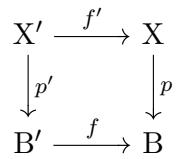
\includegraphics[keepaspectratio]{images/part001_dd3067cf.jpg}}

(E, II, p. 14). 于是我们说“考虑方块图 (1)”，或简单地说“方块 (1)”，以代替说“考虑连续映射的四元组 \(f,f^{\prime},p,p^{\prime}\) ”。称方块 (1) 为交换的，如果等式

\[
f \circ p ^ {\prime} = p \circ f ^ {\prime}
\]

成立。在这情形下，常给 B′、X 与 X′ 分别装备由映射 f、p 与 \(f \circ p' = p \circ f'\) 所定义的 B-空间结构；此时映射 \(p'\) 与 \(f'\) 是 B-态射。

定义 4. --- 我们称方块 (1) 为拓扑空间的笛卡尔方块（或简单地称它是笛卡尔的），如果它是交换的，并且对每个拓扑空间 Y 和每对连续映射 u: Y → B' 与 v: Y → X（满足 f ∘ u = p ∘ v），存在唯一的连续映射 w: Y → X'，满足 p' ∘ w = u 且 f' ∘ w = v。

为使方块 (1) 是笛卡尔的，必须且只需方块

(1')

\pandocbounded{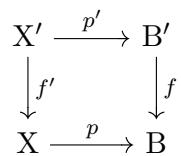
\includegraphics[keepaspectratio]{images/part001_f0fdde30.jpg}}

是笛卡尔的。

命题 1. --- 为使方块 (1) 是笛卡尔的，必须且只需它是交换的，并且对每个 B-空间 Y 和每对 B-态射 \(u\colon Y \to B'\) 、\(v\colon Y \to X\) ，存在唯一的 B-态射 \(w\colon Y \to X'\) ，使得 \(p' \circ w = u\) 且 \(f' \circ w = v\) 。

设方块 (1) 是笛卡尔的。设 Y 为一个 B-空间，\(u: Y \to B'\) 与 \(v: Y \to X\) 为 B-态射。映射 \(f \circ u\) 与 \(p \circ v\) 都等于 B-空间 Y 的投影；于是满足 \(p' \circ w = u\) 与 \(f' \circ w = v\) 的唯一连续映射 w 是一个 B-态射。这就证明了条件的必要性。

反之，设此条件成立。设 Y 为一个拓扑空间，\(u \colon \mathrm{Y} \to \mathrm{B}'\) 与 \(v \colon \mathrm{Y} \to \mathrm{X}\) 为满足 \(f \circ u = p \circ v\) 的连续映射。当 Y 装备上由 \(f \circ u\) 定义的 B-空间结构时，\(u\) 与 \(v\) 是 B-态射。每个连续映射 \(w \colon \mathrm{Y} \to \mathrm{X}'\) ，只要满足 \(p' \circ w = u\) 与 \(f' \circ w = v\) ，就是一个 B-态射，所以这样的映射恰好存在一个。

命题 2. --- 设 B、B' 与 X 为拓扑空间，p: X → B、f: B' → B 为连续映射。

\begin{enumerate}
\def\labelenumi{\alph{enumi})}
\tightlist
\item
  方块
\end{enumerate}

\[
\begin{array}{c} \mathrm{B} ^ {\prime} \times_ {\mathrm{B}} \mathrm{X} \xrightarrow {\mathrm{pr} _ {2}} \mathrm{X} \\ \Biggl \downarrow \mathrm{pr} _ {1} \\ \mathrm{B} ^ {\prime} \xrightarrow {f} \mathrm{B} \end{array}\tag{2}
\]

是一个笛卡尔方块。

\begin{enumerate}
\def\labelenumi{\alph{enumi})}
\setcounter{enumi}{1}
\tightlist
\item
  对每个交换方块
\end{enumerate}

\[
\begin{array}{c} \mathrm {X^ {\prime}} \xrightarrow {f ^ {\prime}} \mathrm{X} \\ \Big \downarrow_ {p ^ {\prime}} \\ \mathrm {B^ {\prime}} \xrightarrow {f} \mathrm{B} \end{array}\tag{3}
\]

存在唯一的连续映射 \(h: X' \to B' \times_{B} X\) ，使得 \(pr_{1} \circ h = p'\) 且 \(pr_{2} \circ h = f'\) 。

\begin{enumerate}
\def\labelenumi{\alph{enumi})}
\setcounter{enumi}{2}
\tightlist
\item
  交换方块 (3) 是笛卡尔的，当且仅当 h 是一个同胚。
\end{enumerate}

断言 \(a\) ) 由命题 1 以及 B-空间的范畴中两个 B-空间的积的泛性质 (I, p. 3) 得出。断言 \(b\) ) 由它得出。

若方块 (3) 是笛卡尔的，则存在唯一的连续映射 \(h'\colon B'\times_{B}X\to X'\) ，使得 \(f'\circ h' = pr_{2}\) 且 \(p'\circ h' = pr_{1}\) 。我们有 \(f'\circ h'\circ h = f'\) 与 \(p'\circ h'\circ h = p'\) ，由于方块 (3) 是笛卡尔的，从而 \(h'\circ h = Id_{X'}\) 。我们有 \(pr_{1}\circ h\circ h' = pr_{1}\) 与 \(pr_{2}\circ h\circ h' = pr_{2}\) ，由于方块 (2) 是笛卡尔的，从而 \(h\circ h' = Id_{B'\times_{B}X}\) 。这就证明了 h 是一个同胚。

反之，设 h 是一个同胚；由于方块 (2) 是笛卡尔的，方块 (3) 也是笛卡尔的。

映射 \(h \colon \mathrm{X}' \to \mathrm{B}' \times_{\mathrm{B}} \mathrm{X}\) ——其存在性与唯一性由前一命题的 \(b)\) 款所断言——将称为典型的：它就是在 I, p. 3 中记作 \((p', f')\) 的映射。

命题 3. --- 设

\[
\begin{array}{c} \mathrm {X^ {\prime}} \xrightarrow {f ^ {\prime}} \mathrm{X} \\ \Big \downarrow_ {p ^ {\prime}} \\ \mathrm {B^ {\prime}} \xrightarrow {f} \mathrm{B} \end{array}
\]

为一个笛卡尔方块。对 \(p'\) 的任一连续截面 s，映射 \(f'\circ s\) 是 f 到 X 中的连续提升。映射 \(s\mapsto f'\circ s\) 是从 \(\mathcal{C}_{\mathrm{B}'}(\mathrm{B}';\mathrm{X}')\) 到 \(\mathcal{C}_{\mathrm{B}}(\mathrm{B}';\mathrm{X})\) 上的一个双射。

若 \(s \colon B' \to X'\) 是 \(p'\) 的一个连续截面，我们有 \(p \circ f' \circ s = f \circ p' \circ s = f\) ，这就证明 \(f' \circ s\) 是 \(f\) 到 X 中的连续提升，即从 \(B'\) 到 X 中的一个 B-态射。反之，设 \(g \colon B' \to X\) 是一个 B-态射。我们有 \(f \circ \mathrm{Id}_{\mathrm{B}'} = p \circ g\) ；于是由笛卡尔方块的定义，存在唯一的连续映射 \(s \colon B' \to X'\) ，使得 \(p' \circ s = \mathrm{Id}_{\mathrm{B}'}\) 且 \(f' \circ s = g\) ，命题得证。

\subsection{由过渡到子空间构造的笛卡尔方块}

命题 4. --- 设

\[
\begin{array}{c} \mathrm {X^ {\prime}} \xrightarrow {f ^ {\prime}} \mathrm{X} \\ \Big \downarrow_ {p ^ {\prime}} \\ \mathrm {B^ {\prime}} \xrightarrow {f} \mathrm{B} \end{array}\tag{4}
\]

为一个笛卡尔方块，并设 \(B_{0}\) 、\(B_{0}^{\prime}\) 、\(X_{0}\) 分别为 B、\(B^{\prime}\) 与 X 的子空间。设 \(f(B_{0}^{\prime}) \subset B_{0}\) ，\(p(X_{0}) \subset B_{0}\) ，并令 \(X_{0}^{\prime} = \overline{p'}^{1}(B_{0}^{\prime}) \cap \overline{f'}^{1}(X_{0})\) 。则方块

\[
\begin{array}{c} \mathrm{X} _ {0} ^ {\prime} \xrightarrow {f _ {0} ^ {\prime}} \mathrm{X} _ {0} \\ \Biggl \downarrow p _ {0} ^ {\prime} \\ \mathrm{B} _ {0} ^ {\prime} \xrightarrow {f _ {0}} \mathrm{B} _ {0} \end{array}\tag{4'}
\]

（其中映射 \(f_0\) 、\(f_0'\) 、\(p_0\) 、\(p_0'\) 分别由 \(f\) 、\(f'\) 、\(p\) 、\(p'\) 过渡到子集得到）是笛卡尔的。

考虑由交换图 (4) 得到的典型映射 \(h \colon X' \to B' \times_B X\) 。由于方块 (4) 是笛卡尔的，\(h\) 是一个同胚。按构造，我们有 \(X_0' = h^{-1}(B_0' \times_{B_0} X_0)\) ，而映射 \(h_0 \colon X_0' \to B_0' \times_{B_0} X_0\) 由交换图 ( \(4'\) ) 得到，它是由 \(h\) 过渡到子集得到的。因此它是一个同胚，从而方块 ( \(4'\) ) 是笛卡尔的 (prop. 2)。

推论. --- 设

\pandocbounded{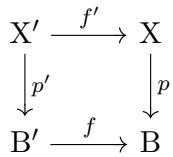
\includegraphics[keepaspectratio]{images/part001_2907af81.jpg}}

为一个笛卡尔方块。

\begin{enumerate}
\def\labelenumi{\alph{enumi})}
\item
  对每个点 \(b'\) （在 \(B'\) 中），映射 \(f'\) 诱导出纤维 \(X_{b'}'\) （\(p'\) 的）到纤维 \(X_{f(b')}\) （\(p\) 的）上的一个同胚。
\item
  若映射 p 是单射（相应地，满射；相应地，双射），则 \(p'\) 亦然。
\end{enumerate}

设 \(b'\) 为 B' 的一点。令 \(b = f(b')\) 。对一切 \(x' \in X_{b'}'\) ，我们有 \(p(f'(x')) = f(p'(x')) = f(b') = b\) ，从而 \(f'(x') \in X_b\) 。这就证明 \(X_{b'}' \subset \overline{f'}^{1}(X_b)\) 。在命题 4 中取 \(B_0 = \{b\}\) 、\(B_0' = \{b'\}\) 与 \(X_0 = X_b\) ；于是有 \(X_0' = X_{b'}'\) ，由此得断言 \(a\) )。

为使映射 p 是单射（相应地，满射；相应地，双射），必须且只需它的每个纤维的基数至多（相应地，至少；相应地，恰好）是 1。断言 b) 由此得出。

例. --- 设 \((X,p)\) 为一个 B-空间，A 为 B 的一个子空间。方块

\[
\begin{array}{c} \overline {{p}} ^ {1} (\mathrm{A}) \xrightarrow {j} \mathrm{X} \\ \Biggl \downarrow p _ {\mathrm{A}} \\ \mathrm{A} \xrightarrow {i} \mathrm{B} \end{array}\tag{5}
\]

（其中 i 与 j 是典型单射）是笛卡尔的。

特别地，若 A 与 A' 是拓扑空间 B 的子空间，则方块

\begin{enumerate}
\def\labelenumi{(\arabic{enumi})}
\setcounter{enumi}{5}
\tightlist
\item
\end{enumerate}

\pandocbounded{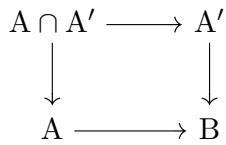
\includegraphics[keepaspectratio]{images/part001_a4278a10.jpg}}

（其中的箭头是典型单射）是笛卡尔的。

\subsection{由积、纤维积与和构造的笛卡尔方块}

命题 5. --- 设 I 为一个集合，且对每个 \(i \in I\) ，设

\[
\begin{array}{c} \mathrm{X} _ {i} ^ {\prime} \xrightarrow {f _ {i} ^ {\prime}} \mathrm{X} _ {i} \\ \Big \downarrow p _ {i} ^ {\prime} \\ \mathrm{B} _ {i} ^ {\prime} \xrightarrow {f _ {i}} \mathrm{B} _ {i} \end{array}\tag{7}
\]

为一个笛卡尔方块。方块

\[
\begin{array}{c} \prod_ {i \in \mathrm{I}} \mathrm{X} _ {i} ^ {\prime} \xrightarrow {f ^ {\prime}} \prod_ {i \in \mathrm{I}} \mathrm{X} _ {i} \\ \Biggl \downarrow^ {p ^ {\prime}} \qquad \qquad \qquad \qquad \Biggl \downarrow^ {p} \\ \prod_ {i \in \mathrm{I}} \mathrm{B} _ {i} ^ {\prime} \xrightarrow {f} \prod_ {i \in \mathrm{I}} \mathrm{B} _ {i} \end{array}\tag{ (7') }
\]

\((\text{其中 } f, f', p, p' \text{ 是这些族 } (f_i), (f'_i), (p_i), (p'_i) \text{ 在乘积上的延拓}) \text{ 是笛卡尔的。}\)

设 Y 为一个拓扑空间，\(u \colon \mathrm{Y} \to \prod_{i} \mathrm{B}_{i}'\) 与 \(v \colon \mathrm{Y} \to \prod_{i} \mathrm{X}_{i}\) 为满足 \(f \circ u = p \circ v\) 的连续映射。对 \(i \in \mathrm{I}\) ，令 \(u_{i} = \mathrm{pr}_{i} \circ u\) 与 \(v_{i} = \mathrm{pr}_{i} \circ v\) ；我们有 \(f_{i} \circ u_{i} = p_{i} \circ v_{i}\) ，且存在唯一的连续映射 \(w_{i} \colon \mathrm{Y} \to \mathrm{X}_{i}'\) ，使得 \(p_{i}' \circ w_{i} = u_{i}\) 且 \(f_{i}' \circ w_{i} = v_{i}\) 。于是映射 \(w = (w_{i})\) 是从 Y 到 \(\prod_{i} \mathrm{X}_{i}'\) 中的一个连续映射，满足 \(p' \circ w = u\) 与 \(f' \circ w = v\) ，并且它是具有这些性质的唯一映射。

推论 1. --- 设 X 为一个 B-空间，p 为其投影，F 为一个拓扑空间。方块

\[
\begin{array}{c} \mathrm{X} \times \mathrm{F} \xrightarrow {\operatorname{pr} _ {1}} \mathrm{X} \\ \Biggl \downarrow p \times \mathrm{Id} _ {\mathrm{F}} \\ \mathrm{B} \times \mathrm{F} \xrightarrow {\operatorname{pr} _ {1}} \mathrm{B} \end{array}\tag{8}
\]

是笛卡尔的。

设 P 为化约为一点的空间。推论 1 由把命题 5 应用于下列笛卡尔方块而得

\[
\begin{array}{l} \mathrm{X} \xrightarrow {\mathrm{Id} _ {\mathrm{X}}} \mathrm{X} \\ \Big \downarrow_ {p} \qquad \Big \downarrow_ {p} \\ \mathrm{B} \xrightarrow {\mathrm{Id} _ {\mathrm{B}}} \mathrm{B} \end{array} \qquad \text {and} \qquad \begin{array}{l} \mathrm{F} \longrightarrow \mathrm{P} \\ \Big \downarrow_ {\mathrm{Id} _ {\mathrm{F}}} \qquad \Big \downarrow_ {\mathrm{Id} _ {\mathrm{P}}} \\ \mathrm{F} \longrightarrow \mathrm{P}. \end{array}
\]

设 B 与 B' 为拓扑空间，\(f: B' \to B\) 为一个连续映射。设 I 为一个集合，且对每个 \(i \in I\) ，设 \(X_i\) 为一个 B-空间，\(X'_i\) 为一个 B'-空间，\(f'_i: X'_i \to X_i\) 为一个连续映射，使得方块

\[
\begin{array}{c} \mathrm{X} _ {i} ^ {\prime} \xrightarrow {f _ {i} ^ {\prime}} \mathrm{X} _ {i} \\ \Big \downarrow \\ \mathrm{B} ^ {\prime} \xrightarrow {f} \mathrm{B} \end{array}\tag{9}
\]

是交换的。存在唯一的连续映射

\[
f ^ {\prime} \colon \prod_ {i \in \mathrm{I}} \mathrm{X} _ {i} ^ {\prime} \to \prod_ {i \in \mathrm{I}} \mathrm{X} _ {i}
\]

满足 \(pr_{i} \circ f' = f_{i}' \circ pr_{i}\) （对一切 \(i \in I\) ），且使得方块

\[
\begin{array}{c} \prod_ {i \in I} X _ {i} ^ {\prime} \xrightarrow {f ^ {\prime}} \prod_ {i \in I} X _ {i} \\ \Big \downarrow \qquad \qquad \qquad \qquad \Big \downarrow \\ B ^ {\prime} \xrightarrow {f} B \end{array}\tag{ (9') }
\]

是交换的（若 I ≠ ∅，这最后一个条件可由其余条件推出）：它是由映射

\[
f \times \prod_ {i \in \mathrm{I}} f _ {i} ^ {\prime} \colon \mathrm{B} ^ {\prime} \times \prod_ {i \in \mathrm{I}} \mathrm{X} _ {i} ^ {\prime} \to \mathrm{B} \times \prod_ {i \in \mathrm{I}} \mathrm{X} _ {i}
\]

过渡到子集而得到的。在这些记号下：

推论 2. --- 若对每个 \(i \in I\) 方块 (9) 都是笛卡尔的，则方块 ( \(9'\) ) 是笛卡尔的。

由命题 5 推出一个笛卡尔方块

\[
\begin{array}{c} \mathrm{B} ^ {\prime} \times \prod_ {i} \mathrm{X} _ {i} ^ {\prime} \xrightarrow {\operatorname{Id} _ {\mathrm{B}} \times \prod_ {i} f _ {i} ^ {\prime}} \mathrm{B} \times \prod_ {i} \mathrm{X} _ {i} \\ \Biggl \downarrow \\ \mathrm{B} ^ {\prime} \times (\mathrm{B} ^ {\prime}) ^ {\mathrm{I}} \xrightarrow {f \times \prod_ {i} f} \mathrm{B} \times \mathrm{B} ^ {\mathrm{I}}  . \end{array}
\]

用 \(\Delta_{\mathrm{B}^{\prime}}\) 与 \(\Delta_{\mathrm{B}}\) 表示 \(\mathrm{B}^{\prime}\times (\mathrm{B}^{\prime})^{\mathrm{I}}\) 与 \(\mathrm{B}\times \mathrm{B}^{\mathrm{I}}\) 的对角线。图表

\[
\begin{array}{c} \prod_ {i \in \mathrm{I}} X _ {i} ^ {\prime} \xrightarrow {f ^ {\prime}} \prod_ {i \in \mathrm{I}} X _ {i} \\ \Big \downarrow \qquad \qquad \qquad \Big \downarrow \\ \Delta_ {\mathrm{B} ^ {\prime}} \xrightarrow {} \Delta_ {\mathrm{B}} \end{array}
\]

由前一个图表过渡到子空间得到，它是笛卡尔的 (I, p. 9, prop. 4)。它等同于图表 (9')。

例 1. --- 设

\[
\begin{array}{c} \mathrm {X^ {\prime}} \xrightarrow {f ^ {\prime}} \mathrm{X} \\ \Big \downarrow_ {p ^ {\prime}} \\ \mathrm {B^ {\prime}} \xrightarrow {f} \mathrm{B} \end{array}
\]

为一个笛卡尔方块。于是推论 2 给出一个笛卡尔方块

\[
\begin{array}{c} \mathrm {X^ {\prime} \times_ {B^ {\prime}} X^ {\prime}} \xrightarrow {\varphi} \mathrm {X\times_ {B} X} \\ \Big \downarrow \\ \mathrm {B^ {\prime} \xrightarrow {f} B}. \end{array}
\]

我们有关系式 \(\overline{\varphi}^{1}(\Delta_{\mathrm{X}}) = \Delta_{\mathrm{X}^{\prime}}\) 。事实上，由 I, p. 8 的命题 2，只需考虑 \(\mathrm{X}' = \mathrm{B}' \times_{\mathrm{B}} \mathrm{X}\) 的情形。设 \(((b,x),(b,x'))\) 为 \(X^{\prime} \times_{B^{\prime}} X^{\prime}\) 的一个元素，其中 \(b \in B^{\prime}\) ，\(x, x^{\prime} \in X\) 。这个元素属于 \(\overline{\varphi}^{1}(\Delta_{\mathrm{X}})\) 当且仅当 \(x = x^{\prime}\) 。

命题 6. --- 设 I 为一个集合，且对每个 \(i \in I\) ，设

\[
\begin{array}{c} \mathrm{X} _ {i} ^ {\prime} \xrightarrow {f _ {i} ^ {\prime}} \mathrm{X} \\ \Biggl \downarrow p _ {i} ^ {\prime} \\ \mathrm{B} _ {i} ^ {\prime} \xrightarrow {f _ {i}} \mathrm{B} \end{array}\tag{10}
\]

为一个笛卡尔方块。设 X' 与 B' 分别为族 \((X'_i)\) 与 \((B'_i)\) 的和空间。设 f: B' → B、f': X' → X 与 p': X' → B' 为分别由族 \((f_i)\) 、\((f'_i)\) 与 \((p'_i)\) 诱导出的映射。方块

\((10')\)

\pandocbounded{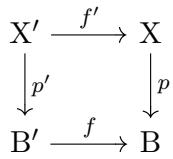
\includegraphics[keepaspectratio]{images/part001_48571453.jpg}}

是笛卡尔的。

映射 \(f\) 、\(f'\) 与 \(p'\) 都是连续的。方块 \((10')\) 的交换性由其定义得出。设 \(h_i\) 表示从 \(\mathrm{X}_i'\) 到 \(\mathrm{B}_i' \times_{\mathrm{B}} \mathrm{X}\) 上的典型同胚 (I, p. 8, 命题 2)，并设 \(h: \mathrm{X}' \to \mathrm{B}' \times_{\mathrm{B}} \mathrm{X}\) 为典型映射 (loc. cit.)。我们有 \(h = h'' \circ h'\) ，其中 \(h': \mathrm{X}' \to \coprod (\mathrm{B}_i' \times_{\mathrm{B}} \mathrm{X})\) 是由诸 \(h_i\) 诱导的同胚，而 \(h'': \coprod (\mathrm{B}_i' \times_{\mathrm{B}} \mathrm{X}) \to (\coprod \mathrm{B}_i') \times_{\mathrm{B}} \mathrm{X}\) 是在 I, p. 4 的例 5 中定义的那个映射。由 I, p. 8 的命题 2 即得结论。

例 2. --- 设 \((X,p)\) 为一个 B-空间，\((\mathrm{A}_{k})_{k\in\mathrm{K}}\) 为 B 的一族子空间。设 A 为族 \((\mathrm{A}_{k})_{k\in\mathrm{K}}\) 的和空间，Y 为族 \((\overline{p}^{1}(\mathrm{A}_{k}))_{k\in\mathrm{K}}\) 的和空间；用 \(i: A \to B\) 、\(j: Y \to X\) 与 \(p': Y \to A\) 分别表示由 \(A_{k}\) 到 B 中的典型单射、\(\overline{p}^{1}(\mathrm{A}_{k})\) 到 X 中的典型单射以及诸映射 \(p_{\mathrm{A}_{k}}: \overline{p}^{1}(\mathrm{A}_{k}) \to \mathrm{A}_{k}\) （\(k \in K\) ）所诱导的映射。方块

\[
\begin{array}{c} \mathrm{Y} \xrightarrow {j} \mathrm{X} \\ \Biggl \downarrow p ^ {\prime} \\ \mathrm{A} \xrightarrow {i} \mathrm{B} \end{array}\tag{11}
\]

是笛卡尔的；这由 I, p. 10 的例与命题 6 得出。

\subsection{笛卡尔方块的复合}

命题 7. --- 设

\[
\begin{array}{c} \mathrm {X^ {\prime\prime}} \xrightarrow {g ^ {\prime}} \mathrm {X^ {\prime}} \\ \Big \downarrow_ {p ^ {\prime \prime}} \\ \mathrm {B^ {\prime\prime}} \xrightarrow {g} \mathrm {B^ {\prime}} \end{array}\tag{12}
\]

和

\begin{enumerate}
\def\labelenumi{(\arabic{enumi})}
\setcounter{enumi}{12}
\tightlist
\item
\end{enumerate}

\pandocbounded{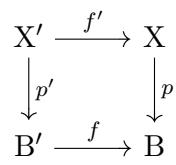
\includegraphics[keepaspectratio]{images/part001_4552bd62.jpg}}

为两个交换方块；考虑方块

\begin{enumerate}
\def\labelenumi{(\arabic{enumi})}
\setcounter{enumi}{13}
\tightlist
\item
\end{enumerate}

\pandocbounded{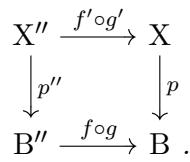
\includegraphics[keepaspectratio]{images/part001_1603e4c4.jpg}}

它是交换的。若方块 (12) 与 (13) 都是笛卡尔的，则方块 (14) 亦然。若方块 (13) 与 (14) 都是笛卡尔的，则方块 (12) 亦然。

方块 (14) 是交换的，因为我们有 \(p \circ f' \circ g' = f \circ p' \circ g' = f \circ g \circ p''\) 。用 \(h' : X'' \to B'' \times_{B'} X'\) 、\(h : X' \to B' \times_{B} X\) 与 \(h'' : X'' \to B'' \times_{B} X\) 表示分别由交换方块 (12)、(13) 与 (14) 得到的典型连续映射。此外，用

\[
j \colon \mathrm{B} ^ {\prime \prime} \times_ {\mathrm{B}} \mathrm{X} \rightarrow \mathrm{B} ^ {\prime \prime} \times_ {\mathrm{B} ^ {\prime}} (\mathrm{B} ^ {\prime} \times_ {\mathrm{B}} \mathrm{X})
\]

表示把 \((b'', x)\) 映为 \((b'', g(b''), x)\) 的连续映射。它是一个同胚，并且有 \(j \circ h'' = (\mathrm{Id}_{\mathrm{B}''} \times_{\mathrm{B}} h) \circ h'\) 。

设方块 (13) 是笛卡尔的。于是 h 是一个同胚 (I, p. 8, prop 2)，从而映射 \(Id_{B''} \times_{B} h\) 是一个同胚，并且 \(h''\) 是同胚当且仅当 \(h'\) 是同胚。这就是说，方块 (12) 是笛卡尔的当且仅当方块 (14) 是笛卡尔的 (loc. cit.)。

采用命题 7 中的记号，有时称方块 (14) 为方块 (13) 与 (12) 的复合方块。第一个断言表明：两个笛卡尔方块的复合是笛卡尔的。特别地，B''-空间 \(g^{*}(f^{*}(\mathrm{X}))\) 与 \((f \circ g)^{*}(\mathrm{X})\) 是同构的。

\pandocbounded{
\includegraphics[keepaspectratio]{images/part001_52f28a70.jpg}}

注. --- 1) 可能发生这样的情形：方块 (12) 与 (14) 都是笛卡尔的，而方块 (13) 却不是 (I, p. 139, exerc. 2)。

\begin{enumerate}
\def\labelenumi{\arabic{enumi})}
\setcounter{enumi}{1}
\tightlist
\item
  设 \(p \colon \mathrm{X} \to \mathrm{B}\) 与 \(f \colon \mathrm{B}' \to \mathrm{B}\) 为连续映射。映射 \(g \colon \mathrm{B}' \to \mathrm{B}' \times \mathrm{B}\) （由 \(g(b') = (b', f(b'))\) 定义）是从 \(\mathrm{B}'\) 到图像 \(\mathrm{G}\) （映射 \(f\) 的）上的一个同胚 (TG, I, p. 25, cor. 2)，而纤维积 \(\mathrm{B}' \times_{\mathrm{B}} \mathrm{X}\) 可以等同 (I, p. 6) 于 \(\mathrm{B}' \times \mathrm{X}\) 的一个子空间，即 \(\mathrm{G}\) 在映射 \(\mathrm{Id}_{\mathrm{B}'} \times p \colon \mathrm{B}' \times \mathrm{X} \to \mathrm{B}' \times \mathrm{B}\) 下的原像。由 I, p. 10 的例与命题 5 的推论 1 (I, p. 11)，方块
\end{enumerate}

\[
\begin{array}{c c} \mathrm {B^ {\prime}} \times_ {\mathrm{B}} \mathrm{X} \xrightarrow {i} \mathrm {B^ {\prime}} \times \mathrm{X} & \mathrm {B^ {\prime}} \times \mathrm{X} \xrightarrow {\mathrm{pr} _ {2}} \mathrm{X} \\ \Biggl \downarrow \mathrm{pr} _ {1} & \Biggl \downarrow \mathrm{Id} _ {\mathrm {B^ {\prime}}} \times p \\ \mathrm {B^ {\prime}} \xrightarrow {g} \mathrm {B^ {\prime}} \times \mathrm{B} & \text {et} \end{array} \qquad \qquad \begin{array}{c c} \mathrm {B ^ {\prime}} \times \mathrm{X} \xrightarrow {\mathrm{pr} _ {2}} \mathrm{X} \\ \Biggl \downarrow \mathrm{Id} _ {\mathrm {B^ {\prime}}} \times p & \Biggl \downarrow p \\ \mathrm {B^ {\prime}} \times \mathrm{B} \xrightarrow {\mathrm{pr} _ {2}} \mathrm{B} & \end{array}
\]

（其中 i 表示典型单射）都是笛卡尔的，而笛卡尔方块

\[
\begin{array}{c} \mathrm{B} ^ {\prime} \times_ {\mathrm{B}} \mathrm{X} \xrightarrow {\mathrm{pr} _ {2}} \mathrm{X} \\ \Big \downarrow \mathrm{pr} _ {1} \\ \mathrm{B} ^ {\prime} \xrightarrow {f} \mathrm{B} \end{array}
\]

是它们的复合。换句话说，每个笛卡尔方块都等同于一个由取积得到的笛卡尔方块 (I, p. 11, 命题 5 的推论 1, 方块 (8)) 与一个由过渡到子空间得到的笛卡尔方块 (I, p. 10, 例, 方块 (5)) 的复合方块。

\begin{enumerate}
\def\labelenumi{\arabic{enumi})}
\setcounter{enumi}{2}
\tightlist
\item
  设
\end{enumerate}

\[
\begin{array}{c} \mathrm{X} _ {1} \xrightarrow {g _ {1}} \mathrm{X} \\ \Biggl \downarrow p _ {1} \\ \mathrm{B} _ {1} \xrightarrow {f _ {1}} \mathrm{B} \end{array}\tag{15}
\]

和

\[
\begin{array}{c} \mathrm{X} _ {2} \xrightarrow {g _ {2}} \mathrm{X} \\ \Biggl \downarrow p _ {2} \\ \mathrm{B} _ {2} \xrightarrow {f _ {2}} \mathrm{B} \end{array}\tag{16}
\]

  设

\[
\begin{array}{c} \mathrm{X} _ {1} \times_ {\mathrm{X}} \mathrm{X} _ {2} \xrightarrow {g} \mathrm{X} \\ \Big \downarrow^ {p ^ {\prime}} \\ \mathrm{B} _ {1} \times_ {\mathrm{B}} \mathrm{B} _ {2} \xrightarrow {f} \mathrm{B} \end{array}\tag{17}
\]

其中 \(f\) （相应地，\(g\) ）是在纤维积 \(\mathrm{B}_{1} \times_{\mathrm{B}} \mathrm{B}_{2}\) （相应地，纤维积 \(\mathrm{X}_{1} \times_{\mathrm{X}} \mathrm{X}_{2}\) ）上定义 B-空间（相应地，X-空间）结构的映射，而 \(p'\) 是由 \(p_{1} \times p_{2}\) 过渡到子空间所诱导的映射。它是笛卡尔的 (I, p. 13, 命题 5 的推论 2)。

现在考虑下面两个交换方块：

\[
\begin{array}{c c} \mathrm{X} _ {1} \times_ {\mathrm{X}} \mathrm{X} _ {2} \xrightarrow {\operatorname{pr} _ {1}} \mathrm{X} _ {1} & \mathrm{X} _ {1} \times_ {\mathrm{X}} \mathrm{X} _ {2} \xrightarrow {\operatorname{pr} _ {2}} \mathrm{X} _ {2} \\ \Biggl \downarrow p ^ {\prime} & \text {and} \\ \mathrm{B} _ {1} \times_ {\mathrm{B}} \mathrm{B} _ {2} \xrightarrow {\operatorname{pr} _ {1}} \mathrm{B} _ {1} & \mathrm{(19)} \\ & \mathrm{B} _ {1} \times_ {\mathrm{B}} \mathrm{B} _ {2} \xrightarrow {\operatorname{pr} _ {2}} \mathrm{B} _ {2}. \end{array}\tag{18}
\]

方块 (17) 由方块 (15) 与 (18) 复合而成，也由方块 (16) 与 (19) 复合而成。由命题 7，方块 (18) 与 (19) 都是笛卡尔的。

\subsection{严格映射}

命题 8. --- 设

\[
\begin{array}{c} \mathrm {X^ {\prime}} \xrightarrow {f ^ {\prime}} \mathrm{X} \\ \Big \downarrow_ {p ^ {\prime}} \\ \mathrm {B^ {\prime}} \xrightarrow {f} \mathrm{B} \end{array}
\]

为一个笛卡尔方块。若映射 p 是开的（相应地，是逆紧的；相应地，在每点的一个邻域内有连续截面），则 \(p'\) 亦然。

由 I, p. 16 的注 2，只需对下列类型的笛卡尔方块证明该命题：

\[
\begin{array}{c c} \overline {{p}} ^ {1} (\mathrm {A}) \xrightarrow {j} \mathrm{X} & \mathrm {A} \times \mathrm{F} \xrightarrow {i} \mathrm{X} \times \mathrm{F} \\ \Big \downarrow_ {p _ {\mathrm {A}}} & \Big \downarrow_ {p \times \mathrm {Id}_{\mathrm {F}}} \\ \mathrm {A} & \xrightarrow {i} \mathrm {B} \end{array} \quad\text {and} \quad \begin{array}{c} \mathrm {X} \times \mathrm {F} \xrightarrow {j} \mathrm {X} \\ \Big \downarrow_ {p \times \mathrm {Id}_{\mathrm {F}}} \\ \mathrm {B} \times \mathrm {F} \xrightarrow {i} \mathrm {B} \end{array}
\]

其中 F 是一个拓扑空间，A 是 B 的一个子空间，i 与 j 是典型单射。若映射 p 是开的，则映射 \(p_{A}\) 与 \(p \times Id_{F}\) 是开的 (TG, I, p. 30, prop. 2 与 TG, I, p. 34, prop. 8)。若映射 p 是逆紧的，则映射 \(p_{A}\) 与 \(p \times Id_{F}\) 是逆紧的 (TG, I, p. 72, prop. 3 与 TG, I, p. 72, def. 1)。若 U 是 B 的一个开子集，且 \(s\colon\mathrm{U}\to\mathrm{X}\) 是 p 在 U 上的一个连续截面，则映射 \(s\mid(\mathrm{A}\cap\mathrm{U})\) 是 \(p_{\mathrm{A}}\) 在 \(\mathrm{A}\cap\mathrm{U}\) 上的一个连续截面，而映射 \(s\times\mathrm{Id}_{\mathrm{F}}\) 是 \(p\times\mathrm{Id}_{\mathrm{F}}\) 在 \(\mathrm{U}\times\mathrm{F}\) 上的一个连续截面。

注 1. --- 采用命题 8 中的记号，若 \(p\) 是闭映射，则 \(p'\) 未必是闭的 (cf. TG, I, p. 32, prop. 3)。然而，若 \(p\) 是有连续截面的映射，则 \(p'\) 也有连续截面。

定义 5. --- 设 X 与 Y 为拓扑空间，f: X → Y 为一个映射。设 R 为与 f 相伴的等价关系，且

\[
\mathrm{X} \rightarrow \mathrm{X} / \mathrm{R} \xrightarrow {g} f (\mathrm{X}) \rightarrow \mathrm{Y}
\]

为 \(f\) 的典型分解 (E, II, p. 44)。我们称映射 \(f\) 是严格的，如果 \(g\) （当 \(X/R\) 装备商拓扑而 \(f(X)\) 装备由 \(Y\) 的拓扑诱导的拓扑时）是一个同胚。

严格映射是连续的。

回顾 (TG, I, p. 22, prop. 8)：为使映射 \(f\) 是严格的，必须且只需 \(f\) 是连续的，并且对每个子集 \(A\) （在 \(X\) 中是开的（相应地，闭的）且饱和的），\(f(A)\) 在 \(f(X)\) 中是开的（相应地，闭的）。

例. --- 1) 两个严格映射的复合未必是严格的。事实上，每个连续映射 \(f \colon X \to Y\) 都是映射 \(\mathrm{pr}_2 \colon X \times Y \to Y\) 与映射 \(x \mapsto (x, f(x))\) （从 \(X\) 到 \(X \times Y\) 中）的复合，而这两个映射都是严格的 (TG, I, p. 26, prop. 5 与 TG, I, p. 25, cor. 2)。另一方面，两个严格且单射（相应地，满射）的映射的复合是一个严格映射。

\begin{enumerate}
\def\labelenumi{\arabic{enumi})}
\setcounter{enumi}{1}
\item
  一个开的、闭的或有连续截面的连续映射是严格的。这由 TG, I, p. 32 的命题 3 与 TG, I, p. 22 的命题 9 得出。
\item
为使从一个拓扑群到另一个拓扑群的连续同态是一个严格态射 (TG, III, p. 16, def. 1)，必须且只需它是定义 5 意义下的严格映射。
\end{enumerate}

命题 9. --- 设 X、Y 与 Z 为拓扑空间。设 \(f\colon X \to Y\) 为一个连续满射映射，\(g\colon Y \to Z\) 为一个映射。

\begin{enumerate}
\def\labelenumi{\alph{enumi})}
\item
若 f 是严格的且 g∘f 是连续的，则映射 g 是连续的。
\item
若 g 是连续的且 g∘f 是严格的，则 g 是严格的。
\item
若 f 与 g \(\circ\) f 都是严格的，则 g 是严格的。
\end{enumerate}

我们来证明断言 a)。用 R 表示 X 中与 f 相伴的关系；按假设，由 f 过渡到商所诱导的从 X/R 到 Y 上的映射是一个同胚。于是第一个断言由 I, p. 21 的命题 6 得出。

我们来证明 b)。设 B 为 Y 的一个闭子集，它对由 g 定义的关系是饱和的，并令 \(A = f^{-1}(B)\) 。由于 f 是连续的，A 在 X 中是闭的，且 A 对由 \(g \circ f\) 定义的等价关系是饱和的。由于 \(g \circ f\) 是严格的且 f 是满射，\(g(B) = g \circ f(A)\) 在 Z 中是闭的。于是连续映射 g 是严格的。

断言 c) 由断言 a) 与 b) 立即得出。

命题 10. --- 设 X 为一个拓扑空间，R 为 X 上的一个等价关系。设 Y 为一个局部紧拓扑空间。设 S 为 X × Y 上的等价关系，它是 X 上的等价关系 R 与 Y 上的相等关系之积。典型双射 (X × Y)/S → (X/R) × Y 是一个同胚。

回顾：若 U 与 V 为拓扑空间，则 \(\mathcal{C}_{c}(\mathrm{U};\mathrm{V})\) 表示从 U 到 V 中的连续映射所成的集合，装备紧开拓扑 (TG, X, p. 26, def. 1)。

设 \(p \colon \mathrm{X} \to \mathrm{X} / \mathrm{R}\) 与 \(q \colon \mathrm{X} \times \mathrm{Y} \to (\mathrm{X} \times \mathrm{Y}) / \mathrm{S}\) 为典型满射。设 \(g \colon (\mathrm{X} \times \mathrm{Y}) / \mathrm{S} \to (\mathrm{X} / \mathrm{R}) \times \mathrm{Y}\) 为典型双射。它是连续的；用 \(h\) 表示它的逆映射，并证明它是连续的。

映射 \(i\colon X \to \mathcal{C}_{c}(Y;X \times Y)\) ——对每个 \(x \in X\) ，\(i(x)\) 是由 \(y \mapsto (x,y)\) 定义的映射——是连续的 (TG, X, p. 28, 定理 3)。映射 \(\widetilde{q}\colon \mathcal{C}_{c}(Y;X \times Y) \to \mathcal{C}_{c}(Y;(X \times Y)/S)\) 把连续映射 \(\varphi\) 对应为映射 \(q \circ \varphi\) ，它是连续的 (TG, X, p. 29, 命题 9)。因此，映射 \(\widetilde{q} \circ i\colon X \to \mathcal{C}_{c}(Y;(X \times Y)/S)\) 是连续的。它与等价关系 R 相容；于是唯一的映射 \(j\colon X/R \to \mathcal{C}_{c}(Y;(X \times Y)/S)\) ——它满足 \(j \circ p = \widetilde{q} \circ i\) ——是连续的。我们有 \(h(\xi,y) = j(\xi)(y)\) ，对每个对 \((\xi,y) \in (X/R) \times Y\) 。由于 Y 是局部紧的，由 TG, X, p. 28 的定理 3，\(h\) 是连续的。

若 Y 不是局部紧的，命题 10 的结论未必成立 (TG, I, p. 96, exerc. 6)。

推论. --- 设 X 与 Y 为拓扑空间，\(f: X \to Y\) 为一个连续映射。设 T 为一个局部紧拓扑空间。若映射 f 是严格的，则映射 \(f \times Id_{T}\) （从 \(X \times T\) 到 \(Y \times T\) 中）亦然。

\subsection{普遍严格映射}

设

\[
\begin{array}{c} \mathrm {X^ {\prime}} \xrightarrow {f ^ {\prime}} \mathrm{X} \\ \Big \downarrow_ {p ^ {\prime}} \\ \mathrm {B^ {\prime}} \xrightarrow {f} \mathrm{B} \end{array}
\]

为一个笛卡尔方块，其中 p 是严格的。映射 \(p'\) 未必是严格的 (cf. 注 1)。然而，若 A 在 B 中是开的（相应地，闭的），则映射 \(p_A: \overline{p}^{1}(A) \to A\) 是严格的。

定义 6. --- 设 p: X → B 为一个映射。我们称 p 是普遍严格的，如果对每个笛卡尔方块

\pandocbounded{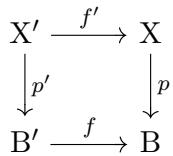
\includegraphics[keepaspectratio]{images/part001_50963eb1.jpg}}

映射 p' 是严格的。

普遍严格映射是严格的。采用定义 6 中的记号，若 \(p\) 是普遍严格的，则 \(p'\) 也是普遍严格的。这由定义立即得出。

推论. --- 开映射、逆紧映射以及具有连续局部截面的映射都是普遍严格的。

例. --- 设 B 为一个拓扑空间，\((\mathrm{A}_{i})_{i\in\mathrm{I}}\) 为 B 的一个覆盖；用 A 表示族 \((\mathrm{A}_{i})_{i\in\mathrm{I}}\) 的和空间，用 \(p: A \to B\) 表示典型映射。在下列两个假设中的每一个之下，映射 p 都是普遍严格的：

\begin{enumerate}
\def\labelenumi{(\roman{enumi})}
\item
  对每个点 \(b \in B\) ，存在 \(i \in I\) ，使得 b 是 \(A_{i}\) 的一个内点；
\item
  族 \((A_{i})\) 是局部有限的，且诸 \(A_{i}\) 是 B 的闭子集。
\end{enumerate}

在假设 (i) 之下，映射 p 在每点的一个邻域内有连续截面。在假设 (ii) 之下，映射 p 按和空间的定义（相应地，由 TG, I, p. 6, prop. 4 与 TG, I, p. 75, th. 1）是逆紧的。因此它是普遍严格的。

注. --- 闭映射未必是普遍严格的 (cf. TG, I, p. 96, exerc. 6)。

命题 11. --- 设

\pandocbounded{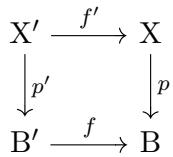
\includegraphics[keepaspectratio]{images/part001_02f1b349.jpg}}

为一个笛卡尔方块。

\begin{enumerate}
\def\labelenumi{\alph{enumi})}
\item
设 f 是严格且满射的。于是，若 p' 是开的（相应地，闭的；相应地，逆紧的），则 p 亦然。
\item
设 f 是闭且满射的。若 p' 是严格的，则 p 是严格的。
\item
设 f 是普遍严格的。若 p' 是普遍严格的，则 p 是普遍严格的。
\end{enumerate}

首先注意，对 X 的每个子集 A，我们有

\[
p ^ {\prime} ((\stackrel {- 1} {f ^ {\prime}}) (\mathrm{A})) = \stackrel {- 1} {f} (p (\mathrm{A})).\tag{20}
\]

事实上，若 \(x' \in (f')^{-1}(\mathrm{A})\) ，则 \(f(p'(x')) = p \circ f'(x') \in p(\mathrm{A})\) 。反之，若 \(b' \in f^{-1}(p(\mathrm{A}))\) ，设 \(x \in A\) 满足 \(f(b') = p(x)\) 。由笛卡尔方块的定义，存在唯一的 \(x' \in X'\) ，使得 \(f'(x') = x\) 且 \(p'(x') = b'\) ，从而 \(b' \in p'((f')^{-1}(\mathrm{A}))\) 。

设 f 是一个开映射且 \(p'\) 是一个严格映射。

集合 \((f')^{-1}(\mathrm{A})\) 在 \(\mathrm{X}'\) 中是开的（相应地，闭的）。于是集合 \(p'((f')^{-1}(\mathrm{A}))\) 在 \(\mathrm{B}'\) 中是开的（相应地，闭的）。由关系式 (20)，它对由 \(f\) 定义的等价关系也是饱和的。由于映射 \(f\) 假设为满射，我们有 \(p(\mathrm{A}) = f(p'((f')^{-1}(\mathrm{A})))\) ，又由于它是严格的，集合 \(p(\mathrm{A})\) 在 B 中是开的（相应地，闭的）。于是映射 \(p\) 是开的（相应地，闭的）。

为使一个连续映射是逆紧的，必须且只需它是闭的且它的纤维是拟紧的 (TG, I, p. 75, th. 1)。若映射 \(p'\) 是逆紧的，则由前所证，映射 \(p\) 是闭的。我们来研究它的纤维：若 \(b \in B\) ，设 \(b' \in B'\) 满足 \(f(b') = b\) 。由 I, p. 10 的推论，映射 \(f'\) 诱导出一个同胚 \(X_{b'}' \to X_b\) 。由于 \(p'\) 是逆紧的，\(X_{b'}'\) 是拟紧的，从而 \(X_b\) 也是。于是映射 \(p\) 是逆紧的。

我们来证明 b) 与 c)。令 \(Y = p(X)\) ，\(Y' = p'(X')\) 。把关系式 (20) 应用于 X，就得到 \(Y' = f^{-1}(Y)\) 。用 g 表示由 f 诱导的从 \(Y'\) 到 Y 中的映射。在情形 b)，由 I, p. 18 的注 1，映射 g 是严格的。在情形 c)，由定义 6 它是严格的，因为方块

\pandocbounded{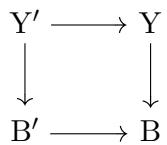
\includegraphics[keepaspectratio]{images/part001_f35053b2.jpg}}

是笛卡尔的。

用 \(q\) 与 \(q'\) 分别表示从 X 到 Y 以及从 \(X'\) 到 \(Y'\) 中的映射，它们由映射 \(p\) 与 \(p'\) 诱导。

\[
\begin{array}{c} \mathrm {X^ {\prime}} \xrightarrow {f ^ {\prime}} \mathrm{X} \\ \Big \downarrow q ^ {\prime} \\ \mathrm {Y^ {\prime}} \xrightarrow {g} \mathrm{Y} \end{array}
\]

由于 \(f\) 是满射，\(f'\) 也是满射；由命题 9 b)，\(p\) 是严格的。

推论 1. --- 设映射 f 是普遍严格且满射的，且映射 p' 是普遍严格的。则映射 p 是普遍严格的。

设

\[
\begin{array}{c} \mathrm{Y} \xrightarrow {g ^ {\prime}} \mathrm{X} \\ \Biggl \downarrow q \\ \mathrm{C} \xrightarrow {g} \mathrm{B} \end{array}
\]

为一个笛卡尔方块；目标是证明映射 q 是严格的。由 I, p. 16 的注 3，方块

\[
\begin{array}{c} \mathrm {X^ {\prime}} \times_ {\mathrm{X}} \mathrm{Y} \xrightarrow {\mathrm{pr} _ {1}} \mathrm {X^ {\prime}} \\ \Biggl \downarrow r \\ \mathrm {B^ {\prime}} \times_ {\mathrm{B}} \mathrm{C} \xrightarrow {\mathrm{pr} _ {1}} \mathrm {B^ {\prime}} \end{array}
\]

和

\[
\begin{array}{c} \mathrm {X^ {\prime} \times_ {X} Y\xrightarrow {pr_ {2}} Y} \\ \Big \downarrow r \\ \mathrm {B^ {\prime} \times_ {B} C\xrightarrow {pr_ {2}} C} \end{array}\tag{21}
\]

都是笛卡尔的，其中 \(r \colon X' \times_{X} Y \to B' \times_{B} C\) 表示由 \((p', q)\) 诱导的映射。由于映射 \(f\) 是普遍严格且满射的，映射 \(\mathrm{pr}_2 \colon B' \times_{B} C \to C\) 亦然 (I, p. 20, def. 6 与 I, p. 10, prop. 4 的推论)。另一方面，映射 \(r\) 是严格的，因为 \(p'\) 假设为普遍严格的。把命题 11 c) 应用于笛卡尔方块 (21)，映射 \(q\) 是严格的。

推论 2. --- 设 B 与 X 为拓扑空间，\(p\colon X \to B\) 为一个连续映射。设 \((A_i)_{i \in I}\) 为 B 的一族子集，它构成 B 的一个开覆盖，或者构成 B 的一个局部有限的闭覆盖。若对每个 \(i \in I\) ，映射 \(p_{A_i}\colon \overline{p}^1(A_i) \to A_i\) 都是严格的（相应地，普遍严格的），则映射 p 是严格的（相应地，普遍严格的）。

对每个 \(i \in \mathrm{I}\) ，令 \(\mathrm{Y}_i = \overline{p}^{1}(\mathrm{A}_i)\) ，\(p_i = p_{\mathrm{A}_i}\) 。设 A 为族 \((\mathrm{A}_i)_{i \in \mathrm{I}}\) 的和空间，Y 为族 \((\mathrm{Y}_i)_{i \in \mathrm{I}}\) 的和空间；用 \(f: \mathrm{A} \to \mathrm{B}\) （相应地，\(g: \mathrm{Y} \to \mathrm{X}\) ，\(q: \mathrm{Y} \to \mathrm{A}\) ）表示由典型单射的族 \(A_i \rightarrow B\) （相应地，典型单射的族 \(Y_i \rightarrow X\) 与诸映射 \(p_i\) ）诱导的映射。方块

\[
\begin{array}{c} \mathrm{Y} \xrightarrow {g} \mathrm{X} \\ \Big \downarrow q \\ \mathrm{A} \xrightarrow {f} \mathrm{B} \end{array}
\]

是一个笛卡尔方块 (例, I, p. 10 与 p. 14)。由 I, p. 20 的推论，映射 \(f\) 是普遍严格的。于是由命题 11，只需证明映射 \(q\) 是严格的（相应地，普遍严格的），如果诸映射 \(p_i\) （\(i \in I\) ）是严格的（相应地，普遍严格的）。这样我们就把该推论的证明化归为这样的情形：诸集合 \(A_i\) （\(i \in I\) ）构成空间 B 的一个由既开又闭的部分组成的分拆，以下即作此假设。

设诸映射 \(p_i\) （\(i \in I\) ）中的每一个都是严格的。若 U 是 X 的一个开子集，且对由 p 定义的等价关系是饱和的，则集合 \(p_i(\mathrm{X}_i \cap \mathrm{U})\) 在 \(\mathrm{A}_i\) 中是开的，从而 \(p(\mathrm{U}) = \bigcup_{i \in \mathrm{I}} p_i(\mathrm{X}_i \cap \mathrm{U})\) 在 B 中是开的。于是映射 p 是严格的。

现在设诸映射 \(p_{i}, i \in I\) 中的每一个都是普遍严格的，我们来证明映射 p 是普遍严格的。设 C 为一个拓扑空间，\(h: C \to B\) 为一个连续映射。目标是证明映射 \(pr_{1}: X \times_{B} C \to C\) 是严格的。空间 C 等同于族 \(C_{i} = h^{-1}(A_{i})\) 的和空间，而空间 \(X \times_{B} C\) 等同于族 \(X \times_{B} C_{i} = X_{i} \times_{A_{i}} C_{i}\) 的直和空间。由于 \(p_{i}\) 是普遍严格的，映射 \(pr_{1}: X_{i} \times_{A_{i}} C_{i} \to C_{i}\) 是严格的。由前所证，映射 \(pr_{1}: X \times_{B} C \to C\) 是严格的。这就证明了映射 p 是普遍严格的。

\section{平展映射}

\subsection{分离映射}

命题 1. --- 设 X 与 Y 为拓扑空间，\(f\colon X \to Y\) 为一个连续映射。下列性质是等价的：

\begin{enumerate}
\def\labelenumi{(\roman{enumi})}
\item
  对角线 \(\Delta_{X}\) （纤维积 X \(\times_{Y}\) X 的）是一个闭子空间；
\item
  对每个拓扑空间 W 与每对从 W 到 X 中的连续映射 \((g_{1}, g_{2})\) （满足 \(f \circ g_{1} = f \circ g_{2}\) ），点 \(w \in W\) （满足 \(g_{1}(w) = g_{2}(w)\) ）所成的集合在 W 中是闭的；
\item
  对每对点 \((x_{1}, x_{2})\) （X 中的），满足 \(x_{1} \neq x_{2}\) 且 \(f(x_{1}) = f(x_{2})\) ，存在一个邻域 \(V_{1}\) （\(x_{1}\) 的，在 X 中）与一个邻域 \(V_{2}\) （\(x_{2}\) 的，在 X 中），使得 \(V_{1} \cap V_{2} = \varnothing\) ；
\end{enumerate}

(i)⇒(ii)：设 \(g_{1}\) 与 \(g_{2}\) 为从 W 到 X 中的连续映射，满足 \(f \circ g_{1} = f \circ g_{2}\) ，并设 \(g: W \to X \times_{Y} X\) 为由 \(g_{1}\) 与 \(g_{2}\) 诱导的映射。由点 \(w \in W\) （满足 \(g_{1}(w) = g_{2}(w)\) ）组成的集合就是 \(g^{-1}(\Delta_{X})\) 。由于 g 是连续的，若对角线 \(\Delta_{X}\) 是闭的，则它是闭的。

(ii)⇒(i)：对角线 \(\Delta_{X}\) 是由点 \(z \in X \times_{Y} X\) （满足 \(\mathrm{pr}_{1}(z) = \mathrm{pr}_{2}(z)\) ）组成的集合。把 (ii) 应用于 \(W = X \times_{Y} X\) 与映射对 \((\mathrm{pr}_{1}, \mathrm{pr}_{2})\) ，即得对角线 \(\Delta_{X}\) 在 \(X \times_{Y} X\) 中是闭的。

(i)⇔(iii)：设 \((x_{1}, x_{2})\) 为 \(X \times_{Y} X\) 的一个点，并设 \(V_{1}\) 与 \(V_{2}\) 分别为 \(x_{1}\) 与 \(x_{2}\) 的邻域。条件 \(V_{1} \cap V_{2} = \varnothing\) 等价于条件 \((\mathrm{V}_{1} \times \mathrm{V}_{2}) \cap \Delta_{\mathrm{X}} = \varnothing\) ，也就是等价于 \((\mathrm{V}_{1} \times \mathrm{V}_{2}) \cap (\mathrm{X} \times_{\mathrm{Y}} \mathrm{X}) \cap \Delta_{\mathrm{X}} = \varnothing\) 。由于诸集合 \((\mathrm{V}_{1} \times \mathrm{V}_{2}) \cap (\mathrm{X} \times_{\mathrm{Y}} \mathrm{X})\) 构成 \((x_{1}, x_{2})\) 在 \(X \times_{Y} X\) 中的一个邻域基，这就证明了 (i) 与 (iii) 的等价性。

定义 1. --- 设 X 与 Y 为拓扑空间。连续映射 \(f: X \to Y\) 称为分离的，如果它满足命题 1 的诸等价条件。

命题 2. --- 设 X、Y、Z 为拓扑空间，\(f\colon X \to Y\) 与 \(g\colon Y \to Z\) 为连续映射。

\begin{enumerate}
\def\labelenumi{\alph{enumi})}
\item
  若 f 与 g 都是分离的，则 \(g \circ f\) 是分离的。
\item
若 g \(\circ\) f 是分离的，则 f 是分离的。
\item
  再设映射 f 是逆紧且满射的。于是，若 g ∘ f 是分离的，则 g 是分离的。
\end{enumerate}

在 X×X 中考虑子空间 \(\Delta_{X}\) （对角线）、\(X \times_Y X\) 与 \(X \times_Z X\) 。它们分别是 X×X 中满足 \(\mathrm{pr}_{1}(u)=\mathrm{pr}_{2}(u)\) 、\(f\circ\mathrm{pr}_{1}(u)=f\circ\mathrm{pr}_{2}(u)\) 、\(g\circ f\circ\mathrm{pr}_{1}(u)=g\circ f\circ\mathrm{pr}_{2}(u)\) 的点 u 所成的集合。若 \(g\circ f\) 是分离的，则 \(\Delta_{X}\) 在 \(X \times_Z X\) 中是闭的，从而在 \(X \times_Y X\) 中也是闭的，由此得 b)。

把命题 1 (ii) 应用于 W = X ×\_Z X、\(g_1 = f \circ \text{pr}_1\) 与 \(g_2 = f \circ \text{pr}_2\) ，则 X ×\_Y X 在 X ×\_Z X 中是闭的，只要 \(g\) 是分离的。此外，若 \(f\) 是分离的，则 \(\Delta_X\) 在 X ×\_Y X 中是闭的 (命题 1, (i))，从而在 X ×\_Z X 中也是闭的，由此得 \(a\) 。

最后，我们来证明 \(c\) 。映射 \((f, f) \colon X \times X \to Y \times Y\) 是逆紧的 (TG, I, p. 73, prop. 4)。子空间 \(X \times_Z X\) 是 \(Y \times_Z Y\) 在 \((f, f)\) 下的原像；由 TG, I, p. 72, prop. 3，映射 \(u \colon X \times_Z X \to Y \times_Z Y\) （由 \((f, f)\) 诱导）是逆紧的。由于 \(g \circ f\) 是分离的，对角线 \(\Delta_X\) 在 \(X \times_Z X\) 中是闭的。于是 \(u(\Delta_X)\) 在 \(Y \times_Z Y\) 中是闭的。由于 \(f\) 是满射，\(u(\Delta_X)\) 是 \(Y \times_Z Y\) 的对角线。这就表明 \(g\) 是分离的。

注. --- 1) 单射的连续映射是分离的。

\begin{enumerate}
\def\labelenumi{\arabic{enumi})}
\setcounter{enumi}{1}
\tightlist
\item
  为使一个拓扑空间 X 是豪斯多夫的 (TG, I, p. 52, def. 1)，必须且只需从 X 到一个化为一点的空间的映射是分离的。在这情形下，从 X 到一个拓扑空间中的每个连续映射都是分离的 (命题 1, (iii))。
\end{enumerate}

设 \(f\colon X \to Y\) 为一个连续且分离的映射。对每个点 \(y\) （\(Y\) 中的），纤维 \(f^{-1}(y)\) 是一个分离的拓扑空间 (loc. cit.)。然而，存在这样的连续映射：它不是分离的，但它的所有纤维都是分离的拓扑空间 (I, p. 140, exerc. 1)。

\begin{enumerate}
\def\labelenumi{\arabic{enumi})}
\setcounter{enumi}{2}
\item
  设 \(f \colon X \to Y\) 为一个连续且分离的映射。若空间 Y 是分离的，则空间 X 是分离的。这由注 2 以及把命题 2 应用于取一个化为一点的空间作为 Z 而得出。
\item
  设 \(f \colon X \to Y\) 为一个连续且分离的映射，\(y\) 为 \(Y\) 的一个点，\(A\) 为 \(f^{-1}(y)\) 的一个有限子集。我们来证明：存在一族两两不相交的集合 \((V_a)_{a \in A}\) ，使得对每个 \(a \in A\) ，集合 \(V_a\) 都是 \(a\) 在 X 中的一个邻域。为此，对每个含两个元素的子集 \(\{a,b\}\) （\(A\) 的），选取一个邻域 \(V_{(a,b)}\) （\(a\) 的）与一个邻域 \(\mathrm{V}_{(b,a)}\) （\(b\) 的，在 X 中），使得 \(\mathrm{V}_{(a,b)} \cap \mathrm{V}_{(b,a)} = \varnothing\) (命题 1, (iii))。用 \(\mathrm{V}_a\) 表示由 X 与诸集合 \(\mathrm{V}_{(a,b)}\) （\(b \in \mathrm{A}\) ，\(b \neq a\) ）组成的族的交。集合 \(\mathrm{V}_a\) 是 \(a\) 在 X 中的一个邻域，且若 \(a\) 、\(b\) 是 A 的两个不同元素，则集合 \(\mathrm{V}_a \cap \mathrm{V}_b\) 包含于 \(\mathrm{V}_{(a,b)} \cap \mathrm{V}_{(b,a)}\) 中，从而是空集。
\item
  设 \(Y\) 为一个拓扑空间。设 \((\mathrm{A}_{i})_{i\in\mathrm{I}}\) 为 Y 的一族子空间，X 为族 \((\mathrm{A}_{i})_{i\in\mathrm{I}}\) 的和空间。从 X 到 Y 的典型映射是分离的。
\end{enumerate}

命题 3. --- 设 \(f\colon X \to Y\) 为一个连续且分离的映射。\(f\) 的每个连续截面都诱导出从 \(Y\) 到 \(X\) 的一个闭子集上的一个同胚。

设 \(s\colon Y \to X\) 为 \(f\) 的一个连续截面。映射 \(s\) 诱导出从 \(Y\) 到子空间 \(s(Y)\) （\(X\) 的）上的一个同胚 (TG, I, p. 22, prop. 9)。\(X\) 的恒等映射与映射 \(s \circ f\) 都是连续的，并且有 \(f \circ \mathrm {Id}_{X} = f \circ (s \circ f)\) 。由于映射 \(f\) 是分离的，集合 \(s(Y)\) ——即由点 \(x\) （在 \(X\) 中且满足 \(x = (s \circ f)(x)\) ）组成的集合——在 \(X\) 中是闭的 (命题 1, (ii))。

命题 4. --- 设

\pandocbounded{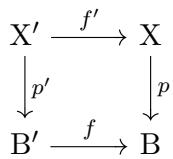
\includegraphics[keepaspectratio]{images/part001_94ec13ba.jpg}}

为一个笛卡尔方块。若映射 p 是分离的，则 p' 亦然。反之，若 p' 是分离的且 f 是普遍严格且满射的，则 p 是分离的。

考虑方块

\[
\begin{array}{c} \mathrm {X^ {\prime} \times_ {B^ {\prime}} X^ {\prime}} \xrightarrow {\varphi} \mathrm {X \times_ {B} X} \\ \Biggl \downarrow_ {q ^ {\prime}} \\ \mathrm {B^ {\prime} \xrightarrow {f} B} \end{array}
\]

其中映射 \(\varphi\) 由映射 \(f' \times f': X' \times X' \to X \times X\) 诱导。回顾 (I, p. 13, 例 1)，这个方块是笛卡尔的，并且有 \(\overline{\varphi}^1(\Delta_X) = \Delta_{X'}\) 。

若映射 p 是分离的，则集合 \(\Delta_{\mathrm{X}}\) 在 \(\mathrm{X} \times_{\mathrm{B}} \mathrm{X}\) 中是闭的；因此 \(\Delta_{\mathrm{X}'}\) 是 \(\mathrm{X}' \times_{\mathrm{B}'} \mathrm{X}'\) 的一个闭子集，这就证明了映射 \(p'\) 是分离的。

若映射 f 是满射的，则映射 \(\varphi\) 是满射的 (I, p. 10, cor.)；若 f 是普遍严格的，则 \(\varphi\) 是严格的 (I, p. 20, def. 6)。设映射 \(p'\) 是分离的。于是 \(\Delta_{\mathrm{X}'}\) 在 \(\mathrm{X}' \times_{\mathrm{B}'} \mathrm{X}'\) 中是闭的。由于 \(\Delta_{\mathrm{X}'} = \overline{\varphi}^{1}(\Delta_{\mathrm{X}})\) 且 \(\varphi\) 是满射且严格的，\(\Delta_{\mathrm{X}}\) 在 \(\mathrm{X} \times_{\mathrm{B}} \mathrm{X}\) 中是闭的，这就证明了映射 \(p\) 是分离的。

命题 5. --- 设 \(f: X \to Y\) 与 \(g: Y \to Z\) 为连续映射。设映射 \(g\) 是分离的且映射 \(g \circ f\) 是逆紧的。则映射 \(f\) 是逆紧的。

考虑下列笛卡尔方块：

\[
\begin{array}{c} \mathrm{X} \times_ {\mathrm{Z}} \mathrm{Y} \xrightarrow {\operatorname{pr} _ {2}} \mathrm{Y} \\ \Biggl \downarrow \operatorname{pr} _ {1} \\ \mathrm{X} \xrightarrow {g \circ f} \mathrm{Z}. \end{array}
\]

设 \(s \colon X \to X \times_{Z} Y\) 为映射 \(x \mapsto (x, f(x))\) 。它是 \(\mathrm{pr}_1 \colon X \times_{Z} Y \to X\) 的一个连续截面。由命题 4，映射 \(\mathrm{pr}_1\) 是分离的；由此推出映射 \(s\) 是逆紧的 (I, p. 27, prop. 3 与 TG, I, p. 72, prop. 2)。另一方面，映射 \(\mathrm{pr}_2\) 是逆紧的 (I, p. 17, prop. 8)。因此，映射 \(f\) （它等于 \(\mathrm{pr}_2 \circ s\) ）是逆紧的 (TG, I, p. 73, prop. 5)。

\subsection{平展映射}

定义 2. --- 设 E 与 B 为拓扑空间，\(p\colon\mathrm{E}\to\mathrm{B}\) 为一个映射，\(x\) 为 E 的一个点。我们称映射 \(p\) 在 \(x\) 处是拓扑平展的，如果存在 \(x\) 在 E 中的一个邻域 U 与 \(p(x)\) 在 B 中的一个邻域 V，使得 \(p\) 诱导出从 U 到 V 上的一个同胚。

我们称映射 p 是拓扑平展的，如果它在 E 的每个点 x 处都是拓扑平展的。

当不致产生混淆时 (cf. 下文例 3)，把拓扑平展简称为平展。代替说 \(p\colon \mathrm{E}\to \mathrm{B}\) 是一个平展映射，也可以说 B-空间 \((\mathrm{E},p)\) 是一个平展 B-空间，或者当映射 \(p\) 无疑问时，简单地说 E 是 B 上的一个平展空间。

注. --- 1) 使映射 \(p \colon \mathrm{E} \to \mathrm{B}\) 平展的 E 的点所成的集合是 E 的一个开子集 U，且 p 在 U 上的限制是一个从 U 到 B 的平展映射。

\begin{enumerate}
\def\labelenumi{\arabic{enumi})}
\setcounter{enumi}{1}
\tightlist
\item
  平展映射是连续且开的 (TG, I, p. 33, prop. 5)；特别地，平展映射的像是开的。反之，若 \(p \colon \mathrm{E} \to \mathrm{B}\) 是一个连续且开的映射，且 E 的每个点 x 都有一个邻域 V 使得映射 \(p \mid \mathrm{V}\) 是单射的，则映射 p 是平展的。平展映射的纤维是离散的。
\end{enumerate}

例. --- 1) 设 B 为一个拓扑空间，\((\mathrm{U}_{i})_{i\in\mathrm{I}}\) 为 B 的一族子集。设 E 表示族 \((\mathrm{U}_{i})_{i\in\mathrm{I}}\) 的和空间，\(p: E \to B\) 表示由诸 \(U_{i}\) 到 B 中的典型单射诱导的映射。为使映射 p 是平展的，必须且只需诸 \(U_{i}\) （\(i \in I\) ）都是开的。

\begin{enumerate}
\def\labelenumi{\arabic{enumi})}
\setcounter{enumi}{1}
\item
为使全纯函数 \(f\colon U \to \mathbf{C}\) 是一个平展映射，必须且只需它的导数不取零值。
\item
  代数簇的平展态射 (VAR, R, 5.7.8) 是一个拓扑平展映射，但存在实代数簇的态射，它是拓扑平展的而不是平展态射。例如，映射 \(x \mapsto x^3\) （从 \(\mathbf{R}\) 到 \(\mathbf{R}\) 中）就是这种情形。然而，一个拓扑平展的复解析簇的态射是平展态射 (I, p. 141, exerc. 6)。
\end{enumerate}

命题 6. — 设 X、Y、Z 为拓扑空间，\(f\colon X\to Y\) 、\(g\colon Y\to Z\) 为映射。

\begin{enumerate}
\def\labelenumi{\alph{enumi})}
\item
  设 f 与 g 都是平展的；则 \(g \circ f\) 是平展的。
\item
  设 \(g\) 是平展的，\(f\) 是连续的且 \(g \circ f\) 是开的。则 \(f\) 是开的。
\item
  设 \(g \circ f\) 与 \(g\) 是平展的，且 \(f\) 是连续的。则映射 \(f\) 是平展的。
\item
  设 \(g \circ f\) 是平展的且映射 \(f\) 是连续且开的；则 \(f\) 是平展的，且 \(g\) 在 \(f(\mathrm{X})\) 的每点处是平展的。
\end{enumerate}

我们来证明 (a)。设 \(f\) 与 \(g\) 都是平展的。于是它们都是连续且开的，从而映射 \(g \circ f\) 是连续且开的。设 \(x\) 为 X 的一个点。存在 \(f(x)\) 在 Y 中的一个邻域 W，使得 \(g \mid \mathrm{W}\) 是单射的，并且存在 \(x\) 在 X 中的一个邻域 V，它包含于 \(f(\mathrm{W})\) 中，使得 \(f \mid \mathrm{V}\) 是单射的；于是映射 \((g \circ f) \mid \mathrm{V}\) 是单射的。这就证明了映射 \(g \circ f\) 是平展的 (注 2)。

我们来证明 b)。设 x 为 X 的一个点，W 为 \(f(x)\) 的一个开邻域，使得 g 诱导出从 W 到开集 \(g(\mathrm{W})\) 上的一个同胚。设 V 为 x 的一个邻域，使得 \(f(\mathrm{V})\) 包含于 W 中；于是 \(g \circ f(\mathrm{V})\) 是 \(g \circ f(x)\) 的一个邻域，因此 \(f(\mathrm{V})\) 是 \(f(x)\) 在开集 W 中的一个邻域，从而也是在 Y 中的一个邻域。这就证明了映射 f 是开的 (TG, I, p. 33, prop. 5)。

我们来证明 c)。由 b)，f 是开的。设 x 为 X 的一个点。由于 \(g \circ f\) 是平展的，存在 x 在 X 中的一个邻域 V，使得 \(g \circ f \mid V\) 是单射的。于是 \(f \mid V\) 是单射的，且 f 是平展的 (I, p. 29, 注 2)。

我们来证明 d)。设 \(x\) 为 \(X\) 的一个点，并令 \(y = f(x)\) 。存在一个开邻域 \(V\) （\(x\) 的），使得 \(g \circ f\) 诱导出从 \(V\) 到开集 \(g \circ f(V)\) 上的一个同胚。由于映射 \(f\) 是开的，\(f(V)\) 是 \(y\) 的一个开邻域。映射 \(f|_V\colon V \to f(V)\) （由 \(f\) 过渡到子空间得到）是连续、开且双射的；因此它是一个同胚，从而 \(f\) 在 \(x\) 处是平展的。此外，映射 \(g\) 诱导出从 \(f(V)\) 到 \(g \circ f(V)\) 上的一个同胚，从而在 \(y\) 处是平展的。

推论 1. — 设 B 为一个拓扑空间。从一个平展 B-空间到另一个平展 B-空间的 B-态射是平展的。

这由命题 6 的断言 c) 得出。

推论 2. --- 设 B 为一个拓扑空间；从一个平展 B-空间到另一个平展 B-空间的双射 B-态射是一个 B-同构。

由推论 1，这样的态射是平展的；因此它是开的 (I, p. 29, 注 2)。若它是双射的，则它是一个 B-同构。

推论 3. --- 设 p: E → B 为一个平展映射。p 的每个连续截面都诱导出从 B 到 E 的一个开子集上的一个同胚。

事实上，这样的截面是平展的 (推论 1)，从而是开的。

推论 4. --- 设 p: E → B 为一个平展且分离的映射。设 E 是连通的且 p 有一个截面。则 p 是一个同胚。

设 \(s\) 为 \(p\) 的一个截面；由于 \(p\) 是平展的，\(s\) 的像在 E 中是开的 (推论 3)；它也是闭的，因为 \(p\) 是分离的 (I, p. 27, prop. 3)。由于 E 是连通的，我们有 \(s(\mathrm{B}) = \mathrm{E}\) ，从而 \(p\) 是一个同胚。

命题 7. --- 设 \(p\colon E \to B\) 为一个连续映射。为使映射 \(p\) 是平展的，必须且只需它是开的，且对角线 \(\Delta_{E}\) （\(E \times_{B} E\) 的）在 \(E \times_{B} E\) 中是开的。

首先设映射 p 是平展的。于是它是开的，且 E 的每个点都有一个邻域 V，使得 \(p|V\) 是单射的，这等于说 \((\mathrm{V} \times \mathrm{V}) \cap (\mathrm{E} \times_{\mathrm{B}} \mathrm{E}) \subset \Delta_{\mathrm{E}}\) 。因此 \(\Delta_{E}\) 是 \(E \times_{B} E\) 的一个开子集。

反之，设 p 是一个开映射且 \(\Delta_{\mathrm{E}}\) 是 \(\mathrm{E} \times_{\mathrm{B}} \mathrm{E}\) 的一个开子集。设 x 为 E 的一个点。设 V 为 x 在 E 中的一个开邻域，使得 \((\mathrm{V} \times \mathrm{V}) \cap (\mathrm{E} \times_{\mathrm{B}} \mathrm{E})\) 包含于 \(\Delta_{\mathrm{E}}\) 中。于是 \(p \mid \mathrm{V}\) 是单射的。由 I, p. 29 的注 2，映射 p 是平展的。

命题 8. --- 设

\pandocbounded{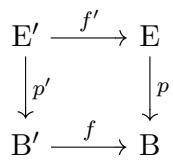
\includegraphics[keepaspectratio]{images/part001_e4ab0ebd.jpg}}

为一个笛卡尔方块。若态射 p 是平展的，则态射 p' 是平展的。反之，若态射 p' 是平展的且态射 f 是普遍严格且满射的，则态射 p 是平展的。

设映射 p 是平展的。特别地，它是开的，且 \(p'\) 是开的 (I, p. 17, prop. 8)。于是考虑笛卡尔方块 (I, p. 13, 例 1)

\[
\begin{array}{c} \mathrm{E} ^ {\prime} \times_ {\mathrm{B} ^ {\prime}} \mathrm{E} ^ {\prime} \xrightarrow {\varphi} \mathrm{E} \times_ {\mathrm{B}} \mathrm{E} \\ \Biggl \downarrow q ^ {\prime} \qquad \qquad \qquad \qquad \Biggl \downarrow q \\ \mathrm{B} ^ {\prime} \xrightarrow {f} \mathrm{B}. \end{array}
\]

我们有 \(\Delta_{\mathrm{E}^{\prime}} = \overline{\varphi}^{1}(\Delta_{\mathrm{E}})\) (loc. cit.)。此外，对角线 \(\Delta_{\mathrm{E}}\) 在 \(\mathrm{E} \times_{\mathrm{B}} \mathrm{E}\) 中是开的 (prop. 7)，从而对角线 \(\Delta_{\mathrm{E}^{\prime}}\) 在 \(\mathrm{E}^{\prime} \times_{\mathrm{B}^{\prime}} \mathrm{E}^{\prime}\) 中是开的。这就证明了映射 \(p^{\prime}\) 是平展的 (loc. cit.)。

现在设映射 \(f\) 是满射且普遍严格的，并设映射 \(p'\) 是平展的。于是 \(p'\) 是开的，因此 \(p\) 是开的 (I, p. 21, prop. 11, \(a\) )。另一方面，\(\Delta_{\mathrm{E}'}\) 是 \(\mathrm{E}' \times_{\mathrm{B}'} \mathrm{E}'\) 的一个开子集。由于 \(\Delta_{\mathrm{E}'} = \overline{\varphi}^{1}(\Delta_{\mathrm{E}})\) 且映射 \(\varphi\) 是满射且严格的 (I, p. 20, def. 6)，\(\Delta_{\mathrm{E}}\) 在 \(\mathrm{E} \times_{\mathrm{B}} \mathrm{E}\) 中是开的。由 prop. 7，映射 p 是平展的。

推论. --- 设 B 为一个拓扑空间。两个平展 B-空间的纤维积是一个平展 B-空间。

设 \((\mathrm{E}, p)\) 与 \((\mathrm{E}^{\prime}, p^{\prime})\) 为平展 B-空间。映射 \(pr_{1}: E \times_{B} E^{\prime} \to E\) 是平展的 (prop. 8)，从而映射 \(p \circ pr_{1}: E \times_{B} E^{\prime} \to B\) 是平展的 (prop. 6, a))。

注 3. --- 设

\pandocbounded{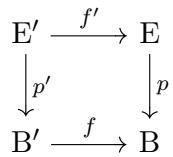
\includegraphics[keepaspectratio]{images/part001_b818a80c.jpg}}

为一个笛卡尔方块。若映射 p 是平展的且映射 f 是严格的，则映射 \(f'\) 是严格的。事实上，在这些假设之下，E 的每个点都有一个开邻域 U，使得 p 诱导出从 U 到开集 \(p(\mathrm{U})\) 上的一个同胚。于是映射 \(p'\) 诱导出从 \((f')^{-1}(\mathrm{U})\) 到 \(f^{-1}(p(\mathrm{U}))\) 上的一个同胚。映射 f 诱导出从 \(f^{-1}(p(\mathrm{U}))\) 到 \(p(\mathrm{U})\) 上的一个严格映射 (I, p. 20)，从而映射 \(f'\) 诱导出从 \((f')^{-1}(\mathrm{U})\) 到 U 中的一个严格映射。由此推出映射 \(f'\) 是严格的 (I, p. 23, 推论 2)。

\subsection{平展映射的局部截面}

设 E 与 B 为集合，A 为 B 的一个子集，\(p: E \rightarrow B\) 为一个映射。p 在 A 上的一个截面是一个映射 \(s: A \rightarrow E\) ，使得 \(p \circ s\) 是 A 到 B 中的典型单射。给出 p 在 A 上的一个截面 s，等价于给出由 p 诱导的映射 \(p_{\mathrm{A}} \colon \overline{p}^{1}(\mathrm{A}) \to \mathrm{A}\) 的一个截面。若 s 是 p 在 A 上的一个截面且 \(A'\) 是 A 的一个子集，则限制 \(s'\) （s 到 \(A'\) 上的）是 p 在 \(A'\) 上的一个截面。这时我们称 s 是 \(s'\) 到 A 上的一个延拓。

当 E 与 B 是拓扑空间且 \(p \colon \mathrm{E} \to \mathrm{B}\) 是连续映射时，集合 \(\mathcal{C}_{\mathrm{B}}(\mathrm{A};\mathrm{E})\) (I, p. 2)（即 \(p\) 在 A 上的连续截面所成的集合）也记作 \(\mathcal{S}(\mathrm{A};p)\) 或 \(\mathcal{S}(\mathrm{A};\mathrm{E})\) 。设 \(s\) 为 \(p\) 在 A 上的一个连续截面。映射 \(s\) 诱导出从 A 到 \(s(\mathrm{A})\) 上的一个同胚，而 \(p\) 诱导出其逆同胚。于是由 I, p. 28 的定义 2，我们有：

命题 9. --- 设 p: E → B 为一个连续映射。为使 p 是平展的，必须且只需 E 的每个点都有一个开邻域，它是在 B 的某个开子集上定义的 p 的一个连续截面的像。

注. --- 1) 设 \(p \colon \mathrm{E} \to \mathrm{B}\) 为一个连续且开的映射。为使 E 的一个开集 U 是 \(p\) 在 B 的某个开集上的一个连续截面的像，必须且只需 \(p\) 在 U 上的限制是单射的。

\begin{enumerate}
\def\labelenumi{\arabic{enumi})}
\setcounter{enumi}{1}
\tightlist
\item
  设 \(p \colon \mathrm{E} \to \mathrm{B}\) 为一个连续映射。设 B 的每个点都有一个开邻域 V，使得存在 \(p\) 在 V 上的一个连续截面。这样的映射 \(p\) 未必是平展的，甚至未必是开的。然而它是满射且普遍严格的 (I, p. 20, 推论)。
\end{enumerate}

\subsection{平展映射的连续提升}

设 \(p \colon \mathrm{E} \to \mathrm{B}\) 与 \(f \colon \mathrm{Z} \to \mathrm{B}\) 为连续映射。\(f\) 到 \(\mathrm{E}\) 中的一个连续提升是指一个连续映射 \(g \colon \mathrm{Z} \to \mathrm{E}\) ，使得 \(p \circ g = f\) 。\(f\) 到 \(\mathrm{E}\) 中的连续提升所成的集合不是别的，正是 \(\mathcal{C}_{\mathrm{B}}(\mathrm{Z};\mathrm{E})\) 。它也可以等同于集合 \(\mathcal{S}(\mathrm{Z};\mathrm{Z} \times_{\mathrm{B}}\mathrm{E})\) ，即 Z-空间 \((\mathrm{Z} \times_{\mathrm{B}}\mathrm{E},\mathrm{pr}_{1})\) 的投影的连续截面所成的集合。

若 T 是 Z 的一个子集，则 f 到 E 中的一个在 T 上定义的连续提升称为 f \textbar{} T 到 E 中的一个连续提升：

\pandocbounded{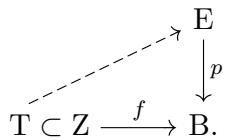
\includegraphics[keepaspectratio]{images/part001_46887bc2.jpg}}

命题 10. --- 设 E、B 与 Z 为拓扑空间，\(p\colon E \to B\) 为一个平展映射，\(f\colon Z \to B\) 为一个连续映射。

设 \(z \in \mathbf{Z}\) 与 \(x \in \mathrm{E}\) 为满足 \(f(z) = p(x)\) 的点。存在一个邻域 \(\mathrm{W}\) （\(z\) 的，在 \(\mathbf{Z}\) 上），以及一个连续提升 \(g\) （\(f\) 的，到 \(\mathrm{E}\) 中），它在 \(\mathrm{W}\) 上定义且满足 \(g(z) = x\) 。

存在 \(p(x)\) 在 B 中的一个开邻域 V 以及 p 在 V 上的一个连续截面 s，使得 \(s(p(x)) = x\) (命题 9)。集合 \(W = f^{-1}(V)\) 是 z 的一个开邻域，而映射 \(g = s \circ (f|W)\) 是 f 到 E 中的一个连续提升，它在 W 上定义且满足 \(g(z) = x\) 。

命题 11. --- 设 E、B 与 Z 为拓扑空间，\(p\colon E \to B\) 与 \(f\colon Z \to B\) 为连续映射。设 \(g\) 与 \(g'\) 为 \(f\) 到 E 中的连续提升。设 W 为 Z 中使 \(g\) 与 \(g'\) 相等的点所成的集合。

\begin{enumerate}
\def\labelenumi{\alph{enumi})}
\item
  若映射 p 是分离的，则 W 是闭的。
\item
  若映射 p 是平展的，则 W 是开的。
\end{enumerate}

用 \(h\) 表示连续映射 \((g, g')\colon Z \to E \times E\) 。\(h\) 的像包含于 \(E \times_{B} E\) 中，因为 \(p \circ g = f = p \circ g'\) ，而 Z 中使 g 与 g' 相等的点所成的集合 W，就是 \(h\) 之下对角线 \(\Delta_{E}\) 的原像。

若映射 p 是平展的，则对角线 \(\Delta_{E}\) 在 \(E \times_{B} E\) 中是开的 (I, p. 31, prop. 7)，从而集合 W 在 Z 中是开的。

若映射 p 是分离的，则对角线 \(\Delta_{E}\) 在 \(E \times_{B} E\) 中是闭的 (I, p. 25, def. 1)，从而集合 W 在 Z 中是闭的。

推论 1. --- 若空间 Z 是连通的且映射 p 是平展且分离的，则在某一点相等的 f 到 E 中的连续提升都相等。

推论 2. --- 设 \(p\colon E \to B\) 为一个分离的平展映射。若空间 E 是连通的，则群 \(\mathrm{Aut}_{\mathrm{B}}(\mathrm{E})\) 自由地作用在 E 上。

事实上，若 \(f: \mathrm{E} \to \mathrm{E}\) 是一个 B-态射，则由推论 1，f 与 \(\mathrm{Id}_{\mathrm{E}}\) 相等的点所成的集合是 E 或空集。

推论 3. --- 设 E、B 与 Z 为拓扑空间，\(p\colon E \to B\) 为一个分离的平展态射，\(f\colon Z \to B\) 为一个连续映射。对 \(i = 1,2\) ，设 \(U_i\) 为 Z 的一个开（相应地，闭）子集，\(g_i\colon U_i \to E\) 为 f 的一个在 \(U_i\) 上定义的连续提升。假设交 \(U_1 \cap U_2\) 是连通的，且存在 \(U_1 \cap U_2\) 的一个点 z，使得 \(g_1(z) = g_2(z)\) 。则存在 f 的一个在 \(U_1 \cup U_2\) 上定义的连续提升，它是 \(g_1\) 与 \(g_2\) 的延拓。

由推论 1，在 \(U_{1} \cap U_{2}\) 上，\(g_{1}\) 与 \(g_{2}\) 的限制相等。映射 \(g: U_{1} \cup U_{2} \to E\) ——由 \(g(z) = g_{i}(z)\) （对 \(z \in U_{i}\) ，i = 1, 2）定义——是 f 的一个在 \(U_{1} \cup U_{2}\) 上定义的连续提升 (TG, I, p. 19, prop. 4)。

在前面的结果中，Z = B 且 \(f = Id_{B}\) 的特殊情形是重要的：这时 f 的连续提升就是 p 的连续截面。

命题 12. --- 设 \(p \colon E \to B\) 为一个平展映射。为使映射 \(p\) 是分离的，必须且只需：对每个开子集 \(V\) （\(B\) 的）与每对 \((s, s')\) （\(p\) 在 \(V\) 上的连续截面的对），使 \(s\) 与 \(s'\) 相等的点所成的集合在 \(V\) 中是闭的。

该条件是必要的 (命题 11, I, p. 34)。我们来证明它是充分的。设 \(b\) 为 B 的一个点，并设 \(x\) 与 \(x'\) 为 E 的两个不同的点，满足 \(p(x) = p(x') = b\) 。设 V 为 b 的一个开邻域，s 与 s' 为 p 在 V 上的连续截面，使得 \(s(\mathrm{V})\) 与 \(s'(\mathrm{V})\) 分别是 x 与 x' 的开邻域 (命题 9)。按假设，由点 \(x \in \mathrm{V}\) （满足 \(s(x) \ne s'(x)\) ）组成的集合 W 在 V 中是开的，从而在 B 中也是开的。集合 \(s(\mathrm{W})\) 与 \(s'(\mathrm{W})\) 分别是 x 与 x' 的开邻域；它们按构造是不相交的。这就证明了映射 p 是分离的 (I, p. 25, 定义 1)。

\subsection{平展映射的连续截面的构造}

定理 1. --- 设 X、Y、Z 为拓扑空间，\(f: \mathrm{Z} \to \mathrm{X} \times \mathrm{Y}\) 为一个分离平展态射，并设 \(y_0\) 为 Y 的一点。设 \(s: X \times Y \to Z\) 为 \(f\) 的一个截面。假定 \(s\) 在 \(X \times \{y_0\}\) 上的限制是连续的，并且 \(s\) 在 \(\{x\} \times Y\) （对每个 \(x \in X\) ）上的限制也都是连续的。若空间 \(Y\) 是连通且局部连通的 (TG, I, p. 84, def. 4)，则映射 \(s\) 是连续的。

引理. --- 设 U 为 X 的一个开子集，V 为 Y 的一个连通开子集，并设 \((x_{1},y_{1})\in\mathrm{U}\times\mathrm{V}\) 。假定 s 在 \(U\times\{y_{1}\}\) 上的限制是连续的。设 \(\sigma\) 为 f 在 \(U\times V\) 上的一个连续截面，使得 \(\sigma(x_{1},y_{1})=s(x_{1},y_{1})\) 。则存在一个邻域 \(U'\) （\(x_{1}\) 的），使得 \(s=\sigma\) 在 \(U'\times V\) 上成立。特别地，映射 s 在 \((x_{1},y_{1})\) 的一个邻域中是连续的。

由于 \(s\) 在 \(\mathrm{U} \times \{y_1\}\) 上的限制是连续的，且映射 \(f\) 是平展的，故存在一个邻域 \(\mathrm{U}'\) （\(x_1\) 的），使得 \(s(x, y_1) = \sigma(x, y_1)\) 对一切 \(x \in \mathrm{U}'\) 成立 (I, p. 34, prop. 11, b))。设 \(x \in \mathrm{U}'\) ；由于 \(s\) 在 \(\{x\} \times \mathrm{V}\) 上的限制是连续的，且映射 \(f\) 是平展且分离的，由 I, p. 34 的推论 1 得出，\(\sigma(x, y) = s(x, y)\) 对一切 \(y \in \mathrm{V}\) 成立。于是，\(s\) 与 \(\sigma\) 在 \(\mathrm{U}' \times \mathrm{V}\) 上重合。

现在来证明定理。首先证明映射 s 在 \(X \times \{y_{0}\}\) 的每一点的一个邻域中是连续的。设 \(x_{0} \in X\) ；可以选取 X 中 \(x_{0}\) 的一个开邻域 U、Y 中 \(y_{0}\) 的一个连通开邻域 V，以及 f 的一个连续截面 \(\sigma: U \times V \to Z\) ，使得 \(\sigma(x_{0}, y_{0}) = s(x_{0}, y_{0})\) 。由上述引理，s 在 \((x_{0}, y_{0})\) 的一个邻域中是连续的。

我们现证明映射 \(s\) 在 \(\mathrm{X} \times \mathrm{Y}\) 的每一点处都是连续的。对 \(x_0 \in \mathrm{X}\) ，用 \(\mathrm{C}(x_0)\) 表示点 \(y \in \mathrm{Y}\) （使 \(s\) 在 \((x_0, y)\) 的一个邻域中连续者）所成的集。按定义，集 \(\mathrm{C}(x_0)\) 在 Y 中是开的，且由前所证它含有 \(y_0\) 。

我们来证明它在 Y 中是闭的。考虑 Y 中的一点 \(y_{1}\) （属于 \(\mathrm{C}(x_{0})\) 的闭包者）、X 中 \(x_{0}\) 的一个开邻域 U、Y 中 \(y_{1}\) 的一个开邻域 V，以及 f 的一个连续截面 \(\sigma\colon U\times V\to Z\) ，使得 \(\sigma(x_{0},y_{1})=s(x_{0},y_{1})\) 。由于 s 在 \(\{x_{0}\}\times V\) 上的限制连续且 f 是平展的，故存在一个开邻域 \(V^{\prime}\) （\(y_{1}\) 的，在 Y 中），使得 \(\sigma(x_{0},y)=s(x_{0},y)\) 对一切 \(y\in V^{\prime}\) 成立 (I, p. 34 的命题 11)。由于 Y 是局部连通的，可以假设 \(V^{\prime}\) 是连通的。由于 \(y_{1}\) 属于 \(\mathrm{C}(x_{0})\) 的闭包，集 \(\mathrm{C}(x_{0})\cap\mathrm{V}^{\prime}\) 非空；设 \(y_{2}\) 为 \(\mathrm{C}(x_{0})\cap\mathrm{V}^{\prime}\) 的一点。把引理应用于 \((x_{0},y_{2})\) ，便存在一个邻域 \(U^{\prime}\) （\(x_{0}\) 的，含于 U 中），使得 \(s=\sigma\) 在 \(U^{\prime} \times V^{\prime}\) 上成立。这就证明了 \(\mathrm{C}(x_{0})\) 是闭的，因为 \(U^{\prime} \times V^{\prime}\) 是 \((x_{0}, y_{1})\) 的一个邻域。由于 Y 是连通的，我们有 \(\mathrm{C}(x_{0}) = \mathrm{Y}\) ，且这对每个 \(x_{0} \in X\) 都成立，由此即得定理。

推论 1. --- 设 X、Y、E、B 为拓扑空间。设 \(p\colon E \to B\) 为一个平展且分离的映射，\(h\colon X \times Y \to B\) 为一个连续映射，并设 \(y_0\) 为 Y 的一点。设 \(g\colon X \times Y \to E\) 为满足 \(p \circ g = h\) 的一个映射。假设 \(g\) 在 \(X \times \{y_0\}\) 上的限制以及，对每个 \(x \in X\) ，在 \(\{x\} \times Y\) 上的限制都是连续的。若空间 Y 是连通且局部连通的，则映射 \(g\) 是连续的。

设 Z 为纤维积 \((\mathrm{X} \times \mathrm{Y}) \times_{\mathrm{B}} \mathrm{E}\) ，并设 \(f: Z \to X \times Y\) 与 \(h': Z \to E\) 为典范投影。映射 f 是平展的 (I, p. 31, prop. 8) 且是分离的 (I, p. 27, prop. 4)。映射 \(s: X \times Y \to Z\) （由 \(s(x, y) = ((x, y), g(x, y))\) 定义）是 f 的一个截面，它满足定理 1 的诸假设。因此它是连续的，\(g = h' \circ s\) 亦然。

注. --- 若在定理 1 中不假设空间 Y 是局部连通的，则定理的结论不再必然成立 (I, p. 141, exerc. 7)。

定理 2. --- 设 B 为一个拓扑空间，A 为 B 的一个子空间。假设下列假设之一成立：

\begin{enumerate}
\def\labelenumi{(\roman{enumi})}
\item
  A 具有由仿紧邻域组成的基本邻域系；
\item
  B 是仿紧的且 A 是闭的；
\item
  B 是可度量化的；
\item
  A 是紧的，且 A 中任意两个不同的点在 B 中有不相交的邻域。
\end{enumerate}

那么，平展映射 \(p\colon E \to B\) 在 A 上的每个连续截面都可以扩张为 \(p\) 在 A 的一个邻域上的连续截面。

考虑数对 (B, A) 的下列性质 (PCV)：

(PCV) 对由 B 的开子集组成的 A 的每个覆盖 \((\mathrm{U}_{i})_{i\in\mathrm{I}}\) ，存在 A 的一个邻域 V 和覆盖 V 的、由 V 的闭子集组成的局部有限族 \((\mathrm{F}_{j})_{j\in\mathrm{J}}\) ，使得每个 \(F_{j}\) 都含于某个 \(U_{i}\) 之中。

定理 2 由下文的引理 1 与引理 3 得出。

引理 1. --- 定理 2 的性质 (i) 至 (iv) 中的每一条都蕴涵性质 (PCV)。

设 \((\mathrm{U}_{i})_{i\in\mathrm{I}}\) 为由 B 的开子集组成的 A 的一个覆盖。在假设 (i) 之下，存在 A 的一个仿紧邻域 V，它含于诸 \(U_{i}\) 的并，存在空间 V 的一个开覆盖 \((\mathrm{U}_{j}^{\prime})_{j\in\mathrm{J}}\) ，它是局部有限的且加细于覆盖 \((\mathrm{V}\cap\mathrm{U}_{i})_{i\in\mathrm{I}}\) ，还存在空间 V 的一个开覆盖 \((\mathrm{U}_{j}^{\prime\prime})_{j\in\mathrm{J}}\) ，使得对每个 \(j\in J\) ，闭包 \(F_{j}\) （\(U_{j}^{\prime\prime}\) 在 V 中的）含于 \(U_{j}^{\prime}\) (TG, IX, p. 49, prop. 4 及 p. 48, th. 3 的 cor. 1)。故在此情形下 (PCV) 成立。

由 TG, IX, p. 50 的推论 2，条件 (ii) 蕴涵条件 (i)。同样，条件 (iii) 蕴涵条件 (i)：事实上，若 B 是可度量化的，则 A 的每个邻域都是可度量化的，从而是仿紧的 (TG, IX, p. 51, th. 4)。

最后假设条件 (iv) 成立，我们来证明性质 (PCV) 成立。由于 A 是紧的，只需考虑有限覆盖 \((\mathrm{U}_{i})_{0\leqslant i\leqslant n}\) 的情形。于是用归纳法构造 B 的开集 \(V_{0},\ldots,V_{n}\) ，使其对 \(0\leqslant i\leqslant n\) 满足下列条件：

\(\alpha)\mathrm{A}\subset \mathrm{V}_{0}\cup \dots \cup \mathrm{V}_{i}\cup \mathrm{U}_{i + 1}\cup \dots \cup \mathrm{U}_{n};\)

\(\beta)\overline{\mathrm{V}_{i}}\cap \mathrm{A}\subset \mathrm{U}_{i}.\)

设 \(V_{0},\ldots,V_{r-1}\) 已经构造出来，且对 \(0\leqslant i\leqslant r-1\) 满足上述条件，而来构造 \(V_{r}\) 。集合 \(K=A\cap C U_{r}\) 与 \(L=A\cap C(V_{0}\cup\cdots\cup V_{r-1}\cup U_{r+1}\cup\cdots\cup U_{n})\) 在 A 中是闭的，因而是紧的。根据 \((\alpha)\) ，它们不相交。由假设，对 L 的每一点 a 与 K 的每一点 b，存在 a 与 b 在 B 中的不相交邻域。由下文的引理 2，存在 B 中的开集 \(V_{r}\) 与 W，二者不相交，且 \(L\subset V_{r}\) 与 \(K\subset W\) 。由包含关系 \(L\subset V_{r}\) 与 \(A\subset V_{0}\cup\cdots\cup V_{r-1}\cup U_{r}\cup\cdots\cup U_{n}\) 以及 L 的定义，可对 i=r 推出 \((\alpha)\) 。另一方面，有 \(\overline{V_{r}}\cap K=\varnothing\) ，从而 \(\overline{V_{r}}\cap A\subset U_{r}\) 。

集合 \(M = \bigcup_{0 \leqslant i \leqslant n} (\overline{\mathrm{V}_{i}} \cap \mathbb{C}\mathrm{U}_{i})\) 是闭的，且由 \(\beta\) 知它与 A 不相交。由 \(\alpha\) ，集合 \(V = (\bigcup_{0 \leqslant i \leqslant n} \overline{\mathrm{V}_{i}}) - M\) 是 A 在 B 中的一个邻域。对 \(i = 0, \ldots, n\) ，令 \(F_{i} = V \cap \overline{V_{i}}\) ；它是 V 的一个闭子集，含于 \(U_{i}\) 。族 \((F_{i})_{0 \leqslant i \leqslant n}\) 是 V 的一个覆盖，故性质 (PCV) 成立。

引理 2. --- 设 B 为一个拓扑空间，并设 K 与 L 为 B 的拟紧子集。假设对 K 的每一点 a 与 L 的每一点 b，存在 a 与 b 在 B 中的不相交邻域。那么存在 B 中两个不相交的开集 U 与 V，使得 K ⊂ U 且 L ⊂ V。

设 \(a\) 为 K 的一点。对每个 \(b \in L\) ，设 \(U_{a,b}\) 与 \(V_{a,b}\) 分别为 \(a\) 与 \(b\) 的不相交开邻域。固定 \(a\) ，族 \((V_{a,b})_{b \in L}\) 是 L 的一个开覆盖。由于 L 是拟紧的，存在一个有限族 \(T_a \subset L\) ，使得 \(V_b\) （诸 \(V_{a,b}\) 对 \(b \in T_a\) 者的并）包含 L。交 \(U_a\) （诸 \(U_{a,b}\) 对 \(b \in T_a\) 者之交）是 \(a\) 的一个开邻域，因为 \(T_a\) 是有限的；此外，\(U_a\) 与 \(V_a\) 不相交。诸 \((U_a)_{a \in A}\) 构成 K 的一个开覆盖。由于 K 是拟紧的，存在一个有限族 \(S \subset K\) ，使得 \(U = \bigcup_{a \in S} U_a\) 包含 K。于是，\(V = \bigcap_{a \in S} V_a\) 是 B 的一个包含 L 的开子集。引理得证。

引理 3. --- 设 B 为一个拓扑空间，A 为 B 的一个子空间，使得数对 (B,A) 满足 I, p. 37 的性质 (PCV)。那么，平展映射 \(p\colon E \to B\) 在 A 上的每个连续截面都可以扩张为 \(p\) 在 A 的一个邻域上的连续截面。

设 \(p \colon \mathrm{E} \to \mathrm{B}\) 为一个平展映射，\(s \colon \mathrm{A} \to \mathrm{E}\) 为 \(p\) 在 A 上的一个连续截面。对 A 的每一点 \(a\) ，存在一个开邻域 \(\mathrm{U}_a\) （\(a\) 的）和一个连续截面 \(s_a \colon \mathrm{U}_a \to \mathrm{E}\) ，它与 \(s\) 在 \(\mathrm{U}_a \cap \mathrm{A}\) 上重合 (I, p. 34, prop. 10 及 I, p. 34, prop. 11)。族 \((\mathrm{U}_a)_{a \in \mathrm{A}}\) 是由 B 的开集组成的 A 的一个覆盖。设 V 为 A 在 B 中的一个邻域，\((\mathrm{F}_j)_{j \in \mathrm{J}}\) 为覆盖 V 的、由 V 的闭子集组成的局部有限族，并设 \(a \colon \mathrm{J} \to \mathrm{A}\) 为一个映射，使得 \(\mathrm{F}_j\) 含于 \(\mathrm{U}_{a(j)}\) （对一切 \(j \in \mathrm{J}\) ；性质 (PCV)）。用 \(s_j\) 表示 \(s_{a(j)}\) 在 \(\mathrm{F}_j\) 上的限制。设 W 为满足下列条件的点 \(b \in \mathrm{V}\) 所成的集：\(s_j(b) = s_k(b)\) 对每对 \((j, k) \in \mathrm{J} \times \mathrm{J}\) （使 \(b \in \mathrm{F}_j \cap \mathrm{F}_k\) 者）都成立。我们定义截面 \(s' \colon \mathrm{W} \to \mathrm{E}\) 如下：\(s'(b) = s_j(b)\) （若 \(b \in \mathrm{F}_j\) ）。我们有 \(\mathrm{A} \subset \mathrm{W}\) 且 \(s' | \mathrm{A} = s\)。由 I, p. 19 的 prop. 4，截面 \(s'\) 是连续的。

尚须证明 W 是 A 在 B 中的一个邻域。对每对 \((j,k)\in\mathrm{J}\times\mathrm{J}\) ，用 \(T_{jk}\) 表示点 \(b\in F_{j}\cap F_{k}\) （满足 \(s_{j}(b)\neq s_{k}(b)\) 者）所成的集。集 \(T_{jk}\) 在 \(F_{j}\cap F_{k}\) 中是闭的 (I, p. 34 的 prop. 11, b))，从而在 V 中是闭的，且诸集 \(T_{jk}\) 构成 V 的子集的一个局部有限族。于是族 \((T_{jk})\) 之并 T 是 V 中的一个闭集 (TG, I, p. 6, prop. 4)。而按定义，W 是 T 在 V 中的余集。因此它是 A 在 V 中的一个邻域，从而也是 A 在 B 中的邻域。

\subsection{平展且分离映射的纤维基数的上界}

定理 3. --- 设 E 与 B 为拓扑空间，p: E → B 为一个平展且分离的映射。假设 E 是连通的，且 B 是局部连通的。设 W 为 B 的拓扑的一个基。那么，对 B 的每一点 a，有 Card(E \(_{a}\) ) ≤ sup(Card(W), Card(N))。

由于空间 B 是局部连通的，它的拓扑有一个由连通开集组成的基 \(\mathcal{W}'\) ，例如诸开集 \(\mathcal{W}\) 的连通分支 (TG, I, p. 85, prop. 11)。根据下文的引理 4，存在由连通开集组成的 B 的拓扑的一个基 \(\mathcal{V}\) ，且满足 \(\mathrm{Card}(\mathcal{V}) \leqslant \mathrm{Card}(\mathcal{W})^2\) 。

引理 4. --- 设 B 为一个拓扑空间，并设 W 与 W' 为 B 的拓扑的基。存在 W' 的一个子集 V，它是 B 的拓扑的一个基，且满足 \(\text{Card}(\mathcal{V}) \leqslant \text{Card}(\mathcal{W})^{2}\) 。

设 \(\mathcal{A} \subset \mathcal{W} \times \mathcal{W}\) 为如下的对 \((\mathrm{W}_1, \mathrm{W}_2)\) 所成的集：存在 \(\mathrm{W}' \in \mathcal{W}'\) 使 \(\mathrm{W}_1 \subset \mathrm{W}' \subset \mathrm{W}_2\) ；设 \(\varphi: \mathcal{A} \to \mathcal{W}'\) 为一个映射，使得 \(\mathrm{W}_1 \subset \varphi(\mathrm{W}_1, \mathrm{W}_2) \subset \mathrm{W}_2\) 对每个对 \((\mathrm{W}_1, \mathrm{W}_2) \in \mathcal{A}\) 成立，并设 \(\mathcal{V} \subset \mathcal{W}'\) 为 \(\varphi\) 的像。我们有

\[
\operatorname{Card} (\mathcal {V}) \leqslant \operatorname{Card} (\mathcal {A}) \leqslant \operatorname{Card} (\mathcal {W} \times \mathcal {W})
\]

(E, III, p. 25, prop. 3)。我们来证明 V 是 B 的拓扑的一个基。设 x 为 B 的一点，U 为 x 的一个邻域。由假设，x 有一个邻域 \(W_{2} \in W\) 含于 U，有一个邻域 \(W' \in W'\) 含于 \(W_{2}\) ，且有一个邻域 \(W_{1} \in W\) 含于 \(W'\) 。于是有 \(W_{1} \subset W' \subset W_{2} \subset U\) 。那么，\((W_{1}, W_{2}) \in \mathscr{A}\) ，且 \(\varphi(W_{1}, W_{2})\) 是 x 的一个含于 U 的邻域。根据 TG, I, p. 5 的 prop. 3，集 V 是 B 的拓扑的一个基。

设 V 为由非空连通开集组成的 B 的拓扑的一个基，且满足 \(\text{Card}(\mathcal{V}) \leqslant \text{Card}(\mathcal{W})^{2}\) 。设 U 为 E 的如下的开集 U 所成的集：p 诱导从 U 到属于 V 的某个开集 V 上的一个同胚。U 的每个元素都是非空连通开集。由于映射 p 是平展的，根据定义 2 (I, p. 28) 与 TG, I, p. 5 的 prop. 3，集 U 是 E 的拓扑的一个基。我们把 U 的元素的每个有限序列 \((\mathrm{U}_{0}, \ldots, \mathrm{U}_{n})\) 称为毛虫，如果对 \(1 \leqslant i \leqslant n\) ，\(U_{i-1} \cap U_{i}\) 非空且 \(p(\mathrm{U}_{i-1}) \cap p(\mathrm{U}_{i})\) 连通。用 S 表示 V 的元素的有限序列所成的集，并对每个毛虫 \(c = (\mathrm{U}_{0}, \ldots, \mathrm{U}_{n})\) ，用 \(p(c)\) 表示序列 \((p(\mathrm{U}_{0}), \ldots, p(\mathrm{U}_{n}))\) 。

引理 5. --- a) 设 \(c = (\mathrm{U}_0, \ldots, \mathrm{U}_n)\) 与 \(c' = (\mathrm{U}_0', \ldots, \mathrm{U}_m')\) 为两个毛虫，满足 \(\mathrm{U}_0 = \mathrm{U}_0'\) 且 \(p(c) = p(c')\) 。那么 \(c = c'\) 。

\begin{enumerate}
\def\labelenumi{\alph{enumi})}
\setcounter{enumi}{1}
\item
  设 U 与 U' 为 U 的元素。则存在一个毛虫 \(c = (\mathrm{U}_{0}, \ldots, \mathrm{U}_{n})\) ，使得 \(U_{0} = U\) 且 \(U_{n} = U'\) 。
\item
  必然有 m = n。对每个满足 \(0 \leqslant i \leqslant n\) 的整数 i，令 \(V_{i} = p(U_{i})\) ，并用 \(s_{i}\) 与 \(s_{i}^{\prime}\) 表示 p 在 \(V_{i}\) 上的、其像分别为 \(U_{i}\) 与 \(U_{i}^{\prime}\) 的连续截面。为证等式 \(c = c^{\prime}\) ，我们对 i 用归纳法证明等式 \(s_{i} = s_{i}^{\prime}\) （对每个满足 \(0 \leqslant i \leqslant n\) 的整数 i 成立）。由假设，有 \(s_{0} = s_{0}^{\prime}\) 。设 i 满足 \(1 \leqslant i \leqslant n\) 且 \(s_{i-1} = s_{i-1}^{\prime}\) 。由于 \(U_{i-1} \cap U_{i}\) 含有一点 x，连续截面 \(s_{i-1}\) 与 \(s_{i}\) 在 \(p(x)\) 处重合，从而在 \(V_{i-1} \cap V_{i}\) 的每一点处重合，因为它是连通的 (I, p. 34 的推论 1)。对 \(s_{i-1}^{\prime}\) 与 \(s_{i}^{\prime}\) 同理。出于同样的理由，\(s_{i}\) 与 \(s_{i}^{\prime}\) （在 \(V_{i-1} \cap V_{i}\) 中重合者）也在 \(V_{i}\) 中重合，由此即得结论。
\item
  若 \(x\) 与 \(y\) 为 E 的点，则称毛虫 \(c = (\mathrm{U}_0, \ldots, \mathrm{U}_n)\) 连接 \(x\) 到 \(y\) ，如果 \(x \in \mathrm{U}_0\) 且 \(y \in \mathrm{U}_n\) 。在集合 E 中，设 R 为关系“存在连接 \(x\) 到 \(y\) 的毛虫”。关系 R 是自反的，因为 \(\mathcal{U}\) 是 E 的一个覆盖。它显然是对称的。我们来证明它是传递的：设 \(x, y, z\) 为 E 的三点，\((\mathrm{U}_0, \ldots, \mathrm{U}_n)\) 与 \((\mathrm{U}_0', \ldots, \mathrm{U}_m')\) 为分别连接 \(x\) 到 \(y\) 与 \(y\) 到 \(z\) 的毛虫。设 \(\mathrm{U} \in \mathcal{U}\) 为 \(y\) 的一个含于 \(\mathrm{U}_n \cap \mathrm{U}_0'\) 的邻域；我们有 \(p(\mathrm{U}_n) \cap p(\mathrm{U}) = p(\mathrm{U}_0') \cap p(\mathrm{U}) = p(\mathrm{U})\) ，且由于 U 连通，序列 \((\mathrm{U}_0, \ldots, \mathrm{U}_n, \mathrm{U}, \mathrm{U}_0', \ldots, \mathrm{U}_m')\) 是连接 \(x\) 到 \(z\) 的毛虫。R 的等价类都是开的，从而也是闭的。由于 E 是连通的，由此得出 E 的任意两点总可由一条毛虫连接。
\end{enumerate}

设 U 与 U′ 为 U 的元素，x 为 U 的一点，\(x'\) 为 U' 的一点。存在一个毛虫 \((\mathrm{U}_{2},\ldots,\mathrm{U}_{n-2})\) ，它连接 x 到 \(x'\) 。设 \(U_{1}\) 与 \(U_{n-1}\) 为 U 的开子集，使得 \(x \in U_{1}\) 、\(x' \in U_{n-1}\) 、\(U_{1} \subset U \cap U_{2}\) 、\(U_{n-1} \subset U' \cap U_{n-2}\) 。令 \(U_{0} = U\) ，\(U_{n} = U'\) 。那么序列 \((\mathrm{U}_{0},\ldots,\mathrm{U}_{n})\) 是一个毛虫。

现在来证明定理。设 U 为 \(\mathcal{U}\) 的一个元素，并设 C 为毛虫 \((\mathrm{U}_0,\dots ,\mathrm{U}_n)\) （满足 \(\mathrm{U}_0 = \mathrm{U}\) 者）所成的集。把 C 中的毛虫 \(c = (\mathrm{U}_0,\dots ,\mathrm{U}_n)\) 映为序列 \(p(c) = (p(\mathrm{U}_{0}), \ldots, p(\mathrm{U}_{n}))\) 的、从 C 到 S 的映射是单射（引理 5, (a)），从而有 (1) \(\text{Card}(\mathrm{C}) \leqslant \text{Card}(\mathrm{S}).\)

从 C 到 \(\mathcal{U}\) 的、把 \(c = (\mathrm{U}_0,\dots ,\mathrm{U}_n)\in \mathrm{C}\) 映为开集 \(\mathrm{U}_n\) 的映射是满射（由引理 5 的第二部分），从而

\[
\operatorname{Card} (\mathcal {U}) \leqslant \operatorname{Card} (\mathrm{C}).\tag{2}
\]

对 E 的每一点 \(x\) ，选取开集 \(\mathrm{U}_x\) （\(\mathcal{U}\) 中的），使得 \(x \in \mathrm{U}_x\) 。若 \(x\) 与 \(y\) 是同一纤维 \(\mathrm{E}_a\) （\(p\) 的）中的不同点，则有 \(\mathrm{U}_x \neq \mathrm{U}_y\) ，因为 \(p \mid \mathrm{U}_x\) 是单射。于是，对 \(a \in \mathrm{B}\) ，我们有

\[
\operatorname{Card} \left(\mathrm{E} _ {a}\right) \leqslant \operatorname{Card} (\mathcal {U}).\tag{3}
\]

最后，若 V 是有限集，则 V 的元素的有限序列所成的集 S 是可数的 (E, III, p. 49, prop. 1)，从而

\[
\operatorname{Card} (\mathrm{S}) \leqslant \operatorname{Card} (\mathbf {N}).\tag{4}
\]

若 \(\mathcal{V}\) 是无限的，我们有

\[
\operatorname{Card} (\mathrm{S}) = \operatorname{Card} (\mathcal {V}) \leqslant \operatorname{Card} (\mathcal {W}) ^ {2} = \operatorname{Card} (\mathcal {W})\tag{5}
\]

由 E, III, p. 50 的推论与 E, III, p. 49 的推论 1 即得。定理由上述关系式 (1) 至 (5) 得出。

注. --- 由前所证，若 B 的拓扑有可数基，则 E 的拓扑亦有可数基，且 E 的纤维是可数的（参看 TG, I, p. 88, Poincaré-Volterra 定理）。

\section{层}

\subsection{集合的层}

设 B 为一个拓扑空间。

定义 1. --- B 上的、相对于 B 的拓扑的一个基 \(\mathcal{B}\) 的预层，是指一个集合的投影系统，它相对于按包含关系排序的指标集 \(\mathcal{B}\) 。

换句话说 (E, III, p. 52)，预层 \(\mathcal{F}\) （B 上的，相对于 \(\mathcal{B}\) 者）是一个对 \(((\mathcal{F}(\mathrm{U}))_{\mathrm{U}\in\mathcal{B}},(f_{\mathrm{UV}}))\) ，也记作 \((\mathcal{F}(\mathrm{U}),f_{\mathrm{UV}})\) ，其中 \((\mathcal{F}(\mathrm{U}))_{\mathrm{U}\in\mathcal{B}}\) 是以 \(\mathcal{B}\) 为指标集的集合族，并且对 \(\mathcal{B}\) 中满足 U \(\subset\) V 的每对元素 (U,V)，\(f_{\mathrm{UV}}\) 是从 \(\mathcal{F}(\mathrm{V})\) 到 \(\mathcal{F}(\mathrm{U})\) 中的一个映射；这些映射满足下列条件：

\((\mathrm{PF}_{1})\) 关系 \(\mathrm{U}\subset \mathrm{V}\subset \mathrm{W}\) 蕴含 \(f_{\mathrm{UW}} = f_{\mathrm{UV}}\circ f_{\mathrm{VW}}\)。

\((\mathrm{PF}_2)\) 对每个开集 \(\mathbf{U} \in \mathcal{B}\) ，\(f_{\mathrm{UU}}\) 是 \(\mathcal{F}(\mathbf{U})\) 的恒等映射。

B 上的、相对于 B 的开子集全体的预层简称为 B 上的预层。

设 \(\mathcal{F} = (\mathcal{F}(\mathrm{U}), f_{\mathrm{UV}})\) 为 B 上的、相对于 B 的拓扑的一个基 \(\mathcal{B}\) 的预层。设 U 为基 \(\mathcal{B}\) 的一个元素。\(\mathcal{F}(\mathrm{U})\) 的元素称为 \(\mathcal{F}\) 在 U 上的截面。若 V 是 \(\mathcal{B}\) 中包含 U 的元素，且 \(s\) 是 \(\mathcal{F}(\mathrm{V})\) 的元素，则元素 \(f_{\mathrm{UV}}(s)\) （\(\mathcal{F}(\mathrm{U})\) 中的）称为 \(s\) 在 U 上的限制。若关于诸映射 \(f_{\mathrm{UV}}\) 无混淆之虞，我们将用 \(s \mid \mathrm{U}\) 表示 \(s\) 在 U 上的限制。

设 B′ 为 B 的一个开子集，并设 \(\mathcal{B}'\) 为 B' 的拓扑的一个基，使得 \(\mathcal{B}' \subset \mathcal{B}\) 。我们称 B' 上的、相对于 \(\mathcal{B}'\) 的、由 \(\mathcal{F}\) 经限制而得的预层，并用 \(\mathcal{F} \mid \mathcal{B}'\) 表示投影系统 \(((\mathcal{F}(U))_{U \in \mathcal{B}'}\) 、\((f_{UV})\) （由 \(\mathcal{F}\) 经把指标集限制到 \(\mathcal{B}'\) 而得者；出处同前）。当 \(\mathcal{F}\) 是 B 上的预层且 \(\mathcal{B}'\) 是 B' 的开子集全体时，预层 \(\mathcal{F} \mid \mathcal{B}'\) 也记作 \(\mathcal{F} \mid B'\) ，称为由 \(\mathcal{F}\) 经限制到 B' 而得的预层。

定义 2. --- 设 \(\mathcal{F} = (\mathcal{F}(U), f_{UV})\) 为 B 上的一个预层。我们称 \(\mathcal{F}\) 为 B 上的层，如果对 B 的每个开子集 U 和 B 的开子集的、并以 U 为并的每个族 \((U_i)_{i \in I}\) ，下列性质都被满足：

\((\mathrm{F}_{1})\) 映射 \((f_{\mathrm{U}_{i}\mathrm{U}})_{i\in\mathrm{I}}\colon\mathcal{F}(\mathrm{U})\to\prod_{i\in\mathrm{I}}\mathcal{F}(\mathrm{U}_{i})\) 是单射；

\((\mathrm{F}_{2})\) 对每个族 \((s_{i}) \in \prod_{i \in \mathrm{I}} \mathcal{F}(\mathrm{U}_{i})\) ，若 \(f_{(\mathrm{U}_{i} \cap \mathrm{U}_{j})\mathrm{U}_{i}}(s_{i}) = f_{(\mathrm{U}_{i} \cap \mathrm{U}_{j})\mathrm{U}_{j}}(s_{j})\) 对每对 \((i, j) \in \mathrm{I} \times \mathrm{I}\) 成立，则存在 \(\mathcal{F}(\mathrm{U})\) 的一个元素 s，使得对每个 \(i \in I\)，有 \(f_{\mathrm{U}_{i}\mathrm{U}}(s) = s_{i}\) 。

注意. --- 设 \(\mathcal{F}\) 为 B 上的一个预层。对 B 的每个开集 U，\(f_{\emptyset \mathrm{U}}\) 是从 \(\mathcal{F}(\mathrm{U})\) 到 \(\mathcal{F}(\emptyset)\) 中的一个映射，因此 \(\mathcal{F}(\emptyset)\) 是非空的，只要存在一个开集 U 使 \(\mathcal{F}(\mathrm{U})\) 非空。若 \(\mathcal{F}\) 是层，则 \(\mathcal{F}(\emptyset)\) 是单元素集；这可由把 \((\mathrm{F}_{1})\) 与 \((\mathrm{F}_{2})\) 应用于空族 \((\mathrm{I}=\varnothing)\) 对空集的覆盖看出。

设 F 为 B 上的一个层，并设 B' 为 B 的一个开子集；预层 \(F|B'\) （由 F 经限制到 B' 而得者）是一个层，称为由 F 经限制到 B' 而得的层。

\subsection{层的子层}

设 B 为一个拓扑空间。设 \(\mathcal{F} = (\mathcal{F}(U), f_{UV})\) 为 B 上的、相对于 B 的拓扑的一个基 \(\mathcal{B}\) 的预层。

假设对每个开集 \(U \in \mathcal{B}\)，存在一个子集 \(\mathcal{L}(U)\) （\(\mathcal{F}(U)\) 的）。若 \(f_{\mathrm{UV}}(\mathcal{L}(V)) \subset \mathcal{L}(U)\) 对每对元素 \((U, V)\) （\(\mathcal{B}\) 中的，满足 \(U \subset V\) 者）成立，则对 \(\mathcal{L} = ((\mathcal{L}(U))_{U \in \mathcal{B}}, (f'_{UV}))\) （其中 \(f'_{UV} \colon \mathcal{L}(V) \to \mathcal{L}(U)\) 是由 \(f_{UV}\) 诱导的映射）是一个预层。这样的预层称为 \(\mathcal{F}\) 的子预层。由于诸映射 \(f'_{UV}\) 由预层 F 的数据和族 \((\mathcal{L}(U))_{U \in \mathcal{B}}\) 所确定，人们也滥用语言地说族 \((\mathcal{L}(U))_{U \in \mathcal{B}}\) 是 F 的一个子预层。

现在假设 \(\mathcal{F}\) 是 B 上的一个层，并且对 B 的每个开子集 U，设 \(\mathcal{L}(\mathrm{U})\) 为 \(\mathcal{F}(\mathrm{U})\) 的一个子集。要使 \((\mathcal{L}(\mathrm{U}))_{\mathrm{U}\in \mathcal{B}}\) 是 \(\mathcal{F}\) 的子预层，且要使该预层是一个层，必须且只需下列条件被满足：

\begin{enumerate}
\def\labelenumi{(\Alph{enumi})}
\setcounter{enumi}{5}
\tightlist
\item
  设 \((\mathrm{U}_{i})_{i\in\mathrm{I}}\) 为 B 的开集的一个族，设 U 为其并，并设 s 为 \(\mathcal{F}(\mathrm{U})\) 的一个元素。要使 s 属于 \(\mathcal{L}(\mathrm{U})\) ，必须且只需：
\end{enumerate}

\[
\text{对每个 } i \in \mathrm{I},\quad f_{\mathrm{U}_{i}\mathrm{U}}(s)\in\mathcal{L}(\mathrm{U}_{i}).
\]

事实上，若条件 (F) 成立，则对 B 的满足 U ⊂ V 的每对开集 (U, V)，有 \(f_{\mathrm{UV}}(\mathcal{L}(\mathrm{V})) \subset \mathcal{L}(\mathrm{U})\) ，而性质 \(F_{1}\) 与 \(F_{2}\) （相对于子预层 \(\mathcal{L}(\mathrm{U})\) 者）可由相对于层 F 的类似性质得出。逆命题是显然的。

当条件 (F) 满足时，称 \((\mathcal{L}(\mathrm{U}))\) 为层 F 的子层。

\subsection{层的例子}

设 B 为一个拓扑空间。

\subitemhead{映射的层}

设 X 为一个集合。对 B 的每个开集 U，用 \(\mathcal{F}(\mathrm{U};\mathrm{X})\) 表示从 U 到 X 中的映射所成的集 (E, II, p. 31)。对 B 的满足 \(\mathrm{U}\subset \mathrm{V}\) 的每对开集 (U, V)，令 \(r_{\mathrm{UV}}\colon \mathcal{F}(\mathrm{V};\mathrm{X})\to\mathcal{F}(\mathrm{U};\mathrm{X})\) 为限制映射 \(f\mapsto f|\mathrm{U}\) 。显然，对 \((\mathcal{F}(\mathrm{U};\mathrm{X}),r_{\mathrm{UV}})\) 是 B 上的一个层。它称为 B 上的以 X 为值的映射的层，记作 \(\underline{\mathcal{F}} (\mathrm{B};\mathrm{X})\) 。

\subitemhead{连续映射的层}

设 X 为一个拓扑空间。对 B 的每个开集 U，令 \(\mathcal{C}(\mathrm{U};\mathrm{X})\) 为从 U 到 X 中的连续映射所成的集。那么，\((\mathcal{C}(\mathrm{U};\mathrm{X}))\) 是层 \(\underline{\mathcal{F}} (\mathrm{B};\mathrm{X})\) 的一个子层（由 TG, I, p. 19 的 prop. 4）。这样得到的层记作 \(\underline{\mathcal{C}} (\mathrm{B};\mathrm{X})\) ，称为 B 上的以 X 为值的连续映射的层。在 X 赋有离散拓扑的特殊情形，层 \(\underline{\mathcal{C}} (\mathrm{B};\mathrm{X})\) 取名为 B 上的以 X 为值的局部常值函数的层。

\subitemhead{连续截面的层}

设 E 为一个拓扑空间，并设 \(p \colon \mathrm{E} \to \mathrm{B}\) 为一个连续映射。对 B 的每个开集 U，我们用 \(\mathcal{S}(\mathrm{U};p)\) （当不致混淆时也写作 \(\mathcal{S}(\mathrm{U};\mathrm{E})\) ）表示 \(p\) 在 U 上的连续截面所成的集。族 \((\mathcal{S}(\mathrm{U};p))\) 是层 \(\underline{\mathcal{C}}(\mathrm{B};\mathrm{E})\) 的一个子层。这样得到的层记作 \(\underline{\mathcal{L}}(\mathrm{B};\mathrm{E})\) 或简称 \(\underline{\mathcal{S}}(\mathrm{E})\) ，称为 B-空间 \((\mathrm{E},p)\) 的连续截面在 B 上的层。我们将在下文第 6 号中看到，B 上的每个层都同构于某个平展 B-空间的连续截面在 B 上的层。

\subitemhead{B-态射的层}

设 \((\mathrm{E},p)\) 与 \((\mathrm{E}^{\prime},p^{\prime})\) 为 B-空间。对 E 的每个开集 U，我们用 \(\mathcal{C}_{\mathrm{B}}(\mathrm{U};\mathrm{E}^{\prime})\) 表示从 \((\mathrm{U},p|\mathrm{U})\) 到 \((\mathrm{E}^{\prime},p^{\prime})\) 中的 B-态射所成的集。族 \((\mathcal{C}_{\mathrm{B}}(\mathrm{U};\mathrm{E}^{\prime}))\) 是层 \(\underline{\mathcal{C}}(\mathrm{E};\mathrm{E}^{\prime})\) 的一个子层。这样得到的层记作 \(\underline{\mathcal{C}}_{\mathrm{B}}(\mathrm{E};\mathrm{E}^{\prime})\) ，称为以 \((\mathrm{E}^{\prime},p^{\prime})\) 为值的 B-态射在 E 上的层。当 \((\mathrm{E},p)\) 等于 \((\mathrm{B},\mathrm{Id}_{\mathrm{B}})\) 时，这个层就是例 3 中的层 \(\underline{\mathcal{L}}(\mathrm{B};\mathrm{E})\) 。

对 B 的每个开集 U，令 \(\mathcal{M}(\mathrm{U})\) 为从 \(p^{-1}(\mathrm{U})\) 到 \((p')^{-1}(\mathrm{U})\) 中的 U-态射所成的集。对 B 的每对开子集 \((\mathrm{U},\mathrm{V})\) （满足 \(\mathrm{U}\subset \mathrm{V}\) 者），令 \(m_{\mathrm{UV}}\colon \mathcal{M}(\mathrm{V})\to \mathcal{M}(\mathrm{U})\) 为这样的映射：它把每个 V-态射 \(f\colon p^{-1}(\mathrm{V})\to (p')^{-1}(\mathrm{V})\) 映为从 \(p^{-1}(\mathrm{U})\) 到 \((p')^{-1}(\mathrm{U})\) 中的 U-态射

（由 \(f\) 过渡到子集而得者）。那么 \((\mathcal{M}(\mathrm{U}), m_{\mathrm{UV}})\) 是 B 上的一个层。我们把它记作 \(\underline{\mathcal{M}or}_{\mathrm{B}}(\mathrm{E}; \mathrm{E}')\) ，并称它为从 \((\mathrm{E}, p)\) 到 \((\mathrm{E}', p')\) 中的 B-态射在 B 上的层。

对 B 的每个开集 U，令 \(\mathcal{I}s(\mathrm{U})\) 为 \(\mathcal{M}(\mathrm{U})\) 中由从 \(p^{-1}(\mathrm{U})\) 到 \((p')^{-1}(\mathrm{U})\) 的 U-同构所组成的子集。族 \((\mathcal{I}s(\mathrm{U}))\) 是态射层 \(\underline{\mathcal{Mor}}_{\mathrm{B}}(\mathrm{E};\mathrm{E}^{\prime})\) （从 \((\mathrm{E},p)\) 到 \((\mathrm{E}^{\prime},p^{\prime})\) 中的态射的）的一个子层。这样得到的层记作 \(\underline{\mathcal{Isom}}_{\mathrm{B}}(\mathrm{E};\mathrm{E}^{\prime})\) ，称为从 \((\mathrm{E},p)\) 到 \((\mathrm{E}^{\prime},p^{\prime})\) 上的 B-同构在 B 上的层。

\subitemhead{\(\mathbf{C}^r\) 类映射的层}

设 X 与 Y 为域 K 上的 \(C^{r}\) 类簇（关于 K 与 r 的约定取 VAR, R 中的约定）。对 X 的每个开子集 U，令 \(\mathcal{C}^{r}(\mathrm{U};\mathrm{Y})\) 为从 U 到 Y 中的 \(C^{r}\) 类映射所成的集。族 \((\mathcal{C}^{r}(\mathrm{U};\mathrm{Y}))\) 是层 \(\underline{\mathcal{C}}(\mathrm{X};\mathrm{Y})\) 的一个子层。这样得到的层记作 \(\underline{\mathcal{C}}^{r}(\mathrm{X};\mathrm{Y})\) ，称为 X 上的以 Y 为值的 \(C^{r}\) 类映射的层（参看 VAR, R, 5.4.2）。

\subitemhead{子空间的层}

若 U 与 V 是 B 的满足 \(U \subset V\) 的开子集，用 \(i_{\mathrm{UV}}: \mathfrak{P}(V) \to \mathfrak{P}(U)\) 表示把 V 的每个子集 A 映为子集 \(A \cap U\) 的映射。对 \((\mathfrak{P}(U), i_{\mathrm{UV}})\) 是一个层，称为 B 的子空间的层，记作 \(\underline{\mathfrak{P}}(B)\) 。事实上，若用 X 表示集 \(\{0;1\}\)，则把 U 的每个子集 A 映为其特征函数 \(\varphi_{A}^{U}: U \to X\) 的映射是从 \(\mathfrak{P}(U)\) 到 \(\mathcal{F}(U;X)\) 上的一个双射 (E, III, p. 38)；此外，若 U 与 V 是满足 \(U \subset V\) 的开集，则对 V 的每个子集 A，\(\varphi_{A \cap U}^{U}\) 是 \(\varphi_{A}^{V}\) 在 U 上的限制，从而 \(\underline{\mathfrak{P}}(B)\) 可等同于 B 上的以 X 为值的映射的层。

对 B 的每个开集 U，设 \(\mathcal{L}(\mathrm{U})\) 为 \(\mathfrak{P}(\mathrm{U})\) 的一个子集。要使 \((\mathcal{L}(\mathrm{U}))\) 是 \(\underline{\mathfrak{P}}(\mathrm{B})\) 的子层，必须且只需下列条件被满足：

(F') 设 \((\mathrm{U}_{i})_{i\in\mathrm{I}}\) 为 B 的开集的一个族，U 为其并，并设 A 为

U 的一个子集；要使 A 属于 \(\mathcal{L}(\mathrm{U})\) ，必须且

只需，对 I 中的每个 i，\(A \cap \mathrm{U}_{i}\) 属于 \(\mathcal{L}(\mathrm{U}_{i})\)。

例如，若 \(\mathcal{L}(\mathrm{U})\) 是 U 的闭子集所成的集，则条件 \((\mathrm{F}')\) 满足。

\subitemhead{层的积}

设 \(\mathcal{B}\) 为 B 的拓扑的一个基，并设 I 为一个集合。对每个 \(i \in I\) ，设 \(\mathcal{F}_{i} = (\mathcal{F}_{i}(U), f_{i,\mathrm{UV}})\) 为 B 上的、相对于基 \(\mathcal{B}\) 的一个预层。对每个开集 \(U \in \mathcal{B}\) ，令 \(\mathcal{F}(U) = \prod_{i \in I} \mathcal{F}_{i}(U)\) ，并对 \(\mathcal{B}\) 中满足 U ⊂ V 的每对元素 (U, V)，用 \(f_{\mathrm{UV}}\) 表示映射 ( \(f_{i,\mathrm{UV}}\) ) \(_{i\in\mathrm{I}}\) ：\(\mathcal{F}(\mathrm{V}) \to \mathcal{F}(\mathrm{U})\) 。那么 ( \(\mathcal{F}(\mathrm{U}), f_{\mathrm{UV}} \) ) 是 B 上的、相对于 \(\mathcal{B}\) 的一个预层；它称为族 ( \(\mathcal{F}_i\) ) 的积预层，记作 \(\prod_{i\in\mathrm{I}}\mathcal{F}_i\) 。若对每个 \(i \in \mathrm{I}\) ，\(\mathcal{F}_i\) 都是层，则它是一个层。

\subsection{预层的态射}

定义 3. --- 设 B 为一个拓扑空间，\(\mathcal{B}\) 为 B 的拓扑的一个基，\(\mathcal{F} = (\mathcal{F}(\mathrm{U}), f_{\mathrm{UV}})\) 与 \(\mathcal{G} = (\mathcal{G}(\mathrm{U}), g_{\mathrm{UV}})\) 为 B 上的、相对于 \(\mathcal{B}\) 的预层。从 \(\mathcal{F}\) 到 \(\mathcal{G}\) 中的预层态射是指一个从 \(\mathcal{F}\) 到 \(\mathcal{G}\) 的映射的投影系统。

换句话说 (E, III, p. 54)，从 \(\mathcal{F}\) 到 \(\mathcal{G}\) 中的预层态射是一个满足下列条件的族 \((\varphi_{\mathrm{U}})_{\mathrm{U}\in \mathcal{B}}\) ：

\((\mathrm{MPF}_1)\) 对每个属于 \(\mathcal{B}\) 的开集 U，\(\varphi_{\mathrm{U}}\) 是从 \(\mathcal{F}(\mathrm{U})\) 到 \(\mathcal{G}(\mathrm{U})\) 中的一个映射；

\((\mathrm{MPF}_2)\) 对每对开集 \((\mathrm{U},\mathrm{V})\) （属于 \(\mathcal{B}\) 且满足 \(\mathrm{U}\subset \mathrm{V}\) 者），有 \(\varphi_{\mathrm{U}}\circ f_{\mathrm{UV}} = g_{\mathrm{UV}}\circ \varphi_{\mathrm{V}}\) 。

当 \(\mathcal{F}\) 与 \(\mathcal{G}\) 是层时，从 \(\mathcal{F}\) 到 \(\mathcal{G}\) 中的预层态射也称为层态射。若 \(\mathcal{F}\) 与 \(\mathcal{G}\) 是 B 上的、相对于 \(\mathcal{B}\) 的预层，则从 \(\mathcal{F}\) 到 \(\mathcal{G}\) 中的预层态射构成一个集，记作 Mor( \(\mathcal{F};\mathcal{G}\) )。人们常不说“设 \(\varphi\) 为从 \(\mathcal{F}\) 到 \(\mathcal{G}\) 中的预层态射”，而说“设 \(\varphi\colon\mathcal{F}\to\mathcal{G}\) 为一个预层态射”。

设 \(\mathcal{F},\mathcal{G},\mathcal{H}\) 为 B 上的、相对于 \(\mathcal{B}\) 的预层，并设 \(\varphi \colon \mathcal{F}\to \mathcal{G}\) 与 \(\psi \colon \mathcal{G}\to \mathcal{H}\) 为预层态射。族 \((\psi_{\mathrm{U}}\circ \varphi_{\mathrm{U}})_{\mathrm{U}\in \mathcal{B}}\) 是从 \(\mathcal{F}\) 到 \(\mathcal{H}\) 中的预层态射，记作 \(\psi \circ \varphi\) 。族 \((\mathrm{Id}_{\mathcal{F}(\mathrm{U})})_{\mathrm{U}\in \mathcal{B}}\) 是从 \(\mathcal{F}\) 到其自身的预层态射，记作 \(\mathrm{Id}_{\mathcal{F}}\) 。

要使预层态射 \(\varphi = (\varphi_{\mathrm{U}})\colon \mathcal{F}\to \mathcal{G}\) 是一个同构，必须且只需对每个属于 \(\mathcal{B}\) 的开集 U，\(\varphi_{\mathrm{U}}\) 都是从 \(\mathcal{F}(\mathrm{U})\) 到 \(\mathcal{G}(\mathrm{U})\) 上的一个双射。这等价于说，存在一个预层态射 \(\psi \colon \mathcal{G}\to \mathcal{F}\) ，使得 \(\psi \circ \varphi = \operatorname{Id}_{\mathcal{F}}\) 且 \(\varphi \circ \psi = \operatorname{Id}_{\mathcal{G}}\) 。

设 \(\mathcal{F}\) 与 \(\mathcal{G}\) 为 B 上的、相对于 B 的拓扑的一个基 \(\mathcal{B}\) 的预层，设 B' 为 B 的一个开子集，并设 \(\mathcal{B}'\) 为 B' 的拓扑的一个基，使得 \(\mathcal{B}' \subset \mathcal{B}\) 。设 \(\varphi = (\varphi_{\mathrm{U}})_{\mathrm{U} \in \mathcal{B}}\) 为从 \(\mathcal{F}\) 到 \(\mathcal{G}\) 中的预层态射。那么 \((\varphi_{\mathrm{U}})_{\mathrm{U}\in \mathcal{B}^{\prime}}\) 是从 \(\mathcal{F}\mid \mathcal{B}'\) 到 \(\mathcal{G}\mid \mathcal{B}'\) 中的预层态射，记作 \(\varphi \mid \mathcal{B}'\) 。当 \(\mathcal{B}\) 是 B 的开子集全体且 \(\mathcal{B}'\) 是 \(\mathrm{B}'\) 的开子集全体时，\(\varphi \mid \mathcal{B}'\) 是从 \(\mathcal{F}\mid \mathrm{B}'\) 到 \(\mathcal{G}\mid \mathrm{B}'\) 中的预层态射，也记作 \(\varphi \mid \mathrm{B}'\) 。

例. --- 1) 设 B 为一个拓扑空间，(E, p) 与 (E', p') 为 B-空间，f: E → E' 为一个 B-态射。对 B 的每个开集 U，定义映射 \(f_{\mathrm{U}} \colon \mathcal{S}(\mathrm{U}; \mathrm{E}) \to \mathcal{S}(\mathrm{U}; \mathrm{E}')\) 为 \(f_{\mathrm{U}}(s) = f \circ s\) 。族 \(\underline{\mathcal{L}}(f) = (f_{\mathrm{U}})\) 是从 \(\underline{\mathcal{L}}(\mathrm{B}; \mathrm{E})\) 到 \(\underline{\mathcal{L}}(\mathrm{B}; \mathrm{E}')\) 中的预层态射。若 (E'', p'') 是一个 B-空间且 g: E' → E'' 是一个 B-态射，则有 \(\underline{\mathcal{L}}(g \circ f) = \underline{\mathcal{L}}(g) \circ \underline{\mathcal{L}}(f)\) 。

\begin{enumerate}
\def\labelenumi{\arabic{enumi})}
\setcounter{enumi}{1}
\item
  设 B 为一个拓扑空间，\(\mathcal{B}\) 为 B 的拓扑的一个基，\(\mathcal{F} = (\mathcal{F}(\mathrm{U}), f_{\mathrm{UV}})\) 为 B 上的、相对于 \(\mathcal{B}\) 的预层，\(\mathcal{L} = (\mathcal{L}(\mathrm{U}))\) 为 \(\mathcal{F}\) 的一个子预层。对每个开集 \(\mathrm{U} \in \mathcal{B}\) ，用 \(i_{\mathrm{U}}\) 表示从 \(\mathcal{L}(\mathrm{U})\) 到 \(\mathcal{F}(\mathrm{U})\) 中的典范单射。那么 \(i = (i_{\mathrm{U}})_{\mathrm{U} \in \mathcal{B}}\) 是从 \(\mathcal{L}\) 到 \(\mathcal{F}\) 中的预层态射。称 \(i\) 为从 \(\mathcal{L}\) 到 \(\mathcal{F}\) 中的典范态射。
\item
  设 B 为一个拓扑空间，\(\mathcal{B}\) 为 B 的拓扑的一个基，I 为一个集合。对每个 \(i\in\mathrm{I}\) ，设 \(\mathcal{F}_{i}=(\mathcal{F}_{i}(\mathrm{U}),f_{i,\mathrm{UV}})\) 为 B 上的、相对于 \(\mathcal{B}\) 的一个预层。用 \(\mathcal{F}\) 表示族 \((\mathcal{F}_{i})_{i\in\mathrm{I}}\) 的积预层。对每个开集 \(\mathrm{U}\in\mathcal{B}\) ，有 \(\mathcal{F}(\mathrm{U})=\prod_{i\in\mathrm{I}}\mathcal{F}_{i}(\mathrm{U})\) ；对每个 \(i\in\mathrm{I}\) ，用 \(\mathrm{pr}_{i,\mathrm{U}}\colon\mathcal{F}(\mathrm{U})\to\mathcal{F}_{i}(\mathrm{U})\) 表示指标 \(i\) 的投影。由预层 \(\mathcal{F}\) 的定义立得，族 \(\mathrm{pr}_{i}=(\mathrm{pr}_{i,\mathrm{U}})_{\mathrm{U}\in\mathcal{B}}\) 是从 \(\mathcal{F}\) 到 \(\mathcal{F}_{i}\) 中的预层态射。态射 \(\mathrm{pr}_{i}\) 称为指标 \(i\) 的投影态射。对每个预层 \(\mathcal{F}'\) （B 上的，相对于 \(\mathcal{B}\) 者）和每个族 \((\psi_{i})_{i\in\mathrm{I}}\) （其中 \(\psi_{i}\) 是从 \(\mathcal{F}'\) 到 \(\mathcal{F}_{i}\) 中的预层态射），存在唯一的预层态射 \(\psi\colon\mathcal{F}'\to\mathcal{F}\) ，使得对每个 \(i\in\mathrm{I}\) ，\(\mathrm{pr}_{i}\circ\psi=\psi_{i}\) 。
\item
  设 X 为 R 上的一个 \(C^{\infty}\) 类微分流形，并设 \(\underline{\mathcal{C}}^{\infty}(X;R)\) 为 X 上的 \(C^{\infty}\) 类数值函数的层。若 P 是 X 上的一个以 \(C^{\infty}\) 为系数的微分算子，则 P 到 X 的诸开集上的限制所成的族是层 \(\underline{\mathcal{C}}^{\infty}(X;R)\) 到其自身中的态射。可以证明，反之，层 \(\underline{\mathcal{C}}^{\infty}(X;R)\) 到其自身中的每个 R-线性态射都局部地具有这种形状 (I, p. 142, exerc. 3)。
\end{enumerate}

\subsection{与预层相伴的平展空间}

设 B 为一个拓扑空间，\(\mathcal{B}\) 为 B 的拓扑的一个基，\(\mathcal{F} = (\mathcal{F}(U), r_{UV})\) 为 B 上的、相对于基 \(\mathcal{B}\) 的预层。设 L 为对 \((U, s)\) （满足 \(U \in \mathcal{B}\) 且 \(s \in \mathcal{F}(U)\) 者）所成的集。用 \(X_{\mathcal{F}}\) 表示族 \((U)_{(U,s) \in L}\) 的和空间。于是 \(X_{\mathcal{F}}\) 是三元组 \((U, s, x)\) 所成的集，其中 \(U \in \mathcal{B}\) 、\(s \in \mathcal{F}(U)\) 、\(x \in U\) 。设 \(R_{\mathcal{F}}\) 为 \(X_{\mathcal{F}}\) 上的、由下式定义的关系：\(R_{\mathcal{F}}((U,s,x),(U',s',x'))\) 当且仅当“ \(x = x'\) 且存在 \(W \in \mathcal{B}\) 使 \(x \in W\) 、\(W \subset U \cap U'\) 且 \(r_{WU}(s) = r_{WU'}(s')\) ”。关系 \(R_{\mathcal{F}}\) 是 \(X_{\mathcal{F}}\) 中的一个等价关系：按定义它是自反的且对称的；我们来证明它是传递的。设 \(\xi = (U, s, x)\) 、\(\xi' = (U', s', x')\) 与 \(\xi'' = (U'', s'', x'')\) 为 \(X_{\mathcal{F}}\) 中满足 \(R_{\mathcal{F}}(\xi,\xi')\) 与 \(R_{\mathcal{F}}(\xi',\xi'')\) 的元素。于是有 \(x = x' = x''\) ，且存在两个元素 \(W'\) 与 \(W''\) （\(\mathcal{B}\) 中的，包含 \(x\) 者），使得 \(W' \subset U \cap U'\) 、\(W'' \subset U' \cap U''\) 、\(r_{W'U}(s) = r_{W'U'}(s')\) 、\(r_{W''U'}(s') = r_{W''U''}(s'')\) 。设 W 为 \(\mathcal{B}\) 中包含 \(x\) 且含于 \(W' \cap W''\) 的一个元素。于是有 \(W \subset U \cap U''\) ，

\[
r_{\mathrm{WU}}(s) = r_{\mathrm{WW'}} \circ r_{\mathrm{W'U}}(s) = r_{\mathrm{WW'}} \circ r_{\mathrm{W'U'}}(s') = r_{\mathrm{WU'}}(s')
\]

并且类似地有 \(r_{\mathrm{WU}'}(s') = r_{\mathrm{WU}''}(s'')\) 。因此有 \(R_{\mathcal{F}}(\xi,\xi'')\) ，从而关系 \(R_{\mathcal{F}}\) 是传递的。

用 \(E_{F}\) 表示商集 \(X_{F}/R_{F}\) ，并用 \([U,s,x]\) 表示 \(E_{F}\) 中的、元素 \((U,s,x)\) （\(X_{F}\) 的）的典范像。对 \(U \in B\) 与 \(s \in \mathcal{F}(U)\) ，用 \(\sigma_{\mathcal{F}}(U,s)\colon U \to E_{\mathcal{F}}\) 表示映射 \(x \mapsto [U,s,x]\) 。给集合 \(E_{F}\) 赋以商拓扑，即使得诸映射 \(\sigma_{\mathcal{F}}(U,s)\) （对 \(U \in B\) 与 \(s \in \mathcal{F}(U)\) ）都连续的最细拓扑。映射 \(pr_{3}\colon X_{F} \to B\) 过渡到商，定义了一个连续映射 \(p\colon E_{F} \to B\) ：有 \(p([U,s,x]) = x\) 。

命题 1. --- 映射 \(p\colon E_{\mathcal{F}} \to B\) 是平展的。于是，对每个开集 \(U \in \mathcal{B}\) 与每个 \(s \in \mathcal{F}(U)\) ，映射 \(\sigma_{\mathcal{F}}(U, s)\) 是 \(p\) 在 \(U\) 上的一个连续截面。

设 \(\lambda = (\mathrm{U}, s)\) 与 \(\mu = (\mathrm{U}', s')\) 为 L 的元素。按关系 \(\mathrm{R}_{\mathcal{F}}\) 的定义，集 \(\mathrm{A}_{\lambda \mu}\) （点 \(x\) （\(\mathrm{U} \cap \mathrm{U}'\) 的）中使 \(\sigma_{\mathcal{F}}(\mathrm{U}, s)\) 与 \(\sigma_{\mathcal{F}}(\mathrm{U}', s')\) 重合者所成）是由 \(x \in \mathrm{U} \cap \mathrm{U}'\) （满足 \(s(x) = s'(x)\) 者）构成的集在 B 中的内部。由此得出 \(\mathrm{A}_{\mu \lambda} = \mathrm{A}_{\lambda \mu}\) 。然后用 \(h_{\mu \lambda} \colon \mathrm{A}_{\lambda \mu} \to \mathrm{A}_{\mu \lambda}\) 表示映射 \(\mathrm{Id}_{\mathrm{A}_{\lambda \mu}}\) 。集合 \(\mathrm{E}_{\mathcal{F}}\) 是沿诸 \(\mathrm{A}_{\lambda \mu}\) 借助双射 \(h_{\mu \lambda}\) 粘合诸开集 U 而得的 (TG, I, p. 16)。根据 TG, I, p. 17 的 prop. 9，映射 \(\sigma_{\mathcal{F}}(\mathrm{U},s)\) 诱导从 U 到 \(\mathrm{E}_{\mathcal{F}}\) 的一个开子集上的一个同胚。这就证明了映射 \(p\) 是平展的 (I, p. 33, prop. 9)。

对每个开集 \(U \in B\) 与每个 \(s \in \mathcal{F}(U)\) ，有 \(\sigma_{\mathcal{F}}(U, s)(x) = [U, s, x]\) 对一切 \(x \in U\) 成立。于是第二个断言由 p 的定义得出。

定义 4. --- 上面定义的平展 B-空间 \((E_{\mathcal{F}},p)\) 称为与预层 \(\mathcal{F}\) 相伴的平展 B-空间。对 \(x \in \mathrm{B}\) ，\(E_{\mathcal{F}}\) 在 \(x\) 上的纤维称为预层 \(\mathcal{F}\) 在 \(x\) 处的茎，记作 \(\mathcal{F}_x\) 。对每个开集 \(U \in \mathcal{B}\) 、每个截面 \(s \in \mathcal{F}(\mathrm{U})\) （\(\mathcal{F}\) 在 U 上的）和 U 的每个点 \(x\) ，元素 \([U,s,x]\) （\(E_{\mathcal{F}}\) 的）称为 \(x\) 处截面 \(s\) 的芽。

设 \(a\) 为 B 的一点。集 \(\mathcal{B}(a)\) （B 的开集 \(\mathrm{U} \in \mathcal{B}\) （包含 \(a\) 者）所成、按关系 \(\supset\) 排序者）是过滤的。把 \(\mathcal{F}\) 的指标集限制到 \(\mathcal{B}(a)\)，我们得到一个直接系统 \(((\mathcal{F}(\mathrm{U}))_{\mathrm{U} \in \mathcal{B}(a)}, (r_{\mathrm{UV}}))\)。按定义 (E, III, p. 60)，这个系统的归纳极限是对 \((\mathrm{U}, s)\) （满足 \(a \in \mathrm{U}\) 与 \(s \in \mathcal{F}(\mathrm{U})\) 者）所成的集关于等价关系 \(R\) 的商，后者由 \(R((\mathrm{U},s),(\mathrm{U}',s'))\) 定义，当且仅当存在 \(\mathrm{W} \in \mathcal{B}\) ，它包含 \(a\) 、含于 \(\mathrm{U} \cap \mathrm{U}'\) 且使得 \(r_{\mathrm{WU}}(s) = r_{\mathrm{WU}'}(s')\)。因此，按归纳极限的定义，这个极限等同于茎 \(\mathcal{F}_a\) （\(\mathcal{F}\) 在 \(a\) 处的）。

设 \(\mathcal{G}\) 为 B 上的、相对于基 \(\mathcal{B}\) 的一个预层，并设 \(\varphi = (\varphi_{\mathrm{U}})_{\mathrm{U} \in \mathcal{B}}\) 为从 \(\mathcal{F}\) 到 \(\mathcal{G}\) 中的预层态射。映射 \((\mathrm{U}, s, x) \mapsto (\mathrm{U}, \varphi_{\mathrm{U}}(s), x)\) （从 \(\mathrm{X}_{\mathcal{F}}\) 到 \(\mathrm{X}_{\mathcal{G}}\) 中的）与等价关系 \(\mathrm{R}_{\mathcal{F}}\) 和 \(\mathrm{R}_{\mathcal{G}}\) 相容（由预层态射的定义）。用 \(\mathrm{E}(\varphi): \mathrm{E}_{\mathcal{F}} \to \mathrm{E}_{\mathcal{G}}\) 表示由它过渡到商而得的映射。对每个 \(\mathrm{U} \in \mathcal{B}\) 与每个 \(s \in \mathcal{F}(\mathrm{U})\) ，我们有

\[
\mathrm{E} (\varphi) \circ \sigma_ {\mathcal {F}} (\mathrm{U}, s) = \sigma_ {\mathcal {G}} (\mathrm{U}, \varphi_ {\mathrm{U}} (s));
\]

因此映射 \(\mathrm{E}(\varphi)\) 是连续的。映射 \(\mathrm{E}(\varphi)\) 是一个 B-态射；称之为从 \(E_{F}\) 到 \(E_{G}\) 中的、与预层态射 \(\varphi\) 相伴的 B-态射。对每个 \(a \in B\) ，\(\mathrm{E}(\varphi)\) 限制在 a 上的纤维上，给出从 F 的茎 \(F_{a}\) 到 G 的茎 \(G_{a}\) 中的一个映射；把它记作 \(\varphi_{a}\) 。它也是诸映射 \(\varphi_{U}\) 的归纳极限 (E, III, p. 63)，其中 U 取遍属于基 B 且包含 a 的开集所成的集 \(\mathcal{B}(a)\) 。

我们有 \(\operatorname{E}(\operatorname{Id}_{\mathcal{F}}) = \operatorname{Id}_{\operatorname{E}_{\mathcal{F}}}.\)

设 \(\mathcal{H}\) 为 B 上的、相对于 \(\mathcal{B}\) 的一个预层，并设 \(\psi = (\psi_{\mathrm{U}})\) 为从 \(\mathcal{G}\) 到 \(\mathcal{H}\) 中的预层态射。对 \([\mathrm{U}, s, x] \in \mathrm{E}_{\mathcal{F}}\) ，我们有

\[
\begin{array}{r l} & {\mathrm{E} (\psi \circ \varphi) ([ \mathrm{U}, s, x ]) = [ \mathrm{U}, \psi_ {\mathrm{U}} \circ \varphi_ {\mathrm{U}} (s), x ]} \\ & {\qquad = \mathrm{E} (\psi) ([ \mathrm{U}, \varphi_ {\mathrm{U}} (s), x ])} \\ & {\qquad = \mathrm{E} (\psi) \circ \mathrm{E} (\varphi) ([ \mathrm{U}, s, x ]).} \end{array}
\]

因此有 \(\mathrm{E}(\psi \circ \varphi) = \mathrm{E}(\psi) \circ \mathrm{E}(\varphi)\) 。特别地，若 \(a\) 是 B 的一点，则 \((\psi \circ \varphi)_a = \psi_a \circ \varphi_a\) 。

若 \(\varphi\) 是一个同构，则对 \(\mathrm{E}(\varphi)\) 同样成立。

注. --- 设 \(\mathcal{F}\) 为 B 上的、相对于基 \(\mathcal{B}\) 的一个层。设 B' 为 B 的一个开子集，设 \(\mathcal{B}'\) 为 B' 的拓扑的一个基，使得 \(\mathcal{B}' \subset \mathcal{B}\) 。设 \(F \mid B'\) 为 B' 上的、相对于基 \(B'\) 的、由 F 经限制而得的预层。

\begin{enumerate}
\def\labelenumi{\arabic{enumi})}
\tightlist
\item
  集合 \(X_{F|B'}\) 于是是 \(X_{F}\) 的一个子集，且 \(R_{F}\) 在 \(X_{F|B'}\) 上诱导的等价关系就是等价关系 \(R_{F|B'}\)。由此我们得到从 \(E_{F|B'}\) 到 \(E_{F}\) 中的一个典范单射 i。它的像是 \(p^{-1}(B')\)；对元素 \([U, s, x]\) （\(p^{-1}(B')\) 的每个），存在 \(B'\) 的一个元素 V，使得 \(x \in V\)、\(V \subset U\)，且有 \([U, s, x] = i([V, r_{\mathrm{VU}}(s), x])\) 。映射 i 是连续的，因为 \(X_{F|B'}\) 的拓扑是使得由 \(x \mapsto [U, s, x]\) （对 \(U \in B'\) 与 \(s \in \mathcal{F}(U)\) ）定义的映射都连续的最细拓扑。根据 I, p. 30 的命题 6 的推论 2，从 \(E_{F|B'}\) 到 \(E_{F}\) 中的典范单射 i 诱导从 \(E_{F|B'}\) 到 \(p^{-1}(B')\) 上的一个 B'-同构。
\end{enumerate}

特别地，当 B' 等于 B 时，\(i: E_{F|B'} \to E_F\) 是平展空间的一个 B-同构。

\begin{enumerate}
\def\labelenumi{\arabic{enumi})}
\setcounter{enumi}{1}
\tightlist
\item
  设 \(\mathcal{G}\) 为 B 上的、相对于基 \(\mathcal{B}\) 的一个预层，并设 \(\varphi\colon\mathcal{F}\to\mathcal{G}\) 为一个预层态射。图 \(\varphi'=(\varphi_{\mathrm{U}})_{\mathrm{U}\in\mathcal{B}'}\) 是从 \(\mathcal{F}\mid\mathcal{B}'\) 到 \(\mathcal{G}\mid\mathcal{B}'\) 中的预层态射。图
\end{enumerate}

\[
\begin{array}{c} \mathrm{E} _ {\mathcal {F} | \mathcal {B} ^ {\prime}} \xrightarrow {\mathrm{E} (\varphi^ {\prime})} \mathrm{E} _ {\mathcal {G} | \mathcal {B} ^ {\prime}} \\ \Biggl \downarrow_ {i} \\ \mathrm{E} _ {\mathcal {F}} \xrightarrow {\mathrm{E} (\varphi)} \mathrm{E} _ {\mathcal {G}}  , \end{array}
\]

其中 i 与 \(i'\) 是典范单射，是交换的。

例. --- 1) 设 B 为一个拓扑空间，\(\mathcal{B}\) 为 B 的拓扑的一个基，F 为一个集合。对 \(\mathcal{F}\) 取 B 上的、相对于 \(\mathcal{B}\) 的、由 \(\mathcal{F}(\mathrm{U}) = \mathrm{F}\) （对一切 \(\mathrm{U} \in \mathcal{B}\)）与 \(r_{\mathrm{UV}} = \mathrm{Id}_{\mathrm{F}}\) （对 \(\mathcal{B}\) 中满足 \(\mathrm{U} \subset \mathrm{V}\) 的每对元素 (U, V)）定义的预层。映射 \([\mathrm{U}, s, x] \mapsto (x, s(x))\) 是从 B-空间 \(\mathrm{E}_{\mathcal{F}}\) 到 B-空间 \(\mathrm{B} \times \mathrm{F}\) （其中 F 赋有离散拓扑）上的一个 B-同构。注意，当 \(\mathcal{B}\) 是 B 的开子集全体时，B 上的预层 \(\mathcal{F}\) 是层，仅当集 F 化为单点集时（参看 I, p. 43, 注）。

\begin{enumerate}
\def\labelenumi{\arabic{enumi})}
\setcounter{enumi}{1}
\item
  设 B 为一个拓扑空间，\((\mathrm{E},p)\) 为一个 B-空间。对 F 取 \((\mathrm{E},p)\) 的连续截面在 B 上的层。映射 \((\mathrm{U},s,x)\mapsto s(x)\) （从 \(X_{F}\) 到 E 中的）与等价关系 \(R_{F}\) 相容。由过渡到商得到的映射 e: \(E_{F}\to E\) 是一个 B-态射；称 B-态射 e 为典范的。e 的像是 p 在 B 的诸开子集上的连续截面的像的并。因此，若 p 是平展的，则映射 e 是满射的 (I, p. 33, prop. 9)。另一方面，映射 e 是单射的，当且仅当对 B 的每个开子集 U 和 p 在 U 上的每对连续截面 \((s,s')\) ，由点 \(x\in U\) （满足 \(s(x)=s'(x)\) 者）所成的集是开的；若 p 是平展的，则特别属于这种情形 (I, p. 34, prop. 11, b))。因此，若 \((\mathrm{E},p)\) 是一个平展 B-空间，则映射 e 是一个 B-同构。
\item
  设 B 为一个拓扑空间，\(\mathcal{B}\) 为 B 的拓扑的一个基，\(\mathcal{F}\) 为 B 上的、相对于 \(\mathcal{B}\) 的一个预层，\(\mathcal{L}\) 为 \(\mathcal{F}\) 的一个子预层。那么，集 X \(_{\mathcal{L}}\) 含于集 X \(_{\mathcal{F}}\) ，且等价关系 R \(_{\mathcal{F}}\) 在 X \(_{\mathcal{L}}\) 上诱导等价关系 R \(_{\mathcal{L}}\) 。因此，B-态射 E(i): E \(_{\mathcal{L}} \to\) E \(_{\mathcal{F}}\) （与典范态射 i: \(\mathcal{L} \to \mathcal{F}\) (I, p. 48, 例 2) 相伴者）是单射的。由于 E \(_{\mathcal{L}}\) 与 E \(_{\mathcal{F}}\) 是平展 B-空间，映射 E(i) 是开的甚至是平展的 (I, p. 30, cor. 1)，从而诱导从 E \(_{\mathcal{L}}\) 到 E \(_{\mathcal{F}}\) 的一个开子集上的一个同胚。
\end{enumerate}

\subsection{与预层相伴的层}

沿用第 5 号的记号，我们把 \(\widetilde{\mathcal{F}}\) 称为与预层 \(\mathcal{F}\) 相伴的层，并用 \(\widetilde{\mathcal{F}}\) 表示层 \(\underline{\mathcal{L}}(\mathrm{B};\mathrm{E}_{\mathcal{F}})\)，即平展 B-空间 \(\mathrm{E}_{\mathcal{F}}\) （与预层 \(\mathcal{F}\) 相伴的）的连续截面所成的层。对每个开集 \(\mathrm{U}\in\mathcal{B}\)，用 \(\sigma_{\mathcal{F}}(\mathrm{U})\colon\mathcal{F}(\mathrm{U})\to\widetilde{\mathcal{F}}(\mathrm{U})\) 表示把 \(s\in\mathcal{F}(\mathrm{U})\) 映为连续截面 \(\sigma_{\mathcal{F}}(\mathrm{U},s)\colon x\mapsto[\mathrm{U},s,x]\) （\(\mathrm{E}_{\mathcal{F}}\) 在 U 上的）的映射。由等价关系 \(\mathrm{R}_{\mathcal{F}}\) 的定义，族 \(\sigma_{\mathcal{F}}=(\sigma_{\mathcal{F}}(\mathrm{U}))_{\mathrm{U}\in\mathcal{B}}\) 是从 \(\mathcal{F}\) 到预层 \(\widetilde{\mathcal{F}}|\mathcal{B}\) 中的预层的态射。态射 \(\sigma_{\mathcal{F}}\) 称为从 \(\mathcal{F}\) 到 \(\widetilde{\mathcal{F}}|\mathcal{B}\) 中的典范态射。

用 \(j_{\mathcal{F}} \colon \mathrm{E}_{\mathcal{F}} \to \mathrm{E}_{\widetilde{\mathcal{F}}}\) 表示由典范 B-同构 \(\mathrm{E}_{\widetilde{\mathcal{F}}|\mathcal{B}} \to \mathrm{E}_{\widetilde{\mathcal{F}}}\) （I, p. 51）与 B-态射 \(\mathrm{E}(\sigma_{\mathcal{F}}) \colon \mathrm{E}_{\mathcal{F}} \to \mathrm{E}_{\widetilde{\mathcal{F}}|\mathcal{B}}\) 合成的 B-态射。再用 \(e_{\mathcal{F}} \colon \mathrm{E}_{\widetilde{\mathcal{F}}} \to \mathrm{E}_{\mathcal{F}}\) 表示典范 B-同构 (I, p. 52, 例 2)。

命题 2. --- 映射 \(j_{\mathcal{F}}\) 是 \(e_{\mathcal{F}}\) 的逆 B-同构。

对 \(\mathrm{U}\in \mathcal{B}\)、\(s\in \mathcal{F}(\mathrm{U})\) 与 \(x\in \mathrm{U}\)，由 \(j_{\mathcal{F}}\) 的定义，我们有：

\[
j _ {\mathcal {F}} ([ \mathrm{U}, s, x ]) = [ \mathrm{U}, \sigma_ {\mathcal {F}} (\mathrm{U}, s), x ],
\]

由此得 \(e_{\mathcal{F}}(j_{\mathcal{F}}([U,s,x])) = \sigma_{\mathcal{F}}(U,s)(x) = [U,s,x]\)。这就证明了该命题。

推论. --- 对每个 \(a \in B\)，映射 \((\sigma_{\mathcal{F}})_{a}\) : \(F_{a} \to \widetilde{F}_{a}\) 是双射。

由于 \(j_{F}\) 是 B-同构，故 \(\mathrm{E}(\sigma_{\mathcal{F}})\) 亦然，而 \((\sigma_{\mathcal{F}})_{a}\) 是在 a 处过渡到纤维而得到的。

设 \(\mathcal{G}\) 为 B 上相对于 \(\mathcal{B}\) 的一个预层，\(\varphi\colon\mathcal{F}\to\mathcal{G}\) 为预层的一个态射。我们用 \(\widetilde{\varphi}\colon\widetilde{\mathcal{F}}\to\widetilde{\mathcal{G}}\) 表示层的态射 \(\underline{\mathcal{L}}_{\mathrm{E}(\varphi)}\) （I, p. 48, 例 1），其中 \(\mathrm{E}(\varphi)\colon\mathrm{E}_{\mathcal{F}}\to\mathrm{E}_{\mathcal{G}}\) 是与 \(\varphi\) 相伴的 B-态射。对每个开集 \(\mathrm{U}\in\mathcal{B}\) 与每个 \(s\in\mathcal{F}(\mathrm{U})\)，由定义我们有

\[
\widetilde {\varphi} _ {\mathrm{U}} (\sigma_ {\mathcal {F}} (\mathrm{U}, s)) = \mathrm{E} (\varphi) \circ \sigma_ {\mathcal {F}} (\mathrm{U}, s) = \sigma_ {\mathcal {G}} (\mathrm{U}, \varphi_ {\mathrm{U}} (s)).
\]

于是我们有：

\[
\widetilde {\varphi} _ {\mathrm{U}} \circ \sigma_ {\mathcal {F}} (\mathrm{U}) = \sigma_ {\mathcal {G}} (\mathrm{U}) \circ \varphi_ {\mathrm{U}}, \quad \text {   for   every   } \mathrm{U} \in \mathcal {B}.\tag{1}
\]

换言之：

\[
\widetilde {\varphi} \mid \mathcal {B} \circ \sigma_ {\mathcal {F}} = \sigma_ {\mathcal {G}} \circ \varphi .\tag{2}
\]

命题 3. --- 设 B 为拓扑空间，\(\mathcal{B}\) 为 B 的拓扑的一个基，\(\mathcal{F} = (\mathcal{F}(\mathrm{U}), f_{\mathrm{UV}})\) 为 B 上相对于 \(\mathcal{B}\) 的一个预层，\(\widetilde{\mathcal{F}}\) 为相伴层，\(\sigma_{\mathcal{F}}: \mathcal{F} \to \widetilde{\mathcal{F}} \mid \mathcal{B}\) 为典范态射。给定 B 上的一个层 \(\mathcal{G} = (\mathcal{G}(\mathrm{U}), g_{\mathrm{UV}})\) 与预层的一个态射 \(\varphi: \mathcal{F} \to \mathcal{G} \mid \mathcal{B}\)，存在唯一的层的态射 \(\psi: \widetilde{\mathcal{F}} \to \mathcal{G}\) 满足 \(\psi \mid \mathcal{B} \circ \sigma_{\mathcal{F}} = \varphi\)。

引理. --- 设 U 为 B 的一个开子集，\(s\colon U \to E_{\mathcal{F}}\) 为 \(E_{\mathcal{F}}\) 在 U 上的一个连续截面。对 U 的每个点 a，存在开集 \(V \in \mathcal{B}\) 满足 \(a \in V\) 与 \(V \subset U\)，以及元素 v （\(\mathcal{F}(V)\) 的）满足 \(s \mid V = \sigma_{\mathcal{F}}(V, v)\)。

设 \(a \in \mathrm{U}\)。由空间 \(\mathrm{E}_{\mathcal{F}}\) 的定义，存在开集 \(\mathrm{V}' \in \mathcal{B}\) 满足 \(a \in \mathrm{V}'\)，以及元素 \(t\) （\(\mathcal{F}(\mathrm{V}')\) 的）满足 \(s(a) = [\mathrm{V}', t, a]\)。于是 \(s\) 与 \(\sigma_{\mathcal{F}}(\mathrm{V}', t)\) 由限制诱导出 \(\mathrm{E}_{\mathcal{F}}\) 在 \(\mathrm{V}' \cap \mathrm{U}\) 上的两个连续截面，二者在点 \(a\) 处相等。由 I, p. 34 的 prop. 11, b)，存在 \(a\) 的一个开邻域 V，它含于 \(\mathrm{V}' \cap \mathrm{U}\) 且属于 \(\mathcal{B}\)，使得 \(s\) 与 \(\sigma_{\mathcal{F}}(\mathrm{V}', t)\) 在 V 的每一点处相合。若令 \(v = f_{\mathrm{VV}'}(t)\)，则确有 \(s \mid \mathrm{V} = \sigma_{\mathcal{F}}(\mathrm{V}, v)\)。

我们来证明该命题。对 B 的每个开集 U 与每个截面 \(s \in \widetilde{\mathcal{F}}(\mathrm{U})\)，用 \(\mathrm{D}(\mathrm{U}, s)\) 表示对 \((\mathrm{V}, v)\) （满足 \(V \in \mathcal{B}\)、\(V \subset U\)、\(v \in \mathcal{F}(\mathrm{V})\) 且 \(s | V = \sigma_{\mathcal{F}}(V, v)\) 者）所成的集。由引理，这些开集 V 构成 U 的一个覆盖。

若存在态射 \(\psi\colon\mathcal{F}\to\mathcal{G}\) 满足 \(\psi\mid\mathcal{B}\circ\sigma_{\mathcal{F}}=\varphi\)，则对 B 的每个开集 U、每个截面 \(s\in\widetilde{\mathcal{F}}(\mathrm{U})\) 与每个对 \((\mathrm{V},v)\in\mathrm{D}(\mathrm{U},s)\)，我们有 \(g_{\mathrm{VU}}(\psi_{\mathrm{U}}(s))=\psi_{\mathrm{V}}(s\mid\mathrm{V})=\varphi_{\mathrm{V}}(v)\)。这便证明了 \(\psi\) 的唯一性，依据是层的性质 \((\mathrm{F}_{1})\)。

设 U 为 B 的一个开集，s 为 \(\widetilde{\mathcal{F}}(\mathrm{U})\) 的一个元素。设 \((\mathrm{V},v)\) 与 \((\mathrm{V}^{\prime},v^{\prime})\) 为 \(\mathrm{D}(\mathrm{U},s)\) 的元素。我们有 \(s(a)=[\mathrm{V},v,a]=[\mathrm{V}^{\prime},v^{\prime},a]\) 对每一点 \(a\in V\cap V^{\prime}\) 成立。因此，存在对 \((\mathrm{W},w)\in\mathrm{D}(\mathrm{V}\cap\mathrm{V}^{\prime},s)\) 满足 \(a\in W\) 与 \(f_{\mathrm{WV}}(v)=f_{\mathrm{WV}}(v^{\prime})=w\)。于是有

\[
g _ {\mathrm{W} (\mathrm{V} \cap \mathrm{V} ^ {\prime})} \circ g _ {(\mathrm{V} \cap \mathrm{V} ^ {\prime}) \mathrm{V}} (\varphi_ {\mathrm{V}} (v)) = g _ {\mathrm{WV}} (\varphi_ {\mathrm{V}} (v)) = \varphi_ {\mathrm{W}} (f _ {\mathrm{WV}} (v)) = \varphi_ {\mathrm{W}} (w)
\]

同样，

\[
g _ {\mathrm{W} (\mathrm{V} \cap \mathrm{V} ^ {\prime})} \circ g _ {(\mathrm{V} \cap \mathrm{V} ^ {\prime}) \mathrm{V} ^ {\prime}} (\varphi_ {\mathrm{V} ^ {\prime}} (v ^ {\prime})) = \varphi_ {\mathrm{W}} (w),
\]

从而

\[
g _ {\mathrm{W} (\mathrm{V} \cap \mathrm{V} ^ {\prime})} \circ g _ {(\mathrm{V} \cap \mathrm{V} ^ {\prime}) \mathrm{V}} (\varphi_ {\mathrm{V}} (v)) = g _ {\mathrm{W} (\mathrm{V} \cap \mathrm{V} ^ {\prime})} \circ g _ {(\mathrm{V} \cap \mathrm{V} ^ {\prime}) \mathrm{V} ^ {\prime}} (\varphi_ {\mathrm{V} ^ {\prime}} (v ^ {\prime})).
\]

于是由层的性质 (F \(_{1}\) )，我们有

\[
g _ {(\mathrm{V} \cap \mathrm{V} ^ {\prime}) \mathrm{V}} (\varphi_ {\mathrm{V}} (v)) = g _ {(\mathrm{V} \cap \mathrm{V} ^ {\prime}) \mathrm{V} ^ {\prime}} (\varphi_ {\mathrm{V} ^ {\prime}} (v ^ {\prime})).
\]

由层的性质 \((\mathrm{F}_{1})\) 与 \((\mathrm{F}_{2})\)，存在唯一的元素 \(\psi_{\mathrm{U}}(s) \in \mathcal{G}(\mathrm{U})\) 使得：

\[
g _ {\mathrm{VU}} \left(\psi_ {\mathrm{U}} (s)\right) = \varphi_ {\mathrm{V}} (v) \quad \text {   for   every   } (\mathrm{V}, v) \in \mathrm{D} (\mathrm{U}, s).\tag{3}
\]

设 \(\psi_{\mathrm{U}}\colon \widetilde{\mathcal{F}} (\mathrm{U})\to \mathcal{G}(\mathrm{U})\) 为这样定义的映射。由 (3) 立即得出：族 \(\psi = (\psi_{\mathrm{U}})\) 是层的态射，并且有 \(\varphi_{\mathrm{V}} = \psi_{\mathrm{V}}\circ \sigma_{\mathcal{F}}(\mathrm{V})\) 对一切 \(\mathrm{V}\in \mathcal{B}\) 成立。

推论 1. --- 设 B 为拓扑空间，\(\mathcal{F}\) 为 B 上的一个预层，\(\widetilde{\mathcal{F}}\) 为相伴层，\(\sigma_{\mathcal{F}}\colon \mathcal{F} \to \widetilde{\mathcal{F}}\) 为典范态射。为使 \(\mathcal{F}\) 是一个层，必须且只需 \(\sigma_{\mathcal{F}}\) 是同构。

若 \(\sigma_{\mathcal{F}}\) 是同构，则 \(\mathcal{F}\) 是层。反之，若 \(\mathcal{F}\) 是层，则由命题 3 存在一个态射 \(\varphi: \widetilde{\mathcal{F}} \to \mathcal{F}\) 满足 \(\varphi \circ \sigma_{\mathcal{F}} = \operatorname{Id}_{\mathcal{F}}\)。由于 \(\operatorname{Id}_{\widetilde{\mathcal{F}}}\) 是唯一的态射 \(\psi: \widetilde{\mathcal{F}} \to \widetilde{\mathcal{F}}\) （满足 \(\psi \circ \sigma_{\mathcal{F}} = \sigma_{\mathcal{F}}\) 者），故有 \(\sigma_{\mathcal{F}} \circ \varphi = \operatorname{Id}_{\widetilde{\mathcal{F}}}\)。

注. --- 设 B 为拓扑空间，\(\mathcal{F}\) 为 B 上的一个预层，\(\mathcal{G}\) 为 B 上的一个层，\(\varphi\colon\mathcal{F}\to\mathcal{G}\) 为预层的一个态射。典范态射 \(\sigma_{\mathcal{G}}\colon\mathcal{G}\to\widetilde{\mathcal{G}}\) 依推论 1 是同构。于是由 I, p. 54 的关系式 (2)，唯一的态射 \(\psi\colon\widetilde{\mathcal{F}}\to\mathcal{G}\) （满足 \(\psi\circ\sigma_{\mathcal{F}}=\varphi\) 者）就是 \(\sigma_{\mathcal{G}}^{-1}\circ\widetilde{\varphi}\)。

推论 2. --- 设 B 为拓扑空间，F 与 G 为 B 上的层，φ 为从 F 到 G 的层的一个态射。下列断言等价：

\begin{enumerate}
\def\labelenumi{(\roman{enumi})}
\item
  \(\varphi\) 是同构；
\item
  存在 B 的拓扑的一个基 \(\mathcal{B}\)，使得对每个 \(\mathrm{U} \in \mathcal{B}\)，映射 \(\varphi_{\mathrm{U}}\) 是双射；
\item
  对 B 的每一点 \(a\)，映射 \(\varphi_{a}\) 是从茎 \(\mathcal{F}_{a}\) 到茎 \(\mathcal{G}_{a}\) 上的一个双射。
\end{enumerate}

蕴涵 (i)⇒(ii) 是显然的。

(ii)⇒(iii)：考察交换图 (I, p. 51)

\[
\begin{array}{c} \mathrm{E} _ {\mathcal {F} | \mathcal {B}} \xrightarrow {\mathrm{E} (\varphi | \mathcal {B})} \mathrm{E} _ {\mathcal {G} | \mathcal {B}} \\ \Big \downarrow \qquad \qquad \qquad \qquad \qquad \Big \downarrow \\ \mathrm{E} _ {\mathcal {F}} \xrightarrow {\mathrm{E} (\varphi)} \mathrm{E} _ {\mathcal {G}}, \end{array}
\]

其中竖直箭头是典范 B-同构。若条件 (ii) 满足，则 \(\mathrm{E}(\varphi \mid \mathcal{B})\) 是 B-同构，从而 \(\mathrm{E}(\varphi)\) 亦是。诸映射 \(\varphi_{a}\) 由 \(\mathrm{E}(\varphi)\) 过渡到纤维而得，从而都是双射。

(iii)⇒(i)：在假设 (iii) 之下，映射 \(\mathrm{E}(\varphi)\colon E_{\mathcal{F}} \to E_{\mathcal{G}}\) 是平展空间间的一个双射 B-态射，因而是 B-同构 (I, p. 30, prop. 6 的 cor. 2)。从而态射 \(\widetilde{\mathcal{F}}\to\widetilde{\mathcal{G}}\) 是同构。由于 \(\mathcal{F}\) 与 \(\mathcal{G}\) 都是层，典范态射 \(\sigma_{\mathcal{F}}\colon\mathcal{F}\to\widetilde{\mathcal{F}}\) 与 \(\sigma_{\mathcal{G}}\colon\mathcal{G}\to\widetilde{\mathcal{G}}\) 都是同构（推论 1），且有 \(\widetilde{\varphi}\circ\sigma_{\mathcal{F}}=\sigma_{\mathcal{G}}\circ\varphi\) （I, p. 54, 关系式 (2)）；因此 \(\varphi\) 是同构。

附记. --- 设 B 为一个拓扑空间。对 B 上的每个层 \(\mathcal{F}\)，有一个平展 B-空间 \(\mathrm{E}_{\mathcal{F}}\) 与之相伴随（I, p. 50, def. 4）。对每个平展 B-空间 T，有由其连续截面在 B 上所成的层 \(\underline{\mathcal{L}}(\mathrm{T})\) 与之相伴随（I, p. 45, 例 3）。存在层的典范同构 \(\sigma_{\mathcal{F}}\colon \mathcal{F}\to \underline{\mathcal{L}}(\mathrm{E}_{\mathcal{F}})\) （I, p. 55, cor. 1）与平展 B-空间的典范同构 \(e_{\mathrm{T}}\colon \mathrm{E}_{\underline{\mathcal{L}}(\mathrm{T})}\to \mathrm{T}\) （I, p. 52, 例 2）。

对 B 上的每一对层 \((\mathcal{F},\mathcal{G})\)，我们已定义过 (I, p. 50) 一个映射 \(\varphi\mapsto\mathrm{E}(\varphi)\)，它把从 \(\mathcal{F}\) 到 \(\mathcal{G}\) 的层态射所成的集映为从 \(E_{F}\) 到 \(E_{G}\) 的 B-态射所成的集。我们有关系式

\[
\mathrm{E} (\mathrm{Id} _ {\mathcal {F}}) = \mathrm{Id} _ {\mathrm{E} _ {\mathcal {F}}}, \qquad \mathrm{E} (\psi \circ \varphi) = \mathrm{E} (\psi) \circ \mathrm{E} (\varphi).
\]

对平展 B-空间的每一对 (T, U)，已定义过 (I, p. 48, 例 1) 一个映射 \(f \mapsto \underline{\mathcal{L}}(f)\)，它把从 T 到 U 的 B-态射所成的集映为从 \(\underline{\mathcal{L}}(T)\) 到 \(\underline{\mathcal{L}}(U)\) 的层态射所成的集。我们有关系式

\[
\underline {{\mathcal {S}}} (\mathrm{Id} _ {\mathrm{T}}) = \mathrm{Id} _ {\underline {{\mathcal {S}}} (\mathrm{T})}, \qquad \underline {{\mathcal {S}}} (g \circ f) = \underline {{\mathcal {S}}} (g) \circ \underline {{\mathcal {S}}} (f).
\]

采用前面的记号，下列图是交换的：

\begin{enumerate}
\def\labelenumi{(\arabic{enumi})}
\setcounter{enumi}{3}
\tightlist
\item
\item
  \pandocbounded{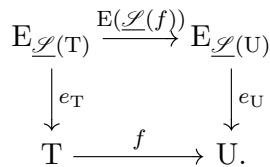
\includegraphics[keepaspectratio]{images/part001_16180f76.jpg}}
\end{enumerate}

对第一个图，这由 I, p. 54 的公式 (2) 得出；对第二个图，它是定义的直接推论。由此推出：对 B 上的每一对层 \((\mathcal{F},\mathcal{G})\) 与平展 B-空间的每一对 (T,U)，上面所考虑的映射 \(\varphi\mapsto\mathrm{E}(\varphi)\) 与 \(f\mapsto\underline{\mathcal{L}}(f)\) 都是双射。

这些结果使得我们能从关于 B 上的层的一个命题推出关于平展 B-空间的一个命题，反之亦然。

\subsection{层的直像与逆像}

设 A 与 B 为拓扑空间，\(u: A \rightarrow B\) 为连续映射。

设 \(\mathcal{F} = (\mathcal{F}(\mathrm{U}), f_{\mathrm{UV}})\) 为 A 上的一个预层。我们如下定义 B 上的一个预层 \(\mathcal{F}'\)：对 B 的每个开集 U，令 \(\mathcal{F}'(\mathrm{U}) = \mathcal{F}(u^{-1}(\mathrm{U}))\)；对 B 的每对开集 (U, V) （满足 U \(\subset\) V 者），令 \(f_{\mathrm{UV}}' = f_{u^{-1}(\mathrm{U})u^{-1}(\mathrm{V})}\)。于是 \((\mathcal{F}'(\mathrm{U}), f_{\mathrm{UV}}')\) 是 B 上的一个预层。我们把它记作 \(u_{*}(\mathcal{F})\)，并称之为预层 \(\mathcal{F}\) 在映射 u 下的直像预层。

若 \((\mathrm{U}_{i})_{i\in\mathrm{I}}\) 是 B 的一族开集，则有 \(u^{-1}(\bigcup_{i\in\mathrm{I}}\mathrm{U}_{i})=\bigcup_{i\in\mathrm{I}}u^{-1}(\mathrm{U}_{i})\) 与 \(u^{-1}(\bigcap_{i\in\mathrm{I}}\mathrm{U}_{i})=\bigcap_{i\in\mathrm{I}}u^{-1}(\mathrm{U}_{i})\) （E, II, p. 25, prop. 3 与 4）。由此立即得出：若 F 具有层的性质 \((\mathrm{F}_{1})\)（相应地 \((\mathrm{F}_{2})\)）(I, p. 43)，则 \(u_{*}(\mathcal{F})\) 亦然。因此，一个层的直像是层。

设 \(\mathcal{F}_1\) 与 \(\mathcal{F}_2\) 为 A 上的预层，\(\varphi\colon\mathcal{F}_1\to\mathcal{F}_2\) 为预层的一个态射。于是存在唯一的预层态射 \(u_*\varphi\colon u_*\mathcal{F}_1\to u_*\mathcal{F}_2\)，使得对 B 的每个开集 U，映射 \((u_*\varphi)(U)\colon(u_*\mathcal{F}_1)(U)\to(u_*\mathcal{F}_2)(U)\) 就是映射 \(\varphi(u^{-1}(U))\colon\mathcal{F}_{1}(u^{-1}(U))\to\mathcal{F}_{2}(u^{-1}(U)).\) 若 \(\mathcal{F}_{3}\) 是 A 上的预层且 \(\psi\colon\mathcal{F}_{2}\to\mathcal{F}_{3}\) 是预层的态射，则有 \(u_{*}(\psi\circ\varphi)=u_{*}(\psi)\circ u_{*}(\varphi)\)。

设 C 为拓扑空间，\(v: B \to C\) 为连续映射。若 \(\mathcal{F}\) 是 A 上的预层，则预层 \(v_{*}(u_{*}(\mathcal{F}))\) 与 \((v \circ u)_{*}(\mathcal{F})\) 相同。若 \(\varphi: \mathcal{F}_{1} \to \mathcal{F}_{2}\) 是 A 上的预层态射，则有等式 \(v_{*}(u_{*}(\varphi)) = (v \circ u)_{*}(\varphi)\)。

例 1. --- 设 B 为拓扑空间，A 为 B 的一个子空间，\(\mathcal{F} = (\mathcal{F}(U), f_{\mathrm{UV}})\) 为 A 上的一个预层。用 \(i: A \to B\) 表示典范单射。于是有 \(i_*(\mathcal{F}) = (\mathcal{F}'(U), f_{\mathrm{UV}}')\)，其中对 B 的每个开集 U 有 \(\mathcal{F}'(U) = \mathcal{F}(U \cap A)\)，而对 B 的每对开集 (U, V) （满足 \(U \subset V\) 者）有 \(f_{\mathrm{UV}}' = f_{(\mathrm{U} \cap A)(\mathrm{V} \cap A)}\)。

现在设 \(\mathcal{G}\) 为 B 上的一个预层。我们定义预层 \(\mathcal{G}\) 在 \(u\) 下的逆像，并用 \(u^{*}(\mathcal{G})\) 表示层 \(\underline{\mathcal{C}}_{\mathrm{B}}(\mathrm{A};\mathrm{E}_{\mathcal{G}})\) （A 上的、以 B-空间 \(\mathrm{E}_{\mathcal{G}}\) 为值的 B-态射所成的层）（I, p. 45, 例 4）。它典范同构于 A-平展空间 \(\mathrm{A} \times_{\mathrm{B}} \mathrm{E}_{\mathcal{G}}\) 的截面在 A 上所成的层 (I, p. 9, prop. 3)。由此我们推出 (I, p. 52, 例 2) 一个典范同构 \(\varphi\)，它把与 \(u^{*}(\mathcal{G})\) 相伴的平展空间映到 A-空间 \(\mathrm{A} \times_{\mathrm{B}} \mathrm{E}_{\mathcal{G}}\) 上。此外，若 \(\mathcal{G}\) 是层，则对 A 的每一点 \(a\) 有一个典范双射 \(\psi_{a}: u^{*}(\mathcal{G})_{a} \to \mathcal{G}_{u(a)}\)：对 \(a\) 在 A 中的每个开邻域 U 与每个 B-态射 \(f: \mathrm{U} \to \mathrm{E}_{\mathcal{G}}\)，我们有

\[
\varphi ([ \mathrm{U}, f, a ]) = (a, f (a)), \quad \psi_ {a} ([ \mathrm{U}, f, a ]) = f (a).
\]

设 \(\mathcal{G}_1\) 与 \(\mathcal{G}_2\) 为 B 上的预层，\(\varphi\colon\mathcal{G}_1\to\mathcal{G}_2\) 为预层的一个态射。由 B-平展空间的态射 \(\mathrm{E}(\varphi)\colon\mathrm{E}_{\mathcal{G}_1}\to\mathrm{E}_{\mathcal{G}_2}\) 经基变换，我们导出 A-平展空间的一个态射 \(\mathrm{A}\times_{\mathrm{B}}\mathrm{E}_{\mathcal{G}_1}\to\mathrm{A}\times_{\mathrm{B}}\mathrm{E}_{\mathcal{G}_2}\)，从而导出 A 上的层的一个态射 \(u^{*}(\varphi)\colon u^{*}(\mathcal{G}_{1})\to u^{*}(\mathcal{G}_{2})\)。设 \(\mathcal{G}_3\) 为 B 上的预层，\(\psi\colon\mathcal{G}_2\to\mathcal{G}_3\) 为预层的一个态射。于是有等式 \(u^{*}(\psi\circ\varphi)=u^{*}(\psi)\circ u^{*}(\varphi)\)。

设 C 为拓扑空间，\(v\colon B \to C\) 为连续映射。若 \(\mathcal{G}\) 是 C 上的预层，则层 \(u^{*}(v^{*}(\mathcal{G}))\) 与 \((v \circ u)^{*}(\mathcal{G})\) 典范地等同 (I, p. 5)。若 \(\varphi\colon\mathcal{G}_{1} \to \mathcal{G}_{2}\) 是 C 上的预层态射，则更有 \(u^{*}(v^{*}(\varphi)) = (v \circ u)^{*}(\varphi)\)。

注. --- I, p. 53 中的典范态射 \(\sigma_{\mathcal{G}}\colon\mathcal{G}\to\widetilde{\mathcal{G}}\) 用平展空间的语言对应于 I, p. 53 命题 2 的同构 \(j_{\mathcal{G}}\)。由此推出 \(u^{*}(\sigma_{\mathcal{G}})\) 是同构。特别地，若 \(A = B\) 且 \(u = \mathrm{Id}_A\)，则预层 \(u^{*}(\mathcal{F})\) 就是层 \(\widetilde{\mathcal{F}}\)。

例 2. --- 设 B 为拓扑空间，A 为 B 的一个子空间。用 \(i\colon\mathrm{A}\to\mathrm{B}\) 表示典范单射。对 B 上的每个层 \(\mathcal{G}\)，用 \(\mathcal{G}_{\mathrm{A}}\) 表示层 \(i^{*}(\mathcal{G})\)，并称 \(\mathcal{G}_{\mathrm{A}}\) 为由层 \(\mathcal{G}\) 在 A 上诱导的层。层 \(\mathcal{G}_{\mathrm{A}}\) 等同于层 \(\underline{\mathcal{L}}(\mathrm{A};(\mathrm{E}_{\mathcal{G}})_{\mathrm{A}})\) ，即由 \(\mathrm{E}_{\mathcal{G}}\) 在 A 上诱导的 A-平展空间的截面所成的层。

设 A 是 B 的一个开子空间，\(\mathcal{G}\) 是 B 上的一个层。按定义，层 \(\mathcal{G}_{\mathrm{A}}\) 是层 \(\widetilde{\mathcal{G}}\mid \mathrm{A}\) （由 \(\widetilde{\mathcal{G}}\) 限制到开集 A 而得者）(I, p. 43)。设 \(\sigma_{\mathcal{G}}\colon \mathcal{G}\to \widetilde{\mathcal{G}}\) 为典范同构 (I, p. 55, cor. 1)。于是 \(\sigma_{\mathcal{G}}\mid \mathrm{A}\) 是从层 \(\mathcal{G}\mid \mathrm{A}\) 到层 \(\mathcal{G}_{\mathrm{A}}\) 上的一个典范同构，称为从 \(\mathcal{G}\mid \mathrm{A}\) 到 \(\mathcal{G}_{\mathrm{A}}\) 上的典范同构。

\subsection{\texorpdfstring{同态 \(\alpha\) 与 \(\beta\)；伴随}{同态 alpha 与 beta；伴随}}

设 A 与 B 为拓扑空间，\(u\colon\mathrm{A}\to\mathrm{B}\) 为连续映射。设 \(\mathcal{G}\) 为 B 上的一个预层。由预层直像的定义，层 \(u_{*}u^{*}\mathcal{G}\) 在 B 的开集 U 上的截面是层 \(u^{*}\mathcal{G}\) 在 A 的开集 \(u^{-1}(\mathrm{U})\) 上的截面，也就是一个 B-态射 \(u^{-1}(\mathrm{U})\to\mathrm{E}_{\mathcal{G}}\)。于是，下述对应定义了一个层的态射 \(\widetilde{\mathcal{G}}\to u_{*}u^{*}\mathcal{G}\)：把截面 \(s\) （\(\mathrm{E}_{\mathcal{G}}\) 在 B 的一个开集 U 上的）对应为截面 \(s\circ u\) （\(\mathrm{E}_{\mathcal{G}}\) 在 \(u^{-1}(\mathrm{U})\) 上的）。该态射与典范态射 \(\sigma_{\mathcal{G}}\colon\mathcal{G}\to\widetilde{\mathcal{G}}\) （I, p. 53）的复合是一个预层态射 \(\mathcal{G}\to u_{*}u^{*}\mathcal{G}\)，将记作 \(\beta_{\mathcal{G}}^{u}\)，甚至记作 \(\beta_{\mathcal{G}}\) （当映射 \(u\) 无歧义时）。

注. --- 1) 设 A、B、C 为拓扑空间，\(u\colon A \to B\)、\(v\colon B \to C\) 为连续映射；令 \(w = v \circ u\)。设 \(\mathcal{G}\) 为 C 上的一个预层。

设 U 为 C 的开集，s 为 \(E_{G}\) 在 U 上的一个截面。于是 \(\beta_{\mathcal{G}}^{v}(s)\) 是截面 \(s \circ v\) （\(E_{G}\) 在 \(v^{-1}(U)\) 上的），而 \(v_{*}(\beta_{v^{*}\mathcal{G}}^{u})(\beta_{\mathcal{G}}^{v}(s))\) 是截面 \(s \circ v \circ u = s \circ w\) （\(E_{G}\) 在 \(u^{-1}(v^{-1}(U)) = w^{-1}(U)\) 上的）。

由此得 \(\beta_{\mathcal{G}}^{w} = v_{*}(\beta_{v^{*}\mathcal{G}}^{u})\circ \beta_{\mathcal{G}}^{v}\)。

\begin{enumerate}
\def\labelenumi{\arabic{enumi})}
\setcounter{enumi}{1}
\tightlist
\item
  若 \(\gamma\colon\mathcal{G}_{1}\to\mathcal{G}_{2}\) 是 B 上的预层态射，则预层态射 \(\beta_{\mathcal{G}_{2}}\circ\gamma\) 与 \(u_{*}u^{*}(\gamma)\circ\beta_{\mathcal{G}_{1}}\) 相等。事实上，若 V 是 B 的开集且 \(s\in\mathcal{G}_{1}(V)\)，则 \(\beta_{\mathcal{G}_{1}}(s)\) 是截面 \(t\) （A \(\times_{B}E_{\mathcal{G}_{1}}\) 在 \(u^{-1}(V)\) 上的），由 \(x\mapsto(x,[V,s,u(x)])\) 定义。于是 \(t\) 在 \(u^{*}(\gamma)\) 下的像是 A \(\times_{B}E_{\mathcal{G}_{2}}\) 在 \(u^{-1}(V)\) 上由 \(x\mapsto(x,[V,\gamma(s),u(x)])\) 给出的截面。由此得 \(u_{*}u^{*}(\gamma)\circ\beta_{\mathcal{G}_{1}}(s)=\beta_{\mathcal{G}_{2}}(\gamma(s))\)。
\end{enumerate}

命题 4. --- 设 A 与 B 为拓扑空间，\(u\colon A\to B\) 为连续映射，\(\mathcal{G}\) 为 B 上的一个预层，\(\mathcal{F}\) 为 A 上的一个层。

对每个预层态射 \(\varphi\colon\mathcal{G}\to u_{*}\mathcal{F}\)，存在唯一的层的态射 \(\psi\colon u^{*}(\mathcal{G})\to\mathcal{F}\) 满足 \(\varphi=u_{*}(\psi)\circ\beta_{\mathcal{G}}\)。

换言之，典范映射

\[
\operatorname{Mor} \left(u ^ {*} (\mathcal {G}), \mathcal {F}\right)\rightarrow \operatorname{Mor} \left(\mathcal {G}, u _ {*} (\mathcal {F})\right), \quad \psi \mapsto u _ {*} (\psi) \circ \beta_ {\mathcal {G}}
\]

是双射。

采用命题 4 的记号，我们有时记 \(\psi = \varphi^{\sharp}\) 与 \(\varphi = \psi^{\flat}\)。

我们来证明命题 4。把注 2 应用于态射 \(\sigma_{\mathcal{G}}: \mathcal{G} \to \widetilde{\mathcal{G}}\)，便知态射 \(\beta_{\mathcal{G}}\) 等于复合

\[
u _ {*} (u ^ {*} (\sigma_ {\mathcal {G}}) ^ {- 1}) \circ \beta_ {\widetilde {\mathcal {G}}} \circ \sigma_ {\mathcal {G}},
\]

其中 \(u^{*}(\sigma_{\mathcal{G}}) \colon u^{*}(\mathcal{G}) \to u^{*}(\widetilde{\mathcal{G}})\) 是 I, p. 58 的注中的典范同构。设 \(\widetilde{\varphi} \colon \widetilde{\mathcal{G}} \to u_{*}\mathcal{F}\) 为唯一的层的态射，满足 \(\widetilde{\varphi} \circ \sigma_{\mathcal{G}} = \varphi\) (I, p. 54, prop. 3)。于是只需证明：存在唯一的层的态射 \(\widetilde{\psi} \colon u^{*}(\mathcal{G}) \to \mathcal{F}\) 满足 \(u_{*}(\widetilde{\psi}) \circ \beta_{\widetilde{\mathcal{G}}} = \widetilde{\varphi}\)。

因此我们可以假设 \(\mathcal{G}\) 是层。为使层的态射 \(\psi: u^{*}(\mathcal{G}) \to \mathcal{F}\) 满足命题 4 的结论，必须且只需：对 B 的每个开集 V 与每个截面 \(t\) （\(\mathrm{E}_{\mathcal{G}}\) 在 V 上的），有

\[
\varphi_{\mathrm{V}}(t) = \psi_{u^{-1}(\mathrm{V})}(t \circ u \mid u^{-1}(\mathrm{V})).\tag{6}
\]

设 \(U_{0}\) 为 A 的一个开子集，\(s_{0}\) 为 \(u^{*}(\mathcal{G})(\mathrm{U}_{0})\) 的一个元素，换言之，是从 \(U_{0}\) 到 \(E_{\mathcal{G}}\) 中的一个 B-态射。设 \(\mathrm{S}(\mathrm{U}_{0}, s_{0})\) 为三元组 \((\mathrm{U}, \mathrm{V}, t)\) 所成的集，其中 U 是 A 的含于 \(U_{0}\) 的开子集，V 是 B 的满足 \(u(\mathrm{U}) \subset \mathrm{V}\) 的开子集，而 t 是 \(E_{\mathcal{G}}\) 在 V 上的一个截面，且满足

\[
t \circ u \mid \mathrm{U} = s _ {0} \mid \mathrm{U}.\tag{7}
\]

若 \(U_{1}\) 与 \(U_{2}\) 是 A 的开子集且 \(U_{1} \subset U_{2}\)，则用 \(f_{U_{1}U_{2}}\) 表示限制映射 \(\mathcal{F}(U_{2}) \to \mathcal{F}(U_{1})\)。于是对每个 \((\mathrm{U}, \mathrm{V}, t) \in \mathrm{S}(\mathrm{U}_{0}, s_{0})\)，我们有关系式

\[
\begin{array}{l} f_{\mathrm{U}\mathrm{U}_{0}}(\psi_{\mathrm{U}_{0}}(s_{0})) = \psi_{\mathrm{U}}(s_{0} \mid \mathrm{U}) \\ \qquad = \psi_{\mathrm{U}}(t \circ u \mid \mathrm{U}) \\ \qquad = f_{\mathrm{U}u^{-1}(\mathrm{V})}(\psi_{u^{-1}(\mathrm{V})}(t \circ u \mid u^{-1}(\mathrm{V}))). \end{array}
\]

因此，若 \(\psi \colon u^{*}(\mathcal{G})\to \mathcal{F}\) 满足 (6)，则我们有

\[
f_{\mathrm{U}\mathrm{U}_{0}}(\psi_{\mathrm{U}_{0}}(s_{0})) = f_{\mathrm{U}u^{-1}(\mathrm{V})}(\varphi_{\mathrm{V}}(t)).\tag{8}
\]

我们来证明：对每一点 \(a\) （属于 \(\mathrm{U}_0\) 者），存在三元组 \((\mathrm{U},\mathrm{V},t)\in \mathrm{S}(\mathrm{U}_0,s_0)\) 使得 \(a\in \mathrm{U}\)。事实上，设 \(a\) 为 \(\mathrm{U}_0\) 的一点。存在 B 中包含 \(u(a)\) 的开邻域 V，以及截面 \(t\) （平展空间 \(\mathbf{E}_{\mathcal{G}}\) 在 V 上的），使得 \(t(u(a)) = s_0(a)\) (I, p. 33, prop. 9)。令 \(\mathrm{U}_1 = u^{-1} (\mathrm{V})\cap \mathrm{U}_0\)。截面 \(s_0\mid \mathrm{U}_1\) 与 \(t\circ u\mid \mathrm{U}_1\) ——即 \(\mathrm{U}_1\) 上的平展空间 \(\mathbf{E}_{\mathcal{G}}\times_{\mathrm{B}}\mathrm{U}_1\) 的截面——在点 \(a\) 处相合。由 I, p. 34 的 prop. 11, b)，二者相合的点所成的集是 \(\mathrm{U}_1\) 的一个包含 \(a\) 的开集 U。于是三元组 \((\mathrm{U},\mathrm{V},t)\) 属于 \(\mathrm{S}(\mathrm{U}_0,s_0)\)。

于是，公式 (8) 与层的性质 \((\mathrm{F}_{1})\) (I, p. 43) 蕴涵 \(\psi\) 的唯一性。

设 (U, V, t) 与 \((\mathrm{U}^{\prime}, \mathrm{V}^{\prime}, t^{\prime})\) 为 \(\mathrm{S}(\mathrm{U}_{0}, s_{0})\) 的元素。由关系式 (7)，t 与 \(t^{\prime}\) 在 \(u(\mathrm{U} \cap \mathrm{U}^{\prime})\) 上的限制相合。由 I, p. 34 的 prop. 11, b)，存在 B 的开集 W 满足 \(u(\mathrm{U} \cap \mathrm{U}^{\prime}) \subset \mathrm{W} \subset \mathrm{V} \cap \mathrm{V}^{\prime}\) 且 \(t \mid W = t^{\prime} \mid W\)。因此我们有

\[
f_{u^{-1}(\mathrm{W})u^{-1}(\mathrm{V})}(\varphi_{\mathrm{V}}(t)) = \varphi_{\mathrm{W}}(t\mid \mathrm{W}) = \varphi_{\mathrm{W}}(t^{\prime}\mid \mathrm{W}) = f_{u^{-1}(\mathrm{W})u^{-1}(\mathrm{V}^{\prime})}(\varphi_{\mathrm{V}^{\prime}}(t^{\prime}))
\]

从而

\[
f_{(\mathrm{U}\cap\mathrm{U}^{\prime})u^{-1}(\mathrm{V})}(\varphi_{\mathrm{V}}(t)) = f_{(\mathrm{U}\cap\mathrm{U}^{\prime})u^{-1}(\mathrm{V}^{\prime})}(\varphi_{\mathrm{V}^{\prime}}(t^{\prime})).\tag{9}
\]

由层 F 的性质 \((\mathrm{F}_{1})\) 与 \((\mathrm{F}_{2})\)，存在唯一的元素 \(s'\) （\(\mathcal{F}(\mathrm{U}_{0})\) 的），使得对每个三元组 \((\mathrm{U},\mathrm{V},t)\) （取自

\(\mathrm{S}(\mathrm{U}_{0},s_{0})\) 者），有：

\[
f_{\mathrm{U}\mathrm{U}_{0}}(s^{\prime}) = f_{\mathrm{U}u^{-1}(\mathrm{V})}(\varphi_{\mathrm{V}}(t)).\tag{10}
\]

把这个元素记作 \(\psi_{\mathrm{U}_{0}}(s_{0})\)。

设 \(U_{1}\) 为含于 \(U_{0}\) 的开集，且 \(s_{1}=s_{0}|U_{1}\)。若 \((\mathrm{U},\mathrm{V},t)\in\mathrm{S}(\mathrm{U}_{1},s_{1})\)，则 U 是含于 \(U_{0}\) 的开集且 \(t\circ u|U=s_{1}|U=s_{0}|U\)，因此 \((\mathrm{U},\mathrm{V},t)\in\mathrm{S}(\mathrm{U}_{0},s_{0})\)，而关系式 (10) 这时蕴涵

\[
f_{\mathrm{U}\mathrm{U}_{1}}(f_{\mathrm{U}_{1}\mathrm{U}_{0}}(\psi_{\mathrm{U}_{0}}(s_{0}))) = f_{\mathrm{U}\mathrm{U}_{0}}(\psi_{\mathrm{U}_{0}}(s_{0})) = f_{\mathrm{U}u^{-1}(\mathrm{V})}(\varphi_{\mathrm{V}}(t)).
\]

由 \(\psi_{\mathrm{U}_{1}}(s_{1})\) 的定义，我们于是有 \(\psi_{\mathrm{U}_{1}}(s_{1}) = f_{\mathrm{U}_{1}\mathrm{U}_{0}}(\psi_{\mathrm{U}_{0}}(s_{0}))\)。这就证明了族 \(\psi = (\psi_{\mathrm{U}})\) 是从 \(u^{*}(\mathcal{G})\) 到 \(\mathcal{F}\) 中的层的态射。

我们来证明 \(\psi\) 满足关系式 (6)。设 V 为 B 的开子集，\(t\) 为 \(\mathrm{E}_{\mathcal{G}}\) 在 V 上的一个截面。若 \(\mathrm{U} = u^{-1}(\mathrm{V})\) 且 \(s = t \circ u \mid \mathrm{U}\)，则三元组 \((\mathrm{U}, \mathrm{V}, t)\) 属于 \(\mathrm{S}(\mathrm{U}, s)\)，而关系式 (6) 是关系式 (10) （应用到 \(\mathrm{U} = \mathrm{U}_0\)）的直接推论。

命题 5. — 设 A 与 B 为拓扑空间，u: A → B 为连续映射。

\begin{enumerate}
\def\labelenumi{\alph{enumi})}
\tightlist
\item
  设 \(\mathcal{G}_1\) 与 \(\mathcal{G}_2\) 为 B 上的预层，\(\gamma\colon\mathcal{G}_1\to\mathcal{G}_2\) 为预层的一个态射。再设 \(\mathcal{F}\) 为 A 上的层，\(\varphi\colon\mathcal{G}_2\to u_*\mathcal{F}\) 为预层的一个态射。我们有等式
\end{enumerate}

\[
(\varphi \circ \gamma) ^ {\sharp} = \varphi^ {\sharp} \circ u ^ {*} (\gamma).\tag{11}
\]

\begin{enumerate}
\def\labelenumi{\alph{enumi})}
\setcounter{enumi}{1}
\tightlist
\item
  设 \(\mathcal{F}_1\) 与 \(\mathcal{F}_2\) 为 A 上的层，\(\mathcal{G}\) 为 B 上的一个预层。设 \(\varphi\colon\mathcal{F}_1\to\mathcal{F}_2\) 为层的一个态射，\(\gamma\colon\mathcal{G}\to u_*\mathcal{F}_1\) 为预层的一个态射。我们有关系式
\end{enumerate}

\[
(u _ {*} (\varphi) \circ \gamma) ^ {\sharp} = \varphi \circ \gamma^ {\sharp}.
\]

\begin{enumerate}
\def\labelenumi{\alph{enumi})}
\tightlist
\item
  由 \(\varphi^{\sharp}\) 的定义与 I, p. 60 的注 2，我们有
\end{enumerate}

\[
\varphi \circ \gamma = u _ {*} (\varphi^ {\sharp}) \circ \beta_ {\mathcal {G} _ {2}} \circ \gamma = u _ {*} (\varphi^ {\sharp}) \circ u _ {*} u ^ {*} (\gamma) \circ \beta_ {\mathcal {G} _ {1}}.
\]

因此，\(\varphi \circ \gamma = u_{*}(\varphi^{\sharp}\circ u^{*}(\gamma))\circ \beta_{\mathcal{G}_{1}}\)；由此得关系式 (11)。

\begin{enumerate}
\def\labelenumi{\alph{enumi})}
\setcounter{enumi}{1}
\tightlist
\item
  由 \(\gamma^{\sharp}\) 的定义，我们有
\end{enumerate}

\[
u _ {*} (\varphi) \circ \gamma = u _ {*} (\varphi) \circ u _ {*} (\gamma^ {\sharp}) \circ \beta_ {\mathcal {G}} = u _ {*} (\varphi \circ \gamma^ {\sharp}) \circ \beta_ {\mathcal {G}},
\]

从而得到所宣布的关系式，这里用到了 \((u_{*}(\varphi)\circ\gamma)^{\sharp}\) 的定义。

令 \(\alpha_{\mathcal{F}} = \mathrm{Id}_{u_*(\mathcal{F})}^\sharp\)；它是唯一的层的态射 \(\rho \colon u^*(u_*(\mathcal{F})) \to \mathcal{F}\)，满足

\[
\operatorname{Id} _ {u _ {*} (\mathcal {F})} = u _ {*} (\rho) \circ \beta_ {u _ {*} (\mathcal {F})}.
\]

把关系式 (11) 应用于 \(\mathcal{G}_2 = u_*(\mathcal{F})\) 与态射 \(\varphi = \mathrm{Id}_{u_*(\mathcal{F})}\)，就对每个预层态射 \(\gamma\colon\mathcal{G}\to u_*(\mathcal{F})\) 给出分解式

\[
\gamma^ {\sharp} = \alpha_ {\mathcal {F}} \circ u ^ {*} (\gamma).
\]

于是由命题 4 推出：对每个层的态射 \(\psi\) （从 \(u^{*}(\mathcal{G})\) 到 \(\mathcal{F}\) 中的），\(\psi^{\flat}\) 是唯一的态射 \(\varphi\colon\mathcal{G}\to u_{*}(\mathcal{F})\) 满足 \(\psi=\alpha_{\mathcal{F}}\circ u^{*}(\varphi)\)。

例. --- 1) 考察拓扑空间 B、B 的子空间 A，并用 \(i\colon A \to B\) 表示典范单射。设 \((E,p)\) 与 \((E',p')\) 为 B-空间。取 \(\mathcal{G}\) 为层 \(\underline{\mathcal{M}or}_{B}(E;E')\) （I, p. 45, 例 4），取 \(\mathcal{F}\) 为层 \(\underline{\mathcal{M}or}_{A}(E_{A};E_{A}')\)。对 B 的每个开集 V 与每个 V-态射 \(f\colon E_{V} \to E_{V}'\)，令 \(\varphi_{V}(f) = f_{V \cap A}\)，其中 \(f_{V \cap A}\) 是 \((V \cap A)\) -态射 （从 \(E_{V \cap A}\) 到 \(E_{V \cap A}'\) 中的、由 \(f\) 诱导者）。如此定义的族 \(\varphi = (\varphi_{V})\) 是从 \(\mathcal{G}\) 到 \(i_*\mathcal{F}\) 中的层的态射。由命题 4，存在唯一的层的态射 \(\psi\colon \underline{\mathcal{M}or}_{B}(E;E')_{A} \to \underline{\mathcal{M}or}_{A}(E_{A};E_{A}')\)，使得有

\[
\psi_ {\mathrm{V} \cap \mathrm{A}} (\sigma_ {\mathcal {G}} (\mathrm{V}, f) \mid \mathrm{V} \cap \mathrm{A}) = f _ {\mathrm{V} \cap \mathrm{A}}\tag{12}
\]

对 B 的每个开集 V 与每个 \(f \in \mathcal{C}_{\mathrm{V}}(\mathrm{E}_{\mathrm{V}}; \mathrm{E}_{\mathrm{V}}^{\prime})\) 成立。态射 \(\psi\) 称为从 \(\underline{\mathcal{M}or_{B}}(\mathrm{E}; \mathrm{E}^{\prime})_{\mathrm{A}}\) 到 \(\underline{\mathcal{M}or_{A}}(\mathrm{E}_{\mathrm{A}}; \mathrm{E}_{\mathrm{A}}^{\prime})\) 中的典范态射。

若 A 缩为一个单点 \(a\)，则该态射等同于从 \(a\) 处的茎（层 \(\underline{\mathcal{M}or}_{\mathrm{B}}(\mathrm{E};\mathrm{E}^{\prime})\) 的）到集合 \(\mathcal{C}(\mathrm{E}_a;\mathrm{E}_a')\) 中的态射。

通过过渡到子层，态射 \(\psi\) 诱导出从 \(\mathcal{I}som_{\mathrm{B}}(\mathrm{E};\mathrm{E}')_{\mathrm{A}}\) 到 \(\mathcal{I}som_{\mathrm{A}}(\mathrm{E}_{\mathrm{A}};\mathrm{E}_{\mathrm{A}}^{\prime})\) 中的一个典范态射。

\begin{enumerate}
\def\labelenumi{\arabic{enumi})}
\setcounter{enumi}{1}
\tightlist
\item
  设 A、B、C 为拓扑空间，\(u\colon A\to B\)、\(v\colon B\to C\) 为连续映射；令 \(w=v\circ u\)。设 E 与 E' 为 C-空间。从 \(\underline{\mathcal{M}or}_{C}(E;E')_{A}\) 到 \(\underline{\mathcal{M}or}_{A}(E_{A};E'_{A})\) 中的典范态射是这样一个态射与另一个典范态射的复合：前者为 \(\underline{\mathcal{M}or}_{C}(E;E')_{A}\to\underline{\mathcal{M}or}_{B}(E_{B};E'_{B})_{A}\) （由 \(\underline{\mathcal{M}or}_{C}(E;E')_{B}\) 到 \(\underline{\mathcal{M}or}_{B}(E_{B};E'_{B})\) 中的典范态射导出者），后者为从 \(\underline{\mathcal{M}or}_{B}(E_{B},E'_{B})_{A}\) 到 \(\underline{\mathcal{M}or}_{A}(E_{A},E'_{A})\) 中的典范态射。
\end{enumerate}

\subsection{柔软层}

定义 5. --- 设 \(p\colon E \rightarrow B\) 为平展映射。称映射 \(p\) 是柔软的，或称平展 B-空间 \((E,p)\) 是柔软的，如果 \(p\) 在 B 的闭子空间上的每个连续截面都能扩张为 \(p\) 在 B 上的一个连续截面。

设 F 为 B 上的一个层。若相伴的平展空间 (I, p. 50, def. 4) 是柔软的，则称 F 为柔软层。

设 \(\mathcal{F}\) 为 B 上的层。层 \(\mathcal{F}\) 是柔软的，当且仅当：对 B 的每个闭集 Z、Z 的每个开邻域 U 以及每个 \(s \in \mathcal{F}(\mathrm{U})\) ，存在 \(t \in \mathcal{F}(\mathrm{B})\) 以及 Z 的一个含于 U 的开邻域 V，使得 \(s \mid \mathrm{V} = t \mid \mathrm{V}\) 。

若 \(\mathcal{F}\) 是柔软层，则 \(\mathcal{F}(\mathrm{B})\) 非空：事实上，平展空间 \(\mathrm{E}_{\mathcal{F}}\) （与层 \(\mathcal{F}\) 相伴者）在 \(\varnothing\) 上的唯一截面可扩张为 \(\mathrm{E}_{\mathcal{F}}\) 在 B 上的连续截面。

设 \(p \colon \mathrm{E} \to \mathrm{B}\) 为平展映射，并设 A 为 B 的闭子空间。若 \(p\) 是柔软的，则映射 \(p_{\mathrm{A}} \colon \overline{p}^{1}(\mathrm{A}) \to \mathrm{A}\) 是柔软的。等价地，若 \(\mathcal{F}\) 是 B 上的柔软层，则它在闭子空间 A 上诱导的层是柔软的。

命题 6. --- 设 B 为拓扑空间，\(\mathcal{F}\) 为 B 上的层，\((\mathrm{A}_i)_{i\in \mathrm{I}}\) 为 B 的局部有限闭覆盖。层 \(\mathcal{F}\) 是柔软的，当且仅当对每个 \(i\in \mathrm{I}\)，诱导层 \(\mathcal{F}_{\mathrm{A}_i}\) 都是柔软的。

该条件显然是必要的。我们来证明它是充分的。用 \(p\colon \mathrm{E}\to \mathrm{B}\) 表示 B-平展空间 \(\mathrm{E}_{\mathcal{F}}\) （与层 \(\mathcal{F}\) 相伴者）。设 A 为 B 的闭子空间，并设 \(s\colon \mathrm{A}\to \mathrm{E}\) 为 \(p\) 在 A 上的一个连续截面；须证 \(s\) 具有到 B 上的连续扩张。对 I 的每个子集 J，令 \(\mathrm{A_J} = \bigcup_{i\in \mathrm{J}}\mathrm{A}_i\) ；集 \(\mathrm{A_J}\) 在 B 中是闭的 (TG, I, p. 6, prop. 4)。

设 \(\mathcal{S}\) 为由数对 \((\mathrm{J},t)\) 组成的集，其中 \(\mathrm{J}\) 是 I 的子集，而 \(t\) 是 E 在 \(\mathrm{A_J}\) 上的连续截面，且与 \(s\) 在 \(\mathrm{A} \cap \mathrm{A_J}\) 上重合。给 \(\mathcal{S}\) 赋以记作 \(\leqslant\) 的序关系：\((\mathrm{J},t) \leqslant (\mathrm{J}',t')\) 如果 \(\mathrm{J} \subset \mathrm{J}'\) 且 \(t' \mid \mathrm{A_J} = t\) 。对 \(\sigma = (\mathrm{J},t) \in \mathcal{S}\) ，记 \(\mathrm{J}_{\sigma} = \mathrm{J}\) 与 \(t_{\sigma} = t\) 。我们来证明序集 \(\mathcal{S}\) 是归纳的。设 S 为 \(\mathcal{S}\) 的一个全序子集。令 \(\mathrm{J} = \bigcup_{\sigma \in \mathrm{S}} \mathrm{J}_{\sigma}\) ；它是 I 的一个子集。于是便定义了截面 \(t\) （E 在 \(\mathrm{A_J}\) 上的），令 \(t(x) = t_{\sigma}(x)\) （当 \(x \in \mathrm{A}_{J_{\sigma}}\) 时）；因而有 \(t \mid \mathrm{A} \cap \mathrm{A_J} = s\) 。设 \(j \in \mathrm{J}\)，并设 \(\sigma \in S\) 使 \(j \in J_{\sigma}\) ；由于 \(t \mid A_j = t_{\sigma} \mid A_j\) ，\(t\) 在 \(A_j\) 上的限制是连续的。于是由 TG, I, p. 19, prop. 4 知 \(t\) 是连续的。这样，(J, t) 便是 \(\mathcal{S}\) 的元素；按构造，它是 S 的一个上界。这就证明了集 \(\mathcal{S}\) 是归纳的。因此它具有一个极大元 (J, t) (E, III, p. 20, th. 2)。

我们用反证法，假设 \(J \neq I\) 。设 i 为 \(I \setminus J\) 的一个元素。令 \(A' = (A_i \cap A) \cup (A_i \cap A_J)\)，并定义截面 \(s'\) （E 在 \(A'\) 上的）如下：

\[
s ^ {\prime} (a) = \left\{ \begin{array}{l l} s (a) & \text {for} a \in \mathrm{A} _ {i} \cap \mathrm{A}, \\ t (a) & \text {for} a \in \mathrm{A} _ {i} \cap \mathrm{A} _ {\mathrm{J}}, \end{array} \right.
\]

这是可能的，因为 \(s\) 与 \(t\) 在 \(\mathrm{A} \cap \mathrm{A}_{\mathrm{J}}\) 上重合。此外，由于 \(\mathrm{A}_{i} \cap \mathrm{A}\) 与 \(\mathrm{A}_{i} \cap \mathrm{A}_{\mathrm{J}}\) 都是闭集，截面 \(s'\) 是连续的 (TG, I, p. 19, prop. 4)。按假设，存在连续截面 \(s_{i}: \mathrm{A}_{i} \to \mathrm{E}\) 使之扩张 \(s'\) 。由于 \(s_{i}\) 与 \(t\) 在 \(\mathrm{A}_{\mathrm{J}} \cap \mathrm{A}_{i}\) 上的限制相等，映射 \(t': \mathrm{A}_{\mathrm{J} \cup \{i\}} \to \mathrm{E}\) （与 \(t\) 在 \(\mathrm{A}_{\mathrm{J}}\) 上重合、与 \(s_{i}\) 在 \(\mathrm{A}_{i}\) 上重合者）便是 \(p\) 在 \(\mathrm{A}_{\mathrm{J} \cup \{i\}}\) 上的连续截面，且它扩张 \(s| \mathrm{A} \cap \mathrm{A}_{\mathrm{J} \cup \{i\}}\) 。于是有 \((\mathrm{J}, t) < (\mathrm{J} \cup \{i\}, t')\) ，这与 \((\mathrm{J}, t)\) 为极大元的假设相矛盾。

于是 J = I，从而 \(A_{J} = B\)，且 t 是 E 在 B 上的连续截面，它扩张 s。

推论 1. --- 设 B 为仿紧空间，\(\mathcal{F}\) 为 B 上的层，\((\mathrm{U}_i)_{i\in \mathrm{I}}\) 为 B 的开覆盖。若对每个 \(i\in \mathrm{I}\) ，诱导层 \(\mathcal{F}|\mathrm{U}_i\) 都是柔软的，则层 \(\mathcal{F}\) 是柔软的。

事实上，存在局部有限闭覆盖 \((\mathrm{F}_{j})_{j\in\mathrm{J}}\) ，它比覆盖 \((\mathrm{U}_{i})_{i\in\mathrm{I}}\) 更细 (TG, IX, p. 49, prop. 4 及 p. 48, cor. 1)。于是，对每个 \(j\in J\)，层 \(\mathcal{F}|F_{j}\) 是柔软的，而命题蕴含层 \(\mathcal{F}\) 是柔软的。

推论 2. --- 设 B 为仿紧空间，\(\mathcal{F}\) 为 B 上的层，\((\mathrm{A}_i)_{i\in \mathrm{I}}\) 为 B 的局部有限闭覆盖。为使层 \(\mathcal{F}\) 是柔软的，必须且只需下述条件成立：

对每个 \(i \in I\) 、\(A_{i}\) 的每个闭子集 A、B 的每个含 A 的开集 V 以及 \(\mathcal{F}(V)\) 的每个元素 s，存在 \(A_{i}\) 在 B 中的一个开邻域 U、\(\mathcal{F}(U)\) 的一个元素 t 以及 A 在 B 中的一个含于 \(U \cap V\) 的开邻域 W，使得 \(t | W = s | W\) 。

设层 \(\mathcal{F}\) 是柔软的，我们来证明该条件成立。设 \(i\in\mathrm{I}\) ，设 A 为 \(\mathrm{A}_{i}\) 的闭子集，设 V 为 B 的含 A 的开集，并设 \(s\) 为 \(\mathcal{F}(\mathrm{V})\) 的元素。令 \(s_{0}=\sigma_{\mathcal{F}}(s)\) 。它是平展空间 \(\mathrm{E}_{\mathcal{F}}\) 在 V 上的连续截面。由于 \(\mathrm{A}_{i}\) 是闭的，A 在 B 中是闭的，故由柔软层的定义，\(s_{0}\mid\mathrm{A}\) 可扩张为一个截面 \(t_{0}\colon\mathrm{B}\to\mathrm{E}_{\mathcal{F}}\) 。截面 \(s_{0}\) 与 \(t_{0}\mid\mathrm{V}\) （V-平展空间 \(\mathrm{E}_{\mathcal{F}}\times_{\mathrm{B}}\mathrm{V}\) 的）在 A 上重合，从而在 A 的一个邻域 W 上重合 (I, p. 34, prop. 11, b))。

反之，设推论的条件成立。由命题 6，只需证明对每个 \(i \in I\)，层 \(\mathcal{F}_{A_i}\) 是柔软的。设 A 为 \(A_i\) 的闭子集，并设 \(s_0\) 为 \(\mathcal{F} | A_i\) 的平展空间在 A 上的截面，即平展空间 \(E_{\mathcal{F}}\) 在 A 上的连续截面。由于 A 在 B 中是闭的且 B 是仿紧的，\(s_0\) 可扩张为在 B 中 A 的一个邻域 V 上的截面 \(s\) (I, p. 37, th. 2)。按假设，存在 \(A_i\) 在 B 中的一个开邻域 U 以及一个截面 \(t\) （\(E_{\mathcal{F}}\) 在 U 上的），它在 A 的一个邻域上与 \(s\) 重合。\(t\) 在 \(A_i\) 上的限制是 \(\mathcal{F}_{A_i}\) 的一个截面，且它扩张 \(s_0\) 。于是层 \(\mathcal{F}_{A_i}\) 是柔软的。由命题 6，层 \(\mathcal{F}\) 是柔软的。

\subsection{结构值层}

设给定了结构种 \(\Sigma\) 以及关于该结构种的 \(\sigma\)-态射概念。

设 B 为拓扑空间。

B 上的预层 \(\mathcal{F}\) 称为以结构种 \(\Sigma\) 为值的，如果对 B 的每个开集 U，集合 \(\mathcal{F}(\mathrm{U})\) 都赋有 \(\Sigma\) 种的结构，且诸限制映射都是 \(\sigma\)-态射。

我们将称这样的预层为以结构种 \(\Sigma\) 为值的层，如果此外它还是一个集合层。

若 \(\mathcal{F}\) 与 \(\mathcal{G}\) 都是以结构种 \(\Sigma\) 为值的预层，则称态射 \(\varphi\) 为以 \(\Sigma\) 为值的预层态射，如果对每个开集 U，映射 \(\varphi(\mathrm{U})\) 都是 \(\sigma\)-态射。

于是，例如我们可以谈论群层、交换群层、\(k\)-模层（对固定的环 \(k\)）、环层以及 \(k\)-代数层（对固定的交换环 \(k\)）。

B 上的以群（相应地，交换群、\(k\)-模、环、\(k\)-代数）为值的映射层自然地赋有群层（相应地，交换群层、\(k\)-模层、环层、\(k\)-代数层）的结构。若 X 是 R 上的 \(C^{r}\) 类微分流形，则数值函数层 \(\underline{\mathcal{C}}^{r}(\mathrm{X};\mathbf{R})\) （\(C^{r}\) 类的）是一个 R-代数层，而 X 上的向量丛 E 的 \(C^{r}\) 类截面的层是一个 R-向量空间层；微分算子定义 R-向量空间层的一个态射。

对这些结构种 \(\Sigma\)，由我们所给出的构造可知，层 \(\widetilde{\mathcal{F}}\) ——与预层 \(\mathcal{F}\) （以结构种 \(\Sigma\) 为值的，即群的、交换群的、\(k\)-模的、环的、\(k\)-代数的）相伴者—— 是以这类结构为值的层，且典范态射 \(j_{\mathcal{F}}: \mathcal{F} \to \widetilde{\mathcal{F}}\) 是以结构种 \(\Sigma\) 为值的预层态射。

例如，B 上以群为值的映射层自然地赋有群层结构。

设 A、B 为拓扑空间，并设 \(u\colon\mathrm{A}\to\mathrm{B}\) 为连续映射。若 \(\mathcal{F}\) 是 A 上以结构种 \(\Sigma\) 为值的（预）层，则（预）层 \(u_{*}(\mathcal{F})\) ——（预）层 \(\mathcal{F}\) 在 \(u\) 下的直像—— 亦然。

进一步假设结构种 \(\Sigma\) 是群、交换群、\(k\)-模、环或 \(k\)-代数的结构种。若 \(\mathcal{G}\) 是 B 上以结构种 \(\Sigma\) 为值的（预）层，则 A 上的层 \(u^{*}\mathcal{G}\) ——预层 \(\mathcal{G}\) 沿映射 \(u\) 的逆像—— 赋有一个以 \(\Sigma\) 为值的层结构。这时，伴随态射 \(\alpha\) 与 \(\beta\) 是以结构种 \(\Sigma\) 为值的预层态射。特别地，若 \(\varphi: \mathcal{G} \to u_{*}\mathcal{F}\) 是以 \(\Sigma\) 为值的预层态射，则态射 \(\varphi^{\sharp}\) 亦然；若 \(\psi: u^{*}(\mathcal{G}) \to \mathcal{F}\) 是以 \(\Sigma\) 为值的预层态射，则态射 \(\psi^{\flat}\) 亦然。

\section{覆叠}

\subsection{局部平凡纤维空间}

设 B 为拓扑空间。若 F 是拓扑空间，我们称 B-空间 \((B \times F, pr_{1})\) 为以 F 为纤维型的平凡 B-纤维空间。

设 E 为 B-空间。若存在拓扑空间 F 以及 B-同构 \(u: E \rightarrow B \times F\)，则称 B-空间 E 为可平凡化的 B-纤维空间，并称 u 为它的一个以 F 为纤维型的平凡化。

定义 1. --- 设 B 为拓扑空间。设 E 为 B-空间，p 为其投影。若 B 的每一点都有邻域 V 使 \((\overline{p}^{1}(V), p_{V})\) 是可平凡化的 V-纤维空间，则称 E 为局部平凡 B-纤维空间。

除了说“局部平凡 B-纤维空间”之外，也可说“以 B 为基的局部平凡纤维空间”。若 E 是局部平凡 B-纤维空间，有时也说 \((E,B,p)\) 是一个局部平凡纤维化，或者，滥用语言，说 p 是一个局部平凡纤维化。也称 B-空间 \((E,p)\) 在 B 的子集 A 上是可平凡化的，如果 A-空间 \(E_{A}\) （由 \((E,p)\) 在 A 上诱导者）是可平凡化的纤维空间。

设 E 为局部平凡 B-纤维空间，用 p 表示其投影。使纤维 \(\overline{p}^{1}(a)\) 为空（相应地，非空）的 B 中的点 a 所成的集是开的。于是 p 的像是 B 中既开又闭的子集。

设 F 为拓扑空间。若 E 的所有纤维都同胚于 F，则称 E 为以 F 为纤维型的局部平凡 B-纤维空间。

注. --- 1) 设 (E, p) 是 B 上的局部平凡纤维丛，并设 A 是 B 的子集。由 E 通过过渡到子空间而得的 A-空间 \(\mathrm{E}_{\mathrm{A}} = (\stackrel{-1}{p}(\mathrm{A}), p_{\mathrm{A}})\) 是局部平凡纤维空间。若 E 是可平凡化的，则 \(E_{A}\) 亦然。

事实上，对 A 的每一点 \(a\)，存在 \(a\) 在 B 中的一个开邻域 U、一个拓扑空间 F 以及一个 U-同构 \(g\colon \overline{p}^{1}(\mathrm{U})\to \mathrm{U}\times \mathrm{F}\) 。映射 \(g\) 诱导出一个 \((\mathrm{A}\cap \mathrm{U})\) -同构，它把 \(\overline{p}_{\mathrm{A}}^{-1}(\mathrm{A}\cap \mathrm{U})\)

映到 \((\mathrm{A}\cap\mathrm{U})\times\mathrm{F}\) 上，这就证明了 \(E_{A}\) 是局部平凡 A-纤维空间。

\begin{enumerate}
\def\labelenumi{\arabic{enumi})}
\setcounter{enumi}{1}
\tightlist
\item
  设 \((\mathrm{E}, p)\) 为 B-空间，并设 \((\mathrm{E}_{i})_{i \in \mathrm{I}}\) 为由开集组成的 E 的一个分划。
\end{enumerate}

若 B-空间 \((\mathrm{E}_{i}, p \mid \mathrm{E}_{i})\) 中的每一个都是可平凡化的纤维空间，则 E 是可平凡化的 B-纤维空间。事实上，对每个 \(i \in I\)，设 \(F_{i}\) 为使 B-空间 \((\mathrm{E}_{i}, p \mid \mathrm{E}_{i})\) 与 \((\mathrm{B} \times \mathrm{F}_{i}, \mathrm{pr}_{1})\) 同构的拓扑空间。于是 B-空间 \((\mathrm{E}, p)\) 同构于 \((\mathrm{B} \times \mathrm{F}, \mathrm{pr}_{1})\)，其中 F 是族 \((\mathrm{F}_{i})_{i \in I}\) 的拓扑和空间。

设集 I 是有限的。若 B-空间 \((\mathrm{E}_{i}, p \mid \mathrm{E}_{i})\) 中的每一个都是局部平凡 B-纤维空间，则 B-空间 E 亦然。事实上，由于集 I 是有限的，B 的每一点都有邻域 U，使得诸 B-纤维空间 \(E_{i}\) 在 U 上都是可平凡化的。由前所证，U-空间 \((\bar{p}^{1}(\mathrm{U}), p_{\mathrm{U}})\) 于是是可平凡化的纤维丛。

\subsection{覆叠}

定义 2. --- 覆叠是指所有纤维都是离散的局部平凡纤维空间。

除了说 B-空间 E 是一个覆叠外，也可说 E 是 B 的一个覆叠。

设 E 为 B-空间，用 p 表示其投影；设 A 为 B 的子集。若 E 是 B 的覆叠，则 p 的诸纤维是离散的，因而 \(p_{\mathrm{A}} \colon \overline{p}^{1}(\mathrm{A}) \to \mathrm{A}\) 的诸纤维也是离散的，且局部平凡 A-纤维空间 ( \(\overline{p}^{1}(\mathrm{A}), p_{\mathrm{A}}\) ) 是一个覆叠。

命题 1. --- 设 B、E 为拓扑空间，\(p\colon \mathrm{E}\to \mathrm{B}\) 为映射。下列条件等价：

\begin{enumerate}
\def\labelenumi{(\roman{enumi})}
\item
  映射 p 是连续的，且 B-空间 (E,p) 是可平凡化的覆叠。
\item
  存在由开集组成的 E 的分划 \((\mathrm{V}_{i})_{i\in\mathrm{I}}\)，使得对每个 \(i\in I\)，映射 \(p\mid V_{i}\colon V_{i}\to B\) 是同胚。
\end{enumerate}

设条件 (i) 成立，并设 \(g \colon \mathrm{E} \to \mathrm{B} \times \mathrm{F}\) 为 B-空间 \((\mathrm{E}, p)\) 的一个以 F 为纤维型的平凡化。于是，F 是离散拓扑空间，而诸集合 \(\mathrm{V}_i = g^{-1}(\mathrm{B} \times \{i\})\) （对 \(i \in F\)）构成 E 的一个由开集组成的分划。对每个 \(i\)，映射 \(p \mid V_i \colon V_i \to B\) 是同胚，其逆同胚是映射 \(x \mapsto g^{-1}(x, i)\)，由此得条件 (ii)。

反之，设条件 (ii) 成立。于是映射 p 是连续的。考虑 E 到 \(B \times I\) 中的、把 \(x \in E\) 映为偶对 \((p(x), i)\) 的映射，其中 i 是使 \(x \in V_i\) 的 I 的唯一元素。若给 I 赋以离散拓扑，则条件 (ii) 意味着此映射是 B-同构，且 B-空间 \((E, p)\) 是可平凡化的覆叠。

推论 1. --- 设 B、E 为拓扑空间，\(p\colon \mathrm{E}\to \mathrm{B}\) 为映射。为使赋有映射 \(p\) 的 E 是 B 的覆叠，必须且只需：对 B 的每一点 \(a\)，存在 \(a\) 的一个开邻域 U 以及分划 \((\mathrm{V}_i)_{i\in \mathrm{I}}\) （由 \(\overline{p}^{1}(\mathrm{U})\) 的、E 的开集组成者），使得对每个 \(i\in \mathrm{I}\)，映射 \(p\) 诱导出 \(\mathrm{V}_i\) 到 U 上的一个同胚。

注. --- 设 B 为拓扑空间。设 E 为 B-空间，p 为其投影。若 E 是 B 的覆叠，则由上述推论 1 可知，映射 p 是平展的 (I, p. 28, def. 2) 且是分离的 (I, p. 25, prop. 1, (iii))。然而，这些条件并不足以保证 E 是覆叠。例如，考虑 B 的一个开集 U。典范单射 i: U → B 是平展且分离的。为使 B-空间 (U, i) 是覆叠，必须且只需开集 U 同时是闭的。

推论 2. --- 设 B 为拓扑空间，E 为 B-空间，p 为其投影。假设 p 是平展且分离的，且空间 B 是连通的。为使 E 是 B 的可平凡化覆叠，必须且只需：对 E 的每一点 x，存在 p 的一个连续截面 s: B → E 使得 \(s(p(x)) = x\)。

这显然是必要的。反之，对任一连续截面 \(s\) （\(p\) 的），集合 \(s(\mathrm{B})\) 是开的，且映射 \(p\) 诱导出 \(s(\mathrm{B})\) 到 B 上的一个同胚 (I, p. 30, cor. 3 of prop. 6)。此外，当 \(s\) 取遍截面的集合 \(\mathcal{S}(\mathrm{B};\mathrm{E})\) （\(p\) 的）时，诸集合 \(s(\mathrm{B})\) 两两不相交，因为 B 是连通的 (I, p. 34, cor. 1 of prop. 11)。于是由命题 1 可知，若诸集合 \(s(\mathrm{B})\) 覆盖 E，则空间 E 是 B 的可平凡化覆叠。

\subsection{积与纤维积}

命题 2. --- 设 B 与 B' 为拓扑空间，(E, p) 为 B-空间，(E', p') 为 B'-空间。假设 E 与 E' 是局部平凡纤维空间（相应地，覆叠）。则空间 E × E' 赋有映射 p × p': E × E' → B × B' 后，是以 B × B' 为基的局部平凡纤维空间（相应地，覆叠）。若 E 与 E' 是可平凡化的，则 E × E' 亦然。

首先假设 B-空间 E 与 B'-空间 E' 分别有平凡化 \(g: E \to B \times F\) 与 \(g': E' \to B' \times F'\)。把同胚 \(g \times g'\) （从 \(E \times E'\) 到 \((B \times F) \times (B' \times F')\) 上的）与从 \((B \times F) \times (B' \times F')\) 到 \((B \times B') \times (F \times F')\) 上的典范同胚复合，便得到 \(B \times B'\)-空间 \(E \times E'\) 的一个以 \(F \times F'\) 为纤维型的平凡化。若 F 与 \(F'\) 是离散空间，则空间 \(F \times F'\) 也是离散的。

在一般情形，对任一点 \((a, a')\) （\(B \times B'\) 的），存在 a 在 B 中的邻域 U 与邻域 \(U'\) （\(a'\) 在 B' 中的），使得 U-空间 \(E_{U}\) 与 \(U'\)-空间 \(E_{U'}\) 都是可平凡化的。由前所证，\(B \times B'\)-空间 \(E \times E'\) 在 \(U \times U'\) 上是可平凡化的。因而它是以 \(B \times B'\) 为基的局部平凡纤维空间。若 E 与 \(E'\) 是覆叠，则其诸纤维是离散的，由此即得命题。

注意，若 \((p_{i} \colon \mathrm{E}_{i} \to \mathrm{B}_{i})_{i \in \mathrm{I}}\) 是局部平凡纤维空间的一族，甚至是覆叠的一族，则积空间 \(\prod_{i \in I} E_{i}\) 赋以映射 \((p_{i})_{i \in I}\) 后，不一定是以 \(\prod_{i \in I} B_{i}\) 为基的局部平凡纤维空间 (I, p. 145, exerc. 3)。

推论 1. --- 设 A 为拓扑空间，并设 B、B' 为 A-空间。设 E 与 E' 是分别以 B 与 B' 为基的局部平凡纤维空间（相应地，覆叠）；用 p 与 p' 表示它们的投影。则由 p × p' 通过过渡到子空间而得的 \(B \times_{A} B'\)-空间 \(E \times_{A} E'\) 是局部平凡纤维空间（相应地，覆叠）。若 E 与 E' 是可平凡化的，则它亦然。

由于集合 \(E \times_{A} E'\) 是 \(B \times_{A} B'\) 在映射 \(p \times p'\) : \(E \times E' \to B \times B'\) 下的逆像，故推论由命题 2 及注 1 (I, p. 68) 得出。

推论 2. --- 设

\pandocbounded{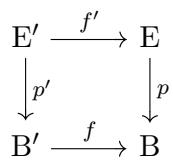
\includegraphics[keepaspectratio]{images/part001_3dd3ce93.jpg}}

一个笛卡尔方块。若 (E,p) 是局部平凡 B-纤维空间（相应地，覆叠），则 (E',p') 是以 B' 为基的局部平凡纤维空间（相应地，覆叠），且当 (E,p) 可平凡化时它亦可平凡化。

这由推论 1 得出，取其中 B = A 且 E' = B'。

推论 3. --- 设 B 为拓扑空间。设 E 与 E' 是局部平凡 B-纤维空间（相应地，覆叠）。则 \(E \times_{B} E'\) 是局部平凡 B-纤维空间（相应地，B 的覆叠）。若 E 与 E' 是可平凡化的，则它亦然。

这由推论 1 得出，取 A、B、B' 相等的情形。

命题 3. --- 设

\begin{enumerate}
\def\labelenumi{(\arabic{enumi})}
\tightlist
\item
\end{enumerate}

\pandocbounded{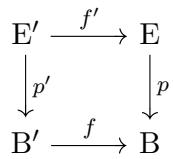
\includegraphics[keepaspectratio]{images/part001_0991252f.jpg}}

一个笛卡尔方块。假设在 B 的每一点的一个邻域内，映射 f 都有连续截面。那么，若 (E', p') 是局部平凡 B'-纤维空间（相应地，覆叠），则 B-空间 (E, p) 是局部平凡纤维空间（相应地，覆叠）。

须证 B 的每一点 \(a\) 都有邻域 U，使得 \((\mathrm{E}, p)\) 在 U 上诱导的 U-空间是局部平凡纤维空间（相应地，覆叠）。取 \(a\) 的、在其上存在连续截面 \(s\) （\(f\) 的）的一个邻域作为 U。用 \(i: \mathrm{U} \to \mathrm{B}\) 与 \(j: \overline{p}^{-1}(\mathrm{U}) \to \mathrm{E}\) 表示典范单射。由于方块 (1) 是笛卡尔的，存在唯一的连续映射 \(s^{\prime}\colon \overline{p}^{1}(\mathrm{U})\to \mathrm{E}^{\prime}\) 使得 \(f^{\prime}\circ s^{\prime} = j\) 且 \(p^{\prime}\circ s^{\prime} = s\circ p_{\mathrm{U}}\)。方块

\[
\begin{array}{c} \stackrel {{- 1}} {{p}} (\mathrm{U}) \xrightarrow {s ^ {\prime}} \mathrm{E} ^ {\prime} \\ \Biggl \downarrow p _ {\mathrm{U}} \\ \mathrm{U} \xrightarrow {s} \mathrm{B} ^ {\prime} \end{array}\tag{2}
\]

于是它是交换的，并且它与方块 (1) 的复合正是那个笛卡尔方块。

\[
\begin{array}{c} \overline {{p}} ^ {1} (\mathrm{U}) \xrightarrow {j} \mathrm{E} \\ \Biggl \downarrow p _ {\mathrm{U}} \\ \mathrm{U} \xrightarrow {i} \mathrm{B}. \end{array}
\]

由 I, p. 15 的命题 7，方块 (2) 是笛卡尔的。推论 2 使我们得以得出结论。

注意. --- 若在命题 3 中把关于映射 f 的假设减弱为只设它是普遍严格且满的，并且 \(p'\) 是覆叠，则映射 p 是平展的 (I, p. 31, prop. 8) 且是分离的 (I, p. 27, prop. 4)，但 E 不一定是 B 的覆叠。例如，可以找到拓扑空间 B、B 的局部有限闭覆盖 \((\mathrm{A}_{i})_{i\in\mathrm{I}}\) 以及一个不是覆叠的 B-空间 \((\mathrm{E},p)\)，使得对每个 \(i\in I\)，由 \(A_{i}\) 诱导的空间 \(E_{A_{i}}\) 是 \(A_{i}\) 的覆叠 (I, p. 146, exerc. 5)。但关于一个充分条件，可参见 I, p. 77 的推论 4。

\subsection{覆叠的次数}

设 B 为拓扑空间，E 为 B 的覆叠，并用 p 表示其投影。设 C 为基数 \(\operatorname{Card}(\overline{p}^{1}(b))\) （当 b 取遍 B 时）所成的集。映射 \(b \mapsto \operatorname{Card}(\overline{p}^{1}(b))\) 是 B 到 C 中的局部常值映射。若 B 非空且映射 \(b \mapsto \operatorname{Card}(\overline{p}^{1}(b))\) 是常值的，则称覆叠 E 有次数。诸基数 \(\operatorname{Card}(\overline{p}^{1}(b))\) （对 \(b \in B\)）的公共值这时称为覆叠 E 的次数，记作 \(\deg(E, p)\)，或在不致与映射 p 相混淆时，简记作 \([E:B]\) 。

若 B 非空，则以 B 为基、以 F 为纤维型的平凡覆叠有次数，等于 Card(F)。

若 B 是连通的，则函数 \(b \mapsto \text{Card}(\overline{p}^{1}(b))\) 是常值的。于是：

命题 4. --- 非空连通空间上的每个覆叠都有次数。

设 G 为拓扑空间，\((\mathrm{F}, g)\) 为 G 的覆叠，\((\mathrm{E}, f)\) 为 F 的覆叠；设这些覆叠都有次数。若 G-空间 \((\mathrm{E}, g \circ f)\) 是覆叠，则它有次数，且 \(\deg(\mathrm{E}, g \circ f) = \deg(\mathrm{F}, g) \deg(\mathrm{E}, f)\)，它也可写成

\[
[ \mathrm{E}: \mathrm{G} ] = [ \mathrm{E}: \mathrm{F} ] [ \mathrm{F}: \mathrm{G} ].
\]

事实上，若 z 是 G 的一点，则映射

\[
f _ {g (z)} ^ {- 1}: \stackrel {{- 1}} {{f}} (\stackrel {{- 1}} {{g}} (z)) \to \stackrel {{- 1}} {{g}} (z)
\]

的诸纤维都有基数 \(\deg(\mathrm{E}, f)\)，而 \(\overline{g}^1(z)\) 的基数为 \(\deg(\mathrm{F}, g)\)。于是断言由牧羊人原理 (E, III, p. 41, prop. 9) 得出。

设 B 与 B' 为拓扑空间，(E, p) 为 B 的覆叠，(E', p') 为 B' 的覆叠。设这些覆叠都有次数；则 B × B' 的覆叠 (E × E', p × p') (I, p. 71, prop. 2) 有次数，且：

\[
\deg (\mathrm{E} \times \mathrm{E} ^ {\prime}, p \times p ^ {\prime}) = \deg (\mathrm{E}, p) \deg (\mathrm{E} ^ {\prime}, p ^ {\prime}).
\]

事实上，对每个偶对 \((b,b^{\prime})\in\mathrm{B}\times\mathrm{B}^{\prime}\)，纤维 \((\mathrm{E}\times\mathrm{E}^{\prime})_{(b,b^{\prime})}\) 就是积 \(E_{b}\times E_{b^{\prime}}^{\prime}\) 。

设 B 与 B' 为拓扑空间，(E, p) 为 B 的覆叠，(E', p') 为 B' 的覆叠，并设

\[
\begin{array}{c} \mathrm{E} ^ {\prime} \xrightarrow {f ^ {\prime}} \mathrm{E} \\ \Biggl \downarrow p ^ {\prime} \\ \mathrm{B} ^ {\prime} \xrightarrow {f} \mathrm{B} \end{array}
\]

为一个笛卡尔方块。若 B′ 非空且覆叠 (E, p) 有次数，则覆叠 (E′, p′) 有次数，等于 E 的次数 (I, p. 10, cor. of prop. 4)。

\subsection{有限覆叠}

若一个覆叠的所有纤维的基数都是有限的，则称它是局部有限的。若一个覆叠的纤维的诸基数所成之集以某个有限基数为上界，则称它是有限的。

定理 1. --- 设 E、B 为拓扑空间，\(p\colon\mathrm{E}\to\mathrm{B}\) 为映射。下列条件等价：

\begin{enumerate}
\def\labelenumi{(\roman{enumi})}
\item
  赋以映射 p 的空间 E 是 B 的局部有限覆叠；
\item
  映射 p 是平展的、逆紧的且分离的；
\item
  映射 p 是连续的、开的且分离的，其纤维是有限的，且数值函数 \(b \mapsto \text{Card}(\overline{p}^{1}(b))\) 在 B 上是上半连续的 (TG, IV, p. 28)。
\end{enumerate}

在证明中将用到下面的引理：

引理. — 设 X 与 Y 为拓扑空间。映射 \(f: X \to Y\) 是闭映射，当且仅当对 Y 的每一点 y 与纤维 \(f^{-1}(y)\) 的每一邻域 W，存在 y 的邻域 V，使得 W 包含 \(f^{-1}(V)\) 。

在此陈述中，可以只考虑 \(f^{-1}(y)\) 的那些开的邻域 W。用 F 表示 W 在 X 中的补集，便可将该陈述改述如下：映射 \(f: X \to Y\) 是闭映射，当且仅当对 X 的每个闭子集 F 与 Y 的每个不属于 \(f(F)\) 的点 y，y 有与 \(f(F)\) 不相交的邻域 V。而这一断言由闭映射的定义 (TG, I, p. 30, def. 1) 立即得出。

现在来证明定理 1。三个条件中的每一个都蕴含映射 p 是连续的、开的且分离的，并且 p 的纤维是有限的。在假设 (i) 与 (iii) 之下这是显然的；在假设 (ii) 之下，p 的纤维是离散的 (I, p. 29, remark 2) 且拟紧的 (TG, I, p. 75, th. 1)，因而是有限的 (TG, I, p. 60, example 1)。

(i)⇒(ii)：只须证明 p 是逆紧的；为此，只须证明：对覆叠 (E,p) 可在其上平凡化的每个开集 U，映射 \(p_{\mathrm{U}}\colon \overline{p}^{1}(\mathrm{U})\to\mathrm{U}\) 是逆紧的 (TG, I, p. 72, prop. 3)。

由于 \(p_{U}\) 的诸纤维是有限的，这最后的断言由 TG, I, p. 77 的推论 5 得出。

(ii)⇒(iii)：设 b 为 B 的一点，并对每个 \(x \in \overline{p}^{1}(b)\)，设 \(W_{x}\) 为 x 在 E 中的开邻域，使得 \(p \mid W_{x}\) 是单射。集合 \(W = \bigcup_{x \in \overline{p}^{1}(b)} W_{x}\) 是 \(\overline{p}^{1}(b)\) 的开邻域。由于映射 p 是闭的，由上面的引理，存在 b 的开邻域 U，使得 \(\overline{p}^{1}(U) \subset W\)。对所有 \(a \in U\)，有 \(\overline{p}^{1}(a) \subset W\)；由于 p 在每个 \(W_{x}\) 上的限制是单射，由此得 \(\text{Card}(\overline{p}^{1}(a)) \leqslant \text{Card}(\overline{p}^{1}(b))\)，这就证明了映射 \(a \mapsto \text{Card}(\overline{p}^{1}(a))\) 的上半连续性。

(iii)⇒(i)：设 b 为 B 的一点。由于纤维 \(E_{b} = \overline{p}^{1}(b)\) 是有限的且映射 p 是分离的，可以对每个 \(x \in E_{b}\) 选取 x 的开邻域 \(V_{x}^{\prime}\)，使得诸 \(V_{x}^{\prime}\) 两两不相交 (I, p. 26, Remark 4)。由于映射 p 是开的且集 \(E_{b}\) 是有限的，集 \(U^{\prime} = \bigcap_{x \in E_{b}} p(V_{x}^{\prime})\) 是 b 在 B 中的开邻域。设 U 为 b 在 B 中的开邻域，含于 \(U^{\prime}\) 且使得对所有 \(a \in U\) 有 \(\text{Card}(E_{a}) \leqslant \text{Card}(E_{b})\)。对所有 \(x \in E_{b}\)，令 \(V_{x} = V_{x}^{\prime} \cap \overline{p}^{1}(U)\)。设 a 为 U 的一点；诸集 \(E_{a} \cap V_{x}\) （对 \(x \in E_{b}\)）非空且两两不相交。因而这些集中每一个都恰含一个元素，并组成 \(E_{a}\) 的一个分拆。这就证明了对每个 \(x \in E_{b}\)，映射 \(p | V_{x}\) 是单射，并且有 \(\overline{p}^{1}(U) = \bigcup_{x \in E_{b}} V_{x}\)。由于映射 p 是开的，它诱导 \(V_{x}\) 到 U 上的同胚，从而 (E, p) 是 B 的覆叠 (I, p. 70, cor. 1 of prop. 1)。

注. --- 一个连续、分离、开、逆紧且纤维有限的映射未必是覆叠。例如映射 \(x \mapsto x^{2}\) （从 R 到 \([0; +\infty[\) 的）就是这种情形。

推论 1. --- 设 E 与 B 为拓扑空间，\(p\colon\mathrm{E}\to\mathrm{B}\) 为逆紧且分离的映射。B 中使 p 在纤维 \(\mathrm{E}_{b}\) 的每一点处都是平展的那些点 b 所成的集 U 在 B 中是开的。由 (E,p) 在 U 上诱导的 U-空间是局部有限覆叠。

使映射 p 不平展的 E 的点所成的集 F 在 E 中是闭的 (I, p. 29, remark 1)。由于映射 p 是逆紧的，其像 \(p(\mathrm{F})\) 是闭的；于是 \(p(\mathrm{F})\) 的补集 U 是开的。映射 \(p_{U}\) 是分离的 (I, p. 27, prop. 4) 且逆紧的 (TG, I, p. 72, prop. 3)。按构造，映射 \(p_{\mathrm{U}}\) 是平展的；因此它满足定理 1 的条件 (ii)。

推论 2. — 设 B 为分离的拓扑空间，E 为 B-空间。设 E 是紧的且其投影 p: E → B 是平展的。则 E 是 B 的有限覆叠。

映射 \(p\) 是分离的 (I, p. 26, remark 2) 且逆紧的 (TG, I, p. 76, cor. 2)。于是由推论 1，E 是 B 的局部有限覆叠。由于 E 是紧的，\(p(\mathrm{E})\) 是 B 的拟紧子集；从 \(p(\mathrm{E})\) 到 \(\mathbb{N}\) 中的由 \(b \mapsto \operatorname{Card} \overline{p}^1(b)\) 给出的映射是局部常值的，因而有上界 (TG, IV, p. 30, corollary)。

推论 3. --- 设 B 为拓扑空间，(E,p) 与 (E',p') 为 B-空间，f: E' → E 为 B-态射。设 E' 是 B 的局部有限覆叠。

\begin{enumerate}
\def\labelenumi{\alph{enumi})}
\item
  若映射 p 是平展且分离的，则 E-空间 (E', f) 是覆叠。
\item
  若映射 f 是满的且使空间 E' 成为 E 的覆叠，则 E 是 B 的覆叠。
\end{enumerate}

在假设 \(a\) 之下，映射 \(p\) 与 \(p'\) 都是平展且分离的，且映射 \(p'\) 是逆紧的（定理 1）。于是映射 \(f\) 是平展的 (I, p. 30, cor. 1 of prop. 6)、分离的 (I, p. 25, prop. 2 b)) 且逆紧的 (I, p. 28, prop. 5)。由定理 1，\((\mathrm{E}', f)\) 是 E 的覆叠。

现在设 \(f\) 是满的，并设 \((\mathrm{E}', f)\) 是 E 的覆叠。于是它是局部有限的，故映射 \(f\) 是逆紧且满的（定理 1）。由 I, p. 25, prop. 2, c)，映射 \(p\) 是分离的，因为 \(p' = p \circ f\) 且 \(p'\) 是分离的。映射 \(p\) 是平展的 (I, p. 29, prop. 6, d))、逆紧的 (TG, I, p. 73, prop. 5, b))，且其纤维是有限的。由定理 1，B-空间 \((\mathrm{E}, p)\) 这时是 B 的覆叠。

推论 4. --- 设

\[
\begin{array}{c} \mathrm{E} ^ {\prime} \xrightarrow {f ^ {\prime}} \mathrm{E} \\ \Big \downarrow p ^ {\prime} \\ \mathrm{B} ^ {\prime} \xrightarrow {f} \mathrm{B} \end{array}
\]

为一个笛卡尔方块。设 \((\mathrm{E}^{\prime}, p^{\prime})\) 是 \(B^{\prime}\) 的局部有限覆叠，且映射 f 是普遍严格且满的。则 \((\mathrm{E}, p)\) 是 B 的局部有限覆叠。

事实上，映射 p 是平展的 (I, p. 31, prop. 8)、逆紧的 (I, p. 21, prop. 11) 且分离的 (I, p. 27, prop. 4)。

推论 5. --- 设 B 为连通的拓扑空间，(E, p) 为 B 的有限覆叠。空间 E 只有有限多个连通分支，且其中每一个都是 B 的覆叠。

若 B 是空的，结果成立；以下设 B 非空。若 X 是 E 的开闭子集，则 p 在 X 上的限制是分离的映射 (I, p. 25, prop. 2, a) 与 I, p. 26, remark 1)、平展且逆紧的 (TG, I, p. 74, corollary 1)；由定理 1，(X, p) 是 B 的局部有限覆叠。由于 B 是连通的，这个覆叠有有限次数。若 X 异于 E，则存在点 \(b \in B\) 使得 \(X_{b} \subsetneq E_{b}\)，从而 \([X:B] < [E:B]\)。由于 B 是连通的，由此得出 E 中开闭集的每个递降序列都是平稳的。

设 \(x \in E\)；于是存在含 x 的最小的开且闭的子集 X (E, III, p. 51, prop. 6)。这样的集 X 是连通的；因此它是 x 在 E 中的连通分支。这表明 E 的连通分支都是开且闭的，且其中每一个都是 B 的覆叠。由于 B 是连通的，E 的每个连通分支都与 p 的每个纤维相交；因而 E 的连通分支个数是有限的。

命题 5. — 设 B 为拓扑空间，E 与 E′ 为 B-空间，f: E′ → E 为 B-态射。设 E 是局部有限覆叠，而赋以映射 f 的空间 E′ 是局部平凡的 E-纤维空间（相应地，是覆叠）。则 E′ 是局部平凡的 B-纤维空间（相应地，是覆叠）。

用 \(p\) 与 \(p'\) 分别表示 B-空间 E 与 E' 的投影。设 \(b\) 为 B 的一点。存在 \(b\) 在 B 中的开邻域 U 以及有限分拆 \((\mathrm{V}_i)_{i\in \mathrm{I}}\) （\(\overline{p}^1 (\mathrm{U})\) 的、由 E 的开集组成的），使得对每个 \(i\in \mathrm{I}\)，映射 \(p\) 诱导 \(\mathrm{V}_i\) 到 U 上的同胚。令 \(\mathrm{V}_i' = f^{-1}(\mathrm{V}_i)\)。诸集 \(\mathrm{V}_i'\) 在 E' 中是开的，组成 \(\overline{p'}^{1}(\mathrm{U})\) 的分拆，且从 \(\mathrm{V}_i'\) 到 U 中的、由 \(p'\) 通过子空间诱导的映射使 \(V_i'\) 成为局部平凡的 U-纤维空间。由此得出，空间 \(\overline{p'}^{1}(\mathrm{U})\) 赋以映射 \(p_U': \overline{p'}^{1}(\mathrm{U}) \to U\) 后是局部平凡的 U-纤维空间 (I, p. 69, remark 2)。若 \((E', f)\) 是 E 的覆叠，则 \(p_U'\) 的纤维是离散的，因为它们与诸开集 \(V_i'\) 中每一个的交都是离散的。证明完毕。

注. --- 若 (E, p) 是 B 的覆叠且 (E', f) 是 E 的覆叠，则映射 \(p \circ f\) 是平展的 (I, p. 29, prop. 6, a)) 且分离的 (I, p. 25, prop. 2, a))。但可能发生这样的情形（见 I, p. 146 的习题 5, b)）：赋以映射 \(p \circ f\) 的空间 E′ 不是 B 的覆叠。不过参见 IV, p. 342, prop. 3。

\subsection{局部连通空间上的覆叠}

设 B 为拓扑空间，E 为 B-空间。设其投影 p 是平展且分离的映射。

若空间 B 是局部连通的，则空间 E 是局部连通的。若空间 E 是局部连通的，则 B 的开子集 \(p(\mathrm{E})\) （参看 I, p. 29, remark 2）是局部连通的。

像 \(s(\mathrm{B})\) ——这里 \(s\) 是 \(p\) 的任一截面——是开的 (I, p. 30, cor. 3) 且在 B 中是闭的 (I, p. 27, prop. 3)。若 B 是连通且非空的，则它是 E 的一个连通分支；一般地，它是 E 的若干连通分支的并。

若 B 是局部连通的，则 p 的诸截面的像的并因而是 E 的既开又闭的子集（参看 TG, I, p. 85）。

设 E 是 B 的可平凡化覆叠，\(g: E \to B \times F\) 是一个平凡化。若空间 B 是连通的，则诸集 \(V_{x} = \overline{g}^{1}(B \times \{x\})\) （当 x 取遍 F 时）就是 E 的连通分支（参看 I, p. 69 的 prop. 1）。

命题 6. --- 设 B 为拓扑空间，E 为 B-空间；用 p 表示其投影。设空间 E 是局部连通的。E 是 B 的覆叠，当且仅当 B 的每一点都有开邻域 U，使得映射 p 诱导 \(\overline{p}^{1}(U)\) 的每个连通分支到 U 上的同胚。

设 \(b\) 为 B 的一点。若 E 是 B 的覆叠，则 \(b\) 的每个连通的且使覆叠 E 在其上可平凡化的开邻域 U 都满足命题中所述的条件。反之，设 U 为满足这些条件的 \(b\) 的开邻域。集 \(\overline{p}^{1}(\mathrm{U})\) 是开的；其连通分支是 E 的开子集 (TG, I, p. 85, prop. 11) 且组成 \(\overline{p}^{1}(\mathrm{U})\) 的一个分拆。于是命题由 I, p. 70 的命题 1 的推论 1 得出。

推论 1. — 设 B 为局部连通的拓扑空间，(E,p) 为 B 的覆叠，E' 为 E 的既开又闭的子集。B-空间 (E',p \textbar{} E') 是覆叠，且 p(E') 在 B 中既开又闭。

空间 E 与 E′ 是局部连通的。对 B 的每个开子集 U，集 \(\mathrm{E}'\cap\overline{p}^{1}(\mathrm{U})\) 在 \(\overline{p}^{1}(\mathrm{U})\) 中既开又闭，因而它是 \(\overline{p}^{1}(\mathrm{U})\) 的若干连通分支的并。B 的使 p 诱导 \(\overline{p}^{1}(\mathrm{U})\) 的每个连通分支到 U 上的同胚的那些开子集 U 覆盖 B。由该命题，\(p\mid E'\) 使 \(E'\) 成为 B 的覆叠。第二个断言由此得出（参看 I, p. 68）。

推论 2. --- 设 B 为局部连通的拓扑空间，(E,p)、(E',p') 为 B 的覆叠，f,g: E' → E 为 B-态射。对 B 的每一点 b，用 \(f_b,g_b\) 表示 f 与 g 分别诱导的映射 \(\mathrm{E}_b\to \mathrm{E}_b'\) 。B 中使 \(f_b = g_b\) 的点 b 所成的集在 B 中既开又闭。

设 X 为 \(E'\) 中使 \(f(x) = g(x)\) 的点 x 所成的集。这就是 \(p'\) 到 E 中的提升 f 与 g 相重合的点所成的集；因而 X 在 \(E'\) 中既开又闭（I, p. 34 的 prop. 11）。X 的补集 Y 也是既开又闭的；于是 \(p(Y)\) 在 B 中既开又闭（推论 1）。它的补集，即 B 中使 \(f_{b} = g_{b}\) 的点 b 所成的集，因而也是既开又闭的。

推论 3. --- 设 B 为连通且局部连通的拓扑空间，(E, p) 与 (E', p') 为 B 的覆叠。对 B 的每一点 b，由 \(f \mapsto f_b\) 给出的从 \(\mathcal{C}_{\mathrm{B}}(\mathrm{E}'; \mathrm{E})\) 到 \(\mathcal{C}(\mathrm{E}_b'; \mathrm{E}_b)\) 中的映射是单射。

设 \(b\) 为 B 的一点。设 \(f\) 与 \(g\) 为从 E' 到 E 中的 B-态射，使得 \(f_b = g_b\)。B 的点 \(a\) （使 \(f_a = g_a\) 的那些）所成的集在 B 中既开又闭（推论 2）且含有 b。因而它等于 B，且 f 等于 g。

推论 4. --- 设 B 为连通且局部连通的拓扑空间，(E, p) 为 B 的覆叠，b 为 B 的一点。E 是可平凡化覆叠，当且仅当纤维 \(E_{b}\) 的每一点都属于 p 的某个连续截面的像。

该条件是必要的。设 \(E'\) 为 p 的诸连续截面的像的并，\(E''\) 为它在 E 中的补集。集 \(E'\) 在 E 中既开又闭（参看 I, p. 79）。于是 \((\mathrm{E}', p \mid \mathrm{E}')\) 是 B 的覆叠（推论 1），且由 I, p. 70 的推论 2，这个覆叠是可平凡化的。设 \(E'\) 含有 \(E_b\)，而来证明 \(E''\) 是空的。由于 \(E''\) 在 E 中既开又闭，\(p(\mathrm{E}'')\) 在 B 中既开又闭（推论 1）。由于 B 是连通的且 b 不属于 \(p(\mathrm{E}'')\)，有 \(p(\mathrm{E}'') = \varnothing\)，从而 \(E'' = \varnothing\)。

推论 5. --- 设

\pandocbounded{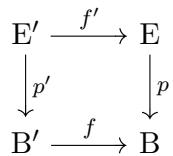
\includegraphics[keepaspectratio]{images/part001_2db9b8ac.jpg}}

为一个笛卡尔方块。设 B-空间 (E, p) 是覆叠，且空间 B' 是连通且局部连通的。设 b' 为 B' 的一点。B'-空间 (E', p') 是可平凡化覆叠，当且仅当对 E 的每个满足 \(p(x) = f(b')\) 的点 x，存在 f 的连续提升 \(g: B' \to E\)，使得 \(g(b') = x\)。

回忆 \((\mathrm{E}^{\prime}, p^{\prime})\) 是 \(B^{\prime}\) 的覆叠 (I, p. 71, cor. 2)，且映射 \(f^{\prime}\) 诱导双射 \(E_{b^{\prime}}^{\prime} \to E_{f(b^{\prime})}\) (I, p. 10, cor.)。由 I, p. 9 的 prop. 3，映射 \(s \mapsto f^{\prime} \circ s\) 定义了 \(p^{\prime}\) 的连续截面所成之集与 f 到 E 中的连续提升所成之集之间的一个双射。于是该推论由推论 4 得出。

命题 7. --- 设 B 为拓扑空间，E 与 E' 为 B-空间，f: E' → E 为 B-态射。设 E' 是 B 的覆叠且空间 B 是局部连通的。

\begin{enumerate}
\def\labelenumi{\alph{enumi})}
\item
  若 B-空间 E 的投影是平展且分离的映射，则 \((\mathrm{E}^{\prime}, f)\) 是 E 的覆叠。
\item
  若 f 是满的，则 E 是 B 的覆叠。
\end{enumerate}

用 \(p\) 与 \(p'\) 分别表示 B-空间 E 与 E′ 的投影。在假设 \(a\) 之下，\(f\) 是平展的 (I, p. 29, prop. 6, c))。在假设 \(b\) 之下，\(p\) 是平展的（同处 d)）。因此，在这两个假设的任一个之下，E 都是局部连通的；其连通分支特别在 E 中既开又闭 (TG, I, p. 85, prop. 11)。

我们先在附加假设——B 是连通且局部连通的，而 E' 是平凡覆叠 (B × F', pr₁)——之下证明命题 7。

引理. --- 若 U 是 E' 的一个连通分支，则 f 在 U 上的限制诱导 U 到 E 的某个连通分支上的同胚。

设 \(x \in F'\) 使得 \(U = B \times \{x\}\) （参看 I, p. 79）。把 \(b \in B\) 映为 \(f(b, x)\) 的从 B 到 E 中的映射是 p 的连续截面。其像 X 因而是连通的且在 E 中是开的，因为 p 是平展的 (I, p. 30, cor. 3)。而且在假设 a) 之下它还是闭的，因为 p 是分离的 (I, p. 27, prop. 3)。在假设 b) 之下它也是闭的，由 I, p. 80 的推论 1，因为 U 在 E' 中既开又闭。于是 X 是 E 的一个连通分支。

由于 \(f \mid \mathrm{U} \colon \mathrm{U} \to \mathrm{X}\) 是双射且是开的，它是到其像上的同胚，这就证明了引理。

保留引理前面的假设，现在来证明断言 \(a\) )。设 V 为 E 的一个连通分支。它是 E 中的既开又闭集，而 \(f^{-1}(\mathrm{V})\) 是 \(\mathrm{E}'\) 的若干连通分支的并，由引理，\(f\) 把这些分支同胚地映到 V 上。由 I, p. 79 的 prop. 6 得出 \((\mathrm{E}', f)\) 是覆叠。

来证明 b)。由于 f 是满的，由引理得出 E 的每个连通分支 V 都是某个连通分支 \(U = B \times \{x\}\) （\(E'\) 的）的同胚像。于是映射 p 诱导 V 到 B 上的同胚。由 prop. 6，E 是 B 的覆叠。

这就在附加假设——B 是连通的且 E' 是 B 的可平凡化覆叠——之下证明了命题。来证明一般情形。

存在 B 的由连通开集组成的覆叠 \((\mathrm{U}_{i})_{i\in\mathrm{I}}\)，覆叠 \(E'\) 在这些开集上均可平凡化。设 \(i\in I\) 。

来证明 \(a\)。若映射 \(p\) 是平展且分离的，则映射 \(p_{\mathrm{U}_i}\colon \mathrm{U}_i\times_{\mathrm{B}}\mathrm{E}\to \mathrm{U}_i\) （对 \(i\in \mathrm{I}\)）同样如此，这由 I, p. 31 的 prop. 8 与 I, p. 27 的 prop. 4 得出。于是由已处理的特殊情形得出，对每个 \(i\in \mathrm{I}\)，\(\mathrm{U}_i\)-空间 \((\overline{p'}^{1}(\mathrm{U}_i),f_{\mathrm{U}_i})\) 是覆叠。用 A 表示不交并 \(\coprod_{i\in I}\mathrm{U}_i\) 的全空间，用 \(q\colon \mathrm{A}\to \mathrm{B}\) 表示典范映射。于是，空间 \(\mathrm{A}\times_{\mathrm{B}}\mathrm{E}'\) （赋以映射 \(f_{\mathrm{A}}\colon \mathrm{A}\times_{\mathrm{B}}\mathrm{E}'\to \mathrm{A}\times_{\mathrm{B}}\mathrm{E}\) 的）是 \(\mathrm{A}\times_{\mathrm{B}}\mathrm{E}\) 的覆叠。映射 \(q\) 在 B 的每一点的邻域内都有连续截面，而把 I, p. 72 的命题 3 应用于笛卡尔方块

\[
\begin{array}{c} \mathrm {A\times_ {B} E^ {\prime}} \longrightarrow \mathrm {E^ {\prime}} \\ \Big \downarrow f _ {\mathrm{A}} \\ \mathrm {A\times_ {B} E} \longrightarrow \mathrm{E} \end{array} ,
\]

蕴含 \(E'\) 是 E 的覆叠。

来证明 \(b\)。设 \(f\) 是满的。于是对 I 的每个元素 \(i\)，映射 \(f_{\mathrm{U}_i}\colon \mathrm{U}_i\times_{\mathrm{B}}\mathrm{E}'\to \mathrm{U}_i\times_{\mathrm{B}}\mathrm{E}\) 是满的，且空间 \(\mathrm{U}_i\times_{\mathrm{B}}\mathrm{E}'\) （赋以映射 \(f_{\mathrm{U}_i}\) 的）是 \(\mathrm{U}_i\times_{\mathrm{B}}\mathrm{E}\) 的覆叠 (I, p. 71, cor. 2 of prop. 2)。由前面处理的特殊情形得出，\(\mathrm{U}_i\)-空间 \((\overline{p}^{1}(\mathrm{U}_{i}),p_{\mathrm{U}_{i}})\) 是覆叠。从而 E 是 B 的覆叠。

设 B 为拓扑空间，E 与 E′ 为 B 的覆叠，\(f: E \rightarrow E'\) 为 B-态射。我们已经看到，在下列两个假设的每一个之下，\((E, f)\) 都是覆叠：1) 覆叠 E 是局部有限次的 (I, p. 76, cor. 1)；2) 空间 B 是局部连通的 (I, p. 81, prop. 7)。这一现象可以解释如下。

设 F 与 F′ 为离散拓扑空间，\(f: B \times F \to B \times F'\) 为 B-态射。由 \(\widetilde{f}: b \mapsto \mathrm{pr}_{2} \circ f(b, \cdot)\) 给出的从 B 到空间 \(\mathcal{C}_{c}(F; F')\) 中的映射是连续的 (TG, X, p. 28, th. 3)。若 U 是 B 的开子集且映射 \(\widetilde{f}\) 在 U 上是常值的，则由 f 诱导出的映射 \(f_{U}: U \times F \to U \times F'\) 是可平凡化覆叠 (I, p. 69, prop. 1)。

空间 \(\mathcal{C}_c(\mathrm{F};\mathrm{F}')\) 无非就是映射所成之集 \(\mathcal{F}(\mathrm{F};\mathrm{F}')\) （从 F 到 \(\mathrm{F}'\) 中的），赋以经由典范同构由积空间 \((\mathrm{F}')^{\mathrm{F}}\) 的拓扑所诱导的拓扑。对这个拓扑，空间 \(\mathcal{F}(\mathrm{F};\mathrm{F}')\) 是全不连通的 (I, p. 84, prop. 10)。于是，若空间 B 是连通的，则映射 \(\widetilde{f}\) 是常值的 (I, p. 82, prop. 4)；若空间 B 是局部连通的，则映射 \(\widetilde{f}\) 是局部常值的。当集 F 有限时，空间 \(\mathcal{F}(\mathrm{F};\mathrm{F}')\) 是离散的，而映射 \(\widetilde{f}\) 是局部常值的。

注. --- 设 B 为拓扑空间，\((\mathrm{E}, p)\) 与 \((\mathrm{E}', p')\) 为 B-空间，\(f: E' \to E\) 为 B-态射。

\begin{enumerate}
\def\labelenumi{\alph{enumi})}
\item
  若 E 与 E' 是 B 的覆叠，则映射 f 是平展的 (I, p. 29, prop. 6) 且分离的 (I, p. 25, prop. 2)。但若空间 B 不是局部连通的，则一般而言 (E', f) 未必是 E 的覆叠 (I, p. 145, exerc. 4)。
\item
  若 \((\mathrm{E}^{\prime}, p^{\prime})\) 是 B 的覆叠，f 是满的且使 \(E^{\prime}\) 成为 E 的覆叠，则映射 p 是平展的 (I, p. 29, prop. 6)。但若空间 B 不是局部连通的，则一般而言它未必是分离的 (I, p. 145, exerc. 4)。特别地，E 未必是 B 的覆叠。
\end{enumerate}

推论. --- 设 B 为连通且局部连通的拓扑空间。设 E 与 E' 为 B 的覆叠。设 b 为 B 的一点。设 \(f: E' \to E\) 为 B-态射，\(f_{b}: E_{b}' \to E_{b}\) 为 f 通过限制到纤维上所诱导的映射。若映射 \(f_{b}\) 是单射（相应地，满射，相应地，双射），则映射 f 亦然。

用 \(p\) 表示 B-空间 E 的投影。由该命题，\((\mathrm{E}', f)\) 是 E 的覆叠；其像 \(f(\mathrm{E}')\) 在 E 中既开又闭。用 U 表示 \(f(\mathrm{E}')\) 在 E 中的补集，于是 B-空间 \((\mathrm{U}, p \mid \mathrm{U})\) 是 B 的覆叠 (I, p. 80, corollary 1)。若映射 \(f_b\) 是满的，则这个覆叠在 \(b\) 处的纤维是空的。由于 B 是连通空间，这时 U 是空的，故 \(f\) 是满的。

E 中使 f 的纤维恰含一个元素的点所成的集 V 是既开又闭的。B-空间 \((V, p|V)\) 与 \((f(E'), p|f(E'))\) 是 B 的覆叠（同处），且典范映射 \(i: V \to f(E')\) 是 B-态射。若映射 \(f_b\) 是单射，则映射 \(i_b\) 是满的，故由前述结果 i 是满的，从而 \(V = f(E')\)。于是映射 f 是单射。

\subsection{仿紧空间上的覆叠}

命题 8. --- 仿紧空间 (I, p. 69) 上的覆叠是仿紧空间。

先证明一个引理。

引理. --- 设 E 为分离的拓扑空间。设 E 有局部有限开覆盖 \((\mathrm{V}_{i})_{i\in\mathrm{I}}\)，使得对每个 \(i\in I\)，\(\overline{V_{i}}\) 都是仿紧空间。则空间 E 是仿紧的。

设 \((\mathrm{W}_{j})_{j\in\mathrm{J}}\) 为 E 的开覆盖；我们来证明存在 E 的局部有限开加细 \((\mathrm{A}_{k})_{k\in\mathrm{K}}\)，它比覆盖 \((\mathrm{W}_{j})_{j\in\mathrm{J}}\) 更细。对所有 \(i\in I\)，设 \((\mathrm{A}_{\ell}^{\prime})_{\ell\in\mathrm{K}_{i}}\) 为 \(\overline{V_{i}}\) 的由 \(\overline{V_{i}}\) 的开子集组成的局部有限覆盖，比覆盖 \((\mathrm{W}_{j}\cap\overline{\mathrm{V}_{i}})_{j\in\mathrm{J}}\) 更细。设 K 为族 \((\mathrm{K}_{i})_{i\in\mathrm{I}}\) 的和 (E, II, p. 30, def. 8)。对 K 的每个元素 \(k=(\ell,i)\)，令 \(A_{k}=A_{\ell}^{\prime}\cap V_{i}\)。于是 \(A_{k}\) 在 E 中是开的，且有 \(\bigcup_{k\in K}A_{k}=\bigcup_{i\in I}V_{i}=E\)；此外，对每个 \(k\in K\)，存在指标 \(j\in J\)，使得 \(A_{k}\subset W_{j}\)。于是族 \((\mathrm{A}_{k})_{k\in\mathrm{K}}\) 是 E 的比 \((\mathrm{W}_{j})_{j\in\mathrm{J}}\) 更细的开覆盖。剩下要证明族 \((\mathrm{A}_{k})_{k\in\mathrm{K}}\) 是局部有限的。设 \(x\in E\)；存在开邻域 U （x 的），它只与那些 \(V_{i}\) （其 i 属于 I 的有限子集 I'）相交。对每个 \(i\in I'\)，x 有开邻域 \(U_{i}\subset U\)，它只与有限多个开集 \(A_{k}\) （对 \(k\in K_{i}\times\{i\}\)）相交：若 x 不属于 \(\overline{V_{i}}\)，这是显然的；而若 x 属于 \(\overline{V_{i}}\)，这由覆盖 \((\mathrm{A}_{\ell}^{\prime})_{\ell\in\mathrm{K}_{i}}\) （\(\overline{V_{i}}\) 的）的局部有限性质得出。于是 \(V^{\prime}=\bigcap_{i\in I'}U_{i}\) 是 x 的开邻域，它只与诸 \(A_{k}\) （\(k\in K\)）中的有限多个相交，从而覆盖 \((\mathrm{A}_{k})_{k\in\mathrm{K}}\) 是局部有限的。

来证明该命题。设 E 为 B 的覆叠，用 p 表示其投影，并设空间 B 是仿紧的。设 \((\mathrm{A}_{i})_{i\in\mathrm{I}}\) 为 B 的局部有限开覆盖，使得对每个 \(i\in I\)，覆叠 E 在 \(A_{i}\) 上可平凡化。对所有 \(i\in I\)，设 \(F_{i}\) 为离散拓扑空间，并设 \(g_{i}\colon\overline{p}^{1}(\mathrm{A}_{i})\to\mathrm{A}_{i}\times\mathrm{F}_{i}\) 为 E 在 \(A_{i}\) 上的一个平凡化。设 \((\mathrm{B}_{i})_{i\in\mathrm{I}}\) 为 B 的开覆盖，使得对每个 \(i\in I\)，有 \(\overline{B_{i}}\subset A_{i}\) (TG, IX, p. 49, prop. 4 与 p. 48, cor. 1)。对每个 \(i\in I\)，令 \(V_{i}=\overline{p}^{1}(\mathrm{B}_{i})\)；我们有 \(\overline{V_{i}}\subset\overline{p}^{1}(\overline{\mathrm{B}_{i}})\subset\overline{p}^{1}(\mathrm{A}_{i})\) 以及 \(V_{i}=\overline{g_{i}}^{1}(\mathrm{B}_{i}\times\mathrm{F}_{i})\)，从而 \(\overline{V_{i}}\subset\overline{g_{i}}^{1}(\overline{\mathrm{B}_{i}}\times\mathrm{F}_{i})\)。由于 B 是仿紧的，\(\overline{B_{i}}\) 是仿紧的 (TG, I, p. 69, prop. 16)，且 \(\overline{B_{i}}\times F_{i}\) 是仿紧的 (TG, I, p. 70, prop. 18)。于是 \(\overline{g_{i}}^{1}(\overline{\mathrm{B}_{i}}\times\mathrm{F}_{i})\) 是仿紧的，从而 \(\overline{V_{i}}\) 也是仿紧的 (TG, I, p. 69, prop. 16)。族 \((\mathrm{V}_{i})_{i\in\mathrm{I}}\) 按构造是 E 的局部有限开覆盖。最后，空间 E 是分离的 (I, p. 26, remark 3)。因此它满足引理的假设，由此得出命题。

注. --- 可以证明，可度量化空间上的覆叠是可度量化的 (I, p. 145, exerc. 1)，而局部紧且无穷可数空间上的连通覆叠本身是局部紧且无穷可数的 (I, p. 145, exerc. 2)。

\subsection{局部常值层}

设 B 为拓扑空间，F 为一个集；给 F 赋以离散拓扑。称以 F 为茎型的 B 上常值层为 B 上以 F 为值的局部常值函数所成的层 (I, p. 45, example 2)。当不致担心与空间 B 相混淆时，这个层有时记作 \(\underline{\mathbf{F}}\)。它与平展 B-空间 \((B \times F,\mathrm{pr}_1)\) 的连续截面在 B 上所成的层相恒同：公式 \(i([U,s,a]) = (a,s(a))\) 确实定义了一个典范同构 \(i\) （从与 \(\underline{\mathbf{F}}\) 相伴的平展空间到 \((B \times F,\mathrm{pr}_1)\) 上的）。对每个 \(a \in B\)，映射 \([U,s,a] \mapsto s(a)\) 是茎 \(\underline{\mathbf{F}}_a\) （\(\underline{\mathbf{F}}\) 在 \(a\) 处的）到集 F 上的典范双射。

设 \(\mathcal{P} = (\mathcal{P}(\mathrm{U}), r_{\mathrm{UV}})\) 为 B 上的预层，使得对 B 的每个开集 U 有 \(\mathcal{P}(\mathrm{U}) = \mathrm{F}\)，且对 B 的每对开集 (U, V) 有 \(r_{\mathrm{UV}} = \mathrm{Id}_{\mathrm{F}}\) （只要 \(\mathrm{U} \subset \mathrm{V}\)）。于是，层 \(\widetilde{\mathcal{P}}\) （与 \(\mathcal{P}\) 相伴的）典范地同构于常值层 \(\underline{\mathrm{F}}\) (I, p. 52, example 1)。

定义 3. --- 拓扑空间 B 上的层 \(\mathcal{F}\) 是局部常值的，如果 B 的每一点都有开邻域 U，使得诱导层 \(\mathcal{F} \mid U\) 同构于 U 上的一个常值层。

命题 9. --- 一个层是局部常值的，当且仅当与之相伴的平展空间是覆叠。

设 B 为拓扑空间，\(\mathcal{F}\) 为 B 上的层。层 \(\mathcal{F}\) 是常值的，当且仅当平展空间 \(\mathrm{E}_{\mathcal{F}}\) B-同构于平凡覆叠 \((\mathrm{B} \times \mathrm{F},\mathrm{pr}_1)\)，其中 F 是离散拓扑空间。若 U 是 B 的开子集，则与诱导层 \(\mathcal{F} \mid \mathrm{U}\) 相伴的平展空间与 \(\mathrm{E}_{\mathcal{F}}\) 在 U 上诱导的 U-平展空间相恒同（参看 I, p. 51）。命题由此得出。

推论. --- 一个平展 B-空间是覆叠，当且仅当其截面的层是局部常值的。

这由该命题以及 I, p. 52 的例 2 得出。

\subsection{局部常值层的积}

设 B 为拓扑空间，\((\mathcal{F}_{i})_{i\in\mathrm{I}}\) 为 B 上的一个层族。用 \(\mathcal{F}\) 表示积层 \(\prod_{i\in I}\mathcal{F}_{i}\)，并对 \(i\in I\)，设 \(pr_{i}\colon \mathcal{F}\to\mathcal{F}_{i}\) 为指标 i 的投影态射 (I, p. 46, example 7)。设 \((\mathrm{E},p)\) 与 \((\mathrm{E}_{i},p_{i})\) 为分别与层 \(\mathcal{F}\) 和 \(\mathcal{F}_{i}\) 相伴的平展 B-空间，并设 \(\varphi_{i}\colon \mathrm{E}\to \mathrm{E}_{i}\) 为与 \(pr_{i}\) 相伴的 B-态射 (I, p. 50)。最后，用 \((\mathrm{E}^{\prime},p^{\prime})\) 表示 B-积 \(\prod_{B}\mathrm{E}_{i}\)。由 B-空间积的泛性质 (I, p. 5)，存在唯一的 B-态射 \(\Phi\colon \mathrm{E}\to \mathrm{E}^{\prime}\)，使得对每个 \(i\in I\)，有 \(pr_{i}\circ\Phi=\varphi_{i}\)。

命题 10. --- 若集 I 是有限的，则 B-态射 \(\Phi\) 是同构。

由 I, p. 32 的推论，B-空间 \(\mathrm{E}'\) 是平展的，于是只须证明 B-态射 \(\Phi\) 是双射 (I, p. 30, cor. 2)。对 B 的每一点 b，限制 \(\Phi_b\colon \mathrm{E}_b\to \mathrm{E}'_b\) （\(\Phi\) 在 b 处纤维上的）与从 \(\varinjlim\prod_{i\in I}\mathcal{F}_{i}(U)\) 到 \(\prod_{i\in I}\varinjlim\mathcal{F}_{i}(U)\) 的典范映射相恒同，其中 U 取遍 B 的含 b 的开子集（参看 I, p. 50）。由 E, III, p. 67 的 prop. 10，这个映射是双射。

现在考虑拓扑空间 B 上局部常值层的情形。设 \((\mathrm{F}_{i})_{i\in\mathrm{I}}\) 为一个集族，并令 \(F=\prod_{i\in I}F_{i}\) 。如下定义典范态射 \(\psi=(\psi_{\mathrm{U}})\) （从常值层 \(\underline{F}\) 到积 \(\prod_{i\in I}\underline{F}_{i}\) （诸常值层 \(\underline{F}_{i}\) 的）中的）：对 B 的每个开子集 U 与每个局部常值函数 \(f\colon U\to F\) ，令 \(\psi_{\mathrm{U}}(f)=(\mathrm{pr}_{i}\circ f)_{i\in\mathrm{I}}\) 。

命题 11. --- 若集 I 是有限的，或空间 B 是局部连通的，则典范态射 \(\psi\colon\underline{\mathbf{F}}\to\prod\underline{\mathbf{F}_{i}}\) 是同构。

设 U 为 B 的开子集。显然映射 \(\psi_{\mathrm{U}}\) 是单射。来证明它是满射。只须证明：对每个族 \((f_i)_{i\in \mathrm{I}}\) （其中 \(f_{i}\) 是从 U 到 \(\mathrm{F}_i\) 中的局部常值映射）以及 U 的每一点 \(a\)，存在 \(a\) 在 U 中的邻域 V，使得对每个 \(i\in \mathrm{I}\)，映射 \(f_{i}|\mathrm{V}\) 都是常值的。当集 I 有限时，这样一个邻域的存在性是显然的。当空间 B 局部连通时，只须取 V 为 \(a\) 在 U 中的连通邻域。这就证明了命题。

推论 1. --- 局部常值层的有限积是局部常值的。

设 \((\mathcal{F}_{i})_{i\in\mathrm{I}}\) 为 B 上的局部常值层的有限族。B 的每一点 a 都有 B 中的开邻域 U，使得对每个 \(i\in I\)，层 \(\mathcal{F}_{i}\mid U\) 同构于常值层。于是这对层 \((\prod\mathcal{F}_{i})\mid U\) 也成立，后者等于 \(\prod(\mathcal{F}_{i}\mid U)\)。

推论 2. --- 设 \((\mathcal{F}_{i})_{i\in I}\) 为 B 上的层族。设空间 B 是局部连通的，且 B 的每一点都有开邻域 U，使得对每个 \(i\in I\) ，层 \(\mathcal{F}_{i}|U\) 同构于常值层。则积层 \(\prod \mathcal{F}_{i}\) 是局部常值的。

注. --- 1) 设 \((\mathrm{E}_{i}, p_{i})_{i \in \mathrm{I}}\) 为拓扑空间 B 的覆叠族。设空间 B 是局部连通的，且存在 B 的开覆盖 \((\mathrm{U}_{j})_{j \in \mathrm{J}}\)，使得对每个 \(j \in J\) 与每个 \(i \in I\)，覆叠 \(E_{i}\) 在 \(U_{j}\) 上均可平凡化。对 \(i \in I\)，设 \(F_{i}\) 为 \(E_{i}\) 的截面的局部常值层，设 \(F\) 为积层 \(\prod_{i} F_{i}\) 。由前一个推论，F 是局部常值层，因而与之相伴的平展 B-空间 E 是覆叠 (I, p. 86, prop. 8)。对 \(i \in I\)，设 \(pr_{i}: E \to E_{i}\) 为由指标 i 的投影态射 \(F \to F_{i}\) 诱导的 B-态射。

现在考虑 B 的一个覆叠 (Y, q)，且对每个 \(i \in I\)，设 \(f_i \colon Y \to E_i\) 为 B-态射。若用 G 表示 q 的截面的局部常值层，则诸 B-态射 \(f_i\) 诱导层态射 \(\widetilde{f}_i \colon G \to F_i\) 。设 \(\widetilde{f} \colon G \to F\) 为唯一的层态射，使得 \(\widetilde{f}_i = pr_i \circ \widetilde{f}\) 对所有 \(i \in I\) 成立。于是存在唯一的 B-态射 \(f \colon Y \to E\)，使得对每个 i 有 \(f_i = pr_i \circ f\)：它就是诱导 \(\widetilde{f}\) 的那个 B-态射。

有时称 E 为族 \((\mathrm{E}_i)_{i\in \mathrm{I}}\) 的积覆叠。

\begin{enumerate}
\def\labelenumi{\arabic{enumi})}
\setcounter{enumi}{1}
\tightlist
\item
  沿用前面的记号，典范 B-态射 \(\Phi\colon\mathrm{E}\to\Pi_{\mathrm{B}}\mathrm{E}_{i}\) 是双射。事实上该问题在 B 上是局部性的，故可设对每个 \(i\in\mathrm{I}\)，B-空间 \(\mathrm{E}_{i}\) 同构于 B-空间 \((\mathrm{B}\times\mathrm{F}_{i},\mathrm{pr}_{1})\)，其中 \(\mathrm{F}_{i}\) 是离散拓扑空间，从而层 \(\mathcal{F}_{i}\) 同构于层 \(\underline{\mathrm{F}}_{i}\)。由 prop. 11，层 \(\mathcal{F}\) 与层 \(\underline{\mathrm{F}}\) 相恒同，其中 \(\mathrm{F}\) 是集 \(\prod\mathrm{F}_{i}\)，赋以离散拓扑，且映射 \(\Phi\) 与典范映射 \(B \times F \rightarrow B \times (\prod_{i} F_{i})\) 相恒同，后者是双射。
\end{enumerate}

\subsection{局部连通空间上局部常值层的态射}

设 B 为拓扑空间，\((\mathrm{E},p)\) 与 \((\mathrm{E}^{\prime},p^{\prime})\) 为 B-空间。用 \(\mathcal{M} = \underline{\mathcal{M}or_{\mathrm{B}}(\mathrm{E};\mathrm{E}^{\prime})}\) 表示从 \((\mathrm{E},p)\) 到 \((\mathrm{E}^{\prime},p^{\prime})\) 中的 B-态射在 B 上所成的层 (I, p. 45, example 4)。若 U 是 B 的开集而 b 是 U 的一点，我们用 \(\theta_{b,\mathrm{U}}\colon\mathcal{M}(\mathrm{U})\to\mathcal{C}(\mathrm{E}_{b};\mathrm{E}_{b}^{\prime})\) 表示通过过渡到 b 处的纤维而得到的典范映射。我们用 \(\theta_{b}\colon\mathcal{M}_{b}\to\mathcal{C}(\mathrm{E}_{b};\mathrm{E}_{b}^{\prime})\) 表示唯一的映射，使得对 B 的每个含 b 的开集 U，\(\theta_{b,\mathrm{U}}\) 都是 \(\theta_{b}\) 与典范映射 \(\mathcal{M}(\mathrm{U})\to\mathcal{M}_{b}\) 的复合 (E, III, p. 62)。

再设 \(\mathcal{I} = \underline{\mathcal{I}som}_{\mathrm{B}}(\mathrm{E};\mathrm{E}^{\prime})\) 为从 \((\mathrm{E},p)\) 到 \((\mathrm{E}^{\prime},p^{\prime})\) 中的 B-同构在 B 上所成的层。用 \(i\colon \mathcal{I}\to \mathcal{M}\) 表示典范态射。对每个 \(b\in \mathrm{B}\)，映射 \(\theta_{b}\circ i_{b}\) 诱导映射 \(\theta_b^\prime\) ，它把 \(\mathcal{I}_b\) 映到由 \(\mathrm{E}_b\) 到 \(\mathrm{E}_b^\prime\) 上的连续双射所成之集中。

命题 12. --- 设空间 B 是局部连通的且 B-空间 E 与 E' 是覆叠。于是层 \(\mathcal{M}or_{\mathrm{B}}(\mathrm{E};\mathrm{E}')\) 是局部常值的，且对每个 \(b\in\mathrm{B}\)，映射 \(\theta_{b}\) 是从其在 \(b\) 处的茎到从 \(\mathrm{E}_{b}\) 到 \(\mathrm{E}_{b}^{\prime}\) 中的映射所成之集上的双射。

类似地，层 \(\mathcal{I}\text{som}_{\mathrm{B}}(\mathrm{E};\mathrm{E}^{\prime})\) 是局部常值的，且对 B 的每一点 \(b\)，映射 \(\theta_{b}^{\prime}\) 是从其在 \(b\) 处的茎到从 \(\mathrm{E}_{b}\) 到 \(\mathrm{E}_{b}^{\prime}\) 上的双射所成之集上的双射。

我们将用 \(\mathcal{M} = \underline{\mathcal{M}or}_{\mathrm{B}}(\mathrm{E};\mathrm{E}^{\prime})\) 与 \(\mathcal{I} = \underline{\mathcal{Isom}}_{\mathrm{B}}(\mathrm{E};\mathrm{E}^{\prime})\) 表示。要证的断言在 B 上是局部性的；因此可设 \(\mathrm{E} = \mathrm{B}\times \mathrm{F}\) 与 \(\mathrm{E}' = \mathrm{B}\times \mathrm{F}'\) 是平凡覆叠，其中 F 与 \(\mathrm{F}'\) 是离散拓扑空间。

首先来证明，对 B 的每个连通开子集 U 与 U 的每一点 b，映射 \(\theta_{b,U}\) 是双射。设 \(f\colon U\times F\to U\times F'\) 为 U-空间的态射；于是 \(\theta_{b,U}(f)\) 是映射 \(y\mapsto\mathrm{pr}_{2}(f(b,y))\) （从 F 到 \(F'\) 中的）。对所有 \(y\in F\)，映射 \(x\mapsto\mathrm{pr}_{2}(f(x,y))\) 是从连通空间 U 到离散空间 \(F'\) 中的连续映射，故为常值的，等于 \(\mathrm{pr}_{2}(f(b,y))\)。于是有 \(f(x,y)=(x,\theta_{b,U}(f)(y))\)。由此得出 \(\theta_{b,U}\) 是双射；

其逆双射把每个映射 \(\varphi\colon\mathrm{F}\to\mathrm{F}^{\prime}\) 对应到从 \(\mathrm{U}\times\mathrm{F}\) 到 \(\mathrm{U}\times\mathrm{F}^{\prime}\) 中的、由 \((x,y)\mapsto(x,\varphi(y))\) 给出的 U-态射。

按假设，每点 \(b \in B\) 都有由连通开邻域组成的基本邻域系；于是映射 \(\theta_{b}\) 是双射。诸映射 \(\theta_{b,\mathrm{U}}^{-1}\) （其中 U 取 B 的非空连通开子集而 b 取 B 的任意点）定义了从以 \(F^{\prime F}\) 为茎型的常值层到层 \(\mathcal{M}\) 的一个预层态射（关于 B 的连通开子集组成的基）。由前所证，这个态射诱导茎上的双射；因而它是同构。

关于层 \(\mathcal{I}\) 的断言类似地证明。

推论 1. --- 设 B 为拓扑空间，A 为 B 的子空间。设空间 A 与 B 都是局部连通的。设 E 与 E' 为 B 的覆叠。则典范态射 \(\psi\colon\mathcal{M}or_{B}(E;E')_{A}\to\mathcal{M}or_{A}(E_{A};E'_{A})\) 与 \(\psi'\colon\mathcal{I}som_{B}(E;E')_{A}\to\mathcal{I}som_{A}(E_{A};E'_{A})\) (I, p. 45, example 4) 都是同构。

对每点 \(a \in \mathrm{A}\)，由前一个命题以及 I, p. 63 的例 2（应用于空间 \(\{a\}\)、A、B 及典范单射）得出，典范态射 \(\psi\) 通过过渡到茎诱导 \(\mathrm{E}_a^{\mathrm{E}_a'}\) 上的恒同映射。因而它是同构。\(\psi'\) 是同构这一事实类似地证明。

推论 2. --- 设 B 为拓扑空间，A 为 B 的子空间。设空间 A 与 B 都是局部连通的，且偶对 (B, A) 满足 I, p. 37 的性质 (PCV)。设 E 与 E' 为 B 的覆叠，用 p 与 p' 表示它们的投影。设 \(g: \overline{p}^{1}(A) \to (\overline{p}')^{1}(A)\) 为 A-态射（相应地，A-同构）。则存在 A 在 B 中的邻域 U 以及 U-态射（相应地，U-同构）\(f: \overline{p}^{1}(U) \to (\overline{p}')^{1}(U)\)，使得 \(f_{A} = g\)。

保留推论 1 的记号。由同一推论，A-态射 \(g \colon \mathrm{E}_{\mathrm{A}} \to \mathrm{E}_{\mathrm{A}}^{\prime}\) 与截面 \(s_0\) （平展空间 \(\mathrm{E}_{\mathcal{M}}\) （与 \(\mathcal{M}\) 相伴的）在 A 上的）相恒同。由对偶对 (B, A) 所作的假设以及 I, p. 39 的引理 3，存在 A 在 B 中的开邻域 U 以及连续截面 \(s\) （\(\mathrm{E}_{\mathcal{M}}\) 在 U 上的、延拓 \(s_0\) 的）。这个截面 \(s\) 与一个 U-态射 \(f \colon \mathrm{E}_{\mathrm{U}} \to \mathrm{E}_{\mathrm{U}}^{\prime}\) （延拓 \(g\) 的）相恒同。

g 是 A-同构的情形类似处理，只需把层 M 换成层 S。

\section{主覆叠}

\subsection{主纤维丛}

定义 1. --- 设 G 为拓扑群，B 为拓扑空间。以 B 为基、以 G 为群的（右）主纤维丛是指赋以 G 在 E 上的右作用 (A, I, p. 50) 且满足下列性质的 B-空间 (E, p)：

(FP) 对每一点 \(b\) （\(B\) 的），存在邻域 \(U\) （\(b\) 的）以及 U-同构 \(f\colon U\times G\to \overline{p}^{1}(U)\)，使得对所有 \(u\in U\) 与 \(g,g'\in G\)，有 \(f(u,gg')=f(u,g)\cdot g'\)。

我们有时不说 \((E, p)\) 是以 B 为基、以 G 为群的主纤维丛，而说四元组 \((E, G, B, p)\) 是一个主纤维化（参看 VAR, R, §6），或者滥用术语，说映射 \(p: E \to B\) 是以 B 为基、以 G 为群的主纤维化。

当基 B、群 G 以及 G 在 E 上的作用都确定无疑时，我们就简单地说 \((E, p)\) 是主纤维丛。

设 G 为拓扑群。设 \((E,p)\) 为赋以 G 的左作用的 B-空间。若对于与给定运算相反的群 \(G^{\circ}\) 的右作用 (A, I, p. 50)，\((E,p)\) 是以 \(G^{\circ}\) 为群的主右纤维丛，则称 \((E,p)\) 是以 G 为群的主左纤维丛。

主纤维丛是局部平凡的纤维丛 (I, p. 68, def. 1)。

由性质 (FP) 得出，群 G 连续地 (TG, III, p. 9) 且自由地作用在 E 上，且这个作用的轨道就是 B-空间 (E, p) 的纤维。映射 \(p' \colon \mathrm{E} / \mathrm{G} \to \mathrm{B}\) （由 \(p\) 导出的）是连续的双射。同样由性质 (FP)，映射 \(p\) 是开的 (TG, I, p. 30, prop. 2 与 p. 26, prop. 5)；于是 \(p'\) 是同胚 (TG, I, p. 32, prop. 3)。

设 \((\mathrm{E},p)\) 与 \((\mathrm{E}^{\prime},p^{\prime})\) 为以 B 为基、以 G 为群的主纤维丛。我们称映射 \(f: E \to E^{\prime}\) 为（以 B 为基、以 G 为群的）主纤维丛的态射，如果 f 是 B-态射，且有 \(f(x \cdot g) = f(x) \cdot g\) （对所有 \(x \in E\) 与每个 \(g \in G\)）。设 \((\mathrm{E}^{\prime\prime},p^{\prime\prime})\) 为以 B 为基、以 G 为群的主纤维丛。若 \(f: \mathrm{E} \to \mathrm{E}'\) 与 \(g: \mathrm{E}' \to \mathrm{E}''\) 都是主纤维丛的态射，则映射 \(g \circ f: \mathrm{E} \to \mathrm{E}''\) 是主纤维丛的态射。按照一般定义 (E, IV, p. 11)，可以把上面定义的那些取作以 B 为基、以 G 为群的主纤维丛结构的态射。我们用 \(\mathcal{C}_{\mathrm{B}}^{\mathrm{G}}(\mathrm{E}; \mathrm{E}')\) 表示从 \((\mathrm{E}, p)\) 到 \((\mathrm{E}',p')\) 中的主纤维丛态射所成之集。

我们称以 B 为基、以 G 为群的平凡主纤维丛为 B-空间 \((B \times G, pr_{1})\) （赋以 G 在 \(B \times G\) 上的由 \((b, g) \cdot h = (b, gh)\) 定义的右作用）。

以 B 为基、以 G 为群的主纤维丛 (E, p) 称为可平凡化的，如果存在从 (E, p) 到平凡主纤维丛 \((B \times G,\mathrm{pr}_{1})\) 上的同构；这样的同构称为主纤维丛 (E, p) 的平凡化。性质 (FP) 表达的是：存在 B 的开覆盖 \((\mathrm{U}_{i})_{i \in \mathrm{I}}\)，使得对每个 \(i \in I\)，赋以由 G 在 E 上的作用所诱导的 G 的右作用的 \(\mathrm{U}_{i}\)-空间 \((\overline{p}^{1}(\mathrm{U}_{i}), p \mid \mathrm{U}_{i})\) 都是可平凡化的主纤维丛。

例. --- 1) 设 (E, p) 为以 B 为基、以 G 为群的主纤维丛，A 为 B 的子空间。E 的子空间 \(E_{A} = \overline{p}^{1}(A)\) 在 G 的作用下稳定，且映射 \(p_{A}: E_{A} \to A\) 使它成为以 A 为基、以 G 为群的主纤维丛。称 \((E_{A}, p_{A})\) 为由 (E, p) 在 A 上诱导的主纤维丛。

\begin{enumerate}
\def\labelenumi{\arabic{enumi})}
\setcounter{enumi}{1}
\tightlist
\item
  设 (E, p) 为以 B 为基、以 G 为群的主纤维丛；设 \((\mathrm{E}^{\prime}, p^{\prime})\) 为以 \(B^{\prime}\) 为基、以 \(G^{\prime}\) 为群的主纤维丛。于是便定义了群 \(G \times G^{\prime}\) 在空间 \(E \times E^{\prime}\) 上的一个右作用，其法则是令 \((x, x^{\prime}) \cdot (g, g^{\prime}) = (x \cdot g, x^{\prime} \cdot g^{\prime})\) （对 \(x \in E\)、\(x^{\prime} \in E^{\prime}\)、\(g \in G\) 与 \(g^{\prime} \in G^{\prime}\)）；这个作用是连续的。设 U 为 B 的开子集，\(f: U \times G \to \overline{p}^{1}(U)\) 为 U-空间 \((\overline{p}^{1}(U), p_{\mathrm{U}})\) 的一个平凡化；设 \(U^{\prime}\) 为 \(B^{\prime}\) 的开子集，\(f^{\prime}: U^{\prime} \times G^{\prime} \to \overline{p'}^{1}(U^{\prime})\) 为 \(U^{\prime}\)-空间 \((\overline{p'}^{1}(U^{\prime}), p_{\mathrm{U}}^{\prime})\) 的一个平凡化。映射 \(((b, b^{\prime}), (g, g^{\prime})) \mapsto (f(b, g), f'(b', g'))\) 是 \((\mathrm{U} \times \mathrm{U}^{\prime})\)-同构 \(f''\) （从 \((\mathrm{U} \times \mathrm{U}^{\prime}) \times (\mathrm{G} \times \mathrm{G}^{\prime})\) 到 \(\overline{p}^{1}(U) \times \overline{p'}^{1}(U^{\prime})\) 上的），且有
\end{enumerate}

\[
f ^ {\prime \prime} ((b, b ^ {\prime}), (g h, g ^ {\prime} h ^ {\prime})) = (f (b, g h), f ^ {\prime} (b ^ {\prime}, g ^ {\prime} h ^ {\prime})) = f ^ {\prime \prime} ((b, b ^ {\prime}), (g, g ^ {\prime})) \cdot (h, h ^ {\prime}).
\]

由此得出，\((\mathrm{B} \times \mathrm{B}')\)-空间 \(E \times E'\) （赋以上面定义的 \(G \times G'\) 的作用）是主纤维丛，称为主纤维丛 E 与 E' 的积。

\begin{enumerate}
\def\labelenumi{\arabic{enumi})}
\setcounter{enumi}{2}
\item
  特别地，当 \(B = B'\) 时，B-空间 \(E \times_{B} E'\) 与以 \(G \times G'\) 为群的、由 \(E \times E'\) 在对角线 \(\Delta_{B}\) （\(B \times B\) 的）上诱导的主纤维丛相恒同。赋以这个主纤维丛结构后，B-空间 \(E \times_{B} E'\) 称为主纤维丛 E 与 \(E'\) 的纤维积。
\item
  设 E 为以 B 为基、以 G 为群的主纤维丛，F 为拓扑空间。\((B \times F)\)-空间 \(E \times F\) （赋以作用 \((x, y) \cdot g = (x \cdot g, y)\) ，对 \(x \in E\) 、\(y \in F\) 与 \(g \in G\) ）是以 G 为群的主纤维丛。这是例 2 的特殊情形，其中 \(p'\) 是 F 的恒同映射，而 \(G'\) 是化为单位元的群。
\item
  设 B 为拓扑空间，(E, p) 为以 B 为基、以 G 为群的主纤维丛。设 B' 为拓扑空间，\(f: B' \to B\) 为连续映射。群 G 右作用于纤维积 \(B' \times_{B} E\)，其法则为 \((b', x) \cdot g = (b', x \cdot g)\) （对 \(b' \in B'\) 、\(x \in E\) 与 \(g \in G\) ）。这个作用是连续且自由的；其轨道是映射 \(pr_{1}: B' \times_{B} E \to B'\) 的纤维。由上面的例 1 与例 4 以及 I, p. 16 的注 2 得出，\(B'\)-空间 \(B' \times_{B} E\) 是以 G 为群的主纤维丛。称它为由 (E, p) 通过换基 f 导出的主纤维丛，或 (E, p) 在 f 下的逆像。
\end{enumerate}

命题 1. --- 主纤维丛的每个态射都是同构。

设 \(f \colon \mathrm{B} \times \mathrm{G} \to \mathrm{B} \times \mathrm{G}\) 为平凡主纤维丛 \((\mathrm{B} \times \mathrm{G},\mathrm{pr}_1)\) 到其自身的态射，并设 \(\varphi \colon \mathrm{B} \times \mathrm{G} \to \mathrm{G}\) 为连续映射 \(\mathrm{pr}_2 \circ f\)，使得 \(f(b, g) = (b, \varphi(b, g))\)。对所有 \(b \in \mathrm{B}\) 与所有 \(g, h \in \mathrm{G}\)，我们有 \(\varphi(b, gh) = \varphi(b, g) \cdot h\)，从而 \(\varphi(b, g) = \varphi(b, e) \cdot g\)，其中 \(e\) 表示 \(\mathrm{G}\) 的单位元。于是态射 \(f\) 是同构，其逆态射 \(f^{-1}\) 由 \(f^{-1}(b, g) = (b, \varphi(b, e)^{-1}g)\) （对 \((b, g) \in \mathrm{B} \times \mathrm{G}\) ）定义。

现在设 E 与 \(E'\) 为主纤维丛，\(f: E \to E'\) 为主纤维丛的态射。鉴于性质 (FP)，对每点 \(b \in B\) 存在 b 的开邻域 U，使得主丛 \(E_{U}\) 与 \(E'_{U}\) 都可平凡化。

通过过渡到子空间，\(f\) 诱导主纤维丛的态射 \(f_{\mathrm{U}}: \mathrm{E}_{\mathrm{U}} \to \mathrm{E}_{\mathrm{U}}'\)；据前所述，这个态射 \(f_{\mathrm{U}}\) 是同构。特别地，\(f_{b}: \mathrm{E}_{b} \to \mathrm{E}_{b}'\) 是双射。于是存在唯一的映射 \(g: \mathrm{E}' \to \mathrm{E}\)，它通过过渡到子空间诱导双射 \(f_{b}^{-1}\)。由 I, p. 19 的命题 4，映射 \(g\) 是连续的；因此 \(f\) 是主纤维丛的同构。

推论. --- 设 G 为拓扑群，\((E, p)\) 与 \((E', p')\) 为分别以 B 与 B' 为基、以 G 为群的主纤维丛。设 \(f: B' \to B\) 与 \(f': E' \to E\) 为连续映射，使得 \(p \circ f' = f \circ p'\)，且使得对每个 \(x' \in E'\) 与每个 \(g \in G\)，有 \(f'(x' \cdot g) = f'(x') \cdot g\)。则方块

\pandocbounded{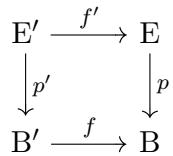
\includegraphics[keepaspectratio]{images/part001_eb35a58e.jpg}}

是一个笛卡尔方块。

事实上，映射 \(h: E' \to B' \times_{B} E\) （由 \(h(x') = (p'(x'), f'(x'))\) 定义的）是主纤维丛的 \(B'\)-态射，因而是同构；此外，我们有 \(pr_{2} \circ h = f'\)，由此得结果 (I, p. 8, prop. 2)。

在前一推论的假设下，有时称 \(f'\) 为主纤维丛的 f-态射。

命题 2. --- 设 (E, p) 为以 B 为基、以 G 为群的主纤维丛，设 \(\varepsilon\) 为截面 \(b \mapsto (b, e)\) （平凡主纤维丛 (B \(\times\) G, \(\mathrm{pr}_{1}\)) 的），其中 \(e\) 表示 G 的单位元。映射 \(h \mapsto h \circ \varepsilon\) 是从 \(\mathcal{C}_{\mathrm{B}}^{\mathrm{G}}(\mathrm{B} \times \mathrm{G}; \mathrm{E})\) 到连续截面所成之集 \(\mathcal{S}(\mathrm{B}; \mathrm{E})\) （\(p\) 的）上的双射。其逆双射把连续截面 \(s\) （\(p\) 的）对应到 B-态射 \((b, g) \mapsto s(b) \cdot g\)。

推论. --- 主纤维丛可平凡化，当且仅当它有连续截面。

命题 3. --- 设 E 与 B 为拓扑空间，\(p\colon\mathrm{E}\to\mathrm{B}\) 为连续映射，G 为右作用于 E 上的拓扑群。下列条件等价：

\begin{enumerate}
\def\labelenumi{(\roman{enumi})}
\item
  赋以映射 p 的 E 是以 B 为基、以 G 为群的主纤维丛；
\item
  对每个 \(x \in E\) 与每个 \(g \in G\) ，有 \(p(x \cdot g) = p(x)\) ，映射 \(\theta: (x, g) \mapsto (x, x \cdot g)\) 是 \(E \times G\) 到 \(E \times_{B} E\) 上的同胚，且 B 的每一点都有邻域，映射 p 在其上存在连续截面。
\end{enumerate}

(i)⇒(ii)：设 (E, p) 是主纤维丛。群 G 连续且自由地作用于 E，其轨道即 p 的纤维。于是映射 \(\theta\) 是双射且连续。更精确地说，若给 \(E \times_{B} E\) 赋以由 \((x, y) \cdot g = (x, y \cdot g)\) 定义的 G 的作用，则映射 \(\theta\) 是平凡主纤维丛 \(E \times G\) 到主纤维丛 \((E \times_{B} E \to E, \mathrm{pr}_{1})\) （例 5）中的 E-态射，因而是同构（命题 1）。(ii) 的其余断言由定义立即得出。

(ii)⇒(i)：令 \(\varphi = pr_{2} \circ \theta^{-1}\) ，于是对每个 \((x, y) \in E \times_{B} E\) ，有

\[
\theta^ {- 1} (x, y) = (x, \varphi (x, y)).\tag{1}
\]

映射 \(\varphi\colon\mathrm{E}\times_{\mathrm{B}}\mathrm{E}\to\mathrm{G}\) 是连续的，且对 \((x,y)\in\mathrm{E}\times_{\mathrm{B}}\mathrm{E}\)，元素 \(\varphi(x,y)\) 是 G 的唯一元素 \(g\) （使得 \(y=x\cdot g\) 的）。设 \(b\) 为 B 的一点；设 U 为 \(b\) 的邻域，\(s\) 为 \(p\) 在 U 上的连续截面。对 \((u,g)\in\mathrm{U}\times\mathrm{G}\)，令 \(f(u,g)=s(u)\cdot g\)；映射 \(f\) 是从 \(U \times G\) 到 \(\overline{p}^{-1}(\mathrm{U})\) 中的 U-态射。对 \(y\in\overline{p}^{-1}(\mathrm{U})\)，令 \(f'(y)=(p(y),\varphi(s(p(y)),y))\)。映射 \(f'\) 是从 \(\overline{p}^{-1}(\mathrm{U})\) 到 U \(\times\) G 中的 U-态射。我们有

\[
(f \circ f ^ {\prime}) (y) = s (p (y)) \cdot \varphi (s (p (y)), y) = y.
\]

另一方面，对 \((u,g)\in \mathrm{U}\times \mathrm{G}\) ，有

\[
(f ^ {\prime} \circ f) (u, g) = f ^ {\prime} (s (u) \cdot g) = (u, \varphi (s (u), s (u) \cdot g)) = (u, g).
\]

因此 f 是 U-同构。由此得出 \((E,p)\) 是以 B 为基、以 G 为群的主纤维丛。

注 1. --- 设 (E, p) 为以 B 为基、以 G 为群的主纤维丛。用命题 3 的记号，映射 \(\theta^{-1}\colon E \times_{B} E \to E \times G\) 是主纤维丛 \(\mathrm{pr}_{1}\colon E \times_{B} E \to E\) 的一个平凡化。称 \(\theta^{-1}\) 为这个主纤维丛的典范平凡化。

推论 1. --- 设 G 为连续右作用于拓扑空间 E 上的拓扑群。下列条件等价：

\begin{enumerate}
\def\labelenumi{(\roman{enumi})}
\item
  轨道空间 E/G 是 Hausdorff 的，且赋以典范映射 \(p: E \rightarrow E/G\) 的空间 E 是以 G 为群的主纤维丛；
\item
  群 G 逆紧地 (TG, III, p. 27) 且自由地作用于 E，且 E/G 的每一点都有邻域，映射 p 在其上存在连续截面。
\end{enumerate}

令 \(B=E/G\)。在假设 (i) 与 (ii) 的每一个之下，群 G 都连续且自由地作用于 E，于是映射 \(\theta\colon(x,g)\mapsto(x,x\cdot g)\) 是从 \(E\times G\) 到 \(E\times_{B}E\) 上的连续双射。我们置于这个假设之下，并用 \(\varphi\colon E\times_{B}E\to G\) 表示映射 \(pr_{2}\circ\theta^{-1}\)。顾及公式 (1)，\(\theta\) 是同胚，当且仅当映射 \(\varphi\) 是连续的。另一方面，由于 G 所定义的等价关系是开的 (TG, III, p. 10, lemma 2)，空间 E/G 是 Hausdorff 的，当且仅当这个等价关系的图 \(E\times_{B}E\) 在 \(E\times E\) 中是闭的。G 逆紧地作用于 E，当且仅当 \(E\times_{B}E\) 在 \(E\times E\) 中是闭的且映射 \(\varphi\) 是连续的。于是条件 (i) 与 (ii) 的等价性由命题 3 得出。

推论 2. --- 设 G 为拓扑群，H 为 G 的子群，p: G → G/H 为典范映射。若映射 p 在 G/H 的某个非空开集上有连续截面，则 p 使 G 成为以 G/H 为基、以 H 为群的主纤维丛。

通过左平移，G/H 的每一点都有邻域，映射 p 在其上有连续截面。另一方面，对 \((g,g')\) （属于 \(G\times G\) 的），令 \(\varphi(g,g')=g^{-1}g'\)。若 \(p(g)=p(g')\)，则 \(\varphi(g,g')\) 属于 H。映射 \((g,g')\mapsto(g,\varphi(g,g'))\) （从 \(G\times_{G/H}G\) 到 \(G\times H\) 的）是连续的，且是连续映射 \(\theta: G\times H\to G\times_{G/H}G\) （由 \(\theta(g,h)=(g,gh)\) 定义的）的逆，由此得该推论。

注 2. --- 这种情形特别出现于：G 是实李群，有限维、无穷可数，解析地且可迁地作用于解析流形 X。若取 H 为 X 的某点的稳定子，则映射 p 是 G 到齐性李空间 G/H 上的浸没，后者同构于 X (LIE, III, p. 109, corollary)。因此它有局部截面 (VAR, p. 50)。

\subsection{主覆叠}

定义 2. —— 设 B 为拓扑空间，G 为群。给 G 赋予离散拓扑。以 B 为基、以 G 为群的主纤维丛称为 B 的以 G 为群的主覆叠。

这一术语是合理的，因为这样的 B-空间是 B 的一个覆叠。

非空拓扑空间上的主 G-丛具有次数，等于 Card G。

命题 4. —— 设 B 为拓扑空间，(E, p) 为 B-空间，G 为从右边作用于 E 的离散拓扑群。下列断言等价：

\begin{enumerate}
\def\labelenumi{(\roman{enumi})}
\item
  B-空间 E 是以 G 为群的主覆叠；
\item
  对每个 \(g \in G\) 和每个 \(x \in E\) ，有 \(p(x \cdot g) = p(x)\) ，映射 p 诱导从 E/G 到 B 上的同胚，且映射 \(\theta: (x, g) \mapsto (x, x \cdot g)\) 是从 E × G 到 \(E \times_{B} E\) 上的同胚；
\item
  群 G 连续且自由地作用于 E，映射 p 是平展的，且其纤维是 G 的轨道。
\end{enumerate}

(i)⇒(ii)：这由 I, 第 91 页以及 I, 第 94 页命题 3 得出。(ii)⇒(iii)：在假设 (ii) 之下，G 的作用法则是连续的，且映射 p 是满射且开映射（TG, III, 第 10 页, 引理 2）。设 \(x \in E\) ；映射 \(\theta\) 诱导从 \(\{x\} \times G\) 到 \(\{x\} \times p^{-1}(p(x))\) 上的双射，故群 G 自由作用，且其轨道是 p 的纤维。若以 e 表示 G 的单位元，则 \(E \times_{B} E\) 的对角线是 \(E \times \{e\}\) 在同胚 \(\theta\) 下的像。由于群 G 是离散的，集合 \(\{e\}\) 在 G 中是开集，从而对角线 \(\Delta_{E}\) 在 \(E \times_{B} E\) 中是开集。由 I, 第 31 页命题 7，映射 p 是平展的。

(iii)⇒(i)：由于 p 的每个纤维都是 G 在 E 上作用的一条轨道，映射 p 是满射。因为 p 是平展的，对 B 的每个点 b，存在 b 的开邻域 U 以及 p 在 U 上的连续截面 s。集合 \(s(\mathrm{U})\) 在 E 中是开集，且 s 诱导从 U 到 \(s(\mathrm{U})\) 上的同胚（I, 第 30 页, 推论 3）。对每个 \(g \in G\)，集合 \(s(\mathrm{U}) \cdot g\) 在 E 中是开集，且这些集合对一切 \(g \in G\) 的并等于 \(p^{-1}(\mathrm{U})\)。若 g 与 \(g'\) 是 G 的两个不同元素，则集合 \(s(\mathrm{U}) \cdot g\) 与 \(s(\mathrm{U}) \cdot g'\) 不相交，因为 G 自由地作用于 E。映射 \(f: U \times G \to p^{-1}(\mathrm{U})\) 由 \(f(u, g) = s(u) \cdot g\) 所定义，对 \((u, g) \in U \times G\) 是连续的，因而是从 \(U \times G\) 到 \(p^{-1}(\mathrm{U})\) 上的与 G 的右作用相容的同胚。按定义，E 因而是 B 的以 G 为群的主覆叠。

例. —— 1) 设 E 为拓扑空间，G 为从右边连续且自由地作用于 E 的离散拓扑群。为使典范映射 \(p \colon \mathrm{E} \to \mathrm{E} / \mathrm{G}\) 使 E 成为 E/G 的主覆叠，充要条件是该映射是平展的（命题 4 的条件 (iii)）。例如，假设存在拓扑空间 X 以及与 G 在 E 上的作用相容的平展映射 \(q \colon \mathrm{E} \to \mathrm{X}\) ；则 E 是 E/G 的主覆叠。事实上，以 \(q' \colon \mathrm{E} / \mathrm{G} \to \mathrm{X}\) 表示由 \(q\) 诱导的映射；我们有 \(q = q' \circ p\)，因此由 I, 第 29 页命题 6 d)，\(p\) 是平展的。

\begin{enumerate}
\def\labelenumi{\arabic{enumi})}
\setcounter{enumi}{1}
\tightlist
\item
  设 \(q \colon \mathrm{E} \to \mathrm{X}\) 为分离平展态射。群 \(\operatorname{Aut}_{\mathrm{X}}(\mathrm{E})\) 赋予离散拓扑后，从左边连续地作用于 E。若空间 E 连通，则此作用是自由的（I, 第 34 页, 推论 2）。以 G 表示群 \(\operatorname{Aut}_{\mathrm{X}}(\mathrm{E})^{\circ}\) ，并给 E 赋予与 \(\operatorname{Aut}_{\mathrm{X}}(\mathrm{E})\) 的作用相反的右作用。由前例，赋予典范映射 \(p \colon \mathrm{E} \to \mathrm{E} / \mathrm{G}\) 的空间 E 是以 G 为群的主覆叠。
\end{enumerate}

\subsection{离散群的逆紧且自由的作用}

定理 1. —— 设 G 为从右边连续作用于拓扑空间 E 的离散群。假设 E 的每个点都有邻域 U，使得对 G 的每个异于单位元的元素 g，有 U ∩ (U · g) = ∅。则典范映射 p: E → E/G 使 E 成为 E/G 的以 G 为群的主覆叠。

依假设，G 在 E 上的作用是自由的，故只需证明映射 p 是平展的（I, 第 98 页, 例 1）。设 x 为 E 的点，U 为 x 的开邻域，使得对 G 的每个异于单位元的元素 g 有 \(U \cap U \cdot g = \varnothing\) 。映射 p 是开的（TG, III, 第 10 页, 引理 2），且诱导从 U 到 \(p(\mathrm{U})\) 的单射、连续且开的映射，因而是同胚，这就证明了映射 p 是平展的。

例. —— 1) 设 n 为整数 \(\geqslant 0\) ，\(\mathbf{P}_{n}(\mathbf{R})\) 为 n 维射影空间（TG, VI, 第 13 页），\(S_{n}\) 为 \(R^{n+1}\) 中的单位球面（TG, VI, 第 9 页）。从 \(S_{n}\) 到 \(\mathbf{P}_{n}(\mathbf{R})\) 上的典范映射使 \(S_{n}\) 成为以 \(\{1,-1\}\) 为群的主覆叠，该群以位似作用；轨道是由直径上相对的点组成的偶。

\begin{enumerate}
\def\labelenumi{\arabic{enumi})}
\setcounter{enumi}{1}
\item
  每个次数为 2 的覆叠都具有唯一的以 Z/2Z 为群的主覆叠结构。
\item
  设 X 为 R 上有限维的局部分离微分流形，\(\widetilde{X}\) 为 X 的切丛的定向流形（VAR, R, 10.2.4）。空间 \(\widetilde{X}\) 连同它到 X 上的典范投影，是以 \(\{1,-1\}\) 为群的 X 的主覆叠。
\end{enumerate}

推论 1. —— 设 G 为从右边连续作用于拓扑空间 E 的离散拓扑群。下列条件等价：

\begin{enumerate}
\def\labelenumi{(\roman{enumi})}
\item
  群 G 逆紧且自由地作用于 E；
\item
  空间 E/G 是豪斯多夫的，且 E 是以 E/G 为基、以 G 为群的主覆叠。
\end{enumerate}

此外，在这些条件之下，空间 E 是豪斯多夫的。

设条件 (i) 成立。则空间 E 与 E/G 都是分离的（TG, III, 第 29 页, 命题 3），且对每个 \(x \in \mathrm{E}\) ，存在 \(x\) 在 E 中的开邻域 U，使得 \(\mathrm{U} \cap (\mathrm{U} \cdot g) = \varnothing\) 对 G 的每个异于单位元的元素 \(g\) 成立（TG, III, 第 32 页, 命题 8）。由定理 1，条件 (ii) 随之成立。

蕴涵 (ii)⇒(i) 由 I, 第 96 页推论 1 得出。

推论 2. —— 设 G 为拓扑群，H 为 G 的离散子群。让 H 以右平移作用于 G。则从 G 到模 H 的左陪集空间 G/H 中的典范映射赋予 G 一个 G/H 的以 H 为群的主覆叠结构。

设 V 为 G 的单位元 \(e\) 的邻域，使得 \(\mathrm{H} \cap \mathrm{V} = \{e\}\) 。存在 \(e\) 在 G 中的开邻域 U，使得 \(\mathrm{U}^{-1} \cdot \mathrm{U} \subset \mathrm{V}\) （TG, III, 第 3 页），从而 \(\mathrm{U} \cap \mathrm{U} \cdot h = \varnothing\) 对所有 \(h \in \mathrm{H}\) （\(h \neq e\) ）成立。因此，I, 第 100 页的推论 2 由定理 1 得出。

例 4. —— 赋予从 R 到 T = R/Z 的典范映射（TG, V, 第 2 页），R 是 R/Z 的以 Z 为群的主覆叠。

注 1. —— 设 G 为分离拓扑群，K 为 G 的紧子群，H 为 G 的离散子群。群 G 从右边连续且逆紧地作用于模 K 的右陪集空间 K\G（TG, III, 第 30 页, 推论）。由于子群 H 在 G 中是闭的，它也逆紧地作用于 K\G（TG, III, 第 27 页, 例 1）。此外，若 \(H \cap gKg^{-1} = \{e\}\) 对所有 \(g \in G\) 成立，则群 H 自由地作用于 K\G。于是由推论 1，空间 K\G 是 K\G/H 的以 H 为群的主覆叠。

推论 3. —— 设 G 与 G' 为拓扑群，\(\varphi\colon G \to G'\) 为连续、开且满的同态。假设 \(\varphi\) 的核 H 是离散的。则对于 H 以右平移在 G 上的作用，\(\varphi\) 使 G 成为 G' 的以 H 为群的主覆叠。

此外，若群 G 连通，则 H 包含于 G 的中心。

同态 \(\varphi\) 诱导从 G/H 到 G' 上的拓扑群同构（TG, III, 第 16 页, 命题 24），由此并利用推论 2 即得第一个断言。设群 G 连通。对每个 \(h \in \mathrm{H}\) ，由 \(g \mapsto ghg^{-1}\) 定义的从 G 到 H 的连续映射是常值的，取值为 \(h\) 。故群 H 包含于 G 的中心。

注. —— 2) 设 G 与 G' 为拓扑群，\(\varphi\colon\mathrm{G}\to\mathrm{G}'\) 为连续且开的同态。若群 G' 连通，则同态 \(\varphi\) 是满射。事实上，\(\varphi(\mathrm{G})\) 是 \(\mathrm{G}'\) 的开子群，从而是闭子群，于是等于 \(\mathrm{G}'\)。

\begin{enumerate}
\def\labelenumi{\arabic{enumi})}
\setcounter{enumi}{2}
\tightlist
\item
  设 G 为无穷可数的局部紧群，G' 为基础空间为贝尔空间的分离拓扑群。每个从 G 到 G' 上的连续满同态都是开的（TG, IX, 第 56 页, 推论及 TG, III, 第 16 页, 命题 24）。
\end{enumerate}

例. —— 5) 对每个整数 \(n > 0\)，以 \(\mu_{n}\) 表示 C 中 n 次单位根组成的群（A, V, 第 75 页）。映射 \(z \mapsto z^{n}\) 使 \(C^{*}\) 成为 \(C^{*}\) 的以 \(\mu_{n}\) 为群的主覆叠，该群在 \(C^{*}\) 中以乘法作用。

\begin{enumerate}
\def\labelenumi{\arabic{enumi})}
\setcounter{enumi}{5}
\tightlist
\item
  赋予映射 \(z \mapsto e^{2\pi iz}\) （TG, VIII, 第 8 页, 注），空间 C 是 \(C^{*}\) 的以 Z 为群的主覆叠。映射 \(x \mapsto e^{2\pi ix} = \mathbf{e}(x)\) （从 R 到 \(S_{1}\) ）使 R 成为 \(S_{1}\) 的以 Z 为群的主覆叠。
\end{enumerate}

\subsection{伽罗瓦覆叠}

定义 3. —— 设 B 为非空拓扑空间。称 B 的覆叠 E 为伽罗瓦覆叠，如果它是连通的，且对 B 的每个点 b，由 E 的 B-自同构组成的群 \(\mathrm{Aut}_{B}(E)\) 在纤维 \(E_{b}\) 上的作用是传递的。

设 E 为拓扑空间 B 的伽罗瓦覆叠，p 为其投影。映射 p 是满射（A, I, 第 56 页, 定义 6），故空间 B 是连通的。因而覆叠 (E, p) 具有次数，且该次数非零。

命题 5. —— 设 B 为非空拓扑空间，E 为 B 的伽罗瓦覆叠。映射 \((h,x)\mapsto h(x)\) （从 \(\mathrm{Aut}_{\mathrm{B}}(\mathrm{E})\times\mathrm{E}\) 到 E 中）是群 \(\mathrm{Aut}_{\mathrm{B}}(\mathrm{E})^{\circ}\) 在 E 上的一个右作用，它使 E 成为以 \(\mathrm{Aut}_{\mathrm{B}}(\mathrm{E})^{\circ}\) 为群的主覆叠。

给群 \(\mathrm{Aut}_{\mathrm{B}}(\mathrm{E})^{\circ}\) 赋予离散拓扑；此时运算法则 \((h,x)\mapsto h(x)\) 是连续的。此作用是自由的（I, 第 34 页, 命题 11 的推论 2）。由于 E 是 B 的伽罗瓦覆叠，其纤维都是该作用的轨道。由 I, 第 97 页命题 4，E 是以 \(\mathrm{Aut}_{\mathrm{B}}(\mathrm{E})^{\circ}\) 为群的主覆叠。

定理 2. —— 设 B 为连通拓扑空间，E 为 B 的连通非空覆叠。下列性质等价：

\begin{enumerate}
\def\labelenumi{(\roman{enumi})}
\item
  覆叠 E 是伽罗瓦的。
\item
  存在离散拓扑群 G 以及 G 在 E 上的连续右作用，使 E 成为以 G 为群的主覆叠。
\item
  E 的覆叠 \(E \times_{B} E\) （由投影 \(\mathrm{pr}_{1}\) 所定义）是可平凡化的。
\end{enumerate}

当这些条件成立时，由 G 的作用所定义的典范映射 \(G \to \mathrm{Aut}_{B}(E)^{\circ}\) 是群同构。

此外，若空间 B 是局部连通的，则上述性质等价于下述性质：

(i') 存在 B 的点 b，使得群 \(\mathrm{Aut}_{\mathrm{B}}(\mathrm{E})\) 在纤维 \(E_{b}\) 上的作用是传递的。

蕴涵 (i)⇒(ii) 由命题 5 得出，蕴涵 (ii)⇒(iii) 由 I, 第 95 页注 1 得出。我们来证明 (iii)⇒(i)。以 \(p\colon E \to B\) 表示覆叠 E 的投影。由于 B 连通，该覆叠具有次数，又因 E 非空，此次数非零。设 \(b\) 为 B 的一点。我们来证明 \(\mathrm{Aut}_{B}(E)\) 在纤维 \(E_{b}\) 上的作用是传递的。由前所述，该纤维非空。设 \(x\) 与 \(x'\) 为 \(E_{b}\) 中的点。B-态射 \(h\colon E \to E\) （满足 \(h(x) = x'\) ）与连续截面 \(s\) 成一一对应，后者是映射 \(\mathrm{pr}_{1}\colon E \times_{B} E \to E\) 的截面，且满足 \(s(x) = (x, x')\) （I, 第 9 页, 命题 3）。在假设 (iii) 之下，这样的截面存在（I, 第 70 页, 推论 2），且因空间 E 连通而是唯一的（I, 第 34 页, 命题 11 的推论 1）。于是，对每个偶 \((x, x') \in E \times_{B} E\)，存在唯一的 B-态射 \(h\colon E \to E\) 使得 \(h(x) = x'\) 。若 \(h'\colon E \to E\) 是满足 \(h'(x') = x\) 的唯一 B-态射，则有 \(h'(h(x)) = x\) 与 \(h(h'(x')) = x'\) ，从而 \(h' \circ h = \text{Id}_E\) 且 \(h \circ h' = \text{Id}_E\) 。这就证明 \(h\) 是 E 的 B-自同构。因而覆叠 E 是伽罗瓦的。

我们已证明条件 (i)、(ii)、(iii) 等价。设它们成立。以 \(\delta\colon\mathbf{G}\to\mathrm{Aut}_{\mathrm{B}}(\mathrm{E})\) 表示把 \(g\in\mathrm{G}\) 对应到 E 的 B-自同构 \(x\mapsto x\cdot g\) 的映射。映射 \(\delta\) 是从 G 到 \(\mathrm{Aut}_{\mathrm{B}}(\mathrm{E})^{\circ}\) 中的群同态。由于 G 自由地作用于 E，映射 \(\delta\) 是单射。设 \(h\in\mathrm{Aut}_{\mathrm{B}}(\mathrm{E})\)，\(x\in\mathrm{E}\) ，并设 \(g\) 为 G 中满足 \(x\cdot g=h(x)\) 的唯一元素。

B-态射 \(h\) 与 \(\delta(g)\) 在点 \(x\) 处取值相同，从而由于空间 E 连通而处处相同（I, 第 34 页, 命题 11 的推论 1），这就证明了 \(\delta\) 是同构。

现在设空间 B 局部连通，我们证明在假设 (i') 之下覆叠 E 是伽罗瓦的。设 \(E'\) 为 E 按群 \(\mathrm{Aut}_{B}(E)^{\circ}\) 的右作用所得的商空间，并以 \(q\colon E \to E'\) 表示典范映射。它使 E 成为 E' 的满覆叠（I, 第 98 页, 例 2）；映射 \(p\colon E \to B\) 过渡到商，定义出连续映射 \(p'\colon E' \to B\) ，满足 \(p'\circ q = p\) 。由于空间 B 局部连通，B-空间 \((E', p')\) 是一个覆叠（I, 第 81 页, 命题 7）。在假设 (i') 之下，存在 B 的点 \(b\) 使得纤维 \(E'_{b}\) 恰有一个元素；由于空间 B 连通，对 B 的每个点 \(b\) 同样成立（I, 第 74 页, 命题 4），这就证明了 E 是 B 的伽罗瓦覆叠。

命题 6. —— 设 B 为拓扑空间，G 为群。设 (E, p) 为 B 的以 G 为群的主覆叠。假设空间 B 连通且局部连通。设 E₀ 为 E 的一个连通分支，G₀ 为 G 中稳定 E₀ 的子群（A, I, 第 51 页）。B-空间 (E₀, p \textbar{} E₀) 对于 G₀ 在 E₀ 上的右动作是一个主覆叠。此覆叠是伽罗瓦的。

由于空间 B 局部连通，E 亦然，故 \(E_{0}\) 是 E 的开子空间（TG, I, 第 85 页, 命题 11）。又因它还是闭的（TG, I, 第 83 页），空间 \(E_{0}\) 因而是 B 的覆叠（I, 第 80 页, 推论 1）。由于 B 连通，该覆叠具有次数；由于 \(E_{0}\) 非空，\(p|E_{0}\) 的一切纤维都非空。设 x 为 \(E_{0}\) 的一点，并设 \(x' \in E_{0}\) 满足 \(p(x') = p(x)\)；存在元素 \(g \in G\) 使得 \(x \cdot g = x'\)。由于连通分支 \(E_{0}\) 与 \(E_{0} \cdot g\) 有公共点，二者相等，由此得 \(g \in G_{0}\)。于是，群 \(G_{0}\) 传递地作用于 B-空间 \(E_{0}\) 在 \(p(x)\) 处的纤维上。命题 6 得证。

注记. —— 若在命题 6 中不假设空间 B 局部连通，则空间 \(E_{0}\) 可能不是 B 的覆叠（I, 第 147 页, 习题 1）。

\subsection{相伴纤维丛}

设 E 与 F 为集合，G 为作用于 E 的右边、作用于 F 的左边的群。群 G 作用于乘积 \(E \times F\) 的右边，其法则为 \((x, y) \cdot g = (x \cdot g, g^{-1} \cdot y)\) ，其中 \(g \in G\)，\((x, y) \in E \times F\) 。 \(E \times F\) 对此作用的商集记作 \(E \times^{G} F\) 。

当 E 与 F 是拓扑空间时，给集合 \(E \times^{G} F\) 赋予由 \(E \times F\) 的拓扑诱导的商拓扑。从 \(E \times F\) 到 \(E \times^{G} F\) 上的典范映射是连续的。若群 G 连续地作用于 E 与 F，则它是开的。

另外，设 \(F'\) 为 G 从左边作用于其上的集合，\(h: F \to F'\) 为与 G 在 F 与 \(F'\) 上的作用相容的映射（A, I, 第 50 页）。映射 \(Id_{E} \times h: E \times F \to E \times F'\) 与 G 的作用相容，并且通过过渡到商，定义一个记作 \(Id_{E} \times^{G} h\) 的、从 \(E \times^{G} F\) 到 \(E \times^{G} F'\) 中的映射。

若 \(h \colon F \to F'\) 是连续映射（与 G 在 F 与 \(F'\) 上的作用相容），则映射 \(\mathrm{Id}_{\mathrm{E}} \times^{\mathrm{G}} h\) 是连续的（TG, I, 第 21 页, 命题 6）。

例. —— 1) 设 F 为拓扑空间，G 为从左边连续作用于 F 的拓扑群。若给拓扑空间 G 赋予 G 以右平移的作用，则空间 G × \(^{G}\) F 典范地等同于 F，如下所述。连续映射 \(\varphi\) : F → G × F 与 \(\psi\) : G × F → F （分别由 \(\varphi(f) = (e, f)\) （其中 e 表示 G 的单位元）与 \(\psi(g, f) = g \cdot f\) 定义）诱导出连续映射 \(\overline{\varphi}\) : F → G × \(^{G}\) F 与 \(\overline{\psi}\) : G × \(^{G}\) F → F，二者互为逆映射。

\begin{enumerate}
\def\labelenumi{\arabic{enumi})}
\setcounter{enumi}{1}
\item
  例 1 可如下推广。设 B 与 F 为拓扑空间，G 为从左边连续作用于 F 的拓扑群。通过过渡到商，由 (b, f) ↦ ((b, e), f) 给出的从 B × F 到 (B × G) × F 的映射，以及由 ((b, g), f) ↦ (b, gf) 给出的从 (B × G) × F 到 B × F 的映射，定义出互为逆映射的 B-同构 B × F → (B × G) × \(^{G}\) F 与 (B × G) × \(^{G}\) F → B × F。
\item
  类似地，设 E 为拓扑空间，G 为从右边连续作用于 E 的拓扑群。若给拓扑空间 G 赋予 G 以左平移的作用，则空间 \(E \times^{G} G\) 等同于 E。
\end{enumerate}

设 E 与 F 为拓扑空间，G 为从右边连续作用于 E、从左边连续作用于 F 的拓扑群。设 B 为拓扑空间，\(p\colon E \to B\) 为满足 \(p(x \cdot g) = p(x)\) （其中 \(x \in E\)，\(g \in G\)）的连续映射。映射 \(p \circ pr_{1}\colon E \times F \to B\) 通过过渡到商，定义一个连续映射 \(p^{F}\colon E \times^{G} F \to B\) ，而典范映射 \(\pi\colon E \times F \to E \times^{G} F\) 是一个 B-态射。

设 B' 为拓扑空间，\(h\colon B'\to B\) 为连续映射。群 G 连续地作用于 \(B'\times_{B}E\) 的右边，其作用法则为 \(((b',x),g)\mapsto(b',x\cdot g)\)。将典范同构 \(((b',x),y)\mapsto(b',(x,y))\) ——它把 \((\mathrm{B}'\times_{\mathrm{B}}\mathrm{E})\times\mathrm{F}\) 映到 \(\mathrm{B}'\times_{\mathrm{B}}(\mathrm{E}\times\mathrm{F})\) 上——与映射 \(\operatorname{Id}_{\mathrm{B}'}\times\pi\) （从 \(\mathrm{B}'\times_{\mathrm{B}}(\mathrm{E}\times\mathrm{F})\) 到 \(\mathrm{B}'\times_{\mathrm{B}}(\mathrm{E}\times^{\mathrm{G}}\mathrm{F})\) 中）复合，得到连续映射 \(\lambda_{0}\colon(\mathrm{B}'\times_{\mathrm{B}}\mathrm{E})\times\mathrm{F}\to\mathrm{B}'\times_{\mathrm{B}}(\mathrm{E}\times^{\mathrm{G}}\mathrm{F})\)。它通过过渡到商，定义一个连续映射

\[
\lambda \colon (\mathrm{B} ^ {\prime} \times_ {\mathrm{B}} \mathrm{E}) \times^ {\mathrm{G}} \mathrm{F} \rightarrow \mathrm{B} ^ {\prime} \times_ {\mathrm{B}} (\mathrm{E} \times^ {\mathrm{G}} \mathrm{F}).
\]

引理. —— 映射 λ 是同胚。

映射 \(\lambda_0\) 是满射，且 \((\mathrm{B}' \times_{\mathrm{B}} \mathrm{E}) \times \mathrm{F}\) 中两个元素在 \(\lambda_0\) 下有同一像，当且仅当它们属于 G 在 \((\mathrm{B}' \times_{\mathrm{B}} \mathrm{E}) \times \mathrm{F}\) 上作用的同一轨道。由此可知映射 \(\lambda\) 是双射。由于映射 \(\pi\) 是开的，映射 \(\mathrm{Id}_{\mathrm{B}'} \times_{\mathrm{B}} \pi\) 也是开的（I, 第 17 页, 命题 8），从而 \(\lambda_0\) 与 \(\lambda\) 也是开的（TG, I, 第 32 页, 命题 3），这就证明了 \(\lambda\) 是同胚。

命题 7. —— 设 B 为拓扑空间，G 为拓扑群，(E,p) 为 B 上以 G 为群的主纤维丛，F 为 G 从左边连续作用于其上的拓扑空间。

\begin{enumerate}
\def\labelenumi{\alph{enumi})}
\item
  拓扑空间 \(E \times^{G} F\) 连同连续映射 \(p^{F}: E \times^{G} F \to B\) （由映射 \(p \circ pr_{1}: E \times F \to B\) 过渡到商而得），是以 F 为纤维型的局部平凡纤维丛；若 B-丛 E 可平凡化，则它也可平凡化。
\item
  设 \(\pi\colon\mathrm{E}\times\mathrm{F}\to\mathrm{E}\times^{\mathrm{G}}\mathrm{F}\) 为典范满射。映射 \(\mu\colon\mathrm{E}\times\mathrm{F}\to\mathrm{E}\times_{\mathrm{B}}(\mathrm{E}\times^{\mathrm{G}}\mathrm{F})\) 使 \((x,\pi(x,f))\) 对应于 \((x,f)\) ，它是一个同胚，其逆映射是 E 上的局部平凡纤维丛 \((\mathrm{E}\times_{\mathrm{B}}(\mathrm{E}\times^{\mathrm{G}}\mathrm{F}),\mathrm{pr}_{1})\) 的一个平凡化。
\end{enumerate}

先设 E 为平凡主纤维丛 \(B \times G\) 。由例 2，此时空间 \(E \times^{G} F\) 等同于 \(B \times F\) ，映射 \(p^{F}\) 等同于第一投影 \(pr_{1}: B \times F \to B\) ，这就证明在此情形 \((\mathrm{E} \times^{\mathrm{G}}\mathrm{F}, p^{\mathrm{F}})\) 是 B 上的可平凡化纤维丛。在一般情形，B 的每个点都有邻域 U，使映射 \(p_{\mathrm{U}}: p^{-1}(\mathrm{U}) \to \mathrm{U}\) 把 \(p^{-1}(\mathrm{U})\) 变为 U 上的可平凡化主纤维丛。由前所述，\((p^{-1}(\mathrm{U}) \times^{\mathrm{G}}\mathrm{F} \to \mathrm{U}, (p_{\mathrm{U}})^{\mathrm{F}})\) 是 U 上的可平凡化纤维丛。把上面的引理应用于 \(B' = U\) 且 \(h: U \to B\) 为典范单射的情形，对 U-空间 \(((p^{\mathrm{F}})^{-1}(\mathrm{U}), (p^{\mathrm{F}})_{\mathrm{U}})\) （由 \((\mathrm{E} \times^{\mathrm{G}}\mathrm{F}, p^{\mathrm{F}})\) 限制到 U 上得到）结论同样成立。这就证明 \((\mathrm{E} \times^{\mathrm{G}}\mathrm{F}, p^{\mathrm{F}})\) 是 B 上的局部平凡纤维丛，从而完成了断言 a) 的证明。

映射 \(\theta\colon\mathrm{E}\times\mathrm{G}\to\mathrm{E}\times_{\mathrm{B}}\mathrm{E}\) 由 \(\theta(x,g)=(x,x\cdot g)\) 所定义，它是同胚（I, 第 94 页, 命题 3），且与 G 在 E \(\times\) G 上和 E \(\times_{\mathrm{B}}\) E 上由 \(((x,g),g')\mapsto(x,gg')\) 与 \(((x,y),g')\mapsto(x,yg')\) 给出的作用相容。因此 \(\theta\) 通过过渡到商，诱导出同胚 \(\theta'\) （从 (E \(\times\) G) \(\times^{\mathrm{G}}\) F 到 (E \(\times_{\mathrm{B}}\) E) \(\times^{\mathrm{G}}\) F 上）。映射 \(\mu\) 是同胚 E \(\times\) F \(\rightarrow\) (E \(\times\) G) \(\times^{\mathrm{G}}\) F （例 2）、\(\theta'\) 以及典范同胚 (E \(\times_{\mathrm{B}}\) E) \(\times^{\mathrm{G}}\) F \(\rightarrow\) E \(\times_{\mathrm{B}}\) (E \(\times^{\mathrm{G}}\) F) （I, 第 105 页, 引理）的复合，由此即得 \(b\) 。

在命题 7 的假设之下，局部平凡纤维丛 (E × \(^{G}\) F, p \(^{F}\) ) 称为与主纤维丛 (E, p) 相伴的、以 F 为纤维型的局部平凡纤维丛。B-空间 E × \(^{G}\) F 的一切纤维都与空间 F 同胚。特别地，若空间 F 是离散的，则映射 p \(^{F}\) 是一个覆叠。

例. —— 4) 设 B 为拓扑空间，G 为拓扑群，(E, p) 为 B 上的主 G-丛。设 H 为 G 的子群。

以 \(\varphi\colon\mathrm{E}\to\mathrm{E}\times(\mathrm{G}/\mathrm{H})\) 与 \(\psi\colon\mathrm{E}\times(\mathrm{G}/\mathrm{H})\to\mathrm{E}/\mathrm{H}\) 表示由 \(\varphi(x)=(x,\mathrm{H})\) 与 \(\psi(x,g\mathrm{H})=(x\cdot g)\mathrm{H}\) 定义的映射。它们与到 B 的投影以及 G 的作用相容，并通过过渡到商，定义出互为逆映射的 B-空间态射 \(\overline{\varphi}\colon\mathrm{E}/\mathrm{H}\to\mathrm{E}\times^{\mathrm{G}}(\mathrm{G}/\mathrm{H})\) 与 \(\overline{\psi}\colon\mathrm{E}\times^{\mathrm{G}}(\mathrm{G}/\mathrm{H})\to\mathrm{E}/\mathrm{H}\) 。我们称 \(\overline{\varphi}\) 为从 E/H 到 \(\mathrm{E}\times^{\mathrm{G}}(\mathrm{G}/\mathrm{H})\) 上的典范同胚。特别地，拓扑空间 E/H 连同连续映射 \(p_{\mathrm{H}}\colon\mathrm{E}/\mathrm{H}\to\mathrm{B}\) ，是 B 上的以 G/H 为纤维型的局部平凡纤维丛。

此外，若 H 是 G 的正规子群，则 G 的作用通过过渡到商，赋予 B-空间 E/H 一个以 G/H 为群的主纤维丛结构。

特别地，若 E 是 B 的以 G 为群的主覆叠，则 E/H 是 B 的覆叠；若 H 在 G 中正规，则它是以 G/H 为群的主覆叠。

\begin{enumerate}
\def\labelenumi{\arabic{enumi})}
\setcounter{enumi}{4}
\item
  设 B 为拓扑空间，G 为拓扑群，E 为 B 上的主 G-丛。设 F 为关于 G 的拓扑齐性空间（TG, III, 第 12 页）。设 y 为 F 的一点，\(G_{y}\) 为其稳定子。映射 \(\varphi_{y}\colon x\mapsto(x,y)\) （从 E 到 \(E\times F\)）通过过渡到商，定义出同胚 \(\overline{\varphi}_{y}\) （从 \(E/G_{y}\) 到 \(E\times^{G}F\) 上）。当群 G 交换时，子群 \(G_{y}\) 不依赖于点 y，但同胚 \(\overline{\varphi}_{y}\) 一般依赖于它。
\item
  设 B 为拓扑空间，G 为拓扑群，\((E,p)\) 为 B 上的主 G-丛。设 H 为拓扑群，\(f:G\to H\) 为拓扑群态射；给 H 赋予由 \(g\cdot h=f(g)h\) 给出的 G 的左作用。
\end{enumerate}

设 \(q \colon \mathrm{E} \times \mathrm{H} \to \mathrm{E} \times^{\mathrm{G}} \mathrm{H}\) 为典范映射；它是开的，从而是普遍严格的（I, 第 20 页, 推论 11）。映射 \(m \colon (x, h, h') \mapsto q(x, hh')\) （从 \(\mathrm{E} \times \mathrm{H} \times \mathrm{H}\) 到 \(\mathrm{E} \times^{\mathrm{G}} \mathrm{H}\) 中）是连续的。设 \((x, h) \in \mathrm{E} \times \mathrm{H}\) ，\(h' \in \mathrm{H}\) 以及 \(g \in \mathrm{G}\) ；我们有 \(m(xg, f(g)^{-1}h, h') = q(xg, f(g)^{-1}hh') = q(x, hh') = m(x, h, h')\) 。因此，存在唯一的映射

\[
m ^ {\prime} \colon (\mathrm{E} \times^ {\mathrm{G}} \mathrm{H}) \times \mathrm{H} \rightarrow \mathrm{E} \times^ {\mathrm{G}} \mathrm{H}
\]

使得 \(m'(q(x,h),h') = q(x,hh')\) 对一切 \(x \in E\) 与一切 \(h, h' \in H\) 成立。由于 q 是普遍严格的，映射 \(m'\) 是连续的。这是拓扑群 H 在 B-空间 \(E \times^{G} H\) 上的一个右作用。

设 U 为 B 的开子集，使得 \(E_{U}\) 同构于 U 上的主纤维丛 \(U \times G\) 。赋予 H 的作用后，U-空间 \((\mathrm{E} \times^{\mathrm{G}}\mathrm{H})_{\mathrm{U}}\) 等同于主纤维丛 \(U \times H\) 。这就证明 \(E \times^{G}H\) 是 B 上的主 H-丛。

定义 4. —— 设 B 为拓扑空间，G 为拓扑群。称 B 上的局部平凡纤维丛 X 与 B 上以 G 为群的主纤维丛 E 相伴，如果存在一个 G 从左边连续作用于其上的拓扑空间 F，以及一个从 E × \(^{G}\) F 到 X 上的 B-同构。

设 E 为 B 上的主 G-丛，X 为 B 上与 E 相伴的局部平凡纤维丛。若主丛 E 可平凡化，则 X 可平凡化（命题 7）。若 B' 为拓扑空间且 \(h \colon \mathrm{B}' \to \mathrm{B}\) 为连续映射，则由 X 经换基得到的局部平凡纤维丛 \(\mathrm{B}' \times_{\mathrm{B}} \mathrm{X}\) 与 B' 上的主纤维丛 \(\mathrm{B}' \times_{\mathrm{B}} \mathrm{E}\) 相伴（I, 第 105 页, 引理）。

\subsection{相伴覆叠}

设 B 为拓扑空间，G 为离散拓扑群，E 为 B 的以 G 为群的主覆叠。设 F 为一个 G-集；若给 F 赋予离散拓扑，则群 G 连续地作用于 F。此时 B-空间 \(E \times^{G} F\) 是一个覆叠。它称为与主覆叠 E 相伴的、以 F 为纤维型的 B 的覆叠。

定义 5. —— 设 B 为拓扑空间，G 为离散拓扑群，E 为 B 的以 G 为群的主覆叠。称 B 的覆叠 X 可伴随于主覆叠 E，如果存在一个 G-集 F 以及一个从 E × \(^{G}\) F 到 X 上的 B-同构。

设 B 为拓扑空间，G 为离散拓扑群，E 为 B 的以 G 为群的主覆叠。

对 B 的每个覆叠 X，群 G 从左边作用于 \(\mathcal{C}_{\mathrm{B}}(\mathrm{E};\mathrm{X})\) ，其法则由 \((g\cdot h)(x)=h(x\cdot g)\) 定义，其中 \(x\in E\) ，\(g\in G\) ，\(h\in\mathcal{C}_{\mathrm{B}}(\mathrm{E};\mathrm{X})\) 。

对每个赋予离散拓扑的 G-集 F，由下式定义映射 \(\alpha_{\mathrm{F}}\colon \mathrm{F}\to \mathcal{C}_{\mathrm{B}}(\mathrm{E};\mathrm{E}\times^{\mathrm{G}}\mathrm{F})\) ：

\[
\alpha_ {\mathrm{F}} (y) (x) = \pi (x, y) \quad \text {for } y \in \mathrm{F} \text { and } x \in \mathrm{E},\tag{2}
\]

其中 \(\pi\colon\mathrm{E}\times\mathrm{F}\to\mathrm{E}\times^{\mathrm{G}}\mathrm{F}\) 是典范满射。映射 \(\alpha_{\mathrm{F}}\) 与 G 在 F 上以及 \(\mathcal{C}_{\mathrm{B}}(\mathrm{E};\mathrm{E}\times^{\mathrm{G}}\mathrm{F})\) 上的作用相容。

对 B 的每个覆叠 X，存在唯一的映射 \(\beta_{X}\) （从 \(E \times^{G} \mathcal{C}_{B}(E; X)\) 到 X 中），使得：

\[
\beta_ {\mathrm{X}} (\pi (x, h)) = h (x) \quad \text {for } h \in \mathcal {C} _ {\mathrm{B}} (\mathrm{E}; \mathrm{X}) \text { and } x \in \mathrm{E}.\tag{3}
\]

事实上，有 \((g^{-1}\cdot h)(x\cdot g)=h(x)\) （对 \(x\in E\) ，\(g\in G\) 与 \(h\in\mathcal{C}_{\mathrm{B}}(\mathrm{E};\mathrm{X})\) ），这由 G 在 \(\mathcal{C}_{\mathrm{B}}(\mathrm{E};\mathrm{X})\) 上作用的定义得出。当给集合 \(\mathcal{C}_{\mathrm{B}}(\mathrm{E};\mathrm{X})\) 赋予离散拓扑时，映射 \(\beta_{X}\) 是覆叠的 B-态射。

当 \(\mathrm{X} = \mathrm{E}\times^{\mathrm{G}}\mathrm{F}\) 时，我们有

\[
\beta_ {\mathrm{X}} \left(\pi \left(x, \alpha_ {\mathrm{F}} (y)\right)\right) = \pi (x, y) \quad \text {   for   } x \in \mathrm{X} \text {   and   } y \in \mathrm{F}.\tag{4}
\]

命题 8. —— 设 B 为连通非空拓扑空间。设 G 为离散群，(E, p) 为 B 的以 G 为群的主覆叠。假设 E 连通。沿用上述记号，我们有：

\begin{enumerate}
\def\labelenumi{\alph{enumi})}
\item
  对每个赋予离散拓扑的 G-集 F，映射 \(\alpha_{F}\) 是从 G-集 F 到 G-集 \(\mathcal{C}_{\mathrm{B}}(\mathrm{E};\mathrm{E}\times^{\mathrm{G}}\mathrm{F})\) 上的同构。
\item
  设 X 为 B 的覆叠。B-态射 \(\beta_{X}\) 是从 \(E \times^{G} \mathcal{C}_{B}(E; X)\) 到 X 上的同构，当且仅当 E 的覆叠 \((E \times_{B} X, pr_{1})\) 可平凡化。
\item
  设 \(y\) 与 \(y'\) 为 F 中满足 \(\alpha_{\mathrm{F}}(y) = \alpha_{\mathrm{F}}(y')\) 的点。空间 E 非空；在其中选取一点 \(x\)。我们有 \(\pi(x, y) = \pi(x, y')\) （在 \(\mathrm{E} \times^{\mathrm{G}} \mathrm{F}\) 中）。于是存在 \(g \in \mathrm{G}\) 使得 \(x \cdot g = x\) 且 \(g^{-1} \cdot y = y'\)。前一等式蕴含 \(g\) 是 G 的单位元 \(e\) ，从而 \(y = y'\)。这样，映射 \(\alpha_{\mathrm{F}}\) 是单射。另一方面，设 \(h \in \mathcal{C}_{\mathrm{B}}(\mathrm{E}; \mathrm{E} \times^{\mathrm{G}} \mathrm{F})\) ，并设 \(x\) 为 E 的一点。设 \(x' \in \mathrm{E}\) 与 \(y' \in \mathrm{F}\) 满足 \(h(x) = \pi(x', y')\)。特别地，\(p(x) = p(x')\)；于是存在 G 的元素 \(g\) 使得 \(x' = x \cdot g\) ，并且也有 \(h(x) = \pi(x, y)\) ，其中我们置 \(y = g \cdot y'\)。B-态射 \(h\) 与 \(\alpha_{\mathrm{F}}(y)\) 在 E 的点 \(x\) 处取值相同；由于空间 E 连通，二者相等（I, 第 34 页, 命题 11 的推论 1），这就证明了映射 \(\alpha_{\mathrm{F}}\) 是满射。
\item
  由 I, 第 105 页命题 7 b) 应用于 F = \(\mathcal{C}_{\mathrm{B}}(\mathrm{E};\mathrm{X})\) ，E 上的覆叠 \(p^{*}(\mathrm{E}\times^{\mathrm{G}}\mathcal{C}_{\mathrm{B}}(\mathrm{E};\mathrm{X}))\) 同构于平凡覆叠 \(\mathrm{E}\times \mathcal{C}_{\mathrm{B}}(\mathrm{E};\mathrm{X})\) 。若 \(\beta_{\mathrm{X}}\) 是同构，则 E 上的覆叠 \(p^{*}(\mathrm{X})\) 因之可平凡化。反之，设覆叠 \(p^{*}(\mathrm{X})\) 可平凡化，我们来证明 B-态射 \(\beta_{\mathrm{X}}\) 是双射；由此将得出 \(\beta_{\mathrm{X}}\) 是 B-同构（I, 第 30 页, 命题 6 的推论 2）。
\end{enumerate}

映射 \(\beta_{\mathrm{X}}\) 是由映射 \(\gamma\colon\mathrm{E}\times\mathcal{C}_{\mathrm{B}}(\mathrm{E};\mathrm{X})\to\mathrm{X}\) （由 \(\gamma(x,h)=h(x)\) 定义）过渡到商而得的。我们来证明映射 \(\gamma\) 是满射。设 \(x\) 为 X 的一点。B-空间 E 的投影是满射，因为它是一个主覆叠；于是存在 E 的点 \(y\) 使得 \((y,x)\in\mathrm{E}\times_{\mathrm{B}}\mathrm{X}\) 。于是存在连续截面 \(s\) （可平凡化覆叠 \(\mathrm{pr}_{1}:\mathrm{E}\times_{\mathrm{B}}\mathrm{X}\to\mathrm{E}\) 的截面），使得 \(s(y)=(y,x)\) 。映射 \(h=\mathrm{pr}_{2}\circ s:\mathrm{E}\to\mathrm{X}\) 是 B-态射，且 \(h(y)=x\) ，由此得映射 \(\gamma\) 的满射性，从而得映射 \(\beta_{\mathrm{X}}\) 的满射性。

最后证明 \(\beta_{\mathrm{X}}\) 是单射。设 \((x,h)\) 与 \((x^{\prime},h^{\prime})\) 为 \(\mathrm{E}\times \mathcal{C}_{\mathrm{B}}(\mathrm{E};\mathrm{X})\) 中满足 \(h(x) = h'(x')\) 的元素。注意 \(x\) 与 \(x'\) 在 B 中有同一投影；于是存在 G 的元素 \(g\) 使得 \(x' = x\cdot g\) 。于是有 \(h(x) = h'(x\cdot g) = (g\cdot h')(x)\) 。由于空间 E 连通，有 \(h = g\cdot h'\) （I, 第 34 页, 命题 11 的推论 1）。于是 \((x,h)\) 与 \((x',h')\) 在 \(\mathrm{E}\times^{\mathrm{G}}\mathcal{C}_{\mathrm{B}}(\mathrm{E};\mathrm{X})\) 中有同一类，这表明映射 \(\beta_{\mathrm{X}}\) 是单射，证明完毕。

推论 1. —— 设 (E,p) 为 B 的以 G 为群的主覆叠；假设 E 连通且非空。B 的覆叠 X 可伴随于 E，当且仅当覆叠 \(p^{*}(X)\) 可平凡化。

若覆叠 \(p^{*}(\mathrm{X})\) 可平凡化，则由命题 8 b)，覆叠 X 可伴随于 E。此时，映射 \(\beta_{X}\) 把覆叠 X 等同于与 E 相伴的、以 \(\mathcal{C}_{\mathrm{B}}(\mathrm{E};\mathrm{X})\) 为纤维型的覆叠。反之，设 F 为赋予离散拓扑的 G-集，并设 \(X = E \times^{G} F\) 。此时 \(\alpha_{F}\) 是同构（同前引, a)），且公式 (4) 蕴含 \(\beta_{X}\) 是同构。因此覆叠 \(p^{*}(\mathrm{X})\) 可平凡化（命题 8, b)），推论得证。

推论 2. —— 设 B 为连通且局部连通的拓扑空间，(E,p) 为 B 的以 G 为群的主覆叠。设 E₀ 为 E 的一个连通分支，G₀ 为 G 中稳定 E₀ 的子群。B-空间 (E₀, p \textbar{} E₀) 是以 G₀ 为群的主覆叠（I, 第 103 页, 命题 6）。

每个可伴随于主覆叠 E 的 B 的覆叠 X 都可伴随于主覆叠 \(E_{0}\) 。特别地，覆叠 E 与主覆叠 \(E_{0}\) 相伴。

事实上，若覆叠 X 可伴随于 E，则覆叠 \(p^{*}(\mathrm{X})\) 可平凡化，从而覆叠 \(p_{0}^{*}(\mathrm{X})\) （由 \(p^{*}(\mathrm{X})\) 限制在 \(E_{0}\) 上所得）也可平凡化。

更确切地说，注意映射 \((x,g)\mapsto x\cdot g\) （从 \(E_{0}\times G\) 到 E 中）通过过渡到商，诱导出从 \(E_{0}\times^{G_{0}}G\) 到 E 上的主覆叠的 B-同构。

命题 9. —— 设 B 为拓扑空间，E 为 B 的连通非空、以 G 为群的主覆叠。设 F 为非空的、赋予离散拓扑的 G-集。为使空间 E × \(^{G}\) F 连通，充要条件是 G 传递地作用于 F。

设 U 为 \(E \times^{G} F\) 的既开又闭的子集。若以 \(\pi: E \times F \to E \times^{G} F\) 表示典范满射，则 \(\pi^{-1}(U)\) 是 \(E \times F\) 的在 G 下稳定的既开又闭子集。由于 E 连通，存在在 G 下稳定的子集 \(F' \subset F\)，使得 \(\pi^{-1}(U) = E \times F'\) ，从而 \(U = \pi(E \times F')\)。设 \(F'\) 与 \(F''\) 为 F 的在 G 下稳定的子集，满足 \(\pi(E \times F') = \pi(E \times F'')\)。由于 E 非空，有 \(F' = F''\)。映射 \(F' \mapsto \pi(E \times F')\) 是从 F 的 G 稳定子集的集合到 \(E \times^{G} F\) 的既开又闭子集的集合上的双射。命题得证。

命题 10. —— 设 B 为拓扑空间，(E,p) 为 B 的以 G 为群的主覆叠，X 为 B 的覆叠。假设 E 与 X 都连通且非空。下列性质等价：

\begin{enumerate}
\def\labelenumi{(\roman{enumi})}
\item
  覆叠 X 与主覆叠 E 相伴；
\item
  存在 G 的子群 H，使得 X B-同构于 E/H；
\item
  存在满的 B-态射 \(h: \mathrm{E} \to \mathrm{X}\) ；
\item
  对每个点 \((y, x)\) （属于 \(E \times_{B} X\) ），存在 B-态射 \(r: E \to X\) 使得 \(r(y) = x\) 。
\end{enumerate}

设这些条件成立，且 H 为使 X B-同构于 E/H 的 G 的子群。覆叠 X 是伽罗瓦的，当且仅当子群 H 在 G 中正规。

(i)⇒(ii)：设 F 为使覆叠 \(E \times^{G} F\) B-同构于 X 的离散 G-集。集合 F 非空，且空间 \(E \times^{G} F\) 连通，故群 G 传递地作用于 F（命题 9）。于是空间 \(E \times^{G} F\) B-同构于 E/H，其中 H 是 G 中稳定 F 的某个点的子群（I, 第 106 页, 例 4）。

(ii)⇒(iii)：事实上，从 E 到 E/H 上的典范满射是满的 B-态射。

(iii)⇒(iv)：设 \((y, x)\) 为 \(E \times_{B} X\) 的一点。由于映射 h 是满射，存在 E 的点 \(y'\) 使得 \(h(y') = x\)。点 y 与 \(y'\) 在 B 中有同一投影。由于覆叠 E 是以 G 为群的主覆叠，存在 \(g \in G\) 使得 \(y \cdot g = y'\)。映射 \(r: E \to X\) 由 \(z \mapsto h(z \cdot g)\) 所定义，它是 B-态射，且 \(r(y) = x\)。

(iv)⇒(i)：由于 X 非空且 E 到 B 的投影是满射，空间 \(E \times_{B} X\) 非空。于是存在从 E 到 X 的 B-态射 r。映射 ( \(Id_{E}, r\) ): \(E \to E \times_{B} X\) 是 E 的覆叠 \(p^{*}(X)\) 的一个截面。由于空间 E 连通，由 I, 第 69 页命题 1 的推论 2，覆叠 \(p^{*}(X)\) 可平凡化，这就证明覆叠 X 可伴随于伽罗瓦覆叠 p（命题 8）。

现在设这些条件成立。以 X 表示 B-空间 E/H，q 表示其投影，\(h: E \rightarrow E/H\) 表示典范映射。

若群 H 在 G 中正规，则 X 是以 G/H 为群的主覆叠（I, 第 106 页, 例 4）。由于 X 与 B 连通且非空，X 是 B 的伽罗瓦覆叠（I, 第 102 页, 定理 2）。反之，设 E/H 是 B 的伽罗瓦覆叠，并令 K = Aut \(_{B}\) (E/H) \(^{\circ}\) 。我们定义映射 \(\alpha: \mathrm{E} \times \mathrm{G} \to \mathrm{K}\) ，它把 \((t, g) \in \mathrm{E} \times \mathrm{G}\) 对应到 K 的唯一元素 \(k\) ，后者满足 \(h(t \cdot g) = h(t) \cdot k\) 。它是连续的，因为它是把连续映射 \((t, g) \mapsto (h(t), h(t \cdot g))\) （从 E \(\times\) G 到 X \(\times_{\mathrm{B}}\) X 中）与典范平凡化（I, 第 95 页, 注 1）X \(\times_{\mathrm{B}}\) X \(\to\) X \(\times\) K （即 \(q^{*}(\mathrm{X})\) 的典范平凡化）复合而得。由于 E 连通且 K 是离散群，连续映射 \(t \mapsto \alpha(t, g)\) 对每个 \(g \in \mathrm{G}\) 是常值的；我们将其值记作 \(\alpha(g)\)。若 \(t \in \mathrm{E}\) ，\(g \in \mathrm{G}\) ，且 \(g' \in \mathrm{H}\) ，则有

\[
h (t) = h \left(t \cdot g ^ {- 1} g\right) = h \left(t \cdot g ^ {- 1}\right) \cdot \alpha (g) = h \left(t \cdot g ^ {- 1} \cdot g ^ {\prime}\right) \cdot \alpha (g) = h \left(t \cdot \left(g ^ {- 1} g ^ {\prime} g\right)\right).
\]

由此得出 \(g^{-1}g'g\) 属于 H，因而 H 在 G 中正规。

推论. —— 设 E 为 B 的伽罗瓦覆叠，X 为 B 的连通非空覆叠。假设 X 是有限覆叠，或者空间 B 局部连通。若存在 B-态射 h: E → X，则覆叠 X 与主覆叠 E 相伴。

在两种情形下，B-态射 h 都是覆叠（I, 第 77 页, 定理 1 的推论 3，以及 I, 第 78 页, 命题 5），而连通空间的非空覆叠是满射（I, 第 68 页）。

定理 3. —— 设 B 为非空、连通且局部连通的拓扑空间。B 的每个覆叠都可相伴于某个伽罗瓦覆叠；B 的每个有限覆叠都可相伴于某个有限伽罗瓦覆叠。

设 X 为 B 的覆叠，以 q 表示其投影。由于空间 B 连通且非空，覆叠 X 具有次数；以 F 表示此次数，并给集合 F 赋予离散拓扑。由于空间 B 局部连通，层 \(\mathcal{I} = \underline{\mathcal{I}som}_{\mathrm{B}}(\mathrm{B} \times \mathrm{F}; \mathrm{X})\) 是局部常值的，且在 B 的每点 b 处，其茎 \(I_{b}\) 典范地同构于集合 \(\mathcal{B}(\mathrm{F}; \mathrm{X}_{b})\) ，即从 F 到纤维 \(X_{b}\) 上的双射组成的集合（I, 第 89 页, 命题 12）。设 \(E = E_{\mathcal{I}}\) 为相伴的覆叠（I, 第 86 页, 推论）。

设 G 为 F 的置换群。对每个 \(g \in G\)，我们如下定义一个态射 \(\gamma'(g)\) （层 \(\mathcal{I}\) 到自身的态射）：对 B 的每个开集 U，映射 \(\gamma'(g)_{\mathrm{U}}\) 把 U-同构 \(\varphi: \mathrm{U} \times \mathrm{F} \to q^{-1}(\mathrm{U})\) 对应到由 \((b, f) \mapsto \varphi(b, g(f))\) （其中 \(b \in U\)，\(f \in F\)）定义的 U-同构。我们有 \(\gamma'(\mathrm{Id}_{\mathrm{F}}) = \mathrm{Id}_{\mathcal{I}}\) 以及 \(\gamma'(g \circ g') = \gamma'(g') \circ \gamma'(g)\) （其中 \(g, g' \in G\)），故对每个 \(g \in G\)，\(\gamma'(g)\) 是层 \(\mathcal{I}\) 的自同构。B-态射 \(\gamma(g): E \to E\) （与 \(\gamma'(g)\) 相伴）是自同构（I, 第 50 页）。若 \(x = [\mathrm{U}, \varphi, b]\) 是 E 的元素，其中 U 是 B 的开子集，b 是 U 的点，\(\varphi\) 是从 U×F 到 \(q^{-1}(\mathrm{U})\) 上的 U-同构，则有 \(\gamma(g)(x) = [\mathrm{U}, \psi, b]\) ，其中 \(\psi\) 由 \(\psi(a, f) = \varphi(a, g(f))\) 定义（\(a \in U\)，\(f \in F\)）。若 g 与 \(g'\) 是 G 的元素，则有 \(\gamma(g \circ g') = \gamma(g') \circ \gamma(g)\)。我们有 \(\gamma(\mathrm{Id}_{\mathrm{F}}) = \mathrm{Id}_{\mathrm{E}}\)。于是，通过置 \(x \cdot g = \gamma(g)(x)\) （其中 \(x \in E\)，\(g \in G\)），我们定义了 G 在 E 上的连续右作用。群 G 单传递地作用于 E 的每条纤维，故赋予此作用的覆叠 E 是以 G 为群的主覆叠（I, 第 97 页, 命题 4）。设 h 为从 E × F 到 X 中、由 \(h([\mathrm{U}, \varphi, b], f) = \varphi(b, f)\) 定义的映射，其中 U 取遍 B 的开子集，b 取遍 U 的点，\(\varphi\) 取遍从 U × F 到 \(q^{-1}(\mathrm{U})\) 上的 U-同构。由 E 上拓扑的定义，它是连续的；它是一个 B-态射。对 G 的每个元素与 E × F 的每个点 \((x, f)\)，有 \(h(x, g(f)) = h(x \cdot g, f)\)。因此映射 h 通过过渡到商，定义一个 B-态射 \(h': E \times^{G} F \to X\)。对 B 的每个点 \(b\) ，映射 \(h_b\colon \mathrm{E}_b\times \mathrm{F}\to \mathrm{X}_b\) 等同于映射 \((\varphi, f)\mapsto \varphi(f)\) （从 \(\mathcal{B}(\mathrm{F};\mathrm{X}_b)\times \mathrm{F}\) 到 \(\mathrm{X}_b\) 中），故映射 \(h_b^\prime\) 是双射。因此，\(h^\prime\) 是从 \(\mathrm{E}\times^{\mathrm{G}}\mathrm{F}\) 到 X 上的 B-同构（I, 第 30 页, 命题 6 的推论 2）。

由于空间 B 连通、局部连通且非空，可伴随于主覆叠 E 的覆叠 X 可相伴于某个伽罗瓦覆叠（I, 第 110 页, 推论 2）。若覆叠 X 有限，则覆叠 E 亦然，故 X 可相伴于某个有限伽罗瓦覆叠（同前引）。

\subsection{由上闭链定义的主纤维丛}

定义 6. —— 设 B 为拓扑空间，G 为拓扑群，\(\mathcal{U} = (\mathrm{U}_{i})_{i\in \mathrm{I}}\) 为 B 的开覆盖。B 上取值于 G、从属于 \(\mathcal{U}\) 的连续 1-上闭链，是指对 I 的元素的每个偶 \((i,j)\) ，给定一个连续映射 \(g_{i,j}\) （从 \(\mathrm{U}_i\cap \mathrm{U}_j\) 到 G 中），使得对每个三元组 \((i,j,k)\in \mathrm{I}\times \mathrm{I}\times \mathrm{I}\) 以及 \(\mathrm{U}_i\cap \mathrm{U}_j\cap \mathrm{U}_k\) 的每个点 b，有

\[
g _ {i, k} (b) = g _ {i, j} (b) g _ {j, k} (b).
\]

我们以 \(Z_{\mathrm{cont}}^{1}(\mathrm{B},\mathcal{U},\mathrm{G})\) 表示 B 上取值于 G、从属于覆盖 U 的连续 1-上闭链组成的集合。

在本分册中，我们把连续 1-上闭链简称为上闭链。

设 \((\mathrm{E},p)\) 为 B 上的主 G-丛，\(\mathcal{U} = (\mathrm{U}_{i})_{i\in\mathrm{I}}\) 为由开集 \(U_{i}\) 组成的 B 的覆盖。若对每个 \(i\in I\)，E 在 \(U_{i}\) 上都可平凡化，则称 E 在 U 上可平凡化。此时我们把 E 的 U-平凡化称为族 \((f_{i})_{i\in\mathrm{I}}\) ，其中 \(f_{i}\colon p^{-1}(\mathrm{U}_{i})\to\mathrm{U}_{i}\times\mathrm{G}\) 是 E 在 \(U_{i}\) 上的一个平凡化。

设 \(\mathcal{U} = (\mathrm{U}_i)_{i\in \mathrm{I}}\) 为由开集组成的 B 的覆盖，\((\mathrm{E},p)\) 为 B 上赋予了 \(\mathcal{U}\)-平凡化 \((f_i)_{i\in \mathrm{I}}\) 的主 G-丛。对每个偶 \((i,j)\in \mathrm{I}\times \mathrm{I}\) ，以 \(g_{ij}\) 表示从 \(\mathrm{U}_i\cap \mathrm{U}_j\) 到 G 中由

\[
(b, g _ {i j} (b)) = f _ {i} \circ f _ {j} ^ {- 1} (b, e),
\]

所定义的映射，其中 e 表示 G 的单位元。它是连续的。

由于 \(f_{i}\) 与 \(f_{j}\) 与 G 的作用相容，我们有

\[
(f _ {i} \circ f _ {j} ^ {- 1}) (b, g) = (b, g _ {i j} (b) g)
\]

其中 \(b \in \mathrm{U}_i \cap \mathrm{U}_j\) ，\(g \in \mathrm{G}\) 。若 \(b\) 是 \(\mathrm{U}_i \cap \mathrm{U}_j \cap \mathrm{U}_k\) 的点（其中 \(i, j, k \in \mathrm{I}\)），则有

\[
(f _ {i} \circ f _ {k} ^ {- 1}) (b, e) = (b, g _ {i k} (b))
\]

以及

\[
\begin{array}{c} (f _ {i} \circ f _ {k} ^ {- 1}) (b, e) = (f _ {i} \circ f _ {j} ^ {- 1}) \circ (f _ {j} \circ f _ {k} ^ {- 1}) (b, e) \\ = (f _ {i} \circ f _ {j} ^ {- 1}) (b, g _ {j k} (b)) = (b, g _ {i j} (b) g _ {j k} (b)). \end{array}
\]

由此得出

\[
g _ {i k} (b) = g _ {i j} (b) g _ {j k} (b),
\]

故族 \((g_{ij})\) 是 B 上取值于 G、从属于覆盖 U 的上闭链。它称为由平凡化族 \((f_{i})_{i\in\mathrm{I}}\) 定义的上闭链。

设 B、G 与 U 如定义 6 所述，\((g_{ij}) \in Z_{\mathrm{cont}}^{1}(\mathrm{B}, \mathcal{U}, \mathrm{G})\) 为一个上闭链。对每个偶 \((i, j) \in \mathrm{I} \times \mathrm{I}\) ，映射 \(\gamma_{ij} \colon (\mathrm{U}_{i} \cap \mathrm{U}_{j}) \times \mathrm{G} \to (\mathrm{U}_{i} \cap \mathrm{U}_{j}) \times \mathrm{G}\) 由

\[
\gamma_ {i j} (b, g) = \left(b, g _ {i j} (b) g\right) \quad \text {   for   } b \in \mathrm{U} _ {i} \cap \mathrm{U} _ {j} \text {   and   } g \in \mathrm{G}\tag{5}
\]

所定义，它是基 \(U_{i} \cap U_{j}\) 上主丛的同构。对每个三元组 \((i,j,k) \in \mathrm{I} \times \mathrm{I} \times \mathrm{I}\) 以及每个偶 \((b,g) \in (\mathrm{U}_{i} \cap \mathrm{U}_{j} \cap \mathrm{U}_{k}) \times \mathrm{G}\) ，我们有：

\[
\gamma_ {i k} (b, g) = \gamma_ {i j} \circ \gamma_ {j k} (b, g).
\]

设 F 为把空间 \(U_{i} \times G\) 沿 \((\mathrm{U}_{i} \cap \mathrm{U}_{j}) \times \mathrm{G}\) 借助双射 \(\gamma_{ij}\) 粘合起来所得的拓扑空间（TG, I, 第 16 页）。对每个 \(i \in I\)，\(U_{i} \times G\) 在 F 中的像是 F 的开集（TG, I, 第 17 页, 命题 9）。典范投影 \(p_{i}: U_{i} \times G \to U_{i}\) 粘合成一个从 F 到 B 的连续映射 p。由于诸映射 \(\gamma_{ij}\) 与空间 \(U_{i} \times G\) 中的 G 右作用相容，由此导出 G 在 F 上的连续右作用，它使 F 成为以 B 为基、以 G 为群、且在每个 \(U_{i}\) 上带有平凡化的主纤维丛。我们称 F 为由上闭链 \((g_{ij})\) 定义的主纤维丛。

定义 7. —— 设 B 为拓扑空间，G 为拓扑群，\(\mathcal{U} = (\mathrm{U}_{i})_{i\in \mathrm{I}}\) 为 B 的开覆盖。称两个上闭链 \((g_{ij})\) 与 \((g_{ij}^{\prime})\) （均属于 \(\mathrm{Z}_{\mathrm{cont}}^{1}(\mathrm{B},\mathcal{U},\mathrm{G})\) ）是上同调的，如果存在族 \((h_{i})_{i\in\mathrm{I}}\) （由连续映射 \(h_{i}\colon U_{i}\to G\) 组成），使得

\[
g _ {i j} ^ {\prime} (b) = h _ {i} (b) g _ {i j} (b) h _ {j} (b) ^ {- 1}\tag{6}
\]

对每个偶 \((i,j)\in \mathrm{I}\times \mathrm{I}\) 以及每个 \(b\in \mathrm{U}_i\cap \mathrm{U}_j\) 成立。

关系"\((g_{ij})\) 与 \((g'_{ij})\) 上同调"是集合 \(Z_{\mathrm{cont}}^{1}(\mathrm{B},\mathcal{U},\mathrm{G})\) 上的一个等价关系。我们以 \(H_{\mathrm{cont}}^{1}(\mathrm{B},\mathcal{U},\mathrm{G})\) 表示 \(Z_{\mathrm{cont}}^{1}(\mathrm{B},\mathcal{U},\mathrm{G})\) 关于此等价关系的商集。

命题 11. —— 设 B 为拓扑空间，G 为拓扑群，\(\mathcal{U} = (\mathrm{U}_{i})_{i\in \mathrm{I}}\) 为 B 的开覆盖。

\begin{enumerate}
\def\labelenumi{\alph{enumi})}
\item
  B 上每个在 U 上可平凡化的主 G-丛都同构于由 \(Z_{\mathrm{cont}}^{1}(\mathrm{B}, \mathcal{U}, \mathrm{G})\) 中某个上闭链定义的主丛。
\item
  设 (E, p) 与 (E', p') 为 B 上在 U 上可平凡化的主 G-丛。设 \((f_i)_{i \in I}\) （相应地 \((f_i')_{i \in I}\) ）为 (E, p) （相应地 \((E', p')\) ）的适合 U 的平凡化，并以 \((g_{ij})_{(i,j) \in I \times I}\) （相应地 \((g_{i,j}')_{(i,j) \in I \times I}\) ）表示由此平凡化定义的上闭链。此时，主纤维丛 (E, p) 与 (E', p') 同构，当且仅当这些上闭链上同调。
\end{enumerate}

我们来证明 \(b\) 。设 \(\varphi: \mathrm{E} \to \mathrm{E}'\) 为以 B 为基、以 G 为群的主丛的同构。对每个 \(i \in \mathrm{I}\) ，设 \(h_i\) 为从 \(\mathrm{U}_i\) 到 G 中的连续映射，由

\[
(b, h _ {i} (b)) = f _ {i} ^ {\prime} \circ \varphi \circ f _ {i} ^ {- 1} (b, e).
\]

所定义。由于对每个 \(i \in I\) ，\(f_{i}\) 与 \(f_{i}^{\prime}\) 都与 G 的作用相容，故对每个 \(b \in U_{i}\) 与每个 \(g \in G\) ，有

\[
(f _ {i} ^ {\prime} \circ \varphi \circ f _ {i} ^ {- 1}) (b, g) = (b, h _ {i} (b) g)
\]

以及

\[
(f _ {i} \circ \varphi^ {- 1} \circ (f _ {i} ^ {\prime}) ^ {- 1}) (b, g) = (b, h _ {i} (b) ^ {- 1} g).
\]

因此，对每个偶 \((i,j)\in \mathrm{I}\times \mathrm{I}\) 以及每个点 \(b\) （属于 \(\mathrm{U}_i\cap \mathrm{U}_j\) ），

\[
\begin{array}{c} f _ {i} ^ {\prime} \circ (f _ {j} ^ {\prime}) ^ {- 1} (b, e) = (f _ {i} ^ {\prime} \circ \varphi \circ f _ {i} ^ {- 1}) \circ (f _ {i} \circ f _ {j} ^ {- 1}) \circ (f _ {j} \circ \varphi^ {- 1} \circ (f _ {j} ^ {\prime}) ^ {- 1}) (b, e) \\ = (b, h _ {i} (b) g _ {i j} (b) h _ {j} (b) ^ {- 1}) \end{array}
\]

从而有

\[
g _ {i j} ^ {\prime} (b) = h _ {i} (b) g _ {i j} (b) h _ {j} (b) ^ {- 1}.
\]

这就证明上闭链 \((g_{ij})\) 与 \((g'_{ij})\) 上同调。

反之，设这些上闭链上同调，并设 \((h_{i})_{i\in\mathrm{I}}\) 为由连续映射 \(h_{i}\colon U_{i}\to G\) 组成的族，它满足 \(g_{ij}^{\prime}(b)=h_{i}(b)g_{ij}(b)h_{j}(b)^{-1}\) （其中 \(i,j\in I\)，\(b\in U_{i}\cap U_{j}\)）。对 \(i\in I\) ，设 \(\varphi_{i}\colon p^{-1}(U_{i})\to(p')^{-1}(U_{i})\) 为由 \(f_{i}^{\prime}\circ\varphi_{i}\circ f_{i}^{-1}(b,g)=(b,h_{i}(b)g)\) （其中 \(b\in U_{i}\)，\(g\in G\)）定义的映射。这是以 \(U_{i}\) 为基、以 G 为群的主纤维丛的同构。对 \((i,j)\in I\times I\) ，分别以 \(\gamma_{ij}\) 与 \(\gamma_{ij}^{\prime}\) 表示如上依附于上闭链 \((g_{ij})\) 与 \((g_{ij}^{\prime})\) 的粘合同胚（I, 第 115 页, 公式 (5)），使得 \(f_{i}(b,g)=\gamma_{ij}\circ f_{j}(b,g)\) 与 \(f_{i}^{\prime}(b,g)=\gamma_{ij}^{\prime}\circ f_{j}^{\prime}(b,g)\) 对一切 \((b,g)\in(U_{i}\cap U_{j})\times G\) 成立。于是，对 \((i,j)\in I\times I\) 与 \((b,g)\in(U_{i}\cap U_{j})\times G\) ，有关系

\[
\begin{array}{r l} & f _ {i} ^ {\prime} \circ \varphi_ {j} \circ f _ {i} ^ {- 1} (b, g) = \gamma_ {i j} ^ {\prime} \circ (f _ {j} ^ {\prime} \circ \varphi_ {j} \circ f _ {j} ^ {- 1}) (b, g _ {i j} (b) ^ {- 1} g) \\ & \qquad = \gamma_ {i j} ^ {\prime} (b, h _ {j} (b) g _ {i j} (b) ^ {- 1} g) \\ & \qquad = (b, g _ {i j} ^ {\prime} (b) h _ {j} (b) g _ {i j} (b) ^ {- 1} g) \\ & \qquad = (b, h _ {i} (b) g) = f _ {i} ^ {\prime} \circ \varphi_ {i} \circ f _ {i} ^ {- 1} (b, g). \end{array}
\]

这表明 \(\varphi_{i}\) 与 \(\varphi_{j}\) 在 \(p^{-1}(\mathrm{U}_{i}\cap\mathrm{U}_{j})\) 上相合。于是诸态射 \(\varphi_{i}\) 粘合成一个从 E 到 E' 的主丛的 B-态射。断言 \(b\) 由"任何以 B 为基、以 G 为群的主丛态射都是同构"得出（I, 第 93 页, 命题 1）。

现在来证明 \(a\) 。设 \((\mathrm{E}, p)\) 为以 G 为结构群的主纤维丛，且对每个 \(i \in \mathrm{I}\) ，带有平凡化 \(f_i: p^{-1}(\mathrm{U}_i) \to \mathrm{U}_i \times \mathrm{G}\) （在 \(\mathrm{U}_i\) 上）。设 \((g_{ij})\) 为由此族定义的上闭链，F 为由上闭链 \((g_{ij})\) 定义的主纤维丛。按构造，主纤维丛 F 带有 \(\mathcal{U}\) 上的一个平凡化；该平凡化定义出上闭链 \((g_{ij})\)。由断言 \(b\) ，主纤维丛 \((\mathrm{E}, p)\) 同构于 F。

设 B 为拓扑空间，G 为拓扑群。设 \((E,p)\) 为以 B 为基、以 G 为群的主纤维丛。设 s 为满射 p 的一个截面（E, II, 第 19 页, 命题 8）。映射 \(f\colon B\times G\to E\) 由 \(f(b,g)=s(b)\cdot g\) 所定义，它是与 G 的作用相容的双射。给 \(B\times G\) 赋予经结构转移得到的拓扑；此时 \((B\times G,\mathrm{pr}_{1})\) 是以 B 为基、以 G 为群且同构于 E 的主纤维丛。因此，存在一个以 B 为基、以 G 为群的主丛的集合 T，使得每个以 B 为基、以 G 为群的主纤维丛都同构于 T 的某个元素。以 P(B, G) 表示以 B 为基、以 G 为群的主丛的同构类组成的集合（E, II, 第 47 页）。

设 \(\mathcal{U} = (\mathrm{U}_i)_{i\in \mathrm{I}}\) 为 B 的开覆盖。以 \(\mathrm{P(B,\mathcal{U},G)}\) 表示 \(\mathrm{P(B,G)}\) 中由在 \(\mathcal{U}\) 上可平凡化的主丛的同构类组成的子集。由命题 11，存在映射 \(r_{\mathcal{U}}\) （从 \(\mathrm{H}_{\mathrm{cont}}^{1}(\mathrm{B},\mathcal{U},\mathrm{G})\) 到 \(\mathrm{P(B,\mathcal{U},G)}\) 中），它把上闭链 \((g_{ij})\in Z_{\mathrm{cont}}^{1}(\mathrm{B},\mathcal{U},\mathrm{G})\) 的类对应到由此上闭链定义的主丛的同构类；它是双射（同前引）。逆双射 \(s_{\mathcal{U}}\) 把 \(\mathrm{P(B,\mathcal{U},G)}\) 中某个在 \(\mathcal{U}\) 上可平凡化的主纤维丛 E 的同构类，对应到由 E 在 \(\mathcal{U}\) 上任一平凡化族所定义的上闭链的类。在此对应下，平凡主纤维丛 \(\mathrm{B}\times \mathrm{G}\) 的同构类对应于常值上闭链 \(g_{ij} = e\) 的上同调类，后者也称为平凡上闭链。

依据主纤维丛的定义，集合 P(B, G) 是形如 P(B, U, G) 的集合之并，其中 U 取遍 B 的开覆盖。

设 \(\mathcal{U} = (\mathrm{U}_i)_{i\in \mathrm{I}}\) 为 B 的开覆盖，\(\mathcal{V} = (\mathrm{V}_k)_{k\in \mathrm{K}}\) 为比 \(\mathcal{U}\) 更细的 B 的开覆盖。我们有 \(\mathrm{P(B,\mathcal{U},G)}\subset\) \(\mathrm{P(B,\mathcal{V},G)}\) ；以 \(i_{\mathcal{V}\mathcal{U}}\) 表示由此包含关系定义的典范单射。选取一个映射 \(\varphi \colon \mathrm{K}\to \mathrm{I}\) ，使得 \(\mathrm{V}_k\subset \mathrm{U}_{\varphi (k)}\) 对一切 \(k\in \mathrm{K}\) 成立。给定上闭链 \((g_{ij})\in \mathrm{Z}_{\mathrm{cont}}^1 (\mathrm{B},\mathcal{U},\mathrm{G})\) ，对每个偶 \((k,\ell)\in \mathrm{K}\times \mathrm{K}\) ，置 \(\overline{g}_{k\ell} = g_{\varphi (k)\varphi (\ell)}\mid \mathrm{V}_k\cap \mathrm{V}_\ell\) 。

族 \((\overline{g}_{k\ell})\) 是 B 上取值于 G、从属于 V 的上闭链。若 \((g'_{ij}) \in \mathrm{Z}_{\mathrm{cont}}^{1}(\mathrm{B}, \mathcal{U}, \mathrm{G})\) 是与上闭链 \((g_{ij})\) 上同调的上闭链，则上闭链 \((\overline{g}'_{k\ell})\) （由 \((g'_{ij})\) 得出）与上闭链 \((\overline{g}_{k\ell})\) 上同调。这给出映射

\[
c (\varphi) \colon \mathrm{H} _ {\mathrm{cont}} ^ {1} (\mathrm{B}, \mathcal {U}, \mathrm{G}) \to \mathrm{H} _ {\mathrm{cont}} ^ {1} (\mathrm{B}, \mathcal {V}, \mathrm{G})
\]

它把 \((g_{ij})\) 的类对应到 \((\overline{g}_{k\ell})\) 的类。

设 E 为以 B 为基、以 G 为群的主纤维丛，且对每个 \(i \in I\) ，设 \(f_i: E_{U_i} \to U_i \times G\) 为 \(U_i\)-主纤维丛 \(E_{U_i}\) 的一个平凡化。对每个 \(k \in K\) ，设 \(f_k' : E_{V_k} \to V_k \times G\) 为由 \(f_{\varphi(k)}\) 限制到子集而得的平凡化。设 \((g_{ij}) \in Z_{\mathrm{cont}}^1(\mathrm{B}, \mathcal{U}, \mathrm{G})\) 为由族 \((f_i)\) 定义的上闭链；由族 \((f_{k}^{\prime})\) 定义的上闭链正是上面定义的上闭链 \((\overline{g}_{k\ell})\) 。于是，下面的图式是交换的：

\[
\begin{array}{c} \mathrm{H} _ {\mathrm{cont}} ^ {1} (\mathrm{B}, \mathcal {U}, \mathrm{G}) ^ {c (\varphi)} \longrightarrow \mathrm{H} _ {\mathrm{cont}} ^ {1} (\mathrm{B}, \mathcal {V}, \mathrm{G}) \\ \Big \downarrow^ {r _ {\mathcal {U}}} \qquad \qquad \qquad \qquad \Big \downarrow^ {r _ {\mathcal {V}}} \\ \mathrm{P} (\mathrm{B}, \mathcal {U}, \mathrm{G}) ^ {i _ {\mathcal {V} \mathcal {U}}} \longrightarrow \mathrm{P} (\mathrm{B}, \mathcal {V}, \mathrm{G}). \end{array}
\]

由于映射 \(r_{\mathcal{U}}\) 与 \(r_{\mathcal{V}}\) 都是双射，映射 \(c(\varphi)\) 与 \(i_{\mathcal{V}\mathcal{U}}\) 一样是单射，且不依赖于 \(\varphi\) 的选取。此后我们将以 \(c_{\mathcal{V}\mathcal{U}}\) 代替 \(c(\varphi)\) 来记写。

设 \(\mathcal{R}\) 为 \(\mathfrak{P}(\mathfrak{P}(B))\) 中构成 B 的开覆盖的元素组成的集合。对 B 的每个开覆盖 \(\mathcal{U}\) ，存在开覆盖 \(\mathcal{V}\) （属于 \(\mathcal{R}\) ），使得 \(\mathcal{V}\) 比 \(\mathcal{U}\) 既更细又更粗。集合 \(\mathcal{R}\) 对于关系 \(\leqslant\) （由"\(\mathcal{U} \leqslant \mathcal{V}\) 当且仅当 \(\mathcal{V}\) 是比 \(\mathcal{U}\) 更细的覆盖"定义）是有序的且是滤子的。由前所述，我们已定义了归纳系 \((\mathrm{H}_{\mathrm{cont}}^{1}(\mathrm{B},\mathcal{U},\mathrm{G}),c_{\mathcal{V}\mathcal{U}})\) （关于滤子化有序集 \(\mathcal{R}\) ），且族 \((r_{\mathcal{U}})\) 是从 \((\mathrm{H}_{\mathrm{cont}}^{1}(\mathrm{B},\mathcal{U},\mathrm{G}),c_{\mathcal{V}\mathcal{U}})\) 到 \((\mathrm{P}(\mathrm{B},\mathcal{U},\mathrm{G}),i_{\mathcal{V}\mathcal{U}})\) 的双射映射的归纳系。若以 \(\mathrm{H}_{\mathrm{cont}}^{1}(\mathrm{B},\mathrm{G})\) 表示系 \((\mathrm{H}_{\mathrm{cont}}^{1}(\mathrm{B},\mathcal{U},\mathrm{G}),c_{\mathcal{V}\mathcal{U}})\) 的归纳极限，以 \(r\colon \mathrm{H}_{\mathrm{cont}}^{1}(\mathrm{B},\mathrm{G})\to \mathrm{P}(\mathrm{B},\mathrm{G})\) 表示族 \((r_{\mathcal{U}})\) 的归纳极限，则有：

定理 4. —— 映射 \(r\colon \mathrm{H}_{\mathrm{cont}}^{1}(\mathrm{B},\mathrm{G})\to \mathrm{P}(\mathrm{B},\mathrm{G})\) 是双射。

设 \(\mathcal{U} = (\mathrm{U}_i)_{i\in \mathrm{I}}\) 为 B 的开覆盖；以 \(c_{\mathcal{U}}\) 表示典范映射 \(\mathrm{H}_{\mathrm{cont}}^{1}(\mathrm{B},\mathcal{U},\mathrm{G})\to \mathrm{H}_{\mathrm{cont}}^{1}(\mathrm{B},\mathrm{G})\) 。若 \((g_{ij})\) 是 B 上取值于 G、从属于开覆盖 \(\mathcal{U}\) 的上闭链，则元素 \(c_{\mathcal{U}}((g_{ij}))\) （属于 \(\mathrm{H}_{\mathrm{cont}}^{1}(\mathrm{B},\mathrm{G})\) ）称为上闭链 \((g_{ij})\) 的上同调类。

\section{单连通空间}

\subsection{万有覆叠}

定义 1. —— 带基点集是指带有其一个元素的集合 X，该元素称为基点。带有元素 x 的集合 X 有时记作 (X, x)。设 (X, x) 与 (Y, y) 为带基点集；从 (X, x) 到 (Y, y) 的带基点映射是指满足 \(f(x) = y\) 的从 X 到 Y 的映射 f。

带基点拓扑空间、带基点连续映射、带基点拓扑空间的带基点覆叠等概念，都可类似地定义。

若 \((X,x)\) 与 \((Y,y)\) 为带基点拓扑空间，则从 \((X,x)\) 到 \((Y,y)\) 的带基点连续映射组成的集合记作 \(\mathcal{C}((X,x);(Y,y))\)。

人们常不用"设 f 为从 \((X, x)\) 到 \((Y, y)\) 上的带基点映射"这种说法，而使用下述短语："设 \(f: (X, x) \to (Y, y)\) 为带基点映射"。

设 B 为拓扑空间，b 为 B 的一点。

定义 2. —— 称 (B,b) 的带基点覆叠 (E,x) 为万有覆叠，如果对 (B,b) 的每个带基点覆叠 (E',x')，存在唯一的 B 的覆叠态射 \(f: \mathrm{E} \to \mathrm{E}'\) ，使得 \(f(x) = x'\) 。

若 (E, x) 与 (E', x') 都是 (B, b) 的万有覆叠，则从 (E, x) 到 (E', x') 的唯一的 B-态射是 B-空间的同构。

设 E 为 B 的连通覆叠，x 为纤维 \(E_{b}\) 的一点。假设对每个带基点覆叠 \((\mathrm{E}^{\prime}, x^{\prime})\) （\((\mathrm{B}, b)\) 的），都存在 B 的覆叠态射 \(f: E \to E^{\prime}\) 使得 \(f(x) = x^{\prime}\) 。这样的态射 f 于是是唯一的（I, 第 34 页, 命题 11 的推论 1），故 \((\mathrm{E}, x)\) 是 \((\mathrm{B}, b)\) 的万有覆叠。*我们以后将会看到（I, 第 126 页, 命题 3 的推论），特别地，当 E 的一切覆叠都可平凡化时即属此情形。*

命题 1. —— 设 B 为连通且局部连通的拓扑空间，b 为 B 的一点。设 (E, x) 为 (B, b) 的万有覆叠。则 E 是 B 的伽罗瓦覆叠，且 B 的每个覆叠都与 E 相伴。

空间 E 是局部连通的，因为 B 是局部连通的。设 \(E_{0}\) 为 x 在 E 中的连通分支，于是空间 \((\mathrm{E}_{0}, x)\) 是 \((\mathrm{B}, b)\) 的带基点覆叠（I, 第 80 页, 命题 6 的推论 1）。于是存在唯一的覆叠态射 \(f: E \to E_{0}\) 使得 \(f(x) = x\)。若以 i 表示 \(E_{0}\) 到 E 中的典范单射，则映射 \(i \circ f: E \to E\) 是把 x 映到 x 的覆叠态射，映射 \(Id_{E}\) 亦然；由于 \((\mathrm{E}, x)\) 是 \((\mathrm{B}, b)\) 的万有覆叠，我们有 \(i \circ f = Id_{E}\)。这蕴含 i 是满射，从而 \(E_{0} = E\)。于是 E 是连通的。

设 \(y\) 为 \(\mathrm{E}_b\) 的一点，并考察带基点覆叠 \((\mathrm{E},y)\) （\((\mathrm{B},b)\) 的）；依假设存在唯一的覆叠态射 \(f\colon \mathrm{E}\to \mathrm{E}\) 使得 \(f(x) = y\) 。映射 \(s\colon \mathrm{E}\to \mathrm{E}\times_{\mathrm{B}}\mathrm{E}\) 由 \(t\mapsto (t,f(t))\) 所定义，它是映射 \(\mathrm{pr}_1\colon \mathrm{E}\times_{\mathrm{B}}\mathrm{E}\to \mathrm{E}\) 的连续截面。由 I, 第 81 页推论 4，这表明覆叠 \(\mathrm{E}\times_{\mathrm{B}}\mathrm{E}\) （由映射 \(\mathrm{pr}_1\) 给出的 E 上的覆叠）可平凡化。于是覆叠 E 是伽罗瓦的（I, 第 102 页, 定理 2）。再由 I, 第 112 页命题 10 的推论，B 的每个覆叠都与 E 相伴。

推论. —— 设 B 为局部连通拓扑空间。设 b 为 B 的一点，(E, x) 为 (B, b) 的万有覆叠。对 B 的子空间 A，下面两条性质等价：

\begin{enumerate}
\def\labelenumi{(\roman{enumi})}
\item
  覆叠 E 在 A 上可平凡化；
\item
  B 的每个覆叠都在 A 上可平凡化。
\end{enumerate}

性质 (ii) 显然蕴含性质 (i)。其逆由"B 的每个覆叠都与覆叠 E 相伴"这一事实得出（I, 第 105 页, 命题 7）。

\subsection{数值空间中的凸子集}

设 E 为 n 维数值空间\(^{*}\)（或更一般地，R 上的拓扑向量空间）*。对 E 的点的每个偶 \((x,y)\) ，称形如 \(tx + (1-t)y\) （其中 \(t \in [0,1]\) ；相应地 \(t \in ]0,1[\) ）的点组成的集合为以 x 与 y 为端点的线段（相应地，开线段）（参见 EVT, II, 第 7 页）。设 A 为 E 的子集。若对 A 的点的每个偶 \((x,y)\) 以及每个 \(t \in I\) ，点 \(tx + (1-t)y\) 都属于 A，则称集合 A 是凸的。

*凸子集是道路连通的。*

引理 1. —— 设 E 为 n 维数值空间，A 为 E 的凸紧子集，且 0 是它的一个内点。对每个 \(x \in E\) ，以 \(p_{\mathrm{A}}(x)\) 表示在 \(\overline{R}\) 中所取的、由实数 \(t > 0\) （使 \(x \in tA\) ）组成的集合的下确界。

映射 \(p_{A}\) 是有限的、连续的，且满足下列性质：

\begin{enumerate}
\def\labelenumi{(\roman{enumi})}
\item
  对每个 \(x \in E\) （满足 \(x \neq 0\) ），有 \(p_{\mathrm{A}}(x) > 0\) ；
\item
  对每个 \(s \in R_{+}\) 与每个 \(x \in E\) ，有 \(p_{\mathrm{A}}(sx) = sp_{\mathrm{A}}(x)\) 。
\item
  对一切 \(x\) 与 \(y \in \mathrm{E}\) ，有 \(p_{\mathrm{A}}(x + y) \leqslant p_{\mathrm{A}}(x) + p_{\mathrm{A}}(y)\) 。
\item
  为使 E 的点 \(x\) 属于 A，充要条件是 \(p_{\mathrm{A}}(x) \leqslant 1\) 。
\end{enumerate}

对 \(x \in E\) ，以 \(\|x\|\) 表示 x 的欧氏范数（TG, VI, 第 7 页）。由于 A 是紧的，存在实数 \(M > 0\)，使得 A 的每个点 x 满足 \(\|x\| \leqslant M\)。由于 0 是 A 的内点，存在实数 \(m > 0\)，使得 E 中满足 \(\|x\| \leqslant m\) 的每个点 x 都属于 A。于是有关系 \(\|x\|/\mathrm{M} \leqslant p_{\mathrm{A}}(x) \leqslant \|x\|/m\) （对每个 \(x \in E\)）。特别地，\(p_{\mathrm{A}}(0) = 0\) ，且 \(p_{\mathrm{A}}(x) \neq 0\) （若 \(x \neq 0\)）。

断言 (ii) 与 (iv) 由映射 \(p_{A}\) 的定义立得。

设 \(x\) 与 \(y\) 为 E 的点。设 \(x'\) 与 \(y'\) 为 A 中满足 \(x = p_{\mathrm{A}}(x)x'\) 与 \(y = p_{\mathrm{A}}(y)y'\) 的点。若 \(x\) 与 \(y\) 不全为零，则 \(p_{\mathrm{A}}(x) + p_{\mathrm{A}}(y) > 0\) ，且有

\[
\begin{array}{l} x + y = p _ {\mathrm{A}} (x) x ^ {\prime} + p _ {\mathrm{A}} (y) y ^ {\prime} \\ \qquad = (p _ {\mathrm{A}} (x) + p _ {\mathrm{A}} (y)) \left(\frac {p _ {\mathrm{A}} (x)}{p _ {\mathrm{A}} (x) + p _ {\mathrm{A}} (y)} x ^ {\prime} + \frac {p _ {\mathrm{A}} (y)}{p _ {\mathrm{A}} (x) + p _ {\mathrm{A}} (y)} y ^ {\prime}\right). \end{array}
\]

由于 A 是凸的，这表明 \(x + y\) 属于 \((p_{\mathrm{A}}(x) + p_{\mathrm{A}}(y))\mathrm{A}\) ，从而 \(p_{\mathrm{A}}(x + y) \leqslant p_{\mathrm{A}}(x) + p_{\mathrm{A}}(y)\) 。若 x = y = 0，此不等式仍成立，因为 \(p_{\mathrm{A}}(0) = 0\) 。这就证明了断言 (iii)。

把此不等式应用于 \(x + y\) 与 -y，可得对 E 的点的每个偶 \((x, y)\) ，有

\[
| p _ {\mathrm{A}} (x + y) - p _ {\mathrm{A}} (x) | \leqslant \max (p _ {\mathrm{A}} (y), p _ {\mathrm{A}} (- y)) \leqslant m ^ {- 1} \| y \|.
\]

这就证明映射 \(p_{A}\) 是连续的，引理得证。

映射 \(p_{A}\) 称为凸集 A 的规度。

命题 2. —— 设 E 为 n 维数值空间，A 为 E 的凸紧子集，且 0 是它的一个内点。存在唯一的 E 到自身的双射 u 满足以下三条性质：

\begin{enumerate}
\def\labelenumi{(\roman{enumi})}
\item
  对每个 \(x \in E\) 与每个 \(t \in R_{+}\) ，\(u(tx) = tu(x)\) ；
\item
  对每个 \(x \in E\) ，存在 \(\lambda \in R_{+}\) 使得 \(u(x) = \lambda x\) ；
\item
  我们有 \(u(\mathrm{A}) = \mathbf{B}_n\)
\end{enumerate}

映射 u 是同胚，且通过过渡到子空间，诱导出 A 到 \(B_{n}\) 上的同胚、A 的内部到 \(B_{n}\) 的内部上的同胚，以及 A 在 E 中的边界到球面 \(S_{n-1}\) 上的同胚。

设 \(p_{A}\) 为凸集 A 的规度。设 \(x \in E\) ，\(t \in R_{+}\) ；为使 \(x\) 属于 \(tA\) ，充要条件是 \(p_{\mathrm{A}}(x) \leqslant t\)。由于 A 是紧的，存在实数 M 使得 \(\|x\| \leqslant M\) 对一切 \(x \in A\) 成立。

设 \(u\) 为满足命题条件的映射。我们有 \(u(0) = 0\)。设 \(x \in \mathrm{E}\setminus\{0\}\) ，\(\lambda \in \mathbf{R}_+\) 满足 \(u(x) = \lambda x\)。对一切 \(t \in \mathbf{R}_+\) （使 \(tx \in \mathrm{A}\) ），有 \(u(tx) = t\lambda x\)。由于 \(u\) 是单射，\(\lambda \neq 0\)。由于 \(u(\mathrm{A})\) 包含于 \(\mathbf{B}_n\) ，又有 \(\lambda \leqslant p_{\mathrm{A}}(x)/\|x\|\)。置 \(z = x/\|x\|\) ；它是 \(\mathbf{S}_{n-1}\) 的一点。为使 \(z\) 在 \(u\) 下有 A 中的原像，充要条件是点 \((\lambda \|x\|)^{-1}x\) 属于 A，亦即 \(\lambda \|x\| \geqslant p_{\mathrm{A}}(x)\)，也就是 \(\lambda \geqslant p_{\mathrm{A}}(x)/\|x\|\)。这就蕴含这样的映射 \(u\) 的唯一性。

然后以 \(u\) 表示 E 到自身的、把 0 映到 0 、把 \(x\) 映到 \((p_{\mathrm{A}}(x) / \| x\|)x\) （对每个 \(x \in \mathrm{E}\setminus\{0\}\)）的映射。

由引理 1，\(u\) 在 \(\mathrm{E}\setminus\{0\}\) 的每点处连续。我们有 \(\| u(x)\| = p_{\mathrm{A}}(x)\) （对一切 \(x\in \mathrm{E}\)），且 \(p_{\mathrm{A}}(x)\to 0\) 当 \(x\to 0\) 时（同前引）；因此，\(u\) 在 0 处连续。于是，\(u\) 是连续的。

0 在 u 下唯一的原像是 0。设 \(y \in E\setminus\{0\}\)。为使 E 的元素 x 满足 \(u(x) = y\) ，充要条件是 \(x = (\|y\| / p_{\mathrm{A}}(y))y\)。由此可知 u 是 E 到自身的连续双射。其逆是映射 \(v: y \mapsto (\|y\| / p_{\mathrm{A}}(y))y\)。由于 \(p_{A}\) 连续且仅在 0 处取零值，映射 v 在 \(E\setminus\{0\}\) 的每点处连续；不等式 \(p_{\mathrm{A}}(y) \geqslant \|y\| / \mathrm{M}\) 蕴含 \(\|v(y)\| \leqslant \mathrm{M}\|y\|\) 对一切 \(y \in E\) 成立。由此得出 v 是连续的。于是，映射 u 是 E 到自身的同胚。由于关系 \(p_{\mathrm{A}}(x) \leqslant 1\) 与 \(x \in A\) 等价，我们又有 \(u(\mathrm{A}) = \mathbf{B}_{n}\) 。命题得证。

例. —— 集合 \([0,1]^{n}\) 是 \(R^{n}\) 的内部非空的凸紧子集。由 I, 第 123 页命题 2，它同胚于闭欧氏球。更确切地说，对内部 \(]0,1[^{n}\) 的每个点 x 与开欧氏球的每个点 b，存在 \([0,1]^{n}\) 到 \(B_{n}\) 上的同胚，它把 x 映到 b，并通过过渡到子空间，诱导出 \(]0,1[^{n}\) 到开欧氏球上的同胚，以及 \([0,1]^{n}\) 的边界到球面 \(S_{n-1}\) 上的同胚。

因此，\(R^{n}\) 的每个内部非空的凸紧子集都同胚于一个平行六面体（同前引）。

\subsection{单连通空间}

定义 3. —— 若拓扑空间的一切覆叠都可平凡化，则称它是单连通的。

单连通空间是连通的。事实上，若空间 X 是两个非空开集 U 与 V 的不交并，则 U 到 X 中的典范单射是一个不可平凡化的覆叠。

空空间是单连通的。每个缩为一点的拓扑空间都是单连通的。

注. —— 1) 设 B 为单连通拓扑空间，(E, p) 为 B 的覆叠。若空间 E 连通且非空，则 p 是同胚。例如，设 G 为连通拓扑群，H 为 G 的离散子群，于是典范映射 p: G → G/H 使 G 成为 G/H 的覆叠（I, 第 100 页, 定理 1 的推论 2）。若空间 G/H 单连通，则 p 是同胚且 H 是平凡子群。

\begin{enumerate}
\def\labelenumi{\arabic{enumi})}
\setcounter{enumi}{1}
\tightlist
\item
  设 B 为每个点都有单连通邻域的拓扑空间；则 B 的覆叠的覆叠是 B 的覆叠。事实上，考察 B 的覆叠 (E, p) 与 E 的覆叠 (F, q)。我们来证明 (F, \(p \circ q\)) 是 B 的覆叠。由于问题是 B 上的局部问题，可设空间 B 单连通，从而 E 是 B 的可平凡化覆叠。设 V 为 E 的一个连通分支。它既开又闭，且 \(p \mid V: V \to B\) 是同胚（I, 第 69 页, 命题 1）；因此空间 V 单连通。\(q^{-1}(V)\) 的每个连通分支 W 在 \(q^{-1}(V)\) 中从而在 F 中既开又闭，且映射 q 诱导出 W 到 V 上的同胚。于是映射 \(p \circ q\) 使 F 成为 B 的可平凡化覆叠（同前引）。
\end{enumerate}

命题 3. —— 设 B 为拓扑空间。设 (E, p) 为 B 的覆叠，y 为 E 的一点。设 X 为单连通拓扑空间，f: X → B 为连续映射，x 为 X 的一点且 f(x) = p(y)。存在映射 f 的唯一的连续提升 g: X → E 使得 g(x) = y。

所求的映射 \(g\) 与连续截面 \(s\) 成一一对应（I, 第 9 页, 命题 3），这些截面是覆叠 \(\mathrm{pr}_1: \mathrm{X} \times_{\mathrm{B}} \mathrm{E} \to \mathrm{X}\) 的截面，且满足 \(s(x) = (x, y)\) 。这样的截面存在，因为空间 X 单连通；它是唯一的，因为空间 X 连通（I, 第 34 页, 命题 11 的推论 1）。

例 1. —— 设 X 为单连通拓扑空间，f 为从 X 到 \(C^{*}\) 中的连续函数。回忆（I, 第 101 页, 例 6）映射 \(z \mapsto e^{z}\) 使 C 成为 \(C^{*}\) 的覆叠。由命题 3，存在连续函数 \(h: X \to C\) 使得 \(f(x) = e^{h(x)}\) 对一切 \(x \in X\) 成立。若 \(h': X \to C\) 是另一个连续函数，满足 \(f(x) = e^{h'(x)}\) （对一切 \(x \in X\) ），则存在整数 \(q \in Z\) 使得 \(h' = h + 2\pi iq\)。

类似地，设 \(n\) 为整数 \(>0\) ；映射 \(z \mapsto z^{n}\) 使 \(C^{*}\) 成为自身的覆叠（I, 第 101 页, 例 5）。因此存在连续函数 \(k\) （从 X 到 \(C^{*}\) 中）使得 \(k(x)^{n} = f(x)\) 对一切 \(x \in X\) 成立，例如函数 \(k(x) = e^{h(x)/n}\)。若 \(k' : X \to C^{*}\) 是另一个连续函数，满足 \(k'(x)^{n} = f(x)\) （对一切 \(x \in X\) ），则存在一个 \(n\) 次单位根 \(\mu \in C\) 使得 \(k' = \mu k\)。

推论. —— 设 B 为拓扑空间，b 为 B 的一点。设 E 为 B 的单连通覆叠。对 \(E_{b}\) 的每个点 x，带基点空间 (E, x) 都是 (B, b) 的万有覆叠。

命题 4. —— 两个单连通空间（其中一个是局部连通的）的乘积是单连通空间。

设 X 与 Y 为单连通空间，且设 Y 局部连通。空间 \(X \times Y\) 是连通的，因为 X 与 Y 连通（I, 第 124 页）。设 \((Z, f)\) 为 \(X \times Y\) 的非空覆叠；我们来证明它可平凡化。由 I, 第 70 页推论 2，只需证明对 Z 的每个点 \(z_{0}\) ，存在 f 的连续截面 s 使得 \(s(f(z_{0})) = z_{0}\)。于是设 \(z_{0}\) 为 Z 的一点。置 \((x_{0}, y_{0}) = f(z_{0})\)。X × Y 的子空间 \(X \times \{y_{0}\}\) 同胚于 X。因此，由 Z 限制到 \(X \times \{y_{0}\}\) 上所得的覆叠可平凡化，且有满足 \(\sigma(x_{0}, y_{0}) = z_{0}\) 的连续截面 σ。类似地，对 X 的每个点 x，存在连续截面 \(\tau_{x}\) （f 在 \(\{x\} \times Y\) 上的截面）使得 \(\tau_{x}(x, y_{0}) = \sigma(x, y_{0})\)。对 \((x, y) \in X \times Y\) ，置 \(s(x, y) = \tau_{x}(x, y)\)。映射 s 是 f 的截面，且 \(s(x_{0}, y_{0}) = z_{0}\)。由于空间 Y 连通且局部连通，由 I, 第 35 页定理 1，映射 s 是连续的。

命题 5. —— 连通且局部连通、并且任意两个连通开子集的交都连通的拓扑空间是单连通空间。

设 B 为这样的拓扑空间。设 \((\mathrm{E}, p)\) 为 B 的覆叠，x 为 E 的一点，并记 \(b = p(x)\)。需要证明存在 p 的连续截面 s 使得 \(s(b) = x\) （推论 2, I, 第 70 页）。设 S 为偶 \((\mathrm{U}, s_{\mathrm{U}})\) 组成的集合，其中 U 是 B 的包含 b 的连通开子集，\(s_{U}\) 是 \(p_{\mathrm{U}}: p^{-1}(\mathrm{U}) \to \mathrm{U}\) 的满足 \(s_{\mathrm{U}}(b) = x\) 的连续截面。集合 S 非空（I, 第 34 页, 命题 10）。设 \((\mathrm{U}, s_{\mathrm{U}})\) 与 \((\mathrm{V}, s_{\mathrm{V}})\) 为 S 的元素。此时 \(s_{U} \mid U \cap V\) 与 \(s_{V} \mid U \cap V\) 是 \(p_{U \cap V}\) 的在 b 处取值 x 的连续截面。依假设，\(U \cap V\) 连通；因此 \(s_{U} \mid U \cap V = s_{V} \mid U \cap V\) （I, 第 34 页, 命题 11 的推论 1）。设 A 为当 \((\mathrm{U}, s_{\mathrm{U}})\) 取遍 S 时诸开集 U 的并，并设 s: \(A \to E\) 为满足 \(s \mid U = s_{U}\) （对每个偶 \((\mathrm{U}, s_{\mathrm{U}}) \in S\) ）的唯一映射。集合 A 是开且连通的（TG, I, 第 81 页, 命题 2），它包含 b，且 s 是 \(p_{A}\) 的满足 \(s(b) = x\) 的连续截面。现在只需证明集合 A 是闭的，即可得出它等于 B。

设 \(a\) 为 B 中附着于 A 的点，V 为 \(a\) 的连通开邻域，使得覆叠 E 在 V 上可平凡化。存在一点 \(c\) （属于 \(\mathrm{A} \cap \mathrm{V}\) ）以及连续截面 \(s_{\mathrm{V}}\) （\(p_{\mathrm{V}}\) 的截面），满足 \(s_{\mathrm{V}}(c) = s(c)\) 。设 \(\mathrm{A}'\) 为开集 \(\mathrm{A} \cup \mathrm{V}\)。由于 \(\mathrm{A} \cap \mathrm{V}\) 连通，存在连续截面 \(s'\) （\(p_{\mathrm{A}'}\) 的截面），它同时延拓 \(s\) 与 \(s_{\mathrm{V}}\) （I, 第 35 页, 命题 11 的推论 3）；偶 \((\mathrm{A}', s')\) 属于 \(\mathcal{S}\) ，故 \(\mathrm{A}'\) 包含于 A。于是，\(a\) 属于 A，且 A 是闭的。

推论. —— 实直线 R 的每个区间都是单连通的。

事实上，R 的连通子空间正是区间（TG, IV, 第 8 页, 定理 4），且两个区间的交是区间。

例 2. —— n 维数值空间 \(R^{n}\) （TG, VI, 第 1 页）是单连通的。事实上，它是单连通且局部连通的空间的乘积（I, 第 126 页, 命题 4 及上文命题 5 的推论）。对 \(R^{n}\) 的每个开或闭的平行六面体结论同样成立。平行体与 \(R^{n}\) 中的开或闭欧氏球都是单连通的，因为它们同胚于方块（TG, VI, 第 10 页, 命题 2 及 I, 第 124 页, 例）。

命题 6. —— 设 X 为拓扑空间。设 U₁ 与 U₂ 为 X 的开（相应地，闭）子空间，使得 X = U₁ ∪ U₂。假设 U₁ 与 U₂ 都单连通，且其交 U₁ ∩ U₂ 连通非空。则空间 X 单连通。

设 (E, p) 为 X 的覆叠，y 为 E 的一点。只需证明存在 p 的连续截面 s 使得 \(s(p(y)) = y\) （I, 第 70 页, 命题 1 的推论 2）。例如设 \(p(y)\) 属于 \(U_{1}\)。于是存在连续截面 \(s_{1}: U_{1} \to E\) （\(p_{U_{1}}\) 的截面）使得 \(s_{1}(p(y)) = y\)。设 x 为 \(U_{1} \cap U_{2}\) 的一点；存在连续截面 \(s_{2}\) （\(p_{U_{2}}\) 的截面）使得 \(s_{2}(x) = s_{1}(x)\)。由 I, 第 34 页命题 11 的推论 3，存在同时延拓 \(s_{1}\) 与 \(s_{2}\) 的 p 的连续截面 s。

例. —— 3) 对 \(n \geqslant 2\)，球面 \(\mathbf{S}_{n}\) （TG, VI, 第 10 页）是单连通的。事实上，球面 \(\mathbf{S}_{n}\) 是两个同胚于 \(\mathbf{B}_{n}\) 的闭半球之并，这两个闭半球的交同胚于

\(S_{n-1}\) （参见 TG, VI, 第 12 页）。对 \(n \geqslant 2\)，球面 \(S_{n-1}\) 连通，断言得证。

另一方面，圆 \(S_{1}\) 不是单连通的。事实上，连续映射 \(p: R \to S_{1}\) 由 \(p(\theta) = (\cos \theta, \sin \theta)\) 所定义，它使 R 成为 \(S_{1}\) 的无限次覆叠，它是连通的，因而不可平凡化。

\begin{enumerate}
\def\labelenumi{\arabic{enumi})}
\setcounter{enumi}{3}
\tightlist
\item
  设 E 为 R 上有限维 n 维向量空间，F 为 E 的余维数为 \(p \geqslant 3\) 的仿射子空间。集合 \(R^{p}\setminus\{0\}\) 同胚于 \(R \times S_{p-1}\) （TG, VI, 第 10 页, 推论 2），故它是单连通的，因为 R 与 \(S_{p-1}\) 都局部连通且单连通（I, 第 126 页, 命题 4）。集合 \(E\setminus F\) 同胚于 \(R^{n-p} \times (R^{p}\setminus\{0\})\) ，因而是单连通的（同前引）。
\end{enumerate}

命题 7. —— 设 X 为拓扑空间。设 \(U_{1}\) 与 \(U_{2}\) 为 X 的连通开（相应地，闭）子空间，使得 \(X = U_{1} \cup U_{2}\)。若空间 X 单连通，则 \(U_{1} \cap U_{2}\) 连通。

置 \(U = U_{1} \cap U_{2}\) ，并反设空间 U 不连通。我们将构造 X 的一个无限次数的连通覆叠；这样的覆叠不可平凡化。

依假设，集合 U 是两个不交非空、且在 X 中为开（相应地，闭）的集合 A 与 B 的并。对 \(i \in \{1, 2\}\) ，设 \(Y_i\) 为 \(U_i\)-空间 \((\mathrm{U}_i \times \mathbf{Z}, \mathrm{pr}_1)\) ，\(Z_i\) 为子空间 \(U \times \mathbf{Z}\) （\(Y_i\) 的子空间）。映射 \(h: Z_1 \to Z_2\) 由

\[
h (x, n) = \left\{ \begin{array}{l l} (x, n) & \text {if } x\in A \text { and } n\in \mathbf {Z} \\ (x, n + 1) & \text {if } x\in B \text { and } n\in \mathbf {Z} \end{array} \right.
\]

所定义，它是同胚。设 Y 为把 \(Y_{1}\) 与 \(Y_{2}\) 沿 \(Z_{1}\) 与 \(Z_{2}\) 借助同胚 h 粘合起来所得的空间（TG, I, 第 17 页）。

对 \(i \in \{1,2\}\) ，典范映射 \(g_i\) （从 \(Y_i\) 到 Y 中）是 \(Y_i\) 到 Y 的一个开（相应地，闭）子集上的同胚（同前引, 命题 9）。对每个整数 \(n \in \mathbf{Z}\) ，集合 \(g_i(U_i \times \{n\})\) （\(i \in \{1,2\}\)）都是连通的；由于 A 与 B 非空，\(g_1(U_1 \times \{n\})\) 与 \(g_2(U_2 \times \{n\})\) 以及 \(g_2(U_2 \times \{n+1\})\) 相交。由此得出空间 Y 连通（TG, I, 第 81 页, 推论）。

对 \(x \in \mathrm{U}\) 与 \(n \in \mathbf{Z}\) ，有 \((\mathrm{pr}_1 \circ h)(x, n) = x = \mathrm{pr}_1(x, n)\)。因此存在唯一的连续映射 \(p \colon \mathrm{Y} \to \mathrm{X}\) 使得 \(p \circ g_i = \mathrm{pr}_1\) （对 \(i \in \{1, 2\}\)）。我们来证明 X-空间 \((\mathrm{Y}, p)\) 是一个覆叠。

按构造，映射 p 的纤维同胚于离散空间 Z。

对 \(i \in \{1,2\}\) ，映射 \(g_i\) 通过过渡到子空间，定义出 \(U_i\)-空间之间从 \(\mathrm{U}_i \times \mathbf{Z}\) 到 \(p^{-1}(\mathrm{U}_i)\) 上的一个同构。

按空间 Y 的定义，存在唯一的从 \((\mathrm{X}\setminus\mathrm{A})\times\mathbf{Z}\) 到 Y 中的映射 k，使得 \(k(x,n)=g_{1}(x,n)\) （当 \(x\in(\mathrm{U}_{1}\setminus\mathrm{A})\times\mathbf{Z}\) ），\(k(x,n)=g_{2}(x,n-1)\) （当 \(x\in(\mathrm{U}_{2}\setminus\mathrm{A})\times\mathbf{Z}\) ）；它是 \((\mathrm{X}\setminus\mathrm{A})\)-空间之间从 \((\mathrm{X}\setminus\mathrm{A})\times\mathbf{Z}\) 到 \(p^{-1}(\mathrm{X}\setminus\mathrm{A})\) 上的同构。同样，存在唯一的映射 \(k'\) （从 \((\mathrm{X}\setminus\mathrm{B})\times\mathbf{Z}\) 到 Y 中），它与 \(g_{1}\) 在 \((\mathrm{U}_{1}\setminus\mathrm{B})\times\mathbf{Z}\) 上相合，与 \(g_{2}\) 在 \((\mathrm{U}_{2}\setminus\mathrm{B})\times\mathbf{Z}\) 上相合；它是 \((\mathrm{X}\setminus\mathrm{B})\)-空间之间从 \((\mathrm{X}\setminus\mathrm{B})\times\mathbf{Z}\) 到 \(p^{-1}(\mathrm{X}\setminus\mathrm{B})\) 上的同构。

这就证明 X-空间 \((Y,p)\) 在部分 \(U_{1}\)、\(U_{2}\)、\(X\setminus A\) 与 \(X\setminus B\) 上都可平凡化。我们有 \(U_{1} \cup U_{2} = X\) ；若 \(U_{1}\) 与 \(U_{2}\) 在 X 中是开的，这就证明 \((Y,p)\) 是 X 的覆叠。当 \(U_{1}\) 与 \(U_{2}\) 在 X 中是闭时结论同样成立，因为此时 \(X\setminus A\) 与 \(X\setminus B\) 是 X 的开子集且其并为 X。命题至此得证。

推论. —— 设 X 为单连通拓扑空间，A 为 X 的连通子集。若 A 的余集连通，则其边界也连通。

设 \(X_{1}\) 与 \(X_{2}\) 分别为 A 与 \(X\setminus A\) 的闭包。集合 \(X_{1}\) 与 \(X_{2}\) 是闭且连通的（TG, I, 第 81 页, 命题 1）；我们有 \(X_{1} \cup X_{2} = X\) ，且其交 \(X_{1} \cap X_{2}\) 等于 A 的边界。于是只需应用命题 7。

\subsection{空间与单连通空间的积}

命题 8. —— 设 B 为拓扑空间，T 为单连通且局部连通的空间，E 为 B × T 的覆叠，其投影为 p，并设 t 为 T 的一点。以 \(E_{t}\) 表示空间 \(p^{-1}(B \times \{t\})\) ，它带有映射 \(p_{t} = pr_{1} \circ p \mid E_{t}: E_{t} \to B\) ；这是 B 的一个覆叠。则存在唯一的从覆叠 ( \(E_{t} \times T, p_{t} \times Id_{T}\) ) 到覆叠 E 上的 (B × T)-同构，它把每个 \(x \in E_{t}\) 的 (x, t) 映为 x 。

可以假设 B 非空。设 \(x\) 为 \(E_t\) 的一点。把 I, 第 125 页命题 3 应用于覆叠 E 和连续映射 T → B × T, \(u \mapsto (p_t(x), u)\) ，便存在唯一的连续映射 \(f_x \colon \mathrm{T} \to \mathrm{E}\) ，使得 \(f_x(t) = x\) 且 \(p(f_x(u)) = (p_t(x), u)\) 对所有 \(u \in T\) 成立。设 \(h \colon E_t \times T \to E\) 为由 \(h(x, u) = f_x(u)\) 定义的映射。我们有 \(h(x, t) = x\) 与 \(p \circ h = p_t \times \operatorname{Id}_T\) 。映射 h 是映射 \(p_t \times \operatorname{Id}_T\) 到 E 中的提升。h 在 \(E_t \times \{t\}\) 上的限制是连续的，h 在 \(\{x\} \times T\) 上的限制对 \(E_t\) 的每一点 x 也是连续的。由于空间 T 局部连通，映射 h 连续（I, 第 37 页, 定理 1 的推论 1）。

设 \(b\) 为 B 的一点。按构造，映射 \(h\) 诱导从纤维 \(p_t^{-1}(b) \times \{t\}\) （\(E_t \times T\) 的纤维）到纤维 \(p^{-1}(b,t)\) （E 在点 \((b,t)\) 处的纤维）上的双射。由于空间 T 连通且局部连通，映射 \(h\) 是双射（I, 第 84 页, 命题 7 的推论）。因此它是 \(B \times T\) -同构（I, 第 30 页, 命题 6 的推论 2）。

设 \(h'\) 为一个 \((\mathrm{B} \times \mathrm{T})\) -同构，它从覆叠 \((\mathrm{E}_{t} \times \mathrm{T}, p_{t} \times \mathrm{Id}_{\mathrm{T}})\) 映到覆叠 E 上，且把 \((x, t)\) 映为 x（对每一点 \(x \in E_{t}\) ）。对所有 \(x \in E_{t}\) ，映射 \(u \mapsto h(x, u)\) 与 \(u \mapsto h'(x, u)\) 相等（I, 第 34 页, 命题 11 的推论 1）。于是有 \(h = h'\) 。

推论 1. —— 在命题 8 的假设下，若 t 与 t' 为 T 的两点，则覆叠 \(E_{t}\) 与 \(E_{t'}\) 是 B-同构的。

推论 2. —— 在命题 8 的假设下，设 (E,p) 与 (E',p') 为 B × T 的覆叠，并设 \(k: E_t \to E_t'\) 为 B-态射。则存在唯一的 (B × T)-态射 \(\widetilde{k}\) : E → E'，它扩张 k。若 k 是 B-同构，则 \(\widetilde{k}\) 是 (B × T)-同构。

由命题 8，可以假设存在 B 的覆叠 F 与 F′，使得 E 与 E′ 分别为 (B × T)-空间 F × T 与 F′ × T。于是有 \(E_{t} = F \times \{t\}\) ，\(E_{t}' = F' \times \{t\}\) ，且映射 k 写作 \((x, t) \mapsto (k'(x), t)\) ，其中 \(k'\) 是从 F 到 F' 中的 B-态射。映射 \(k' \times Id_{T}\) 是扩张 k 的 B × T-态射；若 k 是同构，则它也是同构。

设 \(\widetilde{k}\colon\mathrm{E}\to\mathrm{E}^{\prime}\) 为 \((\mathrm{B}\times\mathrm{T})\) -态射，它扩张 \(k\) 。设 \(x\) 为 F 的一点。以 \(q\) 表示 F 的投影，并令 \(b=q(x)\) 。映射 \(u\mapsto\widetilde{k}(x,u)\) 与 \(u\mapsto(k^{\prime}(x),u)\) 是在 \(\mathrm{E}^{\prime}\) 中的提升，所提升的映射为 \(u\mapsto(b,u)\) ，它把 T 映到 \(\mathrm{B}\times\mathrm{T}\) 。它们在 \(t\) 处相合。由于空间 T 连通，它们相等。于是，\(\widetilde{k}\) 就是 \((\mathrm{B}\times\mathrm{T})\) -态射 \(k^{\prime}\times\mathrm{Id}_{\mathrm{T}}\colon\mathrm{F}\times\mathrm{T}\to\mathrm{F}^{\prime}\times\mathrm{T}\) 。

推论 3. —— 设 B 与 B' 为拓扑空间，T 为单连通且局部连通的拓扑空间。设 \(f: B' \times T \to B\) 为连续映射，E 为 B 的覆叠。给定 T 的一点 t 和一个连续提升 \(g_t: B' \times \{t\} \to E\) （\(f | B' \times \{t\}\) 到 E 中的提升），存在唯一的 f 到 E 中的连续提升 g，它扩张 \(g_t\) 。

由 I, 第 9 页命题 3，只需证明 \(f^{*}(\mathrm{E})\) 在 \(\mathrm{B}' \times \{t\}\) 上的每个连续截面都唯一地扩张为 \(f^{*}(\mathrm{E})\) 的连续截面。而这由把推论 2 应用于覆叠 \((\mathrm{B}' \times \mathrm{T}, \mathrm{Id}_{\mathrm{B}' \times \mathrm{T}})\) 与 \(f^{*}\mathrm{E}\) （二者都是 \(\mathrm{B}' \times \mathrm{T}\) 的覆叠）即得。

注. —— 保留命题 8 的假设与记号。设 G 为离散拓扑群。假设 E 是以 G 为群的主覆叠。若给覆叠 \(E_{t}\) （B 的）与覆叠 \(E_{t} \times T\) （\(B \times T\) 的）赋予由 E 的结构导出的以 G 为群的主覆叠结构（I, 第 92 页, 例 1 与例 4），则覆叠 E 与 \(E_{t} \times T\) 是同构的主覆叠。事实上，设 \(h: E_{t} \times T \to E\) 为唯一的 (B × T)-态射，使得 \(h(x, t) = x\) （对所有 \(x \in E_{t}\) ）。对 G 的每个元素 g，映射 \((x, u) \mapsto h(x \cdot g, u) \cdot g^{-1}\) 是把 \((x, t)\) （对所有 \(x \in E_{t}\) ）映为 x 的 (B × T)-态射，因此等于 h。这就证明了 h 是主覆叠的 (B × T)-态射。

特别地，在前述假设之下，主覆叠 \(E_{t}\) 与 \(E_{t'}\) （对 \(t' \in T\) ）是同构的。类似地可以证明：若在推论 2 中 E 与 \(E'\) 是以 G 为群的主覆叠，且 k 是以 G 为群的主覆叠的 B-同构，则 \(\widetilde{k}\) 是主覆叠的 \((\mathrm{B} \times \mathrm{T})\) 同构。

命题 9. —— 设 B 为拓扑空间，(E,p) 为 B 的覆叠。设 T 为单连通、局部连通且局部紧的拓扑空间。以 \(\widetilde{p}\colon\mathcal{C}_{c}(\mathrm{T};\mathrm{E})\to\mathcal{C}_{c}(\mathrm{T};\mathrm{B})\) 表示映射 \(g\mapsto p\circ g\) 。设 t 为 T 的一点。以 \(e_{\mathrm{E}}\colon\mathcal{C}_{c}(\mathrm{T};\mathrm{E})\to\mathrm{E}\) 表示把每个 \(g\in\mathcal{C}_{c}(\mathrm{T};\mathrm{E})\) 对应到 \(g(t)\) 的映射，以 \(e_{\mathrm{B}}\colon\mathcal{C}_{c}(\mathrm{T};\mathrm{B})\to\mathrm{B}\) 表示把每个 \(f\in\mathcal{C}_{c}(\mathrm{T};\mathrm{B})\) 对应到 \(f(t)\) 的映射。

方块

\[
\begin{array}{c} \mathcal {C} _ {c} (\mathrm{T}; \mathrm{E}) \xrightarrow {e _ {\mathrm{E}}} \mathrm{E} \\ \Big \downarrow \widetilde {p} \\ \mathcal {C} _ {c} (\mathrm{T}; \mathrm{B}) \xrightarrow {e _ {\mathrm{B}}} \mathrm{B} \end{array}
\]

是笛卡尔的。

我们先证明一个引理。

引理. —— 设 X, Y, Z 为拓扑空间，\(g: Y \rightarrow Z\) 为连续映射。

\begin{enumerate}
\def\labelenumi{\alph{enumi})}
\item
  映射 \(f\mapsto g\circ f\) （从 \(\mathcal{C}_c(\mathrm{X};\mathrm{Y})\) 到 \(\mathcal{C}_c(\mathrm{X};\mathrm{Z})\) ）是连续的。
\item
  若拓扑空间 Z 是豪斯多夫的，则映射 \(h \mapsto h \circ g\) （从 \(\mathcal{C}_{c}(\mathrm{Z};\mathrm{X})\) 到 \(\mathcal{C}_{c}(\mathrm{Y};\mathrm{X})\) ）是连续的。
\end{enumerate}

给定 X 的紧子集 K、Z 的开子集 U 以及从 X 到 Y 的连续映射 f，要有 \((g \circ f)(\mathrm{K}) \subset \mathrm{U}\) ，必须且只需 \(f(\mathrm{K}) \subset g^{-1}(\mathrm{U})\) 。因此第一个断言由紧收敛拓扑的定义得出（TG, X, 第 26 页, 定义 1）。

类似地，设 K 为 Y 的紧子集，U 为 X 的开子集。由于假设空间 Z 是豪斯多夫的，集合 \(g(\mathrm{K})\) 是紧的（TG, I, 第 63 页, 推论 1）。若 h 是从 Z 到 X 中的一个映射，则条件 \((h \circ g)(\mathrm{K}) \subset \mathrm{U}\) 无非就是条件 \(h(g(\mathrm{K})) \subset \mathrm{U}\) ，由此得出第二个断言。

现在来证明命题 9。由引理，映射 \(\widetilde{p}\) 连续；由 TG, X, 第 27 页的注 1，映射 \(e_{\mathrm{E}}\) 与 \(e_{\mathrm{B}}\) 连续。对任意映射 \(g \in \mathcal{C}_c(\mathrm{T};\mathrm{E})\) ，我们有

\[
(p \circ e _ {\mathrm{E}}) (g) = p (g (t)) = (p \circ g) (t) = \widetilde {p} (g) (t) = \left(e _ {\mathrm{B}} \circ \widetilde {p}\right) (g),
\]

于是命题中的方块图是交换的。

设 \(\varphi\colon\mathcal{C}_{c}(\mathrm{T};\mathrm{E})\to\mathcal{C}_{c}(\mathrm{T};\mathrm{B})\times_{\mathrm{B}}\mathrm{E}\) 为由 \(\varphi(g)=(p\circ g,g(t))\) （对所有 \(g\in\mathcal{C}_{c}(\mathrm{T};\mathrm{E})\) ）定义的连续映射。由 I, 第 125 页命题 3，它是双射。事实上，对每一对 \((f,x)\in\mathcal{C}_{c}(\mathrm{T};\mathrm{B})\times_{\mathrm{B}}\mathrm{E},\varphi^{-1}(f,x)\) 是到 E 中的唯一连续提升 \(g\) （它提升 \(f\) ），使得 \(g(t)=x\) 。由于空间 T 局部紧，映射 \(\psi\colon(\mathcal{C}_{c}(\mathrm{T};\mathrm{B})\times_{\mathrm{B}}\mathrm{E})\times\mathrm{T}\to\mathrm{B}\) （由 \(\psi((f,x),u)=f(u)\) 定义）是连续的（TG, X, 第 28 页, 推论 1）。由前面的推论 3，映射 \(\psi\) 有唯一的连续提升 \(\theta\colon(\mathcal{C}_{c}(\mathrm{T};\mathrm{B})\times_{\mathrm{B}}\mathrm{E})\times\mathrm{T}\to\mathrm{E}\) ，使得 \(\theta((f,x),t)=x\) （对 \((f,x)\in\mathcal{C}_{c}(\mathrm{T};\mathrm{B})\times_{\mathrm{B}}\mathrm{E}\) ）。于是有 \(\theta((f,x),u)=\varphi^{-1}(f,x)(u)\) （对 \((f,x)\in\mathcal{C}_{c}(\mathrm{T};\mathrm{B})\times_{\mathrm{B}}\mathrm{E}\) 与 \(u\in\mathrm{T}\) ）。由 TG, X, 第 28 页定理 3，映射 \((f,x)\mapsto\theta((f,x),\cdot)\) （从 \(\mathcal{C}_{c}(\mathrm{T};\mathrm{B})\times_{\mathrm{B}}\mathrm{E}\) 到 \(\mathcal{C}_{c}(\mathrm{T};\mathrm{E})\) ）是连续的，也就是说 \(\varphi^{-1}\) 连续。

这样，映射 \(\varphi\) 就是从 \(\mathcal{C}_c(\mathrm{T};\mathrm{E})\) 到纤维积 \(\mathcal{C}_c(\mathrm{T};\mathrm{B})\times_{\mathrm{B}}\mathrm{E}\) 上的同胚，由此即得命题（I, 第 8 页, 命题 2）。

\subsection{单连通空间的同胚群}

设 X 为非空连通拓扑空间，G 为从左边连续作用于 X 的离散群；以 e 表示 G 的单位元。设 M 为 X 的子集，使得 \(G \cdot M = X\) 。我们令

\[
\mathrm{S} = \{g \in \mathrm{G} \mid g \cdot \mathrm{M} \cap \mathrm{M} \neq \varnothing \}.
\]

我们有 \(e \in S\) 且 \(S = S^{-1}\) 。

对每个 \(x \in X\) ，以 \(E_{x}\) 表示这样的 \(g \in G\) 所成的集：\(x \in g \cdot M\) 。设 \(g, h \in E_{x}\) ；则 \(g \cdot M \cap h \cdot M \neq \varnothing\) ，从而 \(g^{-1}h \in S\) 。特别地，对每个 \(x \in M\) ，我们有 \(e \in E_{x}\) ，于是 \(E_{x} \subset S\) 。

我们作下列两个假设之一：

\begin{enumerate}
\def\labelenumi{(\roman{enumi})}
\item
  集合 M 是开集；
\item
  集合 M 是闭集，且 X 的覆盖 \((g \cdot \mathrm{M})_{g \in \mathrm{G}}\) 是局部有限的。
\end{enumerate}

引理 2. —— 对每一点 \(x \in X\) ，映射 \(\mu_x: E_x \times M \to X\) （由 \((g, u) \mapsto g \cdot u\) 给出）是普遍严格的，且其像 \(E_x \cdot M\) 是 \(x\) 在 \(X\) 中的一个邻域。特别地，\(S \cdot M\) 是 \(M\) 的一个邻域。

在假设 (i) 之下，映射 \(\mu_{x}\) 是开的，因为 \(E_{x} \times M\) 在 \(G \times M\) 中是开集。于是其像在 X 中是开集。

现在假设 (ii) 成立。映射 \(\mu_x\) 是逆紧的（TG, I, 第 6 页, 命题 4, 以及第 75 页, 定理 1），因而是普遍严格的（I, 第 20 页, 推论 11）。此外，\((\mathrm{G} - \mathrm{E}_x) \cdot \mathrm{M}\) 是 X 的不包含 \(x\) 的闭子集，因此 \(\mathrm{E}_x \cdot \mathrm{M}\) 是 \(x\) 的一个邻域。

最后一个断言由如下事实得出：\(E_{x} \subset S\) （若 \(x \in M\) ）。

引理 3. —— 群 G 由 S 生成。

设 H 为 G 的由 S 生成的子群。令 U = H·M ；注意 U 是形如 \(h \cdot (S \cdot M)\) （\(h \in H\) ）的子集的并。由于 S · M 是 M 的一个邻域（引理 2），集合 U 是 H · M = U 的一个邻域；由此可知 U 在 X 中是开集。设 \(g, g' \in G\) 使得 \(g \cdot U \cap g' \cdot U \neq \varnothing\) ；设 \(h, h' \in H\) 与 \(x, x' \in M\) 使得 \(gh \cdot x = g'h' \cdot x'\) ；则 \(h^{-1}g^{-1}g'h' \cdot x' = x\) ，从而 \(h^{-1}g^{-1}g'h' \in S\) ；特别地，\(g^{-1}g' \in H\) 。当 \(g\) 取遍模 \(H\) 的左陪集的代表系时，诸集合 \(g \cdot U\) 两两不交；由于 \(G \cdot M = X\) ，它们覆盖 \(X\) 。由于 \(X\) 连通，由此得出 \((G : H) = 1\) ，从而 \(H = G\) 。

设 T 为 G 中元素之对 \((s,t)\) 所成的集，使得 \(M\cap s\cdot M\cap st\cdot M\neq\varnothing\) ；若 \((s,t)\in\mathrm{T}\) ，则 s、t 与 st 都属于 S。设 F 为群 \(\mathrm{F}(\mathrm{S},\mathbf{r})\) ，它由生成元集 S 与关系元 \(str^{-1}\) （对 \(r,s,t\in S\) ，满足 \((s,t)\in\mathrm{T}\) 且 r=st）所成的集 r 定义；以 \(\varepsilon\) 表示其单位元，以 \(\varphi\colon F\to G\) 表示典范同态（A, I, 第 86 页, 命题 9）。若 \(s\in S\) ，我们将以 \(x_{s}\) 表示 F 中的元素，即 s 在从 S 到 F 的典范映射下的像；对每个 \(s\in S\) ，有 \(\varphi(x_{s})=s\) 。于是同态 \(\varphi\) 是满射的（引理 3）。对 \((s,t)\in\mathrm{T}\) 与 r=st，有 \(x_{r}=x_{s}x_{t}\) ；从而有 \(x_{e}=\varepsilon\) ，因为 \((e,e)\in\mathrm{T}\) ；对每个 \(s\in S\) ，还有 \(x_{s^{-1}}=x_{s}^{-1}\) ，因为 \((s,s^{-1})\in\mathrm{T}\) 。

给集合 F 赋予离散拓扑，并以 Z 表示拓扑空间 \(F \times M\) ，它带有由 \((\gamma, (g, x)) \mapsto (\gamma g, x)\) （对 \(\gamma\) 与 \(g \in F\) 以及 \(u \in M\) ）给出的 F 的作用。设 \((g_{1}, u_{1})\) 与 \((g_{2}, u_{2})\) 为 Z 的元素；我们说 \((g_{1}, u_{1})\) 与 \((g_{2}, u_{2})\) 同余，如果存在 \(s \in S\) 使得 \(g_{2} = g_{1} \cdot x_{s}\) 且 \(s \cdot u_{2} = u_{1}\) 。

引理 4. —— 关系“ \((g_{1}, u_{1})\) 与 \((g_{2}, u_{2})\) 同余”是 Z 上的一个等价关系，且与 F 的作用相容。

这个关系是自反的，因为我们有 \(x_e = \varepsilon\) 。设 \((g_1, u_1)\) 与 \((g_2, u_2)\) 为 Z 的元素，使得 \((g_1, u_1)\) 与 \((g_2, u_2)\) 同余。设 \(s \in S\) 使得 \(g_2 = g_1 x_s\) 且 \(s \cdot u_2 = u_1\) ；由于 \(x_{s^{-1}} = x_s^{-1}\) ，我们有 \(g_1 = g_2 x_{s^{-1}}\) 与 \(u_2 = s^{-1} \cdot u_1\) ，因此 \((g_2, u_2)\) 与 \((g_1, u_1)\) 同余；从而这个关系是对称的。最后来证明它是传递的。设 \((g_1, u_1)\) 、\((g_2, u_2)\) 与 \((g_3, u_3)\) 为 Z 的点，使得 \((g_1, u_1)\) 与 \((g_2, u_2)\) 同余，\((g_2, u_2)\) 与 \((g_3, u_3)\) 也同余。设 \(s\) 与 \(t\) 属于 S，使得一方面 \(g_2 = g_1 x_s\) 且 \(s \cdot u_2 = u_1\) ，另一方面 \(g_3 = g_2 x_t\) 且 \(t \cdot u_3 = u_2\) 。我们有 \(u_1 = s \cdot u_2 = st \cdot u_3\) ，因此 \(u_1 \in M \cap s \cdot M \cap st \cdot M\) ，这表明 \((s, t)\) 属于 T 且 \(st\) 属于 S。于是有 \(g_3 = g_2 x_t = g_1 x_s x_t = g_1 x_{st}\) 与 \(u_1 = st \cdot u_3\) ，因此 \((g_1, u_1)\) 与 \((g_3, u_3)\) 同余。这样一来，“同余”关系就是 Z 上的一个等价关系。它与 F 在 Z 上的作用相容。

设 Y 为 Z 关于上述等价关系的商拓扑空间。以 \(\pi\colon\mathrm{Z}\to\mathrm{Y}\) 表示典范映射。

我们还以 \(q \colon \mathrm{Z} \to \mathrm{X}\) 表示由 \((g, x) \mapsto \varphi(g) \cdot x\) 给出的映射；它是满射的（引理 3）。通过取商，映射 \(q\) 诱导一个连续且满射的映射 \(p \colon \mathrm{Y} \to \mathrm{X}\) ；由引理 4，F 在 Z 上的作用诱导 F 在 Y 上的一个连续作用，使得 \(p(g \cdot y) = \varphi(g) \cdot p(y)\) （对所有 \(g \in \mathrm{F}\) 与每一点 \(y \in \mathrm{Y}\) ）。特别地，群 \(\mathrm{N} = \mathrm{Ker}(\varphi)\) 连续地作用于 X-空间 \((\mathrm{Y}, p)\) 。

引理 5. —— 若 M 连通，则空间 Y 连通。

设 \(g \in F\) 与 \(s \in S\) 。设 u 与 v 为 M 的元素，使得 \(v = s \cdot u\) ；于是有 \(\pi(g, v) = \pi(gx_s, u)\) ，且 Y 的集合 \(\pi(\{g\} \times M)\) 与 \(\pi(\{gx_s\} \times M)\) 有一个公共点。由于它们都是连通的，它们含于 Y 的同一个连通分支。由于 S 是群 G 的对称子集，且 \(x_{s^{-1}} = x_s^{-1}\) （对所有 \(s \in S\) ），F 的每个元素 g 都形如 \(x_{s_1} \ldots x_{s_n}\) ，其中 \(n \in \mathbb{N}\) 且 \(s_1, \ldots, s_n\) 是 S 的元素。对 n 用归纳法，集合 \(\pi(\{e\} \times M)\) 与 \(\pi(\{g\} \times M)\) （对每个 \(g \in F\) ）含于 Y 的同一个连通分支。由此得出 Y 是连通的。

引理 6. —— 对每个 \(x \in X\) ，群 N 忠实且传递地作用于纤维 \(p^{-1}(x)\) 上。

由于 \(p\) 是满射的，纤维 \(p^{-1}(x)\) 非空。设 \(y, y' \in p^{-1}(x)\) ；我们来证明存在唯一的元素 \(n \in \mathrm{N}\) 使得 \(n \cdot y = y'\) 。设 \(g, h \in \mathrm{F}\) ，并设 \(u, v \in \mathrm{M}\) 使得 \(y = \pi(g, u)\) 与 \(y' = \pi(h, v)\) 。令 \(s = \varphi(g^{-1}h)\) 。由于 \(x = \varphi(g) \cdot u = \varphi(h) \cdot v\) ，我们有 \(u = s \cdot v\) ，从而 \(s \in \mathrm{S}\) 。由此得出 \(\varphi(h) = \varphi(gx_s)\) ，因此存在 \(n \in \mathrm{N}\) 使得 \(h = ngx_s\) 。于是，

\[
y ^ {\prime} = \pi (h, v) = \pi (n g x _ {s}, v) = n \cdot \pi (g x _ {s}, v) = n \cdot \pi (g, s \cdot v) = n \cdot y.
\]

设 \(n'\) 为 N 的元素，使得 \(n' \cdot y = y'\) 。我们有 \(n' \cdot \pi(g, u) = n \cdot \pi(g, u)\) ，从而 \(\pi(n'g, u) = \pi(ng, u)\) 。因此，存在 \(t \in S\) 使得 \(n'g = ngx_t\) ；这个关系蕴含 \(\varphi(x_t) = e\) ，从而 \(t = e\) 且 \(n = n'\) 。

引理 7. —— 赋有 N 的作用的 X-空间 (Y,p) 是一个左主覆叠。它在 M 上是可平凡化的。

设 \(x \in \mathrm{X}\) ；我们取定一个元素 \(g \in \mathrm{E}_x\) 以及一个元素 \(\overline{g} \in \mathrm{F}\) 使得 \(\varphi(\overline{g}) = g\) 。以 \(\mu_x \colon \mathrm{E}_x \times \mathrm{M} \to \mathrm{X}\) 表示由 \((h, u) \mapsto h \cdot u\) 给出的映射。

设 \(n \in \mathrm{N}\) ，设 \(h, k \in \mathrm{E}_x\) ，并设 \(u, v \in \mathrm{M}\) 使得 \(h \cdot u = k \cdot v\) ；令 \(s = g^{-1}h\) ，\(t = h^{-1}k\) 与 \(r = st = g^{-1}k\) 。由于 \(x\) 属于 \(g \cdot M \cap h \cdot M \cap k \cdot M\) ，对 \((s, t)\) 属于 T，从而 \(x_s x_t = x_r\) 。于是我们有

\[
\pi (n \overline {{g}} x _ {r}, v) = \pi (n \overline {{g}} x _ {s} x _ {t}, v) = \pi (n \overline {{g}} x _ {s}, t \cdot v) = \pi (n \overline {{g}} x _ {s}, u).
\]

于是存在唯一的映射 \(\theta\colon\mathrm{N}\times(\mathrm{E}_{x}\cdot\mathrm{M})\to\mathrm{Y}\) ，使得 \(\theta(n,h\cdot u)=\pi(n\overline{g}x_{g^{-1}h},u)\) （对所有 \(n\in\mathrm{N}\) 、所有 \(h\in\mathrm{E}_{x}\) 与每个 \(u\in\mathrm{M}\) ）。我们有

\[
p (\theta (n, h \cdot u)) = p (\pi (n \overline {{g}} x _ {s}, u)) = q (n \overline {{g}} x _ {s}, u) = \varphi (n \overline {{g}} x _ {s}) \cdot u = g s \cdot u = h \cdot u.
\]

此外，对 \(n, n' \in \mathrm{N}\) 与 \(y \in \mathrm{E}_x \cdot \mathrm{M}\) ，我们有 \(\theta(n'n, y) = n' \cdot \theta(n, y)\) 。映射 \(\theta'\colon \mathrm{N} \times (\mathrm{E}_x \times \mathrm{M}) \to \mathrm{Y}\) （由 \(\theta'(n, (h, u)) = \theta(n, \mu_x(h, u))\) 给出）是连续的；由于映射 \(\mu_x\) 是普遍严格的（I, 第 133 页, 引理 2），映射 \(\theta\) 连续。它是从 \(\mathrm{N} \times (\mathrm{E}_x \cdot \mathrm{M})\) 到 Y 的子空间 \(\mathrm{Y} \times_{\mathrm{X}} (\mathrm{E}_x \cdot \mathrm{M})\) 上的双射（引理 6）。

设 \(z = (\overline{k}, v) \in \mathbf{Z}\) 与 \((h, u) \in \mathrm{E}_x \times \mathrm{M}\) 使得 \(q(\overline{k}, v) = \mu_x(h, u)\) 。令 \(s = h^{-1}\varphi(\overline{k})\) ；由于 \(\varphi(\overline{k}) \cdot v = h \cdot u\) ，我们有 \(s \in S\) 。于是令 \(\lambda'(z, (h, u)) = \overline{k} x_s^{-1} x_{h^{-1}g} \overline{g}^{-1}\) ；我们有 \(\varphi(\lambda'(z, (h, u))) = \varphi(\overline{k}) s^{-1} h^{-1} gg^{-1} = e\) ，因此 \(\lambda'(z, (h, u)) \in \mathrm{N}\) 。这样就定义了一个连续映射 \(\lambda' \colon \mathbf{Z} \times_{\mathbf{X}} (\mathrm{E}_x \times \mathrm{M}) \to \mathrm{N}\) 。而且，对如上所述的每个 \(z\) 与 \((h, u)\) ，有

\[
\begin{array}{r l} & {\theta (\lambda^ {\prime} (z, (h, u)), h \cdot u) = \pi (\overline {{k}} x _ {s} ^ {- 1} x _ {h ^ {- 1} g} \overline {{g}} ^ {- 1} \overline {{g}} x _ {g ^ {- 1} h}, u)} \\ & {\qquad = \pi (\overline {{k}} x _ {s} ^ {- 1}, u) = \pi (\overline {{k}}, s ^ {- 1} \cdot u) = \pi (\overline {{k}}, v) = \pi (z),} \end{array}
\]

且 \(\lambda'(z,(h,u))\) 是 N 中唯一的元素 \(n\) ，使得 \(\theta(n,h\cdot u)=\pi(z)\) 。特别地，存在唯一的映射

\[
\lambda \colon Y \times_ {X} (E _ {x} \cdot M) \to N
\]

使得 \(\lambda(\pi(z), h \cdot u) = \lambda'(z, (h, u))\) （对所有 \(z \in \mathbf{Z}\) 与每个 \((h, u) \in \mathrm{E}_x \times \mathrm{M}\) ，满足 \(q(z) = h \cdot u\) ）。它是连续的，因为映射 \(\mu_x\) 是普遍严格的。由此得出，由 Y 换基而得的 \(\mathrm{E}_x \cdot \mathrm{M}\) -空间 \(\mathrm{Y}_{\mathrm{E}_x \cdot \mathrm{M}}\) ，赋有 N 的作用，是一个以 N 为群的主纤维丛，并且是可平凡化的。

引理证毕。

命题 10. —— 设 X 为非空连通拓扑空间，G 为从左边连续作用于 X 的离散群，M 为 X 的子集且 G · M = X。作下列两个假设之一：

\begin{enumerate}
\def\labelenumi{(\roman{enumi})}
\item
  集合 M 是开集；
\item
  集合 M 是闭集，且 X 的覆盖 \((g \cdot \mathrm{M})_{g \in \mathrm{G}}\) 是局部有限的。
\end{enumerate}

设 S 为由元素 \(g \in G\) （满足 \(M \cap g \cdot M \neq \varnothing\) ）所成的集，T 为由对 \((s, t) \in S \times S\) （满足 \(M \cap s \cdot M \cap st \cdot M \neq \varnothing\) ）所成的集。设 F 为群 \(F(S, r)\) ，它由生成元集 S 与关系元 \(str^{-1}\) （对 \(r, s, t \in S\) ，满足 \((s, t) \in T\) 且 r = st）所成的集 r 定义；对 \(s \in S\) ，以 \(x_s\) 表示 s 在从 S 到 F 的典范映射下的像。存在唯一的群同态 \(\varphi: F \to G\) ，使得 \(\varphi(x_s) = s\) （对所有 \(s \in S\) ）。它是满射的；若空间 X 单连通，或者更一般地，若 X 的每个在 M 上可平凡化的覆叠都是可平凡化的，则它是同构。

同态 \(\varphi\) 是满射的（I, 第 133 页, 引理 3）。用刚才引进的记号，X 的覆叠 Y 是可平凡化的，因为它在 M 上可平凡化。由引理 5，Y 连通。因此，\(p\colon\mathrm{Y}\to\mathrm{X}\) 是同胚且群 N 化为单位元。于是，同态 \(\varphi\colon\mathrm{F}\to\mathrm{G}\) 是群同构。

命题 11. —— 设 X 为单连通拓扑空间，G 为从右边连续作用于 X 的离散群。若 G 的由 X 各点的稳定子群之并所生成的子群等于 G，则空间 X/G 是单连通的。

设 (E, p) 为 X/G 的覆叠。我们需要证明，对 E 的每一点 x，存在 p 的连续截面 s 使得 \(s \circ p(x) = x\) （I, 第 70 页, 命题 1 的推论 2）。以 \(q: X \to X/G\) 表示典范映射，并选取 X 的一点 y 使得 \(q(y) = p(x)\) 。由于空间 X 单连通，存在连续映射 \(f: X \to E\) 使得 \(f(y) = x\) 且 \(p \circ f = q\) （I, 第 125 页, 命题 3）。设 z 为 X 的一点，g 为固定 z 的 G 的那个子群的元素。从 X 到 E 中的映射 \(t \mapsto f(t)\) 与 \(t \mapsto f(t \cdot g)\) 是映射 q 到 E 中的连续提升，且它们在 t = z 处相合。由于空间 X 连通，它们相等（I, 第 34 页, 命题 11 的推论 1）。由于 X 各点的稳定子群之并生成 G，我们有 \(f(t \cdot g) = f(t)\) （对所有 \(t \in X\) 与每个 \(g \in G\) ）。通过取商，我们从 f 导出连续映射 s: X/G → E，它是 p 的连续截面且满足 \(s(p(x)) = x\) 。

\exerciseshdr{习题}

\exercisegroup

\begin{enumerate}
\def\labelenumi{\arabic{enumi})}
\tightlist
\item
  设 B 为拓扑空间，\((X,p)\) 与 \((Y,q)\) 为 B-空间，\(f\colon X\to Y\) 为满足 \(q\circ f=p\) 的映射。设 A 为拓扑空间，\(g\colon A\to B\) 为连续映射。我们考虑由 f 换基而得的 A-态射 \(f_{A}\colon X_{A}\to Y_{A}\) 。
\end{enumerate}

\begin{enumerate}
\def\labelenumi{\alph{enumi})}
\item
  给出一个例子，其中映射 \(f_{A}\) 连续，映射 g 满射，但映射 f 不连续。
\item
  假设 g 是满射且普遍严格的，且 \(f_{A}\) 连续。证明 f 连续。
\item
  我们假设映射 \(g\) 满射，且映射 \(q\) 与 \(f_{\mathrm{A}}\) 是开的。证明 \(f\) 是开的。
\end{enumerate}

\begin{enumerate}
\def\labelenumi{\arabic{enumi})}
\setcounter{enumi}{1}
\tightlist
\item
  我们重新采用 I, 第 15 页命题 7 的记号。
\end{enumerate}

\begin{enumerate}
\def\labelenumi{\alph{enumi})}
\item
  给出一个例子，其中方块 (12) 与 (14) 是笛卡尔的，但方块 (13) 不是。
\item
  我们假设映射 \(f \circ g\) 是满射且普遍严格的。证明：若方块 (12)、(13) 与 (14) 中有两个是笛卡尔的，则第三个也是。（利用习题 1。）
\end{enumerate}

\exercisegroup

\begin{enumerate}
\def\labelenumi{\arabic{enumi})}
\tightlist
\item
  设 X 为拓扑空间，\(Y = X \times \{0, 1\}\) ，并设 R 为 Y 上与其自然的 X-空间结构相容的等价关系。以 \(f: Y/R \to X\) 表示典范映射。设 A 为由 \(x \in X\) （使 \((x, 0)\) 与 \((x, 1)\) 等价）所成的集。
\end{enumerate}

\begin{enumerate}
\def\labelenumi{\alph{enumi})}
\item
  证明 \(f\) 是分离映射当且仅当 A 在 X 中是闭集。
\item
  证明 f 的所有纤维都是分离的拓扑空间（参见 I, 第 26 页, 注 2）。
\end{enumerate}

\begin{enumerate}
\def\labelenumi{\arabic{enumi})}
\setcounter{enumi}{1}
\tightlist
\item
  设 X 为 B-空间，R 为 X 上的等价关系。
\end{enumerate}

\begin{enumerate}
\def\labelenumi{\alph{enumi})}
\item
  证明关系 R 与 X 上的 B-空间结构相容当且仅当其图象含于 \(X \times_{B} X\) 。
\item
  在此情形，证明典范映射 X/R → B 是分离的当且仅当 R 的图象在 X ×B X 中是闭集。
\end{enumerate}

\begin{enumerate}
\def\labelenumi{\arabic{enumi})}
\setcounter{enumi}{2}
\item
  设 I 为 R 的区间。为使连续映射 \(f: I \rightarrow R\) 是平展的，必须且只需 I 是开区间且 f 是严格单调的。
\item
  设 \(n\) 为整数 \(\geqslant 1\) ，U 为 0 在 \(\mathbf{C}^n\) 中的连通开邻域。设 \(f: \mathrm{U} \to \mathbf{C}\) 为非常数的解析映射。我们令 \(\mathrm{A} = f^{-1}(0)\) ；假设 A 非空。
\end{enumerate}

\begin{enumerate}
\def\labelenumi{\alph{enumi})}
\item
  证明存在一点 \(a \in A\) 与一个整数 \(p \geqslant 1\) ，使得 \(\mathrm{D}^{m}f(z) = 0\) （对所有 \(z \in A\) 与每个 \(m \in \{0, \ldots, p\}\) ），且 \(\mathrm{D}^{p+1}f(a) \neq 0\) 。
\item
  设 \((\alpha_{1},\ldots,\alpha_{n})\) 为正整数族，并设 \(m\in\{1,\ldots,n\}\) 满足 \(\alpha_{1}+\cdots+\alpha_{n}=p\) 且 \(\partial_{m}\partial^{\alpha}f(a)\neq0\) 。设 B 为由点 \(z\in U\) （满足 \(\partial^{\alpha}f(z)=0\) ）所成的集。证明存在 a 的含于 U 中的邻域 V，使得 B∩V 是 V 的 \((n-1)\) 维解析子流形。
\item
  证明存在 a 的含于 V 中的邻域 W，使得 \(A \cap W = B \cap W\) 。（化归到 m = n 的情形，并令 \(a = (a', a_n)\) ；证明对每个点 \(w' \in \mathbf{C}^{n-1}\) （充分接近 \(a'\) ），存在一点 \(w \in \mathbf{C}\) 使得 \((w', w) \in V\) 且 \(f(w', w) = 0\) 。）
\item
  证明存在 A 的闭子集 S，它在 A 中的内部为空，使得 \(A - S\) 是 \((n - 1)\) 维解析子流形。
\end{enumerate}

\begin{enumerate}
\def\labelenumi{\arabic{enumi})}
\setcounter{enumi}{4}
\tightlist
\item
  设 U 为 0 在 \(\mathbf{C}^n\) 中的开邻域，\(f_1, \ldots, f_n\) 为从 U 到 \(\mathbf{C}\) 中的解析映射。设 \(f\colon \mathrm{U} \to \mathbf{C}^n\) 为由 \(x \mapsto (f_1(x), \ldots, f_n(x))\) 给出的映射，\(\mathrm{J}_f\colon \mathrm{U} \to \mathbf{M}_n(\mathbf{C})\) 为映射 \(x \mapsto (\partial_i f_j(x))\) ，并令 \(h = \det \circ \mathrm{J}_f\) 。
\end{enumerate}

\begin{enumerate}
\def\labelenumi{\alph{enumi})}
\item
  对 n 用归纳法证明 \(J_{f}\) 在 \(h^{-1}(0)\) 的每一点处为零。
\item
  我们假设 \(f\) 是单射的；证明 \(h\) 不取零值。
\end{enumerate}

\begin{enumerate}
\def\labelenumi{\arabic{enumi})}
\setcounter{enumi}{5}
\tightlist
\item
  设 U 为 0 在 \(\mathbf{C}^{n}\) 中的开邻域，\(f_{1},\ldots ,f_{m}\) 为从 U 到 \(\mathbf{C}\) 中的解析映射。设 \(f\colon \mathrm{U}\to \mathbf{C}^m\) 为映射 \(x\mapsto (f_1(x),\dots ,f_m(x))\) 。证明下列条件等价：
\end{enumerate}

\begin{enumerate}
\def\labelenumi{(\roman{enumi})}
\item
  映射 \(f\) 在 0 处是拓扑平展的；
\item
  我们有 \(m = n\) ，且存在含于 U 中的 0 的邻域 V，使得 \(f \mid \mathrm{V}\) 是单射的；
\item
  \(f\) 在 0 处的微分是双射的；
\item
  存在含于 U 中的 0 的邻域 V，使得 \(f \mid \mathrm{V}\) 是簇的平展态射。
\end{enumerate}

\begin{enumerate}
\def\labelenumi{\arabic{enumi})}
\setcounter{enumi}{6}
\tightlist
\item
  \begin{enumerate}
  \def\labelenumii{\alph{enumii})}
  \tightlist
  \item
    设 X 为集合 \([0,1]\)。设 \(\mathcal{T}_{\mathrm{X}}\) 为 X 的满足下列两条性质的子集 U 所成的集：
  \end{enumerate}
\end{enumerate}

\begin{enumerate}
\def\labelenumi{(\roman{enumi})}
\item
  交 \(U\cap(0,1)\) 是开集；
\item
  若 \(0 \in \mathrm{U}\) ，则存在整数 \(p \geqslant 1\) ，使得 \(1/n \in \mathrm{U}\) （对每个整数 \(n \geqslant p\) ）。
\end{enumerate}

证明 \(\mathcal{T}_{\mathrm{X}}\) 是 X 上的一个拓扑。

\begin{enumerate}
\def\labelenumi{\alph{enumi})}
\setcounter{enumi}{1}
\tightlist
\item
  设 Z 为集合 \([0,1]^{2} \times (\mathbf{Z}/2\mathbf{Z})\) 。设 \(T_{Z}\) 为 Z 的满足下列性质的子集 U 所成的集：
\end{enumerate}

\begin{enumerate}
\def\labelenumi{(\roman{enumi})}
\item
  U 与 \(\{(0,0)\} \times (\mathbf{Z}/2\mathbf{Z})\) 的余集之交，在赋有 \(\mathrm{X} \times \mathrm{X} \times (\mathbf{Z}/2\mathbf{Z})\) 的积拓扑的空间 Z 中是开集；
\item
  对每个 \(a \in \mathbf{Z}/2\mathbf{Z}\) （使 \((0,0,a) \in \mathrm{U}\) ），存在整数 \(p \geqslant 1\) ，使得对每对自然数 \((m,n)\) （满足 \(\inf(m,n) \geqslant p\) ），有 \((1/n,1/m,a) \in \mathrm{U}\) （若 \((n-m\sqrt{2})(m-n\sqrt{2}) > 0\) ）、\((1/n,1/m,a+1) \in \mathrm{U}\) （若 \((n-m\sqrt{2})(m-n\sqrt{2}) < 0\) ），并且有 \((0,1/m,a) \in \mathrm{U}\) 与 \((1/n,0,a) \in \mathrm{U}\) 。
\end{enumerate}

证明 \(\mathcal{T}_{\mathrm{Z}}\) 是 \(Z\) 上的一个拓扑。

\begin{enumerate}
\def\labelenumi{\alph{enumi})}
\setcounter{enumi}{2}
\item
  给集合 X 与 Z 赋予这些拓扑，并给空间 \(X \times X\) 赋予积拓扑。设 \(p: Z \to X \times X\) 为典范投影。证明 p 使 Z 成为 \(X \times X\) 的一个次数为 2 的覆叠。
\item
  证明 p 不存在连续截面。
\item
  设 \(s: X \times X \to Z\) 为由 \((x, y) \mapsto (x, y, 0)\) 给出的映射。证明对每个 \(x \in X\) ，\(s\) 在 \(X \times \{x\}\) 上的限制是连续的，\(s\) 在 \(\{x\} \times X\) 上的限制也是连续的。
\end{enumerate}

\exercisegroup

\begin{enumerate}
\def\labelenumi{\arabic{enumi})}
\tightlist
\item
  设 X 为仿紧拓扑空间，F 为 X 上的一个阿贝尔群层。
\end{enumerate}

\begin{enumerate}
\def\labelenumi{\alph{enumi})}
\tightlist
\item
  证明下列两条性质等价：
\end{enumerate}

\begin{enumerate}
\def\labelenumi{(\roman{enumi})}
\item
  \(\mathcal{F}\) 的自同态层是柔软的；
\item
  对 X 的每对不相交闭子集 (A, B)，存在 F 的自同态 u，它在 A 的一个邻域上诱导恒同映射，在 B 的一个邻域上为零。
\end{enumerate}

这时称 F 为细层。

\begin{enumerate}
\def\labelenumi{\alph{enumi})}
\setcounter{enumi}{1}
\item
  我们假设 X 的每一点都有邻域 U，使得限制 \(\mathcal{F}|_{U}\) （\(\mathcal{F}\) 在 U 上的限制）是细的。证明 \(\mathcal{F}\) 是细的。
\item
  设 p 为 \(N \cup \{\infty\}\) 的元素，M 为 R 上的 \(C^{p}\) 类微分流形。证明层 \(\underline{\mathcal{C}}^{p}(M; \mathbf{R}^{n})\) 是细的。
\end{enumerate}

\begin{enumerate}
\def\labelenumi{\arabic{enumi})}
\setcounter{enumi}{1}
\tightlist
\item
  设 X 为拓扑空间，\(\mathcal{F}\) 为 X 上的一个阿贝尔群层。
\end{enumerate}

\begin{enumerate}
\def\labelenumi{\alph{enumi})}
\item
  设 \(s \in \mathcal{F}(X)\) 。证明存在最小的闭子集 \(F \subset X\) 使得 \(s \mid (X - F) = 0\) 。它记作 supp(s)，称为 s 的支集。
\item
  设 G 为 X 上的一个阿贝尔群层，\(u: F \to G\) 为阿贝尔群层的态射。证明对每个截面 \(s \in \mathcal{F}(X)\) ，有 supp( \(u_{\mathrm{X}}(s)\) ) ⊂ supp(s)。
\item
  反之，设 \(v\colon\mathcal{F}(\mathrm{X})\to\mathcal{G}(\mathrm{X})\) 为阿贝尔群的态射，使得 \(\operatorname{supp}(v(s))\subset\operatorname{supp}(s)\) （对所有 \(s\in\mathcal{F}(\mathrm{X})\) ）。若层 F 是细的，证明存在唯一的层的态射 \(u\colon\mathcal{F}\to\mathcal{G}\) 使得 \(v=u_{X}\) 。
\end{enumerate}

\begin{enumerate}
\def\labelenumi{\arabic{enumi})}
\setcounter{enumi}{2}
\tightlist
\item
  设 M 为局部有限维的仿紧微分流形。设 n 与 p 为整数，D 为从层 \(\underline{\mathcal{C}}^{\infty}(\mathrm{M};\mathbf{R}^{n})\) 到层 \(\underline{\mathcal{C}}^{\infty}(\mathrm{M};\mathbf{R}^{p})\) 的态射。对所有 \(s \in \mathcal{C}^{\infty}(\mathrm{M};\mathbf{R}^{n})\) 、每个整数 \(r\) 与每点 \(x \in M\) ，以 \(j^{r}s(x)\) 表示映射 s 的以 x 为源、\(s(x)\) 为靶的 r 阶射流（VAR, 12.1.2）。给空间 \(\mathbf{R}^{p}\) 赋予欧几里得范数。
\end{enumerate}

\begin{enumerate}
\def\labelenumi{\alph{enumi})}
\item
  设 \(x \in \mathrm{M}\) 。证明存在 \(x\) 的邻域 U 与整数 \(r\) ，使得对每个截面 \(s \in \mathcal{C}^{\infty}(\mathrm{M}; \mathbf{R}^{n})\) 与每个 \(y \in \mathrm{U} - \{x\}\) （满足 \(\mathrm{j}^{r}s(y) = 0\) ），有 \(\| \mathrm{Ds}(y) \| \leqslant 1\) 。
\item
  设 U 为 M 的相对紧开子集。证明 D 在 U 上的限制是一个微分算子（Peetre 定理 \(^{(1)}\) ）。
\end{enumerate}

\begin{enumerate}
\def\labelenumi{\arabic{enumi})}
\setcounter{enumi}{3}
\tightlist
\item
  设 X 为拓扑空间，\(\mathcal{F}\) 为 X 上的一个预层。
\end{enumerate}

对 X 的每个开子集 U，以 \(\mathrm{S}_{\mathrm{U}}(\mathcal{F})\) 表示满足下列性质的偶 \((\mathcal{V}, (s_{\mathrm{V}})_{\mathrm{V} \in \mathcal{V}})\) 所成的集：

\begin{enumerate}
\def\labelenumi{(\roman{enumi})}
\item
  \(\mathcal{V}\) 的元素是 X 的开子集，且有 U = \(\bigcup_{V\in\mathcal{V}}V\) ；
\item
  对每个 \(\mathrm{V} \in \mathcal{V}\) ，有 \(s_{\mathrm{V}} \in \mathcal{F}(\mathrm{V})\) ；
\item
  对 V 的元素的每对 (V, W)，有 \(s_{V} \mid (V \cap W) = s_{W} \mid (V \cap W)\) 。
\end{enumerate}

预层 \(\mathcal{F}\) 称为分离的，若对每个元素 \((\mathcal{V},(s_{\mathrm{V}}))\) （属于 \(\mathrm{S_U}(\mathcal{F})\) ），至多存在一个元素 \(s\in \mathcal{F}(\mathrm{U})\) ，使得 \(s\mid \mathrm{V} = s_{\mathrm{V}}\) （对所有 \(\mathrm{V}\in \mathcal{V}\) ）。

\begin{enumerate}
\def\labelenumi{\alph{enumi})}
\item
  证明层是分离预层。
\item
  对 X 的每个开集 U，给集合 \(\mathrm{S}_{\mathrm{U}}(\mathcal{F})\) 装备最粗的等价关系 R，使得对两个族 \(s = (\mathcal{V}, (s_{\mathrm{V}})_{\mathrm{V} \in \mathcal{V}})\) 与 \(t = (\mathcal{W}, (t_{\mathrm{W}})_{\mathrm{W} \in \mathcal{W}})\) （均属于 \(\mathrm{S}_{\mathrm{U}}(\mathcal{F})\) ），有 \(s\,R\,t\) ，其条件是：对每个开集 \(V \in \mathcal{V}\) ，存在开集 \(W \in \mathcal{W}\) 使得 \(W \subset V\) 且 \(s_{V}|_{W} = t_{W}\) 。以 \(\mathcal{F}^{+}(U)\) 表示等价类所成的集。
\end{enumerate}

设 U 与 V 为 X 的开子集且 \(V \subset U\) 。证明存在唯一的映射 \(\sigma_{\mathrm{UV}}: \mathcal{F}^{+}(\mathrm{U}) \to \mathcal{F}^{+}(\mathrm{V})\) ，使得某个元素 \((\mathcal{W}, (t_{\mathrm{W}})_{\mathrm{W} \in \mathcal{W}})\) （\(\mathrm{S}_{\mathrm{U}}(\mathcal{F})\) 的）的类的象是元素 \((\mathcal{W}_{\mathrm{V}}, (t_{\mathrm{W}}|_{\mathrm{W} \cap \mathrm{V}}))\) 的类，其中以 \(\mathcal{W}_{\mathrm{V}}\) 表示诸集 \(W \cap V\) （\(W \in \mathcal{W}\)）所成的族。

\begin{enumerate}
\def\labelenumi{\alph{enumi})}
\setcounter{enumi}{2}
\tightlist
\item
  证明 \((\mathcal{F}^{+}(\mathrm{U}),\sigma_{\mathrm{UV}})\) 是一个分离预层。
\end{enumerate}

\(d)\) 证明存在唯一的预层态射 \(i_{\mathcal{F}}: \mathcal{F} \to \mathcal{F}^{+}\) ，使得对 X 的每个开集 U 与每个元素 \(s \in \mathcal{F}(U)\) ，截面 \(i_{\mathcal{F}}(s)\) 是元素 ( \(\{U\}, (s_U)_{U \in \{U\}}\) ) （\(S_U(\mathcal{F})\) 的）的类。

\begin{enumerate}
\def\labelenumi{\alph{enumi})}
\setcounter{enumi}{4}
\item
  证明对 X 上每个分离预层 \(\mathcal{G}\) 与每个预层态射 \(f\colon \mathcal{F} \to \mathcal{G}\) ，存在唯一的预层态射 \(f^{+}\colon \mathcal{F}^{+} \to \mathcal{G}\) 使得 \(f = f^{+} \circ i_{\mathcal{F}}\) 。
\item
  证明 \(i_{\mathcal{F}}\) 是同构当且仅当 \(\mathcal{F}\) 是层。
\item
  若 \(\mathcal{F}\) 是分离预层，证明预层 \(\mathcal{F}^{+}\) 是层。
\item
  证明对每个层 \(\mathcal{G}\) 与每个预层态射 \(f\colon \mathcal{F}\to \mathcal{G}\) ，存在唯一的态射 \(f^{++}\colon \mathcal{F}^{++}\to \mathcal{G}\) 使得 \(f = f^{++}\circ i_{\mathcal{F}^+}\circ i_{\mathcal{F}}\) 。由此推出层 \(\mathcal{F}^{++}\) 同构于 \(\mathcal{F}\) 的伴随层。
\item
  设 A 为基数 \(\geqslant2\) 的集合，F 为 X 上由 \(\mathcal{F}(\mathrm{U})=\mathrm{A}\) 给出的预层。对 X 的每个开集 U，限制映射都是 A 的恒同映射。证明 F 不是层。对 X 的每个开集 U 计算 \(\mathcal{F}^{+}(\mathrm{U})\) 。特别验证：若存在 X 的不连通的开子集，则 \(F^{+}\) 不是层。
\end{enumerate}

\begin{enumerate}
\def\labelenumi{\arabic{enumi})}
\setcounter{enumi}{4}
\tightlist
\item
  设 A 与 B 为拓扑空间，\(u\colon\mathrm{A}\to\mathrm{B}\) 为连续映射。对 B 上每个层 \(\mathcal{F}\) 与每个元素 \(s\in\mathcal{F}(\mathrm{B})\) ，以 \(s_{\mathrm{A}}\) 表示 \((u^{*}\mathcal{F})(\mathrm{A})\) 中由 \(s\) 得到的元素。
\end{enumerate}

\begin{enumerate}
\def\labelenumi{\alph{enumi})}
\item
  设 \(\mathcal{F}\) 为 B 上的层，\(s\) 与 \(s'\) 为 \(\mathcal{F}\) 在 B 上的截面。我们假设对 B 的开子集的每对 \((\mathrm{U},\mathrm{U}')\) ，若 \(u^{-1}(\mathrm{U}) = u^{-1}(\mathrm{U}')\) ，则有 \(\mathrm{U} = \mathrm{U}'\) 。证明 \(s = s'\) （若 \(s_{\mathrm{A}} = s_{\mathrm{A}}'\) ）。
\item
  证明 \(s = s'\) （若 \(u\) 满射且 \(s_{\mathrm{A}} = s_{\mathrm{A}}'\) ）。
\end{enumerate}

我们现在假设：对 B 上每个层 \(\mathcal{F}\) 与每对截面 \((s,s')\) （\(\mathcal{F}\) 在 B 上的，满足 \(s_{\mathrm{A}} = s_{\mathrm{A}}^{\prime}\) ），有 \(s = s'\) 。

\begin{enumerate}
\def\labelenumi{\alph{enumi})}
\setcounter{enumi}{2}
\tightlist
\item
  假设 B 是 T1 拓扑空间（即 B 的单点子集是闭集，参见 TG, I, 第 100 页, §8, 习题 1）。证明 u 是满射。
\end{enumerate}

\(d)\) 证明对 B 的开子集的每对 \((\mathrm{U},\mathrm{U}^{\prime})\) ，若 \(u^{-1}(\mathrm{U}) = u^{-1}(\mathrm{U}^{\prime})\) ，则有 \(\mathrm{U} = \mathrm{U}^{\prime}\) 。

\begin{enumerate}
\def\labelenumi{\alph{enumi})}
\setcounter{enumi}{4}
\tightlist
\item
  我们取 B 为拓扑空间 \(\{1,2\}\) ，其开集为 \(\varnothing\) 、\(\{1\}\) 与 \(\{1,2\}\) 。证明若 s 与 \(s'\) 是 B 上层 F 的截面且 \(s_{2}=s_{2}'\) ，则 \(s=s'\) 。
\end{enumerate}

\begin{enumerate}
\def\labelenumi{\arabic{enumi})}
\setcounter{enumi}{5}
\tightlist
\item
  设 \(\mathcal{F}\) 为拓扑空间 B 上的层。我们称 \(\mathcal{F}\) 是松弛的，如果对 B 的每个开集 U 与每个截面 \(s \in \mathcal{F}(\mathrm{U})\) ，存在截面 \(\widetilde{s} \in \mathcal{F}(\mathrm{B})\) 使得 \(\widetilde{s} \mid \mathrm{U} = s\) 。
\end{enumerate}

\begin{enumerate}
\def\labelenumi{\alph{enumi})}
\item
  若 B 是仿紧的，证明每个松弛层都是柔软的。
\item
  我们假设每点 \(b \in B\) 都有开邻域 U，使得限制 \(\mathcal{F}|_{U}\) （\(\mathcal{F}\) 在 U 上的限制）是松弛的。证明 \(\mathcal{F}\) 是松弛的。
\item
  我们假设 \(\mathcal{F}\) 是松弛的。设 A 为拓扑空间，\(u\colon B\to A\) 为连续映射。证明 \(u_{*}(\mathcal{F})\) 是松弛的。
\item
  假设 B 是可度量化的拓扑空间。若 F 是 B 上的松弛层，证明对 B 的每个子集 A，A 上的诱导层仍是松弛的。
\item
  证明存在一个松弛层 \(\mathcal{F}'\) 与层的态射 \(u\colon \mathcal{F}\to \mathcal{F}'\) ，使得对 B 的每个开集 U，\(u(\mathrm{U})\) 是单射的。（取 \(\mathcal{F}'\) 为从平展空间 \(\mathrm{E}_{\mathcal{F}}\) 到 B 的典范映射的不必连续的截面所成的层。）
\end{enumerate}

\begin{enumerate}
\def\labelenumi{\arabic{enumi})}
\setcounter{enumi}{6}
\tightlist
\item
  设 B 为正规拓扑空间。设 \((\mathrm{U}_{i})_{i\in\mathrm{I}}\) 为 B 的局部有限开覆盖。对 I 的元素的每对 \((i,j)\) 与每点 \(b\in U_{i}\cap U_{j}\) ，设 \(\mathrm{V}_{i,j}(b)\) 为 b 的含于 \(U_{i}\cap U_{j}\) 中的邻域。证明存在满足下列性质的族 \((\mathrm{V}(b))_{b\in\mathrm{B}}\) ：
\end{enumerate}

\begin{enumerate}
\def\labelenumi{(\roman{enumi})}
\item
  对每点 \(b \in B\) ，集合 \(V(b)\) 是 b 的开邻域；
\item
  若 \(b \in \mathrm{U}_i \cap \mathrm{U}_j\) ，则 \(\mathrm{V}(b) \subset \mathrm{V}_{i,j}(b)\) ；
\item
  若 \(V(a)\) 与 \(V(b)\) 有公共点，则存在 \(i \in I\) 使得 \(V(a)\) 与 \(V(b)\) 都含于 \(U_i\) 。
\end{enumerate}

（引入 B 的开覆盖 \((\mathrm{U}_{i}^{\prime})_{i\in\mathrm{I}}\) ，使得对每个 i 有 \(\overline{U}_{i}^{\prime}\subset U_{i}\) 。构造满足条件 (i) 与 (ii) 的族 \((\mathrm{V}(b))_{b\in\mathrm{B}}\) ，使得若 \(\mathrm{V}(b)\) 与 \(\overline{U}_{i}^{\prime}\) 相交，则 \(b\in\overline{U}_{i}^{\prime}\) 。证明这时性质 (iii) 成立。）

\begin{enumerate}
\def\labelenumi{\arabic{enumi})}
\setcounter{enumi}{7}
\tightlist
\item
  设 B 为拓扑空间，\(\mathcal{F}\) 为 B 上的预层，\(\widetilde{\mathcal{F}}\) 为伴随层，\(\sigma_{\mathcal{F}}\colon \mathcal{F}\to \widetilde{\mathcal{F}}\) 为典范态射。
\end{enumerate}

\begin{enumerate}
\def\labelenumi{\alph{enumi})}
\item
  我们称两个元素 \(s, t \in \mathcal{F}(\mathrm{B})\) 局部相等，如果 B 的每一点都有开邻域 U 使得 \(s \mid \mathrm{U} = t \mid \mathrm{U}\) 。证明关系“ \(s\) 与 \(t\) 局部相等”是 \(\mathcal{F}(\mathrm{B})\) 中的一个等价关系。
\item
  证明对 \(s, t \in \mathcal{F}(\mathrm{B})\) ，有 \(\sigma_{\mathcal{F}}(s) = \sigma_{\mathcal{F}}(t)\) 当且仅当 \(s\) 与 \(t\) 局部相等。
\item
  假设 B 是仿紧的，且对 B 的每个局部有限开覆盖 \((\mathrm{U}_{i})_{i\in\mathrm{I}}\) 与任何族 \((s_{i})_{i\in\mathrm{I}}\) （其中 \(s_{i}\in\mathcal{F}(\mathrm{U}_{i})\) 且在 \(U_{i}\cap U_{j}\) 上 \(s_{i}\) 与 \(s_{j}\) 的限制相合），存在 \(s\in\mathcal{F}(\mathrm{B})\) 使得对所有 i 有 \(s\mid U_{i}=s_{i}\) 。
\end{enumerate}

证明映射 \(\sigma_{\mathcal{F}}(\mathrm{B})\) 是满射。

\exercisegroup

\begin{enumerate}
\def\labelenumi{\arabic{enumi})}
\item
  证明可度量化空间的每个覆叠都是可度量化的。
\item
  证明局部紧且在无穷处可数的空间的连通覆叠是局部紧的且在无穷处可数的。
\item
  \begin{enumerate}
  \def\labelenumii{\alph{enumii})}
  \tightlist
  \item
    局部平凡纤维化的积是局部平凡纤维化，仅当其中除有限多个外都是平凡的。
  \end{enumerate}
\end{enumerate}

\begin{enumerate}
\def\labelenumi{\alph{enumi})}
\setcounter{enumi}{1}
\tightlist
\item
  满射覆叠的纤维积是覆叠，仅当其中除有限多个外都是同构。
\end{enumerate}

\begin{enumerate}
\def\labelenumi{\arabic{enumi})}
\setcounter{enumi}{3}
\tightlist
\item
  设 B 为子空间 \(\{1/n \mid n \in \mathbf{N}^*\} \cup \{0\}\) （在 \([0,1]\) 中），并设 \(E = B \times \mathbf{N} - \{(0,0)\}\) 。
\end{enumerate}

\begin{enumerate}
\def\labelenumi{\alph{enumi})}
\item
  证明 E 赋有映射 \(pr_{1}: E \to B\) 后是 B 的平凡覆叠。
\item
  证明典范单射 \(E \hookrightarrow B \times \mathbf{N}\) 是 B 的覆叠的态射，但并不使 E 成为 \(B \times \mathbf{N}\) 的覆叠。
\item
  构造两个 B-空间 \((\mathrm{E}_{1}, p_{1})\) 与 \((\mathrm{E}_{2}, p_{2})\) 及一个 B-态射 \(f: E_{1} \to E_{2}\) ，使得 \((\mathrm{E}_{1}, f)\) 与 \((\mathrm{E}_{1}, p_{1})\) 是覆叠，但映射 \(p_{2}\) 不是分离的。
\item
  证明形如 \((1/n,n)\) 的偶（当 n 取遍 \(\mathbf{N}^{*}\) ）所成的集 U 在 \(B \times \mathbf{N}\) 中既开又闭，但 \((\mathrm{U},\mathrm{pr}_{1}|\mathrm{U})\) 不是 B 的覆叠。
\end{enumerate}

\begin{enumerate}
\def\labelenumi{\arabic{enumi})}
\setcounter{enumi}{4}
\tightlist
\item
  设 B 为空间 \(\mathbf{N} \times ]0,1[\) 的亚历山德罗夫紧化，\(o\) 为其无穷远点（“夏威夷耳环”）。
\end{enumerate}

\begin{enumerate}
\def\labelenumi{\alph{enumi})}
\item
  证明空间 B 是连通的、局部连通的且局部道路连通的。
\item
  设 \((r_{n})_{n\in\mathbf{N}}\) 为趋于 0 的严格递减实数序列。对所有 \(n\in\mathbf{N}\) ，以 \(C_{n}\) 表示数平面上以 \((r_{n},0)\) 为心、以 \(r_{n}\) 为半径的圆；设 P 为诸 \(C_{n}\) 的并。证明 B 同胚于 P，且从 B 到 P 上的每个同胚都把点 o 映为平面的原点。
\item
  对 \(n \in \mathbf{N}\) ，记 \(P_{n} = C_{0} \cup \cdots \cup C_{n}\) ，并设 \(f_{n}\) 为从 P 到 \(P_{n}\) 的唯一映射，使得 \(f_{n}(x) = x\) （对 \(x \in P_{n}\) ），否则 \(f_{n}(x) = 0\) 。证明 \(f_{n}\) 连续。
\end{enumerate}

设 E 与 \(\mathrm{E}'\) 为 P 的覆叠。证明典范映射 \(\mathrm{Mor}_{\mathrm{P}}(\mathrm{E}',\mathrm{E})\to \varinjlim_{n}\mathrm{Mor}_{\mathrm{P}}(\mathrm{E}_{\mathrm{P}_n}',\mathrm{E}_{\mathrm{P}_n})\) 是双射。

设 E 为 P 的覆叠；证明存在 \(n \in \mathbf{N}\) ，使得 E 同构于 \(f_{m}^{*}(E_{\mathrm{P}_{m}})\) （对每个整数 \(m \geqslant n\) ）。

\begin{enumerate}
\def\labelenumi{\arabic{enumi})}
\setcounter{enumi}{5}
\tightlist
\item
  我们重新采用习题 5 的记号。
\end{enumerate}

\begin{enumerate}
\def\labelenumi{\alph{enumi})}
\item
  证明对每个整数 \(n \geqslant 1\) ，存在 P 的次数为 n 的覆叠 \((\mathrm{E}_{n}, p_{n})\) ，使得 \(p_{n}^{-1}(\mathrm{C}_{n})\) 是连通的。
\item
  设 E 为诸 \(E_{n}\) 的不交并，\(f: E \to P \times \mathbf{N}\) 为典范映射。证明 \((\mathrm{E}, f)\) 是 \(P \times \mathbf{N}\) 的覆叠，映射 \(pr_{1}\) 使 \(P \times \mathbf{N}\) 成为 P 的覆叠，但 \((\mathrm{E}, \mathrm{pr}_{1} \circ f)\) 不是 P 的覆叠。
\item
  设 \(P^{+}\) 与 \(P^{-}\) 分别为 P 中由点 \((x,y)\) （满足 \(y \geqslant 0\) 与 \(y \leqslant 0\) ）所成的集。证明 \(E|P^{+}\) 是 \(P^{+}\) 的平凡覆叠，\(E|P^{-}\) 是 \(P^{-}\) 的平凡覆叠。
\end{enumerate}

\begin{enumerate}
\def\labelenumi{\arabic{enumi})}
\setcounter{enumi}{6}
\tightlist
\item
  设 E、F、G 为拓扑空间，\(f: E \to F\) 与 \(g: F \to G\) 为连续映射，使得 \((E, f)\) 、\((F, g)\) 与 \((E, g \circ f)\) 是覆叠。
\end{enumerate}

\begin{enumerate}
\def\labelenumi{\alph{enumi})}
\item
  给出一个例子，其中 \(f\) 与 \(g \circ f\) 有次数，但 \(g\) 没有次数。
\item
  给出一个例子，其中 g 与 \(g \circ f\) 有次数，但 f 没有次数。
\end{enumerate}

\begin{enumerate}
\def\labelenumi{\arabic{enumi})}
\setcounter{enumi}{7}
\tightlist
\item
  \begin{enumerate}
  \def\labelenumii{(\arabic{enumii})}
  \setcounter{enumii}{1}
  \tightlist
  \item
    设 \(n\) 为自然数 \(\geqslant 1\) 。
  \end{enumerate}
\end{enumerate}

\begin{enumerate}
\def\labelenumi{\alph{enumi})}
\item
  对每个元素 \(x=(x_{1},\ldots,x_{n})\in\mathbf{C}^{n}\)，证明存在唯一的复系数首一多项式 P，次数为 \(n+1\)，使得 \(P(0)=0\) 且 \(x_{1},\ldots,x_{n}\) 是 P 的导数的零点。记 \(\theta(x)=(P(x_{1}),\ldots,P(x_{n}))\)；其坐标为 P 的临界值。
\item
  证明 \(\theta\) 定义了一个从 \(\mathbf{C}^n\) 到 \(\mathbf{C}^n\) 的多项式映射，满足 \(\theta^{-1}(0) = 0\) 。
\item
  以 U 表示 \(\mathbf{C}^{n}\) 的这样的开子集：其元素是坐标互异且非零的元素 \((x_{1},\ldots,x_{n})\) 。证明 \(\theta^{-1}\left(\mathrm{U}\right)\subset\mathrm{U}\) ，且 \(\theta\) 在 \(\theta^{-1}\left(\mathrm{U}\right)\) 上的限制定义了 U 的一个覆叠 \((\theta^{-1}\left(\mathrm{U}\right),\theta_{\mathrm{U}})\) 。
\item
  证明覆叠 ( \(\theta^{-1}(U),\theta_{U}\) ) 的次数为 \((n+1)^{n}\) 。
\item
  证明映射 \(\theta\) 是满射。
\end{enumerate}

\begin{enumerate}
\def\labelenumi{\arabic{enumi})}
\setcounter{enumi}{8}
\tightlist
\item
  设 B 与 F 为拓扑空间，E 为 B 上以 F 为纤维型的局部平凡纤维丛。
\end{enumerate}

\begin{enumerate}
\def\labelenumi{\alph{enumi})}
\item
  假设 B 是仿紧的，且 F 同胚于紧空间族的和空间。证明这时 E 是仿紧的。（重新采用 I, 第 84 页, 命题 8 的证明。）
\item
  假设 B 与 F 都是可度量化的。证明 E 也是可度量化的。
\item
  假设 B 与 F 都在无穷处可数。证明 E 在无穷处可数。
\end{enumerate}

\exercisegroup

\begin{enumerate}
\def\labelenumi{\arabic{enumi})}
\tightlist
\item
  设 \(\alpha \in \mathbf{R} - \mathbf{Q}\) 为无理实数，D 为 \(\mathbf{R}^2\) 中由向量 \((1, \alpha)\) 生成的直线。设 \(p\) 为从 \(\mathbf{R}^2\) 到 \(\mathbf{R}^2 / \mathbf{Z}^2\) 上的典范映射。我们令 \(\mathrm{B} = p(\mathrm{D})\) 。
\end{enumerate}

\begin{enumerate}
\def\labelenumi{\alph{enumi})}
\item
  证明 \((p^{-1}(\mathrm{B}), p_{\mathrm{B}})\) 是 B 的一个覆叠。
\item
  证明 D 是 \(p^{-1}(B)\) 的一个连通分支，但 \((D, p_{\mathrm{B}})\) 不是覆叠。
\end{enumerate}

这表明在 I, 第 103 页命题 6 中，B 局部连通这一假设不能省去。映射 \(p\colon D \to B\) 也给出了连续双射映射而 \((D,p)\) 不是覆叠的一个例子。

\begin{enumerate}
\def\labelenumi{\arabic{enumi})}
\setcounter{enumi}{1}
\tightlist
\item
  设 B 为拓扑空间。设 \((X,q)\) 为局部平凡的纤维化 B-空间，\((E,p)\) 为以 B 为底、以 G 为群的主纤维丛。
\end{enumerate}

\begin{enumerate}
\def\labelenumi{\alph{enumi})}
\item
  我们假设存在一个平凡化 \(\mu\colon\mathrm{E}\times\mathrm{F}\to\mathrm{E}\times_{\mathrm{B}}\mathrm{X}\) （局部平凡的 E-纤维丛 \(\mathrm{E}\times_{\mathrm{B}}\mathrm{X}\) 的），它与由 \((x,f)\cdot g=(x\cdot g,g^{-1}\cdot f)\) 及 \((x,y)g=(x\cdot g,y)\) 定义的右 G-作用相容。证明纤维空间 X 与 E 伴随。
\item
  更精确地说，在这些平凡化所成的集与从 \(E \times^{G} F\) 到 X 上的 B-同构所成的集之间构造一个双射。
\end{enumerate}

\begin{enumerate}
\def\labelenumi{\arabic{enumi})}
\setcounter{enumi}{2}
\tightlist
\item
  设 A 为拓扑空间，\(\sigma: \mathrm{A} \to \mathrm{A}\) 为同胚。设 \(\mathrm{E}_{\sigma}\) 为空间 \(\mathbf{R} \times \mathrm{A}\) 关于群 \(\mathbf{Z}\) 的由 \(1 \cdot (t, a) = (t + 1, \sigma(a))\) 给出的作用所成的商空间。设 \(p\) 为从 \(\mathrm{E}_{\sigma}\) 到 \(\mathbf{R}/\mathbf{Z}\) 的映射，它把元素 \((t, a)\) （\(\mathbf{R} \times \mathrm{A}\) 的）的类映为 \(t\) 在 \(\mathbf{R}/\mathbf{Z}\) 中的类。
\end{enumerate}

\begin{enumerate}
\def\labelenumi{\alph{enumi})}
\tightlist
\item
  证明 \(E_{\sigma}\) 是以 R/Z 为底、以 A 为纤维型的局部平凡纤维空间。
\end{enumerate}

在本习题的其余部分，我们假设 A 是离散拓扑空间。

\begin{enumerate}
\def\labelenumi{\alph{enumi})}
\setcounter{enumi}{1}
\item
  证明空间 R/Z 的每个覆叠都同构于形如 \(E_{\sigma}\) 的覆叠，其中 A 为离散拓扑空间。
\item
  证明 \(E_{\sigma}\) 连通当且仅当 \(\sigma\) 至多有一个轨道。
\item
  设 B 为离散拓扑空间，\(\tau\) 为 B 的一个置换。在覆叠的态射（相应地，同构）\(f: E_{\sigma} \to E_{\tau}\) 所成的集与映射（相应地，双射）\(\varphi: A \to B\) （满足 \(\tau(\varphi(a)) = \varphi(\sigma(a))\) ，对所有 \(a \in A\) ）所成的集之间构造一个双射。
\end{enumerate}

\begin{enumerate}
\def\labelenumi{\arabic{enumi})}
\setcounter{enumi}{3}
\tightlist
\item
  设 A 为点 \((0,1)\) 与 \(\mathbf{R}^{2}\) 中形如 \((1/n,1)\) （\(n \in \mathbf{N}^{*}\)）的点所成的集之并。设 B 为 \(\mathbf{R}^{2}\) 中形如 \((t/n,t)\) （\(n \in \mathbf{N}^{*}\) 且 \(t \in [0,1]\)）的点所成的集。设 \(C_{1}\) 为以 \([(0,0),(0,-1)]\) 为直径的圆，\(C_{2}\) 为以 \([(0,1),(0,2)]\) 为直径的圆。最后令 \(X = A \cup B \cup C_{1} \cup C_{2}\) 。设 \(D = \{\alpha, \beta\}\) 为二元集，F 为赋有离散拓扑的空间 \(Z \times D\) 。
\end{enumerate}

\begin{enumerate}
\def\labelenumi{\alph{enumi})}
\item
  设 \(E_{0}\) 为 \(\{0\}\times(\mathbf{Z}\times\{\alpha\})\) 在 \((\mathrm{A}\cup\mathrm{B})\times\mathrm{F}\) 中的余集。证明第一投影使 \(E_{0}\) 成为 \((\mathrm{A}\cup\mathrm{B})\) 上的可平凡化纤维丛，其典型纤维为 F。
\item
  设 \(u_{1}\) 为 F 的置换，使得 \(u_{1}(n,w)=(n+1,w)\) （对所有 \(n\in\mathbf{Z}\) 与每个 \(w\in D\) ）。构造 \(C_{1}\) 的一个覆叠，使之同构于习题 3 的覆叠 \(E_{u_{1}}\) 。
\item
  设 \(u_{2}\) 为 F 的置换，使得 \(u_{2}(n,\alpha)=(n,\beta)\) 与 \(u_{2}(n,\beta)=(n,\alpha)\) （对所有 \(n\in\mathbf{Z}\) ）。构造 \(C_{2}\) 的一个覆叠，使之同构于习题 3 的覆叠 \(E_{u_{2}}\) 。
\item
  构造 X 的一个覆叠 E，它在 A ∪ B、C₁ 与 C₂ 上的限制分别同构于 E₀、E₁ 与 E₂。
\item
  证明空间 E 是连通的。
\item
  证明群 Aut(E) 在 (0,1) 上的纤维上传递地作用，但在其他纤维上不然。
\end{enumerate}

\exercisegroup

\begin{enumerate}
\def\labelenumi{\arabic{enumi})}
\tightlist
\item
  设 X 为拓扑空间。X 的悬垂定义为空间 \(X \times [0,1]\) 关于使 \(X \times \{0\}\) 与 \(X \times \{1\}\) 为等价类的最细等价关系所成的商；我们把这个空间记作 S(X)，并把典范满射记作 \(p: X \times [0,1] \to S(X)\) 。
\end{enumerate}

\begin{enumerate}
\def\labelenumi{\alph{enumi})}
\item
  证明对每个整数 \(n \geqslant 0\) ，空间 \(\mathrm{S}(\mathbf{S}_{n})\) 同胚于 \(S_{n+1}\) 。
\item
  证明空间 S(X) 单连通当且仅当空间 X 连通。
\end{enumerate}

\begin{enumerate}
\def\labelenumi{\arabic{enumi})}
\setcounter{enumi}{1}
\tightlist
\item
  设 \(f: ]0,1] \to \mathbf{C}\) 为连续映射 \(t \mapsto e^{2\pi i / t}\) ，\(S\) 为其图象。我们令 \(X = \overline{S}\) 。
\end{enumerate}

\begin{enumerate}
\def\labelenumi{\alph{enumi})}
\item
  证明 X 的任意两个连通开子集的交是连通的。
\item
  证明空间 X 不是单连通的（参见 I, 第 126 页, 命题 5）。
\end{enumerate}

\begin{enumerate}
\def\labelenumi{\arabic{enumi})}
\setcounter{enumi}{2}
\tightlist
\item
  \begin{enumerate}
  \def\labelenumii{(\arabic{enumii})}
  \setcounter{enumii}{2}
  \tightlist
  \item
    设 A 为数平面 \(\mathbf{R}^2\) 的闭子集，且同胚于 \(\mathbf{R}\) 。
  \end{enumerate}
\end{enumerate}

\begin{enumerate}
\def\labelenumi{\alph{enumi})}
\item
  证明存在同胚 \(g \colon \mathbf{R}^3 \to \mathbf{R}^3\) ，使得对每个 \(t \in \mathbf{R}\) ，集合 \(g(\mathrm{A} \times \{0\}) \cap (\mathbf{R}^2 \times \{t\})\) 缩为单个元素。
\item
  证明存在同胚 \(h: \mathbf{R}^{3} \to \mathbf{R}^{3}\) ，它把 \(A \times \{0\}\) 映为直线 \(D = \{(0,0)\} \times \mathbf{R}\) 。
\item
  证明 \(\mathbf{R}^{3} - D\) 不是单连通的。
\item
  证明 \(\mathbf{R}^{2} - A\) 不连通。
\end{enumerate}

\begin{enumerate}
\def\labelenumi{\arabic{enumi})}
\setcounter{enumi}{3}
\tightlist
\item
  \begin{enumerate}
  \def\labelenumii{\alph{enumii})}
  \tightlist
  \item
    设 A 为球面 \(S_{2}\) 的闭子集，且同胚于圆 \(S_{1}\) 。证明 \(S_{2}-A\) 不连通。
  \end{enumerate}
\end{enumerate}

\begin{enumerate}
\def\labelenumi{\alph{enumi})}
\setcounter{enumi}{1}
\tightlist
\item
  设 A 为数平面 \(\mathbf{R}^{2}\) 的闭子集，且同胚于圆 \(S_{1}\) 。证明 \(\mathbf{R}^{2}-A\) 不连通。
\end{enumerate}

\begin{enumerate}
\def\labelenumi{\arabic{enumi})}
\setcounter{enumi}{4}
\tightlist
\item
  设 G 为 \(\mathbf{GL}(2,\mathbf{R})\) 中由行列式为正的矩阵组成的子群，H 为虚部严格为正的复数所成的集（“庞加莱上半平面”）。我们令 \(\Gamma = \mathbf{SL}(2,\mathbf{Z})\) 。
\end{enumerate}

\begin{enumerate}
\def\labelenumi{\alph{enumi})}
\tightlist
\item
  证明令 G 以下式作用于 H：
\end{enumerate}

\[
\left( \begin{array}{c c} a & b \\ c & d \end{array} \right) \cdot z = \frac {a z + b}{c z + d}.
\]

\begin{enumerate}
\def\labelenumi{\alph{enumi})}
\setcounter{enumi}{1}
\item
  设 M 为复数 \(z = x + iy \in \mathbf{H}\) （满足 \(0 \leqslant x \leqslant 1\) 且 \((x - 1)^2 + y^2 \geqslant 1\) ）所成的集。证明族 \((g \cdot \mathrm{M})_{g \in \Gamma}\) 是 \(\mathbf{H}\) 的由闭子集组成的局部有限覆盖。
\item
  令 \(A = \begin{pmatrix} 0 & 1 \\ -1 & 0 \end{pmatrix}\) ，\(B = \begin{pmatrix} 1 & -1 \\ 1 & 0 \end{pmatrix}\) 。验证 \(A^{2} = B^{3} = -I\) 。证明 \(\langle A, B, C; A^{2} = B^{3} = C, C^{2} = 1 \rangle\) 是群 \(\Gamma\) 的一个表现。（应用 I, 第 136 页, 命题 10。）
\item
  证明商群 \(\Gamma/\{\pm I\}\) 有表现 \(\langle\mathrm{A},\mathrm{B};\mathrm{A}^{2}=\mathrm{B}^{3}=1\rangle\) 。
\end{enumerate}

¶ 6) 在 I, 第 126 页命题 4 中，能否去掉 X 或 Y 局部连通这一假设？

\chapter{群胚}

\section{箭图}

它的纪念碑，在诸纪念碑中堪称壮丽，它在一堵干砖墙之上，使其布满塔楼的顶端高耸，宛如一只装满箭的箭袋\ldots{}

维克多·雨果，《历代传奇》

\subsection{箭图的定义}

定义 1. —— 箭图是一个四元组 (S, F, o, t)，其中 S 与 F 是集合，o、t 是从 F 到 S 的映射。

设 \(C = (S, F, o, t)\) 为箭图。S 的元素称为 C 的顶点。F 的元素称为 C 的箭。设 f 为 C 的箭；顶点 \(o(f)\) 称为 f 的起点或源，顶点 \(t(f)\) 称为 f 的终点或靶；也说 f 连接顶点 \(o(f)\) 与顶点 \(t(f)\) 。映射 o 与 t 分别称为箭图 C 的源映射与靶映射，或起点与终点映射。

当 C 为箭图时，\(\operatorname{Som}(\mathrm{C})\) 、\(\operatorname{Fl}(\mathrm{C})\) 、\(o_{C}\) 与 \(t_{C}\) 分别表示 C 的顶点集、箭集、源映射与靶映射。设 a 与 b 为 C 的顶点；C 中连接 a 与 b 的箭所成的集记作 \(\operatorname{Fl}_{a,b}(\mathrm{C})\) ，或等价地记作 \(C_{a,b}\) 。

为便于理解推理，可以用由点与带箭头的线组成的图形来表示箭图，它们分别对应于顶点与箭。这个图形：

\pandocbounded{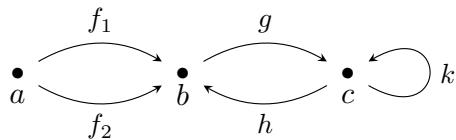
\includegraphics[keepaspectratio]{images/part001_552ae758.jpg}}

表示一个箭图，其顶点为 a、b、c，其箭为 \(f_{1}, f_{2}, g, h, k\) ，且源映射与靶映射由下式给出

\[
\begin{array}{c c c c} o (f _ {1}) = o (f _ {2}) = a & \quad o (g) = b & \quad o (h) = c & \quad o (k) = c \\ t (f _ {1}) = t (f _ {2}) = b & \quad t (g) = c & \quad t (h) = b & \quad t (k) = c. \end{array}
\]

\subsection{子箭图}

设 C 与 C′ 为箭图。若 \(\operatorname{Som}(\mathrm{C}') \subset \operatorname{Som}(\mathrm{C})\) ，\(\operatorname{Fl}(\mathrm{C}') \subset \operatorname{Fl}(\mathrm{C})\) ，且映射 \(o_{C'}\) 与 \(t_{C'}\) 分别与映射 \(o_{C}\) 与 \(t_{C}\) 在 \(\operatorname{Fl}(\mathrm{C}')\) 上相合，则称 C′ 是 C 的子箭图。此外，若 C 中源与靶都属于 \(\operatorname{Som}(\mathrm{C}')\) 的每个箭都是 C′ 的箭，则称 C′ 是 C 的全子箭图。

设 C 为箭图，\((\mathrm{C}_{i})_{i\in\mathrm{I}}\) 为 C 的子箭图族。称族 \((\mathrm{C}_{i})_{i\in\mathrm{I}}\) 的交，并记作 \(\bigcap_{i\in I}C_{i}\) ，这样的 C 的子箭图：其顶点集为 \(\bigcap_{i\in I}\mathrm{Som}(\mathrm{C}_{i})\) ，其箭集为 \(\bigcap_{i\in I}\mathrm{Fl}(\mathrm{C}_{i})\) 。

\subsection{箭图的态射}

设 C 与 C' 为箭图。从 C 到 C' 的箭图态射是一个偶 \((u,v)\) ，其中 \(u\colon\operatorname{Som}(\mathrm{C})\to\operatorname{Som}(\mathrm{C}')\) 与 \(v\colon\operatorname{Fl}(\mathrm{C})\to\operatorname{Fl}(\mathrm{C}')\) 是满足 \(o_{C'}\circ v=u\circ o_{C}\) 与 \(t_{C'}\circ v=u\circ t_{C}\) 的映射。

设 \(\varphi = (u, v)\) 为从 C 到 C' 的箭图态射。映射 \(u\) 与 \(v\) 分别记作 \(\operatorname{Som}(\varphi)\) 与 \(\operatorname{Fl}(\varphi)\) 。若 \(a\) 是 C 的顶点，则滥用记号，把 \(\varphi(a)\) 记为顶点 \(a\) 在 \(\varphi\) 下的象，我们将说 \(\varphi(a)\)

是 \(a\) 在 \(\varphi\) 下的象。类似地，若 \(f\) 是 C 的箭，则滥用记号，把 \(\varphi(f)\) 记为 C' 的箭 \(v(f)\) ，我们将说它是 \(f\) 在 \(\varphi\) 下的象。

设 C、\(C'\) 、\(C''\) 为三个箭图，\(\varphi = (u, v)\) 为从 C 到 \(C'\) 的态射，\(\varphi' = (u', v')\) 为从 \(C'\) 到 \(C''\) 的态射。则 \((u' \circ u, v' \circ v)\) 是从 C 到 \(C''\) 的态射，记作 \(\varphi' \circ \varphi\) ，称为 \(\varphi'\) 与 \(\varphi\) 的复合。

我们把 \(\mathrm{Id}_{\mathrm{C}}\) 记为从 C 到自身的态射 \((\mathrm{Id}_{\mathrm{Som}(\mathrm{C})}, \mathrm{Id}_{\mathrm{Fl}(\mathrm{C})})\) 。

设 \(\varphi\) 为从 C 到 C' 的箭图态射。为使 \(\varphi\) 是同构，必须且只需映射 \(\operatorname{Som}(\varphi)\) 与 \(\operatorname{Fl}(\varphi)\) 都是双射（参见 E, IV, 第 6 页）。

这样，若把集合 S 与 F 上的箭图结构称为两个映射 \(o, t: \mathrm{F} \to \mathrm{S}\) 的数据，就可以把箭图态射取作这个结构的态射（E, IV, 第 11 页）。

设 \(\varphi\) 为从 C 到 C' 的箭图态射。存在 C' 的唯一子箭图，其顶点集与箭集分别是 \(\mathrm{Som}(\varphi)\) 与 \(\mathrm{Fl}(\varphi)\) 的象。把它记作 \(\varphi(\mathrm{C})\) ，称为 C 在 \(\varphi\) 下的象。称 \(\varphi\) 是单射的，若映射 \(\mathrm{Som}(\varphi)\) 与 \(\mathrm{Fl}(\varphi)\) 都是单射；这时 \(\varphi\) 诱导一个从 C 到其象上的同构。

设 \(\varphi\) 与 \(\psi\) 为从 C 到 C' 的箭图态射。存在 C 的唯一子箭图，其顶点与箭分别是 C 中在 \(\varphi\) 与 \(\psi\) 下有相同象的顶点与箭。我们称之为 \(\varphi\) 与 \(\psi\) 的均衡子。

\subsection{箭图的积}

设 \((\mathrm{C}_{i})_{i\in\mathrm{I}}\) 为箭图族。令 \(S = \prod_{i\in\mathrm{I}} \mathrm{Som}(\mathrm{C}_{i})\) ，\(F = \prod_{i\in\mathrm{I}} \mathrm{Fl}(\mathrm{C}_{i})\) ，并设 o 与 t 分别为映射 \(\prod_{i\in\mathrm{I}} o_{C_{i}}\) 与 \(\prod_{i\in\mathrm{I}} t_{C_{i}}\) 。四元组 \(C = (S, F, o, t)\) 是一个箭图，称为族 \((\mathrm{C}_{i})_{i\in\mathrm{I}}\) 的积箭图。

存在唯一的箭图态射 \(pr_{i}: C \to C_{i}\) ，使得映射 \(\operatorname{Som}(\operatorname{pr}_{i})\) 与 \(\operatorname{Fl}(\operatorname{pr}_{i})\) 分别是从 \(\operatorname{Som}(C)\) 到 \(\operatorname{Som}(C_{i})\) 上与从 \(\operatorname{Fl}(C)\) 到 \(\operatorname{Fl}(C_{i})\) 上的指标 i 投影。

我们有下列泛性质：设 C' 为箭图；对任何族 \((\varphi_{i})_{i\in\mathrm{I}}\) ，其中对每个 \(i\in I\) ，\(\varphi_{i}\colon C'\to C_{i}\) 是箭图态射，存在唯一的箭图态射 \(\varphi\colon\mathrm{C}^{\prime}\to\mathrm{C}\) ，使得 \(\varphi_{i}=\mathrm{pr}_{i}\circ\varphi\) （对所有 \(i\in\mathrm{I}\) ）。

\subsection{箭图中的道路与圈}

定义 2. —— 设 C 为箭图。C 中的道路是一个序列 \(c = (a_{0}, f_{1}, a_{1}, \ldots, a_{n-1}, f_{n}, a_{n})\) ，其中 \(n\) 是整数 \(\geqslant 0\) ，\(a_{0}, \ldots, a_{n}\) 是 C 的顶点，且对 \(1 \leqslant i \leqslant n\) ，\(f_{i}\) 是 C 中连接 \(a_{i-1}\) 与 \(a_{i}\) 的箭。我们说道路 c 的长度为 \(n\) 。

设 \(c = (a_{0}, f_{1}, a_{1}, \ldots, a_{n-1}, f_{n}, a_{n})\) 为 C 中长度为 n 的道路。顶点 \(a_{0}\) 称为 c 的起点或源；顶点 \(a_{n}\) 称为 c 的终点或靶；也说 c 连接顶点 \(a_{0}\) 与顶点 \(a_{n}\) 。顶点 \(a_{i}\) （\(0 \leqslant i \leqslant n\)）称为指标 i 的顶点；箭 \(f_{i}\) （\(1 \leqslant i \leqslant n\)）称为第 i 个箭，或指标 i 的箭。长度 \(\geqslant 1\) 的道路由其箭的序列确定。

起点与终点相同的道路称为圈。长度为 0 的道路是圈，称为常值圈。

我们说道路

\[
c = (a _ {0}, f _ {1}, a _ {1}, \ldots , a _ {n - 1}, f _ {n}, a _ {n}) \text{且} c ^ {\prime} = (a _ {0} ^ {\prime}, f _ {1} ^ {\prime}, a _ {1} ^ {\prime}, \ldots , a _ {m - 1} ^ {\prime}, f _ {m} ^ {\prime}, a _ {m} ^ {\prime})
\]

在 C 中是可并列的，如果 c 的终点 \(a_{n}\) 是起点 \(a_{0}^{\prime}\) （\(c^{\prime}\) 的）。这时，序列 \((a_{0}, f_{1}, a_{1}, \ldots, a_{n-1}, f_{n}, a_{n}, f_{1}^{\prime}, a_{1}^{\prime}, \ldots, f_{m}^{\prime}, a_{m}^{\prime})\) 是 C 中的道路，记作 \(c * c^{\prime}\) ，称为 c 与 \(c^{\prime}\) 的并列道路。它连接 c 的起点与 \(c^{\prime}\) 的终点；其长度是道路 c 与 \(c^{\prime}\) 的长度之和。

\subsection{箭图的连通分支}

设 \(C = (S, F, o, t)\) 为箭图。考虑 S 上的等价关系 \(R_{C}\) ，即使得对 C 的每个箭 f 关系 \(\mathrm{R}_{\mathrm{C}}\{o(f), t(f)\}\) 成立的最细者。C 的两个顶点 a、b 对这个关系等价，当且仅当存在整数 \(n \geqslant 0\) 、C 的顶点 \(a_{0}, \ldots, a_{n}\) 与 C 的箭 \(f_{1}, \ldots, f_{n}\) ，使得 \(a_{0} = a\) ，\(a_{n} = b\) ，且对 \(1 \leqslant i \leqslant n\) ，箭 \(f_{i}\) 或者连接 \(a_{i-1}\) 与 \(a_{i}\) ，或者连接 \(a_{i}\) 与 \(a_{i-1}\) 。

这个等价关系的等价类称为 C 的连通分支。以 \(\pi_0(\mathrm{C})\) 表示 C 的连通分支所成的集。最后，若 C 至多有一个连通分支，则称 C 是连通的。

设 \(\varphi\colon\mathrm{C}\to\mathrm{C}^{\prime}\) 为箭图态射。映射 \(\operatorname{Som}(\varphi)\) 通过过渡到商，定义了一个从 \(\pi_{0}(\mathrm{C})\) 到 \(\pi_{0}(\mathrm{C}^{\prime})\) 的映射，我们把它记作 \(\pi_{0}(\varphi)\) 。

\section{图}

\subsection{图的定义}

定义 1. —— 图 \(^{(1)}\) 是一个箭图 (S, F, o, t)，带有一个 F 的对合，记作 \(f \mapsto \overline{f}\) ，它没有不动点，且满足 \(t(\overline{f}) = o(f)\) （对所有 \(f \in F\) ）。

称箭图 (S, F, o, t) 为这个图的底箭图。对这个箭图的每个箭 f，按定义有 \(\overline{\overline{f}} = f\) 、\(\overline{f} \neq f\) 与 \(t(\overline{f}) = o(f)\) 。把最后这个关系应用于箭 \(\overline{f}\) ，就得到等式 \(o(\overline{f}) = t(f)\) 。箭 \(\overline{f}\) 称为 f 的相反箭。

图的一对相反箭称为图的一条边。属于这个偶的两个箭中的每一个都称为这条边的一个定向。因此，图的箭也称为图的定向边。

若 G 与 G' 是图，从 G 到 G' 的图态射是箭图态射 \(\varphi\colon\mathrm{G}\to\mathrm{G}'\) ，它满足 \(\overline{\varphi(f)}=\varphi(\overline{f})\) （对 G 的每个箭 \(f\) ）。

设 G 与 G' 为图；若 G' 是子箭图且 Fl(G') 的对合是 Fl(G) 的对合的限制，则称 G' 是 G 的子图。

\subsection{图的定向}

设 G 为图。G 的一个定向是 G 的箭集的一个子集 A，满足 \(A \cap \overline{A} = \varnothing\) 且 \(A \cup \overline{A} = \mathrm{Fl}(G)\) 。

带有一个定向的图称为定向图。

设 G 为定向图，A 为其定向；G 的定向子图是子图 \(G'\) （G 的），带有定向 \(A' = \mathrm{Fl}(G') \cap A\) 。

设 (G, A) 与 (G', A') 为定向图。从 (G, A) 到 (G', A') 的定向图态射是图态射 \(\varphi\colon G \to G'\) ，满足 \(\operatorname{Fl}(\varphi)(A) \subset A'\) 。

\subsection{定向图与箭图}

设 G 为图，\((S,F,o,t)\) 为其底箭图，A 为 G 的一个定向。则 \((S,A,o\mid A,t\mid A)\) 是一个箭图，称为与定向图 \((G,A)\) 伴随的箭图。

反之，设 \(C = (S, F, o, t)\) 为箭图。令 \(\widetilde{F} = F \times \{-1, 1\}\) ，并设 \(\widetilde{o}, \widetilde{t}\) 为由下式定义的从 \(\widetilde{F}\) 到 S 的映射

\[
\begin{array}{l l} \widetilde {o} (f, 1) = o (f) & \qquad \qquad \widetilde {o} (f, - 1) = t (f) \\ \widetilde {t} (f, 1) = t (f) & \qquad \qquad \widetilde {t} (f, - 1) = o (f), \end{array}
\]

对每个 \(f \in \mathrm{F}\) 。于是，\(\widetilde{\mathrm{C}} = (\mathrm{S}, \widetilde{\mathrm{F}}, \widetilde{o}, \widetilde{t})\) 赋有对合 \((f, \varepsilon) \mapsto (f, -\varepsilon)\) （\(\widetilde{\mathrm{F}}\) 的），是一个图，称为与箭图 C 伴随的图。集 \(\mathrm{A} = \mathrm{F} \times \{1\}\) 是这个图的一个定向。称 \((\widetilde{\mathrm{C}}, \mathrm{A})\) 为与箭图 C 伴随的定向图。

若 \(f\) 是 C 的箭，也说 \((f,1)\) 是 \(\widetilde{C}\) 的与 \(f\) 伴随的定向边，且偶 \(\{(f,1),(f,-1)\}\) 是 \(\widetilde{C}\) 的与 \(f\) 伴随的边。

若 C' 是 C 的子箭图，则定向图 \(\widetilde{C}'\) 是 \(\widetilde{C}\) 的定向子图。

存在唯一的箭图态射 \(\varphi\) （从 C 到 \(\widetilde{\mathrm{C}}\) 的底箭图），使得 \(\varphi(f) = (f,1)\) （对 C 的每个箭 \(f\) ）；它是从 C 到与定向图 ( \(\widetilde{\mathrm{C}}\) , A) 伴随的箭图上的同构。

\subsection{树}

当谈到图的道路或连通分支时，指的是底箭图的道路或连通分支。图的两个顶点属于同一连通分支，当且仅当存在连接它们的道路。

设 G 为图。若 \(c = (a_{0}, f_{1}, a_{1}, \ldots, f_{n}, a_{n})\) 是 G 中的道路，则序列 \(\overline{c} = (a_{n}, \overline{f_{n}}, \ldots, a_{1}, \overline{f_{1}}, a_{0})\) 是 G 中的道路，称为 c 的相反道路。设 c 与 \(c'\) 是 G 中可并列的道路；则 \(\overline{c'}\) 与 \(\overline{c}\) 可并列，且有 \(\overline{c * c'} = \overline{c'} * \overline{c}\) 。

若 c 中没有一对相邻的箭是相反的，则称 G 中的道路 c 是无回溯的。设 \(c = (a_{0}, f_{1}, \ldots, f_{n}, a_{n})\) 为 G 中连接 \(a_{0}\) 与 \(a_{n}\) 的道路。若对满足 \(1 \leqslant i < n\) 的整数 i，箭 \(f_{i}\) 与 \(f_{i+1}\) 相反，则 \((a_{0}, f_{1}, \ldots, a_{i-1}, f_{i+2}, \ldots, f_{n}, a_{n})\) 是 G 中连接 \(a_{0}\) 与 \(a_{n}\) 的道路，其长度严格小于道路 c 的长度。由归纳法，因此存在 G 中连接 \(a_{0}\) 与 \(a_{n}\) 的无回溯道路。

定义 2. —— 森林是这样的图：其中每条无回溯的圈都是常值圈。树是连通的森林。

命题 1. —— 设 G 为图。G 的每个森林都含于 G 的一个极大森林中；特别地，存在 G 的极大森林。

为使 G 的森林是极大的，必须且只需其顶点集等于 G 的顶点集，且其连通分支就是 G 的连通分支。

设 \(A_{0}\) 为 G 的森林。G 的森林所成的集，赋有序关系“A 是 B 的子图”后，是归纳的。因此，存在 G 的极大森林，\(A_{0}\) 是它的子图（E, III, 第 21 页, 推论 1）。

以 \(\operatorname{Som}(G)\) 为顶点集、箭集为空的 G 的子图是 G 的森林。因此存在 G 的极大森林。

设 A 为 G 的极大森林。我们证明 A 与 G 有相同的顶点集。以 \(\operatorname{Som}(G)\) 为顶点集、以 \(\operatorname{Fl}(A)\) 为箭集的 G 的子图是一个森林，且 A 是它的子图。于是有 \(\operatorname{Som}(A) = \operatorname{Som}(G)\) 。

现在证明 A 与 G 有相同的连通分支。由于 A 的每个箭都是 G 的箭，A 的每个连通分支含于 G 的一个连通分支。既然 A 与 G 有相同的顶点集，只需证明 G 中处于同一连通分支的两个顶点也处于 A 的同一连通分支。若不然，关系 \(R_{A}\) （“处于 A 的同一连通分支”）严格细于关系 \(R_{G}\) ，且存在 G 的两个顶点，它们不处于 A 的同一连通分支，但却被 G 的一个箭 f 连接。设 B 为 G 的定向子图，其顶点集为 \(\operatorname{Som}(G)\) ，箭集为 \(\mathrm{Fl(A)} \cup \{f, \overline{f}\}\) 。我们来证明 B 是 G 的森林。设 \(c = (a_{0}, f_{1}, \ldots, f_{n}, a_{n})\) 为 B 中长度最小的非常值无回溯圈。由于 A 是森林，圈 c 不是 A 中的圈。设 i（相应地，j）为 \(\{0, \ldots, n\}\) 中使 \(a_{0}\) 与 \(a_{i}\) （相应地，\(a_{j}\) 与 \(a_{n}\) ）不处于 A 的同一连通分支的最小（相应地，最大）整数。这意味着箭 \(f_{i}\) 与 \(f_{j+1}\) 是 B 中与边 \(\{f, \overline{f}\}\) 伴随的定向箭，且它们相反。由于圈 c 无往返，\(f_{i+1} \neq \overline{f_{i}}\) ，因此 \(i \neq j\) ，而道路 \((a_{i}, f_{i+1}, a_{i+1}, \ldots, f_{j}, a_{j})\) 是 B 中长度 < n 的非常值无回溯圈，与 c 长度最小的假设矛盾。由此推出 B 是森林。这与 A 是 G 的极大森林的假设矛盾。

现设 A 为 G 的森林，满足 \(\mathrm{Som}(\mathrm{A}) = \mathrm{Som}(\mathrm{G})\) 与 \(\pi_{0}(\mathrm{A}) = \pi_{0}(\mathrm{G})\) 。我们来证明它是 G 的极大森林。只需证明：若 \(f \notin \mathrm{Fl}(\mathrm{A})\) ，则 G 的以 \(\mathrm{Som}(\mathrm{G})\) 为顶点集、以 \(\mathrm{Fl}(\mathrm{A}) \cup \{f, \overline{f}\}\) 为箭集的子图 B 不是森林。按假设，点 \(o(f)\) 与 \(t(f)\) 处于 A 的同一连通分支；因此存在 A 中连接 \(o(f)\) 与 \(t(f)\) 的无回溯道路 c。于是道路 \(c * \overline{f}\) 是 B 中无回溯且非常值的圈，这表明 B 不是森林。

推论. —— 连通图的极大森林是它的极大树。

注 1. —— 在 LIE, IV, 第 33 页附录中，组合图的概念定义为偶 (A, S)，其中 S 是一个集合，

而 A 是 \(\mathfrak{P}(S)\) 的由二元集组成的子集；S 的元素称为顶点，A 的元素称为边，且两个顶点 \(x\) 与 \(y \in S\) 称为相连的，如果 \(\{x, y\}\) 是一条边。

对这样的组合图 \(\Gamma = (\mathrm{A},\mathrm{S})\) ，伴随一个图 G，其顶点集为 S，箭集 \(\widetilde{\mathrm{A}}\) 是 \(\mathrm{S}^2\) 中由相连顶点的偶所组成的子集，其源映射与靶映射分别与 \(\mathrm{S}^2\) 到 S 的第一、第二投影相合，而对合 \(f\mapsto \overline{f}\) 由 \(\widetilde{\mathrm{A}}\) 上的映射 \((x,y)\mapsto (y,x)\) （\(\mathrm{S}^2\) 到自身的）的限制给出。把 G 的边 \(\{f,\overline{f}\}\) 映为集合 \(\{o(f),t(f)\}\) 的映射是从 G 的边集到组合图 \(\Gamma\) 的边集上的双射。

反之，每个使得每个箭的源与靶不同、且箭由其源与靶确定的图，都具有这种形式。

读者可以验证，组合图的连通性、树或森林的概念，与与之伴随的图的相应概念一致。

\section{群胚}

\subsection{范畴}

定义 1. —— 设 C 为箭图。以 J 表示 C 中箭的偶 \((f,g)\) （满足 \(t(f)=o(g)\) ）所成的集。C 上的一个合成律是这样的映射 \(m:J\to\mathrm{Fl}(\mathrm{C})\) ：对每个偶 \((f,g)\in\mathrm{J}\) ，箭 \(m(f,g)\) 的起点是 f 的起点，其靶是 g 的靶。

设 C 为带有一个合成律 \(m\) 的箭图。两个箭 \(f\) 与 \(g\) （满足 \(t(f) = o(g)\) ）称为可复合的；箭 \(m(f, g)\) 称为它们的复合，或它们的乘积，常记作 \(f \cdot g\) ，甚至记作 \(fg\) 。

对 C 的每个顶点 \(a\) ，集合 \(\mathrm{C}_{a,a} = \mathrm{Fl}_{a,a}(\mathrm{C})\) 赋有由 \(m\) 过渡到子集而得的映射后，是一个群原（A, I, 第 1 页, 定义 1）。

C 的箭的族 \((f_{i})_{i\in\mathrm{I}}\) ，以有限非空全序集 I 为指标集，若对 I 的每对相邻元素 \((i,j)\) ，箭 \(f_{i}\) 与 \(f_{j}\) 可复合，则称该族是可复合的。这样的族的乘积 \(\prod_{i\in\mathrm{I}}f_{i}\) 由对 I 的基数用归纳法定义如下（参见 A, I, 第 3 页）：

\begin{enumerate}
\def\labelenumi{(\roman{enumi})}
\item
  若 I 只有一个元素 \(\omega\) ，则 \(\prod_{i\in I}f_i = f_\omega\) ；
\item
  若 I 至少有两个元素且 \(\omega\) 是 I 的最小元素，则令 \(\prod_{i\in I}f_i = f_\omega \cdot \prod_{i\in I - \{\omega \}}f_i\) 。
\end{enumerate}

合成律 \(m\) 称为结合的，若 \(f \cdot (g \cdot h) = (f \cdot g) \cdot h\) （对 C 的箭的每个可复合三元组 \((f, g, h)\) ）。当律 \(m\) 结合时，序列 \((f_1, \ldots, f_n)\) （\(n\) 个可复合箭的，其中 \(n\) 为整数 \(\geqslant 1\) ）的乘积记作 \(f_1 f_2 \ldots f_n\) 。

设 \(a\) 为 C 的顶点。称箭 \(e \in \mathrm{C}_{a,a}\) 是 \(m\) 在 \(a\) 处的单位元，若 \(ef = f\) （对每个箭 \(f\) ，以 \(a\) 为源的），且 \(ge = g\) （对每个箭 \(g\) ，以 \(a\) 为终点的）。\(m\) 在 \(a\) 处至多有一个单位元：若 \(e\) 与 \(e'\) 是两个单位元，则有 \(e' = ee' = e\) 。当这样的单位元存在时，常记作 \(e_a\) ；它这时是群原 \(\mathrm{C}_{a,a}\) 的单位元（A, I, 第 12 页）。

定义 2. —— 范畴是带有一个结合合成律的箭图，且在每个顶点处存在单位元。

例. —— 1) 设 C 为箭图。以 Ch(C) 表示 C 中道路所成的集，以 o: Ch(C) → Som(C)、t: Ch(C) → Som(C) 表示把道路映为其起点与终点的映射。四元组 \(\Omega_{\mathrm{C}} = (\mathrm{Som}(\mathrm{C}), \mathrm{Ch}(\mathrm{C}), o, t)\) 是一个箭图。给它赋予由道路的衔接定义的合成律。这个合成律是结合的；对 C 的每个顶点 a，以 a 为起点的常值圈 \(e_a = (a)\) 是 a 处的单位元。这样，\(\Omega_{\mathrm{C}}\) 是一个范畴。称之为箭图 C 的道路范畴。

\begin{enumerate}
\def\labelenumi{\arabic{enumi})}
\setcounter{enumi}{1}
\tightlist
\item
  设 \(\Sigma\) 为比集合论更强的理论 \(\mathcal{T}\) 中的一种结构，\(\sigma\{x,y,s,u\}\) 为 \(\mathcal{T}\) 中满足 E, IV, 第 11 页的条件 (MO \(_{\text{I}}\) )、(MO \(_{\text{II}}\) ) 与 (MO \(_{\text{III}}\) ) 的项。设 S 为集合；假设 S 的每个元素都是偶 \((x,s)\)，其中 \(x\) 是集合，\(s\) 是种 \(\Sigma\) 的结构（在 \(x\) 上的）。设 F 为这样的映射 \(f\) 所成的集：存在 S 中的 \((x,s)\) 与 \((y,t)\) ，使 \(f\) 是一个 \(\sigma\) -态射，从 \(x\) （赋有结构 \(s\) 的）到 \(y\) （赋有结构 \(t\) 的）；这时令 \(o(f) = (x,s)\) 与 \(t(f) = (y,t)\) 。赋有由 \(m(f,g)=g\circ f\) 给出的合成律后，箭图 (S,F,o,t) 是一个范畴。在这种语境下，S 的元素更常称为对象。
\end{enumerate}

设 C 为范畴。

对 C 的每个顶点 \(a\) ，集合 \(\mathrm{C}_{a,a}\) 赋有合成律 \((f,g)\mapsto fg\) 后，是以 \(e_a\) 为单位元的幺半群。

称 C 的箭 \(f\) 是可逆的，若存在 C 的箭 \(g\) ，使得 \(o(g) = t(f)\) 、\(t(g) = o(f)\) ，且 \(fg\) 与 \(gf\) 分别是 \(o(f)\) 与 \(t(f)\) 处的单位元。这样的箭 \(g\) 是唯一的（若 \(fg = e_{o(f)}\) 且 \(g'f = e_{t(f)}\) ，则有 \(g = e_{t(f)}g = (g'f)g = g'(fg) = g'e_{o(f)} = g'\) ），称为 \(f\) 的逆；可逆箭 \(f\) 的逆记作 \(f^{-1}\) 。

\subsection{函子}

定义 3. —— 设 C 与 C' 为范畴。从 C 到 C' 的函子是箭图态射 \(\varphi\colon\mathrm{C}\to\mathrm{C}'\) ，满足 \(\varphi(fg)=\varphi(f)\varphi(g)\) （对 C 的每对可复合箭 \((f,g)\) ）。

设 C 与 C' 为范畴，\(\varphi\colon\mathrm{C}\to\mathrm{C}'\) 为函子。设 \(f\) 为 C 的箭，\(a\) 为其起点，\(b\) 为其靶；则 \(\varphi(f)\) 是 C' 的箭，起点为 \(\varphi(a)\) ，靶为 \(\varphi(b)\) 。

设 C、C'、C'' 为范畴，\(\varphi\colon\mathrm{C}\to\mathrm{C}'\) 与 \(\varphi'\colon\mathrm{C}'\to\mathrm{C}''\) 为函子。则 \(\varphi'\circ\varphi\) 是函子。

设 C 为范畴。则箭图态射 \(Id_{C}\) 是函子。

设 \(\varphi\colon\mathrm{C}\to\mathrm{C}^{\prime}\) 为函子。为使 \(\varphi\) 是同构，必须且只需映射 \(\operatorname{Som}(\varphi)\) 与 \(\operatorname{Fl}(\varphi)\) 都是双射。

这样，若把集合 S 与 F 上的范畴结构称为这些集合上的箭图结构与一个在每个顶点处存在单位元的结合合成律的数据，就可以把函子取作这个范畴结构的态射（E, IV, 第 11 页）。

\subsection{群胚}

定义 4. —— 群胚是每个箭都可逆的范畴。

设 G 为群胚，a 为 G 的顶点。幺半群 \(G_{a,a}\) 是一个群，记作 \(G_{a}\) ，称为 G 在 a 处的迷向群。

设 \(a\) 与 \(b\) 为 G 的顶点，\(f \in \mathrm{G}_{a,b}\) 为连接 \(a\) 与 \(b\) 的箭。映射 \(g \mapsto fgf^{-1}\) 是从 \(\mathrm{G}_b\) 到 \(\mathrm{G}_a\) 的群同构，记作 \(\operatorname{Int}(f)\) 。若 \(f\) 与 \(f'\) 是 G 的可复合箭，则有 \(\operatorname{Int}(ff') = \operatorname{Int}(f) \circ \operatorname{Int}(f')\) 。同构 \(\operatorname{Int}(f)\) 的逆是同构 \(\operatorname{Int}(f^{-1})\) 。

群胚态射 \(\varphi\colon G\to G'\) 是范畴态射。此外，\(\varphi\) 是群胚同构当且仅当它是范畴同构。

设 \(\varphi\colon\mathrm{G}\to\mathrm{G}^{\prime}\) 为群胚态射。对 G 的每个顶点 \(a\) ，映射 \(f\mapsto\varphi(f)\) （从 \(\mathrm{G}_{a}\) 到 \((\mathrm{G}^{\prime})_{\varphi(a)}\) 的）是群同态，记作 \(\varphi_{a}\) 。特别地，有 \(\varphi(e_{a})=e_{\varphi(a)}\) 。

对 G 的每个箭 \(f\) ，\(\varphi(f^{-1})\) 是 \(\varphi(f)\) 的逆。若 \(f\) 是 G 中连接顶点 \(a\) 与顶点 \(b\) 的箭，则对每个元素 \(g \in \mathrm{G}_b\) ，有关系 \(\operatorname{Int}(\varphi(f))(\varphi(g)) = \varphi(\operatorname{Int}(f)(g))\) 。

\subsection{群胚的轨道}

设 G 为群胚。G 的底箭图的连通分支称为 G 的轨道。G 的轨道所成的集记作 \(\mathrm{Orb}(\mathrm{G})\) ；若 \(\varphi: G \to G'\) 是群胚态射，则映射 \(\pi_{0}(\varphi)\) （由 \(\varphi\) 过渡到伴随图的连通分支而得的）通常记作 \(\mathrm{Orb}(\varphi)\) ，称为由 \(\varphi\) 过渡到轨道而得的映射。

恰有一个轨道的群胚称为传递的。若 G 是传递群胚，则诸群 \(G_{a}\) （对 \(a \in \text{Som}(G)\) ）彼此同构。若群胚 G 是传递的，且诸迷向群 \(G_{a}\) 都缩为各自的单位元，则称群胚 G 是单传递的。

命题 1. —— 设 G 为群胚。关系“存在 G 的箭连接 a 与 b”是 G 的顶点集上的等价关系，其等价类即 G 的轨道。

设 \(a\) 、\(b\) 、\(c\) 为 G 的顶点。我们有 \(e_a \in \mathrm{G}_{a,a}\) ；若 \(f \in \mathrm{G}_{a,b}\) ，则 \(f^{-1} \in \mathrm{G}_{b,a}\) ；若 \(f \in \mathrm{G}_{a,b}\) 且 \(g \in \mathrm{G}_{b,c}\) ，则有 \(fg \in \mathrm{G}_{a,c}\) 。这表明所指的关系是自反的、对称的且传递的；因此是等价关系。第二个断言由箭图连通分支的定义得出。

\subsection{群胚的例子}

\begin{enumerate}
\def\labelenumi{\arabic{enumi})}
\item
  设 G 为群。以 \(\mathcal{G}\) 表示这样的箭图：其顶点集缩为单个元素，其箭集为 G。\(\mathcal{G}\) 赋有由 G 的合成律诱导的合成律后，是一个群胚，称为与群 G 伴随的群胚。
\item
  设 X 为集合。设 G 为箭图 \((\mathrm{X}, \mathrm{X} \times \mathrm{X}, \mathrm{pr}_{1}, \mathrm{pr}_{2})\) ；在 G 上定义合成律：令 \((x, x') \cdot (x', x'') = (x, x'')\) （若 \(x, x', x''\) 是 X 的元素）。这个律是结合的；对每个 \(x \in X\) ，\((x, x)\) 是 x 处的中性元；箭 \((x, x')\) 的逆是箭 \((x', x)\) 。这样定义的群胚称为集合 X 的偶对群胚。若 X 非空，它是单传递的。
\item
  设 X 与 S 为集合，\(p \colon \mathrm{X} \to \mathrm{S}\) 为映射。对 \(a \in \mathrm{S}\) ，记 \(\mathrm{X}_a = p^{-1}(a)\) 。对 S 中的 \(a\) 与 \(b\) ，设 \(\mathrm{G}_{a,b}\) 为集 \(\mathcal{B}(\mathrm{X}_a; \mathrm{X}_b)\) （从 \(\mathrm{X}_a\) 到 \(\mathrm{X}_b\) 的双射所成的），并设 G 为诸集 \(\mathrm{G}_{a,b}\) 的不交并。设 \(o\) 与 \(t\) 为从 G 到 S 的映射，使得 \(o(f) = a\) 与 \(t(f) = b\) （对每个元素 \(f \in \mathrm{G}_{a,b}\) ）。四元组 \((\mathrm{S}, \mathrm{G}, o, t)\) 是一个箭图。给它赋予由 \(m(f, g) = g \circ f\) （若 \(f \in \mathcal{B}(\mathrm{X}_a; \mathrm{X}_b)\) 且 \(g \in \mathcal{B}(\mathrm{X}_b; \mathrm{X}_c)\) ，其中 \(a, b, c\) 是 S 的元素）定义的合成律。这是一个群胚；记作 \(\mathcal{B}(\mathrm{X}, p)\) ，称为 X 相对于 \(p\) 的置换群胚。
\item
  设 \((\mathrm{G}_{i})_{i\in\mathrm{I}}\) 为群胚族。以 G 表示诸底箭图族的积箭图；对每个 \(i\in I\) ，设 \(pr_{i}\colon G\to G_{i}\) 为典范箭图态射。G 上存在唯一的合成律，使 G 成为群胚，且对每个 \(i \in I\) ，\(\mathrm{pr}_i\) 是群胚态射。设 \(f = (f_i)_{i \in I}\) 与 \(g = (g_i)_{i \in I}\) 为 G 的箭；它们可复合，当且仅当箭 \(f_i\) 与 \(g_i\) 可复合（对 \(i \in I\) ）。这时有 \(fg = (f_i g_i)_{i \in I}\) 。
\end{enumerate}

箭图 G 赋有这个合成律后，称为族 \((\mathrm{G}_{i})_{i\in\mathrm{I}}\) 的积群胚。它满足下列泛性质：对每个群胚 \(G'\) 与每个族 \((\varphi_{i})_{i\in\mathrm{I}}\) （其中 \(\varphi_{i}\) 是从 \(G'\) 到 \(G_{i}\) 的群胚态射），存在唯一的群胚态射 \(\varphi: G'\to G\) ，使得 \(\varphi_{i}=\operatorname{pr}_{i}\circ\varphi\) （对所有 \(i\in I\) ）。

\begin{enumerate}
\def\labelenumi{\arabic{enumi})}
\setcounter{enumi}{4}
\tightlist
\item
  设 \(((\mathrm{G}_{i})_{i\in\mathrm{I}},(\varphi_{i,j})_{i\prec j})\) 为群胚的归纳系，以右过滤预序集 \((\mathrm{I},\prec)\) 为指标集，其中 \(\varphi_{i,j}\) 是群胚态射。设 G 为这样的箭图：其顶点集为 \(\varinjlim_{i}\operatorname{Som}(\mathbf{G}_{i})\) ，箭集为 \(\varinjlim_{i}\operatorname{Fl}(\mathbf{G}_{i})\) ，源映射与靶映射分别为映射 \(\varinjlim_{i}o_{G_{i}}\) 与 \(\varinjlim_{i}t_{G_{i}}\) 。诸 \(G_{i}\) 的合成律在 G 上诱导一个合成律，使 G 成为群胚（参见 A, I, 第 114 页）。典范映射 \(\operatorname{Som}(\mathbf{G}_{i})\to\operatorname{Som}(\mathbf{G})\) 与 \(\operatorname{Fl}(\mathbf{G}_{i})\to\operatorname{Fl}(\mathbf{G})\) 定义了一个群胚态射 \(\varphi_{i}\) （从 \(G_{i}\) 到 G 的）。若 i、j 是 I 中满足 \(i\prec j\) 的元素，则有 \(\varphi_{j}\circ\varphi_{i,j}=\varphi_{i}\) 。群胚 G 称为群胚族 \(G_{i}\) 的归纳极限，记作 \(\varinjlim_{i}G_{i}\) 。它满足下列泛性质：对每个群胚 H 与每个族 \((\psi_{i})_{i\in\mathrm{I}}\) （其中对 \(i\in I\) ，\(\psi_{i}:G_{i}\to H\) 是群胚态射，并且 \(\psi_{j}\circ\varphi_{i,j}=\psi_{i}\) 对 I 的元素的每对 \((i,j)\) （满足 \(i\prec j\) ）成立），存在唯一的群胚态射 \(\psi:G\to H\) 使得 \(\psi_{i}=\psi\circ\varphi_{i}\) 。
\end{enumerate}

关于当不假设集 I 右过滤时满足这个泛性质的群胚的存在性，参见 II, 第 228 页, 习题 3。

\subsection{子群胚}

定义 5. —— 设 C 为范畴。C 的子范畴是 C 的满足下列条件的子箭图 D：

\begin{enumerate}
\def\labelenumi{(\roman{enumi})}
\item
  对 D 的每个顶点 a，\(e_a\) 是 D 的箭；
\item
  对 C 中属于 D 的每对可合成箭 \((f,g)\) ，积 fg 是 D 的箭；
\end{enumerate}

设 C 为范畴，D 为 C 的子范畴；赋有把 C 的合成法则限制到子集上而诱导的合成法则，D 是一个范畴。

C 的每个全子箭图都是 C 的子范畴。C 的一族子范畴的交是 C 的子范畴。

定义 6. —— 设 G 为群胚。G 的子群胚是 G 的这样一个子范畴 H：G 中属于 H 的每个箭的逆都是 H 的箭。

设 G 为群胚。G 的每个子群胚都是群胚。G 的每个全子箭图都是 G 的子群胚。G 的一族子群胚的交是 G 的子群胚。

设 H 为 G 的子箭图。以 H 为子箭图的 G 的诸子群胚之交称为由 H 生成的 G 的子群胚。其顶点集与 H 的顶点集相同，其轨道即 H 的连通分支。

例. —— 1) 设 X 为集合；以 X × X 表示 X 的配对群胚（II, 第 163 页, 例 2）。设 R 为 X 上的等价关系。以 X 为顶点集、以等价关系 R 的图为箭集的配对群胚 X × X 的子箭图，是 X × X 的一个子群胚。其轨道即关系 R 的等价类。

反之，X × X 中顶点集为 X 的每个子群胚都具有上述形式。

设 X 与 S 为集合，\(p: X \rightarrow S\) 为映射。映射 p 在 X 上定义一个等价关系（E, II, 第 41 页）。以 \(X \times_{S} X\) 表示由该等价关系定义的 \(X \times X\) 的子群胚，并称之为 \((X, p)\) 的配对群胚。

\begin{enumerate}
\def\labelenumi{\arabic{enumi})}
\setcounter{enumi}{1}
\item
  设 G 与 G' 为群胚，\(\varphi\) 与 \(\psi\) 为从 G 到 G' 的群胚态射。\(\varphi\) 与 \(\psi\) 的均衡子（参看 II, 第 153 页）是 G 的子群胚。
\item
  设 X 为集合，\(\Gamma\) 为群。以 \(X \times \Gamma \times X\) 表示这样的箭图：其顶点集为 X，其箭集为 \(X \times \Gamma \times X\) ，源映射与靶映射分别为 \(\mathrm{pr}_1\) 与 \(\mathrm{pr}_3\) 。赋有合成法则 \((x, \gamma, x') \cdot (x', \gamma', x'') = (x, \gamma \gamma', x'')\) 之后，它是一个群胚。它还是从群胚 \((\mathrm{X}\times\mathrm{X})\times\Gamma\) ——即配对群胚 \(X\times X\) 与群 \(\Gamma\) 相伴的群胚（II, 第 163 页, 例 1）之积——借助于双射 \((x,x',\gamma)\mapsto(x,\gamma,x')\) （它从 \(X\times X\times\Gamma\) 到 \(X\times\Gamma\times X\) ）经结构转移而得的群胚。
\end{enumerate}

设 \(m\colon X \times \Gamma \to X\) 为群 \(\Gamma\) 在 \(X\) 上的一个（右）作用。\(F\) （映射 \(m\) 的图像），也就是三元组 \((x, \gamma, x') \in X \times \Gamma \times X\) （满足 \(x' = x\gamma\) ）所成的集合，是唯一的子群胚 \(G\) （作为 \(X \times \Gamma \times X\) 的子群胚）的箭集。此群胚的轨道即 \(\Gamma\) 在 \(X\) 上的轨道；若 \(x \in X\) ，则 \(G\) 在 \(x\) 处的迷向群是形如 \((x, \gamma, x)\) 的元素所成的集合，其中 \(\gamma\) 取遍 \(x\) 在 \(\Gamma\) 中的稳定子。

反之，设 G 为群胚 \(X \times \Gamma \times X\) 的子群胚，且映射 \((\mathrm{pr}_{1}, \mathrm{pr}_{2})\) （从 \(\mathrm{Fl}(\mathrm{G})\) 到 \(X \times \Gamma\) ）是双射，则 G 具有上述形式。

\begin{enumerate}
\def\labelenumi{\arabic{enumi})}
\setcounter{enumi}{3}
\tightlist
\item
  设 G 为群胚，X 为集合，\(\varphi\colon\mathrm{X}\to\mathrm{Som}(\mathrm{G})\) 为映射。我们如下定义箭图 \(\mathrm{G}'\) ：集合 \(\mathrm{Som}(\mathrm{G}')\) 就是集合 X；对 X 中每一对元素 \((x,y)\) ，集合 \(\mathrm{Fl}_{x,y}(\mathrm{G}')\) 是三元组 \((x,f,y)\in\mathrm{X}\times\mathrm{Fl}(\mathrm{G})\times\mathrm{X}\) 的集合，其中 \(f\) 是 \(\mathrm{Fl}_{\varphi(x),\varphi(y)}(\mathrm{G})\) 的元素。设 \(x,y,z\) 为 X 的元素，\(f\in\mathrm{Fl}_{\varphi(x),\varphi(y)}(\mathrm{G})\) 与 \(g\in\mathrm{Fl}_{\varphi(y),\varphi(z)}(\mathrm{G})\) 为 G 的箭，并令 \((x,f,y)\cdot(y,g,z)=(x,fg,z)\) 。这就在箭图 \(\mathrm{G}'\) 中定义了一个合成法则，使之成为群胚。它称为群胚 G 经映射 \(\varphi\) 的逆像群胚，记作 \(\varphi^{*}(\mathrm{G})\) 。
\end{enumerate}

偶 \((\varphi,\psi)\) ——其中 \(\psi\colon\mathrm{Fl}(\varphi^{*}(\mathrm{G}))\to\mathrm{Fl}(\mathrm{G})\) 是由 \((x,f,y)\mapsto f\) 定义的映射——是从 \(\varphi^{*}(\mathrm{G})\) 到 G 的群胚态射，称为典范态射。

\begin{enumerate}
\def\labelenumi{\arabic{enumi})}
\setcounter{enumi}{4}
\tightlist
\item
  设 \(\varphi\colon\mathrm{G}\to\mathrm{G}^{\prime}\) 为群胚态射。设 H 为 G 的子箭图，其顶点集为 \(\mathrm{Som}(\mathrm{G})\) ，其箭集由 \(f\in\mathrm{Fl}(\mathrm{G})\) （满足 \(\varphi(f)\) 为 \(\mathrm{G}^{\prime}\) 的单位元）组成。对一切 \(a\in\mathrm{Som}(\mathrm{G})\) ，有 \(e_{a}\in\mathrm{H}_{a,a}\) 。对一切 \(f\in\mathrm{Fl}(\mathrm{H})\) ，有 \(\varphi(f^{-1})=\varphi(f)^{-1}\) ；因而 \(f^{-1}\in\mathrm{Fl}(\mathrm{H})\) 。此外，若 \(f\) 与 \(g\) 是 H 的可合成箭，则 \(\varphi(fg)=\varphi(f)\varphi(g)=e_{t(\varphi(f))}e_{o(\varphi(g))}=e_{t(\varphi(f))}\) ，因而 \(fg\) 是 H 的箭。这就证明了 H 是 G 的子群胚。它称为 \(\varphi\) 的核，记作 \(\mathrm{Ker}(\varphi)\) 。
\end{enumerate}

\pandocbounded{
\includegraphics[keepaspectratio]{images/part002_cf856079.jpg}}

\begin{enumerate}
\def\labelenumi{\arabic{enumi})}
\setcounter{enumi}{5}
\tightlist
\item
  设 \(\varphi\colon\mathrm{G}\to\mathrm{G}^{\prime}\) 为群胚态射。箭图 \(\varphi(\mathrm{G})\) （其顶点集为 \(\varphi(\mathrm{Som}(\mathrm{G}))\) ，箭集为 \(\varphi(\mathrm{Fl}(\mathrm{G}))\) ）一般不是 \(\mathrm{G}^{\prime}\) 的子群胚。
\end{enumerate}

然而，若映射 Som(\(\varphi\)) 是单射，则它确为子群胚（II, 第 225 页, 习题 5）。

\subsection{群胚的作用}

设 G 为群胚，以 S 表示其顶点集。设 X 为集合，\(p\colon \mathrm{X}\to \mathrm{S}\) 为映射。群胚 G 在集合 X 上的（右）作用 \(\varphi\) （相对于 \(p\) ）是指一个群胚态射 \(\varphi\) ，它从 G 到群胚 \(\mathcal{B}(\mathrm{X},p)\) （相对于 \(p\) 的、集合 X 的置换所成的群胚，II, 第 163 页），并在顶点集上诱导恒同映射。换言之，\(\varphi\) 是指如下数据：对 S 的每一对点 \((a,b)\) 以及每条箭 \(g\in \mathrm{G}\) （它连接 \(a\) 与 \(b\) ），给出一个映射 \(\varphi (g)\colon \mathrm{X}_a\to \mathrm{X}_b\) ，使得对 G 的每一对可合成箭 \((f,g)\) ，

\[
\varphi (f g) = \varphi (g) \circ \varphi (f),
\]

并且使得对每个 \(a \in S\) ，\(\varphi(e_a)\) 都是 \(X_a\) 上的恒等映射。

设 \(\varphi\) 与 \(\varphi'\) 为群胚 G 在集合 X 上的、相对于映射 \(p\colon X\to S\) 的作用。为使 \(\varphi=\varphi'\) 成立，只需存在 G 的一个生成 G 的子箭图 H，使得 \(\varphi(f)=\varphi'(f)\) 对一切 \(f\in\mathrm{Fl}(\mathrm{H})\) 成立。事实上，G 的箭 \(f\) （满足 \(\varphi(f)=\varphi'(f)\) ）所成之集是 G 的某个子群胚的箭集，其顶点集为 S。

设 G 为顶点集为 S 的群胚，X 为集合，\(p \colon \mathrm{X} \to \mathrm{S}\) 为映射，\(\varphi\) 为 G 在 X 上相对于 \(p\) 的作用。以 \(\mathrm{G}_{\varphi}\) 表示 \(p^{*}(\mathrm{G})\) 的子箭图，其顶点集为 X，其箭集是三元组 \((x, f, y) \in \mathrm{X} \times \mathrm{Fl}(\mathrm{G}) \times \mathrm{X}\) （满足 \(\varphi(f)(x) = y\) ）所成之集。它是 \(p^{*}(\mathrm{G})\) 的子群胚。

反之，设 \(\Gamma\) 为 \(p^{*}(\mathrm{G})\) 的子群胚；设映射 \((x,f,y)\mapsto (x,f)\) （从 \(\mathrm{Fl}(\Gamma)\) 到 \(\mathrm{X}\times \mathrm{Fl}(\mathrm{G})\) ）是单射，且其像是偶 \((x,f)\) （满足 \(p(x) = o(f)\) ）所成之集。则存在群胚 G 在 X 上的唯一作用 \(\varphi\) ，使得 \(\Gamma = \mathrm{G}_{\varphi}\) 。

群胚 \(G_{\varphi}\) 的轨道称为 G 在 X 上作用的轨道。按定义，它们是 X 上由“ \(R\{x,y\}\) 当且仅当存在 \(f \in \mathrm{Fl}(G)\) 使得 \(\varphi(f)(x) = y\) ”给出的关系的等价类。

例. —— 1) 设 G 为群，\(\mathcal{G}\) 为与 G 相伴的群胚（II, 第 163 页, 例 1）。若 X 为集合，则群胚 \(\mathcal{G}\) 在 X 上的（右）作用无非就是群 G 在 X 上的（右）作用。而且，\(\mathcal{G}\) 的作用的轨道与群 G 的作用的轨道重合。

\begin{enumerate}
\def\labelenumi{\arabic{enumi})}
\setcounter{enumi}{1}
\tightlist
\item
  设 \(\mathrm{G} = (\mathrm{S},\mathrm{F},o,t)\) 为群胚。存在 \(\mathrm{G}\) 在集合 \(\mathrm{S}\) 上的、相对于 \(\mathrm{Id}_{\mathrm{S}}\) 的唯一作用。它由 \(\varphi(f)(a) = b\) 给出（当 \(f \in \mathrm{G}_{a,b}\) 时）。此作用下的轨道就是第 162 页所定义的意义下 \(\mathrm{G}\) 的轨道。
\end{enumerate}

设 G 为群胚，S 为其顶点集，X 为集合，\(p: X \to S\) 为映射。设 \(\varphi\) 为 G 在 X 上相对于 p 的作用。若对每一点 \(a \in S\) 及每个元素 \(f \in G_{a}\) ，\(\varphi(f)\) 都是 \(X_{a}\) 上的恒等映射，则称群胚 G 无单值地作用于 X。若群胚 G 是传递的，则只需对 S 的一点验证此事即可。

设 \(a\) 为 S 的一点，并设 \(\varphi(f) = \mathrm{Id}_{\mathrm{X}_a}\) 对一切 \(f \in \mathrm{G}_a\) 成立。设 \(b\) 为 S 中属于 \(a\) 的轨道的一点，\(g\) 为 G 中连接 \(a\) 与 \(b\) 的一条箭。对一切 \(f \in \mathrm{G}_b\) ，\(\mathrm{Int}(g)(f) = gfg^{-1}\) 是 \(\mathrm{G}_a\) 的元素；于是有 \(\mathrm{Id}_{\mathrm{X}_a} = \varphi(gfg^{-1}) = \varphi(g)\varphi(f)\varphi(g)^{-1}\) ，从而 \(\varphi(f) = \mathrm{Id}_{\mathrm{X}_b}\) 。设 \(b\) 为 S 中属于 \(a\) 的轨道的一点，\(g\) 与 \(g'\) 为 G 中连接 \(a\) 与 \(b\) 的箭；则 \(g'g^{-1}\) 是 \(a\) 处的一个圈，从而 \(\varphi(g'g^{-1}) = \mathrm{Id}_{\mathrm{X}_a}\) 且 \(\varphi(g) = \varphi(g')\) 。

\subsection{正规子群胚；群胚的商}

定义 7. —— 设 G 为群胚。称 G 的子群胚 H 为正规子群胚，如果 Som(H) = Som(G)，并且对 H 的顶点的每一对 (a, b) 及每条箭 \(f \in \mathrm{G}_{a,b}\) ，有 \(Int(f)(H_b) = H_a\) 。

设 G 为群胚，H 为 G 的子群胚，其顶点集等于 Som(G)。为验证 H 是正规子群胚，只需证明 \(fH_{b}f^{-1} \subset H_{a}\) 对一切 \(a \in \text{Som}(G)\) 、一切 \(b \in \text{Som}(\mathbf{G})\) 以及每条 \(f \in \mathbf{G}_{a,b}\) 皆然。事实上，若此成立，则也有 \(f^{-1}\mathrm{H}_a f \subset \mathrm{H}_b\) （对每条箭 \(f \in \mathbf{G}_{b,a}\) ），即 \(\mathrm{H}_a \subset f\mathrm{H}_b f^{-1}\) ，从而 \(f\mathrm{H}_b f^{-1} = \mathrm{H}_a\) 。

设 G 为群胚，H 为 G 的正规子群胚。对 G 的每个顶点 a，子群 \(H_{a}\) （\(G_{a}\) 的子群）是 \(G_{a}\) 的正规子群。

设 \(\varphi\colon\mathrm{G}\to\mathrm{G}^{\prime}\) 为群胚态射。\(\varphi\) 的核（II, 第 166 页, 例 5）是 G 的正规子群胚。事实上，设 \(f\) 为 G 中连接 \(a\) 与 \(b\) 的箭，并设 \(g\in\mathrm{Ker}(\varphi)_{b}\) ；则我们有 \(\varphi(fgf^{-1})=\varphi(f)\varphi(g)\varphi(f^{-1})=\varphi(f)e_{\varphi(b)}\varphi(f)^{-1}=e_{\varphi(a)}\) ，由此得到包含关系 \(f\mathrm{Ker}(\varphi)_{b}f^{-1}\subset\mathrm{Ker}(\varphi)_{a}\) 。

设 G 为群胚。群胚 G 以及箭集为 G 的单位元全体的那个 G 的子群胚，都是 G 的正规子群胚。G 的一族正规子群胚的交是 G 的正规子群胚。特别地，对每个子集 F ⊂ Fl(G)，存在箭集包含 F 的最小的 G 的正规子群胚。称之为由 F 生成的正规子群胚。

设 H 为 G 的正规子群胚。设 R 为 \(\mathrm{Fl}(\mathrm{G})\) 中由“ \(R\{f,g\}\) 当且仅当存在 \(\mathrm{Fl}(\mathrm{H})\) 中的箭 x 与 y 使得 f = xgy”定义的等价关系。若 f 与 g 是模 R 等价的 G 的箭，则它们的起点（相应地，终点）属于 H 的同一轨道。令 \(F' = \mathrm{Fl}(\mathrm{G}) / \mathcal{R}\) ，以 \(o'\) 与 \(t'\) 表示由 o 与 t 通过取商而得的从 \(F'\) 到 \(\mathrm{Orb}(\mathrm{H})\) 的映射。以 G/H 表示箭图 \((\mathrm{Orb}(\mathrm{H}), \mathrm{F}', o', t')\) 。

引理. —— 对 G/H 的给定的可合成箭 u 与 v，可以在 Fl(G) 中选取 u 与 v 的可合成的代表 f 与 g。积 fg 模 R 的类不依赖于 f 与 g 的选取。

设 \(f\) 与 \(g\) 为 \(u\) 与 \(v\) 在 \(\mathrm{Fl(G)}\) 中的任意代表。\(f\) 的终点与 \(g\) 的起点属于 H 的同一轨道，因而可用 H 的一条箭 \(x\) 连接（II, 第 162 页, 命题 1）。于是箭 \(fx\) 与 \(g\) 是 \(u\) 与 \(v\) 在 F 中的在 G 内可合成的代表。这就证明了第一个断言。

现在设 \(f\) 、\(g\) 与 \(f'\) 、\(g'\) 分别为 \(u\) 与 \(v\) 的在 G 内可合成的代表。按假设，存在 H 中的箭 \(x\) 、\(y\) 、\(z\) 、\(t\) ，使得 \(f' = xfy\) 且 \(g' = zgt\) 。于是有 \(yz \in \mathrm{H}_{t(f)}\) 及 \(f'g' = x f y z g t = x f(yz)f^{-1}f g t\) 。由于 H 是 G 的正规子群胚，箭 \(f(yz)f^{-1}\) 是 H 的箭。因此箭 \(x f(yz)f^{-1}\) 亦然，这就证明了 \(f'g'\) 与 \(fg\) 模 \(\mathcal{R}\) 等价。

根据此引理，在箭图 G/H 中存在唯一的合成法则 \(m\) ，使得对每一对可合成箭 \((u,v)\) ，\(m(u,v)\) 都是模 \(\mathcal{R}\) 由积 \(fg\) 所代表的类，其中 \((f,g)\) 取遍 G 中满足 \(u\) 为 \(f\) 的类且 \(v\) 为 \(g\) 的类的可合成箭对。赋有此合成法则的 G/H 是一个群胚。设 \(p_1\colon \operatorname{Som}(\mathrm{G}) \to \operatorname{Som}(\mathrm{G}/\mathrm{H})\) 与 \(p_2\colon \operatorname{Fl}(\mathrm{G}) \to \operatorname{Fl}(\mathrm{G}/\mathrm{H})\) 为典范满射。偶 \(p = (p_1,p_2)\) 是从 G 到 G/H 的群胚态射，其核为正规子群胚 H。

定义 8. —— 我们称 G/H 为 G 对 H 的商群胚，称 p: G → G/H 为典范态射。

注. —— 1) 映射 Som(p) 通过取商定义从 G 的轨道集到 G/H 的轨道集上的一个双射。特别地，G 传递当且仅当 G/H 传递。

\begin{enumerate}
\def\labelenumi{\arabic{enumi})}
\setcounter{enumi}{1}
\tightlist
\item
  设 \(a\) 与 \(b\) 为 G 的顶点。从 \(\mathrm{G}_{a,b}\) 到 \((\mathrm{G} / \mathrm{H})_{p(a),p(b)}\) 的、由 \(p\) 诱导的映射是满射。事实上，设 \(u\) 为 G/H 中连接 \(p(a)\) 与 \(p(b)\) 的一条箭；它是 G 的某条箭的模 \(\mathcal{R}\) 类，设该箭为 \(f\) 。其起点 \(o(f)\) （\(f\) 的起点）属于 \(a\) 在 H 中的轨道；因此存在 H 中的一条箭 \(x\) 连接 \(a\) 与 \(o(f)\) 。类似地，存在 H 中的一条箭 \(y\) 连接 \(t(f)\) 与 \(b\) 。于是，\(f' = xfy\) 是 \(\mathrm{G}_{a,b}\) 的元素，其模 \(\mathcal{R}\) 的类为 \(u\) 。
\end{enumerate}

命题 2. —— 设 a 为 G 的顶点。由 p 通过取迷向群而得的群同态 \(p_{a}\colon\mathrm{G}_{a}\to(\mathrm{G}/\mathrm{H})_{p(a)}\) 是满射的；其核为 \(\mathrm{H}_{a}\) 。

由前面的注，同态 \(p_a\) 是满射的。其核包含 \(\mathrm{H}_a\) ，这由群胚 \(\mathrm{G / H}\) 的构造可知。设 \(f\) 为 \(\mathrm{G}_a\) 中使得 \(p_a(f) = e_{p(a)}\) 的元素。这意味着 \(f\) 与 \(e_a\) 模 \(\mathcal{R}\) 等价；于是存在 H 的箭 \(x\) 与 \(y\) ，使得 \(f = xe_a y\) 。必然地，\(x\) 与 \(y\) 属于 \(\mathrm{H}_a\) ，由此 \(f \in \mathrm{H}_a\) 。

命题 3. —— 设 G 为群胚，H 为 G 的正规子群胚，p: G → G/H 为典范态射。设 \(\varphi\colon G\to G'\) 为群胚态射，满足 \(H\subset\operatorname{Ker}(\varphi)\) 。则存在唯一的群胚态射 \(\overline{\varphi}\colon G/H\to G'\) ，使得 \(\overline{\varphi}\circ p=\varphi\) 。

我们称 \(\overline{\varphi}\) 为 \(\varphi\) 通过取商诱导的群胚态射。

这种态射的唯一性是显然的，因为映射 \(\operatorname{Som}(p)\) 与 \(\operatorname{Fl}(p)\) 都是满射。

设 \(a\) 与 \(b\) 为 G 的顶点。若它们属于 H 的同一轨道，则存在 H 中的一条箭 \(f\) 连接 \(a\) 与 \(b\) ，且有 \(\varphi(f) = e_{\varphi(a)}\) 。特别地，\(\varphi(a) = \varphi(b)\) 。于是，映射 \(\operatorname{Som}(\varphi)\) 通过取商定义了一个映射 \(\overline{\varphi}_1\colon \operatorname{Orb}(\mathrm{H}) \to \operatorname{Som}(\mathrm{G}')\) 。设 \(f\) 与 \(g\) 为 G 中的箭。若 \(f\) 与 \(g\) 模 \(\mathcal{R}\) 等价，则存在 H 中的箭 \(x\) 与 \(y\) ，使得 \(f = xgy\) 。于是，\(\varphi(f) = \varphi(x)\varphi(g)\varphi(y) = \varphi(g)\) ，因为 \(\varphi(x)\) 与 \(\varphi(y)\) 是单位元。因此，映射 \(\operatorname{Fl}(\varphi)\) 通过取商定义了一个映射 \(\overline{\varphi}_2\colon \operatorname{Fl}(\mathrm{G}) / \mathcal{R} \to \operatorname{Fl}(\mathrm{G}')\) 。

设 \(f\) 与 \(g\) 为 \(G\) 的可合成箭；以 \(u\) 与 \(v\) 表示它们在 \(\mathrm{Fl}(\mathrm{G} / \mathrm{H})\) 中的类。我们有 \(\overline{\varphi}_2(uv) = \varphi(fg) = \varphi(f)\varphi(g) = \overline{\varphi}_2(u)\overline{\varphi}_2(v)\) 。

偶 \(\overline{\varphi} = (\overline{\varphi}_1, \overline{\varphi}_2)\) 是从 G/H 到 G' 的群胚态射，且有 \(\overline{\varphi} \circ p = \varphi\) 。

\subsection{图的道路类群胚}

设 G 为图。以 \(\Omega_{\mathrm{G}}\) 表示 G 的底层箭图的道路范畴（II, 第 160 页, 例 1）。考虑 \(\mathcal{R}\) ，它是 \(\mathrm{Ch(G)}\) 中满足下列条件的最细等价关系：

\begin{enumerate}
\def\labelenumi{(\roman{enumi})}
\item
  对 G 的每一对顶点 \((a,b)\) 以及 G 中连接 a 与 b 的每条箭 f，道路 \((a,f,b,\overline{f},a)\) 与 \(e_{a}\) 模 R 等价；
\item
  若 \((c,d)\) 与 \((c',d')\) 是 G 中的可拼接道路对，使得 \(R\{c,c'\}\) 与 \(R\{d,d'\}\) 等价，则道路 \(c*d\) 与 \(c'*d'\) 模 R 等价。
\end{enumerate}

模 \(\mathcal{R}\) 等价的两条道路有相同的起点与相同的终点。映射 \(o\) 与 \(t\) （从 \(\mathrm{Ch(G)}\) 到 \(\mathrm{Som(G)}\) 的映射）通过取商，定义了映射 \(o'\) 与 \(t'\) （从 \(\mathrm{Ch(G)/\mathcal{R}}\) 到 \(\mathrm{Som(G)}\) ）。以 \(\varpi_{G}\) 表示箭图 (Som(G), Ch(G)/R, \(o', t'\) ) 。由 Som(G) 的恒同映射与 Ch(G) 到 Ch(G)/R 上的典范投射所组成的偶 \(\varphi\) 是从 \(\Omega_{G}\) 到 \(\varpi_{G}\) 的箭图态射。Ch(G) 中道路的拼接通过取商在 \(\varpi_{G}\) 中定义了一个合成法则。

命题 4. —— 赋有此合成法则的 \(\varpi_{\mathrm{G}}\) 是一个群胚。

按构造，我们有关系 \(\varphi(cc') = \varphi(c)\varphi(c')\) ，其中 \((c,c')\) 取遍 G 中的可拼接道路对。\(\varpi_{\mathrm{G}}\) 的每条箭都具有 \(\varphi(c)\) 的形式，其中 \(c\) 是 G 中的一条道路。由此推出 \(\varpi_{\mathrm{G}}\) 的合成法则是结合的，且 \(\varphi(e_a)\) 是 \(a\) 处的单位元——这里 \(a\) 取遍 \(\varpi_{\mathrm{G}}\) 的顶点。剩下要证 \(\varpi_{\mathrm{G}}\) 的每条箭都可逆。设 \(c\) 是 G 中的一条道路，我们对 \(c\) 的长度作归纳来证明 \(\varphi(c)\varphi(\overline{c}) = \varphi(e_{o(c)})\) 。当 \(c\) 的长度为 0 时此等式成立。若 \(c\) 的长度为 \(n \geqslant 1\) ，则可写 \(c = c_1c_2\) ，其中 \(c_1\) 的长度为 1，\(c_2\) 的长度为 \(n - 1\) 。于是 \(\overline{c} = \overline{c_2}\overline{c_1}\) ，从而有

\[
\begin{array}{c} \varphi (c) \varphi (\overline {{c}}) = \varphi (c _ {1}) \varphi (c _ {2}) \varphi (\overline {{c _ {2}}}) \varphi (\overline {{c _ {1}}}) = \varphi (c _ {1}) \varphi (e _ {o (c _ {2})}) \varphi (\overline {{c _ {1}}}) = \varphi (c _ {1}) \varphi (\overline {{c _ {1}}}) \\ = \varphi (c _ {1} \overline {{c _ {1}}}) = \varphi (e _ {o (c _ {1})}) \end{array}
\]

由关系 \(\mathcal{R}\) 的定义即得。

把此等式应用于道路 \(\overline{c}\) ，即见 \(\varphi(\overline{c})\varphi(c)=\varphi(e_{t(c)})\) 。于是 \(\varphi(c)\) 可逆，其逆为 \(\varphi(\overline{c})\) 。

关系 \(\mathcal{R}\) 的等价类称为图 G 中的道路类；群胚 \(\varpi_{\mathrm{G}}\) 称为图 G 的道路类群胚。它与 G 有相同的顶点集，其轨道是图 G 的连通分支。

以 \(v\) 表示一个映射，它把 \(f\) （\(G\) 中的箭）对应到 \((o(f), f, t(f))\) （\(G\) 中的道路）的类。偶 \(j = (\mathrm{Id}_{\mathrm{Som}(G)}, v)\) 是从 \(G\) 到 \(\varpi_G\) 的箭图态射，称为典范态射。其像生成 \(\varpi_G\) ；设 \(f\) 为 \(G\) 的箭，则有 \(j(\overline{f}) = j(f)^{-1}\) 。

设 G 与 \(G'\) 为图，设 \(\varphi\colon G \to G'\) 为图态射。以 \(j\colon G \to \varpi_{G}\) 与 \(j'\colon G' \to \varpi_{G'}\) 表示典范态射。若 \(c = (a_0, f_1, a_1, \ldots, a_n)\) 是 G 中的道路，则道路 \(\varphi(c) = (\varphi(a_0), \varphi(f_1), \varphi(a_1), \ldots, \varphi(a_n))\) 的类只依赖于 c 的类。于是通过取等价类定义了一个箭图态射 \(\varpi(\varphi)\colon\varpi_{\mathrm{G}}\to\varpi_{\mathrm{G}^{\prime}}\) ，使得 \(\varpi(\varphi)\circ j=j^{\prime}\circ\varphi\) 。它是群胚态射。

命题 5. —— 设 G 为图；以 j 表示从 G 到 \(\varpi_{\mathrm{G}}\) 的典范箭图态射。设 \(\varphi\) 为从 G 到群胚 \(\mathrm{G}'\) 中的箭图态射，满足 \(\varphi(\overline{f}) = \varphi(f)^{-1}\) （对 G 的每条箭 \(f\) ）。则存在唯一的群胚态射 \(\varphi'\) ，它从 \(\varpi_{\mathrm{G}}\) 到 \(\mathrm{G}'\) ，使得 \(\varphi' \circ j = \varphi\) 。

按下式定义映射 \(u\colon \mathrm{Ch}(\mathrm{G})\to \mathrm{Fl}(\mathrm{G}^{\prime})\) ：对 G 中的每条道路 \(c = (a_0,f_1,a_1,\ldots ,f_n,a_n)\) ，令 \(u(c) = e_{a_0}\varphi (f_1)\dots \varphi (f_n)\) 。对 G 中每一对可拼接的道路 \((c,c')\) ，我们有 \(u(cc^{\prime}) = u(c)u(c^{\prime})\) 。映射 \(u\) 与上面定义的等价关系 \(\mathcal{R}\) 相容，从而通过取商得到映射 \(u'\colon \mathrm{Ch}(\mathrm{G}) / \mathcal{R}\to \mathrm{Fl}(\mathrm{G}')\) 。于是令 \(\varphi ' = (\mathrm{Som}(\varphi),u')\) 。它是从 \(\varpi_{\mathrm{G}}\) 到 \(\mathrm{G}'\) 的群胚态射，满足 \(\varphi '\circ j = \varphi\) 。

设 \(\psi\) 为从 \(\varpi_{\mathrm{G}}\) 到 \(\mathbf{G}'\) 的群胚态射，满足 \(\psi \circ j = \varphi\) 。\(\varphi'\) 与 \(\psi\) 的均衡子是 \(\varpi_{\mathrm{G}}\) 的一个子群胚，它包含 \(j(\mathrm{G})\) 。因此它等于 \(\varpi_{\mathrm{G}}\) ，因为 \(\varpi_{\mathrm{G}}\) 由 \(j(\mathrm{G})\) 生成且有 \(\psi = \varphi'\) 。

推论 1. —— 在图中，每个道路类恰含一条无折返道路。

设 G 为图。以 \(j\colon G\to\varpi_{G}\) 表示典范箭图态射。

对 G 的每条道路 \(c\) ，都存在与之等价的无折返道路；这一点对 \(c\) 的长度作归纳立即得到（参看 II, 第 157 页）。

设 A 为 G 的一个定向，G' 为与在 A 上构造的自由群 F(A) 相伴的群胚（II, 第 163 页, 例 1）。设 ψ 为从 G 到 G' 的箭图态射，使得对每个 \(f \in A\) ，\(\psi(f)\) 是 F(A) 的元素 f，而 \(\psi(\overline{f})\) 是 F(A) 的元素 \(f^{-1}\) 。设 ψ' 为从 \(\varpi_{G}\) 到 G' 的唯一群胚态射，满足 ψ' ∘ j = ψ。

设 \(c\) 与 \(c'\) 为模 \(\mathcal{R}\) 等价的无折返道路。它们有相同的源与相同的靶。为证它们相等，只需证明它们的箭的序列 \((f_1, \ldots, f_n)\) 与 \((g_1, \ldots, g_m)\) 相等。在 \(\psi'\) 下，\(c\) 与 \(c'\) 的公共类的像等于 \(\psi(f_1) \ldots \psi(f_n)\) 且等于 \(\psi(g_1) \ldots \psi(g_m)\) 。而序列 \((\psi(f_1), \ldots, \psi(f_n))\) 与 \((\psi(g_1), \ldots, \psi(g_m))\) 的诸项属于 \(\mathrm{A} \cup \mathrm{A}^{-1}\) （\(\mathrm{F(A)}\) 的一个子集），且这些序列中相邻两项互不为逆。由 A, I, 第 84 页, 命题 7，此二序列相等。由此推出序列 \((f_{1},\ldots,f_{n})\) 与 \((g_{1},\ldots,g_{m})\) 相等，从而 \(c=c'\) ，唯一性得证。

推论 2. —— 从 G 到 \(\varpi_{\mathrm{G}}\) 的典范态射是单射。

这由推论 1 立即得到。

推论 3. —— 设 G' 为 G 的子图。由 G' 到 G 中的单射所诱导的、从 \(\varpi_{\mathrm{G}'}\) 到 \(\varpi_{\mathrm{G}}\) 的态射是单射。

以 \(i\) 表示 \(\mathbf{G}'\) 到 \(\mathbf{G}\) 中的内射态射，以 \(\varpi(i)\) 表示由它诱导的从 \(\varpi_{\mathbf{G}'}\) 到 \(\varpi_{\mathbf{G}}\) 的态射。映射 \(\operatorname{Som}(i)\) 与 \(\operatorname{Som}(\varpi(i))\) 相一致。此外，若 \(c\) 是 \(\mathbf{G}'\) 中的无折返道路，则道路 \(i(c)\) 是 \(\mathbf{G}\) 中的无折返道路。因而结论由推论 1 得出。

推论 4. —— 非空图 G 是树，当且仅当群胚 \(\varpi_{\mathrm{G}}\) 是单传递的。

设 \(a\) 为 G 的一点。由推论 1，下列性质等价：

\begin{enumerate}
\def\labelenumi{(\roman{enumi})}
\item
  \(\varpi_{\mathrm{G}}\) 在 \(a\) 处的迷向群退缩为单位元；
\item
  G 中以 \(a\) 为起点的无折返圈只有以 \(a\) 为基点的常值圈。
\end{enumerate}

群胚 \(\varpi_{G}\) 单传递，当且仅当它传递且对每个 a 具有性质 (i)。图 G 是树，当且仅当它连通且对每点 a 具有性质 (ii)。由于 \(\varpi_{G}\) 的轨道等同于 G 的连通分支，推论得证。

\subsection{自由群胚}

定义 9. —— 设 C 为箭图。在 C 上构造的自由群胚（记作 \(\mathrm{Grp}(\mathrm{C})\) ）是群胚 \(\varpi_{\widetilde{C}}\) ——与 C 相伴的图 \(\widetilde{C}\) 的道路类群胚。

Grp(C) 的顶点集等于 C 的顶点集；Grp(C) 的轨道是 C 的连通分支。

设 C 为非空箭图。由第 174 页推论 4，与 C 相伴的图 \(\widetilde{\mathrm{C}}\) 是树，当且仅当在 C 上构造的自由群胚 \(\mathrm{Grp}(\mathrm{C})\) 是单传递的。

典范箭图态射 \(i\colon \mathrm{C}\to \widetilde{\mathrm{C}}\) 与 \(j\colon \widetilde{\mathrm{C}}\to \varpi_{\widetilde{\mathrm{C}}}\) 的合成是从 C 到 \(\mathrm{Grp}(\mathrm{C})\) 的箭图态射，我们称之为从 C 到 \(\mathrm{Grp}(\mathrm{C})\) 的典范态射。把它记作 \(\theta\) 。对 C 的每个顶点 \(a\) ，有 \(\theta (a) = a\) 。若 \(f\) 是 C 的箭，则 \(\theta (f)\) 是道路 \((o(f),(f,1),t(f))\) （属于 \(\widetilde{\mathrm{C}}\) ）的类。态射 \(\theta\) 是单射（II, 第 174 页, 推论 2），其像生成群胚 \(\mathrm{Grp}(\mathrm{C})\) 。

设 \(\varphi\colon\mathrm{C}\to\mathrm{C}^{\prime}\) 为箭图态射。以 \(\theta_{\mathrm{C}}\) （相应地，\(\theta_{\mathrm{C}^{\prime}}\) ）表示从 C 到 \(\mathrm{Grp}(\mathrm{C})\) （相应地，从 \(\mathrm{C}^{\prime}\) 到 \(\mathrm{Grp}(\mathrm{C}^{\prime})\) ）的典范态射。态射 \(\varpi(\widetilde{\varphi})\) 是唯一的群胚态射 \(\psi\) ，它从 \(\mathrm{Grp}(\mathrm{C})\) 到 \(\mathrm{Grp}(\mathrm{C}^{\prime})\) ，使得 \(\psi\circ\theta_{\mathrm{C}}=\theta_{\mathrm{C}^{\prime}}\circ\varphi\) 。

命题 6. —— 设 C 为箭图，G 为群胚，\(\varphi\) 为从 C 到 G 的箭图态射。存在唯一的从 Grp(C) 到 G 的群胚态射 \(\varphi'\) ，使得 \(\varphi' \circ \theta_{\mathrm{C}} = \varphi\) 。

设 \(\psi\) 为从 \(\widetilde{\mathbf{C}}\) 到 G 的箭图态射，满足 \(\psi(a) = \varphi(a)\) （对 C 的每个顶点 \(a\) ）以及 \(\psi(f, \varepsilon) = \varphi(f)^{\varepsilon}\) （对 C 的每条箭 \(f\) 及每个 \(\varepsilon \in \{-1, 1\}\) ）。我们有 \(\psi \circ i = \varphi\) 。由第 173 页命题 5，存在态射 \(\varphi'\) ，它从 \(\mathrm{Grp}(\mathrm{C}) = \varpi_{\widetilde{\mathrm{C}}}\) 到 G，使得 \(\varphi' \circ j = \psi\) 。于是有 \(\varphi' \circ \theta_{\mathrm{C}} = \varphi' \circ j \circ i = \psi \circ i = \varphi\) 。如同命题 5 的证明那样，\(\varphi'\) 的唯一性由 \(\theta_{\mathrm{C}}(\mathrm{C})\) 生成群胚 \(\mathrm{Grp}(\mathrm{C})\) 这一事实得出。

在命题 6 的假设下，有时称 \(\varphi'\) 为从 Grp(C) 到 G 的、开拓箭图态射 \(\varphi\) 的群胚态射。

例. —— 设 C 为只有一个顶点 s 的箭图，A 为其箭集。群胚 \(\mathrm{Grp}(\mathrm{C})\) 就是与在 A 上构造的自由群 \(\mathrm{F}(\mathrm{A})\) 相伴的群胚。事实上，它只有一个顶点 s，且由命题 6 立即推出，从 A 到 \(\mathrm{Grp}(\mathrm{C})_{s}\) 的典范映射——它由从 C 到 \(\mathrm{Grp}(\mathrm{C})\) 的典范态射导出——满足自由群的泛性质（A, I, 第 85 页, 命题 8）。

\subsection{群胚箭的缩并}

设 G 为群胚，F 为 G 的箭集的一个子集。设 H 为由 F 生成的 G 的正规子群胚。群胚 G/H 称为由 G 缩并箭集 F 而得的群胚，记作 G/F。若以 p 表示从 G 到 G/F 的典范态射，则有 \(p(o(f)) = p(t(f))\) 与 \(p(f) = e_{p(o(f))}\) （对每条箭 \(f \in F\) ）。

此态射满足下列泛性质。

命题 7. —— 对任何群胚态射 \(\varphi\colon G\to G'\) （它把属于 F 的每条箭都映为 \(G'\) 的单位元素），存在唯一的群胚态射 \(\varphi'\colon G/F\to G'\) ，使得 \(\varphi'\circ p=\varphi\) 。

\(\varphi\) 的核是 G 的正规子群胚，其箭集包含 F。按定义，H 是 G 的箭集包含 F 的最小正规子群胚；因此它含于 \(\varphi\) 的核。命题由 II, 第 170 页, 命题 3 得出。

以 \(\Gamma\) 表示 G 的子箭图，其顶点集为 Som(G)，箭集为 F。H 的轨道等同于箭图 \(\Gamma\) 的连通分支。按群胚对正规子群胚的商的定义，G/F 的顶点集等同于 \(\Gamma\) 的连通分支所成之集；换言之，它是 Som(G) 关于最细等价关系的商集，该关系使得 \(o(f)\) 与 \(t(f)\) 等价（对每条箭 \(f \in \mathrm{F}\) ）。

映射 p 通过取商诱导从 G 的轨道集到 G/F 的轨道集上的一个双射（II, 第 170 页, 注 1）。

本节的目的，是计算由 p 通过取迷向群而诱导的同态；据命题 2（II, 第 170 页），这等价于计算子群胚 H 的迷向群。

命题 8. —— 设 δ 为从自由群胚 \(\mathrm{Grp}(\Gamma)\) 到 G 中的典范态射，它开拓 Γ 到 G 中的典范单射态射。设 a 为 G 的顶点，A 为 a 在 G 中的轨道。对每个 b ∈ A，设 \(f_{ab}\) 为 G 中连接 a 与 b 的箭。迷向群 \(H_{a}\) 是 \(G_{a}\) 的正规子群，由元素 \(\operatorname{Int}(f_{ab})(\delta(c))\) 生成，其中 b 取遍集合 A，c 取遍 \(\mathrm{Grp}(\Gamma)_{b}\) 的元素。

设 x 与 y 为 G 中属于同一轨道的顶点，且 \(x \neq a\) ；我们再固定一条连接 x 与 y 的 G 的箭 \(f_{xy}\) 。对 G 的每个点 x，以 \(N_{x}\) 表示 \(G_{x}\) 的由元素 \(\operatorname{Int}(f_{xy})(\delta(c))\) 生成的正规子群，其中 y 取遍 x 在 G 中的轨道，c 取遍群 \(\operatorname{Grp}(\Gamma)_{y}\) 。对一切 \(f \in G_{xy}\) 以及每个 \(g \in N_{y}\) ，有 \(fgf^{-1} \in N_{x}\) 。设 \(x \in \operatorname{Som}(G)\) 。我们有 \(\delta(\operatorname{Grp}(\Gamma)_{x}) \subset N_{x}\) （按 \(N_{x}\) 的定义）。按群胚 H 的定义，\(\delta(f)\) 是 H 的箭——对 \(\operatorname{Grp}(\Gamma)\) 的每条箭 f 皆是；因而 \(\delta(\operatorname{Grp}(\Gamma)_{x})\) 含于 \(H_{x}\) 。由于 H 是 G 的正规子群胚，我们于是有

\[
\operatorname{Int} (f _ {x y}) (\delta (c)) \in \operatorname{Int} (f _ {x y}) (\mathrm{N} _ {y}) \subset \operatorname{Int} (f _ {x y}) (\mathrm{H} _ {y}) \subset \mathrm{H} _ {x}
\]

对一切 \(y \in \operatorname{Som}(\mathbf{G})\) ，便有 \(\mathrm{N}_x \subset \mathrm{H}_x\) 。

设 \(x\) 与 \(y\) 为 \(\Gamma\) 的顶点。令 \(\mathrm{N}_{x,y} = \varnothing\) （若 \(x\) 与 \(y\) 不属于 \(\Gamma\) 的同一连通分支）。否则，设 \(c\) 与 \(c'\) 为连接 \(x\) 与 \(y\) 的道路类（在图 \(\widetilde{\Gamma}\) ——与 \(\Gamma\) 相伴——中）。设 \(z\) 为 G 中属于 \(y\) 的轨道的顶点，\(\ell\) 为 \(\mathrm{Grp}(\Gamma)_z\) 的元素；在群 \(\mathrm{G}_x\) 中有等式：

\[
\begin{array}{r l} & {\delta (c) f _ {y z} \delta (\ell) f _ {y z} ^ {- 1} \delta (c ^ {\prime}) ^ {- 1}} \\ & {\qquad = \delta (c) f _ {y z} f _ {x z} ^ {- 1} \big (f _ {x z} \delta (\ell) f _ {x z} ^ {- 1} \big) f _ {x z} f _ {y z} ^ {- 1} \delta (c) ^ {- 1} \delta (c (c ^ {\prime}) ^ {- 1}).} \end{array}
\]

箭 \(\delta(c(c')^{-1})\) 是 \(x\) 处的一个圈（在箭图 \(\Gamma\) 中）的类，故属于 \(\mathrm{N}_x\) ，箭 \(f_{xz}\delta(\ell)f_{xz}^{-1}\) 亦然。由于 \(\delta(c)f_{yz}f_{xz}^{-1}\) 属于 \(\mathrm{G}_x\) ，且 \(\mathrm{N}_x\) 是 \(\mathrm{G}_x\) 的正规子群，故 \(\delta(c)f_{yz}\delta(\ell)f_{yz}^{-1}\delta(c')^{-1}\) 属于 \(\mathrm{N}_x\) 。从而 \(\delta(c)\mathrm{N}_y\subset \mathrm{N}_x\delta(c')\) 。由对称性，有 \(\delta(c)\mathrm{N}_y = \mathrm{N}_x\delta(c')\) 。这蕴含该集合不依赖于 \(c\) 与 \(c'\) 的选取；把它记作 \(\mathrm{N}_{x,y}\) 。

设 N 为 G 的子箭图，其顶点集为 Som(G)，且其从 x 到 y 的箭集等于 \(N_{x,y}\) （对 G 的每一对顶点 \((x,y)\) ）。它是 G 的正规子群胚，其箭集包含 F；因而 H 是 N 的子群胚。特别地，\(H_{a} \subset N_{a}\) ，由此得到等式。

推论 1. —— 再设对 F 的每条箭 f 有 \(o(f) = t(f)\) 。那么箭图 \(\Gamma\) 中每条道路的起点与靶相重合。设 a 为 G 的顶点，A 为其在 G 中的轨道。对 F 的每个起点 b 属于 A 的元素 c，固定一条连接 a 与 b 的 G 的箭 \(f_{c}\) ，并令 \(\kappa(c) = \operatorname{Int}(f_{c})(\delta(c)) = f_{c}\delta(c)f_{c}^{-1}\) 。

群 \(H_{a}\) 这时就是 \(G_{a}\) 的由箭 \(\kappa(c)\) 生成的正规子群。

由命题 8，诸箭 \(\kappa(c)\) 都含于群 \(H_a\) 。设 \(N_a\) 为 \(G_a\) 的包含它们的最小正规子群。按此命题，只需证明：对 G 的每个属于 A 的顶点 \(b\) 、每条箭 \(f_{ab}\) （它在 G 中连接 \(a\) 与 \(b\) ）以及每个元素 \(c\) （\(\mathrm{Grp}(\Gamma)_b\) 的），\(\operatorname{Int}(f_{ab})(\delta(c))\) 属于 \(N_a\) 。由于 F 的每个元素的起点与靶相等，顶点 \(b\) 处的圈（在图 \(\widetilde{\Gamma}\) 中）形如 \((b,(f_1,\varepsilon_1),b,\ldots,(f_n,\varepsilon_n),b)\) ，其中对每个 \(i\in\{1,\ldots,n\}\) ，\(f_i\) 是以 \(b\) 为起点的 F 的元素，且 \(\varepsilon_i\in\{-1,1\}\) 。我们有

\[
\operatorname{Int} (f _ {a b}) (\delta (c)) = f _ {a b} f _ {c} ^ {- 1} \kappa (f _ {1}) ^ {\varepsilon_ {1}} \dots \kappa (f _ {n}) ^ {\varepsilon_ {n}} f _ {c} f _ {a b} ^ {- 1}.
\]

由于 \(f_{ab}f_c^{-1} \in \mathrm{G}_a\) ，故 \(\operatorname{Int}(f_{ab})(\delta(c))\) 属于 \(\mathrm{N}_a\) 。

推论 2. —— 若与箭图 \(\Gamma\) 相伴的图是森林，则同态 \(p_a\) （从 \(\mathrm{G}_a\) 到 \((\mathrm{G} / \mathrm{F})_{p(a)}\) ）是双射，对 G 的每个顶点 a 皆然。

事实上，在此假设下，对 G 的每个顶点 b 有 \(\mathrm{Grp}(\Gamma)_{b}=\{e_{b}\}\) （II, 第 173 页, 推论 1）。于是由命题 8 推出，对 G 的每个顶点 a，群 \(H_{a}\) 退缩为单位元。

\subsection{图的庞加莱群}

设 G 为图。设 a 为 G 的顶点；群胚 \(\mathrm{Grp}(G)\) 在 a 处的迷向群称为 G 在 a 处的庞加莱群，记作 \(\pi_{1}(G,a)\) 。设 c 为 G 中的道路类，a 为其起点，b 为其靶。映射 \(\operatorname{Int}(c): \pi_{1}(G,b)\to\pi_{1}(G,a)\) （由 \(c'\mapsto cc'c^{-1}\) 定义）是群同构。设 \(\varphi:G\to H\) 为图态射。以 \(\theta_{G}:G\to\mathrm{Grp}(G)\) 与 \(\theta_{H}:H\to\mathrm{Grp}(H)\) 表示典范态射。若以 \(\overline{\varphi}\) 表示唯一的群胚态射 \(\mathrm{Grp}(G) \to \mathrm{Grp}(H)\) （它满足 \(\overline{\varphi}\circ\theta_{G}=\theta_{H}\circ\varphi\) ），则群同态 \(\overline{\varphi}_{a}:\pi_{1}(G,a)\to\pi_{1}(H,\varphi(a))\) 记作 \(\pi_{1}(\varphi,a)\) 。

设 G 为连通图，S 为 G 的一个定向，A 为 G 的极大定向树（II, 第 157 页, 命题 1）。给定 G 的顶点 \(a\) 与 \(b\) ，存在唯一的道路类 \(\gamma_{a,b}\) （在与 A 相伴的图 \(\widetilde{\mathrm{A}}\) 中），它连接 \(a\) 与 \(b\) （II, 第 174 页, 命题 5 的推论 4）。若 \(a\) 、\(b\) 与 \(c\) 是 G 的顶点，则有 \(\gamma_{a,b}\gamma_{b,c} = \gamma_{a,c}\) ，这两个道路类都等于连接 \(a\) 与 \(c\) 的唯一道路类（在 \(\widetilde{\mathrm{A}}\) 中）。

命题 9. —— 设 a 为 G 的顶点。存在唯一的同态 \(\lambda\) ，它从自由群 \(\mathrm{F}(\mathrm{S}-\mathrm{Fl}(\mathrm{A}))\) 到 \(\pi_1(G, a)\) ，使得

\[
\lambda (f) = \gamma_ {a, o (f)} \cdot f \cdot \gamma_ {t (f), a}\tag{1}
\]

对 \(f \in \mathrm{S} - \mathrm{Fl}(\mathrm{A})\) 成立。同态 \(\lambda\) 是群同构。

以 L 表示群 \(\mathrm{F}(\mathrm{S}-\mathrm{Fl}(\mathrm{A}))\) 。满足关系式 (1) 的同态 \(\lambda\colon L\to\pi_{1}(\mathrm{G},a)\) 的存在性与唯一性由 A, I, 第 85 页, 命题 8 得出。设 L 为与群 L 相伴的群胚（II, 第 163 页, 例 1）；以 s 表示其唯一的顶点。存在唯一的群胚态射 \(\mu\colon\mathrm{Grp}(\mathrm{G})\to\mathcal{L}\) ，使得 \(\mu(\theta_{\mathrm{G}}(f))=f\) （对每条箭 \(f\in\mathrm{S}-\mathrm{Fl}(\mathrm{A})\) ）且 \(\mu(\theta_{\mathrm{G}}(f))=e_{s}\) （对每条箭 \(f\in\mathrm{Fl}(\mathrm{A})\) ）（II, 第 173 页, 命题 5）。对 \(f\in\mathrm{S}-\mathrm{Fl}(\mathrm{A})\) ，有 \(\mu(\theta_{\mathrm{G}}(f))=f\) ；因此同态 \(\mu_{a}\circ\lambda\) 是群 L 的恒同同构（A, I, 第 85 页, 命题 8）。由此推出 \(\lambda\) 是单射的。

设 \(\varpi_{\mathrm{G}} / \mathrm{A}\) 为由 \(\varpi_{\mathrm{G}}\) 经缩并 A 的箭而得的群胚，设 \(p\colon \varpi_{\mathrm{G}}\to \varpi_{\mathrm{G}} / \mathrm{A}\) 为典范群胚态射。它是满射的，且群同态 \(p_a\) （由 \(p\) 通过取迷向群而得）是同构（II, 第 178 页, 命题 8 的推论 2）。由于假定图 G 连通且 A 是它的极大树，群胚 \(\varpi_{\mathrm{G}} / \mathrm{A}\) 有唯一的顶点（II, 第 176 页）。此外，\(\varpi_{\mathrm{G}}\) 由 \(\theta_{\mathrm{G}}(\mathrm{G})\) 生成；因此 \(\varpi_{\mathrm{G}} / \mathrm{A}\) 由诸圈 \(p(f)\) （对 \(f\in \mathrm{S}\) ）生成，且群 \((\varpi_{\mathrm{G}} / \mathrm{A})_{p(a)}\) 由形如 \(p(\theta_{\mathrm{G}}(f))\) 的元素（对 \(f\in \mathrm{S} - \mathrm{Fl}(\mathrm{A})\) ）生成。因此同态 \(p_a\circ \lambda\) 是满射的。从而 \(\lambda\) 是满射的。

注. —— 1) 同态 \(\mu_{a}\) 是 \(\lambda\) 的逆同构。

\begin{enumerate}
\def\labelenumi{\arabic{enumi})}
\setcounter{enumi}{1}
\tightlist
\item
  存在唯一的同态 \(\lambda\colon\mathrm{F}(\mathrm{Fl}(\mathrm{G}))\to\pi_{1}(\mathrm{G},a)\) ，它对一切 \(f\in\mathrm{Fl}(\mathrm{G})\) 由关系式 (1) 定义。由命题 8 推出，同态 \(\lambda\) 是满射的，其核是 \(\mathrm{F}(\mathrm{Fl}(\mathrm{G}))\) 的最小正规子群，它包含元素 \(f\) （对 \(f\in\mathrm{Fl}(\mathrm{A})\) ）以及元素 \(f\cdot\overline{f}\) （对 \(f\in\mathrm{Fl}(\mathrm{G})\) ）。
\end{enumerate}

\section{同伦}

\subsection{同伦的定义}

定义 1. —— 设 G 为群胚，H 为箭图，\(\varphi\) 与 \(\varphi'\) 为从 H 到 G 的箭图态射。连接 \(\varphi\) 与 \(\varphi'\) 的同伦是指从 H 的顶点集到 G 的箭集的、满足下列性质的映射 h：

\begin{enumerate}
\def\labelenumi{(\roman{enumi})}
\item
  对 H 的每个顶点 a，箭 \(h(a)\) 以 \(\varphi(a)\) 为起点、以 \(\varphi'(a)\) 为靶；
\item
  对 H 的每条箭 \(f\) （以 \(a\) 为起点、\(b\) 为靶），有 \(\varphi(f)h(b)=h(a)\varphi'(f)\) 。
\end{enumerate}

我们称 \(\varphi\) 与 \(\varphi'\) 同伦，如果存在连接 \(\varphi\) 与 \(\varphi'\) 的同伦。

设 G 为群胚，H 为箭图，\(\varphi\) 、\(\varphi'\) 、\(\varphi''\) 为从 H 到 G 的箭图态射。映射 \(a \mapsto e_{\varphi(a)}\) 是连接 \(\varphi\) 与 \(\varphi\) 的同伦。若 \(h\) 是连接 \(\varphi\) 与 \(\varphi'\) 的同伦，则映射 \(a \mapsto h(a)^{-1}\) 是连接 \(\varphi'\) 与 \(\varphi\) 的同伦。设 \(h\) 与 \(h'\) 分别是连接 \(\varphi\) 与 \(\varphi'\) 、\(\varphi'\) 与 \(\varphi''\) 的同伦。对 H 的每个顶点 \(a\) ，箭 \(h(a)\) 与 \(h'(a)\) 可合成。映射 \(a \mapsto h(a)h'(a)\) 是连接 \(\varphi\) 与 \(\varphi''\) 的同伦。

由此推出，关系“ \(\varphi\) 与 \(\varphi'\) 同伦”是从 H 到 G 的箭图态射集上的一个等价关系。

设 G 为群胚，H 为箭图，\(\varphi\) 与 \(\varphi'\) 为从 H 到 G 的、互相同伦的箭图态射。由定义 1 的条件 (i)，对 H 的每个顶点 \(a\) ，顶点 \(\varphi(a)\) 与 \(\varphi'(a)\) 属于 G 的同一轨道。

再设 H 是群胚，并设 h 为连接 \(\varphi\) 与 \(\varphi'\) 的同伦。映射 \(\operatorname{Orb}(\varphi)\) 与 \(\operatorname{Orb}(\varphi')\) （分别由 \(\varphi\) 与 \(\varphi'\) 通过取轨道而得）于是相等。对 H 的每个顶点 a 以及每条箭 \(f \in H_{a}\) ，由定义 1 的条件 (ii)，有 \(\varphi(f) = h(a)\varphi'(f)h(a)^{-1} = \operatorname{Int}(h(a))(\varphi'(f))\) 。换言之，同态 \(\varphi_{a}\) 等于 \(\operatorname{Int}(h(a)) \circ \varphi_{a}'\) 。特别地，若同态 \(\varphi_{a}\) 是单射的（相应地，双射的，相应地，满射的），则同态 \(\varphi_{a}'\) 亦然。

注. —— 1) 设 G, G' 为群胚，H, H' 为箭图，\(u\colon\mathrm{H}'\to\mathrm{H}\) 为箭图态射，\(v\colon\mathrm{G}\to\mathrm{G}'\) 为群胚态射。若从 H 到 G 的箭图态射 \(\varphi,\varphi'\) 互相同伦，则从 H' 到 G' 的箭图态射 \(v\circ\varphi\circ u\) 与 \(v\circ\varphi'\circ u\) 同伦。更精确地说，若 \(h\) 是连接 \(\varphi\) 与 \(\varphi'\) 的同伦，则映射 \(\mathrm{Fl}(v)\circ h\circ\mathrm{Som}(u)\) 是连接 \(v\circ\varphi\circ u\) 与 \(v\circ\varphi'\circ u\) 的同伦。

\begin{enumerate}
\def\labelenumi{\arabic{enumi})}
\setcounter{enumi}{1}
\tightlist
\item
  设 G 为群胚，H 为箭图，\(\varphi, \psi\) 为从 H 到 G 的箭图态射。以 \(j\) 表示从 H 到 Grp(H) 的典范态射，设 \(\overline{\varphi}\) 与 \(\overline{\psi}\) 为从 Grp(H) 到 G 的群胚态射，使得 \(\overline{\varphi} \circ j = \varphi\) 且 \(\overline{\psi} \circ j = \psi\) 。
\end{enumerate}

回顾 \(\operatorname{Som}(\mathrm{H}) = \operatorname{Som}(\operatorname{Grp}(\mathrm{H}))\) 。

同伦 \(h\colon \operatorname{Som}(\mathrm{H})\to \operatorname{Fl}(\mathrm{G})\) ——它连接 \(\varphi\) 与 \(\psi\) ——也是连接 \(\overline{\varphi}\) 与 \(\overline{\psi}\) 的同伦。

\subsection{群胚的同伦等价态射}

在本节中，我们将用记号 \(u \sim v\) 来表示两个群胚态射 u 与 v 同伦。

定义 2. —— 设 G, G' 为群胚，\(\varphi\) 为从 G 到 G' 的态射。\(\varphi\) 的同伦逆是指从 G' 到 G 的群胚态射 \(\psi\) ，使得态射 \(\psi \circ \varphi\) 与 \(\varphi \circ \psi\) 分别同伦于 \(\mathrm{Id}_{\mathrm{G}}\) 与 \(\mathrm{Id}_{\mathrm{G}'}\) 。称 \(\varphi\) 为同伦等价态射，如果存在 \(\varphi\) 的同伦逆。

群胚的同构是同伦等价态射。

设 G 与 G' 为群胚。设 \(\varphi\) 与 \(\varphi'\) 为从 G 到 G' 的、互相同伦的群胚态射。若 \(\varphi\) 是同伦等价态射，则 \(\varphi'\) 亦然。事实上，若以 \(\psi\) 表示 \(\varphi\) 的一个同伦逆，则有 \(\psi \circ \varphi' \sim \psi \circ \varphi \sim \mathrm{Id}_{\mathrm{G}}\) 与 \(\varphi' \circ \psi \sim \varphi \circ \psi \sim \mathrm{Id}_{\mathrm{G}'}\) ，这就证明 \(\psi\) 是 \(\varphi'\) 的同伦逆。

设 G, G' 与 G'' 为群胚，\(\varphi\colon\mathrm{G}\to\mathrm{G}'\) 、\(\varphi'\colon\mathrm{G}'\to\mathrm{G}''\) 、\(\psi\colon\mathrm{G}'\to\mathrm{G}\) 、\(\psi'\colon\mathrm{G}''\to\mathrm{G}'\) 为群胚态射。那么，在下列条件中：

\begin{enumerate}
\def\labelenumi{(\roman{enumi})}
\item
  \(\psi\) 是 \(\varphi\) 的同伦逆；
\item
  \(\psi'\) 是 \(\varphi'\) 的同伦逆；
\item
  \(\psi \circ \psi'\) 是 \(\varphi' \circ \varphi\) 的同伦逆；
\end{enumerate}

任何两个蕴含第三个。事实上，先设 (i) 与 (ii) 成立；则有

\[
\psi \circ \psi^ {\prime} \circ \varphi^ {\prime} \circ \varphi \sim \psi \circ \mathrm{Id} _ {\mathrm{G} ^ {\prime}} \circ \varphi \sim \psi \circ \varphi \sim \mathrm{Id} _ {\mathrm{G}}
\]

且类似地有 \(\varphi' \circ \varphi \circ \psi \circ \psi' \sim \mathrm{Id}_{\mathrm{G}'}\) ，由此得 (iii)。

\[
\varphi^ {\prime} \circ \psi^ {\prime} \sim \varphi^ {\prime} \circ \varphi \circ \psi \circ \psi^ {\prime} \sim \mathrm{Id} _ {\mathrm{G} ^ {\prime \prime}}
\]

以及

\[
\psi^ {\prime} \circ \varphi^ {\prime} \sim (\varphi \circ \psi) \circ \psi^ {\prime} \circ \varphi^ {\prime} \circ (\varphi \circ \psi) \sim \varphi \circ \psi \sim \mathrm{Id} _ {\mathrm{G} ^ {\prime}},
\]

由此得条件 (ii)。条件 (ii) 与 (iii) 蕴含条件 (i) 的证明是类似的。

特别地，若态射 \(\varphi\) 、\(\varphi'\) 、\(\varphi'\circ\varphi\) 中有两个是同伦等价态射，则第三个亦然。

命题 1. —— 设 G, G' 为群胚，\(\varphi\) 为从 G 到 G' 的态射，A 为与 G 的每个轨道都相交的 G 的顶点集的子集。为使 \(\varphi\) 是同伦等价态射，必须且只需下列条件成立：

\begin{enumerate}
\def\labelenumi{(\roman{enumi})}
\item
  映射 \(\mathrm{Orb}(\varphi)\) （从 \(\mathrm{Orb}(\mathrm{G})\) 到 \(\mathrm{Orb}(\mathrm{G}')\) ，由 \(\varphi\) 通过取轨道而得）是双射；
\item
  对一切 \(a \in \mathrm{A}\) ，同态 \(\varphi_a \colon \mathrm{G}_a \to \mathrm{G}_{\varphi(a)}'\) 是双射的。
\end{enumerate}

先设 \(\varphi\) 是同伦等价态射，并设 \(\psi\) 为 \(\varphi\) 的一个同伦逆。则

\[
\operatorname{Orb} (\psi) \circ \operatorname{Orb} (\varphi) = \operatorname{Orb} (\psi \circ \varphi) = \operatorname{Orb} (\operatorname{Id} _ {\mathrm{G}}) = \operatorname{Id} _ {\operatorname{Orb} (\mathrm{G})},
\]

因为互相同伦的群胚态射通过取轨道诱导相同的映射。同样，\(\mathrm{Orb}(\varphi) \circ \mathrm{Orb}(\psi) = \mathrm{Id}_{\mathrm{Orb}(G')}\) 。因此映射 \(\mathrm{Orb}(\varphi)\) 是双射，由此得断言 (i)。

\[
\psi_ {\varphi (a)} \circ \varphi_ {a} = (\psi \circ \varphi) _ {a};
\]

由于 \(\psi \circ \varphi\) 同伦于 \(\mathrm{Id}_{\mathrm{G}}\) ，同态 \((\psi \circ \varphi)_a\) 是双射的（参看第 180 页），因此 \(\varphi_a\) 是单射的而 \(\psi_{\varphi(a)}\) 是满射的。交换 \(\varphi\) 与 \(\psi\) 的角色，即见 \(\varphi_a\) 也是满射的，由此得条件 (ii)。

现在设条件 (i) 与 (ii) 成立，我们来证明 \(\varphi\) 是同伦等价态射。

先处理 G' 的每个轨道退缩为一点的情形。

对每个顶点 \(b\) （\(G'\) 的），选取顶点 \(u(b)\) （\(G\) 的、属于 \(A\) 的），使其在 \(\varphi\) 下的像为 \(b\) 。这是可能的，因为映射 \(\operatorname{Orb}(\varphi)\) 是满射的，且 \(A\) 与 \(G\) 的每个轨道相交。设 \(f\) 为 \(G'\) 的箭；按假设有 \(o(f) = t(f)\) ；令 \(b = o(f)\) 且 \(a = u(b)\) 。由条件 (ii)，存在唯一的箭 \(v(f) \in G_a\) ，它在 \(\varphi\) 下的像为 \(f\) 。偶 \(\psi = (u, v)\) 是从 \(G'\) 到 \(G\) 的群胚态射。我们来证明 \(\psi\) 是 \(\varphi\) 的同伦逆。我们已有 \(\varphi \circ \psi = \mathrm{Id}_{\mathrm{G}'}\) （按 \(\psi\) 的构造）。

设 \(x\) 为 G 的顶点。令 \(a = \psi(\varphi(x))\) ；这是 A 中满足 \(\varphi(a) = \varphi(x)\) 的元素。由于 \(\mathrm{Orb}(\varphi)\) 是单射的，\(a\) 属于 \(x\) 在 G 中的轨道，且存在 G 中的箭 \(f\) 连接 \(a\) 与 \(x\) 。于是箭 \(h(x) = \psi(\varphi(f))^{-1}f\) 连接 \(a\) 与 \(x\) ，且有 \(\varphi(h(x)) = e_{\varphi(a)}\) 。

我们来证明这样定义的映射 \(h \colon \operatorname{Som}(\mathbf{G}) \to \operatorname{Fl}(\mathbf{G})\) 是连接 \(\psi \circ \varphi\) 与 \(\operatorname{Id}_{\mathbf{G}}\) 的同伦。按构造，定义 1 的条件 (i) 成立。设 \(f\) 为 \(\mathbf{G}\) 的箭，\(x\) 为其起点，\(y\) 为其靶。有 \(\varphi(x) = \varphi(y)\) ；令 \(a = \psi(\varphi(x)) = \psi(\varphi(y))\) 。箭 \(h(x)fh(y)^{-1}\) 与 \(\psi \circ \varphi(f)\) 都属于 \(\mathrm{G}_a\) ，且都有像 \(\varphi(f)\) （在 \(\mathrm{G}'_{\varphi(a)}\) 中）。由于映射 \(\varphi_a\) 是单射的，有 \(h(x)fh(y)^{-1} = \psi \circ \varphi(f)\) 。于是定义 1 的条件 (ii) 成立。

现在来证明一般情形下的命题 1。设 X 为 G' 的极大定向森林（II, 第 157 页, 命题 1）。设 G'' 为由 G' 经缩并 X 的箭而得的群胚，\(\varphi'\colon G' \to G''\) 为典范态射。态射 \(\varphi'\) 满足命题 1 的条件（II, 第 170 页, 注 1 及第 178 页, 推论 2），态射 \(\varphi'\circ\varphi\) 亦然。

由于 G'' 的轨道都退缩为点，由已证的特例推出 \(\varphi'\) 与 \(\varphi'\circ\varphi\) 都是同伦等价态射，因而 \(\varphi\) 也是。

推论 1. —— 设 G 为群胚，A 为集合，\(f\colon A \to \operatorname{Som}(G)\) 为映射。若 \(f\) 的像与 G 的每个轨道相交，则典范群胚态射 \(\varphi\) （从 \(f^{*}G\) 到 G）是同伦等价态射。

按逆像群胚的定义（II, 第 166 页, 例 4），A 是群胚 \(f^{*}\mathrm{G}\) 的顶点集，且有 \(\mathrm{Fl}_{a,b}(f^{*}\mathrm{G}) = \mathrm{Fl}_{f(a),f(b)}(\mathrm{G})\) （对 A 的每一对元素 \((a,b)\) ）。此外，有 \(\operatorname{Som}(\varphi) = f\) ，且 \(\operatorname{Fl}(\varphi)\) 诱导从 \(\operatorname{Fl}_{a,b}(f^{*}\mathrm{G})\) 到 \(\operatorname{Fl}_{f(a),f(b)}(\mathrm{G})\) 的恒同映射。因此映射 \(\operatorname{Orb}(\varphi)\) 是双射的，且同态 \(\varphi_{a}\colon (f^{*}\mathrm{G})_{a} \to \operatorname{G}_{f(a)}\) 是同构（对一切 \(a \in A\) ）。于是命题 1 的假设得到满足。

推论 2. —— 设 G 为群胚，X 为 G 的定向森林，G' 为由 G 经缩并 X 的箭而得的群胚。则从 G 到 G' 的典范态射是同伦等价态射。

这由 II, 第 170 页, 注 1 及 II, 第 178 页, 推论 2 得出，它们表明命题 1 的假设得到满足。

\subsection{上同伦子}

设 H 为箭图，G 为群胚，\(\varphi\) 与 \(\psi\) 为从 H 到 G 的箭图态射。

以 \(G_{1}\) 表示按下述方式定义的箭图：\(G_{1}\) 的顶点就是 G 的顶点；\(G_{1}\) 的箭是集 \(\mathrm{Fl(G)}\) 与 \(\mathrm{Som(H)}\) 的不交并的元素；\(G_{1}\) 的源映射与 G 的源映射在 \(\mathrm{Fl(G)}\) 上相重合，且与 \(\mathrm{Som}(\varphi)\) 在 \(\mathrm{Som(H)}\) 上相重合；\(G_{1}\) 的靶映射与 G 的靶映射在 \(\mathrm{Fl(G)}\) 上相重合，且与 \(\mathrm{Som}(\psi)\) 在 \(\mathrm{Som(H)}\) 上相重合。以 \(\alpha_{1}\) 表示从 G 到 \(G_{1}\) 的箭图态射，它由 \(\mathrm{Som(G)}\) 的恒同映射以及 \(\mathrm{Fl(G)}\) 到 \(\mathrm{Fl(G_{1})}\) 中的典范单射定义。以 \(h_{1}\) 表示典范单射 \(\mathrm{Som(H)} \to \mathrm{Fl(G_{1})}\) 。

考虑自由群胚 \(\mathrm{Grp}(G_{1})\) （在 \(G_{1}\) 上构造；II, 第 174 页, 定义 9），并以 \(\theta_{1}\) 表示从 \(G_{1}\) 到 \(\mathrm{Grp}(G_{1})\) 的典范箭图态射。最后，以 \(\mathrm{Coh}(\varphi,\psi)\) 表示由 \(\mathrm{Grp}(G_{1})\) 经缩并圈（在 \(x\) 的起点处）而得的群胚。

\[
\alpha_ {1} (x) \alpha_ {1} (y) \alpha_ {1} (x y) ^ {- 1},\tag{1}
\]

对 G 的每一对可合成箭 \((x,y)\) ，以及圈（在 \(\varphi(a)\) 处）

\[
\alpha_ {1} (\varphi (f)) h _ {1} (b) \alpha_ {1} (\psi (f)) ^ {- 1} h _ {1} (a) ^ {- 1}\tag{2}
\]

其中 \(a\) 、\(b\) 属于 \(\operatorname{Som}(\mathrm{H})\) 且 \(f \in \operatorname{Fl}_{ab}(\mathrm{H})\) 。以 \(\pi: \operatorname{Grp}(\mathrm{G}_1) \to \operatorname{Coh}(\varphi, \psi)\) 表示典范态射；令 \(\alpha = \pi \circ \theta_1 \circ \alpha_1\) 与 \(h = \operatorname{Fl}(\pi \circ \theta_1) \circ h_1\) 。

命题 2. —— 群胚 Coh(φ,ψ) 由这样的子箭图生成：其顶点集为 Som(G)，其箭集为映射 Fl(α) 与 h 的像的并。

此子箭图是箭图 \(G_{1}\) 在箭图态射 \(\pi \circ \theta_{1}\) 下的像，故命题由 \(\mathrm{Coh}(\varphi, \psi)\) 的构造立即得出。

命题 3. —— 箭图态射 \(\alpha\) 是从 G 到 \(\mathrm{Coh}(\varphi, \psi)\) 的群胚态射，而映射 \(h\) 是连接 \(\alpha \circ \varphi\) 与 \(\alpha \circ \psi\) 的同伦。

三元组 \((\mathrm{Coh}(\varphi,\psi),\alpha,h)\) 具有下列泛性质：若 \(G'\) 为群胚，\(\alpha'\) 为从 G 到 \(G'\) 的群胚态射，且 \(h'\colon\mathrm{Som}(\mathrm{H})\to\mathrm{Fl}(\mathrm{G}')\) 为连接 \(\alpha'\circ\varphi\) 与 \(\alpha'\circ\psi\) 的同伦，则存在唯一的群胚态射 \(\eta\colon\mathrm{Coh}(\varphi,\psi)\to\mathrm{G}'\) ，使得

\[
\alpha^ {\prime} = \eta \circ \alpha \qquad\text{且}\qquad h ^ {\prime} = \operatorname{Fl} (\eta) \circ h.\tag{3}
\]

鉴于经缩并箭而得的群胚的定义，圈 (1) 的缩并蕴含 \(\alpha\) 是群胚态射，而圈 (2) 的缩并蕴含 \(h\) 是连接 \(\alpha \circ \varphi\) 与 \(\alpha \circ \psi\) 的同伦。

设 \(G'\) 、\(\alpha'\) 、\(h'\) 如命题所述。设 \(\eta_{1}\) 为从 \(G_{1}\) 到 \(G'\) 的箭图态射，使得 \(\operatorname{Som}(\eta_{1})\) 等于 \(\operatorname{Som}(\alpha')\) ，且 \(\operatorname{Fl}(\eta_{1})\) 与 \(\operatorname{Fl}(\alpha')\) 在 \(\operatorname{Fl}(G)\) 上相重合、与 \(h'\) 在 \(\operatorname{Som}(H)\) 上相重合。存在唯一的群胚态射 \(\eta_{2}: \operatorname{Grp}(G_{1}) \to G'\) ，使得 \(\eta_{1} = \eta_{2} \circ \theta_{1}\) 。由于 \(\alpha'\) 是群胚态射且 \(h'\) 是连接 \(\alpha' \circ \varphi\) 与 \(\alpha' \circ \psi\) 的同伦，\(\eta_{2}\) 通过取商定义了一个群胚态射 \(\eta\) （从 \(\operatorname{Coh}(\varphi, \psi)\) 到 \(G'\) ）（II, 第 170 页, 命题 3）。此态射满足关系式 (3)，且是唯一的（II, 第 185 页, 命题 2）。

定义 3. —— 群胚 Coh(φ,ψ) 称为偶 (φ,ψ) 的上同伦子。称 α 为从 G 到 Coh(φ,ψ) 的典范态射，称 h 为联系 α∘φ 与 α∘ψ 的典范同伦。

我们称偶 \((\varphi,\psi)\) 的框架为这样的箭图：其顶点集为 G 的轨道集，其箭集为 H 的连通分支集，其源映射与靶映射由 \(\varphi\) 与 \(\psi\) 通过取商诱导。

命题 4. —— 映射 Orb(α): Orb(G) → Orb(Coh(φ,ψ)) 是满射的，其纤维是偶 (φ,ψ) 的框架的连通分支。

态射 \(\alpha\) 是态射 \(\alpha_{1}\colon\mathrm{G}\to\mathrm{G}_{1}\) 、\(\theta_{1}\colon\mathrm{G}_{1}\to\mathrm{Grp}(\mathrm{G}_{1})\) 与 \(\pi\colon\mathrm{Grp}(\mathrm{G}_{1})\to\mathrm{Coh}(\varphi,\psi)\) 的合成。映射 \(\theta_{1}\) 诱导从箭图 \(\mathrm{G}_{1}\) 的连通分支集到 \(\mathrm{Grp}(\mathrm{G}_{1})\) 的轨道集的双射，且映射 \(\mathrm{Orb}(\pi)\colon\mathrm{Orb}(\mathrm{Grp}(\mathrm{G}_{1}))\to\mathrm{Orb}(\mathrm{Coh}(\varphi,\psi))\) 是双射（II, 第 170 页, 注 1）。因此只需证明从 \(\mathrm{Orb}(\mathrm{G})\) 到 \(\pi_{0}(\mathrm{G}_{1})\) 的映射（由 \(\alpha_{1}\) 诱导）是满射的，且其纤维是偶 \((\varphi,\psi)\) 的框架的连通分支。满射性由映射 \(\mathrm{Som}(\alpha_{1})\) 是恒同映射这一事实得出。\(\mathrm{Som}(\mathrm{G})\) 中由“\(a\) 与 \(b\) 位于 \(\mathrm{G}_{1}\) 的同一连通分支中”给出的等价关系，由关系“存在 G 的一条箭连接 \(a\) 与 \(b\)”以及“存在 H 的顶点 \(h\) 使得 \(\varphi(h)=a\) 且 \(\psi(h)=b\)”生成。此等价关系与从 \(\mathrm{Som}(\mathrm{G})\) 到 \(\mathrm{Orb}(\mathrm{G})\) 的映射相容，且在 \(\mathrm{Orb}(\mathrm{G})\) 上诱导的关系由关系“存在 H 的轨道 \(\eta\) 使得 \(\mathrm{Orb}(\varphi)(\eta)=\alpha\) 且 \(\mathrm{Orb}(\psi)(\eta)=\beta\)”生成。因而这就是关系“\(\alpha\) 与 \(\beta\) 位于偶 \((\alpha,\beta)\) 的框架的同一连通分支中”。

命题 5. —— 设 G' 为群胚，η, η' 为从 Coh(φ,ψ) 到 G' 的群胚态射，k 为从 Som(G) 到 Fl(G') 的映射。为使 k 是连接 η 与 η' 的同伦，必须且只需下列两个条件成立：

\begin{enumerate}
\def\labelenumi{(\roman{enumi})}
\item
  映射 \(k\) 是连接 \(\eta \circ \alpha\) 与 \(\eta' \circ \alpha\) 的同伦；
\item
  对 H 的每个顶点 a，有
\end{enumerate}

\[
\eta (h (a)) k (\psi (a)) = k (\varphi (a)) \eta^ {\prime} (h (a)).
\]

按定义，为使 k 是连接 \(\eta\) 与 \(\eta'\) 的同伦，必须且只需下列两个条件成立（回忆 \(\operatorname{Som}(G) = \operatorname{Som}(\operatorname{Coh}(\varphi, \psi))\) ）：

\begin{enumerate}
\def\labelenumi{\alph{enumi})}
\item
  对每个顶点 \(x\) （\(\operatorname{Coh}(\varphi, \psi)\) 的），\(k(x)\) 连接 \(\eta(x)\) 与 \(\eta'(x)\) ；
\item
  对每一对顶点 \((x,y)\) （属于 \(\mathrm{Coh}(\varphi,\psi)\) ）以及每条箭 \(f\in\mathrm{Fl}_{x,y}(\mathrm{Coh}(\varphi,\psi))\) ，有 \(\eta(f)k(y)=k(x)\eta'(f)\) 。
\end{enumerate}

由命题 2，只需验证条件 \(b\) ）——当 \(f\) 属于 \(\mathrm{Fl}(\alpha)\) 的像或 \(h\) 的像时；于是 \(b\) ) 等价于下列两个条件 \(c\) ) 与 \(d\) ) 的合取：

\begin{enumerate}
\def\labelenumi{\alph{enumi})}
\setcounter{enumi}{2}
\item
  当 \(x \in \operatorname{Som}(\mathrm{G})\) 、\(y \in \operatorname{Som}(\mathrm{G})\) 且 \(g \in \operatorname{Fl}_{x,y}(\mathrm{G})\) 时，有 \(\eta(\alpha(g))k(y) = k(x)\eta'(\alpha(g))\) ；
\item
  对每个 \(a \in \operatorname{Som}(\mathrm{H})\) ，有 \(\eta(h(a))k(\psi(a)) = k(\varphi(a))\eta'(h(a))\) 。条件 (i) 等价于 a) 与 c) 的合取，而条件 (ii) 即条件 d)，由此得推论。
\end{enumerate}

\subsection{两个上同伦子的比较}

考虑一个图表

\[
\begin{array}{c} \mathrm{H} \xrightarrow {\varphi} \mathrm{G} \\ u \Big \downarrow \qquad \qquad \qquad \qquad \qquad \qquad \qquad \qquad \qquad \Big \downarrow v \\ \mathrm{H} ^ {\prime} \xrightarrow {\varphi^ {\prime}} \mathrm{G} ^ {\prime} \\ \psi^ {\prime} \end{array}\tag{4}
\]

其中 H, H', G, G' 为群胚，u, v, \(\varphi\) 、\(\psi\) 、\(\varphi'\) 、\(\psi'\) 为群胚态射，满足 \(v \circ \varphi = \varphi' \circ u\) 且 \(v \circ \psi = \psi' \circ u\) 。

以 \(\alpha\) 表示从 G 到上同伦子 \(\mathrm{Coh}(\varphi, \psi)\) 的典范态射，以 \(h\) 表示连接 \(\alpha \circ \varphi\) 与 \(\alpha \circ \psi\) 的典范同伦；类似地定义 \(\alpha'\) 与 \(h'\) 。于是，\(\alpha' \circ v\) 是从 G 到 \(\mathrm{Coh}(\varphi', \psi')\) 的群胚态射，而 \(h' \circ \mathrm{Som}(u)\) 是连接 \(\alpha' \circ \varphi' \circ u\) 与 \(\alpha' \circ \psi' \circ u\) 的同伦，亦即连接 \(\alpha' \circ v \circ \varphi\) 与 \(\alpha' \circ v \circ \psi\) 的同伦。由上同伦子的泛性质（II, 第 185 页, 命题 3），存在唯一的群胚态射 \(w\) ，它从 \(\mathrm{Coh}(\varphi, \psi)\) 到 \(\mathrm{Coh}(\varphi', \psi')\) ，使得 \(w \circ \alpha = \alpha' \circ v\) 且 \(\mathrm{Fl}(w) \circ h = h' \circ \mathrm{Som}(u)\) 。我们特别地把图表 (4) 扩充成了图表

\[
\begin{array}{c} \mathrm{H} \xrightarrow [ \psi ]{\varphi} \mathrm{G} \xrightarrow {\alpha} \mathrm{Coh} (\varphi , \psi) \\ u \Biggl \downarrow \qquad \qquad \qquad \Biggl \downarrow v \qquad \qquad \Biggl \downarrow w \\ \mathrm{H} ^ {\prime} \xrightarrow [ \psi^ {\prime} ]{\varphi^ {\prime}} \mathrm{G} ^ {\prime} \xrightarrow {\alpha^ {\prime}} \mathrm{Coh} (\varphi^ {\prime}, \psi^ {\prime}) \end{array}\tag{5}
\]

其中第二个方块是交换的。

定理 1. —— 假设下列假设成立：

\begin{enumerate}
\def\labelenumi{(\roman{enumi})}
\item
  群胚态射 v 是同伦等价态射；
\item
  映射 \(\operatorname{Orb}(u)\colon\operatorname{Orb}(\mathrm{H})\to\operatorname{Orb}(\mathrm{H}')\) （由 u 通过取轨道而得）是双射；
\item
  在 H 的每个轨道中存在一点 a，使得同态 \(u_a \colon \mathrm{H}_a \to \mathrm{H}_{u(a)}'\) 是满射的。
\end{enumerate}

那么，群胚态射 \(w\colon \operatorname{Coh}(\varphi,\psi)\to\operatorname{Coh}(\varphi',\psi')\) 是同伦等价态射。

设 G'' 为由 G' 经缩并某个极大定向森林的箭而得的群胚。典范态射 \(v'\colon G' \to G''\) 是同伦等价态射（II, 第 184 页, 命题 1 的推论 2）。两个图表

\[
\begin{array}{c c c} \mathrm{H} \xrightarrow [ \psi ]{\varphi} \mathrm{G} & & \mathrm{H} ^ {\prime} \xrightarrow [ \psi^ {\prime} ]{\varphi^ {\prime}} \mathrm{G} ^ {\prime} \\ u \Big \downarrow & \Big \downarrow_ {v ^ {\prime} \circ v} & \text {and} \quad \mathrm{Id} _ {\mathrm{H} ^ {\prime}} \Big \downarrow \\ \mathrm{H} ^ {\prime} \xrightarrow [ v ^ {\prime} \circ \psi^ {\prime} ]{v ^ {\prime} \circ \varphi^ {\prime}} \mathrm{G} ^ {\prime} & & \mathrm{H} ^ {\prime} \xrightarrow [ v ^ {\prime} \circ \psi^ {\prime} ]{v ^ {\prime} \circ \varphi^ {\prime}} \mathrm{G} ^ {\prime \prime} \end{array}
\]

给出群胚态射 \(w_1' \colon \mathrm{Coh}(\varphi, \psi) \to \mathrm{Coh}(v' \circ \varphi', v' \circ \psi')\) 与 \(w_2' \colon \mathrm{Coh}(\varphi', \psi') \to \mathrm{Coh}(v' \circ \varphi', v' \circ \psi')\) ；我们有 \(w_1' = w_2' \circ w\) 。因此只需证明 \(w_1'\) 与 \(w_2'\) 都是同伦等价态射。由于映射 \(\mathrm{Som}(v' \circ v) \colon \mathrm{Som}(\mathrm{G}) \to \mathrm{Som}(\mathrm{G}'' )\) 与 \(\mathrm{Som}(v') \colon \mathrm{Som}(\mathrm{G}') \to \mathrm{Som}(\mathrm{G}'' )\) 都是满射的，从而只需在附加假设——映射 \(\mathrm{Som}(v)\) 是满射的——之下证明定理，我们在余下的证明中始终作此假设。

我们相继证明下列断言：

- 映射 Orb(w) 是双射；

- 对 G 的每个顶点 \(a\) ，同态 \(w_{a}\) 是满射的；

- 对 G 的每个顶点 \(a\) ，同态 \(w_{a}\) 是单射的。

\begin{enumerate}
\def\labelenumi{\alph{enumi})}
\item
  按假设，映射 \(\operatorname{Orb}(u)\) 是双射；由于 v 是同伦等价态射，据 II, 第 182 页, 命题 1，映射 \(\operatorname{Orb}(v)\) 亦然。于是，从偶 \((\varphi,\psi)\) 的框架到偶 \((\varphi',\psi')\) 的框架的、由映射 \(\operatorname{Orb}(u)\) 与 \(\operatorname{Orb}(v)\) 定义的箭图态射是一个同构。特别地，由它通过取连通分支而得的映射是双射。于是 II, 第 185 页, 命题 4 蕴含映射 \(\operatorname{Orb}(w)\) 是双射。
\item
  设 \(f'\) 为 \(G'\) 的箭，以 \(a'\) 表示其起点，\(b'\) 表示其靶。由于映射 \(\operatorname{Som}(v)\) 是满射的，存在 G 中的顶点 \(a\) 与 \(b\) ，使得 \(a' = v(a)\) 且 \(b' = v(b)\) 。由于态射 v 是同伦等价态射，存在 G 的一条箭 \(f\) （它连接 \(a\) 与 \(b\) ），以及元素 \(g \in G_{a}\) ，使得 \(v(g) = f'v(f)^{-1}\) （II, 第 182 页, 命题 1），由此 \(f' = v(gf)\) 。这就证明映射 \(\mathrm{Fl}(v)\) 是满射的。
\end{enumerate}

接着证明映射 \(\mathrm{Fl}(w)\) 是满射的。它的像包含 \(\mathrm{Fl}(\alpha')\) 的像，因为有 \(\alpha'\circ v=w\circ\alpha\) 且映射 \(\mathrm{Fl}(v)\) 是满射的。设 b 为 \(H'\) 的顶点；设 a 为 H 的顶点，使得 b 与 \(u(a)\) 位于 \(H'\) 的同一轨道，且设 f 为 \(H'\) 中连接 \(u(a)\) 与 b 的箭。则，

\[
h ^ {\prime} (u (a)) \cdot (\alpha^ {\prime} \circ \psi^ {\prime}) (f) = (\alpha^ {\prime} \circ \varphi^ {\prime}) (f) \cdot h ^ {\prime} (b),
\]

因为 \(h'\) 是连接 \(\alpha' \circ \varphi'\) 与 \(\alpha' \circ \psi'\) 的同伦。箭 \(h'(u(a)) = w(h(a))\) 属于 \(\mathrm{Fl}(w)\) 的像，由前所述，两条箭 \(\alpha'(\psi'(f))\) 与 \(\alpha'(\varphi'(f))\) 亦然。由此推出箭 \(h'(b)\) 属于 \(\mathrm{Fl}(w)\) 的像，这就证明 \(\mathrm{Fl}(w)\) 的像包含 \(h'\) 的像。由 II, 第 185 页, 命题 2，映射 \(\mathrm{Fl}(w)\) 是满射的。

设 \(g' \in \mathrm{Coh}(\varphi', \psi')_{u(a)}\) 。设 g 为 \(\mathrm{Coh}(\varphi, \psi)\) 的箭，使得 \(w(g) = g'\) 。以 x 与 y 表示 g 的源与靶；我们有 \(u(x) = u(y) = u(a)\) 。设 \(g_1\) （相应地，\(g_2\) ）为 G 中连接 a 与 x（相应地，a 与 y）的箭，其在 v 下的像为 \(e_{u(a)}\) 。则 \(\alpha(g_1)g\alpha(g_2)^{-1}\) 是 \(\mathrm{Coh}(\varphi, \psi)_a\) 的元素，其在 \(w_a\) 下的像为 \(g'\) 。因而，对 G 的每个顶点 a，同态 \(w_a\) 是满射的。

\begin{enumerate}
\def\labelenumi{\alph{enumi})}
\setcounter{enumi}{2}
\tightlist
\item
  我们来证明，对 G 的每个顶点 \(a\) ，同态 \(w_{a}\) 是单射的。相继考虑图表
\end{enumerate}

\[
\begin{array}{c c c} \mathrm{H} \xrightarrow {\varphi} \mathrm{G} & & \mathrm{H} \xrightarrow {v \circ \varphi} \mathrm{G} ^ {\prime} \\ \mathrm{Id} _ {\mathrm{H}} \Biggl \downarrow \quad \psi & \Biggl \downarrow v & u \Biggl \downarrow \quad \Biggl \downarrow \mathrm{Id} _ {\mathrm{G} ^ {\prime}} \\ \mathrm{H} \xrightarrow {v \circ \varphi} \mathrm{G} ^ {\prime} & & \mathrm{H} ^ {\prime} \xrightarrow {\varphi^ {\prime}} \mathrm{G} ^ {\prime} \\ & v \circ \psi & \psi^ {\prime} \end{array}
\]

于是我们归结为处理下列两种情形：1) H' = H 且 \(u = \mathrm{Id}_{\mathrm{H}}\) ；2) G' = G 且 \(v = \mathrm{Id}_{\mathrm{G}}\) 。

\begin{enumerate}
\def\labelenumi{\arabic{enumi})}
\tightlist
\item
  设 H' = H 且 \(u = \mathrm{Id}_{\mathrm{H}}\) 。
\end{enumerate}

考虑一个在同伦意义下为 v 之逆的群胚态射 \(v^{\prime}: G^{\prime} \to G\) ，以及一个同伦 \(k: \operatorname{Som}(G) \to \operatorname{Fl}(G)\) （它连接 \(v^{\prime} \circ v\) 与 \(\mathrm{Id}_{\mathrm{G}}\) ）。由 II, 第 181 页, 注 1，映射 \(\alpha \circ k \circ \varphi\) 与 \(\alpha \circ k \circ \psi\) 分别是连接 \(\alpha \circ v^{\prime} \circ \varphi^{\prime}\) 与 \(\alpha \circ \varphi\) 以及连接 \(\alpha\circ v^{\prime}\circ\psi^{\prime}\) 与 \(\alpha\circ\psi\) 的同伦。因而（参看 II, 第 180 页），映射

\[
\begin{array}{c} h _ {1} \colon \operatorname{Som} (\mathrm{H}) \to \operatorname{Fl} (\operatorname{Coh} (\varphi , \psi)), \\ x \mapsto (\alpha \circ k \circ \varphi) (x) \cdot h (x) \cdot ((\alpha \circ k \circ \psi) (x)) ^ {- 1} \end{array}
\]

是连接 \(\alpha \circ v' \circ \varphi'\) 与 \(\alpha \circ v' \circ \psi'\) 的同伦。由上同伦子的泛性质（II, 第 185 页, 命题 3），存在唯一的群胚态射 \(w'\colon \mathrm{Coh}(\varphi', \psi') \to \mathrm{Coh}(\varphi, \psi)\) ，使得 \(\alpha \circ v' = w' \circ \alpha'\) 且 \(h_1 = \mathrm{Fl}(w') \circ h'\) 。

\[
\begin{array}{c} \mathrm{H} \xrightarrow [ \psi ]{\varphi} \mathrm{G} \xrightarrow {\alpha} \mathrm{Coh} (\varphi , \psi) \\ \mathrm{Id} _ {\mathrm{H}} \Biggl \downarrow \qquad \qquad \qquad \Biggl \downarrow v \qquad \qquad \Biggl \downarrow w \\ \mathrm{H} \xrightarrow [ \psi^ {\prime} ]{\varphi^ {\prime}} \mathrm{G} ^ {\prime} \xrightarrow {\alpha^ {\prime}} \mathrm{Coh} (\varphi^ {\prime}, \psi^ {\prime}) \\ \mathrm{Id} _ {\mathrm{H}} \Biggl \downarrow \qquad \qquad \qquad \Biggl \downarrow v ^ {\prime} \qquad \qquad \Biggl \downarrow w ^ {\prime} \\ \mathrm{H} \xrightarrow [ \psi ]{\varphi} \mathrm{G} \xrightarrow {\alpha} \mathrm{Coh} (\varphi , \psi)  . \end{array}
\]

特别地，我们有

\[
\alpha \circ v ^ {\prime} \circ v = w ^ {\prime} \circ \alpha^ {\prime} \circ v = w ^ {\prime} \circ w \circ \alpha .
\]

由于 k 是连接 \(v'\circ v\) 与 \(\mathrm{Id}_{\mathrm{G}}\) 的同伦，\(\alpha\circ k\) 是连接 \(w'\circ w\circ\alpha\) 与 \(\alpha\) 的同伦。由于 \(\mathrm{Fl}(w'\circ w)\circ h=\mathrm{Fl}(w')\circ h'=h_{1}\) ，故对 H 的每个顶点 x，有

\[
\operatorname{Fl} \left(w ^ {\prime} \circ w\right) \circ h (x) \cdot (\alpha \circ k \circ \psi) (x) = h _ {1} (x) \cdot (\alpha \circ k \circ \psi) (x) = (\alpha \circ k \circ \varphi) (x) \cdot h (x),
\]

此按 \(h_1\) 的定义。把 II, 第 186 页, 命题 5 应用于群胚态射 \(w' \circ w\) 与 \(\mathrm{Id}_{\mathrm{Coh}(\varphi, \psi)}\) ，即知映射 \(\alpha \circ k\) 是连接 \(w' \circ w\) 与 \(\mathrm{Id}_{\mathrm{G}}\) 的同伦。特别地，\(w' \circ w\) 是同伦等价态射。

因而对 G 的每个顶点 \(a\) ，群同态 \((w' \circ w)_a\) 是双射的（II, 第 182 页, 命题 1）。由此推出同态 \(w_a\) 是单射的，从而得到情形 A) 的结论。

\begin{enumerate}
\def\labelenumi{\arabic{enumi})}
\setcounter{enumi}{1}
\tightlist
\item
  设 G' = G 且 \(v = \mathrm{Id}_{\mathrm{G}}\) 。
\end{enumerate}

设 \(x\) 为 H' 的顶点。由于映射 \(\operatorname{Orb}(u)\) 是满射的，存在 H 的顶点 \(a\) 以及 H' 的箭 \(f\) ，它连接 \(u(a)\) 与 \(x\) 。箭 \(\alpha(\varphi'(f))^{-1}\) 、\(h(a)\) 与 \(\alpha(\psi'(f))\) 分别连接 \(\varphi'(x)\) 与 \(\varphi'(u(a)) = \varphi(a)\) 、\(\varphi(a)\) 与 \(\psi(a)\) 以及 \(\psi'(u(a)) = \psi(a)\) 与 \(\psi'(x)\) ；因此它们在 \(\operatorname{Coh}(\varphi, \psi)\) 中可合成。令

\[
h _ {2} (x) = \alpha (\varphi^ {\prime} (f)) ^ {- 1} \cdot h (a) \cdot \alpha (\psi^ {\prime} (f)).
\]

我们来验证这样定义的箭 \(h_{2}(x)\) 不依赖于所选的元素 a 与 f。设 \(a'\) 为 H 的顶点，\(f'\) 为 \(H'\) 中连接 \(u(a')\) 与 x 的箭。由于映射 \(\operatorname{Orb}(u)\) 是单射的，H 的顶点 a 与 \(a'\) 属于同一轨道，且存在箭 \(c \in \operatorname{Fl}(\operatorname{H})\) 连接 a 与 \(a'\) 。于是 \(u(c)f'f^{-1}\) 是 \(u(a)\) 处的圈（在 \(H'\) 中）。由假设 (iii)，存在 H 的顶点 b 使得同态 \(u_{b}\) 是满射的，且存在 H 的从 b 到 a 的箭 \(c'\) ；于是 \(\operatorname{Int}(u(c'))(u(c)f'f^{-1})\) 是 H 中 \(u(b)\) 处的圈，因而它是 \(u_{b}\) 下、b 处的一个圈 \(c''\) 的像。因此，H 的箭 \(g = (c'c)^{-1}c''c'\) 连接顶点 \(a'\) 与顶点 a，且满足 \(f' = u(g)f\) 。于是有

\[
\begin{array}{r l} & {\alpha (\varphi^ {\prime} (f ^ {\prime})) ^ {- 1} h (a ^ {\prime}) \alpha (\psi^ {\prime} (f ^ {\prime}))} \\ & {\qquad = \alpha (\varphi^ {\prime} (f)) ^ {- 1} \alpha (\varphi^ {\prime} (u (g))) ^ {- 1} h (a ^ {\prime}) \alpha (\psi^ {\prime} (u (g))) \alpha (\psi^ {\prime} (f))} \\ & {\qquad = \alpha (\varphi^ {\prime} (f)) ^ {- 1} \alpha (\varphi (g)) ^ {- 1} h (a ^ {\prime}) \alpha (\psi (g)) \alpha (\psi^ {\prime} (f))} \\ & {\qquad = \alpha (\varphi^ {\prime} (f)) ^ {- 1} \cdot h (a) \cdot \alpha (\psi^ {\prime} (f))} \end{array}
\]

因为 h 是连接 \(\alpha \circ \varphi\) 与 \(\alpha \circ \psi\) 的同伦。这就证明了所述的不依赖性。

按构造，我们有 \(h_{2}(u(x)) = h(x)\) （对一切 \(x \in \operatorname{Som}(\mathrm{H})\) ）。我们这样就定义了一个映射 \(h_{2}\) （从 \(\operatorname{Som}(\mathrm{H}')\) 到 \(\operatorname{Fl}(\operatorname{Coh}(\varphi, \psi))\) ）。设 c 为 \(H'\) 的箭，以 x 表示其源，y 表示其靶。设 a 为 H 的顶点，f 为 \(H'\) 中连接 \(u(a)\) 与 x 的箭。则 fc 是 \(H'\) 中连接 \(u(a)\) 与 y 的箭。按 \(h_{2}\) 的定义，我们于是有

\[
\begin{array}{r l} & h _ {2} (x) \alpha (\psi^ {\prime} (c)) = \alpha (\varphi^ {\prime} (f)) ^ {- 1} h (a) \alpha (\psi^ {\prime} (f)) \alpha (\psi^ {\prime} (c)) \\ & \qquad = \alpha (\varphi^ {\prime} (c)) \alpha (\varphi^ {\prime} (f c)) ^ {- 1} h (a) \alpha (\psi^ {\prime} (f c)) \\ & \qquad = \alpha (\varphi^ {\prime} (c)) h _ {2} (y). \end{array}
\]

这就证明 \(h_{2}\) 是连接 \(\alpha \circ \varphi'\) 与 \(\alpha \circ \psi'\) 的同伦。

由上同伦子的泛性质，存在唯一的群胚态射 \(w'\colon \mathrm{Coh}(\varphi', \psi') \to \mathrm{Coh}(\varphi, \psi)\) ，使得 \(w' \circ \alpha' = \alpha\) 且 \(h_2 = \mathrm{Fl}(w') \circ h'\) 。我们有 \(w' \circ w \circ \alpha = w' \circ \alpha' = \alpha\) 与 \(\mathrm{Fl}(w' \circ w) \circ h = \mathrm{Fl}(w') \circ h' \circ \mathrm{Som}(u) = h_2 \circ u = h\) （按 \(h_2\) 的定义）。由上同伦子的泛性质，这蕴含 \(w' \circ w = \mathrm{Id}_{\mathrm{Coh}(\varphi, \psi)}\) 。特别地，对每个 \(a \in \mathrm{Som}(G)\) ，同态 \(w_a\) 是单射的。

于是由 II, 第 182 页, 命题 1 推出，态射 w 是同伦等价态射，定理得证。

\subsection{上同伦子的迷向群}

设 G 与 H 为群胚，\(\varphi\) 与 \(\psi\) 为从 H 到 G 的群胚态射。本节的目的，是计算上同伦子 \(\mathrm{Coh}(\varphi, \psi)\) 的迷向群。我们沿用第 3 号中的记号 \(G_1, h_1, \theta_1, \alpha, h\) 。

以 \(\Gamma_{0}\) 表示偶 \((\varphi,\psi)\) 的框架。回顾（II, 第 185 页, 定义 3），这是箭图 \((\mathrm{Orb}(\mathrm{G}),\mathrm{Orb}(\mathrm{H}),\varphi_{0},\psi_{0})\) ，其中 \(\varphi_{0}\) 与 \(\psi_{0}\) 是从 \(\mathrm{Orb}(\mathrm{H})\) 到 \(\mathrm{Orb}(\mathrm{G})\) 的、由映射 \(\varphi\) 与 \(\psi\) 通过取轨道诱导的映射。

在本节的余下部分，我们还将假设箭图 \(\Gamma_{0}\) 连通且非空；据 II, 第 185 页, 命题 4，这等价于假设群胚 \(\mathrm{Coh}(\varphi,\psi)\) 是传递的，或者等价地，箭图 \(G_{1}\) 连通且非空（II, 第 185 页, 命题 2）。

定义 4. —— 我们把下列数据称为偶 \((\varphi, \psi)\) 的基本配备：

\begin{enumerate}
\def\labelenumi{(\roman{enumi})}
\item
  对每个 \(i \in \mathrm{Orb}(\mathbf{G})\) ，取一个顶点 \(a(i)\) ，位于轨道 \(i\) （\(\mathbf{G}\) 的轨道）之中；
\item
  对每个 \(j \in \mathrm{Orb}(\mathrm{H})\) ，取一个顶点 \(b(j)\) ，位于轨道 \(j\) （H 的轨道）之中；
\item
  对每个 \(j \in \text{Orb(H)}\) ，取 G 中的箭 \(c_{1}(j)\) 与 \(c_{2}(j)\) ，分别连接 \(\varphi(b(j))\) 与 \(a(\varphi_{0}(j))\) 、\(\psi(b(j))\) 与 \(a(\psi_{0}(j))\) ；
\item
  框架 \(\Gamma_{0}\) 的一个子箭图 T，其相伴图是图 \(\widetilde{\Gamma}_{0}\) 的极大树；
\item
  G 的一个轨道 \(i_{0}\) 。
\end{enumerate}

选取一个基本配备 \((a,b,c_{1},c_{2},\mathrm{T},i_{0})\) （偶 \((\varphi,\psi)\) 的）。我们定义箭图态射 \(\tau_{1}\) （从 \(\Gamma_{0}\) 到 \(\operatorname{Grp}(\mathrm{G}_{1})\) ）如下：令 \(\tau_{1}(i)=a(i)\) （对 \(i\in\operatorname{Som}(\Gamma_{0})=\operatorname{Orb}(\mathrm{G})\) ），并令

\[
\tau_ {1} (j) = c _ {1} (j) ^ {- 1} \cdot h _ {1} (b (j)) \cdot c _ {2} (j)
\]

（对 \(j \in \mathrm{Fl}(\Gamma_{0}) = \mathrm{Orb}(\mathrm{H})\)）。以 \(\tau_{0}\) 表示 \(\tau_{1}\) 与典范态射 \(\theta_{1}\) （从 \(\mathrm{Grp}(\mathrm{G}_{1})\) 到 \(\mathrm{Coh}(\varphi, \psi)\) ）的复合；它是从 \(\Gamma_{0}\) 到 \(\mathrm{Coh}(\varphi, \psi)\) 的箭图态射。

对 \(i \in \mathrm{Orb}(\mathrm{G})\) ，以 \(\alpha_i \colon \mathrm{G}_{a(i)} \to \mathrm{Coh}(\varphi, \psi)_{a(i)}\) 表示由态射 \(\alpha \colon \mathrm{G} \to \mathrm{Coh}(\varphi, \psi)\) 通过限制到 \(a(i)\) 处的迷向群而得的群同态。

对 \(j\in \mathrm{Orb(H)}\) ，以

\[
\varphi_ {j} = \mathrm{Int} (c _ {1} (j)) ^ {- 1} \circ \varphi_ {b (j)} \colon \mathrm{H} _ {b (j)} \to \mathrm{G} _ {a (\varphi_ {0} (j))}
\]

及

\[
\psi_ {j} = \mathrm{Int} (c _ {2} (j)) ^ {- 1} \circ \psi_ {b (j)} \colon \mathrm{H} _ {b (j)} \to \mathrm{G} _ {a (\psi_ {0} (j))},
\]

表示相应的同态，使得对每个元素 \(f\) ∈ \(\mathrm{H}_{b(j)}\) ，有

\[
\varphi_ {j} (f) = c _ {1} (j) ^ {- 1} \varphi (f) c _ {1} (j) \quad \text { and } \quad \psi_ {j} (f) = c _ {2} (j) ^ {- 1} \psi (f) c _ {2} (j).\tag{6}
\]

对 \(\Gamma_{0}\) 的每个顶点 i，仍以 \(d_{i}\) 表示连接 \(i_{0}\) 与 i 的、树 \(\widetilde{T}\) 中的唯一道路类；把它看作 \(\mathrm{Grp}(\Gamma_{0})\) 中的一条箭。再以 \(\delta_{i}\) 表示 \(\mathrm{Coh}(\varphi,\psi)\) 中的这样一条箭：它是 \(d_{i}\) 在从 \(\mathrm{Grp}(\Gamma_{0})\) 到 \(\mathrm{Coh}(\varphi,\psi)\) 的、由 \(\tau_{0}\) 导出的典范态射下的像；\(\delta_{i}\) 的起点是 \(a(i_{0})\) ，其靶是 \(a(i)\) 。

箭图态射 \(\tau_0\) 、群同态 \(\alpha_i\) （对 \(i \in \mathrm{Orb}(\mathbf{G})\) ）、\(\varphi_j\) 与 \(\psi_j\) （对 \(j \in \mathrm{Orb}(\mathbf{H})\) ）、以及箭 \(\delta_i\) （在 \(\mathrm{Coh}(\varphi, \psi)\) 中）（对 \(i \in \mathrm{Orb}(\mathbf{G})\) ），称为由基本配备导出。

若 \((\mathrm{G}_{i})_{i\in\mathrm{I}}\) 是一族群，我们以 \(*G_{i}\) 表示它们的自由积；元素 \(g\in G_{i}\) 在从 \(G_{i}\) 到 \(*G_{i}\) 的典范映射下的像记作 {[}g{]} ，在无混淆可能时甚至记作 g。若 S 为集合，我们以 F(S) 表示在 S 上构造的自由群（A, I, 第 84 页）。

命题 6. —— 存在唯一的群同态

\[
\Lambda \colon \big (\underset {i \in \operatorname{Orb} (\mathrm{G})} {*} \mathrm{G} _ {a (i)} \big) * \mathrm{F} (\operatorname{Orb} (\mathrm{H})) \to \operatorname{Coh} (\varphi , \psi) _ {a (i _ {0})}
\]

使得

\begin{enumerate}
\def\labelenumi{(\arabic{enumi})}
\setcounter{enumi}{6}
\tightlist
\item
\end{enumerate}

\[
\Lambda (f) = \delta_ {i} \alpha_ {i} (f) \delta_ {i} ^ {- 1} \quad \text {   for   } i \in \operatorname{Orb} (\mathrm{G}) \text {   and   } f \in \mathrm{G} _ {a (i)},\tag{8}
\]

\[
\Lambda (j) = \delta_ {\varphi_ {0} (j)} \tau_ {0} (j) \delta_ {\psi_ {0} (j)} ^ {- 1} \qquad \text {for } j \in \mathrm{Orb} (\mathrm{H}).
\]

同态 \(\Lambda\) 是满射的；其核是 \((\ast_{i}\mathrm{G}_{a(i)})\ast\mathrm{F}(\mathrm{Orb}(\mathrm{H}))\) 的最小正规子群，它包含元素 \(j\) （属于 \(\mathrm{Fl}(\mathrm{T})\) ）以及诸元素 \(\varphi_{j}(f)j\psi_{j}(f)^{-1}j^{-1}\) （对 \(j\in\mathrm{Orb}(\mathrm{H})\) 及 \(f\in\mathrm{H}_{b(j)}\) ）。

同态 \(\Lambda\) 的存在性与唯一性由自由积与自由群的泛性质得出（A, I, 第 85 页, 命题 8）。

设 A 为诸 \(a(i)\) （对 \(i \in \mathrm{Orb}(\mathrm{G})\) ）的集合，并设 \(\mathrm{G}_{\mathrm{A}}\) 为 G 的以 A 为顶点集的全子群胚。对每个 \(x \in \text{Som(G)}\) ，以 \(\overline{x}\) 表示 \(x\) 在 G 中的轨道，并选取 G 的一条箭 \(d_x\) ，它连接 \(x\) 与 \(a(\overline{x})\) 。偶 \(v\) ——它由映射 \(x \mapsto a(\overline{x})\) （从 \(\text{Som(G)}\) 到 A 中的）以及把 \(f \in \text{Fl}_{x,y}(\text{G})\) 对应到元素 \(d_x^{-1}fd_y\) （属于 \(\text{Fl}_{a(\overline{x}),a(\overline{y})}(\text{G}_\text{A})\) ）的映射组成——是一个群胚态射。由 II, 第 182 页, 命题 1 推出，\(v\) 是同伦等价态射。令 \(\varphi' = v \circ \varphi\) 与 \(\psi' = v \circ \psi\) ，并以 \(w\) 表示从 \(\text{Coh}(\varphi, \psi)\) 到 \(\text{Coh}(\varphi', \psi')\) 的典范态射；它是同伦等价态射（II, 第 187 页, 定理 1）。

\(G_{A}\) 的轨道是诸集合 \(\{a\}\) （对 \(a \in A\) ），且单射 \(G_{A} \to G\) 诱导一个从 \(\mathrm{Orb}(G_{\mathrm{A}})\) 到 \(\mathrm{Orb}(G)\) 上的双射，我们将借此把这两个集合等同起来。定义基本配备 \((a', b', \beta_{1}', \beta_{2}', T', i_{0})\) （偶 \((\varphi', \psi')\) 的）如下：令 \(a'(i) = a(i)\) （对 \(i \in \mathrm{Orb}(G)\) ）、\(b'(j) = b(j)\) 、\(\beta_{1}'(j) = v(c_{1}(j))\) 、\(\beta_{2}'(j) = v(c_{2}(j))\) （对 \(j \in \mathrm{Orb}(H)\) ），并令 \(T' = T\) 。由这个基本配备导出的群同态 \(\varphi_{j}'\) 与 \(\psi_{j}'\) （对 \(j \in \mathrm{Orb}(H)\) ）、箭图态射 \(\tau_{0}'\) 、箭 \(\delta_{i}'\) （对 \(i \in \mathrm{Orb}(G)\) ）、从而还有群同态 \(\Lambda'\) ，分别是相应的同态 \(\varphi_{j}\) 、\(\psi_{j}\) 、箭图态射 \(\tau_{0}\) 、相应的箭 \(\delta_{i}\) 以及同态 \(\Lambda\) 与 w 的复合。

设 B 为诸 \(b(j)\) （对 \(j \in \mathrm{Orb}(\mathrm{H})\) ）的集合，并设 \(\mathrm{H}_{\mathrm{B}}\) 为 H 的以 B 为顶点集的全子群胚；以 \(u: \mathrm{H}_{\mathrm{B}} \to \mathrm{H}\) 表示典范单射；令 \(\varphi'' = \varphi' \circ u\) 与 \(\psi'' = \psi' \circ u\) 。态射 \(u\) 诱导一个双射 \(\mathrm{B} \to \mathrm{Orb}(\mathrm{H})\) ，我们将借此把这两个集合等同起来。我们再由 II, 第 187 页, 定理 1 得到一个典范同伦等价 \(w': \operatorname{Coh}(\varphi'', \psi'') \to \operatorname{Coh}(\varphi', \psi')\)。此外，偶 \((\varphi'', \psi'')\) 配备有一个基本配备 \((a'', b'', \beta_1'', \beta_2'', T'', i_0)\) ，使得 \(\Lambda', \varphi_j', \psi_j', \tau_0', \delta_i' (i, i' \in \operatorname{Orb}(\mathrm{G}), j \in \operatorname{Orb}(\mathrm{H}))\) 分别是 \(w'\) 与 \(\Lambda'', \varphi_j'', \psi_j'', \tau_0'', \delta_i'\) 的复合。

我们用下面的图表总结已引进的各个群胚态射：

\[
\begin{array}{c} \mathrm {H_ {B}} \xrightarrow [ \psi^ {\prime \prime} ]{\varphi^ {\prime \prime}} \mathrm {G_ {A}} \xrightarrow {\alpha^ {\prime \prime}} \mathrm{Coh} (\varphi^ {\prime \prime}, \psi^ {\prime \prime}) \\ \Big \downarrow \qquad \qquad \qquad \Big \| \qquad \qquad \qquad \Big \downarrow w ^ {\prime} \\ \mathrm{H} \xrightarrow [ \psi^ {\prime} ]{\varphi^ {\prime}} \mathrm {G_ {A}} \xrightarrow {\alpha^ {\prime}} \mathrm{Coh} (\varphi^ {\prime \prime}, \psi^ {\prime \prime}) \\ \Big \| \qquad \qquad \qquad \Big | _ {v} \qquad \qquad \qquad \Big | _ {w} \\ \mathrm{H} \xrightarrow [ \psi ]{\varphi} \mathrm{G} \xrightarrow {\alpha} \mathrm{Coh} (\varphi , \psi)  . \end{array}\tag{9}
\]

因此，为证明命题，我们可以假设 \(A = \text{Som}(G)\) 与 \(B = \text{Som}(H)\) ，换言之，典范映射 \(\text{Som}(G) \to \text{Orb}(G)\) 与 \(\text{Som}(H) \to \text{Orb}(H)\) 是双射；我们将在证明的余下部分在此假设之下进行。

这时箭图 \(G_{1}\) 以 A 为其顶点集，以诸集合 \(G_{a}\) （\(a \in A\)）与 B 的不交并为其箭集。\(G_{a}\) 的箭是 a 处的圈；若 \(b \in B\) ，则箭 b 连接 \(\varphi(b)\) 与 \(\psi(b)\) ，而箭 \(c_{1}(b)\) 与 \(c_{2}(b)\) 分别是 \(\varphi(b)\) 与 \(\psi(b)\) 处的圈。箭图 T 将与 \(G_{1}\) 的一个定向树等同起来；它是极大定向树，因为其顶点集等于 \(G_{1}\) 的顶点集（II, 第 157 页, 命题 1）。令 \(a_{0} = a(i_{0})\) 。框架 \(\Gamma_{0}\) （偶 \((\varphi, \psi)\) 的）的箭集既已等同于 B，箭图态射 \(\tau_{1}: \Gamma_{0} \to \text{Grp}(G_{1})\) 便把箭 b 对应到道路类 \(c_{1}(b)^{-1}bc_{2}(b)\) （在图 \(\widetilde{G_{1}}\) 中）。

回顾 \(\theta_{1}\) 表示从 \(\mathrm{G}_{1}\) 到 \(\mathrm{Grp}(\mathrm{G}_{1})\) 的典范箭图态射。以

\[
\lambda \colon \underset {a \in \mathrm{A}} {*} \mathrm{F} (\mathrm{G} _ {a}) * \mathrm{F} (\mathrm{B}) \to \operatorname{Grp} (\mathrm{G} _ {1}) _ {a _ {0}}
\]

表示唯一的群同态，使得

\[
\begin{array}{l l} \lambda (f) = \tau_ {1} (d _ {a}) \theta_ {1} (f) \tau_ {1} (d _ {a}) ^ {- 1} & \text {if } a\in A \text{ 且 } f\in G_{a} \text{;} \\ \lambda (b) = \tau_ {1} (d _ {\varphi (b)}) \tau_ {1} (b) \tau_ {1} (d _ {\psi (b)}) ^ {- 1} & \text {if } b\in B \text{.} \end{array}
\]

于是我们有 \(\lambda = \lambda' \circ \varepsilon\) ，其中 \(\lambda'\) 表示从 \(*_{a \in A} F(G_a) * F(B)\) 到 \(\text{Grp}(G_1)_{a_0}\) 的、由极大定向树 T 所定义的典范群同态（II, 第 179 页, 命题 9），而 \(\varepsilon\) 是群 \(*_{a \in A} F(G_a) * F(B)\) 的唯一自同构，满足 \(\varepsilon(f) = f\) （对 \(a \in A\) 及 \(f \in G_a\) ），以及 \(\varepsilon(b) = c_1(b)^{-1} h_1(b)c_2(b)\) （对 \(b \in B\) ）。由 II, 第 179 页, 注 2，同态 \(\lambda\) 是满射的，其核是 \(*_{a \in A} F(G_a) * F(B)\) 的包含 T 的诸箭的最小正规子群。

以 \(\pi\colon\mathrm{Grp}(\mathrm{G}_{1})\to\mathrm{Coh}(\varphi,\psi)\) 表示典范群胚态射。由 II, 第 177 页, 命题 8 的推论 1，群同态 \(\pi_{a_{0}}\) （从 \(\mathrm{Grp}(\mathrm{G}_{1})_{a_{0}}\) 到 \(\mathrm{Coh}(\varphi,\psi)_{a_{0}}\) ）是满射的，且其核是 \(\mathrm{Grp}(\mathrm{G}_{1})_{a_{0}}\) 的最小正规子群，它包含诸圈 \(\mathrm{Int}(\tau_{1}(d_{a}))( \alpha_{1}(f)\alpha_{1}(g)\alpha_{1}(fg)^{-1})\) （对 \(a\in\mathrm{A}\) 及 \(f,g\in\mathrm{G}_{a}\) ）以及诸圈 \(\mathrm{Int}(\tau_{1}(d_{\varphi(b)}))( \varphi(f)b\psi(f)^{-1}b^{-1})\) （对 \(b\in\mathrm{B}\) 及 \(f\in\mathrm{H}_{b}\) ）。

若以 \(p\colon F(\bigcup G_{a}\cup B)\to \left( \begin{array}{c} *\\ a\in A \end{array}G_{a}\right)*F(B)\) 表示典范满射同态，则我们有 \(\Lambda \circ p = \pi_{a_0}\circ \lambda\) 。这个公式蕴含同态 \(\Lambda\) 是满射的；剩下要确定它的核。

对 \(a \in \mathrm{A}\) 及 \(f \in \mathrm{G}_a\) ，以 {[}f{]} 表示 \(f \in \mathrm{F}(\mathrm{G}_a)\) 在群 \(*_{a \in \mathrm{A}} \mathrm{F}(\mathrm{G}_a) * \mathrm{F}(\mathrm{B})\) 中的像。那么，对 \(a \in \mathrm{A}\) 及 \(f, g \in \mathrm{G}_a\) ，我们有

\[
\operatorname{Int} \left(\tau_ {1} \left(d _ {a}\right)\right) \left(\alpha_ {1} (f) \alpha_ {1} (g) \alpha_ {1} (f g) ^ {- 1}\right) = \lambda ([ f ] [ g ] [ f g ] ^ {- 1}).
\]

类似地，对 \(b \in \mathrm{B}\) 及 \(f \in \mathrm{H}_b\) ，同态 \(\varphi_b\) 与 \(\psi_b\) 的定义（II, 第 193 页, 公式 (6)）蕴含

\[
\begin{array}{r l} & {\mathrm{Int} (\tau_ {1} (d _ {\varphi (b)})) (\varphi (f) h _ {1} (b) \psi (f) ^ {- 1} h _ {1} (b) ^ {- 1})} \\ & {\quad = \tau_ {1} (d _ {\varphi (b)}) \varphi (f) \big (c _ {1} (b) \tau_ {1} (b) c _ {2} (b) ^ {- 1} \big) \psi (f) ^ {- 1}} \\ & {\qquad \qquad \big (c _ {2} (b) \tau_ {1} (b) ^ {- 1} c _ {1} (b) ^ {- 1} \big) \tau_ {1} (d _ {\varphi (b)}) ^ {- 1}} \\ & {\quad = \tau_ {1} (d _ {\varphi (b)}) c _ {1} (b) \varphi_ {b} (f) \tau_ {1} (b) \psi_ {b} (f) ^ {- 1} \tau_ {1} (b) ^ {- 1} c _ {1} (b) ^ {- 1} \tau_ {1} (d _ {\varphi (b)}) ^ {- 1}} \\ & {\quad = \lambda (c _ {1} (b)) \lambda (\varphi_ {b} (f) [ b ] \psi_ {b} (f) ^ {- 1} [ b ] ^ {- 1}) \lambda (c _ {1} (b)) ^ {- 1}.} \end{array}
\]

因此，同态 \(\pi_{a_0} \circ \lambda\) 的核是 \(*\mathrm{F}(\mathrm{G}_a) * \mathrm{F}(\mathrm{B})\) 的最小正规子群，它包含元素 \([f][g][fg]^{-1}\) （对 \(a \in \mathrm{A}\) 及 \(f\) 、\(g \in \mathrm{G}_a\) ）、元素 \(\varphi_b(f)[b]\psi_b(f)^{-1}[b]^{-1}\) （对 \(b \in \mathrm{B}\) 及 \(f \in \mathrm{H}_b\) ）以及元素 \([b]\) （对 \(b \in \mathrm{Fl}(\mathrm{T})\) ）。

最后，同态 \(\Lambda\) 的核是 \((\underset{a\in\mathrm{A}}{*}\mathrm{G}_{a})*\mathrm{F}(\mathrm{B})\) 的最小正规子群，它包含前述诸元素在 \(p\) 下的像，换言之，即元素 \([b]\) （对 \(b\in\mathrm{Fl}(\mathrm{T})\) ）与元素 \(\varphi_{b}(f)[b]\psi_{b}(f)[b]^{-1}\) （对 \(b\in\mathrm{B}\) 及 \(f\in\mathrm{H}_{b}\) ）。命题得证。

\section{余均衡子}

\subsection{同伦箭的缩并}

设 H 为一个箭图，G 为一个群胚，\(\varphi\) 与 \(\psi\) 为从 H 到 G 的两个箭图态射，并设 \(h\colon \mathrm{Som}(\mathrm{H})\to \mathrm{Fl}(\mathrm{G})\) 为连接 \(\varphi\) 与 \(\psi\) 的一个同伦。设 G′ 为由 G 通过缩并 \(h\) 的像中的箭而得到的群胚（II, 第 175 页, 第 11 号），并设 \(\beta\colon\mathrm{G}\to\mathrm{G}'\) 为典范态射。

以 \(\Gamma\) 表示箭图 (Som(G), Som(H), Som(φ), Som(ψ))。根据同伦的定义，偶 (Id \(_{\text{Som(G)}}\) , \(h\) ) 是从 \(\Gamma\) 到 G 的一个箭图态射；它唯一地扩张为群胚态射 \(\eta\) : Grp(Γ) → G。根据构造，G′ 的顶点集是箭图 \(\Gamma\) 的连通分支所成的集。

在本节（\(n^{o}\)）的余下部分，我们将假设群胚 G 是传递的。由 II, 第 170 页的注 1，这等价于假设群胚 G′ 是传递的。我们还固定 G 的一个顶点 \(a_{0}\) 。

以 \(\widetilde{\Gamma}\) 表示与箭图 \(\Gamma\) 相伴的图（参看 II, 第 156 页）。长度 \(\geqslant 1\) 的回路（\(\widetilde{\Gamma}\) 中的）所成的集与集 \(\Omega(\widetilde{\Gamma})\) （有限序列 \((z_1, \ldots, z_n)\) 所成之集）等同，其中 \(n\) 是满足 \(n \geqslant 1\) 的整数，而 \(z_1, \ldots, z_n\) 是 \(\mathrm{Fl}(\widetilde{\Gamma})\) 的元素，满足 \(t(z_i) = o(z_{i+1})\) （对每个整数 \(i\) ，满足 \(1 \leqslant i < n\) ）以及 \(t(z_n) = o(z_1)\) 。

设 \(\mathbf{z} = ((b_{1}, \varepsilon_{1}), \ldots, (b_{n}, \varepsilon_{n}))\) 为 \(\Omega(\widetilde{\Gamma})\) 的一个元素。元素

\[
\operatorname{Int} (g) (\eta (\mathbf {z})) = g h (b _ {1}) ^ {\varepsilon_ {1}} \dots h (b _ {n}) ^ {\varepsilon_ {n}} g ^ {- 1}
\]

在 \(G_{a_{0}}\) 中的共轭类不依赖于 G 的、连接顶点 \(a_{0}\) 与 \((b_{1},\varepsilon)\) 的起点的箭 g 的选取。我们以 \(c(\mathbf{z})\) 表示此共轭类。

命题 1. —— 群同态 \(\beta_{a_0} \colon \mathrm{G}_{a_0} \to \mathrm{G}'_{\beta(a_0)}\) 是满射的，其核是 \(\mathrm{G}_{a_0}\) 的、包含共轭类 \(c(\mathbf{z})\) （对 \(\mathbf{z} \in \Omega(\widetilde{\Gamma})\) ）的最小子群。

设 K 为 G 的最小的正规子群胚，其箭集包含 h 的像。态射 \(\mathrm{G}_{a_{0}} \rightarrow \mathrm{G}^{\prime}_{\beta(a_{0})}\) 是满射的，且其核等于 \(K_{a_{0}}\) （II, 第 170 页, 命题 2）。于是命题由 II, 第 176 页的命题 8 得出。

定义 1. —— 称 \(\Omega(\widetilde{\Gamma})\) 的一个子集 Z 为正规的（相对于偶 \((\varphi, \psi)\) ），如果它满足下列性质：

\begin{enumerate}
\def\labelenumi{(\roman{enumi})}
\item
  对 Γ 的每条箭 z，有 \((z,\overline{z})\in\mathbb{Z}\) ；
\item
  对每个 \((z_{1},\ldots ,z_{n})\in \mathbb{Z}\) ，我们有 \((\overline{z}_n,\dots ,\overline{z}_2,\overline{z}_1)\in \mathbb{Z}\) 以及 \((z_{n},z_{1},\ldots ,z_{n - 1})\in \mathbb{Z}\) ；
\item
  设 \(\mathbf{z} = (z_1, \ldots, z_n)\) 与 \(\mathbf{z}' = (z_1', \ldots, z_m')\) 为 \(Z\) 中满足 \(t(z_n) = o(z_1')\) 的元素。令 \(\mathbf{z}\mathbf{z}' = (z_1, \ldots, z_n, z_1', \ldots, z_m')\) 。若 z、z′、zz′ 三者中有两个属于 Z，则第三个也属于 Z；
\item
  对 H 的每条箭 \(f\) ，令 \(\widetilde{\varphi}(f,1) = \widetilde{\psi}(f,-1) = \varphi(f)\) 以及 \(\widetilde{\varphi}(f,-1) = \widetilde{\psi}(f,1) = \psi(f)\) 。设 \(n\) 为一个整数 \(\geqslant 1\) ，并设 \((f_1,\varepsilon_1),\ldots,(f_n,\varepsilon_n)\) 为 \(\mathrm{Fl}(\mathrm{H})\times \{-1,1\}\) 的元素的一个序列，满足 \(\widetilde{\psi}(f_i,\varepsilon_i) = \widetilde{\varphi}(f_{i+1},\varepsilon_{i+1})\) （对 \(1\leqslant i < n\) ）以及 \(\widetilde{\psi}(f_n,\varepsilon_n) = \widetilde{\varphi}(f_1,\varepsilon_1)\) ；以 \(a_i\) 表示 \(f_i\) 的起点，以 \(b_i\) 表示其靶。\(((a_1,\varepsilon_1),\ldots,(a_n,\varepsilon_n))\) 属于 Z 当且仅当 \(((b_1,\varepsilon_1),\ldots,(b_n,\varepsilon_n))\) 属于 Z。
\end{enumerate}

\(\Omega(\widetilde{\Gamma})\) 中任意一族正规子集（相对于 \((\varphi, \psi)\) ）的交仍是正规的。特别地，对给定子集 \(Z\) （\(\Omega(\widetilde{\Gamma})\) 的），存在包含它的最小正规子集。

命题 2. —— 若 \(N\) 是 \(G_{a}\) 的一个正规子群，则元素 \(\mathbf{z} \in \Omega(\widetilde{\Gamma})\) （满足 \(c(\mathbf{z})\) 包含于 \(N\) ）所成的集是 \(\Omega(\widetilde{\Gamma})\) 的一个正规子集。

以 Z 表示元素 \(\mathbf{z} \in \Omega(\widetilde{\Gamma})\) （满足 \(c(\mathbf{z}) \subset \mathrm{N}\) ）所成的集。

设 \(z \in \mathrm{Fl}(\widetilde{\Gamma})\) 。根据定义有 \(c(z, \overline{z}) = \{e_a\}\) ，从而 \((z, \overline{z}) \in \mathbf{Z}\) 。设 \((z_1, \ldots, z_n) \in \mathbf{Z}\) 。根据 \(c\) 的定义，共轭类 \(c(z_1, \ldots, z_n)\) 等于 \(c(z_n, z_1, \ldots, z_{n-1})\) ，并且由 \(c(\overline{z}_n, \ldots, \overline{z}_1)\) 的元素的逆所组成。这表明 \(\mathbf{Z}\) 满足条件 (ii)。

采用条件 (iii) 的记号，可以选取元素 \(u \in c(\mathbf{z})\) 、\(v \in c(\mathbf{z}')\) 与 \(w \in c(\mathbf{z}\mathbf{z}')\) ，使得 uv = w。若元素 u、v 与 w 三者中有两个属于 N，则第三个亦然，因此 N 满足 (iii)。

采用 (iv) 中的记号，对每个满足 \(1 \leqslant i \leqslant n\) 的整数 i，有关系式

\[
  \varphi (f _ {i}) h (b _ {i}) = h (a _ {i}) \psi (f _ {i}),
\]

因为 h 是连接 \(\varphi\) 与 \(\psi\) 的一个同伦。此等式也可写成

\[
\widetilde {\varphi} (f _ {i}, \varepsilon_ {i}) h (b _ {i}) ^ {\varepsilon_ {i}} = h (a _ {i}) ^ {\varepsilon_ {i}} \widetilde {\psi} (f _ {i}, \varepsilon_ {i}).
\]

考虑到关系式 \(\widetilde{\psi}(f_i,\varepsilon_i) = \widetilde{\varphi}(f_{i + 1},\varepsilon_{i + 1})\) （对 \(1\leqslant i <   n\) ）以及 \(\widetilde{\psi} (f_n,\varepsilon_n) = \widetilde{\varphi} (f_1,\varepsilon_1)\) ，我们推出

\[
\widetilde {\varphi} (f _ {1}, \varepsilon_ {1}) h (b _ {1}) ^ {\varepsilon_ {1}} \dots h (b _ {n}) ^ {\varepsilon_ {n}} = h (a _ {1}) ^ {\varepsilon_ {1}} \dots h (a _ {n}) ^ {\varepsilon_ {n}} \widetilde {\varphi} (f _ {1}, \varepsilon_ {1}),
\]

从而共轭类 \(c((a_{1},\varepsilon_{1}),\ldots,(a_{n},\varepsilon_{n}))\) 与 \(c((b_{1},\varepsilon_{1}),\ldots,(b_{n},\varepsilon_{n}))\) 相等。这表明 Z 满足条件 (iv)，命题证明完毕。

推论. —— 设 Z 为 \(\Omega(\widetilde{\Gamma})\) 的一个子集。为使共轭类 \(c(\mathbf{z})\) （对 \(\mathbf{z} \in \mathbf{Z}\)）生成典范同态 \(\beta_{a_0}: \mathrm{G}_{a_0} \to \mathrm{G}'_{\beta(a_0)}\) 的核，只需 \(\Omega(\widetilde{\Gamma})\) 中包含 Z 的最小正规子集等于 \(\Omega(\widetilde{\Gamma})\)。

设 \(N\) 为 \(G_{a_{0}}\) 中包含 \(c(\mathbf{z})\) （对所有 \(z \in Z\) ）的最小子群；它是正规的。设 \(Z'\) 为元素 \(z\) （\(\Omega(\widetilde{\Gamma})\) 中的，满足 \(c(\mathbf{z}) \in \mathrm{N}\) ）所成的集。由命题 2，\(Z'\) 是 \(\Omega(\widetilde{\Gamma})\) 的一个正规子集。它包含 Z。根据假设，它于是等于 \(\Omega(\widetilde{\Gamma})\) 。于是由 II, 第 197 页的命题 1 得出，N 是同态 \(\beta_{a}\) 的核。

\subsection{余均衡子的定义}

设 H 为一个箭图，G 为一个群胚，\(\varphi\) 、\(\psi\) 为从 H 到 G 的箭图态射。以 \(\mathrm{Coh}(\varphi,\psi)\) 表示偶 \((\varphi,\psi)\) 的上同伦子（II, 第 185 页, 定义 3），以 \(\alpha\colon\mathrm{G}\to\mathrm{Coh}(\varphi,\psi)\) 表示典范群胚态射，以 \(h\) 表示联系 \(\alpha\circ\varphi\) 与 \(\alpha\circ\psi\) 的典范同伦。

设 \(\operatorname{Coeg}(\varphi,\psi)\) 为由 \(\operatorname{Coh}(\varphi,\psi)\) 通过缩并属于 h 的像的箭而得到的群胚（II, 第 196 页, 第 1 号）；以 \(\beta\colon\operatorname{Coh}(\varphi,\psi)\to\operatorname{Coeg}(\varphi,\psi)\) 表示典范态射，并令 \(\gamma=\beta\circ\alpha\) 。

定义 2. —— 我们称群胚 \(\operatorname{Coeg}(\varphi,\psi)\) 为偶 \((\varphi,\psi)\) 的余均衡子；群胚态射 \(\gamma\) 称为从 G 到 \(\operatorname{Coeg}(\varphi,\psi)\) 的典范态射。

命题 3. —— 偶 (Coeg(φ,ψ),γ) 具有下列泛性质：

\begin{enumerate}
\def\labelenumi{\alph{enumi})}
\item
  我们有 \(\gamma \circ \varphi = \gamma \circ \psi\) 。
\item
  设 G′ 为一个群胚，\(\theta\colon G\to G'\) 为满足 \(\theta\circ\varphi=\theta\circ\psi\) 的一个群胚态射。存在唯一的群胚态射 \(\overline{\theta}\colon\operatorname{Coeg}(\varphi,\psi)\to G'\) ，满足 \(\overline{\theta}\circ\gamma=\theta\) 。
\end{enumerate}

设 \(a\) 为 H 的一个顶点。箭 \(h(a)\) （\(\mathrm{Coh}(\varphi, \psi)\) 的）连接 \(\alpha(\varphi(a))\) 与 \(\alpha(\psi(a))\) 。根据群胚 \(\mathrm{Coeg}(\varphi, \psi)\) 的定义，箭 \(\beta(h(a))\) 的起点与靶相等；因此我们有 \(\gamma(\varphi(a)) = \gamma(\psi(a))\) 。

设 f 为 H 的一条箭；若以 a 表示其起点，以 b 表示其靶，则我们有

\[
\alpha (\varphi (f)) \cdot h (b) = h (a) \cdot \alpha (\psi (b)).
\]

对此等式的两边取在 \(\beta\) 下的像，我们得到关系式 \(\gamma(\varphi(f)) = \gamma(\psi(f))\) 。这就证明了断言 \(a\) )。

我们来证明 \(b\) )。映射 \(\eta\colon\mathrm{Som}(\mathrm{H})\to\mathrm{Fl}(\mathrm{G}')\) 把 H 的每个顶点 \(a\) 对应到 G′ 的箭 \(e_{\theta(\varphi(a))}\) ，它是连接 \(\theta\circ\varphi\) 与 \(\theta\circ\psi\) 的一个同伦。由上同伦子的泛性质（II, 第 185 页, 命题 3），存在唯一的群胚态射 \(\theta_1\colon\mathrm{Coh}(\varphi,\psi)\to\mathrm{G}'\) ，满足 \(\theta_1\circ\alpha=\theta\) 以及 \(\theta_1(h(a))=e_{\theta(\varphi(a))}\) （对 H 的每个顶点 \(a\) ）。由 II, 第 176 页的命题 7，后一性质蕴含存在唯一的群胚态射 \(\overline{\theta}\colon\mathrm{Coeg}(\varphi,\psi)\to\mathrm{G}'\) ，满足 \(\overline{\theta}\circ\beta=\theta_1\)。于是有 \(\overline{\theta}\circ\gamma=\theta_1\circ\alpha=\theta\)。

反之，若 \(\overline{\theta}'\colon \mathrm{Coeg}(\varphi,\psi)\to \mathrm{G}'\) 是满足 \(\overline{\theta}'\circ\gamma=\theta\) 的一个群胚态射，则我们有 \((\overline{\theta}'\circ\beta)\circ\alpha=(\overline{\theta}\circ\beta)\circ\alpha\) ，从而由 II, 第 185 页, 命题 3 得 \(\overline{\theta}'\circ\beta=\overline{\theta}\circ\beta\) ，再由 II, 第 176 页的命题 7 得 \(\overline{\theta}'=\overline{\theta}\) 。这就证明了 \(\overline{\theta}\) 的唯一性，从而断言 \(b\) ) 得证。

推论. —— 群胚 Coeg(φ,ψ) 由态射 γ 的像生成。

设 C 为由 G 的像生成的 Coeg( \(\varphi,\psi\) ) 的子群胚；以 i 表示从 C 到 Coeg( \(\varphi,\psi\) ) 的典范态射，以 \(\theta\colon G\to C\) 表示满足 \(i\circ\theta=\gamma\) 的态射。由命题 2，存在唯一的群胚态射 \(\overline{\theta}\colon\) Coeg( \(\varphi,\psi\) ) \(\to\) C ，满足 \(\overline{\theta}\circ\gamma=\theta\) 。于是，\(\gamma=i\circ\overline{\theta}\circ\gamma\) ，因此 \(i\circ\overline{\theta}\) 是 Coeg( \(\varphi,\psi\) ) 的恒同态射（同前）。特别地，映射 Som(i) 与 Fl(i) 都是满射的，从而 C = Coeg( \(\varphi,\psi\) )。

注记. —— 1) Coeg( \(\varphi,\psi\) ) 的顶点集是箭图

\[
\Gamma = (\operatorname{Som} (\mathrm{G}), \operatorname{Som} (\mathrm{H}), \operatorname{Som} (\varphi), \operatorname{Som} (\psi))
\]

（II, 第 197 页）的连通分支所成的集。换言之，它是 \(\operatorname{Som}(\mathbf{G})\) 关于使 \(\varphi(a)\) 与 \(\psi(a)\) 等价（对所有 \(a \in \operatorname{Som}(\mathbf{G})\) ）的最细等价关系的商集。

\begin{enumerate}
\def\labelenumi{\arabic{enumi})}
\setcounter{enumi}{1}
\tightlist
\item
  映射 \(\mathrm{Orb}(\gamma)\) 由 \(\gamma\) 通过取轨道导出，它通过取商定义了一个从偶 \((\varphi,\psi)\) 的框架的连通分支集到余均衡子的轨道集的双射。这由 II, 第 185 页, 命题 4 以及由 \(\beta\) 通过取轨道导出的映射是双射的这一事实（II, 第 170 页, 注 1）得出。
\end{enumerate}

因此，从 Som(G) 到 \(\mathrm{Orb}(\mathrm{Coeg}(\varphi,\psi))\) 的、由 \(\gamma\) 导出的映射把 \(\mathrm{Coeg}(\varphi,\psi)\) 的轨道集与 Som(G) 关于由偶 \((\varphi(x),\psi(x))\) （对 \(x\in\mathrm{Som(H)}\) ）以及偶 \((o(f),t(f))\) （对 \(f\in\mathrm{Fl(G)}\) ）生成的等价关系的商集等同起来。

\begin{enumerate}
\def\labelenumi{\arabic{enumi})}
\setcounter{enumi}{2}
\tightlist
\item
  从 Fl(G) 到 Fl(Coeg(φ,ψ)) 的映射 Fl(γ) 一般不是满射的。
\end{enumerate}

\subsection{上同伦子与余均衡子的迷向群的比较}

设 H 为一个箭图，G 为一个群胚，\(\varphi\) 与 \(\psi\) 为从 H 到 G 的箭图态射。以 \(\alpha\colon\mathrm{G}\to\mathrm{Coh}(\varphi,\psi)\) 、\(\beta\colon\mathrm{Coh}(\varphi,\psi)\to\mathrm{Coeg}(\varphi,\psi)\) 与 \(\gamma\colon\mathrm{G}\to\mathrm{Coeg}(\varphi,\psi)\) 表示典范群胚态射，以 \(h\) 表示联系 \(\alpha\circ\varphi\) 与 \(\alpha\circ\psi\) 的典范同伦。我们用下面的图表总结这些记号

\pandocbounded{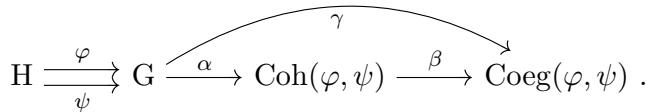
\includegraphics[keepaspectratio]{images/part002_030b7800.jpg}}

在本节（\(n^{o}\)）的余下部分，我们假设偶 \((\varphi,\psi)\) 的框架是一个连通箭图，并固定 G 的一个顶点 \(a_{0}\) 。于是，群胚 \(\mathrm{Coh}(\varphi,\psi)\) 与 \(\mathrm{Coeg}(\varphi,\psi)\) 都是传递的。

以 \(\Gamma\) 表示箭图 \((\mathrm{Som}(\mathrm{G}), \mathrm{Som}(\mathrm{H}), \mathrm{Som}(\varphi), \mathrm{Som}(\psi))\) ，以 \(\widetilde{\Gamma}\) 表示与 \(\Gamma\) 相伴的图，并设 \(\Omega(\widetilde{\Gamma})\) 为有限序列 \((z_1, \ldots, z_n)\) （\(\widetilde{\Gamma}\) 的箭组成的，其中 \(n \geqslant 1\) ）所成的集，这些序列满足：\(z_i\) 的靶是 \(z_{i+1}\) 的起点（若 \(1 \leqslant i < n\) ），且 \(z_n\) 的靶是 \(z_1\) 的起点。在第 1 号中我们构造了一个映射 \(\mathbf{z} \mapsto c(\mathbf{z})\) ，它从集 \(\Omega(\widetilde{\Gamma})\) 映入群 \(\mathrm{Coh}(\varphi, \psi)_{a_0}\) 的共轭类所成的集。

以 \(H \times_{G} H\) 表示 \(H \times H\) 中箭图态射 \(\psi \circ pr_{1}\) 与 \(\varphi \circ pr_{2}\) 的均衡子。其顶点集是 H 的顶点偶 \((a, b)\) （满足 \(\psi(a) = \varphi(b)\) ）所成的集；其箭集是 H 的箭偶 \((f, g)\) （满足 \(\psi(f) = \varphi(g)\) ）所成的集；箭 \((f, g)\) 的起点是顶点 \((o(f), o(g))\) ，其终点是顶点 \((t(f), t(g))\) （参看 II, 第 153 页）。

最后，以 \(\mathrm{Ker}(\varphi, \psi)\) 表示 \(\varphi\) 与 \(\psi\) 的均衡子；回忆（II, 第 165 页, 例 2），这是 H 的子箭图，其顶点 \(a\) 是满足 \(\varphi(a) = \psi(a)\) 的那些顶点，其箭是 \(f \in \mathrm{Fl}(\mathrm{H})\) （满足 \(\varphi(f) = \psi(f)\) ）所成的箭。

命题 4. —— 设 \(\mu\colon\mathrm{H}\times_{\mathrm{G}}\mathrm{H}\to\mathrm{H}\) 为满足 \(\varphi\circ\mu=\varphi\circ\mathrm{pr}_{1}\) 与 \(\psi\circ\mu=\psi\circ\mathrm{pr}_{2}\) 的一个箭图态射。假设：对 H 的每对顶点 \((a,b)\) （满足 \(\varphi(a)=\varphi(b)\) ），存在 H 的一个顶点 \(c\) ，使得 \(\varphi(c)=\psi(b)\) 且 \(a=\mu(b,c)\) 。

  设 \(A_{1}\) 为 \(\mathrm{Ker}(\varphi,\psi)\) 的、与其每个连通分支都相交的顶点集，并设 \(Z_{1}\) 为 \(\Omega(\widetilde{\Gamma})\) 中形如 \(((a,1))\) （其中 \(a\in A_{1}\) ）的元素所成的集。设 \(A_{2}\) 为与 \(H\times_{G}H\) 的每个连通分支都相交的 \(H\times_{G}H\) 的顶点集，并设 \(Z_{2}\) 为形如 \(((a,1),(b,1),(\mu(a,b),-1))\) （其中 \((a,b)\) 取遍 \(A_{2}\) ）的三元组所成的集。

那么，\(\Omega(\widetilde{\Gamma})\) 是 \(\Omega(\widetilde{\Gamma})\) 中包含 \(Z_1 \cup Z_2\) 的最小正规子集。特别地，共轭类 \(c(\mathbf{z})\) （在 \(\mathrm{Coh}(\varphi, \psi)_{a_0}\) 中，其中 \(\mathbf{z}\) 取遍 \(Z_1 \cup Z_2\) ）生成典范同态 \(\beta_{a_0}\) （从 \(\mathrm{Coh}(\varphi, \psi)_{a_0}\) 到 \(\mathrm{Coeg}(\varphi, \psi)_{\beta(a_0)}\) ）的核。

以 \(Z_{1}^{\prime}\) 、\(Z_{2}^{\prime}\) 与 \(Z^{\prime}\) 分别表示 \(\Omega(\widetilde{\Gamma})\) 中包含 \(Z_{1}\) 、\(Z_{2}\) 与 \(Z_{1} \cup Z_{2}\) 的最小正规子集（II, 第 197 页, 定义 1）。目标是证明 \(Z^{\prime}\) 等于 \(\Omega(\widetilde{\Gamma})\) 。由 II, 第 197 页的命题 1 的推论 1（II, 第 199 页），命题的后一断言将由此得出。

引理 1. —— a) 对每个顶点 \(a\) （\(\operatorname{Ker}(\varphi, \psi)\) 的），\(((a, 1))\) 属于 \(Z_1'\) 。

\begin{enumerate}
\def\labelenumi{\alph{enumi})}
\setcounter{enumi}{1}
\item
  对每个顶点 \((a,b)\) （\(\mathrm{H}\times_{\mathrm{G}}\mathrm{H}\) 的），\(((a,1),(b,1),(\mu(a,b),-1))\) 属于 \(\mathbf{Z}_2^{\prime}\) 。
\item
  设 \(A_{1}^{\prime}\) 为顶点 \(a\) （\(\operatorname{Ker}(\varphi,\psi)\) 的，使 \(((a,1))\) 属于 \(Z_{1}^{\prime}\) ）所成的集。我们有 \(A_{1}\subset A_{1}^{\prime}\) （根据 \(Z_{1}^{\prime}\) 的定义）。设 \(f\) 为 \(\operatorname{Ker}(\varphi,\psi)\) 的一条箭，\(a\) 为其起点，\(b\) 为其靶。把正规子集定义中的性质 (iv)（II, 第 197 页, 定义 1）应用于序列 \(((f,1))\) ，便得 \(a\in A_{1}^{\prime}\) 等价于 \(b\in A_{1}^{\prime}\) 。由于 \(A_{1}\) 与 \(\operatorname{Ker}(\varphi,\psi)\) 的每个连通分支相交，我们有 \(A_{1}^{\prime}=\operatorname{Som}(\operatorname{Ker}(\varphi,\psi))\) ，此即所要证明的。
\item
  设 \(A_{2}^{\prime}\) 为顶点 \((a,b)\) （\(H \times_{G} H\) 的，使三元组 \(((a,1),(b,1),(\mu(a,b),-1))\) 属于 \(Z_{2}^{\prime}\) ）所成的集。根据假设，有 \(A_{2} \subset A_{2}^{\prime}\) 。由于 \(A_{2}\) 与 \(H \times_{G} H\) 的每个连通分支相交，只需证明：若存在一条箭 \((f,f^{\prime})\) ，连接顶点 \((a', b')\) 与顶点 \((a, b)\) ，则 \((a, b)\) 属于 \(A_2'\) 当且仅当 \((a', b')\) 亦然。
\end{enumerate}

令 \(f'' = \mu(f, f')\) ；它是一条连接 \(\mu(a', b')\) 与 \(\mu(a, b)\) 的箭，且有 \(\varphi(f'') = \varphi(f)\) 与 \(\psi(f'') = \psi(f')\) 。把 \(\Omega(\widetilde{\Gamma})\) 的正规子集定义中的条件 (iv)（同前）应用于序列 \(((f, 1), (f', 1), (f'', -1))\) ，可知下列两个条件

\begin{enumerate}
\def\labelenumi{(\roman{enumi})}
\item
  三元组 \(((a,1),(b,1),(\mu (a,b), - 1))\) 属于 \(Z^{\prime}\) ；
\item
  三元组 \(((a',1),(b',1),(\mu(a',b'),-1))\) 属于 \(Z'\) 是等价的。这表明 \((a,b)\) 属于 \(A_{2}'\) 当且仅当 \((a',b')\) 属于 \(A_{2}'\) ，引理证明完毕。
\end{enumerate}

我们现在对整数 \(n \geqslant 1\) 作归纳来证明：每个元素 \(((a_1, \varepsilon_1), (a_2, \varepsilon_2), \ldots, (a_n, \varepsilon_n))\) （\(\Omega(\widetilde{\Gamma})\) 的）都属于 \(Z'\) 。

\casehead{\(n = 1\) 的情形}

设 \(((a,\varepsilon))\) 为 \(\Omega(\tilde{\Gamma})\) 的一个长度为 1 的元素。我们有 \(\varphi(a)=\psi(a)\) ，从而 \(((a,1))\in\mathbb{Z}'\)。由引理 1，正规子集定义中的条件 (ii) 进而蕴含 \(((a,-1))\) 属于 \(Z'\) 。

\casehead{\(n \geqslant 2\) 的情形}

根据正规子集的条件 (ii)，只需处理 \(\varepsilon_{2}=1\) 的情形。假设 \(\varepsilon_{1}=1\) ；那么 \((a_{1},a_{2})\) 是 H \(\times_{G}H\) 的一个顶点；令 \(a=\mu(a_{1},a_{2})\) ；由引理 1，三元组 \(((a_{1},1),(a_{2},1),(a,-1))\) 因此属于 \(Z'\)。在 \(\varepsilon_{1}=-1\) 的情形，我们有 \(\varphi(a_{1})=\varphi(a_{2})\) ；因此可以选取 H 的一个顶点 \(a\) ，使得 \(\mu(a_{2},a)=a_{1}\) ，且三元组 \(((a_{2},1),(a,1),(a_{1},-1))\) 属于 \(Z'\) ，于是根据正规子集定义中的条件 (ii)，三元组 \(((a_{1},-1),(a_{2},1),(a,1))\) 也属于 \(Z'\)。

于是，\(((a,\varepsilon_1),(a_3,\varepsilon_3),\ldots ,(a_n,\varepsilon_n))\) 属于 \(\Omega (\widetilde{\Gamma})\) 且长度为 \(n - 1\)。由归纳法，这是 \(\mathbf{Z}'\) 的一个元素。利用正规子集定义中的条件 (i)、(ii) 与 (iii)，我们相继推出下列元素

\[
\begin{array}{c} ((a _ {1}, \varepsilon_ {1}), (a _ {2}, 1), (a, - \varepsilon_ {1}), (a, \varepsilon_ {1}), (a _ {3}, \varepsilon_ {3}), \ldots , (a _ {n}, \varepsilon_ {n})), \\ ((a, - \varepsilon_ {1}), (a, \varepsilon_ {1}), (a _ {3}, \varepsilon_ {3}), \ldots , (a _ {n}, \varepsilon_ {n}), (a _ {1}, \varepsilon_ {1}), (a _ {2}, 1)), \\ ((a _ {3}, \varepsilon_ {3}), \ldots , (a _ {n}, \varepsilon_ {n}), (a _ {1}, \varepsilon_ {1}), (a _ {2}, 1)), \\ ((a _ {1}, \varepsilon_ {1}), (a _ {2}, 1), (a _ {3}, \varepsilon_ {3}), \ldots , (a _ {n}, \varepsilon_ {n})) \end{array}
\]

都属于 Z'。命题证明完毕。

推论. —— a) 采用命题 4 的记号，进一步假设从 Som(H) 映入 Som(G) × Som(G) 的映射 (Som(φ), Som(ψ)) 是单射的，且其像是 Som(G) 上一个等价关系的图。那么，对 H \(\times_{G}\) H 的每个顶点 (a, b)，存在唯一的 H 的顶点 \(c_{a,b}\) ，使得 \(\varphi(c_{a,b}) = \varphi(a)\) 且 \(\psi(c_{a,b}) = \psi(b)\) 。

\begin{enumerate}
\def\labelenumi{\alph{enumi})}
\setcounter{enumi}{1}
\tightlist
\item
  进一步假设：对每条箭 \((f, f')\) （H \(\times_{G}\) H 的），存在 H 的一条箭 \(f''\) ，使得 \(\varphi(f'') = \varphi(f)\) 且 \(\psi(f'') = \psi(f')\) 。
\end{enumerate}

设 A 为与 H \(\times_{G}\) H 的每个连通分支都相交的顶点集。那么，态射 \(\beta_{a_{0}}\) 的核是 \(\mathrm{Coh}(\varphi,\psi)_{a_{0}}\) 中包含共轭类 \(c((a,1),(b,1),(c_{a,b},-1))\) （对 \((a,b)\in\mathrm{A}\) ）的最小正规子群。

设 R 为 \(\operatorname{Som}(\mathrm{G})\) 上以映射 \((\operatorname{Som}(\varphi),\operatorname{Som}(\psi))\) 的像为图的等价关系。设 \((a,b)\) 为 \(H\times_{G}H\) 的一个顶点。于是有 \(\operatorname{R}\{\varphi(a),\psi(a)\}\) 与 \(\operatorname{R}\{\varphi(b),\psi(b)\}\) ，从而 \(\operatorname{R}\{\varphi(a),\psi(b)\}\) （因为 \(\psi(a)=\varphi(b)\) ）。因此，存在唯一的 H 的顶点 \(c\) ，使得 \(\varphi(c)=\varphi(a)\) 且 \(\psi(c)=\psi(b)\) ；把它记作 \(\mu(a,b)\) 。

对每条箭 \((f, f')\) （\(H\times_{G}H\) 的），选取 H 的一条箭 \(f''\) ，使得 \(\varphi(f'') = \varphi(f)\) 且 \(\psi(f'') = \psi(f')\) ，并把它记作 \(\mu(f, f')\) 。

我们就这样定义了一个箭图态射 \(\mu\colon\mathrm{H}\times_{\mathrm{G}}\mathrm{H}\to\mathrm{H}\) ，满足 \(\varphi\circ\mu=\varphi\circ\mathrm{pr}_{1}\) 与 \(\psi\circ\mu=\psi\circ\mathrm{pr}_{2}\) 。

设 \((a,b)\) 为满足 \(\varphi(a)=\varphi(b)\) 的一对 H 的顶点。我们有 \(\mathrm{R}\{\varphi(a),\psi(a)\}\) 与 \(\mathrm{R}\{\varphi(b),\psi(b)\}\) ，因此 \(\mathrm{R}\{\psi(b),\psi(a)\}\) 。从而存在唯一的 H 的顶点 \(c\) ，使得 \(\varphi(c)=\psi(b)\) 且 \(\psi(c)=\psi(a)\) 。顶点 \(\mu(b,c)\) 满足 \(\varphi(\mu(b,c))=\varphi(b)=\varphi(a)\) 与 \(\psi(\mu(b,c))=\psi(c)=\psi(a)\) 。 我们因此有 \(\mu(b,c)=a\) ，因为映射 \((\operatorname{Som}(\varphi),\operatorname{Som}(\psi))\) （从 \(\operatorname{Som}(\operatorname{H})\) 映入 \(\operatorname{Som}(\operatorname{G})\times\operatorname{Som}(\operatorname{G})\) ）是单射的。

设 \(A_{1}\) 为 \(\operatorname{Ker}(\varphi,\psi)\) 的顶点集，并设 \(Z_{1}\) 为 \(\Omega(\widetilde{\Gamma})\) 中形如 \(((a,1))\) （对 \(a\in A_{1}\) ）的元素所成的集。令 \(A_{2}=A\) ，并设 \(Z_{2}\) 为形如 \(((a,1),(b,1),(\mu(a,b),-1))\) 的元素（\(\Omega(\widetilde{\Gamma})\) 的，对 \((a,b)\in A_{2}\) ）所成的集。以 \(\widetilde{Z}\) （相应地 \(\widetilde{Z}_{1}\) ，或 \(\widetilde{Z}_{2}\)）表示 \(\Omega(\widetilde{\Gamma})\) 中包含 \(Z_{1}\cup Z_{2}\) （相应地 \(Z_{1}\) ，或 \(Z_{2}\)）的最小正规子集。

设 \(a \in \mathrm{A}_1\) 。我们有 \(\varphi(a) = \psi(a)\) ；令 \(x = \varphi(a)\)。顶点 \(a\) 是满足 \(\varphi(a) = \psi(a) = x\) 的 H 的唯一顶点。特别地，我们有 \(\mu(a, a) = a\)。因此三元组 \(((a, 1), (a, 1), (a, -1))\) 属于 \(\mathbf{Z}_2\)。进而由正规子集定义中的条件 (i) 与 (iii) 得出 \(((a, 1))\) 属于 \(\widetilde{\mathbf{Z}}_2\)。从而我们有 \(\mathbf{Z}_1 \subset \widetilde{\mathbf{Z}}_2\) ，于是 \(\widetilde{\mathbf{Z}} = \widetilde{\mathbf{Z}}_2\) 。

由命题 4，\(\Omega(\tilde{\Gamma})\) 是 \(\Omega(\tilde{\Gamma})\) 中包含 \(Z_{2}\) 的最小正规子集，且 \(\beta_{a_{0}}\) 的核是 \(\mathrm{Coh}(\varphi,\psi)_{a_{0}}\) 中包含共轭类 \(c(\mathbf{z})\) （对 \(\mathbf{z}\in Z_{2}\) ）的最小正规子群。推论得证。

例. —— 设 X 与 R 为拓扑空间，o 与 t 为从 R 到 X 的连续映射，C 为偶 \((f,g)\in\mathrm{R}^{2}\) （满足 \(t(f)=o(g)\) ）所成的集，m 为使箭图 \((\mathrm{X},\mathrm{R},o,t)\) 成为一个群胚的从 C 到 R 的连续映射；进一步假设从 R 到 R 的映射 \(f\mapsto f^{-1}\) 是连续的。若令 \(\mathrm{H}=\varpi(\mathrm{R})\) 、\(\mathrm{G}=\varpi(\mathrm{X})\) 、\(\varphi=\varpi(o)\) 、\(\psi=\varpi(t)\) 与 \(\mu=\varpi(m)\) ，则命题的假设得到满足。

进一步假设 R 是 X 上一个等价关系的图，其中映射 o 与 t 由 \(X \times X\) 到 X 的投影通过取子空间导出。于是推论的假设得到满足。

注记. —— *更一般地，当 (G, H, \(\varphi\) , \(\psi\) , \(\mu\) ) 是一个“群胚的群胚”时，命题的假设得到满足。这意味着 G 与 H 都是群胚，\(\varphi\) 与 \(\psi\) 是从 H 到 G 的群胚态射，使四元组 (G, H, \(\varphi\) , \(\psi\) ) 成为一个“群胚箭图”；最后，\(\mu\) 是这个“箭图”中由一个群胚态射 H \(\times_{\mathrm{G}}\) H → H 给出的合成法则，它满足表达该法则的结合性以及每条“箭”皆可逆的一定数目的性质。读者还会注意到，本书中所研究的基本群胚的应用全都属于这种情形。

\subsection{余均衡子的迷向群}

设 G 与 H 为群胚；设 \(\varphi\) 与 \(\psi\) 为从 H 到 G 的群胚态射。本节的目的在于总结上同伦子的迷向群的计算（II, 第 193 页, 命题 6）以及上一节中所作的上同伦子与余均衡子的迷向群的比较，以便由此推出余均衡子 Coeg( \(\varphi\) , \(\psi\) ) 的迷向群的计算。

以 \(\alpha\colon\mathrm{G}\to\mathrm{Coh}(\varphi,\psi)\) 、\(\beta\colon\mathrm{Coh}(\varphi,\psi)\to\mathrm{Coeg}(\varphi,\psi)\) 与 \(\gamma=\beta\circ\alpha\colon\mathrm{G}\to\mathrm{Coeg}(\varphi,\psi)\) 表示典范群胚态射。以 \(h\colon\mathrm{Som}(\mathrm{H})\to\mathrm{Fl}(\mathrm{Coh}(\varphi,\psi))\) 表示典范同伦；回忆 \(\mathrm{Coh}(\varphi,\psi)\) 的顶点集等于 \(\mathrm{Som}(\mathrm{G})\) 。

以 \(\Gamma\) 表示箭图 (Som(G), Som(H), Som(φ), Som(ψ))，再以 \(\varphi_0\) 与 \(\psi_0\) 表示由 \(\varphi\) 与 \(\psi\) 通过取轨道诱导的映射，以 \(\Gamma_0\) 表示 (Orb(G), Orb(H), \(\varphi_0, \psi_0\) ) ，即偶 ( \(\varphi, \psi\) ) 的框架。我们将假设箭图 \(\Gamma_0\) 是连通的且其顶点集非空，这等价于假设群胚 Coh(φ, ψ) 与 Coeg(φ, ψ) 都是传递的。

回忆（参看 II, 第 192 页, 定义 4），基本配备由下列数据组成：一个族 \((a, b, c_1, c_2, \mathrm{T}, i_0)\) ，其中：对所有 \(i \in \mathrm{Orb}(\mathrm{G})\) ，\(a(i)\) 是轨道 \(i\) （\(\mathrm{G}\) 的）中的一个顶点；对每个 \(j \in \mathrm{Orb}(\mathrm{H})\) ，\(b(j)\) 是轨道 \(j\) （\(\mathrm{H}\) 的）中的一个顶点，\(c_1(j)\) 与 \(c_2(j)\) 分别是 \(\mathrm{G}\) 中从 \(\varphi(b(j))\) 到 \(a(\varphi_0(j))\) 以及从 \(\psi(b(j))\) 到 \(a(\psi_0(j))\) 的箭；\(\mathrm{T}\) 是 \(\Gamma_0\) 的一个子箭图，其相伴树是图 \(\widetilde{\Gamma}_0\) 的一个极大树；最后，\(i_0\) 是 \(\mathrm{G}\) 的一个轨道，且我们令 \(a_0 = a(i_0)\) 。

我们随后定义一个箭图态射 \(\tau_0\) （从 \(\Gamma_0\) 到 \(\mathrm{Coh}(\varphi, \psi)\) ），使得 \(\tau_0(i) = \beta(a(i))\) 以及 \(\tau_0(j) = \alpha(c_1(j))^{-1}h(b(j))\alpha(c_2(j))\) （对 \(i \in \mathrm{Orb}(\mathrm{G})\) 及 \(j \in \mathrm{Orb}(\mathrm{H})\) ）。若 \(i\) 属于 \(\mathrm{Orb}(\mathrm{G})\) ，设 \(d_i\) 为图 \(\widetilde{\mathrm{T}}\) 中连接 \(i_0\) 与 \(i\) 的唯一的道路类，并以 \(\delta_i\) 表示它在 \(\mathrm{Coh}(\varphi, \psi)\) 中的、由群胚态射 \(\tau_0\) 给出的像。

由这些数据，II, 第 193 页的命题 6 给出一个满射同态。

\[
\Lambda \colon \bigl (\underset {i \in \pi_ {0} (\mathrm{G})} {*} \mathrm{G} _ {a (i)} \bigr) * \mathrm{F} (\operatorname{Orb} (\mathrm{H})) \to \operatorname{Coh} (\varphi , \psi) _ {a (i _ {0})}
\]

并描述其核的生成元，从而给出群 \(\mathrm{Coh}(\varphi,\psi)_{a_{0}}\) 的一个表现。

长度 \(\geqslant 1\) 的回路所成的集——在图 \(\widetilde{\Gamma}\) （与 \(\Gamma\) 相伴的）中——与集 \(\Omega(\widetilde{\Gamma})\) ——即序列 \((z_1, \ldots, z_n)\) （\(\widetilde{\Gamma}\) 的箭组成的，以 \(\mathbf{Z}/n\mathbf{Z}\) 为指标集）所成的集——等同，其中 \(n\) 取遍整数集 \(\geqslant 1\) ，且对每个 \(k \in \mathbf{Z}/n\mathbf{Z}\) ，\(z_k\) 的靶是 \(z_{k+1}\) 的起点。设 \(\mathbf{Z}\) 为 \(\Omega(\widetilde{\Gamma})\) 的一个子集，使共轭类 \(c(z)\) （对 \(z \in \mathbf{Z}\) ）生成满射同态 \(\beta_{a_0}\) 的核。同态 \(\beta_{a_0} \circ \Lambda\) 是满射的；为由此推出它的核，即群 \(\operatorname{Coeg}(\varphi, \psi)_{\beta(a_0)}\) 的一个表现，还需对每个 \(z \in \mathbf{Z}\) 选取一个元素 \(\mathrm{C}(z)\) （在群 \(\left( \begin{array}{cc} * & \mathrm{G}_{a(i)} \\ i \in \mathrm{Orb}(\mathrm{G}) & \end{array} \right) * \mathrm{F}(\pi_0(\mathrm{H}))\) 中），使 \(\Lambda(\mathrm{C}(z))\) 属于共轭类 \(c(z)\) 。

于是设 \(z = (z_{1}, \ldots, z_{n})\) 为 \(\Omega(\tilde{\Gamma})\) 的一个元素；令 \(z_{k} = (y_{k}, \varepsilon_{k})\) ，其中 \(y_{k} \in \mathrm{Fl}(\Gamma) = \mathrm{Som}(\mathrm{H})\) 且 \(\varepsilon_{k} \in \{\pm 1\}\) 。根据定义，\(c(z)\) 是元素的共轭类

\[
g h (y _ {1}) ^ {\varepsilon_ {1}} \dots h (y _ {n}) ^ {\varepsilon_ {n}} g ^ {- 1}
\]

的、在群 \(\mathrm{Coh}(\varphi,\psi)_{a_{0}}\) 中的共轭类，其中 g 是 \(\mathrm{Coh}(\varphi,\psi)\) 中连接 \(a_{0}\) 与 \(z_{1}\) 的起点的任意一条箭。对 \(k \in Z/nZ\) ，设 \(j_{k}\) 为 \(y_{k}\) 在 H 中的轨道，并选取 H 的一条箭 \(f_{k}\) ，它连接 \(y_{k}\) 与顶点 \(b(j_{k})\)。根据同伦的定义，我们随后有关系式

\[
h (y _ {k}) (\alpha \circ \psi) (f _ {k}) = (\alpha \circ \varphi) (f _ {k}) h (b (j _ {k}))
\]

在群胚 \(\mathrm{Coh}(\varphi,\psi)\) 中成立。于是，利用箭图态射 \(\tau_{0}\) 的定义，我们有

\[
\begin{array}{l} h (y _ {k}) = (\alpha \circ \varphi) (f _ {k}) \cdot h (b (j _ {k})) \cdot (\alpha \circ \psi) (f _ {k}) ^ {- 1} \\ \quad = (\alpha \circ \varphi) (f _ {k}) \cdot (\alpha \circ c _ {1}) (j _ {k}) \cdot \tau_ {0} (j _ {k}) \cdot (\alpha \circ c _ {2}) (j _ {k}) ^ {- 1} \cdot (\alpha \circ \psi) (f _ {k}) ^ {- 1} \\ \quad = (\alpha \circ \varphi) (f _ {k}) \cdot (\alpha \circ c _ {1}) (j _ {k}) \cdot \delta_ {\varphi_ {0} (j _ {k})} ^ {- 1} \cdot \\ \quad \cdot \delta_ {\varphi_ {0} (j _ {k})} \cdot \tau_ {0} (j _ {k}) \cdot \delta_ {\psi_ {0} (j _ {k})} ^ {- 1} \cdot \\ \quad \cdot \delta_ {\psi_ {0} (j _ {k})} \cdot (\alpha \circ c _ {2}) (j _ {k}) ^ {- 1} \cdot (\alpha \circ \psi) (f _ {k}) ^ {- 1} \\ = u _ {k} \Lambda (j _ {k}) v _ {k}, \end{array}
\]

其中我们已令

\[
u _ {k} = \alpha (\varphi (f _ {k}) c _ {1} (j _ {k})) \cdot \delta_ {\varphi_ {0} (j _ {k})} ^ {- 1} \quad \text { and } \quad v _ {k} = \delta_ {\psi_ {0} (j _ {k})} \cdot \alpha (\psi (f _ {k}) c _ {2} (j _ {k})) ^ {- 1}.
\]

对每个元素 \(k \in \mathbf{Z}/n\mathbf{Z}\) ，定义箭 \(\widetilde{u}_{k}, \widetilde{v}_{k}\) （G 中的）如下

\[
h (y _ {k}) ^ {\varepsilon_ {k}} = \widetilde {u} _ {k} \Lambda (j _ {k}) ^ {\varepsilon_ {k}} \widetilde {v} _ {k},
\]

使得

\[
(\widetilde {u} _ {k}, \widetilde {v} _ {k}) = \left\{ \begin{array}{l l} (u _ {k}, v _ {k}) & \text { if } \varepsilon_ {k} = 1; \\ (v _ {k} ^ {- 1}, u _ {k} ^ {- 1}) & \text { if } \varepsilon_ {k} = - 1. \end{array} \right.
\]

以 \(x_{k}\) 表示箭 \(h(y_{k})^{\varepsilon_{k}}\) 的起点；其靶则为 \(x_{k+1}\) ；设 \(i_{k}\) 为 \(x_{k}\) 的轨道。于是我们用下列公式定义群胚 G 中的回路 \(\lambda_{k}(z)\) （以 \(a(i_{k})\) 为基点的）：

\[
\lambda_ {k} (z) = \left\{ \begin{array}{l l} c _ {2} (j _ {k - 1}) ^ {- 1} \psi (f _ {k - 1}) ^ {- 1} \varphi (f _ {k}) c _ {1} (j _ {k}) & \text {if} (\varepsilon_ {k - 1}, \varepsilon_ {k}) = (1, 1); \\ c _ {2} (j _ {k - 1}) ^ {- 1} \psi (f _ {k - 1}) ^ {- 1} \psi (f _ {k}) c _ {2} (j _ {k}) & \text {if} (\varepsilon_ {k - 1}, \varepsilon_ {k}) = (1, - 1); \\ c _ {1} (j _ {k - 1}) ^ {- 1} \varphi (f _ {k - 1}) ^ {- 1} \varphi (f _ {k}) c _ {1} (j _ {k}) & \text {if} (\varepsilon_ {k - 1}, \varepsilon_ {k}) = (- 1, 1); \\ c _ {1} (j _ {k - 1}) ^ {- 1} \varphi (f _ {k - 1}) ^ {- 1} \psi (f _ {k}) c _ {2} (j _ {k}) & \text {if} (\varepsilon_ {k - 1}, \varepsilon_ {k}) = (- 1, - 1) \end{array} \right.\tag{1}
\]

根据构造，我们有

\[
\Lambda (\lambda_ {k} (z)) = \widetilde {v} _ {k - 1} \widetilde {u} _ {k},
\]

从而元素在同态 \(\Lambda\) 下的像

\[
\mathrm{C} (z) = \lambda_ {1} (z) (j _ {1}) ^ {\varepsilon_ {1}} \lambda_ {2} (z) (j _ {2}) ^ {\varepsilon_ {2}} \dots \lambda_ {n} (z) (j _ {n}) ^ {\varepsilon_ {n}}\tag{2}
\]

属于共轭类 \(c(z)\) 。

定义 3. —— 设 G 与 H 为群胚；设 \(\varphi\) 与 \(\psi\) 为从 H 到 G 的群胚态射。我们假设群胚 Coeg \((\varphi, \psi)\) 是传递的。设 \((a, b, c_1, c_2, T, i_0)\) 为偶 \((\varphi, \psi)\) 的一个基本配备。

我们称补配备为下列数据：一个子集 Z （\(\Omega(\widetilde{\Gamma})\) 的），使共轭类 \(c(\mathbf{z})\) （对 \(\mathbf{z} \in \mathbf{Z}\) ）生成同态 \(\beta_{a(i_0)}\) 的核；并且，对 Z 的每个元素 \(\mathbf{z} = ((y_1, \varepsilon_1), \ldots, (y_n, \varepsilon_n))\) ，给出箭的一个序列 \(f(\mathbf{z}) = (f_1, \ldots, f_n)\) （H 中的），使得 \(f_k\) 连接 \(y_k\) 与顶点 \(b(j_k)\) ，其中 \(j_k\) 表示 \(y_k\) 在 H 中的轨道。

偶 \((\varphi,\psi)\) 的一个完备配备是指一个基本配备与一个补配备的数据。

命题 5. —— 设 G 与 H 为群胚；设 \(\varphi\) 与 \(\psi\) 为从 H 到 G 的群胚态射。假设群胚 \(\operatorname{Coeg}(\varphi, \psi)\) 是传递的。以 \(\gamma\colon \mathrm{G} \to \mathrm{Coeg}(\varphi, \psi)\) 表示典范群胚态射。

我们给偶 \((\varphi, \psi)\) 配备一个完备配备

\[
(a, b, c _ {1}, c _ {2}, \mathrm{T}, i _ {0}, \mathrm{Z}, (f (\mathbf {z})) _ {\mathbf {z} \in \mathrm{Z}}).
\]

对 \(j \in \text{Orb(H)}\) ，设 \(\varphi_j \colon \text{H}_{b(j)} \to \text{G}_{a(\varphi_0(j))}\) 与 \(\psi_j \colon \text{H}_{b(j)} \to \text{G}_{a(\psi_0(j))}\) 分别为群同态 \(\text{Int}(c_1(j))^{-1} \circ \varphi_{b(j)}\) 与 \(\text{Int}(c_2(j))^{-1} \circ \psi_{b(j)}\) ，其中 \(\varphi_0\) 与 \(\psi_0\) 表示由 \(\varphi\) 与 \(\psi\) 通过取轨道诱导的典范映射。设 \(\tau\) 为框架 \(\Gamma_0\) （偶 \((\varphi, \psi)\) 的）到 \(\text{Coeg}(\varphi, \psi)\) 中的态射，由 \(\text{Som}(\tau)(i) = \gamma(a(i))\) （若 \(i \in \text{Orb(G)}\) ）定义，且使 \(\text{Fl}(\tau)(j)\) 是道路 \(\gamma(c_1(j))^{-1} \gamma(c_2(j))\) （在 \(\text{Coeg}(\varphi, \psi)\) 中的）。若 \(i\) 是 G 的一个轨道，设 \(c_i\) 为 \(\widetilde{\text{T}}\) 中连接 \(i_0\) 与 \(i\) 的唯一的道路类，并令 \(\delta_i = \widetilde{\tau}(c_i)\) ，其中 \(\widetilde{\tau} \colon \text{Grp(G)} \to \text{Coeg}(\varphi, \psi)\) 是由 \(\tau\) 诱导的典范群胚态射。

于是存在唯一的群同态

\[
\lambda \colon \bigl ( \begin{array}{c} * \\ i \in \operatorname{Orb} (\mathrm{G}) \end{array} \mathrm{G} _ {a (i)} \bigr) * \mathrm{F} (\operatorname{Orb} (\mathrm{H})) \to \operatorname{Coeg} (\varphi , \psi) _ {\gamma (a (i _ {0}))}
\]

使得

\[
\begin{array}{l l} \lambda (f) = \delta_ {i} \gamma_ {a (i)} (f) \delta_ {i} ^ {- 1} & \text { for } i \in \mathrm{Orb(G)} \text { and } f \in \mathrm{G} _ {a (i)}, \\ \lambda (j) = \delta_ {\varphi_ {0} (j)} \tau (j) \delta_ {\psi_ {0} (j)} ^ {- 1} & \text { for } j \in \mathrm{Orb(H)}. \end{array}
\]

同态 \(\lambda\) 是满射的；其核是包含下列元素的最小正规子群：

\[
\left(\mathrm{R} _ {1}\right) \quad r _ {1} (j) = j \quad \text { for } j \text { in } \mathrm{Fl} (\mathrm{T});
\]

\[
(\mathrm{R} _ {2}) \quad r _ {2} (j, f) = \varphi_ {j} (f) j \psi_ {j} (f) ^ {- 1} j ^ {- 1}
\]

\[
\text { for } j \in \operatorname{Orb} (\mathrm{H}) \text { and } f \in \mathrm{H} _ {b (j)};\tag{\((R_{3})\)}
\]

\[
r _ {3} (z) = \lambda_ {1} (z) j _ {1} ^ {\varepsilon_ {1}} \lambda_ {2} (z) j _ {2} ^ {\varepsilon_ {2}} \dots \lambda_ {n} (z) j _ {n} ^ {\varepsilon_ {n}}
\]

\[
\text { for } z = ((y _ {1}, \varepsilon_ {1}), \dots , (y _ {n}, \varepsilon_ {n})) \in \mathbf {Z},
\]

其中回路 \(\lambda_{i}(z)\) 由第 208 页的公式 (1) 定义。

这样一个态射的存在性与唯一性由群的族的自由积的泛性质得出（A, I, 第 85 页, 命题 8）。以 \(\alpha\colon G\to\mathrm{Coh}(\varphi,\psi)\) 与 \(\beta\colon\mathrm{Coh}(\varphi,\psi)\to\mathrm{Coeg}(\varphi,\psi)\) 表示典范态射，于是 \(\gamma=\beta\circ\alpha\)。再设 \(h\colon\mathrm{Som}(H)\to\mathrm{Fl}(\mathrm{Coh}(\varphi,\psi))\) 为联系 \(\alpha\circ\varphi\) 与 \(\alpha\circ\psi\) 的典范同伦。由于 \(\beta\) 是通过缩并 \(h\) 的像中的箭而得到的群胚态射，我们有

\[
\operatorname{Fl} (\tau) (j) = \gamma (c _ {1} (j)) ^ {- 1} \gamma (c _ {2} (j)) = \gamma (c _ {1} (j) ^ {- 1}) \beta (h (j)) \gamma (c _ {2} (j)) = \beta (\tau_ {0} (j))
\]

在 \(\operatorname{Coeg}(\varphi,\psi)\) 中成立，其中 \(\tau_{0}\colon\Gamma_{0}\to\mathrm{Coh}(\varphi,\psi)\) 表示由基本配备 \((a,b,c_{1},c_{2},\mathrm{T},i_{0})\) 诱导的箭图态射。于是，同态 \(\lambda\) 是命题 6（II, 第 193 页）中所定义的同态 \(\Lambda\) 与满射同态 \(\beta_{a(i_0)}\) 的复合。它特别是满射的。

设 \(z \in \mathbf{Z}\)。根据构造，\(\Lambda(r_3(z))\) 属于共轭类 \(c(z)\) 。根据补配备的定义，同态 \(\beta_{a(i_0)}\) 的核因此是 \(\mathrm{Coh}(\varphi, \psi)_{a(i_0)}\) 中包含元素 \(\Lambda(r_3(z))\) （对 \(z \in \mathbf{Z}\) ）的最小正规子群。由于同态 \(\Lambda\) 是满射的，同态 \(\lambda = \beta_{a(i_0)} \circ \Lambda\) 的核因此是群 \(\left( *_{i \in \mathrm{Orb}(G)} G_{a(i)} \right) * F(\pi_0(H))\) 中包含 \(\Lambda\) 的核的、由公式 \((R_1), (R_2)\) 给出的生成元以及由公式 \((R_3)\) 定义的元素的最小正规子群。命题得证。

\subsection{群胚被群作用的商}

设 G 为一个传递群胚，K 为一个群，并设 \(\theta\colon\mathrm{K}\to\mathrm{Aut}(\mathrm{G})^{\circ}\) 为从 K 到群胚 G 的自同构群之相反群中的群同态。我们将说群 K 右作用于 G。若 \(k\in\mathrm{K}\) ，我们有时以 \(k^{*}x\) （相应地 \(k^{*}f\) ）表示 G 的顶点 \(x\) （相应地箭 \(f\) ）在群胚自同构 \(\theta(k)\) 下的像。

设 \(|\mathrm{K}|\) 为这样的群胚：其顶点集为 \(\mathrm{K}\) ，连接两个顶点的箭集当这两个顶点不同时为空集，否则缩为单个元素。设 \(\mathrm{H}\) 为积群胚 \(\mathrm{G} \times |\mathrm{K}|\) ；\(\mathrm{H}\) 的一个顶点是偶 \((a,k)\) ，其中 \(a\) 是 \(\mathrm{G}\) 的一个顶点，\(k\) 是 \(\mathrm{K}\) 的一个元素；若 \(f\) 是 \(\mathrm{G}\) 中连接顶点 \(a\) 与顶点 \(b\) 的一条箭，我们以 \((f,k)\) 表示 \(\mathrm{H}\) 中连接 \((a,k)\) 与 \((b,k)\) 的唯一的箭。设 \(\varphi: \mathrm{H} \to \mathrm{G}\) 为由第一个投影给出的群胚态射，并设 \(\psi: \mathrm{H} \to \mathrm{G}\) 为满足 \(\operatorname{Som}(\psi)((a,k)) = k^*a\) 与 \(\operatorname{Fl}(\psi)((f,k)) = k^*f\) （若 \(k \in \mathrm{K}\) 、\(a \in \operatorname{Som}(\mathrm{G})\) 且 \(f \in \operatorname{Fl}(\mathrm{G})\) ）的群胚态射。

以 G/K 表示余均衡子 \(\operatorname{Coeg}(\varphi,\psi)\) ，并以 \(\gamma\colon G\to G/K\) 表示典范群胚态射。

设 o 为 G 的一个顶点。对 \(k \in K\) ，选取 G 中的一条箭 \(c_{k}\) （连接 \(k^{*}o\) 与 o 的）；由于 G 是传递的，这样的箭存在。对 \(k \in K\) ，以 \(\text{Fix}(k)\) 表示 G 的子群胚，其顶点（相应地箭）是被 k 固定的 \(\text{Som}(G)\) （相应地 \(\text{Fl}(G)\) ）的元素；我们选取一个顶点集 \(A_{k}\) （\(\text{Fix}(k)\) 的，与此群胚的所有轨道都相交）。对 \(k \in K\) 及 \(a \in A_{k}\) ，我们还选取 G 中连接顶点 a 与顶点 o 的一条箭 \(f_{(a,k)}\) 。

命题 6. —— 唯一的群同态

\[
\lambda \colon \mathrm{G} _ {o} * \mathrm{F} (\mathrm{K}) \to (\mathrm{G} / \mathrm{K}) _ {\gamma (o)}
\]

使得 \(\lambda(f) = \gamma_o(f)\) （对 \(f \in \mathrm{G}_o\) ）以及 \(\lambda([k]) = \gamma(c_k)\) （对 \(k \in \mathrm{K}\) ）者是满射的。其核是 \(\mathrm{G}_o * \mathrm{F}(\mathrm{K})\) 中包含下列元素的最小正规子群：

\[
r _ {2} (k, f) = [ k ] ^ {- 1} f [ k ] (c _ {k} ^ {- 1} k ^ {*} (f) ^ {- 1} c _ {k})\tag{\((R_{2})\)}
\]

\[
\text { for } k \in \mathrm{K} \text { and } f \in \mathrm{G} _ {o};\tag{\((\mathrm{R}_{3}^{\prime})\)}
\]

\[
r _ {3} ^ {\prime} (k, a) = [ k ] (c _ {k} ^ {- 1} k ^ {*} (f _ {(a, k)}) ^ {- 1} f _ {(a, k)}))
\]

\[
\text { for } k \in \mathrm{K} - \{e \} \text { and } a \in \mathrm{A} _{k}\tag{\((\mathrm{R}_{3}^{\prime\prime})\)}
\]

\[
r _ {3} ^ {\prime \prime} (k, h) = [ k h ] ^ {- 1} [ k ] [ h ] (c _ {h} ^ {- 1} h ^ {*} (c _ {k} ^ {- 1}) c _ {k h})
\]

\[
\text { for } k,h \in \mathrm{K}.
\]

由于 G 是传递的，把元素 \(k \in K\) 对应到 \((o, k)\) 的轨道的映射是 K 到 H 的轨道集上的一个双射。我们于是把 \(\operatorname{Orb}(\mathbf{G})\) 与 \(\{o\}\) 等同，把 \(\operatorname{Orb}(\mathbf{H})\) 与 K 等同。框架 \(\Gamma_{0}\) （偶 \((\varphi, \psi)\) 的）于是等同于具有单个顶点 o 且箭集为 K 的箭图。设 T 为 \(\Gamma_{0}\) 的、顶点集为 \(\{o\}\) 而箭集为空的子箭图；其相伴图是图 \(\widetilde{\Gamma}_{0}\) 的唯一的极大树。

族 \((o,(o,k)_{k\in \mathrm{K}},(e_o)_{k\in \mathrm{K}},(c_k)_{k\in \mathrm{K}},\mathrm{T},o)\) 是偶 \((\varphi ,\psi)\) 的一个基本配备。

映射 \(f \mapsto (f, k)\) 定义了迷向群 \(G_o\) 到迷向群 \(H_{(o,k)}\) 上的一个同构；在此同构下，同态 \(\varphi_k\) 与 \(\psi_k\) （从 \(H_{(o,k)}\) 到 \(G_o\) 中的、由 II, 第 208 页的命题 5 定义的）由下式给出

\[
\varphi_ {k} (f, k) = f \quad \text { and } \quad \psi_ {k} (f, k) = c _ {k} ^ {- 1} k ^ {*} (f) c _ {k},\tag{3}
\]

（对 \(k\in \mathrm{K}\) 及 \(f\in \mathrm{G}_o\) ）。

箭图 \(H \times_{G} H\) 是 \(H \times H\) 中箭图态射 \(\psi \circ pr_{1}\) 与 \(\varphi \circ pr_{2}\) 的均衡子。其顶点是偶 \(((a, k), (b, h))\) ，其中 a 与 b 是 G 的顶点，k 与 h 是 K 中满足 \(b = k^{*}a\) 的元素；其箭是偶 \(((f, k), (g, h))\) ，其中 f 与 g 是 G 的箭，k 与 h 是 K 中满足 \(g = k^{*}f\) 的元素；箭 \(((f,k),(g,h))\) 的起点等于 \(((o(f),k),(o(g),h))\) ；其靶等于 \(((t(f),k),(t(g),h))\) 。

我们随后定义一个箭图态射 \(\mu\) （从 \(H \times_{\mathrm{G}} H\) 到 H 中的），令 \(\mu((a,k),(b,h)) = (a,kh)\) 与 \(\mu((f,k),(g,h)) = (f,kh)\) 。我们有 \(\varphi \circ \mu = \varphi \circ \mathrm{pr}_1\) 与 \(\psi \circ \mu = \psi \circ \mathrm{pr}_2\) 。

设 \(x\) 与 \(y\) 为 H 中满足 \(\varphi(x) = \varphi(y)\) 的顶点。于是存在 G 的一个顶点 \(a\) 以及 K 的元素 \(k\) 与 \(h\) ，使得 \(x = (a, k)\) 且 \(y = (a, h)\) 。令 \(z = (h^* a, h^{-1} k)\) ；我们有 \(\mu(y, z) = x\)。这表明偶 \((\varphi, \psi)\) 满足 II, 第 202 页的命题 4 的假设。

H 的顶点 \((a,k)\) 属于群胚 \(\operatorname{Ker}(\varphi,\psi)\) （\(\varphi\) 与 \(\psi\) 的均衡子）当且仅当 \(k^{*}a=a\) ，即 k 属于群 K 中顶点 a 的稳定子。设 \(A_{1}\) 为偶 \((a,k)\) （对 \(k\in K\) 与 \(a\in A_{k}\)）所成的集；它与 H 的子群胚 \(\operatorname{Ker}(\varphi,\psi)\) 的所有轨道相交。设 \(Z_{1}\) 为 \(\Omega(\widetilde{\Gamma})\) 中由形如 (((a,k),1)) （对 \((a,k)\in A_{1}\)）的序列组成的部分。对 \(\mathbf{z}=((a,k),1)\in\mathbf{Z}_{1}\) ，\((f_{(a,k)},k)\) 是 H 的一条箭，它连接 \((a,k)\) 与 \((o,k)\) 。令 \(f(\mathbf{z})=((f_{(a,k)},k))\)。

顶点所成的集 \(\mathrm{A}_2\) （\(\mathrm{H} \times_{\mathrm{G}} \mathrm{H}\) 的，由形如 \(((o,k), (k^*o,h))\) （对 \((k,h) \in \mathrm{K}^2\) ）的顶点组成）与 \(\mathrm{H} \times_{\mathrm{G}} \mathrm{H}\) 的每个轨道相交。还可注意到 \(\mu((o,k), (k^*o,h)) = (o,kh)\) 。H 中的箭 \((e_o,k), (c_k,h), (e_o,kh)\) 分别连接 \((o,k), (k^*o,h), (o,kh)\) 到 \((o,k), (o,h)\) 与 \((o,kh)\) 。以 \(\mathrm{Z}_2\) 表示形如 \((((o,k),1), ((k^*o,h), 1), ((o,kh), -1))\) 的序列在 \(\Omega(\widetilde{\Gamma})\) 中所成的集；对这样一个元素 \(\mathbf{z}\) （\(\mathrm{Z}_2\) 的），令 \(f(\mathbf{z}) = ((e_o,k), (c_k,h), (e_o,kh))\) 。

由 II, 第 202 页的命题 4，集 \(Z = Z_1 \cup Z_2\) 与族 \((f(\mathbf{z}))_{z \in \mathbb{Z}}\) 构成一个补配备。

设 \(k \in \mathrm{K}\) 且 \(a \in \mathrm{A}_k\) 。元素 \(\mathrm{C}((a, k), 1)\) （由 II, 第 208 页的公式 (2) 定义的、群 \(\mathrm{G}_o * \mathrm{F}(\mathrm{K})\) 中的）等于

\[
c _ {k} ^ {- 1} \psi ((f _ {(a, k)}, k)) ^ {- 1} \varphi (f _ {(a, k)}) e _ {o} [ k ] = (c _ {k} ^ {- 1} k ^ {*} (f _ {(a, k)}) ^ {- 1} f _ {(a, k)}) [ k ].\tag{4}
\]

设 \(k,h \in \mathbf{K}\)。我们验证，元素

\[
\mathrm{C} (((o, k), 1), ((k ^ {*} o, h), 1), ((o, k h), - 1))
\]

（由 II, 第 208 页的公式 (2) 定义的、群 \(G_{o} * F(K)\) 中的）等于

\[
[ k ] [ h ] (c _ {h} ^ {- 1} h ^ {*} (c _ {k} ^ {- 1}) c _ {k h}) [ k h ] ^ {- 1}.\tag{5}
\]

元素 \(r_3'(e, a)\) （由关系式 \((\mathrm{R}_3')\) 对 \(k = e\) 给出的）都等于 \([e]c_e^{-1}\) ，后者是群 \(\mathrm{G}_o * \mathrm{F}(\mathrm{K})\) 中把关系式 \((\mathrm{R}_{3}^{\prime\prime})\) 应用于 \(k = h = e\) 而得到的元素。鉴于关系式 (3)、(4) 与 (5)，命题于是由 II, 第 208 页, 命题 5 得出。

推论 1. —— 假设群 K 由 G 的顶点的固定子生成。那么群同态 \(\gamma_{o}\colon\mathrm{G}_{o}\to(\mathrm{G}/\mathrm{K})_{\gamma(o)}\) 是满射的。此外，若群胚 G 是单传递的，则群胚 G/K 亦然。

关系式 \((\mathrm{R}_{3}^{\prime\prime})\) 蕴含 \(\lambda([e]) = \lambda(c_{e}) = \gamma_{o}(c_{e})\) 。关系式 \((\mathrm{R}_{3}^{\prime\prime})\) 进而蕴含：那些 \(k \in K\) （满足 \(\lambda([k])\) 属于 \(\gamma_{o}\) 的像的）组成 K 的一个子群。最后，关系式 \((\mathrm{R}_{3}^{\prime})\) 表明，对每个固定子非空的元素 \(k \in K\) ，\(\lambda([k])\) 属于 \(\gamma_{o}\) 的像。推论由此得出。

注记 1. —— 我们可以给出群 \((\mathrm{G}/\mathrm{K})_{\gamma(o)}\) 的另一个有时更方便的描述。为此，令 \(M = K \times G_{o}\) ，并用下列公式在 M 上定义一个合成法则

\[
(k, a) \cdot (h, b) = (k h, c _ {k h} ^ {- 1} h ^ {*} (c _ {k} a) c _ {h} b),
\]

（对 \(k\) 、\(h \in \mathrm{K}\) 及 \(a\) 、\(b \in \mathrm{G}_o\) ）。我们验证这个合成法则是结合的，\((e, c_e^{-1})\) 是一个恒等元，且元素 \((k^{-1}, c_{k^{-1}}^{-1}(k^{-1})^*(c_k a)^{-1} c_e)\) 是 \((k, a)\) 的逆。因此它赋予 M 一个群结构。此外，映射 \(\lambda'\colon \mathrm{M} \to (\mathrm{G} / \mathrm{K})_{\gamma(o)}\) （由 \((k, a) \mapsto \lambda([k]a)\) 定义的）是一个群同态。设 \(\alpha'\) 为从 \(\mathrm{G}_o * \mathrm{F}(\mathrm{K})\) 到 M 的唯一的群同态，满足 \(\alpha'(f) = (e, f)\) （若 \(f \in \mathrm{G}_o\) ）及 \(\alpha'([k]) = (k, e_o)\) （若 \(k \in \mathrm{K}\) ）；我们有 \(\lambda' \circ \alpha' = \lambda\) 。

关系式 \((\mathrm{R}_{2})\) 与 \((\mathrm{R}_{3}^{\prime\prime})\) 表明，\((\mathrm{G}/\mathrm{K})_{\gamma(o)}\) 的每个元素都是同态 \(\lambda\) 下、\(\mathrm{G}_{o}*\mathrm{F}(\mathrm{K})\) 中形如 \([k]f\) 的元素的像，其中 \(f\in G_{o}\) 且 \(k\in K\) 。因此，同态 \(\lambda'\) 是满射的。我们同样验证：\(\alpha'\) 下、\(\mathrm{G}_{o}*\mathrm{F}(\mathrm{K})\) 中形如 \((\mathrm{R}_{2})\) 或 \((\mathrm{R}_{3}^{\prime\prime})\) 的元素的像为零。于是，同态 \(\lambda'\) 的核是 M 的、包含 \(\alpha'\) 下 \(\mathrm{G}_{o}*\mathrm{F}(\mathrm{K})\) 中形如 \((\mathrm{R}_{3}^{\prime})\) 的元素的像的最小正规子群。

推论 2. —— 假设群 K 自由地作用于 Som(G)。那么存在唯一的群同态 \(\pi\colon (\mathrm{G} / \mathrm{K})_{\gamma (o)}\to \mathrm{K}\) ，其核包含 \(\gamma_{o}\) 的像，且满足 \(\pi (\lambda ([k])) = k\) （对所有 \(k\in \mathbf{K}\) ）。此外，\(\mathrm{G}_o\xrightarrow{\gamma_o} (\mathrm{G} / \mathrm{K})_{\gamma (o)}\xrightarrow{\pi}\mathrm{K}\) 是 K 被 \(\mathrm{G}_o\) 的一个扩张。

若这样一个群同态 \(\pi\) 存在，则群同态 \(\pi \circ \lambda\) 必然等于唯一的群同态 \(p\) （从 \(\mathrm{G}_{o} * \mathrm{F}(\mathrm{K})\) 到 \(\mathrm{K}\) 中的），满足 \(p(f) = e\) （对 \(f \in \mathrm{G}_{o}\) ）与 \(p([k]) = k\) 。立即可验证，\(\mathrm{G}_{o} * \mathrm{F}(\mathrm{K})\) 的、由公式 \((\mathrm{R}_{2})\) 与 \((\mathrm{R}_{3}^{\prime \prime})\) 定义的元素属于 \(p\) 的核。根据假设，不存在 \((\mathrm{R}_{3}^{\prime})\) 型的元素。于是，态射 \(\lambda\) 的核包含 \(p\) 的核。因此，存在唯一的群同态 \(\pi: (\mathrm{G} / \mathrm{K})_{\gamma(o)} \to \mathrm{K}\) ，使得 \(\pi \circ \lambda = p\) 。

显然同态 \(\pi\) 是满射的。为证明同态 \(\gamma_{o}\) 是单射的且其像恰为 \(\pi\) 的核，我们注意到同态 \(\lambda'\colon M \to (\mathrm{G}/\mathrm{K})_{\gamma(o)}\) （II, 第 213 页, 注记 1）是一个同构，因为我们已假设 K 自由地作用于 \(\operatorname{Som}(\mathrm{G})\)。复合同态 \((\lambda')^{-1} \circ \gamma_{o}\) （从 \(\mathrm{G}_{o}\) 到 M 中的）由 \(f \mapsto (e, f)\) 给出，而同态 \(\pi \circ \lambda'\colon M \to K\) 把 \((k, f)\) 映为 \(k\)。推论由此得出。

推论 3. —— 假设群胚 G 是单传递的。设 K₀ 为由 G 的顶点的稳定子生成的 K 的子群。从 K 到 \((\mathrm{G}/\mathrm{K})_{\gamma(o)}\) 的、把 \(k\) 映为 \(\gamma(c_k)\) 的映射是一个满射群同态，其核为 K₀。

若一个元素 \(k \in \mathrm{K}\) 固定顶点 \(a\) （\(\mathrm{G}\) 的），则元素 \(g^{-1}kg\) 固定顶点 \(g^{*}a\) ；这蕴含 \(\mathrm{K}_{0}\) 是 \(\mathrm{K}\) 的一个正规子群。

由命题 5，唯一的同态 \(\lambda\colon\mathrm{F}(\mathrm{K})\to(\mathrm{G}/\mathrm{K})_{\gamma(o)}\) （满足 \(\lambda([k])=\gamma(c_k)\) 的）是满射的，且其核是 F(K) 中包含元素 \([k]\) （其中 \(k\) 是固定 G 的一个顶点的、K 的元素）以及元素 \([kh]^{-1}[k][h]\) （其中 \((k,h)\in\mathrm{K}^2\) ）的最小正规子群。特别地，映射 \(\lambda'\colon\mathrm{K}\to(\mathrm{G}/\mathrm{K})_{\gamma(o)}\) （由 \(\lambda'(k)=\gamma(c_k)=\lambda([k])\) 对 \(k\in\mathrm{K}\) 定义的）是一个群同态。我们有 \(\lambda=\lambda'\circ p\) ，其中 \(p\colon\mathrm{F}(\mathrm{K})\to\mathrm{K}\) 表示典范满射群同态。因此，同态 \(\lambda'\) 是满射的，且其核是 K 中包含元素 \(k\) （对固定 G 的一个顶点的 \(k\) ）的最小正规子群，即 \(\mathrm{K}_0\)。命题得证。

\exerciseshdr{习题}

\exercisegroup

\begin{enumerate}
\def\labelenumi{\arabic{enumi})}
\tightlist
\item
  设 \((\mathrm{Q}_{i})_{i\in\mathrm{I}}\) 是一族箭图。用 S 表示族 \((\mathrm{Som}(\mathrm{Q}_{i}))\) 的和集，用 F 表示族 \((\mathrm{Fl}(\mathrm{Q}_{i}))\) 的和集，并用 o 与 t 表示由诸箭图 \(Q_{i}\) 的起点映射与终点映射诱导的从 F 到 S 的映射。
\end{enumerate}

\begin{enumerate}
\def\labelenumi{\alph{enumi})}
\item
  证明 \(\mathrm{Q} = (\mathrm{S}, \mathrm{F}, o, t)\) 是一个箭图。称它为族 \((\mathrm{Q}_{i})\) 的和箭图。
\item
  对 \(i \in I\)，存在唯一的箭图态射 \(j_{i}\)（由 \(Q_{i}\) 到 Q），使得映射 \(\operatorname{Som}(j_{i})\) 是从 \(\operatorname{Som}(Q_{i})\) 到 S 中的典范映射，且映射 \(\operatorname{Fl}(j_{i})\) 是从 \(\operatorname{Fl}(Q_{i})\) 到 S 中的典范映射。
\item
  设 K 是一个箭图，且对每个 \(i \in I\)，设 \(\varphi_{i}\) 是从 \(Q_{i}\) 到 K 的箭图态射。证明存在唯一的从 Q 到 K 的箭图态射 \(\varphi\)，使得 \(\varphi \circ j_{i} = \varphi_{i}\) 对所有 \(i \in I\) 成立。
\end{enumerate}

\begin{enumerate}
\def\labelenumi{\arabic{enumi})}
\setcounter{enumi}{1}
\tightlist
\item
  设 \(Q = (S, F, o, t)\) 是一个箭图。对每个 \(s \in S\)，称 \(d_{+}(s)\)（相应地，\(d_{-}(s)\)）为 Q 在 s 处的出次数（相应地，入次数），并把 \(d_{+}(s)\)（相应地，\(d_{-}(s)\)）定义为集合 \(\{f \in F \mid o(f) = s\}\)（相应地，\(\{f \in F \mid t(f) = s\}\)）的基数。若 \(d_{+}(s)\) 与 \(d_{-}(s)\) 对每个 \(s \in S\) 均有限，则称 Q 是局部有限的；若集合 F 与 S 均有限，则称 Q 是有限的。
\end{enumerate}

证明等式 \(\sum_{s\in S}d_{+}(s) = \sum_{s\in S}d_{-}(s) = \mathrm{Card}(\mathrm{F})\)

\begin{enumerate}
\def\labelenumi{\arabic{enumi})}
\setcounter{enumi}{2}
\tightlist
\item
  设 \(\mathrm{Q} = (\mathrm{S},\mathrm{F},o,t)\) 是一个局部有限箭图。我们定义矩阵 \(M_{\mathrm{Q}} = (m_{i,j})\)（类型为 (S,S)，元素在 \(\mathbf{Z}\) 中）如下：
\end{enumerate}

\[
 m _ {i, j} = \operatorname{Card} \left\{f \in \mathrm{F} \mid o (f) = i \text {and} t (f) = j \right\}.
\]

矩阵 \(M_{\mathrm{Q}}\) 称为 Q 的邻接矩阵。

\begin{enumerate}
\def\labelenumi{\alph{enumi})}
\item
  给定箭图 Q 与 Q'，给出关于它们的邻接矩阵的一个必要充分条件，使 Q 与 Q' 同构。
\item
  用邻接矩阵 \(M_{Q}\) 表出 Q 中起点与终点给定的长为 n 的道路的数目。
\item
  证明一个图的底箭图的邻接矩阵是对称的。
\end{enumerate}

\begin{enumerate}
\def\labelenumi{\arabic{enumi})}
\setcounter{enumi}{3}
\tightlist
\item
  设 \(Q = (S, F, o, t)\) 是一个箭图。用 I 表示族 \((S, F)\) 的和集；把 S 与 F 等同于 I 的子集。设 k 是一个交换环。把箭图 Q 的 k-代数称为商 \(A_{Q}\)（即集合 I 上的自由结合 k-代数对由元素 \(X_{s}^{2} - X_{s}\)（对 \(s \in S\)）、\(X_{u}X_{v} - X_{v}X_{u}\)（对 \(u, v \in S\)）、\(X_{f}X_{t(f)} - X_{f}\) 与 \(X_{o(f)}X_{f} - X_{f}\)（对 \(f \in F\)）所生成的双边理想所作的商）。对 \(i \in I\)，用 \(x_{i}\) 表示 \(X_{i}\) 在代数 \(A_{Q}\) 中的像。
\end{enumerate}

\begin{enumerate}
\def\labelenumi{\alph{enumi})}
\item
  证明有 \(\sum_{s\in S}x_s = 1\)
\item
  证明若 f 与 g 是 Q 中不可合成的箭，则有 \(x_{f}x_{g}=0\)。
\item
  对 Q 中每条道路 \(c = (a_{0}, f_{1}, \ldots, f_{n}, a_{n})\)，令 \(x_{c} = x_{a_{0}} x_{f_{1}} \ldots x_{f_{n}}\)。设 c 与 \(c'\) 是 Q 中的道路；证明有 \(x_{c} x_{c'} = x_{cc'}\)（若 c 与 \(c'\) 可合成），否则有 \(x_{c} = x_{c'}\)。
\item
  设 C 是箭图 Q 中道路的集合；证明族 \((x_{c})_{c\in C}\) 是 k-模 \(A_{Q}\) 的一组基。
\item
  设 \(J_{Q}\) 是 \(A_{Q}\) 中由形如 \(x_{f}\)（\(f \in F\)）的元素生成的双边理想。证明代数 \(A_{Q}/J_{Q}\) 同构于 \(k^{(S)}\)。
\item
  为使 k-代数 \(A_{Q}\) 是一个有限生成的 k-模，必要且充分的是 Q 的顶点集有限且 Q 中每个圈的长为零。此时理想 \(J_{Q}\) 是幂零的。
\end{enumerate}

在 §1 的其余习题中，我们沿用这些记号。当我们说到 \(A_{Q}\)-模（不作另外说明时），指的是右模。若 A 是一个环，A-模 M（不作另外说明时）总指右 A-模；若 a 是 A 的一个元素，用 \(a_{M}\) 或 \((a)_{M}\) 表示 M 的位似 \(x \mapsto xa\)。

\begin{enumerate}
\def\labelenumi{\arabic{enumi})}
\setcounter{enumi}{4}
\tightlist
\item
  \begin{enumerate}
  \def\labelenumii{\alph{enumii})}
  \tightlist
  \item
    证明四元组 \(Q^{\circ} = (S, F, t, o)\) 是一个箭图。称它为 Q 的反箭图。
  \end{enumerate}
\end{enumerate}

\begin{enumerate}
\def\labelenumi{\alph{enumi})}
\setcounter{enumi}{1}
\tightlist
\item
  代数 \(A_{Q^{\circ}}\) 同构于代数 \(A_{Q}\) 的反代数。
\end{enumerate}

\begin{enumerate}
\def\labelenumi{\arabic{enumi})}
\setcounter{enumi}{5}
\tightlist
\item
  \begin{enumerate}
  \def\labelenumii{\alph{enumii})}
  \tightlist
  \item
    设 \((M_s)_{s\in\operatorname{Som}(Q)}\) 是一族 \(k\)-模，\((u_f)_{f\in\operatorname{Fl}(Q)}\) 是一个族，其中对每个 \(f\in\operatorname{Fl}(Q)\)，\(u_f\) 是从 \(M_{o(f)}\) 到 \(M_{t(f)}\) 的线性映射。设 M 是族 \((M_s)\) 的直和；对 \(s\in S\)，用 \(j_s\) 表示 \(M_s\) 到 M 中的典范单射，用 \(p_s\) 表示 M 到 \(M_s\) 上的典范投影。证明在 M 上存在唯一的 \(A_Q\)-模结构，使得有 \((x_s)_M = j_s \circ p_s\) 且 \((x_f)_M = j_{t(f)} \circ u_f \circ p_{o(f)}\)（对所有 \(s \in \operatorname{Som}(Q)\) 及每个 \(f \in \operatorname{Fl}(Q)\)）。
  \end{enumerate}
\end{enumerate}

反之，每个 \(A_{Q}\)-模都具有此形式。

\begin{enumerate}
\def\labelenumi{\alph{enumi})}
\setcounter{enumi}{1}
\tightlist
\item
  若 \(\Lambda\) 是一个 \(k\)-模且 \(s \in \operatorname{Som}(\mathbf{Q})\)，用 \(\Lambda(s)\) 表示如下的 \(\mathrm{A}_{\mathrm{Q}}\)-模：它与族 \((\mathrm{M}_i)_{i \in \operatorname{Som}(\mathbf{Q})}\)（一个 \(k\)-模族，由 \(\mathrm{M}_i = \Lambda\)（若 \(i = s\)）、否则 \(\mathrm{M}_i = 0\) 给出）以及线性映射族 \((u_f)_{f \in \operatorname{Fl}(\mathbf{Q})}\)（其中 \(u_f = 0\) 对一切 \(f \in \operatorname{Fl}(\mathbf{Q})\)）相伴。
\end{enumerate}

设 \(\Lambda\) 与 \(\Lambda'\) 是非零 \(k\)-模。设 \(s\) 与 \(s'\) 是 Q 的顶点。证明 \(\Lambda(s)\) 同构于 \(\Lambda'(s')\) 当且仅当 \(\Lambda\) 与 \(\Lambda'\) 作为 \(k\)-模同构且 \(s = s'\)。

\begin{enumerate}
\def\labelenumi{\alph{enumi})}
\setcounter{enumi}{2}
\item
  若 \(\Lambda\) 是一个单 \(k\)-模，则 \(\Lambda(s)\) 都是单 \(\mathrm{A}_{\mathrm{Q}}\)-模（对每个顶点 \(s\)）。
\item
  进一步假设 Q 中每个圈的长为零。证明每个单 \(A_Q\)-模都具有形式 \(\Lambda(s)\)，其中 \(\Lambda\) 是一个单 \(k\)-模而 s 是 Q 的一个顶点。
\end{enumerate}

\begin{enumerate}
\def\labelenumi{\arabic{enumi})}
\setcounter{enumi}{6}
\tightlist
\item
  设 \(k\) 是一个代数闭域。对每个 \(s \in \operatorname{Som}(Q)\)，令 \(\mathrm{P}(s) = x_s\mathrm{A}_{\mathrm{Q}}\)。
\end{enumerate}

\begin{enumerate}
\def\labelenumi{\alph{enumi})}
\item
  证明 \(\mathrm{P}(s)\) 是一个投射且不可分解的 \(A_{Q}\)-模，且其底座同构于 \(A_{Q}\)-模 \(k(s)\)。再证明 \(\mathrm{P}(s)/\mathrm{P}(s)\mathrm{J}_{\mathrm{Q}}\) 同构于 \(k(s)\)。
\item
  假设 Q 中每个圈的长为零。证明对每个 \(s \in \operatorname{Som}(Q)\)，从 \(k\) 到 \(\operatorname{End}(\mathrm{P}(s))\) 的典范同态是一个同构。证明对每个投射且不可分解的 \(A_Q\)-模 P，存在 Q 的唯一顶点 s 使 P 同构于 \(\mathrm{P}(s)\)。
\end{enumerate}

\begin{enumerate}
\def\labelenumi{\arabic{enumi})}
\setcounter{enumi}{7}
\tightlist
\item
  对 \(s \in \operatorname{Som}(Q)\)，令 \(\mathrm{P}(s) = x_s\mathrm{A}_{\mathrm{Q}}\)。设 M 是一个 \(\mathrm{A}_{\mathrm{Q}}\)-模。
\end{enumerate}

\begin{enumerate}
\def\labelenumi{\alph{enumi})}
\tightlist
\item
  设 \(f \in \mathrm{Fl}(\mathbf{Q})\)，令 \(u = o(f)\)，\(v = t(f)\)。证明存在唯一的一对 \((\varphi_f', \varphi_f'')\)（\(\mathrm{A}_{\mathrm{Q}}\)-模同态）
\end{enumerate}

\[
\varphi_ {f} ^ {\prime} \colon \mathrm{M} x _ {u} \otimes_ {k} \mathrm{P} (v) \to \mathrm{M} x _ {u} \otimes_ {k} \mathrm{P} (u), \quad \varphi_ {f} ^ {\prime \prime} \colon \mathrm{M} x _ {u} \otimes_ {k} \mathrm{P} (v) \to \mathrm{M} x _ {v} \otimes_ {k} \mathrm{P} (v),
\]

 使得 \(\varphi_f'(m \otimes p) = m \otimes x_f p\) 且 \(\varphi_f''(m \otimes p) = mx_f \otimes p\)（对一切 \(m \in \mathrm{M}x_u\) 及每个 \(p \in \mathrm{P}(v)\)）。

\begin{enumerate}
\def\labelenumi{\alph{enumi})}
\setcounter{enumi}{1}
\item
  设 \(s \in \text{Som}(Q)\)。证明存在唯一的 \(A_{Q}\)-模同态 \(\psi_{s}: Mx_{s} \otimes_{k} P(s) \to M\)，使得 \(\psi_{s}(m \otimes p) = mp\)（对 \(p \in P(s)\) 与 \(m \in Mx_{s}\)）。
\item
  令 \(\varphi = \bigoplus \varphi_f' - \bigoplus \varphi_f''\)，\(\psi = \sum \psi_s\)。证明有 \(\mathrm{A}_{\mathrm{Q}}\)-模的正合列
\end{enumerate}

\[
0 \to \bigoplus_ {f \in \operatorname{Fl} (\mathrm{Q})} \operatorname{M} x _ {o (f)} \otimes_ {k} \operatorname{P} (t (f)) \xrightarrow {\varphi} \bigoplus_ {s \in \operatorname{Som} (\mathrm{Q})} \operatorname{M} x _ {s} \otimes_ {k} \operatorname{P} (s) \xrightarrow {\psi} \operatorname{M} \to 0.
\]

\(d\)) 证明代数 \(\mathrm{A_Q}\) 的每个右理想都是投射的。

\begin{enumerate}
\def\labelenumi{\arabic{enumi})}
\setcounter{enumi}{8}
\tightlist
\item
  \begin{enumerate}
  \def\labelenumii{\alph{enumii})}
  \tightlist
  \item
    设 M 与 N 是 \(A_Q\)-模；对 \(s \in \operatorname{Som}(Q)\)，令 \(M_s=Mx_s\)，\(N_s=Nx_s\)。对 \(\varphi = (\varphi_s)_{s \in \operatorname{Som}(Q)}\) 与 \(f \in \operatorname{Fl}(Q)\)，如下定义映射 \(\theta_f(\varphi): Mx_{o(f)} \to Nx_{t(f)}\)
  \end{enumerate}
\end{enumerate}

\[
\theta_ {f} (\varphi) (m) = \varphi_ {o (f)} (m) x _ {f} - \varphi_ {t (f)} (m x _ {f}).
\]

证明映射

\[
\theta \colon \prod_ {s \in \operatorname{Som} (\mathrm{Q})} \operatorname{Hom} _ {k} \left(\mathrm{M} _ {s}, \mathrm{N} _ {s}\right)\rightarrow \prod_ {f \in \operatorname{Fl} (\mathrm{Q})} \operatorname{Hom} \left(\mathrm{M} _ {o (f)}, \mathrm{N} _ {t (f)}\right)
\]

 \(\varphi\mapsto(\theta_{f}(\varphi))_{f\in\mathrm{Fl}(Q)}\) 是线性的。

\begin{enumerate}
\def\labelenumi{\alph{enumi})}
\setcounter{enumi}{1}
\item
  证明 \(\operatorname{Ker}(\theta)\) 同构于 \(\operatorname{Hom}_{\mathrm{A}_{\mathrm{Q}}}(\mathrm{M},\mathrm{N})\)，且 \(\operatorname{Coker}(\theta)\) 同构于 \(\operatorname{Ext}_{\mathrm{A}_{\mathrm{Q}}}^{1}(\mathrm{M},\mathrm{N})\)。证明 \(\operatorname{Ext}_{\mathrm{A}_{\mathrm{Q}}}^{p}(\mathrm{M},\mathrm{N}) = 0\)（对每个整数 \(p \geqslant 2\)）。
\item
  设 k 是一个交换域且箭图 Q 是有限的。若 M 与 N 是有限维 k-向量空间，则 \(\operatorname{Ext}_{\mathrm{A}_{\mathrm{Q}}}^{p}(\mathrm{M},\mathrm{N})\) 对每个整数 \(p \geqslant 0\) 是一个有限维 k-向量空间，且当 \(p \geqslant 2\) 时为零，并有
\end{enumerate}

\[
\begin{array}{l} \dim_ {k} (\mathrm{Hom} _ {\mathrm{A} _ {\mathrm{Q}}} (\mathrm{M}, \mathrm{N})) - \dim_ {k} (\mathrm{Ext} _ {\mathrm{A} _ {\mathrm{Q}}} ^ {1} (\mathrm{M}, \mathrm{N})) \\ = \sum_ {s \in \mathrm{Som} (\mathrm{Q})} \dim (\mathrm{M} _ {s}) \dim (\mathrm{N} _ {s}) - \sum_ {f \in \mathrm{Fl} (\mathrm{Q})} \dim (\mathrm{M} _ {o (f)}) \dim (\mathrm{N} _ {t (f)}). \end{array}
\]

\(d\)) 设 \(k\) 是一个交换域。证明对 Q 的每一对顶点 \((u,v)\)，向量空间 \(\mathrm{Ext}_{\mathrm{A_Q}}^1 (k(u),k(v))\) 的维数等于 Q 中以 \(v\) 为起点、\(u\) 为终点的箭的集合的基数。

\begin{enumerate}
\def\labelenumi{\arabic{enumi})}
\setcounter{enumi}{9}
\item
  设 \(k\) 是一个代数闭域。设 Q 与 Q' 是每个圈的长均为零的有限箭图。证明代数 A \(_{Q'}\) 与代数 A \(_{Q}\) Morita 等价（A, VIII, §6）当且仅当箭图 Q 与 Q' 同构。（取 \(k\)-单模 \(k(s)\)（\(s \in \text{Som}(Q)\)）作为模 M、N。）
\end{enumerate}

\exercisegroup

\begin{enumerate}
\def\labelenumi{\arabic{enumi})}
\item
  设 G 是一个图，\(Q = (S, F, o, t)\) 是它的底箭图。
\end{enumerate}

\begin{enumerate}
\def\labelenumi{\alph{enumi})}
\item
  证明有 \(d_{+}(s) = d_{-}(s)\)（对所有 \(s \in S\)）。这时称这个整数为 G 在 s 处的次数，记作 \(d(s)\)。
\item
  设 G 是有限的。为使 G 中存在一条闭道路 \((a_{0}, f_{1}, \ldots, f_{n}, a_{n})\)，使得对 G 的每条边 \(\varphi\)，存在唯一的整数 n 使 \(\varphi = \{f_{n}, \overline{f_{n}}\}\)，必要且充分的是 G 连通且 \(d(s)\) 对所有 \(s \in \text{Som}(G)\) 为偶数。
\end{enumerate}

\begin{enumerate}
\def\labelenumi{\arabic{enumi})}
\setcounter{enumi}{1}
\tightlist
\item
  设 \(\mathrm{G} = (\mathrm{S}, \mathrm{F}, o, t)\) 是一个箭图。若存在 S 的一个分成子集的分割 \(P = \{S_{1}, S_{2}\}\)，使得对每条箭 \(f \in F\)，起点 \(o(f)\) 与终点 \(t(f)\) 位于分割 P 的不同部分，则称 G 是一个二部箭图。
\end{enumerate}

\begin{enumerate}
\def\labelenumi{\alph{enumi})}
\item
  设 G 是连通的。证明如上的分割 P 至多存在一个。
\item
  证明图 G 是二部的当且仅当 G 中每条回路的长均为偶数。
\end{enumerate}

\begin{enumerate}
\def\labelenumi{\arabic{enumi})}
\setcounter{enumi}{2}
\item
  设 G 是一个顶点集为无限集的连通局部有限图。证明存在 G 的箭的一个可合成序列 \((f_{n})_{n\in\mathbf{N}}\)，其诸起点两两不同（König 定理）。
\item
  设 G 是一个有限图，\(Q = (S, F, o, t)\) 是它的底箭图。我们给空间 \(C^{S}\) 赋以唯一的埃尔米特空间结构，使其典范基标准正交。设 L: \(C^{S} \to C^{S}\) 是由 \(\mathrm{L}(u)(x) = \sum_{o(f)=x} (u(t(f)) - u(x))\)（\(x \in S\)，\(u \in C^{S}\)）给出的映射。
\end{enumerate}

\begin{enumerate}
\def\labelenumi{\alph{enumi})}
\item
  证明 \(C^{S}\) 的自同态 L 是正的（EVT, V, p. 45, 定义 6）。
\item
  证明 L 的核由在 G 的每个连通分支上为常值的函数 \(u \in C^{S}\) 组成。
\item
  设 \(F_{1}\) 是 G 的一个定向。设 \(E = (e_{s,f})\) 是如下给出的类型 \((\mathrm{S}, \mathrm{F}_{1})\) 的矩阵
\end{enumerate}

\[
 e _ {s, f} = \left\{ \begin{array}{l l} 1 & \text {if } o (f) = s \text {and } t (f) \neq s; \\ - 1 & \text {if } o (f) \neq s \text {and } t (f) = s; \\ 0 & \text {otherwise. } \end{array} \right.
\]

证明矩阵 \(\Lambda\)（即 L 在 \(\mathbf{C}^{\mathrm{S}}\) 的典范基下的矩阵）由 \(\Lambda = E\cdot {}^{t}E\) 给出。

\(d)\) 设 G 连通且其顶点集非空；设 \(x\) 是 G 的一个顶点，令 \(\mathrm{S}' = \mathrm{S} - \{x\}\)。设 T 是 F 的一个基数为 \(\mathrm{Card}(\mathrm{S}')\) 的子集。证明 T 是 G（赋以定向 \(\mathrm{F}_1\)）的某个极大定向子树的箭集当且仅当矩阵 \(E_{\mathrm{T}}'\)（类型为 \((\mathrm{S}',\mathrm{T})\)，由 \(E\) 导出）的秩等于 \(\mathrm{Card}(\mathrm{S}')\)。由此推出矩阵 \(A_{\mathrm{S}',\mathrm{S}'}\) 的行列式等于 G 的极大定向子树的个数。（利用 A, III, §8, p. 192 习题 6。）

\begin{enumerate}
\def\labelenumi{\alph{enumi})}
\setcounter{enumi}{4}
\tightlist
\item
  设 W 是 \(\mathrm{Ker}(\mathrm{L})\) 的正交补。证明 W 是 \(\mathbf{C}^{\mathrm{S}}\) 的一个在 W 下稳定的子空间，且 \(\det (\mathrm{L}|_{\mathrm{W}})\) 等于图 G 的极大森林的个数（Kirchhoff 定理）。
\end{enumerate}

\begin{enumerate}
\def\labelenumi{\arabic{enumi})}
\setcounter{enumi}{4}
\tightlist
\item
  \begin{enumerate}
  \def\labelenumii{\alph{enumii})}
  \tightlist
  \item
    设 n 是一个自然整数 \(\geqslant 1\)，G 是一个图，其顶点集为集合 \(\mathbf{Z}/n\mathbf{Z}\)，且两个顶点 i 与 j 由一条箭相连当且仅当 \(i-j=\pm1\pmod n\)。明确描述 G 的极大森林的集合。
  \end{enumerate}
\end{enumerate}

\begin{enumerate}
\def\labelenumi{\alph{enumi})}
\setcounter{enumi}{1}
\item
  设 G 是一个图，S 是它的顶点集。假设对 G 的每一对顶点 \((x,y)\)，G 中以 x 为起点、y 为终点的箭的集合在 \(x \neq y\) 时基数为 1，否则为 0（“完全图”）。计算 G 的极大森林的集合的基数。
\item
  设 G 是一个图，S 是它的顶点集。设 \((\mathrm{S}_{1},\mathrm{S}_{2})\) 是 S 的一个分割；假设对 G 的每一对顶点 \((x,y)\)，G 中以 x 为起点、y 为终点的箭的集合在 \((x,y)\in\mathrm{S}_{1}\times\mathrm{S}_{2}\) 时基数为 1，否则为 0（“完全二部图”）。计算 G 的极大森林的集合的基数。
\end{enumerate}

\begin{enumerate}
\def\labelenumi{\arabic{enumi})}
\setcounter{enumi}{5}
\tightlist
\item
  设 \(c\) 是一个自然整数。
\end{enumerate}

\begin{enumerate}
\def\labelenumi{\alph{enumi})}
\tightlist
\item
  存在唯一的映射族 \(\mathrm{R}_{c}\colon(\mathbf{N}^{*})^{c}\to\mathbf{N}^{*}\)（\(c\geqslant2\)），满足下列性质：
\end{enumerate}

\begin{enumerate}
\def\labelenumi{(\roman{enumi})}
\item
  若存在 i 使 \(n_{i}=1\)，则 \(\mathrm{R}_{c}(n_{1},\ldots,n_{c})=1\)；
\item
  我们有 \(\mathrm{R}_{2}(m,n)=\mathrm{R}_{2}(m-1,n)+\mathrm{R}_{2}(m,n-1)\)（若 m 与 n 是 \(\geqslant2\) 的整数）；
\item
  若 \(c \geqslant 3\)，则有 \(\mathrm{R}_c(n_1, \ldots, n_c) = \mathrm{R}_{c-1}(n_1, \ldots, n_{c-2}, \mathrm{R}_2(n_{c-1}, n_c))\)（对所有 \((n_1, \ldots, n_c) \in \mathbf{N}^c\)）。
\end{enumerate}

\begin{enumerate}
\def\labelenumi{\alph{enumi})}
\setcounter{enumi}{1}
\item
  我们有 \(\mathrm{R}_2(m,n) = \binom{m + n - 2}{m - 1}\)（对每对整数 \((m,n)\)，均 \(\geqslant 1\)）。
\item
  对每个有限序列 \((n_{1},\ldots,n_{c})\)（各项为 \(\geqslant1\) 的自然整数）及每个自然整数 \(R\geqslant1\)，我们称性质 \(\boldsymbol{R}(n_{1},\ldots,n_{c};\mathrm{R})\) 成立，如果对每个其顶点集 S 的基数 \(\geqslant R\) 的完全图及其箭集 F 的每个分割 \(P=(F_{1},\ldots,F_{c})\)，存在整数 \(i\in\{1,\ldots,c\}\) 及 S 的基数为 \(n_{i}\) 的子集 A，使得连接 A 中两个元素的 G 的每条箭都属于 \(F_{i}\)。
\end{enumerate}

证明性质 \(\boldsymbol{R}(n_{1},\ldots,n_{c};\mathrm{R}_{c}(n_{1},\ldots,n_{c}))\)。

\begin{enumerate}
\def\labelenumi{\alph{enumi})}
\setcounter{enumi}{3}
\item
  用 \(\mathrm{R}(n_{1},\ldots,n_{c})\) 表示最小的整数 \(R\geqslant1\)，使得性质 \(\boldsymbol{R}(n_{1},\ldots,n_{c};\mathrm{R})\) 成立（“Ramsey 数”）。
\item
  我们有 \(R(n,2)=n\)（对每个整数 \(n\geqslant2\)）；又有 \(R(3,3)=6\)。
\item
  证明 R(4,3) = 9。
\end{enumerate}

计算 R(5, 5)；计算 R(6, 6)。

\begin{enumerate}
\def\labelenumi{\arabic{enumi})}
\setcounter{enumi}{6}
\tightlist
\item
  设 G 是一个右作用于集合 X 上的群，A 是 G 的一个子集。Schreier 图 \(\mathcal{G}_{\mathrm{G}}(\mathrm{X},\mathrm{A})\) 是由以下方式定义的箭图 \((\mathrm{S},\mathrm{F},o,t)\)：
\end{enumerate}

- 其顶点集为 S = X；

- 其箭集为 F = X × A；

- 映射 \(o\) 与 \(t\) 由 \(o(x, a) = x\) 与 \(t(x, a) = x \cdot a\)（对一切 \((x, a) \in \mathrm{X} \times \mathrm{A}\)）给出。

  当 X = G 且 G 通过右乘作用于其上时，我们把这个箭图记作 \(\mathcal{G}(G,A)\)，并称之为 G 相对于 A 的 Cayley 箭图。

我们把与这个箭图相伴的图称为 Schreier 图（相应地，Cayley 图）。

\begin{enumerate}
\def\labelenumi{\alph{enumi})}
\item
  证明箭图 \(\mathcal{G}_{\mathrm{G}}(\mathrm{X},\mathrm{A})\) 连通当且仅当由 A 生成的 G 的子群 H 在 X 上至多有一个轨道。
\item
  设 A 生成 G。证明 Cayley 图 \(\mathcal{G}(\mathrm{G},\mathrm{A})\) 连通，且它是二部的当且仅当存在群同态 \(\varphi \colon \mathrm{G}\to \mathbf{Z} / 2\mathbf{Z}\) 使得 \(\varphi (a) = 1\)（对所有 \(a\in \mathrm{A}\)）。
\item
  证明存在 G 在 Cayley 图 \(\mathcal{G}(\mathrm{G},\mathrm{A})\) 上的唯一作用，使得 G 在该图顶点上诱导的作用是 G 通过左乘作用于其自身的作用。
\end{enumerate}

\begin{enumerate}
\def\labelenumi{\arabic{enumi})}
\setcounter{enumi}{7}
\tightlist
\item
  图 G 中的一条回路 \((a_0, f_1, \ldots, f_n, a_n)\) 称为哈密顿回路，如果对 G 的每个顶点 \(s\)，存在唯一的整数 \(m \in \{1, \ldots, n\}\) 使 \(a_m = s\)。若一个图在 G 中有一条哈密顿回路，则称该图为哈密顿图。
\end{enumerate}

\begin{enumerate}
\def\labelenumi{\alph{enumi})}
\item
  设 S 是一个基数 \(\geqslant 3\) 的有限集，\(K_{S}\) 是以 S 为顶点集的一个完全图。证明图 \(K_{S}\) 是哈密顿图。更精确地说，证明对 G 的每个定向 A，\(K_{S}\) 中存在一条其每条箭都属于 A 的哈密顿回路。
\item
  用 \(G_{S}\) 表示 \(K_{S}\) 的顶点集等于 S 的子图组成的集合。设 \(\preccurlyeq\) 是集合 \(G_{S}\) 上最粗的序关系，使得 \(G \preccurlyeq G'\)（只要存在 S 的元素 u、v，满足 \(\deg(u) + \deg(v) \geqslant \text{Card}(S)\)，且 \(\text{Fl}(G')\) 是 \(\text{Fl}(G)\) 与 \(K_{S}\) 中以 u、v 为端点的两条箭的并）。
\end{enumerate}

  证明对每个 \(G \in G_{S}\)，\(G_{S}\) 中满足 \(G \preccurlyeq H\) 的元素 H 组成的集合有唯一的极大元；把它记作 \(c(G)\)。

\begin{enumerate}
\def\labelenumi{\alph{enumi})}
\setcounter{enumi}{2}
\item
  设 G 是 \(K_{S}\) 的一个以 S 为顶点集的子图。证明图 G 是哈密顿图当且仅当图 \(c(\mathrm{G})\) 也是哈密顿图。
\item
  设 G 是 \(K_{S}\) 的一个子图，其顶点集为 S 且在每个顶点处的次数 \(\geqslant\) Card(S)/2。证明 \(c(\mathrm{G})\) 等于 \(K_{S}\)。由此推出 G 是一个哈密顿图（G. Dirac 定理）。
\end{enumerate}

\begin{enumerate}
\def\labelenumi{\arabic{enumi})}
\setcounter{enumi}{8}
\tightlist
\item
  设 (W, S) 是一个 Coxeter 系（LIE, IV, §1, p. 11, 定义 3）；假设群 W 是有限的。
\end{enumerate}

\begin{enumerate}
\def\labelenumi{\alph{enumi})}
\item
  设 (W, S) 是不可约的且至多有两个顶点。证明 Cayley 图 \(\mathcal{G}(\mathrm{W},\mathrm{S})\) 是哈密顿图。
\item
  设 (W, S) 是不可约的且至少有三个顶点。设 \(s \in S\) 是与 (W, S) 相伴的 Coxeter 图的一个末端顶点（LIE IV, 附录）。令 \(S' = S - \{s\}\)，并用 \(W'\) 表示由 \(S'\) 生成的 W 的子群。设 \(\Gamma\) 是这样的图：其顶点集是 W 模 \(W'\) 的左陪集的集合，且两个不同的顶点 A 与 B 由一条边相连恰好当且仅当 \(\cap\) 非空。利用图 \(\Gamma\) 的一个极大子树，证明若 Cayley 图 \(\mathcal{G}(W', S')\) 是哈密顿图，则图 \(\mathcal{G}(W, S)\) 也是哈密顿图。
\item
  证明 Cayley 图 \(\mathcal{G}(\mathrm{W},\mathrm{S})\) 是哈密顿图（Conway-Sloane-Wilks 定理）。
\end{enumerate}

\begin{enumerate}
\def\labelenumi{\arabic{enumi})}
\setcounter{enumi}{9}
\tightlist
\item
  设 G 是一个连通图，其顶点集为 S。对 \(x, y \in S\)，令
\end{enumerate}

\(d_{\mathrm{G}}(x,y) = \inf \{\ell \in \mathbf{N}\colon \text{存在一条长度为} \ell \text{ 的路径连接 } x \text{ 与 } y\}.\)

\begin{enumerate}
\def\labelenumi{\alph{enumi})}
\item
  证明 \(d_{\mathrm{G}}\) 是集合 S 上的一个距离。
\item
  设 \(G_{1}\) 与 \(G_{2}\) 是图，\(\varphi\colon G_{1}\to G_{2}\) 是一个图态射。证明有 \(d_{\mathrm{G}_{2}}(\varphi(x),\varphi(y))\leqslant d_{\mathrm{G}_{1}}(x,y)\)（对每一对顶点 \((x,y)\)，均属于 \(G_{1}\)）。
\end{enumerate}

\begin{enumerate}
\def\labelenumi{\arabic{enumi})}
\setcounter{enumi}{10}
\tightlist
\item
  设 G 是一个连通图，其顶点集 S 非空。我们称 \(\operatorname{diam}(G)\)（度量空间 (S, \(d_{\mathrm{G}}\)) 的直径）为 G 的直径。
\end{enumerate}

\begin{enumerate}
\def\labelenumi{\alph{enumi})}
\item
  证明 \(\text{diam}(G) \leqslant \text{Card}(S)-1\)。对哪些图该不等式取等号？
\item
  设 v 是一个整数 \(\geqslant 2\)，使得 G 的每个顶点的次数至多为 v。证明 \(\text{Card}(S) \leqslant v^{\text{diam}(G)}\)。对哪些图该不等式取等号？
\item
  设 n 是一个满足 \(n \geqslant 2\) 的整数。设 \(T_{n}\) 是 \(S_{n}\) 中由支集为 \(\{m, m + 1\}\)（\(m \in \{1, \ldots, n - 1\}\)）的对换组成的子集。证明 Cayley 图 \(\mathcal{G}(\mathfrak{S}_{n}, \mathrm{T}_{n})\) 的直径等于 \(n(n - 1)/2\)。
\item
  设 n 是一个满足 \(n \geqslant 2\) 的整数。设 \(\tau\) 是支集为 \(\{1,2\}\) 的对换，\(\sigma\) 是循环 \((1,2,\ldots,n) \mapsto (2,3,\ldots,n,1)\)，它属于群 \(S_n\)。设 \(G_n\) 是 Cayley 图 \(\mathcal{G}(\mathfrak{S}_n,\{\sigma,\tau\})\)。证明 \(n(n-1)/6 \leqslant \text{diam}(G_n) \leqslant 3n(n-1)/2\)。（设 T 是由序列 \((x,y,z)\)（元素取自 \(\{1,\ldots,n\}\)，满足 \(x \textless{} y \textless{} z\)）构成的集合。若 \(t=(x,y,z)\in\text{T}\)，称置换 \(\lambda\in S_n\) 保持 t 的循环次序，如果有 \(\lambda(x)<\lambda(y)<\lambda(z)\)，或 \(\lambda(y)<\lambda(z)<\lambda(x)\)，或 \(\lambda(z)<\lambda(x)<\lambda(y)\)。注意置换 \(\sigma\) 保持 T 的每个元素的循环次序，而置换 \(\tau\) 保持 T 的每个不形如 \((1,2,x)\) 的元素的循环次序。由此推出从恒同置换到置换 \((1,\ldots,n) \mapsto (n,n-1,\ldots,1)\) 的距离至少等于 \(n(n-1)/6\)。）
\end{enumerate}

\begin{enumerate}
\def\labelenumi{\arabic{enumi})}
\setcounter{enumi}{11}
\tightlist
\item
  设 \(n\) 是一个整数 \(\geqslant 2\)，\(p\) 是一个素数 \(>n/2\)。设 H 是 \(\mathfrak{S}_n\) 的一个子群，它传递地作用于 \(\{1, \ldots, n\}\) 上，且包含一个对换和一个 \(p\) 阶循环。设 G 是一个图，满足
\end{enumerate}

- 其顶点集为 \(S = \{1, \ldots, n\}\)；

- 其箭集 F 是由对 \((i,j)\in\mathrm{S}\times\mathrm{S}\)（使对换 \(\tau_{i,j}\) 属于 H）组成的集合；

- 我们有 \(o((i,j)) = i\)，\(t((i,j)) = j\)，且 \(\overline{(i,j)} = (j,i)\)（对一切 \((i,j) \in \mathrm{F}\)）。

\begin{enumerate}
\def\labelenumi{\alph{enumi})}
\item
  证明 G 的每个连通分支都是完全图。
\item
  证明若 G 连通，则 \(H = S_{n}\)。
\item
  证明存在一个从 \(\mathfrak{S}_n\) 到 \(\operatorname{Aut}(\mathbf{G})\) 的群同态，使得对每个 \(\sigma \in \mathfrak{S}_n\)，映射 \(\operatorname{Som}(\sigma)\) 等于置换 \(\sigma\)。然后证明 \(\mathfrak{S}_n\) 传递地作用于 \(\mathbf{G}\) 的连通分支所成的集合上，且这些连通分支两两同构。
\end{enumerate}

\(d)\) 设 \(\sigma\in\mathrm{H}\) 是一个 \(p\) 阶循环。证明 \(\sigma\) 稳定 G 的每个连通分支。由此得出 \(\mathrm{H}=\mathfrak{S}_{n}\)。

\exercisegroup

\begin{enumerate}
\def\labelenumi{\arabic{enumi})}
\tightlist
\item
  设 \((\mathrm{C}_{i})_{i\in\mathrm{I}}\) 是一族范畴。设 C 是诸范畴 \(C_{i}\) 的底箭图组成的族的和箭图。
\end{enumerate}

\begin{enumerate}
\def\labelenumi{\alph{enumi})}
\item
  证明箭图 C 赋以由诸范畴 \(C_{i}\) 的合成法则诱导的合成法则后是一个范畴。我们称之为族 \(C_{i}\) 的和范畴。
\item
  证明从 \(C_{i}\) 到 C 的典范态射是一个函子。
\item
  若诸 \(C_{i}\) 都是群胚，证明范畴 C 是一个群胚。
\end{enumerate}

\begin{enumerate}
\def\labelenumi{\arabic{enumi})}
\setcounter{enumi}{1}
\tightlist
\item
  设 \((\mathrm{C}_{i})_{i\in\mathrm{I}}\) 是一族范畴。设 C 是诸范畴 \(C_{i}\) 的底箭图的积。
\end{enumerate}

\begin{enumerate}
\def\labelenumi{\alph{enumi})}
\item
  证明箭图 C 赋以由诸范畴 \(C_{i}\) 的合成法则诱导的合成法则后是一个范畴。称之为族 \((\mathrm{C}_{i})\) 的积范畴。
\item
  证明典范态射 \(pr_{i}: C \rightarrow C_{i}\) 是一个函子。
\item
  若诸 \(C_{i}\) 都是群胚，证明范畴 C 是一个群胚。
\end{enumerate}

\begin{enumerate}
\def\labelenumi{\arabic{enumi})}
\setcounter{enumi}{2}
\tightlist
\item
  设 C 是一个范畴；用 m 表示它的合成法则。设 C° 是反有向图，赋以由 \(m^{\circ}(f,g)=m(g,f)\)（对 C 的每对可合成的箭 \((f,g)\)）给出的合成法则。
\end{enumerate}

\begin{enumerate}
\def\labelenumi{\alph{enumi})}
\item
  证明 C° 是一个范畴。称之为 C 的反范畴。
\item
  若 C 是一个群胚，证明 C° 是一个同构于 C 的群胚。
\end{enumerate}

\begin{enumerate}
\def\labelenumi{\arabic{enumi})}
\setcounter{enumi}{3}
\tightlist
\item
  我们把群胚 G 的质量 \(\mu(\mathrm{G})\) 定义为诸和 \(\sum_{a\in\mathrm{A}}\mathrm{Card}(\mathrm{G}_{a})^{-1}\) 的上确界，其中 A 取遍 \(\mathrm{Som}(\mathrm{G})\) 中与 G 的每个轨道至多交于一点的子集所成的集合。若 \(\mu(\mathrm{G})\in\mathbf{R}\)，称 G 具有有限质量；若 G 的轨道的集合有限且它在每点的迷向群有限，称 G 是本质有限的。
\end{enumerate}

\begin{enumerate}
\def\labelenumi{\alph{enumi})}
\item
  证明一个本质有限的群胚具有有限质量。
\item
  设 G 是与有限群 \(\Gamma\) 相伴的群胚。它是本质有限的，且有 \(\mu(\mathrm{G}) = 1/\mathrm{Card}(\Gamma)\)。
\item
  设 \(\Gamma\) 是一个有限群，X 是一个赋有 \(\Gamma\) 的右作用的有限集，G 是相伴的群胚。它是本质有限的，且有 \(\mu(\mathrm{G}) = \mathrm{Card}(\mathrm{X}) / \mathrm{Card}(\Gamma)\)。
\end{enumerate}

\(d)\) 设 \((\mathrm{G}_i)_{i\in \mathrm{I}}\) 是一族具有有限质量的群胚。族 \((\mathrm{G}_i)\) 的和群胚与积群胚的质量分别为 \(\sum \mu (\mathrm{G}_i)\) 与 \(\prod \mu (\mathrm{G}_i)\)。

\begin{enumerate}
\def\labelenumi{\alph{enumi})}
\setcounter{enumi}{4}
\tightlist
\item
  设 X 是一个集合。我们定义一个群胚 G，其顶点集是 X 的有限子集组成的集合，且对 X 的每对有限子集 \((Y_{1}, Y_{2})\)，以 \(Y_{1}\) 为起点、\(Y_{2}\) 为终点的箭的集合是从 \(Y_{1}\) 到 \(Y_{2}\) 的双射组成的集合，箭的合成由映射的合成给出。证明 G 是本质有限的，并计算它的质量。
\end{enumerate}

\begin{enumerate}
\def\labelenumi{\arabic{enumi})}
\setcounter{enumi}{4}
\tightlist
\item
  \begin{enumerate}
  \def\labelenumii{\alph{enumii})}
  \tightlist
  \item
    设 \(\varphi\colon G\to G'\) 是一个群胚态射，使得映射 \(\operatorname{Som}(\varphi)\) 是单射。证明 \(\varphi(G)\) 是 \(G'\) 的一个子群胚。
  \end{enumerate}
\end{enumerate}

\begin{enumerate}
\def\labelenumi{\alph{enumi})}
\setcounter{enumi}{1}
\tightlist
\item
  设 G 是一个非传递群胚，其顶点集 \(\operatorname{Som}(G)\) 是二元集 \(\{a,b\}\)。设 G' 是与自由积 \(G_a*G_b\) 相伴的群胚。存在唯一的群胚态射 \(\varphi:G\to G'\)，使得映射 \(\varphi_a\) 与 \(\varphi_b\) 分别是从 \(G_a\) 与 \(G_b\) 到 \(G_a*G_b\) 的典范映射。若 \(G_a\) 或 \(G_b\) 不是平凡群，则该群胚态射的像 \(\varphi(G)\) 不是 \(G'\) 的子群胚。
\end{enumerate}

\begin{enumerate}
\def\labelenumi{\arabic{enumi})}
\setcounter{enumi}{5}
\tightlist
\item
  设 G 与 G' 是图，\(\varphi\colon\mathrm{G}'\to\mathrm{G}\) 是一个图态射。我们称 \((\mathrm{G}',\varphi)\) 是 G 的一个覆叠，如果对每个顶点 \(a\in\mathrm{Som}(\mathrm{G}')\) 及每条箭 \(f\in\mathrm{Fl}(\mathrm{G})\)（以 \(\mathrm{Som}(\varphi)(a)\) 为起点），存在唯一的箭 \(f'\in\mathrm{Fl}(\mathrm{G}')\)（以 \(a\) 为起点）使 \(\mathrm{Fl}(\varphi)(f')=f\)。
\end{enumerate}

我们假设 \((\mathrm{G}^{\prime},\varphi)\) 是 G 的一个覆叠。

\begin{enumerate}
\def\labelenumi{\alph{enumi})}
\item
  证明存在 \(\operatorname{Grp}(G)\) 在 \(\operatorname{Som}(G')\) 上的、相对于映射 \(\operatorname{Som}(\varphi)\) 的唯一作用，使得 \(x \cdot \operatorname{Fl}(\varphi)(f) = t(f)\)（对每个顶点 \(x \in \operatorname{Som}(G')\) 及每条以 x 为起点的箭 \(f \in \operatorname{Fl}(G')\)）。
\item
  由此推出，若 x 与 y 是 G 的属于同一连通分支的顶点，则 \(\text{Card}(\text{Som}(\varphi)^{-1}(x)) = \text{Card}(\text{Som}(\varphi)^{-1}(y))\)。
\end{enumerate}

\begin{enumerate}
\def\labelenumi{\arabic{enumi})}
\setcounter{enumi}{6}
\tightlist
\item
  设 G 是一个图，\((G_{1},\varphi_{1})\) 与 \((G_{2},\varphi_{2})\) 是图 G 的覆叠。
\end{enumerate}

\begin{enumerate}
\def\labelenumi{\alph{enumi})}
\item
  设 \(\psi\colon\mathrm{G}_{1}\to\mathrm{G}_{2}\) 是一个满足 \(\varphi_{2}\circ\psi=\varphi_{1}\) 的图态射。证明有 \(\psi(x\cdot\gamma)=\psi(x)\cdot\gamma\)（对所有 \(x\in\mathrm{Som}(\mathrm{G}_{1})\) 及每条箭 \(\gamma\)（属于 \(\varpi_{\mathrm{G}}\)，起点为 \(\varphi_{1}(x)\)））。
\item
  设 \(u \colon \operatorname{Som}(\mathrm{G}_1) \to \operatorname{Som}(\mathrm{G}_2)\) 是一个映射，满足 \(u(x \cdot \gamma) = u(x) \cdot \gamma\)（对所有 \(x \in \operatorname{Som}(\mathrm{G}_1)\) 及每条箭 \(\gamma\)（属于 \(\varpi_{\mathrm{G}}\)，起点为 \(\varphi_1(x)\)））。证明存在唯一的图态射 \(\psi \colon \mathrm{G}_1 \to \mathrm{G}_2\)，使得 \(\varphi_2 \circ \psi = \varphi_1\) 且 \(\operatorname{Som}(\psi) = u\)。
\item
  设 X 是一个集合，\(p: X \to \text{Som}(G)\) 是一个映射。假设给定了 \(\varpi_{G}\) 相对于 p 在 X 上的一个作用。证明存在一个以 X 为顶点集的图 \(G'\) 及一个图态射 \(\varphi: G' \to G\)，使得 \(\text{Som}(\varphi) = p\)，\((G', \varphi)\) 是 G 的一个覆叠，且 \(\varpi_{G}\) 在 \(\text{Som}(G')\) 上的作用与给定的作用一致。
\end{enumerate}

\begin{enumerate}
\def\labelenumi{\arabic{enumi})}
\setcounter{enumi}{7}
\tightlist
\item
  设 G 是一个连通图，\(a\) 是 G 的一个顶点。
\end{enumerate}

\begin{enumerate}
\def\labelenumi{\alph{enumi})}
\tightlist
\item
  设 \((\mathrm{G}_{1},\varphi_{1})\) 与 \((\mathrm{G}_{2},\varphi_{2})\) 是图 G 的覆叠。设 \(u\colon\operatorname{Som}(\mathrm{G}_{1})\to\operatorname{Som}(\mathrm{G}_{2})\) 是一个满足 \(u(x)\cdot\gamma=u(x\cdot\gamma)\) 的映射
\end{enumerate}

（对所有 \(\gamma \in \varpi_{\mathrm{G},a}\) 及每个顶点 \(x\)（属于 \(\mathrm{G}_1\) 且满足 \(\operatorname{Som}(\varphi_1)(x) = a\)））。证明存在唯一的图态射 \(\psi: \mathrm{G}_1 \to \mathrm{G}_2\) 使得 \(\psi = \operatorname{Som}(u)\)。

\begin{enumerate}
\def\labelenumi{\alph{enumi})}
\setcounter{enumi}{1}
\tightlist
\item
  设 X 是一个赋有群 \(\varpi_{\mathrm{G},a}\) 的作用的集合。证明存在图 G 的一个覆叠 \((\mathrm{G}',\varphi)\)，使得 \(\operatorname{Som}(\varphi)^{-1}(a) = \mathrm{X}\)，且 \(\varpi_{\mathrm{G}}\) 在 \(\operatorname{Som}(\mathrm{G}')\) 上的作用诱导出 \(\varpi_{\mathrm{G},a}\) 在 X 上给定的作用。
\end{enumerate}

\begin{enumerate}
\def\labelenumi{\arabic{enumi})}
\setcounter{enumi}{8}
\tightlist
\item
  设 G 与 G' 是图，\(\varphi\colon G'\to G\) 是一个图态射，使得 \((G',\varphi)\) 是 G 的一个覆叠。
\end{enumerate}

\begin{enumerate}
\def\labelenumi{\alph{enumi})}
\item
  证明图 \(\varphi(\mathrm{Grp}(\mathrm{G}^{\prime}))\) 是群胚 \(\mathrm{Grp}(\mathrm{G})\) 的一个子群胚。
\item
  证明对每个顶点 \(a\)（属于 \(\mathbf{G}'\)），群同态 \(\pi_1(\varphi, a)\) 是单射。
\item
  设 G 连通，并固定 G 的一个顶点 a。设 K 是 \(\varpi_{G,a}\) 的一个子群。证明存在图 G 的一个覆叠 \((H,\psi)\) 及 H 的一个顶点 b，使得 \(\psi(b)=a\) 且 K 是态射 \(\pi_{1}(\psi,a)\) 的像。
\item
  证明自由群的子群是自由的（另见 IV, p. 417, 例 2）。
\item
  设 n 与 q 是整数；若 F 是 n 个生成元上的自由群，而 K 是 F 的指数为 q 的子群，证明 K 是 \(1 + q(n - 1)\) 个生成元上的自由群。
\end{enumerate}

\begin{enumerate}
\def\labelenumi{\arabic{enumi})}
\setcounter{enumi}{9}
\tightlist
\item
  设 F 是一个集合，C 是 \(F \times F\) 的一个子集，\(m: C \to F\) 是一个映射。我们作如下假设：
\end{enumerate}

\begin{enumerate}
\def\labelenumi{(\roman{enumi})}
\item
  由 \((f,g)\mapsto(f,m(f,g))\) 与 \((f,g)\mapsto(m(f,g),g)\) 给出的从 C 到 F × F 的映射都是单射；
\item
  若 \(f, g, h \in \mathrm{F}\) 使得对 \((f, g)\) 与 \((g, h)\) 属于 C，则对 \((f, m(g, h))\) 与 \((m(f, g), h)\) 属于 C，且有 \(m(f, m(g, h)) = m(m(f, g), h)\)。
\item
  对每个 \(f \in \mathrm{F}\)，存在元素 \(o(f)\)、\(t(f)\) 与 \(\overline{f} \in \mathrm{F}\)（由 (i) 知必然唯一），使得对 \((f, t(f))\)、\((o(f), f)\)、\((f, \overline{f})\) 与 \((\overline{f}, f)\) 属于 C，且有 \(m(f, t(f)) = f = m(o(f), f)\) 及 \(m(f, \overline{f}) = o(f)\)。
\end{enumerate}

\begin{enumerate}
\def\labelenumi{\alph{enumi})}
\item
  证明对每个 \(f \in F\)，有 \((\overline{f}, f) \in C\) 且 \(m(\overline{f}, f) = t(f)\)。由此推出 \((o(f), o(f)) \in C\) 且 \(m(o(f), o(f)) = o(f)\)。再证明 \(o(\overline{f}) = t(f)\) 且 \(\overline{\overline{f}} = f\)。
\item
  设 S 是 F 中元素 \(e\)（满足 \((e,e)\in\mathrm{C}\) 且 \(m(e,e)=e\)）组成的集合；用 \(o\) 与 \(t\) 表示由 \(f\mapsto o(f)\) 与 \(f\mapsto t(f)\) 给出的从 F 到 S 的映射。
\end{enumerate}

证明四元组 \(\Gamma = (S, F, o, t)\) 是一个箭图，且映射 \(m\) 是 \(\Gamma\) 上的一个使它成为群胚的合成法则。（这一构造属于 H. BRANDT；参见 “Über eine Verallgemeinerung des Gruppenbegriffes”, Mathematische Annalen (1926), vol. 96, p. 360–366。）

\begin{enumerate}
\def\labelenumi{\arabic{enumi})}
\setcounter{enumi}{10}
\tightlist
\item
  设 G 是一个群胚；设 C 是 G 的可合成的箭对组成的集合，\(m\colon\mathrm{C}\to\mathrm{Fl}(\mathrm{G})\) 是 G 的合成法则。
\end{enumerate}

\begin{enumerate}
\def\labelenumi{\alph{enumi})}
\item
  证明 C 与 m 满足习题 10 的假设 (i)、(ii)、(iii)。用 Γ 表示该习题中的构造所给出的群胚。
\item
  证明由映射 \(e \mapsto o(e)\)（从 \(\operatorname{Som}(\Gamma)\) 到 \(\operatorname{Som}(\mathrm{G})\)）与集合 \(\operatorname{Fl}(\mathrm{G})\) 到其自身的恒同映射组成的对是一个从 \(\Gamma\) 到 G 的群胚同构。
\end{enumerate}

这表明一个群胚由它的箭集及其合成法则确定。

\begin{enumerate}
\def\labelenumi{\arabic{enumi})}
\setcounter{enumi}{11}
\tightlist
\item
  设 G 是一个群，S 是 G 的子群组成的集合，F 是 G 中满足存在 G 的子群 H 与 G 的元素 g 使 X = gH 的子集 X 组成的集合。
\end{enumerate}

\begin{enumerate}
\def\labelenumi{\alph{enumi})}
\item
  设 \(\mu\) 是从 \(G \times G \times G\) 到 \(G\) 的、由 \(\mu(x,y,z)=xy^{-1}z\) 定义的映射。证明一个非空子集 \(X\)（\(G\) 的）属于集合 F 当且仅当 \(\mu(X\times X\times X)\subset X\)。
\item
  证明取 X 的任意元素 g 并令 \(o(\mathrm{X}) = g^{-1}\mathrm{X}\) 与 \(t(\mathrm{X}) = \mathrm{X}g^{-1}\)，便定义了映射 \(o: F \to S\) 与 \(t: F \to S\)。
\item
  若 \(X_{1}\) 与 \(X_{2}\) 是 S 中满足 \(t(\mathrm{X}_{1}) = o(\mathrm{X}_{2})\) 的元素，令 \(m(\mathrm{X}_{1}, \mathrm{X}_{2}) = \mathrm{X}_{1}\mathrm{X}_{2}\)。证明映射 m 是箭图 (S,F,o,t) 上的一个使它成为群胚的合成法则（“Baer 群胚”）。把它记作 \(\mathrm{Ba}(\mathrm{G})\)。
\item
  证明 \(\mathrm{Ba}(\mathrm{G})\) 的轨道是 G 的子群的共轭类。
\item
  证明 Ba(G) 在 S 的元素 H 处的迷向群同构于商群 N(H)/H。
\end{enumerate}

\setcounter{exercisegroup}{4}

\exercisegroup

\begin{enumerate}
\def\labelenumi{\arabic{enumi})}
\tightlist
\item
  设 G 是一个群胚，X 是一个集合，f 是从 Som(G) 到 X 的一个映射。
\end{enumerate}

\begin{enumerate}
\def\labelenumi{\alph{enumi})}
\item
  证明存在一个对 \((K,\alpha)\)，其中 K 是以 X 为顶点集的群胚，\(\alpha: G \rightarrow K\) 是满足 \(\mathrm{Som}(\alpha)=f\) 的群胚态射，且满足下列泛性质：对每个以 X 为顶点集的群胚 H 及每个态射 \(\varphi:G\to H\)（满足 \(\mathrm{Som}(\varphi)=f\)），存在唯一的群胚态射 \(\psi:K\to H\) 使 \(\alpha\circ\psi=\varphi\)。（若 S 是一个集合，用 \(S_{d}\) 表示一个以 S 为顶点集、其轨道与迷向群都化为单独一个元素的群胚。设 \(G'\) 是族 \((\mathrm{G},\mathrm{X}_{\mathrm{d}})\) 的不交并群胚，设 \(\varphi\) 与 \(\psi\) 是从群胚 \(\mathrm{Som}(\mathrm{G})_{\mathrm{d}}\) 到 \(G'\) 的态射，分别满足 \(\mathrm{Som}(\varphi)\) 是 \(\mathrm{Som}(\mathrm{G})\) 到 \(\mathrm{Som}(\mathrm{G}')\) 中的典范单射与 \(\mathrm{Som}(\psi)=f\)。令 \(K=\mathrm{Coeg}(\varphi,\psi).\)。）
\item
  由此推出，对每个以 X 为顶点集的群胚 H，有从 \(\operatorname{Hom}(G, f^{*}H)\) 到 \(\operatorname{Hom}(K, H)\) 上的一个双射。
\end{enumerate}

\begin{enumerate}
\def\labelenumi{\arabic{enumi})}
\setcounter{enumi}{1}
\tightlist
\item
  设 H 与 G 是群，\(\mathcal{H}\) 与 \(\mathcal{G}\) 是与之相伴的群胚；设 \(\varphi\) 与 \(\psi\) 是从 \(\mathcal{H}\) 到 \(\mathcal{G}\) 的群胚态射。
\end{enumerate}

\begin{enumerate}
\def\labelenumi{\alph{enumi})}
\item
  证明对 \((\varphi,\psi)\) 的上同伦子（相应地，余均衡子）的顶点集化为单独一个元素；用 K（相应地，L）表示它在该点的迷向群。
\item
  证明群 K 是自由积 \(G * \mathbf{Z}\) 对 \(G * \mathbf{Z}\) 中包含元素 \(\varphi(g)t\psi(g)^{-1}t^{-1}\)（\(g \in G\)）的最小正规子群所作的商，其中 t 表示 \(\mathbf{Z}\) 的元素 1。
\item
  证明群 L 是群 G 对包含元素 \(\varphi(g)\psi(g)^{-1}\)（\(g \in G\)）的最小正规子群所作的商。
\end{enumerate}

\begin{enumerate}
\def\labelenumi{\arabic{enumi})}
\setcounter{enumi}{2}
\tightlist
\item
  设 I 是一个预序集，\((\mathrm{G}_{i})_{i\in\mathrm{I}}\) 是一族群胚。对 I 中每对元素 \((i,j)\)（满足 \(i\leqslant j\)），设 \(\varphi_{ji}\) 是从 \(G_{i}\) 到 \(G_{j}\) 的群胚态射。假设诸 \(\varphi_{ji}\) 满足下列条件（参见 E, III, p. 61）：
\end{enumerate}

\begin{enumerate}
\def\labelenumi{(\roman{enumi})}
\item
  关系 \(i \leqslant j \leqslant k\) 蕴含 \(\varphi_{ki} = \varphi_{kj} \circ \varphi_{ji}\)；
\item
  对每个 \(i \in \mathrm{I}\)，\(f_{ii}\) 是 \(\mathbf{G}_i\) 的恒同态射。
\end{enumerate}

设 G 是族 \((\mathrm{G}_{i})\) 的和群胚；设 H 是族 \((\mathrm{H}_{ji})_{i\leqslant j}\) 的和群胚，其中已令 \(H_{ji} = G_{i}\)（对每对 \((i,j)\)）。设 \(\varphi\)（相应地，\(\psi\)）是由族 \((\varphi_{ji})_{i\leqslant j}\)（相应地，\((\mathrm{Id}_{\mathrm{G}_{i}})_{i\leqslant j}\)）诱导的从 H 到 G 的态射，并设 C 是对 \((\varphi,\psi)\) 的余均衡子。对 \(i \in I\)，设 \(\varphi_{i}\) 是从 \(G_{i}\) 到 C 的、由 \(G_{i}\) 到 G 的典范态射与 G 到 C 的典范态射复合而成的态射。

\begin{enumerate}
\def\labelenumi{\alph{enumi})}
\tightlist
\item
  证明有 \(\varphi_j \circ \varphi_{ji} = \varphi_i\)（对每对 \((i,j)\)，满足 \(i \leqslant j\)）。b) 证明对每个群胚 D 及每个族 \((g_i)\)（其中 \(g_i\) 是从 \(\mathrm{G}_i\) 到 D 的态射，使得有 \(g_j \circ \varphi_{ji} = g_i\)（对每对 \((i,j)\)，\(i \leqslant j\)）），存在唯一的群胚态射 \(g: \mathrm{C} \to \mathrm{D}\) 使得 \(g \circ \varphi_i = g_i\)（对所有 \(i \in \mathrm{I}\)）。
\end{enumerate}

\chapter{同伦与庞加莱群胚}

\section{同伦，同伦等价}

在本节及随后各节中，I 表示 R 的区间 {[}0,1{]}。

\subsection{同伦的连续映射}

定义 1 —— 设 X 与 Y 是拓扑空间，f 与 g 是从 X 到 Y 的连续映射。连接 f 与 g 的同伦是一个连续映射 \(\sigma: X \times I \to Y\)，使得对每个 \(x \in X\)，有 \(\sigma(x,0) = f(x)\) 与 \(\sigma(x,1) = g(x)\)。若存在连接 f 与 g 的同伦，则称 f 与 g 同伦。

我们称 \(f\) 为起点，\(g\) 为同伦 \(\sigma\) 的终点（参见下文 III, p. 257, 注 2）。

设 A 是 X 的一个子集。若同伦 \(\sigma\) 满足：对每个 \(a \in \mathrm{A}\)，从 I 到 Y 的映射 \(t \mapsto \sigma(a, t)\) 是常值的，则称它在 A 上是固定的。此时，\(\sigma\) 的起点与终点在 A 的每点处取相同的值。

设 X 与 Y 是拓扑空间。我们称同伦 \(\sigma\colon X\times I\to Y\) 与 \(\tau\colon X\times I\to Y\) 是可拼接的，如果 \(\sigma\) 的终点是 \(\tau\) 的起点，亦即有 \(\sigma(x,1)=\tau(x,0)\)（对所有 \(x\in X\)）。此时，映射 \(\sigma*\tau\)（从 \(X\times I\) 到 Y）由下式定义：

\[
(\sigma * \tau) (x, t) = \left\{ \begin{array}{l l} \sigma (x, 2 t) & \text {for} 0 \leqslant t \leqslant 1 / 2 \\ \tau (x, 2 t - 1) & \text {for} 1 / 2 \leqslant t \leqslant 1 \end{array} \right.\tag{1}
\]

它是连续的（TG, I, p. 19, 命题 4），且是连接 \(\sigma\) 的起点与 \(\tau\) 的终点的一个同伦。称之为同伦 \(\sigma\) 与 \(\tau\) 的拼接同伦。

若 \(\sigma\colon X\times\mathbf{I}\to Y\) 是一个同伦，则映射 \(\overline{\sigma}\colon X\times\mathbf{I}\to Y\)（由 \((x,t)\mapsto\sigma(x,1-t)\) 定义）是连接 \(\sigma\) 的终点与 \(\sigma\) 的起点的同伦。我们有 \(\overline{\overline{\sigma}}=\sigma\)。若 \(\sigma\) 与 \(\tau\) 是从 \(X\times\mathbf{I}\) 到 Y 的可拼接同伦，则同伦 \(\overline{\tau}\) 与 \(\overline{\sigma}\) 可拼接，且有 \(\overline{\sigma*\overline{\tau}}=\overline{\tau}*\overline{\sigma}\)。

命题 1 —— 设 X 与 Y 是拓扑空间。关系“f 与 g 同伦”是从 X 到 Y 的连续映射所成的集合 \(\mathcal{C}(\mathrm{X};\mathrm{Y})\) 上的一个等价关系。

设 \(f\) 是 \(\mathcal{C}(\mathrm{X};\mathrm{Y})\) 的一个元素。映射 \(f\circ\mathrm{pr}_{1}\colon\mathrm{X}\times\mathrm{I}\to\mathrm{Y}\) 是连接 \(f\) 与 \(f\) 的同伦；因此该关系是自反的。

设 \(f\) 与 \(g\) 是 \(\mathcal{C}(\mathrm{X};\mathrm{Y})\) 的元素，\(\sigma\colon\mathrm{X}\times\mathbf{I}\to\mathrm{Y}\) 是连接 \(f\) 与 \(g\) 的同伦。于是映射 \(\overline{\sigma}\colon\mathrm{X}\times\mathbf{I}\to\mathrm{Y}\) 是连接 \(g\) 与 \(f\) 的同伦；因此所考虑的关系是对称的。

最后证明它是传递的。若 \(f\)、\(g\)、\(h\) 是 \(\mathcal{C}(\mathrm{X};\mathrm{Y})\) 的元素，\(\sigma\) 是连接 \(f\) 与 \(g\) 的同伦，\(\tau\) 是连接 \(g\) 与 \(h\) 的同伦，则 \(\sigma\) 与 \(\tau\) 可拼接，且 \(\sigma*\tau\) 是连接 \(f\) 与 \(h\) 的同伦。

设 X 与 Y 是拓扑空间。\(\mathcal{C}(\mathrm{X};\mathrm{Y})\) 中的等价关系“f 与 g 同伦”（命题 1）称为同伦关系。\(\mathcal{C}(\mathrm{X};\mathrm{Y})\) 对该关系的商集记作 {[}X;Y{]}。它的元素称为从 X 到 Y 的连续映射的同伦类。连续映射 \(f\colon \mathrm{X}\to \mathrm{Y}\) 的同伦类常记作 {[}f{]}。

命题 2 —— 设 X、Y、Z 是拓扑空间，f 与 \(f'\) 是从 X 到 Y 的连续映射，g 与 \(g'\) 是从 Y 到 Z 的连续映射。若 f 与 \(f'\) 同伦且 g 与 \(g'\) 同伦，则 \(g \circ f\) 与 \(g' \circ f'\) 同伦。

设 \(\sigma\) 是连接 \(f\) 与 \(f'\) 的同伦，\(\tau\) 是连接 \(g\) 与 \(g'\) 的同伦。于是映射 \(\theta\colon X\times I\to Z\)（由 \(\theta(x,t)=\tau(\sigma(x,t),t)\) 定义）是连接 \(g\circ f\) 与 \(g'\circ f'\) 的同伦。

设 X、Y、Z 是拓扑空间。给定同伦类 \(\varphi \in [\mathrm{X};\mathrm{Y}]\) 与 \(\psi \in [\mathrm{Y};\mathrm{Z}]\)，诸映射 \(g \circ f: \mathrm{X} \to \mathrm{Z}\)（其中 \(f \in \varphi\)，\(g \in \psi\)）都属于同一个同伦类（命题 2），把它记作 \(\psi \circ \varphi\)，并称为类 \(\psi\) 与 \(\varphi\) 的复合同伦类。映射 {[}X;Y{]} \(\times\) {[}Y;Z{]} \(\to\) {[}X;Z{]}（它把 \(\psi \circ \varphi\) 赋予 \((\varphi,\psi)\)）称为合成映射。

设 \(\varphi\in[\mathrm{X};\mathrm{Y}]\)；我们有 \(\varphi=\varphi\circ[\mathrm{Id}_{\mathrm{X}}]=[\mathrm{Id}_{\mathrm{Y}}]\circ\varphi\)。

设 X、Y、Z、T 是拓扑空间，\(\varphi \in [\mathrm{X};\mathrm{Y}]\)、\(\psi \in [\mathrm{Y};\mathrm{Z}]\)、\(\chi \in [\mathrm{Z};\mathrm{T}]\)。同伦类 \(\chi \circ (\psi \circ \varphi)\) 等于 \((\chi \circ \psi) \circ \varphi\)；把它记作 \(\chi \circ \psi \circ \varphi\)。

命题 3 —— 设 X 是拓扑空间，\((\mathrm{Y}_{j})_{j\in\mathrm{J}}\) 是一族拓扑空间。从 \([X;\prod_{j\in\mathrm{J}}Y_{j}]\) 到积集 \(\prod_{j\in\mathrm{J}}[X;Y_{j}]\) 的、由 \(\varphi\mapsto([\mathrm{pr}_{j}]\circ\varphi)_{j\in\mathrm{J}}\) 定义的映射是双射。

满射性由 I, p. 25, 命题 1 立得。我们来证明单射性。设 \(f\) 与 \(g\) 是从 X 到 \(\prod_{j \in \mathrm{J}} \mathrm{Y}_j\) 的连续映射。对所有 \(j \in \mathrm{J}\)，令 \(f_j = \mathrm{pr}_j \circ f\)，\(g_j = \mathrm{pr}_j \circ g\)；设 \(f_j\) 与 \(g_j\) 同伦，\(\sigma_j\) 是连接 \(f_j\) 与 \(g_j\) 的同伦。映射 \(\sigma = (\sigma_j)\)（从 \(\mathrm{X} \times \mathbf{I}\) 到 \(\prod_{j \in \mathrm{J}} \mathrm{Y}_j\)）是连续的（出处同上）；它是连接 \(f\) 与 \(g\) 的同伦，由此得命题。

推论 —— 设 \((\mathrm{X}_{j})_{j\in\mathrm{J}}\) 与 \((\mathrm{Y}_{j})_{j\in\mathrm{J}}\) 是有同一指标集的拓扑空间族。对每个 \(j\in J\)，设 \(f_{j}\) 与 \(g_{j}\) 是从 \(X_{j}\) 到 \(Y_{j}\) 的连续映射。若对每个 \(j\in J\)，映射 \(f_{j}\) 与 \(g_{j}\) 都同伦，则积映射 \(f\colon(x_{j})\mapsto(f_{j}(x_{j}))\) 与 \(g\colon(x_{j})\mapsto(g_{j}(x_{j}))\)（从 \(\prod_{j\in J}X_{j}\) 到 \(\prod_{j\in J}Y_{j}\)）也同伦。

假设有 \([f_j] = [g_j]\)（对所有 \(j \in \mathbf{J}\)）。我们有 \([\mathrm{pr}_j] \circ [f] = [f_j \circ \mathrm{pr}_j]\) 与 \([\mathrm{pr}_j] \circ [g] = [g_j \circ \mathrm{pr}_j]\)；于是由命题 2 得 \([\mathrm{pr}_j] \circ [f] = [\mathrm{pr}_j] \circ [g]\)，再由命题 3 得 \([f] = [g]\)。

\subsection{带基点同伦}

设 X 与 Y 是拓扑空间，x 是 X 的一点。若同伦 \(\sigma\colon X \times I \to Y\) 在 \(\{x\}\) 上是固定的，即若从 I 到 Y 的映射 \(t \mapsto \sigma(x, t)\) 是常值的，则称它在 x 处带基点。两个在 x 处带基点的同伦的拼接在 x 处带基点。在 x 处带基点的同伦的起点与终点在 x 处取同一值 y；因此它们是从 \((X, x)\) 到 \((Y, y)\) 的带基点连续映射。

设 \((X,x)\) 与 \((Y,y)\) 是带基点拓扑空间（I, p. 120, 定义 1）。关系“f 由在 x 处带基点的同伦连接到 g”是集合 \(\mathcal{C}((X,x);(Y,y))\) 上的一个等价关系，称为带基点同伦关系。\(\mathcal{C}((X,x);(Y,y))\) 对该等价关系的商集记作 \([(X,x);(Y,y)]\)。它的元素称为从 \((X,x)\) 到 \((Y,y)\) 的带基点连续映射的带基点同伦类。

\pandocbounded{
\includegraphics[keepaspectratio]{images/part002_b3045f29.jpg}}

集合 \(\mathcal{C}((\mathrm{X},x);(\mathrm{Y},y))\) 是 \(\mathcal{C}(\mathrm{X};\mathrm{Y})\) 的一个子集。注意，带基点同伦是比同伦在 \(\mathcal{C}(\mathrm{X};\mathrm{Y})\) 上诱导的关系更细的等价关系。一般而言它是一个严格更细的关系（见 III, p. 321, 习题 1 与 III, p. 234, 例 3）。

再设 \((Z,z)\) 是带基点拓扑空间。设 f 与 \(f'\) 是从 \((X,x)\) 到 \((Y,y)\) 的带基点连续映射，g 与 \(g'\) 是从 \((Y,y)\) 到 \((Z,z)\) 的带基点连续映射。若 f 与 \(f'\) 由在 x 处带基点的同伦 \(\sigma\) 相联系，且 g 与 \(g'\) 由在 y 处带基点的同伦 \(\tau\) 相联系，则 \(g \circ f\) 与 \(g' \circ f'\) 由同伦 \(\theta: X \times I \to Z\)，\((u,t) \mapsto \tau(\sigma(u,t),t)\) 相连接，该同伦在 x 处带基点。与上文一样，由此可以定义从 \([(X,x);(Y,y)] \times [(Y,y);(Z,z)]\) 到 \([(X,x);(Z,z)]\) 的合成映射。我们让读者自己陈述并证明关于带基点映射与带基点同伦的、与命题 3 及其推论相仿的命题。

\subsection{同伦等价的空间}

定义 2 —— 设 X 与 Y 是拓扑空间。同伦类 \(\varphi \in [\mathrm{X};\mathrm{Y}]\) 称为可逆的，如果存在同伦类 \(\psi \in [\mathrm{Y};\mathrm{X}]\)，使得 \(\psi \circ \varphi = [\mathrm{Id}_{\mathrm{X}}]\) 且 \(\varphi \circ \psi = [\mathrm{Id}_{\mathrm{Y}}]\)。若一个连续映射的同伦类可逆，则称该连续映射为同伦等价。

设 \(\varphi\in[X;Y]\) 是一个可逆同伦类。具有定义 2 中诸性质的同伦类 \(\psi\in[Y;X]\) 是唯一的。事实上，设 \(\psi,\psi'\) 是具有这些性质的类；我们有

\[
\psi = \psi \circ [ \mathrm{Id} _ {\mathrm{Y}} ] = \psi \circ \varphi \circ \psi^ {\prime} = [ \mathrm{Id} _ {\mathrm{X}} ] \circ \psi^ {\prime} = \psi^ {\prime}.
\]

这个唯一的类称为同伦类 \(\varphi\) 的逆，记作 \(\varphi^{-1}\)。

设 Z 是拓扑空间。我们有 \(\chi\circ\varphi\circ\varphi^{-1}=\chi\)（对所有 \(\chi\in[Y;Z]\)），且 \(\theta\circ\varphi^{-1}\circ\varphi=\theta\)（对所有 \(\theta\in[X;Z].\)）。由此推出，映射 \(\chi\mapsto\chi\circ\varphi\)（从 {[}Y;Z{]} 到 {[}X;Z{]}）与映射 \(\theta\mapsto\theta\circ\varphi^{-1}\)（从 {[}X;Z{]} 到 {[}Y;Z{]}）互为逆双射。同样，映射 \(\chi\mapsto\varphi\circ\chi\)（从 {[}Z;X{]} 到 {[}Z;Y{]}）是双射，其逆是映射 \(\theta\mapsto\varphi^{-1}\circ\theta\)（从 {[}Z;Y{]} 到 {[}Z;X{]}）。

设 X、Y、Z 是拓扑空间，\(\varphi \in [X;Y]\) 与 \(\psi \in [Y;Z]\) 是可逆同伦类。于是类 \(\psi \circ \varphi\) 可逆，其逆为 \(\varphi^{-1} \circ \psi^{-1}\)。事实上，我们有

\[
\begin{array}{r l} & (\psi \circ \varphi) \circ (\varphi^ {- 1} \circ \psi^ {- 1}) = \psi \circ (\varphi \circ \varphi^ {- 1}) \circ \psi^ {- 1} \\ & \qquad = \psi \circ [ \mathrm{Id} _ {\mathrm{Y}} ] \circ \psi^ {- 1} \\ & \qquad = \psi \circ \psi^ {- 1} = [ \mathrm{Id} _ {\mathrm{Z}} ] \end{array}
\]

类似地，\((\varphi^{-1} \circ \psi^{-1}) \circ (\psi \circ \varphi) = [\mathrm{Id}_{\mathrm{X}}]\)。

设 X 与 Y 是拓扑空间，\(f: X \to Y\) 是一个同伦等价。凡其类为 f 的类之逆的连续映射 \(g: Y \to X\)，均称为 f 的同伦逆（或逆）。这样的映射 g 是一个同伦等价。

同胚 \(f\) 是同伦等价，且 \([f]^{-1} = [f^{-1}]\)。两个同伦等价的复合是同伦等价。关系“X 与 Y 是拓扑空间且存在从 X 到 Y 的同伦等价”是一个等价关系。

定义 3 —— 若存在从 X 到 Y 的同伦等价，则称拓扑空间 X 与 Y 同伦等价。

例 —— 1) 空拓扑空间只与它自身同伦等价。

\begin{enumerate}
\def\labelenumi{\arabic{enumi})}
\setcounter{enumi}{1}
\item
  设 X 是非空拓扑空间。X 与一个化为一点的空间同伦等价的充要条件是：存在与 X 的恒同映射同伦的常值映射 \(p: X \rightarrow X\)。（此时对每个常值映射 \(q \colon X \to X\) 亦然，因为 \([p] = [p] \circ [q] = [\mathrm{Id}_{\mathrm{X}}] \circ [q] = [q]\)。）事实上，设 \(P\) 是化为一点的空间，\(f \colon P \to X\) 是一个映射，\(g \colon X \to P\) 是从 X 到 P 的唯一映射。我们有 \(g \circ f = \mathrm{Id}_{\mathrm{P}}\)；f 是同伦等价的充要条件是 \(f \circ g\) 与 \(\mathrm{Id}_{\mathrm{X}}\) 同伦。而 \(f \circ g\) 是常值的，其像为 \(f(P)\)。
\item
  若存在在 x 处带基点的同伦，把 \(Id_{X}\) 连接到从 X 到 X、以 \(\{x\}\) 为像的常值映射，则称带基点拓扑空间 (X,x) 是可缩的，或称拓扑空间 X 在 x 处可缩。这样的空间与一点同伦等价。然而，存在与一点同伦等价但在其任何点处都不可缩的空间，也存在在某一点处可缩、但并非在每一点处都可缩的空间（III, p. 321, 习题 1）。
\item
  设 E 是 n 维欧氏空间（或更一般地，R 上的拓扑向量空间），X 是 E 的一个子集。若对每个 \(y \in X\) 及每个 \(t \in I\)，点 \(tx + (1 - t)y\) 都属于 X，则称集合 X 在其一点 x 处是星形的。E 的凸子集（I, p. 122）在其每一点处都是星形的。
\end{enumerate}

在其一点 x 处星形的 E 的拓扑子空间 X 在该点处可缩。事实上，映射 \(\sigma\colon X \times I \to X\)（由 \(\sigma(y,t) = tx + (1 - t)y\) 定义）是在 x 处带基点的同伦，它把 \(Id_{X}\) 连接到以 \(\{x\}\) 为像的常值映射。

特别地，R 的每个区间、欧氏空间的每个凸子集，或更一般地，R 上拓扑向量空间的每个凸子集，都在其每一点处可缩。

\begin{enumerate}
\def\labelenumi{\arabic{enumi})}
\setcounter{enumi}{4}
\tightlist
\item
  我们将在后面（TA, V）证明，欧氏球面 \(S_n\)（\(n\geqslant1\)）不与一点同伦等价。可分无穷维希尔伯特空间的单位球面在其每一点处都可缩（EVT, V, p. 71, 习题 13）。
\end{enumerate}

\subsection{相对同伦}

设 X、Y 是拓扑空间，A 是 X 的一个子空间，B 是 Y 的一个子空间。

设 \(f:\mathrm{X}\to\mathrm{Y}\) 是满足 \(f(\mathrm{A})\subset\mathrm{B}\) 的连续映射。我们称 f 是偶 (X,A) 到偶 (Y,B) 上的同伦等价，

如果存在连续映射 \(g\colon Y\to X\)（满足 \(g(B)\subset A\)）、同伦 \(\sigma\colon X\times I\to X\)（在 A 上固定，把 \(\text{Id}_X\) 与 \(g\circ f\) 相联系）以及同伦 \(\tau\colon Y\times I\to Y\)（在 B 上固定，把 \(\text{Id}_Y\) 与 \(f\circ g\) 相联系）。

假设这些条件满足。那么：

\begin{enumerate}
\def\labelenumi{\alph{enumi})}
\item
  映射 f 是从 X 到 Y 的同伦等价，映射 g 是从 Y 到 X 的同伦等价，且这两个同伦等价在同伦意义下互为逆。
\item
  此时映射 g 是偶 (Y,B) 到偶 (X,A) 上的同伦等价，称为 f 在同伦意义下的一个逆。
\item
  映射 f 与 g 通过限制到子空间，诱导出从 A 到 B 上的互逆的同胚。
\end{enumerate}

若存在偶 (X,A) 到偶 (Y,B) 上的同伦等价，则称偶 (X,A) 与 (Y,B) 同伦等价。关系“X、Y 是拓扑空间，A 是 X 的子空间，B 是 Y 的子空间，且偶 (X,A) 与 (Y,B) 同伦等价”是一个等价关系。

\subsection{收缩映射与收缩}

定义 4 —— 设 X 是拓扑空间，A 是 X 的一个子集。

我们把 X 到 A 上的收缩映射定义为从 X 到 A 的一个连续映射，它是 A 到 X 中的典范单射的收缩映射。若存在 X 到 A 上的收缩映射，则称 X 可收缩到 A 上，或称 A 是 X 的一个收缩核。

设 X 是拓扑空间，A 是 X 的一个子空间。

设存在 X 到 A 上的一个收缩映射 \(r\)。子空间 A 等同于点 \(x \in \mathrm{X}\)（满足 \(x = r(x)\)）所成的集合。若 X 是分离空间，则 A 在 X 中是闭的。

根据下面的引理，子空间 A 是 X 的收缩核的充要条件是：从 A 到拓扑空间 Y 的每个连续映射都可扩张为从 X 到 Y 的连续映射。

引理 1 —— 设 X 与 Y 是拓扑空间，\(f\colon X\to Y\) 是连续映射。下列条件等价：

\begin{enumerate}
\def\labelenumi{(\roman{enumi})}
\item
  对每个拓扑空间 Z 及每个连续映射 \(g: X \to Z\)，存在连续映射 \(g': Y \to Z\)，使得 \(g = g' \circ f\)；
\item
  映射 f 是单射且有一个连续的收缩映射；
\item
  映射 f 定义一个从 X 到其像 \(f(\mathrm{X})\) 上的同胚，且该像是 Y 的一个收缩核。
\end{enumerate}

设 \(f\) 是单射，\(r: \mathrm{Y} \to \mathrm{X}\) 是映射 \(f\) 的一个连续收缩映射。对每个连续映射 \(g: \mathrm{X} \to \mathrm{Z}\)，映射 \(g' = g \circ r: \mathrm{Y} \to \mathrm{Z}\) 满足 \(g' \circ f = g \circ r \circ f = g\)。这就证明了 (ii)⇒(i)。

设条件 (i) 满足。令 \(g \colon X \to X\) 为恒同映射。由假设，存在连续映射 \(g' \colon Y \to X\)，使得 \(g' \circ f = g\)。由此推出映射 \(f\) 是单射，且 \(g'\) 是 \(f\) 的一个连续收缩映射。

性质 (ii) 与 (iii) 的等价性是显然的。

定义 5 —— 设 X 是拓扑空间，A 是 X 的一个子集。我们把 X 到 A 上的收缩定义为在 A 上固定的一个同伦 \(\sigma\colon X\times I\to X\)，其起点是 X 的恒同映射，其终点是 X 到 A 上的一个收缩映射。若存在 X 到 A 上的收缩，则称 X 可收缩到 A 上，或称 A 是 X 的一个收缩。

注 —— 换言之，X 到 A 上的收缩是具有下列性质的同伦 \(\sigma\colon X \times I \to X\)：

\begin{enumerate}
\def\labelenumi{(\roman{enumi})}
\item
  \(\sigma(x,0)=x\)（对所有 \(x\in X\)）；
\item
  \(\sigma(x,1)\in\mathrm{A}\)（对所有 \(x\in\mathrm{X}\)）；
\item
  \(\sigma(x,t)=x\)（对所有 \(x\in\mathbf{A}\) 及每个 \(t\in\mathbf{I}\)）。
\end{enumerate}

存在 X 到 A 上的收缩的充要条件是：A 到 X 中的典范单射是偶 (A,A) 到偶 (X,A) 上的同伦等价。

设 \(a\) 是 X 的一点。X 到子空间 \(\{a\}\) 上的收缩恰好就是在 \(a\) 处带基点、把映射 \(\mathrm{Id}_{\mathrm{X}}\) 连接到以 \(\{a\}\) 为像的常值映射的同伦。因此，X 可收缩到 \(\{a\}\) 上当且仅当 X 在 \(a\) 处可缩（III, p. 234, 例 3）。

设 X 是拓扑空间，A 是 X 的一个子集。设 \(\sigma\) 是 X 到 A 上的一个收缩。由 \(r(x) = \sigma(x,1)\) 定义的从 X 到 A 的映射 r 是 X 到 A 上的收缩映射，而 \(\sigma\) 是连接 \(\mathrm{Id}_{\mathrm{X}}\) 与 \(r\) 的同伦。于是，关系式 \(r \circ i = \mathrm{Id}_{\mathrm{A}}\) 与 \(i \circ r = r\) 表明映射 \(i\) 与 \(r\) 是同伦等价，且在同伦意义下互逆。

定义 6 —— 沿用前面的记号，称 \(\sigma\) 为强收缩，如果再有 \(r(\sigma(x,t))=r(x)\)（对所有 \(x\in X\) 及所有 \(t\in I\)）。

例 —— 设 X 是 \(B_{n}\) 中原点的余集。把 \(X \times I\) 映到 X 的、由 \((x, t) \mapsto ((1 - t) + t \frac{1}{\|x\|})x\) 给出的映射是 X 到 \(S_{n-1}\) 上的一个强收缩。与之相伴的 X 到 \(S_{n-1}\) 上的收缩映射是由 \(x \mapsto x / \|x\|\) 给出的映射。

引理 2 —— 设 X 是拓扑空间，U 是 X 的开子集，\(\sigma\) 是 X 到 \(X-U\) 上的一个强收缩。那么 \(\sigma(U\times I)\subset\overline{U}\)。特别地，\(\sigma(U\times\{1\})\) 包含在 U 的边界中。

设 \(x \in \mathrm{U}\)。实数 \(t \in \mathbf{I}\)（满足 \(\sigma(x, t) \in \mathrm{U}\)）所成的集合在 \(\mathbf{I}\) 中是开的且包含 0；设 \(s\) 是它的上确界。我们有 \(\sigma(x, s) \in \overline{\mathrm{U}}\)。若 \(s < 1\)，则 \(\sigma(x, s) \notin \mathrm{U}\)（由 \(s\) 的定义）；若 \(s = 1\)，由于 \(\sigma(x, 1) \in \mathrm{X} - \mathrm{U}\)，结论同样成立。于是 \(\sigma(x, s) \in \mathrm{Fr}(\mathrm{U})\)。由强收缩的定义，我们又有 \(\sigma(x, s) = \sigma(\sigma(x, s), 1) = \sigma(x, 1)\)；特别地，\(\sigma(x, 1) \in \overline{\mathrm{U}}\)。因此，\(\sigma(x, 1)\) 属于边界 \(\overline{\mathrm{U}} \cap (\mathrm{X} - \mathrm{U})\)（\(\mathrm{U}\) 的）。

设 \(t \in \mathbf{I}\)；若 \(\sigma(x,t) \notin \mathrm{U}\)，同样有 \(\sigma(x,t) = \sigma(\sigma(x,t),1) = \sigma(x,1)\)，因此 \(\sigma(x,t) \in \overline{\mathrm{U}}\)，引理得证。

\subsection{映射的柱}

设 X 与 Y 是拓扑空间，f 是从 X 到 Y 的连续映射。用 U 表示空间 \(U_{1} = X \times I\) 与空间 \(U_{2} = Y\) 的拓扑和空间，并经由典范单射把 \(U_{1}\) 与 \(U_{2}\) 等同于 U 的子空间。设 R 是 U 上最细的等价关系，使得 \((x,1)\)（\(U_{1}\) 的点）与 \(f(x)\)（\(U_{2}\) 的点）等价（对每个 \(x \in X\)）。

定义 7 —— 我们把商拓扑空间 U/R 称为映射 f 的柱，记作 \(\mathrm{Cyl}(f)\)。

用 \(\alpha_{f}\colon\mathrm{X}\times\mathbf{I}\to\mathrm{Cyl}(f)\) 与 \(\beta_{f}\colon\mathrm{Y}\to\mathrm{Cyl}(f)\) 表示从 U 到 U/R 上的典范满射在 \(\mathrm{U}_{1}\) 与 \(\mathrm{U}_{2}\) 上的限制。映射 \(\alpha_{f}\) 是一个同伦，其终点为 \(\beta_{f}\circ f\)。

命题 4（柱的泛性质）

设 Z 是拓扑空间，\(\beta: \mathrm{Y} \to \mathrm{Z}\) 是连续映射，\(\alpha: \mathrm{X} \times \mathbf{I} \to \mathrm{Z}\) 是终点为 \(\beta \circ f\) 的同伦。存在唯一的连续映射 \(\varphi\)（从 \(\operatorname{Cyl}(f)\) 到 Z），使得 \(\alpha = \varphi \circ \alpha_f\) 且 \(\beta = \varphi \circ \beta_f\)。

映射 \(\psi\)（从 U 到 Z，与 \(\alpha\) 在 \(\times\) 上、与 \(\beta\) 在 Y 上一致）是连续的。我们有 \(\alpha(x,1)=\beta(f(x))\)（对所有 \(x\in X\)），因此 \(\psi\) 过渡到商，给出连续映射 \(\varphi\)（从 \(\mathrm{Cyl}(f)\) 到 Z），使得 \(\alpha=\varphi\circ\alpha_{f}\) 且 \(\beta=\varphi\circ\beta_{f}\)。由于 \(\alpha_{f}\) 与 \(\beta_{f}\) 的像覆盖 \(\mathrm{Cyl}(f)\)，\(\varphi\) 是满足这些关系式的从 \(\mathrm{Cyl}(f)\) 到 Z 的唯一映射。

例 1 —— 设 X' 与 Y' 是拓扑空间，\(f': \mathrm{X}' \to \mathrm{Y}'\) 是连续映射。设 \(u: \mathrm{X} \to \mathrm{X}'\) 与 \(v: \mathrm{Y} \to \mathrm{Y}'\) 是满足 \(f' \circ u = v \circ f\) 的连续映射。存在唯一的连续映射 \(w: \operatorname{Cyl}(f) \to \operatorname{Cyl}(f')\)，使得 \(w \circ \alpha_f = \alpha_{f'} \circ (u \times \operatorname{Id}_\mathbf{I})\) 且 \(w \circ \beta_f = \beta_{f'} \circ v\)。

把命题 4 应用于 Z=Y 与 \(\beta = \operatorname{Id}_{Y}\)，存在唯一的连续映射 \(\gamma_{f}\colon\operatorname{Cyl}(f)\to\operatorname{Y}\)，使得有 \(\gamma_{f}(\alpha_{f}(x,s))=f(x)\) 与 \(\gamma_{f}(\beta_{f}(y))=y\)（对 \(x\in X\)、\(s\in I\) 及 \(y\in Y\)）。

命题 5 —— 映射 \(\alpha_{f}\) 诱导 X × {[}0,1{[} 到 \(\mathrm{Cyl}(f)\) 的一个开子集上的同胚。映射 \(\beta_{f}\) 定义 Y 到该开集的余集上的同胚。映射 \(\beta_{f} \circ \gamma_{f}\) 是 \(\mathrm{Cyl}(f)\) 到 \(\beta_{f}(\mathrm{Y})\) 上的连续收缩映射。

集合 X × {[}0,1{[} 是 U 的开子集，对关系 R 是饱和的，且 R 在 X × {[}0,1{[} 中诱导的等价关系是相等关系。由此即得第一个断言（TG, I, p. 23, 推论 10）。

\(\alpha_{f}(\mathrm{X}\times[0,1])\) 的余集是 \(\beta_{f}(\mathrm{Y})\)。由于 \(\gamma_{f}\circ\beta_{f}=\mathrm{Id}_{\mathrm{Y}}\)，\(\beta_{f}\) 定义 Y 到 \(\beta_{f}(\mathrm{Y})\) 上的同胚，且 \(\beta_{f}\circ\gamma_{f}\) 是 \(\beta_{f}(\mathrm{Y})\) 到 \(\mathrm{Cyl}(f)\) 中的典范单射的连续收缩映射。

\(\beta_{f}(\mathrm{Y})\)（\(\operatorname{Cyl}(f)\) 的闭子空间）称为 \(f\) 的柱的柱底。映射 \(\beta_{f} \circ \gamma_{f}\) 称为 \(\operatorname{Cyl}(f)\) 到其柱底上的典范收缩映射。

考虑由下式定义的映射 \(\sigma_{1}\colon\mathrm{U}_{1}\times\mathbf{I}\to\mathrm{Cyl}(f)\) 与 \(\sigma_{2}\colon\mathrm{U}_{2}\times\mathbf{I}\to\mathrm{Cyl}(f)\)：

\[
\begin{array}{c c} \sigma_ {1} ((x, s), t) = \alpha_ {f} (x, (1 - t) s + t) & \text {for} (x, s) \in \mathrm{X} \times \mathbf {I} \text {and} t \in \mathbf {I} \\ \sigma_ {2} (y, t) = \beta_ {f} (y) & \text {for} y \in \mathrm{Y} \text {and} t \in \mathbf {I}. \end{array}
\]

它们是连续的。对 \(x \in X\) 及 \(t \in I\)，我们有

\[
\sigma_ {1} ((x, 1), t) = \alpha_ {f} (x, 1) = \beta_ {f} (f (x)) = \sigma_ {2} (f (x), t).
\]

因此存在唯一的映射 \(\sigma_{f}\)（从 \(\mathrm{Cyl}(f)\times\mathbf{I}\) 到 \(\mathrm{Cyl}(f)\)），使得 \(\sigma_{f}\circ(\alpha_{f}\times\mathrm{Id}_{\mathbf{I}})=\sigma_{1}\) 且 \(\sigma_{f}\circ(\beta_{f}\times\mathrm{Id}_{\mathbf{I}})=\sigma_{2}\)。映射 \(\sigma_{f}\) 是连续的（I, p. 19, 命题 10）。

命题 6 —— 映射 \(\sigma_{f}\colon\mathrm{Cyl}(f)\times\mathbf{I}\to\mathrm{Cyl}(f)\) 是 \(\mathrm{Cyl}(f)\) 到其柱底上的一个强收缩。其终点是 \(\mathrm{Cyl}(f)\) 到其柱底上的典范收缩映射。

映射 \(\sigma_f\) 是一个同伦。关系式 \(\sigma_f(\alpha_f(x,s),0) = \alpha_f(x,s)\) 与 \(\sigma_f(\beta_f(y),0) = \beta_f(y)\) 表明 \(\sigma_f\) 的起点是 \(\mathrm{Cyl}(f)\) 的恒同映射。用 \(r_f\) 表示 \(\sigma_f\) 的终点。关系式

\[
\sigma_ {f} \left(\alpha_ {f} (x, s), 1\right) = \alpha_ {f} (x, 1) = \beta_ {f} (f (x)) = \left(\beta_ {f} \circ \gamma_ {f}\right) \left(\alpha_ {f} (x, s)\right)
\]

与 \(\sigma_{f}(\beta_{f}(y),1) = \beta_{f}(y) = (\beta_{f}\circ \gamma_{f})(\beta_{f}(y))\) 表明 \(r_f\) 是典范收缩映射 \(\beta_{f}\circ \gamma_{f}\)（\(\mathrm{Cyl}(f)\) 到其柱底上的）。

对 \((x,s)\in \mathbf{X}\times \mathbf{I}\) 及 \(t\in \mathbf{I}\)，我们有

\[
r _ {f} \left(\sigma_ {f} \left(\alpha_ {f} (x, s), t\right)\right) = r _ {f} \left(\alpha_ {f} (x, s (1 - t) + t)\right) = \beta_ {f} (f (x)) = r _ {f} \left(\alpha_ {f} (x, s)\right).
\]

对 \(y \in Y\) 及 \(t \in I\)，有 \(r_{f}(\sigma_{f}(\beta_{f}(y), t)) = r_{f}(\beta_{f}(y))\)。于是，\(\sigma_{f}\) 是 \(\operatorname{Cyl}(f)\) 到其柱底上的强收缩。

映射 \(\sigma_{f}\) 称为 \(f\) 的柱到其柱底上的典范收缩。

注 —— 1) 设 A 是 X × I 的子集，A₁ 是使 (x,1) ∈ A 的点 x ∈ X 所成的集合。那么我们有 \(\bar{\alpha}_{f}^{-1}(\alpha_{f}(A)) = A \cup f^{-1}(f(A_{1})) \times \{1\}\) 与 \(\beta_{f}^{-1}(\alpha_{f}(A)) = f(A_{1})\)。因此，若 f 是闭（相应地，开）的，则映射 \(\alpha_{f}\) 亦然。

\begin{enumerate}
\def\labelenumi{\arabic{enumi})}
\setcounter{enumi}{1}
\tightlist
\item
  设映射 \(f\) 是逆紧的。设 \(P\) 是 \(\operatorname{Cyl}(f)\) 的一点。若 \(P = \alpha_f(x,t)\)，其中 \(0 \leqslant t < 1\) 且 \(x \in X\)，则我们有 \(\overline{\alpha}_f^1(P) = (x,t)\)。在相反情形，存在 \(y \in Y\) 使得 \(P = \beta_f(y)\)
\end{enumerate}

且 \(\bar{\alpha}_{f}^{1}(P) = \bar{f}^{1}(y) \times \{1\}\)。这证明映射 \(\alpha_{f}\) 的纤维是拟紧的。由于 \(\alpha_{f}\) 是闭映射，故它是逆紧的（TG, I, p. 75, 定理 1）。

由命题 5 及 TG, I, p. 72, 命题 2，映射 \(\beta_f\) 本身也是逆紧的。因此，若 f 逆紧，则从 U 到 \(\mathrm{Cyl}(f)\) 上的典范满射是逆紧的，从而特别地是普遍严格的（I, p. 20, 推论）。

\begin{enumerate}
\def\labelenumi{\arabic{enumi})}
\setcounter{enumi}{2}
\tightlist
\item
  若空间 X 与 Y 是分离的，则 f 的柱也是分离的。事实上，设 z 与 \(z'\) 是 \(\mathrm{Cyl}(f)\) 的两个不同点，我们来证明它们有互不相交的邻域。我们区分三种情形。
\end{enumerate}

- 存在 \((x,t)\) 与 \((x',t') \in \mathrm{X} \times [0,1[\)，使得 \(z = \alpha_f(x,t)\) 且 \(z' = \alpha_f(x',t')\)。

在此情形，断言由如下事实得出：空间 \(X \times [0,1]\) 是分离的（TG, I, p. 54, 命题 7），且映射 \(\alpha_{f}\) 诱导该空间到 \(\operatorname{Cyl}(f)\) 的一个开子空间上的同胚。

- 存在 \((x,t)\in \mathrm{X}\times [0,1[\) 使得 \(z = \alpha_{f}(x,t)\)，且存在 \(y^{\prime}\in \mathrm{Y}\) 使得 \(z^{\prime} = \beta_{f}(y^{\prime})\)。

此时，\(\alpha_{f}(\mathrm{X}\times [0,\frac{t + 1}{2}])\) 与 \(\operatorname {Cyl}(f)\mathbf{-}\alpha_{f}(\mathrm{X}\times [0,\frac{t + 1}{2}])\) 是 \(z\) 与 \(z^{\prime}\) 在 \(\operatorname {Cyl}(f)\) 中的互不相交的开邻域。

- 存在 \(y\) 与 \(y'\in Y\)，使得 \(z=\beta_f(y)\) 且 \(z'=\beta_f(y')\)。

在此情形，\(y\neq y'\)；由于 Y 是分离的，存在 y 在 Y 中的开邻域 V 以及开邻域 \(V'\)（\(y'\) 在 Y 中的），使得 \(V\cap V'=\varnothing\)。于是，\((\beta_f\circ\gamma_f)^{-1}(V)\) 与 \((\beta_f\circ\gamma_f)^{-1}(V')\) 是 \(\operatorname{Cyl}(f)\) 的互不相交的开子集，分别包含 \(\beta_f(y)\) 与 \(\beta_f(y')\)。

\subsection{同伦扩张性质}

定义 8 —— 设 X 是拓扑空间，A 是 X 的一个子集。若对每个拓扑空间 Y、每个连续映射 \(f:\mathrm{X}\to\mathrm{Y}\) 以及每个同伦 \(\sigma:\mathrm{A}\times\mathbf{I}\to\mathrm{Y}\)（其终点为映射 \(f|_{\mathrm{A}}\)），都存在同伦 \(\tau:\mathrm{X}\times\mathbf{I}\to\mathrm{Y}\)（它扩张 \(\sigma\)，且终点为映射 f），则称偶 (X,A) 具有同伦扩张性质。

注 1 —— 设 X 是拓扑空间，A 是 X 的子集，且偶 (X,A) 具有同伦扩张性质。设 Y 是拓扑空间，\(f:\mathrm{X}\to\mathrm{Y}\) 是连续映射，\(\sigma:\mathrm{A}\times\mathrm{I}\to\mathrm{Y}\) 是起点为映射 \(f|_{\mathrm{A}}\) 的同伦。映射 \(\overline{\sigma}:\mathrm{A}\times\mathrm{I}\to\mathrm{Y}\)（由 \((a,t)\mapsto\sigma(a,1-t)\) 定义）是终点为 \(f|_{\mathrm{A}}\) 的同伦；设 \(\tau:\mathrm{X}\times\mathrm{I}\to\mathrm{Y}\) 是扩张 \(\overline{\sigma}\) 且终点为 f 的同伦。于是映射 \(\overline{\tau}:\mathrm{X}\times\mathrm{I}\to\mathrm{Y}\)（由 \((x,t)\mapsto\tau(x,1-t)\) 给出）是扩张 \(\sigma\) 且起点为映射 f 的同伦。

设 X 是拓扑空间，A 是 X 的子空间，\(i: A \to X\) 是典范单射。用 \(\alpha_{i}: A \times I \to \text{Cyl}(i)\) 与 \(\beta_{i}: X \to \text{Cyl}(i)\) 表示典范映射。设 \(j: \text{Cyl}(i) \to X \times I\) 是唯一的连续映射，使得有 \(j(\alpha_{i}(a, s)) = (i(a), s)\) 与 \(j(\beta_{i}(x)) = (x, 1)\)（对 \(a \in A\)、\(s \in I\) 及 \(x \in X\)）。它是单射；其像是子空间 \((\mathbf{A} \times \mathbf{I}) \cup (\mathbf{X} \times \{1\})\)（\(X \times I\) 的）。若 A 在 X 中闭，则映射 j 是闭的。它并不总是严格的（III, p. 325, 习题 17）。

命题 7 —— 沿用上述记号，下列断言等价：

\begin{enumerate}
\def\labelenumi{(\roman{enumi})}
\item
  偶 (X, A) 具有同伦扩张性质；
\item
  对每个拓扑空间 Y 及每个连续映射 \(g\colon \operatorname{Cyl}(i) \to \operatorname{Y}\)，存在连续映射 \(g'\colon X \times I \to Y\)，使得 \(g = g' \circ j\)；
\item
  单射 j 有一个连续的收缩映射；
\item
  映射 j 是严格的，且存在 X × I 到 j 的像上的一个收缩。
\end{enumerate}

设偶 (X,A) 具有同伦扩张性质。设 \(g:\operatorname{Cyl}(i)\to Y\) 是连续映射；令 \(\sigma=g\circ\alpha_i\)，\(f=g\circ\beta_i\)。映射 \(f:X\to Y\) 是连续的，而 \(\sigma:A\times I\to Y\) 是终点为映射 \(f|A\) 的同伦。因此存在同伦 \(g':X\times I\to Y\)（终点为 f，且扩张 \(\sigma\)）。我们有 \(g'\circ j(\alpha_i(a,s))=g'(a,s)=\sigma(a,s)=g(\alpha_i(a,s))\) 与 \(g'\circ j(\beta_i(x))=g'(x,1)=f(x)=g(\beta_i(x))\)（对 \(a\in A\)、\(s\in I\) 及 \(x\in X\)）。于是 \(g'\circ j=g\)，从而得到 (ii)。

反之，设断言 (ii) 成立，我们来证明偶 (X,A) 具有同伦扩张性质。设 Y 是拓扑空间，\(f:X\to Y\) 是连续映射，\(\sigma:A\times I\to Y\) 是终点等于 \(f|A\) 的同伦。存在唯一的连续映射 \(g:\mathrm{Cyl}(i)\to\mathrm{Y}\)，使得 \(g\circ\alpha_i=\sigma\) 且 \(g\circ\beta_i=f\)（III, p. 238, 命题 4）。于是，映射 \(g':\mathrm{X}\times\mathbf{I}\to\mathrm{Y}\) 若满足 \(g=g'\circ j\)，便是终点为 f 且扩张 \(\sigma\) 的同伦。

  断言 (ii) 与 (iii) 的等价性是 III, p. 235 引理 1 的特殊情形。

设单射 \(j\colon \mathrm{Cyl}(i)\to \mathrm{X}\times \mathbf{I}\) 有一个连续收缩映射 \(r\)。映射 \(j\) 定义从 \(\mathrm{Cyl}(i)\) 到子空间 \(\mathrm{T} = (\mathrm{A}\times \mathbf{I})\cup (\mathrm{X}\times \{1\})\)（\(\mathrm{X}\times \mathbf{I}\) 的）上的同胚（出处同上）。因此它是严格的。

令 \(\rho = \mathrm{pr}_1\circ j\circ r\)，\(\theta = \mathrm{pr}_2\circ j\circ r\)。若 \(x\in \mathrm{A}\) 或 \(s = 1\)，我们有 \(\rho (x,s) = x\) 与 \(\theta (x,s) = s\)。对 \((x,s)\in \mathrm{X}\times \mathbf{I}\) 及 \(t\in \mathbf{I}\)，令

\[
\sigma ((x, s), t) = (\rho (x, (1 - t) + s t), (1 - t) s + t \theta (x, s)).
\]

映射 \(\sigma\colon(\mathrm{X}\times\mathbf{I})\times\mathbf{I}\to\mathrm{X}\times\mathbf{I}\) 是连续的。对 \((x,s)\in\mathrm{X}\times\mathbf{I}\)，我们有

\[
\sigma ((x, s), 0) = (\rho (x, 1), s) = (x, s)
\]

以及

\[
\sigma ((x, s), 1) = (\rho (x, s), \theta (x, s)) = j \circ r (x, s);
\]

对 \(x\in \mathbf{X}\) 及 \(t\in \mathbf{I}\)，我们有

\[
\sigma ((x, 1), t) = (\rho (x, 1), (1 - t) + t \theta (x, 1)) = (x, 1),
\]

而对 \((x,s)\in\mathbf{A}\times\mathbf{I}\) 及 \(t\in\mathbf{I}\)，我们有

\[
\sigma ((x, s), t) = (x, (1 - t) s + t s) = (x, s).
\]

因此，\(\sigma\) 是 \(X\times I\) 到 T 上的一个收缩。这表明断言 (iii) 蕴涵断言 (iv)。

蕴涵关系 (iv)⇒(iii) 是显然的。

注 2 —— 设 X 是分离拓扑空间，A 是 X 的子集，且偶 (X,A) 具有同伦扩张性质。用 \(i\colon A\to X\) 表示典范单射。设 \(j\colon\operatorname{Cyl}(i)\to X\times\mathbf{I}\) 是典范单射，\(r\) 是映射 j 的一个连续收缩映射。子空间 \(j(\operatorname{Cyl}(i))\) 等于偶 \((x,t)\in X\times\mathbf{I}\)（满足 \(j(r(x,t))=(x,t)\)）所成的集合。由于空间 \(X\times\mathbf{I}\) 是分离的，子集 \(j(\operatorname{Cyl}(i))\) 在 \(X\times\mathbf{I}\) 中是闭的。于是集合 A——它等于 \(x\in X\)（使 \((x,0)\in j(\operatorname{Cyl}(i))\)）所成的集合——是 X 的闭子集。

引理 3 —— 设 X 与 Y 是拓扑空间，\(p \colon X \to Y\) 是逆紧且开的连续映射，\(f \colon X \to \mathbf{R}\) 是连续映射。映射 \(g \colon Y \to \overline{\mathbf{R}}\)（由 \(y \mapsto \sup_{x\in p^{-1}(y)} f(x)\) 给出）是连续的。

设 \(b \in \mathbf{Y}\)。由于 \(p\) 逆紧，其纤维 \(\overline{p}^1(b)\) 是拟紧空间；因此我们有 \(g(b) \in \mathbf{R} \cup \{-\infty\}\)。

设 \(m \in R\) 满足 \(g(b) < m\)。对所有 \(a \in \overline{p}^{1}(b)\)，我们有 \(f(a) \leqslant g(b) < m\)；设 \(V_{a}\) 是 a 在 X 中的邻域，使得 \(f(x) < m\)（对所有 \(x \in V_{a}\)）。诸集合 \(V_{a}\) 的并 V 是 \(\overline{p}^{1}(b)\) 在 X 中的邻域。由引理 5（I, p. 75），存在 b 在 Y 中的邻域 W，使得 \(\overline{p}^{1}(W) \subset V\)。对所有 \(y \in W\)，我们有 \(g(y) \leqslant m\)。这证明 g 在 b 处是上半连续的。

现在证明 \(g\) 在 \(b\) 处是下半连续的。我们可以假设 \(g(b)\in\mathbf{R}\)。设 \(m\in\mathbf{R}\) 满足 \(m<g(b)\)。设 \(a\in\overline{p}^1(b)\) 满足 \(m<f(b)\)；于是设 V 是 a 在 X 中的邻域，使得 \(f(x)>m\)（对所有 \(x\in V\)）。由此得出 \(g(y)>m\)（对所有 \(y\in p(V)\)）。由于 p 是开的，\(p(V)\) 是 b 的邻域，因此 g 是下半连续的。

引理至此证毕。

定理 1 —— 设 X 是拓扑空间，A 是 X 的闭子空间；用 i : A → X 表示典范单射。下列断言等价：

\begin{enumerate}
\def\labelenumi{(\roman{enumi})}
\item
  偶 (X, A) 具有同伦扩张性质；
\item
  存在连续映射 \(\varphi\colon\mathrm{X}\to\mathbf{I}\)，使得 \(\mathrm{A}=\overline{\varphi}^{1}(0)\)，并存在在 A 上固定、终点为 X 的恒同映射的同伦 \(\sigma\colon\mathrm{X}\times\mathbf{I}\to\mathrm{X}\)，使得有 \(\sigma(x,0)\in\mathrm{A}\)（对每个点 \(x\in\mathrm{X}\)，满足 \(\varphi(x)\neq1\)）；
\item
  存在连续映射 \(\varphi\colon\mathbf{X}\to\mathbf{R}_{+}\)，使得 \(\mathrm{A}=\overline{\varphi}^{1}(0)\)，并存在在 A 上固定的同伦 \(\sigma\colon\overline{\varphi}^{1}(\mathbf{I})\times\mathbf{I}\to\mathrm{X}\)，使得 \(\sigma(x,1)=x\) 且 \(\sigma(x,0)\in\mathrm{A}\)（对所有 \(x\in\overline{\varphi}^{1}(\mathbf{I})\)）；
\item
  存在连续映射 \(\varphi\colon X\to\mathbf{R}_{+}\)，使得 \(A\subset\overline{\varphi}^{1}(0)\)，并存在连续映射
\end{enumerate}

\[
\sigma \colon \{(x, t) \in \mathrm{X} \times \mathbf {I} \mid t + \varphi (x) \geqslant 1 \} \to \mathrm{X}
\]

使得有 \(\sigma(x,1) = x\)（对所有 \(x \in X\)）且 \(\sigma(x,1 - \varphi(x)) \in A\)（对所有 \(x \in X\)，满足 \(\varphi(x) \leqslant 1\)）。

我们用 i 表示 A 到 X 中的典范单射，用 \(\alpha_{i}\colon A\times I\to\operatorname{Cyl}(i)\) 与 \(\beta_{i}\colon X\to\operatorname{Cyl}(i)\) 表示典范映射，并用 j 表示从 \(\operatorname{Cyl}(i)\) 到 \(X\times I\) 的映射，它满足：\(j(\alpha_{i}(x,s))=(x,s)\)（对 \((x,s)\in A\times I\)），\(j(\beta_{i}(x))=(x,1)\)（对 \(x\in X\)）。

设偶 (X,A) 具有同伦扩张性质，并设 \(r:X\times I\to\operatorname{Cyl}(i)\) 是映射 j 的一个连续收缩映射（III, p. 241, 命题 7）。用 \(\sigma\) 表示连续映射 \(\operatorname{pr}_1\circ j\circ r\)（从 \(X\times I\) 到 X）。对每个 \((x,t)\in X\times I\)，我们有 \(|\operatorname{pr}_2(j(r(x,t)))-t|\leqslant1\)。由于 I 是紧的，第一投影 \(\operatorname{pr}_1:X\times I\to X\) 是逆紧映射；它也是开的。由引理 3，映射 \(\varphi:X\to I\)（由

\[
x \mapsto \sup _ {t \in \mathbf {I}} \left(\left| \operatorname{pr} _ {2} (j (r (x, t))) - t \right|\right)
\]

给出）是连续的。

对 \(x \in \mathrm{X}\)，我们有 \(\sigma(x,1) = x\)。设 \(x \in \mathrm{X}\) 满足 \(\sigma(x,0) \notin \mathrm{A}\)；则 \(\mathrm{pr}_2(j(r(x,0))) = 1\) 且 \(\varphi(x) \geqslant 1\)。对 \(x \in \mathrm{A}\) 及 \(t \in \mathbf{I}\)，我们有 \(j(r(x,t)) = (x,t)\)；因此 \(\sigma(x,t) = x\) 且 \(\varphi(x) = 0\)。反之，设 \(x \in \mathrm{X}\) 满足 \(\varphi(x) = 0\)。于是有 \(\mathrm{pr}_2(j(r(x,t)) \leqslant t\)（对所有 \(t \in \mathbf{I}\)）；若 \(t < 1\)，这蕴涵 \(j(r(x,t)) \in \mathrm{A} \times \mathbf{I}\)；由于 A 在 X 中闭，我们因此有 \(j(r(x,1)) \in \mathrm{A} \times \mathbf{I}\)，从而 \(x \in \mathrm{A}\)。

这表明 (i) 蕴涵 (ii)。

设 \(\varphi\) 与 \(\sigma\) 是满足断言 (ii) 中性质的映射。令 \(\varphi_1 = 2\varphi\)，并设 \(\sigma_1\) 是 \(\sigma\) 在 \(\overline{\varphi}_1^1 (\mathbf{I})\times \mathbf{I}\) 上的限制。我们有 \(\overline{\varphi}_1^1 (0) = \mathrm{A}\)；对 \(a\in \mathrm{A}\)，有 \(\sigma_1(a,t) = a\)（对所有 \(a\in \mathrm{A}\)）。设 \(x\in \mathrm{X}\) 满足 \(\varphi_{1}(x)\leqslant 1\)；我们有 \(\sigma_1(x,1) = x\)；此外，\(\varphi (x) = \varphi_{1}(x) / 2 < 1\)，因此 \(\sigma_{1}(x,0)\in \mathrm{A}\)。于是 (ii) 蕴涵 (iii)。

我们来证明 (iii) 蕴涵 (iv)。设 \(\varphi\colon X\to\mathbf{R}\) 与 \(\sigma\colon\overline{\varphi}^{1}(\mathbf{I})\times\mathbf{I}\to X\) 如命题所述；令 \(B=\overline{\varphi}^{1}(\mathbf{I})\)，\(C=\overline{\varphi}^{1}([1,+\infty[)\)。

设 \(u_1\) 是从 B × I 到 X 的映射：\(u_1(x,t) = \sigma(x,1 - (1 - t)/2\varphi(x))\)（若 \(t + 2\varphi(x) \geqslant 1\) 且 \(\varphi(x) > 0\)），否则 \(u_1(x,t) = \sigma(x,0)\)。由下面的引理 4，它是连续的。

设 \(u_2\) 是从 B × I 到 X 的映射：\(u_2(x,t)=\sigma(x,\sup(0,1-2(1-t)(1-\varphi(x))))\)。它是连续的。对 \(x\in\mathrm{B}\)（满足 \(\varphi(x)=1/2\)）及 \(t\in\mathbf{I}\)，我们有 \(u_1(x,t)=\sigma(x,t)=u_2(x,t)\)。用 \(u:\mathrm{B}\times\mathbf{I}\to\mathrm{X}\) 表示如下的映射：\(u(x,t)=u_1(x,t)\)（若 \(\varphi(x)\leqslant1/2\)），\(u(x,t)=u_2(x,t)\)（若 \(1/2<x\leqslant1\)）。它是连续的，因为它在 B×I 的闭子空间 \(\overline{\varphi}^{1}([0,1/2])\times\mathbf{I}\) 与 \(\overline{\varphi}^{1}([1/2,1])\times\mathbf{I}\) 上的限制都是连续的（TG, I, p. 19, 命题 4）。

对 \(x\in X\)（满足 \(\varphi(x)=1\)）及 \(t\in\mathbf{I}\)，我们有 \(u(x,t)=u_2(x,t)=\sigma(x,1)=x\)。因此存在唯一的映射 \(\tau:X\times I\to X\)，它与 u 在 \(B\times I\) 上一致，与映射 \(\mathrm{pr}_1\) 在 \(C\times I\) 上一致；它是连续的（出处同上）。

设 \(x \in X\)；可以验证 \(\tau(x,1) = 1\)。此外，若 \(x \in A\)，则 \(\varphi(x) = 0\)，因此 \(\tau(x,t) = u_{1}(x,t) = \sigma(x,0) = x\)。最后，若 \(2\varphi(x) \leqslant 1\)，则 \(\varphi(x) \leqslant 1/2\)，因此 \(\tau(x,1 - 2\varphi(x)) = \sigma(x,0) \in A\)。

这就证明了断言 (iv) 成立。

最后，设断言 (iv) 满足，我们来证明偶 (X, A) 具有同伦扩张性质。

用 \(C_{1}\)（相应地，\(C_{2}\)）表示偶 \((x,t)\in\mathbf{X}\times\mathbf{I}\)（满足 \(t+\varphi(x)\leqslant1\)（相应地，\(t+\varphi(x)\geqslant1\)））所成的集合。它们都是闭集。对 \((x,t)\in\mathrm{C}_{1}\)，我们有 \(\sigma(x,1-\varphi(x))\in\mathrm{A}\)；设 \(\rho_{1}\colon\mathrm{C}_{1}\to\mathrm{Cyl}(i)\) 是由 \((x,t)\mapsto\alpha_{i}(\sigma(x,1-\varphi(x)),t+\varphi(x))\) 给出的映射；它是连续的。再设 \(\rho_{2}\colon\mathrm{C}_{2}\to\mathrm{Cyl}(i)\) 是由 \((x,t)\mapsto\beta_{i}(\sigma(x,t))\) 给出的连续映射。对 \((x,t)\in\mathrm{C}_{1}\cap\mathrm{C}_{2}\)，我们有 \(t+\varphi(x)=1\)，因此

\[
\rho_ {1} (x, t) = \alpha_ {i} (\sigma (x, 1 - \varphi (x)), 1) = \beta_ {i} (\sigma (x, 1 - \varphi (x)) = \rho_ {2} (x, t).
\]

因此存在唯一的映射 \(\rho\colon X\times\mathbf{I}\to\mathrm{Cyl}(i)\)，它与 \(\rho_{1}\) 在 \(C_{1}\) 上一致，与 \(\rho_{2}\) 在 \(C_{2}\) 上一致；它是连续的（TG, I, p. 19, 命题 4）。

对 \(x \in A\) 及 \(t \in I\)，我们有 \(\varphi(x) = 0\)，因此 \(t + \varphi(x) \leqslant 1\)。

\[
\rho (j (\alpha_ {i} (x, t))) = \rho (x, t) = \alpha_ {i} (\sigma (x, 1), t) = \alpha_ {i} (x, t).
\]

对 \(x\in \mathrm{X}\)，我们还有

\[
\rho (j (\beta_ {i} (x))) = \rho (x, 1) = \beta_ {i} (\sigma (x, 1)) = \beta_ {i} (x).
\]

由于映射 \(\alpha_{i}\) 与 \(\beta_{i}\) 的像覆盖 \(\mathrm{Cyl}(i)\)，由此得出映射 \(\rho\) 是映射 j 的连续收缩映射。于是，偶 (X, A) 具有同伦扩张性质（III, p. 241, 命题 7），定理证毕。

引理 4 —— 设 X 与 Y 是拓扑空间，\(\varphi\colon\mathrm{X}\to\mathbf{R}_{+}\) 是连续映射，并令 \(\mathrm{A}=\overline{\varphi}^{1}(0)\)。设 \(\sigma\colon\mathrm{X}\times\mathbf{I}\to\mathrm{Y}\) 是在 A 上固定的同伦。映射 \(\sigma'\colon\mathrm{X}\times\mathbf{I}\to\mathrm{Y}\) 把 \((x,s)\) 映到 \(\sigma(x,s/\varphi(x))\)（若 \(s<\varphi(x)\)）且映到 \(\sigma(x,1)\)（若 \(s\geqslant\varphi(x)\)），它是连续的。

映射 \(\sigma'\) 在闭子集 \(\overline{\varphi}^{1}([1, +\infty[)\times\mathbf{I}\) 的每一点处都连续；因此只需证明它在 \(\overline{\varphi}^{1}(\mathbf{I})\times\mathbf{I}\) 上的限制是连续的。于是我们可以假设 \(\varphi(\mathrm{X})\subset\mathbf{I}\)。设 C 与 C' 分别是由偶 \((x,s)\)（满足 \(s\leqslant\varphi(x)\) 与 \(s\geqslant\varphi(x)\)）组成的 X × I 的子空间。它们是闭的且覆盖 X × I。映射 \(\sigma'\) 在 C' 上连续；我们来证明它在 C 上连续。

设 \(\alpha\colon\mathbf{X}\times\mathbf{I}\to\mathbf{X}\times\mathbf{I}\) 是由 \(\alpha(x,t)=(x,t\varphi(x))\) 给出的连续映射。它的像等于 C，且 \(\sigma'\circ\alpha\) 是连续映射 \(\sigma\)。我们来证明 \(\alpha\) 是逆紧映射。事实上，考虑超滤子 \(\mathfrak{U}\)（在 \(\mathbf{X}\times\mathbf{I}\) 上）以及点 \((x,t)\in\mathbf{X}\times\mathbf{I}\)（附着于超滤子基 \(\alpha(\mathfrak{U})\)）。由于 \(\mathrm{pr}_{1}\circ\alpha=\mathrm{pr}_{1}\)，X 上的超滤子基 \(\mathrm{pr}_{1}(\mathfrak{U})\) 收敛于 \(x\)。由于 I 是紧的，存在点 \(s\in\mathbf{I}\) 使超滤子基 \(\mathrm{pr}_{2}(\mathfrak{U})\) 收敛于 \(s\)。于是 \(\mathfrak{U}\) 收敛于 \((x,s)\)。由于 \(\alpha\) 连续，超滤子基 \(\alpha(\mathfrak{U})\) 收敛于 \((x,s\varphi(x))\)。由于 I 是分离的，我们有 \(s\varphi(x)=t\)，于是 \(\alpha(x,s)=(x,t)\)，从而 \(\alpha\) 是逆紧的（TG, I, p. 75, 定理 1）。再由 I, p. 18, 例 2 及命题 9 推出 \(\sigma'\mid\mathrm{C}\) 是连续的。

推论 1 —— 设 X 是正规拓扑空间，A 是 X 的闭子空间。假设存在 A 在 X 中的邻域 V 及 V 到 A 上的一个收缩，以及连续映射 \(f: \mathrm{X} \to \mathbf{R}\)（满足 \(f^{-1}(0) = \mathrm{A}\)）。那么偶 (X,A) 具有同伦扩张性质。

设 \(\rho\colon V \times I \to V\) 是 \(V\) 到 \(A\) 上的一个收缩。由正规空间的定义（TG, IX, p. 41, 定义 1），存在连续映射 \(g\colon X \to I\)，它在 \(A\) 上取值 0，在 \(X - V\) 的每点处取值 1。设 \(\varphi\colon X \to R\) 是由 \(\varphi(x) = |f(x)| + g(x)\)（\(x \in X\)）给出的映射；它是连续的。我们有 \(\overline{\varphi}^{1}(0) = A\) 与 \(\overline{\varphi}^{1}(I) \subset V\)。设 \(\sigma\) 是从 \(\overline{\varphi}^{1}(I) \times I\) 到 \(X\) 的映射，由 \(\sigma(x,t) = \rho(x,1-t)\) 给出（对 \(x \in \overline{\varphi}^{1}(I)\) 及 \(t \in I\)）。对 \(x \in \overline{\varphi}^{1}(I)\)，我们有 \(\sigma(x,1) = \rho(x,0) = x\) 与 \(\sigma(x,0) = \rho(x,1) \in A\)。

映射 \(\varphi\) 与 \(\sigma\) 满足 III, p. 243 定理 1 断言 (iii) 的条件；因此，偶 (X,A) 具有同伦扩张性质。

例 1 —— 取球 \(\mathbf{B}_{n}\) 作为空间 X，球面 \(\mathbf{S}_{n-1}\) 作为子空间 A。若 \(V = X - \{0\}\)，则存在 V 到 \(\mathbf{S}_{n-1}\) 上的一个强收缩（III, p. 237, 例）。因此，偶 \((\mathbf{B}_{n}, \mathbf{S}_{n-1})\) 具有同伦扩张性质。

推论 2 —— 设 X 与 Y 是拓扑空间，A 是 X 的闭子空间，B 是 Y 的闭子空间。若偶 (X,A) 与 (Y,B) 都具有同伦扩张性质，则偶 (X × Y, (X × B) ∪ (A × Y)) 也具有同伦扩张性质。

设 \(\varphi\colon X\to\mathbf{R}_{+}\) 与 \(\sigma\colon\overline{\varphi}^{1}(\mathbf{I})\times\mathbf{I}\to X\)，以及 \(\varphi^{\prime}\colon Y\to\mathbf{R}_{+}\) 与 \(\sigma^{\prime}\colon\overline{\psi}^{1}(\mathbf{I})\times\mathbf{I}\to Y\)，分别是关于偶 (X,A) 与偶 (Y,B) 满足定理 1 断言 (iv) 的条件的映射。设 \(\psi\colon X\times Y\to\mathbf{R}_{+}\) 是由 \((x,y)\mapsto\inf(\varphi(x),\varphi^{\prime}(x))\) 给出的映射；它是连续的；我们还有 \(\psi(x,y)=0\)（对所有 \((x,y)\in X\times Y\)，满足 \(x\in A\) 或 \(y\in B\)）。对 \((x,y,t)\in X\times Y\times I\)（满足 \(t+\psi(x)\geqslant1\)），我们有 \(t+\varphi(x)\geqslant1\) 与 \(t+\varphi^{\prime}(x)\geqslant1\)。于是可以定义连续映射

\[
\tau \colon \{(x, y, t) \in \mathrm{X} \times \mathrm{Y} \times \mathbf {I} \mid t + \psi (x) \geqslant 1 \} \rightarrow \mathrm{X} \times \mathrm{Y}
\]

如下：令 \(\tau(x,y,t) = (\sigma(x,t),\sigma'(y,t))\)。对所有 \((x,y)\in X\times Y\)，我们有 \(\tau(x,y,1) = (\sigma(x,1),\sigma'(y,1)) = (x,y)\)。此外，若 \(\psi(x,y)\leqslant 1\)，则 \(\varphi(x)\leqslant 1\) 或 \(\varphi'(y)\leqslant 1\)，从而 \(\sigma(x,1)\in A\) 或 \(\sigma'(y,1)\in B\)；这蕴涵 \(\tau(x,y,1 - \psi(x))\) 属于 \((A\times Y)\cup (X\times B)\)。这就验证了定理 1 的断言 (iv)，推论得证。

例 2 —— *下面是偶 (X, A) 具有同伦扩张性质的其他情形。

\begin{enumerate}
\def\labelenumi{(\roman{enumi})}
\item
  空间 X 是 C \(^{1}\) 类仿紧微分流形，A 是 X 的闭子流形。鉴于推论 \(^{1}\)，这由如下事实得出：X 是完全正规的（IX, p. 103, 习题 11），且 A 在 X 中有一个管状邻域；
\item
  空间 X 是胞腔复形，A 是相对于 X 的一个给定胞腔分解的子复形。*
\end{enumerate}

\subsection{拓扑空间的附着}

设 X、B 为拓扑空间，设 A 为 B 的子空间，并设 \(f: A \rightarrow X\) 为连续映射。用 Y 表示空间 \(Y_{1} = X\) 与 \(Y_{2} = B\) 的拓扑和，并借助典范单射把 \(Y_{1}\) 与 \(Y_{2}\) 等同于 Y 的子空间。设 R 为 Y 上最细的等价关系，使得 \(Y_{2}\) 的元素 a 与 \(f(a)\)（即 \(Y_{1}\) 的元素）等价（对每个 \(a \in A\)）。关系 R 在 \(Y_{1}\) 上就是相等关系。设 \(x \in Y_{1}\) 与 \(b \in Y_{2}\)；我们有 x R b 当且仅当 \(b \in A\) 且 \(f(b) = x\)。设 \(b, b' \in Y_{2}\)；要使 b R \(b'\) 成立，必须而且只需 \(b = b'\)，或者 \(b, b' \in A\) 且 \(f(b) = f(b')\)。

定义 9. --- 商拓扑空间 Y/R 称为沿映射 f 把空间 B 附着到空间 X 上所得的空间，记作 \(X \cup_{f} B\)。

用 \(\alpha_{f}\colon\mathrm{X}\to\mathrm{X}\cup_{f}\mathrm{B}\) 与 \(\beta_{f}\colon\mathrm{B}\to\mathrm{X}\cup_{f}\mathrm{B}\) 表示 Y 到 Y/R 上的典范满射在 \(\mathrm{Y}_{1}\) 与 \(\mathrm{Y}_{2}\) 上的限制。我们有 \(\alpha_{f}\circ f=\beta_{f}\mid\mathrm{A}\)。

注记。--- 1) 映射 \(\alpha_{f}\) 是单射。对 X 的每个子集 U，有 \(\bar{\alpha}_{f}^{-1}(\alpha_{f}(U)) = U\) 与 \(\bar{\beta}_{f}^{-1}(\alpha_{f}(U)) = f^{-1}(U)\)。若 A 是 B 的开（相应地，闭）子集，这些关系式蕴涵 \(\alpha_{f}\) 是从 X 到 \(X \cup_{f} B\) 中的开（相应地，闭）映射。

设 U 是 X 的开子集，V 是 B 的开集，且满足 \(f^{-1}(U) = V \cap A\)。\(Y_{1}\) 的子集 U 与 \(Y_{2}\) 的子集 V 的并是 Y 的开饱和子集；因此它在 \(X \cup_{f} B\) 中的像是开集，它在 \(\alpha_{f}(X)\) 上的迹是 \(\alpha_{f}(U)\)。于是，映射 \(\alpha_{f}\) 定义了 X 到它在 \(X \cup_{f} B\) 中的像上的一个同胚。

\begin{enumerate}
\def\labelenumi{\arabic{enumi})}
\setcounter{enumi}{1}
\tightlist
\item
  设 V 是 B 的一个子集。我们有 \(\bar{\alpha}_{f}^{-1}(\beta_{f}(V)) = f(V \cap A)\) 与 \(\bar{\beta}_{f}^{-1}(\beta_{f}(V)) = V \cup \bar{f}(f(V \cap A))\)。若 A 在 B 中闭且映射 f 是闭映射，则映射 \(\beta_{f}\) 是闭映射。类似地，若 A 在 B 中开且映射 f 是开映射，则映射 \(\beta_{f}\) 是开映射。
\end{enumerate}

在这两种情形下，映射 \(\beta_{f}\) 都诱导出 \(B\setminus A\) 到其像上的一个同胚。

\begin{enumerate}
\def\labelenumi{\arabic{enumi})}
\setcounter{enumi}{2}
\tightlist
\item
  假设 A 是闭的且映射 \(f\) 是逆紧的。我们刚才已看到映射 \(\beta_f\) 是闭映射。对每个 \(x \in X\)，有 \(\overline{\beta_f}(\alpha_f(x)) = \overline{f}(x)\)。因此它是 A 的一个拟紧子集（TG, I, p. 75, 定理 1），从而也是 B 的拟紧子集。对每个 \(b \in B\)，\(\overline{\beta_f}(\beta_f(b))\) 等于 \(\{b\}\)（若 \(b \in B - A\)），或等于 \(\overline{f}(f(b))\)（若 \(b \in A\)）；两种情形下它都是 B 的拟紧子集。因此映射 \(\beta_{f}\) 的纤维都是拟紧的；从而（同前所引）映射 \(\beta_{f}\) 是逆紧的。
\end{enumerate}

映射 \(\alpha_{f}\) 也是逆紧的（TG, I, p. 72, 命题 2）。由此推出，从 Y 到 X \(\cup_{f}\) B 上的典范映射是逆紧的。

例。--- 1) 设 X 与 Y 为拓扑空间，\(f\colon X\to Y\) 为连续映射。柱 \(\operatorname{Cyl}(f)\) 无非就是把空间 \(X\times I\) 沿映射 \(f\circ \mathrm{pr}_1\)（从 \(X\times \{1\}\) 到 Y 中）附着到空间 Y 上所得的空间。

\begin{enumerate}
\def\labelenumi{\arabic{enumi})}
\setcounter{enumi}{1}
\tightlist
\item
  设 X 为拓扑空间，B 为拓扑空间，A 为 B 的子空间，并设 \(f: A \to X\) 为连续映射，它诱导出 A 到其像上的一个同胚。
\end{enumerate}

令 \(\mathrm{A}' = f(\mathrm{A})\)；设 \(f'\) 是从 \(\mathrm{A}'\) 到 B 中的映射，它把每个 \(x \in \mathrm{A}'\) 对应到 \(x\) 在 \(f\) 下的唯一原像。映射 \(f' \circ f\) 是连续的；由于 \(f\) 是严格映射，映射 \(f'\) 是连续的。存在唯一的连续映射 \(u\)，从空间 \(\mathrm{X} \cup_f \mathrm{B}\) 到空间 \(\mathrm{B} \cup_{f'} \mathrm{X}\)，它把 \(\alpha_f(x)\) 映为 \(\beta_{f'}(x)\)（\(x \in \mathrm{X}\)），把 \(\beta_f(b)\) 映为 \(\alpha_{f'}(b)\)（\(b \in \mathrm{B}\)）；它是一个同胚，把子空间 \(\alpha_f(\mathrm{X})\) 映到子空间 \(\beta_{f'}(\mathrm{X})\) 上。

命题 8. --- 设 Z 为拓扑空间。

\begin{enumerate}
\def\labelenumi{\alph{enumi})}
\item
  设 \(u \colon X \to Z\) 与 \(v \colon B \to Z\) 为连续映射，满足 \(v(a) = u(f(a))\)（对所有 \(a \in A\)）。于是存在唯一的连续映射 \(w \colon X \cup_f B \to Z\)，使得 \(w \circ \alpha_f = u\) 且 \(w \circ \beta_f = v\)。
\item
  设 \(\sigma\colon\mathbf{X}\times\mathbf{I}\to\mathbf{Z}\) 与 \(\tau\colon\mathbf{B}\times\mathbf{I}\to\mathbf{Z}\) 为同伦。假设 \(\tau\) 在 A 上是固定的，且 \(\sigma(f(a),t)=\tau(a,t)\)（对所有 \(a\in\mathbf{A}\) 及每个 \(t\in\mathbf{I}\)）。于是存在唯一的同伦 \(\eta\colon(\mathbf{X}\cup_{f}\mathbf{B})\times\mathbf{I}\to\mathbf{Z}\)，使得 \(\eta(\alpha_{f}(x),t)=\sigma(x,t)\) 与 \(\eta(\beta_{f}(b),t)=\tau(b,t)\)（对 \(x\in\mathbf{X}\)、\(b\in\mathbf{B}\) 与 \(t\in\mathbf{I}\)）。这个同伦在 \(\beta_{f}(\mathbf{A})\) 上是固定的。
\end{enumerate}

本命题由商空间的定义及命题 10（I, p. 19）立即得出。

推论 1. --- 设 \(B'\) 为拓扑空间，\(A'\) 为 \(B'\) 的子空间，\(f': A' \to X\) 为连续映射。设 \(v: B \to B'\) 为连续映射，满足 \(v(A) \subset A'\) 且 \(f = f' \circ (v \mid A)\)。设 \(w: X \cup_f B \to X \cup_{f'} B'\) 为唯一的连续映射，满足 \(w \circ \alpha_f = \alpha_{f'}\) 且 \(w \circ \beta_f = \beta_{f'} \circ v\)。若 \(v\) 定义了偶 \((B, A)\) 到偶 \((B', A')\) 上的同伦等价，则 \(w\) 定义了偶 \((X \cup_f B, \alpha_f(X))\) 到偶 \((X \cup_{f'} B', \alpha_{f'}(X))\) 上的同伦等价。

设 \(v' \colon \mathrm{B}' \to \mathrm{B}\) 为连续映射，\(\tau \colon \mathrm{B} \times \mathbf{I} \to \mathrm{B}\) 为在 A 上固定、连接 \(\mathrm{Id}_{\mathrm{B}}\) 与 \(v' \circ v\) 的同伦，\(\tau' \colon \mathrm{B}' \times \mathbf{I} \to \mathrm{B}'\) 为在 \(\mathrm{A}'\) 上固定、连接 \(\mathrm{Id}_{\mathrm{B}'}\) 与 \(v \circ v'\) 的同伦。对 \(a' \in \mathrm{A}'\) 与 \(a = v'(a')\)，我们有 \(a' = v(a)\) 且 \(\beta_f(v'(a')) = \beta_f(a) = \alpha_f(f(a)) = \alpha_f(f'(a'))\)。由命题 8(a)，存在唯一的映射 \(w' \colon X \cup_{f'} B' \to X \cup_f B\)，满足 \(w' \circ \alpha_{f'} = \alpha_{f'}\) 且 \(w' \circ \beta_{f'} = \beta_f \circ v'\)。由命题 8(b)，存在唯一的同伦 \(\eta \colon (\mathrm{X} \cup_f \mathrm{B}) \times \mathbf{I} \to X \cup_{f'} B'\)，满足 \(\eta(\alpha_f(x), t) = \alpha_{f'}(x)\) 与 \(\eta(\beta_f(b), t) = \beta_{f'}(\tau(b, t))\)（对 \(x \in X\)、\(b \in B\) 与 \(t \in I\)）。同样存在唯一的同伦 \(\eta' \colon (X \cup_{f'} B') \times I \to X \cup_f B\)，满足 \(\eta'(\alpha_{f'}(x), t) = \alpha_f(x)\) 与 \(\eta'(\beta_{f'}(b), t) = \beta_f(\tau'(b, t))\)（对 \(x \in X\)、\(b \in B'\) 与 \(t \in I\)）。于是，从 \((X \cup_f B) \times I\) 到 \(X \cup_f B\) 中的映射 \((x, t) \mapsto \eta'(\eta(x, t), t)\) 是在 \(\alpha_f(X)\) 上固定、连接 \(X \cup_f B\) 的恒同映射与映射 \(w' \circ w\) 的同伦。类似地，从 \((X \cup_{f'} B') \times I\) 到 \(X \cup_{f'} B'\) 中的映射 \((x, t) \mapsto \eta(\eta'(x, t), t)\) 是在 \(\alpha_{f'}(X)\) 上固定、连接 \(X \cup_{f'} B'\) 的恒同映射与映射 \(w \circ w'\) 的同伦。推论由此得出。

例 3. --- 用 i 表示 A 到 B 中的典范单射，取映射柱 i 作为空间 B'；用 \(\alpha_{i}\colon\mathrm{A}\times\mathbf{I}\to\mathrm{Cyl}(i)\) 与 \(\beta_{i}\colon\mathrm{B}\to\mathrm{Cyl}(i)\) 表示典范映射，用 \(r_{i}\colon\mathrm{Cyl}(i)\to\mathrm{B}\) 表示柱 \(\mathrm{Cyl}(i)\) 到其柱底上的典范收缩映射。设 \(A_{0}\) 为 \(\alpha_{i}(\mathrm{A}\times\{0\})\)，即 \(\mathrm{Cyl}(i)\) 的子空间，并用 \(f_{0}\colon\mathrm{A}_{0}\to\mathrm{X}\) 表示映射 \(f\circ r_{i}\)。对 \(a\in A\)，我们有

\[
\beta_ {f} \circ r _ {i} (\alpha_ {i} (a, 0)) = \beta_ {f} (a) = \alpha_ {f} (f _ {0} (\alpha_ {i} (a, 0))) = \alpha_ {f} (f (a)).
\]

设 \(\eta\colon X\cup_{f_0}\mathrm{Cyl}(i)\to X\cup_fB\) 为唯一的连续映射，满足 \(\eta\circ\alpha_{f_0}=\alpha_f\) 且 \(\eta\circ\beta_{f_0}=\beta_f\circ r_i\)。假设偶 (B, A) 具有同伦扩张性质。于是映射 \(r_i\) 定义了偶 \((\mathrm{Cyl}(i),\mathrm{A}_0)\) 到偶 (B,A) 上的同伦等价（III, p. 243, 定理 1）。由推论 1，映射 \(\eta\) 便定义了偶 \((X\cup_{f_0}\mathrm{Cyl}(i),\alpha_{f_0}(X))\) 到偶 \((X\cup_fB,\alpha_f(X))\) 上的同伦等价。特别地，\(\eta\) 是一个同伦等价。

推论 2. --- 设 \(X'\) 为拓扑空间，\(u: X \to X'\) 为连续映射，并令 \(f' = u \circ f\)。设 \(w: X \cup_f B \to X' \cup_{f'} B\) 为唯一的连续映射，满足 \(w \circ \alpha_f = \alpha_{f'} \circ u\) 且 \(w \circ \beta_f = \beta_{f'}\)。若 \(u\) 定义了偶 \((X, f(A))\) 到偶 \((X', f'(A))\) 上的同伦等价，则 \(w\) 定义了偶 \((\mathrm{X}\cup_f\mathrm{B},\beta_f(\mathrm{B}))\) 到偶 \((\mathrm{X}'\cup_{f'}\mathrm{B},\beta_{f'}(\mathrm{B}))\) 上的同伦等价。

证明与推论 1 的证明类似。

命题 9. --- 设 X 与 B 为拓扑空间，A 为 B 的子空间，f: A → X 为连续映射。

\begin{enumerate}
\def\labelenumi{\alph{enumi})}
\item
  若偶 (B, A) 具有同伦扩张性质，则偶 \((\mathrm{X} \cup_{f} \mathrm{B}, \alpha_{f}(\mathrm{X}))\) 亦然。
\item
  假设映射 f 是单射且严格的。若偶 \((\mathrm{X}, f(\mathrm{A}))\) 具有同伦扩张性质，则偶 \((\mathrm{X} \cup_{f} \mathrm{B}, \beta_{f}(\mathrm{B}))\) 亦然。
\item
  假设偶 (B, A) 具有同伦扩张性质。设 Z 为拓扑空间，\(u: X \cup_{f} B \to Z\) 为连续映射，\(\sigma: \alpha_{f}(X) \times I \to Z\) 为一同伦，其末项映射是 u 在子空间 \(\alpha_{f}(X)\) 上的限制。
\end{enumerate}

令 \(v_{1} = u \circ \alpha_{f}\)，并用 \(\tau_{1} \colon \mathbf{X} \times \mathbf{I} \to \mathbf{Z}\) 表示由 \((x,t) \mapsto \sigma(\alpha_{f}(x),t)\) 给出的映射。令 \(v_{2} = u \circ \beta_{f}\)。由于 \(\beta_{f} \mid \mathrm{A} = \alpha_{f} \circ f\)，从 \(\mathrm{A} \times \mathbf{I}\) 到 \(\mathrm{Z}\) 中、把 \((a,t)\) 映到 \(\sigma(\alpha_{f}(f(a)),t)\)（\(a \in \mathrm{A}\)，\(t \in \mathbf{I}\)）的映射是一个同伦，其末项等于映射 \(v_{2} \mid \mathrm{A}\)。由于偶 \((\mathrm{B},\mathrm{A})\) 具有同伦扩张性质，存在同伦 \(\tau_{2} \colon \mathbf{B} \times \mathbf{I} \to \mathbf{Z}\)，其末项为映射 \(v_{2}\)，且满足 \(\tau_{2}(a,t) = \sigma(\alpha_{f}(f(a)),t)\)（\((a,t) \in \mathrm{A} \times \mathbf{I}\)）。

对 \(a \in \mathbf{A}\) 与 \(t \in \mathbf{I}\)，我们有 \(\tau_2(a, t) = \tau_1(f(a), t)\)。由命题 8，存在唯一的连续映射 \(\sigma: (\mathrm{X} \cup_f \mathrm{B}) \times \mathbf{I} \to \mathbf{Z}\)，满足 \(\sigma(\alpha_f(x), t) = \sigma_1(x, t)\) 与 \(\sigma(\beta_f(b), t) = \sigma_2(b, t)\)（对 \(x \in \mathrm{X}\)、\(b \in \mathrm{B}\) 与 \(t \in \mathbf{I}\)）。这是一个以 \(u\) 为末项、开拓 \(\tau\) 的同伦，由此得断言 a)。

\begin{enumerate}
\def\labelenumi{\alph{enumi})}
\setcounter{enumi}{1}
\tightlist
\item
  注意到例 2（III, p. 249），断言 b) 由断言 a) 得出。
\end{enumerate}

\subsection{缩塌子空间所得的空间}

设 X 为拓扑空间，A 为 X 的子集。考虑 X 上最细的等价关系 R，使 A 的所有元素彼此等价：X 的两个元素关于这个关系等价，当且仅当它们相等，或者它们都属于 A。

定义 10. --- X 对 R 的商空间记作 X/A，称为由 X 缩塌子集 A 所得的空间。

用 \(\rho\colon X\to X/A\) 表示典范满射。设 Y 为拓扑空间，\(f\colon X\to Y\) 为连续映射。要存在连续映射 \(g\colon X/A\to Y\) 满足 \(g\circ\rho=f\)，必须而且只需 \(f\) 在 A 上是常值的。

若集合 A 在 X 中闭（相应地，开），则映射 \(\rho\) 是闭（相应地，开）映射，并诱导出 \(X\setminus A\) 到其像上的一个同胚。若 A 是 X 的闭且拟紧的子集，则映射 \(\rho\) 是逆紧的（TG, I, p. 75, 定理 1）。

若集合 A 为空，则 \(\rho\) 是同胚。若 A 非空，则 A 缩塌为 X/A 的一点，该点称为 X/A 的基点，记作 \(s_{\mathrm{X / A}}\)。这时把空间 X/A 等同于沿从 A 到 \(\{s_{\mathrm{X / A}}\}\) 的唯一映射把空间 X 附着到空间 \(\{s_{\mathrm{X / A}}\}\) 上所得的空间。

命题 10. --- 设 X 为拓扑空间，A 为 X 的子集。假设存在同伦 \(\sigma: \mathrm{X} \times \mathbf{I} \to \mathrm{X}\)，以 \(\mathrm{Id}_{\mathrm{X}}\) 为初始，在 \(\mathrm{A} \times \{1\}\) 上是常值的，且满足 \(\sigma(\mathrm{A} \times \mathbf{I}) \subset \mathrm{A}\)。那么从 X 到 X/A 的典范映射 \(\rho\) 是同伦等价。

用 \(f\) 表示 \(\sigma\) 的末项。它是从 X 到 X 中的连续映射，同伦于 \(\mathrm{Id}_{\mathrm{X}}\)。它在 A 上是常值的；因此存在唯一的连续映射 \(g \colon \mathrm{X} / \mathrm{A} \to \mathrm{X}\)，满足 \(g \circ \rho = f\)。另一方面，由于 \(\sigma(\mathrm{A} \times \mathbf{I}) \subset \mathrm{A}\)，存在映射 \(\sigma'\)，它从 \(\mathrm{X} / \mathrm{A} \times \mathbf{I}\) 到 \(\mathrm{X} / \mathrm{A}\) 中，满足 \(\sigma'(\rho(x), t) = \rho(\sigma(x, t))\)（对所有 \(x \in \mathrm{X}\) 及每个 \(t \in \mathbf{I}\)）。由 I, p. 19, 命题 10，映射 \(\sigma'\) 是连续的。它是连接 \(\mathrm{X} / \mathrm{A}\) 的恒同映射与映射 \(\rho \circ g\) 的同伦。因此，映射 \(g\) 与 \(\rho\) 是互为同伦逆的同伦等价。

注记。--- 设 X 为拓扑空间，A 为 X 的子集。

\begin{enumerate}
\def\labelenumi{\arabic{enumi})}
\item
  若从 X 到 X/A 上的典范映射是同伦等价，则存在同伦 \(\sigma\colon\mathrm{X}\times\mathbf{I}\to\mathrm{X}\)，它以 \(\mathrm{Id}_{\mathrm{X}}\) 为初始，且在 \(\mathrm{A}\times\{1\}\) 上为常值。但也可能不存在除此之外还满足条件 \(\sigma(\mathrm{A}\times\mathbf{I})\subset\mathrm{A}\) 的同伦（III, p. 322, 习题 4）。
\item
  可能存在连接 X 的恒同映射与 X 到 X 中、在 A 上为常值的映射的同伦，而空间 X 与 X/A 却不同伦等价（III, p. 325, 习题 14）。
\item
  假设 A 是可缩的。若偶 (X, A) 具有同伦扩张性质，则从 X 到 X/A 的典范映射是同伦等价。事实上，设 \(\sigma\colon A \times I \to A\) 为一同伦，其初始映射是 A 的恒同映射，末项映射是常值映射。于是存在同伦 \(\sigma'\)，它以 \(\mathrm{Id}_{X}\) 为初始，且是 \(\sigma\) 的开拓。断言便由命题 10 得出。
\item
  设 X 与 Y 为拓扑空间，A 为 X 的非空子空间，B 为 Y 的子空间。设 \(f: X \to Y\) 为连续映射，满足 \(f(A) \subset B\)。用 \(\varphi: X/A \to Y/B\) 表示由 f 在商上诱导的连续映射。若 f 定义了偶 (X, A) 到偶 (Y, B) 上的同伦等价，则映射 \(\varphi\) 是偶 (X/A, \(s_{X/A}\)) 到偶 (Y/B, \(s_{Y/B}\)) 上的同伦等价。设 P 为缩化为单独一点的拓扑空间，\(\alpha\) 与 \(\beta\) 为从 A 与 B 到 P 中的常值映射。注意到映射 \(\varphi\) 可等同于由 f 与 P 的恒同映射诱导的、从 \(P \cup_{\alpha} X\) 到 \(P \cup_{\beta} Y\) 中的映射。断言便由 III, p. 249 的推论 1 得出。
\end{enumerate}

\subsection{映射的锥}

设 X 与 Y 为拓扑空间，f 为从 X 到 Y 中的连续映射。设 \(\operatorname{Cyl}(f)\) 为映射 f 的柱。用 \(\alpha_{f}\) 表示从 \(X \times I\) 到 \(\operatorname{Cyl}(f)\) 中的典范映射，用 \(f_{0}\) 表示映射 \(x \mapsto \alpha_{f}(x,0)\)（从 X 到 \(\operatorname{Cyl}(f)\) 中）；这些映射分别诱导出 \(X \times I\) 与 X 到它们在 \(\operatorname{Cyl}(f)\) 中的像上的同胚。

定义 11. --- 映射 f 的锥记作 \(\operatorname{Côn}(f)\)，它是由 \(\operatorname{Cyl}(f)\) 缩塌 \(f_{0}(\mathrm{X})\) 所得的拓扑空间。

用 \(\beta_{f}^{\prime}\colon\mathrm{Y}\to\mathrm{C}\hat{\mathrm{o}}\mathrm{n}(f)\) 表示典范映射 \(\beta_{f}\colon\mathrm{Y}\to\mathrm{C}\mathrm{y}\mathrm{l}(f)\) 与从 \(\mathrm{C}\mathrm{y}\mathrm{l}(f)\) 到 \(\mathrm{C}\hat{\mathrm{o}}\mathrm{n}(f)\) 上的典范满射的复合。映射 \(\beta_{f}^{\prime}\) 是连续的，并定义了从 Y 到 \(\mathrm{C}\hat{\mathrm{o}}\mathrm{n}(f)\) 的一个闭子集上的同胚，该闭子集称为锥底，我们据此把它与 Y 等同。

用 \(\alpha_{f}^{\prime}\colon\mathrm{X}\times\mathbf{I}\to\mathrm{C}\hat{\mathrm{o}}\mathrm{n}(f)\) 表示映射 \(\alpha_{f}\) 与从 \(\mathrm{Cyl}(f)\) 到 \(\mathrm{C}\hat{\mathrm{o}}\mathrm{n}(f)\) 上的典范满射的复合。映射 \(\alpha_{f}^{\prime}\) 是一个同伦，其初始映射是常值映射，末项映射是映射 \(\beta_{f}^{\prime}\circ f\)。

若 X 为空，则映射 \(\beta_{f}^{\prime}\) 是从 Y 到 \(\operatorname{Côn}(f)\) 上的同胚。

假设 X 非空。用 s 表示空间 \(\mathrm{Cyl}(f)/f_{0}(\mathrm{X})\) 的基点；它称为锥 \(\mathrm{Côn}(f)\) 的锥顶点。由于 \(f_{0}(\mathrm{X})\) 在 \(\mathrm{Cyl}(f)\) 中闭，典范映射 \(\pi\colon\mathrm{Cyl}(f)\to\mathrm{Côn}(f)\) 诱导出 \(\mathrm{Cyl}(f)\setminus f_{0}(\mathrm{X})\) 到 \(\mathrm{Côn}(f)\setminus\{s\}\) 上的同胚（III, p. 252）。锥 \(\mathrm{Côn}(f)\) 的锥顶点不属于其锥底；Y 到 \(\mathrm{Côn}(f)\setminus\{s\}\) 中的典范单射是同伦等价（III, p. 239, 命题 6）。

设 \(\sigma_f\colon \mathrm{Cyl}(f)\times \mathbf{I}\to \mathrm{Cyl}(f)\) 为 \(f\) 的柱到其柱底上的典范收缩。对 \(c\in \mathrm{Cyl}(f)\setminus f_0(\mathrm{X})\) 与 \(t\in \mathbf{I}\)，有 \(\sigma_f(c,t)\notin f_0(\mathrm{X})\)。因此，存在唯一的映射 \(\sigma_f'\colon (\mathrm{Côn}(f)\setminus\{s\})\times \mathbf{I}\to \mathrm{Côn}(f)\setminus\{s\}\)，满足 \(\sigma_f'(\pi(c),t)=\pi(\sigma_f(c,t))\)（对 \(c\in \mathrm{Cyl}(f)\setminus f_0(\mathrm{X})\) 与 \(t\in \mathbf{I}\)）。它是连续的，并且是 \(\mathrm{Côn}(f)\setminus\{s\}\) 到 Y 上的一个强收缩。它称为 \(\mathrm{Côn}(f)\setminus\{s\}\) 到其锥底上的典范收缩。它的末项映射是 \(\mathrm{Côn}(f)\setminus\{s\}\) 到 Y 上的一个收缩映射，称为去掉锥顶点的锥到其锥底上的典范收缩映射。

命题 11（锥的泛性质）

设 Z 为拓扑空间，\(\beta: \mathrm{Y} \to \mathrm{Z}\) 为连续映射，\(\alpha: \mathrm{X} \times \mathbf{I} \to \mathrm{Z}\) 为一同伦，其初始映射是常值映射，末项映射等于 \(\beta \circ f\)。存在唯一的连续映射 \(\varphi\)，它从 \(\operatorname{Côn}(f)\) 到 Z 中，满足 \(\alpha = \varphi \circ \alpha_f'\) 且 \(\beta = \varphi \circ \beta_f'\)。

由柱的泛性质（III, p. 238, 命题 4），存在唯一的连续映射 \(h \colon \operatorname{Cyl}(f) \to \mathbf{Z}\)，满足 \(\alpha = h \circ \alpha_f\) 且 \(\beta = h \circ \beta_f\)。由于 \(\alpha\) 的初始映射是常值映射，\(h\) 在子空间 \(\alpha_f(\mathbf{X} \times \{0\})\) 上的限制是常值的。因此存在唯一的连续映射 \(\varphi \colon \operatorname{Côn}(f) \to \mathbf{Z}\)，满足 \(h = \varphi \circ \pi\)，其中 \(\pi\) 表示从 \(\operatorname{Cyl}(f)\) 到 \(\operatorname{Côn}(f)\) 上的典范满射。映射 \(\varphi\) 满足 \(\alpha = \varphi \circ \alpha_f'\) 与 \(\beta = \varphi \circ \beta_f'\)，并且是唯一具有这些性质的映射，因为 \(\alpha_f'\) 与 \(\beta_f'\) 的像覆盖 \(\operatorname{Côn}(f)\)。

例 1. --- 设 X 为拓扑空间。我们把映射 IdX 的锥称为空间 X 的锥，记作 C(X)；它是由 X × I 缩塌 X × \{0\} 所得的空间。设 \(\pi\) 为从 X × I 到 C(X) 中的典范映射；X × {[}0, 1{[} 在 \(\pi\) 下的像 C'(X) 称为空间 X 的开锥。

假设 X 非空。那么锥 C(X) 非空，其基点仍称为锥的顶点。

映射 \(((x,t),u)\mapsto(x,t(1-u))\)（从 \((\mathrm{X}\times\mathbf{I})\times\mathbf{I}\) 到 \(X\times I\) 中）是连接 \(X\times I\) 的恒同映射与映射 \((x,t)\mapsto(x,0)\) 的同伦。由此，通过取商，我们得到映射 \(\sigma\colon\mathrm{C}(\mathrm{X})\times\mathbf{I}\to\mathrm{C}(\mathrm{X})\)，满足 \(\sigma(\pi(x,t),u)=\pi(x,t(1-u))\)（对 \(x\in X\)，\(t,u\in I\)）。由 I, p. 19, 命题 10，映射 \(\sigma\) 是连续的。于是映射 \(\sigma\) 是 s 处的带基点同伦，连接 \(\mathrm{C}(\mathrm{X})\) 的恒同映射与以 \(\{s\}\) 为像的常值映射。因此，锥 \(\mathrm{C}(\mathrm{X})\) 在其顶点 s 处可缩。由于 \(\sigma(\mathrm{C}'(\mathrm{X})\times\mathbf{I})\) 包含于 \(\mathrm{C}'(\mathrm{X})\)，映射 \(\sigma\) 通过取子空间定义了 s 处的带基点同伦，连接 \(\mathrm{C}'(\mathrm{X})\) 的恒同映射与以 \(\{s\}\) 为像的常值映射；因此开锥 \(\mathrm{C}'(\mathrm{X})\) 在 s 处可缩。

注记。--- 1) 设 X 为拓扑空间，A 为 X 的子空间；用 i 表示 A 到 X 中的典范单射。典范收缩映射 \(r_{i}\)（它把柱 \(\mathrm{Cyl}(i)\) 收缩到其柱底上）把子空间 \(\alpha_{i}(\mathrm{A} \times \{0\})\) 映入 A 中。设 \(\rho: \mathrm{C}\hat{\mathrm{o}}\mathrm{n}(i) \to \mathrm{X}/\mathrm{A}\) 为由此通过取商诱导的连续映射。假设偶 (X, A) 具有同伦扩张性质。由 III, p. 243, 定理 1，映射 \(r_{i}\) 定义了偶 \((\mathrm{Cyl}(i), \alpha_{i}(\mathrm{A} \times \{0\}))\) 到偶 (X, A) 上的同伦等价。由 III, p. 253 的注 4，映射 \(\rho\) 便是偶 \((\mathrm{C}\hat{\mathrm{o}}\mathrm{n}(i), s)\) 到偶 \((\mathrm{X}, s_{\mathrm{X}/\mathrm{A}})\) 上的同伦等价。特别地，它是一个同伦等价。

\begin{enumerate}
\def\labelenumi{\arabic{enumi})}
\setcounter{enumi}{1}
\tightlist
\item
  设 X 与 Y 为拓扑空间，\(f\colon X \to Y\) 为连续映射。典范映射 \(\alpha_{f}^{\prime}\colon X \times I \to \operatorname{Côn}(f)\) 在 \(X \times \{0\}\) 上是常值的，因此定义了连续映射 \(\gamma_{f}\colon C(X) \to \operatorname{Côn}(f)\)。限制到 \(C'(X)\) 上时，映射 \(\gamma_{f}\) 是单射且严格的，并通过取子空间诱导出开锥 \(C'(X)\) 到 Y 在 \(\operatorname{Côn}(f)\) 中的补集上的同胚。
\end{enumerate}

把锥 \(C(X)\) 的锥底与空间 X 等同，并用 \(u\) 表示从 \(Y \cup_f C(X)\) 到 \(\operatorname{Côn}(f)\) 中的、由映射 \(\beta_f':Y\to\operatorname{Côn}(f)\) 与 \(\gamma_f:C(X)\to\operatorname{Côn}(f)\) 诱导的连续映射。反之，设 \(v:\operatorname{Côn}(f)\to Y\cup_f C(X)\) 为唯一的连续映射，满足 \(v\circ\alpha_f'\) 是从 \(X\times I\) 到 \(C(X)\) 上的典范映射，\(v\circ\beta_f'\) 是从 \(Y\) 到 \(Y\cup_f C(X)\) 的典范映射。映射 \(u\) 与 \(v\) 是互逆的同胚。

\section{同伦与道路}

\subsection{道路}

定义 1. --- 设 X 为拓扑空间。X 中的道路是指从 I 到 X 中的任一连续映射 c。点 \(c(0)\) 称为道路 c 的起点，点 \(c(1)\) 称为道路 c 的终点。X 中的圈是指起点与终点相等的 X 中的道路。

设 \(x\) 与 \(y\) 为 X 的点。称 X 中的道路 \(c\) 连接 \(x\) 与 \(y\)，如果 \(x\) 是它的起点且 \(y\) 是它的终点。

定义 2. --- 设 X 为拓扑空间。若 \(c(1) = d(0)\)，则称 X 中的道路 c 与 d 是可拼接的。这时把由下列公式定义的道路 \(c*d\) 称为 c 与 d 的拼接道路：

\[
(c * d) (t) = \left\{ \begin{array}{l l} c (2 t) & \text { for } 0 \leqslant t \leqslant 1 / 2, \\ d (2 t - 1) & \text { for } 1 / 2 \leqslant t \leqslant 1. \end{array} \right.\tag{1}
\]

它的起点是 c 的起点，它的终点是 d 的终点。

设 c 为 X 中的道路；把 c 的逆道路记作 \(\overline{c}\)，它是由 \(\overline{c}(t) = c(1 - t)\)（对 \(t \in I\)）定义的道路。

若 c 与 d 是 X 中两条可拼接的道路，则 \(\overline{d}\) 与 \(\overline{c}\) 也可拼接，且有 \(\overline{c*d} = \overline{d} * \overline{c}\)。对 X 中每条道路 c，有 \(\overline{\overline{c}} = c\)。

注记。--- 1) 设 X 为拓扑空间，P 为缩化为一点的拓扑空间。借助投影 pr₂ 把 P × I 与 I 等同。从 P 到 X 的映射（必然连续）之间的同伦组成的集合 C(P × I; X) 这时等同于 X 中的道路组成的集合 C(I; X)。连接以 x 为像的常值映射与以 y 为像的常值映射的同伦，对应于以 x 为起点、y 为终点的道路。上述等同与拼接及取逆道路的概念相容（参见 III, p. 230）。

\begin{enumerate}
\def\labelenumi{\arabic{enumi})}
\setcounter{enumi}{1}
\tightlist
\item
  设 X 与 Y 为拓扑空间。典范映射
\end{enumerate}

\[
\mathcal {C} (\mathrm{X} \times \mathbf {I}; \mathrm{Y}) \rightarrow \mathcal {C} (\mathbf {I}; \mathcal {C} _ {c} (\mathrm{X}; \mathrm{Y}))
\]

把每个同伦 \(\sigma\colon X \times I \to Y\)（它连接从 X 到 Y 的两个映射 \(f\) 与 \(g\)）对应到一条以 \(f\) 为起点、\(g\) 为终点的、空间 \(\mathcal{C}_c(X;Y)\) 中的道路。若 \(X\) 是局部紧空间，这个典范映射是双射（TG, X, p. 28, 定理 3）。

设 X 为拓扑空间。把 X 的道路空间记作 \(\Lambda(\mathrm{X})\)，它就是拓扑空间 \(\mathcal{C}_{c}(\mathbf{I};\mathrm{X})\)，其元素是 X 中的道路，其拓扑是紧收敛拓扑（参见 TG, X, p. 27）。若 x 是 X 的一点，用 \(\Lambda_{x}(\mathrm{X})\) 表示 \(\Lambda(\mathrm{X})\) 中由以 x 为起点的道路组成的子空间。若 y 是 X 的另一点，用 \(\Lambda_{x,y}(\mathrm{X})\) 表示 \(\Lambda(\mathrm{X})\) 中由以 x 为起点、y 为终点的道路组成的子空间。

命题 1. --- 设 X 与 Z 为拓扑空间。为使映射 \(\varphi\)（从 Z 到道路空间 \(\mathcal{C}_c(\mathbf{I};\mathrm{X})\) 中）连续，必须而且只需由 \((z,t)\mapsto \varphi (z)(t)\) 给出的映射是从 \(\mathbf{Z}\times \mathbf{I}\) 到 X 中的连续映射。特别地，映射 \((c,t)\mapsto c(t)\)（从 \(\mathcal{C}_c(\mathbf{I};\mathrm{X})\times \mathbf{I}\) 到 X 中）是连续的。

由于拓扑空间 I 是局部紧的，本命题由 TG, X, p. 28, 定理 3 得出。

把映射 \(c \mapsto c(0)\)（从 \(\Lambda(\mathrm{X})\) 到 X 中）记作 o，称为起点映射；把映射 \(c \mapsto c(1)\)（从 \(\Lambda(\mathrm{X})\) 到 X 中）记作 e，称为终点映射。映射 o 与 e 是连续的（TG, X, p. 27, 注 1）。X 中可拼接道路的对就是 X-空间 \((\Lambda(\mathrm{X}), e)\) 与 \((\Lambda(\mathrm{X}), o)\) 的纤维积的元素。

命题 2. --- 设 X 为拓扑空间。把道路 c 对应到逆道路 \(\overline{c}\) 的映射是 \(\Lambda(X)\) 到其自身上的同胚。道路的拼接 \((c,d)\mapsto c*d\) 是空间 \((\Lambda(X),e)\times_{X}(\Lambda(X),o)\) 到 \(\Lambda(X)\) 上的同胚。

映射 \(t \mapsto 1 - t\) 是空间 I 到其自身上的同胚；第一个断言由此得出。

用 C 表示纤维积 \((\Lambda(\mathrm{X}),e)\times_{\mathrm{X}}(\Lambda(\mathrm{X}),o)\)。用 \(\gamma:C\to\Lambda(X)\) 表示映射 \((c,d)\mapsto c*d\)，用 \(\delta:C\times I\to X\) 表示映射 \(((c,d),t)\mapsto(c*d)(t)\)。由公式 (1) 及命题 1，映射 \(\delta\) 在 \(C\times[0,\frac{1}{2}]\) 与 \(C\times[\frac{1}{2},1]\) 上的限制是连续的。因此映射 \(\delta\) 是连续的（TG, I, p. 19, 命题 4），映射 \(\gamma\) 亦然（命题 1）。我们有 \(c(t)=(c*d)(\frac{t}{2})\) 与 \(d(t)=(c*d)(\frac{1+t}{2})\)，因此 \(\gamma\) 是单射。

设 \(g\) 为 \(\mathbf{X}\) 中的道路；对 \(t \in \mathbf{I}\)，令

\[
c _ {g} (t) = g \bigl (\frac {t}{2} \bigr) \quad \text{且} \quad d _ {g} (t) = g \bigl (\frac {1 + t}{2} \bigr).
\]

这样定义的映射 \(c_{g}\) 与 \(d_{g}\) 是 X 中可拼接的道路，且有 \(c_{g} * d_{g} = g\)。此外，映射 \(g \mapsto c_{g}\) 与 \(g \mapsto d_{g}\) 是空间 \(\Lambda(\mathrm{X})\) 到其自身的连续映射（命题 1）。由此推出映射 \(\gamma\) 是同胚。

推论. --- 设 X 为拓扑空间，x、y、z 为 X 的点。映射 \(c \mapsto \overline{c}\)（从 \(\Lambda_{x,y}(X)\) 到 \(\Lambda_{y,x}(X)\)）与映射 \((c,d) \mapsto c * d\)（从 \(\Lambda_{x,y}(X) \times \Lambda_{y,z}(X)\) 到 \(\Lambda_{x,z}(X)\)）都是连续的。

\subsection{道路连通空间}

定义 3. --- 若对拓扑空间 X 的每一对点 \((x,y)\)，都存在以 x 为起点、y 为终点的道路，则称 X 是道路连通的。

例 1. --- R 的每个区间、数值空间的每个凸子集，或更一般地，R 上拓扑向量空间的每个凸子集，都是道路连通的。

命题 3. --- 道路连通空间在连续映射下的像是道路连通的。

设 X 为道路连通空间，\(f: X \to Y\) 为连续映射。设 x 与 y 为 \(f(X)\) 的两点；设 \(x'\) 与 \(y'\) 为 X 中满足 \(f(x') = x\) 与 \(f(y') = y\) 的点。存在 X 中以 \(x'\) 为起点、\(y'\) 为终点的道路 c。于是 \(f \circ c\) 是 \(f(X)\) 中以 x 为起点、y 为终点的道路。

命题 4. --- 道路连通拓扑空间是连通的。

由于 R 的每个区间都连通，道路的像是连通的（TG, I, p. 82, 命题 4）。空空间是连通的。由于非空道路连通空间是从其中一点出发的道路的像的并，它是连通的（TG, I, p. 81, 命题 2）。

注意到（III, p. 256, 注 1）X 中的道路与从缩化为一点的拓扑空间 P 到 X 中的映射之间的同伦的等同，III, p. 230 的命题 1 蕴涵：

命题 5. --- 在拓扑空间中，关系“存在以 x 为起点、y 为终点的道路”是一个等价关系。

拓扑空间 X 的道路连通分支指上述关系的等价类。道路连通分支是道路连通空间。设 x 为 X 的一点。x 的道路连通分支是 X 中包含 x 的道路连通子空间的并。它也是 X 中以 x 为起点的道路的像的并。

例。--- 2) 交非空的一族道路连通集的并是道路连通的（参见 TG, I, p. 81, 命题 2）。

\begin{enumerate}
\def\labelenumi{\arabic{enumi})}
\setcounter{enumi}{2}
\tightlist
\item
  数值空间（或更一般地，R 上的拓扑向量空间）的在其中一点处为星形的子集是道路连通的。
\end{enumerate}

设 X 为拓扑空间。用 \(\pi_{0}(X)\) 表示 X 的道路连通分支组成的集合。设 P 为缩化为一点的拓扑空间。从 X 到 {[}P; X{]} 的映射把 X 的每一点 x 对应到同伦类 \(\varphi_{x}\)，即像为 x 的映射 \(f_{x}: P \to X\) 的同伦类，它通过取商定义了一个从 \(\pi_{0}(X)\) 到 {[}P; X{]} 上的双射，称为典范双射。我们有 \(\pi_{0}(\varnothing) = \varnothing\)。为使非空拓扑空间道路连通，必须而且只需 \(\pi_{0}(X)\) 是单元素集。

设 X 与 Y 为拓扑空间，\(f\colon\mathrm{X}\to\mathrm{Y}\) 为连续映射。X 的每个道路连通分支 C 的像 \(f(\mathrm{C})\) 是道路连通的（III, p. 258, 命题 3），因此包含于 Y 的某个道路连通分支。用 \(\pi_{0}(f)\colon\pi_{0}(\mathrm{X})\to\pi_{0}(\mathrm{Y})\) 表示这样的映射：它把 X 的道路连通分支 C 对应到满足 \(f(\mathrm{C})\subset\mathrm{C}'\) 的唯一的 Y 的道路连通分支 C'。若把 \(\pi_0(\mathrm{X})\) 与 \(\pi_0(\mathrm{Y})\) 分别等同于 {[}P; X{]} 与 {[}P; Y{]}，则 \(\pi_0(f)\) 等同于映射 \(\chi \mapsto [f] \circ \chi\)（从 {[}P; X{]} 到 {[}P; Y{]}）。特别地，若 \(f\) 与 \(g\) 是从 X 到 Y 的互相同伦的映射，则有 \(\pi_0(f) = \pi_0(g)\)（III, p. 230, 命题 2）。

设 Z 为拓扑空间，\(g: Y \to Z\) 为连续映射；我们有 \(\pi_{0}(g \circ f) = \pi_{0}(g) \circ \pi_{0}(f)\)。特别地，若 Z = X 且 f 与 g 互为同伦逆，则有 \(\pi_{0}(g) \circ \pi_{0}(f) = \pi_{0}(\mathrm{Id}_{\mathrm{X}}) = \mathrm{Id}_{\pi_{0}(\mathrm{X})}\) 与 \(\pi_{0}(f) \circ \pi_{0}(g) = \pi_{0}(\mathrm{Id}_{\mathrm{Y}}) = \mathrm{Id}_{\pi_{0}(\mathrm{Y})}\)，这证明 \(\pi_{0}(f)\) 与 \(\pi_{0}(g)\) 是互逆的双射。因此，与道路连通空间同伦等价的空间本身是道路连通的。特别地，与一点同伦等价的空间是道路连通的。

命题 6. --- 设 \((\mathrm{Y}_{j})_{j\in\mathrm{J}}\) 为一族拓扑空间。映射

\[
(\pi_ {0} (\mathrm{pr} _ {j})) \colon \pi_ {0} (\prod_ {j \in \mathrm{J}} \mathrm{Y} _ {j}) \to \prod_ {j \in \mathrm{J}} \pi_ {0} (\mathrm{Y} _ {j})
\]

是双射。特别地，一族道路连通空间的积空间是道路连通的。

这由 III, p. 231 的命题 3 得出，其中取 X 为缩化为单独一点的空间。

\subsection{局部道路连通空间}

定义 4. --- 若拓扑空间的每一点都有由道路连通邻域组成的基本邻域系，则称它是局部道路连通的。

命题 7. --- 局部道路连通拓扑空间是局部连通的。其连通分支与道路连通分支重合。特别地，若局部道路连通拓扑空间连通，则它道路连通。

第一个断言由命题 4 得出。我们来证明第二个断言。设 X 为局部道路连通拓扑空间，C 为 X 的一个道路连通分支。C 的每一点都有道路连通的邻域，它包含于 C；因此 C 是 X 的开子集。由于诸道路连通分支构成 X 的一个分割，这样的分支也是闭的。由于它连通（III, p. 258, 命题 4），它是一个连通分支（TG, I, p. 83）。第三个断言由第二个得出。

于是注意，说一个拓扑空间连通且局部道路连通并无歧义。

推论 1. --- 局部道路连通拓扑空间的每个连通开子集是道路连通的。

推论 2. --- 设 B 为局部道路连通拓扑空间，E 为平展 B-空间。空间 E 是局部道路连通的。若它连通，则它道路连通。

第一个断言由定义 4 及平展态射的定义（I, p. 28, 定义 2）立即得出。第二个由命题 7 从它推出。

为使拓扑空间 X 局部道路连通，必须而且只需 X 的开子集的每个道路连通分支都是 X 的开子集（参见 I, p. 85, 命题 11 的证明）。若空间 X 局部道路连通，则 X 的每一点都有由开的道路连通邻域组成的基本邻域系。

命题 8. --- 局部道路连通空间的每个商空间都是局部道路连通的。

设 X 为局部道路连通空间，R 为 X 上的等价关系，\(\varphi\colon\mathrm{X}\to\mathrm{X}/\mathrm{R}\) 为典范映射。只需证明 X/R 的开子集的道路连通分支都是开的。设 A 为 X/R 的开子集，C 为 A 的一个道路连通分支。设 \(x\in\bar{\varphi}^{1}(\mathrm{C})\)，K 为 x 在 \(\bar{\varphi}^{1}(\mathrm{A})\) 中的道路连通分支。集合 \(\varphi(\mathrm{K})\) 是道路连通的（III, p. 258, 命题 3），包含于 A 且包含 \(\varphi(x)\)；于是有 \(\varphi(\mathrm{K})\subset\mathrm{C}\)，从而 \(\mathrm{K}\subset\bar{\varphi}^{1}(\mathrm{C})\)。这证明 \(\bar{\varphi}^{1}(\mathrm{C})\) 是 \(\bar{\varphi}^{1}(\mathrm{A})\) 的道路连通分支的并。由于 X 局部道路连通且 \(\bar{\varphi}^{1}(\mathrm{A})\) 在 X 中开，\(\bar{\varphi}^{1}(\mathrm{C})\) 在 X 中开。因此 C 在 X/R 中开。命题得证。

命题 9. --- 一族局部道路连通空间（除有限个外都连通）的积是局部道路连通的。

设 \((\mathrm{X}_{j})_{j\in\mathrm{J}}\) 为一族局部道路连通空间，除有限个外都连通。设 \(x=(x_{j})_{j\in\mathrm{J}}\) 为积空间 \(X=\prod_{j\in J}X_{j}\) 的一点。按假设，x 在 X 中的基本邻域系由形如 \(V=\prod_{j\in J}V_{j}\) 的集合组成，其中对每个 \(j\in J\)，\(V_{j}\) 是 \(x_{j}\) 在 \(X_{j}\) 中的道路连通邻域，且 \(V_{j}=X_{j}\)（除有限多个指标 \(j\in J\) 外）（TG, I, p. 24）。这些集合都是道路连通的（III, p. 260, 命题 6），故 X 局部道路连通。

推论. --- 数值空间的每个开子集都是局部道路连通的。

R 的每一点都有由区间组成的邻域基；因此 R 是局部道路连通的。由命题 9，数值空间 \(R^{n}\)（对每个整数 \(n \geqslant 1\)）都是局部道路连通的。此外，局部道路连通拓扑空间的开子集仍是局部道路连通的，推论得证。

例. --- 设 G 为 \(\mathbf{GL}(n,\mathbf{R})\) 中由行列式严格正的 n 阶方阵组成的子群。群 G 是连通的且局部道路连通的。

由 A, III, p. 104, 命题 17，群 \(\mathbf{SL}(n,\mathbf{R})\) 由元素 \(B_{ij}(\lambda)\)（\(1\leqslant i,j\leqslant n\)，\(i\neq j\)，\(\lambda\in\mathbf{R}\)）生成。映射 \(\lambda\mapsto B_{ij}(\lambda)\)（从 \(\mathbf{R}\) 到 \(\mathbf{GL}(n,\mathbf{R})\) 中）是连续的，它们的像是 \(\mathbf{SL}(n,\mathbf{R})\) 的连通子集；由于它们都包含单位矩阵 \(I_n\)，它们的并是连通的（TG, I, p. 81, 命题 2）。因此群 \(\mathbf{SL}(n,\mathbf{R})\) 是连通的（TG, III, p. 8, 命题 7）。设 A 为 G 中由形如 diag(1, \(\ldots\),1, \(\lambda\))（\(\lambda\in\mathbf{R}_{+}^{*}\)）的矩阵组成的子群；它是连通的，且有 \(\mathbf{GL}(n,\mathbf{R})=\mathbf{A}\cdot\mathbf{SL}(n,\mathbf{R})\)。由此推出群 G 是连通的。由于它是 \(\mathbf{R}_{+}^{*}\) 在从 \(\mathbf{M}_{n}(\mathbf{R})\) 到 \(\mathbf{R}\) 中的行列式映射下的原像，它是 \(\mathbf{M}_{n}(\mathbf{R})\) 的开子集；因此它是局部道路连通的（前述推论），也是道路连通的（III, p. 261, 推论 1）。

命题 10. --- 设 X 为拓扑空间。映射 \((o, e)\)（从 \(\Lambda(\mathrm{X}) = \mathcal{C}_{c}(\mathbf{I}; \mathrm{X})\) 到 \(X \times X\) 中，它把 X 中的道路 c 对应到对 \((c(0), c(1))\)）是连续的。若空间 X 局部道路连通，则该映射是开的。

我们已经知道 \(\Lambda(\mathrm{X})\) 到 X 中的起点映射 o 与终点映射 e 是连续的（III, p. 257），第一个断言由此得出。

引理. --- 设 \(c\colon \mathbf{I}\to \mathrm{X}\) 为道路，W 为 \(c\) 在空间 \(\mathcal{C}_c(\mathbf{I};\mathrm{X})\) 中的邻域。存在实数 \(\varepsilon \in ]0,1 / 2]\)、邻域 \(\mathrm{V}_0\)（含 \(c(0)\)）与邻域 \(\mathrm{V}_1\)（在 X 中、含 \(c(1)\)），具有下列性质：我们有 \(c([0,\varepsilon])\subset \mathrm{V}_0\)，\(c([1 - \varepsilon,1])\subset \mathrm{V}_1\)，且每条道路 \(c^{\prime}\colon \mathbf{I}\rightarrow \mathrm{X}\)，若它满足

\[
\left\{ \begin{array}{l l} c ^ {\prime} (t) \in \mathrm{V} _ {0} & \text { for } 0 \leqslant t \leqslant \varepsilon , \\ c ^ {\prime} (t) = c (t) & \text { for } \varepsilon \leqslant t \leqslant 1 - \varepsilon , \\ c ^ {\prime} (t) \in \mathrm{V} _ {1} & \text { for } 1 - \varepsilon \leqslant t \leqslant 1, \end{array} \right.\tag{2}
\]

，便属于 W。

由紧收敛拓扑的定义（TG, X, p. 26, 定义 1），存在有限集 J、X 的开集族 \((\mathrm{U}_{j})_{j\in\mathrm{J}}\) 与 I 的紧子集族 \((\mathrm{K}_{j})_{j\in\mathrm{J}}\)，使得集合 \(W'\)（其中的道路 \(c'\) 对每个指标 j 满足 \(c'(\mathrm{K}_{j})\subset\mathrm{U}_{j}\)）是包含于 W 中的 c 的邻域。然后用 \(A_{0}\)（相应地，\(A_{1}\)）表示满足 \(0\in K_{j}\)（相应地，\(1\in K_{j}\)）的指标 j 的集合；令 \(V_{0}=\bigcap_{j\in A_{0}}U_{j}\)，\(V_{1}=\bigcap_{j\in A_{1}}U_{j}\)。

由于映射 \(c\) 连续，存在实数 \(\varepsilon \in [0,1/2]\)，使得 \(c([0,\varepsilon]) \subset \mathrm{V}_0\)，\(c([1-\varepsilon,1]) \subset \mathrm{V}_1\)，且 \([0,\varepsilon] \cap \mathrm{K}_j = \emptyset\)（对所有 \(j \notin \mathrm{A}_0\)），\([1-\varepsilon,1] \cap \mathrm{K}_j = \emptyset\)（对所有 \(j \notin \mathrm{A}_1\)）。设 \(c'\) 为满足条件 (2) 的道路。我们来证明 \(c' \in \mathrm{W}'\)。设 \(j \in \mathrm{J}\)，\(t \in \mathrm{K}_j\)。若 \(\varepsilon \leqslant t \leqslant 1-\varepsilon\)，则 \(c'(t) = c(t)\) 属于 \(\mathrm{U}_j\)。若 \(0 \leqslant t \leqslant \varepsilon\)，则 \(c'(t) \in \mathrm{V}_0\)；由 \(\varepsilon\) 的取法有 \(j \in \mathrm{A}_0\)，因此 \(c'(t) \in \mathrm{U}_j\)。类似地，若 \(1-\varepsilon \leqslant t \leqslant 1\)，则有 \(j \in \mathrm{A}_1\) 且 \(c'(t) \in \mathrm{V}_1 \subset \mathrm{U}_j\)。于是 \(c'(\mathrm{K}_j) \subset \mathrm{U}_j\)，从而 \(c'\) 属于 \(\mathrm{W}'\)，故属于 W。

现在证明命题 10 的第二个断言。设空间 X 局部道路连通。设 \(c\) 为 X 中的道路，W 为 \(c\) 在 \(\mathcal{C}_c(\mathbf{I};\mathbf{X})\) 中的邻域。取引理中的 \(\varepsilon\)、\(\mathrm{V}_0\) 与 \(\mathrm{V}_1\)。设 \(\mathrm{T}_0\) 与 \(\mathrm{T}_1\) 为 \(c(0)\) 与 \(c(1)\) 的道路连通邻域，分别包含于 \(\mathrm{V}_0\) 与 \(\mathrm{V}_1\) 中。存在实数 \(\theta\)，满足 \(0 < \theta < \varepsilon\)，且 \(c([0,\theta]) \subset \mathrm{T}_0\)，\(c([1 - \theta,1]) \subset \mathrm{T}_1\)。设 \(x_0 \in \mathrm{T}_0\)，\(x_1 \in \mathrm{T}_1\)；设 \(c_0\) 为以 \(x_0\) 为起点、\(c(\theta)\) 为终点的道路（在 \(\mathrm{T}_0\) 中），\(c_1\) 为以 \(x_1\) 为起点、\(c(1 - \theta)\) 为终点的道路

（在 \(\mathrm{T}_1\) 中）。令

\[
c ^ {\prime} (t) = \left\{ \begin{array}{l l} c _ {0} (t / \theta) & \text { for } 0 \leqslant t \leqslant \theta , \\ c (t) & \text { for } \theta \leqslant t \leqslant 1 - \theta , \\ c _ {1} ((1 - t) / \theta) & \text { for } 1 - \theta \leqslant t \leqslant 1. \end{array} \right.
\]

这样便定义了一条道路 \(c'\)，它连接 \(x_{0}\) 与 \(x_{1}\) 并满足条件 (2)。这证明 W 在映射 \((o, e)\) 下在 X × X 中的像包含邻域 \(T_{0} \times T_{1}\)（\((c(0), c(1))\) 的），命题得证。

推论. --- 设 X 为局部道路连通拓扑空间，x 为 X 的一点。映射 \(c \mapsto c(1)\)（从 \(\Lambda_{x}(\mathrm{X})\) 到 X 中）是开的。

由本命题，映射 \(\varphi\colon\Lambda(\mathrm{X})\to\mathrm{X}\times\mathrm{X}\)（由 \(\varphi(c)=(c(0),c(1))\) 定义）是开的，且有 \(\Lambda_{x}(\mathrm{X})=\overline{\varphi}^{1}(\{x\}\times\mathrm{X})\)。因此，映射 \(\Lambda_{x}(\mathrm{X})\to\{x\}\times\mathrm{X}\)（由 \(\varphi\) 诱导）是开的（TG, I, p. 30, 命题 2），它与第二投影 \(\mathrm{pr}_{2}\) 的复合亦然。

\subsection{连通性与道路连通性之间的联系}

道路连通空间是连通的（III, p. 258, 命题 4）。存在连通的、甚至局部连通的空间，它们不是道路连通的（参见 III, p. 331, 习题 2 与 4）。然而：

命题 11. --- 连通且局部连通、其拓扑可由一个使之为完备的距离定义的拓扑空间，是道路连通的。

设 X 为拓扑空间。把 X 中非空有限序列 \(\mathrm{T} = (\mathrm{W}_{i})_{1 \leqslant i \leqslant n}\)（由 X 的连通开子集组成，满足 \(W_{i} \cap W_{i+1} \neq \varnothing\)（对 \(1 \leqslant i \leqslant n-1\)））称为 X 中的列车。称 n 为列车 T 的长，称诸 \(W_{i}\) 为它的车厢。若 X 赋有与它的拓扑相容的距离，则称列车 T 的诸车厢直径的最大值为列车 T 的宽度。若点 a 属于第一节车厢而点 b 属于最后一节车厢，则称该列车连接点 a 与点 b。把对 \((\mathrm{T}', f)\)（由列车 \(\mathrm{T}' = (\mathrm{W}_{j}')_{1 \leqslant j \leqslant m}\) 与严格递增映射 \(f: \{0, 1, \ldots, n\} \to \{0, 1, \ldots, m\}\) 构成，满足 \(f(0) = 0\)，\(f(n) = m\)，且 \(W_{j}' \subset W_{i}\)（对 \(1 \leqslant i \leqslant n\) 与 \(f(i-1) < j \leqslant f(i)\)））称为 T 的加细。

引理 1. --- 设 X 为连通且局部连通的度量空间，a 与 b 为 X 的点，\(\varepsilon\) 为实数 \(>0\)。X 中存在宽度 \(\leqslant \varepsilon\) 的列车连接 a 与 b。

更精确地说，每条连接 a 与 b 的列车 T 都有加细 \((\mathrm{T}^{\prime}, f)\)，其中 \(T^{\prime}\) 是宽度 \(\leqslant\varepsilon\) 且连接 a 与 b 的列车。

关系“存在宽度 \(\leqslant\varepsilon\) 的列车连接 x 与 y”是 X 中 x 与 y 之间的等价关系。一点 x 的等价类包含 x 的每个直径 \(\leqslant\varepsilon\) 的连通开邻域，而由于 X 局部连通，x 具有这样的邻域。因此这个关系下的等价类都是开的，从而也是闭的。由于 X 连通，它们至多有一个。这就证明了第一个断言。

设 \(\mathrm{T}=(\mathrm{W}_{i})_{1\leqslant i\leqslant n}\) 为 X 中连接 a 与 b 的列车。令 \(x_{0}=a\)，\(x_{n}=b\)，并对 \(1\leqslant i\leqslant n-1\) 选取一点 \(x_{i}\)，它属于非空集 \(W_{i}\cap W_{i+1}\)。对 \(1\leqslant i\leqslant n\)，开集 \(W_{i}\) 连通且局部连通，而 \(x_{i-1}\)、\(x_{i}\) 是它的两个点；由前段，存在列车 \((\mathrm{W}_{i,k})_{1\leqslant k\leqslant m_{i}}\)（在 \(W_{i}\) 中，宽度 \(\leqslant\varepsilon\)，连接 \(x_{i-1}\) 与 \(x_{i}\)）。

令 \(m = m_{1} + \cdots + m_{n}\)。对 \(1 \leqslant j \leqslant m\)，令 \(W_{j}^{\prime} = W_{i,k}\)，其中 \((i, k)\) 是满足 \(1 \leqslant i \leqslant n\)，\(1 \leqslant k \leqslant m_{i}\) 且 \(j = m_{1} + \cdots + m_{i-1} + k\) 的唯一的整数对。对 \(0 \leqslant i \leqslant n\)，令 \(f(i) = m_{1} + \cdots + m_{i}\)。于是 \(T^{\prime} = (W_{j}^{\prime})_{1 \leqslant j \leqslant m}\) 是 X 中宽度 \(\leqslant \varepsilon\)、连接 a 与 b 的列车，且 \((T^{\prime}, f)\) 是 T 的加细。

现在证明命题 11。给连通且局部连通的空间 X 赋以与它的拓扑相容、且使之为完备的距离 d。设 a 与 b 为 X 的点。引理 1 使我们可以归纳地构造序列 \((\mathrm{T}_s)_{s \geqslant 0}\) 与 \((f_s)_{s \geqslant 1}\)，使得对每个 \(s \geqslant 0\)，\(\mathrm{T}_s = (\mathrm{W}_{s,i})_{1 \leqslant i \leqslant n_s}\) 是宽度 \(\leqslant 2^{-s}\)、连接 a 与 b 的列车，且 \((\mathrm{T}_{s+1}, f_{s+1})\) 是 \(\mathrm{T}_s\) 的加细。

我们可以归纳地选取，对 \(s \geqslant 0\)，严格递增映射 \(g_{s} \colon \{0,1,\ldots,n_{s}\} \to I\)，满足 \(g_{s}(0) = 0\) 与 \(g_{s}(n_{s}) = 1\)，使得 \(g_{s+1} \circ f_{s} = g_{s}\)。对 \(s \geqslant 0\)，用下式定义子集 \(A_{s}\)（\(I \times X\) 中的）：

\[
\mathrm{A} _ {s} = \bigcup_ {1 \leqslant i \leqslant n _ {s}} ([ g _ {s} (i - 1), g _ {s} (i) ] \times \mathrm{W} _ {s, i}).
\]

序列 \((\mathrm{A}_{s})_{s\geqslant0}\) 是递减的：事实上，对每个整数 \(j\in\{1,\ldots,n_{s+1}\}\)，存在唯一的整数 \(i\in\{1,\ldots,n_{s}\}\) 满足 \(f_{s}(i-1)<j\leqslant f_{s}(i)\)，且有

\[
[ g _ {s + 1} (j - 1), g _ {s + 1} (j) ] \subset [ g _ {s} (i - 1), g _ {s} (i) ], \quad \mathrm{W} _ {s + 1, j} \subset \mathrm{W} _ {s, i}.
\]

设 \(t \in \mathbf{I}\)。对所有 \(s \geqslant 0\)，用 \(\mathrm{A}_s(t)\) 表示由 \(x \in \mathrm{X}\)（满足 \((t, x) \in \mathrm{A}_s\)）组成的集合。集合 \(\mathrm{A}_s(t)\) 或者是列车 \(\mathrm{T}_s\) 的某一节车厢，或者是它的两节相邻车厢的并；因此它是 \(\mathrm{X}\) 的非空子集，直径 \(\leqslant 2^{1-s}\)。序列 \((\mathrm{A}_s(t))_{s \geqslant 0}\) 是递减的。它的项组成的集合是一个柯西滤子基。它收敛于一点 \(c(t)\)（因为度量空间 \(\mathrm{X}\) 是完备的）。

由于 \(a\) 属于每个集合 \(\mathrm{A}_s(0) = \mathrm{W}_{s,1}\)，我们有 \(c(0) = a\)；类似地有 \(c(1) = b\)。设 \(t \in \mathbf{I}\)，并设 \(s\) 为整数 \(\geqslant 0\)。点 \(t\) 在 \(\mathbf{I}\) 中有下列形式之一的邻域 V：\([g_s(0), g_s(1)[\)，\(]g_s(i - 1), g_s(i + 1)[\)（\(i\) 为满足 \(1 \leqslant i \leqslant n_s - 1\) 的整数），或 \(]g_s(n_s - 1), g_s(n_s)]\)。视情形而定，集合 \(c(\mathrm{V})\) 包含于列车 \(\mathrm{T}_s\) 的第一节车厢、两节相邻车厢的并、或最后一节车厢的闭包中。因此它的直径 \(\leqslant 2^{1-s}\)，且 \(d(c(t), c(t')) \leqslant 2^{1-s}\)（对 \(t' \in \mathrm{V}\)）。这证明映射 \(c\colon \mathbf{I} \to \mathbf{X}\) 是连续的。于是 \(c\) 是 X 中连接 \(a\) 与 \(b\) 的道路，故 X 道路连通。

推论 1. --- 其拓扑可由一个使之为完备的距离定义的局部连通拓扑空间，是局部道路连通的。

设 X 为这样的空间，U 为 X 的开且连通的子集。由下面的引理 2，U 上存在与它的拓扑相容、且使之为完备的距离。由于 U 局部连通，由命题 11 推出 U 是道路连通的。

引理 2. --- 设 X 为完备度量空间，U 为 X 的开子集。U 上存在与它的拓扑相容、且使之为完备的距离。

我们将采用 TG, IX, p. 57 命题 2 的证明中的论证。可以假设 U 与 X 不同。设 V 为乘积 \(\mathbf{R} \times \mathbf{X}\) 的由点 \((t,x)\)（满足 \(td(x,\mathrm{X}-\mathrm{U})=1\)）组成的子集；\(\mathbf{R} \times \mathbf{X}\) 的子空间 V 是闭的，而从 V 到 U 的映射 \((t,x) \mapsto x\) 是同胚（TG, IX, p. 13, 命题 3）。\(\mathbf{R} \times \mathbf{X}\) 上存在距离 \(d'\)（与它的拓扑相容，且使 \(\mathbf{R} \times \mathbf{X}\) 为完备）（TG, IX, p. 15, 推论 2 及 TG, II, p. 17, 命题 10）。空间 V 对由 \(d'\) 诱导的距离是完备的（TG, II, p. 16, 命题 8），引理得证。

推论 2. --- 局部紧、局部连通且可度量化的拓扑空间是局部道路连通的。若它连通，则它道路连通。

只需证明第一个断言（III, p. 260, 命题 7）。设 X 为局部紧且局部连通的度量空间。X 的开、连通且相对紧的子集构成 X 的拓扑的基。设 U 为这样一个集合；由于 U 在它的闭包（紧从而完备的度量空间）中是开的，由引理 2，U 上存在与它的拓扑相容、且使之为完备的距离。由 III, p. 264 的命题 11 推出 U 是道路连通的，推论得证。

\subsection{道路连续映射}

定义 5. --- 设 X 与 Y 为拓扑空间。映射 \(f: X \to Y\) 称为道路连续的，如果对 X 中的每条道路 \(c\)，映射 \(f \circ c: I \to Y\) 都连续。

注. --- 设空间 X 道路连通。设 x 为 X 的一点。为使 f 道路连续，只需对每条以 x 为起点的道路 c，映射 \(f \circ c\) 连续。事实上，设 d 为 X 中任意道路，c 为 X 中以 x 为起点、\(d(0)\) 为终点的道路。若映射 \(f \circ (c * d)\) 连续，则映射 \(f \circ d\) 也连续，因为有 \(f \circ d(t) = f \circ (c * d)((t + 1)/2)\)。

连续映射是道路连续的。反之不总成立；下面的命题 12 与 13 给出了断言道路连续映射连续的判据。

命题 12. --- 设 X 与 Y 为拓扑空间，\(f: \mathrm{X} \to \mathrm{Y}\) 为映射。假设空间 X 局部道路连通，且 X 的每一点都有可数的基本邻域系。若映射 \(f\) 是道路连续的，则它连续。

由（TG, IX, p. 18），只需证明：对 X 的每一点 \(x\) 与每个序列 \((x_n)_{n \geqslant 1}\)（由 X 中趋于 \(x\) 的点组成），序列 \((f(x_n))_{n \geqslant 1}\) 趋于 \(f(x)\)。删去序列 \((x_n)_{n \geqslant 1}\) 的开头若干项，可化归为序列的各项都属于 \(x\) 在 X 中的同一道路连通邻域的情形。由下面的引理，于是存在道路 \(c: \mathbf{I} \to \mathbf{X}\)，满足 \(c(0) = x\) 与 \(c(1/n) = x_n\)（对 \(n \geqslant 1\)）。若映射 \(f\) 道路连续，则映射 \(f \circ c\) 连续，而元素 \(f(x) = f(c(0))\) 是序列 \((f(c(1/n)))_{n \geqslant 1}\) 即序列 \((f(x_n))_{n \geqslant 1}\) 的极限，推论得证。

引理. --- 设 X 为连通且局部道路连通的拓扑空间，x 为 X 的一点。假设点 x 有可数的基本邻域系。那么，对每个趋于 x 的 X 的点的序列 \((x_{n})_{n\geqslant1}\)，存在 X 中的道路 c，满足 \(c(0)=x\) 与 \(c(1/n)=x_{n}\)（对 \(n\geqslant1\)）。

设 \((\mathrm{W}_{m})_{m\geqslant1}\) 为 x 的基本邻域系。令 \(V_{0}=X\)，且对每个 \(m\geqslant1\)，设 \(V_{m}\) 为包含于 \(V_{m-1}\cap W_{m}\) 中的 x 的道路连通邻域。

对每个整数 \(n \geqslant 1\)，用 \(m_n\) 表示最大整数 \(m \leqslant n\)，它满足 \(x_k \in V_m\)（对所有 \(k \geqslant n\)）。序列 \((m_n)_{n \geqslant 1}\) 按定义是递增的；由于序列 \((x_n)_{n \geqslant 1}\) 趋于 \(x\)，它趋于无穷。对每个整数 \(n \geqslant 1\)，设 \(c_n: \mathbf{I} \to V_{m_n}\) 为以 \(x_{n+1}\) 为起点、\(x_n\) 为终点的道路（在 \(V_{m_n}\) 中）。如下定义映射 \(c: \mathbf{I} \to X\)：令 \(c(0) = x\)，且 \(c(t) = c_n(n(n+1)t - n)\)（当 \(1/(n+1) < t \leqslant 1/n\) 时）。有 \(c(1/n) = x_n\)（对所有 \(n \geqslant 1\)）。因此映射 \(c\) 在每个形如 \([1/(n+1), 1/n]\)（\(n \geqslant 1\)）的区间上连续，从而在区间 \([0,1]\) 上连续。若 \(t \leqslant 1/n\)，则点 \(c(t)\) 属于 \(V_{m_n}\)；因此映射 \(c\) 在 0 处连续。

命题 13. --- 设 \(p \colon \mathrm{E} \to \mathrm{B}\) 为分离的平展态射，\(s \colon \mathrm{B} \to \mathrm{E}\) 为 \(p\) 的截面。若空间 B 局部道路连通且截面 \(s\) 道路连续，则它连续。

设 \(b\) 为 B 的一点；我们来证明 \(s\) 在点 \(b\) 处连续。由于 \(p\) 是平展映射，存在 \(b\) 的邻域 V 与定义在 V 中的连续局部截面 \(s'\)（\(p\) 的），满足 \(s'(b) = s(b)\)（I, p. 33, 命题 9）。由于 B 局部道路连通，可以假设 V 道路连通。对 V 中每条道路 \(c\)（以 \(b\) 为起点），映射 \(s \circ c\) 与 \(s' \circ c\) 是映射 \(c \colon \mathbf{I} \to \mathbf{B}\) 到 E 中的两个连续提升，且有 \(s \circ c(0) = s' \circ c(0) = s(b)\)。由 I, p. 34 的推论 1，有 \(s \circ c = s' \circ c\)，特别地有 \(s \circ c(1) = s' \circ c(1)\)。由于 V 的每一点都是 V 中从 \(b\) 出发的道路的终点，映射 \(s\) 与 \(s'\) 在 V 上一致。因此映射 \(s\) 在 V 中连续。

推论. --- 设 B 为拓扑空间，(E, p) 与 (E', p') 为两个 B-空间。假设映射 p 是平展且分离的，空间 E' 局部道路连通。那么每个道路连续映射 \(f: E' \to E\)（满足 \(p \circ f = p'\)）都是连续的。

映射 \(pr_{1}: E'\times_{B} E \rightarrow E'\) 是平展且分离的（I, p. 31, 命题 8 及 I, p. 27, 命题 4），而映射 \(x \mapsto (x, f(x))\) 是道路连续的截面。由命题 13，它连续，因此 f 连续。

\subsection{关于紧可度量化拓扑空间的补充结果}

我们给二元素集 \(\{0,1\}\) 赋以离散拓扑，给集合 \(\{0,1\}^{N}\) 赋以乘积拓扑。拓扑空间 \(\{0,1\}^{N}\) 是紧的（TG, I, p. 63, 定理 3）、可度量化的（TG, IX, p. 15, 推论 2）、非空的、全不连通的（TG, I, p. 84, 命题 10），且没有孤立点。

命题 14. --- 每个紧、可度量化、非空、全不连通且无孤立点的拓扑空间都同胚于 \(\{0,1\}^{N}\)。

设 X 为这样的拓扑空间。给它赋以与它的拓扑相容的距离。由于空间 X 紧，它对这个距离是完备的（TG, II, p. 27, 定理 1）。

引理 3. --- 设 \(\varepsilon\) 为实数 \(>0\)。存在整数 \(m \geqslant 1\)，使得对每个整数 \(n \geqslant m\)，X 都有一个由 \(n\) 个直径 \(\leqslant \varepsilon\) 的非空开闭集组成的分割。

X 的每一点都有直径 \(\leqslant\varepsilon\) 的开闭邻域（TG, II, p. 32, 命题 6 的推论）。由于空间 X 紧，它有一个由这样的集合组成的有限覆盖。选取其中之一 \((\mathrm{U}_{i})_{1\leqslant i\leqslant m}\)，使 m 最小。由于 X 非空，有 \(m\geqslant1\)。对 \(1\leqslant i\leqslant m\)，用 \(V_{i}\) 表示 \(U_{i}\) 与

\(X\setminus U_k\)（\(k < i\)）的交。于是 \((V_i)_{1 \leqslant i \leqslant m}\) 是 X 的一个分割，由 m 个直径 \(\leqslant \varepsilon\) 的非空开闭集组成。

由于 X 没有孤立点，X 的每个非空开闭子集 V 都至少含两点。此外，由于 X 紧且全不连通，V 是两个不交的非空开闭子集的并（同前所引）。由此归纳地得出，对每个整数 \(n \geqslant m\)，X 都有一个由 n 个直径 \(\leqslant \varepsilon\) 的非空开闭集组成的分割。

现在来完成命题 14 的证明。X 的每个非空开闭子空间都是紧、全不连通、无孤立点的度量空间。于是引理 3 使我们可以归纳地构造有限集的序列 \((\mathrm{J}_{n})_{n\geqslant0}\)，以及对每个 \(n\geqslant0\)，一个映射 \(\varphi_{n}\)（它从集合 \(C_{n}=J_{0}\times\cdots\times J_{n}\) 映到 X 的直径 \(\leqslant2^{-n}\) 的非空开闭子集组成的集合中），使得：

\begin{enumerate}
\def\labelenumi{(\roman{enumi})}
\item
  对每个 \(n \geqslant 0\)，存在整数 \(m_n \geqslant 1\)，使得 \(\mathrm{Card}(\mathrm{J}_n) = 2^{m_n}\)；
\item
  族 \((\varphi_0(c))_{c\in \mathrm{C}_0}\) 是 \(X\) 的一个分割；
\item
  对每个 \(n \geqslant 0\) 及每个 \(c \in \mathrm{C}_n\)，族 \((\varphi_{n+1}(c,j))_{j \in \mathrm{J}_{n+1}}\) 是 \(\varphi_n(c)\) 的一个分割。
\end{enumerate}

用 \(p_n\) 表示从 \(C_{n+1}\) 到 \(C_n\) 上的典范投影。序列 \(C = (C_n, p_n)_{n \geqslant 0}\) 是一个筛（TG, IX, p. 63, 定义 8）。与这个筛相联系的拓扑空间（TG, IX, p. 63）等同于拓扑空间 J，即诸离散拓扑空间 \(J_n\) 的乘积。筛 C 与映射序列 \((\varphi_n)_{n \geqslant 0}\) 定义了度量空间 X 的一个严格筛分（TG, IX, p. 63 与 p. 64）。由这个筛分得到的映射 \(f: J \to X\) 是连续的双射（TG, IX, p. 65）。由于拓扑空间 J 是紧的（TG, I, p. 63, 定理 3）而 X 是分离的，\(f\) 是同胚（TG, I, p. 63, 推论 2）。由于 \(J_n\) 同胚于 \(\{0, 1\}^{m_n}\)（\(n \geqslant 0\)），J 同胚于 \(\{0, 1\}^N\)（TG, I, p. 25, 命题 2）。

例. --- 设 K 为康托尔三分集（TG, IV, p. 9, 例）。对每个 \(n \geqslant 0\)，令 \(J_{n} = \{0,1\}\)，并如下定义映射 \(K_{n}\)（从集合 \(C_{n} = J_{0} \times \cdots \times J_{n}\) 到 {[}0,1{]} 的闭区间组成的集合中）：令 \(K_{0}(0) = [0, \frac{1}{3}]\) 与 \(K_{0}(1) = [\frac{2}{3}, 1]\)；对每个 \(n \geqslant 0\) 与每个 \(c \in C_{n}\)，\(K_{n+1}(c,0)\) 与

\(K_{n+1}(c,1)\) 分别是 \(K_n(c)\) 的“左三分”与“右三分”。若 \(c = (j_0,j_1,\ldots,j_n) \in C_n\)，则 \(K_n(c)\) 是（同前所引）中记作 \(K_{n,p}\) 的区间，其中 \(p = 2^n j_0 + 2^{n-1}j_1 + \cdots + j_n + 1\)；它也是区间 \([a,a + \frac{1}{3^{n+1}}]\)，其中 \(a = 2(\frac{j_0}{3} + \frac{j_1}{3^2} + \cdots + \frac{j_n}{3^{n+1}})\)。对 \(n \geqslant 0\) 与 \(c \in C_n\)，令 \(\varphi_n(c) = K_n(c) \cap K\)。族 \((\varphi_n(c))_{c \in C_n}\) 是由闭集组成的 K 的一个分割。因此这些集合在 K 中也是开的；它们非空且直径为 \(\frac{1}{3^{n+1}}\)，因为区间 \(K_n(c)\) 的端点都属于 K。序列 \(C = (C_n, p_n)_{n \geqslant 0}\)（其中 \(p_n: C_{n+1} \to C_n\) 是典范投影 \((c,j) \mapsto c\)）是一个筛，与这个筛相联系的拓扑空间等同于 \(\{0,1\}^N\)。筛 C 与映射序列 \((\varphi_n)_{n \geqslant 0}\) 定义了度量空间 K 的一个严格筛分。由这个筛分得到的映射 \(f: \{0,1\}^N \to K\) 是同胚，由下列公式给出

\[
f ((j _ {n}) _ {n \geqslant 0}) = 2 \sum_ {n = 0} ^ {\infty} \frac {j _ {n}}{3 ^ {n + 1}}.
\]

推论. --- 设 X 为可度量化、紧且非空的拓扑空间。存在从 \(\{0,1\}^{N}\) 到 X 上的连续满射。

每个紧可度量化的拓扑空间都同胚于拓扑空间 \(I^{N}\) 的一个子空间，且该子空间必然是闭的（TG, IX, p. 18, 命题 12 与 p. 21, 命题 16）。设 A 为 \(I^{N}\) 的闭子空间，h 为从 A 到 X 上的同胚。

令 \(K = \{0,1\}^{N}\)，且对 \(\alpha = (a_n) \in K\)，令 \(f(\alpha) = \sum_{n=0}^{\infty} a_n 2^{-n-1}\)；我们有 \(f(\alpha) \in I\)。这样定义的映射 \(f: K \to I\) 是满射（TG, IV, p. 42）且连续。事实上，若 K 的两个元素 \(\alpha\) 与 \(\beta\) 的指标 \(< n\) 的坐标都相同，我们有 \(|f(\beta) - f(\alpha)| \leqslant 2^{-n}\)。用 \(g\) 表示映射 \((\alpha_n) \mapsto (f(\alpha_n))\)（从 \(K^N\) 到 \(I^N\) 中）；它是连续的满射。拓扑空间 \(K^N\) 是紧的（TG, I, p. 63, 定理 3）、可度量化的（TG, IX, p. 15, 推论 2）且全不连通的（TG, I, p. 84, 命题 10），它的闭子空间 \(\bar{g}^{1}(A)\) 亦然；后者是非空的，因为映射 \(g\) 与 \(h\) 都是满射。

于是，空间 \(\bar{g}^{1}(A) \times K\) 同胚于 \(\{0,1\}^{N}\)（命题 14），因为它是紧、可度量化、全不连通且无孤立点的拓扑空间，而映射 \((x,y) \mapsto h(g(x))\) 从 \(\bar{g}^{1}(A) \times K\) 到 X 中是连续且满射的。

\subsection{道路像的拓扑性质}

命题 15. --- 分离拓扑空间中一条道路的像，是紧、可度量化、连通且局部道路连通的拓扑空间。

设 X 为分离拓扑空间，\(c\colon I \to X\) 为连续映射。用 R 表示 I 中的等价关系 \(c(s) = c(t)\)。拓扑空间 \(c(\mathbf{I})\) 是分离的（TG, I, p. 63, 推论 1），空间 I/R 是拟紧的（TG, I, p. 62, 定理 2），因此由 c 得到的双射 I/R \(\to c(\mathbf{I})\) 是同胚（TG, I, p. 63, 推论 2）。于是空间 \(c(\mathbf{I})\) 是紧的、可度量化的（TG, IX, p. 22, 命题 17）、连通的（TG, I, p. 82, 命题 6）且局部道路连通的（III, p. 261, 命题 8）。

定理 1（Hahn 与 Mazurkiewicz）. --- 每个可度量化、紧、非空、连通且局部连通的拓扑空间，都同胚于区间 {[}0,1{]} 的一个商空间。

引理 4. --- 设 K 为紧拓扑空间，R 为由覆盖 K 的 K 的开集组成的集合。存在 K 的一致结构的一个邻偶 V（TG, II, p. 27, 定理 1），使得对每个 \(x \in K\)，\(V(x)\) 都包含于 R 的某个元素之中。

对 K 的每个点 x，存在 K 的一致结构的一个邻偶 \(W_{x}\)，使得 \(\mathrm{W}_{x}(x)\) 包含于 R 的某个元素之中。设 \(V_{x}\) 为 K 的一致结构的满足下列条件的邻偶：\(\overset{2}{\mathrm{V}}_{x}\) 包含于 \(W_{x}\)。诸 \(\mathrm{V}_{x}(x)\) 的内部覆盖 K；由于空间 K 紧，存在 K 的有限子集 F，使得族 \((\mathrm{V}_{y}(y))_{y\in\mathrm{F}}\) 覆盖 K（TG, I, p. 59）。用 V 表示族 \((\mathrm{V}_{y})_{y\in\mathrm{F}}\) 的交；集合 V 是 K 的一致结构的邻偶。对每个点 \(x\in K\)，存在点 \(y\in F\)，使得 x 属于 \(\mathrm{V}_{y}(y)\)。于是集合 \(\mathrm{V}(x)\) 包含于 \(\overset{2}{\mathrm{V}}_{y}(y)\)，从而包含于 R 的某个元素之中。

引理 5. --- 设 X 与 Y 为一致空间，f 为从 X 到 Y 中的映射。设 F 为由 X 的闭子集组成的、覆盖 X 且具有下列性质的集族：

\begin{enumerate}
\def\labelenumi{(\roman{enumi})}
\item
  存在一个集合 \(F_{0} \in F\)，它与所有集合 \(F \in F\) 相交；
\item
  对 X 的一致结构的每个邻偶 U，不是 U 阶小集的集合 \(F \in F\) 只有有限多个；
\item
  对 Y 的一致结构的每个邻偶 V，集合 \(F \in F\)（使得 \(f(F)\) 不是 V 阶小集的）只有有限多个。
\end{enumerate}

那么，若 f 在每个集合 \(F \in F\) 上的限制都连续，则 f 连续。

设 x 为 X 的一点。我们来证明 f 在 x 处连续。存在集合 \(F_{1} \in F\)，使得 \(x \in F_{1}\)。\(f\) 在 \(F_{0} \cup F_{1}\) 上的限制是连续的（TG, I, p. 19, 命题 4）。把 \(F_{0}\) 换成 \(F_{0} \cup F_{1}\)，可化归为 \(x \in F_{0}\) 的情形。

设 V 为 Y 的一致结构的一个邻偶。选取该一致结构的一个邻偶 \(V'\)，使得 \(V' \subset V\)。由于 f 在 \(F_0\) 上的限制连续，存在 X 的一致结构的一个邻偶 U，使得 \(f(z) \in \mathrm{V}'(f(x))\)（对所有 \(z \in \mathrm{F}_0 \cap \mathrm{U}(x)\)）。设 \(U'\) 为 X 的一致结构的满足 \(U' \subset U\) 的一个邻偶。用 A 表示 \(F_0\)、诸集合 \(F \in F\) 中不是 \(U'\) 阶小集者、以及诸使 \(f(\mathrm{F})\) 不是 \(V'\) 阶小集的集合的并。按假设，A 是属于 F 的有限多个集合的并，而 f 在 A 上的限制连续（同前所引）。因此存在一个邻域 W（x 的，在 X 中），它包含于 \(U'(x)\)，且 \(f(y) \in \mathrm{V}(f(x))\)（对 \(y \in A \cap W\)）。为完成证明，只需证明也有 \(f(y) \in \mathrm{V}(f(x))\)（对每个点 \(y \in (\mathrm{X} - \mathrm{A}) \cap \mathrm{W}\)）。设 y 为这样一个点。设 F 为 F 的满足 \(y \in F\) 的一个元素。由 A 的定义，F 是 \(U'\) 阶小集，且 \(f(\mathrm{F})\) 是 \(V'\) 阶小集。按假设，F 与 \(F_0\) 相交。设 \(z \in F \cap F_0\)。我们有 \(z \in U'(y)\)，因为 F 是 \(U'\) 阶小集；又有 \(y \in U'(x)\)，因为 W 包含于 \(U'(x)\)；于是 \(z \in U'(x)\)，更有 \(z \in U(x)\)。但这时，由于 z 属于 \(F_0\)，我们有 \(f(z) \in V'(f(x))\)。此外 \(f(\mathrm{F})\) 是 \(V'\) 阶小集，于是 \(f(y) \in V'(f(z))\)。由此得出 \(f(y) \in V'(f(x))\)，最终有 \(f(y) \in V(f(x))\)。引理 5 证毕。

现在来证明定理 1。设 X 为非空的紧、连通且局部连通的度量空间。这样的空间是道路连通且局部道路连通的（III, p. 267, 推论 2）。由 III, p. 270 的推论与例，存在从康托尔三分集 K（TG, IV, p. 9, 例）到 X 上的连续满射 f。我们将构造一个连续开拓 g（f 的，到 {[}0,1{]} 上），这就证明了定理 1。

设 \(\varepsilon\) 为实数 \(>0\)。X 的直径 \(\leqslant \varepsilon\) 的开的道路连通子集覆盖 X。用 \(\mathcal{R}\) 表示它们在 \(f\) 下的原像组成的集合；这是由覆盖 K 的 K 的开子集组成的集合。由 III, p. 272 的引理 4，存在实数 \(\alpha > 0\)，使得 K 中半径为 \(\alpha\) 的每个闭球都包含于 \(\mathcal{R}\) 的一个元素之中。特别地，若 \(t\) 与 \(t'\) 为 K 中满足 \(|t - t'| \leqslant \alpha\) 的点，则存在 X 中连接 \(f(t)\) 与 \(f(t')\) 的道路，其像的直径 \(\leqslant \varepsilon\)。

前一段使我们可以归纳地构造严格递增序列 \((n_{k})_{k\geqslant0}\)，其项为整数 \(\geqslant0\)，且具有下列性质：对每个整数 \(k\geqslant0\) 与每对点 \((t,t')\)（K 的、满足 \(|t-t'| \leqslant3^{-n_{k}}\) 的），存在 X 中连接 \(f(t)\) 与 \(f(t')\) 的道路，其像的直径 \(\leqslant2^{-k}\)。K 在 {[}0,1{]} 中的余集是两两不交的开区间组成的族 \((\mathrm{I}_{n,p})\) 的并，其中 n 取遍整数 \(\geqslant0\) 组成的集合，而 p 取遍 1 与 \(2^{n}\) 之间的整数组成的集合（TG, IV, p. 9, 例）。考虑这些区间 \(I_{n,p}\) 之一，并把它写成 {]}a,b{[}。点 a 与 b 属于 K，且有 \(b-a=3^{-n-1}\)。如下定义区间 \(I_{n,p}\) 上的函数 g：选取 X 中连接 \(f(a)\) 与 \(f(b)\) 的道路 c，其像的直径 \(\leqslant2^{-k}\)（当 \(n_{k}\leqslant n<n_{k+1}\) 时），并令 \(g(t)=c(\frac{t-a}{b-a})\)（\(t\in I_{n,p}\)）。这样定义的函数 \(g\colon[0,1]\to X\) 是 f 的开拓。它在 K 上以及在每个闭区间 \(\overline{I_{n,p}}\) 上都连续。这些闭区间与 K 相交。此外，对每个实数 \(\varepsilon>0\)，区间 \(\overline{I_{n,p}}\) 中长度 \(>\varepsilon\) 的只有有限多个，而区间 \(\overline{I_{n,p}}\) 中在 g 下的像的直径 \(>\varepsilon\) 的也只有有限多个。由引理 5，映射 g 连续。

\subsection{区间的刻画}

引理 6. --- 设 D 是一个可数的全序集，不退化为单元素集，具有最小元和最大元。假设 D 无间隙（E, III, p.~73, 习题 19），即，每个开区间 {]}x, y{[}，其中 x 和 y 是 D 中满足 x \textless{} y 的元素，都非空。于是存在一个从 I ∩ Q 到 D 的有序集同构。

令 \(a\) 为最小元，\(b\) 为最大元。依假设，有 \(b \neq a\)，且 \(]a\) , \(x[\neq \emptyset\) 对每个 \(x \in \mathrm{D} - \{a\}\) 成立。集合 \(\mathrm{D} - \{a\}\) 是全序的、非空且没有最小元；因此它是无限的（E, III, p.~34, 命题 3 的推论 1）。集合 \(\mathbf{I} \cap \mathbf{Q}\) 和 D 都是无限可数的，且与 \(\mathbf{N}\) 等势。

选取双射 \(n \mapsto a_{n}\) 与 \(n \mapsto b_{n}\)，分别从 N 到 \(I \cap Q\) 和 D，使得 \(a_{0} = 0\)、\(a_{1} = 1\)、\(b_{0} = a\)、\(b_{1} = b\)。存在唯一一个严格递增映射 \(f: I \cap Q \to D\)，具有以下性质：\(f(0) = a\) 且 \(f(1) = b\)；当 \(n \geqslant 2\) 时，\(f(a_{n}) = b_{m}\)，其中 m 是使得从 \(\{a_{0}, \ldots, a_{n}\}\) 到 D 的、在 \(\{a_{0}, \ldots, a_{n-1}\}\) 上与 f 一致且将 \(a_{n}\) 映为 \(b_{m}\) 的映射严格递增的最小自然整数。这些性质确实通过对 n 归纳定义了 \(f(a_{n})\)，而整数 m 的存在性由 D 无间隙这一事实保证。

由于映射 \(f\) 严格递增且 \(\mathbf{I} \cap \mathbf{Q}\) 是全序的，\(f\) 定义了从 \(\mathbf{I} \cap \mathbf{Q}\) 到其像的有序集同构（E, III, p.~14, 命题 11）。还需证明 \(f\) 是满射。为此，我们证明 \(b_{m}\) 属于 \(f\) 的像，对所有 \(m \in \mathbf{N}\) 成立。

我们有 \(b_{0}=f(0)\) 和 \(b_{1}=f(1)\)。假设 \(m\geqslant2\)，并且对于 \(0\leqslant k\leqslant m-1\)，存在 \(c_{k}\in I\cap Q\) 使得 \(f(c_{k})=b_{k}\)。由于 f 是单射，有 \(c_{0}=0\) 和 \(c_{1}=1\)。考虑满足下列条件的最小整数 \(n\in N\)：\(a_{n}\) 不属于 \(\{c_{0},\ldots,c_{m-1}\}\)，并且从 \(\{c_{0},\ldots,c_{m-1},a_{n}\}\) 到 D 的、在 \(\{c_{0},\ldots,c_{m-1}\}\) 上与 f 一致且将 \(a_{n}\) 映为 \(b_{m}\) 的映射 g 严格递增；这样的整数存在，因为 \(I\cap Q\) 无间隙。令 \(f'\) 为从 \(\{a_{0},\ldots,a_{n}\}\) 到 D 的映射，它在 \(\{a_{0},\ldots,a_{n-1}\}\) 上与 f 一致，并将 \(a_{n}\) 映为 \(b_{m}\)。我们来证明它严格递增。令 \(j\in\{0,\ldots,n-1\}\)；由整数 n 的定义，存在 \(k\in\{0,\ldots,m-1\}\)，使得 \(a_{j}=c_{k}\)，或者 \(a_{j}<c_{k}\) 且 \(b_{m}\geqslant f(c_{k})\)，或者 \(a_{j}>c_{k}\) 且 \(b_{m}\leqslant f(c_{k})\)。假设 \(b_{k}<b_{m}\)；于是 \(g(c_{k})=f(c_{k})=b_{k}<b_{m}=g(a_{n})\)，从而由于 g 严格递增，有 \(c_{k}<a_{n}\)，进而 \(a_{j}\leqslant c_{k}<a_{n}\)；此外，\(f'(a_{j})=f(a_{j})\leqslant f(c_{k})=b_{k}<b_{m}=f'(a_{n})\)。同样，若 \(b_{k}>b_{m}\)，则有 \(a_{n}<c_{k}\leqslant a_{j}\)，且 \(f'(a_{j})=f(a_{j})\geqslant f(c_{k})=b_{k}>b_{m}=f'(a_{n})\)。由于 f 本身严格递增，映射 \(f'\) 也严格递增。

若 \(m'\) 是满足 \(f(a_n) = b_{m'}\) 的整数，则根据 f 的定义，有 \(m' \leqslant m\)。若有 \(m' < m\)，则有 \(f(a_n) = b_{m'} = f(c_{m'})\)，从而由于 f 是单射，得到 \(a_n = c_{m'}\)，这与 \(a_n\) 的定义矛盾。因此 \(m' = m\) 且 \(f(a_n) = b_m\)，这证明了 \(b_m\) 属于 f 的像，并完成了对 f 为满射的归纳证明。

命题 16. --- 设 E 是一个不退化为单元素集的全序集。假设 E 的每个子集都有最小上界，并且存在一个可数子集与形如 {]}x, y{[} 的每个开区间相交，其中 x 和 y 是 E 中满足 x \textless{} y 的元素。于是存在从 I 到 E 的有序集同构。

由于 ∅ 和 E 在 E 中各自都有最小上界，E 具有最小元 a 和最大元 b。它们彼此不同，因为 E 不退化为单元素集。设 D' 是 E 的一个可数子集，与 E 中形如 {]}x, y{[} 且满足 x \textless{} y 的每个开区间相交。置 D = D' ∪ \{a, b\}。集合 D 是全序的且无间隙。由引理 6，存在从 I ∩ Q 到 D 的序集同构 f。

对每个 \(t \in I\)，令 \(g(t)\) 为 \(f([0, t] \cap \mathbf{Q})\) 在 E 中的上界。对每个 \(x \in E\)，令 \(h(x)\) 为 \(f^{-1}([a, x] \cap D)\) 在 I 中的上界。如此定义的映射 \(g: I \to E\) 和 \(h: E \to I\) 都是递增的，g 在 \(I \cap Q\) 上与 f 一致，而 h 在 D 上与 \(f^{-1}\) 一致。

因此有 \(g(h(y)) = y\)，对所有 \(y \in D\) 成立。令 \(x \in E\)。若有 \(g(h(x)) > x\)，则开区间 {]}x, \(g(h(x))[\) 将包含 D 中的某个点 y，而关系 \(g(h(y)) = y < g(h(x))\) 将与 \(g \circ h\) 递增这一事实矛盾。同样，不可能有 \(g(h(x)) < x\)。因此 \(g(h(x)) = x\)，这证明了 \(g \circ h\) 是 E 的恒等映射。类似地可证明 \(h \circ g\) 是 I 的恒等映射。因此，\(g: I \to E\) 与 \(h: E \to I\) 是互为逆的有序集同构。

注. --- 设 E 是一个全序集。E 的开区间集合（有界或无界）对有限交稳定。它是 E 上拓扑 \(\mathcal{T}_{0}(\mathrm{E})\) 的一个基（TG, I, p.~91, 习题 5）。拓扑 \(\mathcal{T}_{0}(\mathbf{I})\) 与 \(\mathbf{I}\) 上由 \(\mathbf{R}\) 的拓扑诱导的拓扑相同。因此，在命题 16 中，从 \(\mathbf{I}\) 到 E 的每个有序集同构，都是从 \(\mathbf{I}\) 到赋予 E 以拓扑 \(\mathcal{T}_{0}(\mathrm{E})\) 所得拓扑空间的同胚。

推论. --- 设 R 是 I 上的一个等价关系。下列条件等价：

\begin{enumerate}
\def\labelenumi{(\roman{enumi})}
\item
  R 的每个等价类都是 I 的一个闭区间，且不同于 I；
\item
  存在一个递增满射 \(u\colon\mathbf{I}\to\mathbf{I}\)，使得 R 是与 \(u\) 相伴的等价关系。
\end{enumerate}

这样的映射 u 一旦存在就是连续的，并且通过取商诱导出从 I/R 到 I 的同胚。

记 \(p: I \rightarrow I/R\) 为典范满射。

假设条件 (i) 成立。对于 R 的等价类 A 和 B，记 A \textless{} B，当有 a \textless{} b 对所有 \(a \in A\) 及每个 \(b \in B\) 时。在 I/R 中，关系“ A = B 或 A \textless{} B”是一种序关系。事实上，它是自反的；它是反对称的，因为不可能同时有 A \textless{} B 和 B \textless{} A；它是传递的，因为关系 A \textless{} B 和 B \textless{} C 蕴含 A \textless{} C。若 A 和 B 是 I/R 中彼此不同的元素，则它们是 I 的不交闭区间，因而 A \textless{} B 或 B \textless{} A。赋予 I/R 以上述定义的序关系后，I/R 因而是全序的。映射 \(p: I \to I/R\) 是递增的。

由于 (i)，集合 I/R 不退化为单元素集。

设 F 是 I/R 的一个子集。我们来证明 F 在 I/R 中有最小上界。置 \(F' = \overline{p}^{-1}(F)\)；记 a 为 \(F'\) 在 I 中的最小上界，记 A 为 a 关于 R 的等价类。由于 a 是 \(F'\) 在 I 中的上界，A 是 F 在 I/R 中的上界。反之，设 \(B \in I/R\) 是 F 的一个上界；置 \(b = \sup(B)\)。于是 \(F'\) 的每个元素都被 b 上界。因而有 \(a \leqslant b\)。由于 R 下的等价类是闭区间，a 属于 A，b 属于 B。因此有 \(A = p(a) \leqslant p(b) = B\)。这证明了 A 是 F 的最小上界。

设 A 和 B 是 I/R 中满足 A \textless{} B 的元素。令 a 为 A 的最小上界，令 b 为 B 的最大下界。由于 \(a \in A\) 且 \(b \in B\)，有 a \textless{} b。{]}a, b{[} 中任一元素关于 R 的等价类，都是 I/R 的区间 {]}A, B{[} 中的元素。由于 \(I \cap Q\) 与 {]}a, b{[} 相交，其在 p 下的像与 {]}A, B{[} 相交。

这样，我们证明了全序集 I/R 满足命题 16 的假设。因此存在一个有序集同构 \(f \colon \mathbf{I} / \mathrm{R} \to \mathbf{I}\)。映射 \(u = f \circ p\) 是从 I 到 I 的满射递增映射，而与 u 相伴的等价关系就是关系 R；这证明了条件 (ii) 成立。

反之，假设条件 (ii) 成立。设 \(u: I \rightarrow I\) 是一个递增满射，且 R 是与 u 相伴的等价关系。

令 \(a\) 为 \(\mathbf{I}\) 中的一点。集合 \(\mathrm{A} = \overline{u}^{-1}(a)\) 是 \(\mathbf{I}\) 的一个区间，因为映射 \(u\) 是递增的。由于 \(u\) 是满射，A 既非空也不等于 \(\mathbf{I}\)。令 \(b\) 为 A 在 \(\mathbf{I}\) 中的最小上界。有 \(u(b) \geqslant a\)。若 \(u(b) > a\)，存在 \(c \in ]a, u(b)[\) 及 \(d \in \mathbf{I}\)，使得 \(u(d) = c\)，因为 \(u\) 是满射。由于 \(u\) 是递增的且 \(a < u(d) < u(b)\)，\(d\) 是 A 的每个元素的上界，且有 \(d < b\)，这与 \(b\) 是 A 的上确界这一假设矛盾。因此 \(u(b) = a\)，即 \(b \in \mathrm{A}\)。类似地可证明 A 包含其下界。因此，集合 A 是 \(\mathbf{I}\) 的一个不同于 \(\mathbf{I}\) 的闭区间。这证明了条件 (i) 成立。

现在证明映射 \(u\) 是连续的。只需证明，对每个 \(a \in \mathbf{I}\)，集合 \(\overline{u}^{-1}([a, \to[)\) 和 \(\overline{u}^{-1}([\leftarrow, a[)\) 都是开集。令 \(b\) 为 \(\overline{u}^{-1}(a)\) 的上界；有 \(u(b) = a\)。若 \(x \in \mathbf{I}\) 满足 \(u(x) > a\)，则必有 \(x > b\)；反之，若 \(x > b\)，则有 \(u(x) \geqslant a\)，并且 \(u(x) \neq a\)，因为 \(b\) 是 \(\overline{u}^{-1}(a)\) 的最小上界。因此有 \(\overline{u}^{-1}([a, \to[) = ]b, \to[\)，这表明 \(u\) 对区间 \(]a, \to[\) 的逆像是开集。类似地可证明 \(]\leftarrow, a[\) 的逆像是开集。由此映射 \(u\) 连续。

映射 \(v \colon \mathbf{I} / \mathrm{R} \to \mathbf{I}\) 是由 \(u\) 取商得到的，于是是连续双射。由于 \(\mathbf{I}\) 是紧的，\(\mathbf{I} / \mathrm{R}\) 是拟紧的（TG, I, p.~62, 定理 2），且 \(v\) 是同胚（TG, I, p.~63, 推论 2）。

命题 17. --- 设 X 是一个连通紧拓扑空间。设 a 是 X 中的一点，U 是 \(X - \{a\}\) 的一个非空开闭子集。

\begin{enumerate}
\def\labelenumi{\alph{enumi})}
\item
  U 在 X 中的闭包 \(\overline{U}\) 等于 \(U \cup \{a\}\)，并且是连通的。
\item
  设 \(a'\) 是 X 中异于 \(a\) 的一点，\(U'\) 是 \(X - \{a'\}\) 的一个非空开闭子集。若 \(a \notin U'\) 且 \(\overline{U} \cap \overline{U'} \neq \varnothing\)，则有 \(\overline{U'} \subset U\)。反之，若 \(a \in U'\) 且 \(X \neq U \cup U'\)，则有 \(\overline{U} \subset U'\)。
\item
  U 中存在一点 \(b\)，使得 \(X - \{b\}\) 连通。
\end{enumerate}

我们来证明断言 \(a\)。令 V 为 U 在 \(X - \{a\}\) 中的补集。由于 U 在 \(X - \{a\}\) 中是闭的，V 在 \(X - \{a\}\) 中是开的，从而在 X 中也是开的。因此有 \(U \subset \overline{\mathrm{U}} \subset X - V = U \cup \{a\}\)。同样，U 是 X 的开子集。由于 X 是连通的，U 在 X 中不是闭的，从而 \(\overline{\mathrm{U}} = U \cup \{a\}\)。类似地，有 \(\overline{\mathrm{V}} = V \cup \{a\}\)。

设 F 和 G 是 \(\overline{U}\) 的不交闭子集，且 \(\overline{U} = F \cup G\)。假设 \(a \in G\)，我们来证明 F 为空；若 \(a \in F\)，论证相同。集合 \(G \cup V = G \cup \overline{V}\) 是 X 的闭子集，并且与 F 不交；此外有 \(X = \overline{U} \cup V = F \cup (G \cup V)\)。由于 X 连通且 G 非空，F 为空。这证明了 \(\overline{U}\) 是连通的。

我们来证明 \(b\)。假设 \(a \notin \mathrm{U}'\) 且 \(\overline{\mathrm{U}} \cap \overline{\mathrm{U}'} \neq \emptyset\)。由断言 \(a\)，有 \(\overline{\mathrm{U}} = \mathrm{U} \cup \{a\}\) 和 \(\overline{\mathrm{U}'} = \mathrm{U}' \cup \{a'\}\)。由于 \(a \notin \mathrm{U}'\) 且 \(a \neq a'\)，集合 U 与 \(\overline{\mathrm{U}'}\) 有公共点。仍由 \(a\)，\(\overline{\mathrm{U}'}\) 是 X 的连通子集；由于它包含于 \(\mathrm{X} - \{a\}\) 且与开闭子集 U 相交，有 \(\overline{\mathrm{U}'} \subset \mathrm{U}\)，这正是所要证明的。第二个断言由第一个断言分别考虑 \(\overline{\mathrm{U}}\) 和 \(\overline{\mathrm{U}'}\) 在 X 中的补集而得。

最后来证明断言 \(c\)。反设对每个 \(x \in \mathrm{U}\)，集合 \(\mathrm{X} - \{x\}\) 都不连通，并选取开且闭、彼此不交且非空的子集 \(\mathrm{U}_x\) 和 \(\mathrm{V}_x\)，它们属于 \(\mathrm{X} - \{x\}\)，使得 \(\mathrm{X} - \{x\} = \mathrm{U}_x \cup \mathrm{V}_x\) 且 \(a \in \mathrm{V}_x\)。根据断言 \(b\)，将 \(\mathrm{U}\) 和 \(\mathrm{U}_x\) 分别看作 \(\mathrm{X} - \{a\}\) 和 \(\mathrm{X} - \{x\}\) 中的开闭子集，得到 \(\overline{\mathrm{U}_x} \subset \mathrm{U}\)，对所有 \(x \in \mathrm{U}\) 成立。设 \(x\) 和 \(y\) 是 U 中满足 \(x \in \mathrm{U}_y\) 的点；于是 \(x \neq y\)。仍根据断言 \(b\)，将 \(\mathrm{U}_x\) 和 \(\mathrm{U}_y\) 分别看作 \(\mathrm{X} - \{x\}\) 和 \(\mathrm{X} - \{y\}\) 中的开闭子集，关系 \(x \in \mathrm{U}_y\) 蕴含关系 \(\overline{\mathrm{U}_x} \subset \overline{\mathrm{U}_y}\)。因此，关系 \(x \in \mathrm{U}_y\) 与 \(\overline{\mathrm{U}_x} \subset \overline{\mathrm{U}_y}\) 等价。

由于空间 X 是紧的，U 的满足 \(\bigcap_{x\in\mathrm{S}}\overline{\mathrm{U}_{x}}\neq\varnothing\) 的子集 S 的集合具有有限特征（E, III, p.~34）。由 E, III, p.~35, 定理 1，存在 U 的一个极大子集 S，使得 \(\mathrm{C}=\bigcap_{x\in\mathrm{S}}\overline{\mathrm{U}_{x}}\) 非空。令 \(c\) 为 C 中的一点。对 S 的每个元素 \(x\)，都有 \(c\in\overline{\mathrm{U}_{x}}\)，从而 \(c\in\mathrm{U}\)；于是 \(\overline{\mathrm{U}_{c}}\subset\overline{\mathrm{U}_{x}}\)。因此有 \(\overline{\mathrm{U}_{c}}\subset\mathrm{C}\)；再由 S 的极大性，\(\mathrm{C}=\overline{\mathrm{U}_{c}}\)。对所有满足 \(x\in\mathrm{C}\) 且 \(x\neq c\) 的情形，还有 \(\overline{\mathrm{U}_{x}}\subset\overline{\mathrm{U}_{c}}\) 且 \(\overline{\mathrm{U}_{x}}\neq\overline{\mathrm{U}_{c}}\)。由 S 的极大性，\(\mathrm{C}=\{c\}\)，因而 \(\overline{\mathrm{U}_{c}}=\{c\}\)，这与 \(\mathrm{U}_{c}\) 是 \(\mathrm{X} - \{c\}\) 的非空开闭子集这一假设矛盾。

推论. --- 设 X 是一个紧连通拓扑空间，N 是补集连通的 X 中各点组成的集合。集合 X 是包含 N 的唯一紧连通子集。

设 S 是 X 的连通紧子集，满足 \(N \subset S\)。假设 \(S \neq X\)，并令 \(x \in X - S\)。根据假设，\(X - \{x\}\) 不连通；因此存在 \(X - \{x\}\) 中彼此不交且非空的开闭子集 U 和 V，使得 \(X - \{x\} = U \cup V\)。不妨设 \(S \subset V\)。有 \(\overline{U} = U \cup \{x\}\) 和 \(\overline{V} = V \cup \{x\}\)，且这些空间是连通的（III, p.~278, 命题 17, a)）。由本命题的断言 c)，存在 \(y \in U\)，使得 \(X - \{y\}\) 连通，这与包含关系 \(N \subset S \subset V\) 矛盾。

引理 7. --- 设 T 是一个局部连通的拓扑空间。设 \(\mathcal{U}\) 是 T 的开子集的有向递增族，其并为 T。对于 \(t \in T\) 和 \(U \in \mathcal{U}\)，记 \(U_{t}\) 为 t 在 U 中的连通分支，若 \(t \in U\)；置 \(U_{t} = \varnothing\)，若 \(t \notin U\)。对所有 \(t \in T\)，\(\bigcup_{U \in \mathcal{U}} U_{t}\) 是 t 在 T 中的连通分支。

对 \(t \in \mathrm{T}\)，置 \(\mathrm{C}_t = \bigcup_{\mathrm{U} \in \mathcal{U}} \mathrm{U}_t\)。有 \(t \in \mathrm{C}_t\)。集合 \(\mathrm{U}_t\) 是开且连通的，\(\mathrm{C}_t\) 也如此，因为有 \(t \in \mathrm{U}_t\)（当 \(\mathrm{U}_t \neq \varnothing\) 时）（TG, I, p.~81, 命题 2）。设 \(u\) 和 \(v\) 是 T 中满足 \(\mathrm{C}_u \cap \mathrm{C}_v \neq \varnothing\) 的点。令 \(t\) 为 \(\mathrm{C}_u \cap \mathrm{C}_v\) 中的一点；取 \(\mathrm{U} \in \mathcal{U}\) 使得 \(t \in \mathrm{U}_u\)，并取 \(\mathrm{V} \in \mathcal{U}\) 使得 \(v \in \mathrm{V}_v\)。由于 \(\mathcal{U}\) 按包含关系过滤递增，存在 \(\mathrm{W} \in \mathcal{U}\)，包含 \(\mathrm{U} \cup \mathrm{V}\)。于是 \(\mathrm{W}_u \cap \mathrm{W}_v \neq \varnothing\)，从而 \(\mathrm{W}_u = \mathrm{W}_v\)。更一般地，都有 \(\mathrm{W}_u' = \mathrm{W}_v'\)，对所有 \(\mathrm{W}' \in \mathcal{U}\) 满足 \(\mathrm{W} \subset \mathrm{W}'\) 的情形，从而 \(\mathrm{C}_u = \mathrm{C}_v\)。这表明，形如 \(\mathrm{C}_t\) 的集合构成 T 到连通开子集的一个划分。因此，对每个 \(t \in \mathrm{T}\)，\(\mathrm{C}_t\) 是 \(t\) 在 T 中的连通分支。

定理 2. --- 设 X 是一个具有可数稠密子集的紧连通拓扑空间。设 a、b 是 X 中彼此不同的点。下列条件等价：

\begin{enumerate}
\def\labelenumi{(\roman{enumi})}
\item
  存在一个同胚 \(f\colon\mathbf{I}\to\mathbf{X}\)，使得 \(f(0)=a\) 且 \(f(1)=b\)；
\item
  每个包含 \(\{a, b\}\) 的 X 的连通子集都等于 X；
\item
  空间 X 是局部连通的，并且每个包含 \(\{a,b\}\) 的 X 的连通紧子集都等于 X；
\item
  对每个 \(x \in X - \{a, b\}\)，空间 \(X - \{x\}\) 都不连通。
\end{enumerate}

断言 (i) 蕴含其余所有断言。

令 \(x\) 为 \(X - \{a, b\}\) 中的一点。由于 \(X - \{x\}\) 包含 \(\{a, b\}\)，断言 (ii) 蕴含它不是 \(X\) 的连通子集，故 (ii) 蕴含 (iv)。

我们来证明 (iii) 蕴含 (iv)。假设 (iii) 的假设成立。令 \(x \in X - \{a, b\}\)，并假设 \(X - \{x\}\) 是连通的。令 T 为 \(X - \{x\}\) 这个空间，令 \(\mathcal{U}\) 为由形如 \(X - V\) 的 T 的子集组成的集合，其中 V 是 \(x\) 的一个紧邻域。由引理 7，存在 \(x\) 的一个紧邻域 V，使得 \(a\) 和 \(b\) 属于 \(X - V\) 的同一个连通分支。特别地，它们属于 \(X - \mathring{V}\) 的同一个连通分支；这个分支是 X 的一个紧连通子集，并且不同于 X，这与假设 (iii) 矛盾。

还需证明断言 (iv) 蕴含条件 (i)。

令 \(x\) 为 \(X - \{a, b\}\) 中的一点，令 U、V 为 \(X - \{x\}\) 的彼此不交且非空的开闭子集，使得 \(X - \{x\} = U \cup V\)。由 III, p.~278, 命题 17, c)，U（分别为 V）中存在一点，其在 X 中的补集是连通的。由于 X 中只有两个这样的点，即 \(a\) 和 \(b\)，其中一个——不妨设为 \(a\)——包含于 U，另一个包含于 V。由上引文，U 的一个非空开闭子集 \(U'\) 包含 \(\{a, b\}\) 中的一点，从而包含 \(a\)。将此应用于 \(U - U'\)，可知 \(U = U'\)。因此 U 是连通的；它是 \(a\) 在 \(X - \{x\}\) 中的连通分支。同样，V 是 \(b\) 在 \(X - \{x\}\) 中的连通分支。

对每个 \(x \in X - \{a, b\}\)，令 \(U_x\) 和 \(V_x\) 分别表示 a 和 b 在 \(X - \{x\}\) 中的连通分支。根据上文，它们在 \(X - \{x\}\) 中是开闭的、彼此不交，且它们的并等于 \(X - \{x\}\)。

按如下方式定义 X 上的关系 \(\preccurlyeq\)：一方面，有 \(a \preccurlyeq x\) 和 \(x \preccurlyeq b\)，对所有 \(x \in \mathrm{X}\) 成立；另一方面，若 \(x\) 和 \(y\) 属于 \(\mathrm{X} - \{a, b\}\)，则定义 \(x \preccurlyeq y\) 当 \(x \in \overline{\mathrm{U}_y}\) 时。对于 \(x\) 和 \(y\)，若它们属于 \(\mathrm{X} - \{a, b\}\)，子集 \(\mathrm{V}_x\) 和 \(\mathrm{V}_y\) 有公共点 b，并且关系 \(x \preccurlyeq y\) 实际上等价于断言 \(\overline{\mathrm{U}_x} \subset \overline{\mathrm{U}_y}\)（III, p.~278, 命题 17, b)）。由此关系 \(\preccurlyeq\) 是 X 上的一个序关系。

设 \(x\) 和 \(y\) 是 X 中的点，且 \(x \preccurlyeq y\) 不成立。必有 \(x \neq a\) 且 \(y \neq b\)，并且 \(x \in V_y\)。若 \(x = b\) 或 \(y = a\)，则有 \(y \preccurlyeq x\)。现在假设 \(x\) 和 \(y\) 都异于 \(a\) 和 \(b\)。由于部分集 \(U_x\) 和 \(U_y\) 有公共点 a，有包含关系 \(\overline{V_x} \subset \overline{V_y}\)（上引文），从而取补集的闭包得到 \(\overline{U_y} \subset \overline{U_x}\)，进而 \(y \preccurlyeq x\)。因此，空间 X 中的关系 \(\preccurlyeq\) 是一个全序关系。此外，对每个 \(x \in X - \{a, b\}\)，有 \(U_x = ] \leftarrow, x[\) 和 \(V_x = ]x, \rightarrow[\)；对 \(x, y \in X - \{a, b\}\)，有 {]}x, y{[} = \(U_y \cap V_x\)。当 x 和 y 遍历 \(X - \{a, b\}\) 中的点时，集合 \(U_y \cap V_x\)、集合 \(U_y\) 以及集合 \(V_x\) 构成 X 上一个拓扑的基。记相应的拓扑空间为 \(\widetilde{X}\)，并令 i: \(X \to \widetilde{X}\) 为 X 的恒等映射。由于对每个 \(x \in X\)，集合 \(U_x\) 和 \(V_x\) 在 X 中是开的，映射 i 是连续的。

空间 \(\widetilde{\mathbf{X}}\) 是分离的。事实上，设 \(x\) 和 \(y\) 是 \(\widetilde{\mathbf{X}}\) 中满足 \(x \preccurlyeq y\) 的彼此不同的点。集合 \(]\leftarrow, y[\) 和 \(]x, \rightarrow[\) 是 \(x\) 和 \(y\) 的开邻域；若它们有公共点 \(z\)，则 \(]\leftarrow, z[\) 和 \(]z, \rightarrow[\) 是 \(x\) 和 \(y\) 的不交开邻域。由于 X 是紧的，映射 \(i\) 因而是同胚（TG, I, p.~63, 推论 2）。

因此，X 的一个可数稠密子集在 \(i\) 下的像与有序集 \((\mathrm{X}, \preccurlyeq)\) 的每个非空开区间相交。由此根据 III, p.~276 的命题 16，存在同构 \(c\)，它从有序集 \(\mathbf{I}\) 到 \((\mathrm{X}, \preccurlyeq)\)。根据该命题后的注，这个同构是从 \(\mathbf{I}\) 到拓扑空间 \(\widetilde{\mathrm{X}}\) 的同胚。于是映射 \(f = i^{-1} \circ c\) 是从 \(\mathbf{I}\) 到 X 的同胚，并将 0 映为 \(a\)、将 1 映为 \(b\)。

\subsection{单射道路}

命题 18. --- 设 X 是一个豪斯多夫拓扑空间。设 a 和 b 是 X 中属于同一道路连通分支的彼此不同的点。存在一条在 X 中连接 a 与 b 的单射道路。

设 \(f \colon \mathbf{I} \to \mathbf{X}\) 是连接 \(a\) 与 \(b\) 的 \(\mathbf{X}\) 中的一条道路。令 \(\mathcal{U}\) 为由开子集 \(\mathrm{U}\) 组成的集合，这些子集属于 {]}0,1{[}，并满足 \(f(x) = f(y)\) 对 U 的每个连通分支 {]}x, y{[} 成立。

引理 8. --- 按包含关系排序的集合 U 是归纳的。

设 V 是 U 的一个全序子集。我们来证明属于 V 的各集合的并 V 是 U 的一个元素，即，对于 V 的每个连通分支 {]}u, v{[}，都有 \(f(u) = f(v)\)。

令 \(x\) 为 \([u, v[\) 中的一点。令 \(\mathcal{V}_x\) 为这样的 \(U \in \mathcal{V}\) 组成的集合：\(x \in U\)；对于这样的 \(U\)，记 \([u_U, v_U[\) 为 \(x\) 在 \(U\) 中的连通分支。有 \(u_{U'} \leqslant u_U < v_U \leqslant v_{U'}\)，若 \(U\) 和 \(U'\) 是 \(\mathcal{V}_x\) 中满足 \(U \subset U'\) 的元素。由 III, p.~280 的引理 7，所有 \(U \in \mathcal{V}_x\) 的 \([u_U, v_U[\) 的并等于 {]}u, v{[}，故有 u = lim \(u_{U}\) 和 v = lim \(v_{U}\)，其中极限取遍有向集 \(V_{x}\)。由于映射 f 连续且拓扑空间 X 是豪斯多夫的，等式 \(f(u_{\mathrm{U}}) = f(v_{\mathrm{U}})\) 对所有 \(U \in V_{x}\) 蕴含 \(f(u) = f(v)\)，这正是所要证明的。

根据 E, III, p.~20, 定理 2，存在属于 \(\mathcal{U}\) 的一个开子集 U，它关于包含关系是极大的。

令 \(g \colon \mathbf{I} \to \mathrm{X}\) 按如下方式定义。若 \(t \notin \mathrm{U}\)，则置 \(g(t) = f(t)\)；否则，记 \(]u, v[\) 为 \(t\) 在 \(\mathrm{U}\) 中的连通分支，并置 \(g(t) = f(u) = f(v)\)，于是映射 \(g|[u, v]\) 是像为 \(f(u)\) 的常值映射。

命题 18 由下述引理推出。

引理 9. --- 存在连续的递增满射 \(u\colon\mathbf{I}\to\mathbf{I}\) 以及单射道路 \(c\colon\mathbf{I}\to\mathbf{X}\)，它连接 \(a\) 与 \(b\)，并使得 \(g=c\circ u\)。

我们先证明映射 \(g\) 连续。令 \(t\) 为 \(\mathbf{I}\) 中的一点。若 \(t \in \mathrm{U}\)，则 \(g\) 在 \(t\) 的一个邻域内为常值，因而在 \(t\) 处连续。假设 \(t \notin \mathrm{U}\)，令 \(\mathrm{W}\) 为 \(g(t)\) 在 \(\mathrm{X}\) 中的一个开邻域。令 \(\mathrm{V}\) 为 \(\mathbf{I}\) 中包含 \(t\) 且满足 \(f(\mathrm{V}) \subset \mathrm{W}\) 的一个开区间；这样的区间存在，因为 \(f\) 在 \(t\) 处连续。我们来证明 \(g(\mathrm{V}) \subset \mathrm{W}\)。令 \(x \in \mathrm{V}\)；若 \(x \notin \mathrm{U}\)，则有 \(g(x) = f(x)\)，因而 \(g(x) \in \mathrm{W}\)。于是设 \(x \in \mathrm{U}\)，并令 \(]u, v[\) 为 \(x\) 在 \(\mathrm{U}\) 中的连通分支。注意 \(]u, v[\) 不包含 \(t\)。因此，若 \(x < t\)，则有 \(x < v \leqslant t\)，从而 \(v \in \mathrm{V}\) 且 \(g(x) = g(v) = f(v) \in f(\mathrm{V}) \subset \mathrm{W}\)。同样可证 \(g(x) \in \mathrm{W}\)，若 \(x > t\)。于是 \(g\) 在 \(t\) 处连续。

设 \(u\) 和 \(v\) 是 \(\mathbf{I}\) 中满足 \(g(u) = g(v)\) 且 \(u < v\) 的点。我们来证明 \(]u, v[ \subset U\)。置 \(U' = U \cup ]u, v[\)；它是 \(]0, 1[\) 的一个开子集。

若 \(u\) 属于 U，记 \(u'\) 为 \(u\) 在 U 中的连通分支在 I 中的最大下界；置 \(u' = u\)，若 \(u\) 不属于 U。同样，若 \(v\) 属于 U，记 \(v'\) 为 \(v\) 在 U 中的连通分支在 I 中的最小上界；置 \(v' = v\)，若 \(v\) 不属于 U。于是 \(]u', v'[\) 是 U' 的一个连通分支，且有 \(f(u') = g(u) = g(v) = f(v')\)。由于 U' 中异于 \(]u', v'[\) 的连通分支都是 U 的连通分支，开集 U' 是 \(\mathcal{U}\) 的一个元素。由于 U 关于包含关系是 \(\mathcal{U}\) 的极大元素，有 U' = U，且 \(]u, v[\) 包含于 U。这证明了映射 \(g\) 在区间 \([u, v]\) 上为常值。因此，\(g\) 的纤维是 I 的区间；由于 g 连续，这些区间是闭的。

记 R 为与 g 相伴的等价关系，记 p 为从 I 到 I/R 的典范满射。存在唯一的连续映射 \(g'\) 从 I/R 到 X，使得 \(g = g' \circ p\)；该映射是单射。由 III, p.~276 的命题 16 的推论，存在递增、连续且满射的映射 u，使得 R 是与 u 相伴的等价关系。由于空间 I 是紧的而空间 X 是豪斯多夫的，映射 u 是闭映射，因而是严格的（I, p.~18, 例 2）。它通过取商定义了从 I/R 到 I 的同胚 \(u'\)。于是，从 I 到 X 的映射 \(g' \circ (u')^{-1}\) 是一条起点为 a、终点为 b 的单射道路。

\subsection{道路的提升}

定理 3. --- 设 I 是 R 的一个区间，X 是一个非空分离拓扑空间。设 p: X → I 是连续、开且逆紧的映射，其纤维全不连通（TG, I, p.~83）。映射 p 是满射。对 X 中的每个点 x，存在 p 的一个连续截面 s，使得 s(p(x)) = x。

集合 \(p(\mathrm{X})\) 是 I 的一个开、闭（TG, I, p.~72, 命题 1）且非空的子集。由于 I 是连通的，有 \(p(\mathrm{X}) = \mathrm{I}\)；因此映射 \(p\) 是满射。

对每个 \((a,b)\in\mathrm{I}\times\mathrm{I}\) 满足 \(a\leqslant b\) 的，记 \(F_{a,b}\) 为由 \((y,z)\in\overline{p}^{-1}(a)\times\overline{p}^{-1}(b)\) 组成的集合，其中 y 和 z 属于 \(\overline{p}^{-1}([a,b])\) 的同一个连通分支。

引理 10. --- 设 \(a\) 和 \(b\) 是 I 中满足 \(a \leqslant b\) 的点。

\begin{enumerate}
\def\labelenumi{\alph{enumi})}
\item
  \(F_{a,b}\) 在 \(\overline{p}^{-1}(a)\times\overline{p}^{-1}(b)\) 中是闭的。
\item
  有 \(\operatorname{pr}_1(\mathrm{F}_{a,b}) = \overline{p}^{-1}(a)\) 且 \(\operatorname{pr}_2(\mathrm{F}_{a,b}) = \overline{p}^{-1}(b)\)。
\item
  设 \(c \in I\) 满足 \(b \leqslant c\)。若 \((y,z)\) 属于 \(F_{a,b}\) 且 \((z,t)\) 属于 \(F_{b,c}\)，则 \((y,t)\) 属于 \(F_{a,c}\)。
\end{enumerate}

集合 \(\overline{p}^{-1}([a,b])\) 是紧的（TG, I, p.~77, 命题 7）。因此，\((y,z)\in\overline{p}^{-1}(a)\times\overline{p}^{-1}(b)\) 属于 \(F_{a,b}\) 的充要条件是：\(\overline{p}^{-1}([a,b])\) 中每个包含 \(y\) 的开闭子集也包含 \(z\)（TG, II, p.~32, 命题 6）。

置 \(\mathrm{Y} = \overline{p}^{-1}([a,b])\)。对于 Y 的每个既开又闭的子集 U，集合 \(((\mathrm{U} \times \mathrm{U}) \cup ((\mathrm{Y} - \mathrm{U}) \times (\mathrm{Y} - \mathrm{U}))) \cap (\overline{p}^{-1}(a) \times \overline{p}^{-1}(b))\) 在 \(\overline{p}^{-1}(a) \times \overline{p}^{-1}(b)\) 中是闭的。这些集合的交等于 \(\mathrm{F}_{a,b}\)，故得出 \(a\)。

令 \(y \in \overline{p}^{-1}(a)\)。记 \(\mathcal{U}\) 为 Y 中 y 的开闭邻域组成的集合。由 p 取子空间诱导的从 Y 到 {[}a, b{]} 的映射是开且逆紧的（I, p.~17, 命题 8），因而也是闭的。于是，对每个 \(U\) 属于 \(\mathcal{U}\) 的，\(p(U)\) 是 {[}a, b{]} 的非空开闭子集；由于区间 {[}a, b{]} 是连通的，有 \(p(U) = [a, b]\)，特别地 \(U \cap \overline{p}^{-1}(b) \neq \varnothing\)。因此，\((U \cap \overline{p}^{-1}(b))_{U \in \mathcal{U}}\) 是紧空间 \(\overline{p}^{-1}(b)\) 的一个由非空闭子集组成的递减过滤族。该族的交非空（TG, I, p.~59）；令 z 为其中一个元素。有 \((y, z) \in \mathrm{F}_{a,b}\)。我们证明了关系 \(\mathrm{pr}_{1}(\mathrm{F}_{a,b}) = \overline{p}^{-1}(a)\)。将 p、I、a、b 分别替换为 -p、-I、-b、-a，即可由此得到关系 \(\mathrm{pr}_{2}(\mathrm{F}_{a,b}) = \overline{p}^{-1}(b)\)。

在 \(c\) 的假设下，\((y,t)\) 属于 \(\overline{p}^{-1}(a)\times\overline{p}^{-1}(c)\)。集合 \(\{y,z\}\) 包含于 \(\overline{p}^{-1}([a,b])\) 的一个连通子集 C 中，集合 \(\{z,t\}\) 包含于 \(\overline{p}^{-1}([b,c])\) 的一个连通子集 C' 中。于是，C \(\cup\) C' 是 \(\overline{p}^{-1}([a,c])\) 的连通子集（TG, I, p.~81, 命题 2），并包含 \(\{y,t\}\)，从而有关系 \((y,t)\in\mathrm{F}_{a,c}\)。

回到定理 3 的证明。映射 p 的每个纤维都是紧的（TG, I, p.~77, 命题 7）。由蒂霍诺夫定理（TG, I, p.~63, 定理 3），积空间 \(K = \prod_{a \in I} \overline{p}^{-1}(a)\) 是紧的。令 \(K'\) 为 K 中的元素 \((y_{a})_{a \in I}\) 组成的集合：它们满足 \(y_{p(x)}\) 等于 x，并且都有 \((y_{a}, y_{b}) \in F_{a,b}\)，对 I 中的每一对 \((a, b)\) 当 a \textless{} b 时成立。定理 3 由下述引理推出。

引理 11. --- a) 集合 K' 非空。

\begin{enumerate}
\def\labelenumi{\alph{enumi})}
\setcounter{enumi}{1}
\tightlist
\item
  设 \((s_{a})_{a\in\mathrm{I}}\) 是 \(K'\) 的一个元素。映射 \(s\colon a\mapsto s_{a}\) 从 I 到 X，是 p 的一个连续截面，且满足 \(s(p(x))=x\)。
\end{enumerate}

对于包含点 \(p(x)\) 的 I 的每个有限子集 S，记 \(K_{S}\) 为 K 中的元素 \((y_{a})_{a\in\mathrm{I}}\) 组成的集合，它们满足关系 \(y_{p(x)} = x\)，并且都有 \((y_{a}, y_{b}) \in \mathrm{F}_{a,b}\)，对 S 中的每一对 \((a, b)\) 当 a \textless{} b 时成立。集合 \(K_{S}\) 在 K 中是闭的（引理 10, a)），并构成 K 的一个递减过滤族，其交为 \(K'\)。

要证明 \(K'\) 非空，只需证明：对于包含点 \(p(x)\) 的 I 的每个有限子集 S，集合 \(K_{S}\) 非空（TG, I, p.~59）。

设 S 是这样的一个子集；将其元素排列成严格递增序列 \((a_{1},\ldots,a_{n})\)，并令 i 为满足 \(p(x)=a_{i}\) 的整数。置 \(y_{a_{i}}=x\)。由引理 10, b)，可以通过归纳构造元素 \(y_{a_{j}}\in\overline{p}^{-1}(a_{j})\)，其中 \(i<j\leqslant n\)，并通过逆向归纳构造元素 \(y_{a_{j}}\in\overline{p}^{-1}(a_{j})\)，其中 \(1\leqslant j<i\)，使得有 \((y_{a_{j}},y_{a_{j+1}})\in\mathrm{F}_{a_{j},a_{j+1}}\)，对每个满足 \(1\leqslant j<n\) 的整数 j 成立。由引理 10, c)，有 \((y_{a},y_{b})\in\mathrm{F}_{a,b}\)，对 S 中的每一对 \((a,b)\) 满足 a\textless b。由于映射 p 是满射，可以对每个 \(a\in I-S\) 选取一个元素 \(y_{a}\in\overline{p}^{-1}(a)\)。如此构造的族 \((y_{a})_{a\in I}\) 属于 \(K_{S}\)，因此 \(K_{S}\) 非空。

我们来证明 \(b\)。根据 \(K'\) 的定义，\(s\) 是 \(p\) 的一个截面，且满足 \(s(p(x)) = x\)。令 \(a \in I\)。我们来证明 \(s\) 在点 \(a\) 处连续。令 U 为 X 中 \(s_a\) 的一个开邻域。由于 \(\overline{p}^{-1}(a)\) 是紧空间（TG, I, p.~77, 命题 7）且全不连通，\(s_a\) 在 \(\overline{p}^{-1}(a)\) 中有一个包含于 U 的开闭邻域 C（TG, II, p.~32, 推论）。集合 C 和 \(\overline{p}^{-1}(a) - C\) 在 \(\overline{p}^{-1}(a)\) 中是闭的，因而是紧的，并且彼此不交。由于 X 是分离的，它们有不交的开邻域 V 和 \(V'\)。集合 \((V \cap U) \cup V'\) 是 X 中纤维 \(\overline{p}^{-1}(a)\) 的一个开邻域；由于映射 \(p\) 是闭的（TG, I, p.~72, 命题 1），\((V \cap U) \cup V'\) 包含形如 \(\overline{p}^{-1}(J)\) 的集合，其中 \(J \subset I\) 是包含 \(a\) 的开区间（I, p.~75, 引理）。置 \(W = V \cap U \cap \overline{p}^{-1}(J)\)。集合 W 在 \(\overline{p}^{-1}(J)\) 中是开的；在 \(\overline{p}^{-1}(J)\) 中也为闭的，因为有 \(\overline{p}^{-1}(J) - W = V' \cap \overline{p}^{-1}(J)\)。令 \(b \in J\)。以 \(a\) 和 \(b\) 为端点的 I 的闭区间包含于 J 中。根据假设，\((s_a, s_b)\) 属于 \(F_{a,b}\)，当 \(a \leqslant b\) 时；\((s_b, s_a)\) 属于 \(F_{b,a}\)，当 \(b \leqslant a\) 时。因此，\(\overline{p}^{-1}(J)\) 中存在包含 \(\{s_a, s_b\}\) 的连通子集。于是，\(s_b\) 属于 \(\overline{p}^{-1}(J)\) 中每个包含 \(s_a\) 的开闭子集，特别地属于 W；从而 \(s_b\) 属于 U。因此有 \(s(J) \subset U\)，这证明了 \(s\) 在点 \(a\) 处连续。

推论. --- 设 X 和 B 是拓扑空间，\(p: X \to B\) 是连续、开、逆紧且分离的映射，其纤维全不连通。设 I 是 R 的一个区间，\(f: I \to B\) 是连续映射，a 是 I 中的一点，x 是 X 中满足 \(f(a) = p(x)\) 的一点。存在连续映射 \(g: I \to X\)，使得 \(p \circ g = f\) 且 \(g(a) = x\)。

置 \(X' = I \times_{B} X\)，并记 \(p'\colon X'\to I\) 和 \(f'\colon X'\to X\) 为典范投影。映射 \(p'\) 是连续、开、逆紧且分离的（I, p.~17, 命题 8 及 p.~27, 命题 4）。由于空间 I 是分离的，空间 \(X'\) 也是分离的（I, p.~26, 注 3）。\(p'\) 的纤维全不连通（I, p.~10, 推论, a)）。由定理 3，存在连续截面 \(s'\)，它是 \(p'\) 的截面，并取值 \((a,x)\) 于 \(a\) 处。从 I 到 X 的映射 \(g = f'\circ s'\) 是连续的；有 \(p\circ g = p\circ f'\circ s' = f\circ p'\circ s' = f\) 且 \(g(a) = x\)，故得推论。

定理 4. --- 设 X 是一个拓扑空间，G 是一个离散群，在 X 上作逆紧作用，p: X → X/G 是典范映射。设 I 是 R 的一个区间，f: I → X/G 是连续映射，a 是 I 中的一点，x 是 X 中满足 \(f(a) = p(x)\) 的一点。存在连续映射 \(\varphi\)：I → X，使得 \(p \circ \varphi = f\) 且 \(\varphi(a) = x\)。

我们先处理 I 是 R 的一个有界闭区间的情形。

根据 TG, III, p.~29, 命题 3，空间 X 是分离的。

令 \(y\) 为 X/G 中的一点，并令 \(x \in X\) 满足 \(y = p(x)\)。\(K_x\) 是 \(x\) 的稳定子，是 G 的有限子群；此外，存在 X 中的邻域 \(U_x\)，其为点 \(x\) 的邻域，以及 X/G 中的邻域 \(V_y\)，其为点 \(y\) 的邻域，使得 \(U_x\) 在 \(K_x\) 下稳定，\(gU_x \cap U_x = \varnothing\)，若 \(g \notin K_x\)，且 \(p\) 诱导从 \(U_x/K_x\) 到 \(V_y\) 的同胚。另外，对每个 \(g \in G\)，\(p\) 诱导从 \(gU_x\) 到 \(V_y\) 的同胚。由于 I 是紧的，存在整数 \(m\) 和 \(n\)，满足 \(m \leqslant 0 \leqslant n\)，以及 I 中元素的有限序列 \((a_i)_{m \leqslant i \leqslant n}\)，使得 \(a_0 = a\)、\(I = {[}a_m,a_n{]}\)，并且对每个 \(i \in \{m, \ldots, n-1\}\)，\(f({[}a_i,a_{i+1}{]})\) 包含于按上述方式构造的 X/G 的一个开集 \(V_{y_i}\) 中。

令 \(x_0\) 为 \(\overline{p}^{-1}(y_0)\) 中满足 \(x \in \mathrm{U}_{x_0}\) 的唯一元素。令 \(q_0\) 为通过取商从 \(\mathrm{U}_{x_0}\) 到 \(\mathrm{U}_{x_0}/\mathrm{K}_{x_0}\) 的典范映射。映射 \(p\) 诱导同胚 \(i_0\)，从 \(\mathrm{U}_{x_0}/\mathrm{K}_{x_0}\) 到 \(\mathrm{V}_{y_0}\)，使得 \(i_0 \circ q_0 = p \mid \mathrm{U}_{x_0}\)。映射 \(q_0\) 是逆紧的（TG, III, p.~29, 命题 3）、开的（TG, I, p.~31, 例 1）且分离的，因为 X 是分离的。它的纤维全不连通，因为它们是有限集。由 III, p.~286 的推论，存在连续映射 \(\varphi_0\colon [a_0,a_1]\to \mathrm{U}_{x_0}\)，使得 \(p\circ \varphi_0 = f\mid [a_0,a_1]\)。

类似地，通过对整数 \(i \in \{0, \ldots, n-1\}\) 归纳，我们构造 \(x_i \in \overline{p}^{-1}(y_i)\) 以及连续映射 \(\varphi_i: [a_i, a_{i+1}] \to X\)，其像包含于 \(\mathrm{U}_{x_i}\) 中，并满足 \(p \circ \varphi_i = f \mid [a_i, a_{i+1}]\)，且满足 \(\varphi_i(a_{i+1}) = \varphi_{i+1}(a_{i+1})\)，当 \(0 \leqslant i < n-1\) 时。

类似地，通过对整数 \(i \in \{m, \ldots, -1\}\) 作逆向归纳，构造 \(x_i \in \overline{p}^{-1}(y_i)\) 以及连续映射 \(\varphi_i: [a_i, a_{i+1}] \to X\)，其像包含于 \(U_{x_i}\) 中，并满足 \(p \circ \varphi_i = f \mid [a_i, a_{i+1}]\)，且满足 \(\varphi_i(a_{i+1}) = \varphi_{i+1}(a_{i+1})\)，当 \(m \leqslant i < 0\) 时。

存在唯一映射 \(\varphi\colon\mathrm{I}\to\mathrm{X}\)，它与 \(\varphi_{i}\) 在 \([a_{i},a_{i+1}]\) 上一致，对满足 \(m\leqslant i<n\) 的 i 成立。它是连续的（TG, I, p.~19, 命题 4），是 \(f\) 到 X 的连续提升，并满足 \(\varphi(a)=x\)。

当 I 紧时，定理得证。在一般情形下，存在序列 \((a_{n})_{n\in\mathbf{N}}\) 和 \((b_{n})_{n\in\mathbf{N}}\)，使得 \((a_{n})\) 以 \(\inf(I)\) 为极限且最终为常值，\((b_{n})\) 以 \(\sup(I)\) 为极限且最终为常值，\(a=a_{0}=b_{0}\)，并且当 I 有最小元（分别有最大元）时，\((a_{n})\)（分别 \((b_{n})\)）为常值。根据上文，对每个整数 \(n\in N\)，存在连续提升 \(\varphi_{n}\) 为 \(f\mid[a_{n},a_{n+1}]\) 到 X 的提升，以及连续提升 \(\varphi_{n}^{\prime}\) 为 \(f\mid[b_{n+1},b_n]\) 到 X 的提升，使得 \(\varphi_{0}(a_{0})=\varphi_{0}^{\prime}(b_{0})=x\)，且 \(\varphi_{n+1}(a_{n+1})=\varphi_{n}(a_{n+1})\)、\(\varphi_{n+1}^{\prime}(b_{n+1})=\varphi_{n}^{\prime}(b_{n+1})\)。存在唯一映射 \(\varphi\colon I\to X\)，它与\(\varphi_{n}\) 在 \([a_{n},a_{n+1}]\) 上一致，并与\(\varphi_{n}^{\prime}\) 在 \([b_{n+1},b_{n}]\) 上一致，对每个 \(n\in N\) 均如此。它是连续的（上引文），是 f 到 X 的连续提升，并满足 \(\varphi(a)=x\)。定理得证。

例. --- 1) 设 X 是一个分离拓扑空间，G 是赋予离散拓扑的有限群，且在 X 上连续作用。于是该作用是逆紧的（TG, III, p.~28, 命题 2）。定理 4 的断言于是直接由定理 3 的推论得到。

\begin{enumerate}
\def\labelenumi{\arabic{enumi})}
\setcounter{enumi}{1}
\tightlist
\item
 设 n 是一个满足 \(\geqslant 0\) 的整数。记 \(P_{n}\) 为次数为 n 的首一多项式 \(P \in C[X]\) 组成的集合，并在其上赋予这样的拓扑：映射 \((c_{0}, \ldots, c_{n-1}) \mapsto X^{n} + c_{n-1}X^{n-1} + \cdots + c_{0}\) 是从 \(C^{n}\) 到 \(P_{n}\) 的同胚。由从 \(C^{n}\) 到 \(P_{n}\) 的映射 p，其中 \(p(z_{1}, \ldots, z_{n}) = (X - z_{1}) \ldots (X - z_{n})\)，是连续的。对称群 \(S_{n}\) 通过置换因子作用在 \(C^{n}\) 上，而 p 通过取商定义了从 \(C^{n}/S_{n}\) 到 \(P_{n}\) 的同胚（TG, VIII, p.~22, 命题 1，I, p.~23, 推论 1 及 TG, VIII, p.~20）。因此得到下述论断：
\end{enumerate}

设 I 是 R 的一个区间，\((c_{0},\ldots,c_{n-1})\) 是从 I 到 C 的连续映射序列，a 是 I 中的一点，\((z_{1},\ldots,z_{n})\) 是一个复数序列，满足 \((\mathrm{X}-z_{1})\ldots(\mathrm{X}-z_{n})=\mathrm{X}^{n}+c_{n-1}(a)\mathrm{X}^{n-1}+\cdots+c_{0}(a)\)。存在一个从 I 到 C 的连续映射序列 \((\lambda_{1},\ldots,\lambda_{n})\)，使得 \(\lambda_{i}(a)=z_{i}\) 对 \(1\leqslant i\leqslant n\) 成立，并且有 \((\mathrm{X}-\lambda_{1}(t))\ldots(\mathrm{X}-\lambda_{n}(t))=\mathrm{X}^{n}+c_{n-1}(t)\mathrm{X}^{n-1}+\cdots+c_{0}(t)\) 对所有 \(t\in I\) 成立。

\section{庞加莱群胚}

\subsection{庞加莱群胚}

定义 1. --- 设 X 是一个拓扑空间，\(c_{0}\) 和 \(c_{1}\) 是 X 中的道路，\(\sigma\colon\mathbf{I}\times\mathbf{I}\to\mathbf{X}\) 是连接 \(c_{0}\) 与 \(c_{1}\) 的同伦。称 \(\sigma\) 为严格同伦，若映射 \(s\mapsto\sigma(0,s)\) 和 \(s\mapsto\sigma(1,s)\) 为常值。

如果存在连接 \(c_{0}\) 与 \(c_{1}\) 的严格同伦，就称 X 中的道路 \(c_{0}\) 和 \(c_{1}\) 严格同伦。

两条严格同伦的道路具有相同的起点和终点。

例. --- 设 c 是 X 中的一条道路，\(\varphi\colon I\to I\) 是连续映射，满足 \(\varphi(0)=0\) 且 \(\varphi(1)=1\)。道路 c 与 \(c\circ\varphi\) 严格同伦。事实上，由 \(\sigma\colon I\times I\to X\) 和 \(\sigma(t,s)=c((1-s)t+s\varphi(t))\) 定义的映射是连接 c 与 \(c\circ\varphi\) 的严格同伦。

设 X 是一个拓扑空间。回忆（参见 III, p.~257），\(\Lambda(X)\) 表示道路空间 \(\mathcal{C}_c(\mathbf{I};\mathrm{X})\)，并且对于 \(x\)、\(y \in X\)，\(\Lambda_{x,y}(X)\) 是 \(\Lambda(X)\) 的子空间，由起点为 x、终点为 y 的道路组成。对于 \(x\)、\(y\)，集合 \(\Lambda_{x,y}(X)\) 是 X 的道路空间的一个划分。根据（III, p.~257, 注 2）从 \(x\)、\(y \in X\)、\(\mathcal{C}(\mathbf{I} \times \mathbf{I};\mathrm{X})\) 到 \(\mathcal{C}(\mathbf{I};\Lambda(\mathrm{X}))\) 的典范双射，严格同伦对应于这样的道路 \(c: \mathbf{I} \to \Lambda(X)\)，其像包含于形如 \(\Lambda_{x,y}(\mathrm{X})\) 的子空间中。因此，关系“道路 \(c_0\) 和 \(c_1\) 严格同伦”是 \(\Lambda(\mathrm{X})\) 上的等价关系（III, p.~259, 命题 5），而该关系的等价类是 X 的道路空间的子空间 \(\Lambda_{x,y}(\mathrm{X})\) 的道路连通分支。记 \(\varpi_{x,y}(\mathrm{X})\) 为集合 \(\pi_0(\Lambda_{x,y}(\mathrm{X}))\)，并称连接 \(x\) 与 y 的道路类为 \(y\)、\(\varpi_{x,y}(\mathrm{X})\) 的任一元素。

定义 2. --- 我们称 X 的圈空间为 \(\Omega(X)\)，它是 \(\Lambda(X)\) 的由 X 中的圈组成的子空间（III, p.~256, 定义 1）。

记 \(\Omega_x(\mathrm{X})\) 为集合 \(\Lambda_{x,x}(\mathrm{X})\)。\(\Omega_x(\mathrm{X})\) 的元素称为 X 中 \(x\) 处的圈，\(\varpi_{x,x}(\mathrm{X})\) 的元素称为 X 中 \(x\) 处的圈类。映射 \(e_x: \mathbf{I} \to \mathbf{X}\) 以 \(x\) 为像中的唯一点，是一个圈，称为 \(x\) 处的常值圈；其严格同伦类记为 \(\varepsilon_x\)。映射 \(x \mapsto e_x\) 从 X 到 \(\Lambda(\mathrm{X})\) 是连续的（III, p.~257, 命题 1）。

设 X 是一个拓扑空间，x、y、z 是 X 中的点。由连续映射 \(c \mapsto \overline{c}\)（从 \(\Lambda_{x,y}(X)\) 到 \(\Lambda_{y,x}(X)\)）（III, p.~258, 推论）取道路连通分支，得到从 \(\varpi_{x,y}(X)\) 到 \(\varpi_{y,x}(X)\) 的映射，记为 \(\gamma \mapsto \overline{\gamma}\)。若 \(\gamma \in \varpi_{x,y}(X)\)，则称 \(\overline{\gamma}\) 为道路类 \(\gamma\) 的逆。

同样，在将集合 \(\pi_0(\Lambda_{x,y}(\mathrm{X})) \times \pi_0(\Lambda_{y,z}(\mathrm{X}))\) 与 \(\pi_0(\Lambda_{x,y}(\mathrm{X}) \times \Lambda_{y,z}(\mathrm{X}))\) 识别之后（III, p.~260, 命题 6），由连续映射 \((c,d) \mapsto c * d\) 从 \(\Lambda_{x,y}(\mathrm{X}) \times \Lambda_{y,z}(\mathrm{X})\) 到 \(\Lambda_{x,z}(\mathrm{X})\)（III, p.~258, 推论）取道路连通分支后得到映射 \(C_{x,y,z} \colon \varpi_{x,y}(\mathrm{X}) \times \varpi_{y,z}(\mathrm{X}) \to \varpi_{x,z}(\mathrm{X})\)。对于 \(\gamma \in \varpi_{x,y}(\mathrm{X})\) 和 \(\delta \in \varpi_{y,z}(\mathrm{X})\)，记 \(\gamma \delta\) 为严格同伦类 \(C_{x,y,z}(\gamma,\delta)\)。称其为可拼接道路类 \(\gamma\) 与 \(\delta\) 的复合。

有 \(\overline{\overline{\gamma}}=\gamma\) 以及 \(\overline{\gamma\delta}=\overline{\delta}\overline{\gamma}\)。

命题 1. --- 设 X 是一个拓扑空间，x、y、z、u 是 X 中的点，\(\gamma_{1} \in \varpi_{x,y}(X)\)、\(\gamma_{2} \in \varpi_{y,z}(X)\)、\(\gamma_{3} \in \varpi_{z,u}(X)\) 是道路类。有

\begin{enumerate}
\def\labelenumi{(\arabic{enumi})}
\tightlist
\item
\end{enumerate}

\[
\varepsilon_ {x} \gamma_ {1} = \gamma_ {1} \varepsilon_ {y} = \gamma_ {1},\tag{2}
\]

\[
\gamma_ {1} \overline {{\gamma}} _ {1} = \varepsilon_ {x}, \qquad \overline {{\gamma}} _ {1} \gamma_ {1} = \varepsilon_ {y},\tag{3}
\]

\[
(\gamma_ {1} \gamma_ {2}) \gamma_ {3} = \gamma_ {1} (\gamma_ {2} \gamma_ {3}).
\]

令 \(c_{1} \in \Lambda_{x,y}(\mathrm{X})\)、\(c_{2} \in \Lambda_{y,z}(\mathrm{X})\)、\(c_{3} \in \Lambda_{z,u}(\mathrm{X})\) 分别为 \(\gamma_{1}\)、\(\gamma_{2}\) 和 \(\gamma_{3}\) 的代表元。令 \(\varphi: \mathbf{I} \to \mathbf{I}\) 为下式定义的函数：

\[
\varphi (t) = \left\{ \begin{array}{l l} t / 2 & \text { for } 0 \leqslant t \leqslant 1 / 2, \\ t - 1 / 4 & \text { for } 1 / 2 \leqslant t \leqslant 3 / 4, \\ 2 t - 1 & \text { for } 3 / 4 \leqslant t \leqslant 1. \end{array} \right.\tag{4}
\]

函数 \(\varphi\) 在三个区间 \([0,1/2]\)、\([1/2,3/4]\) 和 \([3/4,1]\) 上分别是仿射的，因而连续。有 \(\varphi(0) = 0\) 和 \(\varphi(1) = 1\)。由 III, p.~256 定义道路拼接的公式 (1)，可得

\[
c _ {1} * (c _ {2} * c _ {3}) = ((c _ {1} * c _ {2}) * c _ {3}) \circ \varphi .
\]

根据 III, p.~289 的例，路径 \(c_{1} * (c_{2} * c_{3})\) 与 \((c_{1} * c_{2}) * c_{3}\) 严格同伦，故等式 (3) 成立。

同样，由下式定义的函数 \(\psi\colon\mathbf{I}\to\mathbf{I}\)

\[
\psi (t) = \left\{ \begin{array}{l l} 2 t & \text { for } 0 \leqslant t \leqslant 1 / 2, \\ 1 & \text { for } 1 / 2 \leqslant t \leqslant 1 \end{array} \right.\tag{5}
\]

是连续的，并满足 \(\psi(0)=0,\psi(1)=1\)。等式 \(\gamma_{1}\varepsilon_{y}=\gamma_{1}\) 由下述事实得到：

\[
c _ {1} * e _ {y} = c _ {1} \circ \psi
\]

而等式 \(\varepsilon_{x}\gamma_{1}=\gamma_{1}\) 的证明相同，故得 (1)。

由下式定义的映射 \(\sigma\colon\mathbf{I}\times\mathbf{I}\to\mathrm{X}\)

\[
\sigma (t, s) = \left\{ \begin{array}{l l} c _ {1} (2 t s) & \text { for } 0 \leqslant t \leqslant 1 / 2, \\ c _ {1} (2 (1 - t) s) & \text { for } 1 / 2 \leqslant t \leqslant 1 \end{array} \right.\tag{6}
\]

是连续的；它是连接道路 \(e_{x}\) 与道路 \(c_{1}*\overline{c_{1}}\) 的严格同伦，故得到 (2) 中的第一个等式。第二个等式由第一个等式以及对每条道路 c 都有 \(c=\overline{\overline{c}}\) 这一事实得到。

注 1. --- 设 X 是一个拓扑空间。设 n 是满足 \(\geqslant 1\) 的整数，\((c_{1},\ldots,c_{n})\) 是 X 中的道路序列，对 \(c_{i}\)，\(c_{i+1}\) 与 \(1 \leqslant i \leqslant n-1\) 可拼接（这样的序列称为可拼接道路序列）。记道路 c 为

\[
c _ {1} * \left(c _ {2} * \left(\dots * \left(c _ {n - 1} * c _ {n}\right) \ldots\right)\right)
\]

以及由 \(c'\)（其中 \(c'(t) = c_i(nt - i + 1)\) 且 \(1 \leqslant i \leqslant n\)）定义的道路 \(t \in [\frac{i-1}{n}, \frac{i}{n}]\)。道路 \(c\) 与 \(c'\) 具有相同的像并且严格同伦：其中一条是另一条与一个固定 0 和 1 的 I 的同胚的复合（参见 III, p. 289, 例）。我们有时将道路 \(c_{1} * c_{2} * \cdots * c_{n}\) 记为 \(c'\)。

存在唯一的有向图 \(\varpi(\mathrm{X})\)，其顶点集为 X，连接点 \(x\) 与点 \(y\) 的箭集为 \(\varpi_{x,y}(\mathrm{X})\)，且映射 \(C_{x,y,z}\) 定义一个合成法则。由命题 1，\(\varpi(\mathrm{X})\) 是一个群胚（II, p.~162, 定义 4）。对每个 \(x \in \mathrm{X}\)，该群胚在顶点 x 处的单位元是像为 x 的常值圈的类。箭 \(x\)、\(x\)、\(\gamma\) 的逆是箭 \(\overline{\gamma}\)，我们也记为 \(\gamma^{-1}\)。特别地，合成法则 \(C_{x,x,x}\) 赋予每个 \(x \in \mathrm{X}\) 的集合 \(\varpi_{x,x}(\mathrm{X})\) 一个群结构；将此群记为 \(\pi_1(\mathrm{X}, x)\)。

定义 3. --- 设 X 是一个拓扑空间。群胚 \(\varpi(X)\) 称为 X 的庞加莱群胚或基本群胚。设 x 是 X 中的一点；x 处圈类组成的群 \(\pi_1(X,x)\) 称为 X 在点 x 处的庞加莱群或基本群。

设 \(\mathcal{U}\) 是 X 的一个子集族，其内部覆盖 X。X 中像包含于 \(\mathcal{U}\) 的某个成员中的道路类生成群胚 \(\varpi(\mathrm{X})\)（III, p.~272 的引理 4）。

群胚 \(\varpi(X)\) 的轨道（II, p.~162）与空间 X 的道路连通分支一致。特别地（上引文），有：

命题 2. --- 设 X 是一个拓扑空间。

\begin{enumerate}
\def\labelenumi{\alph{enumi})}
\item
  如果空间 X 是道路连通的，则对 \(\pi_1(\mathrm{X},x)\) 中的所有点 \(\pi_1(\mathrm{X},y)\) 和 \(x\)，群 \(y\) 与 \(\mathrm{X}\) 同构。
\item
  设 x 是 X 中的一点；下列条件等价：
\end{enumerate}

\begin{enumerate}
\def\labelenumi{(\roman{enumi})}
\item
  群 \(\pi_1(X,x)\) 是平凡的；
\item
  X 中起点为 x 且具有相同终点的两条道路严格同伦；
\item
  X 中每个起点为 x 的圈都与像为 x 的常值圈严格同伦。
\end{enumerate}

更确切地说，设 X 是一个道路连通的拓扑空间，x 和 y 是 X 中的点。对 \(\delta\) 的每个元素 \(\varpi_{x,y}(X)\)，映射 \(u_{\delta} \colon \gamma \mapsto \delta \gamma \delta^{-1}\) 从 \(\pi_1(\mathrm{X},y)\) 到 \(\pi_1(\mathrm{X},x)\) 是群同构，其逆同构为 \(u_{\delta^{-1}}\)。对于 \(\delta \in \varpi_{x,y}(\mathrm{X})\) 和 \(\gamma \in \pi_1(\mathrm{X},y)\)，置 \(^{\delta}\gamma = u_{\delta}(\gamma)\)。当 \(x = y\) 时，有 \(^{\delta}\gamma = \operatorname{Int}(\delta)(\gamma)\)，即 \(u_{\delta} = \operatorname{Int}(\delta)\)。

设 \(x, y, z\) 是 X 中的点。对于 \(\delta \in \varpi_{x,y}(X)\) 和 \(\eta \in \varpi_{y,z}(X)\)，有 \(u_{\delta \eta} = u_{\delta} \circ u_{\eta}\)，这也可对 \(\delta \eta \gamma = {}^{\delta}(\eta \gamma)\) 写成 \(\gamma \in \pi_1(X, z)\)。

设 \(x, y\) 是 X 中的点，\(\delta\)、\(\delta'\) 是 \(\varpi_{x,y}(\mathrm{X})\) 的元素。有

\[
u _ {\delta^ {\prime}} = u _ {\delta} \circ \operatorname{Int} (\delta^ {- 1} \delta^ {\prime}) = \operatorname{Int} (\delta^ {\prime} \delta^ {- 1}) \circ u _ {\delta}.\tag{7}
\]

注. --- 2) 设 X 是一个拓扑空间，C 是 X 的一个道路连通分支。若 x 和 y 是 C 中的点，则拓扑空间 \(\Lambda_{x,y}(\mathrm{C})\) 可与拓扑空间 \(\Lambda_{x,y}(\mathrm{X})\) 识别，从而集合 \(\varpi_{x,y}(\mathrm{C})\) 可与集合 \(\varpi_{x,y}(\mathrm{X})\) 识别。因此，基本群胚 \(\varpi(\mathrm{C})\) 可与 \(\varpi(\mathrm{X})\) 的、以 C 为点集的全子群胚识别。特别地，对 C 中的每个点 x，群 \(\pi_1(\mathrm{C}, x)\) 可与群 \(\pi_1(\mathrm{X}, x)\) 识别。

\begin{enumerate}
\def\labelenumi{\arabic{enumi})}
\setcounter{enumi}{2}
\tightlist
\item
  设 X 是一个拓扑空间，\(x\)、\(y\)、\(z\) 是 X 中的点。从 \((c,d)\mapsto c*d\) 到 \(\Lambda_{x,y}(\mathrm{X})\times \Lambda_{y,z}(\mathrm{X})\) 的映射 \(\Lambda_{x,z}(\mathrm{X})\) 是连续的（III, p.~258, 命题 2 的推论）。注意，当赋予集合 \(\varpi_{x,y}(\mathrm{X})\times \varpi_{y,z}(\mathrm{X})\to \varpi_{x,z}(\mathrm{X})\)、\(\varpi_{x,y}(\mathrm{X})\) 和 \(\varpi_{y,z}(\mathrm{X})\) 商拓扑时，由它诱导的合成映射 \(\varpi_{x,z}(\mathrm{X})\) 不一定连续（参见 TG, I, p.~35 及 III, p.~259）。然而，对每个 \(\gamma_0\in \varpi_{x,y}(\mathrm{X})\) 和每个 \(\delta_0\in \varpi_{y,z}(\mathrm{X})\)，部分映射 \(\gamma \mapsto \gamma \delta_0\) 从 \(\varpi_{x,y}(\mathrm{X})\) 到 \(\varpi_{x,z}(\mathrm{X})\)，以及 \(\delta \mapsto \gamma_0\delta\) 从 \(\varpi_{y,z}(\mathrm{X})\) 到 \(\varpi_{x,z}(\mathrm{X})\)，都是同胚。事实上，令 \(c_0\in \Lambda_{x,y}(\mathrm{X})\) 为类为 \(\gamma_0\) 的道路。映射 \(d\mapsto c_0*d\) 是从 \(\Lambda_{y,z}(\mathrm{X})\) 到 \(\Lambda_{x,z}(\mathrm{X})\) 的连续映射。映射 \(\delta \mapsto \gamma_0\delta\) 通过取商得到，因而连续。从 \(\delta^{\prime}\mapsto \gamma_{0}^{-1}\delta^{\prime}\) 到 \(\varpi_{x,z}(\mathrm{X})\) 的映射 \(\varpi_{y,z}(\mathrm{X})\) 同样如此。由于这两个映射互为逆映射，它们是同胚。映射 \(\gamma \mapsto \gamma \delta_0\) 的情形类似。另见 IV, p.~374。
\end{enumerate}

\subsection{庞加莱群胚的函子性}

设 X、Y 是拓扑空间，\(f: X \to Y\) 是连续映射。映射 \(c \mapsto f \circ c\) 是连续映射，记为 \(\Lambda(f)\)，从 \(\Lambda(X) = \mathcal{C}_c(\mathbf{I}; X)\) 到 \(\Lambda(Y) = \mathcal{C}_c(\mathbf{I}; Y)\)（I, p.~132, 引理）。通过取子集，它定义下列连续映射

\[
\Lambda_ {x} (f) \colon \Lambda_ {x} (\mathrm{X}) \to \Lambda_ {f (x)} (\mathrm{Y}),
\]

对 \(x \in X\) 连续，

\[
\Lambda_ {x, y} (f) \colon \Lambda_ {x, y} (\mathrm{X}) \to \Lambda_ {f (x), f (y)} (\mathrm{Y}),
\]

对 \(x, y \in \mathrm{X}\) 连续，并且

\[
\Omega (f) \colon \Omega (\mathrm{X}) \to \Omega (\mathrm{Y}).
\]

对 \(x \in X\)，映射 \(\Lambda_{x,x}(f)\) 也记为 \(\Omega_x(f)\)。取道路连通分支后（III, p.~290），由映射 \(\Lambda_{x,y}(f)\) 得到映射

\[
\varpi_ {x, y} (f) \colon \varpi_ {x, y} (\mathrm{X}) \to \varpi_ {f (x), f (y)} (\mathrm{Y}).
\]

设 \(x, y, z\) 是 X 中的点，\(c \in \Lambda_{x,y}(X)\) 和 \(d \in \Lambda_{y,z}(X)\) 是道路；根据道路拼接的定义，有

\[
f \circ (c * d) = (f \circ c) * (f \circ d).
\]

取严格同伦类后得到关系

\[
\varpi_ {x, z} (f) (\gamma \delta) = (\varpi_ {x, y} (f) (\gamma)) (\varpi_ {y, z} (f) (\delta))
\]

 对所有 \(\gamma \in \varpi_{x,y}(\mathrm{X})\) 及每个 \(\delta \in \varpi_{y,z}(\mathrm{X})\) 都成立。因此，连续映射 \(f\) 以及对 \(\varpi_{x,y}(f)\) 和 \(x\) 的映射 \(y \in \mathrm{X}\)，定义了从群胚 \(\varpi(\mathrm{X})\) 到群胚 \(\varpi(\mathrm{Y})\) 的态射（II, p.~161, 定义 3）。记为 \(\varpi(f)\)，称为由连续映射 \(f\) 诱导的庞加莱群胚态射。特别地，若 \(x\) 是 X 中的一点，则映射 \(\varpi_{x,x}(f)\) 是从群 \(\pi_1(\mathrm{X}, x)\) 到群 \(\pi_1(\mathrm{Y}, f(x))\) 的同态；该同态也记为 \(\pi_1(f, x)\)。

注 1. --- 若在集合 \(\varpi_{x,y}(f)\) 和 \(\varpi_{x,y}(\mathrm{X})\) 上赋予 \(\varpi_{f(x),f(y)}(\mathrm{Y})\) 和 \(\mathcal{C}_c(\mathbf{I};\mathrm{X})\) 上紧开拓扑的商拓扑，则同态 \(\mathcal{C}_c(\mathbf{I};\mathrm{Y})\) 是连续的。

为简化记号，当 \(x\)、\(y \in X\) 且 \(\gamma \in \varpi_{x,y}(X)\) 时，我们有时用 \(f_{*}(\gamma)\) 表示 \(\varpi_{x,y}(f)(\gamma)\) 中的元素 \(\varpi_{f(x),f(y)}(Y)\)。

设 X、Y、Z 是拓扑空间，\(f: X \to Y\) 和 \(g: Y \to Z\) 是连续映射。对 X 中的每条道路 c，有 \((g \circ f) \circ c = g \circ (f \circ c)\)。由此有

\[
\varpi (g \circ f) = \varpi (g) \circ \varpi (f).
\]

设 X 和 Y 是拓扑空间，\(f_{0}\) 和 \(f_{1}\) 是从 X 到 Y 的连续映射，\(\sigma\colon X\times I\to Y\) 是连接 \(f_{0}\) 与 \(f_{1}\) 的同伦。由于从 \((c,t)\mapsto c(t)\) 到 X 的映射 \(\mathcal{C}_{c}(\mathbf{I};\mathrm{X})\times\mathbf{I}\)（III, p.~257, 命题 1）连续，由 \(\mathcal{C}_{c}(\mathbf{I};\mathrm{X})\times\mathbf{I}\times\mathbf{I}\) 给出的从 \((c,t,s)\mapsto\sigma(c(t),s)\) 到 Y 的映射也连续。因此，映射 \(\Sigma\colon(c,s)\mapsto\sigma(c(\cdot),s)\) 是从 \(\mathcal{C}_{c}(\mathbf{I};\mathrm{X})\times\mathbf{I}\) 到 \(\mathcal{C}_{c}(\mathbf{I};\mathrm{Y})\) 的连续映射（上引文）。映射 \(\Sigma\) 是连接映射 \(\Lambda(f_{0})\) 与 \(\Lambda(f_{1})\) 的同伦。将其限制到圈空间，映射 \(\Sigma\) 诱导出同伦 \(\Omega(\mathrm{X})\times\mathbf{I}\to\Omega(\mathrm{Y})\)，连接 \(\Omega(f_{0})\) 与 \(\Omega(f_{1})\)。令 x 为 X 中的一点；假设 \(\sigma\) 是在 x 处的带基点同伦，并置 \(y=f_{0}(x)=f_{1}(x)\)。于是映射 \(\Sigma\) 诱导出从 \(\Omega_{x}(\mathrm{X})\times\mathbf{I}\) 到 \(\Omega_{y}(\mathrm{Y})\) 的连续映射，它是以 \(e_{x}\) 为基点的带基点同伦，连接映射 \(\Omega_{x}(f_{0})\) 与 \(\Omega_{x}(f_{1})\)。

命题 3. --- 设 X 和 Y 是拓扑空间，\(f_{0}\) 和 \(f_{1}\) 是从 X 到 Y 的连续映射，\(\sigma\colon\mathbf{X}\times\mathbf{I}\to\mathbf{Y}\) 是连接 \(f_{0}\) 与 \(f_{1}\) 的同伦。令 x 为 X 中的一点；置 \(y_{0}=f_{0}(x)\)、\(y_{1}=f_{1}(x)\)，并将 \(\delta\in\varpi_{y_{0},y_{1}}(\mathbf{Y})\) 记为由 \(d(t)=\sigma(x,t)\)（\(t\in\mathbf{I}\)）定义的道路 d 的类。对所有 \(\gamma\in\pi_{1}(\mathbf{X},x)\)，有 \((f_{1})_{*}(\gamma)=\delta^{-1}\big((f_{0})_{*}(\gamma)\big)\delta\)。

设 c 是 X 中 x 处的一个圈，\(\gamma\) 是它的严格同伦类。置 \(\gamma_{0} = (f_{0})_{*}(\gamma)\) 和 \(\gamma_{1} = (f_{1})_{*}(\gamma)\)；它们分别是 \(f_{0} \circ c\) 和 \(f_{1} \circ c\) 的严格同伦类。对 \((t, s) \in \mathbf{I} \times \mathbf{I}\)，置 \(\varphi(t, s) = \sigma(c(t), s)\)。对所有 \(t \in I\)，有 \(\varphi(t, 0) = (f_{0} \circ c)(t)\)、\(\varphi(t, 1) = (f_{1} \circ c)(t)\) 且 \(\varphi(0, t) = \varphi(1, t) = d(t)\)。因此关系 \(\gamma_{0}\delta = \delta\gamma_{1}\) 由下述引理得到。

引理 1. --- 设 Y 是一个拓扑空间，\(\varphi\colon\mathbf{I}\times\mathbf{I}\to\mathbf{Y}\) 是连续映射。对 \(t\in\mathbf{I}\)，置 \(c_{0}(t)=\varphi(t,0)\)、\(c_{1}(t)=\varphi(t,1)\)、\(d_{0}(t)=\varphi(0,t)\) 和 \(d_{1}(t)=\varphi(1,t)\)。道路 \(c_{0}*d_{1}\) 与 \(d_{0}*c_{1}\) 严格同伦。

令 c 为在 \(I \times I\) 中通过拼接道路 \(t \mapsto (t,0)\) 和 \(t \mapsto (1,t)\) 得到的道路；令 d 为在 \(I \times I\) 中通过拼接道路 \(t \mapsto (0, t)\) 和 \(t \mapsto (t, 1)\) 得到的道路。道路 c 和 d 具有相同的起点 \(c\)、\(d\)、\((0, 0)\) 和相同的终点 \((1, 1)\)。从 \((t, s) \mapsto (1 - s)c(t) + sd(t)\) 到 \(\mathbf{I} \times \mathbf{I}\) 的映射 \(\mathbf{I} \times \mathbf{I}\) 是连接 c 与 d 的严格同伦。有 \(c\)、\(d\)、\(c_0 * d_1 = \varphi \circ c\) 和 \(d_0 * c_1 = \varphi \circ d\)；因此这两条道路严格同伦。

推论 1. --- 设 X 和 Y 是拓扑空间，x 是 X 中的一点，\(f_0\) 和 \(f_1\) 是从 X 到 Y 的连续映射。若存在在 x 处连接 \(f_0\) 与 \(f_1\) 的带基点同伦，则有 \(\pi_1(f_0, x) = \pi_1(f_1, x)\)。

设 \(\sigma\) 是在 \(x\) 处连接 \(f_0\) 与 \(f_1\) 的带基点同伦。用命题 3 的记号，\(\delta\) 是像为 \(f_0(x) = f_1(x)\) 的常值道路的类。断言由此得到。

推论 2. --- 设 X 和 Y 是拓扑空间，\(f\colon X \to Y\) 是同伦等价。对 X 中的每个点 \(x\)，同态

\[
\pi_ {1} (f, x) \colon \pi_ {1} (\mathrm{X}, x) \to \pi_ {1} (\mathrm{Y}, f (x))
\]

是同构。

设 \(g\)、\(f\) 是从 Y 到 X 的连续映射，是 f 的同伦逆。令 \(x\) 为 X 中的一点。将命题 3 应用于同伦的映射 \(\mathrm{Id}_{\mathrm{X}}\) 和 \(g \circ f: \mathrm{X} \to \mathrm{X}\)，可知映射 \(\pi_1(g \circ f, x)\) 是从群 \(\pi_1(\mathrm{X}, x)\) 到群 \(\pi_1(\mathrm{X}, g \circ f(x))\) 的同构。由于

\[
\pi_ {1} (g \circ f, x) = \pi_ {1} (g, f (x)) \circ \pi_ {1} (f, x),
\]

同态 \(\pi_{1}(f,x)\) 是单射，而同态 \(\pi_{1}(g,f(x))\) 是满射。由于映射 g 也是同伦等价，同态 \(\pi_{1}(g,f(x))\) 是单射；因而它是同构。因此，\(\pi_{1}(f,x)\) 是同构。

例. --- 设 G 是一个拓扑群，e 是它的单位元。对 G 中的每个点 g，左平移和右平移 \(x \mapsto gx\) 及 \(x \mapsto xg\) 都是 G 到自身的同胚（TG, III, p.~2），并将 e 映为 g。由推论 2，它们诱导从 \(\pi_{1}(G, e)\) 到 \(\pi_{1}(G, g)\) 的同构。这些同构不一定相等（IV, p.~459, 习题 1）。

推论 3. --- 设 X 是一个同伦等价于一点的拓扑空间。对 X 中的每个点 x，群 \(\pi_{1}(X,x)\) 退化为单位元。

推论 3 特别适用于 X 是 n 维数值空间 \(R^{n}\) 的情形，更一般地，适用于 X 是 \(R^{n}\) 的一个关于其某个点呈星形的子集的情形（III, p.~234）。

命题 4. --- 设 X 是拓扑空间族 \((\mathrm{X}_{j})_{j\in\mathrm{J}}\) 的积空间。由态射族 \(\varpi(\mathrm{X})\) 定义的从群胚 \(\varpi(\mathrm{X}_{j})\) 到群胚 \(j\in J\)（\((\varpi(\mathrm{pr}_{j}))_{j\in\mathrm{J}}\)）的积的态射是同构。

将此群胚态射记为 \(\varphi\)。它取顶点后诱导的映射是恒等映射 \(X \to \prod_{j} X_{j}\)。设 \(x = (x_{j})\) 和 \(y = (y_{j})\) 是 X 中的两个点。记 \(X\)、\(\varphi_{x,y}\) 为由 \(\varpi_{x,y}(X)\) 诱导的从 \(\prod_{j} \varpi_{x_{j},y_{j}}(X_{j})\) 到 \(\varphi\) 的映射。若对每个 \(j \in J\)，\(c_{j}: I \to X_{j}\) 是连接 \(x_{j}\) 与 \(y_{j}\) 的道路，则映射 \(t \mapsto (c_{j}(t))\) 是 X 中连接 x 与 y 的道路（TG, I, p.~25, 命题 1）。这证明了 \(X\)、\(x\)、\(y\)、\(\varphi_{x,y}\)\(c\)、\(d\)、\(X\)、\(x\)、\(y\)、 是满射。设 c 和 d 是 X 中连接 x 与 y 的两条道路。假设对每个 \(j \in J\)，存在连接 \(\sigma_{j}: I \times I \to X_{j}\) 与 \(\operatorname{pr}_{j} \circ c\) 的严格同伦 \(\operatorname{pr}_{j} \circ d\)。于是，从 \((t,s) \mapsto (\sigma_{j}(t,s))\) 到 X 的映射 \(I \times I\) 是连接 c 与 d 的严格同伦（上引文）。这证明了 \(X\)、\(c\)、\(d\)、\(\varphi_{x,y}\) 是单射。

推论. --- 设 \(x = (x_{j})_{j \in \mathrm{J}}\) 是 X 中的一点。映射

\[
\pi_ {1} (X, x) \to \prod_ {j \in J} \pi_ {1} (X _ {j}, x _ {j})
\]

由映射 \(\pi_1(\mathrm{pr}_j, x_j)\) 诱导，是群同构。

这个同构称为典范同构。下文中，我们常借助此同构将 \(\pi_{1}(\mathrm{X},x)\) 与 \(\prod_{j\in\mathrm{J}}\pi_{1}(\mathrm{X}_{j},x_{j})\) 识别。

注. --- 2) 设 \((\mathrm{X}_{j})_{j\in\mathrm{J}}\) 是一个拓扑空间族。记 X 为积拓扑空间 \(\prod_{j\in J}X_{j}\)，\(x=(x_{j})\) 是 X 中的一点。

对每个 \(i \in \mathrm{J}\)，令 \(u_i: \mathrm{X}_i \to \mathrm{X}\) 为满足下列条件的映射：对 \(z \in \mathrm{X}_i\)，\(\operatorname{pr}_i \circ u_i(z) = z\)，而对所有异于 i 的 \(j \in \mathrm{J}\)，\(i\)、\(\operatorname{pr}_j \circ u_i(z) = x_j\)。映射 \(u_i\) 是连续的，映射 \(\pi_1(u_i, x_i)\) 可与族 \(\pi_1(\mathrm{X}_i, x_i)\) 的积群中因子 \((\pi_1(\mathrm{X}_j, x_j))_{j \in \mathrm{J}}\) 的典范嵌入识别（参见 A, I, p.~45）。

假设集合 J 有限，并且对每个 \(j \in J\)，令 \(\gamma_{j}\) 为 \(\pi_{1}(X_{j}, x_{j})\) 的一个元素。\((\gamma_{j})\) 的元素 \(\pi_{1}(X, x)\) 是圈类 \((u_{j})_{*}(\gamma_{j})\)（\(j \in J\)）的复合，而这些圈类两两可交换。

\begin{enumerate}
\def\labelenumi{\arabic{enumi})}
\setcounter{enumi}{2}
\tightlist
\item
  设 \((\mathrm{X}_j)_{j\in \mathrm{J}}\) 是一个拓扑空间族。记 X 为积拓扑空间 \(\prod_{j\in \mathrm{J}}\mathrm{X}_j\)，\(x = (x_{j})\) 是 X 中的一点。
\end{enumerate}

在集合 \(\pi_1(\mathrm{X},x)\) 和 \(\pi_1(\mathrm{X}_j,x_j)\) 上赋予道路空间 \(\Lambda_x(\mathrm{X})\) 和 \(\Lambda_{x_j}(\mathrm{X}_j)\) 上紧开拓扑的商拓扑。于是同构 \(\pi_1(\mathrm{X},x)\to \prod_{j\in \mathrm{J}}\pi_1(\mathrm{X}_j,x_j)\) 是同胚。它是连续的（III, p.~294, 注 1）。\(\Lambda (\mathrm{X})\) 上的紧开拓扑由形如 \(T(\mathrm{K},\mathrm{U})\) 的子集生成，其中 K 是 I 的紧子集，U 是 X 的开子集。对 \(j\in \mathrm{J}\)，令 \(\mathrm{U}_j\) 为 \(\mathrm{X}_j\) 的开子集，满足 \(\prod_{j\in \mathrm{J}}\mathrm{U}_j\subset \mathrm{U}\)。于是 \((\mathrm{pr}_j)_*(T(\mathrm{K},\mathrm{U}))\) 包含 \(T(\mathrm{K},\mathrm{U}_j)\)。这说明映射 \((\mathrm{pr}_j)_*: \Lambda_x(\mathrm{X})\to \Lambda_{x_j}(\mathrm{X}_j)\) 是开的，映射 \(\pi_1(\mathrm{pr}_j,x_j)\) 也都是开的。由于它们是满射，映射 \(\pi_1(\mathrm{X},x)\to \prod_{j\in \mathrm{J}}\pi_1(\mathrm{X}_j,x_j)\) 是开的（TG, I, p.~34, 命题 8）。它既连续又双射，因而是同胚（TG, I, p.~30, 例 2）。

命题 5. — 设 X 是一个拓扑空间，\((\mathrm{A}_{i})_{i\in\mathrm{I}}\) 是由过滤有序集 I 索引的 X 的子集递增族，并且 X 的每个拟紧子集都包含于某个 \(A_{i}\) 中。典范群胚态射

\[
\rho \colon \varinjlim_ {i \in \mathrm{I}} \varpi (\mathrm{A} _ {i}) \to \varpi (\mathrm{X}),
\]

由 \(A_{i}\) 到 X 的典范嵌入诱导，是同构。若 \(i \leqslant j\)，记 \(\rho_{j,i}\) 为由 \(\varpi(\mathrm{A}_{i}) \to \varpi(\mathrm{A}_{j})\) 到 \(A_{i}\) 的嵌入诱导的群胚态射 \(A_{j}\)。由于 \(\rho_{j,i}\) 取顶点后诱导的映射是嵌入 \(A_{i} \to A_{j}\)，且各 \(A_{i}\) 覆盖 X，\(\rho\) 取顶点后诱导的映射是双射。

设 \(a\) 和 \(b\) 是 X 中的点，\(c\) 是 X 中连接 \(a\) 与 \(b\) 的道路。由于 \(c\) 是紧的，\(\mathbf{I}\) 的像是 X 的拟紧子集（TG, I, p.~62, 定理 2）。因此存在元素 \(i \in \mathrm{I}\)，使得 \(c\) 的像包含于 \(\mathrm{A}_i\) 中。于是，\(\rho\) 取箭集后诱导的映射是满射。

令 \(i \in \mathrm{I}\)，令 \(a\) 和 \(b\) 为 \(\mathrm{A}_i\) 中的点，令 \(c\) 和 \(c'\) 为 \(a\) 中连接 \(b\) 与 \(\mathrm{A}_i\) 的道路；令 \(h\) 为 \(c\) 中连接 \(c'\) 与 \(\mathrm{X}\)、\(\mathbf{I} \times \mathbf{I}\) 的严格同伦。由于 \(h(\mathbf{I} \times \mathbf{I})\) 是紧的，\(\mathrm{X}\) 是 \(i \in \mathrm{I}\) 的拟紧子集（上引文），并且存在元素 \(h\)，使得 h 的像包含于 \(\mathrm{A}_i\)、\(c\) 中。道路 c 与 \(c'\) 在 \(A_{i}\) 中严格同伦；从而，道路类 {[}c{]} 与 \([c']\) 在 \(\varinjlim\varpi(A_{i})\) 中的像相同。因此，\(\rho\) 是单射。

推论. --- 设 a 是 X 中的一点，J 是由满足 \(i \in I\) 的 \(a \in A_{i}\) 组成的集合。典范同态

\[
\varinjlim_ {i \in J} \pi_ {1} (A _ {i}, a) \to \pi_ {1} (X, a)
\]

是双射。

注 4. --- 当 \((\mathrm{A}_{i})_{i\in\mathrm{I}}\) 是由过滤有序集 I 索引的 X 的子集递增族，且各 \(A_{i}\) 的内部覆盖 X 时，本命题及其推论尤其适用。

\subsection{自由同伦的圈}

定义 4. --- 设 X 是一个拓扑空间，c 和 c' 是 X 中的两个圈。若同伦 σ 连接 c 与 c'，且对所有 s ∈ I 都有 σ(0, s) = σ(1, s)，则称其为连接 c 与 c' 的自由同伦。如果存在连接 c 与 c' 的自由同伦，就称 c 与 c' 自由同伦。

连接 \(c\) 与 \(c'\) 的自由同伦对应于 X 的圈空间 \(\Omega(\mathrm{X})\) 中连接 \(c\) 与 \(c'\) 的道路。因此，关系“ \(c\) 与 \(c'\) 自由同伦”是 \(\Omega(\mathrm{X})\) 上的等价关系，其等价类是 \(\Omega(\mathrm{X})\) 的道路连通分支。

注. --- 设 \(\varphi\) 是从 \(\mathbf{R}\) 到 \(\mathbf{T} = \mathbf{R}/\mathbf{Z}\) 的典范映射（TG, V, p.~2）。映射 \(f \mapsto f \circ \varphi|\mathbf{I}\) 是从 \(\mathcal{C}_c(\mathbf{T};\mathbf{X})\) 到 \(\Omega(\mathbf{X})\) 的同胚，从而取道路连通分支后，得到从集合 {[}T; X{]}（III, p.~230）到 X 中的自由同伦圈类集合的双射。

命题 6. --- 设 X 是一个道路连通的拓扑空间，x 是 X 中的一点。

\begin{enumerate}
\def\labelenumi{\alph{enumi})}
\item
  X 中的每个圈都与 x 处的一个圈自由同伦。更确切地说，若 c 是 y 处的圈，d 是起点为 y、终点为 x 的道路，则 c 与 x 处的圈 \((\overline{d} * c) * d\) 自由同伦。
\item
  X 中 x 处的两个圈自由同伦，当且仅当它们的严格同伦类在群 \(\pi_{1}(X,x)\) 中共轭。
\end{enumerate}

我们来证明 \(a\)。对每个 \(s \in [0,1]\)，记 \(d_s\) 为 X 中由 \(d_s(t) = d(st)\)（\(t \in \mathbf{I}\)）定义的道路；其起点为 \(y\)。由于映射 \((s,t) \mapsto d(st)\) 连续，从 \(s \mapsto d_s\) 到 \(\mathbf{I}\) 的映射 \(\mathcal{C}_c(\mathbf{I};\mathbf{X})\) 是连续的（III, p.~257, 命题 1）。于是映射 \(s \mapsto (\overline{d_s} * c) * d_s\) 是 \(\Omega(\mathbf{X})\) 中的一条道路（III, p.~257, 命题 2），连接 \((e_y * c) * e_y\) 与 \((\overline{d} * c) * d\)，故得 \(a\)。

设 c 和 \(c'\) 是 X 中 x 处的两个圈。若它们的严格同伦类在 \(\pi_{1}(X,x)\) 中共轭，则存在 x 处的圈 d，使得 \(c'\) 与圈 \((\overline{d} * c) * d\) 严格同伦。由 a)，c 与 \(c'\) 自由同伦。反之，假设存在连接 c 与 \(\varphi\) 的自由同伦 \(c'\)。置 \(d(t) = \varphi(0,t)\)，则也有 \(d(t) = \varphi(1,t)\)，且 d 是 x 处的圈。由 III, p.~295 的引理 1，圈 \(c * d\) 与 \(d * c'\) 严格同伦。因此，c 与 \(c'\) 的严格同伦类在 \(\pi_{1}(X,x)\) 中共轭。

系理. --- 设 X 是一个道路连通的拓扑空间，x 是 X 中的一点。命题 6 使我们能够定义从 X 中的自由同伦圈类集合到 \(\pi_{1}(X,x)\) 中的共轭类集合的典范双射。

\section{同伦与覆叠}

\subsection{同伦与覆叠}

命题 1. --- 设 B 是一个拓扑空间，E 是 B 的一个覆叠。设 B' 是一个拓扑空间，\(f_0\) 和 \(f_1\) 是从 B' 到 B 的连续映射。若映射 \(f_0\) 和 \(f_1\) 同伦，则 B' 的覆叠 \(f_0^*(\mathrm{E})\) 和 \(f_1^*(\mathrm{E})\) 同构。

设 \(\sigma\colon\mathrm{B}^{\prime}\times\mathbf{I}\to\mathrm{B}\) 是连接 \(f_{0}\) 与 \(f_{1}\) 的同伦。记 \(i_{0}\) 和 \(i_{1}\) 为从 \(x\mapsto(x,0)\) 到 \(x\mapsto(x,1)\) 的映射 \(\mathrm{B}^{\prime}\) 和 \(\mathrm{B}^{\prime}\times\mathbf{I}\)。若 \(t\in\{0,1\}\)，则有 \(f_{t}=\sigma\circ i_{t}\)，因而 \(f_{t}^{*}(\mathrm{E})\) 的覆叠 \(i_{t}^{*}(\sigma^{*}(\mathrm{E}))\) 和 \(\mathrm{B}^{\prime}\) 同构（I, p.~15）。由于拓扑空间 \(\mathbf{I}\) 局部连通且单连通（I, p.~127, 推论），覆叠 \(i_{0}^{*}(\sigma^{*}(\mathrm{E}))\) 的 \(i_{1}^{*}(\sigma^{*}(\mathrm{E}))\) 和 \(B'\) 同构（I, p.~130, 命题 8 的推论 1）。

推论. --- 同胚于单连通拓扑空间的拓扑空间是单连通的。

设 B 和 B' 是拓扑空间，\(f: B \rightarrow B'\) 是同伦等价，\(g: B' \rightarrow B\) 是 f 的同伦逆连续映射。设 E 是 B 的一个覆叠。由于 \(g \circ f\) 同伦于 B 的恒等映射，覆叠 E 与覆叠 \(f^{*}(g^{*}(\mathrm{E}))\) 同构（命题 1）。若空间 B' 是单连通的，则覆叠 \(g^{*}(\mathrm{E})\) 可平凡化。因此覆叠 E 可平凡化。这证明空间 B 是单连通的。

注. --- 设 G 是一个离散拓扑群。用本命题的记号，假设 E 是群 G 的主覆叠。于是覆叠 \(f_{0}^{*}(E)\) 和 \(f_{1}^{*}(E)\) 是同构的主覆叠（I, p.~131, 注）。

命题 2（同伦的提升）. --- 设 B 是一个拓扑空间，E 是 B 的一个覆叠。设 B' 是一个拓扑空间，\(f_0\) 和 \(f_1\) 是从 B' 到 B 的连续映射。设 \(\sigma: \mathrm{B}' \times \mathbf{I} \to \mathrm{B}\) 是连接 \(f_0\) 与 \(f_1\) 的同伦。设 \(g_0: \mathrm{B}' \to \mathrm{E}\) 是 \(f_0\) 到 E 的连续提升。存在唯一的连续映射 \(\widetilde{\sigma}: \mathrm{B}' \times \mathbf{I} \to \mathrm{E}\) 提升 \(\sigma\)，且它是以 \(g_0\) 为起点的同伦。它的终点 \(g_1: \mathrm{B}' \to \mathrm{E}\) 是 \(f_1\) 到 E 的连续提升。

这由 I, p.~130 的命题 8 的推论 3 应用于单连通且局部连通的拓扑空间 I 而得。

\subsection{道路的提升}

命题 3. --- 设 B 是一个拓扑空间，\(p\colon E \to B\) 是一个覆叠。记 \(\widetilde{p}\colon \mathcal{C}_{c}(\mathbf{I};E) \to \mathcal{C}_{c}(\mathbf{I};B)\) 为映射 \(c \mapsto p \circ c\)。记 \(o_{\mathrm{E}}\colon \mathcal{C}_{c}(\mathbf{I};E) \to E\)（分别记 \(o_{\mathrm{B}}\colon \mathcal{C}_{c}(\mathbf{I};B) \to B\)）为由 \(c \mapsto c(0)\) 定义的映射。则图

\[
\begin{array}{c} \mathcal {C} _ {c} (\mathbf {I}; \mathrm{E}) \xrightarrow {o _ {\mathrm{E}}} \mathrm{E} \\ \Big \downarrow \widetilde {p} \\ \mathcal {C} _ {c} (\mathbf {I}; \mathrm{B}) \xrightarrow {o _ {\mathrm{B}}} \mathrm{B} \end{array}
\]

是一个笛卡尔方块。

拓扑空间 I 局部连通、局部紧且单连通。因此，将 I, p.~131 的命题 9 应用于 T = I、t = 0，即得本命题。

推论 1. --- 映射 \(\widetilde{p}\colon\mathcal{C}_{c}(\mathbf{I};\mathrm{E})\to\mathcal{C}_{c}(\mathbf{I};\mathrm{B})\) 是一个覆叠。

这由 I, p.~71 的命题 1 的推论 2 得到。

推论 2（道路的提升）. --- 设 \(p\) : E → B 是一个覆叠，x 是 E 中的一点，a = p(x)。映射 c ↦ p ∘ c 是从 E 中起点为 x 的道路空间 \(\Lambda_x\) (E) 到 B 中起点为 a 的道路空间 \(\Lambda_a\) (B) 的同胚。

用命题 3 的记号，有 \(\Lambda_{a}(\mathrm{B}) = o_{\mathrm{B}}^{-1}(a)\) 和 \(\Lambda_x(\mathrm{E}) = o_{\mathrm{E}}^{-1}(x)\)。推论于是由 I, p.~10 的命题 4 的推论得到。

如果连续映射 \(p \colon \mathrm{E} \to \mathrm{B}\) 满足下述道路提升性质，我们就这样称呼它：对每条道路 \(c \colon \mathbf{I} \to \mathbf{B}\) 以及 E 中提升 \(x\) 的每个点 \(c(0)\)，存在一条 E 中起点为 \(c'\) 且提升 c 的道路 \(x\)。若 \(c\)、\(p\) 是平展且分离的，这样的道路便是唯一的（I, p.~34, 命题 11 的推论 1）。设 E 是一个覆叠，\(p\) 是其投影；映射 \(p\) 是平展、分离的，并且具有道路提升性质（推论 2）。部分逆命题见 III, p.~315 的推论。

命题 4. --- 设 \(p \colon \mathrm{E} \to \mathrm{B}\) 是满足道路提升性质的平展分离映射。设 \(a\) 和 \(b\) 是 \(\mathrm{B}\) 中的点，\(x\) 是 \(\mathrm{E}\) 中满足 \(p(x) = a\)、\(c_0\)、\(c_1\) 的点。两条在 \(a\) 中连接 \(b\) 与 \(\mathrm{B}\) 的严格同伦道路，其分别以 x 为起点在 \(x\)、\(\mathrm{E}\)、\(c_0\)、\(c_1\) 中的提升具有相同的终点，并且严格同伦。

设 \(\sigma\colon\mathbf{I}\times\mathbf{I}\to\mathbf{B}\) 是连接 \(c_{0}\) 与 \(c_{1}\) 的严格同伦。对 \(s\in\mathbf{I}\)，令 \(c_{s}^{\prime}\) 为 E 中以 x 为起点、提升道路 \(x\)、\(t\mapsto\sigma(t,s)\) 的唯一道路。对 \((t,s)\in\mathbf{I}\times\mathbf{I}\)，置 \(\sigma^{\prime}(t,s)=c_{s}^{\prime}(t)\)；有 \(p\circ\sigma^{\prime}=\sigma\)。映射 \(\sigma^{\prime}\) 在 \(\{0\}\times\mathbf{I}\) 上为常值；按构造，它在每个 \(\mathbf{I}\times\{s\}\) 上连续。因此由 I, p.~37, 定理 1 的推论 1，它是连续的。特别地，从 \(s\in\mathbf{I}\)、\(\mathbf{I}\) 到 \(\mathrm{E}_{b}\) 的映射 \(s\mapsto\sigma^{\prime}(1,s)\)、\(b\) 是提升像为 b 的常值道路的连续映射；因而它是常值的。这证明映射 \(\sigma^{\prime}\) 是连接 \(c_{0}^{\prime}\) 与 \(c_{1}^{\prime}\) 的严格同伦。

推论 1. --- 设 B 是一个拓扑空间，E 是 B 的一个覆叠；记 p 为其投影。对 E 中的每一对 \((x,y)\)，映射 \(\varpi_{x,y}(p)\colon\varpi_{x,y}(\mathrm{E})\to\varpi_{p(x),p(y)}(\mathrm{B})\) 是单射。特别地，对 E 中的每个点 x，同态 \(\pi_{1}(p,x)\colon\pi_{1}(\mathrm{E},x)\to\pi_{1}(\mathrm{B},p(x))\) 是单射。

推论 2. --- 设 B 是一个拓扑空间，E 是 B 的一个覆叠；记 p 为其投影。令 x 为 E 中的一点，置 \(b = p(x)\)。对于 B 中 a 处的圈 c，其在 \(\pi_{1}(B, b)\) 中的类属于同态 \(\pi_{1}(p, x)\) 的像子群，当且仅当以 x 为起点提升 c 的道路 c' 是 E 中 x 处的圈。

这个条件显然是充分的。反之，设 \(c_{1}^{\prime}\) 是 E 中 x 处的一个圈。置 \(c_{1} = p \circ c_{1}^{\prime}\)，并假设圈 c 与 \(c_{1}\) 严格同伦。由命题 4，道路 \(c^{\prime}\) 与道路 \(c_{1}^{\prime}\) 具有相同的终点。因此它是 x 处的圈。

推论 3. --- 设 B 是一个拓扑空间，\((\mathrm{E}_{1}, p_{1})\) 和 \((\mathrm{E}_{2}, p_{2})\) 是 B 的覆叠。记 \((\mathrm{E}, p)\) 为它们的 B-积空间，\(x = (x_{1}, x_{2})\) 是 E 中的一点。同态 \(\pi_{1}(p, x)\) 的像等于同态 \(\pi_{1}(p_{1}, x_{1})\) 和 \(\pi_{1}(p_{2}, x_{2})\) 的像的交。

设 \(c\) 是 B 中以 \(p_{1}(x_{1}) = p_{2}(x_{2})\) 为基点的圈，并且对 \(i \in \{1, 2\}\)，令 \(c_{i}^{\prime}\) 为 \(x_i\) 中以 \(E_i\) 为起点、提升 c 的道路。B-空间 \(c\)、\(E = E_{1} \times_{B} E_{2}\) 是 B 的一个覆叠（I, p.~72, 命题 2 的推论 3），而道路 \(c^{\prime}: t \mapsto (c_{1}^{\prime}(t), c_{2}^{\prime}(t))\) 是 E 中以 x 为起点提升 c 的唯一道路。\(x\)、\(c\)、\(c^{\prime}\) 是圈的充要条件是 \(c_{1}^{\prime}\) 和 \(c_{2}^{\prime}\) 都是圈。因此推论 3 由推论 2 得到。

\subsection{覆叠空间中庞加莱群胚的作用}

设 B 是一个拓扑空间，\(p \colon \mathrm{E} \to \mathrm{B}\) 是满足道路提升性质的分离平展映射（III, p.~302）；如果映射 \(p\) 使 E 成为 B 的覆叠，情形就是如此（上引文）。设 \(b\) 和 \(b'\) 是 B 中的点，\(c \in \Lambda_{b,b'}(\mathrm{B})\) 是 B 中连接 \(b\) 与 \(b'\) 的道路。对纤维 \(x\)、\(\mathrm{E}_b\) 中的每个点 \(x \cdot c\)，记 E 中以 x 为起点且提升 c 的道路的终点为 \(x\)。点 \(c\) 属于纤维 \(x \cdot c\)，并且只依赖于道路 c 的类 \(E_{b'}\)（III, p.~302, 命题 4）；因此将 \(\gamma \in \varpi_{b,b'}(\mathrm{B})\)、\(x \cdot \gamma\) 记为 \(x \cdot c\)。

若 c 是 b 处的常值道路，则有 \(c\)、\(b\)、\(x \cdot \gamma = x\)、\(x\)、\(c\)，因为以 x 为起点的常值道路提升 c。

设 \(b''\) 是 B 中的另一个点，\(c' \in \Lambda_{b',b''}(B)\)。对 \(x\) 中的每个点 \(E_b\)，有：

\[
(x \cdot c) \cdot c ^ {\prime} = x \cdot (c * c ^ {\prime}).\tag{1}
\]

事实上，记 \(\widetilde{c}\) 为以 x 为起点的 c 的提升，记 \(x\)、\(c\)、\(\widetilde{c}'\)、\(c'\) 为以 \(x \cdot c = \widetilde{c}(1)\) 为起点的 c' 的提升。道路 \(\widetilde{c}\) 与 \(\widetilde{c}'\) 可拼接，且 \(\widetilde{c} * \widetilde{c}'\) 是以 x 为起点提升 \(x\)、\(c * c'\) 的道路。

记 \(\varphi_{b,b'}\colon \varpi_{b,b'}(\mathrm{B})\to \mathcal{F}(\mathrm{E}_b;\mathrm{E}_{b'})\) 为满足下列条件的映射：对 \(\gamma \in \varpi_{b,b'}(\mathrm{B})\) 和 \(x\in \mathrm{E}_b\)，有

\[
\varphi_ {b, b ^ {\prime}} (\gamma) (x) = x \cdot \gamma .
\]

对每个 \(\gamma \in \varpi_{b,b'}(B)\) 和每个 \(\gamma' \in \varpi_{b',b''}(B)\)，由关系 (1) 可得

\[
\varphi_ {b, b ^ {\prime \prime}} (\gamma \gamma^ {\prime}) = \varphi_ {b ^ {\prime}, b ^ {\prime \prime}} (\gamma^ {\prime}) \circ \varphi_ {b, b ^ {\prime}} (\gamma).\tag{2}
\]

族 \(\varphi = (\varphi_{b,b'})_{(b,b')\in\mathrm{B}\times\mathrm{B}}\) 因而关于映射 \(\varpi(\mathrm{B})\) 在集合 E 上定义了群胚 \(p\colon\mathrm{E}\to\mathrm{B}\) 的右作用法则（II, p.~167）。称其为与映射 \(\varpi(\mathrm{B})\) 相伴的群胚 \(p\colon\mathrm{E}\to\mathrm{B}\) 的典范作用。映射 \(\varphi_{b,b}\colon\pi_{1}(\mathrm{B},b)\to\mathcal{F}(\mathrm{E}_{b};\mathrm{E}_{b})\) 定义群 \(\pi_{1}(\mathrm{B},b)\) 在纤维 \(\mathrm{E}_{b}\) 上的右作用。称此作用为 \(\pi_{1}(\mathrm{B},b)\) 在纤维 \(\mathrm{E}_{b}\) 上的典范作用。

注. --- 设 \(b\) 和 \(b'\) 是 B 中的两个点，\(x\) 是纤维 \(\mathrm{E}_b\) 中的一点，\(c \in \Lambda_{b,b'}(\mathrm{B})\) 是 B 中的一条道路，\(\widetilde{c}\)、\(x\)、\(c\) 是 E 中以 x 为起点且提升 c 的道路。对所有 \(s \in \mathbf{I}\)，记 \(c_s\) 为道路 \(t \mapsto c(st)\)。E 中以 x 为起点提升 \(x\)、\(c_s\) 的道路是 \(t \mapsto \widetilde{c}(st)\)，其终点是点 \(\widetilde{c}(s)\)。因此，对所有 \(\widetilde{c}(s) = x \cdot c_s\)，有 \(s \in \mathbf{I}\)。

设 B' 是一个拓扑空间，\(p'\colon E'\to B'\) 是满足道路提升性质的平展分离映射。设 \(f\colon B\to B'\) 和 \(g\colon E\to E'\) 是连续映射，满足 \(p'\circ g=f\circ p\)。对 \(b, b'\in B, \gamma\in\varpi_{b,b'}(B)\) 和 \(x\in E_b\)，有：

\[
g (x \cdot \gamma) = g (x) \cdot f _ {*} (\gamma).\tag{3}
\]

事实上，令 c 为 B 中严格同伦类为 \(\gamma\) 的道路；记 \(\widetilde{c}\) 为 E 中以 x 为起点且提升 c 的道路。于是道路 \(g \circ \widetilde{c}\) 是 E' 中以 \(g(x)\) 为起点提升 \(f \circ c\) 的道路。

特别地，当 \(B = B'\) 且 \(f = \operatorname{Id}_{B}\) 时，有

\[
g (x \cdot \gamma) = g (x) \cdot \gamma .\tag{4}
\]

设 \(p \colon \mathrm{E} \to \mathrm{B}\) 和 \(p' \colon \mathrm{E}' \to \mathrm{B}\) 是满足道路提升性质的平展分离映射。设 b 是 B 中的一点。若 \(b\)、\(f \colon \mathrm{E} \to \mathrm{E}'\) 是 B-态射，则映射 \(f_b \colon \mathrm{E}_b \to \mathrm{E}_b'\) 是一个 \(\pi_1(\mathrm{B}, b)\)-态射。

定理 1. --- 设 B 是一个拓扑空间， 是 B 的一个覆叠，b 是 B 中的一点，x 是纤维 \(E_{b}\) 中的一点。

\begin{enumerate}
\def\labelenumi{\alph{enumi})}
\item
  x 在群 \(\pi_{1}(\mathrm{B},b)\) 的典范作用下的轨道等于 \(E_{b}\) 与 x 在 E 中的道路连通分支的交。特别地，若空间 E 是道路连通的，则此作用是传递的。
\item
  x 的固定子（A, I, p.~51）是 \(p_{*}(\pi_{1}(E,x))\) 的子群 \(\pi_{1}(B,b)\)。
\item
  对每个 \(\gamma \in \pi_1(\mathrm{B},b)\)，有 \(p_*(\pi_1(\mathrm{E},x)) = \operatorname{Int}(\gamma)(p_*(\pi_1(\mathrm{E},x \cdot \gamma)))\)。
\item
  如果空间 B 是连通的且覆叠 E 是伽罗瓦覆叠，则子群 \(p_{*}(\pi_{1}(\mathrm{E},x))\) 在 \(\pi_{1}(\mathrm{B},b)\) 中是正规子群。
\end{enumerate}

断言 a) 是直接的。断言 b) 由命题 4 的推论 2（III, p.~303）得到。断言 c) 由 b) 以及 A, I, p.~52 的命题 2 得到。最后，假设 B 是连通的，且 E 是 B 的伽罗瓦覆叠。对每个 \(\gamma \in \pi_1(B,b)\)，存在 E 的一个 B-自同构 \(g\)，使得 \(g(x) = x \cdot \gamma\)（I, p.~102, 定理 2, c)）。有 \(p = p \circ g\)，从而 \(p_*(\pi_1(E,x)) = p_*(\pi_1(E,x \cdot \gamma))\)。因此断言 d) 由 c) 得到。

\subsection{与主覆叠相伴的覆叠情形}

设 B 为拓扑空间，G 为离散拓扑群，E 为以 G 为群的 B 的主覆叠。记 B-空间 E 的投影为 p。设 b 是 B 的一点，x 是 \(E_{b}\) 的一点。

命题 5. --- 映射 \(h_{(\mathrm{E},x)}\) 从 \(\pi_1(\mathrm{B},b)\) 到 G 出发，将 \(\gamma \in \pi_1(\mathrm{B},b)\) 关联到 G 中的唯一元素 \(g\)，它满足 \(x \cdot g = x \cdot \gamma^{-1}\)，是一个群同态；其核是子群 \(p_*(\pi_1(\mathrm{E},x))\)，它是 \(\pi_1(\mathrm{B},b)\) 的子群。若 E 连通，该同态为满射。

对于每个 \(g \in \mathrm{G}\)，都有 \(h_{(\mathrm{E},x \cdot g)} = \operatorname{Int}(g^{-1}) \circ h_{(\mathrm{E},x)}\)。

设 E 是以 G 为群的 B 的主覆叠，设 x 是 \(E_{b}\) 的一点，并记 E 的投影为 p。对于每个 \(g \in G\)，映射 \(y \mapsto y \cdot g\) 都是 E 的 B-自同构。因此，对于每个 \(g \in G\)、每个 \(y \in E_{b}\) 以及每个 \(\gamma \in \pi_{1}(B, b)\)，都有关系 \((y \cdot g) \cdot \gamma = (y \cdot \gamma) \cdot g\)（参见 III，第 305 页，关系 (4)）。从而，对于 \(\gamma, \delta \in \pi_{1}(B, b)\)，有

\[
\begin{array}{r l} & {x \cdot h _ {(\mathrm{E}, x)} (\gamma \delta) = x \cdot \delta^ {- 1} \gamma^ {- 1}} \\ & {\qquad = (x \cdot h _ {(\mathrm{E}, x)} (\delta)) \cdot \gamma^ {- 1}} \\ & {\qquad = (x \cdot \gamma^ {- 1}) \cdot h _ {(\mathrm{E}, x)} (\delta)} \\ & {\qquad = x \cdot h _ {(\mathrm{E}, x)} (\gamma) h _ {(\mathrm{E}, x)} (\delta),} \end{array}
\]

这证明了 \(h_{(\mathrm{E},x)}\) 是群同态。

其核是 \(x\) 在 \(\pi_1(\mathrm{B}, b)\) 的典范作用下的稳定子，因而根据 III 第 305 页的定理 1 等于 \(p_*(\pi_1(\mathrm{E}, x))\)。映射 \(g \mapsto x \cdot g\) 是从 G 到 \(\mathrm{E}_b\) 的双射。因此，同态 \(h_{(\mathrm{E}, x)}\) 的像是满足下述条件的 \(g \in \mathrm{G}\) 的集合：\(x \cdot g\) 属于 \(x\) 在此作用下的轨道。若 E 连通，则 \(\pi_1(\mathrm{B}, b)\) 在 \(\mathrm{E}_b\) 上传递作用（同上），从而同态 \(h_{(\mathrm{E}, x)}\) 为满射。

令 \(g\in \mathbf{G}\)；对于每个 \(\gamma \in \pi_1(\mathrm{B},b)\)，有

\[
x \cdot g h _ {(\mathrm{E}, x \cdot g)} (\gamma) = (x \cdot g) \cdot \gamma^ {- 1} = (x \cdot \gamma^ {- 1}) \cdot g = x \cdot h _ {(\mathrm{E}, x)} (\gamma) g,
\]

所以 \(h_{(\mathrm{E},x\cdot g)}(\gamma)=g^{-1}h_{(\mathrm{E},x)}(\gamma)g\)。命题得证。

例。--- 1) 设 F 是赋有 G 作用的离散集，令 \(X = E \times^{G} F\) 为与之相伴的 B 的覆叠。记 \(\varphi: E \times F \to X\) 为典范 B-态射。它是覆叠的态射。于是，对于每个 \(\gamma \in \pi_{1}(B, b)\) 和每个 \(f \in F\)，有

\[
\varphi (x, f) \cdot \gamma = \varphi (x \cdot \gamma , f) = \varphi (x \cdot h _ {(\mathrm{E}, x)} (\gamma) ^ {- 1}, f) = \varphi (x, h _ {(\mathrm{E}, x)} (\gamma^ {- 1}) \cdot f).\tag{5}
\]

若将 F 与 \(X_{b}\) 识别，其中所用双射为 \(f \mapsto \varphi(x, f)\)，则右作用 \(\pi_{1}(B, b) \to \operatorname{Aut}(X_{b})^{\circ}\) 是以下三个映射的复合：同态 \(h_{(E,x)}\)、G 到自身的反同态 \(g \mapsto g^{-1}\)，以及由 G 在 F 上的作用诱导的同态 G → Aut(F)。

\begin{enumerate}
\def\labelenumi{\arabic{enumi})}
\setcounter{enumi}{1}
\tightlist
\item
  设 H 是离散拓扑群，设 \(f\colon G\to H\) 是群同态。赋予 H 以 G 的左作用 \(g\cdot h=f(g)h\)，其中 \(g\in G\)、\(h\in H\)。令 \(\mathrm{E}^{\prime}=\mathrm{E}\times^{\mathrm{G}}\mathrm{H}\) 为相伴覆叠；它是以 H 为群的主覆叠（I，第 107 页，例 6）。记 \(q\colon E\times H\to E\times^{G}H\) 为典范映射，并置 \(x^{\prime}=q(x,e)\)。有 \(h_{(E^{\prime},x^{\prime})}=f\circ h_{(E,x)}\)。
\end{enumerate}

事实上，设 \(c\) 是 B 中以 \(b\) 为基点的圈，设 \(\gamma\) 是它在 \(\pi_1(B,b)\) 中的类，并令 \(g = h_{(E,x)}(\gamma)\)；于是有 \(x \cdot \gamma = x \cdot g^{-1}\)。设 \(\widetilde{c}\) 是 E 中起点为 \(x\) 的道路；则 \(t \mapsto q(\widetilde{c}(t), e)\) 是 E' 中起点为 \(x'\) 且提升 B 中道路 \(p \circ \widetilde{c}\) 的道路，所以

\[
x ^ {\prime} \cdot \gamma = q (x \cdot \gamma , e) = q (x \cdot g ^ {- 1}, e) = q (x, f (g) ^ {- 1}) = q (x, e) \cdot f (g) ^ {- 1},
\]

这证明了 \(h_{(\mathrm{E}', x')}(\gamma) = f(g)\)。

\section{同伦与覆叠（局部道路连通空间的情形）}

\subsection{连续映射的同伦提升条件}

命题 1. --- 设 B 是拓扑空间，(E,p) 是 B 的覆叠。设 Y 是拓扑空间，f: Y → B 是连续映射。设 y ∈ Y、x ∈ E、b ∈ B 满足 f(y) = p(x) = b。假设空间 Y 连通且局部道路连通。要存在满足 g(y) = x 的连续提升 g: Y → E，使其提升 f，必要且充分条件是同态 π₁(f,y): π₁(Y,y) → π₁(B,b) 的像包含于同态 π₁(p,x): π₁(E,x) → π₁(B,b) 的像中。

不对空间 Y 作任何假设，该条件仍是必要的。事实上，若这样的提升 g 存在，则有 \(\pi_{1}(f,y)=\pi_{1}(p,x)\circ\pi_{1}(g,y)\)。

证明它是充分的。记 \(s\colon \Lambda_{b}(\mathrm{B})\to \Lambda_{x}(\mathrm{E})\) 为同胚 \(c\mapsto p\circ c\) 的逆同胚（III，第 302 页，命题 3 的推论 2），并令 \(\varphi \colon \Lambda_y(\mathrm{Y})\to \Lambda_x(\mathrm{E})\) 为映射 \(d\mapsto s(f\circ d)\)。映射 \(\varphi\) 连续（I，第 132 页，引理）。

设 \(d\) 和 \(d' \in \Lambda_y(Y)\) 是起点为 \(y\) 且终点相同的道路；证明道路 \(\varphi(d)\) 和 \(\varphi(d')\) 的终点相同。置 \(c = f \circ d\)、\(c' = f \circ d'\)。由于道路 \(d * \overline{d'}\) 是 Y 中以 \(y\) 为基点的圈，道路 \(c * \overline{c'}\) 是 B 中以 \(b\) 为基点的圈，且其类属于同态 \(\pi_1(f, y)\) 的像，因而根据假设属于同态 \(\pi_1(p, x)\) 的像。由命题 4 的推论 2（III，第 303 页），道路 \(s(c * \overline{c'})\) 是 E 中以 \(x\) 为基点的圈。道路 \(s(c' * \overline{c})\) 也如此；由道路提升的唯一性，它等于 \(\overline{s(c * \overline{c'})}\)。因此有 \(s(c' * \overline{c})(\frac{1}{2}) = s(c')(1) = s(c)(1)\)，这正是要证明的。

分别记 \(e_{\mathrm{E}}\colon\Lambda_{x}(\mathrm{E})\to\mathrm{E}\) 和 \(e_{\mathrm{Y}}\colon\Lambda_{y}(\mathrm{Y})\to\mathrm{Y}\) 为终点映射。由于假设空间 Y 连通且局部道路连通，映射 \(e_{Y}\) 是满射且开（III，第 262 页，命题 10）。由上一段，存在唯一的映射 \(g\colon Y\to E\)，使得 \(e_{E}\circ\varphi=g\circ e_{Y}\)。它是连续的，因为映射 \(e_{Y}\) 是严格映射（I，第 18 页，例 2）。

最后，验证映射 g 提升映射 f 且 \(g(y) = x\)。Y 的每一点 z 都是一条起点为 y 的道路 c 的终点。道路 \(\varphi(c)\) 是 \(f \circ c\) 的、起点为 x 且终点为 \(g(z)\) 的提升。因此有 \(p(g(z)) = f(z)\)。当 z = y 且 \(c = e_y\) 时，有 \(\varphi(e_y) = e_x\)，从而 \(g(y) = x\)。

推论 1. --- 设 B 是连通且局部道路连通的拓扑空间，b 是 B 的一点。要使 B 的覆叠 (E, p) 可平凡化，必要且充分条件是：对于纤维 \(E_{b}\) 的每一点 x，同态 \(\pi_{1}(p, x)\) 都是双射。

回顾同态 \(\pi_{1}(p,x)\) 是单射（III，第 303 页，命题 4 的推论 1）。因此，该断言由命题 1 以及 I，第 81 页，命题 6 的推论 4 得出。

注记。--- 设 B 是局部道路连通的拓扑空间，b 是 B 的一点，V 是 b 的开连通邻域，并且从 \(\pi_{1}(V,b)\) 到 \(\pi_{1}(B,b)\) 的同态的像是约化为单位元的子群。由推论 1，B 的每个覆叠在 V 上都可平凡化，因而在 B 的每个包含于 V 的子集上也可平凡化。

推论 2. --- 设 B 是连通且局部道路连通的拓扑空间。若对 B 的某一点 b，群 \(\pi_1(B,b)\) 约化为单位元，则空间 B 单连通。

事实上，由推论 1 立即得到，在这些假设下，B 的每个覆叠都可平凡化。

推论 3. --- 设

\pandocbounded{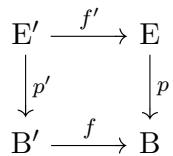
\includegraphics[keepaspectratio]{images/part002_b7191fdb.jpg}}

为笛卡尔方块。假设 E 是 B 的覆叠，且空间 B' 连通并局部道路连通。设 b' 是 B' 的一点，且 \(b = f(b')\)。要使 \((\mathrm{E}', p')\) 成为 B' 的可平凡化覆叠，必要且充分条件是：对于纤维 \(E_b\) 的每一点 x，\(\pi_1(p, x)\) 的像包含 \(\pi_1(f, b)\) 的像。

这由命题 1 以及 I，第 81 页，命题 6 的推论 5 得出。

\subsection{庞加莱群的作用与覆叠的态射}

设 B 是连通且局部道路连通的拓扑空间，b 是 B 的一点。

设 E 是 B 的覆叠。由于假设空间 B 连通，若 E 非空，则纤维 \(E_{b}\) 非空（I，第 74 页，命题 4）。根据 III 第 305 页定理 1 的断言 a)，覆叠 E 连通且非空，当且仅当群 \(\pi_{1}(B,b)\) 在 \(E_{b}\) 上传递作用。

命题 2. --- 设 E 和 E' 是 B 的覆叠。

\begin{enumerate}
\def\labelenumi{\alph{enumi})}
\item
设 \(f\colon\mathrm{E}\to\mathrm{E}^{\prime}\) 是 B-态射。映射 \(f_{b}\colon\mathrm{E}_{b}\to\mathrm{E}_{b}^{\prime}\) 由 \(f\) 导出，分别与 \(\pi_{1}(\mathrm{B},b)\) 在 \(\mathrm{E}_{b}\) 和 \(\mathrm{E}_{b}^{\prime}\) 上的作用相容。当且仅当 \(f\) 是同构时，它是双射。
\item
映射 \(f\mapsto f_{b}\) 是从 B-态射集合 \(\mathcal{C}_{\mathrm{B}}(\mathrm{E};\mathrm{E}^{\prime})\)（其元素是从 E 到 \(\mathrm{E}^{\prime}\) 的 B-态射）到 \(\mathcal{F}_{\pi_1(\mathrm{B},b)}(\mathrm{E}_b;\mathrm{E}_b^{\prime})\)（即 \(\pi_1(\mathrm{B},b)\)-态射集合，其元素是从 \(\mathrm{E}_b\) 到 \(\mathrm{E}_b^{\prime}\) 的态射）的双射。
\end{enumerate}

若 \(f\) 是从 E 到 \(\mathrm{E}'\) 的 B-态射，则映射 \(f_b\colon \mathrm{E}_b\to \mathrm{E}_b'\) 是 \(\pi_1(\mathrm{B},b)\)-态射（参见 III，第 305 页）。此外，两个从 E 到 \(\mathrm{E}'\) 的 B-态射在纤维 \(\mathrm{E}_b\) 上相同，则彼此相等（I，第 80 页，命题 6 的推论 3）。

设 \(\varphi\colon\mathrm{E}_{b}\to\mathrm{E}_{b}^{\prime}\) 是 \(\pi_{1}(\mathrm{B},b)\)-集的态射；证明存在一个 B-态射 \(f\)，它从 E 到 \(\mathrm{E}^{\prime}\) 且满足 \(f_{b}=\varphi\)。不妨设空间 E 和 \(\mathrm{E}^{\prime}\) 连通且非空，于是 \(\mathrm{E}_{b}\) 和 \(\mathrm{E}_{b}^{\prime}\) 是齐性 \(\pi_{1}(\mathrm{B},b)\)-集。设 \(x\) 是 \(\mathrm{E}_{b}\) 的一点；它的稳定子 G 是映射 \(\pi_{1}(p,x)\) 的像（III，第 305 页，定理 1）。由于 \(\varphi\) 是 \(\pi_{1}(\mathrm{B},b)\)-态射，群 G 固定点 \(x^{\prime}=\varphi(x)\)，它属于 \(\mathrm{E}_{b}^{\prime}\)，故 G 包含于映射 \(\pi_{1}(p^{\prime},x^{\prime})\) 的像中。由 III，第 308 页的命题 1，存在一个 B-态射 \(f\)，它从 E 到 \(\mathrm{E}^{\prime}\) 且满足 \(f(x)=x^{\prime}\)。映射 \(f_{b}\) 和 \(\varphi\) 是 \(\pi_{1}(\mathrm{B},b)\)-态射，定义在齐性 \(\pi_{1}(\mathrm{B},b)\)-集 \(\mathrm{E}_{b}\) 到 \(\mathrm{E}_{b}^{\prime}\) 之间，且在点 \(x\) 处相同；所以它们相等。

若 \(f\colon \mathrm{E}\to \mathrm{E}'\) 是 B-同构，则映射 \(f_{b}\colon \mathrm{E}_{b}\to \mathrm{E}_{b}^{\prime}\) 是双射。反之，设映射 \(f_{b}\) 是双射，并令 \(g\colon \mathrm{E}^{\prime}\to \mathrm{E}\) 为满足 \(g_{b} = (f_{b})^{-1}\) 的 B-态射。B-态射 \(g\circ f\colon \mathrm{E}\to \mathrm{E}\) 在 \(\mathrm{E}_b\) 上诱导恒等映射；因此由本命题可知 \(g \circ f = Id_{E}\)。同理，\(f \circ g = Id_{E'}\)，这证明 f 是 B-同构。

推论 1. --- 覆叠 E 和 E' 同构，当且仅当 \(\pi_1(\mathrm{B},b)\)-集 \(\mathrm{E}_b\) 和 \(\mathrm{E}_b'\) 同构。

推论 2. --- 设 (E,p) 和 (E',p') 是 B 的连通覆叠。设 \(x\) 是 \(E_{b}\) 的一点，\(x'\) 是 \(E'_{b}\) 的一点。要存在 B-态射 \(g\colon E\to E'\) 使 \(g(x)=x'\)，必要且充分条件是 \(p_{*}(\pi_{1}(E,x))\subset p'_{*}(\pi_{1}(E',x'))\)。这样的态射唯一；并且当且仅当 \(p_{*}(\pi_{1}(E,x))\) 和 \(p'_{*}(\pi_{1}(E',x'))\) 是 \(\pi_{1}(B,b)\) 的相等子群时，它是同构。

由 III，第 305 页定理 1，从 \(\pi_1(B,b)\) 到 \(E_b\) 的映射由 \(\gamma \mapsto x \cdot \gamma\) 定义，经取商诱导出 \(\pi_1(B,b)\)-集 \(p_*(\pi_1(E,x)) \backslash \pi_1(B,b)\) 到 \(E_b\) 的同构。同样，存在唯一的从 \(\pi_1(B,b)\)-集 \(p'_{*}(\pi_1(E',x')) \backslash \pi_1(B,b)\) 到 \(E_b'\) 的同构。由命题 2，存在一个 B-态射 \(g\colon E\to E'\)，使 \(g(x)=x'\)，当且仅当存在一个 \(\pi_1(B,b)\)-集态射，从 \(p_*(\pi_1(E,x)) \backslash \pi_1(B,b)\) 到 \(p'_{*}(\pi_1(E',x')) \backslash \pi_1(B,b)\)，将类 \(p_*(\pi_1(E,x))\) 送到类 \(p'_{*}(\pi_1(E',x'))\)。这样的态射存在，当且仅当 \(p_*(\pi_1(E,x)) \subset p'_{*}(\pi_1(E',x'))\)。由于假设空间 E 连通，它因而是唯一的（I，第 34 页，命题 11 的推论 2）。当且仅当子群 \(p_*(\pi_1(E,x))\) 和 \(p'_{*}(\pi_1(E',x'))\) 是 \(\pi_1(B,b)\) 的相等子群时，它是同构。

推论 3. --- 设 (E,p) 是 B 的连通覆叠，x 是纤维 \(E_{b}\) 的一点。令 N 表示 \(p_{*}(\pi_{1}(E,x))\) 在 \(\pi_{1}(B,b)\) 中的正规化子。对于 N 的每个元素 \(\gamma\)，存在唯一的 B-自同构 g，使得 \(g(x) = x \cdot \gamma\)；并且映射 \(\gamma \mapsto g\) 经取商定义了从 \(\mathrm{N}/p_{*}(\pi_{1}(\mathrm{E},x))\) 到 \(\mathrm{Aut}_{\mathrm{B}}(\mathrm{E})\) 的群同构。

设 \(\gamma \in \pi_1(\mathrm{B}, b)\)；有 \(p_*(\pi_1(\mathrm{E}, x)) = \operatorname{Int}(\gamma)(p_*(\pi_1(\mathrm{E}, x \cdot \gamma)))\)（III，第 305 页，定理 1，c)）。由推论 2，要存在 B-自同构 \(g\) 使 \(g(x) = x \cdot \gamma\)，必要且充分条件是 \(\gamma\) 属于 N。这样的同构因而唯一。记 \(\alpha: \mathrm{N} \to \mathrm{Aut}_{\mathrm{B}}(\mathrm{E})\) 为由此定义的映射 \(\gamma \mapsto g\)。

设 \(\gamma\) 和 \(\gamma'\) 是 N 的两个元素。置 \(g = \alpha(\gamma)\)、\(g' = \alpha(\gamma')\)；根据关系式 (4)（III，第 305 页）和 (1)（第 304 页），有 \(g(g'(x)) = g(x \cdot \gamma') = g(x) \cdot \gamma' = (x \cdot \gamma) \cdot \gamma' = x \cdot (\gamma\gamma')\)。因此，\(\alpha\) 是群同态。要有 \(\alpha(\gamma) = \mathrm{Id}_{\mathrm{E}}\)，必要且充分条件是 \(x \cdot \gamma = x\)，因为 \(\alpha(\gamma)\) 唯一；也就是说，\(\gamma \in p_*(\pi_1(E, x))\)（III，第 305 页，定理 1，b)）。最后，若 \(g\) 是 E 的 B-自同构，则存在一条道路 \(c\)，它在 E 中连接 \(x\) 与 \(g(x)\)（E 是道路连通的），于是 \(g(x) = x \cdot \gamma\)，其中 \(\gamma\) 是道路 \(p \circ c\) 的类。这证明同态 \(\alpha\) 是满射。

群 \(\mathrm{Aut}_{\mathrm{B}}(\mathrm{E})\) 在纤维 \(\mathrm{E}_b\) 上作用，并被识别为齐性 \(\pi_1(\mathrm{B},b)\)-集 \(\mathrm{E}_b\)（右作用）的自同构群（参见 A，I，第 56 页，命题 5 和 6）。

推论 4. --- 设 (E, p) 是 B 的连通覆叠，x 是纤维 \(E_{b}\) 的一点。要使 E 成为 B 的伽罗瓦覆叠，必要且充分条件是 \(p_{*}(\pi_{1}(E, x))\) 是 \(\pi_{1}(B, b)\) 的正规子群。此时群 \(\mathrm{Aut}_{\mathrm{B}}(\mathrm{E})\) 同构于商群 \(\pi_{1}(\mathrm{B}, b)/p_{*}(\pi_{1}(\mathrm{E}, x))\)。

若 \(p_{*}(\pi_{1}(\mathrm{E},x))\) 是 \(\pi_1(\mathrm{B},b)\) 的正规子群，则根据推论 3，群 \(\mathrm{Aut}_{\mathrm{B}}(\mathrm{E})\) 在纤维 \(\mathrm{E}_b\) 上传递作用，所以 E 是 B 的伽罗瓦覆叠（I，第 102 页，定理 2）。逆命题是 III，第 305 页定理 1 的断言 d)。最后一个断言由推论 3 得出。

\subsection{庞加莱群胚的无局部单值作用}

引理 1. --- 设 B 是局部道路连通的拓扑空间，\(p \colon E \to B\) 和 \(p' \colon E' \to B\) 是满足道路提升性质的平展分离映射（III，第 302 页）。设 \(g \colon E \to E'\) 是满足 \(p' \circ g = p\) 的映射。假设 \(g\) 与群胚 \(\varpi(B)\) 在 \(E\) 和 \(E'\) 上的典范作用相容。则 \(g\) 连续。

设 c 是 E 中的一条道路；置 \(c' = g \circ c\)，并证明映射 \(c'\) 连续。记 B 中的道路 \(p \circ c\) 为 d，并对每个 \(t \in I\)，记 \(d_t\) 为道路 \(s \mapsto d(st)\)。对于所有 \(t \in I\)，有 \(c(t) = c(0) \cdot d_t\)（III，第 304 页，注记 3），由关于 g 的假设，从而有 \(c'(t) = c'(0) \cdot d_t\)，这根据同一注记说明 \(c'\) 是道路 d 的提升。这说明映射 g 按道路连续。由于空间 E 局部道路连通（III，第 261 页，命题 2 的推论 2），映射 g 连续（III，第 269 页，命题 13 的推论）。

设 B 是拓扑空间。考虑一种作用 \(\varphi = (\varphi_{a,b})_{(a,b)\in \mathrm{B}\times \mathrm{B}}\)，它是群胚 \(\varpi (\mathrm{B})\) 关于映射 \(p\colon \mathrm{E}\to \mathrm{B}\) 在集合 E 上的作用。称 \(\varpi (\mathrm{B})\) 在 E 上无单值性地作用，若对每个 \(b\in \mathrm{B}\) 和每个圈类 \(\gamma \in \pi_1(\mathrm{B},b)\)，\(\gamma\) 在纤维 \(\mathrm{E}_b\) 上的作用是平凡的，则称作用 \(\varphi\)（即群胚 \(\varpi (\mathrm{B})\) 的作用）无单值性地作用在 E 上（参见 II，第 168 页）。若 B 道路连通，只需对 B 的一个点验证这一点即可（同上）。如果 B 的每一点都有邻域 V，使得 \(\varpi (\mathrm{V})\) 在集合 \(\mathrm{E_V} = p^{-1}(\mathrm{V})\) 上关于映射 \(p_{\mathrm{V}} = p\mid p^{-1}(\mathrm{V})\) 无单值性地作用，则称群胚的作用无局部单值性。

注记。--- 设 B 是局部道路连通的拓扑空间，并假设 B 的每一点 b 都有邻域 V，使得 \(\pi_{1}(V,b)\) 在 \(\pi_{1}(B,b)\) 中的像约化为单位元（参见 IV，第 340 页，定义 2）。那么，群胚 \(\varpi(B)\) 的每个作用都无局部单值性。

事实上，考虑集合 E、映射 \(p \colon \mathrm{E} \to \mathrm{B}\) 以及作用 \(\varphi\)；它是群胚 \(\varpi(\mathrm{B})\) 关于 \(p\) 在 E 上的作用。设 \(a\) 是 B 的一点，V 是 \(a\) 的邻域，并且 \(\pi_1(\mathrm{V}, a)\) 在 \(\pi_1(\mathrm{B}, a)\) 中的像约化为单位元。设 U 是包含于 V 的 \(a\) 的道路连通邻域。设 \(b\) 是 U 的一点，\(\gamma \in \pi_1(\mathrm{U}, b)\)。设 \(\delta\) 是 U 中连接 \(a\) 与 \(b\) 的道路的类。于是，\(\delta\gamma\delta^{-1}\) 是 U 中以 \(a\) 为基点的圈的类；因此，它在 \(\pi_1(\mathrm{B}, a)\) 中的像是平凡的。从而有 \(\varphi_{a,a}(\delta\gamma\delta^{-1}) = \mathrm{Id}_{\mathrm{E}_a}\)，所以 \(\varphi_{b,b}(\gamma) = \mathrm{Id}_{\mathrm{E}_b}\)。这说明 \(\varpi(\mathrm{U})\) 关于 U-空间 \(\mathrm{E_U}\) 的作用无单值性。因此，作用 \(\varphi\) 无局部单值性。

命题 3. --- 设 B 是局部道路连通的拓扑空间，E 是赋有作用 \(\varphi\)（群胚 \(\varpi(B)\) 的作用）的集合，该作用关于映射 \(p: E \to B\) 无局部单值性。于是 E 上存在唯一的拓扑，使得下列条件成立：

\begin{enumerate}
\def\labelenumi{(\roman{enumi})}
\item
  赋予此拓扑的集合 E 连同映射 p 是 B 的覆叠；
\item
  \(\varpi(\mathrm{B})\) 在此覆叠上的典范作用与作用 \(\varphi\) 相同。
\end{enumerate}

这种拓扑的唯一性由 III，第 312 页的引理 1 得出，其中取 E 的恒等映射作为 g。为证明其存在性，还可假设 B 连通且非空。

首先假设作用 \(\varphi = (\varphi_{a,b})_{(a,b)\in \mathrm{B}\times \mathrm{B}}\) 是群胚 \(\varpi (\mathrm{B})\) 关于 \(p\) 在集合 E 上的无单值作用。

设 \(a\) 是 B 的一点。对于每个 \(b \in \mathrm{B}\)，存在一条道路 \(c\) 在 B 中连接点 \(a\) 与点 \(b\)。若 \(\gamma \in \varpi_{a,b}(\mathrm{B})\) 表示道路 \(c\) 的类，则双射 \(\varphi_{a,b}(\gamma) \colon \mathrm{E}_a \to \mathrm{E}_b\) 与道路 \(c\) 无关，因为该作用无单值性；将此双射记为 \(f_{a,b}\)。映射 \(\Phi_a \colon \mathrm{B} \times \mathrm{E}_a \to \mathrm{E}\)（由 \((b,x) \mapsto f_{a,b}(x)\) 定义）是双射；其逆双射将 \(x \in \mathrm{E}\) 映到二元组 \((p(x), f_{p(x),a}(x))\)。赋予集合 \(\mathrm{E}_a\) 离散拓扑，于是 B-空间 \(\mathrm{B} \times \mathrm{E}_a\) 是 B 的平凡覆叠。通过结构转移，双射 \(\Phi_a\) 在 E 上赋予一个拓扑，使其成为 B 的覆叠。

证明 \(\varpi(\mathrm{B})\) 在 E 上的典范作用与作用 \(\varphi\) 相同。设 \(x\) 是 \(\mathrm{E}_a\) 的一点，设 \(b\) 是 B 的一点。设 \(c\) 是 B 中连接点 \(a\) 与点 \(b\) 的道路；映射 \(t \mapsto \Phi_a(c(t), x)\) 是 E 中连接点 \(x\) 与点 \(\Phi_a(b, x) = f_{a,b}(x)\) 的道路。若 \(\gamma \in \varpi_{a,b}(\mathrm{B})\) 表示道路 \(c\) 的类，则有 \(x \cdot \gamma = f_{a,b}(x)\)。这说明 \(\varpi(\mathrm{B})\) 在覆叠 E 上的典范作用与作用 \(\varphi\) 在起点为 \(a\) 的道路类上相同。由于这些类生成群胚 \(\varpi(\mathrm{B})\)，两个作用相同。

现在处理一般情形。令 \(\mathcal{B}\) 为 E 的开子集 V 的集合，其中 \(\varpi(\mathrm{V})\) 在 \(p^{-1}(\mathrm{V})\) 上无单值性地作用。根据假设，\(\mathcal{B}\) 中的元素覆盖 B。由上文，对于每个 \(\mathrm{V} \in \mathcal{B}\)，在集合 \(p^{-1}(\mathrm{V})\) 上存在唯一拓扑，使得 \((p^{-1}(\mathrm{V}), p_{\mathrm{V}})\) 成为 V 的覆叠，并且 \(\varpi(\mathrm{V})\) 在此覆叠上的典范作用与 \(\varphi\) 诱导的作用相同。

设 \(V' \in \mathcal{B}\)。上面定义的在 \(p^{-1}(V \cap V')\) 上由 \(p^{-1}(V)\) 的拓扑（分别由 \(p^{-1}(V')\) 的拓扑）诱导的拓扑，确实使其成为 \(V \cap V'\) 的覆叠，并且 \(\varpi(V \cap V')\) 在其上的典范作用由作用 \(\varphi\) 诱导。因此这些拓扑都与 \(p^{-1}(V \cap V')\) 的拓扑相同。于是存在 E 上唯一的拓扑，在每个 \(p^{-1}(V)\) 上诱导出先前定义的拓扑（参见 I，§2，第 16 页）。

赋予 E 此拓扑后，映射 p 连续，且 B-空间 E 是覆叠。\(\varpi(\mathrm{B})\) 的典范作用与作用 \(\varphi\) 在像包含于 \(\mathcal{B}\) 中某个开集内的道路类上相同。由引理 4 的

III，第 272 页，这些类生成群胚 \(\varpi(B)\)。因此这两个作用相同（II，第 167 页）。

推论。--- 设 B 是连通且局部道路连通的拓扑空间，(E,p) 是 B-空间，其投影 p 是平展、分离且具有道路提升性质的映射。若 \(\varpi(\mathrm{B})\) 关于 p 在集合 E 上的典范作用无局部单值性，则 E 是 B 的覆叠。

给 E 赋予由道路提升定义的 \(\varpi(B)\) 的典范作用（III，第 303 页，编号 3）。E 上存在一个拓扑，使条件 (i) 和 (ii) 的命题 3 得以满足。根据 III，第 312 页的引理 1，此拓扑与 E 上给定的拓扑相同。

\subsection{庞加莱群的容许拓扑}

设 B 是拓扑空间，\(a\) 是 B 的一点。称 \(\pi_1(B, a)\) 的子群 H 为容许的，如果 B 的每一点 \(b\) 都有邻域 V，使得 \(\gamma i_*(\delta)\gamma^{-1} \in \mathrm{H}\) 对每个 \(\gamma \in \varpi_{a,b}(\mathrm{B})\) 和每个 \(\delta \in \pi_1(V, b)\) 都成立，其中 \(i: V \to B\) 是典范嵌入。如果 H 是 \(\pi_1(B, a)\) 的正规子群，则要使 H 容许，只需对一个道路类 \(\gamma \in \varpi_{a,b}(\mathrm{B})\) 验证此条件即可。

命题 4. — \(\pi_1(B, a)\) 上存在唯一一个与其群结构相容的拓扑，使 \(\pi_1(B, a)\) 的容许正规子群构成单位元的邻域基。在此拓扑下，开子群恰好是容许子群。

由容许子群的定义得到以下事实：

\begin{enumerate}
\def\labelenumi{\alph{enumi})}
\item
  群 \(\pi_1(B, a)\) 是容许的；
\item
  包含某个容许子群的子群是容许的；
\item
  有限个容许子群的交是容许的。
\item
对于 \(\pi_{1}(B,a)\) 的每个容许子群 H，各子群 \(\gamma H\gamma^{-1}\) 的交（其中 \(\gamma\) 遍历 \(\pi_{1}(B,a)\)）是容许的。
\end{enumerate}

特别地，容许正规子群的集合是一个滤基，由 \(\pi_1(B,a)\) 中满足公理 (GV \(_{\text{III}}'\) ) 的子群组成；根据 TG，III，第 5 页，例，这就得到命题的第一部分。第二部分随即显然（参见 TG，III，第 7 页，命题 4 的推论）。

命题 4 所刻画的群 \(\pi_{1}(B,a)\) 上的拓扑称为容许拓扑。

注记。--- 1) 若 B \(_{0}\) 表示 B 中 \(a\) 的道路连通分支，则在这些群赋予容许拓扑时，典范同构 \(\pi_{1}(B_{0}, a) \to \pi_{1}(B, a)\) 是拓扑群同构。

\begin{enumerate}
\def\labelenumi{\arabic{enumi})}
\setcounter{enumi}{1}
\item
设 B 是拓扑空间。设 \(b\) 和 \(b'\) 是属于同一道路连通分支的 B 的点，并设 \(\gamma\) 是 \(\varpi_{b,b'}(B)\) 的元素。由容许子群的定义，对于 \(\pi_1(B,b')\) 的每个容许子群 H，子群 \(\gamma H\gamma^{-1}\) 是 \(\pi_1(B,b)\) 的容许子群。因此，同构 \(u_\gamma \colon \delta \mapsto \gamma \delta \gamma^{-1}\) 从 \(\pi_1(B,b')\) 到 \(\pi_1(B,b)\)（参见 III，第 292 页）在这些群赋予容许拓扑时是同胚。
\item
  设 A 和 B 是拓扑空间，\(a\) 是 A 的一点，\(f\colon\mathrm{A}\to\mathrm{B}\) 是连续映射。置 \(b=f(a)\)。若 H 是 \(\pi_{1}(\mathrm{B},b)\) 的容许子群，则它在同态 \(\pi_{1}(f,a)\) 下的逆像是 \(\pi_{1}(\mathrm{A},a)\) 的容许子群。因此，当这些群赋予容许拓扑时，群同态 \(\pi_{1}(f,a)\colon\pi_{1}(\mathrm{A},a)\to\pi_{1}(\mathrm{B},b)\) 连续。
\end{enumerate}

命题 5. --- 设 B 是局部道路连通的拓扑空间，a 是 B 的一点。要使 \(\pi_1(\mathrm{B},a)\) 的子群 H 容许，必要且充分条件是存在 B 的覆叠 (E,p) 以及一点 \(x\in \mathrm{E}_a\)，使得 \(\mathrm{H} = p_{*}(\pi_{1}(\mathrm{E},x))\)。

设 \((\mathrm{E},p)\) 是 B 的覆叠，设 x 是 \(E_{a}\) 的一点；置 \(\mathrm{H}=p_{*}(\pi_{1}(\mathrm{E},x))\)，并证明它是 \(\pi_{1}(\mathrm{B},a)\) 的容许子群。设 b 是 B 的一点，V 是 b 的邻域，并且 \(\mathrm{E}_{\mathrm{V}}=(p^{-1}(\mathrm{V}),p_{\mathrm{V}})\) 是 V 的可平凡化覆叠。设 \(\gamma\in\varpi_{a,b}(\mathrm{B})\)；证明对于每个 \(\delta\in\pi_{1}(\mathrm{V},b)\)，道路类 \(\gamma\delta\gamma^{-1}\) 属于 H。

由 III，第 301 页命题 3，存在唯一的道路严格同伦类 \(\gamma'\)，其起点为 E 中的 \(x\)，且 \(p_*(\gamma') = \gamma\)。设 \(y\) 是 \(\gamma'\) 的终点；有 \(p(y) = b\)（III，第 302 页，命题 4）。再令 \(\delta'\) 为 E 中起点为 \(y\) 且满足 \(p_*(\delta') = \delta\) 的唯一道路类。由于 \(\mathrm{E_V}\) 可平凡化，\(\delta'\) 是以 \(y\) 为基点的圈的类。于是，\(\gamma'\delta'(\gamma')^{-1}\) 是 E 中以 \(a\) 为基点的圈的类，其在 \(p_*\) 下的像是类 \(\gamma\delta\gamma^{-1}\)，这正是要证明的。

反之，设 H 是 \(\pi_1(B, a)\) 的容许子群。令 \(\lambda_a(B)\) 为对道路严格同伦关系取商所得的空间 \(\Lambda_a(B)\) 的商集，其中道路的起点为 \(a\)；由于严格同伦的道路具有相同的终点，终点映射 \(e: \Lambda_a(B) \to B\) 经取商定义了映射 \(\varepsilon: \lambda_a(B) \to B\)。道路类的复合赋予集合 \(\lambda_a(B)\) 以群 \(\pi_1(B, a)\) 的左作用。将此作用限制为群 H 的作用，并将其轨道集合记为 \(H\backslash\lambda_a(B)\)。

映射 \(\varepsilon\colon\lambda_{a}(B)\to B\) 经取商诱导出映射 \(q\colon H\backslash\lambda_{a}(B)\to B\)。道路类的复合赋予集合 \(H\backslash\lambda_a(B)\) 以群胚 \(\varpi(B)\) 关于映射 \(q\) 的右作用。

此作用无局部单值性。事实上，设 \(b\) 是 B 的一点，V 是 \(b\) 的一个邻域，使得 \(\gamma i_{*}(\pi_{1}(V,b))\gamma^{-1}\subset H\) 对每个道路类 \(\gamma\) 都成立，其中这些道路连接 B 中的 \(a\) 与 \(b\)，而 \(i\) 表示 V 到 B 的嵌入。由于 B 局部道路连通，还可进一步假设 V 道路连通。设 \(c\in V\)，令 \(\delta\) 为 \(\pi_1(B,c)\) 中的、以 \(c\) 为基点且像包含于 V 的圈的类，并令 \(\delta'\) 为 \(\lambda_a(B)\) 中满足 \(\varepsilon (\delta ') = c\) 的元素。令 \(\delta''\) 为 \(\varpi_{c,b}(V)\) 的元素，并置 \(\gamma = \delta '\delta ''\)。根据 V 的定义，\(\delta '\delta (\delta ')^{-1} = \gamma ((\delta '')^{-1}\delta \delta '')\gamma^{-1}\) 是 \(\pi_1(B,a)\) 中的元素，并属于 H。于是，\(\mathrm{H}\delta^{\prime}\cdot \delta = \mathrm{H}\delta^{\prime}\)；这证明 \(\pi_1(V,c)\) 在集合 \(q^{-1}(c)\) 上的作用是平凡的。

由 III，第 313 页命题 3，\(\mathrm{H}\backslash\lambda_{a}(\mathrm{B})\) 上存在唯一拓扑，使得 \(q\) 连续，B-空间 \((\mathrm{H}\backslash\lambda_{a}(\mathrm{B}),q)\) 是覆叠，并且 \(\varpi(\mathrm{B})\) 在此覆叠上的典范作用就是上面定义的作用。根据 III 第 305 页定理 1 的断言 b)，群 \(q_{*}(\pi_{1}(\mathrm{H}\backslash\lambda_{a}(\mathrm{B}),\mathrm{H}))\) 等于 H。

称群 \(\pi_1(B, b)\) 在集合 X 上的作用为容许的，如果典范映射 \(\pi_1(B, b) \to \mathfrak{S}_{\mathrm{X}}\) 的核是 \(\pi_1(B, b)\) 的开子群。这等价于说，同态 \(\pi_1(B, b) \to \mathfrak{S}_{\mathrm{X}}\) 在群 \(\mathfrak{S}_{\mathrm{X}}\) 赋予离散拓扑时是连续的。于是，当 X 赋予离散拓扑时，映射 \(\pi_1(B, b) \times X \to X\) 连续。反之，考虑 \(\pi_{1}(B,b)\) 在离散空间 X 上的连续作用。设 x 是 X 的一点；根据假设，它的稳定子是 \(\pi_{1}(B,b)\) 的开子群 H。对于 \(\gamma\in\pi_{1}(B,b)\)，\(\gamma\cdot x\) 的固定子是子群 \(\gamma H\gamma^{-1}\)，因此 \(\pi_{1}(B,b)\) 中固定 x 的轨道的每个元素的子群，是各子群 \(\gamma H\gamma^{-1}\) 的交（其中 \(\gamma\) 遍历 \(\pi_{1}(B,b)\)）。它是开子群，因为 \(\pi_{1}(B,b)\) 的正规开子群构成其拓扑的基（III，第 315 页，命题 4）。这说明，\(\pi_{1}(B,b)\) 在离散空间 X 上的连续作用，只要是传递的，或者更一般地说，只要 X 中各元素的轨道集合是有限的，就是容许的。

对于任意离散群 \(G\)、任意以 \(G\) 为群的主覆叠 \(E\) 在 \(B\) 上，以及任意点 \(x \in E_{b}\)，回顾映射 \(h_{(\mathrm{E},x)}\) 从 \(\pi_{1}(\mathrm{B},b)\) 到 G，它把 \(\gamma \in \pi_{1}(\mathrm{B},b)\) 关联到 G 中的唯一元素 \(g \in G\)，该元素满足 \(x \cdot g = x \cdot \gamma^{-1}\)，是群同态（III，第 306 页，命题 5）。

命题 6. --- 设 B 是拓扑空间，b 是 B 的一点。给群 \(\pi_1(B, b)\) 赋予容许拓扑。

\begin{enumerate}
\def\labelenumi{\alph{enumi})}
\item
  对于任意离散群 G、以 G 为群的 B 的主覆叠 E 以及任意 \(x \in E_{b}\)，同态 \(h_{(E,x)}\) 是拓扑群的连续同态。
\item
  对于 B 的每个覆叠 E，\(\pi_{1}(B,b)\) 在纤维 \(E_{b}\) 上的典范作用都是容许的。
\end{enumerate}

只需证明第二个断言。令 K 为满足 \(k \in \pi_{1}(B, b)\) 且 \(x \cdot k = x\) 对所有 \(x \in E_{b}\) 都成立的元素 k 所成的集合。证明 K 是 \(\pi_{1}(B, b)\) 的容许子群。

设 \(b'\) 是 B 的一点，\(V'\) 是 B 中 \(b'\) 的邻域，在其上方覆叠 E 可平凡化。设 \(\gamma\) 是 B 中连接 \(b\) 与 \(b'\) 的道路 c 的类，\(c'\) 是 E 中从 x 出发且提升 c 的唯一道路。对于所有 \(\delta \in \pi_1(V', b')\) 和每个 \(x' \in E_{b'}\)，有 \(x' \cdot \delta = x'\)。因此，对于 \(x \in E_b\) 和 \(\delta \in \pi_1(V', b')\)，有

\[
x \cdot \gamma \delta \gamma^ {- 1} = ((x \cdot \gamma) \cdot \delta) \cdot \gamma^ {- 1} = (x \cdot \gamma) \cdot \gamma^ {- 1} = x,
\]

所以 \(\gamma\delta\gamma^{-1}\) 属于 K。换言之，K 是容许子群，命题得证。

命题 7. --- 设 B 是连通且局部道路连通的拓扑空间，b 是 B 的一点。给群 \(\pi_1(B, b)\) 赋予容许拓扑。

\begin{enumerate}
\def\labelenumi{\alph{enumi})}
\item
  设 G 是离散拓扑群。对于每个连续同态 \(f\colon \pi_{1}(\mathrm{B},b)\to \mathrm{G}\)，存在以 G 为群的 B 的主覆叠 E 以及一点 \(x\) 属于 \(\mathrm{E}_{b}\)，使得 \(h_{(\mathrm{E},x)} = f\)。
\item
  对于每个赋有群 \(\pi_{1}(B,b)\) 的容许右作用的离散拓扑空间 F，存在 B 的覆叠 E，使得 \(\pi_{1}(B,b)\)-集 F 和 \(E_{b}\) 同构。
\end{enumerate}

证明 \(a\)。设 \(f\) 是从 \(\pi_1(B, b)\) 到离散群 G 的连续同态。其核是 \(\pi_1(B, b)\) 的开正规子群 K；令 H 为群 \(\pi_1(B, b)/K\)，令 \(\overline{f} \colon H \to G\) 为 \(f\) 经取商诱导的群同态。由 III，第 316 页命题 5，存在 B 的连通覆叠 E'，使得子群 K 是纤维 \(E'_{b}\) 的每一点的稳定子；覆叠 E' 是以 H = \(\pi_1(B, b)/K\) 为群的主覆叠。设 \(x'\) 是 \(E'_{b}\) 的一点；同态 \(h_{(E', x')} \colon \pi_1(B, b) \to H\) 是满射且核为 K（III，第 306 页，命题 5）。再令 \(\varphi \colon H \to G\) 为唯一的群同态，使得 \(\varphi \circ h_{(E', x')} = f\)。B 的相伴覆叠 \(E = E' \times^{H} G\) 是以 G 为群的主覆叠，并且有 \(h_{(E, x)} = \varphi \circ h_{(E', x')} = f\)（III，第 307 页，例 2）。断言 \(a\) 得证。

证明 \(b\)。设 F 是赋有群 \(\pi_1(B,b)\) 的容许右作用的集合。记 \(f: \pi_1(B,b) \to \mathfrak{S}_{\mathrm{F}}\) 为此作用，并给群 \(\mathfrak{S}_{\mathrm{F}}\) 赋予离散拓扑。由 \(a\)，存在以 \(\mathfrak{S}_{\mathrm{F}}\) 为群的 B 的主覆叠 E 以及一点 \(x \in \mathrm{E}\)，使得同态 \(h_{(\mathrm{E},x)}\) 等于 \(f\)。群 \(\pi_1(B,b)\) 在点 \(b\) 上的相伴覆叠 \(\mathrm{E} \times^{\mathfrak{S}_{\mathrm{F}}} \mathrm{F}\) 的纤维，被识别为 \(\pi_1(B,b)\) 在 F 上的作用（III，第 306 页，例 1）。

注记。--- 4) \(\pi_1(B, b)\) 上的容许拓扑是使 \(\pi_1(B, b)\) 在每个 B 的连通覆叠 E 的 \(E_b\) 上的作用连续的最粗拓扑（III，第 318 页，命题 6 和第 318 页，命题 7）。若 E 是 B 的连通覆叠，且 \(x\) 是纤维 \(E_b\) 的一点，则映射 \(c' \mapsto c'(1)\) 从 \(\Lambda_x(E)\) 到 E 连续。因此，映射 \(c \mapsto x \cdot c\) 从 \(\Lambda_b(B)\) 到 E 连续（III，第 302 页，命题 3 的推论 2）。通过限制到 \(\Omega_b(B)\) 并取商，得到映射 \(\gamma \mapsto x \cdot \gamma\)，当给群 \(\pi_1(B, b)\) 赋予 \(\Omega_b(B)\) 的商拓扑时该映射连续。因此，\(\pi_{1}(B,b)\) 上的容许拓扑比紧收敛拓扑的商拓扑更粗。它可以严格更粗（III，第 337 页，习题 7）。

\begin{enumerate}
\def\labelenumi{\arabic{enumi})}
\setcounter{enumi}{4}
\tightlist
\item
设 B 是连通且局部道路连通的拓扑空间，\(a\) 是 B 的一点，H 是 \(\pi_1(B,a)\) 的子群。由上面的注记，若 H 容许，则它对于紧收敛拓扑的商拓扑也是开子群。反之，设 H 是 \(\pi_1(B,a)\) 的正规子群，且对于紧收敛拓扑的商拓扑为开子群。设 \(x\) 是 B 的一点，\(\gamma \in \varpi_{a,x}(B)\)。此时 \(\gamma^{-1}H\gamma\) 是 \(\pi_1(B,x)\) 的子群，对紧收敛拓扑的商拓扑仍是开子群（III，第 293 页，注记 3）。于是存在 B 中 \(x\) 的邻域 V，使得 \(\gamma^{-1}H\gamma\) 包含每个像包含于 V 的、以 \(x\) 为基点的圈的类。因此有 \(\gamma \pi_1(V,x)\gamma^{-1} \subset H\)；由于 H 正规，这说明 H 是 \(\pi_1(B,a)\) 的容许子群。
\end{enumerate}

\exerciseshdr{习题}

\exercisegroup

\begin{enumerate}
\def\labelenumi{\arabic{enumi})}
\tightlist
\item
  对于每个 \(\theta \in \mathbf{R}\)，令 \(C_{\theta}\) 为平面中端点为 \((0,0)\) 和 \((\cos(2\pi\theta), \sin(2\pi\theta))\) 的线段；置
\end{enumerate}

\[
\mathrm{C} = \bigcup_ {\theta \in \mathbf {Q} \cap [ 1 / 6, 1 / 4 ]} \mathrm{C} _ {\theta}.
\]

\begin{enumerate}
\def\labelenumi{\alph{enumi})}
\item
  空间 C 在 0 处可缩，但在任何其他点处都不可缩。
\item
  令 D 为 C 的平移 \((0, n) + \mathrm{C}\)（\(n \in Z\)）之并。证明空间 D 同伦等价于一点，但在其任何一点处都不可缩。
\end{enumerate}

\begin{enumerate}
\def\labelenumi{\arabic{enumi})}
\setcounter{enumi}{1}
\tightlist
\item
  设 B 是 \(\mathbf{R}^{n}\) 的子集，\(a\) 是 B 内部的一点；记 S 为 B 的边界。假设 B 关于 \(a\) 是星形的，且每条起点为 \(a\) 的半直线都与 S 交于唯一一点。令 \(f\colon\mathbf{R}_{+}^{*}\times\mathrm{S}\to\mathbf{R}^{n}-\{a\}\) 为由 \(f(t,y)=ty+(1-t)a\) 定义的映射。证明 \(f\) 是同胚，并且满足 \(f([0,1]\times\mathrm{S})=\mathrm{B}-\{a\}\) 和 \(f(\{1\}\times\mathrm{S})=\mathrm{S}\)。
\end{enumerate}

当 B 是 \(R^{n}\) 的凸、闭且有界子集，a 是 B 的附着点时，该结果尤其适用（参见 I，第 123 页，命题 2 以及 EVT，II，第 15 页，命题 16）。

\begin{enumerate}
\def\labelenumi{\arabic{enumi})}
\setcounter{enumi}{2}
\item
  设 X 是将空间 R 中的子集 Q 缩塌所得的拓扑空间（III，第 252 页，定义 10）。典范满射 \(p: R \rightarrow X\) 既非开映射也非闭映射。
\item
  设 X 是 R 中的区间 \([-1,1]\)，令 A = X - \{0\}。X 到 X/A 的典范映射是同伦等价，但不存在起点为 \(\mathrm{Id}_{X}\) 且满足 III 第 252 页命题 10 的假设的同伦 σ。
\item
  令 A 为 \(\mathbf{R}\) 中形如 \(1/n\) 的实数集合的闭包，其中 \(n\) 遍历满足 \(\geqslant 1\) 的整数集合。令 \(i\) 为 A 到 \(\mathbf{R}\) 的典范嵌入。由 \(\mathrm{Côn}(i)\) 到 \(\mathbf{R}/\mathrm{A}\) 的典范映射不是同伦等价。
\item
  设 X 是可度量化的可数型拓扑空间。称 X 为绝对收缩核\(^{(1)}\)，如果对于每个可度量化的可数型拓扑空间 Y、Y 的每个闭子集 B 以及每个连续映射 \(f: B \to X\)，映射 f 都能延拓为从 Y 到 X 的连续映射。
\end{enumerate}

\begin{enumerate}
\def\labelenumi{\alph{enumi})}
\item
  设 X 是可度量化的可数型拓扑空间。要使 X 成为绝对收缩核，必要且充分条件是：对于每个可度量化的可数型空间 Y 以及每个从 X 到 Y 的连续、单射且闭映射 f，都存在连续映射 \(g: Y \to X\)，使得 \(g \circ f = Id_{X}\)。
\item
  证明空间 I 和 R 是绝对收缩核。
\item
  证明绝对收缩核的可数族的乘积空间是绝对收缩核。
\item
  设 X 是绝对收缩核，A 是 X 的子空间且是 X 的收缩核。证明 A 是绝对收缩核。
\end{enumerate}

\begin{enumerate}
\def\labelenumi{\arabic{enumi})}
\setcounter{enumi}{6}
\tightlist
\item
  设 X 是可度量化的可数型拓扑空间。如果对于每个可度量化的可数型拓扑空间 Y、Y 的每个闭子集 B 以及每个连续映射 \(f: B \rightarrow X\)，映射 f 都能延拓为从 B 的某个邻域到 X 的连续映射，则称 X 为绝对邻域收缩核。
\end{enumerate}

\begin{enumerate}
\def\labelenumi{\alph{enumi})}
\item
  设 X 是可度量化的可数型拓扑空间。要使 X 成为绝对邻域收缩核，必要且充分条件是：对于每个可度量化的可数型空间 Y 以及每个从 X 到 Y 的连续、单射且闭映射 f，都存在 \(f(\mathrm{X})\) 的一个邻域 U 以及连续映射 \(g: U \to X\)，使得 \(g \circ f = Id_{X}\)。
\item
  设 X 是绝对邻域收缩核，A 是 X 的子集。若 A 有一个邻域 U，且 A 是 U 的收缩核，则 A 是绝对邻域收缩核。特别地，X 的每个开子集以及 X 的每个收缩核都是绝对邻域收缩核。
\item
  证明绝对邻域收缩核的有限族的乘积空间是绝对邻域收缩核。
\end{enumerate}

d) 证明球面 \(\mathbf{S}_n\) 是绝对邻域收缩核。

\begin{enumerate}
\def\labelenumi{\alph{enumi})}
\setcounter{enumi}{4}
\item
  设 X 是可度量化的可数型拓扑空间，\(A_{1}\) 和 \(A_{2}\) 是 X 的闭子集，且 \(X = A_{1} \cup A_{2}\)。假设 \(A_{1} \cap A_{2}\) 是绝对邻域收缩核。要使 X 成为绝对邻域收缩核，必要且充分条件是 \(A_{1}\) 和 \(A_{2}\) 也具有同样性质。
\item
  设 X 是可度量化的可数型拓扑空间。若 X 是两个绝对邻域收缩核开子集之并，则 X 是绝对邻域收缩核。
\item
  设 X 是可度量化的可数型拓扑空间，且每一点都有一个绝对邻域收缩核的邻域。证明 X 是绝对邻域收缩核。
\end{enumerate}

\begin{enumerate}
\def\labelenumi{\arabic{enumi})}
\setcounter{enumi}{7}
\tightlist
\item
  设 X 是可度量化的拓扑空间；设 d 是定义其拓扑的度量。令 \(\mathcal{C}_{b}(\mathrm{X};\mathbf{R})\) 为 X 上连续且有界的实值函数构成的向量空间；给它赋予由 \(\|f\| = \sup_{x \in X} |f(x)|\)（\(f \in \mathcal{C}_{b}(\mathrm{X};\mathbf{R})\)）定义的范数。
\end{enumerate}

\begin{enumerate}
\def\labelenumi{\alph{enumi})}
\item
  定义映射 \(j\colon X \to \mathcal{C}_{b}(X; \mathbf{R})\)，其定义为 \(j(x)\colon y \mapsto d(x, y)/(1 + d(x, y))\)。证明映射 j 诱导从 X 到其像的同胚。
\item
  令 V 为 \(\mathcal{C}_{b}(\mathrm{X};\mathbf{R})\) 中所有包含 \(j(\mathrm{X})\) 的凸子集之交。证明 \(j(\mathrm{X})\) 在 V 中是闭的。
\item
  设 X 是可度量化的可数型空间。证明存在 \(I^{N}\) 的凸子集 Z，使得 X 同胚于 Z 的一个闭子集。
\end{enumerate}

\begin{enumerate}
\def\labelenumi{\arabic{enumi})}
\setcounter{enumi}{8}
\tightlist
\item
  如果 X、Y 是拓扑空间，U 是 X 的子集族，则称映射 \(f, g: Y \to X\) 为 U-邻近的，如果对于每个 \(y \in Y\)，存在 \(U \in U\)，使得 \(f(y)\) 和 \(g(y)\) 都属于 U；称同伦 \(\sigma: Y \times I \to X\) 为 U-小的，如果对于每个 \(y \in Y\)，存在 \(U \in U\)，使得 \(\sigma(y, t) \in U\) 对所有 \(t \in I\) 都成立。
\end{enumerate}

设 X 是 \(I^{N}\) 的凸子集 Z 的闭子空间（参见习题 8）；假设 X 是绝对邻域收缩核。

\begin{enumerate}
\def\labelenumi{\alph{enumi})}
\item
  设 U 是由 \(I^{N}\) 的开子集构成的 X 的覆盖。证明存在 \(I^{N}\) 的开凸子集族 V，使得对于每个开集 \(v \in V\)，存在开集 \(u \in U\)，满足 \(v \cap X \subset u\)，并且存在 X 到族 V 的并集中的典范嵌入的连续收缩映射 r。
\item
  设 Y 是拓扑空间，B 是 Y 的闭子空间。设 \(f, g: \mathrm{Y} \to \mathrm{X}\) 是 \(\mathcal{V}\)-邻近的连续映射，\(\sigma: \mathrm{B} \times \mathbf{I} \to \mathrm{X}\) 是 \(\mathcal{V}\)-小的同伦，且其起点等于 \(f|_{\mathrm{B}}\)。
\end{enumerate}

  证明存在 Y 中 B 的一个邻域 W，以及从子空间 \((\mathbf{Y} \times \{0,1\}) \cup (\mathbf{W} \times \mathbf{I})\)（它是 \(Y \times I\) 的子空间）到 X 的连续映射 h，使得 \(h(y,0) = f(y)\) 和 \(h(y,1) = g(y)\) 对所有 \(y \in Y\) 都成立，并且 \(h(y,t) = \sigma(y,t)\) 对所有 \(y \in B\) 和每个 \(t \in I\) 都成立。证明存在包含于 W 的 B 的一个邻域 \(W'\)，使得 \(h \mid W' \times I\) 是 \(\mathcal{V}\)-小同伦。

\begin{enumerate}
\def\labelenumi{\alph{enumi})}
\setcounter{enumi}{2}
\tightlist
\item
  设 \(u \colon \mathrm{Y} \to \mathbf{I}\) 是连续映射，满足 \(u(y) = 1\) 对 \(y \in \mathrm{B}\) 成立，且 \(u(y) = 0\) 在 \(\mathrm{Y} - \mathrm{W}\) 的某个邻域上成立；置
\end{enumerate}

\[
h ^ {\prime} (y, t) = \left\{ \begin{array}{l l} (1 - u (y)) ((1 - t) f (y) + t g (y)) + u (y) h (y, t) & \text { if } y \in \mathrm{V} \\ (1 - t) f (y) + t g (y) & \text { otherwise. } \end{array} \right.
\]

证明 \(h'\) 连续且其像包含于 V。

\(d)\) 推出存在同伦 \(\widetilde{\sigma}\colon\mathbf{Y}\times\mathbf{I}\to\mathbf{X}\)，其起点为 \(f\)、终点为 \(g\)，且是 \(\mathcal{U}\)-小的。

\begin{enumerate}
\def\labelenumi{\arabic{enumi})}
\setcounter{enumi}{9}
\tightlist
\item
  设 X 是拓扑空间。假设 X 有一个开覆盖 U，使得对于每个拓扑空间 Y 和 Y 的每个闭子空间 B，从 Y 到 X 的两个 U-邻近映射 \(f_{0}, f_{1}\)，只要存在连接 \(f_{0} \mid B\) 与 \(f_{1} \mid B\) 的 U-小同伦，它们就是同伦的。
\end{enumerate}

\begin{enumerate}
\def\labelenumi{\alph{enumi})}
\item
  设 a 是 X 的一点，U 是 U 中满足 \(a \in U\) 的一个元素。证明存在同伦 \(\sigma: U \times I \to X\)，使得 \(\sigma(x,0) = a\)、\(\sigma(x,1) = x\) 且 \(\sigma(a,t) = a\) 对所有 \(x \in X\) 和每个 \(t \in I\) 成立。
\item
  设 V 是 a 的开邻域，满足 \(\sigma(\mathrm{V} \times \mathbf{I}) \subset \mathrm{U}\)。证明 V 是绝对邻域收缩核。
\item
  证明 X 是绝对邻域收缩核。
\end{enumerate}

\begin{enumerate}
\def\labelenumi{\arabic{enumi})}
\setcounter{enumi}{10}
\tightlist
\item
  设 X 是绝对邻域收缩核。
\end{enumerate}

\begin{enumerate}
\def\labelenumi{\alph{enumi})}
\item
  证明 X 是“半局部可缩”的，即 X 的每一点 x 都有一个邻域 V，使得 (V, x) 到 X 的典范嵌入严格同伦于像为 x 的常值映射。（使用习题 9。）
\item
  设 A 是紧拓扑空间。证明空间 \(\mathcal{C}_{c}(\mathrm{A};\mathrm{X})\) 的道路连通分支是开的。
\item
  证明 X 局部道路连通。
\end{enumerate}

\begin{enumerate}
\def\labelenumi{\arabic{enumi})}
\setcounter{enumi}{11}
\tightlist
\item
  设 X 和 Y 是拓扑空间；如果对于每个连续映射 F: \(Y \rightarrow X\)、Y 的每个闭子空间 B 以及每个同伦 \(\sigma\colon\mathrm{B}\times\mathbf{I}\to\mathrm{X}\)（其起点为 F \textbar{} B），都存在一个同伦 \(\widetilde{\sigma}\colon\mathrm{Y}\times\mathbf{I}\to\mathrm{X}\)，其起点为 F，并延拓 \(\sigma\)，则称连续映射的同伦扩张性质对目标 X 和源 Y 成立。
\end{enumerate}

\begin{enumerate}
\def\labelenumi{\alph{enumi})}
\item
  设 X 是绝对邻域收缩核的拓扑空间。证明连续映射的同伦扩张性质对目标 X 和可度量化的可数型空间作为源成立。
\item
  证明下列两个性质等价：
\end{enumerate}

\begin{enumerate}
\def\labelenumi{(\roman{enumi})}
\item
  空间 X 是绝对邻域收缩核；
\item
  X 的每一点都有一个邻域 V，使得对于每个可度量化的可数型拓扑空间 Y、Y 的每个闭子空间 B 以及从 B 到 V 的每个连续映射，都能延拓为从 Y 到 X 的连续映射。
\end{enumerate}

\begin{enumerate}
\def\labelenumi{\alph{enumi})}
\setcounter{enumi}{2}
\item
  假设 X 是半局部可缩的（参见习题 9），且连续映射的同伦扩张性质对目标 X 成立。证明 X 是绝对邻域收缩核。\(^{(2)}\)
\item
  证明空间 X = Q 不是绝对邻域收缩核，但连续映射的同伦扩张性质对目标 X 成立。
\end{enumerate}

\begin{enumerate}
\def\labelenumi{\arabic{enumi})}
\setcounter{enumi}{12}
\item
  设 X 是绝对邻域收缩核的拓扑空间。设 A 是 X 的子集，使得 A 到 X 的典范嵌入是同伦等价和余纤维化。存在 X 到 A 的收缩。
\item
  设 X 是拓扑空间 I，置 A = \{0,1\}。证明存在连接 X 的恒等映射与常值映射的同伦，但典范映射 X → X/A 不是同伦等价。
\item
  设 X 是 \([0,1]\times[0,1]\) 的子空间，由点对 \((x,y)\) 构成，其中满足 \(x\in\{0,1\}\)、或 \(y\in\{0,1\}\)、或 \(x\neq0\) 且 \(1/x\in N\)。令 A = \(\{0\}\times[0,1]\)。证明从 X 到 X/A 的典范映射不是同伦等价，尽管 A 可缩。
\item
  设 X 和 Y 是拓扑空间，\(f: X \to Y\) 是连续映射。令 \(\varphi: C(X) \to \text{Côn}(f)\) 为典范映射。证明空间 \(Y/f(X)\) 与 \(\text{Côn}(f)/\varphi(C(X))\) 同胚。
\item
  设 X 是拓扑空间，A 是 X 的子空间。记 \(i\colon A \to X\) 和 \(j\colon \operatorname{Cyl}(i) \to X \times I\) 为典范嵌入。
\end{enumerate}

\begin{enumerate}
\def\labelenumi{\alph{enumi})}
\item
  假设 X = R 且 \(A = ]0, 1[\)；证明映射 j 不是严格映射。
\item
  假设 X 的每一点都有可数的闭邻域基。映射 j 严格的必要且充分条件是 A 闭。
\item
  假设 A 是 Alexandroff 半直线（TG，IV，第 49 页，习题 12），X 是它的 Alexandroff 紧化。证明映射 j 是严格映射，尽管 A 在 X 中不是闭的。
\end{enumerate}

\begin{enumerate}
\def\labelenumi{\arabic{enumi})}
\setcounter{enumi}{17}
\tightlist
\item
如果从 X 到 X × X 的对角映射是余纤维化，则称拓扑空间 X 局部等连通。
\end{enumerate}

\begin{enumerate}
\def\labelenumi{\alph{enumi})}
\tightlist
\item
  证明局部等连通空间的有限族的乘积是局部等连通的。
\end{enumerate}

设 X 是局部等连通空间。

\begin{enumerate}
\def\labelenumi{\alph{enumi})}
\setcounter{enumi}{1}
\item
  证明存在由 X 的开子集序列 \((\mathrm{U}_{n})_{n\in\mathbf{N}}\) 构成的 X 的覆盖，使得对于每个 n，\(U_{n}\) 到 X 的嵌入同伦于常值映射。
\item
  证明 X 是豪斯多夫空间。
\item
  设 \(u: X \to I\) 是连续映射，令 U 为所有满足 \(x \in X\) 且 \(u(x) > 0\) 的点 x 所成的集合。证明 U 的道路连通分支是开的。特别地，X 的道路连通分支是开的。
\item
  设 A 是 X 的闭子空间，且是 X 的收缩核。证明 A 局部等连通，且对 (X, A) 同伦扩张性质成立。（“Dyer–Eilenberg 定理”。）
\item
  设 A 是 X 的子空间，且对 (X, A) 同伦扩张性质成立。证明 A 局部等连通。
\end{enumerate}

\begin{enumerate}
\def\labelenumi{\arabic{enumi})}
\setcounter{enumi}{18}
\tightlist
\item
  设 B 是拓扑空间，\(u \colon \mathrm{X} \to \mathbf{I}\) 是连续映射，且 \(\mathrm{A} = u^{-1}(0)\)。
\end{enumerate}

\begin{enumerate}
\def\labelenumi{\alph{enumi})}
\item
  证明从 \(X \times I\) 到自身的映射 p（由 \(p(x,t) = (x,tu(x))\) 给出）是闭映射。
\item
  设 Y 是拓扑空间，\(\sigma\colon\mathrm{X}\times\mathbf{I}\to\mathrm{Y}\) 是在 A 上固定的同伦。令 \(\tau\colon\mathrm{X}\times\mathbf{I}\to\mathrm{Y}\) 为由 \(\tau(x,t)=\sigma(x,\inf(1,t/u(x)))\)（当 \(u(x)>0\) 时）以及 \(\tau(x,t)=\sigma(x,1)\)（否则）给出的映射。证明 \(\tau\) 连续。
\item
  设 C 是 X 的子空间；假设对 (X, C) 同伦扩张性质成立。设 \(f \colon \mathrm{X} \to \mathrm{Y}\) 是连续映射，\(\sigma \colon \mathrm{C} \times \mathbf{I} \to \mathrm{Y}\) 是起点为 \(f \mid \mathrm{C}\) 且在 \(\mathrm{A} \cap \mathrm{C}\) 上固定的同伦。证明存在同伦 \(\tau \colon \mathrm{X} \times \mathbf{I} \to \mathrm{Y}\)，其起点为 \(f\)，延拓 \(\sigma\)，且在 \(\mathrm{A}\) 上固定。
\end{enumerate}

\begin{enumerate}
\def\labelenumi{\arabic{enumi})}
\setcounter{enumi}{19}
\tightlist
\item
  设 X 是拓扑空间，A、B、C 是 X 的闭子空间，且 \(A = B \cap C\)。
\end{enumerate}

\begin{enumerate}
\def\labelenumi{\alph{enumi})}
\item
  若对 (X, B)、(X, C) 和 (X, A) 同伦扩张性质成立，证明对 (X, B ∪ C) 也成立。
\item
  假设对 (X, A) 和 (X, B ∪ C) 同伦扩张性质成立。证明对 (X, B) 和 (X, C) 也成立。
\item
  假设 X 是正规空间，且 \(A \subset \mathring{B} \cup \mathring{C}\)。若对 (X, B) 和 (X, C) 同伦扩张性质成立，证明对 (X, A) 也成立。
\end{enumerate}

\begin{enumerate}
\def\labelenumi{\arabic{enumi})}
\setcounter{enumi}{20}
\tightlist
\item
  设 X 是仿紧拓扑空间，\(\mathcal{A}\) 是 X 的闭子集所成的集合，并且每一对元素 B、C 都满足 \(B \cap C \in \mathcal{A}\)，其中 B、C 属于 \(\mathcal{A}\)。令 \(A = \bigcup_{C \in \mathcal{A}} C\)；假设 X 的每一点 x 都有一个 x 的邻域 V 以及一个有限子集 \(\mathcal{A}_x\)（它包含于 \(\mathcal{A}\)），使得 \(V \cap A = V \cap \bigcup_{C \in \mathcal{A}_x} C\)。a) 证明 A 是 X 的闭子集。
\end{enumerate}

\begin{enumerate}
\def\labelenumi{\alph{enumi})}
\setcounter{enumi}{1}
\tightlist
\item
  假设对于所有 \(B \in A\)，对 (X, B) 同伦扩张性质成立。证明对 (X, A) 也成立。
\end{enumerate}

\begin{enumerate}
\def\labelenumi{\arabic{enumi})}
\setcounter{enumi}{21}
\tightlist
\item
  设 X 和 Y 是拓扑空间，A 是 X 的子空间，B 是 Y 的子空间。
\end{enumerate}

\begin{enumerate}
\def\labelenumi{\alph{enumi})}
\item
  假设 (X,A) 和 (Y,B) 同伦等价。若对 (X,A) 同伦扩张性质成立，证明对 (Y,B) 也成立。
\item
  反之，假设对 (X, A) 和 (Y, B) 同伦扩张性质成立。设 \(f \colon X \to Y\) 是同伦等价，并且通过限制到子空间诱导出从 A 到 B 的同胚。证明 \(f\) 是从对 (X, A) 到对 (Y, B) 的同伦等价。
\end{enumerate}

\begin{enumerate}
\def\labelenumi{\arabic{enumi})}
\setcounter{enumi}{22}
\tightlist
\item
  设 X 和 Y 是拓扑空间。同伦 \(\sigma\colon\mathrm{X}\times\mathbf{I}\to\mathrm{Y}\) 若存在实数 \(\delta>0\)，使得 \(\sigma(x,t)=\sigma(x,0)\) 对所有 \(x\in\mathrm{X}\) 和每个 \(t\in[0,\delta]\) 都成立，则称其为平稳的。设 A 是 X 的闭子空间；记 \(j\) 为 A 到 X 的典范嵌入。如果对于每个拓扑空间 Y、每个连续映射 \(f\colon\mathrm{X}\to\mathrm{Y}\) 以及每个平稳同伦 \(\sigma\colon\mathrm{A}\times\mathbf{I}\to\mathrm{Y}\)（其起点等于 \(f\mid\mathrm{A}\)），都存在同伦 \(\widetilde{\sigma}\colon\mathrm{X}\times\mathbf{I}\to\mathrm{Y}\)，其起点为 \(f\)，并延拓 \(\sigma\)，则称对 (X,A) 的平稳同伦同伦扩张性质成立。
\end{enumerate}

\begin{enumerate}
\def\labelenumi{\alph{enumi})}
\tightlist
\item
  证明下列性质等价：
\end{enumerate}

\begin{enumerate}
\def\labelenumi{(\roman{enumi})}
\item
  对 (X, A) 平稳同伦扩张性质成立。
\item
  (X, A) 与 \((\mathrm{Cyl}(j), \alpha_{j}(\mathrm{A} \times \{0\}))\) 同伦等价；
\item
  存在连续映射 \(\varphi\colon X\to\mathbf{I}\)，使得 \(\varphi(a)=0\) 对所有 \(a\in A\) 成立；并且存在同伦 \(\sigma\colon X\times\mathbf{I}\to X\)，使得 \(\sigma(x,0)=x\) 对 \(x\in X\) 成立，\(\sigma(a,t)=a\) 对 \((a,t)\in A\times\mathbf{I}\) 成立，并且 \(\sigma(x,1)\in A\)（若 \(\varphi(x)<1\)）。
\item
  存在连续映射 \(\varphi\colon\mathrm{X}\to\mathbf{I}\)、X 的子空间 V 以及同伦 \(\sigma\colon\mathrm{V}\times\mathbf{I}\to\mathrm{X}\)，使得 \(\varphi(x)=1\)（若 \(x\notin\mathrm{V}\)），\(\varphi(a)=0\)（对 \(a\in\mathrm{A}\)），\(\sigma(x,0)=x\)（对 \(x\in\mathrm{V}\)），\(\sigma(a,t)=a\)（对 \((a,t)\in\mathrm{A}\times\mathbf{I}\)），并且 \(\sigma(x,1)\in\mathrm{A}\)（若 \(\varphi(x)<1\)）。
\end{enumerate}

\begin{enumerate}
\def\labelenumi{\alph{enumi})}
\setcounter{enumi}{1}
\tightlist
\item
  假设对 (X, A) 平稳同伦延拓性质成立，并且存在连续函数 \(u \colon X \to I\)，使得 \(u^{-1}(0) = A\)。证明对 (X, A) 同伦扩张性质成立。
\end{enumerate}

\begin{enumerate}
\def\labelenumi{\arabic{enumi})}
\setcounter{enumi}{23}
\tightlist
\item
  设 M 是不可数集，X 是空间 \(I^{M}\)，A 是 X 的子空间 \(\{0\}^{M}\)。
\end{enumerate}

\begin{enumerate}
\def\labelenumi{\alph{enumi})}
\item
  证明对 (X, A) 平稳同伦扩张性质成立（习题 23）。
\item
  证明对 (X, A) 同伦扩张性质不成立。（证明集合 A 不是可数族开集的交。）
\item
  证明对 \((\mathbf{X} \times \mathbf{I}, \mathbf{X} \times \{0\} \cup \mathbf{A} \times \mathbf{I})\) 平稳同伦延拓性质不成立。
\end{enumerate}

\begin{enumerate}
\def\labelenumi{\arabic{enumi})}
\setcounter{enumi}{24}
\tightlist
\item
  \begin{enumerate}
  \def\labelenumii{\alph{enumii})}
  \tightlist
  \item
  设 X 和 Y 是拓扑空间，A 是 X 的闭子空间，B 是 Y 的闭子空间。设 \(f \colon \mathrm{X} \to \mathrm{Y}\) 是连续映射；假设 \(f\) 通过限制到子空间诱导出从 A 到 B 的同胚。若 \(f\) 有同伦左逆，且对 (Y, B) 平稳同伦扩张性质成立（习题 23），则对 (X, A) 也成立。
  \end{enumerate}
\end{enumerate}

\begin{enumerate}
\def\labelenumi{\alph{enumi})}
\setcounter{enumi}{1}
\item
  若 (X, A) 和 (Y, B) 同伦等价，则对 (X, A) 平稳同伦扩张性质成立，当且仅当对 (Y, B) 也成立。
\item
  令 C 为平面中形如 \((t/n,t)\) 的点的集合，其中 \(t \in I\) 且 \(n \in N^{*}\)；令 X 为其闭包，并令 \(A = \{0\} \times I\)。证明对 \((X,A)\) 平稳同伦延拓性质不成立。
\end{enumerate}

\begin{enumerate}
\def\labelenumi{\arabic{enumi})}
\setcounter{enumi}{25}
\item
  给集合 \(X = \{0,1\}\) 赋予拓扑，使开集为 \(\varnothing\)、\(\{0\}\) 和 X。置 \(A = \{0\}\)。证明对 \((X,A)\) 同伦扩张性质成立，但对 \((X \times X,(X \times A) \cup (A \times X))\) 不成立。
\item
  设 X 是拓扑空间，A 是 X 的子空间（不必闭）；记子空间 \((\mathrm{X} \times \{0\}) \cup (\mathrm{A} \times \mathbf{I})\) 为 C，它是 \(X \times I\) 的子空间。假设 C 是 \(X \times I\) 的收缩核。设 U 是 C 的子集，使得 \(\mathrm{U} \cap (\mathrm{X} \times \{0\})\) 和 \(\mathrm{U} \cap (\mathrm{A} \times \mathbf{I})\) 分别是 \(X \times \{0\}\) 和 \(A \times I\) 中的开集。a) 令 \(V_{0}\) 为满足 \(x \in X\) 且 \((x, 0) \in \mathrm{U}\) 的 x 的集合；对于 \(n \geqslant 1\)，令 \(V_{n}\) 为 X 中所有开集 W 的并，其中 \((\mathrm{W} \cap \mathrm{A}) \times [0, 1/n]\) 包含于 U。
\end{enumerate}

证明 \(A \cap V_{0} = \bigcup_{n \geqslant 1} A \cap V_{n}\)；还要证明，X 中满足 \(W \cap A \subset V_{n}\) 的每个开集 W 都包含于 \(V_{n}\)。

\begin{enumerate}
\def\labelenumi{\alph{enumi})}
\setcounter{enumi}{1}
\item
  证明 \(\mathrm{V} \subset \bigcup_{n \geqslant 1} \mathrm{V}_n\)。
\item
  证明 U 在 C 中是开的。
\item
  证明对 (X, A) 同伦扩张性质成立。
\end{enumerate}

\begin{enumerate}
\def\labelenumi{\arabic{enumi})}
\setcounter{enumi}{27}
\item
  设 \(X\) 是拓扑空间，\(A\) 是 X 的子空间，且对 \((X, A)\) 同伦扩张性质成立。证明对 \((X, \overline{A})\) 也成立。
\item
  设 B 是拓扑空间。B 的覆盖 \((\mathrm{V}_{i})_{i\in\mathrm{I}}\) 称为可数化的，如果 B 上存在局部有限的连续单位分解 \((g_{j})_{j\in\mathrm{J}}\)，使得对于每个 \(j\in J\)，\(g_{j}^{-1}(]0,1])\) 包含于某个 \(V_{i}\) 中。
\end{enumerate}

\begin{enumerate}
\def\labelenumi{\alph{enumi})}
\item
  证明 B 是仿紧的，当且仅当 B 的每个开覆盖都是可数化的。
\item
  证明 B 是正规的，当且仅当 B 的每个局部有限开覆盖都是可数化的。
\item
  设 \((\mathrm{V}_{i})\) 是 B 的可数化覆盖，\(B'\) 是拓扑空间，且 \(f: B' \to B\) 是连续映射。证明覆盖 \((f^{-1}(\mathrm{V}_{i}))\)（即 \(B'\) 的覆盖）是可数化的。
\end{enumerate}

\begin{enumerate}
\def\labelenumi{\arabic{enumi})}
\setcounter{enumi}{29}
\item
  设 B 是仿紧拓扑空间，F 是可缩拓扑空间，E 是 B 上纤维为 F 的局部平凡纤维丛。证明，E 的连续截面的芽层是软层。
\item
  设 B 是拓扑空间。设 A 和 V 是 B 的子空间；若存在连续映射 \(\varphi\colon\mathbf{B}\to\mathbf{I}\)，使其在 A 的每一点取值为 1，在 CV 的每一点取值为 0，则称 V 是 A 的一个光环。若对于 B 的每个子空间 A、A 的每个光环 V 以及 E|V 的每个截面 s，都存在 E 的截面 s' 使得 s' \textbar{} A = s \textbar{} A，则称 B-空间 (E,p) 具有截面延拓性质。
\end{enumerate}

\begin{enumerate}
\def\labelenumi{\alph{enumi})}
\item
  设 \((\mathrm{E},p)\) 和 \((\mathrm{E}^{\prime},p^{\prime})\) 是 B-空间；假设存在 B-空间的态射 \(f: E \to E'\) 和 \(g: E' \to E\)，以及一个同伦 \(\sigma: E \times I \to E\)，其起点为 \(Id_{E}\)，终点为 \(g \circ f\)，并且 \(p(\sigma(x,t)) = p(x)\) 对所有 \((x,t) \in E \times I\) 都成立。若 B-空间 \(E'\) 具有截面延拓性质，则 B-空间 E 也具有该性质。
\item
  设 E 是 B-空间，A 是 B 的子空间且是 B 的收缩核。假设诱导的 A-空间 \(E_{A}\) 具有截面延拓性质；证明 B-空间 E 也具有同样的性质。
\item
 设 E 是具有截面延拓性质的 B-空间。令 \(f \colon \mathrm{B} \to \mathbf{I}\) 为连续映射，并令 \(V = f^{-1}(]0,1])\)。证明 V-空间 \(E_V\) 具有截面延拓性质。（令 A 为 V 的子空间，W 为 V 中 A 的一个光环；构造 B 的子空间序列 \((A_n)\) 和 \((V_n)\)，使其满足以下性质：对每个 \(n\)，\(A_n\) 包含于 W 中，\(V_n\) 是 \(A_n\) 的一个光环，且所有 \(A_n\) 的交等于 A。）
\end{enumerate}

\begin{enumerate}
\def\labelenumi{\arabic{enumi})}
\setcounter{enumi}{31}
\tightlist
\item
  设 B 是拓扑空间，\((\mathrm{E},p)\) 是 B-空间。设 \((\mathrm{V}_{i})_{i\in\mathrm{I}}\) 是 B 的可数化覆盖，并且对每个 \(i\in I\)，\(V_{i}\)-空间 \(E_{V_{i}}\) 具有截面延拓性质。
\end{enumerate}

\begin{enumerate}
\def\labelenumi{\alph{enumi})}
\item
  我们假设 B 上存在连续的局部有限单位分解 \((f_{i})\)，使得对所有 i 都有 \(V_{i} = f_{i}^{-1}(]0,1])\)。令 \(g: B \to [0,1]\) 为连续映射。置 \(A = g^{-1}(1)\)，\(W = g^{-1}(]0,1])\)。令 s 为 E 在 W 上的截面。证明存在 E 的一个截面，使其在 A 上与 s 重合。（考虑如下集合中的一个极大元：其元素是二元组 \((J,t)\)，其中 J 是 I 的子集，t 是 E 在 \(W \cup \bigcup_{i \in J} V_{i}\) 上的截面，且在 A 上与 s 重合；该集合赋予如下序关系：\((J,t) \prec (J',t')\) 当 \(J \subset J'\) 且 \(t'\) 延拓 t。）
\item
  证明 B-空间 E 具有截面延拓性质。
\end{enumerate}

\exercisegroup

\begin{enumerate}
\def\labelenumi{\arabic{enumi})}
\item
 设 X 是拓扑空间，\(x, y\) 是 X 中的点。证明映射 \(p_x\) 和 \(p_y\) 分别以 \(x\) 和 \(y\) 为像，且为常值映射；它们同伦，当且仅当 \(x\) 和 \(y\) 属于 X 的同一道路连通分支。
\item
  设 S 是从 \([0,1]\) 到 R 的函数 \(x \mapsto \sin(\pi/x)\) 的图形；设 \(\overline{S}\) 是它在 \(R^{2}\) 中的闭包。
\end{enumerate}

\begin{enumerate}
\def\labelenumi{\alph{enumi})}
\item
  证明空间 S 和 \(\overline{S}\) 是连通的。
\item
  证明 \(\overline{S}\) 中任何包含点 \((1,0)\) 和 \((0,1)\) 的连通紧子集必等于 S；但是，不存在一个从 I 到 \(\overline{S}\) 的同胚把 0 映到 \((1,0)\)，把 1 映到 \((0,1)\)。
\item
  求空间 \(\overline{S}\) 的道路连通分支。
\item
  证明空间 \(\overline{\mathrm{S}}\) 不是局部连通的。
\end{enumerate}

\begin{enumerate}
\def\labelenumi{\arabic{enumi})}
\setcounter{enumi}{2}
\item
  设 \(a \in \overline{\mathrm{S}}\)。证明，带基点空间 \((\overline{\mathrm{S}}, a)\) 有万有覆叠，当且仅当 \(a \in \{0\} \times [-1, 1]\)。
\item
  令 \(D = [0, 1] \cap (\mathbf{R} - \mathbf{Q})\)。
\end{enumerate}

\begin{enumerate}
\def\labelenumi{\alph{enumi})}
\item
 令 \(\varphi\colon D \to [0,1]\) 为一个映射，令 X 为 \([0,1]^2\) 中由所有点 \((x,\varphi(x))\)（其中 \(x\in\mathrm{D}\)）构成的集合的补集。证明 X 是连通的。
\item
  证明存在双射 \(\Phi\)，其值域是所有起点为 \((0,0)\)、终点为 \((1,1)\) 且位于 \([0,1]^2\) 中的道路所成的集合，定义域为 D。对所有 \(x \in \mathrm{D}\)，令 \(\psi(x)\) 为横坐标为 \(x\) 的点，该点位于道路 \(\Phi(x)\) 上。令 Y 为 \([0,1]^2\) 中由所有点 \(\psi(x)\)（其中 \(x \in \mathrm{D}\)）构成的集合的补集。证明空间 Y 连通且局部连通，但不是道路连通的。
\end{enumerate}

\begin{enumerate}
\def\labelenumi{\arabic{enumi})}
\setcounter{enumi}{4}
\tightlist
\item
  设 r 是 \(N \cup \{\infty, \omega\}\) 中的元素，n 和 d 是整数，X 是 \(C^{r}\) 类的 \(R^{n}\) 中的子流形，且是闭的、纯维数为 \(d\)。\(^{3}\)
\end{enumerate}

\begin{enumerate}
\def\labelenumi{\alph{enumi})}
\item
  证明存在 X 在 \(\mathbf{R}^n\) 中的一个邻域 U，以及一个 \(\mathrm{C}^r\) 类同构，从 \(\mathrm{X} \times ] - 1; 1[^{n - d}\) 到 \(\mathrm{U}\)。
\item
  X 中的每条道路都严格同伦于一条 \(C^{r}\) 类道路。
\item
  若 X 中两条 \(C^{r}\) 类道路同伦，则它们可由一个 \(C^{r}\) 类同伦连接。
\end{enumerate}

\begin{enumerate}
\def\labelenumi{\arabic{enumi})}
\setcounter{enumi}{5}
\item
  设 U 是数值空间 \(R^{n}\) 的一个开子集。若道路 \(c: I \to U\) 存在有限序列 \((t_{0}, \ldots, t_{n})\)，满足 \(0 = t_{0} < t_{1} < \cdots < t_{n} = 1\)，且 c 在每个区间 \([t_{i-1}, t_{i}]\) 上的限制都是仿射的，则称道路 c 是分段仿射的。证明 U 中的每条道路都严格同伦于一条分段仿射道路。
\item
  \begin{enumerate}
  \def\labelenumii{\alph{enumii})}
  \tightlist
  \item
    设 R 是一个集合。若 S 是 R 的子集，我们用 \(j_{S}\) 表示从 \(I^{S}\) 到 \(I^{R}\) 的映射，它把函数 \(f: S \to I\) 映为从 R 到 I 的唯一函数：该函数在 S 上的限制等于 f，并且在 R-S 的每一点都为零。
  \end{enumerate}
\end{enumerate}

证明 \(j_{S}\) 是从 \(I^{S}\) 到 \(I^{R}\) 中由在 S 外为零的函数组成的子空间上的同胚。

\begin{enumerate}
\def\labelenumi{\alph{enumi})}
\setcounter{enumi}{1}
\tightlist
\item
  令 X 为从 R 到 I 的、在 R 的某个可数子集之外为零的映射所成的集合。我们把空间族 \(I^{S}\) 的归纳极限记为 Y，其中 S 遍历 R 的所有可数子集，并在 Y 上赋予由乘积拓扑得到的归纳极限拓扑。
\end{enumerate}

从 \(I^{S}\) 到 \(I^{R}\) 的典范映射诱导出从 Y 到 X 的连续双射 j。若 R 不可数，则此双射不是同胚。

\begin{enumerate}
\def\labelenumi{\alph{enumi})}
\setcounter{enumi}{2}
\tightlist
\item
  证明，对每条道路 \(c: I \to X\)，都存在 R 的一个可数子集 S，使得 \(c(t)(s) = 0\) 对所有 \(t \in I\) 及每个 \(s \in R - S\) 都成立。
\end{enumerate}

\(d)\) 推出映射 \(j^{-1}\) 在弧的意义下是连续的。

\begin{enumerate}
\def\labelenumi{\arabic{enumi})}
\setcounter{enumi}{7}
\tightlist
\item
  设 X 是基数 \(\geqslant 2\) 的连通紧拓扑空间。假设对 X 中每一对不同点 \((x,y)\)，空间 \(X - \{x,y\}\) 都不连通。
\end{enumerate}

\begin{enumerate}
\def\labelenumi{\alph{enumi})}
\item
  证明对每个 \(x \in \mathrm{X}\)，空间 \(\mathrm{X} - \{x\}\) 是连通的。
\item
  设 a、b 是 X 中的不同点，U、V 是 X 的非空开闭子集，且 \(X - \{a,b\}=U\cup V\)。证明 \(\overline{U} = U \cup \{a, b\}\)、\(\overline{V} = V \cup \{a, b\}\)，并证明这两个集合都是连通的。
\item
  假设 X 有一个可数稠密子集。证明 X 同胚于圆 \(S_{1}\)。（证明存在从 I 到 \(\overline{U}\) 的同胚，把 0 映到 a，把 1 映到 b。）
\end{enumerate}

\begin{enumerate}
\def\labelenumi{\arabic{enumi})}
\setcounter{enumi}{8}
\tightlist
\item
  设 A 是一个不可数良序集，并且其中每个区间 \([u, v]\) 都是可数的。
\end{enumerate}

\begin{enumerate}
\def\labelenumi{\alph{enumi})}
\item
  证明集合 \(L = A \times [0, 1[\)，按字典序全序，并赋予拓扑 \(\mathcal{T}_{0}(L)\)（TG，I，第 91 页，习题 5），是连通的（TG，IV，第 48 页，习题 7）。空间 L 称为 Alexandroff 直线。
\item
  证明对每个点 \(x \in L\)，拓扑空间 \(L - \{x\}\) 都不连通。
\item
  令 \(\overline{L}\) 为在 L 中加入点 \(-\infty\) 和 \(+\infty\) 得到的有序集，使得 \(-\infty < x < +\infty\) 对所有 \(x \in L\) 都成立。赋予它拓扑 \(\mathcal{T}_{0}(\overline{\mathrm{L}})\)；它称为完备 Alexandroff 直线。证明 \(\overline{L}\) 是紧且连通的。
\end{enumerate}

d) 证明不存在从 \([0,1]\) 到 \(\overline{\mathrm{L}}\) 的同胚，把 0 映到 \(-\infty\)，把 1 映到 \(+\infty\)。

\begin{enumerate}
\def\labelenumi{\arabic{enumi})}
\setcounter{enumi}{9}
\tightlist
\item
  令 \(\overline{L}\) 为完备 Alexandroff 直线，令 S 为把 \(\overline{L}\) 中的点 \(-\infty\) 和 \(+\infty\) 识别所得的拓扑空间。
\end{enumerate}

\begin{enumerate}
\def\labelenumi{\alph{enumi})}
\item
  证明空间 S 是紧且连通的，基数至少为 2。
\item
  证明对 S 中每一对不同点 \((x,y)\)，拓扑空间 \(S-\{x,y\}\) 都不连通。
\item
  证明空间 S 不同胚于圆。
\end{enumerate}

\begin{enumerate}
\def\labelenumi{\arabic{enumi})}
\setcounter{enumi}{10}
\tightlist
\item
  \begin{enumerate}
  \def\labelenumii{\alph{enumii})}
  \tightlist
  \item
    令 X 为将空间 \(\mathbf{R} \times \{1, 2\}\) 按满足 \((t, 1)\) 与 \((t, 2)\) 等价（若 \(t \in \mathbf{R}^*\)）的最细等价关系取商所得的空间。证明 X 中不存在一条单射道路，其端点是点 \((0, 1)\) 和 \((0, 2)\) 的像。
  \end{enumerate}
\end{enumerate}

\begin{enumerate}
\def\labelenumi{\alph{enumi})}
\setcounter{enumi}{1}
\tightlist
\item
  令 \(c: I \to S^{1}\) 为由 \(c(t) = e^{3\pi it}\) 定义的道路；它连接点 1 和点 -1。证明 \(S_{1}\) 中不存在严格同伦于道路 c 的单射道路。
\end{enumerate}

\begin{enumerate}
\def\labelenumi{\arabic{enumi})}
\setcounter{enumi}{11}
\item
  设 X 是仿紧空间，并且每一点都有一个同胚于完备度量空间的邻域。证明 X 上存在一个与其拓扑相容的度量，使 X 成为完备度量空间（参见 TG，IX，第 110 页，习题 34）。
\item
  设 X 是分离拓扑空间；假设 X 的每一点都有一个邻域 U，使得 U 中每一对点都能由 U 中的一条单射道路连接。若 X 连通，证明（不使用 III，第 282 页的命题 18）X 是道路连通的，并且 X 中每一对点都能由一条单射道路连接。
\item
  设 X 是集合，c 是无限基数，且 c \textless{} Card(X)。
\end{enumerate}

\begin{enumerate}
\def\labelenumi{\alph{enumi})}
\item
  令 \(\mathcal{U}_{\mathfrak{c}}\) 为 X 的子集 V 所成的集合，其中满足 \(\operatorname{Card}(X - V) \leqslant \mathfrak{c}\) 或 \(V = \varnothing\)。证明 \(\mathcal{U}_{\mathfrak{c}}\) 是 \(X\) 上的一个拓扑。
\item
  证明赋予此拓扑的集合 X 是连通且局部连通的，但其道路连通分支都退化为单点。
\item
  证明锥 C(X) 是道路连通且局部连通的，但不是局部道路连通的。这说明在 III，第 267 页的推论 2 中，不能省略空间局部紧且可度量化这一假设。
\end{enumerate}

\exercisegroup

\begin{enumerate}
\def\labelenumi{\arabic{enumi})}
\item
  设 X 是拓扑空间，令 \(\sigma: \mathrm{X} \times \mathbf{I} \to \mathrm{X}\) 为一个起点和终点都等于 X 的恒等映射的同伦。令 \(x \in \mathrm{X}\)，令 \(\delta \in \pi_1(\mathrm{X}, x)\) 为圈 \(t \mapsto \sigma(x, t)\) 在 \(x\) 处的同伦类。证明 \(\delta\) 属于群 \(\pi_1(\mathrm{X}, x)\) 的中心。
\item
  设 \((X, a)\) 和 \((Y, b)\) 是带基点的拓扑空间；假设 X 的子空间 \(\{a\}\) 是闭的，且对 \((X, \{a\})\) 同伦扩张性质成立。
\end{enumerate}

\begin{enumerate}
\def\labelenumi{\alph{enumi})}
\item
  设 \(f \colon \mathrm{X} \to \mathrm{Y}\) 是连续映射，令 \(c\) 为 Y 中的一条道路。证明存在同伦 \(\sigma \colon \mathrm{X} \times \mathbf{I} \to \mathrm{Y}\)，使得 \(\sigma(a, t) = c(t)\) 对所有 \(t \in \mathbf{I}\) 都成立，并且 \(\sigma(x, 0) = f(x)\) 对所有 \(x \in \mathrm{X}\) 都成立。
\item
  证明群 \(\pi_{1}(Y,b)\) 在集合 \([(X,a);(Y,b)]\) 上存在唯一的右作用，使得 \([f]\cdot[c]\) 等于映射 \(x\mapsto\sigma(x,1)\) 的同伦类，其中 f 是任意的带基点连续映射 \(f\colon(X,a)\to(Y,b)\)，c 是 Y 中以 b 为基点的任意圈，\(\sigma\) 是如上的任意同伦。
\item
  假设 Y 是道路连通的。证明从 X 到 Y 的每个连续映射都同伦于一个从 \((X, a)\) 到 \((Y, b)\) 的带基点连续映射。
\item
  设 f 和 g 是从 \((X, a)\) 到 \((Y, b)\) 的带基点连续映射。f 和 g 成为一个带基点同伦的起点和终点的充要条件是，存在一个圈类 \(\gamma \in \pi_{1}(Y, b)\)，使得 \([f] \cdot \gamma = [g]\)。
\end{enumerate}

\exercisegroup

\begin{enumerate}
\def\labelenumi{\arabic{enumi})}
\tightlist
\item
  考虑 I，第 148 页习题 4 中引入的覆叠 (E, p)。证明它不是伽罗瓦覆叠，但子群 \(p_{*}(\pi_{1}(E, x))\) 是 \(\pi_{1}(B, b)\) 的正规子群。这为定理 1（III，第 305 页）的逆命题提供一个反例。
\end{enumerate}

\exercisegroup

\begin{enumerate}
\def\labelenumi{\arabic{enumi})}
\item
  设 X 是道路连通空间，x 是 X 中的一点，\(\mathcal{U} = (\mathrm{U}_{i})\) 是 X 的开覆盖；对每个 i，令 \(c_{i}\) 为 X 中一条道路的同伦类，该道路起点为一点 \(u_i\)，且该点属于 \(U_i\)，终点为 \(x\)。记 \(G_{\mathcal{U}}\) 为 \(\pi_1(X,x)\) 的最小正规子群，使得 \(\text{Int}(c_i)(G_{\mathcal{U}})\) 包含 \(U_i\) 中以 \(u_i\) 为基点的每个圈的同伦类。则 \(G_{\mathcal{U}}\) 对容许拓扑是 \(\pi_1(X,x)\) 的开子群。
\item
  设 X 是拓扑空间，\(a\) 是 X 中的一点。若 \(\pi_1(\mathrm{X}, a)\) 的子群 H 满足：对所有 \(b \in \mathrm{X}\) 及每个道路类 \(\gamma \in \varpi_{a,b}(\mathrm{X})\)，都存在 \(b\) 的一个邻域 V，使得对每个 \(c \in \Omega_b(\mathrm{V})\)，圈 \(\gamma[c]\gamma^{-1}\) 的同伦类属于 H，则称 H 为适当子群。
\end{enumerate}

\begin{enumerate}
\def\labelenumi{\alph{enumi})}
\item
  证明 \(\pi_{1}(X,a)\) 上存在唯一的群拓扑，使适当子群恰好是开子群。
\item
  证明此拓扑比紧收敛拓扑更细，但这两个拓扑具有相同的开正规子群。
\item
  若 X 局部道路连通，则适当拓扑和紧收敛拓扑具有相同的开子群。
\end{enumerate}

\begin{enumerate}
\def\labelenumi{\arabic{enumi})}
\setcounter{enumi}{2}
\tightlist
\item
  令 C 为直径为 \(((0,0),(0,1))\) 的 \(R^{2}\) 中的圆，令 P 为所有 \(2^{n}C\)（\(n \in Z\)）的并。令 E 为将空间 \(P \times R\) 按满足 \((x,t) \sim (2x,t+1)\) 对所有 \((x,t) \in P \times R\) 都成立的最粗等价关系取商所得的空间。令 p 表示从 \(P \times R\) 到 E 的典范满射。令 a 为 P 中的点 \((0,0)\)，并置 \(e = p(a,0)\)。
\end{enumerate}

\begin{enumerate}
\def\labelenumi{\alph{enumi})}
\item
  证明 p 使 \(P \times R\) 成为群 Z 的伽罗瓦覆叠。证明 \(p_{*}(\pi_{1}(P \times \mathbf{R}, (a,0)))\) 是 \(\pi_{1}(E, e)\) 的开正规子群，且商群为 Z。
\item
  令 \(\varphi\colon\mathrm{P}\to\mathrm{P}\) 为如下定义的映射：若 \(\varphi(x)=x\) 当 \(x\in\mathrm{C}\) 时，否则 \(\varphi(x)=(0,0)\)。证明它是连续的。
\item
  证明同态 \(\varphi_{*} = \pi_{1}(\varphi, (a,0))\) 的核是 \(\pi_{1}(\mathrm{P} \times \mathbf{R}, (a,0))\) 的一个子群，并且对于紧收敛拓扑是开子群。
\item
  令 \(u: I \to C\) 为由 \(t \mapsto \frac{1}{2}(1 - \cos(2\pi t), \sin(2\pi t))\) 给出的圈，令 \(c \in \Omega_e(E)\) 为由 \(t \mapsto (u(t), 0)\) 给出的圈。证明 \(\varphi_*\) 的像是 \(\pi_1(E, e)\) 的开子群，但不包含圈 c 的同伦类。
\item
  令 \(c_{n}: I \to E\) 为由 \(c_{n}(t) = p(2^{-n}u(t), 0)\) 定义的圈，令 \(d: I \to E\) 为由 \(t \mapsto p(a, t)\) 给出的圈。证明 \(d^{n}c_{n}\overline{d}^{n}\) 严格同伦于 c。推出同伦类 \([c]\) 包含于 \(\pi_{1}(E, e)\) 的每个容许子群中。
\item
  证明 \(\pi_{1}(\mathrm{E},e)\) 上的容许拓扑严格粗于紧收敛拓扑。
\end{enumerate}

\begin{enumerate}
\def\labelenumi{\arabic{enumi})}
\setcounter{enumi}{3}
\tightlist
\item
  令 L 为 Alexandroff 半直线（TG，IV，第 49 页，习题 12），令 \(L^{*}\) 为其 Alexandroff 紧化；令 \(\omega\) 为 \(L^{*} - L\) 中的唯一点。令 A 是至少含有两个元素的集合，a 是 A 中的一点；置 \(X = L^{*} \times A\)，\(Y = X - \{(\omega, a)\}\)。
\end{enumerate}

\begin{enumerate}
\def\labelenumi{\alph{enumi})}
\item
  证明从 Y 到 X 的典范嵌入 j 是平展的、分离的，并具有道路提升性质。
\item
  证明映射 j 不能使 Y 成为 X 的覆叠。
\end{enumerate}

\begin{enumerate}
\def\labelenumi{\arabic{enumi})}
\setcounter{enumi}{4}
\tightlist
\item
  令 \(X_{0}\) 为数值平面 \(R^{2}\) 的单位圆；令 \(X_{1}\) 为连接点 \((1,0)\) 与点 \((3,1/n)\)（\(n \in N^{*}\)）的线段之并；令 \(X_{2}\) 为平面上点 \((x,y)\) 所成的集合，其中满足 \((x-2)^{2} + y^{2} = 1\) 且 \(y \leqslant 0\)；置 \(X = X_{0} \cup X_{1} \cup X_{2}\)。
\end{enumerate}

\begin{enumerate}
\def\labelenumi{\alph{enumi})}
\item
  令 \(Y = X \cup (-X)\)。令 \(p: Y \to X\) 为如下定义的映射：有 \(p(\cos(t), \sin(t)) = (\cos(2t), \sin(2t))\)（\(t \in R\)），且有 \(p(z) = p(-z) = z\)（\(z \in X_{1} \cup X_{2}\)）。证明 p 使 Y 成为 X 的二重覆叠。
\item
  令 \(Z_{2}\) 为平面上满足 \((x-1)^{2}+y^{2}=4\) 且 \(y\leqslant0\) 的点集；置 \(Z=X_{0}\cup X_{1}\cup(-X_{1})\cup Z_{2}\cup(-Z_{2})\)。令 \(q:Z\to X\) 为如下定义的映射：有 \(q(\cos(t),\sin(t))=(\cos(2t),\sin(2t))\)（\(t\in R\)）；有 \(q(z)=q(-z)=z\)（\(z\in X_{1}\)）；有 \(q(z)=q(-z)=1+\frac{1}{2}z\)（\(z\in Z_{2}\)）。证明 q 使 Z 成为 X 的二重覆叠。
\item
  证明 \(q_{*}\pi_{1}(\mathrm{Z},(1,0)) = p_{*}\pi_{1}(\mathrm{Y},(1,0))\)，但不存在连续映射 \(f\colon Z \to Y\) 使得 \(p \circ f = q\)。\(^{(4)}\)
\end{enumerate}

\begin{enumerate}
\def\labelenumi{\arabic{enumi})}
\setcounter{enumi}{5}
\tightlist
\item
  对每个整数 \(n \geqslant 1\)，置 \(x_{n} = (1/n,0)\)，并将圆记为 \(\mathrm{C}_{n}\)，其直径为 \((0,x_{n})\)。令 P 为所有空间 \(\mathrm{C}_{n}\)（\(n \in \mathbf{N}\)）的并（“夏威夷耳环”，参见 I，第 146 页，习题 5）；对每个整数 \(n \geqslant 1\)，令 \(\mathrm{P}_{n}\) 为所有空间 \(\mathrm{C}_{m}\)（\(1 \leqslant m \leqslant n\)）的并，令 \(\mathrm{P}^{n}\) 为所有空间 \(\mathrm{C}_{m}\)（\(m > n\)）的并。
\end{enumerate}

\begin{enumerate}
\def\labelenumi{\alph{enumi})}
\item
  令 n 是满足 \(\geqslant 1\) 的整数，令 \(r_{n}\) 为从 P 到 \(P_{n}\) 的映射：将 P 中的点 \(x \in P\) 在 \(x \in P_{n}\) 时映到其自身，否则映到 0。证明 \(r_{n}\) 是从 \(P_{n}\) 到 P 的典范嵌入的连续收缩映射。
\item
  证明 \(P_{n}\) 是局部可缩的。推出 P 中除原点外的每一点都有一个在该点处的可缩邻域。
\item
  证明 \(P_{n}\) 和 \(P^{n}\) 到 P 的典范嵌入诱导出从自由积 \(\pi_{1}(\mathrm{P}_{n},0)*\pi_{1}(\mathrm{P}^{n},0)\) 到 \(\pi_{1}(\mathrm{P},0)\) 的群同构。（证明 \(P^{n}\) 到补集 \(U_{n}\)（即集合 \(\{x_{1},\ldots,x_{n}\}\) 的补集）中的典范嵌入是同伦等价；然后对 P 的覆叠 \((\mathrm{P}_{n},\mathrm{U}_{n})\) 应用 IV，第 422 页的命题 2。）
\end{enumerate}

\(d)\) 令 \(\gamma \in \pi_1(\mathrm{P},0)\) 为满足 \((r_n)_*(\gamma) = \varepsilon_0\)（对每个整数 \(n \geqslant 1\)）的圈类；证明 \(\gamma = \varepsilon_0\)。

\begin{enumerate}
\def\labelenumi{\alph{enumi})}
\setcounter{enumi}{4}
\item
  从 \(\pi_1(\mathrm{P},0)\) 到 \(\varprojlim_{n}\pi_{1}(\mathrm{P}_{n},0)\) 的由族 \(((r_n)_*)\) 得到的典范同态是单射，并且 \(\pi_1(\mathrm{P},0)\) 上的容许拓扑是 \(\varprojlim_{n}\pi_{1}(\mathrm{P}_{n},0)\) 上的逆极限拓扑的逆像；其中各群 \(\pi_1(\mathrm{P}_n,0)\) 都赋予离散拓扑。
\item
  证明 \(\Omega_{0}(\mathrm{P})\) 的道路连通分支是闭的，\(\Omega_{(0,0)}(\mathrm{P} \times \mathrm{P})\) 的道路连通分支也是闭的。
\end{enumerate}

\begin{enumerate}
\def\labelenumi{\arabic{enumi})}
\setcounter{enumi}{6}
\tightlist
\item
  我们沿用习题 6 的记号。
\end{enumerate}

\begin{enumerate}
\def\labelenumi{\alph{enumi})}
\item
  对每个 \(n \geqslant 1\)，令 \(\alpha_{n} \in \pi_{1}(P,0)\) 为 \(C_{n}\) 中一个圈的同伦类，且该同伦类生成 \(\pi_{1}(C_{n},0)\)。置 \(\beta_{n} = \alpha_{1}\alpha_{n}\alpha_{1}^{-1}\alpha_{n}^{-1}\)，\(\gamma_{n} = \beta_{n}^{n}\)。序列 \((\gamma_{n})\) 对容许拓扑收敛于 \(\varepsilon_{0}\)。
\item
  令 \(n \in N^{*}\)。对所有 \(c \in \Omega_{0}(P)\)，令 \(\omega_{n}(c)\) 为满足如下条件的整数 k 的上确界：存在由 I 中元素组成的严格递增序列 \((t_{1}, \ldots, t_{2k})\)，使得 \(c(t_{2i}) = 0\)，且 \(c(t_{2i-1}) = x_{n}\)，其中 \(i \in \{1, \ldots, k\}\)。证明 \(\omega_{n}(c)\) 是一个整数。证明映射 \(\omega_{n}\) 从 \(\Omega_{0}(P)\) 到 N 是上半连续的。
\item
  对每个 \(n \geqslant 1\)，令 \(c_{n}\) 为同伦类为 \(\gamma_{n}\) 的道路。证明 \(\omega_{1}(c_{n}) \geqslant 4n\)。推出序列 \((c_{n})\) 在 \(\mathcal{C}_{c}(\mathbf{I};\mathbf{P})\) 中没有极限。d) 容许拓扑下的群 \(\pi_{1}(\mathrm{P},0)\) 是豪斯多夫的、非离散的，并且严格粗于紧收敛拓扑。*空间 P 尤其不是可解圈的。*
\end{enumerate}

\begin{enumerate}
\def\labelenumi{\arabic{enumi})}
\setcounter{enumi}{7}
\tightlist
\item
  我们沿用习题 6 和 7 的记号；此外，令 \(p\colon \Omega_{0}(\mathrm{P})\to\pi_1(\mathrm{P},0)\) 为典范满射。
\end{enumerate}

\begin{enumerate}
\def\labelenumi{\alph{enumi})}
\item
  对每个整数对 \((m,n)\)，其中整数 \(\geqslant 1\) 且 \(m \neq n\)，置 \(\lambda_{m,n} = (\alpha_{m}\alpha_{n}\alpha_{m}^{-1}\alpha_{n}^{-1})^{m+n}\)，并置 \(\lambda_{m,n} = (\alpha_{1}\alpha_{m}\alpha_{1}^{-1}\alpha_{m}^{-1})^{n}\)；令 S 为形如 \((\lambda_{m,n},\mu_{m,n})\) 的 \(\pi_{1}(P,0)\times\pi_{1}(P,0)\) 中的二元组所成的集合。证明 S 不是闭集，但它在 \(\Omega_{0}(P)\times\Omega_{0}(P)\) 中的原像是闭的。推出映射 \(p\times p\colon\Omega_{0}(P)^{2}\to\pi_{1}(P,0)^{2}\) 不是严格的。
\item
  令 T 为形如 \(\lambda_{m,n}\mu_{m,n}\) 的 \(\pi_1(\mathrm{P},0)\) 中的圈类所成的集合。证明 T 是闭集。
\item
  证明 \(\pi_{1}(P,0)\) 的复合律在群 \(\pi_{1}(P,0)\) 赋予紧收敛拓扑的商拓扑时不是连续的。\(^{(5)}\)
\end{enumerate}

\begin{enumerate}
\def\labelenumi{\arabic{enumi})}
\setcounter{enumi}{8}
\tightlist
\item
  我们沿用习题 6 的记号。对每个整数 \(n \in \mathbf{N}^*\)，令 \(c_n: \mathbf{I} \to \mathrm{C}_n\) 为原点处由 \(t \mapsto \frac{1}{2n}(1 - \cos(2\pi t), \sin(2\pi t))\) 定义的圈。\\
\end{enumerate}

\begin{enumerate}
\def\labelenumi{\alph{enumi})}
\item
  对任意序列 \(\alpha \in \{0,1\}^{\mathbf{N}^*}\)，令 \(c_\alpha\) 为如下定义的映射：\(c_\alpha(0) = 0\)，并且 \(c_\alpha(t) = \alpha_n c_n (2^n t - 1)\)，其中 n 是满足 \(n \geqslant 1\) 的整数，且 \(t \in \mathbf{I}\) 满足 \(2^{-n} \leqslant t \leqslant 2^{1-n}\)。证明这是原点处的一个圈。证明映射 \(\alpha \mapsto [c_\alpha]\) 从 \(\{0,1\}^{\mathbf{N}^*}\) 到 \(\pi_1(\mathrm{P},0)\) 是单射。
\item
  对每个整数 \(n \geqslant 1\)，令 \(q_{n}\) 为从 P 到 \(C_{n}\) 的映射：有 \(q_{n}(x) = x\)（\(x \in C_{n}\)），否则 \(q_{n}(x) = 0\)；它是连续的。证明群同态 \(\psi: \pi_{1}(\mathrm{P}, 0) \to \prod_{n \geqslant 1} \pi_{1}(\mathrm{C}_{n}, 0)\)，由 \(\psi(\gamma) = ((q_{n})_{*}(\gamma))_{n}\) 给出，具有一个截面。
\end{enumerate}

\begin{enumerate}
\def\labelenumi{\arabic{enumi})}
\setcounter{enumi}{9}
\tightlist
\item
  对每个整数 \(n \geqslant 1\)，令 \(\mathrm{C}_n\) 为数值平面中以 \((1/n,0)\) 为圆心、半径为 \(1/n\) 的圆；令 P 为所有空间 \(\mathrm{C}_n\)（\(n \geqslant 1\)）的并。对每个整数 \(n \geqslant 1\)，令 \(\mathrm{B}_n\) 为平面上的点 \((x,y)\) 所成的集合，其中满足 \((nx-1)^2 + n^2y^2 \leqslant 1 \leqslant ((n+1)x-1)^2 + (n+1)^2y^2\)；令 B 为平面上的点 \((x,y)\) 所成的集合，其中满足 \((x-1)^2 + y^2 \leqslant 1\)。置 \(\mathrm{B}_0 = \mathrm{P}\)，令 A 为将族 \((\mathrm{B}_n)_{n \geqslant 0}\) 的和空间按如下最粗等价关系取商所得的空间：识别 \((b,n)\) 与 \((b,0)\)，其中 \(b \in \mathrm{C}_n \cup \mathrm{C}_{n+1}\)。
\end{enumerate}

\begin{enumerate}
\def\labelenumi{\alph{enumi})}
\item
  证明存在唯一的连续映射 \(p \colon \mathrm{A} \to \mathrm{B}\)，对每个整数 \(n \geqslant 0\) 及每个 \(b \in \mathrm{B}_n\)，该映射都把 \((b, n)\) 的等价类映到点 \(b\)。证明 \(p\) 是双射但不是同胚。
\item
  证明空间 A 是局部道路连通的。
\item
  令 a 为点 \((0,0)\) 的等价类。证明 \(\pi_{1}(A,a)\) 上的紧收敛拓扑的商拓扑是粗拓扑。
\item
  证明空间 A 是单连通的。
\item
  令 j 为从 \(C = B_{0}\) 到 A 的典范映射。证明映射 \(j_{*} \colon \pi_{1}(C,0) \to \pi_{1}(A,j(0))\) 是满射，且其核的基数为连续统。
\item
  证明群 \(\pi_{1}(A,j(0))\) 的基数为连续统。*特别地，空间 A 不是可解圈的。*
\end{enumerate}

\chapter{可解圈空间}

\section{可解圈空间}

\subsection{单弧连通空间}

定义 1. --- 若拓扑空间 X 是弧连通的，且 X 中每个圈都严格同伦于一个常值圈，则称 X 是单弧连通的。

空空间是单弧连通的。对于弧连通空间 X，X 是单弧连通的充要条件是，对 X 的每个点 x，群 \(\pi_{1}(X,x)\) 都退化为单位元（III，第 292 页，命题 2）。只要对某一个点 x 成立即可（同上）。

任何与单弧连通空间同伦等价的拓扑空间都是单弧连通的。事实上，它是弧连通的（III，第 260 页），并且在每一点处，其庞加莱群都退化为单位元（III，第 296 页，命题 6 的推论 2）。特别地，与一点同伦等价的拓扑空间是单弧连通的。

单弧连通且局部弧连通的拓扑空间是单连通的（III，第 309 页，命题 1 的推论 2）。

\subsection{可解圈空间}

定义 2. --- 称拓扑空间 B 为可解圈的，如果它是局部道路连通的，并且 B 的每一点 b 都有一个邻域 V，使得由典范单射导出的、从 \(\pi_1(V,b)\) 到 \(\pi_1(B,b)\) 中的同态以单位元为其像。

一个局部道路连通的拓扑空间是可解圈的，当且仅当它的每个连通分支都是可解圈的。

设 B 是一个局部道路连通的拓扑空间。假设 B 的每一点都有一个可解圈的邻域 V。那么 B 是可解圈的。

每个局部道路连通且道路单连通的拓扑空间都是可解圈的。同伦于一点的局部道路连通空间尤其如此。

注. --- 1) 存在连通且局部道路连通的拓扑空间 B，使得 B 的某些点 a（但并非所有点）具有邻域 V，使从 \(\pi_{1}(V,a)\) 到 \(\pi_{1}(B,a)\) 中的同态是平凡的（III, p. 336, 习题 6）。

\begin{enumerate}
\def\labelenumi{\arabic{enumi})}
\setcounter{enumi}{1}
\tightlist
\item
  设 B 是一个可解圈空间；群胚 \(\varpi(\mathrm{B})\) 在 B-空间上的每个作用都无局部单值（参见 III, p. 313, 注）。特别地，为使映射 \(p: E \rightarrow B\) 使 E 成为 B 的覆叠，必要且充分的是：它平展、分离，并且满足道路提升性质（III, p. 315, 推论 3）。
\end{enumerate}

命题 1. --- 有限多个可解圈空间的乘积空间是可解圈的。

只需证明：若 A 与 B 是两个可解圈空间，则其乘积 A × B 也是。在这些条件下，空间 A × B 确实是局部道路连通的（III, p. 261, 命题 9）。设 (a, b) 是 A × B 的一点。依假设，存在 a 的一个邻域 U（相应地，b 的一个邻域 V），使同态 \(i_* \colon \pi_1(\mathrm{U}, a) \to \pi_1(\mathrm{A}, a)\)（它由典范单射 \(i \colon \mathrm{U} \to \mathrm{A}\) 导出；相应地，同态 \(j_* \colon \pi_1(\mathrm{V}, b) \to \pi_1(\mathrm{B}, b)\) 由典范单射 \(j \colon \mathrm{V} \to \mathrm{B}\) 导出）的像退缩为单位元。于是 U × V 是 (a, b) 在 A × B 中的一个邻域。同态 \(\pi_1(\mathrm{U} \times \mathrm{V}, (a, b)) \to \pi_1(\mathrm{A} \times \mathrm{B}, (a, b))\) 与同态 \((i_*, j_*)\) 等同（III, p. 297, 命题 4 的推论）。因此其像退缩为单位元。这就证明了 A × B 是可解圈的。

命题 2. --- a) 可解圈空间的每个覆叠都是可解圈的。

\begin{enumerate}
\def\labelenumi{\alph{enumi})}
\setcounter{enumi}{1}
\item
  反之，设 \(p \colon \mathrm{E} \to \mathrm{B}\) 是一个平展且满射的映射，并设 \(\mathrm{E}\) 是可解圈空间。那么 \(\mathrm{B}\) 是可解圈的。
\item
  设 B 是一个可解圈拓扑空间，\((\mathrm{E}, p)\) 是 B 的一个覆叠。于是空间 E 局部道路连通。设 x 是 E 的一点，记 \(b = p(x)\)，并设 V 是 b 在 B 中的一个邻域，使典范同态 \(\pi_{1}(\mathrm{V}, b) \to \pi_{1}(\mathrm{B}, b)\) 平凡。用 \(i: V \to B\) 与 \(j: p^{-1}(V) \to E\) 表示典范单射。依假设，同态 \(\pi_{1}(i, b)\) 的像退缩为单位元。由于 \(p \circ i = j \circ p\) 且 \(\pi_{1}(p, x)\) 是单射的，同态 \(\pi_{1}(j, x)\) 的像退缩为单位元。这就证明了 E 是可解圈的。
\item
  空间 B 局部道路连通。设 b 是 B 的一点，x 是 \(E_{b}\) 的一点。由于 p 平展，存在 x 在 E 中的一个邻域 U，使 p 诱导 U 到 \(p(\mathrm{U})\) 上的一个同胚。设 V 是 x 在 E 中的一个包含于 U 的邻域，使同态 \(\pi_{1}(j,x)\) 平凡，其中 \(j:V\to E\) 表示典范单射。用 \(q:V\to p(V)\) 表示由 p 取子空间而导出的映射；它是一个同胚。再用 i 表示 \(p(\mathrm{V})\) 到 B 中的典范单射。我们有 \(p\circ j=i\circ q\)，因此 \(\pi_{1}(i,b)\circ\pi_{1}(q,x)=\pi_{1}(p,x)\circ\pi_{1}(j,x)\) 是平凡同态。由于同态 \(\pi_{1}(q,x)\) 是同构，同态 \(\pi_{1}(i,b)\) 平凡。由此得出空间 B 是可解圈的。
\end{enumerate}

命题 3. --- 设 B 是一个可解圈拓扑空间。设 (Y, q) 是 B 的一个覆叠，(Z, p) 是 Y 的一个覆叠。于是赋以映射 \(q \circ p\) 的拓扑空间 Z 是 B 的一个覆叠。

事实上，映射 \(q \circ p\) 是平展的（I, p. 29, 命题 6）且分离的（I, p. 25, 命题 2）。由上面的注 2，因此只需证明它满足道路提升性质。设 \(z\) 是 Z 的一点，并设 \(c \colon \mathbf{I} \to \mathbf{B}\) 是 B 中以 \(q(p(z))\) 为起点的一条道路。存在一条道路 \(c'\)，它以 \(p(z)\) 为起点、位于 Y 中，且提升 \(c\)，因为 Y 是 B 的覆叠（III, p. 302, 推论 2）。由于 Z 是 Y 的覆叠，存在一条道路 \(c''\)，它以 \(z\) 为起点、位于 Z 中，且提升 \(c'\)；道路 \(c''\) 提升 \(c\)。命题得证。

\subsection{可解圈空间的万有覆叠}

设 B 是一个拓扑空间，b 是 B 的一点。回忆 \(\Lambda_{b}(\mathrm{B})\) 表示 \(\mathcal{C}_{c}(\mathbf{I};\mathrm{B})\) 中由以 b 为起点的道路组成的子空间，赋以紧收敛拓扑的商拓扑。我们用 \(e_{\mathrm{B}}\colon\Lambda_{b}(\mathrm{B})\to\mathrm{B}\) 表示把一条道路对应到其终点的映射；它是连续的。用 \(\lambda_{b}(\mathrm{B})\) 表示 \(\Lambda_{b}(\mathrm{B})\) 关于严格同伦关系的商空间，并赋以商拓扑。由于两条严格同伦的道路有相同的终点，映射 \(e_{B}\) 通过过渡到商，定义一个连续映射 \(\varepsilon_{\mathrm{B}}\colon\lambda_{b}(\mathrm{B})\to\mathrm{B}\)，称为终点映射。

定理 1. --- 设 B 是一个连通且局部道路连通的拓扑空间，并设 b 是 B 的一点。下列性质等价：

\begin{enumerate}
\def\labelenumi{(\roman{enumi})}
\item
  空间 B 是可解圈的。
\item
  存在 B 的一个非空且道路单连通的覆叠。
\item
  空间 \(\lambda_{b}(\mathrm{B})\)，赋以终点映射 \(\varepsilon_{\mathrm{B}}\colon\lambda_{b}(\mathrm{B})\to\mathrm{B}\)，是 B 的一个覆叠。
\item
  群 \(\pi_1(B, b)\) 对容许拓扑是离散的。
\item
  群 \(\pi_{1}(B,b)\) 对紧收敛拓扑的商拓扑是离散的。
\end{enumerate}

此外，当这些条件满足时，空间 \(\lambda_{b}(\mathrm{B})\) 是道路单连通的、单连通的、以 \(\pi_{1}(\mathrm{B},b)^{\circ}\) 为群的伽罗瓦覆叠，且点覆叠 \((\lambda_{b}(\mathrm{B}),\varepsilon_{b})\) 是点空间 \((\mathrm{B},b)\) 的一个万有覆叠。

由可解圈空间的定义可知，\(\pi_{1}(B,b)\) 中退缩为单位元的子群是容许的，当且仅当 B 是可解圈的。这就证明了 (i)⇔(iv)。此外，性质 (iv) 与 (v) 的等价性由 III, p. 320 的注 4 与注 5 得出。

(iv)⇒(ii)。由 III, p. 316, 命题 5，存在 B 的一个覆叠 (E, p) 及一点 \(x \in E_{b}\)，使 \(p_{*}(\pi_{1}(E, x)) = \{e\}\)；特别地，\(\pi_{1}(E, x)\) 退缩为单位元。于是 x 在 E 中的弧连通分支是 B 的一个非空覆叠（I, p. 80, 命题 6 的推论 1），且是道路单连通的。

(ii)⇒(iii)。设 E 是 B 的一个非空道路单连通覆叠。设 x 是 \(E_{b}\) 的一点（这样的点存在，因为 B 连通，I, p. 74, 命题 4）。投影 \(q: E \to B\) 诱导一个同胚 \(\Lambda_{x}(E) \to \Lambda_{b}(B)\)（III, p. 302, 命题 3 的推论 2），从而通过过渡到弧连通分支，得到一个同胚 \(q_{*}: \lambda_{x}(E) \simeq \lambda_{b}(B)\)。终点映射 \(\Lambda_{x}(E) \to E\) 是连续且开的，因为 E 局部道路连通（III, p. 264, 推论）。因此它通过过渡到弧连通分支所定义的映射 \(\varepsilon_{\mathrm{E}}: \lambda_{x}(E) \to E\) 是连续且开的。映射 \(\varepsilon_{\mathrm{E}} \circ (q_{*})^{-1}: \lambda_{b}(B) \to E\) 是双射的、连续的且开的。这就证明了赋以紧收敛拓扑与终点映射的拓扑空间 \(\lambda_{b}(B)\) 是 B 的一个覆叠。

(iii)⇒(v)。事实上，赋以紧收敛拓扑的商拓扑的集合 \(\pi_{1}(B,b)\)，与 B-空间 \(\lambda_{b}(B)\) 在 b 上、在 b 处常值圈所属的那个类处的纤维等同。若 \(\lambda_{b}(B)\) 是 B 的覆叠，则 \(\pi_{1}(B,b)\) 对紧收敛拓扑是离散的。

假设这些断言成立。由前文，空间 \(\lambda_b(B)\) 是 B 的一个道路单连通的覆叠，因而是单连通的。于是点空间 ( \(\lambda_b(B), \varepsilon_b\) ) 是 (B, \(b\) ) 的一个万有覆叠（I, p. 126, 命题 3 的推论），且覆叠 \(\lambda_b(B)\) 是 B 的一个伽罗瓦覆叠（I, p. 120, 命题 1）。典范同态 \(h_{(\lambda_b(B), \varepsilon_b)}: \pi_1(B, b) \to \text{Aut}_B(\lambda_b(B))\) 于是是一个同构（III, p. 306, 命题 5）。

注 1. --- 设 B 是一个连通可解圈空间，并设 b 是 B 的一点。由定理 1, (iv) 可知，群 \(\pi_{1}(B,b)\) 的每个作用都是容许的。因此，每个 \(\pi_{1}(B,b)\) -集合都同构于一个 \(\pi_{1}(B,b)\) -集合 \(E_{b}\)，其中 E 是 B 的覆叠（III, p. 318, 命题 7）。还回忆（III, p. 310, 命题 2）：若 E 与 \(E'\) 是 B 的覆叠，则映射 \(f \mapsto f_{b}\) 诱导一个从 E 到 \(E'\) 中的 B-空间态射所成之集到 \(\pi_{1}(B,b)\) -集合的从 \(E_{b}\) 到 \(E'_{b}\) 上的态射所成之集上的双射。

用范畴的语言来说：把 B 的覆叠 E 对应到纤维 \(E_b\) 的函子，是从 B 的覆叠的范畴到 \(\pi_1(B,b)\) -集合的范畴的一个范畴等价。*

推论 1. --- 设 B 是一个可解圈拓扑空间，并设 b 是 B 的一点。设 E 是 B 的一个连通覆叠，x 是纤维 \(E_{b}\) 的一点。下列性质等价：

\begin{enumerate}
\def\labelenumi{(\roman{enumi})}
\item
  群 \(\pi_{1}(\mathrm{E},x)\) 是平凡的。
\item
  空间 E 是单连通的。
\item
  点空间 (E, x) 是 (B, b) 的一个万有覆叠。
\end{enumerate}

蕴涵关系 (i)⇒(ii) 已仅在“空间 B 连通且局部道路连通”这一假设下证明（III, p. 309, 命题 1 的推论 2），而蕴涵关系 (ii)⇒(iii) 则在没有任何假设下证明（I, p. 126, 推论）。

我们来证明 (iii)⇒(i)。由 IV, p. 342 的定理 1，存在 B 的一个覆叠 E' 及一点 \(x'\)（属于纤维 \(E'_{b}\)），使群 \(\pi_1(E', x')\) 退缩为单位元。在假设 (iii) 下，存在

一个点态 B-态射 \(f \colon (\mathrm{E}, x) \to (\mathrm{E}', x')\)。用 \(p \colon \mathrm{E} \to \mathrm{B}\) 与 \(p' \colon \mathrm{E}' \to \mathrm{B}\) 表示覆叠 \(\mathrm{E}\) 与 \(\mathrm{E}'\) 的投影；我们有 \(p = p' \circ f\)，因此 \(\pi_1(p, x) = \pi_1(p', x') \circ \pi_1(f, x)\)。由于群 \(\pi_1(\mathrm{E}', x')\) 平凡，单射同态 \(\pi_1(p, x)\) 以单位元为其像。这就证明了群 \(\pi_1(\mathrm{E}, x)\) 退缩为单位元。

推论 2. --- 设 B 是一个可解圈拓扑空间，并设 b 是 B 的一点。设 (E, x) 是点空间 (B, b) 的一个万有覆叠。对 B 的每个覆叠 E' 及每一点 \(x' \in E'_{b}\)，使 f(x) = x' 的唯一的 B-态射 f: E → E' 使 E 成为 E' 的一个覆叠。于是点空间 (E, x) 是 (E', x') 的一个万有覆叠。

由 I, p. 81 的命题 7，赋以映射 f 的空间 E 是 E' 的一个覆叠。最后的断言于是由推论 1 得出。

设 B 是一个可解圈拓扑空间，并设 \(a\)、\(b\) 是 B 的两点。商拓扑空间 \(\varpi_{a,b}(\mathrm{B})\) 同胚于赋以紧收敛拓扑的商拓扑的空间 \(\pi_1(\mathrm{B},a)\)（III, p. 293, 注 3），因而由 IV, p. 342 的定理 1 是离散的。所以，B 中连接 \(a\) 与 \(b\) 的每条道路的严格同伦类都是 \(\Lambda_{a,b}(\mathrm{B})\) 的一个开子集。更一般地：

命题 4. --- 设 B 是一个可解圈拓扑空间。严格同伦是拓扑空间 \(\mathcal{C}_{c}(\mathbf{I};\mathbf{B})\) 中的一个开等价关系。

首先假设空间 B 是道路单连通的。设 \(\varphi\colon\Lambda(B)\to B\times B\) 是把 B 中的道路 \(c\) 对应到由其起点与终点组成的偶 \((c(0),c(1))\) 的映射。为使 B 中的两条道路严格同伦，必要且充分的是它们有相同的起点与相同的终点（III, p. 292, 命题 2）。由于空间 B 连通且局部道路连通，映射 \(\varphi\) 是满射的、连续的且开的（III, p. 262, 命题 10）。因此严格同伦关系是开的（TG, I, p. 32, 命题 3）。

在一般情形，设 E 是 B 的一个道路单连通覆叠，当 \(B \neq \varnothing\) 时非空。由于 B 连通，这个覆叠是满射的（I, p. 74, 命题 4）。用 p 表示 B-空间 E 的投影，并用 \(\widetilde{p} \colon \Lambda(\mathrm{E}) \to \Lambda(\mathrm{B})\) 表示把 E 中的道路 c 对应到道路 \(p \circ c\) 的映射。赋以映射 \(\widetilde{p}\) 的 \(\Lambda(\mathrm{E})\) 是 \(\Lambda(\mathrm{B})\) 的一个覆叠（III, p. 302, 命题 3 的推论 1）。为使 B 中的两条道路严格同伦，必要且充分的是它们都是 E 中两条严格同伦的道路在映射 \(\widetilde{p}\) 下的像（III, p. 302, 命题 4）。设 U 是空间 \(\Lambda(B)\) 的一个开子集。集合 \((\widetilde{p})(U)\) 在 \(\Lambda(E)\) 中开；由证明的第一部分，集合 \(U'\)（关于严格同伦关系、相对于 \((\widetilde{p})(U)\) 饱和）在 \(\Lambda(E)\) 中开。由于 \(\Lambda(E)\) 是 \(\Lambda(B)\) 的覆叠，集合 \(\widetilde{p}(U')\) 在 \(\Lambda(B)\) 中开。由于 \(\widetilde{p}(U')\) 是 U 关于严格同伦关系的饱和化，命题得证。

\subsection{例子}

\subitemhead{局部可缩空间}

定义 3. --- 称拓扑空间 B 为局部可缩的，如果 B 的每一点 b 都有一个邻域 V，使点空间 (V, b) 是可缩的（III, p. 234, 例 3）。

命题 5. --- 局部可缩的拓扑空间是可解圈的。

设 B 是一个局部可缩空间。设 b 是 B 的一点，V 是 b 的一个邻域，使 \((V, b)\) 是一个点态可缩空间。空间 V 同伦等价于一点，故 \(\pi_{1}(V, b) = \{\varepsilon_{b}\}\)（III, p. 296, 推论 3）。

为证明本命题，还需证明空间 B 局部道路连通。设 \(\sigma: V \times I \to V\) 是 \(b\) 处的一个连接像为 \(b\) 的常值映射与映射 \(Id_V\) 的点态同伦。对 \(b\) 的每个包含于 V 的邻域 W，集合 \(\sigma(W \times I)\) 是 \(b\) 的一个邻域，因为它包含 \(W = \sigma(W \times \{1\})\)；而且它道路连通，因为对每个 \((a, s) \in W \times I\)，映射 \(t \mapsto \sigma(a, ts)\) 是连接 \(b = \sigma(a, 0)\) 与 \(\sigma(a, s)\) 的一条 \(\sigma(W \times I)\) 中的道路。我们来证明诸形如 \(\sigma(W \times I)\) 的集合构成 \(b\) 的一个基本邻域系。设 \(V'\) 是 \(b\) 在 B 中的一个开邻域；于是 \(\sigma^{-1}(V')\) 是 \(\{b\} \times I\) 在 \(V \times I\) 中的一个开邻域。由于空间 I 紧，投影 \(\mathrm{pr}_1: V \times I \to V\) 是逆紧的（TG, I, p. 77, 推论 5），且 \(\mathrm{pr}_1(\complement\,\sigma^{-1}(V'))\) 是 V 的一个不包含 \(b\) 的闭子集。于是它的补 W 是 \(b\) 在 V 中的一个开邻域，使 \(\mathrm{W} \times \mathbf{I} \subset \sigma^{-1}(\mathrm{V}')\)，从而 \(\sigma(\mathrm{W} \times \mathbf{I}) \subset \mathrm{V}'\)。

数值空间或实、复 n 维射影空间的每个开子集（参见第六章与第八章）都是可解圈的，欧氏球面 \(S_{n}\)（TG, VI, p. 11, 命题 4）亦然。更一般地，每个拓扑流形（VAR R, 第二部分, p. 7, 记号与约定）都是可解圈的。事实上，这些空间都是局部可缩的。

\subitemhead{圆的庞加莱群}

拓扑空间 R 同伦于一点（III, p. 234, 例 4），因此是道路单连通的（IV, p. 340）。R 到 T = R/Z 上的典范满射 p 使之成为以 Z 为群的主覆叠（I, p. 100, 例 4）。拓扑空间 T 是可解圈的，且 (R, 0) 是 (T, 0) 的一个万有覆叠。由此我们导出群的一个典范同构 \(\pi_{1}(\mathbf{T}, 0) \to \mathbf{Z}\)：它把 0 处的圈 \(t \mapsto p(nt)\) 的类对应到 Z 的元素 n。顾及例 6（I, p. 101），我们导出下列命题。

命题 6. --- 映射 \(p \colon x \mapsto e^{2\pi ix}\)（从 \(\mathbf{R}\) 到 \(\mathbf{S}_1\) 上）使 \((\mathbf{R}, 0)\) 成为 \((\mathbf{S}_1, 1)\) 的一个万有覆叠。群 \(\pi_1(\mathbf{S}_1, 1)\) 同构于 \(\mathbf{Z}\)；圈 \(t \mapsto e^{2\pi it}\) 的类是一个生成元。对每个整数 \(n > 0\)，映射 \(z \mapsto z^n\) 使 \(\mathbf{S}_1\) 成为一个以 \(\mathbf{Z}/n\mathbf{Z}\) 为群的、\(\mathbf{S}_1\) 上的伽罗瓦覆叠。\(\mathbf{S}_1\) 的每个连通且非空的覆叠都同构于这些覆叠之一。

只需证明最后的断言。一个连通且非空的覆叠 E 在 1 上的纤维 \(E_{1}\)（E 为 \(\mathbf{S}_{1}\) 的覆叠）赋有群 \(\pi_{1}(\mathbf{S}_{1},1)\) 的一个传递作用。由于 Z 的子群都是形如 nZ 的集合（对 \(n \geqslant 0\)），可见 \(E_{1}\) 同构于与前述诸覆叠相伴的齐性集合之一。由于 \(\mathbf{S}_{1}\) 连通且局部道路连通，E 同构于这些覆叠之一。

推论. --- 映射 \(z \mapsto e^{z}\)（从 C 到 \(C^{*}\)）使 \((\mathbf{C},0)\) 成为 \((\mathbf{C}^{*},1)\) 的一个万有覆叠。群 \(\pi_{1}(\mathbf{C}^{*},1)\) 同构于 Z；圈 \(t \mapsto e^{2\pi it}\) 的类是一个生成元。对每个整数 n \textgreater{} 0，映射 \(z \mapsto z^{n}\) 使 \(C^{*}\) 成为一个以 Z/nZ 为群的、\(C^{*}\) 上的伽罗瓦覆叠。\(C^{*}\) 的每个连通且非空的覆叠都同构于这些覆叠之一。

映射 \(z \mapsto (|z|, z/|z|)\) 是空间 \(\mathbf{C}^*\) 到空间 \(\mathbf{R}_+^* \times \mathbf{S}^1\) 上的一个同胚（TG, VI, p. 10, 命题 3）；特别地，\(\mathbf{C}^*\) 是道路连通的。由于映射 \(x \mapsto e^x\)（从 \(\mathbf{R}\) 到 \(\mathbf{R}_+^*\) 上）是一个同胚，由命题 6 可知，映射 \((x, y) \mapsto e^x e^{2\pi iy}\) 使 \(\mathbf{R}^2\) 成为 \(\mathbf{C}^*\) 的一个覆叠。把 \(\mathbf{R}^2\) 与 \(\mathbf{C}\) 依映射 \((x, y) \mapsto x + iy\) 等同起来，我们断定：空间 \(\mathbf{C}\)——赋以映射 \(z \mapsto e^z\)——是 \(\mathbf{C}^*\) 的一个覆叠。由于空间 \(\mathbf{C}\) 连通且道路单连通，点覆叠 \((\mathbf{C}, 0)\) 是点空间 \((\mathbf{C}^*, 1)\) 的一个万有覆叠。

由该推论（III, p. 297）还可得出：\(\mathbf{C}^*\) 在 1 处的庞加莱群同构于 \(\mathbf{Z}\)，且类 \(\gamma\)（圈 \(t \mapsto e^{2\pi it}\) 的类）是一个生成元。

  设 n 是整数 \textgreater{} 0。映射 \(x \mapsto x^{n}\)（从 \(R_{+}^{*}\) 到其自身）是一个同胚；我们同前推出：映射 \(z \mapsto z^{n}\) 使 \(C^{*}\) 成为 \(C^{*}\) 的一个 n 次覆叠。它是以 Z/nZ 为群的伽罗瓦覆叠。最后的断言如命题 6 的证明中那样证明。

对每个整数 \(n \geqslant 0\)，环面 \((\mathbf{S}_{1})^{n}\) 是可解圈空间（IV, p. 341, 命题 1），且它在每一点的庞加莱群都同构于 \(\mathbf{Z}^{n}\)（III, p. 297, 命题 4）。

我们将在第 3 节中推广这些结果，该节专门讨论拓扑群的覆叠。

\subitemhead{实射影空间}

设 n 是整数 \textgreater{} 0。空间 \(S_{n}\) 与 \(\mathbf{P}_{n}(\mathbf{R})\) 都是连通的、非空的，且典范映射（TG, VI, p. 13）\(\varphi\colon\mathbf{S}_{n}\to\mathbf{P}_{n}(\mathbf{R})\) 使 \(S_{n}\) 成为 \(\mathbf{P}_{n}(\mathbf{R})\) 的一个主覆叠，其群为 \(\{+1,-1\}\)（I, p. 99, 例 1）。对 \(n\geqslant2\)，球面 \(S_{n}\) 是单连通的（I, p. 127, 例 3）且是可解圈的，因而是道路单连通的（IV, p. 344, 推论 1）。对 n=1，映射 \(z\mapsto z^{2}\)（从 \(S_{1}\) 到 \(S_{1}\)）在 \(S_{1}\) 中定义了一个等价关系，其诸等价类是 \(S_{1}\) 的对径点偶。由过渡到商所定义的映射 \(\varphi\colon\mathbf{S}_{1}\to\mathbf{P}_{1}(\mathbf{R})\) 定义了一个连续双射 \(\psi\colon\mathbf{S}_{1}\to\mathbf{P}_{1}(\mathbf{R})\)，使 \(\psi(z^{2})=\varphi(z)\)。由于 \(S_{1}\) 是紧空间，映射 \(\psi\) 是一个同胚（TG, I, p. 63, 推论 2）。

命题 7. --- 映射 \(x \mapsto \varphi(e^{2\pi ix})\)（从 \(\mathbf{R}\) 到 \(\mathbf{P}_{1}(\mathbf{R})\) 上）使 \((\mathbf{R},0)\) 成为 \((\mathbf{P}_{1}(\mathbf{R}),\varphi(1))\) 的一个万有覆叠。设 c: \(\mathbf{I} \to \mathbf{S}_{1}\) 是道路 \(t \mapsto e^{\pi it}\)；\(\varphi(c)\) 的类是群 \(\pi_1(\mathbf{P}_{1}(\mathbf{R}), \varphi(1))\) 的一个生成元，该群同构于 \(\mathbf{Z}\)。

对每个整数 \(n \geqslant 2\) 及 \(S_{n}\) 的每一点 x，典范映射 \(\varphi: \mathbf{S}_{n} \to \mathbf{P}_{n}(\mathbf{R})\) 使 \((\mathbf{S}_{n}, x)\) 成为 \((\mathbf{P}_{n}(\mathbf{R}), \varphi(x))\) 的一个万有覆叠。对 \(S_{n}\) 中连接 x 与 -x 的每条道路 c，\(\varphi \circ c\) 的类生成群 \(\pi_{1}(\mathbf{P}_{n}(\mathbf{R}), \varphi(x))\)，该群同构于 Z/2Z。

\subitemhead{空间关于离散群逆紧作用的商}

引理 1. --- 设 X 是一个拓扑空间，G 是一个逆紧地作用于 X 上的离散群，p 是从 X 到 X/G 上的典范投影。

设 \(x\) 是 \(X\) 的一点，\(K_x\) 是它在 \(G\) 中的固定子。设 \(U_1\) 是 \(x\) 在 \(X\) 中的一个邻域；存在一个邻域 \(U\)（\(x\) 在 \(X\) 中），它在 \(K_x\) 下稳定且包含于 \(U_1\)，使 \(g \cdot U \cap U = \varnothing\)（对 \(g \notin K_x\)），且使典范映射 \(p\) 诱导 \(U / K_x\) 到邻域 \(V\)（\(p(x)\) 在 \(X / G\) 中的邻域）上的一个同胚。

由 TG, III, p. 32 的命题 8，存在一个邻域 \(U_{2}\)（x 在 X 中），它在 \(K_{x}\) 下稳定，使得 \(g \cdot U_{2} \cap U_{2} = \varnothing\)（对 \(g \notin K_{x}\)），且使得典范映射 p 诱导一个从 \(U_{2}/K_{x}\) 到 X/G 中 \(p(x)\) 的某个邻域上的同胚。

由于典范映射 \(U_{2} \rightarrow U_{2}/K_{x}\) 是闭的（TG, III, p. 28, 命题 2），存在 x 的一个开邻域 U，它包含于 \(U_{1} \cap U_{2}\) 且在 \(K_{x}\) 下稳定。\(U_{2}\) 中由 \(K_{x}\) 定义的等价关系还是开的（TG, III, p. 10, 引理 2）。于是由 TG, I, p. 32, 命题 4 推出，典范映射诱导一个从 \(U/K_{x}\) 到 X/G 中 \(p(x)\) 的某个开邻域上的同胚，引理得证。

命题 8. --- 设 X 是一个拓扑空间，G 是一个逆紧地作用于 X 上的离散群。用 p 表示从 X 到 X/G 的典范投影。

\begin{enumerate}
\def\labelenumi{\alph{enumi})}
\item
  假设 X 道路连通，且群 G 由 X 的各点的稳定子生成。那么典范同态 \(\pi_{1}(X,x)\to\pi_{1}(X/G,p(x))\) 对 X 的每一点 x 都是满射的。特别地，若 X 道路单连通，则 X/G 亦然。
\item
  若空间 X 是可解圈的，则空间 X/G 是可解圈的。
\item
  设 N 是由满足下列条件的元素 \(g \in G\) 组成的集合：存在一条道路 \(c_{g} \colon I \to X\)，使 \(c_{g}(0) = x\)、\(c_{g}(1) = g \cdot x\)，且使 X/G 中的圈 \(p \circ c_{g}\) 严格同伦于一条常值圈；N 是 G 的一个子群。设 \(g \in G\)，且存在 X 的一点 y 使 \(g \cdot y = y\)；取一条连接 x 与 y 的道路 c: I → X；于是道路 \(c' = c * (g \cdot c)\) 满足 \(c'(0) = x\)、\(c'(1) = g \cdot x\) 且 \([p \circ c'] = [p \circ c][p \circ (g \cdot c)]^{-1} = e_{p(x)}\)，因此 \(p \circ c'\) 严格同伦于一条常值圈。由于 G 由 X 的各点的固定子生成，由此得出 N = G。
\end{enumerate}

设 \(c\) 是 X/G 中 \(p(x)\) 处的一个圈。由 III, p. 287 的定理 4，存在一条道路 \(\widetilde{c} \colon \mathbf{I} \to \mathrm{X}\)，它提升 \(c\) 且使 \(\widetilde{c}(0) = x\)。由于 \(p(\widetilde{c}(1)) = c(1) = p(x)\)，存在 \(g \in \mathrm{G}\) 使 \(\widetilde{c}(1) = g \cdot x\)。选取一条道路 \(c_g \colon \mathbf{I} \to \mathrm{X}\)，它连接 \(x\) 与 \(g \cdot x\)，且使 \(p \circ c_g\) 严格同伦于一条常值圈。于是道路 \(c' = \widetilde{c} * \overline{c_g}\) 是 X 中 \(x\) 处的一个圈，且 \([p \circ c'] = [c]\)。这表明同态 \(\pi_1(\mathrm{X}, x) \to \pi_1(\mathrm{X/G}, p(x))\) 是满射的。另一断言立即得证。

现在来证明断言 \(b\)。空间 X/G 是局部道路连通的（III, p. 261, 命题 8）。

设 \(x\) 是 X 的一点，\(K_x\) 是它在 G 中的稳定子。设 \(U_1\) 是 \(x\) 的一个开邻域，使典范同态 \(\pi_1(U_1, x) \to \pi_1(X, x)\) 的像退缩为单位元。由引理 1（IV, p. 349），存在 X 中 \(x\) 的一个邻域 U，它包含于 \(U_1\)、在 \(K_x\) 下稳定，使 \(g \cdot U \cap U = \varnothing\)（对 \(g \notin K_x\)），且使典范映射 \(p\) 诱导 \(U/K_x\) 到 X/G 中 \(p(x)\) 的邻域 V 上的一个同胚。

设 \(c\) 是 V 中 \(p(x)\) 处的一个圈；把定理 4（III, p. 287）应用于拓扑空间 U 与群 \(K_x\)，存在一条道路 \(\widetilde{c} \colon \mathbf{I} \to \mathbf{U}\)，它使 \(\widetilde{c}(0) = x\) 且提升 \(c\)。必然有 \(\widetilde{c}(1) = x\)，因而 \(\widetilde{c}\) 是 U 中 \(x\) 处的一个圈。依假设，\(\widetilde{c}\) 在 X 中严格同伦于一条常值圈；于是 \(c\) 亦然，且典范同态 \(\pi_1(V, p(x)) \to \pi_1(X/G, p(x))\) 平凡。这表明：若 X 是可解圈的，则 X/G 是可解圈的。

\begin{enumerate}
\def\labelenumi{\arabic{enumi})}
\setcounter{enumi}{4}
\tightlist
\item
  在欧氏平面 \(R^{2}\) 中，设 P 为以 \((1/n,0)\) 为中心且过原点的诸圆（对 \(n \in N^{*}\)）之并构成的拓扑空间。空间 P 是紧的、连通的且局部道路连通的，但不是可解圈的。群 \(\pi_{1}(P,0)\) 赋以容许拓扑后是豪斯多夫的且非离散（III, p. 337, 习题 7）。
\end{enumerate}

注 1. --- III, p. 287 的定理 4 与命题 8（IV, p. 349）在更一般的假设下仍然成立：G 是 R 上的有限维李群且逆紧地作用于 X 上。更多细节参见 D. MONTGOMERY 与 C. T. YANG，“The existence of a slice”，Annals of mathematics 65 (1957), p. 108--116；R. PALAIS，“On the existence of slices for actions of non-compact Lie groups”，Annals of mathematics 73 (1961), p. 295--323；以及 G. BREDON，Introduction to compact transformation groups，Academic Press, 1972。

\section{可解圈空间的庞加莱群}

\subsection{\texorpdfstring{同态 \(\pi_{1}(f,a)\) 的性质}{同态 pi\_1(f,a) 的性质}}

设 A 与 B 是拓扑空间，\((\mathrm{E},p)\) 是 A 的一个覆叠，\((\mathrm{E}^{\prime},p^{\prime})\) 是 B 的一个覆叠，\(f\colon A\to B\) 与 \(g\colon E\to E^{\prime}\) 是满足 \(p^{\prime}\circ g=f\circ p\) 的连续映射。设 a 是 A 的一点，并设 \(b=f(a)\)。对所有 \(\gamma\in\pi_{1}(\mathrm{A},a)\) 及每个 \(x\in E_{a}\)，依 III, p. 304 的关系式 (3)，我们有 \(g(x\cdot\gamma)=g(x)\cdot f_{*}(\gamma)\)。若图表

\[
\begin{array}{c} \mathrm{E} \xrightarrow {g} \mathrm{E} ^ {\prime} \\ \Big \downarrow p \\ \mathrm{A} \xrightarrow {f} \mathrm{B} \end{array}
\]

是笛卡尔方块，则映射 g 诱导一个从 \(E_{a}\) 到 \(E'_{b}\) 上的双射。于是 \(\pi_{1}(A,a)\) 在纤维 \(E_{a}\) 上的作用，是群 \(\pi_{1}(B,b)\) 在 \(E'_{b}\) 上的作用与同态 \(\pi_{1}(f,a)\)（从 \(\pi_{1}(A,a)\) 到 \(\pi_{1}(B,b)\) 中）的复合。

命题 1. --- 设 A 是可解圈拓扑空间，B 是局部道路连通拓扑空间，并设 \(f\colon\mathrm{A}\to\mathrm{B}\) 是连续映射。设 a 是 A 的一点，\(b=f(a)\)。假设 A 的每个覆叠都同构于 B 的某个覆叠在 \(f\) 下的逆像。那么同态 \(\pi_{1}(f,a)\colon\pi_{1}(\mathrm{A},a)\to\pi_{1}(\mathrm{B},b)\) 是单射的。

由于空间 A 是可解圈的，存在 A 的一个覆叠 E，其纤维 \(E_{a}\) 是主齐性 \(\pi_{1}(A,a)\) -集合（IV, p. 342, 定理 1）。依假设，这个作用经由同态 \(\pi_{1}(f,a)\) 由 \(\pi_{1}(B,b)\) 在 \(E_{a}\) 上的一个作用诱导。这蕴含同态 \(\pi_{1}(f,a)\) 的单射性。

命题 2. --- 设 A 是连通且局部道路连通的拓扑空间，B 是可解圈拓扑空间，并设 \(f\colon\mathrm{A}\to\mathrm{B}\) 是连续映射。设 a 是 A 的一点，\(b=f(a)\)。下列断言等价：

\begin{enumerate}
\def\labelenumi{(\roman{enumi})}
\item
  同态 \(\pi_1(f,a)\colon \pi_1(A,a)\to \pi_1(B,b)\) 是满射的。
\item
  对 B 的覆叠的每个偶 (E, E')，映射
\end{enumerate}

\[
f ^ {*} \colon \mathscr {C} _ {\mathrm{B}} (\mathrm{E}; \mathrm{E} ^ {\prime}) \rightarrow \mathscr {C} _ {\mathrm{A}} (\mathrm{A} \times_ {\mathrm{B}} \mathrm{E}; \mathrm{A} \times_ {\mathrm{B}} \mathrm{E} ^ {\prime})
\]

它把 B-态射 \(g\colon \mathrm{E}\to \mathrm{E}^{\prime}\) 对应到 A-态射

\[
f ^ {*} (g) \colon \mathrm{A} \times_ {\mathrm{B}} \mathrm{E} \rightarrow \mathrm{A} \times_ {\mathrm{B}} \mathrm{E} ^ {\prime}, \quad (x, y) \mapsto (x, g (y))
\]

是双射的。

借助同态 \(\pi_1(f, a)\)，每个 \(\pi_1(B, b)\) -集合都赋有一个 \(\pi_1(A, a)\) -集合的结构。于是条件 (i) 等价于下列条件 (i')：

(i') 对每个偶 \((\mathrm{F},\mathrm{F}^{\prime})\)（\(\pi_{1}(\mathrm{B},b)\) -集合的偶），每个 \(\pi_{1}(\mathrm{A},a)\) -态射（从 F 到 \(F^{\prime}\)）都是 \(\pi_{1}(\mathrm{B},b)\) -态射。事实上，若同态 \(\pi_{1}(f,a)\) 是满射的，则每个 \(\pi_{1}(\mathrm{A},a)\) -态射（\(\pi_{1}(\mathrm{B},b)\) -集合的态射）都是 \(\pi_{1}(\mathrm{B},b)\) -态射。反之，取一个退缩为一点的 \(\pi_{1}(\mathrm{B},b)\) -集合 F，并置 \(\mathrm{F}^{\prime}=\pi_{1}(\mathrm{B},b)/f_{*}(\pi_{1}(\mathrm{A},a))\)。从 F 到 \(F^{\prime}\) 的、以 \(f_{*}(\pi_{1}(\mathrm{A},a))\) 为像的映射是一个 \(\pi_{1}(\mathrm{A},a)\) -态射，但不是 \(\pi_{1}(\mathrm{B},b)\) -态射，如果 \(F^{\prime}\) 不退缩为一点，也就是说，如果 \(\pi_{1}(f,a)\) 不是满射的。

由于空间 B 是可解圈的，每个 \(\pi_{1}(B,b)\) -集合都同构于 \(\pi_{1}(B,b)\) -集合 \(E_{b}\)，其中 E 是 B 的覆叠（IV, p. 344, 注 1）。于是 (i') 与 (ii) 的等价性由 III, p. 310 的命题 2 得出。

命题 3. --- 设 B 是可解圈拓扑空间，A 是 B 的连通且局部道路连通子空间（例如一个连通开子集）。设 a 是 A 的一点。下列性质等价：

\begin{enumerate}
\def\labelenumi{(\roman{enumi})}
\item
  B 的每个覆叠都在 A 上可平凡化。
\item
  由典范单射导出的、从 \(\pi_{1}(\mathrm{A},a)\) 到 \(\pi_{1}(\mathrm{B},a)\) 中的同态的像退缩为单位元。
\end{enumerate}

蕴涵关系 (ii)⇒(i) 由推论 3（III, p. 309）得出。

反之，假设 B 的每个覆叠都在 A 上可平凡化。对道路单连通覆叠 \((\lambda_{a}(\mathrm{B}),\varepsilon_{\mathrm{B}})\)（IV, p. 342, 定理 1）而言尤其如此，从而同态 \(\pi_{1}(\mathrm{A},a)\to\pi_{1}(\mathrm{B},a)\) 平凡（III, p. 309, 命题 1 的推论 3）。

\subsection{相对连通映射}

定义 1. --- 设 X 与 Y 是拓扑空间，f 是从 X 到 Y 的连续映射。称映射 f 为相对连通的，如果 Y 的每一点都有一个由满足下列条件的集合 V 组成的基本邻域系：\(f^{-1}(V)\) 连通且非空。

设 \(f \colon X \to Y\) 是连续映射；为使 \(f\) 相对连通，必要且充分的是 \(Y\) 的每一点都有一个邻域 \(V\)，使映射 \(f_V \colon f^{-1}(V) \to V\)（由 \(f\) 导出）相对连通。

设 X 与 Y 是拓扑空间，\(f: X \to Y\) 是相对连通连续映射。f 的像在 Y 中稠密。对 Y 的每个开子集 V，映射 \(f_{\mathrm{V}}: f^{-1}(\mathrm{V}) \to \mathrm{V}\) 相对连通。

命题 4. --- 设 X 与 Y 是拓扑空间，\(f: X \to Y\) 是相对连通连续映射。

\begin{enumerate}
\def\labelenumi{\alph{enumi})}
\item
  对 X 的每个连通分支 U，\(f(\overline{\mathrm{U}})\) 是 Y 的连通、开且闭的子集，且我们有 \(f^{-1}(\overline{f(\mathrm{U})}) = \mathrm{U}\)。
\item
  对 Y 的每个连通分支 V，存在 X 的一个连通分支 U，使 \(V = \overline{f(U)}\)。由 f 取子空间导出的、从 U 到 V 的映射相对连通。
\item
  X（相应地，Y）的连通分支都是开且闭的。
\item
设 V 是由满足下列条件的点 \(y \in Y\) 组成的集合：它们有一个邻域 W，使 \(f^{-1}(W)\) 连通且与 U 相交；V 是 Y 的开子集。它包含 \(\overline{f(U)}\)，因为 f 相对连通。反之，设 \(y \in V\)；设 W 是 \(y\) 的一个邻域，使 \(f^{-1}(W)\) 连通且与 U 相交。对每个邻域 \(W'\)（\(y\) 的、使 \(f^{-1}(W')\) 连通的邻域），\(f^{-1}(W \cap W')\) 非空，因此 \(f^{-1}(W \cup W')\) 连通（TG, I, p. 81, 命题 2）。依假设，\(f^{-1}(W \cup W')\) 与 U 相交；于是 \(f^{-1}(W \cup W') \subset U\)，且更有 \(W' \cap f(U) \neq \varnothing\)。这证明了 \(y \in \overline{f(U)}\)；因此 \(V = \overline{f(U)}\)。特别地，集合 \(\overline{f(U)}\) 在 Y 中既开且闭；此外，命题 1（TG, I, p. 81）蕴含它连通。
\end{enumerate}

前面的论证还表明 \(f^{-1}(\overline{f(\mathrm{U})}) \subset \mathrm{U}\)，从而有等式 \(f^{-1}(\overline{f(\mathrm{U})}) = \mathrm{U}\)，另一个包含关系是显然的。特别地，U 在 X 中既开且闭。

\begin{enumerate}
\def\labelenumi{\alph{enumi})}
\setcounter{enumi}{1}
\tightlist
\item
设 V 是 Y 的一点 y 的连通分支，W 是 y 的一个使 \(f^{-1}(W)\) 连通非空的邻域，U 是包含 \(f^{-1}(W)\) 的 X 的连通分支。由于 \(y \in \overline{f(U)}\)，由 a) 及 y 的连通分支的定义得出 \(\mathrm{V} = \overline{f(\mathrm{U})}\)。因此 V 在 Y 中既开且闭。
\end{enumerate}

推论 1. --- 设 X 与 Y 是拓扑空间，\(f: X \to Y\) 是连续且相对连通的映射。通过取连通分支，映射 \(f\) 诱导一个从 X 的连通分支所成之集到 Y 的连通分支所成之集上的双射。

推论 2. --- 设 X 与 Y 是拓扑空间，\(f: X \to Y\) 是连续映射。为使 \(f\) 相对连通，必要且充分的是下列三条性质成立：

\begin{enumerate}
\def\labelenumi{\alph{enumi})}
\item
  像 f(X) 在 Y 中稠密；
\item
  空间 Y 局部连通；
\item
  对 Y 的每个开连通集合 V，集合 \(f(\mathrm{V})\) 连通。
\end{enumerate}

假设映射 f 相对连通。\(f(\mathrm{X})\) 在 Y 中的稠密性由相对连通映射的定义得出。设 V 是 Y 的开子集；映射 \(f_{\mathrm{V}}: f^{-1}(\mathrm{V}) \to \mathrm{V}\) 相对连通。由命题 4，V 的连通分支在 V 中既开且闭。由此得出 Y 局部连通（TG, I, p. 85, 命题 11）。为证明断言 c)，只需证明：若 Y 连通，则 X 连通。由引理，存在 X 的一个连通分支 U，使 \(Y = \overline{f(U)}\) 且 \(f^{-1}(\overline{f(U)}) = U\)，于是 U = X，故 X 连通。

反之，假设条件 \(a\)、\(b\)、\(c\) 满足，我们来证明 f 相对连通。设 \(y\) 是 Y 的一点；由于 Y 局部连通，\(y\) 有一个由连通开邻域组成的基本邻域系。若 W 是这样一个邻域，则条件 \(c\) 与 \(a\) 蕴含 \(f^{-1}(W)\) 连通且非空。因此映射 f 相对连通。

推论 3. --- 设 X 与 Y 是拓扑空间，\(f\colon X\to Y\) 是连续且相对连通的映射。设 F 是一个集合，\(g\colon X\to F\) 是局部常值映射。存在唯一的局部常值映射 \(h\colon Y\to F\)，使 \(g=h\circ f\)。

g 在 X 的每个连通分支上的限制是常值的。由推论 1，存在一个映射 \(h: Y \to F\)，它在 Y 的每个连通分支上取常值，使 \(g = h \circ f\)。映射 h 是局部常值的，因为 Y 的连通分支都是开的。这样一个映射的唯一性由 \(f(X)\) 在 Y 中稠密这一事实得出。

例. --- 1) 设 X 是拓扑空间，R 是 X 上的一个等价关系。记 Y 为商拓扑空间 X/R，记 \(f\colon X \to Y\) 为典范映射。假设 R 的等价类都连通。那么，对 Y 的每个开连通子集 V，集合 \(f^{-1}(V)\) 连通（TG, I, p. 23, 推论 1 及 p. 82, 命题 7）。若空间 Y 局部连通，则映射 f 因而相对连通。

\begin{enumerate}
\def\labelenumi{\arabic{enumi})}
\setcounter{enumi}{1}
\tightlist
\item
  设 Y 是局部道路连通拓扑空间，X 是 Y 的开子集。X 中道路的空间 \(\mathcal{C}_{c}(\mathbf{I};\mathbf{X})\) 与 Y 中道路的空间 \(\mathcal{C}_{c}(\mathbf{I};\mathbf{Y})\) 的一个子空间等同起来；假设它在其中稠密。于是 X 到 Y 中的典范单射是相对连通映射。
\end{enumerate}

事实上，只需证明：对 Y 的每个非空连通开子集 V，集合 \(V \cap X\) 连通且非空。空间 \(\mathcal{C}_{c}(\mathbf{I};\mathrm{V})\) 是 \(\mathcal{C}_{c}(\mathbf{I};\mathrm{Y})\) 的一个非空开集；它与 \(\mathcal{C}_{c}(\mathbf{I};\mathrm{X})\) 相交，这就证明了 \(V \cap X \neq \varnothing\)。设 x 与 \(x'\) 是 \(V \cap X\) 的点。由于 \(V \cap X\) 局部道路连通，点 x 与 \(x'\) 有开邻域 U 与 \(U'\)，它们道路连通且包含于 \(V \cap X\)。由于 V 道路连通（III, p. 260, 命题 7），存在 V 中连接 x 与 \(x'\) 的道路。由稠密性假设及紧收敛拓扑的定义，存在 \(V \cap X\) 中连接 U 的一点与 \(U'\) 的一点的一条道路。于是存在一条连接 x 与 \(x'\) 的、\(V \cap X\) 中的道路，这就证明了集合 \(V \cap X\) 连通。

命题 5. --- 设 X 与 Y 是拓扑空间，\(f: X \to Y\) 是连续且相对连通的映射。对 Y 的覆叠的每个偶 \((T, T')\)，映射 \(f^{*}: \mathcal{C}_{Y}(T; T') \to \mathcal{C}_{X}(X \times_{Y} T; X \times_{Y} T')\) 是双射的。

设 \(\mathcal{F}\) 是 X 上由从 \(X \times_{Y} T\) 到 \(X \times_{Y} T'\) 中的 X-态射构成的层，\(\mathcal{G}\) 是 Y 上由从 T 到 \(T'\) 中的 Y-态射构成的层（I, p. 45, 例 4）。对 Y 的每个开集 U，置 \(\varphi_{\mathrm{U}} = (f_{\mathrm{U}})^{*}: \mathcal{G}(\mathrm{U}) \to \mathcal{F}(f^{-1}(\mathrm{U}))\)。诸映射 \(\varphi_{\mathrm{U}}\) 定义一个层的态射 \(\varphi: \mathcal{G} \to \varphi_{*}(\mathcal{F})\)，只需证明 \(\varphi\) 是层的一个同构。

由于 Y 局部连通（IV, p. 354, 推论 2），T 与 T' 在其上可平凡化的连通开集构成 Y 的拓扑的一个基。由 I, p. 55 的推论 2，只需证明：对这样一个开集 U，映射 \(\varphi_{\mathrm{U}}\) 是双射的，这使我们可以假设 Y 连通，且覆叠 T 与 T' 是平凡覆叠 \(Y \times F\) 与 \(Y \times F'\)，其中 F 与 F' 是赋有离散拓扑的集合。映射 \((x, (y, t)) \mapsto (x, t)\) 把 X-空间 \(X \times_{Y} (Y \times F)\) 与 \(X \times F\) 等同起来（相应地，把 X-空间 \(X \times_{Y} (Y \times F')\) 与 \(X \times F'\) 等同起来）。由于空间 X 连通（IV, p. 354, 推论 2），集合 \(\mathcal{C}_{\mathrm{Y}}(Y \times F; Y \times F')\) 与 \(\mathcal{C}_{\mathrm{X}}(X \times F; X \times F')\) 二者都与从 F 到 F' 中的映射所成的集合 \(\mathcal{F}(F;F')\) 等同，且映射 \(f^{*}\) 与 \(\mathcal{F}(F;F')\) 的恒等映射等同。证明到此完成。

推论 1. --- 设 X 与 Y 是拓扑空间，\(f: X \to Y\) 是相对连通连续映射。设 T 与 T' 是 Y 的覆叠。若 X 的覆叠 \(X \times_Y T\) 与 \(X \times_Y T'\) 同构，则覆叠 T 与 T' 同构。

事实上，设 \(h \colon X \times_{Y} T \to X \times_{Y} T'\) 与 \(h' \colon X \times_{Y} T' \to X \times_{Y} T\) 是互为逆的 X-同构。由命题 5，存在 Y-态射 \(g \colon \mathrm{T} \to \mathrm{T}'\) 与 \(g' \colon \mathrm{T}' \to \mathrm{T}\)，使 \(f^{*}(g) = h\) 且 \(f^{*}(g') = h'\)。于是有 \(f^{*}(g' \circ g) = f^{*}(g') \circ f^{*}(g) = \mathrm{Id}_{\mathrm{X} \times_{\mathrm{Y}} \mathrm{T}}\)，因此 \(g' \circ g = \mathrm{Id}_{\mathrm{T}}\)，因为映射 \(f^{*}\) 是单射的。类似地，\(g \circ g' = \mathrm{Id}_{\mathrm{T}'}\)。因此覆叠 T 与 \(\mathrm{T}'\) 同构。

推论 2. --- 设 X 与 Y 是拓扑空间，\(f: X \to Y\) 是连续且相对连通的映射。若空间 X 单连通，则空间 Y 亦然。

事实上，由推论 1，Y 的每个覆叠都可平凡化。

推论 3. --- 设 X 是局部道路连通拓扑空间，Y 是可解圈拓扑空间，\(f: X \to Y\) 是相对连通连续映射。对 X 的每一点 \(x\)，同态 \(\pi_1(f, x): \pi_1(X, x) \to \pi_1(Y, f(x))\) 是满射的。

由 IV, p. 353 的命题 4，我们可以假设空间 X 与 Y 都连通。于是推论由 IV, p. 352 的命题 5 与命题 2 得出。

命题 6. --- 设 X 与 Y 是拓扑空间，\(f: \mathrm{X} \to \mathrm{Y}\) 是连续且相对连通的映射。假设 Y 的每一点都有一个开邻域 V，其逆像 \(f^{-1}(V)\) 单连通。那么，对 X 的每个覆叠 Z，存在 Y 的一个覆叠 T，使 \(X \times_{Y} T\) X-同构于 Z。

设 \(\mathcal{U}\) 是 Y 中其逆像在 X 中单连通的开子集所成的集合。对每个 \(V \in \mathcal{U}\)，覆叠 \(f^{-1}(V) \times_{X} Z\)（\(f^{-1}(V)\) 的覆叠）是可平凡化的；于是存在一个离散空间 \(F_V\) 及覆叠的一个同构 \(g_V: f^{-1}(V) \times_{X} Z \to f^{-1}(V) \times F_V\)。对开集的每个偶 \((V, V')\)（属于 \(\mathcal{U}\)），映射 \(f_{V \cap V'}: f^{-1}(V \cap V') \to V \cap V'\) 相对连通。由 IV, p. 356 的命题 5，存在 \(V \cap V'\) 的覆叠的唯一同构 \(h_{V',V}: (V \cap V') \times F_V \to (V \cap V') \times F_{V'}\)，使得有 \(f^*(h_{V',V})(x,t) = g_{V'}(g_V^{-1}(x,t))\)（对所有 \(x \in V \cap V'\) 及每个 \(t \in F_V\)）。若 V、\(V'\)、\(V''\) 是 \(\mathcal{U}\) 的元素，则有 \(h_{V'',V}(x,t) = h_{V'',V'}(h_{V',V}(x,t))\)（对所有 \(x \in V \cap V' \cap V''\) 及每个 \(t \in F_V\)）。于是存在唯一的 Y-空间 T，且对每个 \(V \in \mathcal{U}\)，存在同构 \(h_V: T_V \to V \times F_V\)，使得有 \(h_{V',V}(x,t) = h_{V'} \circ h_V^{-1}(x,t)\)——其中偶 \((V, V')\) 属于 \(\mathcal{U}\)、\(x \in V \cap V'\) 任意、\(t \in F_V\) 任意（参见 TG, I, p. 16）。

空间 T 特别地是 Y 的一个覆叠。此外，存在唯一的、到 Z 上的 \(X \times_{Y} T\) 的映射，它在 \(f^{-1}(V) \times_{Y} T\) 上的限制由 \(g_{V}^{-1} \circ f^{*}(h_{V})\) 给出，且它是 X-空间的一个同构，命题由此得证。

推论. --- 设 X 与 Y 是可解圈拓扑空间，\(f: X \to Y\) 是连续且相对连通的映射。假设 Y 的每一点都有一个邻域 V，其逆像 \(f^{-1}(V)\) 单连通。那么，对 X 的每一点 x，同态 \(\pi_{1}(f,x): \pi_{1}(X,x) \to \pi_{1}(Y,f(x))\) 是双射的。

可以假设空间 X 与 Y 都连通（IV, p. 353, 命题 4）。由推论 3（IV, p. 357），同态 \(\pi_1(f,x)\) 是满射的。命题 6 与 IV, p. 351 的命题 1 蕴含它是单射的。

注. --- 设 Y 是一个拓扑空间，X、X' 与 Y' 是 Y 的子空间，满足 X ⊂ X' ⊂ Y' ⊂ Y。假设 X 到 Y 中的典范单射相对连通。对 Y 的每个连通开子集 V，集合 V ∩ X 连通且在 V 中稠密（IV, p. 354, 推论 2）；于是集合 V ∩ X' 连通（TG, I, p. 81, 命题 1）。这证明了 X' 到 Y' 中的典范单射相对连通。

设 V 是 Y 的一个开子集；由前文，\(V \cap X\) 到 \(V \cap X'\) 中的典范单射相对连通。若集合 \(V \cap X\) 单连通，则 \(V \cap X'\) 亦然，这由 IV, p. 357 的推论 2 得出。因此，若 X 到 Y 中的典范单射满足命题 6 的假设，则 \(X'\) 到 \(Y'\) 中的典范单射亦然。

例. --- 设 Y 是一个局部有限维微分流形，Z 是 Y 的一个闭子流形（VAR, R, 5.8.3）。置 X = Y - Z。

\begin{enumerate}
\def\labelenumi{\alph{enumi})}
\item
  若 Z 在每点的余维数至少为 2，则 X 到 Y 中的典范单射相对连通。事实上，设 z 是 Z 的一点；存在 z 在 Y 中的开邻域 V 及 V 到 R 上的一个有限维向量空间 E 上的同胚 \(\varphi\)，使 \(\varphi(V \cap Z)\) 是 E 的一个余维数 \(\geqslant 2\) 的向量子空间 F。集合 E-F 连通（TG, VI, p. 5, 命题 4），断言由此得证。
\item
  进而假设 Z 在每点的余维数至少为 3；于是命题 6 及其推论的假设满足，因为沿用前段的记号，E-F 单连通（I, p. 128, 例 4）。
\end{enumerate}

由于微分流形是可解圈空间（IV, p. 347），本节的结果有如下的特例。

设 Y 是一个局部有限维微分流形，Z 是 Y 的一个闭子流形，i 是 Y−Z 到 Y 中的典范单射。

\begin{enumerate}
\def\labelenumi{\alph{enumi})}
\item
  若 Z 在 Y 中的余维数在每点 ≥ 1，则流形 Y−Z 在 Y 中稠密，且映射 \(\pi_{0}(i)\) 是满射的。
\item
  若 Z 在 Y 中的余维数在每点 ≥ 2，则映射 \(\pi_{0}(i)\) 是双射的，且对 Y-Z 的每一点 x，映射 \(\pi_{1}(i,x)\) 是满射的。
\item
  若 Z 在 Y 中的余维数在每点 \(\geqslant 3\)，则对 Y-Z 的每一点 x，映射 \(\pi_{0}(i)\) 与 \(\pi_{1}(i,x)\) 都是双射的。
\end{enumerate}

\subsection{庞加莱群的表现}

定理 1. --- 设 X 是一个紧的可解圈拓扑空间，x 是 X 的一点。庞加莱群 \(\pi_{1}(X,x)\) 是有限表现的。

x 在 X 中的弧连通分支是开的、闭的且可解圈的；这使我们可以假设空间 X 连通。由于空间 X 可解圈，X-空间 \(E = \lambda_{x}(X)\)——赋以终点映射——是一个非空且道路单连通的覆叠（IV, p. 342, 定理 1）。群 \(G = \text{Aut}_{\text{X}}(\text{E})\) 同构于 \(\pi_{1}(\text{X}, x)\)；因此只需证明群 G 是有限表现的。

由于 X 紧，X 的每一点 x 都有一个紧邻域 \(K_{x}\)，覆叠 E 在其上可平凡化（TG, I, p. 65, 推论）。由于 X 局部连通，每个 \(x \in X\) 都有一个开邻域 \(W_{x}\)（连通，且包含于 \(K_{x}\)）。设 F 是 X 的一个有限子集，使得诸 \(W_{x}\)（\(x \in F\)）覆盖 X。设 n 为 F 的基数。

我们用归纳法证明：对每个整数 \(k\)（\(1 \leqslant k \leqslant n\)），存在一个基数为 \(k\)、包含于 F 的子集 A，且对 \(x \in A\)，存在一个截面 \(s_x\)（\(p\) 在 \(K_x\) 上的截面），使得诸 \(s_x(W_x)\)（对 \(x \in A\)）之并是 E 的一个连通子集。断言对 \(k = 1\) 成立。假设它对一个整数 \(k\)（\(1 \leqslant k < n\)）成立，我们来证明它对 \(k + 1\) 成立。设 A 是 F 的基数为 \(k\) 的子集，且对每个 \(x \in A\)，设 \(s_x\) 是 E 在 \(K_x\) 上的一个截面，使 \(\bigcup_{x \in A} s_x(W_x)\) 连通。开集 \(\bigcup_{x \in A} W_x\) 与 \(\bigcup_{x \in F-A} W_x\) 非空且覆盖 X；由于 X 连通，它们的交非空。于是存在 \(x \in A\)、\(y \in F - A\) 及 \(z \in W_x \cap W_y\)。置 \(A' = A \cup \{y\}\)，并选取一个截面 \(s_y\)（E 在 \(K_y\) 上的截面），使 \(s_y(z) = s_x(z)\)。连通开集 \(\bigcup_{p \in A} s_p(W_p)\) 与 \(s_y(W_y)\) 非空且有公共点；因此其并连通。这就对 \(k + 1\) 证明了断言。由归纳法，它于是对每个整数 \(k \in \{1, \ldots, n\}\) 成立。

把上述结果应用于 k = n，于是对每个 \(x \in F\)，存在一个截面 \(s_x\)（E 在 \(K_x\) 上的截面），使得 \(U = \bigcup_{x \in F} s_x(W_x)\) 是 E 的一个开连通子集。我们有 \(p(U) = X\)。由于群 G 在覆叠 E 的每条纤维中传递地作用，我们有 GU = E。

U 的闭包包含于 \(\bigcup_{x\in\mathrm{F}}s_x(\mathrm{K}_x)\)，因而是紧的。G 在 E 上的作用是逆紧的（I, p. 96, 推论 1），故由偶 \((g,x)\in\mathrm{G}\times\mathrm{E}\)（满足 \(x\in\overline{\mathrm{U}}\) 且 \(gx\in\overline{\mathrm{U}}\)）所成之集是 \(\mathrm{G}\times\mathrm{E}\) 的一个紧子集（TG, I, p. 77, 命题 6）。由此得出，由 \(g\in\mathrm{G}\)（满足 \(\overline{\mathrm{U}}\cap g\overline{\mathrm{U}}\neq\varnothing\)）所成之集是紧的。由于它离散，它有限。更有，由 \(g\in\mathrm{G}\)（满足 \(\mathrm{U}\cap g\mathrm{U}\neq\varnothing\)）所成之集有限。定理于是由 I, p. 136 的命题 10 得出。

\subsection{关于波兰空间的补充}

引理 1. --- 设 X 是一个拓扑空间，A 是 X 的一个子集。为使 A 是贫集，必要且充分的是：存在 X 的一个开覆盖 \((\mathrm{U}_{i})_{i\in\mathrm{I}}\)，使 \(A\cap U_{i}\) 在 \(U_{i}\) 中贫（对每个 \(i\in I\)）。

设 \(\mathcal{O}\) 是 X 中使 \(A \cap U\) 贫的开子集 U 所成的集合。由两两不交的开集组成的 \(\mathcal{O}\) 的子集所成的族，按包含关系是归纳的。设 \(\mathfrak{U}\) 是一个极大元；这样一个元素的存在性由 E, III, p. 20, 定理 2 得出。

设 O 为 X 中属于 \(\mathfrak{U}\) 的诸开集之并。对每个开集 \(U \in \mathfrak{U}\)，设 \((B_{U,n})\) 是 U 的无处稠密子集的一个序列，其并为 \(A \cap U\)。对每个整数 n，设 \(B_n = \bigcup_{U \in \mathfrak{U}} B_{U,n}\)。

当 U 取遍诸 U 时，它相对于 O 是无处稠密的（TG, IX, p. 52, 命题 1）。由 TG, IX, p. 53, 命题 2，\(B_{n}\) 是 X 的一个无处稠密子集，因为 O 在 X 中开。于是，等于诸 \(B_{n}\) 之并的集合 A ∩ O 是 X 的一个贫子集。

设 F 为 O 的补集。它是 X 的闭子集；我们来证明它的内部为空。若不然，设 x 是 F 的一个内点。依假设，存在 x 的一个开邻域 V——可设它包含于 F——使 A ∩ V 在 X 中贫。于是 V 与 X 中属于 U 的诸开集不交，且 U ∪ \{V\} 是由属于 O 的两两不交的开集组成的一个集合，这与 U 的极大性矛盾。关系式

\[
\mathrm{A} = (\mathrm{A} \cap \mathrm{F}) \cup (\mathrm{A} \cap \mathrm{O})
\]

于是蕴含 A 贫，此即所要证明的。

设 X 是一个拓扑空间。

回忆（TG, IX, p. 69）：称 X 的一个子集 A 是可达的，如果存在 X 的一个开集 U，使 \(U \cap \complement A\) 与 \(A \cap \complement U\) 都在 X 中贫。X 的可达子集的全体是一个 \(\sigma\)-代数，它包含博雷尔 \(\sigma\)-代数（TG, IX, p. 69, 引理 8 及其证明）。贫子集是可达的。

对 X 的任一子集 A，设 D(A) 为由满足下列条件的点 \(x \in X\) 组成的集合：对 x 的每个邻域 V，A∩V 都不贫。我们还置 \(\mathrm{D}^{*}(\mathrm{A}) = \mathrm{A} \cup \mathrm{D}(\mathrm{A})\)。

引理 2. --- 设 X 是一个拓扑空间，A 是 X 的一个子集。

\begin{enumerate}
\def\labelenumi{\alph{enumi})}
\item
  集合 D(A) 在 X 中闭；其补集是 X 中使 A ∩ U 为贫集的最大开集 U。
\item
  为使 A 贫，必要且充分的是 D(A) 为空。
\item
  集合 \(\mathrm{D}^{*}(\mathrm{A})\) 是可达的。
\item
  对 X 的每个包含 A 的可达集 B，\(D^{*}(A) \cap \complement B\) 贫。
\end{enumerate}

设 U 为 X 中使 \(A \cap V\) 贫的诸开集 V 之并。为使一点 x 属于 U，必要且充分的是它有一个邻域 V 使 \(A \cap V\) 贫。于是 \(U = \complement D(A)\)，因此 D(A) 是 X 的闭子集。按构造，子空间 U 有一个由与 A 的交为贫的开集组成的覆盖。把引理 1 应用于拓扑空间 U 与子集 \(A \cap U\)，可知 \(A \cap U\) 在 U 中贫，因而也在 X 中贫。这就证明了断言 a)，因为按构造，X 中使 \(A \cap V\) 贫的每个开集 V 都包含于 U。

断言 b) 由此立得。

\begin{enumerate}
\def\labelenumi{\alph{enumi})}
\setcounter{enumi}{2}
\item
  我们有 \(D^{*}(A) = A \cup D(A) = (A \cap U) \cup D(A)\)。集合 \(D(A)\) 是闭的，因而是可达的（IV, p. 361）；贫的部分 \(A \cap U\) 也是可达的。于是 \(D^{*}(A)\) 可达（同前）。
\item
  设 B 是 X 的一个包含 A 的可达子集。其补集 \(\complement B\) 于是是 X 的可达子集（同前），因而存在 X 的一个开集 V，使 \(V \cap B\) 与 \(\complement V \cap \complement B\) 贫。由于 \(A \subset B\)，\(V \cap A\) 仍贫，故 \(V \subset U\)。由于 \(\complement U \cap \complement B\) 包含于 \(\complement V \cap \complement B\)，它也是 X 的贫子集。最后，包含关系
\end{enumerate}

\[
\mathrm{D} ^ {*} (\mathrm{A}) \cap \complement \mathrm{B} = ((\mathrm{A} \cap \mathrm{U}) \cap \complement \mathrm{B}) \cup (\complement \mathrm{U} \cap \complement \mathrm{B}) \subset (\mathrm{A} \cap \mathrm{U}) \cup (\complement \mathrm{U} \cap \complement \mathrm{B})
\]

证明了 \(D^{*}(A) \cap \complement B\) 是 X 的一个贫子集。

注 1. --- 设 G 是一个拓扑群，A 是 G 的一个贫子集。假设 A 包含 G 的一个非空开集 U，并设 y 是 U 的一点。那么 U 贫，且对每个 \(x \in G\)，\(xy^{-1}U\) 是 x 在 G 中的邻域。于是 G 的每一点都有一个贫邻域，故 G 贫（IV, p. 360, 引理 1）。

反之，若 G 不贫，则每个贫子集的内部为空，且 G 是贝尔空间。由于贝尔空间不贫，这就证明了下列断言：为使一个拓扑群是贝尔空间，必要且充分的是它不贫。

命题 7. --- 设 X 是一个豪斯多夫空间。X 的每个苏斯林子空间（TG, IX, p. 59, 定义 2）都是可达的。

设 S 是 X 的一个苏斯林子空间。按定义，存在一个具有可数基的完备度量空间 P 及一个从 P 到 S 上的连续满射 g。由 TG, IX, p. 64, 引理 3，存在度量空间 P 的一个筛 \(\mathrm{C} = (\mathrm{C}_{n}, p_{n}, \varphi_{n})_{n \in \mathbf{N}}\)。

对每个整数 \(n\) 及每个 \(c \in \mathrm{C}_n\)，记 \(\mathrm{F}_n(c)\) 为集合 \(\varphi_n(c)\) 在 \(g\) 下的像；再置 \(\mathrm{F}_n^*(c) = \mathrm{D}^*(\mathrm{F}_n(c))\)，以及

\[
\mathrm{G} _ {n} (c) = \mathrm{F} _ {n} ^ {*} (c) \cap \mathbb {C} \left(\bigcup_ {c ^ {\prime} \in p _ {n} ^ {- 1} (c)} \mathrm{F} _ {n + 1} ^ {*} (c ^ {\prime})\right).\tag{1}
\]

对每个 \(c \in C_{n}\)，\(\mathrm{F}_{n}^{*}(c)\) 是可达的（IV, p. 361, 引理 2, c)）。由于 \(C_{n+1}\) 可数，诸可达子集 \(\mathrm{F}_{n+1}^{*}(c')\)（\(c'\) 取遍 \(p_{n}^{-1}(c)\)）之并仍是 X 的一个可达子集。它包含诸 \(\mathrm{F}_{n+1}(c')\) 之并，后者等于 \(\mathrm{F}_{n}(c)\)。于是（同前， d)），\(\mathrm{G}_{n}(c)\) 是 X 的一个贫子集。因此，诸集合 \(\mathrm{G}_{n}(c)\)（对 \(n \in \mathbf{N}\) 及 \(c \in C_{n}\)）之并 G 是 X 的一个贫子集。

设 \(c_0 \in \mathrm{C}_0\)，设 \(x\) 是 \(\mathrm{F}_0^*(c_0) \cap \complement \mathrm{G}\) 的一个元素；我们来证明 \(x \in \mathrm{F}_0(c_0)\)。由于 \(x \notin \mathrm{G}_0(c_0)\) 且 \(x \in \mathrm{F}_0^*(c_0)\)，由关系式 (1)，存在 \(c_1 \in p_0^{-1}(c_0)\) 使 \(x \in \mathrm{F}_1^*(c_1)\)。由归纳法，存在一个元素 \(c = (c_n)_n\)（属于 \(\prod_n C_n\)），使得对每个整数 \(n \in \mathbf{N}\)，有 \(x \in \mathrm{F}_n^*(c_n)\) 且 \(p_n(c_{n+1}) = c_n\)。

诸子集 \(\varphi_n(c_n)\) 构成 P 中一个柯西滤子的基；由于 P 完备，这个滤子收敛于 P 的一点 \(p\)。这个滤子在 \(g\) 下的像是 X 上的一个滤子 F，以诸 \(\mathrm{F}_n(c_n)\)（\(n\in \mathbf{N}\)）组成的集合为基，且收敛于 \(g(p)\)。由于 \(\mathrm{F}_n^* (c_n)\) 包含于 \(\overline{\mathrm{F}_n(c_n)}\) 且 \(x\) 属于每个 \(\mathrm{F}_n(c_n)\)，\(x\) 是 F 的一个附着点，于是 \(x = g(p)\)，因为空间 X 是豪斯多夫的（TG, I, p. 52, 命题 1）。点 \(p\) 属于 \(\overline{\varphi_1(c_1)}\)，因而属于 \(\varphi_0(c_0)\)。于是，\(x\in \mathrm{F}_0(c_0)\)。

于是，集合 \(\mathrm{F}_{0}^{*}(c_{0}) - \mathrm{F}_{0}(c_{0})\) 包含于 G。它因而是 X 的一个贫子集，从而也是可达子集。由于 \(\mathrm{F}_{0}(c_{0}) = \mathrm{F}_{0}^{*}(c_{0}) - (\mathrm{F}_{0}^{*}(c_{0}) - \mathrm{F}_{0}(c_{0}))\) 且 \(\mathrm{F}_{0}^{*}(c_{0})\) 可达，故 \(\mathrm{F}_{0}(c_{0})\) 可达，因为 X 的可达子集构成一个 \(\sigma\)-代数。由于 \(C_{0}\) 可数，作为诸 \(\mathrm{F}_{0}(c_{0})\)（\(c_{0} \in C_{0}\)）之并的集合 S 仍是可达的。

\subsection{波兰空间中的贫集等价关系}

引理 3. --- 设 \((\mathrm{U}_{i})_{i\in\mathrm{I}}\) 是拓扑空间 X 的非空开集的一个有限族，O 是 \(X\times X\) 的一个开稠密子集。存在 X 的非空开子集的一个族 \((\mathrm{V}_{i})_{i\in\mathrm{I}}\)，使 \(V_{i}\subset U_{i}\)（对每个 \(i\in I\)），且 \(V_{i}\times V_{i'}\subset O\)（对 I 中两个不同元素的每个偶 \((i,i')\)）。

对 I 中两个不同元素的每个偶 \((j_{1}, j_{2})\)，由族 \((x_{i}) \in \mathrm{X}^{\mathrm{I}}\)（满足 \((x_{j_{1}}, x_{j_{2}}) \in \mathrm{O}\)）所成的集合是 \(X^{I}\) 的一个开稠密子集。因此，这些开集之交 \(\Omega\)——当 \((j_{1}, j_{2})\) 取遍 I 的不同元素之偶所成的有限集时——是 \(X^{I}\) 的一个开稠密集。

因此，\(\Omega \cap \prod_{i\in \mathbf{I}}\mathrm{U}_i\) 是 \(\mathrm{X}^{\mathrm{I}}\) 的一个非空开集，从而包含 \(\mathrm{X}^{\mathrm{I}}\) 的一个形如 \(\prod_{i\in \mathbf{I}}\mathrm{V}_i\) 的开集，其中对每个 \(i\in \mathbf{I}\)，\(\mathrm{V}_i\) 是 \(\mathrm{U}_i\) 的一个非空开子集。这就证明了引理。

命题 8. --- 设 P 是一个非空波兰拓扑空间，R 是 P 上的一个等价关系，其图象是 P × P 的一个贫子集。存在一个从集合 \(\{0,1\}^{\mathbf{N}}\)（赋以诸离散拓扑的乘积拓扑）到 P 中的连续单射映射，其像与 R 的每个等价类至多交于一点。

给空间 P 赋以一个与其拓扑相容且使 P 完备的度量 \(d\)。设 \((\mathrm{A}_n)_{n\in \mathbf{N}}\) 是 \(\mathrm{P}\times \mathrm{P}\) 的闭子集的一个递增序列，其内部皆为空，使得关系 R 的图象 \(\Gamma_{\mathrm{R}}\) 包含于诸 \(\mathrm{A}_n\) 之并。

设 \(\mathcal{O}\) 是 P 的非空开子集所成的集合。我们将用归纳法构造一个序列 \((f_n)_{n \in \mathbf{N}}\)，其中对每个 \(n\)，\(f_n\) 是从 \(\{0,1\}^n\) 到 \(\mathcal{O}\) 中的一个映射，它满足下列性质：

\begin{enumerate}
\def\labelenumi{(\roman{enumi})}
\item
  对每个 \(n \geqslant 1\)、每个 \(x \in \{0,1\}^{n-1}\) 及每个 \(t \in \{0,1\}\)，开集 \(f_n(x,t)\) 的闭包包含于 \(f_{n-1}(x)\)；
\item
  对每个 \(x \in \{0,1\}^n\)，有 \(\mathrm{diam}(f_n(x)) \leqslant 2^{-n}\)；
\item
  对每个 \(n \geqslant 1\) 及两个不同元素的每个偶 \((x, x')\)（属于 \(\{0, 1\}^n\)），\(f_n(x) \times f_n(x')\) 与 \(\mathrm{A}_{n-1}\) 不相交。
\end{enumerate}

选取 P 的一个直径 \(\leqslant 1\) 的非空开集 U，并把 \(f_{0}\) 定义为以 \(\{U\}\) 为像的常值映射。假设映射 \(f_{0}, \ldots, f_{n}\) 已经构造好。

设 \(p \colon \{0,1\}^{n+1} \to \{0,1\}^n\) 是由 \(p(x_0, \ldots, x_n) = (x_0, \ldots, x_{n-1})\) 定义的映射。把上述引理 3 应用于开集族 \((f_n(p(x)))\)（对 \(x \in \{0,1\}^{n+1}\)）及开稠密集 \(\mathbb{C}\mathrm{A}_n\)（\(\mathrm{P} \times \mathrm{P}\) 的开稠密集），可知存在 P 的非空开子集的一个族 \((g(x))_{x \in \{0,1\}^{n+1}}\)，使 \(g(x) \subset f_n(p(x))\)（对所有 \(x\)），且 \((g(x) \times g(x')) \cap \mathrm{A}_n\) 为空（对两个不同元素的每个偶 \((x,x')\)，属于 \(\{0,1\}^{n+1}\)）。然后定义映射 \(f_{n+1}\) 如下：对每个元素 \(x \in \{0,1\}^{n+1}\)，选取 \(g(x)\) 的一个非空开子集，其直径 \(\leqslant 2^{-n-1}\) 且其闭包包含于 \(g(x)\)。

对每个元素 \(x = (x_n)_{n \in \mathbf{N}}\)（属于 \(\{0,1\}^{\mathbf{N}}\)），集合的序列 \((f_n(x_0, \ldots, x_{n-1}))_{n \in \mathbf{N}}\) 是 P 的开子集的一个递减序列，其中每一个都包含后一个的闭包，且其直径趋于 0；因此这个集合序列的交退缩为一点（TG, II, p. 15），把它记作 \(f(x)\)。若两点 \(x\)、\(x'\)（属于 \(\{0,1\}^{\mathbf{N}}\)）满足 \(x_i = x'_i\)（对 \(i \leqslant n\)），则有 \(d(f(x), f(x')) \leqslant 2^{-n}\)。于是，映射 \(f: \{0,1\}^{\mathbf{N}} \to \mathbf{P}\) 连续。设 \(x\) 与 \(x'\) 是 \(\{0,1\}^{\mathbf{N}}\) 的两个不同元素。对 \(n \in \mathbf{N}\)（使 \((x_0, \ldots, x_n) \neq (x_0', \ldots, x_n')\)），开集 \(f_{n+1}(x_0, \ldots, x_n) \times f_{n+1}(x_0', \ldots, x_n')\) 与 \(A_n\) 不交（按 \(f_{n+1}\) 的定义），故偶 \((f(x), f(x'))\) 不属于 \(A_n\)。由此得出 \(f(x)\) 与 \(f(x')\) 对关系 R 不等价。于是，\(f\) 是单射的，且其像与 R 的每个等价类至多交于一点。命题由此得证。

\subsection{庞加莱群的基数}

命题 9. --- 设 X 是一个可解圈拓扑空间，W 是 X 的拓扑的一个基。对 X 的每一点 x，群 \(\pi_{1}(X,x)\) 的基数以 sup(Card(W),Card(N)) 为上界。特别地，可解圈的可数型度量空间的庞加莱群是可数的。

事实上，空间 \(\lambda_{x}(\mathrm{X})\)——赋以终点映射——是 X 的一个连通覆叠，它在 x 处的纤维是 \(\pi_{1}(\mathrm{X}, x)\)。断言于是由 I, p. 40, 定理 3 得出。

引理 4. --- 设 X 是贝尔空间，G 是连续地作用在 X 上的一个拓扑群，B 是 X 的一个不贫的可达子集。由点 \(g \in G\)（满足 \(B \cap gB \neq \emptyset\)）所成的集合是 G 的单位元的一个邻域。

由于 B 可达，\(\complement B\) 也可达，因为 X 的可达子集的全体是一个 \(\sigma\)-代数。于是存在 X 的一个开子集 U，使 \(U \cap \complement B\) 与 \(B \cap \complement U\) 都在 X 中贫。

设 V 是 G 的单位元的一个邻域，W 是 X 的一个包含于 U 的非空开子集，使 \(V \cdot W \subset U\)。对所有 \(g \in V\)，\(U \cap gU\) 非空。

设 \(g \in G\) 使 \(B \cap gB\) 为空。关系式

\[
\begin{array}{l} \mathrm{U} \cap g \mathrm{U} = (\mathrm{U} \cap g \mathrm{U}) \cap \mathbb {C} (\mathrm{B} \cap g \mathrm{B}) \\ \qquad = (\mathrm{U} \cap g \mathrm{U}) \cap (\mathbb {C} \mathrm{B} \cup g \mathbb {C} \mathrm{B}) \\ \qquad = (\mathrm{U} \cap g \mathrm{U} \cap \mathbb {C} \mathrm{B}) \cup (\mathrm{U} \cap g \mathrm{U} \cap g \mathbb {C} \mathrm{B}) \\ \qquad \subset (\mathrm{U} \cap \mathbb {C} \mathrm{B}) \cup g (\mathrm{U} \cap \mathbb {C} \mathrm{B}) \end{array}
\]

蕴含 U ∩ gU 在 X 中贫。由于它是一个开子集且 X 是贝尔空间，它为空。于是有 \(g \notin V\)，引理由此得证。

定理 2（Shelah \(^{(2)}\)）. --- 设 X 是一个连通且局部道路连通的波兰空间，x 是 X 的一点。若 X 不可解圈，则群 \(\pi_{1}(X,x)\) 具有连续统的基数。

设 d 是定义 X 的拓扑且使 X 完备的一个度量。假设 X 不可解圈。则存在一点 \(a \in X\)，且对每个整数 \(n \geqslant 0\)，存在 X 中的一个圈 \(c_{n}\)，其像的直径 \(\leqslant 2^{-n}\)，且其类在 \(\pi_{1}(X, a)\) 中非平凡。

设 K 表示集合 \(\{0,1\}^{\mathbf{N}}\)，并给它赋以乘积拓扑——空间 \(\{0,1\}\) 赋以离散拓扑。对 K 的每个元素 \(\varepsilon = (\varepsilon_n)\)，设 \(c_{\varepsilon}\) 是由 \(c_{\varepsilon}(0) = a\) 定义的、从 I 到 X 中的映射，且对 \(2^{-n - 1} \leqslant t \leqslant 2^{-n}\)，有 \(c_{\varepsilon}(t) = c_n(2^{n + 1}t - 1)\)（若 \(\varepsilon_n = 1\)），否则 \(c_{\varepsilon}(t) = a\)。我们有 \(c_{\varepsilon}(0) = c_{\varepsilon}(1) = a\)。映射 \(c_{\varepsilon}\) 在每一点 \(t \in ]0,1]\) 处连续。它在 0 处也连续，因为有 \(d(a,c_{\varepsilon}(t)) \leqslant 2^{-n}\)（若 \(t \in [0,2^{-n}] \)）。于是映射 \(c_{\varepsilon}\) 是 X 中以 \(a\) 为基点的一个圈。

若 \(\varepsilon\) 与 \(\varepsilon'\) 是 K 的元素，满足 \((\varepsilon_0, \ldots, \varepsilon_n) = (\varepsilon_0', \ldots, \varepsilon_n')\)，则 \(c_{\varepsilon}(t) = c_{\varepsilon'}(t)\)（对所有 \(t \in [2^{-n-1}, 1]\)），且有 \(d(c_{\varepsilon}(t), c_{\varepsilon'}(t)) \leqslant d(a, c_{\varepsilon}(t)) + d(a, c_{\varepsilon'}(t)) \leqslant 2^{-n}\)（若 \(t \in [0, 2^{-n-1}]\)）。由此得出，映射 \(\varepsilon \mapsto c_{\varepsilon}\)（从 K 到空间 \(\Omega_a(X)\) 中）是连续的，当空间 \(\Omega_a(X)\) 赋以紧收敛拓扑时。

记 \(\Gamma \subset \mathrm{K} \times \mathrm{K}\) 为由满足下列条件的偶 \((\varepsilon, \varepsilon')\) 所成的集合：\(c_{\varepsilon}\) 严格同伦于 \(c_{\varepsilon'}\)。它是 K 上一个等价关系 R 的图象。

引理 5. --- 集合 \(\Gamma\) 是 K × K 的一个贫子集。

设 Z 表示空间 \(K \times K \times \mathcal{C}_{c}(\mathbf{I} \times \mathbf{I}; X)\)。空间 \(\mathcal{C}_{c}(\mathbf{I} \times \mathbf{I}; X)\) 的拓扑由度量 \(\delta\)——由 \(\delta(h, h') = \sup_{u \in \mathbf{I} \times \mathbf{I}} d(h(u), h'(u))\) 给出——定义，且空间对这个度量是完备的（TG, X, p. 20, 推论及 TG, X, p. 9, 推论 1）；由 TG, X, p. 24, 定理 1，这个拓扑是可数型的。于是空间 \(\mathcal{C}_{c}(\mathbf{I} \times \mathbf{I}; X)\) 是波兰空间。空间 Z 亦然，因为 K 是波兰空间（TG, IX, p. 57, 命题 1）。

设 H 是由满足下列条件的三元组 \((\varepsilon,\varepsilon^{\prime},h)\) 组成的 Z 的子集：h 是连接 \(c_{\varepsilon}\) 与 \(c_{\varepsilon^{\prime}}\) 的一个严格同伦。从 Z 到 \(X^{2}\) 中的映射——由 \(a_{t}\colon(\varepsilon,\varepsilon^{\prime},h)\mapsto(c_{\varepsilon}(t),h(t,0))\)、\(b_{t}\colon(\varepsilon,\varepsilon^{\prime},h)\mapsto(c_{\varepsilon^{\prime}}(t),h(t,1))\) 与 \(c_{t}\colon(\varepsilon,\varepsilon^{\prime},h)\mapsto(h(0,t),h(1,t))\) 给出——对每个 \(t\in I\) 都连续，因为映射 \(\varepsilon\mapsto c_{\varepsilon}\)（从 K 到 \(\Omega_{a}(X)\)）连续，映射 \(h\mapsto h(s,t)\)（从 \(\mathcal{C}_{c}(\mathbf{I}\times\mathbf{I};\mathbf{X})\) 到 X 中）亦然。按定义，H 是诸集合 \(a_{t}^{-1}(\Delta_{\mathrm{X}})\)、\(b_{t}^{-1}(\Delta_{\mathrm{X}})\) 与 \(c_{t}^{-1}((a,a))\)（对 \(t\in I\)）之交，其中 \(\Delta_{X}\) 表示 X 的对角线。这就证明了 H 是 Z 的一个闭子集。

于是，H 是波兰空间。设 \(p \colon \mathrm{Z} \to \mathrm{K} \times \mathrm{K}\) 是典范投影；按定义我们有 \(\Gamma = p(\mathrm{H})\)。由于 \(\mathrm{K} \times \mathrm{K}\) 是分离的，\(\Gamma\) 是 \(\mathrm{K} \times \mathrm{K}\) 的一个苏斯林子空间（TG, IX, p. 59, 定义 2）。由 IV, p. 362, 命题 7，它是 \(\mathrm{K} \times \mathrm{K}\) 的一个可达子集。

假设 \(\Gamma\) 不贫。空间 K × K 是紧拓扑空间，因而是贝尔空间（TG, IX, p. 55, 定理 1）。给群 \(G_{0}\)（集合 \(\{0,1\}\) 的置换所成的群）赋以离散拓扑，并让乘积拓扑群 \(G = G_{0}^{\mathbf{N}}\) 对角地作用在 \(K = \{0,1\}^{\mathbf{N}}\) 上。于是群 G 通过映射 (g, (x,y)) ↦ (x, g · y) 连续地作用在 K × K 上。由引理 4，由元素 \(g \in G\)（满足 \(\Gamma \cap g \cdot \Gamma \neq \varnothing\)）所成的集合 V 是 G 的单位元的一个邻域。

设 \(g \in V\)；设 \((\varepsilon, \varepsilon') \in \Gamma \cap g \cdot \Gamma\)。由于 \((\varepsilon, \varepsilon') \in \Gamma\)，有 \(\varepsilon\,R\,\varepsilon'\)；由于 \((\varepsilon, \varepsilon') \in g \cdot \Gamma\)，有 \(g^{-1} \cdot (\varepsilon, \varepsilon') = (\varepsilon, g^{-1}\cdot\varepsilon') \in \Gamma\)，因而 \(\varepsilon\,R\,g^{-1}\cdot\varepsilon'\)。我们这样就证明了：对每个 \(g \in V\)，存在 \(\varepsilon \in K\)，使 \(\varepsilon\) 与 \(g\varepsilon\) 对 R 等价。

对 \(m \in \mathbf{N}\)，记 \(\tau_m\) 为 G 的这样的元素：它的所有项都等于 \(e\)，只有指标为 \(m\) 的那一项等于非平凡元素 \(\tau\)（属于 \(G_0\)）。存在一个整数 \(m\) 使 \(\tau_m\) 属于 V；于是选取 \(\varepsilon \in K\)，使 \(\varepsilon\) 与 \(\varepsilon' = \tau_m \cdot \varepsilon\) 对 R 等价。这蕴含圈 \(c_{\varepsilon}\) 与 \(c_{\varepsilon'}\) 严格同伦。按构造，这两个圈在区间 \([0, 2^{-m-1}]\) 与 \([2^{-m}, 1]\) 上一致；在区间 \([2^{-m-1}, 2^{-m}]\) 上，一个是像为 a 的常值映射，另一个是映射 \(t \mapsto c_{m}(2^{m+1}t - 1)\)。由此得出 \(c_{m}\) 严格同伦于像为 \(\{a\}\) 的常值圈，从而得到矛盾。引理 5 由此得证。

我们现在来完成定理 2 的证明。由命题 8，存在一个连续单射映射 \(\gamma\)（从 \(\{0,1\}^{\mathbf{N}}\) 到 K 中），其像与 R 的每个等价类至多交于一点。若 \(k\) 与 \(k'\) 是 \(\{0,1\}^{\mathbf{N}}\) 的两个不同元素，则圈 \(c_{\gamma(k)}\) 与 \(c_{\gamma(k')}\) 在 X 中不严格同伦，且映射 \(\{0,1\}^{\mathbf{N}} \to \pi_1(\mathrm{X},a)\)（由 \(k \mapsto [c_{\gamma(k)}]\) 给出）是单射的。特别地，\(\operatorname{Card}(\pi_1(\mathrm{X},a)) \geqslant \operatorname{Card}(\{0,1\}^{\mathbf{N}}) = \operatorname{Card}(\mathfrak{P}(\mathbf{N}))\)。由于 X 是可数型的可度量化拓扑空间，\(\Omega_a(\mathrm{X})\) 亦然（TG, X, p. 24, 定理 1）。于是，\(\Omega_a(\mathrm{X})\) 同胚于 \([0,1]^{\mathbf{N}}\) 的一个子空间（TG, IX, p. 18, 命题 12），且

\[
\begin{array}{r l} & {\mathrm{Card} (\Omega_ {a} (\mathbf {X})) \leqslant \mathrm{Card} ([ 0, 1 ] ^ {\mathbf {N}}) = \mathrm{Card} (\mathfrak {P} (\mathbf {N}) ^ {\mathbf {N}})} \\ & {\qquad = \mathrm{Card} (\mathfrak {P} (\mathbf {N} \times \mathbf {N})) = \mathrm{Card} (\mathfrak {P} (\mathbf {N})).} \end{array}
\]

更有，\(\operatorname{Card}(\pi_{1}(\mathrm{X},a))\leqslant\operatorname{Card}(\mathfrak{P}(\mathbf{N}))\)。于是由 E, III, p. 25 的推论 2 得出，\(\pi_{1}(\mathrm{X},a)\) 具有连续统的基数，此即所要证明的。

例. --- 设 P 是这样的拓扑空间：它是诸圆周——以 \((2/n,0)\) 为中心、过平面 \(R^{2}\) 的原点（\(n \geqslant 1\)）——之并（III, p. 336, 习题 6）。P 的庞加莱群具有连续统的基数（III, p. 338, 习题 9）。

\section{拓扑群的庞加莱群}

\subsection{群的局部同态的扩张}

定义 1. --- 给定一个拓扑群 G 与一个群 G'，G 到 G' 中的局部同态是从 G 的单位元的一个邻域 V 到 G' 中的一个映射 f，使得对 V 中满足 xy ∈ V 的每对点 x、y，有 f(xy) = f(x)f(y)。

若 G' 是拓扑群且 f 是连续映射，则称 f 是连续局部同态（或拓扑群的局部态射）。

若 G 与 G' 是拓扑群，从 G 到 G' 的局部同构的概念已在 TG, III, p. 6, 定义 2 中定义。G 到 G' 的一个局部同构是从 G 的单位元的一个邻域 V 到 G' 的单位元的一个邻域 V' 上的一个同胚 f，使得 f 与 f 的逆映射都是局部同态。

命题 1. --- 设 G 与 G' 是拓扑群，p: G → G' 是群同态。为使 p 使 G 成为 G' 的一个覆叠，必要且充分的是：p 在 G 的单位元的某个适当邻域上的限制是 G 到 G' 的一个局部同构。

该条件由 TG, III, p. 6 的命题 3 是必要的。反之，假设 \(p\) 诱导一个从 G 的单位元 \(e\) 的开邻域 V 到 G' 的单位元的一个邻域 V' 上的同胚。于是映射 \(p\) 连续（TG, III, p. 15, 命题 23）且开（TG, III, p. 16, 命题 24）。\(p\) 的像 H 是 G′ 的一个包含 V 的子群，故在 G′ 中既开又闭（TG, III, p. 7, 推论）。设 N 是 \(p\) 的核；我们有 N∩V = \{e\}；因此 N 离散（同前， 命题 5）。于是，\(p\) 使 G 成为 H 的一个覆叠，以群 N 为主（I, p. 100, 定理 1 的推论 3）。由于 H 在 G' 中既开又闭，G'-空间 (G, p) 是一个覆叠。

命题 2. --- 设 G 是连通拓扑群，G' 是群，\(f: V \to G'\) 是 G 到 G' 中的局部同态，其中 V 是 G 的单位元的一个连通邻域。则存在一个连通拓扑群 H、一个拓扑群的态射 \(p\colon\mathrm{H}\to\mathrm{G}\)（使 \((\mathrm{H},p)\) 是 G 的一个覆叠）以及一个群同态 \(\varphi\colon\mathrm{H}\to\mathrm{G}'\)，使得由 \(y\in p^{-1}(\mathrm{V})\)（满足 \(f(p(y))=\varphi(y)\)）所成的集合是 H 中单位元的一个邻域。

若 G' 是拓扑群且映射 f 连续，则这样的同态 \(\varphi\) 是连续的。

引理 1. — 设 G 是拓扑群，V 是 G 的单位元 e 的一个连通邻域。对 e 在 G 中的每个邻域 U 及每个 \(x \in V\)，存在一个整数 \(n \in N\) 及 U 中的元素 \(u_{1}, \ldots, u_{n}\)，使 \(u_{1} \ldots u_{n} = x\)，且 \(u_{1} \ldots u_{k} \in V\)（对每个满足 \(1 \leqslant k \leqslant n\) 的整数 k）。

我们可以假设 U 开且包含于 V。设 A 表示满足引理条件的 \(x \in V\) 所成的集合。若 \(x \in A\) 且 \(y \in xU \cap V\)，则 \(y \in A\)，由此得 \(AU \cap V \subset A\)；这表明 A 在 V 中开。设 \(x \in V\) 使 \(xU^{-1} \cap A \neq \varnothing\)；于是有 \(x \in AU \cap V\)，因此 \(x \in A\)。于是，若 \(x \in V\) 且 \(x \notin A\)，则 \(xU^{-1} \cap A = \varnothing\)，故 A 在 V 中闭。由于 \(e \in A\) 且 V 连通，得出 A = V。

现在来证明命题。记 \(j\) 为映射 \(g \mapsto (g, f(g))\)（从 V 到 \(\mathbf{G} \times \mathbf{G}'\)），并设 H 是 \(\mathbf{G} \times \mathbf{G}'\) 的一个子群（由 \(j(\mathrm{V})\) 生成）。

设 U 是 \(e\) 在 G 中的一个邻域，包含于 V。设 \(x \in V\)；由引理 1，存在 \(u_1, \ldots, u_n \in U\)，使 \(x = u_1 \ldots u_n\)，且 \(u_1 \ldots u_k \in V\)（对每个整数 \(k\)，满足 \(1 \leqslant k \leqslant n\)）。由归纳法，有 \(f(u_1 \ldots u_k) = f(u_1) \ldots f(u_k)\)（对每个整数 \(k\)，\(1 \leqslant k \leqslant n\)）。特别地，\(j(x)\) 属于由 \(j(U)\) 生成的子群。由此得出 H 由 \(j(U)\) 生成。

设 \(\mathcal{B}\) 是 H 的形如 \(j(\mathrm{U})\) 的子集所成的集合，其中 U 是 \(e\) 在 V 中的一个邻域。我们来证明 H 上存在唯一的拓扑，它与 H 的群结构相容，且使 \(\mathcal{B}\) 是单位元的邻域滤子的基。为此，只需证明集合 \(\mathcal{B}\) 满足 III, p. 4 中的条件 \((\mathrm{GV}_{\mathrm{I}}^{\prime})\)、\((\mathrm{GV}_{\mathrm{II}}^{\prime})\) 与 \((\mathrm{GV}_{\mathrm{III}}^{\prime})\)。

设 U 是 e 在 G 中的一个邻域，包含于 V；存在 e 的一个邻域 \(U'\)，使 \(U' \cdot U' \subset U\)。对 \(U'\) 的每对点 x、y，有 \(xy \in V\) 且 \(f(xy) = f(x)f(y)\)。于是，\(j(\mathrm{U}') \in \mathcal{B}\) 且 \(j(\mathrm{U}') \cdot j(\mathrm{U}') \subset j(\mathrm{U})\)。这表明条件 \((\mathrm{GV}_{\mathrm{I}}')\) 满足。

于是集合 \(U'' = V \cap U^{-1}\) 是 e 在 V 中的一个邻域，且对 \(x \in U''\)，有 \(x^{-1} \in U\) 及 \(f(x^{-1}) = f(x)^{-1}\)。因而 \(j(\mathrm{U}'')^{-1} \subset j(\mathrm{U})\)，这表明条件 \((\mathrm{GV}_{\mathrm{II}}' )\) 成立。

最后，取定 e 在 V 中的一个邻域 U，使 \(U = U^{-1}\) 且 \(U^{3} \subset V\)。设 W 是 e 在 U 中的一个邻域，设 \(h = (g, f(g))\) 是 \(j(\mathrm{U})\) 的一个元素。存在 e 的一个包含于 W 的邻域 \(W'\)，使 \(gW'g^{-1} \subset W\)。于是，\(j(\mathrm{W}') \in \mathcal{B}\) 且 \(hj(\mathrm{W}')h^{-1} \subset j(\mathrm{W})\)，因为有 \(f(gxg^{-1}) = f(g)f(x)f(g^{-1})\)（对 \(x \in W'\)）。

设 \(h \in H\)。由于 U 是 e 的包含于 V 的邻域，\(j(\mathrm{U})\) 生成 H；由于 U 对称，存在 U 中的元素 \(u_{1}, \ldots, u_{n}\)，使 \(h = j(u_{1}) \ldots j(u_{n})\)。对 n 用归纳法，存在 e 的一个包含于 W 的邻域 \(W'\)，使 \(hj(\mathrm{W}')h^{-1} \subset j(\mathrm{W})\)。于是条件 \((\mathrm{GV}_{\mathrm{III}}')\) 满足。

然后给群 H 赋以这个拓扑。

记 \(p \colon \mathrm{H} \to \mathrm{G}\) 为第一个投影 \(\mathrm{G} \times \mathrm{G}' \to \mathrm{G}\) 在 H 上的限制。这是一个群同态。对 \(e\) 的每个包含于 V 的邻域 U，集合 \(p^{-1}(\mathrm{U})\) 包含 H 的单位元的邻域 \(j(\mathrm{U})\)，故 \(p\) 是拓扑群的一个连续同态。对 \(e\) 的每个包含于 V 的邻域 U，有 \(p(j(\mathrm{U})) = \mathrm{U}\)，因此 \(p\) 是开映射。由于 G 连通，\(p\) 是满射的。它的核是离散的，因为它除单位元外与 \(j(\mathrm{V})\) 不相交。于是由推论 3（I, p. 100）得出，G-空间 \((\mathrm{H}, p)\) 是一个覆叠。

设 \(\varphi\) 是第二个投影 \(G \times G' \to G'\) 在 H 上的限制。若 \(g \in V\)，有 \((g, f(g)) = j(g) \in j(V)\) 且 \(\varphi(g, f(g)) = f(g)\)，因而有 \(\varphi(y) = f(p(y))\)（对 \(y \in j(V)\)）。

进而假设 G' 是拓扑群且映射 f 在 e 处连续。于是同态 \(\varphi\) 在 H 的单位元处连续，因而连续（TG, III, p. 15, 命题 23）。

推论 1. --- 设 G 是单连通拓扑群，G' 是群。设 V 是 G 中单位元的一个连通邻域，f: V → G' 是一个局部同态。存在唯一的群同态 h: G → G' 延拓 f。若 G' 是拓扑群且映射 f 连续，则同态 h 连续。

群 G 连通。设 H、\(\varphi\) 与 p 如命题 2 中所示。由于 G 单连通，H 是 G 的一个可平凡化覆叠（I, p. 124, 定义 3）；由于 H 连通且非空，映射 \(p\) 是拓扑群的一个同构。置 \(h = \varphi \circ p^{-1}\)；映射 \(h\) 是群同态，且存在 G 的单位元 \(e\) 的一个包含于 V 的开邻域 U，使 \(f|U = h|U\)。由引理 1 得出，\(f\) 与 \(h\) 在 V 上一致。换句话说，映射 \(h\) 延拓映射 \(f\)。

若 G' 是拓扑群且映射 f 连续，则同态 \(\varphi\) 连续，故 h 也连续。

我们来证明这种延拓的唯一性。G 中使从 G 到 G′ 的两个同态一致的点所成的集合是 G 的一个子群。由于群 G 连通，G 的每个包含单位元的一个邻域的子群都等于 G（TG, III, p. 8, 命题 6）。h 的唯一性由此得出。

注 1. --- 当 G = R 时，这个推论由 TG, V, p. 3 的命题 6 得出。

推论 2. --- 两个局部连通且单连通的拓扑群若是局部同构的，则是同构的。

设 G 与 G' 是局部连通拓扑群，V 与 V' 分别是 G 与 G' 的单位元的连通邻域，\(f: V \to V'\) 是一个同胚，且是 G 到 G' 的一个局部同构。由推论 1，存在唯一的连续群同态 \(\varphi: G \to G'\) 延拓 f，且存在唯一的连续群同态 \(\varphi': G' \to G\) 延拓 \(f^{-1}\)。同态 \(\varphi' \circ \varphi\) 与 \(\operatorname{Id}_{\mathrm{G}}\) 在 e 于 G 中的一个邻域上一致，故相等，因为 G 连通。同样，\(\varphi \circ \varphi' = \operatorname{Id}_{\mathrm{G}'}\)，推理由此得证。

推论 3. --- 设 G 是单连通拓扑群，V 是 G 的单位元的一个连通邻域。以集合 V 为生成集，并以关系元集 \(\mathbf{r}\) 为诸 \(xyz^{-1}\)（其中 \((x,y,z)\) 取遍 V 中满足 \(xy = z\) 的元素三元组）所成的族，便定义了 G 的一个表现。

设 \(\mathrm{F}(\mathrm{V}, \mathbf{r})\) 是自由群 \(\mathrm{F}(\mathrm{V})\) 关于包含诸元素 \(xyz^{-1}\)（其中 \((x, y, z) \in \mathrm{V} \times \mathrm{V} \times \mathrm{V}\) 且 xy = z）的最小正规子群的商群（A, I, p. 86）。记 \(f: V \to F(V, r)\) 与 \(g: F(V, r) \to G\) 为典范映射。按构造，映射 f 是 G 到 \(\mathrm{F}(V, \mathbf{r})\) 的一个局部同态。由推论 1，存在唯一的群同态 \(\overline{f}: G \to F(V, r)\) 延拓 f。

由于群 \(F(V, \mathbf{r})\) 由 \(f(V)\) 生成，同态 \(\overline{f}\) 是满射的。对 \(x \in V\)，有 \(g(\overline{f}(x)) = g(f(x)) = x\)；由于 V 生成 G，\(g \circ \overline{f} = \operatorname{Id}_{\operatorname{G}}\)，这证明 \(\overline{f}\) 是单射的。因此它是一个同构。

\subsection{霍普夫空间}

定义 2. --- 霍普夫空间是一个带基点拓扑空间 (X, e)，配备连续合成法则 m: X × X → X，使得

\begin{enumerate}
\def\labelenumi{(\roman{enumi})}
\item
  \(m(e, e) = e\) ;
\item
  存在以 \(e\) 为基点的同伦，将映射 \(x \mapsto m(x, e)\) 和 \(x \mapsto m(e, x)\) 与映射 \(\mathrm{Id}_{\mathrm{X}}\) 联系起来。
\end{enumerate}

有时把性质 (i) 和 (ii) 表述为：e 是合成法则 m 的同伦意义下的单位元。

注意，在拓扑空间 X 上的连续合成法则 m 可能有多个同伦意义下的单位元。例如，当 \(X = \mathbf{R}\) 且 \(m(x, y) = (x + y)/2\) 时，每个 \(x \in \mathbf{R}\) 都是同伦意义下的单位元。

例。--- 1) 设 G 是拓扑群，m 是其合成法则。G 的单位元 e 是同伦意义下的单位元，且 (G, e) 是霍普夫空间。

\begin{enumerate}
\def\labelenumi{\arabic{enumi})}
\setcounter{enumi}{1}
\tightlist
\item
  设 X 是拓扑空间，x 是 X 中的一点。赋予带基点空间 \((\Omega_{x}(\mathrm{X}), e_{x})\) 以 x 处圈的拼接后，它是一个霍普夫空间。事实上，首先有 \(e_{x} * e_{x} = e_{x}\)。另一方面，设 \(\psi: I \to I\) 是如下定义的函数：\(\psi(t) = 2t\) 当 \(0 \leqslant t \leqslant \frac{1}{2}\) 时，并且 \(\psi(t) = 1\) 当 \(\frac{1}{2} \leqslant t \leqslant 1\) 时（参见 III, 第~291~页）；设 \(\sigma: I \times I \to I\) 是将 \(\psi\) 与 \(\mathrm{Id}_{\mathrm{I}}\) 连接起来的严格同伦（III, 第~289~页，例）。于是，对于每个圈 \(c \in \Omega_{x}(\mathrm{X})\)，映射 \(c \circ \sigma: I \times I \to X\) 是将 \(c * e_{x}\) 与 c 在 \(\Omega_{x}(\mathrm{X})\) 中连接起来的严格同伦。
\end{enumerate}

令 \(\tau\) 为映射 \(\Omega_x(\mathrm{X}) \times \mathbf{I} \to \Omega_x(\mathrm{X})\)，其定义为 \(\tau(c, s)(t) = c \circ \sigma(s, t)\)。证明 \(\tau\) 连续。根据 III, 第~257~页的命题 1，只需证明映射 \((c, s, t) \mapsto c(\sigma(s, t))\) 从 \(\Omega_x(\mathrm{X}) \times \mathbf{I} \times \mathbf{I}\) 到 X 连续；也就是说，由于 \(\mathbf{I} \times \mathbf{I}\) 紧，只需证明映射 \(c \mapsto c \circ \sigma\) 从 \(\mathcal{C}_c(\mathbf{I};\mathrm{X})\) 到 \(\mathcal{C}_c(\mathbf{I} \times \mathbf{I};\mathrm{X})\) 连续。最后一个断言由 I, 第~132~页的引理 b) 得出。因此，映射 \(\tau\) 是将映射 \(c \mapsto c * e_x\) 与 \(\Omega_x(\mathrm{X})\) 的恒等映射连接起来的同伦。映射 \(\tau(e_x, s)(t) = x\) 对所有 \(s, t \in I\) 都成立，所以 \(\tau\) 是在 \(e_x\) 处的带基点同伦。对映射 \(c \mapsto e_x * c\) 作同样论证。

命题 3. — 设 (X, e) 是霍普夫空间，m: X × X → X 是其合成法则。对于 X 中在 e 处的任意圈 c、c′，有：

\[
c ^ {\prime} * c \sim c * c ^ {\prime} \sim m \circ (c, c ^ {\prime}),
\]

其中 ∼ 表示严格同伦关系。群 \(\pi_{1}(\mathrm{X},e)\) 的群法则是以下两个映射的复合：规范同构 \(\pi_{1}(\mathrm{X},e)\times\pi_{1}(\mathrm{X},e)\to\pi_{1}(\mathrm{X}\times\mathrm{X},(e,e))\)（III, 第~297~页，推论）和同态 \(\pi_{1}(m,(e,e))\)，后者从 \(\pi_{1}(\mathrm{X}\times\mathrm{X},(e,e))\) 到 \(\pi_{1}(\mathrm{X},e)\)。群 \(\pi_{1}(\mathrm{X},e)\) 是交换的。

令 \(\mu\colon\pi_{1}(\mathrm{X},e)\times\pi_{1}(\mathrm{X},e)\to\pi_{1}(\mathrm{X},e)\) 为由规范同构 \(\pi_{1}(\mathrm{X},e)\times\pi_{1}(\mathrm{X},e)\) 到 \(\pi_{1}(\mathrm{X}\times\mathrm{X},(e,e))\) 与同态 \(\pi_{1}(m,(e,e))\) 的复合给出的群同态。还需证明：

\[
\mu (\gamma , \gamma^ {\prime}) = \gamma \gamma^ {\prime} = \gamma^ {\prime} \gamma\tag{1}
\]

对于所有 \(\gamma, \gamma' \in \pi_1(X, e)\)。根据 III, 第~297~页的注 2，有：

\[
\mu (\gamma , \gamma^ {\prime}) = \mu (\gamma , \varepsilon_ {e}) \mu (\varepsilon_ {e}, \gamma^ {\prime}) = \mu (\varepsilon_ {e}, \gamma^ {\prime}) \mu (\gamma , \varepsilon_ {e}).\tag{2}
\]

设 \(c \in \Omega_e(\mathrm{X})\) 是类为 \(\gamma\) 的圈，并将映射 \(m_1 \colon \mathrm{X} \to \mathrm{X}\) 记为由 \(m_1(x) = m(x, e)\) 定义的映射；于是，\(\mu(\gamma, \varepsilon_e)\) 是 \(m_1 \circ c\) 的类。根据霍普夫空间的定义，以 \(e\) 为基点的映射 \(m_1\) 和 \(\mathrm{Id_X}\) 在 \(e\) 处具有相同的带基点同伦类。因此，在 \(e\) 处的圈 \(m_1 \circ c\) 和 \(c\) 严格同伦（III, 第~296~页，命题 3 的推论 1），从而 \(\mu(\gamma, \varepsilon_e) = \gamma\)。同理可得 \(\mu(\varepsilon_e, \gamma') = \gamma'\)。关系式 (1) 随即由关系式 (2) 得出。

注。--- 设 \((X,e)\) 是霍普夫空间。根据命题 3，道路类的合成映射 \(\pi_{1}(X,e)\times\pi_{1}(X,e)\to\pi_{1}(X,e)\) 是连续的，只要给 \(\pi_{1}(X,e)\) 赋予由 \(\Lambda_{e}(X)\) 上的紧收敛拓扑所诱导的商拓扑。事实上，这就是连续同构 \(\pi_{1}(X,e)\times\pi_{1}(X,e)\to\pi_{1}(X\times X,(e,e))\)（III, 第~298~页，注 3）与连续映射 \(m_{*}:\pi_{1}(X\times X,(e,e))\to\pi_{1}(X,e)\)（III, 第~294~页，注 1）的复合。

\subsection{拓扑群的庞加莱群}

若 G 是拓扑群，则对每个 \(g \in G\)，左平移 \(x \mapsto gx\) 都是 G 到自身的同胚（TG, III, 第~2~页），并诱导出从 \(\pi_{1}(G, e)\) 到 \(\pi_{1}(G, g)\) 的同构。

设 G 是拓扑群，e 是其单位元，并以 \(G_{0}\) 表示 G 中 e 的道路连通分支。以 R 表示 G 上其等价类为 G 的道路连通分支的等价关系，并令 \(p: G \to \pi_{0}(G)\) 为规范映射。由于每个左平移或右平移都是 G 的同胚，关系 R 对 G 的群法则在左、右两侧都相容。根据 A, I, 第~35~页的定理 2，群 \(G_{0}\) 是 G 的正规子群，商群 \(G/G_{0}\) 等于赋予 G 所诱导的合成法则的 \(\pi_{0}(G)\)，且映射 p 是群同态。

群 \(\pi_{1}(G,e)\) 称为 G 的庞加莱群，记作 \(\pi_{1}(G)\)。从 \(G_{0}\) 到 G 的规范嵌入诱导出从 \(\pi_{1}(G_{0})\) 到 \(\pi_{1}(G)\) 的同构（III, 第~293~页，注 2）。

设 \(g\) 是 G 的一个元素；右平移 \(\boldsymbol{\delta}_g \colon x \mapsto xg\) 诱导出同构 \((\boldsymbol{\delta}_g)_* \colon \pi_1(\mathrm{G}) \to \pi_1(\mathrm{G}, g)\)。设 \(g\) 属于 \(\mathrm{G}_0\)，并令 \(b\) 为连接 \(e\) 与 \(g\) 的道路。映射 \(\sigma \colon \mathrm{G} \times \mathbf{I} \to \mathrm{G}\) 由 \(\sigma(x, t) = xb(t)\) 定义，是将 \(\mathrm{Id}_{\mathrm{G}}\) 与 \(\boldsymbol{\delta}_g\) 连接起来的同伦。根据 III, 第~295~页的命题 3，对于每个 \(\alpha \in \pi_1(\mathrm{G})\)，有 \((\boldsymbol{\delta}_g)_*(\alpha) = \beta^{-1}\alpha\beta\)，其中 \(\beta \in \varpi_{e,g}(\mathrm{G})\) 是道路 \(b\) 的类。若以 \(\gamma_g\) 表示左平移 \(x \mapsto gx\)，同样有 \((\gamma_g)_*(\alpha) = \beta^{-1}\alpha\beta\)。

对每个 \(g \in G\)，映射 \(\operatorname{Int}(g)\) : \(G \to G\) 都诱导出 \(\pi_{1}(\operatorname{Int}(g))\) 在 \(\pi_{1}(G)\) 上的一个自同构。于是定义 G 在 \(\pi_{1}(G)\) 上的作用。对于所有 \(g \in G\)，有 \(\pi_{1}(\operatorname{Int}(g)) = (\boldsymbol{\gamma}_{g^{-1}})_{*} \circ (\boldsymbol{\delta}_{g})_{*}\)，因此子群 \(G_{0}\) 的作用是平凡的；这就给出了 \(\pi_{0}(G)\) 在 \(\pi_{1}(G)\) 上的作用。当 G 是交换群时，此作用是平凡的，但并非总是如此（IV, 第~459~页，习题 1）。

\subsection{拓扑群的覆叠}

命题 4. --- 设 (X, e) 是霍普夫空间（IV, 第~373~页，定义 2），m: X × X → X 是其合成法则。假设空间 X 连通且局部道路连通。设 X' 是 X 的连通覆叠；以 p 表示其投影，并令 e' 为纤维 \(X'_{e}\) 中的一点。

\begin{enumerate}
\def\labelenumi{\alph{enumi})}
\item
  覆叠 X' 是伽罗瓦覆叠，且其自同构群是交换的。
\item
  存在唯一的连续合成法则 \(m' \colon X' \times X' \to X'\)，使得 \(p \circ m' = m \circ (p, p)\) 且 \(m'(e', e') = e'\)。赋予带基点空间 \((X', e')\) 以此合成法则后，它是一个霍普夫空间。
\item
  以由 \(m'\) 诱导的合成法则赋予纤维 \(X'_e\) 后，它是以 \(e'\) 为单位元的群。从 \(\pi_1(X, x)\) 到 \(X'_e\) 的映射 \(\gamma \mapsto e' \cdot \gamma\) 是满射群同态，其核为 \(p_*(\pi_1(X', e'))\)。映射 \(g \mapsto g(e')\) 是从群 \(\text{Aut}_X(X')\) 到群 \(X'_e\) 的同构。
\item
  群 \(\pi_{1}(X,e)\) 是交换的（命题 3）。由于 X 的覆叠 \(X'\) 连通，它于是是伽罗瓦覆叠，且群 \(\operatorname{Aut}_{\mathrm{X}}(\mathrm{X}')\) 同构于商群 \(\pi_{1}(\mathrm{X},e)/p_{*}(\pi_{1}(\mathrm{X}',e'))\)（III, 第~312~页，命题 2 的推论 4）；此群是交换的。
\item
  记 \(q\colon X^{\prime}\times X^{\prime}\to X\) 为映射 \(m\circ (p,p)\)。所需的映射 \(m'\) 是 \(q\) 到 \(X^{\prime}\) 的连续提升，使得 \(m'(e',e') = e'\)。空间 \(X^{\prime}\times X^{\prime}\) 局部道路连通；因此，为证明存在这样的连续提升，只需验证 \(q_{*}(\pi_{1}(X^{\prime}\times X^{\prime},(e^{\prime},e^{\prime})))\) 包含于 \(p_{*}(\pi_{1}(X^{\prime},e^{\prime}))\)（III, 第~308~页，命题 1）。根据命题 3，映射 \(\pi_1(m,(e,e))\) 可识别为群 \(\pi_1(X,e)\) 的合成法则，条件是将 \(\pi_1(X\times X,(e,e))\) 识别为 \(\pi_1(X,e)\times \pi_1(X,e)\)。因此，群 \(q_{*}(\pi_{1}(X^{\prime}\times X^{\prime},(e^{\prime},e^{\prime})))\) 等于群 \(p_{*}(\pi_{1}(X^{\prime},e^{\prime}))\)，从而存在 \(m'\)。由于 \(X^{\prime}\times X^{\prime}\) 连通，\(m'\) 的唯一性由 I, 第~34~页的命题 11 的推论 1 得出。
\end{enumerate}

证明映射 \(m'\) 赋予带基点空间 \((\mathrm{X}', e')\) 霍普夫空间结构。令 \(m_1 \colon X \to X\) 为映射 \(g \mapsto m(g, e)\)，并令 \(\sigma_1 \colon X \times I \to X\) 为在 x 处的带基点同伦，将 \(m_1\) 与 \(Id_X\) 连接起来。置 \(\tau = \sigma_1 \circ (p, \mathrm{Id_I}) \colon X' \times I \to X\)。映射 \(m'_1 \colon X' \to X'\) 由 \(h \mapsto m'(h, e')\) 定义，并提升映射 \(\tau(\cdot, 0)\)；令 \(\tau' \colon X' \times I \to X'\) 为 \(\tau\) 的提升，其初始映射为 \(m'_1\)（III, 第~301~页，命题 2）。映射 \(t \mapsto \tau'(e', t)\) 是到 \(X'\) 的常值映射 \(t \mapsto e\) 的提升；由于 \(\tau'(e', 0) = e'\)，故有 \(\tau'(e', t) = e'\) 对所有 \(t \in I\) 都成立。映射 \(\tau'(\cdot, 1)\) 随后是映射 p 到 \(X'\) 的提升，它将 \(e'\) 映到 \(e'\)。由于 \(X'\) 连通，\(Id_{X'}\) 是从 \(X'\) 到自身且固定点 \(e'\) 的唯一 X-态射；因此 \(\tau'(\cdot,1)=\mathrm{Id}_{\mathrm{X}'}\)。这表明 \(\tau'\) 是在 \(e'\) 处的带基点同伦，将映射 \(m_{1}'\) 与映射 \(Id_{X'}\) 连接起来。同样，存在在 \(e'\) 处的带基点同伦，将映射 \(m_{2}'\colon h\mapsto m'(e',h)\) 与映射 \(Id_{X'}\) 连接起来。这证明了带基点空间 ( \(X',e'\) ) 赋予合成法则 \(m'\) 后是霍普夫空间。

\begin{enumerate}
\def\labelenumi{\alph{enumi})}
\setcounter{enumi}{2}
\tightlist
\item
  由于 \(X'\) 是 X 的连通覆叠，\(e'\) 的轨道映射由 \(\pi_{1}(\mathrm{X},e)\) 在 \(X'_{e}\) 上的作用诱导，是满射，并诱导出从 \(\pi_{1}(\mathrm{X},e)/p_{*}(\pi_{1}(\mathrm{X}',e'))\) 到 \(X'_{e}\) 的双射（III, 第~305~页，定理 1）。
\end{enumerate}

设 \(c\) 和 \(d\) 是 X 中在 \(e\) 处的圈，\(\gamma\) 和 \(\delta \in \pi_1(\mathrm{X},e)\) 是它们的类。设 \(c'\) 和 \(d'\) 是以 \(e'\) 为起点、位于 \(\mathrm{X}'\) 上且分别提升 \(c\) 和 \(d\) 的道路。有 \(e' \cdot \gamma = c'(1)\) 且 \(e' \cdot \delta = d'(1)\)（III, 第~304~页）。根据 IV, 第~374~页的命题 3，圈 \(m \circ (c,d)\) 与圈 \(c*d\) 严格同伦；因此有 \(e' \cdot (\gamma\delta) = e' \cdot (m \circ (c,d))\)。现在，道路 \(m' \circ (c',d')\) 是起点为 \(e'\) 的道路 \(m \circ (c,d)\) 的提升；于是有

\[
e ^ {\prime} \cdot (\gamma \delta) = m ^ {\prime} (c ^ {\prime} (1), d ^ {\prime} (1)) = m ^ {\prime} (e ^ {\prime} \cdot \gamma , e ^ {\prime} \cdot \delta).
\]

因此，映射 \(\gamma \mapsto e' \cdot \gamma\) 是从 \(\pi_1(\mathrm{X}, e)\) 到集合 \(\mathrm{X}'_e\)（其合成法则由 \(m'\) 诱导）的同态。于是，\(\mathrm{X}'_e\) 在由 \(m'\) 诱导的合成法则下是一个群，且 \(e'\) 的轨道映射是从商群 \(\pi_1(\mathrm{X}, e)/p_*(\pi_1(\mathrm{X}', e'))\) 到 \(\mathrm{X}'_e\) 的同构。

断言 c) 的最后一部分随即由 III, 第~311~页的推论 3 得出。

命题 5. --- 保持命题 4 的记号与假设。

\begin{enumerate}
\def\labelenumi{\alph{enumi})}
\item
  如果 m 是结合的（分别为交换的）合成法则，那么 \(m'\) 也是如此。
\item
  如果 e 是作用 m 的右单位元（分别为左单位元），那么 e' 是作用 m' 的右单位元（分别为左单位元）。
\item
  如果 X 是拓扑群，m 是其合成法则，e 是其单位元，则合成法则 m' 赋予 X' 以与 X' 的拓扑相容的群结构，且 e' 是其单位元。映射 p: X' → X 是群同态，其核是离散的并包含于 X' 的中心。
\item
  假设法则 m 是结合的。那么，从 \(X' \times X' \times X'\) 到 X 的、分别把 \((h_{1}, h_{2}, h_{3})\) 映为 \(m(p(h_{1}),m(p(h_{2}),p(h_{3})))\) 和 \(m(m(p(h_{1}),p(h_{2})),p(h_{3}))\) 的映射相等。映射 \((h_{1},h_{2},h_{3})\mapsto m'(h_{1},m'(h_{2},h_{3}))\) 和 \((h_{1},h_{2},h_{3})\mapsto m'(m'(h_{1},h_{2}),h_{3})\) 从 \(X'\times X'\times X'\) 到 \(X'\) 是连续提升，并在点 \((e',e',e')\) 处重合。由于 \(X'\times X'\times X'\) 连通，它们相等（I, 第~34~页，命题 11 的推论 1），这说明法则 \(m'\) 是结合的。
\end{enumerate}

现在假设法则 \(m\) 是交换的；映射 \((h_1, h_2) \mapsto m'(h_1, h_2)\) 和 \((h_1, h_2) \mapsto m'(h_2, h_1)\) 是到 \(X'\) 的连续提升，提升映射 \((h_1, h_2) \mapsto m(p(h_1), p(h_2))\)，并在点 \((e', e')\) 处重合。由于 \(X' \times X'\) 连通，它们相等（同上），且法则 \(m'\) 是交换的。

如果 \(e\) 是法则 \(m\) 的右单位元（分别为左单位元），则映射 \(h \mapsto m'(h, e')\)（分别为 \(h \mapsto m'(e', h)\)）是从 \(X'\) 到 \(X'\) 的覆叠的 X-态射，与 \(\text{Id}_{X'}\) 在点 \(e'\) 处重合；由于 \(X'\) 连通，它因而在 \(X'\) 的每一点处都与之重合（同上），从而得到 \(b\)。

最后证明 c)。设 X 是拓扑群。根据上文，法则 \(m'\) 是结合的，且 \(e'\) 是单位元。令 \(i: X \to X\) 为映射 \(g \mapsto g^{-1}\)。它连续（TG, III, 第~1~页），且同态 \(\pi_{1}(i,e): \pi_{1}(X,e) \to \pi_{1}(X,e)\) 恰好是映射 \(\gamma \mapsto \gamma^{-1}\)（IV, 第~374~页，命题 3）。于是，子群 \((i \circ p)_{*}(\pi_{1}(X',e'))\) 等于 \(p_{*}(\pi_{1}(X',e'))\)。根据 III, 第~308~页的命题 1，存在连续映射 \(i': X' \to X'\)，使得 \(p \circ i' = i \circ p\) 且 \(i'(e') = e'\)。映射 \(h \mapsto m'(h,i'(h))\) 和 \(h \mapsto m'(i'(h),h)\) 从 \(X'\) 到 \(X'\) 是到 \(X'\) 的提升，它们提升从 \(X'\) 到 X 的值为 e 的常值映射。因此它们是常值的，且其像为 \(e' = m'(e',e')\)。于是，\(X'\) 的每个元素 h 都可逆，逆元为 \(i'(h)\)，这表明赋予 \(X'\) 以合成法则 \(m'\) 后它是一个群。根据法则 \(m'\) 的构造，映射 p: \(X' \to X\) 是群同态。由于映射 \(m'\) 和 \(i'\) 连续，\(X'\) 的群结构与其拓扑相容（TG, III, 第~1~页）。纤维 \(p^{-1}(e)\) 是 \(X'\) 的离散子群，包含于 \(X'\) 的中心（I, 第~100~页，推论 3），且 X 同构于商拓扑群 \(X'/p^{-1}(e)\)。

推论。--- 设 G 是连通且局部道路连通的拓扑群。设 G' 是 G 的连通覆叠，p 是其投影，且 e' 是 G 的单位元 e 的纤维 N 中的一个元素。给 G' 赋予唯一的连续合成法则 m': G' × G' → G'，使得 \(p \circ m' = m \circ (p, p)\) 且 \(m'(e', e') = e'\)。如果 i: N → G' 表示规范嵌入，那么 (G', p, i) 是 G 以 N 为核的中心扩张（A, I, 第~63~页）。

\subsection{可解圈拓扑群的万有覆叠}

设 G 是局部道路连通的拓扑群。G 的平移都是同胚（TG, III, 第~2~页）。空间 G 是可解圈的条件（IV, 第~340~页，定义 2）等价于 G 具有以下性质：

存在单位元 e 的一个邻域 V，使得由规范嵌入得到的从 \(\pi_{1}(V,e)\) 到 \(\pi_{1}(G,e)\) 的同态的像约化为单位元。

命题 6. --- 设 G 是连通的可解圈拓扑群。存在一个拓扑群 \(\widetilde{\mathbf{G}}\)，其单位元为 \(\widetilde{e}\)，以及满足下列断言的连续同态 \(p\colon \widetilde{\mathbf{G}}\to \mathbf{G}\)：

\begin{enumerate}
\def\labelenumi{\alph{enumi})}
\item
  空间 \(\widetilde{G}\) 是单连通且道路单连通的。赋予其映射 p 后，带基点空间 ( \(\widetilde{G},\widetilde{e}\) ) 是带基点空间 (G,e) 的万有覆叠。
\item
  p 的核 N 是 \(\widetilde{G}\) 的离散子群，包含于 \(\widetilde{G}\) 的中心。同态 \(\mathrm{N}\to\mathrm{Aut}_{\mathrm{G}}(\widetilde{\mathrm{G}})\) 将 \(n\in N\) 送到 \(\widetilde{G}\) 中的右平移，是群同构。从 \(\pi_{1}(\mathrm{G})\) 到 N 的同态把 \(\gamma\in\pi_{1}(\mathrm{G})\) 送到满足 \(\widetilde{e}\cdot\gamma=n\) 的 N 中唯一元素 n，是群同构。
\item
  如果 G' 是以 e' 为单位元的拓扑群，且 p': G' → G 是使 G' 成为 G 的覆叠的群同态，那么唯一连续映射 u: \(\widetilde{G} \rightarrow G'\) 满足 \(u(\widetilde{e}) = e'\) 且 \(p' \circ u = p\)，并且 u 是群同态。赋予 \((\widetilde{G}, \widetilde{e})\) 以映射 u 后，它是 \((G', e')\) 的万有覆叠。
\end{enumerate}

根据 IV, 第~342~页的定理 1，存在 G 的覆叠 \((\widetilde{\mathbf{G}},p)\)，它单连通且道路单连通，是群 \(\pi_1(\mathbf{G})^\circ\) 的伽罗瓦覆叠；另有一点 \(\widetilde{e}\) 属于 \(p^{-1}(e)\)，使得带基点覆叠 \((\widetilde{\mathbf{G}},\widetilde{e})\) 是 \((\mathbf{G},e)\) 的万有覆叠。

根据 IV, 第~375~页的命题 4 和 IV, 第~377~页的命题 5，在空间 \(\widetilde{\mathrm{G}}\) 上存在唯一的与其拓扑相容的群结构，使 \(p\) 成为群同态且 \(\widetilde{e}\) 成为单位元。由命题 4 可知，群 \(\widetilde{\mathrm{G}}\) 满足断言 \(a)\) 和 \(b)\)。

证明断言 \(c\)。设 \(\mathbf{G}'\) 是拓扑群，且 \(p'\colon \mathbf{G}' \to \mathbf{G}\) 是使 \(\mathbf{G}'\) 成为 \(\mathbf{G}\) 的覆叠的群同态。令 \(e'\) 为 \(\mathbf{G}'\) 的单位元。存在唯一的映射 \(u\colon \widetilde{\mathbf{G}} \to \mathbf{G}'\)，满足 \(p = p' \circ u\) 且 \(u(\widetilde{e}) = e'\)，这是因为 \((\widetilde{\mathbf{G}}, \widetilde{e})\) 是带基点空间 \((\mathbf{G}, e)\) 的万有覆叠。由于映射 \(p\) 和 \(p'\) 是满射群同态，\(u\) 是群同态。在映射 \(u\) 下，\(\widetilde{\mathbf{G}}\) 是 \(\mathbf{G}'\) 的覆叠（I, 第~81~页，命题 7），因此 \((\widetilde{\mathbf{G}}, \widetilde{e})\) 是 \((\mathbf{G}', e')\) 的万有覆叠（IV, 第~345~页，定理 1 的推论 2）。

在本命题的假设下，滥用术语地说，\(\tilde{G}\) 是 \(G\) 的万有覆叠。

例。--- 当 G 是 \(\mathbf{R}\) 或 \(\mathbf{C}\) 上的连通李群时，命题 6 尤其适用。此时，在 \(\widetilde{\mathbf{G}}\) 上存在唯一的解析流形结构，使投影 \(p\colon\widetilde{\mathbf{G}}\to\mathbf{G}\) 成为解析流形的平展态射（VAR R, §1, 5.8.2, 第~48~页）。对于此流形结构，\(\widetilde{\mathbf{G}}\) 是李群（LIE, III, 第~113~页，推论）。

附注。--- 设 G 是连通的可解圈拓扑群，e 是其单位元。设 \(\widetilde{G}\) 是道路单连通的拓扑群，单位元为 \(\widetilde{e}\)，且 \(p\colon\widetilde{G}\to G\) 是使 \(\widetilde{G}\) 成为 G 的万有覆叠的群同态。令 N 表示 p 的核。

右平移 \(\delta_{h}\)（分别为左平移）由元素 \(h \in N\) 给出，是主覆叠 \(\widetilde{G}\) 的 G-自同构，且映射 \(h \mapsto \delta_{h}\) 是从群 N 到此主覆叠的自同构群的同构。

对于 N 的每个子群 K，由 p 得到的映射 \(p'\colon\widetilde{G}/K\to G\) 是 G 的伽罗瓦覆叠，且 \(\operatorname{Aut}_{\mathrm{G}}(\widetilde{\mathrm{G}}/\mathrm{K})\) 可识别为群 N/K。当把群 N 与 \(\pi_{1}(\mathrm{G})\) 识别时，群 \(p'_{*}(\pi_{1}(\widetilde{\mathrm{G}}/\mathrm{K}))\) 可识别为 N 的子群 K。此外，\(\widetilde{G}\) 是 \(\widetilde{G}/K\) 的覆叠，因为 G 局部连通（I, 第~81~页，命题 7）。

反之，G 的每个非空连通覆叠 E 都 G-同构于这种类型的覆叠（I, 第~113~页，定理 3 和 I, 第~111~页，命题 10）。事实上，取纤维 \(E_{e}\) 中的一点 x，并令 f 为从 \(\widetilde{G}\) 到 E 的唯一同态，它将 \(\widetilde{e}\) 映到 x。赋予 \(\widetilde{G}\) 以 f 后，它是 E 的伽罗瓦覆叠；子群 \(\mathrm{Aut}_{\mathrm{E}}(\widetilde{\mathrm{G}})\)

是 \(\mathrm{Aut}_{\mathrm{G}}(\widetilde{\mathrm{G}})\) 的子群，可识别为 \(f^{-1}(x)\)，因而是 N 的子群。于是，\(f\) 诱导出从 \(\widetilde{\mathrm{G}} / f^{-1}(x)\) 到 E 的 G-同构。通过结构转移，这在 E 上给出一个拓扑群结构，使 \(x\) 成为单位元，并使映射 \(f\) 成为满射同态。G-空间 E 的投影于是是群同态，因此 E 的合成法则就是 IV, 第~375~页的命题 4 所定义的合成法则。

设 \((\mathrm{E},q)\) 和 \((\mathrm{E}^{\prime},q^{\prime})\) 是 G 的连通覆叠，令 x 为 \(E_{e}\) 中的一点，令 \(x^{\prime}\) 为 \(E_{e}^{\prime}\) 中的一点。存在从 E 到 \(E^{\prime}\) 的 G-态射的充要条件是 \(p_{*}(\pi_{1}(\mathrm{E},x))\) 包含于 \(p_{*}^{\prime}(\pi_{1}(\mathrm{E}^{\prime},x^{\prime}))\)。若此条件满足，则存在唯一的 G-态射 \(f\colon E\to E^{\prime}\)，使得 \(f(x)=x^{\prime}\)（III, 第~311~页，命题 1 的推论 2）。若给 E 和 \(E^{\prime}\) 赋予群合成法则，使 q 和 \(q^{\prime}\) 成为同态且 x 和 \(x^{\prime}\) 成为单位元，则映射 f 是群同态。事实上，f 可识别为规范同态 \(\widetilde{\mathrm{G}}/p_{*}(\pi_{1}(\mathrm{E},x))\to\widetilde{\mathrm{G}}/p_{*}^{\prime}(\pi_{1}(\mathrm{E}^{\prime},x^{\prime}))\)。

命题 7. --- 两个连通的可解圈拓扑群局部同构的充要条件是它们的万有覆叠群作为拓扑群同构。

连通的可解圈拓扑群与其万有覆叠局部同构（IV, 第~369~页，命题 1），所以该条件是充分的。根据 IV, 第~372~页命题 2 的推论 2，该条件是必要的，因为连通的可解圈拓扑群的万有覆叠是单连通的（IV, 第~379~页，命题 6）。

命题 8. --- 设 G 是连通的可解圈拓扑群，且 \(\widetilde{\mathbf{G}}\) 是 G 的万有覆叠。设 V 是 G 的单位元 e 的连通开邻域，使得由规范同态得到的从 \(\pi_1(\mathrm{V} \cdot \mathrm{V}, e)\) 到 \(\pi_1(\mathrm{G}, e)\) 的像约化为单位元。令 F(V, r) 表示由生成集 V 和关系元集合 r（关系元为 \(xyz^{-1}\)）定义的群，其中 \((x, y, z)\) 遍历 V × V × V 中满足 \(xy = z\) 的元素。令 j: V → F(V, r) 为规范映射。

存在唯一的同构 \(f\)，它把群 \(\mathrm{F}(\mathrm{V},\mathbf{r})\) 同构到 \(\widetilde{\mathrm{G}}\)，并且 \(f \circ j\) 是从 V 到 G 的规范嵌入到 \(\widetilde{\mathrm{G}}\) 的提升。

集合 V · V 连通且开，因而局部道路连通。令 p 为 \(\widetilde{G}\) 的投影。存在 p 在 V · V 上的连续截面 s，使得 \(s(e) = \widetilde{e}\)，其中 \(\widetilde{e}\) 表示 \(\widetilde{G}\) 的单位元（III, 第~308~页，命题 1）。置 \(\widetilde{V} = s(V)\)；集合 \(\widetilde{V}\) 是 \(\widetilde{e}\) 在 \(\widetilde{G}\) 中的连通开邻域，且 s 是从 V · V 到 \(\widetilde{V} \cdot \widetilde{V}\) 的同胚。映射 \((x, y) \mapsto s(x)s(y)\) 和 \((x, y) \mapsto s(xy)\) 是到 \(\widetilde{G}\) 的提升，提升映射 \((x, y) \mapsto xy\) 从 V × V 到 G，并在 \((e, e)\) 处重合；由于 V × V 连通，它们在 V × V 上重合（I, 第~34~页，推论 1）。此外，若 \((\widetilde{x}, \widetilde{y}, \widetilde{z}) \in \widetilde{V} \times \widetilde{V} \times \widetilde{V}\)，则条件 \(\widetilde{x}\widetilde{y} = \widetilde{z}\) 和 \(p(\widetilde{x})p(\widetilde{y}) = p(\widetilde{z})\) 等价。因此，同构 \(f: F(V, r) \to \widetilde{G}\) 的存在性由命题 2 的推论 3（IV, 第~372~页）得出。

设 \(g\) 是满足本命题条件的 \(\mathrm{F}(\mathrm{V},\mathbf{r})\) 的同构。等式 \(e \cdot e = e\) 蕴含 \(eee^{-1} \in \mathbf{r}\)，所以 \(j(e)\) 是 \(\mathrm{F}(\mathrm{V},\mathbf{r})\) 的单位元。由于 V 连通，\(g \circ j\) 是从 V 到 G 的规范嵌入到 \(\widetilde{\mathrm{G}}\) 的唯一连续提升。因此，\(f\) 和 \(g\) 在 \(j(\mathrm{V})\) 上重合。由于 \(j(\mathrm{V})\) 生成群 \(\mathrm{F}(\mathrm{V},\mathbf{r})\)，有 \(f = g\)。

\section{下降理论}

\subsection{下降数据}

设 X 和 Y 是拓扑空间，且 \(f \colon \mathrm{X} \to \mathrm{Y}\) 是连续映射。设 \((\mathbf{Z}, p)\) 是 X-空间。

定义 1. --- 关于 f 在 X-空间 (Z, p) 上的下降数据，是满足下列两个性质的连续映射 \(\tau\colon \mathrm{Z}\times_{\mathrm{Y}}\mathrm{X}\to\mathrm{Z}\)：

\begin{enumerate}
\def\labelenumi{(\roman{enumi})}
\item
  对于每一对 \((x, x') \in \mathrm{X} \times_{\mathrm{Y}} \mathrm{X}\)，由限制诱导的映射 \(z \mapsto \tau(z, x')\) 是双射 \(\tau_{x,x'}\)，从 \(Z_x\) 到 \(Z_{x'}\)；
\item
  对于 X 中的每个三元组 \((x,x',x'')\)，若满足 \(f(x)=f(x')=f(x'')\)，则有
\end{enumerate}

\[
\tau_ {x, x ^ {\prime \prime}} = \tau_ {x ^ {\prime}, x ^ {\prime \prime}} \circ \tau_ {x, x ^ {\prime}}.
\]

若 \(\tau\) 是 \((\mathrm{Z},p)\) 上的下降数据，则族 \((\tau_{x,x'})\)，其中 \((x,x')\in \mathrm{X}\times_{\mathrm{Y}}\mathrm{X}\)，因而是群胚 \(\mathrm{X}\times_{\mathrm{Y}}\mathrm{X}\) 在 X-空间 \((\mathrm{Z},p)\) 上的一个（右）作用（II, 第~167~页）。特别地，有 \(\tau_{x,x} = \mathrm{Id}_{\mathrm{Z}_x}\) 对所有 \(x\in \mathrm{X}\) 都成立，也写作有 \(\tau (z,p(z)) = z\) 对所有 \(z\in \mathrm{Z}\) 都成立。反之，给定群胚 \(\mathrm{X}\times_{\mathrm{Y}}\mathrm{X}\) 在 \((\mathrm{Z},p)\) 上的一个（右）作用，从 \(\mathrm{Z}\times_{\mathrm{Y}}\mathrm{X}\) 到 Z 的映射 \((z,x)\mapsto z\cdot (p(z),x)\) 满足定义中的关系 (i) 和 (ii)。

设 X 和 Y 是拓扑空间，\(f\colon X\to Y\) 是连续映射，且 \((Z,p)\) 是 X-空间。若 \(\tau\) 是关于 \(f\) 在 \((Z,p)\) 上的下降数据，令 \(\mathrm{R}_{\tau}\{z_{1},z_{2}\}\) 为由 \(f(p(z_{1})) = f(p(z_{2}))\) 和 \(\tau (z_1,p(z_2)) = z_2\) 定义的关系。它是群胚 \(X\times_Y X\) 通过 \(\tau\) 定义的作用在 Z 中诱导的等价关系；它与映射 \(f\circ p\) 相容。称此关系为与下降数据 \(\tau\) 相伴的等价关系。规范双射 \((z_{1},z_{2})\mapsto (z_{1},p(z_{2}))\) 把图 \(\Gamma\)（即等价关系 \(\mathrm{R}_{\tau}\) 的图）同胚地映到 \(Z\times_Y X\)，其逆映射把元素 \((z_{1},x_{2})\in Z\times_Y X\) 送到 \((z_{1},\tau (z_{1},x_{2}))\)。

反之，设 R 是 Z 中与映射 \(f \circ p: Z \to Y\) 相容的等价关系，且 \(\Gamma\) 是 R 的图。此外，假设映射 \(p_{2}: (z_{1}, z_{2}) \mapsto (z_{1}, p(z_{2}))\) 给出从 \(\Gamma\) 到 \(Z \times_{Y} X\) 的同胚。映射 \(\tau: Z \times_{Y} X \to Z\) 由 \(pr_{2} \circ p_{2}^{-1}\) 给出，是连续的；它是关于 f 在 \((Z, p)\) 上的下降数据，而关系 R 是与 \(\tau\) 相伴的等价关系。

例。--- 1) 设 X 和 Y 是拓扑空间，\(f\colon X \to Y\) 是连续映射，且 \((T,q)\) 是 Y-空间。置 \(Z = X \times_Y T\)。映射 \(\tau\) 从 \(Z \times_Y X\) 到 Z，把 \(((x,t),x')\) 送到 \((x',t)\)；它是关于 \(f\) 在 X-空间 \((X \times_Y T, pr_1)\) 上的下降数据，称为规范下降数据。对于 \(z_1 = (x_1, t_1)\) 和 \(z_2 = (x_2, t_2) \in Z\)，关系 \(R_{\tau}\{z_1, z_2\}\) 等价于 \(t_1 = t_2\)。

\begin{enumerate}
\def\labelenumi{\arabic{enumi})}
\setcounter{enumi}{1}
\tightlist
\item
  设 Y 是拓扑空间，\((\mathrm{V}_{i})_{i\in\mathrm{I}}\) 是 Y 的子集族，并且对每个 \(i\in I\)，令 \((\mathrm{Z}_{i},p_{i})\) 为 \(V_{i}\)-空间。以 X 表示族 \((\mathrm{V}_{i})_{i\in\mathrm{I}}\) 的拓扑和，以 \((\mathrm{Z},p)\) 表示族 \((\mathrm{Z}_{i},p_{i})\) 的 X-空间和。令 \(f:X\to Y\) 为规范映射。
\end{enumerate}

空间 \(X \times_{Y} X\) 因而可识别为族 \((\mathrm{V}_{i} \cap \mathrm{V}_{j})_{(i,j) \in \mathrm{I} \times \mathrm{I}}(\mathrm{I}, \text{p.~4, example 5})\) 的和空间。令 \(\tau\) 为关于 f 在 \((\mathrm{Z}, p)\) 上的下降数据。对于每一对 \((i, j) \in \mathrm{I} \times \mathrm{I}\)，定义连续映射 \(\tau_{i,j}\colon p_{i}^{-1}(\mathrm{V}_{i}\cap\mathrm{V}_{j})\to p_{j}^{-1}(\mathrm{V}_{i}\cap\mathrm{V}_{j})\;\text{为}\;z\mapsto\tau(z,(p_{i}(z),j))\)。族 \((\tau_{i,j})\) 满足下列性质：

\begin{enumerate}
\def\labelenumi{(\roman{enumi})}
\item
  对于每个 \(i \in \mathrm{I}\)，有 \(\tau_{i,i} = \mathrm{Id}_{\mathrm{Z}_i}\)；
\item
  对于每一对 \((i,j)\in \mathrm{I}\times \mathrm{I},\tau_{i,j}\) 是 \((\mathrm{V}_i\cap \mathrm{V}_j)\)-空间的同构；
\item
  对于每个三元组 \((i,j,k)\in\mathrm{I}\times \mathrm{I}\times \mathrm{I}\) 以及每个 \(z\in p_i^{-1} (\mathrm{V}_i\cap \mathrm{V}_j\cap \mathrm{V}_k)\)，有 \(\tau_{j,k}(\tau_{i,j}(z)) = \tau_{i,k}(z)\)。
\end{enumerate}

反之，任何具有上述性质的族 \((\tau_{i,j})\) 都来自关于 f 在 \((Z,p)\) 上的唯一下降数据。

\subsection{有效下降数据}

设 X 和 Y 是拓扑空间，\(f: X \to Y\) 是连续映射，且 \((Z, p)\) 是 X-空间。令 \(\tau\) 为关于 f 在 \((Z, p)\) 上的下降数据，令 \(R_{\tau}\) 为相伴的等价关系，并令 \(g: Z \to Z/R_{\tau}\) 为规范映射。由于关系 \(R_{\tau}\) 与映射 \(f \circ p\) 相容，存在唯一的连续映射 \(q: Z/R_{\tau} \to Y\)，使得图表

\[
\begin{array}{c} \mathrm{Z} \xrightarrow {g} \mathrm{Z} / \mathrm{R} _ {\tau} \\ p \Biggl \downarrow \qquad \qquad \qquad \qquad \qquad \qquad \qquad \Biggl \downarrow q \\ \mathrm{X} \xrightarrow {f} \mathrm{Y} \end{array}\tag{1}
\]

Y-空间 \((\mathrm{Z}/\mathrm{R}_{\tau}, q)\) 称为 \((\mathrm{Z}, p)\) 关于下降数据 \(\tau\) 的商空间。记 \(h: Z \to X \times_{Y} (Z/R_{\tau})\) 为由 \(h(z) = (p(z), g(z))\) 定义的映射，其中 \(z \in Z\)。它是连续的。令 \((x, u) \in X \times_{Y} (Z/R_{\tau})\)，取 \(z \in Z\) 使得 \(g(z) = u\)；则 \((z, x) \in Z \times_{Y} X\)，且点 \(z' = \tau(z, x)\) 是 Z 中满足 \(h(z') = (x, u)\) 的唯一元素；因此，映射 h 是双射。

称下降数据 \(\tau\) 关于 f 在 \((\mathrm{Z},p)\) 上有效，是指图表 (1) 是笛卡尔方块，也就是说，连续双射 h 是同胚。下降数据 \(\tau\) 有效的充要条件是：集合 \(p^{-1}(\mathrm{U})\cap \mathrm{V}\)，其中 U 是 X 的开子集，V 是 Z 中关于 \(R_{\tau}\) 饱和的开子集，构成 Z 的拓扑基。特别地，关于 f 的下降数据的有效性是 Y 上的局部性质。

例。--- 1) 设 X 和 Y 是拓扑空间，\(f\colon X\to Y\) 是连续映射。设 \((T,q)\) 是 Y-空间。令 Z 为 X-空间 \(X\times_Y T\)，赋予映射 \(\mathrm{pr}_{1}\)；记 \(\tau\) 为其关于 f 的规范下降数据（IV, 第~383~页，例 1）。Z 中形如 \(X\times_Y V\) 的子集（其中 V 是 T 的开子集）是开集，并且关于关系 \(\mathrm{R}_{\tau}\) 饱和（同上）。根据积拓扑的定义，集合 \(U\times_Y\overline{\mathrm{pr}}_{2}^{-1}(V)\)（其中 U 在 X 中开且 V 在 T 中开）构成 \(X\times_Y Z\) 的拓扑基。因此，纤维积 \(X\times_Y T\) 上的规范下降数据是有效的。

规范映射 \(Z/R_{\tau} \rightarrow T\) 是单射且连续的。然而，它不一定是满射，也不一定严格（IV, 第~462~页，习题 1）。

\begin{enumerate}
\def\labelenumi{\arabic{enumi})}
\setcounter{enumi}{1}
\tightlist
\item
  记住例 2 的记号（IV, 第~383~页）。拓扑空间 \(Z/R_{\tau}\) 就是将空间 \(Z_{i}\) 沿 \(p_{i}^{-1}(V_{i} \cap V_{j})\) 通过双射 \(\tau_{i,j}\) 粘合得到的拓扑空间。因此，若对于每个 \(i \in I\)，集合 \(V_{i}\) 在 Y 中开（分别为闭），则集合 \(g(Z_{i})\) 在 \(Z/R_{\tau}\) 中开（分别为闭），且 g 在 \(Z_{i}\) 上的限制诱导出从 \(Z_{i}\) 到 \(g(Z_{i})\) 的同胚（TG, I, 第~17~页，命题 9）。空间 Z 是空间 \(Z_{i}\) 的和空间；空间 \(X \times_{Y}(Z/R_{\tau})\) 是空间 \(V_{i} \times_{Y}(Z/R_{\tau}) = g(Z_{i})\) 的直和空间。映射 h 可识别为映射 \(g|Z_{i}: Z_{i} \to g(Z_{i})\) 的和映射。因此它是同胚，这证明下降数据 \(\tau\) 是有效的。
\end{enumerate}

不对集合 \(V_{i}\) 作任何特别假设时，g 到 \(Z_{i}\) 的限制不一定诱导出从 \(Z_{i}\) 到其像的同胚；在这种情况下，下降数据 \(\tau\) 不是有效的（IV, 第~462~页，习题 2）。

命题 1. --- 设 X 和 Y 是拓扑空间，\(f: X \to Y\) 是连续映射。假设 Y 的每一点都有一个邻域，在其上存在映射 f 的连续截面。那么，关于 f 在 X-空间上的每个下降数据都是有效的。

设 \((Z,p)\) 是 X-空间，且 \(\tau\) 是关于 f 在 \((Z,p)\) 上的下降数据。断言 \(\tau\) 是有效下降数据是 Y 上的局部断言，因此可以假设映射 f 有连续截面 s。令 \(g: Z \to Z/R_{\tau}\) 和 \(q: Z/R_{\tau} \to Y\) 为规范映射，并令 \(h: Z \to X \times_{Y} (Z/R_{\tau})\) 为由 \(z \mapsto (p(z), g(z))\) 给出的映射。映射 h 是连续双射；只需证明它是同胚。

从 Z 到 Z 的映射把 z 送到 \(\tau(z,s(f(p(z))))\)，它是连续的，并把 Z 的每个元素送到 Z 中唯一的元素 \(z'\)：该元素与之关于关系 \(R_{\tau}\) 等价，且 \(p(z')\) 属于 s 的像。因此，它通过商定义出连续映射 \(t:Z/R_{\tau}\to Z\)，这是映射 g 的截面。特别地，有 \(f\circ p\circ t=q\circ g\circ t=q\)。

对于每个 \((x,u)\in\mathrm{X}\times_{\mathrm{Y}}(\mathrm{Z}/\mathrm{R}_{\tau})\)，有 \(f(p(t(u)))=f(x)\)；置 \(h'(x,u)=\tau(t(u),x)\)。如此定义的映射 \(h'\) 从 \(X\times_{Y}(Z/R_{\tau})\) 到 Z 是连续的。对于每个 \((x,u)\in\mathrm{X}\times_{\mathrm{Y}}(\mathrm{Z}/\mathrm{R}_{\tau})\)，有

\[
\begin{array}{r l} h (h ^ {\prime} (x, u)) & = (p (h ^ {\prime} (x, u)), g (h ^ {\prime} (x, u))) \\ & = (p (\tau (t (u), x)), g (\tau (t (u), x))) \\ & = (x, u), \end{array}
\]

因为 \(\tau(t(u), x)\) 与 \(t(u)\) 关于关系 \(\mathrm{R}_{\tau}\) 等价。由此，映射 \(h \circ h'\) 是 \(\mathrm{X} \times_{\mathrm{Y}} (\mathrm{Z}/\mathrm{R}_{\tau})\) 的恒等映射。对于 \(z \in \mathrm{Z}\)，有 \(t(g(z)) = \tau(z, s(f(p(z))))\) 和 \(f(p(t(g(z)))) = f(p(z))\)，从而有 \(z = \tau(t(g(z)), p(z))\)，这是根据等价关系 \(\mathrm{R}_{\tau}\) 的定义。因此 \(h'(h(z)) = z\) 且 \(h' \circ h = \mathrm{Id}_{\mathrm{Z}}\)。映射 \(h\) 因而是同胚，这正是要证明的结论。

命题 2. --- 设 \(f\colon X \to Y\) 是连续映射，\((Z,p)\) 是 X-空间，且 \(\tau\) 是关于 f 在 \((Z,p)\) 上的下降数据。若 f 是逆紧的，则等价关系 \(R_{\tau}\) 是闭的；若 f 是开的，则它是开的。

映射 \(\widetilde{\tau}\colon\mathbf{Z}\times_{\mathrm{Y}}\mathbf{X}\to\mathbf{X}\times_{\mathrm{Y}}\mathbf{Z}\) 由 \((z,x)\mapsto(p(z),\tau(z,x))\) 给出，是同胚，其逆映射为 \((x,z)\mapsto(\tau(z,x),p(z)).\) 有 \(\tau=\mathrm{pr}_{2}\circ\widetilde{\tau}\)，其中 \(\mathrm{pr}_{2}\colon\mathbf{X}\times_{\mathrm{Y}}\mathbf{Z}\to\mathbf{Z}\) 是第二投影。若 f 是逆紧的，则 \(\mathrm{pr}_{2}\) 是逆紧的；若 f 是开的，则 \(\mathrm{pr}_{2}\) 是开的（I, 第~17~页，命题 8）。因此，若 f 具有相应性质，\(\tau\) 也是逆紧的（分别为开的）。关于关系 \(\mathrm{R}_{\tau}\)，Z 的子集 A 的饱和是 \(\mathbf{A}\times_{\mathrm{Y}}\mathbf{X}\) 在 \(\tau\) 下的像。因此，若 f 是逆紧的，则闭集的饱和是闭的；若 f 是开的，则开集的饱和是开的。

\subsection{下降态射}

设 X 和 Y 是拓扑空间，f 是从 X 到 Y 的连续映射。设 \((Z,p)\) 和 \((Z',p')\) 是赋予关于 f 的下降数据的 X-空间，分别记为 \(\tau\) 和 \(\tau'\)。称 X-态射 \(\varphi\colon Z\to Z'\) 关于下降数据 \(\tau\) 和 \(\tau'\) 相容，是指有

\[
\tau^ {\prime} (\varphi (z), x) = \varphi (\tau (z, x))
\]

对所有 \((z,x)\in\mathbf{Z}\times_{\mathbf{Y}}\mathbf{X}\)。等价地说，\(\varphi\) 的像将关于关系 \(R_{\tau}\) 等价的两个点变为关于关系 \(R_{\tau^{\prime}}\) 等价的点。这样的态射 \(\varphi\) 通过取商定义出连续映射 \(\overline{\varphi}:Z/R_{\tau}\to Z^{\prime}/R_{\tau^{\prime}}\)；它是 Y-空间的态射。

记 \(\mathcal{C}_{\tau,\tau^{\prime}}(\mathrm{Z};\mathrm{Z}^{\prime})\) 为从 Z 到 \(Z^{\prime}\) 且与下降数据 \(\tau\) 和 \(\tau^{\prime}\) 相容的 X-态射集合。

命题 3. --- 设 X 和 Y 是拓扑空间，设 \(f\colon X \to Y\) 是连续映射。设 \((Z,p)\) 和 \((Z',p')\) 是赋予关于 f 的下降数据的 X-空间，分别记为 \(\tau\) 和 \(\tau'\)。若下降数据 \(\tau'\) 有效，则映射 \(\varphi \mapsto \overline{\varphi}\) 是从 \(\mathcal{C}_{\tau,\tau'}(Z;Z')\) 到 \(\mathcal{C}_Y(Z/R_\tau;Z'/R_{\tau'})\) 的双射。

对于每个 X-态射 \(\varphi\)（从 Z 到 \(Z'\) 且与下降数据相容），映射 \(\overline{\varphi}\) 是 Y-态射。反之，设 \(g\colon Z\to Z/R_{\tau}\) 和 \(g'\colon Z'\to Z'/R_{\tau'}\) 是规范映射，设 \(\psi\colon Z/R_{\tau}\to Z'/R_{\tau'}\) 是 Y-态射。映射 \(p\colon Z\to X\) 和 \(\psi\circ g\colon Z\to Z'/R_{\tau'}\) 都是 Y-态射。下降数据 \(\tau'\) 有效这一假设意味着图表

\[
\begin{array}{c} \mathrm {Z^ {\prime}} \xrightarrow {g ^ {\prime}} \mathrm {Z}^ {\prime} / \mathrm {R}_ {\tau^ {\prime}} \\ p ^ {\prime} \Biggl \downarrow \qquad \qquad \qquad \qquad \Biggl \downarrow q ^ {\prime} \\ \mathrm{X} \xrightarrow {f} \mathrm{Y} \end{array}
\]

是笛卡尔方形。因此存在唯一连续映射 \(\varphi\colon Z\to Z'\)，使得 \(p'\circ\varphi=p\) 且 \(g'\circ\varphi=\psi\circ g\)。第一个等式意味着 \(\varphi\) 是 X-态射，第二个等式意味着 \(\varphi\) 与下降数据相容且 \(\overline{\varphi}=\psi\)，命题得证。

\subsection{下降：平展空间的情形}

设 X 和 Y 是拓扑空间，设 \(f\colon X\to Y\) 是连续映射。设 T 和 T' 是 Y-空间；给 X-空间 \(X\times_{Y}T\) 和 \(X\times_{Y}T'\) 赋予其规范下降数据，并记 \(\mathcal{C}_{f}(X\times_{Y}T;X\times_{Y}T')\) 为从 \(X\times_{Y}T\) 到 \(X\times_{Y}T'\) 且与这些下降数据相容的 X-态射集合。对于每个 Y-态射 \(\varphi\colon T\to T'\)，X-态射 \(f^{*}(\varphi)\colon(x,t)\mapsto(x,\varphi(t))\) 与规范下降数据相容，并且它从 \(X\times_{Y}T\) 到 \(X\times_{Y}T'\)。将由此定义的映射记为 \(f^{*}\colon\mathcal{C}_{Y}(T;T')\to\mathcal{C}_{f}(X\times_{Y}T;X\times_{Y}T')\)。

命题 4. --- 假设映射 f 严格且满射，并且 T 是平展 Y-空间。那么，映射 \(f^{*}\)：\(\mathcal{C}_{\mathrm{Y}}(\mathrm{T};\mathrm{T}^{\prime}) \to \mathcal{C}_{f}(\mathrm{X} \times_{\mathrm{Y}} \mathrm{T}; \mathrm{X} \times_{\mathrm{Y}} \mathrm{T}^{\prime})\) 是双射。

记 \(\tau\)（分别记 \(\tau'\)）为与规范下降数据关联的 \(X\times_{Y}T\)（分别为 \(X\times_{Y}T'\)）上的等价关系。由于映射 f 是满射，投影 \(\mathrm{pr}_2\colon \mathrm{X}\times_{\mathrm{Y}}\mathrm{T} \to \mathrm{T}\) 是满射，且规范映射 \((\mathrm{X}\times_{\mathrm{Y}}\mathrm{T})/R_{\tau} \to \mathrm{T}\) 是双射。特别地，映射 \(f^*\) 是单射。现证其满射。设 \(\varphi\colon \mathrm{X}\times_{\mathrm{Y}}\mathrm{T} \to \mathrm{X}\times_{\mathrm{Y}}\mathrm{T}'\) 是与规范下降数据相容的 X-态射。因此，对于 \((x,t) \in \mathrm{X}\times_{\mathrm{Y}}\mathrm{T}\)，有 \(\varphi(x,t) = (x,\overline{\varphi}(t))\)，其中 \(\overline{\varphi}\) 是从 T 到 T' 的映射。

按 \(\overline{\varphi}\) 的定义，映射 \(\overline{\varphi} \circ \mathrm{pr}_2: \mathrm{X} \times_{\mathrm{Y}} \mathrm{T} \to \mathrm{T}'\) 等于 \(\mathrm{pr}_2 \circ \varphi\)，因而连续。由于映射 f 满射且严格，而 T 是 Y-平展空间，投影 \(\mathrm{pr}_2: \mathrm{X} \times_{\mathrm{Y}} \mathrm{T} \to \mathrm{T}\) 是严格的（I, 第~32~页，注 3）。根据 I, 第~18~页命题 9，映射 \(\overline{\varphi}\) 因而连续。它是满足 \(f^*(\overline{\varphi}) = \varphi\) 的 Y-态射，这就证明了命题。

推论。--- 设 X 和 Y 是拓扑空间，设 \(f: X \rightarrow Y\) 是严格且满射的映射。设 T 和 T' 是 Y-平展空间。若存在与规范下降数据相容的 X-同构 \(X \times_{Y} T \rightarrow X \times_{Y} T'\)，则 Y-空间 T 和 T' 同构。

设 \(\psi\colon X\times_{Y}T\to X\times_{Y}T'\) 是平展空间之间的 X-同构。根据命题 4，存在唯一的 Y-空间态射 \(\varphi\colon T \to T'\)，使得 \(\psi = f^{*}(\varphi)\)。由于 f 满射，映射 \(\varphi\) 是双射。由于 Y-空间 T 和 T' 都是平展的，根据 I, 第~30~页推论 2，\(\varphi\) 是同构。

命题 5. --- 设 X 和 Y 是拓扑空间，且 \(f: X \to Y\) 是连续映射。假设映射 f 是逆紧且分离的，或者是开映射。关于 f 在 X-平展空间上的每个下降数据都是有效的。此外，若 f 是满射，则商空间是 Y-平展空间。

设 \((Z,p)\) 是 X-平展空间，\(\tau\) 是关于 f 在 \((Z,p)\) 上的下降数据。记 \(R_{\tau}\) 为与 \(\tau\) 关联的 Z 上的等价关系，令 \(g: Z \to Z/R_{\tau}\) 为规范满射，并记 h 为从 Z 到 \(X \times_{Y} (Z/R_{\tau})\) 的由 \(z \mapsto (p(z), g(z))\) 定义的映射。它连续且双射；现证明它是同胚。

\begin{enumerate}
\def\labelenumi{\alph{enumi})}
\tightlist
\item
  首先假设映射 f 是开映射。
\end{enumerate}

设 \(z_0\) 是 Z 中一点；令 \(x_0 = p(z_0)\)。由于 p 是平展的，存在 X 中 \(x_0\) 的一个邻域 U，以及 p 在 U 上的连续截面 \(s: \mathrm{U} \to \mathrm{Z}\)，使得 \(s(x_0) = z_0\)。映射 \(p \times p: \mathrm{Z} \times_{\mathrm{Y}} \mathrm{Z} \to \mathrm{X} \times_{\mathrm{Y}} \mathrm{X}\) 是平展的，并且从 \(\mathrm{U} \times_{\mathrm{Y}} \mathrm{U}\) 到 \(\mathrm{Z} \times_{\mathrm{Y}} \mathrm{Z}\) 的两个映射分别由 \((x, x') \mapsto (s(x), s(x'))\) 和 \((x, x') \mapsto (s(x), \tau(s(x), x'))\) 定义，它们是 \(\mathrm{U} \times_{\mathrm{Y}} \mathrm{U}\) 上方的连续截面。由于它们在 \(\mathrm{U} \times_{\mathrm{Y}} \mathrm{U}\) 中形如 \((x, x)\) 的每一点处重合，所以它们在某个开邻域 V 上重合，该邻域包含 \(\Delta_{\mathrm{U}}\) 且包含于 \(\mathrm{U} \times_{\mathrm{Y}} \mathrm{U}\)。令 \(\mathrm{U}_0\) 是 X 中 \(x_0\) 的一个邻域，使得 \(\mathrm{U}_0 \times_{\mathrm{Y}} \mathrm{U}_0\) 包含于 V。设 \((x, u)\) 是 \(\mathrm{U}_0 \times_{\mathrm{Y}} g(s(\mathrm{U}_0))\) 中的一点；令 \(x' \in \mathrm{U}_0\)，使得 \(u = g(s(x'))\)。因此有 \(s(x) = \tau(s(x'), x)\)，从而 \(\mathrm{R}_{\tau}\{s(x), s(x')\}\)，且 \((x, u) = (x, g(s(x'))) = (x, g(s(x))) = h(s(x))\)。

由于映射 g 是开映射（IV, 第~386~页，命题 2），集合 \(U_{0} \times_{Y} g(s(U_{0}))\) 是 \(X \times_{Y}(Z/R_{\tau})\) 的开子集，在其上映射 \(h^{-1}\) 等于连续映射 \(s \circ pr_{1}\)。因此映射 h 是同胚。

\begin{enumerate}
\def\labelenumi{\alph{enumi})}
\setcounter{enumi}{1}
\tightlist
\item
  现在假设映射 f 逆紧且分离。设 \(z_{0}\) 是 Z 中一点；令 \(x_{0}=p(z_{0})\) 且 \(y_{0}=f(x_{0})\)。由 \(x\mapsto\tau(z_{0},x)\) 给出的映射 s 是 p 在 \(f^{-1}(y_{0})\) 上的截面。集合 \(f^{-1}(y_{0})\) 是紧的（TG, I, 第~75~页，定理 1 以及 I, 第~26~页，注 2），并且由于 f 分离，\(f^{-1}(y_{0})\) 中任意两个不同的点在 X 中有不交邻域（I, 第~25~页，命题 1）。根据 I, 第~37~页定理 2，存在 X 中的一个邻域 \(U_{0}\)，它包含 \(f^{-1}(y_{0})\)，以及截面 \(s_{0}\)，它是 p 在 \(U_{0}\) 上的截面并延拓 s。集合 \(s_{0}(U_{0})\) 是 Z 的开子集，因为 p 是平展的（I, 第~30~页，推论 3），并且包含集合 \(\{z_{0}\}\) 关于关系 \(R_{\tau}\) 的饱和。映射 g 是闭映射（IV, 第~386~页，命题 2）。因此存在 \(Z/R_{\tau}\) 的一个开集 V，使得 \(W = g^{-1}(V) \cap p^{-1}(U_{0})\) 是 \(z_{0}\) 的邻域且包含于 \(s_{0}(U_{0})\)（I, 第~75~页，引理）。
\end{enumerate}

现在设 \((x,u)\in\mathrm{U}_{0}\times_{\mathrm{Y}}\mathrm{V}\)，并设 z 是 Z 中满足 \(h(z)=(x,u)\) 的唯一点；根据定义，有 \(z\in W\)。由于 \(\mathrm{W}\subset s_{0}(\mathrm{U}_{0})\)，有 \(z=s_{0}(p(x))\)。这说明，\(h^{-1}\) 在开子集 \(U_{0}\times_{Y}V\)（它是 \(X\times_{Y}(Z/R_{\tau})\) 的开子集）上的限制等于 \(s_{0}\circ p\circ pr_{1}\)。因此，h 是同胚。

这样就证明下降数据 \(\tau\) 是有效的。映射 f 是万有严格的（I, 第~20~页，推论）。若 f 满射，则根据 I, 第~31~页命题 8，\(q: Z/R_{\tau} \to Y\) 是平展的。

\subsection{下降：覆叠的情形}

设 X、Y 是拓扑空间，且 \(f: X \to Y\) 是满射连续映射。设 \((Z, p)\) 是 X 的覆叠，\(\tau\) 是关于 f 在 Z 上的下降数据。

若 \(f\) 是逆紧且分离的（相应地，若 \(f\) 是开映射），则下降数据 \(\tau\) 是有效的，且 Y-空间 \(Z/R_{\tau}\) 是平展空间（IV, 第~389~页，命题 5）。如果 \(f\) 在每一点的某个邻域内有连续截面（I, 第~72~页，命题 3），或者 Z 是 X 的局部有限覆叠（I, 第~77~页，推论 4），那么它甚至是 Y 的覆叠。本节旨在说明使 \(Z/R_{\tau}\) 成为 Y 的覆叠的其他条件。

首先证明一个引理。

引理 1. --- 设 B、B' 是拓扑空间，且 \(f: \mathrm{B}' \to \mathrm{B}\) 是连续映射。如果纤维方块 \(\mathrm{B}' \times_{\mathrm{B}} \mathrm{B}'\) 是局部连通的，则拓扑空间 \(\mathrm{B}'\) 是局部连通的。

设 \(a\) 是 \(\mathrm{B}'\) 中的一点，V 是 \(a\) 的一个邻域。假设纤维方块 \(\mathrm{B}' \times_{\mathrm{B}} \mathrm{B}'\) 是局部连通的，并令 W 是 \((a, a)\) 在 \(\mathrm{B}' \times_{\mathrm{B}} \mathrm{B}'\) 中的一个连通邻域，且包含于 \(\mathrm{V} \times \mathrm{V}\) 中。置 \(\mathrm{U} = \mathrm{pr}_1(\mathrm{W})\)。集合 U 包含于 V 中，并且是连通的，因为连通集在连续映射下的像是连通的。若 \(\Delta_{\mathrm{B}'}\) 表示 \(\mathrm{B}' \times_{\mathrm{B}} \mathrm{B}'\) 的对角线，则映射 \(\mathrm{pr}_1 \mid \Delta_{\mathrm{B}'}: \Delta_{\mathrm{B}'} \to \mathrm{B}'\) 是同胚。由于 U 包含 \(\mathrm{pr}_1(\mathrm{W} \cap \Delta_{\mathrm{B}'})\)，且 \(\mathrm{W} \cap \Delta_{\mathrm{B}'}\) 是 \((a, a)\) 在 \(\Delta_{\mathrm{B}'}\) 中的一个邻域，所以 U 是 \(a\) 在 \(\mathrm{B}'\) 中的一个邻域。这就证明了引理。

命题 6. --- 设

\pandocbounded{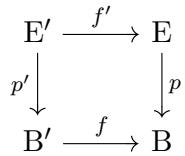
\includegraphics[keepaspectratio]{images/part003_c1a9b5e7.jpg}}

为一个笛卡尔方块。我们假设映射 f 是逆紧、分离且满射的，并作出下列假设之一：

\begin{enumerate}
\def\labelenumi{(\roman{enumi})}
\item
  f 的纤维是局部连通的，且纤维方块 \(B^{\prime} \times_{B} B^{\prime}\) 是局部连通的。
\item
  \(f\) 的纤维是有限的，\(\Delta_{\mathrm{B}^{\prime}}\) 是 \(\mathrm{B}^{\prime}\times_{\mathrm{B}}\mathrm{B}^{\prime}\) 的对角线，且在 \(\mathrm{B}^{\prime}\times_{\mathrm{B}}\mathrm{B}^{\prime}\) 中是开集，并且 \(\mathrm{B}^{\prime}\times_{\mathrm{B}}\mathrm{B}^{\prime} - \Delta_{\mathrm{B}^{\prime}}\) 是局部连通空间。
\end{enumerate}

那么，若 \((\mathrm{E}^{\prime}, p^{\prime})\) 是覆叠，\((\mathrm{E}, p)\) 也是覆叠。

由于映射 \(f\) 是万有严格的（I, 第~20~页，推论），映射 \(p\) 是平展的（I, 第~31~页，命题 8）且分离的（I, 第~27~页，命题 4）。不妨设 \(\mathrm{E}' = \mathrm{B}' \times_{\mathrm{B}} \mathrm{E}\)。

设 \(a\) 是 B 中一点；目标是证明点 \(a\) 有一个邻域 W，使得 W-空间 \((\mathrm{E_W}, p_{\mathrm{W}})\) 是可平凡化的覆叠。令 \(\mathrm{B}_a^\prime = f^{-1}(a)\)，并令 \(\mathrm{E}_a^\prime = (p')^{-1}(\mathrm{E}_a)\)。映射 \(t_a: \mathrm{E}_a^\prime \to \mathrm{B}_a^\prime \times \mathrm{E}_a\) 由 \(t_a(y) = (p'(y), f'(y))\) 定义，是一个 \(\mathrm{B}_a^\prime\)-同构（I, 第~9~页，命题 4），因此 \(\mathrm{E}_a^\prime\) 是 \(\mathrm{B}_a^\prime\) 的可平凡化覆叠，而 \(t_a\) 是此覆叠的平凡化。

证明存在一个邻域 \(V'\)，它是 \(B'_{a}\) 在 \(B'\) 中的邻域，以及覆叠（\(E_{V'}', p_{V'}\)）的一个连续平凡化 t，使其延拓 \(t_{a}\)。在假设（ii）下，\(B'_{a}\) 是有限的，且其中各点有两两不交的开邻域，在这些邻域上覆叠 \(E'\) 可平凡化，故此情形下断言成立。在假设（i）下，\(B'_{a}\) 是局部连通的，B' 也是如此（IV, 第~390~页，引理 1）；由于映射 f 逆紧且分离，\(B'_{a}\) 是紧的，且任意两个不同的点在 B' 中有不交邻域，从而偶对（B', \(B'_{a}\)）满足性质（PCV）（I, 第~37~页，引理 1）。因此断言由 I, 第~90~页推论 2 得出。

由于 \(f\) 逆紧，存在一个邻域 \(V\)，它是 \(a\) 在 \(B\) 中的邻域，使得 \(V'\) 包含 \(f^{-1}(V)\)（I, 第~75~页，引理）。因此不妨设 \(V' = f^{-1}(V)\)。

给 \(V'\)-空间 \(V' \times E_{a}\) 和 \(E_{V'}' = V' \times_{B} E\) 赋予关于 \(f_{V}: V' \to V\) 的规范下降数据。我们要证明，可能缩小 V 和 \(V'\) 后，刚定义的 \(V'\)-空间同构 \(t: E_{V'}' \to V' \times E_{a}\) 与下降数据相容，即有 \(t(b_{1}', x) = t(b_{2}', x)\)，只要 \((b_{1}', b_{2}') \in V' \times_{V} V'\) 且 \(x \in E_{f(b_{1}')}\)。记 \(\widetilde{t}\) 为映射 \(pr_{2} \circ t: E_{V'}' \to E_{a}\)。

令 \(V'' = V' \times_{V} V'\)；通过第一投影将其视为 \(V'\)-空间。映射 \(((b_{1}', b_{2}'), x) \mapsto ((b_{1}', b_{2}'), (b_{1}', x))\)，从 \(V'' \times_{V} E\) 到 \(V'' \times_{V'} E'\)，是 \(V''\)-空间的同构；这说明 \(V'' \times_{V} E\) 是 \(V''\) 的覆叠。

对 \(i=1,2\)，定义映射 \(u_{i}\colon V^{\prime\prime}\times_{V}E\to V^{\prime\prime}\times E_{a}\)，令 \(u_{i}(b_{1}^{\prime},b_{2}^{\prime},x)=(b_{1}^{\prime},b_{2}^{\prime},\widetilde{t}(b_{i}^{\prime},x))\)；它们是覆叠 \(V^{\prime\prime}\times_{V}E\) 的平凡化。令 \(W^{\prime\prime}\) 为点 \(w\in V^{\prime\prime}\) 的集合，在这些点上平凡化 \(u_{1}\) 和 \(u_{2}\) 重合；它包含 \(B_{a}^{\prime}\times B_{a}^{\prime}\)，也包含对角线 \(\Delta_{V'}\)。证明 \(W^{\prime\prime}\) 是 \(B_{a}^{\prime}\times B_{a}^{\prime}\) 的一个邻域。在假设（i）下，这由 I, 第~80~页推论 2 得出，因为 \(B^{\prime}\times B^{\prime}\) 是局部连通的。在假设（ii）下，\(W^{\prime\prime}\) 包含 \((B_{a}^{\prime}\times B_{a}^{\prime})-\Delta_{B_{a}^{\prime}}\) 在 \((B^{\prime}\times_{B}B^{\prime})-\Delta_{B^{\prime}}\) 中的一个邻域，因为这个集合是局部连通的（同上）。由于 \(\Delta_{V'}\) 在 \(B^{\prime}\times_{B}B^{\prime}\) 中开，\(W^{\prime\prime}\) 是 \(B_{a}^{\prime}\times B_{a}^{\prime}\) 在 \(V^{\prime\prime}\) 中的一个邻域。

由于 \(f\) 逆紧，规范映射 \(f''\) 将 \(\mathrm{B}' \times_{\mathrm{B}} \mathrm{B}'\) 映到 B，并且是逆紧的，因为它是投影 \(\mathrm{pr}_{1} \colon \mathrm{B}' \times_{\mathrm{B}} \mathrm{B}' \to \mathrm{B}'\) 与映射 \(f\) 的复合。

根据 I, 第~75~页的引理，存在 V 中 a 的一个邻域 W，使得 \((f'')^{-1}(\mathrm{W})\) 包含于 \(W''\)；令 \(W'=(f')^{-1}(\mathrm{W})\)，它是 \(V'\) 的子集，且平展空间同构 \(t: E_{W'}' \to W' \times E_a\) 与关于映射 \(f_W: W' \to W\) 的规范下降数据相容。根据推论（IV, 第~388~页），

W-平展空间 \(E_{W}\) 和 \(W \times E_{a}\) 同构。特别地，\(E_{W}\) 是可平凡化覆叠，命题得证。

推论 1. --- 设 E 和 B 是拓扑空间，\(p\colon\mathrm{E}\to\mathrm{B}\) 是连续映射，且 \((\mathrm{A}_{i})_{i\in\mathrm{I}}\) 是 B 的局部有限闭覆盖，使得对每一对 \((i,j)\in\mathrm{I}\times\mathrm{I}, i\neq j\)，交集 \(\mathrm{A}_{i}\cap\mathrm{A}_{j}\) 是局部连通空间。那么，B-空间 \((\mathrm{E},p)\) 是覆叠的必要且充分条件是：对每个 \(i\in\mathrm{I}\)，\(\mathrm{A}_{i} \)-空间 \((p^{-1}(\mathrm{A}_{i}),p_{\mathrm{A}_{i}})\) 是 \(\mathrm{A}_{i}\) 的覆叠。

这个条件是必要的（参见 I, 第~69~页）。反之，令 B' 为族 \((\mathrm{A}_{i})_{i\in\mathrm{I}}\) 的拓扑和空间，令 \(f\colon B'\to B\) 为规范映射。映射 f 是闭的（TG, I, 第~6~页，命题 4）、分离的（I, 第~27~页，注 5），具有有限纤维，因而是逆紧的（TG, I, 第~75~页，定理 1）；它还是满射。对角线 \(\Delta_{B'}\) 等于 \(\bigcup_{i\in I}A_{i}\times_{B}A_{i}\)，所以在 \(B'\times_{B}B'\) 中是开集。最后，空间 \((\mathrm{B}'\times_{\mathrm{B}}\mathrm{B}')-\Delta_{\mathrm{B'}}\) 同胚于族 \((\mathrm{A}_{i}\cap\mathrm{A}_{j})\)、\((i,j)\in\mathrm{I}\times\mathrm{I}\)、\(i\neq j\) 的和空间；因而是局部连通的。命题 6 的假设（ii）得到满足。若对每个 i，\(p^{-1}(\mathrm{A}_{i})\) 是 \(A_{i}\) 的覆叠，则 \(E'\) 是 \(B'\) 的覆叠，故 E 是 B 的覆叠。

推论 2. --- 设 X 和 Y 是拓扑空间，设 \(f\colon X \to Y\) 是逆紧、分离且满射的映射。此外，假设下列假设之一成立：

\begin{enumerate}
\def\labelenumi{(\roman{enumi})}
\item
  f 的纤维以及空间 \(X\times_Y X\) 都是局部连通的；
\item
  \(f\) 的纤维是有限的，\(\Delta_{\mathrm{X}}\) 是 \(\mathrm{X} \times_{\mathrm{Y}} \mathrm{X}\) 的对角线，并且在 \(\mathrm{X} \times_{\mathrm{Y}} \mathrm{X}\) 中是开集，空间 \((\mathrm{X} \times_{\mathrm{Y}} \mathrm{X}) - \Delta_{\mathrm{X}}\) 是局部连通的。于是，关于 \(f\) 在 \(\mathrm{X}\) 的覆叠上的每个下降数据都是有效的，且商空间是 \(\mathrm{Y}\) 的覆叠。
\end{enumerate}

设 Z 是 X 的覆叠，\(\tau\) 是关于 f 在 Z 上的下降数据。根据命题 5（IV, 第~389~页），下降数据 \(\tau\) 是有效的，换言之，图表

\pandocbounded{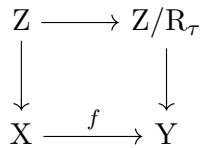
\includegraphics[keepaspectratio]{images/part003_fd3d7e4d.jpg}}

是笛卡尔方形。于是命题 6（IV, 第~391~页）的假设得到满足。因此，\(Z/R_{\tau}\) 是 Y 的覆叠。

命题 7. --- 设 X 和 Y 是拓扑空间，设 \(f: X \to Y\) 是连续且满射的映射。假设 Y 是可解圈的，且映射 f 是开映射并具有道路提升性质。那么，关于 f 在 X 的覆叠上的每个下降数据都是有效的，且商空间是 Y 的覆叠。

设 \((Z,p)\) 是 X 的覆叠，\(\tau\) 是关于 f 在 Z 上的下降数据。由于映射 f 满射且开，根据 IV, 第~389~页命题 5，下降数据 \(\tau\) 是有效的。令 \(T = Y/R_{\tau}\) 表示商 Y-空间；其投影 q 是平展的（同上），也是分离的（I, 第~27~页，命题 4）。

根据假设，映射 f 具有道路提升性质；映射 p 也有，因为 Z 是 X 的覆叠（III, 第~302~页，命题 3 的推论 2）。因此映射 \(p \circ f\) 也具有这一性质，从而映射 q 也有。于是（参见 IV, 第~341~页，注 2），T 是 Y 的覆叠。命题得证。

注。--- 设 X 和 Y 是拓扑空间，设 \(f: X \rightarrow Y\) 是映射。要使关于 f 在 X 的覆叠上的每个下降数据都有效且商空间是 Y 的覆叠，必要条件是 f 严格，并且 \(f(X)\) 是 X 的开闭子集。

事实上，将 X-空间 X 识别为 \(X \times_{Y} Y\)，并赋予它关于 f 的规范下降数据。商空间可识别为 \(f(\mathrm{X})\)，它带有由 f 定义的等价关系下从 X 的拓扑得到的商拓扑。若这是 Y 的覆叠，则空间 \(f(\mathrm{X})\) 可识别为 Y 的开闭子集，而映射 f 是严格的。

\subsection{群胚的下降}

设 X 和 Y 是拓扑空间，设 \(f\colon\mathrm{X}\to\mathrm{Y}\) 是连续映射。设 \(p_{1}\) 和 \(p_{2}\) 是 \(\mathrm{X}\times_{\mathrm{Y}}\mathrm{X}\) 到 X 的两个投影，\(\operatorname{Coeg}(f)\) 是群胚态射对 \((\varpi(p_{1}),\varpi(p_{2}))\) 的余均衡群胚，这两个态射从 \(\varpi(\mathrm{X}\times_{\mathrm{Y}}\mathrm{X})\) 到 \(\varpi(\mathrm{X})\)，而 \(\gamma\colon\varpi(\mathrm{X})\to\operatorname{Coeg}(f)\) 是规范群胚态射（II, 第~199~页，定义 2）。由于 \(f\circ p_{1}=f\circ p_{2}\)，有 \(\varpi(f)\circ\varpi(p_{1})=\varpi(f)\circ\varpi(p_{2})\)。因此根据余均衡子的泛性质（II, 第~199~页，命题 3），存在唯一的群胚态射 \(\varpi'(f)\colon\operatorname{Coeg}(f)\to\varpi(\mathrm{Y})\)，使得 \(\varpi(f)=\varpi'(f)\circ\gamma\)。

Coeg(f) 的顶点集是集合 X = Vert( \(\varpi(X)\) ) 按 f 定义的等价关系所得的商集（II, 第~200~页，注 1）。它可识别为 f(X)。

命题 8. --- 设 X 和 Y 是非空拓扑空间，f 是从 X 到 Y 的连续映射。假设 X 局部道路连通，Y 连通，且 f 严格且满射。那么群胚 Coeg(f) 是传递的。

设 \(\Gamma\) 是这样的箭图：其顶点集为 X，箭集为 \(\mathrm{Fl}(\varpi(\mathrm{X}))\) 与 \(\mathrm{X}\times_{\mathrm{Y}}\mathrm{X}\) 的不交并；源映射和目标映射是 \(\varpi(\mathrm{X})\) 的源映射和目标映射（作用于 \(\mathrm{Fl}(\varpi(\mathrm{X}))\)），以及映射 \(p_1\) 和 \(p_2\)（作用于 \(\mathrm{X}\times_{\mathrm{Y}}\mathrm{X}\)）。根据对 \((\varpi(\mathrm{pr}_1), \varpi(\mathrm{pr}_2))\) 的框架的定义（II, 第~185~页，定义 3）以及 II, 第~200~页注 2，\(\operatorname{Coeg}(f)\) 的轨道集可识别为箭图 \(\Gamma\) 的连通分支集。由于空间 X 非空，只需证明图 \(\Gamma\) 是连通的。

\(\Gamma\) 的连通分支关于等价关系“存在道路连接 \(x\) 与 \(x'\)”是饱和的，因此由于 X 局部道路连通，它们在 X 中是开集。于是它们也是闭集。它们关于 f 定义的等价关系 R 也是饱和的。根据假设，映射 f 诱导出从 X/R 到 Y 的同胚，所以每个 \(\Gamma\) 的连通分支在 f 下的像都是 Y 的开闭子集；由于空间 Y 连通，这个像必为 Y。

设 C 是 \(\Gamma\) 的一个连通分支，设 \(x\) 是 X 中一点。根据前述内容，存在 \(x' \in \mathrm{C}\)，使得 \(f(x') = f(x)\)。根据箭图 \(\Gamma\) 的定义，有 \(x' \in \mathrm{C}\)。因此 \(\mathrm{C} = \mathrm{X}\)，箭图 \(\Gamma\) 从而是连通的。

命题 9. --- 设 X 和 Y 是拓扑空间，f 是从 X 到 Y 的连续映射。假设 X 局部道路连通，Y 是可解圈的，且映射 f 严格且满射。那么，群胚 \(\varpi(\mathrm{Y})\) 由 \(\varpi(\mathrm{X})\) 在 \(\varpi(f)\) 下的像生成。

不妨设空间 X 和 Y 非空。令 G 为 \(\varpi(\mathrm{Y})\) 中由 \(\varpi(\mathrm{X})\) 在 \(\varpi(f)\) 下的像生成的子群胚。由于映射 f 满射，G 的顶点集等于 Y。根据命题 8，\(\operatorname{Coeg}(f)\) 是传递群胚。由于 \(\varpi'(f)\) 在顶点上诱导恒等，\(\operatorname{Coeg}(f)\) 在 \(\varpi'(f)\) 下的像是 \(\varpi(\mathrm{Y})\) 的传递子群胚。\(\varpi(\mathrm{X})\) 在 \(\gamma\) 下的像生成 \(\operatorname{Coeg}(f)\)（II, 第~200~页，推论）；由于有 \(\varpi(f) = \varpi'(f) \circ \gamma\)，群胚 G 是传递的。

设 \(y_{0}\) 是 Y 中一点，令 H 表示子群 \(G_{y_{0}}\)，它是 \(\pi_{1}(Y, y_{0})\) 的子群。根据 IV, 第~342~页定理 1，存在 Y 的连通覆叠（T, p）以及一点 \(t_{0}\)，它属于纤维 \(T_{y_{0}}\)，且其固定子为 H。

若 \(x\) 是 X 中一点，则集合 \(\mathrm{Fl}_{y_0,f(x)}(\mathrm{G})\) 非空，因为 G 是传递的。对于 \(u\in \mathrm{Fl}_{y_0,f(x)}(\mathrm{G})\)，点 \(t_0\cdot u\) 是纤维 \(\mathrm{T}_{f(x)}\) 中的一点，并且与 \(u\) 无关，因为群 H（G 在 \(y_0\) 处的各向同性群）固定 \(t_0\)。将此点记为 \(\sigma (x)\)；将由此定义的映射 \(\sigma \colon \mathrm{X}\to \mathrm{T}\) 记为，并令 \(s\colon \mathrm{X}\to \mathrm{X}\times_{\mathrm{Y}}\mathrm{T}\) 为映射 \(x\mapsto (x,\sigma (x))\)。按构造，映射 s 与 \(\varpi (\mathrm{X})\) 在 X 和 \(\mathrm{X}\times_{\mathrm{Y}}\mathrm{T}\) 上的规范作用相容。由 III, 第~312~页引理 1，s 是连续的。因此映射 \(\sigma\) 连续；此外，由于 \(\sigma (x)\) 只依赖于 \(f(x)\)，它与 f 定义的等价关系相容。由于 f 严格且满射，存在唯一连续映射 \(\overline{\sigma}\colon \mathrm{Y}\to \mathrm{T}\)，使得 \(\overline{\sigma}\circ f = \sigma\)，所以覆叠 T 有截面。由于 T 连通，映射 \(p\colon \mathrm{T}\to \mathrm{Y}\) 是同胚（I, 第~31~页，命题 6 的推论 4），并且 \(\mathrm{H} = \pi_1(\mathrm{Y},y_0)\)，从而 \(\mathrm{G}_{y_0} = \pi_1(\mathrm{Y},y_0)\)。由于 G 传递，得到 \(\mathrm{G} = \varpi (\mathrm{Y})\)。

命题 10. --- 设 X 和 Y 是拓扑空间，f 是从 X 到 Y 的连续映射。假设空间 X 是可解圈的，空间 \(X\times_{Y}X\) 局部道路连通，并且关于 f 在 X 的覆叠上的每个下降数据都是有效的，商空间是 Y 的覆叠。那么群胚态射 \(\varpi'(f)\) 从 Coeg(f) 到 \(\varpi(Y)\)，是单射。

在命题的假设下，\(f\) 是严格的（IV, 第~394~页，注）；此外不妨设它是满射的。

引理 2. --- 保持命题的记号和假设。设 T 是一个集合，赋予它相对于映射 q: T → Y 的群胚 Coeg(f) 作用。那么 T 上存在唯一拓扑，使得 q 使 T 成为 Y 的覆叠，并且对于以 X 中 c 为起点的每个道路类以及 T 中每个点 t，都有 \(t \cdot \gamma(c) = t \cdot f_{*}(c)\)。特别地，Coeg(f) 在 T 上的作用可通过群胚 \(\varpi(Y)\) 的作用分解。

这种 T 上拓扑的唯一性由 III, 第~312~页引理 1 得出；证明其存在性。给集合 \(X\times_{Y}T\) 赋予 \(\varpi(\mathrm{X})\) 的作用，规定 \((x,t)\cdot u=(x\cdot u,t\cdot\gamma(u))\)，其中 \((x,t)\in\mathrm{X}\times_{\mathrm{Y}}\mathrm{T}\)，且 u 是 \(\varpi(\mathrm{X})\) 中源为 x 的每个箭。由于空间 X 是可解圈的，此作用没有局部单值性（III, 第~313~页，注）。因此，在集合 \(X\times_{Y}T\) 上存在唯一拓扑，使 X-空间 \((\mathrm{X}\times_{\mathrm{Y}}\mathrm{T},\mathrm{pr}_{1})\) 成为 X 的覆叠，并使 \(\varpi(\mathrm{X})\) 在此覆叠上的规范作用与给定作用重合（III, 第~313~页，命题 3）。记此覆叠为 \((Z,p)\)。证明映射 \(\tau: ((x_{1},t),x_{2})\mapsto(x_{2},t)\)，从 \(Z\times_{Y}X\) 到 Z，是关于映射 f 在 Z 上的下降数据。只需验证它连续，IV, 第~382~页定义 1 的其他条件显然成立。

映射 \(\tau\) 是映射 \(\mathrm{pr}_2\colon Z\times_Y X\to X\) 到覆叠 \(Z\)（其底空间为 \(X\)）的提升。由于空间 \(X\times_Y X\) 局部道路连通，作为它的覆叠的空间 \(Z\times_Y X\) 也局部道路连通。根据推论（III, 第~269~页），要证明映射 \(\tau\) 连续，只需证明它沿道路连续。

设 \(\widetilde{c} = ((c,g),c')\) 是 \(Z\times_{Y}X\) 中的一条道路，证明映射 \(\tau \circ \widetilde{c}\colon t\mapsto (c'(t),g(t))\) 从 I 到 Z 连续。对于每个 \(s\in [0,1]\)，记 \(c_s\) 和 \(c_s'\) 为 X 中分别由 \(t\mapsto c(st)\) 和 \(t\mapsto c'(st)\) 定义的道路。对于所有 \(s\in [0,1]\)，于是有 \(c(s) = c(0)\cdot [c_s]\)、\(c'(s) = c'(0)\cdot [c_s']\) 以及 \((c,g)(s) = (c(0),g(0))\cdot [c_s]\)，其中 \([u]\) 表示道路 u 的严格同伦类（III, 第~304~页，注）。映射 \(t\mapsto (c_s(t),c_s'(t))\) 是 \(X\times_{Y}X\) 中的一条道路；根据余均衡群胚 Coeg(f) 的定义，有 \(\gamma ([c_s]) = \gamma ([c_s'])\)，并且 \(g(s) = g(0)\cdot \gamma ([c_s]) = g(0)\cdot \gamma ([c_s'])\)。根据 \(\varpi (X)\) 在 Z 上的作用定义，因而有

\[
\begin{array}{r} (\tau \circ \widetilde {c}) (s) = (c ^ {\prime} (s), g (s)) = (c ^ {\prime} (0) \cdot [ c _ {s} ^ {\prime} ], g (0) \cdot \gamma ([ c _ {s} ^ {\prime} ])) \\ = (c ^ {\prime} (0), g (0)) \cdot [ c _ {s} ^ {\prime} ] = (\tau \circ \widetilde {c}) (0) \cdot [ c _ {s} ^ {\prime} ]. \end{array}
\]

这说明 \(\tau \circ \widetilde{c}\) 是道路 \(c'\) 到 Z 的连续提升（同上）。因此，映射 \(\tau\) 沿道路连续，因而连续；它是 X-空间 Z 关于 \(f\) 的下降数据。

记 \(R_{\tau}\) 为下降数据 \(\tau\) 定义的等价关系。由于映射 f 满射，映射 \(pr_{2}: Z \to T\) 通过取商诱导出从 \(Z/R_{\tau}\) 到 T 的双射。通过结构传递，将由 \(Z/R_{\tau}\) 的拓扑得到的拓扑赋予 T，使得 \((T,q)\) 成为 Y-空间。根据假设，T 因而是 Y 的覆叠，且图表

\[
\begin{array}{c} \mathrm{Z} \xrightarrow {\mathrm{pr} _ {2}} \mathrm{T} \\ p \Big \downarrow \qquad \qquad \qquad \qquad \Big \downarrow q \\ \mathrm{X} \xrightarrow {f} \mathrm{Y} \end{array}
\]

是笛卡尔方形。

设 \((x,t)\) 是 Z 中一点，设 c 是 X 中以 x 为起点的一条道路，并设 \(\widetilde{c}\) 是以 \((x,t)\) 为起点的 c 到 Z 的连续提升。道路 \(pr_{2} \circ \widetilde{c}\) 是道路 \(f \circ c\) 在 Y 中以 t 为起点的提升，因此 \(t \cdot \gamma([c]) = t \cdot [f \circ c] = t \cdot f_{*}([c])\)。引理得证。

现在证明命题。设 \(u\) 和 \(v\) 是 Coeg( \(f\) ) 的两个箭，它们在 \(\varpi(Y)\) 中的像相等。由于群胚态射 \(\varpi'(f)\) 在顶点集上是恒等的，箭 \(u\) 和 \(v\) 有相同的起点和终点。记 \(y\) 为 \(u\) 的起点；令 T 为 Coeg( \(f\) ) 中以 y 为源的箭集，并令 \(q: \mathrm{T} \to \mathrm{Y}\) 为目标映射在 T 上的限制。群胚 Coeg( \(f\) ) 关于 \(q\) 通过右合成作用于集合 T。根据引理 2，\(u\) 和 \(v\) 在 T 上的作用相同。因此有 \(u = e_y \cdot u = e_y \cdot v = v\)。这证明群胚态射 \(\varpi'(f)\) 是单射。

定理 1. --- 设 X 和 Y 是拓扑空间，设 \(f: X \to Y\) 是连续且满射的映射。假设空间 X 和 Y 都是可解圈的。最后，假设下列性质之一成立：

\begin{enumerate}
\def\labelenumi{(\roman{enumi})}
\item
  映射 f 逆紧、分离，具有局部连通的纤维，且空间 \(X\times_{Y}X\) 局部道路连通；
\item
  映射 f 逆紧、分离，具有有限纤维，对角线 \(\Delta_{X}\) 在 \(X \times_{Y} X\) 中是开集，且其补集是局部连通的；
\item
  映射 f 是开映射并具有道路提升性质。
\end{enumerate}

那么，群胚态射 \(\varpi'(f)\) 是从群胚 Coeg(f) 到庞加莱群胚 \(\varpi(Y)\) 的同构。

首先注意，在这些假设下，映射 \(f\) 是满射且严格的（I, 第~18~页，例 2）。此外，关于 \(f\) 在 X 的覆叠上的每个下降数据都是有效的，商空间是 Y 的覆叠；这在假设（i）和（ii）下由 IV, 第~393~页命题 4 的推论 2 得出，在假设（iii）下由 IV, 第~394~页命题 7 得出。根据命题 10，群胚态射 \(\varpi'(f)\) 因而是单射，且其像是 \(\varpi(Y)\) 的子群胚。

根据 IV, 第~395~页命题 9，在假设（i）和（ii）下，此像等于 \(\varpi(\mathrm{Y})\)；在假设（iii）下也如此，因为此时群胚态射 \(\varpi(f)\) 是满射的。

因此，\(\varpi'(f)\) 是同构。

例。--- 下面是两个满足定理 1 假设的例子。

\begin{enumerate}
\def\labelenumi{\arabic{enumi})}
\item
  设 Y 是可解圈拓扑空间。设 \((\mathrm{A}_{i})_{i\in\mathrm{I}}\) 是由闭集构成的 Y 的局部有限覆盖。假设对每个 \(i\in I\)，空间 \(A_{i}\) 是可解圈的，并且对每一对 \((i,j)\in\mathrm{I}\times\mathrm{I}\)，空间 \(A_{i}\cap A_{j}\) 局部道路连通。可以取 X 为族 \((\mathrm{A}_{i})_{i\in\mathrm{I}}\) 的和空间，取 \(f:X\to Y\) 为由规范嵌入族导出的映射。
\item
  设 G 是作用在可解圈拓扑空间 X 上的离散群，且作用是适当的；令 Y = X/G，并令 \(f: X \to Y\) 为规范映射。它是开映射（TG, III, 第~10~页，引理 2），并根据 III, 第~287~页定理 4 具有道路提升性质。根据 IV, 第~349~页命题 8 b)，空间 Y 是可解圈的。由从 G × X 到 \(X\times X\) 的映射 \((g, x) \mapsto (g \cdot x, x)\) 给出的映射是逆紧的，因而严格（I, 第~18~页，例 2），且其像是 \(X\times_{Y}X\)。于是根据 III, 第~261~页命题 8，\(X\times_{Y}X\) 局部道路连通。
\end{enumerate}

\subsection{通过平展且满射的映射下降}

设 X 和 Y 是拓扑空间，f 是从 X 到 Y 的连续映射。沿用前一节的记号。

定理 2. --- 假设 Y 的每一点都有一个邻域，在其上存在映射 f 的连续截面。那么，群胚态射 \(\varpi'(f)\) 是从 \(\operatorname{Coeg}(f)\) 到 \(\varpi(Y)\) 的同构。

根据假设，存在由开集构成的 Y 的覆盖 \((\mathrm{U}_{j})_{j\in\mathrm{J}}\)，并且对每个 \(j\in J\)，有连续截面 \(s_{j}\)，它是 \(f_{U_{j}}\) 的截面。

若 \(c\) 是 X 中的一条道路，我们将 \([c]\) 记为它在 \(\varpi(X)\) 中的严格同伦类，将 \(\{c\}\) 记为 \([c]\) 在 \(\operatorname{Coeg}(f)\) 中经群胚态射 \(\gamma\) 得到的像。若 \(c\) 和 \(c'\) 是 X 中的两条道路，则 \(\{c\}\) 和 \(\{c'\}\) 在 \(\operatorname{Coeg}(f)\) 中可合成，当且仅当道路 \(f \circ c\) 和 \(f \circ c'\) 在 Y 中可首尾相接。

设 \(c'\) 是 Y 中的一条道路。根据 III, 第~272~页引理 4，将其应用于紧空间 I 以及 I 的覆盖 \(((c')^{-1}(\mathrm{U}_j))_{j\in \mathrm{J}}\)，存在整数 \(n\)，使得对每个整数 \(k\)，若满足 \(1\leqslant k\leqslant n\)，则区间 \([\frac{k - 1}{n},\frac{k}{n}]\) 在 \(c'\) 下的像包含于某个开集 \(\mathrm{U}_{j(k)}\) 中。对每个整数 \(k\)，若 \(1\leqslant k\leqslant n\)，令 \(c_k'\) 为 Y 中由 \(s\mapsto c'(\frac{k + s - 1}{n})\) 定义的道路；有 \([c'] = [c_1'][c_2']\ldots [c_n']\)（参见 III, 第~291~页，注 1），且 \(c'\) 就是记作 \(c_1' * c_2' * \dots * c_n'\) 的道路。对所有 \(k\in \{1,\ldots ,n\}\)，记 \(c_k\) 为 X 中的道路 \(s_{j(k)}\circ c_k'\)，并置 \(\{c_k\} = \gamma ([c_k])\)。由于对每个 \(k\)，道路 \(c_{k - 1}' = f\circ c_{k - 1}\) 和 \(c_k' = f\circ c_k\) 可首尾相接，序列 \((\{c_1\} ,\ldots ,\{c_n\})\) 在 \(\operatorname{Coeg}(f)\) 中可合成。由构造，

\[
\begin{array}{r l} & {\varpi^ {\prime} (f) (\{c _ {1} \} \ldots \{c _ {n} \}) = \varpi^ {\prime} (f) (\{c _ {1} \}) \ldots \varpi^ {\prime} (f) (\{c _ {n} \})} \\ & {\qquad = \varpi (f) ([ c _ {1} ]) \ldots \varpi (f) ([ c _ {n} ])} \\ & {\qquad = [ f \circ c _ {1} ] \ldots [ f \circ c _ {n} ]} \\ & {\qquad = [ c _ {1} ^ {\prime} ] * \dots * [ c _ {n} ^ {\prime} ] = [ c ^ {\prime} ],} \end{array}
\]

这证明群胚态射 \(\varpi'(f)\) 是满射。

设 \(u\) 和 \(v\) 是 \(\operatorname{Coeg}(f)\) 的箭。由于群胚 \(\operatorname{Coeg}(f)\) 由 \(\varpi(\mathrm{X})\) 的像生成（II, 第~200~页，推论），存在 X 中道路的有限序列 \((c_1, \ldots, c_n)\) 和 \((d_1, \ldots, d_n)\)，使得 \(u = \{c_1\} \ldots \{c_n\}\) 且 \(v = \{d_1\} \ldots \{d_n\}\)。道路 \((f \circ c_1, \ldots, f \circ c_n)\) 在 Y 中可首尾相接，并且有 \(\varpi'(f)(u) = [(f \circ c_1)] \ldots [(f \circ c_n)]\)；同样，\(\varpi'(f)(v) = [(f \circ d_1)] \ldots [(f \circ d_n)]\)。

假设有 \(\varpi'(f)(u) = \varpi'(f)(v)\)。于是存在严格同伦 \(\sigma\)，连接 \((f \circ c_1) * \cdots * (f \circ c_n)\) 与 \((f \circ d_1) * \cdots * (f \circ d_n)\)。根据 III, 第~272~页引理 4，将其应用于紧空间 \(\mathbf{I} \times \mathbf{I}\) 以及覆盖 \((\bar{\sigma}^{-1}(\mathrm{U}_i))_{i \in \mathrm{I}}\) 的空间 \(\mathbf{I} \times \mathbf{I}\)，存在整数 \(m \geqslant 1\)，使得对每一对整数 \((j,k)\)，若满足 \(1 \leqslant j \leqslant m\) 且 \(1 \leqslant k \leqslant m\)，则区间积 \([\frac{j-1}{m}, \frac{j}{m}] \times [\frac{k-1}{m}, \frac{k}{m}]\) 在 \(\sigma\) 下的像包含于某个开集 \(U_{i(j,k)}\) 中，该开集属于覆盖 \((\mathrm{U}_{i})_{i \in \mathrm{I}}\)。

X 中每条道路 c 都形如 \(c_{1}*\cdots*c_{m}\)，其中 \(c_{k}\) 是由 \(t\mapsto c(\frac{k-1+t}{m})\) 定义的道路。如有必要，将整数 m 和 n 换成它们的乘积 mn，因此可以假设 m=n。

对于每一对整数 \((j,k)\)（属于 \(\{1,\ldots ,n\}\)）以及每一对 \((s,t)\in\) \(\mathbf{I}\times \mathbf{I}\)，置

\[
\sigma_ {j, k} (s, t) = s _ {i (j, k)} \circ \sigma \left(\frac {s + j - 1}{n}, \frac {t + k - 1}{n}\right).
\]

对于 \(t \in \mathbf{I}\)，再置 \(h_{j,k}^{0}(t) = \sigma_{j,k}(t,0)\)、\(h_{j,k}^{1}(t) = \sigma_{j,k}(t,1)\)、\(v_{j,k}^{0}(t) = \sigma_{j,k}(0,t)\) 以及 \(v_{j,k}^{1}(t) = \sigma_{j,k}(1,t)\)。根据 III, 第~295~页引理 1，道路 \(h_{j,k}^{0} * v_{j,k}^{1}\) 和 \(v_{j,k}^{0} * h_{j,k}^{1}\) 严格同伦，因此有关系

\[
[ h _ {j, k} ^ {0} ] [ v _ {j, k} ^ {1} ] = [ v _ {j, k} ^ {0} ] [ h _ {j, k} ^ {1} ]\tag{2}
\]

在 \(\varpi(\mathrm{X})\) 上，对每一对 \((j,k) \in \{1, \ldots, n\}^2\) 都成立。另一方面，对每一对整数 \((j,k)\)，若 \(2 \leqslant j \leqslant n\) 且 \(1 \leqslant k \leqslant n\)，有 \(f \circ v_{j,k}^0 = f \circ v_{j-1,k}^1\)，因此有关系

\[
\{v _ {j, k} ^ {0} \} = \{v _ {j - 1, k} ^ {1} \}\tag{3}
\]

在 Coeg(f) 中。类似地，对每一对整数 \((j,k)\)，若 \(1 \leqslant j \leqslant n\) 且 \(2 \leqslant k \leqslant n\)，有

\[
\{h _ {j, k} ^ {0} \} = \{h _ {j, k - 1} ^ {1} \}.\tag{4}
\]

对于 \(j \in \{1, \ldots, n\}\)，道路 \(f \circ c_j\) 和 \(f \circ h_{j,1}^0\) 重合。根据余均衡子 Coeg(f) 的定义，因此有 \(\{c_j\} = \{h_{j,1}^0\}\)。同样，对每个 \(j \in \{1, \ldots, n\}\)，有 \(\{d_j\} = \{h_{j,n}^1\}\)。因此有如下关系

\[
u = \{h _ {1, 1} ^ {0} \} \dots \{h _ {n, 1} ^ {0} \}, \quad v = \{h _ {1, n} ^ {1} \} \dots \{h _ {n, n} ^ {1} \}.
\]

根据下面的引理 3，有

\[
\{h _ {1, 1} ^ {0} \} \dots \{h _ {1, n} ^ {0} \} \{v _ {1, n} ^ {1} \} \dots \{v _ {n, n} ^ {1} \} = \{v _ {1, 1} ^ {0} \} \dots \{v _ {n, 1} ^ {0} \} \{h _ {n, 1} ^ {1} \} \dots \{h _ {n, n} ^ {1} \}.
\]

由于道路 \(t \mapsto \sigma(0,t)\) 和 \(t \mapsto \sigma(1,t)\) 是常值，对 \(1 \leqslant k \leqslant n\)，有 \(\{v_{1,k}^{0}\} = e_{a}\) 且 \(\{v_{n,k}^{1}\} = e_{b}\)，其中 \(a,b \in Y\) 是箭 \(u\) 和 \(v\) 的起点和终点，它们属于群胚 Coeg( \(f\) )。因此有等式

\[
\{h _ {1, 1} ^ {0} \} \dots \{h _ {1, n} ^ {0} \} = \{h _ {n, 1} ^ {0} \} \dots \{h _ {n, n} ^ {1} \},
\]

即 u = v。

引理 3. --- 设 G 是群胚，p、q 是满足 \(\geqslant 1\) 的整数。对于每一对整数 \((j, k)\)，若 \(0 \leqslant j \leqslant p\) 且 \(0 \leqslant k \leqslant q\)，令 \(x_{j,k}\) 为 G 的一个顶点；对于每一对整数 \((j, k)\)，若 \(1 \leqslant j \leqslant p\) 且 \(0 \leqslant k \leqslant q\)，令 \(h_{j,k}\) 为连接 \(x_{j-1,k}\) 与 \(x_{j,k}\) 的 G 的一个箭；对于每一对整数 \((j, k)\)，若 \(0 \leqslant j \leqslant p\) 且 \(1 \leqslant k \leqslant q\)，令 \(v_{j,k}\) 为连接 \(x_{j,k-1}\) 与 \(x_{j,k}\) 的 G 的一个箭。

假设对于每一对整数 \((j,k)\)，若 \(1 \leqslant j \leqslant p\) 且 \(1 \leqslant k \leqslant q\)，箭 \(v_{j-1,k}\) 和 \(h_{j,k}\) 可合成，箭 \(h_{j,k-1}\) 和 \(v_{j,k}\) 也可合成，并且有 \(v_{j-1,k}h_{j,k} = h_{j,k-1}v_{j,k}\)。那么，

\[
h _ {1, 0} h _ {2, 0} \dots h _ {p, 0} v _ {p, 1} v _ {p, 2} \dots v _ {p, q} = v _ {0, 1} v _ {0, 2} \dots v _ {0, q} h _ {1, q} h _ {2, q} \dots h _ {p, q}.
\]

先处理 q = 1 的特殊情形，并对 p 作归纳证明。若 p = 1，待证断言由假设得到验证；假设它对 p - 1 成立；于是有

\[
h _ {1, 0} h _ {2, 0} \dots h _ {p, 0} v _ {p, 1} = h _ {1, 0} h _ {2, 0} \dots h _ {p - 1, 0} v _ {p - 1, 1} h _ {p, 1} = v _ {0, 1} h _ {1, 1} \dots h _ {p, 1}
\]

根据归纳假设，从而得到 p 的关系。

现在对 q 作归纳证明。根据前述内容，q = 1 时命题成立；若对 q - 1 成立，则有

\[
h _ {1, 0} h _ {2, 0} \dots h _ {p, 0} v _ {p, 1} v _ {p, 2} \dots v _ {p, q} = v _ {0, 1} v _ {0, 2} \dots v _ {0, q - 1} h _ {1, q - 1} \dots h _ {p, q - 1} v _ {p, q}.
\]

根据 \(q = 1\) 的情形，有

\[
h _ {1, q - 1} \dots h _ {p, q - 1} v _ {p, q} = v _ {0, q} h _ {1, q} \dots h _ {p, q},
\]

从而得到所需关系。

例。--- 1) 当映射 f 平展且满射时，定理适用。

\begin{enumerate}
\def\labelenumi{\arabic{enumi})}
\setcounter{enumi}{1}
\tightlist
\item
  它也适用于如下情形：空间 X 是集合族 \((V_{i})_{i\in\mathrm{I}}\) 的和空间，其中这些 Y 的子集的内部覆盖 Y，且 f 是由每个 \(V_{i}\) 到 Y 的规范嵌入导出的映射。
\end{enumerate}

\subsection{商空间的庞加莱群胚}

设 X 是赋予离散群 G 连续作用的拓扑空间；令 Y = X/G，并将 \(f: X \to Y\) 记为规范映射。记 \(\lvert G\rvert\) 为群胚 \(\varpi(G)\)；其顶点集为 G；对于 \(g, g' \in G\)，存在从 g 到 \(g'\) 的唯一箭，当且仅当 \(g' = g\)，否则不存在。通过取基本群胚，作用 \(m: G \times X \to X\) 诱导出群胚态射 \(\varpi(m): \lvert G\rvert \times \varpi(X) \to \varpi(X)\)。令 \(\varpi(X)/G\) 为群胚态射 \(\varpi(m)\) 和 \(\varpi(\mathrm{pr}_{2})\) 的余均衡子，这两个态射从 \(\lvert G\rvert \times \varpi(X)\) 到 \(\varpi(X)\)；记 \(\beta: \varpi(X) \to \varpi(X)/G\) 为规范群胚态射。我们有 \(f \circ m = f \circ pr_{2}\)，因此 \(\varpi(f) \circ \varpi(m) = \varpi(f) \circ \varpi(\mathrm{pr}_{2})\)。根据余均衡子的泛性质，存在唯一群胚态射 \(\varpi''(f): \varpi(X)/G \to \varpi(Y)\)，使得 \(\varpi(f) = \varpi''(f) \circ \beta\)。

定理 3. --- 设 X 是可解圈拓扑空间，G 是适当地作用于 X 的离散群；设 \(f\colon X \to X/G\) 为规范满射。上面引入的规范群胚态射 \(\varpi''(f)\colon \varpi(X)/G \to \varpi(X/G)\) 是同构。

记 \(\operatorname{Coeg}(f)\) 为从 \(\varpi(\mathrm{X} \times_{\mathrm{Y}} \mathrm{X})\) 到 \(\varpi(\mathrm{X})\) 的两个群胚态射的余均衡子，这两个态射由投影 \(pr_{1}\) 和 \(pr_{2}\) 诱导；令 \(\gamma: \varpi(\mathrm{X}) \to \operatorname{Coeg}(f)\) 为规范群胚态射。由于映射 \((m, pr_{2})\) : \(G \times X \to X \times X\) 的像是 \(X \times_{Y} X\) 在 \(X \times X\) 中的子空间，群胚态射 \(\gamma \circ \varpi(m)\) 和 \(\gamma \circ \varpi(pr_{2})\)（从 \(\lvert G\rvert \times \varpi(X)\) 到 \(\operatorname{Coeg}(f)\)）相等。根据 \(\varpi(\mathrm{X})/\mathrm{G}\) 的泛性质，存在唯一群胚态射 \(\alpha: \varpi(\mathrm{X})/\mathrm{G} \to \operatorname{Coeg}(f)\)，使得 \(\gamma = \alpha \circ \beta\)。

我们也将唯一的群胚态射 \(\varpi'(f)\) 记为从 \(\operatorname{Coeg}(f)\) 到 \(\varpi(Y)\) 且满足 \(\varpi(f) = \varpi'(f) \circ \gamma\) 的态射。根据 IV, 第~399~页，例 2，IV, 第~398~页定理 1 的假设得到满足，且态射 \(\varpi'(f)\) 是同构。由于

\[
\varpi (f) = \varpi^ {\prime} (f) \circ \gamma = \varpi^ {\prime} (f) \circ \alpha \circ \beta = \varpi^ {\prime \prime} (f) \circ \beta ,
\]

有 \(\varpi''(f) = \varpi'(f) \circ \alpha\)。因此，要证明定理 3，只需证明态射 \(\alpha\) 是同构。

引理 4. --- 对每条道路 \(c = (c_1, c_2)\)，若其属于 \(X \times_Y X\)，则有 \(\beta([c_1]) = \beta([c_2])\)。

设 c 是这样的一条道路。

设 \(x \in X\)，令 \(K_x\) 为 x 在 G 中的稳定子。根据 TG, III, 第~32~页命题 8，存在一个开邻域 \(U_x\)，它是 \(x\) 在 X 中的邻域，使得 \(K_x \cdot U_x = U_x\)，

\(g \cdot U_x \cap U_x = \varnothing\) 对所有 \(g \in G - K_x\) 成立，并且映射 f 诱导出从 \(U_x/K_x\) 到 Y 中开邻域 \(V_x\) 的同胚，其中包含 \(f(x)\)。由于 X 是可解圈的，且映射 f 在 \(U_x\) 上的限制是开且闭的，不妨进一步假设 \(U_x\) 是连通的，并且规范同态 \(\pi_1(U_x, x) \to \pi_1(X, x)\) 的像化为单位元。这样构造的开集 \((V_x)_{x \in X}\) 构成 Y 的一个开覆盖。根据 III, 第~272~页引理 4，将其应用于紧空间 I 以及开集 \((f \circ c_1)^{-1}(V_x)\)（\(x \in X\)），存在整数 \(n \geqslant 1\)，使得对每个 \(i \in \{1, \ldots, n\}\)，存在 X 中一点 \(x_i\)，使得 \(c_1([i-1/n, i/n])\) 包含于 \(f(V_{x_i})\)。由于 \(f \circ c_1 = f \circ c_2\)，\(c_2([i-1/n, i/n])\) 也包含于 \(f(V_{x_i})\)。

对于 \(j = 1\) 或 2 以及 \(i \in \{1, \ldots, n\}\)，记 \(c_{j,i}\) 为 X 中由 \(t \mapsto c_j(\frac{i+t-1}{n})\) 定义的道路；有 \(c_j = c_{j,1} * \cdots * c_{j,n}\)（III, 第~291~页，注 1）。因此，要证明 \(\beta([c_1]) = \beta([c_2])\)，只需证明 \(\beta([c_{1,i}]) = \beta([c_{2,i}])\)，对每个整数 \(i \in \{1, \ldots, n\}\) 都如此。将道路 \((c_1, c_2)\) 替换为道路 \((c_{1,i}, c_{2,i})\)，于是可假设存在 \(x \in X\)，使得 \((f \circ c_1)([0,1]) \subset V_x\)。

\(V_{x}\) 在 f 下的逆像是连通分支 \(g \cdot U_{x}\) 的不交并，其中 g 遍历 G 中 \(G/K_{x}\) 的一组代表。对于 i = 1 或 2，取 G 中元素 \(g_{i}\)，使得点 \(x_{i} = g_{i} \cdot c_{i}(0)\) 属于 \(U_{x}\)。于是道路 \(g_{i} \cdot c_{i}\) 的像包含于 \(U_{x}\)。根据群胚 \(\varpi(\mathrm{X})/\mathrm{G}\) 的定义，有 \(\beta([g_{i} \cdot c_{i}]) = \beta([c_{i}])\)，从而可以假设道路 \(c_{1}\) 和 \(c_{2}\) 的像包含于 \(U_{x}\)，且 \(g_{1} = g_{2} = e\)。

对于 \(s=0\) 或 1，令 \(d_{s}\) 为 \(\mathrm{U}_{x}\) 中连接 \(x\) 与 \(c_{1}(s)\) 的道路，并令 \(g_{s}\) 为 \(\mathrm{K}_{x}\) 中满足 \(g_{s}\cdot c_{2}(s)=c_{1}(s)\) 的元素。道路 \(d_{0}*c_{1}*\overline{d_{1}}\) 和 \(d_{0}*(g_{0}\cdot c_{2})*(g_{0}g_{1}^{-1}\cdot\overline{d_{1}})\) 是以 \(x\) 为基点、位于 \(\mathrm{U}_{x}\) 中的圈。因此，它们在 X 中都严格同伦于以 \(x\) 为基点的常值圈，因为规范同态 \(\pi_{1}(\mathrm{U}_{x},x)\to\pi_{1}(\mathrm{X},x)\) 的像化为单位元。尤其，它们的类在群胚态射 \(\beta\) 下有相同的像，于是

\[
\beta ([ d _ {0} ]) \beta ([ c _ {1} ]) \beta ([ d _ {1} ]) ^ {- 1} = \beta ([ d _ {0} ]) \beta ([ g _ {0} \cdot c _ {2} ]) \beta ([ g _ {0} g _ {1} ^ {- 1} \cdot d _ {1} ]) ^ {- 1}.
\]

由于 \(\beta([g \cdot c]) = \beta([c])\) 对每个元素 \(g \in G\) 以及每条道路 \(c\)，它位于 \(X\) 中，都成立，故有 \(\beta([c_1]) = \beta([c_2])\)，引理得证。

根据引理，两个群胚态射 \(\beta \circ \varpi(\mathrm{pr}_{1})\) 和 \(\beta \circ \varpi(\mathrm{pr}_{2})\)，它们从 \(\varpi(\mathrm{X} \times_{\mathrm{Y}} \mathrm{X})\) 到 \(\operatorname{Coeg}(f)\)，相等。根据余均衡子的泛性质，因此存在唯一群胚态射 \(\alpha'\)：\(\operatorname{Coeg}(f) \to \varpi(\mathrm{X})/\mathrm{G}\)，使得 \(\beta = \alpha' \circ \gamma\)。态射 \(\alpha' \circ \alpha\) 是唯一的群胚态射 \(\varphi\)，它作用于 \(\varpi(\mathrm{X})/\mathrm{G}\) 并映到自身，且满足 \(\varphi \circ \beta = \beta\)；因此有 \(\alpha' \circ \alpha = \operatorname{Id}_{\varpi(\mathrm{X})/\mathrm{G}}\)。同样，\(\alpha \circ \alpha' = \operatorname{Id}_{\operatorname{Coeg}(f)}\)。所以，\(\alpha\) 是同构。

\section{范坎彭定理}

\subsection{纤维方块投影的余均衡子}

设 X 与 Y 为拓扑空间，f 为从 X 到 Y 的一个连续映射。用 Z 表示纤维方块 \(X \times_{Y} X\)，用 \(p_{1}\) 与 \(p_{2}\) 表示从 Z 到 X 的两个投影。我们用 W 表示纤维积 \(X \times_{Y} X \times_{Y} X\)；对每个偶 \((s, t)\)（由 \(\{1,2,3\}\) 中的元素组成），用 \(q_{st}: W \to Z\) 表示由 \(q_{st}(x_{1}, x_{2}, x_{3}) = (x_{s}, x_{t})\) 定义的映射。

用 \(\operatorname{Coeg}(f)\) 表示群胚 \(\operatorname{Coeg}(\varpi(p_{1}),\varpi(p_{2}))\)，即两个态射 \(\varpi(p_{1})\)、\(\varpi(p_{2})\)（从庞加莱群胚 \(\varpi(Z)\) 到庞加莱群胚 \(\varpi(X)\)）的余均衡子。用 \(\gamma\colon\varpi(X)\to\operatorname{Coeg}(f)\) 表示规范的群胚态射。由于 \(f\circ p_{1}=f\circ p_{2}\)，群胚态射 \(\varpi(f)\circ\varpi(p_{1})\) 与 \(\varpi(f)\circ\varpi(p_{2})\)（从 \(\varpi(Z)\) 到 \(\varpi(Y)\)）相等；因此存在唯一的群胚态射 \(\varpi'(f)\colon\operatorname{Coeg}(f)\to\varpi(Y)\) 使得 \(\varpi'(f)\circ\gamma=\varpi(f)\)。

定义 1. --- 我们说映射 f 满足性质 (VK)，如果它是严格、满射的，并且态射 \(\varpi'(f)\) 是同构。

例 1. --- 在下列假设之一之下，此性质成立：

\begin{enumerate}
\def\labelenumi{(\roman{enumi})}
\item
  空间 X 与 Y 是可解圈的，空间 \(X \times_{Y} X\) 局部道路连通，映射 f 满射、逆紧、分离，且具有局部连通的纤维；
\item
  空间 X 与 Y 是可解圈的，映射 f 满射、逆紧、分离，且具有有限纤维，对角线 \(\Delta_{X}\) 在 \(X \times_{Y} X\) 中是开集且其补集局部连通；
\item
  空间 X 与 Y 是可解圈的，映射 f 满射、开，且具有道路提升性质；
\item
  Y 的每个点都有一个邻域，在该邻域之上存在映射 f 的连续截面。
\end{enumerate}

事实上，在这些假设的每一条之下，映射 \(f\) 都是满射；并且依据 I, 第~18~页，例 2，它也是严格的。最后，态射 \(\varpi'(f)\) 是同构：在假设 (i)、(ii) 或 (iii) 之下依据 IV, 第~398~页，定理 1，在假设 (iv) 之下依据（IV, 第~400~页，定理 2）。

II, 第~208~页的命题 5 描述了群胚 Coeg(f) 的迷向群。本节的目的在于：当 f 满足性质 (VK) 时，明显写出通过与群胚同构 \(\varpi'(f)\) 复合而由此得到的 Y 的庞加莱群的描述。随后的各号将用于讨论重要的特殊情形。

假设映射 f 满足性质 (VK)。

令 \(\mathsf{I} = \pi_0(\mathrm{X})\)，\(\mathsf{J} = \pi_0(\mathrm{Z})\)，\(\mathsf{K} = \pi_0(\mathrm{W})\)；对 \(j \in \mathsf{J}\) 与 \(s \in \{1,2\}\)，令 \(i_s(j) = \pi_0(p_s)(j)\)；对 \(k \in \mathsf{K}\) 与 \(s\)、\(t \in \{1,2,3\}\)，令 \(j_{st}(k) = \pi_0(q_{st})(k)\)。用 \(\Gamma\) 表示群胚态射偶 \((\varpi(p_1), \varpi(p_2))\)（从 \(\varpi(\mathrm{Z})\) 到 \(\varpi(\mathrm{X})\)）的框架（II, 第~185~页，定义 3）。它就是箭图 \((\mathsf{I}, \mathsf{J}, \pi_0(p_1), \pi_0(p_2))\)，因为拓扑空间的庞加莱群胚的轨道就是该空间的道路连通分支。

此外假设 Y 道路连通且非空。由 II, 第~200~页，注 2，\(\pi_0(\Gamma)\) 于是与群胚 Coeg(f) 的轨道集成双射；由于映射 \(f\) 满足性质 (VK)，群胚 Coeg(f) 同构于群胚 \(\varpi(Y)\)。于是图 \(\Gamma\) 连通且非空。

我们把 f 的范坎彭数据称为由下列元素组成的数据：

\begin{enumerate}
\def\labelenumi{(\roman{enumi})}
\item
  对每个 \(i \in \mathsf{I}\)，取 \(\mathsf{a}(i)\) 为道路连通分支 \(i\)（在 \(\mathbf{X}\) 中）的一点；
\item
  对每个 \(j \in J\)，取 Z 的道路连通分支 j 中的一点 \(\mathsf{b}(j) = (\mathsf{b}_{1}(j), \mathsf{b}_{2}(j))\)；
\item
  对每个 \(k \in \mathsf{K}\)，取 \(\mathsf{c}(k) = (\mathsf{c}_1(k), \mathsf{c}_2(k), \mathsf{c}_3(k))\) 为道路连通分支 \(k\)（在 \(\mathbf{W}\) 中）的一点；
\item
  对每个 \(j \in J\)，取 X 中一条道路的类 \(\beta_{1}(j)\)，该道路连接 \(\mathsf{b}_{1}(j)\) 与 \(\mathsf{a}(i_{1}(j))\)；再取 X 中一条道路的类 \(\beta_{2}(j)\)，该道路连接 \(\mathsf{b}_{2}(j)\) 与 \(\mathsf{a}(i_{2}(j))\)；
\item
  对每个 \(k \in K\) 与每个偶 \((s, t)\)（等于 \((1, 2)\)、\((2, 3)\) 或 \((1, 3)\)），取 Z 中一条道路的类 \(\gamma_{st}(k)\)，该道路连接 \((\mathsf{c}_{s}(k), \mathsf{c}_{t}(k))\) 与 \(\mathsf{b}(j_{st}(k))\)；
\item
  一个子箭图 \(\mathsf{T}\)（属于 \(\Gamma\)），其相伴图是图 \(\widetilde{\Gamma}\) 的极大树；
\item
  一个元素 \(i_{0}\)（属于 \(\mathsf{I}\)）。
\end{enumerate}

选取 \(f\) 的一个范坎彭数据。于是 \((\mathsf{a},\mathsf{b},\beta_{1},\beta_{2},\mathsf{T},i_{0})\) 是群胚态射偶 \((\varpi(p_{1}),\varpi(p_{2}))\)（从 \(\varpi(\mathrm{Z})\) 到 \(\varpi(\mathrm{X})\)）的基本配备（II, 第~192~页，定义 4）。此外，三元组

\[
\mathsf {z} = \left(\left(q _ {1 2} (\mathsf {c} (k)), 1\right), \left(q _ {2 3} (\mathsf {c} (k)), 1\right), \left(q _ {1 3} (\mathsf {c} (k)), - 1\right)\right)
\]

以及道路类 \((\gamma_{1,2}(k), \gamma_{2,3}(k), \gamma_{1,3}(k))\)（其中 k 取遍 K）定义了偶 \((\varpi(p_{1}), \varpi(p_{2}))\) 的一个补配备（II, 第~208~页，定义 3；II, 第~205~页，例；II, 第~205~页，注）。我们说如此定义的余均衡子 Coeg(f) 的完备配备是由我们所选取的 f 的范坎彭数据导出的。

对每个 \(j \in J\)，用 \(\varphi_{j} \colon \pi_{1}(Z, \mathsf{b}(j)) \to \pi_{1}(X, \mathsf{a}(i_{1}(j)))\) 与 \(\psi_{j} \colon \pi_{1}(Z, \mathsf{b}(j)) \to \pi_{1}(X, \mathsf{a}(i_{2}(j)))\) 表示由

\[
\varphi_ {j} = \operatorname{Int} (\beta_ {1} (j)) ^ {- 1} \circ (p _ {1}) _ {*}, \quad v \mapsto \beta_ {1} (j) ^ {- 1} ((p _ {1}) _ {*} (v)) \beta_ {1} (j)\tag{1}
\]

\[
\psi_ {j} = \mathrm{Int} (\beta_ {2} (j)) ^ {- 1} \circ (p _ {2}) _ {*}, \quad v \mapsto \beta_ {2} (j) ^ {- 1} ((p _ {2}) _ {*} (v)) \beta_ {2} (j),
\]

所定义的群同态，其中 \(v \in \pi_1(\mathbf{Z}, \mathfrak{b}(j))\)。对所有 \(k \in \mathsf{K}\) 与每个 \(s \in \{1,2,3\}\)，用 \(\lambda_s(k)\) 表示 X 中点 \(\mathfrak{a}(i_s(k))\) 处由下列式子定义的圈的类

\[
\lambda_ {1} (k) = \beta_ {1} (j _ {1 3} (k)) ^ {- 1} \cdot ((p _ {1}) _ {*} (\gamma_ {1 3} (k))) ^ {- 1} \cdot ((p _ {1}) _ {*} (\gamma_ {1 2} (k))) \cdot \beta_ {1} (j _ {1 2} (k)),\tag{2}
\]

\[
\lambda_ {2} (k) = \beta_ {2} (j _ {1 2} (k)) ^ {- 1} \cdot ((p _ {2}) _ {*} (\gamma_ {1 2} (k))) ^ {- 1} \cdot ((p _ {1}) _ {*} (\gamma_ {2 3} (k))) \cdot \beta_ {1} (j _ {2 3} (k)),
\]

\[
\lambda_ {3} (k) = \beta_ {2} (j _ {2 3} (k)) ^ {- 1} \cdot ((p _ {2}) _ {*} (\gamma_ {2 3} (k))) ^ {- 1} \cdot ((p _ {2}) _ {*} (\gamma_ {1 3} (k))) \cdot \beta_ {2} (j _ {1 3} (k)).
\]

用 \(\tau\) 表示从 Grp \((\Gamma)\) 到 \(\varpi(\mathrm{Y})\) 的唯一群胚态射，使得映射 Som \((\tau)\) 把 \(i \in \mathsf{I}\) 映为 \(f(\mathsf{a}(i))\)，且 Fl \((\tau)\) 把 \(j \in \mathsf{J}\) 映为道路 \(f_{*}(\beta_{1}(j))^{-1}f_{*}(\beta_{2}(j))\) 的类，该道路连接 \(f(\mathsf{a}(i_{1}(j)))\)

\pandocbounded{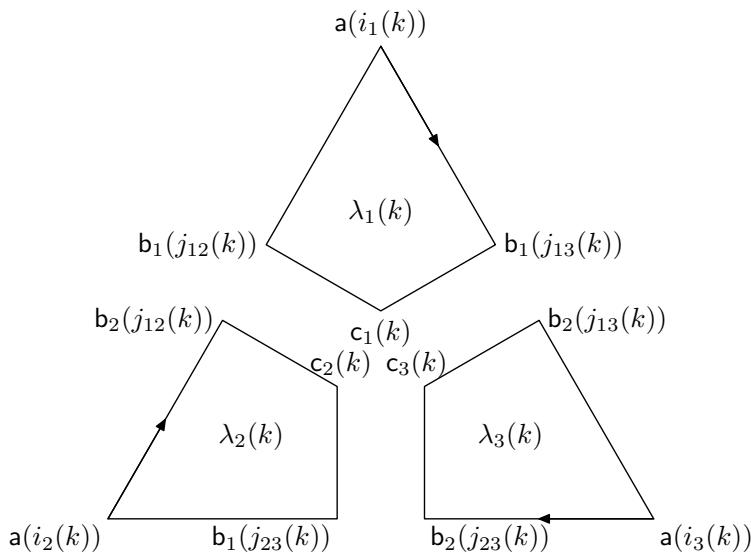
\includegraphics[keepaspectratio]{images/part003_b82e0de6.jpg}}

与 \(f(\mathsf{a}(i_2(j)))\)（在 Y 中）。对 \(i \in \mathsf{I}\)，令 \(d_i \in \mathrm{Grp}(\Gamma)\) 为连接 \(i_0\) 与 \(i\) 的唯一无折返道路（在树 \(\widetilde{\mathsf{T}}\) 中）的类，并令 \(\delta_i = \tau(d_i)\)。

回顾：若 S 是一个集合，则 F(S) 表示 S 上的自由群；在规范映射下元素 \(s \in S\) 在 F(S) 中的像记作 {[}s{]}，在不致混淆时甚至记作 s。

定理 1. --- 假设 Y 道路连通且 f 满足性质 (VK)。沿用前面的记号，存在唯一的群同态

\[
\mathsf {L} \colon \big (\underset {i \in \mathsf {I}} {\ast} \pi_ {1} (\mathrm{X}, \mathsf {a} (i)) \big) \ast \mathrm{F} (\mathrm{J}) \to \pi_ {1} (\mathrm{Y}, f (\mathsf {a} (i _ {0})))
\]

使得

\[
\begin{array}{l l} \mathsf {L} (v) = \delta_ {i} f _ {*} (v) \delta_ {i} ^ {- 1} & \text {for } i\in I \text { and } v\in\pi_{1} (X,a(i)), \\ \mathsf {L} (j) = \delta_ {i _ {1} (j)} \tau (j) \delta_ {i _ {2} (j)} ^ {- 1} & \text {for } j\in J. \end{array}
\]

此外，同态 L 是满射的，其核是包含下列元素的最小正规子群：

\[
\left(\mathrm{R} _ {1}\right) \quad \mathrm{r} _ {1} (j) = j \quad \text {for } j \text { in } \operatorname{Fl} (\mathsf {T});
\]

\[
\left(\mathrm{R} _ {2}\right) \quad \mathfrak {r} _ {2} (j, v) = \varphi_ {j} (v) j \psi_ {j} (v) ^ {- 1} j ^ {- 1} \quad \text {for } j \in \mathsf {J} \text { and } v \in \pi_ {1} (\mathrm{Z}, \mathfrak {b} (j));
\]

\[
\left(\mathrm{R} _ {3}\right) \quad \mathrm{r} _ {3} (k) = \lambda_ {1} (k) j _ {1 2} (k) \lambda_ {2} (k) j _ {2 3} (k) \lambda_ {3} (k) j _ {1 3} (k) ^ {- 1}, \quad \text {for } k \in \mathsf {K}.
\]

同态 L 的存在性与唯一性由自由积与自由群的泛性质得出。此外，这个同态是同态 \(\varpi'(f)_{\gamma(\mathsf{a}(i_0))}\)（由 \(\varpi'(f)\) 通过过渡到迷向群导出）与由 II, 第~208~页命题 5 所定义的群同态 \(\lambda\) 的复合，这里注意到所选取的范坎彭数据确定了群胚态射偶 \((\varpi(p_1), \varpi(p_2))\)（从 \(\varpi(\mathrm{Z})\) 到 \(\varpi(\mathrm{X})\)）的一个完备配备。由该命题，同态 \(\lambda\) 的像是群 \(\operatorname{Coeg}(f)_{\gamma(\mathsf{a}(i_0))}\)，其核是包含由关系 \((\mathrm{R}_1)\)、\((\mathrm{R}_2)\) 与 \((\mathrm{R}_3)\) 所定义的元素的最小正规子群。另一方面，由性质 (VK) 的定义，群胚态射 \(\varpi'(f)\) ： \(\operatorname{Coeg}(f) \to \varpi(\mathrm{Y})\) 是同构。定理于是得证。

\subsection{覆盖}

设 Y 是道路连通、非空的拓扑空间，\((\mathrm{A}_{i})_{i\in\mathrm{I}}\) 是 Y 由非空道路连通子集组成的一个覆盖，以全序集 I 为指标集。令 \(X=\bigsqcup_{i\in I}A_{i}\) 为族 \((\mathrm{A}_{i})\) 的和空间，\(f:X\to Y\) 为由每个 \(A_{i}\) 到 Y 的规范单射组成的族所诱导的映射。假设映射 f 满足性质 (VK)。特别地，这在下列两种情形成立：

\begin{enumerate}
\def\labelenumi{(\roman{enumi})}
\item
  诸集合 \(A_{i}\)（\(i \in I\)）的内部覆盖 Y（参见 IV, 第~402~页，例 2）；
\item
  空间 Y 是可解圈的，诸空间 \(A_{i}\)（\(i \in I\)）亦然，族 \((\mathrm{A}_{i})_{i \in \mathrm{I}}\) 局部有限，诸 \(A_{i}\) 在 Y 中闭，且它们两两的交局部道路连通（参见 IV, 第~399~页，例 1）。
\end{enumerate}

令 J' 为由三元组 \((i, i', V)\) 组成的集合，其中 i 与 \(i'\) 是 I 的元素，V 是 \(A_i \cap A_{i'}\) 的一个道路连通分支。若 \(j = (i, i', V) \in J'\)，则令 \(i_1(j) = i\)，\(i_2(j) = i'\)，并令 \(\overline{j} = (i', i, V)\)。令 J 为 J' 中由满足 \(i < i'\) 的三元组组成的子集。我们称覆盖的框架为这样的箭图 \(\Gamma\)：其顶点集为 I，箭集为 J，源映射与靶映射分别为映射 \(j \mapsto i_1(j)\) 与 \(j \mapsto i_2(j)\)。我们将把与 \(\Gamma\) 相伴的图等同于这样的图 \(\widetilde{\Gamma}\)：其顶点集为 I，箭集为 \(J \cup \overline{J}\)，源映射与靶映射为映射 \(j \mapsto i_{1}(j)\) 与 \(j \mapsto i_{2}(j)\)，其对合为映射 \(j \mapsto \overline{j}\)。

用 \(p_1\) 与 \(p_2\) 表示纤维方块 \(X \times_{Y} X\) 到 X 上的投影；令 \(\textsf{Γ}\) 为群胚态射偶 \((\varpi(p_1), \varpi(p_2))\)（从 \(\varpi(\mathrm{X} \times_{\mathrm{Y}} \mathrm{X})\) 到 \(\varpi(\mathrm{X})\)）的框架。

引理 1. --- 箭图 \(\Gamma\) 可等同于 \(\textsf{Γ}\) 的一个子箭图；箭图 \(\Gamma\) 与 \(\textsf{Γ}\) 都是连通的。

X 的道路连通分支是诸 \(A_{i}\)（\(i \in I\)）。\(X \times_{Y} X\) 的道路连通分支是诸 \((V \times \{i\}) \times_{Y} (V \times \{i'\})\)（\((i, i', V) \in J'\)）。于是，框架 \(\textsf{Γ}\)（属于偶 \((\varpi(p_1), \varpi(p_2))\)）同构于这样的箭图：其顶点集为 I，箭集为 \(J'\)，源映射与靶映射分别为映射 \(j \mapsto i_1(j)\) 与 \(j \mapsto i_2(j)\)。箭图 \(\textsf{Γ}\) 是连通的（IV, 第~406~页）。此外，这一描述把 \(\Gamma\) 等同于 \(\textsf{Γ}\) 的一个子箭图。我们还注意到，对 \(\textsf{Γ}\) 的每条箭 j，或者 \(j \in \mathrm{Fl}(\widetilde{\Gamma})\)，或者存在 \(i \in I\) 使得 \(j = (i, i, A_i)\)。由此推出，映射 \(\pi_0(\Gamma) \to \pi_0(\textsf{Γ})\)（由 \(\Gamma\) 到 \(\textsf{Γ}\) 的单射导出）是双射，从而 \(\textsf{Γ}\) 是连通的。

对 I 的每个元素 \(i\)，选取一点 \(a(i)\)（在 \(\mathrm{A}_i\) 中）。

对每个元素 \(j = (i, i', \mathrm{V})\)（属于 \(\mathrm{J}\)），选取一点 \(b(j)\)（在 \(\mathrm{V}\) 上）、一条道路 \(\mathrm{B}_1(j)\)，它连接 \(b(j)\) 与 \(a(i)\)（在 \(\mathrm{A}_i\) 上），以及一条道路 \(\mathrm{B}_2(j)\)，它连接 \(b(j)\) 与 \(a(i')\)（在 \(\mathrm{A}_{i'}\) 上）。设 \(j = (i, i', \mathrm{V})\) 是 \(\overline{\mathrm{J}}\) 的一个元素；则 \(\overline{j} = (i', i, \mathrm{V})\) 属于 \(\mathrm{J}\)，且令 \(b(\overline{j}) = b(j)\)，\(\mathrm{B}_1(j) = \mathrm{B}_2(\overline{j})\)，\(\mathrm{B}_2(j) = \mathrm{B}_1(\overline{j})\)。对 \(j \in \mathrm{J}' \cup \overline{\mathrm{J}'}\)，道路 \(\overline{\mathrm{B}_1(j)}\) 与 \(\mathrm{B}_2(j)\)（在 \(\mathrm{Y}\) 上）是可拼接的。令

\[
\mathrm{B} (j) = \overline {{\mathrm{B} _ {1} (j)}} * \mathrm{B} _ {2} (j).\tag{3}
\]

这是 Y 中连接 \(a(i_1(j))\) 与 \(a(i_2(j))\) 的一条道路；我们有关系式 \(\mathrm{B}(\overline{j}) = \overline{\mathrm{B}(j)}\)。

对每个 \(j = (i, i', \mathrm{V}) \in \mathrm{J}'\)，用 \(p_{j,1} \colon V \to A_i\) 与 \(p_{j,2} \colon V \to A_{i'}\) 表示规范单射；再用 \(\varphi_j \colon \pi_1(\mathrm{V}, b(j)) \to \pi_1(\mathrm{A}_i, a(i))\) 与 \(\psi_j \colon \pi_1(\mathrm{V}, b(j)) \to \pi_1(\mathrm{A}_{i'}, a(i'))\) 表示由

\[
\varphi_ {j} (v) = [ \mathrm{B} _ {1} (j) ] ^ {- 1} (p _ {j, 1}) _ {*} (v) [ \mathrm{B} _ {1} (j) ]
\]

以及

\[
\psi_ {j} (v) = [ \mathrm{B} _ {2} (j) ] ^ {- 1} (p _ {j, 2}) _ {*} (v) [ \mathrm{B} _ {2} (j) ],
\]

所定义的群同态，其中 \(v \in \pi_1(\mathrm{V}, b(j))\)（参见 IV, 第~407~页）。

固定 I 的一个元素 \(i_0\)，以及箭图 \(\Gamma\) 中的一个子箭图 T，其相伴图 \(\widetilde{T}\) 是图 \(\widetilde{\Gamma}\) 的极大树。

对 \(i \in I\)，设 \((i_0, j_1, i_1, \ldots, j_n, i)\) 是连接 \(i_0\) 与 \(i\) 的唯一无折返道路（在树 \(\widetilde{T}\) 中），并令

\[
\delta (i) = \left[ \mathrm{B} \left(j _ {1}\right) \right] \left[ \mathrm{B} \left(j _ {2}\right) \right] \dots \left[ \mathrm{B} \left(j _ {n}\right) \right];
\]

它是 Y 中连接 \(a(i_0)\) 与 \(a(i)\) 的一条道路的类。用 \(\alpha_i\) 表示由规范单射导出的从 \(\pi_1(\mathrm{A}_i, a(i))\) 到 \(\pi_1(\mathrm{Y}, a(i))\) 的同态，并令 \(\mu_i: \pi_1(\mathrm{A}_i, a(i)) \to \pi_1(\mathrm{Y}, a(i_0))\) 为由下式定义的群同态：

\[
\mu_ {i} (v) = \delta (i) \alpha_ {i} (v) \delta (i) ^ {- 1}.
\]

最后，令 \(\mu\colon\mathrm{F}(\mathrm{J})\to\pi_{1}(\mathrm{Y},a(i_{0}))\) 为唯一的群同态，使得

\[
\mu (j) = \delta (i _ {1} (j)) [ \mathrm{B} (j) ] \delta (i _ {2} (j)) ^ {- 1}
\]

对所有 \(j \in J\) 成立。存在唯一的群同态

\[
\mathsf {M} \colon \big (\underset {i \in \mathrm{I}} {\ast} \pi_ {1} (\mathrm{A} _ {i}, a (i)) \big) \ast \mathrm{F} (\mathrm{J}) \to \pi_ {1} (\mathrm{Y}, a (i _ {0}))
\]

它与 \(\mu_i\) 在每个 \(\pi_1(A_i, a(i))\)（\(i \in I\)）上、与 \(\mu\) 在 \(F(J)\) 上一致。

令 K' 为由四元组 \((i_{1}, i_{2}, i_{3}, \mathrm{U})\) 组成的集合，其中 \(i_{1}, i_{2}, i_{3}\) 是 I 的元素，U 是 \(A_{i_{1}} \cap A_{i_{2}} \cap A_{i_{3}}\) 的一个道路连通分支。对每个元素 \(k = (i_{1}, i_{2}, i_{3}, \mathrm{U})\)（属于 \(K'\)）与每个偶 \((s, t)\)（由 \(\{1, 2, 3\}\) 中的元素组成），令 \(j_{st}(k) = (i_{s}, i_{t}, \mathrm{V})\)，其中 V 是包含 U 的 \(A_{i_{s}} \cap A_{i_{t}}\) 的道路连通分支；这是 \(J'\) 的一个元素。

令 K 为 \(K'\) 中由四元组 \((i_{1}, i_{2}, i_{3}, \mathrm{U})\)（满足 \(i_{1} < i_{2} < i_{3}\)）组成的子集。对 K 的每个元素 \(k = (i_{1}, i_{2}, i_{3}, \mathrm{U})\)，选取 U 的一点 \(c(k)\)，以及道路 \(\mathrm{C}_{12}(k)\)、\(\mathrm{C}_{23}(k)\) 与 \(\mathrm{C}_{13}(k)\)，使得 \(\mathrm{C}_{st}(k)\) 连接 \(c(k)\) 与 \(b(j_{st}(k))\)（在 \(A_{i_{s}} \cap A_{i_{t}}\) 中），这里 \(s, t \in \{1, 2, 3\}\) 满足 s \textless{} t。

然后，对 \(k \in \mathbf{K}\)，令

\[
\mathrm{L} _ {1} (k) = \overline {{\mathrm{B} _ {1} (j _ {1 3} (k))}} * \overline {{\mathrm{C} _ {1 3} (k)}} * \mathrm{C} _ {1 2} (k) * \mathrm{B} _ {1} (j _ {1 2} (k)),\tag{4}
\]

\[
\mathrm{L} _ {2} (k) = \overline {{\mathrm{B} _ {2} (j _ {1 2} (k))}} * \overline {{\mathrm{C} _ {1 2} (k)}} * \mathrm{C} _ {2 3} (k) * \mathrm{B} _ {1} (j _ {2 3} (k)),
\]

\[
\mathrm{L} _ {3} (k) = \overline {{\mathrm{B} _ {2} (j _ {2 3} (k))}} * \overline {{\mathrm{C} _ {2 3} (k)}} * \mathrm{C} _ {1 3} (k) * \mathrm{B} _ {2} (j _ {1 3} (k)).
\]

对 \(s \in \{1,2,3\}\)，用 \(\lambda_s(k)\) 表示 \(\pi_1(\mathrm{A}_{i_s}, a(i_s))\) 中圈 \(\mathrm{L}_s(k)\) 的类。

命题 1. --- 设 Y 是道路连通的拓扑空间，\((\mathrm{A}_{i})_{i\in\mathrm{I}}\) 是 Y 由非空道路连通子集组成、以全序集 I 为指标集的一个覆盖。假设族 \((\mathrm{A}_{i})_{i\in\mathrm{I}}\) 的和空间到 Y 中的规范映射满足性质 (VK)。那么，上面引入的同态 M 是满射的，其核是包含下列元素的最小正规子群：

\[
\begin{array}{l} \text {(R$_ {1}$)} r _ {1} (j) = j \qquad \text {for } j \text { in } \operatorname{Fl}(\mathsf {T}); \\ \text {(R$_ {2}$)} r _ {2} (j, v) = \varphi_ {j} (v) j \psi_ {j} (v) ^ {- 1} j ^ {- 1} \\ \qquad \qquad \qquad \qquad \qquad \qquad \qquad \qquad \qquad \text {for } j = (i,i^{\prime} ,V)\in \mathsf {J} \text { and } v\in\pi_{1} (V,b(j)); \\ \text {(R$_ {3}$)} r _ {3} (k) = \lambda_ {1} (k) j _ {1 2} (k) \lambda_ {2} (k) j _ {2 3} (k) \lambda_ {3} (k) j _ {1 3} (k) ^ {- 1} \\ \qquad \qquad \qquad \qquad \qquad \qquad \qquad \qquad \text {for } k\in \mathsf {K}. \end{array}
\]

设 X 是族 \((\mathrm{A}_{i})_{i\in\mathrm{I}}\) 的和所成的拓扑空间，\(f\colon X\to Y\) 为由每个 \(A_{i}\) 到 Y 的规范单射组成的族所诱导的映射。由假设，映射 f 满足性质 (VK)；因此我们将对它应用第 1 号的定理 1。于是我们沿用该节的记号，并从为映射 f 定义一个范坎彭数据开始。

X 的道路连通分支是诸集合 \(X_{i} = A_{i} \times \{i\}\)（\(i \in I\)）。这样就把 \(\pi_{0}(X)\) 等同于集合 I。对每个 \(i \in I\)，用 \(\mathfrak{a}(i)\) 表示点 \((a(i), i)\)（属于 \(X_{i}\)）。

令 \(Z = X \times_{Y} X\)。\(Z\) 的道路连通分支是诸集合 \(Z_j = (V \times \{i\}) \times_{Y} (V \times \{i'\})\)，其中 \(j = (i, i', V)\) 取遍 \(J'\)。这样就把 \(\pi_0(Z)\) 等同于集合 \(J'\)。令 \(J_0\) 为 \(J\) 中形如 \((i, i, A_i)\) 的元素组成的集合，于是族 \((J_0, J, \overline{J})\) 是 \(J'\) 的一个划分。对 \(i \in I\) 与 \(j = (i, i, A_i) \in J_0\)，令 \(b(j) = (a(i), a(i))\)，并取 \(\beta_1(j)\) 与 \(\beta_2(j)\) 为 \(a(i)\) 处常值道路的类。对 \(j = (i, i', V) \in J \cup \overline{J}\)，用 \(b(j)\) 表示点 \(((b(j), i), (b(j), i'))\)（属于 \(Z_j\)），并用 \(\beta_1(j)\) 与 \(\beta_2(j)\) 表示道路 \(t \mapsto (B_1(j)(t), i)\) 与 \(t \mapsto (B_2(j)(t), i')\)（在 \(X\) 上）的类。

令 \(W = X \times_{Y} X \times_{Y} X\)。W 的道路连通分支是诸集合 \(W_k = (U \times \{i_1\}) \times_{Y} (U \times \{i_2\}) \times_{Y} (U \times \{i_3\})\)，其中 \(k = (i_1, i_2, i_3, U)\) 取遍 \(K'\)。这样就把 \(\pi_0(W)\) 等同于集合 \(K'\)。

用 \(K_{0}\) 表示 \(K'\) 中形如 \(k = (i, i, i, A_{i})\)（\(i \in I\)）的元素组成的集合。对这样的元素 \(k \in K_{0}\)，令 \(\mathsf{c}(k) = (\mathsf{a}(i), \mathsf{a}(i), \mathsf{a}(i))\)，并取 \(\gamma_{st}(k)\) 为 \((\mathsf{a}(i), \mathsf{a}(i))\) 处常值道路的类。

用 \(K_{1}\) 表示 \(K'\) 中形如 \(k = (i_{1}, i_{2}, i_{3}, V)\) 且集合 \(\{i_{1}, i_{2}, i_{3}\}\) 恰有两个元素的元素组成的集合。设 k 是 \(K'\) 中形如 \((i, i, i', V)\) 的元素，使得 \(j = (i, i', V)\) 属于 \(J \cup \overline{J}\)。这时令

\[
\mathsf {c} (k) = ((b (j), i), (b (j), i), (b (j), i ^ {\prime})), \quad \gamma_ {1 2} (k) = (\beta_ {1} (j), \beta_ {1} (j))
\]

并取 \(\gamma_{13}(k)\) 与 \(\gamma_{23}(k)\) 为 \(\mathsf{b}(j)\) 处常值道路的类。类似地定义 \(c(k)\)、\(\gamma_{12}(k)\)、\(\gamma_{13}(k)\)、\(\gamma_{23}(k)\)（对每个元素 \(k\)，属于 \(\mathrm{K}'\)）。

对 K 的每个元素 \(k = (i_{1}, i_{2}, i_{3}, \mathrm{U})\)，令

\[
\mathsf {c} (k) = ((c (k), i _ {1}), (c (k), i _ {2}), (c (k), i _ {3})) ;
\]

对每个偶 \((s,t)\)（由 \(\{1,2,3\}\) 中不同元素组成），取 \(\gamma_{st}(k)\) 为映射 \(x\mapsto((x,s),(x,t))\) 对道路 \(\mathrm{C}_{st}(k)\) 在 \(\mathrm{A}_{i_{s}(k)}\cap\mathrm{A}_{i_{t}(k)}\) 中的类所取的像。

对每个点 \(x = (x_1, x_2, x_3)\)（属于 \(X \times_Y X \times_Y X\)）与每个置换 \(\sigma \in \mathfrak{S}_3\)，令 \(\sigma(x) = (x_{\sigma^{-1}(1)}, x_{\sigma^{-1}(2)}, x_{\sigma^{-1}(3)})\)。这样就定义了群 \(\mathfrak{S}_3\) 在 W 上的一个作用。对每个 \(k = (i_1, i_2, i_3, U) \in K'\) 与每个置换 \(\sigma \in \mathfrak{S}_3\)，类似地令 \(\sigma(k) = (i_{\sigma^{-1}(1)}, i_{\sigma^{-1}(2)}, i_{\sigma^{-1}(3)}, U)\)；我们有

\[
\sigma \left(\mathrm{W} _ {k}\right) = \left(\mathrm{U} \times \left\{i _ {\sigma^ {- 1} (1)} \right\}\right) \times_ {\mathrm{Y}} \left(\mathrm{U} \times \left\{i _ {\sigma^ {- 1} (2)} \right\}\right) \times_ {\mathrm{Y}} \left(\mathrm{U} \times \left\{i _ {\sigma^ {- 1} (3)} \right\}\right) = \mathrm{W} _ {\sigma (k)}.
\]

设 \(k = (i_1, i_2, i_3, \mathrm{U})\) 是 \(\mathrm{K}'\) 的元素，且 \(i_1, i_2, i_3\) 两两不同。存在唯一的置换 \(\sigma \in \mathfrak{S}_3\) 使得 \(i_{\sigma^{-1}(1)} < i_{\sigma^{-1}(2)} < i_{\sigma^{-1}(3)}\)，亦即使得 \(\sigma(k) = (i_{\sigma^{-1}(1)}, i_{\sigma^{-1}(2)}, i_{\sigma^{-1}(3)}, \mathrm{U})\) 属于 \(\mathrm{K}\)。对 \(s \in \{1, 2, 3\}\)，令 \(c_s(k) = c_{\sigma(s)}(\sigma(k))\)，\(c(k) = (c_1(k), c_2(k), c_3(k))\)，于是 \(c(k) = \sigma^{-1}(c(\sigma(k)))\)。对 \((s, t) \in \{(1, 2), (1, 3), (2, 3)\}\)，定义 \(\mathrm{C}_{st}(k) = \mathrm{C}_{\sigma^{-1}(s)\sigma^{-1}(t)}(\sigma(k))\)；这是连接 \(c(k)\) 与 \(b(j_{\sigma(s)\sigma(t)}(\sigma(k))) = b(j_{st}(k))\) 的一条道路。

用 \(g\) 表示从 \(\Gamma\) 到 \(\textsf{Γ}\) 的箭图态射，它把顶点 \(i \in I\)（属于 \(\Gamma\)）对应为顶点 \(X_i = A_i \times \{i\}\)（属于 \(\textsf{Γ}\)），把箭 \(j = (i, i', V) \in J'\)（属于 \(\Gamma\)）对应为箭 \(Z_j = (V \times \{i\}) \times_Y(V \times \{i'\})\)（属于 \(\textsf{Γ}\)）。映射 Som( \(g\) ) 是双射；映射 Fl( \(g\) ) 是单射，且图 \(\Gamma\) 连通（IV, 第~410~页，引理 1），并且子箭图 T 在 \(g\) 下的像是一个子箭图 \(\mathsf{T}\)（属于 \(\textsf{Γ}\)），其相伴图是图 \(\widetilde{\textsf{Γ}}\) 的极大树。

诸点 \(\mathsf{a}(i)\)（\(i \in I\)）、点 \(\mathsf{b}(j)\)（\(j \in J'\)）、诸点 \(\mathsf{c}(k)\)（\(k \in K'\)）、道路类 \(\beta_{1}(j)\) 与 \(\beta_{2}(j)\)（\(j \in J'\)）、道路类 \(\gamma_{st}(k)\)（\(k \in \mathrm{K}'\)）、子箭图 \(g(\mathrm{T})\)（属于 \(\textsf{Γ}\)）以及元素 \(i_0\)（属于 I）定义了 \(f\) 的一个范坎彭数据。

用 \(\rho\) 表示唯一的群同态

\[
\rho \colon \big (\underset {i \in \mathrm{I}} {*} \pi_ {1} (\mathrm{X}, \mathsf {a} (i)) \big) * \mathrm{F} (\mathrm{J} ^ {\prime}) \to \big (\underset {i \in \mathrm{I}} {*} \pi_ {1} (\mathrm{A} _ {i}, a (i)) \big) * \mathrm{F} (\mathrm{J})
\]

它在 \(\pi_1(\mathrm{X},\mathsf{a}(i))\) 与 \(\pi_1(\mathrm{A}_i,a(i))\) 之间诱导出由 \(\mathrm{A}_i\times \{i\}\) 与 \(\mathrm{A}_i\) 的等同所导出的同构（对每个 \(i\in \mathrm{I}\)），并且使得

\[
\begin{array}{l l} \rho (j) = 1 & \text {for } j \in \mathrm{J} _ {0} \\ \rho (j) = j, \quad \rho (\overline {{j}}) = j ^ {- 1} & \text {for } j \in \mathrm{J}. \end{array}
\]

设 L 为 IV, 第~408~页定理 1 中所定义的群同态。对 \(j = (i, i, \mathrm{A}_i) \in \mathrm{J}_0\)，我们有 \(\mathsf{L}(j) = 1 = \mathsf{M} \circ \rho(j)\)。设 \(j = (i, i', \mathrm{V})\) 是 J 的一个元素；由定义我们有 \(\mathsf{L}(j) = (\mathsf{M} \circ \rho)(j)\)。最后，若 \(j = (i, i', \mathrm{V})\) 是 \(\overline{\mathbf{J}}\) 的一个元素，则 \(\overline{j} \in \mathbf{J}\)，并且可以验证

\[
\mathsf {L} (j) = \mathsf {L} (\overline {{j}}) ^ {- 1} = \mathsf {M} (\rho (\overline {{j}})) ^ {- 1} = \mathsf {M} (\rho (j)).
\]

于是，我们有 M ∘ ρ = L。

同态 L 是满射的（出处同上），因此同态 M 也是满射的。由于同态 \(\rho\) 是满射的，M 的核是 \(\left(\ast\pi_{1}(\mathrm{A}_{i},a(i))\right)*\mathrm{F}(\mathrm{J})\) 中包含在 \(\rho\) 下定理 1（IV, 第~408~页）的关系 \((\mathrm{R}_{1})\)、\((\mathrm{R}_{2})\)、\((\mathrm{R}_{3})\) 所定义元素的像的最小正规子群。只需验证这些像，除了命题 1 的关系 \((\mathrm{R}_{1})\)、\((\mathrm{R}_{2})\)、\((\mathrm{R}_{3})\) 所定义的元素之外，还包括与它们共轭的元素、或与其逆共轭的元素，以及单位元，证明即告完成。

元素 R \(_{1}\) --- 定向树 T 的一条箭形如 Z \(_{j}\)，其中 \(j = (i, i', V) \in J\)；它的像是 F(J) 的元素 \(j\)。

元素 R₂. --- 设 \(j = (i, i', \mathrm{V}) \in \mathrm{J}'\)。若 \(i = i'\)，我们有 \(\rho(\mathsf{r}_2(j, v)) = 1\)（对所有 \(v \in \pi_1(\mathrm{A}_i, \mathsf{a}(i))\)）。若 \(j \in J\)，则 \(\mathsf{r}_2(j, v)\) 的像是元素 \(r_2(j, v) = \varphi_j(v) j \psi_j(v)^{-1} j^{-1}\)（对每个 \(v \in \pi_1(\mathrm{Z}, \mathsf{b}(j))\)）。在余下的情形，我们有 \(\overline{j} \in J\)，且等式

\[
\begin{array}{r l} & {\rho (\mathtt {r} _ {2} (j, v)) = \rho (\varphi_ {j} (v) j \psi_ {j} (v) ^ {- 1} j ^ {- 1})} \\ & {\qquad = [ \mathrm{B} _ {1} (j) ] ^ {- 1} v [ \mathrm{B} _ {1} (j) ] \rho (j) [ \mathrm{B} _ {2} (j) ] ^ {- 1} v ^ {- 1} [ \mathrm{B} _ {2} (j) ] \rho (j) ^ {- 1}} \\ & {\qquad = [ \mathrm{B} _ {2} (\bar {j}) ] ^ {- 1} v [ \mathrm{B} _ {2} (\bar {j}) ] \bar {j} ^ {- 1} [ \mathrm{B} _ {1} (\bar {j}) ] ^ {- 1} v ^ {- 1} [ \mathrm{B} _ {1} (\bar {j}) ] \bar {j}} \end{array}
\]

表明 \(\rho(\mathsf{r}_2(j,v))\) 与 \(\rho(\mathsf{r}_2(\overline{j},v^{-1}))\) 共轭。

元素 R₃. — 设 \(k = (i_{1}, i_{2}, i_{3}, \mathrm{U})\) 是 K' 的一个元素。

若 \(k \in \mathrm{K}_0\)，则 \(i_1 = i_2 = i_3\)，\(\lambda_s(k)\) 对所有 \(s \in \{1,2,3\}\) 是平凡道路的类，且 \(j_{st}(k) \in \mathrm{J}_0\) 对每个偶 \((s,t) \in \{(1,2),(1,3),(2,3)\}\) 成立。此时 \(\rho(\mathsf{r}_3(k))\) 是单位元。

设 \(k\in \mathrm{K}_1\)。若 \(i_1 = i_2\)，则 \(j = (i_{1},i_{3},\mathrm{U})\in \mathrm{J}\cup \overline{\mathrm{J}}\)，并且有

\[
\mathsf {r} _ {3} (k) = \beta_ {1} (j) ^ {- 1} j _ {1 2} \beta_ {1} (j) j _ {2 3} \beta_ {2} (j) ^ {- 1} \beta_ {2} (j) j _ {1 3} ^ {- 1}
\]

它在 \(\rho\) 下的像是单位元。其余情形类似处理。

设 \(i_{1}, i_{2}, i_{3}\) 两两不同。若 \(i_{1} < i_{2} < i_{3}\)，则 \(k \in \mathbf{K}\)，且 \(\rho(\mathsf{r}_{3}(k))\) 的像是元素 \(r_{3}(k)\)。

设 \(\sigma \in \mathfrak{S}_3\) 为把 1 映到 2、把 2 映到 3 的置换。我们有

\[
\begin{array}{r l} \lambda_ {1} (\sigma (k)) & = \beta_ {1} (j _ {1 3} (\sigma (k))) ^ {- 1} \cdot p _ {1, *} (\gamma_ {1 3} (\sigma (k))) ^ {- 1} \cdot \\ & \qquad \cdot p _ {1, *} (\gamma_ {1 2} (\sigma (k))) \cdot \beta_ {1} (j _ {1 2} (\sigma (k))) \\ & = \beta_ {1} (j _ {3 2} (k)) ^ {- 1} \cdot p _ {1, *} (\gamma_ {3 2} (k)) ^ {- 1} \cdot p _ {1, *} (\gamma_ {3 1} (k)) \cdot \beta_ {1} (j _ {3 1} (k)) \\ & = \beta_ {2} (j _ {2 3} (k)) ^ {- 1} \cdot p _ {2, *} (\gamma_ {2, 3} (k)) ^ {- 1} \cdot p _ {2, *} (\gamma_ {1 3} (k)) \cdot \beta_ {2} (j _ {1 3} (k)) \\ & = \lambda_ {3} (k). \end{array}
\]

我们类似地验证 \(\lambda_2(\sigma(k)) = \lambda_1(k)\) 与 \(\lambda_3(\sigma(k)) = \lambda_2(k)\)。于是，

\[
\begin{array}{r l} & {\rho (\mathsf {r} _ {3} (\sigma (k))) = \lambda_ {1} (\sigma (k)) \rho (j _ {1 2} (\sigma (k))) \lambda_ {2} (\sigma (k)) \cdot} \\ & {\qquad \cdot \rho (j _ {2 3} (\sigma (k))) \lambda_ {3} (\sigma (k)) \rho (j _ {1 3} (\sigma (k))) ^ {- 1}} \\ & {\qquad = \lambda_ {3} (k) \rho (j _ {3 1} (k)) \lambda_ {1} (k) \rho (j _ {1 2} (k)) \lambda_ {2} (k) \rho (j _ {3 2} (k)) ^ {- 1}} \\ & {\qquad = \lambda_ {3} (k) j _ {1 3} (k) ^ {- 1} \lambda_ {1} (k) j _ {1 2} (k) \lambda_ {2} (k) j _ {2 3} (k),} \end{array}
\]

这证明 \(\rho(\mathsf{r}_3(\sigma(k)))\) 共轭于

\[
\lambda_ {1} (k) j _ {1 2} (k) \lambda_ {2} (k) j _ {2 3} (k) \lambda_ {3} (k) j _ {1 3} (k) ^ {- 1} = \rho (\mathsf {r} _ {3} (k)).
\]

设 \(\tau \in \mathfrak{S}_3\) 为支集为 \(\{1,2\}\) 的对换。我们有

\[
\lambda_ {1} (\tau (k)) = \lambda_ {2} (k) ^ {- 1}, \quad \lambda_ {2} (\tau (k)) = \lambda_ {1} (k) ^ {- 1} \quad \text {and} \quad \lambda_ {3} (\tau (k)) = \lambda_ {3} (k) ^ {- 1}.
\]

等式

\[
\begin{array}{c} \rho (\mathsf {r} _ {3} (\tau (k))) = \lambda_ {2} (k) ^ {- 1} \rho (j _ {2 1} (k)) \lambda_ {1} (k) ^ {- 1} \rho (j _ {1 3} (k)) \lambda_ {3} (k) ^ {- 1} \rho (j _ {2 3} (k)) ^ {- 1} \\ = \big (\rho (j _ {2 3} (k)) \lambda_ {3} (k) \rho (j _ {1 3} (k)) ^ {- 1} \lambda_ {1} (k) \rho (j _ {1 2} (k)) \lambda_ {2} (k) \big) ^ {- 1} \end{array}
\]

表明 \(\rho(\mathsf{r}_3(\tau(k)))\) 共轭于

\[
\lambda_ {1} (k) \rho (j _ {1 2} (k)) ^ {- 1} \lambda_ {2} (k) \rho (j _ {2 3} (k)) \lambda_ {3} (k) \rho (j _ {1 3} (k)) ^ {- 1} = \rho (\mathsf {r} _ {3} (k)).
\]

由于群 \(\mathfrak{S}_3\) 由置换 \(\tau\) 与 \(\sigma\) 生成，由此推出，对每个 \(k \in \mathrm{K}\) 与每个 \(\sigma \in \mathfrak{S}_3\)，\(\rho(\mathsf{r}_3(\sigma(k)))\) 共轭于 \(\rho(\mathsf{r}_3(k))\) 或其逆。

命题 1 于是得证。

推论 1. --- 在命题 1 的假设之下，再设对每个 \(i \in I\)，从 \(\pi_1(A_i, a(i))\) 到 \(\pi_1(Y, a(i))\) 的同态（由 \(A_i\) 到 Y 的规范单射导出）的像是平凡的。于是由 M 经限制得到的同态 \(M': F(J) \to \pi_1(Y, a(i_0))\) 是满射的，其核是包含元素 \(j \in Fl(T)\) 以及元素 \(j_{12}(k) j_{23}(k) j_{13}(k)^{-1}\)（\(k \in K\)）的最小正规子群。

设 \(\pi\colon (*_{i\in\mathrm{I}}\pi_1(\mathrm{A}_i,a(i)))*\mathrm{F}(\mathrm{J})\to\mathrm{F}(\mathrm{J})\) 为在每个 \(\pi_1(\mathrm{A}_i,a(i))\) 上诱导平凡同态、在 \(\mathrm{F}(\mathrm{J})\) 上诱导恒等同态的唯一同态；它是满射的。设 \(i\in\mathrm{I}\)。由 \(\mathsf{M}\) 的定义以及由规范单射导出的、从 \(\pi_1(\mathrm{A}_i,a(i))\) 到 \(\pi_1(\mathrm{Y},a(i))\) 的同态之像平凡这一假设，可以推出：对每个 \(v\in\pi_1(\mathrm{A}_i,a(i))\)，\(\mathsf{M}(v)\) 是 \(\pi_1(\mathrm{Y},a(i_0))\) 的单位元。因此我们有 \(\mathsf{M}=\mathsf{M}'\circ\pi\)。于是同态 \(\mathsf{M}'\) 是满射的，其核是包含在 \(\pi\) 下命题 1 中所定义的元素 \(r_1(j)\)、\(r_2(j,v)\) 与 \(r_3(k)\) 的像的最小正规子群。对 \(j\in\mathrm{Fl}(\mathrm{T})\)，我们有 \(\pi(r_1(j))=j\)。对所有 \(j\in\mathrm{J}\) 与每个 \(v\in\pi_1(\mathrm{V},b(j))\)，我们有 \(\pi(r_2(j,v))=e\)。最后，对每个 \(k=(i_1,i_2,i_3,\mathrm{U})\in\mathrm{K}\) 与每个 \(s\in\{1,2,3\}\)，\(\lambda_s(k)\) 是 \(\mathrm{A}_{i_s}\) 中一个圈的类；因此 \(\pi(\lambda_s(k))=e\)，从而 \(\pi(r_3(k))=j_{12}(k)j_{23}(k)j_{13}(k)^{-1}\)。推论由此得出。

推论 2. --- 在命题 1 的假设之下，再设对每个 \(i \in I\)，群 \(\pi_1(A_i, a(i))\) 都化为单位元，并且对 I 中两两不同元素的每个三元组 \((i_1, i_2, i_3)\)，集合 \(A_{i_1} \cap A_{i_2} \cap A_{i_3}\) 都是空集。于是同态 \(\mathsf{M}''\colon \mathrm{F}(\mathrm{J} - \mathrm{Fl}(\mathrm{T})) \to \pi_1(\mathrm{Y}, a(i_0))\)（由 \(\mathsf{M}\) 经限制得到）是同构。

设 \(\pi'\colon\mathrm{F}(\mathrm{J})\to\mathrm{F}(\mathrm{J}-\mathrm{Fl}(\mathrm{T}))\) 为这样的同态：它把 \([j]\) 映到 \([j]\)（当 \(j\in\mathrm{J}-\mathrm{Fl}(\mathrm{T})\)），把 \([j]\) 映到单位元（当 \(j\in\mathrm{Fl}(\mathrm{T})\)）；它是满射的，并且我们有 \(\mathsf{M}''\circ\pi'= \mathsf{M}'\)，其中 \(\mathsf{M}'\) 是推论 1 中定义的满射同态。由此推出 \(\mathsf{M}''\) 是满射的，其核是 \(\mathrm{F}(\mathrm{J}-\mathrm{Fl}(\mathrm{T}))\) 中包含在 \(\pi'\) 下出处所述元素的像的最小正规子群。而按构造，\(\pi'(j) = e\)（若 \(j \in \mathrm{Fl}(T)\)），且由假设集合 K 是空集。因此同态 \(M''\) 是同构。

例. --- 1) 关于由两个集合组成的覆盖的情形，见第 3 号。

\begin{enumerate}
\def\labelenumi{\arabic{enumi})}
\setcounter{enumi}{1}
\tightlist
\item
  设 G 是一个图（II, 第~155~页，定义 1）；用 S 表示 G 的顶点集，A 表示其定向边集，o 与 t 表示从 A 到 S 的起点映射与终点映射；对每条定向边 \(a \in A\)，用 \(\overline{a}\) 表示相反的定向边。给集合 S 与 A 赋以离散拓扑；令 X 为空间 S 与空间 I × A 的和空间，并令 ∼ 为 X 上使得 \((u, a) \sim (1 - u, \overline{a})\)、\((0, a) \sim o(a)\) 与 \((1, a) \sim t(a)\)（对所有 \(u \in I\) 与每条定向边 \(a \in A\)）的最细等价关系。商空间 \(|G| = X / \sim\) 称为图 G 的几何实现。我们用 p 表示 X 到 \(|G|\) 上的规范投影。
\end{enumerate}

我们来证明 \(|\mathbf{G}|\) 是局部可缩的。设 \(s \in S\)。用 \(\mathrm{X}_s\) 表示 \(\{s\}\) 与诸子集 \([0,1[ \times \{a\}\)（\(a \in o^{-1}(s)\)）以及诸子集 \(]0,1] \times \{a\}\)（\(a \in t^{-1}(s)\)）的并。令 \(\mathrm{U}_s\) 为 \(\mathrm{X}_s\) 在 \(|\mathbf{G}|\) 中的像；它是 \(p(s)\) 在 \(|\mathbf{G}|\) 中的开邻域，因为 \(\mathrm{X}_s\) 是 \(s\) 在 \(X\) 中的饱和开邻域。令 \(f\) 为从 \(\mathrm{X}_s \times \mathbf{I}\) 到 \(\mathrm{X}_s\) 中的、由下列关系式（对 \(u, v \in \mathbf{I}\) 与 \(a \in A\)）定义的映射

\[
\begin{array}{c} f (s, v) = s \\ f ((u, a), v) = \left\{ \begin{array}{l l} ((1 - v) u, a) & \text {if } 0 \leqslant u <   1 \text {and } o (a) = s, \\ (1 - (1 - v) (1 - u), a) & \text {if } 0 <   u \leqslant 1 \text {and } t (a) = s. \end{array} \right. \end{array}
\]

它是连续的且与等价关系 ∼ 相容。因此，通过过渡到商，它定义了一个映射 \(\varphi_{s}\colon U_{s}\times I\to U_{s}\)，由于 I 局部紧（I, 第~19~页，命题 10），该映射是连续的。它是 \(U_{s}\) 到 \(p(s)\) 上的一个强收缩（III, 第~237~页，定义 6）。

此外设 \(x = (\tau, a) \in ]0, 1[ \times \mathrm{A}\)。令 \(\mathrm{X}_x = ]0, 1[ \times \{a, \overline{a}\}\)，并令 \(\mathrm{U}_x\) 为它在 \(|\mathbf{G}|\) 中（在 \(p\) 之下）的像；它是 \(p(x)\) 在 \(|\mathbf{G}|\) 中的邻域，同胚于 \(]0, 1[\)。从 \(\mathrm{X}_x \times \mathbf{I}\) 到 \(\mathrm{X}_x\) 中的、由 \(((u, a), v) \mapsto ((1 - v)u + v\tau, a)\) 与 \(((u, \overline{a}), t) \mapsto ((1 - v)u + v(1 - \tau), \overline{a})\) 给出的映射是连续的。通过过渡到商，它定义了一个映射 \(\varphi_x: \mathrm{U}_x \times \mathbf{I} \to \mathrm{U}_x\)，它是连续的（出处同上），且是到 \(x\) 处的一个强收缩。

\(|\mathbf{G}|\) 的每个点都是某个点 \(s \in \mathbf{S}\) 的像，或者是 \(\mathbf{I} \times \mathbf{A}\) 中形如 \((\tau, a)\)（其中 \(0 < \tau < 1\)）的点的像。由此推出，\(|\mathbf{G}|\) 的每个点都有在该点处可缩的邻域。换言之，\(|\mathbf{G}|\) 是局部可缩的，特别地是单连通的（IV, 第~346~页，命题 5）。

在 S 上选取一个全序，并考虑由 \((\mathrm{U}_{s})_{s\in\mathrm{S}}\) 组成的 \(|G|\) 的开覆盖。设 s 与 \(s'\) 是 S 的不同元素。交 \(U_{s}\cap U_{s'}\) 是诸 \(p([0,1[,a)\) 的并，其中 a 取遍 G 的以 s 与 \(s'\) 为端点的定向边的集合。于是，覆盖 \((\mathrm{U}_{s})_{s\in\mathrm{S}}\) 的神经等同于箭图 G。此外，对每个 \(s\in S\)，\(U_{s}\) 在 s 处可缩，因此 \(\pi_{1}(\mathrm{U}_{s},p(s))\) 化为单位元。于是由 IV, 第~416~页的推论 2 得出，对每个 \(s\in S\)，\(\pi_{1}(|\mathrm{G}|,p(s))\) 是自由群（尼尔森–施赖尔定理）。

推论 3. --- 在命题 1 的假设之下，再设覆盖 (A \(_{i}\) ) \(_{i\in I}\) 的框架是一个定向树。于是由 M 经限制得到的同态 N: * \(_{i\in I} \pi_{1}(A_{i},a(i)) \to \pi_{1}(Y,a(i_{0}))\) 是满射的；其核是 * \(_{i\in I} \pi_{1}(A_{i},a(i))\) 中包含元素 \(\varphi_{j}(v)\psi_{j}(v)^{-1}\)（对每个 \(j = (i_{1},i_{2},V) \in J\) 与每个 \(v \in \pi_{1}(V,b(j))\)）的最小正规子群。

如果此外诸交 \(A_{i} \cap A_{i'}\)（\(i \neq i'\)）的道路连通分支还是道路单连通的，那么同态 N 是同构。

在该推论的假设之下，与箭图 \(\Gamma\) 相伴的图是一棵树，从而 \(T = \Gamma\)。由此推出，群 \(F(J)\) 在同态 \(M\) 下的像化为单位元。

设

\[
\rho \colon \big (\underset {i \in \mathrm{I}} {\ast} \pi_ {1} (\mathrm{A} _ {i}, a (i)) \big) \ast \mathrm{F} (\mathrm{J}) \to \underset {i \in \mathrm{I}} {\ast} \pi_ {1} (\mathrm{A} _ {i}, a (i))
\]

为在 \(\pi_1(A_i, a(i))\) 上诱导恒等同态且其核包含 F(J) 的唯一群同态。我们有 M = N \(\circ\) \(\rho\)。于是同态 N 是满射的，其核是 \(*_{i \in I} \pi_1(A_i, a(i))\) 中包含在 \(\rho\) 下命题 1 的关系 (R \(_1\) )、(R \(_2\) ) 与 (R \(_3\) ) 所定义元素的像的最小正规子群。我们有 \(\rho(j) = 1\)（对所有 \(j \in \text{Fl}(\Gamma)\)）。由于覆盖 (A \(_i\) ) \(_{i \in I}\) 的框架是一棵树，有 A \(_{i_1} \cap\) A \(_{i_2} \cap\) A \(_{i_3} = \varnothing\)（对 I 中不同元素的每个三元组 \(i_1, i_2, i_3\) ）。由此推出，N 的核是包含元素 \(\varphi_j(v) \psi_j(v)^{-1}\)（对所有 \(j = (i_1, i_2, V) \in J\) 与每个 \(v \in \pi_1(V, b(j))\)）的最小正规子群。

例 3（去掉 n 个点的平面）。--- \(R^{2}-\{0\}\) 的基本群同构于 Z，且道路 \(t \mapsto e^{2\pi it}\) 的类是它的一个生成元（IV, 第~347~页，推论）。更一般地，设 n 是自然数，\(A = \{z_{1}, \ldots, z_{n}\}\) 是 \(R^{2}\) 的由 n 个点组成的集合。令 Y 为空间 \(R^{2}-A\)；我们将证明 Y 的基本群同构于 n 个生成元上的自由群 \(F_{n}\)。对每个 i，令 \(z_{i} = (u_{i}, v_{i})\)。在必要时把 \(z_{i}\) 换成 \(f(z_{i})\)（其中 \(f: R^{2} \to R^{2}\) 是形如 \((u, v) \mapsto (u + \alpha v, v)\) 的同胚）之后，可以假设诸 \(z_{i}\) 的横坐标两两不同。假设 \(u_{1} < \cdots < u_{n}\) 也不失一般性。

令 \(V_{1} = ]-\infty, u_{2}[ \times R\)，\(V_{i} = ]u_{i-1}, u_{i+1}[ \times R\)（对 \(2 \leqslant i \leqslant n-1\)），\(V_{n} = ]u_{n-1}, +\infty[ \times R\)。对 \(1 \leqslant i \leqslant n\)，集合 \(U_{i} = V_{i} - \{z_{i}\}\) 在平面中是开集且同胚于 \(R^{2} - \{0\}\)。族 \((U_{i})_{1 \leqslant i \leqslant n}\) 是空间 \(Y = R^{2} - A\) 的一个开覆盖。交 \(U_{i} \cap U_{j}\) 在 \(|i - j| \geqslant 2\) 时是空集，同胚于 \(R^{2}\)（当 \(|i - j| = 1\)）。由推论 3，Y 的基本群同构于自由群 \(F_{n}\)。

设 \(a\) 是 Y 的一点。对每个整数 \(i \in \{1, \ldots, n\}\)，取一严格正实数 \(r_i\)，它严格小于 \(z_i\) 到诸点 \(z_j\)（\(j \neq i\)）的距离。用 \(v_i\) 表示圈 \(t \mapsto z_i + r_i e^{2\pi it}\) 在 Y 的点 \(z_i + r_i\) 处的类。令 \(\theta_i\) 为一条道路 \(\gamma_i\)（它连接点 \(a\) 与点 \(z_i + r_i\)）在 Y 中的类。如果诸道路 \(\gamma_i\) 都是单射的且它们的像仅在 \(a\) 处相交，那么可以证明，从自由群 F( \(t_1, \ldots, t_n\) ) 到 \(\pi_1(Y, a)\)、使得 \(\varphi(t_i) = \theta_i v_i \theta_i^{-1}\)（对所有 \(i \in \{1, \ldots, n\}\)）的唯一同态是群同构。

类似的论证可以证明：对平面的任意闭离散子集 A，\(R^{2}-A\) 的基本群同构于 F(A)（IV, 第~463~页，习题 1）。

推论 4. --- 在命题 1 的假设之下，设存在 Y 的一个非空道路连通子集 A，使得交 \(\mathrm{A}_i \cap \mathrm{A}_{i'}\) 对每个偶 \((i, i')\)（由 I 中不同元素组成）都等于 A。设 a 是 A 的一点。存在唯一的同态 \(\varphi\)，从群族 \((\pi_1(\mathrm{A}_i, a))_{i \in \mathrm{I}}\) 被 \(\pi_1(\mathrm{A}, a)\) 黏合的和到 \(\pi_1(\mathrm{Y}, a)\) 上，它与由 \(\mathrm{A}_i\) 到 Y 的规范单射导出的同态一致（对每个 \(i \in \mathrm{I}\)）。同态 \(\varphi\) 是同构。

特别地，若群 \(\pi_{1}(\mathrm{A},a)\) 化为单位元，则群族 \((\pi_1(\mathrm{A}_i,a))_{i\in \mathrm{I}}\) 的自由积到 \(\pi_1(\mathrm{Y},a)\) 上的规范同态是同构。

对 \(i \in \mathrm{I}\)，用 \(g_i \colon \pi_1(\mathrm{A}, a) \to \pi_1(\mathrm{A}_i, a)\) 与 \(f_i \colon \pi_1(\mathrm{A}_i, a) \to \pi_1(\mathrm{Y}, a)\) 表示由 \(\mathrm{A}\) 到 \(\mathrm{A}_i\) 以及 \(\mathrm{A}_i\) 到 \(\mathrm{Y}\) 的包含关系导出的规范同态。用 \(*_{\mathrm{A}} \pi_1(\mathrm{A}_i, a)\) 表示诸群 \(\pi_1(\mathrm{A}_i, a)\) 被 \(\pi_1(\mathrm{A}, a)\) 黏合的和。再令 \(p\) 为从 \(*_{i \in \mathrm{I}} \pi_1(\mathrm{A}_i, a)\) 到 \(*_{\mathrm{A}} \pi_1(\mathrm{A}_i, a)\) 上、在 \(\pi_1(\mathrm{A}_i, a)\) 上诱导恒等同态的唯一同态（A, I, 第~80~页，命题 4）。同态 \(p\) 是满射的，并且由幺半群 \(*_{\mathrm{A}} \pi_1(\mathrm{A}_i, a)\) 的定义可知，其核是 \(*_{i \in \mathrm{I}} \pi_1(\mathrm{A}_i, a)\) 中包含元素 \(g_i(v)g_{i'}(v)^{-1}\)（对 \(i, i' \in \mathrm{I}\) 与 \(v \in \pi_1(\mathrm{A}, a)\)）的最小正规子群。

诸同态 \(f_i \circ g_i \colon \pi_1(A, a) \to \pi_1(Y, a)\)（\(i \in I\)）相等。于是由幺半群黏合和的泛性质（A, I, 第~80~页，命题 4），存在唯一的群同态 \(\varphi\)（相应地 \(f\)），从 \(*_{A} \pi_1(A_i, a)\)（相应地从 \(*_{i \in I} \pi_1(A_i, a)\)）到 \(\pi_1(Y, a)\) 中，它诱导出同态 \(f_i\)（到 \(\pi_1(A_i, a)\) 上）。我们有 \(f = \varphi \circ p\)。

对 \(i \in I\)，用 \(u_i\) 表示 A 到 \(A_i\) 中的规范单射，\(v_i\) 表示 \(A_i\) 到 Y 中的规范单射。再用 \(w\) 表示 A 到 Y 中的规范单射。对每个 \(i \in I\)，我们有 \(v_i \circ u_i = w\)，因此 \(\pi_1(v_i, a) \circ \pi_1(u_i, a) = \pi_1(w, a)\)。于是由幺半群黏合和的泛性质（A, I, 第~80~页，命题 4），存在唯一的群同态 \(\varphi\)，从 \(*_{i} \pi_1(A_i, a)\) 到 \(\pi_1(Y, a)\) 上，它诱导出同态 \(\pi_1(v_i, a)\)（到 \(\pi_1(A_i, a)\) 上）。需要证明的是 \(\varphi\) 是同构。

集合 J 等同于由元素偶 \((i, i')\)（属于 I）组成的、满足 \(i < i'\) 的集合。集合 K 等同于由元素三元组 \((i_{1}, i_{2}, i_{3})\)（属于 I）组成的、满足 \(i_{1} < i_{2} < i_{3}\) 的集合。我们选取所有基点 \(a(i)\)、\(b(j)\) 与 \(c(k)\) 都等于 a，所有道路 \(\mathrm{B}(j)\) 与 \(\mathrm{C}_{st}(k)\) 都等于以 a 为像的常值道路。我们再固定一点 \(i_{0} \in I\)。

对每个偶 \((i, i')\)（由 I 的不同点组成），框架 \(\Gamma\)（覆盖 \((\mathrm{A}_{i})\) 的）恰有一条以 i 与 \(i'\) 为端点的箭。\(\Gamma\) 的有一条端点等于 \(i_{0}\) 的箭构成一棵极大定向树 T 的箭。

对每个元素 \(k \in \mathrm{K}\)，我们有 \(r_3(k) = j_{12}(k)j_{23}(k)j_{13}(k)^{-1}\)；令 R 为 \(\mathrm{F(J)}\) 的由元素 \(j \in \mathrm{Fl(T)}\) 与元素 \(r_3(k)\)（\(k \in \mathrm{K}\)）生成的正规子群。我们来证明 \(\mathrm{R} = \mathrm{F(J)}\)。只需证明 J 的每个元素 \(j = (i_1, i_2)\) 都属于 R。由假设，当 \(i_1 = i_0\) 或 \(i_2 = i_0\) 时这是真的。设 \(i_0 < i_1\)，并令 \(k = (i_0, i_1, i_2)\)。它是 K 的元素，且 \(j = j_{23}(k) = j\)。此外，\(j_{12}(k)\) 与 \(j_{13}(k)\) 属于 Fl(T)。由此推出 \(j\) 属于 R。\(i_1 < i_0 < i_2\) 或 \(i_2 < i_0\) 的情形类似处理。

于是由命题 1（IV, 第~412~页）得出，同态 \(f\) 是满射的，其核是包含关系元 \(r_2(j,v) = g_i(v)g_{i'}(v)^{-1}\)（对 \(j = (i,i',\mathrm{A}) \in \mathrm{J}\) 与 \(v \in \pi_1(\mathrm{A},a)\)）的最小正规子群。换言之，\(\operatorname{Ker}(f) = \operatorname{Ker}(p)\)。这就蕴涵 \(\varphi\) 是同构，此即所要证明的。

若 \(\pi_{1}(A,a)\) 化为单位元，则 p 是同构，由此得第二个断言。

例 4. — 设 \(((\mathrm{X}_{i}, x_{i}))_{i \in \mathrm{I}}\) 是一族带基点拓扑空间。我们把族 \(((\mathrm{X}_{i}, x_{i}))_{i \in \mathrm{I}}\) 的楔和定义为并记作 \(\bigvee_{i \in \mathrm{I}} (\mathrm{X}_{i}, x_{i})\)：即族 \((\mathrm{X}_{i})_{i \in \mathrm{I}}\) 的不交并关于把所有点 \((x_{i}, i)\)（\(i \in \mathrm{I}\)）彼此等同起来的等价关系所得的商拓扑空间。用 X 表示这个拓扑空间，用 x 表示诸 \(x_{i}\) 的公共像。假设对每个 \(i \in \mathrm{I}\)，点 \(x_{i}\) 在 \(\mathrm{X}_{i}\) 中是闭的，且诸空间 \(\mathrm{X}_{i}\) 是可解圈的。若 I 有限，则由推论 4，规范同态 \(* \pi_{1}(\mathrm{X}_{i}, x_{i}) \to \pi_{1}(\mathrm{X}, x)\) 是同构。

IV, 第~429~页的注 1 与习题 3（IV, 第~463~页）给出了这个同态是同构的较弱条件。但另见习题 4（IV, 第~464~页）。

\subsection{由两个集合组成的覆盖的特殊情形}

设 X 是道路连通的拓扑空间，B 与 C 是 X 的非空道路连通子集。此外，假设下列两个假设之一成立：

\begin{enumerate}
\def\labelenumi{(\roman{enumi})}
\item
  集合 B 与 C 的内部覆盖 X；
\item
  集合 B 与 C 在 X 中闭，其并等于 X，空间 X、B、C 都是可解圈的，且空间 B ∩ C 局部道路连通。
\end{enumerate}

在这些假设之下，族 (B, C) 的和空间到空间 X 的规范映射满足性质 (VK)（参见 IV, 第~409~页）。

令 A = B ∩ C。由于空间 X 连通，集合 A 非空。设 a 是 A 的一点；令 \(j_{0}\) 为 a 在 A 中的道路连通分支。对 A 的每个异于 \(j_{0}\) 的道路连通分支 j，选取 j 的一点 \(a_{j}\)、B 中一条道路的类 \(\beta_{j}\) 与 C 中一条道路的类 \(\gamma_{j}\)，两者都连接 \(a_{j}\) 与 a；用 \(\varphi_{j}\colon\pi_{1}(A,a_{j})\to\pi_{1}(B,a)\) 与 \(\psi_{j}\colon\pi_{1}(A,a_{j})\to\pi_{1}(C,a)\) 表示由

\[
\varphi_ {j} (v) = \beta_ {j} ^ {- 1} v \beta_ {j} \quad \text {and} \quad \psi_ {j} (v) = \gamma_ {j} ^ {- 1} v \gamma_ {j}
\]

所定义的群同态，其中 \(v \in \pi_1(A, a_j)\)。我们再用 \(\varphi_0\) 与 \(\psi_0\) 表示分别由规范单射导出的、从 \(\pi_1(A, a)\) 到 \(\pi_1(B, a)\) 与 \(\pi_1(C, a)\) 的同态。用 \(\iota_B\) 与 \(\iota_C\) 表示分别由规范单射导出的、从 \(\pi_1(B, a)\) 与 \(\pi_1(C, a)\) 到 \(\pi_1(X, a)\) 中的同态。最后，令 \(\mu\) 为从自由群 \(F(\pi_0(A) - \{j_0\})\) 到 \(\pi_1(X, a)\) 中的唯一同态，使得 \(\mu(j) = \beta_j^{-1}\gamma_j\)（对所有 \(j \in \pi_0(A) - \{j_0\}\)）。

命题 2. --- 存在唯一的群同态

\[
\mathsf {M} \colon \pi_ {1} (\mathrm{B}, a) * \pi_ {1} (\mathrm{C}, a) * \mathrm{F} (\pi_ {0} (\mathrm{A}) - \{j _ {0} \}) \to \pi_ {1} (\mathrm{X}, a)
\]

它与 \(\iota_{\mathrm{B}}\) 在 \(\pi_1(\mathrm{B},a)\) 上、与 \(\iota_{\mathrm{C}}\) 在 \(\pi_1(\mathrm{C},a)\) 上、与 \(\mu\) 在 \(\mathrm{F}(\pi_0(\mathrm{A}) - \{j_0\})\) 上一致。这个同态是满射的，其核是包含元素

\[
\varphi_ {j} (v) j \psi_ {j} (v) ^ {- 1} j ^ {- 1},
\]

（对 \(j\in \pi_0(\mathrm{A}) - \{j_0\}\) 与 \(v\in \pi_1(\mathrm{A},a_j)\)）以及元素

\[
\varphi_ {0} (v) \psi_ {0} (v) ^ {- 1}
\]

（对 \(v \in \pi_1(\mathrm{A}, a)\)）的最小正规子群。

族 (B,C) 所定义的 X 的覆盖的框架 \(\Gamma\) 有两个顶点 \(b\) 与 \(c\)，分别对应两个集合 B 与 C。它的箭集是 \(\pi_0(\mathrm{A})\)；这些箭连接顶点 \(b\) 与 \(c\)。与 \(\Gamma\) 的唯一箭为 \(j_0\) 的子箭图相伴的图是 \(\widetilde{\Gamma}\) 的极大树。命题于是由 IV, 第~412~页命题 1 得出。

例. --- 对 \(n \geqslant 1\)，球面 \(S_{n}\) 是两个闭半球面之并，它们同胚于闭球 \(B_{n-1}\)（TG, VI, 第~12~页），且其交等同于球面 \(S_{n-1}\)。对 \(n \geqslant 2\)，球面 \(S_{n-1}\) 道路连通；由此推出 \(S_{n}\) 的庞加莱群是平凡的（参见 I, 第~127~页，例 3）。

球面 \(S_{0}\) 有两个道路连通分支；这样就重新得到圆 \(S_{1}\) 的庞加莱群同构于一个生成元上的自由群。更精确地说，令 B 与 C 为 \(S_{1}\) 与方程为 \(y \geqslant 0\) 与 \(y \leqslant 0\) 的半平面（在平面 \(R^{2}\) 中）的交。令 \(a = (1,0)\)，\(a' = (-1,0)\)；我们有 \(B \cap C = \{a, a'\}\)；其连通分支为 \(j_{0} = \{a\}\) 与 \(j = \{a'\}\)。令 \(\beta\) 为 C 中道路 \(t \mapsto e^{\pi it}\) 的类；若把 C 等同于 \(R^{2}\)，它在 B 中连接 a 与 \(a'\)。同样，令 \(\gamma\) 为道路 \(t \mapsto e^{-\pi it}\)（在 C 中连接 a 与 \(a'\)）的类。道路 \(\beta\gamma^{-1}\) 是 a 处的圈，由 \(t \mapsto e^{2\pi it}\) 给出。由命题 2，它的类生成群 \(\pi_{1}(\mathbf{S}_{1}, a)\)。

推论 1. --- 同态 \(\mu\) 是单射的。更精确地说，存在一个与 \(\mu\) 相伴的收缩映射，它是群同态。

设 \(\rho\) 为从 \(\pi_1(\mathrm{B},a)*\pi_1(\mathrm{C},a)*\mathrm{F}(\pi_0(\mathrm{A})-\{j_0\})\) 到 \(\mathrm{F}(\pi_0(\mathrm{A}) - \{j_0\})\) 中的唯一同态，它在 \(\pi_1(\mathrm{B},a)\) 与 \(\pi_1(\mathrm{C},a)\) 上诱导平凡同态，在 \(\mathrm{F}(\pi_0(\mathrm{A}) - \{j_0\})\) 上诱导恒等同态。令 N 为同态 M 的核。由命题 2，\(\rho (\mathbf{N})\) 化为单位元。因此存在唯一的同态 r，从 \(\pi_1(\mathrm{X},a)\) 到 \(\mathrm{F}(\pi_0(\mathrm{A}) - \{j_0\})\) 中，使得 \(\rho = r\circ M\)。对所有 \(v\in \mathrm{F}(\pi_0(\mathrm{A}) - \{j_0\})\)，我们有 \(\mathsf{M}(v) = \mu (v)\)，因此 \(r\circ \mu\) 是恒等同态。推论得证。

推论 2. --- 若群 \(\pi_{1}(X,a)\) 是平凡的，则集合 \(A = B \cap C\) 道路连通；若它是交换的，则集合 A 至多有两个道路连通分支。

事实上，若 S 是一个集合，则自由群 F(S) 仅当 S 为空集时是平凡的，仅当 Card S ≤ 1 时是交换的。

推论 3. --- 若群 \(\pi_1(\mathrm{X},a)\) 与 \(\pi_1(\mathrm{A},a)\) 都是平凡的，则群 \(\pi_1(\mathrm{B},a)\) 与 \(\pi_1(\mathrm{C},a)\) 也都是平凡的。

由推论 2，集合 A 道路连通。于是群 \(\pi_1(\mathrm{X},a)\) 同构于群 \(\pi_{1}(B,a)\) 与 \(\pi_{1}(C,a)\) 的自由积。它特别包含同构于群 \(\pi_{1}(B,a)\) 与 \(\pi_{1}(C,a)\) 的子群（A, I, 第~83~页）。因此若 \(\pi_{1}(X,a)\) 平凡，这两个群都是平凡的。

\subsection{商空间}

设 X 是道路连通的拓扑空间，带有一个离散群 G 的逆紧（右）作用。令 Y = X/G，并用 \(f: X \to Y\) 表示规范映射。若 \(g \in G\) 且 c: I → X 是 X 中的一条道路，则用 \(g^{*}c\) 表示道路 \(t \mapsto c(t) \cdot g\)，用 \(g^{*}[c]\) 表示它的严格同伦类。

设 \(o\) 是 X 的一点。对每个 \(g \in G\)，令 \(\beta_{g}\) 为 X 中连接 \(o \cdot g\) 与 o 的一条道路的类。对每个 \(g \in G\)，令 \(X^{g}\) 为点 \(x \in X\)（满足 \(x \cdot g = x\)）组成的集合；对 \(X^{g}\) 的每个道路连通分支 j，令 \(a_{j}\) 为 j 的一点，并令 \(\gamma_{j}\) 为 X 中连接 \(a_{j}\) 与 o 的一条道路的类。令 \(\nu: F(G) \to \pi_{1}(Y, f(o))\) 为唯一的群同态，使得 \(\nu(g) = f_{*}(\beta_{g})\)（对 \(g \in G\)）。令 N: \(\pi_{1}(X, o) * F(G) \to \pi_{1}(Y, f(o))\) 为唯一的群同态，它与 \(\pi_{1}(f, o)\) 在 \(\pi_{1}(X, o)\) 上、与 \(\nu\) 在 \(F(G)\) 上一致。

命题 3. --- 假设 X 是可解圈的。于是同态 N 是满射的，其核是 \(\pi_{1}(\mathrm{X},o)*\mathrm{F}(\mathrm{G})\) 中包含元素

\[
r _ {2} (k, v) = [ k ] ^ {- 1} v [ k ] (\beta_ {k} ^ {- 1} k ^ {*} (v) ^ {- 1} \beta_ {k})\tag{\((R_{2})\)}
\]

\[
\text {for } k \in \mathrm{G} \text { and } v \in \pi_ {1} (\mathrm{X}, o);\tag{\((R_{3}^{\prime})\)}
\]

\[
r _ {3} ^ {\prime} (k, j) = [ k ] (\beta_ {k} ^ {- 1} k ^ {*} (\gamma_ {j}) ^ {- 1} \gamma_ {j})
\]

的最小正规子群，其中 \(k\in \mathrm{G}\)，\(j\in \pi_0(\mathrm{X}^k)\)

\[
r _ {3} ^ {\prime \prime} (k, h) = [ k h ] ^ {- 1} [ k ] [ h ] (\beta_ {h} ^ {- 1} h ^ {*} (\beta_ {k} ^ {- 1}) \beta_ {k h})\tag{\((\mathrm{R}_{3}^{\prime \prime})\)}
\]

\[
\text {for } k \text { and } h \in G.
\]

群胚态射 \(\varpi(f)\) 诱导出一个态射

\[
\varpi^ {\prime \prime} (f) \colon \varpi (\mathrm{X}) / \mathrm{G} \to \varpi (\mathrm{Y})
\]

由定理 3（IV, 第~403~页），由于空间 X 假设为可解圈的，它是同构。命题于是由 II, 第~211~页命题 6 得出。

下面三个推论由 II, 第~211~页命题 6 的相应推论直接得出。

推论 1. --- 假设 X 是可解圈的，且群 G 由 X 的诸点的稳定子生成。于是规范态射 \(\pi_{1}(f,o)\colon\pi_{1}(\mathrm{X},o)\to\pi_{1}(\mathrm{Y},f(o))\) 是满射的。特别地，若 X 是道路单连通的，则 Y 亦然。

注. --- 若 X 是可解圈的，则 Y 也是（IV, 第~349~页，命题 8）。由于连通的可解圈空间是道路单连通的当且仅当它是单连通的（IV, 第~344~页，定理 1 的推论 1），我们这样就重新得到 I, 第~137~页的命题 11。

例 1. --- 设 X 是道路连通、可解圈且分离的拓扑空间，a 是 X 的一点。设 n 是整数 \(\geqslant 2\)，Y 是空间 \(X^{n}\) 关于群 \(S_{n}\) 通过因子置换而作用所得的商；用 \(f: X^{n} \to Y\) 表示规范映射；用 \(g: X \to Y\) 表示映射 \(x \mapsto f(x, a, \ldots, a)\)。由该命题得出，对每个 i，同态 \(\pi_{1}(g, a)\)（从 \(\pi_{1}(X, a)\) 到 \(\pi_{1}(Y, g(a))\) 中）是满射的，其核是 \(\pi_{1}(X, a)\) 的导出子群。特别地，群 \(\pi_{1}(Y, g(a))\) 是交换的。

推论 2. --- 假设 X 是可解圈的，且群 G 自由作用于 X。存在唯一的群同态 \(p \colon \pi_1(\mathrm{Y}, f(o)) \to \mathrm{G}\)，其核包含 \(\pi_1(\mathrm{X}, o)\) 的像，且使得 \(p(\mathsf{N}(g)) = g\)（对所有 \(g \in \mathrm{G}\)）。此外，\(\pi_1(\mathrm{X}, o) \to \pi_1(\mathrm{Y}, f(o)) \xrightarrow{p} \mathrm{G}\) 是 G 借助 \(\pi_1(\mathrm{X}, o)\) 的一个扩张。

推论 3. --- 假设 X 是道路单连通的。从 G 到 \(\pi_1(Y, f(o))\)、把 \(g \in G\) 对应为道路类 \(f_*(\beta_g)\) 的映射是满射群同态；其核是由 X 的诸点的稳定子生成的 G 的子群。

\subsection{锥；子空间的缩塌}

设 X 与 Y 是非空拓扑空间，\(f: X \to Y\) 是连续映射。令 \(\operatorname{Côn}(f)\) 为映射 \(f\) 的锥，\(s\) 为其顶点。用 \(\alpha_{f}^{\prime}: X \times I \to \operatorname{Côn}(f)\) 与 \(\beta_{f}^{\prime}: Y \to \operatorname{Côn}(f)\) 表示规范映射。\(\alpha_{f}^{\prime}\) 在子空间 \(X \times \{0\}\)（\(X \times I\) 的）上的限制是以 \(\{s\}\) 为像的常值映射。映射 \(\beta_{f}^{\prime}\) 诱导出 Y 到锥 \(\operatorname{Côn}(f)\) 的锥底上的一个同胚，我们将借此把这两个空间等同起来。再记

\[
\sigma_ {f} ^ {\prime} \colon (\operatorname{Côn} (f) - \{s \}) \times \mathbf {I} \to \operatorname{Côn} (f) - \{s \}
\]

为规范收缩，并记 \(\rho_{f}^{\prime}\colon\operatorname{Côn}(f) - \{s\}\to\mathrm{Y}\) 为去掉顶点的锥到其锥底上的规范收缩映射。

令 \(J = \pi_{0}(X)\)；对 J 的每个元素 j，用 \(X_{j}\) 表示 X 的第 j 个分支，即令 \(b_{j}\) 为 \(X_{j}\) 的一点，并用 \(\gamma_{j}\) 表示道路 \(t \mapsto \alpha_{f}^{\prime}(b_{j}, t)\)（在 \(\operatorname{Côn}(f)\) 上，连接 \(s\) 与 \(f(b_{j})\)）的类。

令 I 为映射 \(\pi_{0}(f)\) 的像：这是 Y 的与 \(f(\mathrm{X})\) 相遇的道路连通分支组成的集合；用 \(\varphi\colon J\to I\) 表示由 f 过渡到道路连通分支而导出的映射。对每个元素 \(i\in I\)，用 \(Y_{i}\) 表示 Y 的分支 i，并选取一点 \(a_{i}\)（在 \(Y_{i}\) 上）。

对 J 的每个元素 \(j\)，选取一条道路 \(\mathrm{B}_{j}\)，它连接点 \(f(b_{j})\) 与点 \(a_{\varphi(j)}\)（在 \(\mathrm{Y}_{\varphi(j)}\) 上），并用 \(\beta_{j}\) 表示它的类。用 \(\psi_{j}\) 表示从 \(\pi_{1}(\mathrm{X},b_{j})\) 到 \(\pi_{1}(\mathrm{Y},a_{\varphi(j)})\) 中由

\[
\psi_ {j} (v) = \beta_ {j} ^ {- 1} f _ {*} (v) \beta_ {j}
\]

所定义的同态，其中 \(v \in \pi_1(X, a_j)\)。

设 \(\sigma\colon I\to J\) 是映射 \(\varphi\) 的一个截面。令 \(T=\sigma(I)\)，\(\tau=\sigma\circ\varphi\)；注意 \(\varphi\circ\tau=\varphi\)。

命题 4. --- 假设 Y 的道路连通分支都是开集。对每个 \(i \in I\)，令 \(G_i\) 为群 \(\pi_1(Y_i, b_i)\) 关于包含诸同态 \(\psi_j\)（\(j \in \overline{\varphi}^{-1}(i)\)）的像的最小正规子群所得的商；并用 \(p_i\) 表示从 \(\pi_1(Y_i, b_i)\) 到 \(G_i\) 上的规范满射。

存在唯一的群同态

\[
\mathrm{P} \colon \underset {i \in \mathrm{I}} {*} \mathrm{G} _ {i} * \mathrm{F} (\mathrm{J} - \mathrm{T}) \to \pi_ {1} (\operatorname{C} \hat {\mathrm{n}} (f), s)
\]

使得

\[
\begin{array}{c c} \mathsf {P} (p _ {i} (v)) = \operatorname{Int} (\gamma_ {\sigma (i)} \beta_ {\sigma (i)}) (v) & \text {for } i\in I \text { and } v\in\pi_{1} (Y_{i},b_{i}), \\ \mathsf {P} (j) = \gamma_ {j} \beta_ {j} \beta_ {\tau (j)} ^ {- 1} \gamma_ {\tau (j)} ^ {- 1} & \text {for } j\in J - T. \end{array}
\]

同态 P 是同构。

用 Y' 表示 Y 的与 \(f(\mathrm{X})\) 相遇的道路连通分支的并，并令 \(f'\colon X \to Y'\) 为由 \(x \mapsto f(x)\) 给出的映射。集合 Y' 是 Y 的开子集；其道路连通分支都是开集。锥 \(\operatorname{Côn}(f')\) 等同于 s 在 \(\operatorname{Côn}(f)\) 中的道路连通分支。这使我们可以假设 \(Y = Y'\)，换言之，映射 \(\pi_{0}(f)\) 是满射的且 \(I = \pi_{0}(Y)\)。

对每个 \(j \in \mathrm{J}\)，令 \(\mathrm{V}_j = \alpha_f'(X_j \times ]0,1[)\)。通过过渡到子空间，映射 \(\alpha_f'\) 诱导出 \(X \times ]0,1[\) 到 \(Y \cup \{s\}\) 在 \(\operatorname{Côn}(f)\) 中的补集上的同胚。于是，诸集合 \(V_j\) 是 \(\operatorname{Côn}(f) - (Y \cup \{s\})\) 的道路连通分支。

对每个 \(i \in \mathrm{I}\)，令 \(\mathrm{U}_i = (\rho_f')^{-1}(\mathrm{Y}_i)\)；它是 \(\operatorname{Côn}(f)\) 的开子集，因为由假设 \(\mathrm{Y}_i\) 在 \(\mathrm{Y}\) 中开。对每个 \(j \in \overline{\varphi}^{-1}(i)\)，我们有 \(f(\mathrm{X}_j) \subset \mathrm{Y}_i\)，且

\[
\mathrm{V} _ {j} \cup \mathrm{Y} _ {i} = \alpha_ {f} ^ {\prime} (\mathrm{X} _ {j} \times ] 0, 1 ]) \cup \mathrm{Y} _ {i},
\]

于是 \(V_{j} \cup Y_{i}\) 是 \(\operatorname{Côn}(f)\) 的包含 \(Y_{i}\) 的道路连通子集。由于 \(U_{i}\) 是 \(Y_{i}\) 与诸集合 \(V_{j}\)（\(j \in \overline{\varphi}^{-1}(i)\)）的并，由此推出 \(U_{i}\) 是道路连通的。

最后，集合 \(\mathrm{C}'(\mathrm{X}) = \mathrm{C}\hat{\mathrm{o}}\mathrm{n}(f) - \mathrm{Y}\) 是 \(\mathrm{C}\hat{\mathrm{o}}\mathrm{n}(f)\) 的开子集；它可收缩到 s，因此是道路连通的。

集合 C'(X) 与诸集合 \(U_{i}\)（\(i \in I\)）构成 \(\operatorname{Côn}(f)\) 的一个由开道路连通子集组成的覆盖，我们将对它应用 IV, 第~412~页的命题 1。令 I' 为在 I 中添上 s 所得的集合；给它赋以使 s 为其最小元素的全序。

对 I 的不同元素 \(i, i'\)，有 \(\mathrm{U}_{i} \cap \mathrm{U}_{i'} = \varnothing\)。对 \(i \in \mathrm{I}\)，\(\mathrm{C}'(\mathrm{X}) \cap \mathrm{U}_{i}\) 是诸集合 \(\mathrm{V}_{j}\)（\(j \in \overline{\varphi}^{-1}(i)\)）的并；它们道路连通且两两不交。该覆盖的任意三个不同集合的交都是空集。

所考虑覆盖的框架 \(\Gamma\) 以集合 I' 为顶点集。其箭为诸三元组 \((s, i, V_j)\)，其中 \(j \in \mathbf{J}\)，\(i = \varphi(j)\)；这样我们就把 \(\Gamma\) 的箭集等同于集合 J。

对 \(i \in I\)，我们取基点 \(\mathsf{a}(i) = a_i \in \mathrm{U}_i\)；并令 \(\mathsf{a}(s) = s \in \mathrm{C}'(\mathrm{X})\)。

对 \(j \in J\)，令 \(\mathsf{b}(j) = \alpha_f'(b_j, \frac{1}{2})\)。用 \(B_1(j)\) 表示 \(C'(X)\) 中以 \(\mathsf{b}(j)\) 为源、以 \(\mathsf{a}(s)\) 为终点、由 \(t \mapsto \alpha_{f}^{\prime}(b_{j}, (1 - t)/2)\) 给出的道路。用 \(\mathrm{B}_{2}(j)\) 表示 \(\mathrm{U}_{\varphi(j)}\) 中以 \(\mathfrak{b}(j)\) 为源、以 \(\mathfrak{a}(\varphi(j)) = a_{\varphi(j)}\) 为终点、由道路 \(t \mapsto \alpha_{f}^{\prime}(b_{j}, (1 + t)/2)\) 与道路 \(\mathrm{B}_{j}\) 的拼接给出的道路。于是，道路 \(\mathrm{B}(j) = \overline{\mathrm{B}}_{1}(j) * \mathrm{B}_{2}(j)\) 的类等于 \(\gamma_{j}\beta_{j}\)。

我们取 \(i_{0}=s\)。

我们取 \(\Gamma\) 的唯一以 \(\sigma(\mathrm{I})\) 为箭集的定向树作为极大定向树 T。我们有 \(\delta(s) = e\)，而对 \(i \in \mathrm{I}\)，\(\delta(i) = [\mathrm{B}(\sigma(i))] = \gamma_{\sigma(i)}\beta_{\sigma(i)}\)。

设 \(j \in \mathrm{J}\)，且 \(i = \varphi(j)\)。

同态 \(\varphi_{j}\)（从 \(\pi_1(V_j, \mathfrak{b}(j))\) 到 \(\pi_1(C'(X), s)\) 中）是平凡同态，因为 \(C'(X)\) 可收缩到 s。

映射 \(\alpha_{f}^{\prime}\) 诱导出 \(\mathrm{X}_{j} \times ]0,1[\) 到 \(\mathrm{V}_{j}\) 上的一个同胚；这个同胚诱导出群 \(\pi_{1}(\mathrm{V}_{j},\mathsf{b}(j))\) 到群 \(\pi_{1}(\mathrm{X}_{j},b_{j}) = \pi_{1}(\mathrm{X},b_{j})\) 上的同构。通过过渡到子空间，映射 \(\sigma_{f}^{\prime}\) 诱导出 \(\mathrm{U}_{i}\) 到 \(\mathrm{Y}_{i}\) 上的一个强收缩，它诱导出群 \(\pi_{1}(\mathrm{U}_{i},\mathsf{a}(i))\) 到群 \(\pi_{1}(\mathrm{Y},a_{i})\) 上的同构。借助于这些同构，同态

\[
\psi_ {j} \colon \pi_ {1} (\mathrm{V} _ {j}, \mathsf {b} (j)) \to \pi_ {1} (\mathrm{U} _ {\varphi (j)}, \mathsf {a} (\varphi (j)))
\]

就等同于同态 \(\operatorname{Int}(\beta_{\varphi(j)}^{-1}) \circ f_*\)（从 \(\pi_1(\mathrm{X}, b_j)\) 到 \(\pi_1(\mathrm{Y}, a_i)\) 中）。

由于 C'(X) 可收缩到 s，同态 \(\mu_{s}\) 是平凡同态。

设 \(i \in I\)。同态 \(\mu_i\)（从 \(\pi_1(U_i, \mathfrak{a}(i))\) 到 \(\pi_1(\operatorname{Côn}(f), s)\) 中）被等同于这样的同态：它由从 \(\pi_1(Y, a_i)\) 到 \(\pi_1(\operatorname{Côn}(f), s)\) 中的同态 \(\operatorname{Int}(\delta(i))\) 与从 \(\pi_1(U_i, s)\) 到 \(\pi_1(\operatorname{Côn}(f), s)\) 中的同态（由 \(U_i\) 到 \(\operatorname{Côn}(f) \) 的规范单射导出）复合而成。

最后，同态 \(\mu\colon\mathrm{F}(\mathrm{J})\to\pi_{1}(\mathrm{C}\hat{\mathrm{o}}\mathrm{n}(f),s)\) 由下式给出

\[
\mu (j) = \gamma_ {j} \beta_ {j} \beta_ {\tau (j)} ^ {- 1} \gamma_ {\tau (j)} ^ {- 1}.
\]

令 P' 为唯一的群同态

\[
\mathrm{P} ^ {\prime} \colon \underset {i \in \mathrm{I}} {*} \pi_ {1} (\mathrm{Y} _ {i}, a _ {i}) * \mathrm{F} (\mathrm{J}) \to \pi_ {1} (\mathrm{C} \hat {\mathrm{o}} \mathrm{n} (f), s)
\]

它与同态 \(\operatorname{Int}(\delta(i)^{-1})\) 在 \(\pi_1(Y_i, a_i)\) 上、与同态 \(\mu\) 在 \(\mathrm{F}(\mathrm{J})\) 上一致。由 IV, 第~412~页的命题 1，同态 P' 是满射的，其核是 \(*\pi_1(Y_i, a_i) * F(J)\) 中包含诸元素 \(r_1(j)\)（\(j \in T\)）以及诸元素 \(r_{2}(j, v)\)（\(j \in J\) 且 \(v \in \pi_{1}(V_{j}, b(j))\)）的最小正规子群。（由于集合 K 是空集，不存在元素 \(r_{3}(k)\)。）

对 \(j \in \mathrm{T}\)，我们有 \(r_1(j) = j\)。设 \(j \in \mathrm{J}\)，并设 \(v \in \pi_1(\mathrm{V}_j, \mathfrak{b}(j))\)。把 \(\pi_1(\mathrm{V}_j, \mathfrak{b}(j))\) 与 \(\pi_1(\mathrm{X}, b_j)\) 的等同考虑在内，我们有 \(r_2(j, v) = j\psi_j(v)j^{-1}\)。用 \(p\) 表示从 \(*_{i}\pi_1(\mathrm{Y}_i, a_i) * \mathrm{F}(\mathrm{J})\) 到 \(*_{i}\mathrm{G}_{i} * \mathrm{F}(\mathrm{J} - \mathrm{T})\) 上的规范满射同态。对 \(j \in \mathrm{T}\)，我们有 \(p(r_1(j)) = e\)；对 \(j \in \mathrm{J}\) 与 \(v \in \pi_1(\mathrm{X}, b_j)\)，我们有 \(p(\psi_j(v)) = e\)。因此，存在唯一的群同态 \(\mathsf{P}\)，从 \(*_{i}\mathrm{G}_{i} * \mathrm{F}(\mathrm{J} - \mathrm{T})\) 到 \(\pi_1(\operatorname{Côn}(f), s)\) 中，使得 \(\mathsf{P}' \circ p = \mathsf{P}\)；它是同构。

推论 1. --- 再设空间 X 与 Y 都道路连通，并设 a 是 X 的一点。从 \(\pi_1(Y, f(a))\) 到 \(\pi_1(\operatorname{Côn}(f), f(a))\) 的规范映射是满射的，其核是包含同态 \(\pi_1(f, a)\) 的像的最小正规子群。

推论 2. --- 再设 Y 的道路连通分支都是道路单连通的。那么同态 \(\mu\colon F(J-T)\to\pi_{1}(\operatorname{Côn}(f),s)\) 是同构。

注 1. --- 设 X 是道路连通分支均为开集的拓扑空间。设 A 是 X 的闭子空间；用 \(\iota\colon A\to X\) 表示规范单射，用 X/A 表示把 A 缩塌为一点后由 X 得到的空间，并用 \(o\) 表示 A 被缩塌到的那一点，用 \(p\colon X\to X / A\) 表示规范映射。再设偶 (X,A) 具有同伦扩张性质。于是规范映射 \(\overline{\rho}\colon \operatorname{Côn}(\iota)\to \mathrm{X} / \mathrm{A}\) 是同伦等价（III, 第~255~页，注 1），而由命题 4 可得出 X/A 在其基点 \(o\) 处的庞加莱群的计算。特别地，若 X 的道路连通分支都是道路单连通的，则群 \(\pi_1(\mathrm{X / A},o)\) 是自由群。

\subsection{拉开与粘合}

设 C 是一个拓扑空间，并设 \((\mathrm{B}_{\ell})_{\ell\in\mathrm{L}}\) 是 C 的一族有限个两两不交的闭子集。设 B 是一个拓扑空间，并且对每个 \(\ell\in L\)，设 \(h_{\ell}\) 是从 B 到 \(B_{\ell}\) 的同胚。我们将 \(B_{L}\) 记为这族 \((\mathrm{B}_{\ell})_{\ell\in\mathrm{L}}\) 的并。我们假设 B 和 L 均非空。令 R 为 C 上如下定义的等价关系。对于元素 \(x\)（来自 \(C - B_L\)），其等价类为集合 \(\{x\}\)；若 \(x\) 是 \(B_\ell\) 中的元素，其中 \(\ell \in L\)，则 \(x\) 的等价类是元素 \(h_k(h_\ell^{-1}(x))\) 所成的集合，其中 \(k\) 遍历 \(L\)。记 A 为商拓扑空间 \(C/R\)，并令 \(f: C \to A\) 为典范满射。我们说，空间 A 是从空间 C 得到的，方法是识别各集合 \(B_\ell\)（借助同胚 \(h_\ell\)）。

映射 \(f \circ h_{\ell}\) 从 B 到 A 与 L 中的元素 \(\ell\) 无关；它是闭映射且为单射，因而诱导出从 B 到 A 的一个闭子集的同胚。因此，我们将 B 与 \(f \circ h_{\ell}(\mathrm{B})\) 通过同胚 \(f \circ h_{\ell}\) 识别；映射 \(f\) 诱导出从 \(\mathrm{C} - \mathrm{B}_{\mathrm{L}}\) 到 \(\mathrm{A} - \mathrm{B}\) 的同胚。

进一步假设存在 C 的一族两两不交的开子集 \((\mathrm{N}_{\ell})_{\ell\in\mathrm{L}}\)，使 \(N_{\ell}\) 包含 \(B_{\ell}\)，对所有 \(\ell\in L\) 均如此。族 \((f(\mathrm{N}_{\ell}))_{\ell\in\mathrm{L}}\) 的并 U 是 A 中包含 B 的开集。集合 U-B 是两两不交的开集 \(f(\mathrm{N}_{\ell}-\mathrm{B}_{\ell})\)（\(\ell\in L\)）的并。

引理 2. --- 映射 f: C → A 是逆紧且分离的；其纤维是有限的。

证明 \(f\) 是闭映射。设 X 是 C 的闭子集。我们证明它的像在 A 中是闭的。对每个 \(\ell \in L\)，\(X \cap B_{\ell}\) 在 \(B_{\ell}\) 中是闭的，因此空间 \(Y = \bigcup_{\ell \in L} h_{\ell}^{-1}(X \cap B_{\ell})\) 在 B 中是闭的，因为 L 是有限的。于是，X 关于等价关系 R 的饱和集 \(X^{*}\) 等于 \(X \cup \bigcup_{\ell \in L} h_{k}(Y)\)，所以它在 C 中是闭的。因而，\(f(X) = f(X^{*})\) 在 A 中是闭的，证毕。

\(f\) 的纤维是关系 \(\mathbb{R}\) 的等价类；它们是有限的。因此，映射 \(f\) 是逆紧的（TG, I, p. 75, theorem 1）。

最后证明 \(f\) 是分离的。设 \(x\) 和 \(y\) 是 C 中在 \(f\) 下具有相同像的不同点。因此存在一点 \(b \in \mathrm{B}\) 以及不同的元素 \(\ell\) 和 \(m \in \mathrm{L}\)，使得 \(x = h_{\ell}(b)\) 且 \(y = h_{m}(b)\)。于是，\(\mathrm{N}_{\ell}\) 和 \(\mathrm{N}_m\) 是 C 中分别含有 \(x\) 和 \(y\) 的不交邻域，所需断言由 prop. 1 of I, p. 25 得出。

下面再作如下假设：

- 空间 A 是可解圈的且连通；

- 空间 C 是可解圈的；

- 空间 B 连通且局部道路连通。

置 I = \(\pi_{0}(C)\)；若 i 是 I 中的元素，记 C 中与 i 对应的连通分支为 \(C_{i}\)。记 \(\eta: L \rightarrow I\) 为如下映射：它将 \(\ell \in L\) 对应到包含 \(B_{\ell}\) 的 C 的连通分支。映射 \(\eta\) 是满射。事实上，反设存在一个与所有集合 \(B_{\ell}\) 都不相交的 C 的连通分支 X。它是 C 的开闭子集，并且关于等价关系 R 是饱和的。因此，其像 \(f(X)\) 是 A 中与 B 不相交的开闭子集。由于假设 A 连通且 B 非空，\(f(X)\) 为空，矛盾。

令 \(\sigma\colon I\to L\) 为映射 \(\eta\) 的一个截面；置 \(\tau=\sigma\circ\eta\) 和 \(T=\sigma(I)\)。

选取 \(b\) 作为 B 中的一点。对每个 \(\ell \in \mathrm{L}\)，置 \(b_{\ell} = h_{\ell}(b)\)，并选取道路类 \(\beta_{\ell}\)，即 C 中从 \(b_{\ell}\) 连接到 \(b_{\tau(\ell)}\) 的一条道路的道路类；若 \(\ell = \tau(\ell)\)，则将 \(\beta_{\ell}\) 取为像为 \(b_{\ell}\) 的常值道路的道路类。对所有 \(\ell \in \mathrm{L}\)，记 \(\vartheta_{\ell}\) 为从 \(\pi_1(\mathrm{B}, b)\) 到 \(\pi_1(\mathrm{C}, b_{\tau(\ell)})\) 的同态，其定义为

\[
\vartheta_ {\ell} (v) = \operatorname{Int} (\beta_ {\ell}) ^ {- 1} ((h _ {\ell}) _ {*} (v)) = \beta_ {\ell} ^ {- 1} (h _ {\ell}) _ {*} (v) \beta_ {\ell},
\]

对所有 \(v \in \pi_{1}(B, b)\) 成立。最后，固定 L 中的一个元素 \(\ell_{0}\)，满足 \(\ell_{0} = \tau(\ell_{0})\)。

令 Q 为唯一的群同态

\[
\mathrm{Q} \colon \big (\underset {i \in \mathrm{I}} {*} \pi_ {1} (\mathrm{C} _ {i}, b _ {\sigma (i)}) \big) * \mathrm{F} (\mathrm{L} - \mathrm{T}) \to \pi_ {1} (\mathrm{A}, b)
\]

使得 \(\mathsf{Q}(\ell) = f_{*}(\beta_{\ell})\) 对所有 \(\ell \in \mathrm{L} - \mathrm{T}\) 成立，并且与 \(\pi_1(f, b_{\sigma(i)})\) 在 \(\pi_1(\mathrm{C}_i, b_{\sigma(i)})\) 上一致，对所有 \(i \in \mathrm{I}\)。

命题 5（范坎彭）. --- 群同态 Q 是满射；其核是包含下列元素的最小正规子群

\[
\vartheta_ {\ell_ {0}} (v) \vartheta_ {\ell} (v) ^ {- 1} \quad \text { for } v \in \pi_ {1} (\mathrm{B}, b) \text { and } \ell \in \mathrm{T},
\]

\[
\vartheta_ {\ell_ {0}} (v) \ell \vartheta_ {\ell} (v) ^ {- 1} \ell^ {- 1} \quad \text { for } v \in \pi_ {1} (\mathrm{B}, b) \text { and } \ell \in \mathrm{L} - \mathrm{T}.
\]

映射 \(f \colon \mathrm{C} \to \mathrm{A}\) 是逆紧且分离的，纤维有限（IV, p. 430, lemma 2）；空间 A 和 C 是可解圈的。此外，\(\mathrm{C} \times_{\mathrm{A}} \mathrm{C}\) 是对角线 \(\Delta_{\mathrm{C}}\) 与两两不交的子集 \(\mathrm{B}_{\ell} \times_{\mathrm{A}} \mathrm{B}_{k} = (h_{\ell}, h_{k})(\mathrm{B})\) 的并，其中 \((\ell, k) \in \mathrm{L}^2\) 且 \(\ell \neq k\)。对于这样的对 \((\ell, k)\)，有 \(\mathrm{B}_{\ell} \times_{\mathrm{A}} \mathrm{B}_{k} = \mathrm{N}_{\ell} \times_{\mathrm{A}} \mathrm{N}_{k}\)；因此，这个子集在 \(\mathrm{C} \times_{\mathrm{A}} \mathrm{C}\) 中既开又闭。于是对角线 \(\Delta_{\mathrm{C}}\) 是开集，并且它在 \(\mathrm{C} \times_{\mathrm{A}} \mathrm{C}\) 中的补集是有限个两两不交且同胚于 B 的子集之并，从而是局部连通的。这证明映射 \(f\) 满足性质 (VK)（case (ii) of IV, p. 405）。为了应用 th. 1 of IV, p. 408，我们将为 f 定义一个范坎彭数据。

对每个 \(i \in \mathrm{I}\)，在 \(\mathrm{C}_i\) 中取点 \(\mathfrak{a}(i) = b_{\sigma(i)}\) 作为基点。

令 J 为 \(C \times_{A} C\) 的道路连通分支所成的集合。集合 \(\Delta_{C_{i}}\)（\(i \in I\)）是对角线 \(\Delta_{C}\) 的连通分支，而后者在 \(C \times_{A} C\) 中既开又闭；因此这些集合属于 J。同样地，集合 \([\ell_{1}, \ell_{2}] = B_{\ell_{1}} \times_{A} B_{\ell_{2}}\)（其中 \(\ell_{1}\) 和 \(\ell_{2}\) 属于 L 且 \(\ell_{1} \neq \ell_{2}\)）属于 J。由于这些集合构成 \(C \times_{A} C\) 的一个划分，它们刻画了集合 J。

设 \(j\) 是 J 中形如 \(\Delta_{\mathrm{C}_i}\) 的元素，其中 \(i \in \mathbf{I}\)。取点 \(\mathsf{b}(j)\) 为 \((\mathsf{a}(i), \mathsf{a}(i)) = (b_{\sigma(i)}, b_{\sigma(i)})\)，作为基点，并将 \(\beta_1(j)\) 和 \(\beta_2(j)\) 取为在 \(b_{\sigma(i)}\) 处的常值道路的道路类。若 \(j\) 是形如 \([\ell_1, \ell_2]\) 的 J 中元素，其中 \(\ell_1\) 和 \(\ell_2\) 是 L 中的不同元素，则置 \(\mathsf{b}([\ell_1, \ell_2]) = (b_{\ell_1}, b_{\ell_2})\)、\(\beta_1([\ell_1, \ell_2]) = \beta_{\ell_1}\) 和 \(\beta_2([\ell_1, \ell_2]) = \beta_{\ell_2}\)。

\[
\text { Let } \mathrm{K} = \pi_ {0} (\mathrm{C} \times_ {\mathrm{A}} \mathrm{C} \times_ {\mathrm{A}} \mathrm{C}).
\]

记 \(\Delta_{\mathrm{C}}^{\prime}\) 为 \(\mathrm{C} \times_{\mathrm{A}} \mathrm{C} \times_{\mathrm{A}} \mathrm{C}\) 的对角线；它是 \(\mathrm{C} \times_{\mathrm{A}} \mathrm{C} \times_{\mathrm{A}} \mathrm{C}\) 的闭子集（因为 \(f\) 是分离的），并且同胚于 C。对每个 \(i \in \mathrm{I}\)，也记 \(\Delta_{\mathrm{C}_i}^{\prime}\) 为 \(\mathrm{C}_i\) 在 C 到 \(\mathrm{C} \times_{\mathrm{A}} \mathrm{C} \times_{\mathrm{A}} \mathrm{C}\) 的对角映射下的像；这些是 \(\Delta_{\mathrm{C}}^{\prime}\) 的开闭子集。对 L 中的每个三元组 \((\ell_1, \ell_2, \ell_3)\)，再置 \([\ell_1, \ell_2, \ell_3] = \mathrm{B}_{\ell_1} \times_{\mathrm{A}} \mathrm{B}_{\ell_2} \times_{\mathrm{A}} \mathrm{B}_{\ell_3}\)；这些是 \(\mathrm{C} \times_{\mathrm{A}} \mathrm{C} \times_{\mathrm{A}} \mathrm{C}\) 的闭子集，同胚于 B。若集合 \(\{\ell_1, \ell_2, \ell_3\}\) 至少含有两个元素，则 \([\ell_1, \ell_2, \ell_3] = \mathrm{N}_{\ell_1} \times_{\mathrm{A}} \mathrm{N}_{\ell_2} \times_{\mathrm{A}} \mathrm{N}_{\ell_3}\)，这表明 \([\ell_1, \ell_2, \ell_3]\) 也是 \(\mathrm{C} \times_{\mathrm{A}} \mathrm{C} \times_{\mathrm{A}} \mathrm{C}\) 中的开集。此外，\(\mathrm{C} \times_{\mathrm{A}} \mathrm{C} \times_{\mathrm{A}} \mathrm{C}\) 是两两不交的子集 \(\Delta_{\mathrm{C}}^{\prime}\) 与 \([\ell_1, \ell_2, \ell_3]\) 的并，其中 \((\ell_1, \ell_2, \ell_3)\) 遍历 L 中不全相同的所有三元组。因此，\(\Delta_{\mathrm{C}}^{\prime}\) 以及 \(\Delta_{\mathrm{C}_i}^{\prime}\)（\(i \in \mathrm{I}\)）在 \(\mathrm{C} \times_{\mathrm{A}} \mathrm{C} \times_{\mathrm{A}} \mathrm{C}\) 中都是开闭的。这说明该空间的连通分支集合 K 是如下两个不交集合 \(\mathrm{K}_0\) 和 \(\mathrm{K}_1\) 的并。

集合 \(K_{0}\) 是形如 \(\Delta_{C_{i}}^{\prime}\) 的分支所成。设 \(i \in I\)，并令 \(k = \Delta_{C_{i}}^{\prime}\)。置 \(\mathsf{c}(k) = (b_{\sigma(i)}, b_{\sigma(i)}, b_{\sigma(i)})\)。对于 \((s, t) \in \{(1,2), (2,3), (1,3)\}\)，将 \(\gamma_{st}(k)\) 取为在 \((b_{\sigma(i)}, b_{\sigma(i)})\) 处的常值道路的道路类。

集合 \(K_{1}\) 由形如 \(k = [\ell_{1}, \ell_{2}, \ell_{3}]\) 的分支组成，其中 \(\ell_{1}, \ell_{2}, \ell_{3}\) 是 B 的三个元素，且集合 \(\{\ell_{1},\ell_{2},\ell_{3}\}\) 的基数为 \(\geqslant 2\)。置 \(c(k)=(b_{\ell_{1}},b_{\ell_{2}},b_{\ell_{3}})\)。令 \((s,t)\in\{(1,2),(1,3),(2,3)\}\)。若 \(\ell_{s}=\ell_{t}\)，则将 \(\gamma_{st}(k)\) 取为道路类 \((\beta_{\ell_{s}},\beta_{\ell_{t}})\)；若 \(\ell_{s}\neq\ell_{t}\)，则将 \(\gamma_{st}(k)\) 取为在 \((b_{\ell_{s}},b_{\ell_{t}})\) 处的常值道路的道路类。

随后验证：对所有 \(k \in K\) 以及每个 \(s \in \{1,2,3\}\)，由 IV, p. 407 的 relation (2) 定义的圈类 \(\lambda_{s}(k)\) 是平凡的。

框架 \(\Gamma\) 的一对群胚态射 \((\varpi(p_1), \varpi(p_2))\) 从 \(\varpi(\mathrm{C} \times_{\mathrm{A}} \mathrm{C})\) 到 \(\varpi(\mathrm{C})\)；它的顶点集是 I，定向边集是 J。若 \(i \in \mathrm{I}\)，箭 \(j = \Delta_{\mathrm{C}_i}\) 的起点和终点都是 \(i\)；若 \((\ell_1, \ell_2)\) 是 L 中两个不同元素组成的对，则箭 \(j = [\ell_1, \ell_2]\) 的起点为 \(\eta(\ell_1)\)，终点为 \(\eta(\ell_2)\)。

令 \(\mathsf{T}\) 为 \(\Gamma\) 的子箭图，其顶点集为 I，箭为形如 \([\ell_0,\ell ]\) 的那些箭，其中 \(\ell \in \mathrm{T} - \{\ell_0\}\)。与 \(\mathsf{T}\) 相关的图是 \(\widetilde{\Gamma}\) 的一棵极大树。

置 \(i_0 = \eta (\ell_0)\)。

若 \(i \in \mathbf{I} - \{i_0\}\)，则 \(\mathsf{T}\) 中连接 \(i_0\) 与 \(i\) 的唯一道路是 \((i_0, [\ell_0, \sigma(i)], i)\)。在 p. 407 定义的、从 \(\mathrm{Grp}(\Gamma)\) 到 \(\varpi(\mathrm{Y})\) 的群胚态射（在 loc. cit. 中记为 \(\tau\)）将 \(j\) 送到单位元，当 \(j = \Delta_{\mathrm{C}_i}\) 且 \(i \in \mathrm{I}\) 时；若 \(j = [\ell_1, \ell_2]\)，则将其送到 \(f_*(\beta_{\ell_1})^{-1}f_*(\beta_{\ell_2})\)，其中 \(\ell_1\) 和 \(\ell_2\) 是不同元素。对每个 \(i \in \mathrm{I}\)，loc. cit. 中定义的道路类 \(\delta_i\) 连接 \(b = f(b_{\sigma(i_0)})\) 到 \(b = f(b_{\sigma(i)})\)，给出为

\[
\delta_ {i} = f _ {*} (\beta_ {\ell_ {0}}) ^ {- 1} f _ {*} (\beta_ {\sigma (i)}) = e,
\]

由于 \(\beta_{\ell} = e\)（当 \(\ell \in T\) 时）。

因此，我们已经为映射 f 定义了一个范坎彭数据。于是考虑唯一的群同态

\[
\mathbf {Q} ^ {\prime} \colon \big (\ast_ {i \in \mathrm{I}} \pi_ {1} (\mathrm{C} _ {i}, b _ {\sigma (i)}) \big) * \mathrm{F} (\mathrm{J}) \to \pi_ {1} (\mathrm{A}, b)
\]

它与 \(\pi_1(f, b_{\sigma(i)})\) 在 \(\pi_1(\mathrm{C}, b_{\sigma(i)})\) 上一致，并且满足

\[
\mathrm{Q} ^ {\prime} (j) = f _ {*} (\beta_ {1} (j)) ^ {- 1} f _ {*} (\beta_ {2} (j))
\]

对 \(j \in \mathrm{J}\) 成立。根据 IV, p. 408, th. 1，该同态是满射，其核是包含关系元 \(\mathsf{r}_1(j)\)（\(j \in \mathrm{Fl}(\mathsf{T})\)）、\(\mathsf{r}_2(j,v)\)（\(j \in \mathrm{J}\) 且 \(v \in \pi_1(\mathrm{C} \times_{\mathrm{A}} \mathrm{C}, \mathsf{b}(j))\)）以及 \(\mathsf{r}_3(k)\)（\(k \in \mathrm{K}\)）的最小正规子群；这些关系元由 loc. cit. 中的方程 \((\mathrm{R}_1), (\mathrm{R}_2)\) 和 \((\mathrm{R}_3)\) 定义。

令 \(q'\) 为从 F(L) 到 F(L-T) 的唯一同态，使得 \(q'(\ell) = \ell\)（若 \(\ell \in L - T\)）且 \(q'(\ell) = e\)（否则）。令

\[
q \colon \big (\underset {i \in \mathrm{I}} {\ast} \pi_ {1} (\mathrm{C} _ {i}, b _ {\sigma (i)}) \big) \ast \mathrm{F(J)} \to \big (\underset {i \in \mathrm{I}} {\ast} \pi_ {1} (\mathrm{C} _ {i}, b _ {\sigma (i)}) \big) \ast \mathrm{F(L-T)}
\]

唯一的群同态在 \(\pi_{1}(\mathrm{C}_{i},b_{\sigma(i)})\) 上为恒等，对 \(i\in I\) 均如此，并且满足 \(q(j)=e\)（当 \(j=\Delta_{\mathrm{C}_{i}}\) 时）以及 \(q([\ell,\ell'])=q'(\ell)^{-1}q'(\ell')\)（当 \(\ell\) 和 \(\ell'\) 是 L 中的不同元素时）。同态 \(q\) 是满射。

若 \(i \in \mathrm{I}\) 且 \(j = \Delta_{\mathrm{C}_i}\)，则有 \(\mathsf{Q}'(j) = e_b = \mathsf{Q}'(q(j))\)。若 \(j = [\ell, \ell']\)，对于 L 中不同的 \(\ell\) 和 \(\ell'\)，有

\[
\begin{array}{c} \mathsf {Q} ^ {\prime} (j) = f _ {*} (\beta_ {\ell}) ^ {- 1} f _ {*} (\beta_ {\ell^ {\prime}}) = \mathsf {Q} (q ^ {\prime} (\ell)) ^ {- 1} \mathsf {Q} (q ^ {\prime} (\ell^ {\prime})) \\ = \mathsf {Q} (q ^ {\prime} (\ell) ^ {- 1} q ^ {\prime} (\ell^ {\prime})) = \mathsf {Q} \circ q ([ \ell , \ell^ {\prime} ]). \end{array}
\]

因此，\(Q' = Q \circ q\)。从而，同态 Q 是满射，其核是 \(\left(\ast\pi_{1}(\mathrm{C}_{i}, b_{\sigma(i)})\right)\ast\mathrm{F}(\mathrm{L}-\mathrm{T})\) 中包含 q 下的关系元 \(r_{1}(j)\)（\(j \in \mathrm{Fl}(\mathsf{T})\)）、\(r_{2}(j, v)\)（\(j \in J\) 且 \(v \in \pi_{1}(\mathrm{C} \times_{\mathrm{A}} \mathrm{C}, \mathsf{b}(j))\)）以及 \(r_{3}(k)\)（\(k \in K\)）的最小正规子群。

若 \(\ell\in\mathrm{T}-\{\ell_{0}\}\) 且 \(j=[\ell_{0},\ell]\)，则 \(\mathsf{r}_{1}(j)=j\) 且 \(q(\mathsf{r}_{1}(j))=e\)。

设 \(k \in \mathrm{K}\)。有 \(r_3(k) = j_{12}(k)j_{23}(k)j_{13}(k)^{-1}\)。若 \(k = \Delta_{\mathrm{C}_i}'\)，其中 \(i \in \mathrm{I}\)，置 \(j = \Delta_{\mathrm{C}_i}\)；则有

\[
q (\mathsf {r} _ {3} (k)) = q (j j j ^ {- 1}) = q (j) = e.
\]

设 \(\ell\) 和 \(\ell'\) 是 L 中的不同元素。若 \(k = [\ell, \ell, \ell']\)，则有

\[
q (\mathsf {r} _ {3} (k)) = q \left(\Delta_ {\mathrm{C} _ {\eta (\ell)}} [ \ell , \ell^ {\prime} ] [ \ell , \ell^ {\prime} ] ^ {- 1}\right) = q \left(\Delta_ {\mathrm{C} _ {\eta (\ell)}}\right) = e.
\]

若 \(k = [\ell, \ell', \ell]\)，则有

\[
\begin{array}{c} q (\mathsf {r} _ {3} (k)) = q ([ \ell , \ell^ {\prime} ] [ \ell^ {\prime}, \ell ] \Delta_ {\mathrm{C} _ {\eta (\ell)}} ^ {- 1}) \\ = q ^ {\prime} (\ell) ^ {- 1} q ^ {\prime} (\ell^ {\prime}) q ^ {\prime} (\ell^ {\prime}) ^ {- 1} q ^ {\prime} (\ell) q (\Delta_ {\mathrm{C} _ {\eta} (\ell)}) ^ {- 1} = e. \end{array}
\]

此外，若 \(k = [\ell', \ell, \ell]\)，则有

\[
\begin{array}{r l} & q (\mathsf {r} _ {3} (k)) = q ([ \ell^ {\prime}, \ell ] \Delta_ {\mathrm{C} _ {\eta (\ell)}} [ \ell^ {\prime}, \ell ] ^ {- 1}) \\ & \qquad = q (\ell^ {\prime}) ^ {- 1} q (\ell) q (\Delta_ {\mathrm{C} _ {\eta (\ell)}}) q (\ell) ^ {- 1} q (\ell^ {\prime}) = e. \end{array}
\]

最后，若 \(k = [\ell_{1}, \ell_{2}, \ell_{3}]\)，其中 \(\ell_{1}, \ell_{2}, \ell_{3}\) 是 L 中两两不同的元素，则有

\[
q (\mathsf {r} _ {3} (k)) = q ([ \ell_ {1}, \ell_ {2} ]) q ([ \ell_ {2}, \ell_ {3} ]) q ([ \ell_ {1}, \ell_ {3} ]) ^ {- 1} = e.
\]

设 \(i \in I\)，并令 \(j = \Delta_{C_i}\)。由 \(\varphi_j\) 和 \(\psi_j\) 从 \(\pi_1(C \times_A C, \mathfrak{b}(j)) = \pi_1(C_i, \mathfrak{a}(i))\) 到 \(\pi_1(C, \mathfrak{a}(i))\) 的群同态（由 IV, p. 407 的 relation (1) 定义）分别等于 \((p_1)_*\) 和 \((p_2)_*\)。于是，对 \(v \in \pi_1(C_i, \mathfrak{a}(i))\)，有 \(r_2(j, v) = v j v^{-1} j^{-1}\)，从而 \(q(r_2(j, v)) = e\)。

最后，设 \(j = [\ell, \ell']\)，其中 \(\ell\) 和 \(\ell'\) 是 L 中的不同元素。由 loc. cit. 定义的群同态 \(\varphi_j \colon \pi_1(\mathrm{B}_{\ell} \times_{\mathrm{A}} \mathrm{B}_{\ell'}) \to \pi_1(\mathrm{C}_{\eta(\ell)}, b_{\tau(\ell)})\) 是同态 \(\vartheta_\ell\)，而群同态 \(\psi_j\) 是同态 \(\vartheta_{\ell'}\)。于是，对 \(v \in \pi_1(\mathrm{B}_\ell \times_{\mathrm{A}} \mathrm{B}_{\ell'}, \mathfrak{b}(j))\)

\[
q \left(\mathrm{r} _ {2} (j, v)\right) = \vartheta_ {\ell} (v) q ^ {\prime} (\ell) ^ {- 1} q ^ {\prime} \left(\ell^ {\prime}\right) \vartheta_ {\ell^ {\prime}} (v) ^ {- 1} q ^ {\prime} \left(\ell^ {\prime}\right) ^ {- 1} q ^ {\prime} (\ell).
\]

下面区分四种情形。若 \(\ell\) 和 \(\ell'\) 都属于 T，则有

\[
q \left(\mathrm{r} _ {2} (j, v)\right) = \left. \left(\vartheta_ {\ell_ {0}} (v) \vartheta_ {\ell} (v) ^ {- 1}\right) ^ {- 1} \left(\vartheta_ {\ell_ {0}} (v) \vartheta_ {\ell^ {\prime}} (v) ^ {- 1}\right). \right.
\]

当 \(\ell' = \ell_0\) 时，我们得到元素 \(\vartheta_{\ell_0}(v)\vartheta_\ell(v)^{-1}\) 的逆元。若 \(\ell \in \mathrm{T}\) 而 \(\ell' \notin \mathrm{T}\)，则有

\[
\begin{array}{r l} & q (\mathsf {r} _ {2} (j, v)) = \vartheta_ {\ell} (v) \ell^ {\prime} \vartheta_ {\ell^ {\prime}} (v) ^ {- 1} (\ell^ {\prime}) ^ {- 1} \\ & \qquad = \left(\vartheta_ {\ell_ {0}} (v) \vartheta_ {\ell} (v) ^ {- 1}\right) ^ {- 1} \vartheta_ {\ell_ {0}} (v) \ell^ {\prime} \vartheta_ {\ell^ {\prime}} (v) ^ {- 1} (\ell^ {\prime}) ^ {- 1}. \end{array}
\]

同样地，若 \(\ell\notin\mathrm{T}\) 且 \(\ell^{\prime}\in\mathrm{T}\)，则有

\[
\begin{array}{c} q (\mathsf {r} _ {2} (j, v)) = \vartheta_ {\ell} (v) \ell^ {- 1} \vartheta_ {\ell^ {\prime}} (v) ^ {- 1} \ell \\ = \ell^ {- 1} \bigl (\vartheta_ {\ell_ {0}} (v) \ell \vartheta_ {\ell} (v) ^ {- 1} \ell^ {- 1} \bigr) ^ {- 1} \bigl (\vartheta_ {\ell_ {0}} (v) \vartheta_ {\ell^ {\prime}} (v) ^ {- 1} \bigr) \ell . \end{array}
\]

取 \(\ell' = \ell_0\) 时，我们得到与 \(\vartheta_{\ell_0}(v)\ell\vartheta_\ell(v)^{-1}\ell^{-1}\) 的逆元共轭的元素。最后，若 \(\ell\) 和 \(\ell'\) 均不属于 T，则有

\[
q \left(\mathrm{r} _ {2} (j, v)\right) = \left(\vartheta_ {\ell} (v) \ell^ {- 1} \vartheta_ {\ell_ {0}} (v) ^ {- 1} \ell\right) \ell^ {- 1} \left(\vartheta_ {\ell_ {0}} (v) \ell^ {\prime} \vartheta_ {\ell^ {\prime}} (v) ^ {- 1} \left(\ell^ {\prime}\right) ^ {- 1}\right) \ell .
\]

这些关系一方面表明命题中所述元素属于群同态 Q 的核，另一方面表明这些元素 \(q(\mathsf{r}_{2}(j,v))\) 全都属于包含命题所述元素的最小正规子群。因此命题得证。

注. --- 设 A 是一个拓扑空间，B 是 A 的闭子集，U 是 A 中 B 的一个开邻域。假设集合 U-B 是有限族 \((\mathrm{M}_{\ell})_{\ell\in\mathrm{L}}\) 的并，且这些开集两两不交。对每个 \(\ell\in L\)，置 \(N_{\ell}^{\prime}=M_{\ell}\cup B\)。记 \(C^{\prime}\) 为空间 A-B 与 \(N_{\ell}^{\prime}\)（\(\ell\in L\)）的拓扑和；我们也将典范嵌入 \(\varphi:A-B\to C^{\prime}\) 与 \(\varphi_{\ell}:N_{\ell}^{\prime}\to C^{\prime}\)（\(\ell\in L\)）记为典范嵌入。令 C 为 C' 关于等价关系 S 的商拓扑空间；S 是使点 \(\varphi(x)\) 与 \(\varphi_{\ell}(x)\) 等价（对每个 \(\ell \in L\) 及每个 \(x \in M_{\ell}\)）的最细关系；令 \(\rho: C' \to C\) 为典范映射。

我们证明可以从空间 C 恢复空间 A，方法是识别集合 \(B_{\ell}\)，所用同胚为 \(\rho \circ (\varphi_{\ell} \mid B)\)：\(B \to B_{\ell}\)。

对每个 \(\ell \in L\)，集合 \(M_{\ell}\) 在 A-B 和 \(N_{\ell}'\) 中都是开集。映射 \(\rho \circ \varphi\) 和 \(\rho \circ \varphi_{\ell}\) 是从空间 A-B 和 \(N_{\ell}'\) 到 C 中开子集的同胚，对 \(\ell \in L\) 均如此。对每个 \(\ell \in L\)，集合 \(\varphi_{\ell}(B)\) 在 \(C'\) 中是闭的，并且关于等价关系 S 是饱和的。因此，集合 \(B_{\ell} = \rho(\varphi_{\ell}(B))\) 在 C 中是闭的，而映射 \(\rho \circ \varphi_{\ell}\) 诱导出从 B 到 \(B_{\ell}\) 的同胚（loc. cit.）。同样地，对每个 \(\ell \in L\)，集合 \(N_{\ell} = \rho(\varphi_{\ell}(N_{\ell}'))\) 是 \(B_{\ell}\) 的开邻域；集合 \(N_{\ell}\) 两两不交。

通过商映射，取映射 \(f' \colon \mathrm{C}' \to \mathrm{A}\)，它由空间 A-B 和 \(\mathrm{N}_{\ell}'\)（\(\ell \in \mathrm{L}\)）到 A 的典范嵌入经商得到，并诱导出连续映射 \(f \colon \mathrm{C} \to \mathrm{A}\)。若 \(x\) 是 B 中的一点，则 \(f^{-1}(x)\) 的纤维是点 \(\rho(\varphi_{\ell}(x))\)（\(\ell \in \mathrm{L}\)）所成的集合。与映射 \(f\) 相伴的 C 上等价关系是本节开头定义的关系 R。我们将 \(\mathrm{B}_{\mathrm{L}}\) 记为族 \((\mathrm{B}_{\ell})_{\ell \in \mathrm{L}}\) 的并。按构造，映射 \(f\) 诱导出从 \(\mathrm{C} - \mathrm{B}_{\mathrm{L}}\) 到 \(\mathrm{A} - \mathrm{B}\) 的同胚，并且对 \(\ell \in \mathrm{L}\)，诱导出从 \(\mathrm{N}_{\ell}'\) 到 \(\mathrm{N}_{\ell}\) 的同胚。我们将证明映射 \(f\) 是闭的；因此，A 的拓扑将是 C 关于等价关系 R 的商拓扑（I, p. 18, example 2）。为此，证明如下：若 F 是 A 的子集，满足 \(\mathrm{F} \cap (\mathrm{A} - \mathrm{B})\) 在 \(\mathrm{A} - \mathrm{B}\) 中是闭的，且满足 \(\mathrm{F} \cap \mathrm{N}_{\ell}'\) 在 \(\mathrm{N}_{\ell}'\) 中是闭的（\(\ell \in \mathrm{L}\)），则 F 在 A 中是闭的。集合 U，即族 \((\mathrm{N}_{\ell}')_{\ell \in \mathrm{L}}\) 的并，是 A 中的开集；集合 \(\mathrm{N}_{\ell}'\)（\(\ell \in \mathrm{L}\)）构成它的有限闭覆盖。因此，集合 F∩U 在 U 中是闭的（TG, I, p. 18, prop. 3）。集合 U 和 A-B 构成 A 的一个开覆盖，所以 F 在 A 中是闭的（loc. cit.）。

\section{分类空间}

\subsection{同伦延拓}

命题 1. --- 设 X' 是正规拓扑空间，X 是 X' 的子空间，A 是包含于 X 中的 X' 的闭子空间，U 是 X 中 A 的一个邻域。

记 \(i_{A}\) 为 A 到 X 的典范嵌入，\(i_{U}\) 为 U 到 X 的典范嵌入；记 \(j_{A}\) 和 \(j_{U}\) 为相应的从 \(\mathrm{Cyl}(i_{\mathrm{A}})\) 和 \(\mathrm{Cyl}(i_{\mathrm{U}})\) 到 \(X \times I\) 的嵌入。

存在连续映射 \(r \colon \mathrm{X} \times \mathbf{I} \to \operatorname{Cyl}(i_{\mathrm{U}})\)，满足 \(j_{\mathrm{U}} \circ r(x) = x\) 对 \(x \in j_{\mathrm{A}}(\operatorname{Cyl}(i_{\mathrm{A}}))\) 中的每个点成立。

设 U' 是 X' 的一个开子集，使 A ⊂ X ∩ U' ⊂ U。根据正规空间的定义（TG, IX, p. 41），存在 A 在 X' 中的一个开邻域 V'，使 A ⊂ V' ⊂ \(\overline{V'}\) ⊂ U'，以及一个连续函数 φ': X' → I，它在 A 的每一点取值为 1，在 CV' 的每一点取值为 0。置 φ = φ' \textbar{} X 且 V = X ∩ V'。还记 α: U × I → Cyl(i\_U) 和 β: X → Cyl(i\_U) 为典范映射（III, p. 238）。

令 \(r\) 为从 \(\mathrm{X} \times \mathbf{I}\) 到 \(\operatorname{Cyl}(i_{\mathrm{U}})\) 的映射，由下式给出

\[
r (x, t) = \left\{ \begin{array}{l l} \alpha (x, 1 - (1 - t) \varphi (x)) & \text { for } (x, t) \in \mathrm{U} \times \mathbf {I}, \\ \beta (x) & \text { otherwise }. \end{array} \right.
\]

映射 \(r\) 在 \(\mathrm{U} \times \mathbf{I}\) 上连续。对于每个点 \((x, t) \in \mathrm{U} \times \mathbf{I}\)，若 \(x \notin \mathrm{V}\)，则有 \(\varphi(x) = 0\)，从而 \(r(x, t) = \alpha(x, 1) = \beta(x)\)。因此，映射 \(r\) 与 \(\beta \circ \mathrm{pr}_1\) 在 \((\mathrm{X} - \mathrm{V}) \times \mathbf{I}\) 上一致，这表明 \(r\) 在该子空间上连续。由于 U 与 \(\mathrm{X} - \mathrm{V}\) 的内部覆盖 X，映射 \(r\) 连续。

设 \(y\) 是 \(\mathrm{Cyl}(i_{\mathrm{A}})\) 中的一点，并置 \((x,t) = j_{\mathrm{A}}(y)\)。若 \(x \in \mathrm{A}\)，则 \(\varphi(x) = 1\) 且 \(r(x,t) = \alpha(x,t)\)，从而 \(j_{\mathrm{U}}(r(x,t)) = (x,t)\)。否则 \(t = 1\)，有 \(r(x,t) = \alpha(x,1)\)（当 \(x \in \mathrm{U}\) 时），否则 \(r(x,t) = \beta(x)\)；因此在此情形下 \(j_{\mathrm{U}}(r(x,t)) = (x,t)\)。这说明 \(j_{\mathrm{U}} \circ r\) 将 \(j_{\mathrm{A}}(\mathrm{Cyl}(i_{\mathrm{A}}))\) 中的每一点映到自身，故命题得证。

推论 1. --- 设 X 是正规拓扑空间，f 是从 X 到拓扑空间 Z 的连续映射。设 A 是 X 的闭子空间，U 是 X 中 A 的一个邻域，且 σ: U × I → Z 是一条同伦，其终映射为映射 f \textbar{} U。存在同伦 \(\widetilde{\sigma}\colon\mathbf{X}\times\mathbf{I}\to\mathbf{Z}\)，其终映射为 \(f\)，并且与 \(\sigma\) 在 \(\mathbf{A}\times\mathbf{I}\) 上一致。

置 \(X' = X\)，并令 \(r: X \times I \to \text{Cyl}(i_{\text{U}})\) 为命题 1 给出的连续映射。利用本命题证明中引入的记号，存在唯一的连续映射 \(F: \text{Cyl}(i_{\text{U}}) \to Z\)，使得 \(\text{F}(\alpha(x,t)) = \sigma(x,t)\) 对 \((x,t) \in \text{U} \times \text{I}\) 成立，且 \(\text{F}(\beta(x)) = f(x)\) 对 \(x \in X\) 成立（III, p. 238, prop. 4）。映射 \(F \circ r: X \times I \to Z\) 是一条同伦；其终映射将 \(x \in X\) 中的一点送到 \(\text{F}(r(x,1)) = \text{F}(\beta(x)) = f(x)\)。若 \((x,t) \in A \times I\)，则 \(\text{F}(r(x,t)) = \text{F}(\alpha(x,t)) = \sigma(x,t)\)；因此该同伦与 \(\sigma\) 在 \(A \times I\) 上一致。

推论 2. --- 设 X 是正规拓扑空间，A 是 X 的闭子空间，U 是 X 中 A 的一个邻域。设 f 和 f' 是从 U 到拓扑空间 Z 的连续同伦映射。若 f 可连续延拓到 X，则映射 f' \textbar{} A 也可如此。

设 F 是从 X 到 Z 的连续映射，满足 \(F \textbar{} U = f\)。选取同伦 \(\sigma\colon A \times I \to Z\)，它连接 f'	extbar{} A 与 f	extbar{} A。由 Cor. 1，存在同伦 \(\widetilde{\sigma}\colon X \times I \to Z\)，其终映射为 F，并且延拓 \(\sigma\)。于是，\(\widetilde{\sigma}\) 的初映射是从 X 到 Z 的连续映射，并且在 A 上与 \(f'\) 一致。

推论 3. — 设 X 是正规拓扑空间，A 是 X 的闭子空间，U 是 X 中 A 的一个邻域。设 Z 是与一点同伦等价的拓扑空间，且 g: U → Z 是连续映射。存在连续映射 \(\widetilde{g}\) : X → Z，在 A 上与 g 一致。

由于 Z 与一点同伦等价，映射 g 同伦于常值映射 f。映射 f 可连续延拓到 X；因此断言由推论 2 得出。

推论 4. --- 设 X 是仿紧拓扑空间，A 是 X 的闭子空间。设 n 是满足 ≥ 0 的整数，V 是 R \(^{n}\) 的开子集。设 f: X → V 是连续映射，且 σ: A × I → V 是以 f \textbar{} A 为终映射的同伦。存在同伦 \(\widetilde{\sigma}\): X × I → V，其终映射为 f，并且延拓 σ。

记 \(i_{\mathrm{A}}\) 为 A 到 X 的典范嵌入，\(\alpha_{\mathrm{A}}: \mathrm{A} \times \mathbf{I} \to \operatorname{Cyl}(i_{\mathrm{A}})\) 和 \(\beta_{\mathrm{A}}: \mathrm{X} \to \operatorname{Cyl}(i_{\mathrm{A}})\) 为典范映射，并记 \(j_{\mathrm{A}}: \operatorname{Cyl}(i_{\mathrm{A}}) \to \mathrm{X} \times \mathbf{I}\) 为典范嵌入。由于 A 在 X 中闭，\(j_{\mathrm{A}}\) 定义了从 \(\mathrm{Cyl}(i_{\mathrm{A}})\) 到闭子空间 \((\mathrm{A}\times\mathbf{I})\cup(\mathrm{X}\times\{1\})\) 的同胚，该子空间是 \(X\times I\) 的闭子空间。令 \(\widetilde{\sigma}_{0}\) 为从 \(\mathrm{Cyl}(i_{\mathrm{A}})\) 到 V 的唯一映射，使 \(\widetilde{\sigma}_{0}\circ\alpha_{A}=\sigma\) 且 \(\widetilde{\sigma}_{0}\circ\beta_{A}=f\)；它是连续的（III, p. 238, prop. 4）。

由于 X 是仿紧的且 I 是紧的，空间 \(X \times I\) 是仿紧的（TG, I, p. 70, prop. 17），因而是正规的（TG, IX, p. 49, prop. 4）。因此存在连续映射 \(k: X \times I \to R^{n}\)，满足 \(k \circ j_{A} = \widetilde{\sigma}_{0}\)（TG, IX, p. 45, corollary）。

集合 U 由满足 \(x \in X\) 且 \(k(x, t) \in V\)（对所有 \(t \in I\)）的点 x 所成，它在 X 中是开集（IV, p. 439, lemma 1）。因此它是 A 的一个邻域。由推论 1 将映射 f 和同伦 \(k | U \times I\) 应用于该情形，存在同伦 \(\widetilde{\sigma} \colon X \times I \to V\)，其初映射为 f，并且与 k（从而与 \(\sigma\)）在 \(A \times I\) 上一致。

引理 1. — 设 Z 是拓扑空间，K 是紧拓扑空间，W 是 Z × K 的开子集。集合 U 由满足 \{z\} × K 包含于 W 的点 z ∈ Z 所成，它在 Z 中是开集。

第一投影 \(pr_{1}: Z \times K \to Z\) 是逆紧的（TG, I, p. 77, cor. 5），因而是闭的。因此，\(\mathbb{C}U = \mathrm{pr}_{1}(\mathbb{C}W)\) 在 Z 中是闭的，而 U 是开集。

推论 5. --- 设 X' 是正规拓扑空间，X 是 X' 的子空间，A 是包含于 X 中的 X' 的闭子空间，U 是 X 中 A 的一个邻域。

设 Y 和 Z 是拓扑空间；令 \(f\colon X \times \{1\} \times Y \to X \times \{1\} \times Z\) 为一个 \(X \times \{1\}\)-态射，并令 \(g\colon U \times I \times Y \to U \times I \times Z\) 为一个 \(U \times I\)-态射，且 \(f\) 在 \(U \times \{1\} \times Y\) 上与它一致。

于是存在一个 \(X \times I\)-态射 \(h: X \times I \times Y \to X \times I \times Z\)，它在 \(X \times \{1\} \times Y\) 上与 f 一致，并在 \(A \times I \times Y\) 上与 g 一致。

此外，若 f 和 g 是同胚，则可以选取具有所需性质的同胚 h。

取 X' 中 A 的一个开邻域 U'，使 U'∩X ⊂ U。由于空间 X' 是正规的，存在 X' 中 A 的一个开邻域 V'，使 A ⊂ V' ⊂ \(\overline{V'}\) ⊂ U'（TG, IX, p. 41）。必要时以 \(\overline{V'}\) ∩ X 替换 U，于是可设 U 在 X 中是闭的。现在继续使用命题 1 及其证明中的记号；令 \(r: X \times I \to \text{Cyl}(i_{\text{U}})\) 为连续映射，使 \(j_{\text{U}} \circ r(x) = x\) 对 \(x \in j_{\text{A}}(\text{Cyl}(i_{\text{A}}))\) 中的每个点成立。

再置 \(f' = pr_{3} \circ f\) 和 \(g' = pr_{3} \circ g\)。由于 \(f'\) 与 \(g'\) 在 \(U \times \{1\} \times Y\) 上一致，存在唯一映射

\[
\varphi \colon \operatorname{Cyl} (i _ {\mathrm{U}}) \times \mathrm{Y} \to \operatorname{Cyl} (i _ {\mathrm{U}}) \times \mathrm{Z}
\]

使得 \(\varphi(\alpha(x,t),y) = (\alpha(x,t),g'(x,t,y))\) 对 \((x,t,y) \in \mathrm{U} \times \mathbf{I} \times \mathrm{Y}\) 成立，且 \(\varphi(\beta(x),y) = (\beta(x),f'(x,1,y))\) 对 \((x,y) \in \mathrm{X} \times \mathrm{Y}\) 成立。由于 U 在 X 中闭，典范满射 \(\pi\) 从 \((\mathrm{U} \times \mathbf{I}) \cup \mathrm{X}\) 到 \(\mathrm{Cyl}(i_{\mathrm{U}})\) 是普遍严格的（III, p. 239, remark 2）。由于映射 \(\varphi \circ (\pi \times \mathrm{Id}_{\mathrm{Y}})\) 连续，映射 \(\varphi\) 连续。因此，它是 \(\mathrm{Cyl}(i_{\mathrm{U}})\)-空间的态射；若 \(f\) 和 \(g\) 是同胚，它甚至是同构。

现在令 \(h \colon \mathrm{X} \times \mathbf{I} \times \mathrm{Y} \to \mathrm{X} \times \mathbf{I} \times \mathrm{Z}\) 为映射 \(r^*(\varphi)\)，它由 \(\varphi\) 通过换基 \(r\) 得到。它由 \(h(x,t,y) = (x,t,\mathrm{pr}_2(\varphi(r(x,t),y)))\) 给出，对 \((x,t,y) \in \mathrm{X} \times \mathbf{I} \times \mathrm{Y}\) 成立。它是 \(\mathrm{X} \times \mathbf{I}\)-空间的态射；若 \(\varphi\) 是同构，它甚至是同构。若 \((x,t,y) \in \mathrm{A} \times \mathbf{I} \times \mathrm{Y}\)，则有 \(r(x,t) = (x,t)\)，从而

\[
h (x, t, y) = (x, t, \mathrm{pr} _ {2} (\varphi (x, t, y))) = (x, t, g ^ {\prime} (x, t, y)) = g (x, t, y),
\]

同样，对于 \(x \in X\) 和 \(y \in Y\)，有 \(r(x,1) = (x,1)\)，因此

\[
h (x, 1, y) = (x, 1, \operatorname{pr} _ {2} (\varphi (x, 1, y))) = (x, 1, f ^ {\prime} (x, 1, y)) = f (x, 1, y)
\]

所以 h 在 \(X \times \{1\} \times Y\) 上与 f 一致。推论得证。

\subsection{以 B × I 为底空间的局部平凡纤维空间}

命题 2. --- 设 B 是一个仿紧拓扑空间，且 (E, p) 是 B × I 上的局部平凡纤维空间。置 E₁ = \(\overline{p}^{-1}(B \times \{1\})\)，并记 \(p_{1}: E_{1} \to B\) 为映射 \(pr_{1} \circ p | E_{1}\)。则 B × I-空间 (E, p) 与 (E₁ × I, \(p_{1} \times Id_{I}\)) 同构。

我们先证明两个引理。

引理 2. --- 设 \(\alpha\)、\(\beta\)、\(\gamma\) 是满足 \(\alpha \leqslant \beta \leqslant \gamma\) 的实数；设 B 是一个拓扑空间，且 \(p: \mathrm{E} \to \mathrm{B} \times [\alpha, \gamma]\) 是连续映射。置 \(\mathrm{B}_0 = \mathrm{B} \times [\alpha, \beta]\)、\(\mathrm{B}_1 = \mathrm{B} \times [\beta, \gamma]\)、\(\mathrm{E}_0 = p^{-1}(\mathrm{B}_0)\)、\(\mathrm{E}_1 = p^{-1}(\mathrm{B}_1)\)，并记 \(p_0: \mathrm{E}_0 \to \mathrm{B}_0\)、\(p_1: \mathrm{E}_1 \to \mathrm{B}_1\) 为由 \(p\) 诱导的映射。若 \((\mathrm{E}_0, p_0)\) 和 \((\mathrm{E}_1, p_1)\) 是可平凡化的纤维空间，则 \((\mathrm{E}, p)\) 也具有同样性质。

令 \(g_0 \colon \mathrm{E}_0 \to \mathrm{B}_0 \times \mathrm{F}_0\) 和 \(g_1 \colon \mathrm{E}_1 \to \mathrm{B}_1 \times \mathrm{F}_1\) 分别为 \(\mathrm{E}_0\) 和 \(\mathrm{E}_1\) 的平凡化。记 \(g_0'\) 和 \(g_1'\) 为 \(\mathrm{B} \times \{\beta\}\)-纤维空间 \(p^{-1}(B \times \{\beta\})\) 的平凡化，它们由 \(g_0\) 和 \(g_1\) 通过限制导出。映射 \(h = g_0' \circ (g_1')^{-1}\) 是一个 \(B \times \{\beta\}\)-同构，将 \(B \times \{\beta\} \times F_1\) 映到 \(B \times \{\beta\} \times F_0\) 上。我们定义一个连续映射 \(h'\)，它从 \(B \times F_1\) 到 \(F_0\)，规定 \(h'(a, y) = \mathrm{pr}_3 \circ h(a, \beta, y)\) 对于 \((a, y) \in B \times F_1\)。对于 \((a, t, y) \in B \times [\beta, \gamma] \times F_1\)，置 \(H(a, t, y) = (a, t, h'(a, y))\)。这样定义的映射 H 是一个 \((B \times [\beta, \gamma])\)-同构，将 \(B \times [\beta, \gamma] \times F_1\) 映到 \(B \times [\beta, \gamma] \times F_0\) 上，并且有 \(g_0 | p^{-1}(B \times \{\beta\}) = H \circ g_1 | p^{-1}(B \times \{\beta\})\)。因而存在连续映射 \(g \colon E \to B \times [\alpha, \gamma] \times F_0\)，使得 \(g | E_0 = g_0\) 且 \(g | E_1 = H \circ g_1\)。映射 \(g\) 是一个 \(B \times [\alpha, \gamma]\)-空间同构，因此 E 是可平凡化的。

引理 3. --- 设 B 是一个拓扑空间，且 (E, p) 是 B×I 上的局部平凡纤维空间。B 的每一点 a 都有一个邻域 V，使得 V × I-空间 \(E_{V \times I}\) 是可平凡化的。

设 \(a\) 是 B 中的一点；对于每一点 \(t\) \(\mathbf{I}\)，存在 \(\mathrm{W}_t\)，它是 \(t\) 在 \(\mathbf{I}\) 中的一个开邻域，以及一个邻域 \(\mathrm{V}_t\)，它是 \(a\) 在 B 中的一个邻域，使得 E 在 \(\mathrm{V}_t \times \mathrm{W}_t\) 上可平凡化。因而存在一个整数 \(n > 0\)，并且对于每个整数 \(i\)（满足 \(1 \leqslant i \leqslant n\)），存在一点 \(t_i\)，它属于 \(\mathbf{I}\)，使得区间 \([\frac{i-1}{n}, \frac{i}{n}]\) 包含于 \(\mathrm{W}_{t_i}\) 中（III, p. 272, lemma 4）。置 \(\mathrm{V} = \cap_{1 \leqslant i \leqslant n} \mathrm{V}_{t_i}\)。纤维空间 E 在 \(\mathrm{V} \times [\frac{i-1}{n}, \frac{i}{n}]\) 上可平凡化，对于每个整数 \(i\)（满足 \(1 \leqslant i \leqslant n\)）。引理 3 随即由引理 2 对 \(n\) 作归纳得到。

现在证明命题。由引理 3，存在 B 的一个开覆盖 \((\mathrm{U}_j)_{j\in \mathrm{J}}\)，使得对于每个 \(j\in \mathrm{J}\)，E 在 \(\mathrm{U}_j\times \mathbf{I}\) 上可平凡化。由于空间 B 是仿紧的，我们可以设覆盖 \((\mathrm{U}_j)_{j\in \mathrm{J}}\) 是局部有限的（TG, IX, p. 49），并选取 B 的一个覆盖 \((\mathrm{A}_j)_{j\in \mathrm{J}}\)，使得对于每个 \(j\in \mathrm{J}\)，集合 \(\mathrm{A}_j\) 在 B 中是闭的且包含于 \(\mathrm{U}_j\) 中（TG, IX, p. 49, prop. 4 and p. 48, cor. 1）。

对于 B 的每个开子集 U，记 \(\mathcal{F}(\mathrm{U})\) 为所有 \(\mathrm{U}\times\mathbf{I}\) -同构的集合：这些同构将 \(\stackrel{-1}{p}(\mathrm{U}\times\mathbf{I})\) 映到 \(\stackrel{-1}{p_{1}}(\mathrm{U})\times\mathbf{I}\) 上，并将 \(\stackrel{-1}{p}(\mathrm{U}\times\{1\})\) 到 \(\stackrel{-1}{p_{1}}(\mathrm{U})\times\{1\}\) 的映射诱导为恒等映射。对于 B 的每一对开集 (V, U)

且满足 U ⊂ V，记 \(r_{\mathrm{UV}} \colon \mathcal{F}(\mathrm{V}) \to \mathcal{F}(\mathrm{U})\) 为如下映射：它将一个 \((\mathrm{V} \times \mathbf{I})\) -同构 \(g \colon \stackrel{-1}{p}(\mathrm{V} \times \mathbf{I}) \to \stackrel{-1}{p_0}(\mathrm{V}) \times \mathbf{I}\) 映到由 g 通过取子空间导出的 \((\mathrm{U} \times \mathbf{I})\) -同构。二元组 \(\mathcal{F} = ((\mathcal{F}(\mathrm{U})), (r_{\mathrm{UV}}))\) 是 B 上的一个层（I, p. 45, example 4）。为了证明命题，只需证明层 F 是柔软的（I, p. 64）。

取 \(j \in \mathrm{J}\)，令 A 为 \(\mathrm{A}_j\) 的闭子集，令 V 为 B 中的开集，满足 \(\mathrm{A} \subset \mathrm{V} \subset \mathrm{U}_j\)，并令 \(g\) 为 \(\mathcal{F}(\mathrm{V})\) 的一个元素。由于仿紧空间是正规的（TG, IX, p. 49, prop. 4），存在 A 的一个开邻域 W，使得 \(\overline{\mathrm{W}} \subset \mathrm{V}\)。我们将证明存在一个元素 \(g'\)，它属于 \(\mathcal{F}(\mathrm{U}_j)\)，使得 \(g' | \mathrm{W} = g | \mathrm{W}\)。于是，命题 6 的推论 2（I, p. 65）意味着层 \(\mathcal{F}\) 是柔软的。

由于 B × I-空间 E 在 \(U_{j} \times I\) 上可平凡化，我们可以设 \(\overline{p}^{-1}(U_{j} \times I) = U_{j} \times I \times F\)，其中 F 是一个拓扑空间。于是，层 \(\mathcal{F}(V)\) 的元素 g 是 V × I 到自身的 V × I-同构，它在 V × \{1\}×F 上诱导恒等映射。将 cor. 5 of IV, p. 439 应用于空间 \(X' = X\)、\(X = U_{j}\)、A = overline{W}、\(U = V\) 和 \(Y = Z = F\)，应用于映射 g: V 	imes I 	imes F 	o V 	imes I 	imes F，以及 \(U_{j} \times \{1\} \times F\) 的恒等映射。因而存在一个 \(U_{j} \times I\)-同构 \(g'\)，它将 \(U_{j} \times I \times F\) 映到自身，在 \(U_{j} \times \{1\} \times F\) 上诱导恒等映射，并且在 \(\overline{W} \times I \times F\) 上与 g 重合，从而在 W × I × F 上也重合。因此命题得证。

推论 1. --- 设 B 是一个仿紧拓扑空间，且 (E, p) 是 B × I 上的局部平凡纤维空间（I, p. 71, corollary 2）。对于 \(t \in I\)，记 \((E_{t}, p_{t})\) 为局部平凡的纤维 B-空间 \(i_{t}^{*}E\)，其中 \(i_{t} \colon B \to B \times \{t\}\) 是由 \(b \mapsto (b, t)\) 给出的映射。局部平凡的纤维 B-空间 \(E_{0}\) 和 \(E_{t}\) 对每个 \(t \in I\) 都同构。

推论 2. --- 设 B 和 B' 是拓扑空间，E 是 B 上的局部平凡纤维丛。令 \(f_0\) 和 \(f_1\) 为从 B' 到 B 的连续映射。设空间 B' 是仿紧的。若映射 \(f_0\) 和 \(f_1\) 同伦，则局部平凡的纤维 B'-空间 \(f_0^*E\) 和 \(f_1^*E\) 同构。

令 \(\sigma\colon\mathrm{B}^{\prime}\times\mathbf{I}\to\mathrm{B}\) 为连接 \(f_{0}\) 与 \(f_{1}\) 的同伦，并记 \(\mathrm{E}^{\prime}\) 为 \(\mathrm{B}^{\prime}\times\mathbf{I}\)-空间 \(\sigma^{*}\mathrm{E}\)；它是一个局部平凡纤维空间。记 \(i_{0}\) 和 \(i_{1}\) 为从 \(\mathrm{B}^{\prime}\) 到 \(\mathrm{B}^{\prime}\times\mathbf{I}\) 的映射，它们分别由 \(x\mapsto(x,0)\) 和 \(x\mapsto(x,1)\) 给出。由 Cor. 1，\(\mathrm{B}^{\prime}\)-纤维空间 \(i_{0}^{*}\mathrm{E}^{\prime}\) 和 \(i_{1}^{*}\mathrm{E}^{\prime}\) 同构。由于 \(\sigma\circ i_{0}=f_{0}\)，\(\mathrm{B}^{\prime}\)-空间 \(i_{0}^{*}\mathrm{E}^{\prime}\) 被识别为 \(f_{0}^{*}\mathrm{E}\)；

同样，B'-空间 \(i_{1}^{*}E'\) 被识别为 \(f_{1}^{*}E\)。因此，B'-纤维空间 \(f_{0}^{*}E\) 和 \(f_{1}^{*}E\) 同构，这正是要证明的结论。

推论 3. --- 设 B 是一个仿紧拓扑空间。若 B 与一个点同伦等价，则每个以 B 为底的局部平凡纤维丛都是可平凡化的。

推论 4. --- 设 B 和 B' 是拓扑空间，(E, p) 是 B 上的局部平凡纤维空间，f 是从 B' 到 B 的连续映射，\(\sigma: \mathrm{B}' \times \mathbf{I} \to \mathrm{B}\) 是以 f 为初始映射的同伦，且 \(\widetilde{f}\) 是 f 到 E 的连续提升。若空间 B' 是仿紧的，则存在同伦 \(\widetilde{\sigma}: \mathrm{B}' \times \mathbf{I} \to \mathrm{E}\)，它以 \(\widetilde{f}\) 为初始映射，并且是 \(\sigma\) 到 E 的提升。

设 \((\mathrm{E}^{\prime},p^{\prime})\) 为从 \(B^{\prime}\times I\)-空间 \((\mathrm{E},p)\) 沿映射 \(\sigma\colon B^{\prime}\times I\to B\) 进行基变换得到的空间。它是一个局部平凡纤维空间（I, p. 71, cor. 2），且映射 \(s\colon B^{\prime}\times\{0\}\to E^{\prime}\) 由 \(s((a,0))=((a,0),\widetilde{f}(a))\) 定义；对于 \(a\in B^{\prime}\)，它是连续的，并且是 \(p^{\prime}\) 在 \(B^{\prime}\times\{0\}\) 上的连续截面。由 Prop. 2，存在一个连续截面 \(\widetilde{s}\)，它是 \(p^{\prime}\) 的截面，并延拓 s。映射 \(\widetilde{\sigma}=\operatorname{pr}_{2}\circ\widetilde{s}\) 具有所需性质。

\subsection{以 B × I 为底空间的主纤维丛}

设 G 是一个拓扑群。我们将看到，在每个陈述中将“局部平凡纤维空间”替换为“群 G 的主纤维空间”后，命题 2 及其推论仍然有效。

引理 4. --- 设 B 是一个拓扑空间，G 是一个拓扑群，且 E、E′ 是以 B 为底、群 G 的主纤维丛。记 F 为拓扑空间 G，并赋予它由 G×G 给出的左作用 \((g,g')\cdot f=g'fg^{-1}\)，并记 \(M = (\mathrm{E}\times_{\mathrm{B}}\mathrm{E}')\times^{\mathrm{G}\times\mathrm{G}}\mathrm{F}\) 为与之相关联的、纤维型为 F 且底空间为 B 的局部平凡纤维丛。

层 \(\mathcal{S}\)（即 B 上由 M 的截面组成的层）同构于 B 上由 E 到 E' 的主纤维丛同构组成的层。

记 \(p\)、\(p'\) 和 \(q\) 为 B-空间 E、E' 和 M 的投影。对于 \((x, x') \in \mathrm{E} \times_{\mathrm{B}} \mathrm{E}'\) 和 \(f \in \mathrm{F}\)，记 \([x, x', f]\) 为元素 \(((x, x'), f) \in (\mathrm{E} \times_{\mathrm{B}} \mathrm{E}') \times \mathrm{F}\) 在 M 中的等价类。记 \(\mathcal{M}\) 为 B 上由 E 到 E' 的主纤维丛同构组成的层；它在 B 的开子集 U 上的截面是从 \(E_{U}\) 到 \(E_{U}'\) 的主纤维丛同构。

记 \(e\) 为 G 的单位元。设 U 是 B 的开子集，且 \(\varphi\colon\mathrm{E}_{\mathrm{U}}\to\mathrm{E}_{\mathrm{U}}^{\prime}\) 是群 G、底空间 U 的主纤维丛同构。从 \(\mathrm{E}_{\mathrm{U}}\) 到 \((\mathrm{E}\times_{\mathrm{B}}\mathrm{E}^{\prime})\times^{\mathrm{G}\times\mathrm{G}}\mathrm{F}\) 的映射由 \(x\mapsto[x,\varphi(x),e]\) 定义，且是连续的。对于 \(g\in\mathrm{G}\) 和 \(x\in\mathrm{E}_{\mathrm{U}}\)，它将 \(x\cdot g\) 送到 \([x\cdot g,\varphi(x\cdot g),e]=[x,\varphi(x),geg^{-1}]=[x,\varphi(x),e]\)。因而存在唯一连续映射 \(\alpha_{\mathrm{U}}(\varphi)\colon\mathrm{U}\to\mathrm{M}\)，使得 \(\alpha_{\mathrm{U}}(\varphi)(p(x))=[x,\varphi(x),e]\)，对于所有 \(x\in\mathrm{E}_{\mathrm{U}}\) 均成立；我们有 \(\alpha_{\mathrm{U}}(\varphi)\in\mathcal{S}(\mathrm{U})\)。

显然，映射 \(\alpha_{U}\) 定义了从层 M 到层 S 的层态射 \(\alpha\)。

引理 5. --- 层态射 α 是一个同构。

首先假设主纤维丛 E 和 E' 都是可平凡化的；取截面 \(i: B \to E\) 和 \(i': B \to E'\)。于是存在唯一连续映射 \(\theta\)，从 M 到 \(B \times G\)，使得

\[
\theta ([ i (b) \cdot g, i ^ {\prime} (b) \cdot g ^ {\prime}, f ]) = (b, g ^ {\prime} f g ^ {- 1})
\]

对 \(b \in \mathrm{B}\)、\(g \in \mathrm{G}\)、\(g' \in \mathrm{G}\) 和 \(f \in \mathrm{F}\)，该映射是连续的；它是 B-空间的同构。设 \(\varphi\) 是从 E 到 \(\mathrm{E}'\) 的主纤维丛同构；存在唯一连续映射 \(\gamma: \mathrm{B} \to \mathrm{G}\)，使得 \(\varphi(i(b)) = i'(b) \cdot \gamma(b)\) 对于 \(b \in \mathrm{B}\) 成立。\(\varphi\) 在映射 \(\alpha_{\mathrm{B}}\) 下的像是从 B 到 M 的映射 \(b \mapsto \theta^{-1}(b, \gamma(b))\)。这表明 \(\alpha_{\mathrm{B}}\) 是双射。

因此，\(\alpha_{\mathrm{U}}\) 对于 B 的每个开集 U 都是双射，只要主纤维丛 \(\mathrm{E_U}\) 和 \(\mathrm{E_U}'\) 是可平凡化的。由 I, p. 55 的 corollary 2，这意味着 \(\alpha\) 是层的同构。

命题 3. --- 设 G 是一个拓扑群，B 是一个仿紧拓扑空间，且 (E, p) 是以 B × I 为底、群 G 的主纤维丛。置 \(E_{1} = \overline{p}^{-1}(B \times \{1\})\)，并令 \(p_{1}: E_{1} \to B\) 为映射 \(pr_{1} \circ p \mid E_{1}\)。则 (E, p) 与 \((E_{1} \times I, p_{1} \times Id_{I})\) 是以 B × I 为底、群 G 的同构主纤维丛。

设 F 为拓扑空间 G，并赋予它由 \(G \times G\) 给出的左作用 \((g, g') \cdot f = g' fg^{-1}\)。设 \((M, q)\) 为以 \(B \times I\) 为底、与主纤维丛 \(E \times_{B \times I}(E_1 \times I)\) 相关联的、群为 \(G \times G\)、纤维型为 F 的局部平凡纤维丛。置 \(M_1 = \overline{q}^{-1}(B \times \{1\})\)

且 \(q_1 = \mathrm{pr}_1 \circ q \mid M_1\)；B-空间 \((M_1, q_1)\) 被识别为与 \(E_1 \times_\mathrm{B} E_1\) 相关联的、纤维型为 F 的局部平凡纤维丛。由引理 4（其中取主纤维丛 E 和 \(E'\) 都等于 \(E_1\)），B-空间 \(M_1\) 有一个截面。由于 \(B \times I\)-空间 \((M, q)\) 与 \((M_1 \times I, q_1 \times \mathrm{Id}_{I})\) 同构（IV, p. 440, Prop. 2），\(B \times I\)-空间 \((M, q)\) 有一个截面，这意味着主 G-丛 E 和 \(E_1 \times I\) 同构。

推论 1. --- 设 B 是一个仿紧拓扑空间，G 是一个拓扑群，且 (E,p) 是 B × I 上的主 G-丛。对于 \(t \in I\)，记 \((E_{t}, p_{t})\) 为主 B-纤维丛 \(i_{t}^{*}E\)，其中 \(i_{t}: B \to B \times \{t\}\) 是由 \(b \mapsto (b, t)\) 给出的映射。主 B-纤维丛 \(E_{0}\) 和 \(E_{t}\) 对每个 \(t \in I\) 都同构。

推论 2. --- 设 B 和 B' 是拓扑空间，G 是一个拓扑群，E 是群 G、底空间 B 的主 B-纤维丛。令 \(f_0\) 和 \(f_1\) 为从 B' 到 B 的连续映射。设空间 B' 是仿紧的。若映射 \(f_0\) 和 \(f_1\) 同伦，则主 B'-纤维丛 \(f_0^*E\) 和 \(f_1^*E\) 同构。

推论 3. --- 设 B 是一个仿紧拓扑空间，G 是一个拓扑群。若 B 与一个点同伦等价，则每个以 B 为底的主 G-丛都是可平凡化的。

注记。 --- 这些结果的另一种证明方式，是验证命题 2 及其推论中构造的纤维空间同构实际上都是主纤维空间同构。

\subsection{万有纤维丛}

设 G 是一个拓扑群，B 和 B' 是拓扑空间，且 \((\mathrm{E}, p)\) 和 \((\mathrm{E}', p')\) 分别是结构群为 G、底空间分别为 B 和 B' 的主纤维丛。

设 U 是 B 的一个开子集，且 \(f'\colon \overline{p}^{-1}(U) \to E'\) 是一个连续映射，它分别与 \(\overline{p}^{-1}(U)\) 和 \(E'\) 中 G 的运算相容。因而存在唯一连续映射 \(f\colon U \to B'\)，使得 \(f \circ p_{U} = p' \circ f'\)，并且交换方形

\[
\begin{array}{c} \mathrm {E_ {U}} \xrightarrow {f ^ {\prime}} \mathrm {E^ {\prime}} \\ \Biggl \downarrow p _ {\mathrm{U}} \\ \mathrm{U} \xrightarrow {f} \mathrm {B^ {\prime}} \end{array}
\]

随后该交换方形是笛卡尔的（I, p. 94, example (FP)）。

对于 B 的每个开子集 U，记 \(\mathcal{F}(\mathrm{U})\) 为所有连续映射 \(g\colon \mathrm{E}_{\mathrm{U}}\to \mathrm{E}'\) 的集合；这些映射分别与 \(\overline{p}^{-1}(\mathrm{U})\) 和 \(\mathrm{E}'\) 中 G 的运算相容。对于 B 的每一对开集 (U,V)，若 \(\mathrm{U}\subset \mathrm{V}\)，令 \(r_{\mathrm{UV}}\colon \mathcal{F}(\mathrm{V})\to \mathcal{F}(\mathrm{U})\) 为由 \(r_{\mathrm{UV}}(g) = g\mid \mathrm{E}_{\mathrm{U}}\) 定义的映射。立即可验证，这样便在 B 上定义了层 \(\mathcal{F} = ((\mathcal{F}(\mathrm{U})),(r_{\mathrm{UV}}))\)。我们称此层为 B 上由 E 到 \(\mathrm{E}'\) 的群 G 主纤维丛态射层。

命题 4. --- 若空间 B 是仿紧的，且空间 E' 与一个点同伦等价，则 B 上由 E 到 E' 的群 G 主纤维丛态射层是柔软层。

存在 B 的一个开覆盖 \((\mathrm{U}_{j})_{j\in\mathrm{J}}\)，使得对于每个 \(j\in J\)，纤维丛 \(E_{U_{j}}\) 可平凡化。由于空间 B 是仿紧的，可以设覆盖 \((\mathrm{U}_{j})_{j\in\mathrm{J}}\) 是局部有限的（TG, IX, p. 49），并选取 B 的一个覆盖 \((\mathrm{A}_{j})_{j\in\mathrm{J}}\)，使得对于每个 \(j\in J\)，集合 \(A_{j}\) 在 B 中是闭的且包含于 \(U_{j}\) 中（TG, IX, p. 49, prop. 4 and p. 48, cor. 1）。

由 I, p. 65, cor. 2 of prop. 6，要证明命题只需建立以下断言：设 U 是 B 的一个开子集，使得主纤维丛 \((E_{U}, p_{U})\) 可平凡化；设 A 是包含于 U 中的 B 的闭子集；设 V 是包含 A 且包含于 U 中的开邻域，并令 f 为 \(\mathcal{F}(V)\) 中的一个元素；则存在 V 中 A 的一个开邻域 W，以及一个元素 \(f'\)，它属于 \(\mathcal{F}(U)\)，满足 \(r_{\mathrm{WU}}(f') = r_{\mathrm{WV}}(f)\)。我们来证明这个断言。

取 B 的一个开子集 W，使得 \(A \subset W \subset \overline{W} \subset V\)。令 \(s: U \to E_{U}\) 为 \((\mathrm{E}_{\mathrm{U}}, p_{\mathrm{U}})\) 的一个截面。将 Corollary 3 (IV, p. 438) 应用于空间 B、闭集 \(\overline{W}\)、\(\overline{W}\) 的邻域 V，以及映射 \(g = f \circ (s\textbar{} V)\)，该映射从 \(V\) 到 \(E'\)。因而存在连续映射 \(\widetilde{g}: B \to E'\)，它在 \(\overline{W}\) 上与 g 重合。令 \(h = \widetilde{g}\textbar{} U\)。有 \(h\textbar{} W = g\textbar{} W = f \circ (s\textbar{} W)\)。

映射 H: U × G → E' 由 H(x, g) = h(x) · g 定义，对于 (x, g) ∈ U × G，它是连续的，并且分别与 U × G 和 E' 中 G 的运算相容。置 \(f' = H \circ s^{-1}\)；它是 \(\mathcal{F}(U)\) 中的一个元素。对于所有 \(x \in W\)，映射 f 和 \(f'\) 在点 \(s(x)\) 处重合，因此由于它们是主纤维丛态射，在 \(\overline{p}^{-1}(x)\) 的每一点处也重合。命题得证。

定理 1. --- 设 G 是一个拓扑群，设 \(B_{u}\) 是一个拓扑空间，且 \((\mathrm{E}_{\mathrm{u}}, p_{\mathrm{u}})\) 是以 \(B_{u}\) 为底、群 G 的主纤维丛。我们假设空间 \(E_{u}\) 与一个点同伦等价。

设 B 是一个仿紧拓扑空间。

\begin{enumerate}
\def\labelenumi{\alph{enumi})}
\item
每个群 G、底空间为 B 的主纤维丛，都同构于某个形如 \(f^{*}E_{u}\) 的主纤维丛，其中 \(f: B \to B_{u}\) 是连续映射。
\item
令 \(f_{0}\) 和 \(f_{1}\) 为从 B 到 \(B_{u}\) 的连续映射。要使 \(f_{0}^{*}E_{u}\) 和 \(f_{1}^{*}E_{u}\) 成为以 B 为底、群 G 的同构主纤维丛，\(f_{0}\) 和 \(f_{1}\) 同伦是充要条件。
\end{enumerate}

换言之，存在从 \([B, B_{u}]\) 到 \(P(B; G)\) 的映射，它将从 B 到 \(B_{u}\) 的连续映射 f 的同伦类对应到主纤维丛 \(f^{*}E_{u}\) 的同构类。该映射是双射。

设 E 是群 G、底空间为 B 的主纤维丛。由 Prop. 4，B 上的主纤维丛态射层 \(\mathcal{F}\)（由 E 到 \(\mathrm{E_u}\)）是柔软的。因此，\(\mathcal{F}(\mathrm{B})\) 非空，从而 \(a\)。

令 \(f_{0}\) 和 \(f_{1}\) 为从 B 到 \(B_{u}\) 的连续映射。若映射 \(f_{0}\) 和 \(f_{1}\) 同伦，则主纤维丛 \(f_{0}^{*}E_{u}\) 和 \(f_{1}^{*}E_{u}\) 同构（IV, p. 445, cor. 2）。现在证明逆命题。对于 \(\alpha\in\{0,1\}\)，记 \(E_{\alpha}\) 为以 \(B_{u}\) 为底的主纤维丛 \(f_{\alpha}^{*}E_{u}\)，记 \(g_{\alpha} \colon E_{\alpha} \to E_{u}\) 为第一投影，并记 \(p_{\alpha} \colon E_{\alpha} \to B\) 为第二投影。设 \(i \colon E_{0} \to E_{1}\) 是主纤维丛同构。令 \(p\) 为映射 \(p_{0} \times Id_{I} \colon E_{0} \times I \to B \times I\)。

由于空间 B × I 是仿紧的（TG, IX, p. 70, prop. 17），B × I 上从 E₀ × I 到 Eᵤ 的主纤维丛态射层 G 是柔软的（IV, p. 446, prop. 4）。置 A = B × \{0,1\}，U = B × ([0, ½[∪]½, 1])，并通过下式定义 G(U) 中的元素 g：

\[
g (x, t) = \left\{ \begin{array}{l l} g _ {0} (x) & \text { for } (x, t) \in \mathrm{E} _ {0} \times [ 0, \frac {1}{2} [, \\ g _ {1} \circ i (x) & \text { for } (x, t) \in \mathrm{E} _ {0} \times ] \frac {1}{2}, 1 ]. \end{array} \right.
\]

由于层 \(\mathcal{G}\) 是柔软的，存在一个 \(h \in \mathcal{G}(\mathrm{B} \times \mathbf{I})\) 以及 A 在 U 中的一个开邻域 V，使得 \(h \mid \mathrm{V} = g \mid \mathrm{V}\)；这样的元素是一个连续映射 \(\mathrm{H} \colon \mathrm{E}_0 \times \mathbf{I} \to \mathrm{E}_{u}\)，它与 G 的运算相容，并满足 \(\mathrm{H}(x,0) = g_0(x)\)、\(\mathrm{H}(x,1) = g_1(i(x))\)，对于所有 \(x \in \mathrm{E}_0\) 都成立。因而存在映射 \(h' \colon \mathrm{B} \times \mathbf{I} \to \mathrm{B}_{u}\)，使得 \(h'(p_0(x),t) = p_{\mathrm{u}}(\mathrm{H}(x,t))\)，对于 \(x \in \mathrm{E}_0\) 和 \(t \in \mathbf{I}\) 成立；该映射连续，并且是连接 \(f_0\) 与 \(f_1\) 的同伦。

推论。 --- 设 G 是一个拓扑群，B 和 B' 是仿紧拓扑空间。设 (E,p) 和 (E',p') 分别是群 G、底空间为 B 和 B' 的主纤维丛。假设空间 E 和 E' 都与一个点同伦等价。则空间 B 和 B' 同伦等价。

事实上，存在连续映射 \(f \colon \mathrm{B} \to \mathrm{B}'\)，使得主纤维丛 E 同构于主纤维丛 \(f^* \mathrm{E}'\)，以及连续映射 \(g \colon \mathrm{B}' \to \mathrm{B}\)，使得主纤维丛 \(\mathrm{E}'\) 同构于主纤维丛 \(g^* \mathrm{E}\)（定理 1, (a)）。于是主纤维丛 \((g \circ f)^* \mathrm{E}\) 与 E 同构，因此映射 \(g \circ f\) 同伦于映射 \(\mathrm{Id}_{\mathrm{B}}\)（定理 1, (b)）。同样，映射 \(f \circ g\) 同伦于映射 \(\mathrm{Id}_{\mathrm{B}'}\)。

设 G 是一个拓扑群，B 是一个拓扑空间，E 是以 B 为底的主 G-丛。若空间 E 与一个点同伦等价，则称主丛 E 是具有仿紧底空间的主 G-丛的万有丛，并称空间 B 是 G 的分类空间。若 G 有两个分类空间是仿紧的，则它们同伦等价。当分类空间存在时，可以把具有仿紧底空间的主 G-丛的同构类的研究看作同伦论中的一个问题。

例。 --- 赋予 R 映射 \(p: R \to S^{1}\)、\(t \mapsto e^{2\pi it}\)，并赋予 Z 平移作用后，空间 R 是群 Z 的主覆盖。因此，空间 \(S^{1}\) 是群 Z 的分类空间。

对于每个离散群 G，我们将在下一节构造一个度量空间，它是 G 的分类空间。

\subsection{离散群的分类空间}

设 G 是一个拓扑群；记其单位元为 e。记 G* 为所有映射 \(h\colon[0,1[ \to G\) 的集合，其中存在一个有限序列 \((t_{i})_{0\leqslant i\leqslant n}\)，满足 \(0=t_{0}<t_{1}<\cdots<t_{n}=1\)，使得 h 在区间 \([t_{i-1},t_{i}[\) 上为常值（其中 \(1\leqslant i\leqslant n\)）。这样的序列称为适合 h 的序列。对于 G* 的每个有限子集，都存在一个适合其中每个元素的序列。

集合 \(G^{*}\) 是 \(G^{[0,1[}\) 的子群。我们记其单位元为 \(e^{*}\)；元素 \(h \in G^{*}\) 的逆元是映射 \(t \mapsto h(t)^{-1}\)，记为 \(h^{-1}\)。

设 V 是 G 中 \(e\) 的一个邻域。设 \(h \in \mathbf{G}^*\)，并设 \((t_i)_{0 \leqslant i \leqslant n}\) 是适合 \(h\) 的序列。满足 \(t \in [0,1[\) 且 \(h(t) \notin \mathbf{V}\) 的 t 的集合，是若干区间 \([t_{i-1}, t_i[\) 的并；这些区间的长度 \(t_i - t_{i-1}\) 之和不依赖于所选的序列 \((t_i)_{0 \leqslant i \leqslant n}\)；将其记为 \(p_{\mathrm{V}}(h)\)。对于每个实数 \(\varepsilon\)，若 \(\varepsilon > 0\)，记 \(\mathrm{V}_{\varepsilon}^*\) 为所有 \(h \in \mathbf{G}^*\) 且满足 \(p_{\mathrm{V}}(h) < \varepsilon\) 的元素所成的集合。

命题 5. --- 在与群结构相容的拓扑中，G* 存在唯一拓扑，使得集合 V* 构成单位元的邻域基。

我们来验证集合 \(V_{\varepsilon}^{*}\) 满足 TG, III, p. 4 中的公理 \((\mathrm{GV}_{\mathrm{I}}^{\prime})\)、\((\mathrm{GV}_{\mathrm{II}}^{\prime})\) 和 \((\mathrm{GV}_{\mathrm{III}}^{\prime})\)。

设 V 是 G 中 \(e\) 的一个邻域，且 \(\varepsilon\) 是严格正实数。设 W 是 G 中 \(e\) 的一个邻域，使得 \(\mathrm{W} \cdot \mathrm{W} \subset \mathrm{V}\)。设 \(h\) 和 \(h'\) 是 \(\mathbf{G}^*\) 中的元素。若 \(t \in [0,1[\) 满足 \(h(t)h'(t) \notin \mathrm{V}\)，则 \(h(t) \notin \mathrm{W}\) 或 \(h'(t) \notin \mathrm{W}\)。因此 \(p_{\mathrm{V}}(hh') \leqslant p_{\mathrm{W}}(h) + p_{\mathrm{W}}(h')\)。于是，\(\mathrm{W}_{\varepsilon/2}^* \cdot \mathrm{W}_{\varepsilon/2}^* \subset \mathrm{V}_{\varepsilon}^*\)，这就证明了公理（\(\mathrm{GV}_I'\)）。

设 W 是 G 中 e 的一个邻域，使得 \(W^{-1} \subset V\)。则 \((\mathrm{W}_{\varepsilon}^{*})^{-1} = (\mathrm{W}^{-1})_{\varepsilon}^{*} \subset \mathrm{V}_{\varepsilon}^{*}\)，从而得到公理 \((\mathrm{GV}_{\mathrm{II}}^{\prime})\)。

设 \(k\) 是 \(\mathbf{G}^*\) 中的一个元素；由于函数 \(k\) 只取有限个值，存在 G 中 \(e\) 的一个邻域 W，使得 \(k(t)\mathrm{W}k(t)^{-1}\subset \mathrm{V}\) 对所有 \(t\in [0,1[\) 都成立。设 \(h\) 是 \(\mathbf{G}^*\) 中的一个元素。对于 \(t\in [0,1[\)，若 \(k(t)h(t)k(t)^{-1}\not\in\mathrm{V}\)，则 \(h(t)\not\in\mathrm{W}\)。因此，\(p_{\mathrm{V}}(khk^{-1})\leqslant p_{\mathrm{W}}(h)\)。这证明了 \(k\mathrm{W}_{\varepsilon}^{*}k^{-1}\subset\mathrm{V}_{\varepsilon}^{*}\)，从而得到公理（\(\mathrm{GV}_{\mathrm{III}}'\)）。

命题 6. --- 空间 G* 是可缩的，并且在其每一点处局部可缩。

对于 \(h \in \mathbf{G}^*\) 和 \(t \in \mathbf{I}\)，记 \(\sigma(h, t)\) 为从 [0,1[ 到 G 的映射，它由 \(\sigma(h, t)(x) = h(x)\)（当 \(0 \leqslant x < t\) 时）以及 \(\sigma(h, t) = e\)（其他情形）给出。

我们来证明这样定义的映射 \(\sigma\colon\mathbf{G}^{*}\times\mathbf{I}\to\mathbf{G}^{*}\) 是连续的。事实上，设 \(k\in\mathbf{G}^{*}, u\in\mathbf{I}\)，并设 V 是 G 中 \(e\) 的一个邻域，且 \(\varepsilon\) 是严格正实数。元素 \(\sigma(h,t)\sigma(k,u)^{-1}\) 属于 \(\mathbf{G}^{*}\)，它是从 [0,1[ 到 G 的映射 \(f\)，由下式给出

\[
f (x) = \left\{ \begin{array}{l l} h (x) k (x) ^ {- 1} & \text { if } 0 \leqslant x <   \min (t, u); \\ h (x) & \text { if } u \leqslant x <   t; \\ k (x) ^ {- 1} & \text { if } t \leqslant x <   u; \\ e & \text { otherwise. } \end{array} \right.
\]

因此，

\[
p _ {\mathrm{V}} (\sigma (h, t) \sigma (k, u) ^ {- 1}) \leqslant p _ {\mathrm{V}} (h k ^ {- 1}) + | t - u |;
\]

换言之，对于 \(\sigma(h,t) \in V_{\varepsilon}^{*}\sigma(k,u)\)，只要 \(|t-u| \leqslant \frac{\varepsilon}{2}\) 且 \(h \in V_{\varepsilon/2}^{*}k\) 即可；这证明了 \(\sigma\) 在 \((k,u)\) 处连续。对于所有 \(h \in G^{*}\)，\(\sigma(h,0)\) 是像为 \(\{e\}\) 的常值映射，而 \(\sigma(h,1)=h\)。此外，\(\sigma(e,t)=e\) 对于所有 \(t \in I\) 成立。因此，\(\sigma\) 是在 \(e \in G^{*}\) 处的基点同伦，它将像为 \(\{e\}\) 的常值映射与 \(G^{*}\) 的恒等映射联系起来。这证明了 \(G^{*}\) 可缩到 \(e^{*}\)。

此外，对于 G 中 e 的每个邻域 V 和每个实数 \(\varepsilon > 0\)，有 \(\sigma(\mathrm{V}_{\varepsilon}^{*} \times \mathbf{I}) \subset \mathrm{V}_{\varepsilon}^{*}\)。因此，\(V_{\varepsilon}^{*}\) 也可缩到 \(e^{*} \in G^{*}\)，所以 \(G^{*}\) 在 \(e^{*}\) 处局部可缩。

由于 G* 是一个拓扑群，所以它在其每一点处都是可缩且局部可缩的。

令 \(\iota\) 为从 G 到 \(\mathrm{G}^*\) 的映射，它把 \(g\in \mathrm{G}\) 对应到从 [0,1[ 到 G 的像为 \(\{g\}\) 的常值映射。映射 \(\iota\) 是单射群同态。设 V 是 G 中 \(e\) 的一个邻域，且 \(\varepsilon\) 是严格正实数。我们有 \(\iota^{-1}(\mathrm{V}_{\varepsilon}^{*}) = \mathrm{V}\)（当 \(\varepsilon \leqslant 1\) 时），而当其他情形时 \(\iota^{-1}(\mathrm{V}_{\varepsilon}^{*}) = \mathrm{G}\)。单位元 \(\mathrm{G}^*\) 的邻域的逆像是 G 的单位元的邻域，从而 \(\iota\) 连续。此外，\(\iota(\mathrm{V}) = \mathrm{V}_1^* \cap \iota(\mathrm{G})\) 对于 G 中 \(e\) 的每个邻域 V 都成立。因此，\(\iota\) 定义了从 G 到其像的拓扑群同构。

注记 1. --- 若 G 是一个分离拓扑群，则 \(\iota(\mathrm{G})\) 是 \(\mathrm{G}^*\) 中的闭集。

事实上，设 \(h \in \mathbf{G}^*\)，且 \(h \notin \iota(\mathbf{G})\)；设 \((t_i)_{0 \leqslant i \leqslant n}\) 是适合 \(h\) 的序列，并置 \(\varepsilon = \min_{1 \leqslant i \leqslant n} (t_i - t_{i-1})\)。设 \(V\) 是 \(e\) 在 \(G\) 中的一个邻域，使得 \(h(t_i)^{-1}h(t_j) \notin V\) 对每一对整数 \((i,j)\)（满足 \(0 \leqslant i, j \leqslant n-1\) 且 \(h(t_i) \neq h(t_j)\)）都成立；由于 \(G\) 是分离的，这样的邻域存在。设 \(W\) 是 \(e\) 在 \(G\) 中的一个邻域，使得 \(W \cdot W^{-1} \subset V\)。我们证明 \(hW_\varepsilon^*\) 不与 \(\iota(G)\) 相交。

反设 \(f\) 是 \(W_{\varepsilon}^{*}\) 中的元素，\(g\) 是 \(G\) 中的元素，且 \(hf = \iota(g)\)。因此有 \(f(t) = h(t)^{-1}g\)，对所有 \(t \in [0,1[\) 成立，所以序列 \((t_i)\) 也适合函数 \(f\)。若 \(f\) 在区间 \([t_{i-1}, t_i[\) 上所取的值不属于 \(W\)，则有 \(t_i - t_{i-1} < \varepsilon\)，因为 \(f \in W_{\varepsilon}^{*}\)。但根据 \(\varepsilon\) 的定义，这个不等式不可能成立；因此都有 \(f(t) \in W\)，对于所有 \(t \in [0,1[\) 成立。于是取 \(i\) 和 \(j\) 为 \(\{0, \ldots, n-1\}\) 中的元素，使得 \(h(t_i) \neq h(t_j)\)；我们有

\[
h (t _ {i}) ^ {- 1} h (t _ {j}) = f (t _ {i}) g ^ {- 1} g f (t _ {j}) ^ {- 1} = f (t _ {i}) f (t _ {j}) ^ {- 1} \in \mathrm{W} \cdot \mathrm{W} ^ {- 1},
\]

因此，子群 \(\iota(G)\) 是 \(G^{*}\) 中的闭子群。

设 G 是一个可度量化拓扑群，并令 d 为定义其拓扑的度量。设 h 和 \(h' \in G^{*}\) 是元素，并设 \((t_{i})_{0 \leqslant i \leqslant n}\) 是适合 h 和 \(h'\) 的序列。实数

\[
\sum_ {i = 1} ^ {n} (t _ {i} - t _ {i - 1}) d \bigl (h (t _ {i - 1}), h ^ {\prime} (t _ {i - 1}) \bigr)
\]

不依赖于所选的序列 \((t_{i})\)；将其记为 \(d^{*}(h,h')\)。

我们来证明 \(d^{*}\) 是 \(\mathbf{G}^{*}\) 上的距离。我们有 \(d^{*}(h,h^{\prime}) = d^{*}(h^{\prime},h)\)，对于 \(h, h^{\prime} \in \mathbf{G}^{*}\) 成立；并且 \(d^{*}(h,h) = 0\)，对于所有 \(h \in \mathbf{G}^{*}\) 成立。反之，设 \(h\) 和 \(h^{\prime}\) 是 \(\mathbf{G}^{*}\) 中的元素，且 \(d^{*}(h,h^{\prime}) = 0\)。设 \((t_{i})_{0\leqslant i\leqslant n}\) 是适合 \(h\) 和 \(h'\) 的序列。由于

\[
0 = d ^ {*} (h, h ^ {\prime}) = \sum_ {i = 1} ^ {n} \left(t _ {i} - t _ {i - 1}\right) d \left(h \left(t _ {i - 1}\right), h ^ {\prime} \left(t _ {i - 1}\right)\right)
\]

并且由于这个和式的所有项都为正或为零，都有 \(d(h(t_{i-1}), h'(t_{i-1})) = 0\)，对于所有 \(i \in \{1, \ldots, n\}\) 成立，从而 \(h = h'\)。最后，设 \(h\)、\(h'\)、\(h''\) 是 \(\mathbf{G}^*\) 中的元素，并设 \((t_i)_{0 \leqslant i \leqslant n}\) 是适合它们中每一个的序列。于是，

\[
\begin{array}{l} d ^ {*} (h, h ^ {\prime \prime}) = \sum_ {i = 1} ^ {n} (t _ {i} - t _ {i - 1}) d \big (h (t _ {i - 1}), h ^ {\prime \prime} (t _ {i - 1}) \big) \\ \leqslant \sum_ {i = 1} ^ {n} (t _ {i} - t _ {i - 1}) \left(d \big (h (t _ {i - 1}), h ^ {\prime} (t _ {i - 1}) \big) + d \big (h (t _ {i - 1}), h ^ {\prime \prime} (t _ {i - 1}) \big)\right) \\ = d ^ {*} (h, h ^ {\prime}) + d ^ {*} (h, h ^ {\prime \prime}), \end{array}
\]

因此 \(d^{*}\) 满足三角不等式。

若 d 具有平移不变性，则这个距离 \(d^{*}\) 在右平移（分别为左平移）下不变。

命题 7. --- 设 G 是一个可度量化拓扑群。则拓扑群 G* 是可度量化的。更确切地，若 d 是定义 G 拓扑的有界度量，则 G* 的拓扑由度量 d* 定义。

设 \(d\) 是定义 G 拓扑的度量。则 \(d'\) 是由 \(d'(h,h') = \inf (d(h,h'),1)\) 给出的一个有界度量，并且它也定义 G 的拓扑（TG, IX, p. 3）。因此，只需证明 \(d^{*}\) 定义 \(G^{*}\) 的拓扑，假设 \(d\) 有界。

设 V 是 G 中 e 的一个邻域，且 \(\varepsilon\) 是严格正实数。设 \(\delta\) 是严格正实数，使得 V 包含球 \(\mathrm{B}(e,\delta)\)。设 \(h \in G^{*}\)，并设 \((t_{i})_{0 \leqslant i \leqslant n}\) 是适合 h 的序列。

于是，

\[
\begin{aligned} p_{\mathrm{V}}(h) & = \sum_{\substack{i = 1\\ h(t_{i - 1})\not\in\mathrm{V}}}^{n}(t_{i} - t_{i - 1})\\ & \leqslant \sum_{\substack{i = 1\\ d(h(t_{i - 1}),e)\geqslant \delta}}^{n}(t_{i} - t_{i - 1})\frac{d(h(t_{i - 1}),e)}{\delta}\\ & \leqslant \frac{d^{*}(h,e^{*})}{\delta}. \end{aligned}
\]

因此，球 \(\mathrm{B}(e^{*},\varepsilon\delta)\) 在 \(G^{*}\) 中包含于 \(V_{\varepsilon}^{*}\)。

反之，设 \(\delta\) 是严格正实数，并令 \(\Delta\) 为 G 的直径的一个严格正上界。设 V 是 \(e\) 在 G 中的一个邻域，且包含于球 B \((e,\delta/2)\) 中。对于函数 \(h\in\mathrm{G}^{*}\) 以及序列 \((t_{i})_{0\leqslant i\leqslant n}\)，该序列适合 \(h\)，我们有

\[
\begin{array}{l}d^{*}(h,e^{*}) = \sum_{i = 1}^{n}(t_{i} - t_{i - 1})d(h(t_{i - 1}),e)\\ = \sum_{\substack{i = 1\\ d(h(t_{i - 1}),e)\leqslant \delta /2}}^{n}(t_{i} - t_{i - 1})d(h(t_{i - 1}),e)\\ +\sum_{\substack{i = 1\\ d(h(t_{i - 1}),e) > \delta /2}}^{n}(t_{i} - t_{i - 1})d(h(t_{i - 1}),e)\\ \\ \leqslant \frac{\delta}{2} +\Delta \sum_{\substack{i = 1\\ h(t_{i - 1})\not\in\mathrm{V}}}^{n}(t_{i} - t_{i - 1})\\ \\ \leqslant \frac{\delta}{2} +\Delta p_{\mathrm{V}}(h). \end{array}
\]

前一不等式意味着，对于每个元素 \(h\)（属于 \(\mathrm{V}_{\delta/2\Delta}^{*}\)），有 \(d^{*}(h,e^{*})\leqslant\delta\)。因此，\(\mathrm{G}^{*}\) 中关于距离 \(d^{*}\) 的每个球都包含单位元的一个邻域。

注记。 --- 2) 设 d 是定义 G 拓扑的有界度量。当赋予拓扑群 \(G^{*}\) 度量 \(d^{*}\) 时，同态 \(\iota: G \to G^{*}\) 是等距映射。

\begin{enumerate}
\def\labelenumi{\arabic{enumi})}
\setcounter{enumi}{2}
\tightlist
\item
假设 G 是离散拓扑群。于是子群 \(\iota(\mathrm{G})\) 是 \(G^{*}\) 的离散子群。事实上，G 的拓扑由 G 上的度量 d 定义，其中 \(d(g,g') = 1\) 当 \(g \neq g'\) 时，而 \(d(g, g') = 0\) 在其他情形下；该断言由前一注记推出。
\end{enumerate}

定理 2. --- 设 G 是一个离散拓扑群。令 G 通过右作用 h · g = hι(g) 作用于 G* 上，并记 B = G*/G 为商拓扑空间。

空间 G* 是以 G 为群的 B 的覆盖空间；它是单道路连通的。

空间 B 是一个可度量化、道路连通且局部可缩的拓扑空间，并且它在每一点处的庞加莱群同构于 G。

因此，空间 B 是群 G 的分类空间。

群 G* 可缩到其单位元（IV, p. 450, prop. 6）。特别地，它是道路连通的（III, p. 260）且单道路连通的（IV, p. 340）。

群 \(\iota(\mathrm{G})\) 在 \(\mathrm{G}^*\) 中是闭的；因此空间 \(\mathrm{G}^*/\mathrm{G}\) 是可度量化的（TG, III, p. 13, prop. 18 and TG, IX, p. 25, prop. 4）。它也是道路连通的（III, p. 258, prop. 3）。由于群 \(\iota(\mathrm{G})\) 是离散的，由 Corollary 2 of I, p. 100 可得，\(\mathrm{G}^*\) 是 B 上的主 G-丛。带基点的覆盖 \((\mathrm{G}^*, e^*)\) 因而是以 \(e^*\) 的像为基点的空间 B 的万有覆盖；B 的庞加莱群（在其每一点处）同构于 G。

\exerciseshdr{习题}

\exercisegroup

\begin{enumerate}
\def\labelenumi{\arabic{enumi})}
\tightlist
\item
设 S 是从 ]0, 1[ 到 R 的映射 \(t \mapsto \sin(\pi/t)\) 的图。设 W 是 S 与一条位于 \(\mathbf{R}^2 - \mathbf{S}\) 中、连接点 (0, 0) 和 (1, 0) 的道路的像的并（“Warsaw circle”）。
\end{enumerate}

\begin{enumerate}
\def\labelenumi{\alph{enumi})}
\item
证明空间 W 是单道路连通的，但不是单连通的。
\item
对于每个整数 \(n \geqslant 0\)，置 \(X_{n} = R/2^{n}Z\)，并记 \(f_{n}: X_{n+1} \to X_{n}\) 为典范满射；令 X 为 \(\varprojlim_{n} X_{n}\) 所成的空间。证明空间 X 是单道路连通的，但不是单连通的。
\end{enumerate}

\begin{enumerate}
\def\labelenumi{\arabic{enumi})}
\setcounter{enumi}{1}
\item
设 X 是 III, p. 331 的习题 4 中的拓扑空间，令 Y 为它的悬挂（I, p. 149, exerc. 1）。证明空间 Y 是单连通的，但 \(\pi_1(Y, y) \neq \{e_y\}\) 对所有 \(y \in Y\) 都成立。
\item
设 X 是一个拓扑空间，x 是 X 的一个点。
\end{enumerate}

设 R 是 X 的覆盖范畴，E 是集合范畴（cf. II, p. 160, example 2）。

\begin{enumerate}
\def\labelenumi{\alph{enumi})}
\item
假设对于 R 的每个对象 E，E 这个 X 的覆盖的纤维 \(E_{x}\) 是 E 的一个对象；于是置 \(\Phi_{x}(\mathrm{E}) = \mathrm{E}_{x}\)。对于 R 中作为对象的 B 的覆盖之间的每个态射 \(f: E' \to E\)，记 \(\Phi_{x}(f)\) 为 f 在纤维上诱导的从 \(E'_{x}\) 到 \(E_{x}\) 的映射。证明 \(\Phi_{x}\) 是从范畴 R 到范畴 E 的函子。
\item
令 \(\mathrm{G}(x)\) 为由族 \(\varphi = (\varphi_{\mathrm{E}})\) 构成的集合，其中对于 R 的每个对象 E，\(\varphi_{E}\) 是集合 \(\Phi_{x}(\mathrm{E})\) 的一个置换，并且对于 R 的每个箭头 \(f: E' \to E\)，有 \(f_{*} \circ \varphi_{E'} = \varphi_{E} \circ f_{*}\)（“函子 \(\Phi_{x}\) 的自同构”）。
\end{enumerate}

由关系 \(\varphi \cdot \psi = (\varphi_{\mathrm{E}} \circ \psi_{\mathrm{E}})\) 对于 \(\varphi, \psi \in \mathrm{G}(x)\)，赋予集合 \(\mathrm{G}(x)\) 群结构。对于 \(\mathcal{R}\) 的每个对象 E，记 \(\mathrm{G}(x)_{\mathrm{E}}\) 为所有 \(\varphi \in \mathrm{G}(x)\) 且满足 \(\varphi_{\mathrm{E}} = \mathrm{Id}_{\Phi_x(\mathrm{E})}\) 的元素所成的集合；它是 \(\mathrm{G}(x)\) 的子群。

\begin{enumerate}
\def\labelenumi{\alph{enumi})}
\setcounter{enumi}{2}
\item
证明存在 \(\mathrm{G}(x)\) 上唯一的拓扑群结构，使得各群 \(\mathrm{G}(x)_{\mathrm{E}}\) 在单位元处构成邻域基。
\item
设 T 是 X 的单连通子空间。若 x 和 y 是 T 的点，则拓扑群 \(\mathrm{G}(x)\) 和 \(\mathrm{G}(y)\) 同构。
\item
证明道路的提升定义了从 \(\pi_{1}(X,x)\) 到 \(G(x)\) 的连续群同态。这个同态不必是满射（exerc. 1; I, p. 146, exerc. 6），也不必是单射（exerc. 2）。若 X 可解圈，且 X 的每个连通覆盖都同构于 R 的一个对象，则它是一个同构。
\end{enumerate}

\begin{enumerate}
\def\labelenumi{\arabic{enumi})}
\setcounter{enumi}{3}
\tightlist
\item
对于每个整数 \(n \geqslant 1\)，令 \(X_{n}\) 为坐标平面 \(R^{2}\) 中三个线段的并，它们的端点是 \((0,1)\)、\((1/2n,0)\) 和 \((1/(2n-1),0)\)。令 \(X_{0}\) 为端点是 \((0,1)\) 和 \((0,0)\) 的线段。令 X 为集合 \(X_{n}\)（对于 \(n \geqslant 1\)）的并，并令 Y = \(\overline{X}\)。令 \(a = (0,1)\)。
\end{enumerate}

\begin{enumerate}
\def\labelenumi{\alph{enumi})}
\item
证明 \(Y = X \cup X_{0}\)。
\item
证明 X 是局部可缩的。
\item
证明 X 到 Y 的典范嵌入诱导了一个从 \(\pi_1(\mathrm{X},a)\) 到 \(\pi_1(\mathrm{Y},a)\) 的群同构。
\end{enumerate}

\(d)\) 证明 \(\pi_1(Y,a)\) 上的紧致收敛拓扑的商拓扑不是离散的。

\begin{enumerate}
\def\labelenumi{\arabic{enumi})}
\setcounter{enumi}{4}
\tightlist
\item
设 X 是 \(\mathbf{R}^2\) 的子空间，它是 \([0,1] \times \{0,1\}\)、\(\{0\} \times [0,1]\) 以及 \(\{\frac{1}{n}\} \times [0,1]\)（\(n \geqslant 1\)）的并。
\end{enumerate}

\begin{enumerate}
\def\labelenumi{\alph{enumi})}
\item
证明 X 的每一点 a 都有一个邻域 V，使得 \(\pi_{1}(V,a)\) 在 \(\pi_{1}(X,a)\) 中的像是平凡的。
\item
证明群 \(\pi_{1}(X,a)\) 上的紧致收敛拓扑的商拓扑不是离散的。
\end{enumerate}

\begin{enumerate}
\def\labelenumi{\arabic{enumi})}
\setcounter{enumi}{5}
\tightlist
\item
令 X 为 \(R^{2}-Q^{2}\) 这个空间。
\end{enumerate}

\begin{enumerate}
\def\labelenumi{\alph{enumi})}
\item
证明空间 X 是道路连通的。
\item
设 \(a, b\) 是 \(\mathbf{R} - \mathbf{Q}\) 中的点。令 \(c_{a,b}: \mathbf{I} \to \mathbf{R}^2\) 为满足 \(c(0) = (a, a)\)、\(c(1/4) = (a, b)\)、\(c(1/2) = (b, b)\)、\(c(3/4) = (b, a)\) 以及 \(c(1) = (a, a)\) 的唯一映射，并且它在区间 \([(m-1)/4, m/4]\) 上的限制对于 \(1 \leqslant m \leqslant 4\) 是仿射的。证明 \(c_{a,b}\) 是 \(\mathbf{X}\) 中的圈。
\item
设 \(a, b, b'\) 是 \(\mathbf{R} - \mathbf{Q}\) 中的元素，且 \(b \neq b'\)。证明圈 \(c_{a,b}\) 和 \(c_{a,b'}\) 不严格同伦。
\end{enumerate}

\(d)\) 推出，对于每个 \(a \in \mathbf{R} - \mathbf{Q}\)，群 \(\pi_1(\mathrm{X}, (a, a))\) 的基数为连续统。

\exercisegroup

\begin{enumerate}
\def\labelenumi{\arabic{enumi})}
\item
  设 X 是一个林德勒夫空间（TG，第 IX 章，附录 1，第 75 页，定义 1），且 X 是可解圈的。证明，对于每个点 \(x \in X\)，庞加莱群 \(\pi_1(X, x)\) 是可数的。
\item
  设 Y 是一致空间，X 是 Y 的子空间。设 \((\mathrm{U}_{i})_{i\in\mathrm{I}}\) 是 X 的一个开覆盖。
\end{enumerate}

\begin{enumerate}
\def\labelenumi{\alph{enumi})}
\tightlist
\item
  证明，存在 Y 中包含 X 的一个开邻域 V，以及 V 的一个开覆盖 \((V_{i})_{i\in I}\)，满足以下性质：
\end{enumerate}

\begin{enumerate}
\def\labelenumi{(\roman{enumi})}
\item
  对每个 \(i\)，有 \(\mathrm{U}_i = \mathrm{V}_i \cap \mathrm{X}\)；
\item
  对 I 的每个子集 J，若 \(\bigcap_{j\in J}V_j\neq \varnothing\)，则有 \(\bigcap_{j\in J}U_j\neq \varnothing .\)
\end{enumerate}

\begin{enumerate}
\def\labelenumi{\alph{enumi})}
\setcounter{enumi}{1}
\item
  假设 Y 是局部连通的，且各 \(U_{i}\) 连通。证明，存在满足这些条件的覆盖，使得各 \(V_{i}\) 是 Y 的连通开子集。
\item
  假设各 \(U_{i}\) 连通，并对每个 \(i \in I\) 取一点 \(x_{i} \in U_{i}\)。假设 \(\pi_{1}(U_{i}, x_{i})\) 在 \(\pi_{1}(X, x_{i})\) 中的像归结为单位元。证明，存在 Y 中包含 X 的一个邻域 V，使得对每个 \(x \in X\)，典范同态 \(\pi_{1}(X, x) \to \pi_{1}(V, x)\) 存在一个收缩映射。
\end{enumerate}

\begin{enumerate}
\def\labelenumi{\arabic{enumi})}
\setcounter{enumi}{2}
\tightlist
\item
  \begin{enumerate}
  \def\labelenumii{(\arabic{enumii})}
  \setcounter{enumii}{2}
  \tightlist
  \item
    设 \(X\) 是拓扑空间，且 \(x\) 是 \(X\) 的一个点。
  \end{enumerate}
\end{enumerate}

设 G 是一个群，且 \(\varphi\colon\pi_{1}(\mathrm{X},x)\to\mathrm{G}\) 是群同态。设 \((\mathrm{U}_{n})_{n\in\mathbf{N}}\) 是 X 的子空间的递减序列，其交集归结为点 \(x\)。对所有 \(n\)，令 \(\mathrm{G}_{n}\) 为 G 中这样的元素所成的集合：它们是在 \(\varphi\) 下某个包含于 \(\mathrm{U}_{n}\) 中的圈的道路类的像。

\begin{enumerate}
\def\labelenumi{\alph{enumi})}
\item
  若 G 可数，则序列 \((\mathrm{G}_{n})\) 稳定。（归结为对所有 n 都有 \((\mathrm{G}_{n}:\mathrm{G}_{n+1})\geqslant n+1\) 的情形，并取 G 的一个枚举 \((\gamma_{n})_{n}\)；递归构造元素 \(\lambda_{n}\in G_{n}\)，使得记 \(w_{n}=\lambda_{1}\ldots\lambda_{n}\) 时，有 \(\gamma_{i}\notin w_{n}G_{n+1}\)，其中 \(1\leqslant i\leqslant n\)。然后证明交集 \(\bigcap_{i}w_{i}G_{i+1}\) 非空。）
\item
  假设 G 是阿贝尔群，且其单位元是 G 中唯一的无限可除元素。则 \(\bigcap_{n} G_{n}\) 归结为单位元。（设 a 是交集中的一个元素；对每个 n，取 \(\gamma_{n} \in \pi_{1}(U_{n}, x)\)，使其在 \(\varphi\) 下的像等于 a。递归构造道路类 \(\lambda_{n} \in \pi_{1}(U_{n}, x)\)，使得 \(\lambda_{n} = \gamma_{n}\lambda_{n+1}^{d}\)，其中 d 是一个固定的整数且 \(\geqslant 2\)。证明 \(b = (d - 1)\varphi(\lambda_{1}) + a\) 是无限可除的。由此推出 a = 0。）
\item
  更一般地，若 G 是阿贝尔群，且 G 的每个无限可除元素都是挠元素，则 \(G_{n}\) 的交集由挠元素组成。
\end{enumerate}

(3) 本练习及下一练习的结果取自 J. W. CANNON 与 G. R. CONNER 的文章《关于一维空间的基本群》，载于《拓扑学及其应用》153 (2006)，第 2648–2672 页。

\begin{enumerate}
\def\labelenumi{\arabic{enumi})}
\setcounter{enumi}{3}
\tightlist
\item
  设 X 是连通且局部道路连通的拓扑空间。设 x 是 X 的一个点，并且 x 具有可数的邻域基。设 S 是一个集合，且 \(\varphi\colon\pi_{1}(\mathrm{X},x)\to\mathbf{Z}^{(\mathrm{S})}\) 是满射群同态。
\end{enumerate}

\begin{enumerate}
\def\labelenumi{\alph{enumi})}
\item
  证明 S 是可数的。
\item
  假设 X 是紧的；证明 S 是有限的。
\item
  假设 \(\pi_{1}(X,x)\) 是自由阿贝尔群；证明 X 是可解圈的。
\item
  假设 \(\pi_{1}(X,x)\) 是自由群；证明 X 是可解圈的。（利用自由群的下中心列各子群的交集归结为单位元这一事实。）
\end{enumerate}

\begin{enumerate}
\def\labelenumi{\arabic{enumi})}
\setcounter{enumi}{4}
\tightlist
\item
  设 P 是夏威夷耳环（III，第 336 页，练习 6；我们采用其中的记号）。对 \(n \in \mathbf{N}^*\)，令 \(\alpha_n \in \pi_1(\mathrm{P}, o)\) 为 \(\mathrm{C}_n\) 中一个圈的道路类，该道路类生成 \(\pi_1(\mathrm{C}_n, 0)\)。
\end{enumerate}

\begin{enumerate}
\def\labelenumi{\alph{enumi})}
\item
  证明映射 \(\mathrm{Hom}(\pi_{1}(\mathrm{P},0),\mathbf{Z})\to\mathbf{Z}^{\mathbf{N}}\)，\(\varphi\mapsto(\varphi(\alpha_{n}))_{n\in\mathbf{N}}\)，是单射群同态，且其像等于 \(\mathbf{Z}^{(\mathbf{N})}\)。（4）
\item
  群 \(\pi_{1}(P,0)\) 不是自由群；\(\pi_{1}(P,0)\) 对其导出群的商不是自由阿贝尔群。
\item
  设 A 是夏威夷群岛（III，第 338 页，练习 10）。证明从 \(\pi_1(A, o)\) 到 \(\mathbf{Z}\) 的每个同态都是平凡的。
\end{enumerate}

(4) 参见 B. DE SMIT，《夏威夷耳环的基本群不是自由群》，《国际代数与计算杂志》，第 2 卷，第 1 期 (1992)，第 33–37 页。

\exercisegroup

\begin{enumerate}
\def\labelenumi{\arabic{enumi})}
\item
  设 G 是拓扑群 O(2, R)。有 \(\pi_{0}(G) \simeq Z/2Z\) 和 \(\pi_{1}(G) \simeq Z\)；\(\pi_{0}(G)\) 的非平凡元作用于 \(\pi_{1}(G)\)，其映射为 \(t \mapsto -t\)。
\item
  记 H 为哈密顿四元数代数（TG，第 VIII 章，第 4 页），\((1, i, j, k)\) 为其典范基。记 N 为 H 的范数二次型；范数为 1 的四元数集是球面 \(S_{3}\)。令 \(H_{0}\) 为迹为零的四元数所成的实向量子空间，令 \(N_{0}\) 为 N 在 \(H_{0}\) 上的限制。
\end{enumerate}

\begin{enumerate}
\def\labelenumi{\alph{enumi})}
\item
  证明 TG，第 VIII 章，第 4 页，命题 4 中的同态使球面 \(\mathbf{S}_3\) 成为 \(\mathbf{SO}(\mathrm{N}_0)\) 的 2 次覆叠。
\item
  由此推出 SO(3, R) 的庞加莱群同构于 Z/2Z。具体描述 SO(3, R) 中 \(I_{3}\) 内的一个圈，其严格同伦类是该庞加莱群的唯一非平凡元。
\item
  设 \(\varphi\) 是从 \(\mathbf{S}_3 \times \mathbf{S}_3\) 到 SO(4, R) 的映射，由 \(\varphi(\mathbf{q}_1, \mathbf{q}_2)(\mathbf{x}) = \mathbf{q}_1 \mathbf{x} \mathbf{q}_2^{-1}\) 给出。证明 \(\varphi\) 使 \(\mathbf{S}_3 \times \mathbf{S}_3\) 成为 2 次覆叠。
\item
  推出 SO(4, R) 的庞加莱群同构于 Z/2Z。
\end{enumerate}

\begin{enumerate}
\def\labelenumi{\arabic{enumi})}
\setcounter{enumi}{2}
\tightlist
\item
  设 n 是自然数。令拓扑群 \(\mathrm{SO}(n+1,\mathbf{R})\) 作用于 \(S_{n}\)，即 \(R^{n+1}\) 的球面。
\end{enumerate}

\begin{enumerate}
\def\labelenumi{\alph{enumi})}
\item
  证明向量 \(e_{n+1}\) 的固定子可识别为拓扑群 \(\mathrm{SO}(n,\mathbf{R})\)。
\item
  设 \(f \colon \mathbf{I} \to \mathbf{S}_n\) 是连续映射。假设 \(f(t) \neq (0, \ldots, 0, 1)\) 对所有 \(t \in \mathbf{I} .\) 都成立。证明，存在连续映射 \(g \colon \mathbf{I} \to \mathrm{SO}(n + 1, \mathbf{R})\)，使得 \(f(t) = g(t) \cdot \mathbf{e}_{n+1}\) 对所有 \(t \in \mathbf{I} \)。
\item
  若 \(n \geqslant 3\)，证明 \(\mathrm{SO}(n, \mathbf{R})\) 到 \(\mathrm{SO}(n+1, \mathbf{R})\) 的包含映射在庞加莱群之间诱导同构。
\end{enumerate}

\begin{enumerate}
\def\labelenumi{\arabic{enumi})}
\setcounter{enumi}{3}
\tightlist
\item
  设 n 是自然数。令 \(B_{0}\) 为 \(\mathbf{SL}(n,\mathbf{R})\) 中由对角系数全为严格正数的上三角矩阵组成的子群。
\end{enumerate}

\begin{enumerate}
\def\labelenumi{\alph{enumi})}
\item
  证明从 \(\mathrm{SO}(n,\mathbf{R})\times\mathrm{B}_{0}\) 到 \(\mathbf{SL}(n,\mathbf{R})\) 的映射 \((g,u)\mapsto g\cdot u\) 是同胚（参见 INT，第 VII 章，第 91 页，命题 7）。
\item
  证明 SO(n, R) 到 SL(n, R) 的包含映射在庞加莱群之间诱导同构。
\end{enumerate}

\begin{enumerate}
\def\labelenumi{\arabic{enumi})}
\setcounter{enumi}{4}
\tightlist
\item
  设 G 是连通的可解圈拓扑群，设 \((\widetilde{\mathrm{G}}, p)\) 是 G 的万有覆叠；在 \(\widetilde{G}\) 上赋予拓扑群结构，使 p 成为群同态。记 Z 为 G 的中心，e 为其单位元，\(\widetilde{Z}\) 为 \(\widetilde{G}\) 的中心，\(\widetilde{e}\) 为其单位元。
\end{enumerate}

\begin{enumerate}
\def\labelenumi{\alph{enumi})}
\item
  设 \(f\) 是群 G 的连续自同构。证明，存在唯一的连续映射 \(\widetilde{f} \colon \widetilde{\mathrm{G}} \to \widetilde{\mathrm{G}}\)，使得 \(\widetilde{f}(\widetilde{e}) = \widetilde{e}\) 且 \(p \circ \widetilde{f} = f \circ p\)。证明 \(\widetilde{f}\) 是群自同构。证明映射 \(\varphi \colon f \mapsto \widetilde{f}\) 是从 \(\operatorname{Aut}(\mathbf{G})\) 到 \(\operatorname{Aut}(\widetilde{\mathbf{G}})\) 的单射群同态。
\item
  记 \(\operatorname{Out}(\mathbf{G})\) 为群 \(\operatorname{Aut}(\mathbf{G})\) 对内自同构子群的商；类似地定义 \(\operatorname{Out}(\widetilde{\mathbf{G}})\)。证明同态 \(\varphi\) 通过取商所诱导的同态 \(\psi\colon\operatorname{Out}(\mathbf{G})\to\operatorname{Out}(\widetilde{\mathbf{G}})\) 是单射群同态。
\end{enumerate}

\begin{enumerate}
\def\labelenumi{\arabic{enumi})}
\setcounter{enumi}{5}
\tightlist
\item
  设 G、H 是连通实李群，且 \(f: G \to H\) 是李群的满射态射。记 \(Z_{G}\) 为 G 的中心，\(Z_{H}\) 为 H 的中心。
\end{enumerate}

\begin{enumerate}
\def\labelenumi{\alph{enumi})}
\item
  证明以下断言等价：(i) 映射 f 使 G 成为 H 的覆叠；(ii) \(\operatorname{Ker}(f)\) 是离散的；(iii) f 通过取李代数诱导的态射 \(\mathrm{L}(f)\colon\mathrm{L}(\mathrm{G})\to\mathrm{L}(\mathrm{H})\) 是同构。
\item
  证明此时 \(f(\mathrm{Z}_{\mathrm{G}})=\mathrm{Z}_{\mathrm{H}}\)，且 \(f^{-1}(\mathrm{Z}_{\mathrm{H}})=\mathrm{Z}_{\mathrm{G}}\)。
\end{enumerate}

\begin{enumerate}
\def\labelenumi{\arabic{enumi})}
\setcounter{enumi}{6}
\tightlist
\item
  设 G 是实李群，记 \(G_{0}\) 为其单位分支，\(Z_{0}\) 为 \(G_{0}\) 的中心，\(\pi_{0}(G)=G/G_{0}\)。设 \((\widetilde{G}_{0},p_{0})\) 是 \(G_{0}\) 的万有覆叠，\(\widetilde{Z}_{0}\) 是 \(\widetilde{G}_{0}\) 的中心，\(\widetilde{e}\) 是其单位元。
\end{enumerate}

\begin{enumerate}
\def\labelenumi{\alph{enumi})}
\item
  设 \(\theta\colon\pi_{0}(\mathrm{G})\to\mathrm{Out}(\mathrm{G}_{0})\) 是与扩张 \(\mathcal{E}\colon\mathrm{G}_{0}\to\mathrm{G}\to\pi_{0}(\mathrm{G})\) 相关联的同态。证明文献所引处定义的上同调类 \(\omega(\pi_{0}(\mathrm{G}),\mathrm{Z}_{0},\theta)\)（它属于 \(\mathrm{H}^{3}(\pi_{0}(\mathrm{G}),\mathrm{Z}_{0})\)）为零。
\item
  假设存在李群 \(\widetilde{\mathrm{G}}\)、满射 \(p\colon\widetilde{\mathrm{G}}\to\mathrm{G}\)，以及同构 \(j\)，它把 \(\widetilde{\mathrm{G}}_{0}\) 同构到 \(\widetilde{\mathrm{G}}\) 的单位分支上，使得 \(p_{0}=p\circ j\)。证明 \(\omega(\pi_{0}(\mathrm{G}),\widetilde{\mathrm{Z}}_{0},\psi\circ\theta)=0\) 在 \(\mathrm{H}^{3}(\pi_{0}(\mathrm{G}),\widetilde{\mathrm{Z}}_{0})\) 中，其中 \(\psi\colon\mathrm{Out}(\mathrm{G}_{0})\to\mathrm{Out}(\widetilde{\mathrm{G}}_{0})\) 是练习 5 中定义的同态。
\item
  假设 \(\omega(\pi_{0}(\mathrm{G}),\widetilde{\mathrm{Z}}_{0},\psi\circ\theta)=0\)。设 \(\widetilde{E}\colon\widetilde{G}_{0}\to E\to\pi_{0}(G)\) 是以 \(\pi_{0}(G)\) 为商、以 \(\widetilde{G}_{0}\) 为核的扩张，且其相关联同态等于 \(\psi\circ\theta\)。证明 \(\mathrm{E}/\pi_{1}(\mathrm{G}_{0})\) 是以 \(\pi_{0}(G)\) 为商、以 \(G_{0}\) 为核的扩张，且其相关联同态等于 \(\theta\)。
\end{enumerate}

现在令 \(\gamma\) 为 \(\mathrm{H}^2 (\pi_0(\mathrm{G}),\mathrm{G}_0)\) 中满足 \(\gamma \cdot [\mathrm{E} / \pi_1(\mathrm{G}_0)] = [\mathrm{G}]\) 的唯一元素（所引文献，e)）。考虑同态 \(\delta \colon \mathrm{H}^2 (\pi_0(\mathrm{G}),\mathrm{Z}_0)\to\) \(\mathrm{H}^3 (\pi_0(\mathrm{G}),\pi_1(\mathrm{G}))\)，它由阿贝尔群正合序列 \(1\to \pi_1(\mathrm{G}_0)\to\) \(\widetilde{\mathbf{Z}}_0\to \mathbf{Z}_0\to 1\)（练习 6）关联。证明元素 \(\delta (\gamma)\)（属于 \(\mathrm{H}^3 (\pi_0(\mathrm{G}),\pi_1(\mathrm{G}))\)）不依赖于扩张 \(\widetilde{\mathcal{E}}\) 的选择；将其记为 \(\delta (\mathrm{G})\)。

d) 假设 \(\omega (\pi_0(\mathrm{G}),\widetilde{\mathrm{Z}}_0,\psi \circ \theta) = 0\)。存在李群 \(\widetilde{\mathrm{G}}\)、满射 \(p\colon \widetilde{\mathrm{G}}\to \mathrm{G}\) 以及同构 \(j\)，它把 \(\widetilde{\mathrm{G}}_0\) 同构到 \(\widetilde{G}\) 的单位分支上，使得 \(p_{0}=p\circ j\) 的必要且充分条件是 \(\delta(\mathrm{G})=0.\)（5）

(5) 例子参见 R. L. TAYLOR 的文章《非连通拓扑群的覆叠群》，《美国数学学会会刊》5 (1954)，第 753–768 页。

\begin{enumerate}
\def\labelenumi{\arabic{enumi})}
\setcounter{enumi}{7}
\tightlist
\item
  设 G 是李群，H 是 G 的闭子群；记 \(H_{0}\) 为 H 的单位分支，\(\pi_{0}(H)\) 为群 \(H/H_{0}\)。再记 p 为从 G 到 G/H 的典范满射。
\end{enumerate}

\begin{enumerate}
\def\labelenumi{\alph{enumi})}
\item
  映射 p 具有道路提升性质。
\item
  若 H 连通，则同态 \(p_{*}\colon\pi_{1}(\mathrm{G},e)\to\pi_{1}(\mathrm{G}/\mathrm{H},p(e))\) 是满射。
\item
  存在唯一映射 \(\varphi\colon\pi_{1}(\mathrm{G/H},p(e))\to\pi_{0}(\mathrm{H})\)，对于 G 中每条道路 \(\widetilde{c}\)，其起点为 \(e\) 且终点属于 H，它把 G/H 中圈 \(p\circ\widetilde{c}\) 的道路类对应到 \(\widetilde{c}(1)\) 模 \(\mathrm{H}_{0}\) 的类；它是群同态。
\item
  若 G 单连通，则 \(\varphi\) 是同构。特别地，H 连通当且仅当 G/H 单连通。
\end{enumerate}

\begin{enumerate}
\def\labelenumi{\arabic{enumi})}
\setcounter{enumi}{8}
\tightlist
\item
  设 G 是连通李群，\((\widetilde{\mathbf{G}}, q)\) 是 G 的万有覆叠，\(\widetilde{e}\) 是 \(\widetilde{G}\) 的单位元。设 H 是 G 的闭连通子群；记 \(i: H \to G\) 为典范注入，\(p: G \to G/H\) 为典范满射。
\end{enumerate}

\begin{enumerate}
\def\labelenumi{\alph{enumi})}
\item
  令 \(H_{1}\) 为 \(\overline{q}^{-1}(H)\) 的单位分支，令 \(q_{1}\colon\widetilde{\mathrm{G}}/\mathrm{H}_{1}\to\mathrm{G}/\mathrm{H}\) 为 q 通过取商诱导的映射。证明 \(q_{1}\) 使 \(\widetilde{G}/H_{1}\) 成为 G/H 的覆叠，且其在 \(p(e)\) 上的纤维同构于 \(\pi_{1}(\mathrm{G}/\mathrm{H},p(e))\)。
\item
  推出存在群的正合序列
\end{enumerate}

\[
\pi_ {1} (\mathrm{H} _ {1}, \widetilde {e}) \xrightarrow {q _ {*}} \pi_ {1} (\mathrm{H}, e) \xrightarrow {i _ {*}} \pi_ {1} (\mathrm{G}, e) \xrightarrow {p _ {*}} \pi_ {1} (\mathrm{G} / \mathrm{H}, p (e)).
\]

\begin{enumerate}
\def\labelenumi{\arabic{enumi})}
\setcounter{enumi}{9}
\tightlist
\item
  \begin{enumerate}
  \def\labelenumii{\alph{enumii})}
  \tightlist
  \item
    证明，对于每个整数 \(n \geqslant 2\)，群 \(\mathrm{SU}(n, \mathbf{C})\) 都是单连通的。（空间 \(\mathrm{SU}(2, \mathbf{C})\) 同胚于 \(S_{3}\)。令 \(\mathrm{SU}(n, \mathbf{C})\) 作用于 \(C^{n}\) 的单位球面，把点 \((0, \ldots, 0, 1)\) 的稳定子识别为群 \(\mathrm{SU}(n - 1, \mathbf{C})\)，并使用练习 9。）
  \end{enumerate}
\end{enumerate}

\begin{enumerate}
\def\labelenumi{\alph{enumi})}
\setcounter{enumi}{1}
\tightlist
\item
  证明，对于每个整数 \(n \geqslant 2\)，群 \(\mathbf{SL}(n, \mathbf{C})\) 都是单连通的。（令 \(B_{+}\) 为 \(\mathbf{SL}(n, \mathbf{C})\) 中由对角系数为实数 \textgreater{} 0 的上三角矩阵组成的子群。证明从 \(\mathrm{SU}(n, \mathbf{C}) \times \mathrm{B}_{+}\) 到 \(\mathbf{SL}(n, \mathbf{C})\) 的映射 \((g, u) \mapsto g \cdot u\) 是同胚。）
\end{enumerate}

\exercisegroup

\begin{enumerate}
\def\labelenumi{\arabic{enumi})}
\item
  设 X、Y 是拓扑空间，且 \(f: X \to Y\) 是连续映射。设 \((T, p)\) 是 Y-空间。X-空间上的典范下降数据 \(\tau\) 在 \(Z = X \times_{Y} T\) 上是有效的（IV，第 385 页，命题 1），典范映射 \(Z/R_{\tau} \to T\) 是单射且连续的。然而，它不一定是满射，也不一定严格。
\item
  设 Y 是由各空间 \(X_{i}\) 粘合得到的拓扑空间。令 X 为族 \((\mathrm{X}_{i})\) 的不交并所成的拓扑空间，令 \(f: X \to Y\) 为典范映射（TG，第 I 章，第 16 页）。对每个 i，置 \(Y_{i} = f(\mathrm{X}_{i})\)，并令 \(f_{i}: X_{i} \to Y_{i}\) 为 f 通过取子空间诱导的映射。映射 \(f_{i}\) 是双射且连续的。若映射 \(f_{i}\) 不是同胚，则相对于 f 的 X 上的典范下降数据不是有效的。例如参见 TG，第 I 章，第 94 页，练习 15。
\item
  令 B 为点 \((x,y)\) 在正方形 \([0,1]^{2}\) 中且满足 x=0、或 x=1、或 y=0、或 y=1、或存在 \(n\in N\) 使 nx=1 所成的集合。令 \(B_{1}\) 和 \(B_{2}\) 分别为 B 的子集，由 B 中的点 \((x,y)\) 组成，其中分别满足 \(y\leqslant\frac{1}{2}\) 和 \(y\geqslant\frac{1}{2}\)。
\end{enumerate}

构造一个不是覆叠的 B-空间 \((\mathrm{E}, p)\)，但使得 \(B_{1}\)-空间 \((\mathrm{E}_{\mathrm{B}_{1}}, p_{\mathrm{B}_{1}})\) 和 \(B_{2}\)-空间 \((\mathrm{E}_{\mathrm{B}_{2}}, p_{\mathrm{B}_{2}})\) 都是覆叠。

\begin{enumerate}
\def\labelenumi{\arabic{enumi})}
\setcounter{enumi}{3}
\tightlist
\item
  若拓扑空间的每个点都有由道路单连通邻域组成的邻域基，则称该空间局部道路单连通。
\end{enumerate}

\begin{enumerate}
\def\labelenumi{\alph{enumi})}
\item
  举出一个道路单连通但不是局部道路单连通的拓扑空间的例子。
\item
  设 X 是拓扑空间，G 是在 X 上适当作用的离散群。若 X 局部道路单连通，则 X/G 也是如此。
\end{enumerate}

\begin{enumerate}
\def\labelenumi{\arabic{enumi})}
\setcounter{enumi}{4}
\item
  设 G 在可解圈且完全正则的拓扑空间 X 上适当作用。置 Y = X/G，并记 \(f: X \to Y\) 为典范映射。证明典范群胚态射 \(\varpi(X)/G \to \text{Coeg}(f)\) 是同构。（使用 LIE，第 IX 章，§9，练习 17，改写 IV，第 403 页定理 3 的证明。）
\item
 设 X 是道路连通的拓扑空间，G 是连续作用于 X 上的群，且 x 是 X 中满足 \(g \cdot x = x\)（对所有 \(g \in G\)）的点。记 p 为从 X 到 X/G 的典范映射。设 H 是群胚，且 \(\varphi: \varpi(X) \to H\) 是群胚态射。假设对于每条道路 \(c\)，它在 \(\mathrm{X}\) 上，并且对于每个 \(g\in \mathrm{G}\)，都有 \(\varphi ([g\cdot c]) = \varphi ([c])\)，并且对于每个圈 \(c\in \Omega_x(\mathrm{X})\)，都有 \(\varphi ([c]) = e_{\varphi (x)}\)。
\end{enumerate}

设 \(c_{1}\) 和 \(c_{2}\) 是 X 中的道路，使得 \(p \circ c_{1}\) 与 \(p \circ c_{2}\) 具有相同的起点和相同的终点。证明 \(\varphi([c_{1}]) = \varphi([c_{2}])\)。

\begin{enumerate}
\def\labelenumi{\arabic{enumi})}
\setcounter{enumi}{6}
\tightlist
\item
  设 X 是一个可解圈拓扑空间，设 G 是一个在 X 上逆紧作用的离散群；记 \(m\colon G \times X \to X\) 为 G 的作用，\(\mathrm{pr}_2\colon G \times X \to X\) 为第二投影，\(f\colon X \to X / G\) 为典范满射。
\end{enumerate}

\begin{enumerate}
\def\labelenumi{\alph{enumi})}
\item
  证明群胚态射 \(\varpi(f)\) 是满射。
\item
  设 H 是一个群胚，设 \(\varphi\colon\varpi(X)\to H\) 是群胚态射，满足 \(\varphi\circ\varpi(m)=\varphi\circ\varpi(\mathrm{pr}_{2})\)。
\end{enumerate}

设 \(c_{1}\) 和 \(c_{2}\) 是 X 中的道路，使得道路 \(f \circ c_{1}\) 和 \(f \circ c_{2}\) 在 X/G 中严格同伦。证明 \(\varphi([c_{1}]) = \varphi([c_{2}])\)。

\begin{enumerate}
\def\labelenumi{\alph{enumi})}
\setcounter{enumi}{2}
\tightlist
\item
  证明存在唯一的群胚态射 \(\varphi'\)，从 \(\varpi(\mathrm{X/G})\) 到 H，使得 \(\varphi = \varphi' \circ \varpi(f)\)。由此得到 IV 第 403 页定理 3 的一个新证明。
\end{enumerate}

\exercisegroup

\begin{enumerate}
\def\labelenumi{\arabic{enumi})}
\tightlist
\item
  设 A 是 \(\mathbf{R}^2\) 的闭离散子集。
\end{enumerate}

\begin{enumerate}
\def\labelenumi{\alph{enumi})}
\item
  对于 R \textgreater{} 0，令 \(D_{R}\) 为这样的 \(z \in C\) 所成的集合，其中 \(|z| < R\)；证明 \(D_{R} - (A \cap D_{R})\) 的基本群同构于以 \(A \cap D_{R}\) 为基的自由群。
\item
  证明存在同胚 \(f\)，它把 \(\mathbf{R}^{2}\) 映入自身，并满足 \(f(\mathrm{A})\subset\mathbf{N}\times\{0\}\) 。
\item
  证明 \(\mathbf{R}^2 - \mathbf{A}\) 的基本群同构于 \(\mathrm{F(A)}\) 。
\end{enumerate}

\begin{enumerate}
\def\labelenumi{\arabic{enumi})}
\setcounter{enumi}{1}
\item
  设 A 是 \(R^{2}\) 中坐标为 \((1/n,0)\) 的点集，对 \(n\in N^{*}\) 而言。证明 \(R^{2}-A\) 的基本群具有连续统的基数。特别地，它不同构于群 F(A)。
\item
  设 \(((\mathrm{X}_{i}, x_{i}))_{i \in \mathrm{I}}\) 是带基点拓扑空间族；记 \((\mathrm{X}, x)\) 为该族的楔和（IV，第 421 页，例 4）。假设对每个 \(i \in I\)，点 \(x_{i}\) 在 \(X_{i}\) 中是闭点，并且具有邻域基 V，使得群 \(\pi_{1}(\mathrm{V}, x_{i})\) 归结为单位元。则典范同态 \(*_{i \in \mathrm{I}} \pi_{1}(\mathrm{X}_{i}, x_{i}) \to \pi_{1}(\mathrm{X}, x)\) 是同构。
\item
  设 P 是如 I，第 146 页练习 5 b) 中所定义的 \(R^{2}\) 子空间。令 a 为点 \((0,0,1)\)（它属于 \(R^{3}\)），令 C 为线段 \([a,(x,0)]\)（其中 \(x \in P\)）的并。
\end{enumerate}

\begin{enumerate}
\def\labelenumi{\alph{enumi})}
\item
  证明空间 C 局部道路连通且道路单连通。
\item
  设 D 是空间 C 与其对称像 -C 的并。证明空间 D 单连通，但不道路单连通。
\item
  证明庞加莱群 \(\pi_{1}(D,0)\) 的基数为连续统的基数。
\end{enumerate}

\begin{enumerate}
\def\labelenumi{\arabic{enumi})}
\setcounter{enumi}{4}
\tightlist
\item
  设 P 是 \(R^{2}\) 的子空间，如 I 第 146 页练习 5 b) 所定义；另记 \(P^{+}\)（分别为 \(P^{-}\)）为点 \((x,y)\in\mathrm{P}\) 的集合，其中 \(y\geqslant0\)（分别为 \(y\leqslant0\)）。设 a 是点 \((0,0,1)\)（位于 \(R^{3}\) 中），设 A 是线段 [a,0] 与各线段 \([a,(2r_{n},0)]\)（\(n\in N\)）的并。置 \(B^{+}=(P^{+}\times\{0\})\cup A\)，\(B^{-}=(P^{-}\times\{0\})\cup A\)，且 \(B=(P\times\{0\})\cup A\)。
\end{enumerate}

\begin{enumerate}
\def\labelenumi{\alph{enumi})}
\item
  证明空间 \(B^{+}\) 可解圈，且庞加莱群 \(\pi_{1}(B^{+}, a)\) 是以 N 为基的自由群。
\item
  证明 A 可缩到 a。
\item
  证明从 \(\pi_{1}(B^{+},a)*\pi_{1}(B^{-},a)\) 到 \(\pi_{1}(B,a)\) 的典范同态不是满射；它由 \(B^{+}\) 和 \(B^{-}\) 到 B 的典范包含诱导。
\end{enumerate}

\begin{enumerate}
\def\labelenumi{\arabic{enumi})}
\setcounter{enumi}{5}
\tightlist
\item
  设 X 是实直线 R，A 是 X 的子集。设 Y 是将 A 缩并为一点后由 X 得到的空间。
\end{enumerate}

\begin{enumerate}
\def\labelenumi{\alph{enumi})}
\item
  若 A 离散，则 Y 的庞加莱群是自由群。
\item
  若 A 有聚点，则 Y 的庞加莱群的基数为连续统的基数，且不是自由群。
\item
  若 A 是点集 \(1/n\)（\(n \in \mathbf{N}^*\)）的闭包，则空间 X/A 同胚于夏威夷耳环。
\end{enumerate}

\begin{enumerate}
\def\labelenumi{\arabic{enumi})}
\setcounter{enumi}{6}
\tightlist
\item
  设 G 是图，S 是其顶点集，A 是其定向边集。记 \(|G|\) 为其几何实现；将 S 识为 \(|G|\) 的子集，并记 \(p: I \times A \rightarrow |G|\) 为典范映射。
\end{enumerate}

\begin{enumerate}
\def\labelenumi{\alph{enumi})}
\item
  证明空间 \(|G|\) 紧（分别局部紧）当且仅当图 G 有限（分别局部有限）。
\item
  证明从 S 到 \(|\mathbf{G}|\) 的典范映射在 \(\pi_0(\mathbf{G})\) 与 \(\pi_0(|\mathbf{G}|)\) 之间诱导双射。
\item
  记 \(\varpi(|\mathrm{G}|)_\mathrm{S}\) 为 \(\varpi(|\mathrm{G}|)\) 的全子群胚，其顶点集为 S。证明存在唯一同构 \(\varpi (\mathrm{G})\to \varpi (|\mathrm{G}|)_{\mathrm{S}}\)，它在顶点集上为恒等，并将定向边 \(a\in \mathrm{A}\) 的道路类映为道路 \(t\mapsto p(t,a)\) 的类
\item
  设图 G 连通且有限；令 \(m = 1 + \text{Card}(S) - \text{Card}(A)\)。证明 \(|G|\) 的庞加莱群是有 m 个生成元的自由群。
\end{enumerate}

\begin{enumerate}
\def\labelenumi{\arabic{enumi})}
\setcounter{enumi}{7}
\tightlist
\item
  设 X 是空间 \(R \times \{0,1\}\) 的商空间，商所取的是使 \((x,0)\) 与 \((x,1)\) 对所有 \(x \in R^{*}\) 均等价的最粗等价关系（“原点加倍的实直线”）。
\end{enumerate}

\begin{enumerate}
\def\labelenumi{\alph{enumi})}
\item
  证明 \(\pi_1(\mathrm{X},x)\) 同构于 \(\mathbf{Z}\)，对每个点 \(x\in \mathrm{X}\) 均如此。
\item
  设 \(\mathrm{X}^{(2)}\) 是空间 \(X^{2}\) 在对称群 \(S_{2}\) 的作用下所得的商空间，其中该作用通过置换坐标于空间 \(X^{2}\) 上进行。证明 \(\pi_{1}(\mathrm{X}^{(2)},y)=0\)，对所有 \(y\in\mathrm{X}^{(2)}\) 均成立。
\end{enumerate}

\begin{enumerate}
\def\labelenumi{\arabic{enumi})}
\setcounter{enumi}{8}
\tightlist
\item
  设 X 是拓扑空间，设 R 是 X 上的等价关系，设 \(p: X \to X/R\) 是典范满射。设 \(x \in X\)。
\end{enumerate}

\begin{enumerate}
\def\labelenumi{\alph{enumi})}
\item
  设 X 连通且局部道路连通，等价类是连通集，且空间 X/R 可解圈。证明同态 \(p_{*}:\pi_{1}(X,x)\to\pi_{1}(X/R,p(x))\) 是满射。
\item
  设 X = I，且 \(\{0,1\}\) 是唯一不退化为单点的等价类。证明同态 \(p_{*}\) 不是满射。
\end{enumerate}

\begin{enumerate}
\def\labelenumi{\arabic{enumi})}
\setcounter{enumi}{9}
\tightlist
\item
  设 W 是华沙圆，定义见 IV 第 455 页练习 1，现重新采用其记号。
\end{enumerate}

\begin{enumerate}
\def\labelenumi{\alph{enumi})}
\item
  设 R 是 W 上的等价关系，其唯一的非单点等价类为 B 和 S；设 \(p: W \rightarrow W/R\) 为典范满射。证明商空间 W/R 同伦等价于圆但不同胚于圆 \(S_{1}\)。证明同态 \(p_{*}\) 不是满射。
\item
 设 R' 是 W 上的等价关系，使 B ∪ S 成为唯一不退化为单点的等价类；设 \(p'\) : W → W/R' 为典范满射。证明空间 W/R' 同胚于 \(S_{1}\)，同态 \(p_{*}\) 不是满射，但 R' 的等价类是连通的。
\end{enumerate}

\begin{enumerate}
\def\labelenumi{\arabic{enumi})}
\setcounter{enumi}{10}
\tightlist
\item
  设 X 是道路连通拓扑空间，设 \(f: X \to X\) 是同胚。设 T 是 \(X \times I\) 的商空间，商所取的是使点 \((x,0)\) 与 \((f(x),1)\) 对每个 \(x \in X\) 均等价的最细等价关系。记 \(p: X \times I \to T\) 为典范映射；记 \(j\colon X\to T\) 为由 \(x\mapsto p(x,1/2)\) 给出的映射。设 a 是 X 中的一点，设 \(c\in\Lambda_{f(a),a}(X)\) 是起点为 \(f(a)\)、终点为 \(a\) 的道路，并记 \(\gamma=[c]\)。
\end{enumerate}

\begin{enumerate}
\def\labelenumi{\alph{enumi})}
\item
  证明从 I 到 T 的映射由 \(t \mapsto p(a, \frac{1}{2} - t)\)（当 \(t \in [0, \frac{1}{2}]\)）以及 \(t \mapsto p(c(2t - 1), \frac{3}{2} - t)\)（当 \(t \in ]\frac{1}{2}, 1]\)）给出，是 T 中基于 \(j(a)\) 的圈。记其类为 \(\delta\)。
\item
 设 S 是从 \(\pi_{1}(\mathrm{X},a)*\mathbf{Z}\) 到 \(\pi_{1}(\mathrm{T},j(a))\) 的唯一群同态，它将类 \(v\in\pi_{1}(\mathrm{X},a)\) 映为 \(j_{*}(v)\)，并将 Z 中的元素 t=1 映为类 \(\delta\)。证明同态 S 是满射，且其核是包含元素 \(vt(\gamma^{-1}f_{*}(v)\gamma)^{-1}t^{-1}\)（\(v\in\pi_{1}(\mathrm{X},a)\)）的最小正规子群。
\item
  对 \(v \in \pi_{1}(X, a)\)，置 \(\varphi(v) = \gamma^{-1} f_{*}(v) \gamma\)；证明 \(\varphi\) 是群 \(\pi_{1}(X, a)\) 的自同构。设 \(\varphi: \mathbf{Z} \to \operatorname{Aut}(\pi_{1}(X, a))\) 是将 1 映为 \(\varphi\) 的唯一群同态。构造从群 \(\pi_{1}(T, j(a))\) 到 Z 与 \(\pi_{1}(X, a)\) 的外半直积（对应作用为 \(\varphi\)）的同构。
\end{enumerate}

\begin{enumerate}
\def\labelenumi{\arabic{enumi})}
\setcounter{enumi}{11}
\tightlist
\item
  \begin{enumerate}
  \def\labelenumii{\alph{enumii})}
  \tightlist
  \item
  设 D 是 \(R^{3}\) 中的一条直线，令 \(U = R^{3} - D\)。证明 U 道路连通，并且对每个点 \(a \in U\)，群 \(\pi_{1}(U, a)\) 同构于 Z。
  \end{enumerate}
\end{enumerate}

\begin{enumerate}
\def\labelenumi{\alph{enumi})}
\setcounter{enumi}{1}
\tightlist
\item
  设 P 是 \(R^{3}\) 中的一个平面，C 是包含于 P 的圆，令 \(V = R^{3} - C\)。证明 V 道路连通，且对每个点 \(a \in V\)，群 \(\pi_{1}(V, a)\) 同构于 Z。（将范坎彭定理应用于由平面 P 界定的两个半空间构成的 \(R^{3}\) 的闭覆盖；也可以注意到空间 U 和 V 同胚。）
\end{enumerate}

\begin{enumerate}
\def\labelenumi{\arabic{enumi})}
\setcounter{enumi}{12}
\tightlist
\item
    设 D 和 D' 是 \(R^{3}\) 中两条不同的直线，令 \(U = R^{3} - (D \cup D')\)。
\end{enumerate}

\begin{enumerate}
\def\labelenumi{\alph{enumi})}
\item
  证明 U 是道路连通的。
\item
  假设 D 和 D' 不相交；证明对每个点 \(a \in U\)，群 \(\pi_{1}(U, a)\) 是以两个生成元为基的自由群。
\item
  假设 D 和 D' 有公共点；证明对每个点 \(a \in U\)，群 \(\pi_{1}(U, a)\) 是以三个生成元为基的自由群。
\end{enumerate}

\begin{enumerate}
\def\labelenumi{\arabic{enumi})}
\setcounter{enumi}{13}
\tightlist
\item
    设 P 是 \(R^{3}\) 中的一个平面，C 是包含于 P 的圆，D 是 \(R^{3}\) 中的一条直线。令 \(U = R^{3} - (C \cup D)\)，并令 a 为 U 中的一点。
\end{enumerate}

\begin{enumerate}
\def\labelenumi{\alph{enumi})}
\item
  证明 U 是道路连通的。
\item
  假设 D 不与 C 的凸包相交。证明 \(\pi_{1}(U,a)\) 是以两个生成元为基的自由群。
\item
  假设 D 不与 C 相交，但与 C 的凸包相交。证明 \(\pi_{1}(U,a)\) 同构于 \(Z^{2}\)。
\item
  假设 D 与 C 恰好交于一点。证明 \(\pi_{1}(U,a)\) 是以两个生成元为基的自由群。
\item
  假设 D 与 C 交于两点。证明 \(\pi_{1}(U,a)\) 是以三个生成元为基的自由群。
\end{enumerate}

\begin{enumerate}
\def\labelenumi{\arabic{enumi})}
\setcounter{enumi}{14}
\tightlist
\item
  若拓扑空间 X 是连通的，并且对于 X 的每一对不交闭子集 (A, B)，只要 \(X-A\) 和 \(X-B\) 连通，就有 \(X-(A \cup B)\) 连通，则称 X 具有弗拉格门–布劳威尔性质。
\end{enumerate}

\begin{enumerate}
\def\labelenumi{\alph{enumi})}
\item
  设 X 是具有弗拉格门–布劳威尔性质的局部连通拓扑空间。令 (A, B) 是 X 的一对不交闭子集，令 \((a, b)\) 是 \(X-(A \cup B)\) 中的一对点，它们属于 \(X-A\)（分别属于 \(X-B\)）的同一连通分支。证明 a、b 属于 \(X-(A \cup B)\) 的同一连通分支。
\item
  设 X 是连通且局部道路连通的拓扑空间，但不具有弗拉格门–布劳威尔性质。证明，对每个点 \(x \in X\)，存在从 \(\pi_{1}(X, x)\) 到 Z 的满射同态。
\item
  设 X 是连通、局部道路连通且道路单连通的拓扑空间。证明 X 具有弗拉格门–布劳威尔性质。
\end{enumerate}

d) 设 X 是分离且局部连通的拓扑空间，满足对每个点 \(x \in \mathrm{X}\)，空间 \(\mathrm{X} - \{x\}\) 具有弗拉格门–布劳威尔性质。令 A 是同胚于 \([0,1]\) 的 X 的子集；证明 \(\mathrm{X} - \mathrm{A}\) 连通。（令 \(c: \mathbf{I} \to \mathrm{A}\) 为同胚。反设并构造一个序列 \((\mathrm{J}_n)\)，使得对每个 \(n\)，\(\mathrm{J}_n\) 是 \(\mathbf{I}\) 中长度为 \(2^{-n}\) 的区间，包含于 \(\mathrm{J}_{n-1}\) 中（若 \(n \geqslant 1\)），并且 \(\mathrm{X} - c(\mathrm{J}_n)\) 不连通；令 \(x\) 为 X 中属于所有集合 \(c(\mathrm{J}_n)\) 的唯一点。然后证明 \(\mathrm{X} - \{x\}\) 不连通。）

\begin{enumerate}
\def\labelenumi{\alph{enumi})}
\setcounter{enumi}{4}
\tightlist
\item
  设 \(n\) 是整数且 \(\geqslant 1\)，令 A 是 \(\mathbf{S}_n\) 中同胚于 \([0,1]\) 的子集。证明 \(\mathbf{S}_n - \mathbf{A}\) 连通。
\end{enumerate}

\begin{enumerate}
\def\labelenumi{\arabic{enumi})}
\setcounter{enumi}{15}
\tightlist
\item
  设 A 是 \(S_{2}\) 中同胚于 \(S_{1}\) 的子集。令 a、b 是 A 的不同点；记 \(A'\) 和 \(A''\) 为 \(A-\{a,b\}\) 的连通分支，并置 \(X=S_{2}-\{a,b\}\)、\(U=X-A'\) 和 \(V=X-A''\)。
\end{enumerate}

\begin{enumerate}
\def\labelenumi{\alph{enumi})}
\item
  证明 U 和 V 连通。（使用练习 15。）
\item
  证明对每个点 \(x \in U\)，由 U 包含于 X 所诱导的从 \(\pi_{1}(U, x)\) 到 \(\pi_{1}(X, x)\) 的同态是平凡的。
\item
  证明 \(S_{2}-A\) 恰有两个连通分支，且它们的边界等于 A。
\item
  设 S 是 \(R^{2}\) 中同胚于 \(S_{1}\) 的子集；证明 \(R^{2}-S\) 恰有两个连通分支，且它们的边界等于 S（若尔当定理）。
\end{enumerate}

\begin{enumerate}
\def\labelenumi{\arabic{enumi})}
\setcounter{enumi}{16}
\tightlist
\item
  我们将 \(S_{1}\) 识别为模长为 1 的复数集，并将球面 \(S_{3}\) 识别为 \(C^{2}\) 的子空间，由点 \((z,w)\) 组成，这些点满足 \(|z|^{2} + |w|^{2} = 1\)。令 B、C 分别为 \(S_{3}\) 中由 \(|z| \leqslant |w|\) 和 \(|z| \geqslant |w|\) 定义的子空间。
\end{enumerate}

\begin{enumerate}
\def\labelenumi{\alph{enumi})}
\item
  证明 B 和 C 同胚于 \(B_{2} \times S_{1}\)。
\item
  对于每一对互素整数 \((m,n)\)，记 \(K_{m,n}\) 为从 \(S_{1}\) 到 \(S_{3}\) 的映射 \(u\mapsto(u^{m},u^{n})\) 的像（“环面纽结”）。
\item
  证明 \(S_{3}-K_{m,n}\) 连通，且其基本群具有表现 \(\langle x,y;x^{m}=y^{n}\rangle\)。
\end{enumerate}

d) 证明，存在同胚 \(\varphi\)，它从 \(\mathbf{S}_3\) 到自身，并且满足 \(\varphi(\mathrm{K}_{m,n}) = \mathrm{K}_{1,0}\)，当且仅当 \(|m| \leqslant 1\) 或 \(|n| \leqslant 1\)。

\begin{enumerate}
\def\labelenumi{\arabic{enumi})}
\setcounter{enumi}{17}
\tightlist
\item
  设 \((m,n)\) 是满足 1 \textless{} m \textless{} n 的一对自然整数。令 G 为由表现 \(\langle x,y;x^{m}=y^{n}\rangle\) 定义的群。令 \(z=x^{m}\)，令 C 为 G 中由 z 生成的子群。
\end{enumerate}

\begin{enumerate}
\def\labelenumi{\alph{enumi})}
\item
  证明 C 包含于 G 的中心。
\item
  证明 G/C 同构于自由积 \((\mathbf{Z}/m\mathbf{Z})*(\mathbf{Z}/n\mathbf{Z})\)。
\item
  推出 C 是 G 的中心。
\item
  设 \((p,q)\) 是满足 1 \textless{} p \textless{} q 的一对自然整数。假设群 \(G'\) 由表现 \(\langle x,y; x^{p} = y^{q}\rangle\) 定义且同构于 G。证明 \((p,q) = (m,n)\)。
\item
  证明 G 对其导出群的商同构于 Z。
\end{enumerate}

\begin{enumerate}
\def\labelenumi{\arabic{enumi})}
\setcounter{enumi}{18}
\tightlist
\item
  设 G 是图；记 S 为其顶点集，A 为其有向边集，\(|\mathbf{G}|\) 为其几何实现。记 \(j\colon \mathrm{S}\to |\mathrm{G}|\) 和 \(p\colon \mathbf{I}\times \mathbf{A}\to |\mathbf{G}|\) 为典范映射。假设集合 S 和 A 都是有限的。
\end{enumerate}

一个映射 \(f\colon|G|\to\mathbf{R}^{n}\) 称为仿射的（分别为分段仿射的），若对每条边 \(a\in A\)，映射 \(t\mapsto f\circ p(a,t)\) 是仿射的（分别为分段仿射的）。（参见 III，第 331 页，练习 6。）

\begin{enumerate}
\def\labelenumi{\alph{enumi})}
\item
   证明，存在从 \(|G|\) 到 \(R^{3}\) 的单射分段仿射映射。（先证明存在整数 \(n \geqslant 1\) 以及从 \(|G|\) 到 \(R^{n}\) 的单射分段仿射映射。）
\item
   对每个连续单射映射 \(f\colon|G|\to R^{n}\)，证明存在连续单射映射 \(g\colon|G|\to R^{n}\)，它是分段仿射的并且与 f 同伦。
\item
   假设映射 \((o,t)\colon\mathrm{A}\to\mathrm{S}\times\mathrm{S}\) 是单射。令 f 为从 S 到 R 的单射映射。证明，存在唯一的从 \(|G|\) 到 \(R^{3}\) 的仿射映射 F，它把每个顶点 \(s\in S\) 映到点 \((f(s),f(s)^{2},f(s)^{3})\)（该点属于 \(R^{3}\)）。证明 F 是单射。
\end{enumerate}

我们称图 G 是平面的，如果存在从 \(|G|\) 到 \(R^{2}\) 的连续单射映射。

d) 假设图 \(\mathbf{G}\) 是平面的，且映射 \((o,t)\colon\mathbf{A}\to\mathbf{S}\times\mathbf{S}\) 是单射。令 \(f\colon|\mathbf{G}|\to\mathbf{R}^{2}\) 是连续单射映射。证明，存在单射仿射映射 \(g\colon|\mathbf{G}|\to\mathbf{R}^{2}\)，它与 \(f\) 同伦。

\begin{enumerate}
\def\labelenumi{\arabic{enumi})}
\setcounter{enumi}{19}
\tightlist
\item
   设 \(f \colon \mathbf{I} \to \mathbf{R}^2\) 是一个分段仿射圈，且其在 [0,1[ 上的限制是单射；记 \(C = f(\mathbf{I})\)。
\end{enumerate}

\begin{enumerate}
\def\labelenumi{\alph{enumi})}
\item
   证明 \(\mathbf{R}^2 -\mathbf{C}\) 至多有两个连通分支。
\item
   对于 \(x \in R^{2} - C\) 和 \(v \in S_{1}\)，令 \(n_{v}(x)\) 为 \((\mathbf{R}^{2} - \mathbf{C}) \cap (x + \mathbf{R}_{+}v)\) 的连通分支数。证明，存在唯一的局部常值映射 \(n: R^{2} - C \to \{0,1\}\)，使得 \(n(x) \equiv n_{v}(x) \pmod{2}\) 对所有 \(v \in S_{1}\) 都成立。
\item
   推出 \(R^{2}-C\) 恰有两个连通分支，且它们的边界等于 C。
\item
   设 \(g: I \to R^{2}\) 是单射分段仿射映射，满足 \(\overline{g}^{-1}(C) = \{0,1\}\)；置 \(P = g(I)\)，\(D = C \cup P\)。证明 \(C - (C \cap P)\) 有两个连通分支；记它们为 \(P_{1}\) 和 \(P_{2}\)。证明 \(R^{2} - D\) 有三个连通分支，且它们的边界分别等于 C、\(P_{1} \cup P\) 和 \(P_{2} \cup P\)。
\item
   设 G 是有限平面图；令 S 为其顶点集，A 为其定向边集。令 \(f\colon|G|\to\mathbf{R}^{2}\) 是连续单射分段仿射映射，令 P 为其像。证明 \(\mathbf{R}^{2}-P\) 的连通分支数等于 \(1+\mathrm{Card(S)}-\mathrm{Card(A)}+\mathrm{Card}(\pi_{0}(\mathrm{G}))\)。
\end{enumerate}

\begin{enumerate}
\def\labelenumi{\arabic{enumi})}
\setcounter{enumi}{20}
\item
  令 K 为与如下箭图相关的图：其顶点集为 \(\{1,2,3\} \times \{0,1\}\)，箭集为形如 \(((a,0),(b,1))\) 的所有对，其中 \(a,b\in \{1,2,3\}\)，而其源映射和靶映射分别由第一、第二投影导出（“库拉托夫斯基图”）。证明图 K 不是平面的。
\item
  设 \(n\) 是自然数，令 \(\mathrm{K}_n\) 为顶点集基数为 \(n\) 的完全图（II，第 220 页，练习 5）。
\end{enumerate}

\begin{enumerate}
\def\labelenumi{\alph{enumi})}
\item
  证明图 \(K_{n}\) 在 \(1 \leqslant n \leqslant 4\) 时是平面的。
\item
  证明图 \(K_{5}\) 不是平面的。
\end{enumerate}

\begin{enumerate}
\def\labelenumi{\arabic{enumi})}
\setcounter{enumi}{22}
\tightlist
\item
   设 \(u\)、\(v\) 是 \(\mathbf{S}_1\) 中满足 \(\mathcal{I}(v / u) > 0\) 的两个点；定义族 \((a_j)_{j \in \mathbf{Z} / 4\mathbf{Z}}\)，其中 \(a_1 = u\)、\(a_2 = v\)、\(a_3 = -u\)、\(a_4 = -v\)。记 \(\mathrm{Q}_1\)、\(\mathrm{Q}_2\) 为线段 \([a_1, a_3]\) 和 \([a_2, a_4]\)，它们位于单位圆盘 \(\mathbf{B}_2\) 中，并置 \(\mathrm{Q} = \mathrm{Q}_1 \cup \mathrm{Q}_2\)。
\end{enumerate}

\begin{enumerate}
\def\labelenumi{\alph{enumi})}
\tightlist
\item
  证明，对每个 \(j \in Z/4Z\)，存在唯一的 \(A_{j} \in \pi_{0}(B_{2}-Q)\) 的道路连通分支，其闭包包含 \(a_{j}\) 和 \(a_{j-1}\)。证明族 \((A_{j})\) 的并等于 \(B_{2}-Q\)。
\end{enumerate}

  置 \(C = B_{2} \times [-1, 1]\)、\(N = (0, 0, 1)\)、\(S = (0, 0, -1)\)。令 \(f: [-1, 1] \to R_{+}\) 为连续映射，满足 \(f(-1) = f(1) = 0\)，且 \(0 < f(t) < 1\) 对所有 \(t \in ]-1; 1[\) 都成立。于是记 \(L_{1}\)、\(L_{2}\) 为从 \([-1, 1]\) 到 C 的映射 \(t \mapsto (ta_{1}, 0)\) 和 \(t \mapsto (ta_{2}, f(t))\) 的像；最后置 \(L = L_{1} \cup L_{2}\)。

\begin{enumerate}
\def\labelenumi{\alph{enumi})}
\setcounter{enumi}{1}
\item
  证明 C-L 道路连通。
\item
  若一条道路 \(c\) 位于 \(\mathbf{C} - \mathbf{L}\) 中，起点为 \(\mathbf{N}\) 且终点为 \(\mathbf{S}\)，并且存在相邻道路 \(c_1\)、\(c_2\) 位于 \(\mathbf{B}_2\) 中，使得 \(c\) 是由路径 \(t \mapsto (c_1(t), 1)\)、\(t \mapsto (c_1(1), 1 - 2t)\) 和 \(t \mapsto (c_2(t), -1)\) 拼接而成的，则称 c 为直的。证明此时 \(c_1(1) \not\in \mathbb{Q}\)；记 \(\mathrm{A}_c\) 为包含该点的 \(\mathbf{B}_2 - \mathbf{Q}\) 的道路连通分支。
\end{enumerate}

d) 设 \(c\) 和 \(c'\) 是 \(\mathrm{C} - \mathrm{L}\) 中起点为 \(\mathrm{N}\)、终点为 \(\mathrm{S}\) 的道路；假设它们是直的。证明它们严格同伦，当且仅当 \(\mathrm{A}_c = \mathrm{A}_{c'}\)。

\begin{enumerate}
\def\labelenumi{\alph{enumi})}
\setcounter{enumi}{4}
\tightlist
\item
  对每个 \(j \in \mathbf{Z}/4\mathbf{Z}\)，令 \(c_j\) 是 \(C-L\) 中起点为 \(N\)、终点为 \(S\) 的直道路，且满足 \(A_{c_j} = A_j\)。证明关系式
\end{enumerate}

\[
[ c _ {1} ] [ c _ {4} ] ^ {- 1} = [ c _ {2} ] [ c _ {3} ] ^ {- 1}
\]

在群 \(\pi_1(\mathrm{C} - \mathrm{L},\mathrm{N})\)

\begin{enumerate}
\def\labelenumi{\alph{enumi})}
\setcounter{enumi}{5}
\tightlist
\item
   证明，从以 \(x, y\) 为两个生成元的自由群到 \(\pi_1(\mathrm{C} - \mathrm{L}, \mathrm{N})\) 的典范同态，将 \(x\) 和 \(y\) 分别映到 \([c_1][c_2]^{-1}\) 和 \([c_2][c_3]^{-1}\)，是群同构。（将范坎彭定理应用于 \(\mathrm{C} - \mathrm{L}\) 的覆盖，该覆盖由 \(\mathbf{R}^3\) 中包含集合 \(\{a_1, a_2, \mathrm{N}\}\) 中两点的三个向量平面所界定的八个闭集组成。）
\end{enumerate}

\begin{enumerate}
\def\labelenumi{\arabic{enumi})}
\setcounter{enumi}{23}
\tightlist
\item
   设 m 是 \(\geqslant 1\) 的整数，令 \((\theta_{j})_{1\leqslant j\leqslant m}\) 是实数序列，满足 \(0\leqslant\theta_{1}<\theta_{2}<\cdots<\theta_{n}<2\pi\)。对 \(j\in Z/mZ\)，置 \(a_{j}=\exp(i\theta_{k})\)，其中 k 是属于类 j 的 \(\{1,\ldots,n\}\) 中唯一元素；再记 \(Q_{j}\) 为线段 \([0,a_{j}]\)，它位于 \(B_{2}\) 中。最后置 \(Q=Q_{1}\cup\cdots\cup Q_{m}\)。
\end{enumerate}

\begin{enumerate}
\def\labelenumi{\alph{enumi})}
\item
  对 \(j \in Z/mZ\)，证明存在唯一的 \(A_{j}\)，它是 \(B_{2}-Q\) 的道路连通分支，并包含所有 \(b \in S_{1}\)，其中满足 \(\mathcal{I}(b/a_{j}) > 0\) 且 \(\mathcal{I}(b/a_{j+1}) < 0\)。证明族 \((A_{j})\) 的成员两两不交，且其并等于 \(B_{2}-Q\)。
\item
   置 \(C = B_{2} \times [-1, 1]\)、\(N = (0, 0, 1)\)、\(S = (0, 0, -1)\)，\(L = Q \times \{0\}\)。若 \(C-L\) 中一条起点为 N、终点为 S 的道路 c 满足存在相邻的道路 \(c_{1}\)、\(c_{2}\) 位于 \(B_{2}\) 中，使得 c 是由路径 \(t \mapsto (c_{1}(t), 1)\)、\(t \mapsto (c_{1}(1), 1 - 2t)\) 和 \(t \mapsto (c_{2}(t), -1)\) 拼接而成的，则称其为直的。证明此时 \(c_{1}(1) \notin Q\)；记 \(A_{c}\) 为包含该点的 \(B_{2}-Q\) 的道路连通分支。
\item
   令 c 和 \(c'\) 是 \(C-L\) 中起点为 N、终点为 S 的道路；假设它们是直的。证明它们严格同伦，当且仅当 \(A_{c} = A_{c'}\)。
\end{enumerate}

d) 对每个 \(j \in \mathbf{Z}/m\mathbf{Z}\)，令 \(c_j\) 是 \(C-L\) 中起点为 N、终点为 S 的直圈，且满足 \(\mathrm{A}_{c_j} = \mathrm{A}_j\)。证明从自由群 \(\mathrm{F}(\mathbf{Z}/m\mathbf{Z})\) 到 \(\pi_1(\mathrm{C}-\mathrm{L},\mathrm{N})\) 的同态将 \(x_j\) 映为 \([c_j][c_{j+1}]^{-1}\)，对每个 \(j \in \mathbf{Z}/m\mathbf{Z}\)，它是满射，且其核是包含乘积 \(x_1x_2 \ldots x_m\) 的最小正规子群。

\begin{enumerate}
\def\labelenumi{\arabic{enumi})}
\setcounter{enumi}{24}
\tightlist
\item
   置 \(C = B_{2} \times [-1, 1]\)。令 K 是 \(R^{3}\) 的闭子空间，令 P 为它在映射 \((x, y, z) \mapsto (x, y)\) 下的像。假设存在有限集 I、点族 \((p_{i})_{i \in \mathrm{I}}\)（点属于 \(R^{2}\)）、严格正实数族 \((r_{i})_{i \in \mathrm{I}}\) 以及自然数族 \((m_{i})_{i \in \mathrm{I}}\)，满足以下性质，其中 \(\varphi_{i}\) 表示从 \(R^{3}\) 到 \(R^{3}\) 的映射 \(x \mapsto (p_{i}, 0) + r_{i}x\)，并且 \(C_{i} = \varphi_{i}(C) \)：
\end{enumerate}

- 各集合 \(C_{i}\) 两两不交；

- 对每个 \(i \in \mathrm{I}\)，集合 \(\mathrm{L}_i = \overline{\varphi}_i^{-1}(\mathrm{C}_i \cap \mathrm{K})\) 是练习 23 中定义的子空间 \(\mathrm{L}\)，若 \(m_i = 0\)，以及练习 24（其中置 \(m = m_i\)），若 \(m_i \geqslant 1\)。

- 集合 \(\mathrm{K}' = \mathrm{K} - \bigcup_{i} (\mathring{\mathrm{C}}_i \cap \mathrm{K})\) 是有限族闭线段的并，且这些线段在平面 \(\mathbf{R}^2 \times \{0\}\) 中两两不交。

令 \(\mathrm{N} = (x_{\mathrm{N}}, y_{\mathrm{N}}, z_{\mathrm{N}})\) 和 \(\mathrm{S} = (x_{\mathrm{S}}, y_{\mathrm{S}}, z_{\mathrm{S}})\) 为 \(R^{3}\) 中满足 \(z_{N} > \sup(r_{i})_{i \in I}\) 且 \(z_{\mathrm{S}} < -\sup(r_{i})_{i \in I}\) 的点。

\begin{enumerate}
\def\labelenumi{\alph{enumi})}
\tightlist
\item
  称道路 \(c\) 在 \(\mathbf{R}^3-K\) 中且起点为 N、终点为 S 为直的，若存在相邻的道路 \(c_1\) 和 \(c_2\) 位于 \(\mathbf{R}^2\) 中，使得 \(c\) 是以下道路的拼接：\(t \mapsto (c_1(t), z_{\mathrm{N}})\)、\(t \mapsto (c_1(1), (1 - t)z_{\mathrm{N}} + tz_{\mathrm{S}})\) 以及 \(t \mapsto (c_2(t), z_{\mathrm{S}})\)。
\end{enumerate}

证明此时点 \(c_1(1)\) 不属于 P；记 \(A_c\) 为包含该点的 \(\mathbf{R}^2 - \mathbf{P}\) 的道路连通分支。证明两条直道路 \(c\) 和 \(c'\) 严格同伦，当且仅当 \(A_c = A_{c'}\)。

   对于 \(\alpha\) 这个 \(\mathbf{R}^2-\mathbf{P}\) 的道路连通分支，我们选取一条道路 \(c(\alpha)\)，其位于 \(\mathbf{R}^2-\mathbf{K}\) 中，起点为 N、终点为 S，且为直道路，使得 \(\mathrm{A}_{c(\alpha)} = \alpha\)。

\begin{enumerate}
\def\labelenumi{\alph{enumi})}
\setcounter{enumi}{1}
\item
   设 \(i \in I\) 满足 \(m_{i} = 0\)，且 \(\overline{\varphi}_{i}^{-1}(K \cap C_{i})\) 是练习 23 中定义的集合 L；有 \(\overline{\varphi}_{i}^{-1}(P \times \{0\} \cap C_{i}) = Q \times \{0\}\)。对所有 \(j \in Z/4Z\)，令 \(\alpha_{i,j}\) 为 \(R^{2} - P\) 的道路连通分支，它包含 \(\varphi_{i}\) 所映的连通分支 \(A_{j}\)，该分支属于 \(B_{2} - P\)。证明关系式 \([c(\alpha_{i,1})][c(\alpha_{i,4})]^{-1} = [c(\alpha_{i,2})][c(\alpha_{i,3})]^{-1}\) 在 \(\pi_{1}(R^{3} - K, N)\) 中成立。
\item
   令 \(\omega\) 是 \(\pi_0(\mathbf{R}^2-\mathbf{P})\) 中的元素。令 \(\lambda_\omega\colon \mathrm{F}(\pi_0(\mathbf{R}^2-\mathbf{P}))\to \pi_1(\mathbf{R}^3-\mathbf{K},\mathbf{N})\) 为唯一的群同态，对于每个 \(\alpha \in \pi_0(\mathbf{R}^2-\mathbf{P})\)，它把元素 \(x_\alpha\) 映为 \([c(\alpha)][c(\omega)]^{-1}\)。
\end{enumerate}

证明同态 \(\lambda_{\omega}\) 是满射，其核是 \(\mathrm{F}(\pi_0(\mathbf{R}^2 - \mathbf{P}))\) 的包含元素 \(x_{\omega}\) 以及 \(x_{\alpha_{i,1}}^{-1}x_{\alpha_{i,2}}x_{\alpha_{i,3}}^{-1}x_{\alpha_{i,4}}\)（其中 \(i \in \mathrm{I}\) 满足 \(m_i = 0\)）的最小正规子群。

\begin{enumerate}
\def\labelenumi{\alph{enumi})}
\setcounter{enumi}{3}
\item
   对于每条线段 \(s\)，它属于 \(\pi_{0}(\mathrm{K}^{\prime})\)，选取元素 \(\alpha_{s}\) 和 \(\alpha_{s}^{\prime}\)，它们属于 \(\pi_{0}(\mathbf{R}^{2}-\mathbf{P})\)，使得 \(R^{2}-P\) 中闭包包含 \(s\) 的连通分支集合等于 \(\{\alpha_{s},\alpha_{s}^{\prime}\}\)。令 \(\mu\colon\mathrm{F}(\pi_{0}(\mathrm{K}^{\prime}))\to\pi_{1}(\mathbf{R}^{3}-\mathbf{K},\mathbf{N})\) 为唯一的群同态，对于 \(s\in\pi_{0}(\mathrm{K}^{\prime})\)，它把元素 \(x_{s}\) 映为 \([c(\alpha_{s})][c(\alpha_{s}^{\prime})]^{-1}\)。证明 \(\mu\) 是满射。对于 \(i\in I\)，其中 \(m_{i}=0\)，以及 \(j\in\{1,2,3,4\}\)，令 \(s_{i,j}\) 为 \(\pi_{0}(\mathrm{K}^{\prime})\) 中满足 \(\varphi_{i}(a_{j})\) 与 \(s_{i,j}\) 相交的唯一线段。证明存在元素 \(u_{i},v_{i},w_{i}\)，它们属于 \(\{-1,1\}\)，使得 \(\mu(x_{s_{i,4}})=\mu(x_{s_{i,2}}^{w_{i}})\) 且 \(\mu(x_{s_{i,3}})=\mu(x_{s_{i,2}}^{-u_{i}}x_{s_{i,1}}^{v_{i}}x_{s_{i,2}}^{u_{i}})\)。证明 \(\mu\) 的核是 \(\mathrm{F}(\pi_{0}(\mathrm{K}^{\prime}))\) 的包含元素 \(x_{s_{i,3}}x_{s_{i,2}}^{-u_{i}}x_{s_{i,1}}^{-v_{i}}x_{s_{i,2}}^{u_{i}}\) 和 \(x_{s_{i,4}}x_{s_{i,2}}^{-w_{i}}\)（对 \(i\in I\)）的最小正规子群。
\item
  Set
\end{enumerate}

\[
k = \operatorname{Card} (\pi_ {0} (\mathrm{K})) - \operatorname{Card} (\{i \in \mathrm{I} \mid m _ {i} > 0 \}) + \frac {1}{2} \sum_ {i \in \mathrm{I}} m _ {i}.
\]

   证明 \(k \in N\)。证明 \(\pi_{1}(\mathbf{R}^{3} - \mathbf{K})\) 对其导出群的商同构于 \(Z^{k}\)。

\begin{enumerate}
\def\labelenumi{\arabic{enumi})}
\setcounter{enumi}{25}
\tightlist
\item
  在数值平面 \(\mathbf{R}^2\) 中，令 \(\mathrm{D}_0\) 为中心为 \((0,0)\)、半径为 1 的圆盘，令 \(\mathrm{C}_0\) 为其边界；置 \(a_0 = (-1,0)\)。令 \(g\) 是满足 \(\geqslant 1\) 的自然整数，令 \(r\) 是严格正实数，令 \((v_1,\ldots,v_g)\) 是实数序列，满足 \(r < \inf (v_{1} + 1,(v_{2} - v_{1}) / 2,\dots,(v_{g} - v_{g - 1}) / 2,1 - v_{g})\)。对于所有 \(j\in \{1,\ldots,g\}\)，记 \(\mathrm{D}_j\) 为中心为 \((0,v_j)\) 的闭圆盘
\end{enumerate}

半径为 \(r\)，并令 \(\mathrm{C}_j\) 为中心为 \((0,v_j)\)、半径为 \(r\) 的圆；再置 \(a_{j}=(-r,v_{j})\)。令 X 为空间 \(\mathrm{D}=\bigcup_{j=1}^{g}\mathring{\mathrm{D}}_{j}\)。

  对每个 \(j \in \{1, \ldots, j\}\)，令 \(u_j\) 为 \(\varpi(\mathrm{X})\) 中一条起点为 \(a_0\)、终点为 \(a_j\) 且像为线段 \([a_0, a_j]\) 的道路的道路类；也记 \(c_j \in \pi_1(\mathrm{X}, a_j)\) 为由 \(t \mapsto (-r \cos(2\pi t), -r \sin(2\pi t) + v_j)\) 给出的圈的道路类，并令 \(\gamma_j = u_j c_j u_j^{-1}\)。

\begin{enumerate}
\def\labelenumi{\alph{enumi})}
\item
  令 \(\gamma_{0}\) 为 X 中由 \(t \mapsto (-\cos(2\pi t), -\sin(2\pi t))\) 给出的圈的道路类。证明有 \(\gamma_{0} = \gamma_{1} \ldots \gamma_{g}\)。
\item
  证明从以 \(x_{1},\ldots,x_{j}\) 为生成元的自由群到 \(\pi_{1}(X,a_{0})\) 的唯一同态（将 \(x_{j}\) 映为 \(\gamma_{j}\)）是群同构。（将范坎彭定理应用于 X 与半平面 \(R_{+}\times R\) 和 \(R_{-}\times R\) 的交所定义的覆盖。）
\item
  令 \(f \colon \mathrm{X} \to \mathbf{R}_+\) 是连续函数，满足 \(f^{-1}(0) = \bigcup_{j=0}^{g} \mathrm{C}_j\)，令 Y 为 \(\mathbf{R}^3\) 中的点 \((x, y, z)\) 所成的子空间，这些点满足 \(z^2 = f(x, y)\)。记 \(i_+\)（分别为 \(i_-\)）为从 X 到 Y 的连续映射，分别由 \((x, y) \mapsto (x, y, \sqrt{f(x, y)})\)（分别由 \((x, y) \mapsto (x, y, -\sqrt{f(x, y)})\)）给出。对于 X 中的每个道路类 \(\gamma\)，在 \(\varpi(\mathrm{Y})\) 中定义道路类 \(\gamma^+ = (i_+)_{*}(\gamma)\) 和 \(\gamma^- = (i_-)_*(\gamma)\)。
\end{enumerate}

对于每个 \(j \in \{1, \ldots, g\}\)，最后在 \(\pi_1(Y, a_0)\) 中定义元素 \(\delta_j = u_j^+ u_j^-\)。证明有关系 \(\gamma_j^+ \delta_j = \delta_j \gamma_j^-\)（\(1 \leqslant j \leqslant g\)），以及 \(\gamma_1^+ \ldots \gamma_g^+ = \gamma_1^- \ldots \gamma_g^-\)。

\begin{enumerate}
\def\labelenumi{\alph{enumi})}
\setcounter{enumi}{3}
\tightlist
\item
  令 \(\varphi\) 为从具有 2g 个生成元 \(x_{1},\ldots ,x_{g},y_{1},\ldots ,y_{g}\) 的自由群到 \(\pi_1(\mathrm{Y},a_0)\) 的唯一同态，它把 \(x_{j}\) 映为 \(\gamma_j^+\)，把 \(y_{j}\) 映为 \(\delta_{j}\)。证明同态 \(\varphi\) 是满射，且其核是包含元素
\end{enumerate}

\[
(x _ {1} ^ {- 1} y _ {1} x _ {1}) (x _ {2} ^ {- 1} y _ {2} x _ {2}) \dots (x _ {g} ^ {- 1} y _ {g} x _ {g}) (y _ {1} \dots y _ {g}) ^ {- 1}.
\]

（将范坎彭定理应用于 Y 与半空间 \(R^{2} \times R_{+}\) 和 \(R^{2} \times R_{-}\) 的交所定义的覆盖。）

\begin{enumerate}
\def\labelenumi{\alph{enumi})}
\setcounter{enumi}{4}
\tightlist
\item
  令 \(\varphi'\) 为从具有 2g 个生成元 \(x_1, \ldots, x_g, y_1, \ldots, y_g\) 的自由群到 \(\pi_1(Y, a_0)\) 的唯一同态，对于每个 \(j\)，它把 \(x_j\) 映为
\end{enumerate}

\[
(\gamma_ {1} ^ {+} \dots \gamma_ {j - 1} ^ {+}) ^ {- 1} \delta_ {j} (\gamma_ {1} ^ {+} \dots \gamma_ {j - 1} ^ {+})
\]

并把 \(y_{j}\) 映为 \(\gamma_{j}^{+}\)。证明同态 \(\varphi'\) 是满射，且其核是包含元素

\[
\left(x _ {1} ^ {- 1} y _ {1} ^ {- 1} x _ {1} y _ {1}\right) \dots \left(x _ {g} ^ {- 1} y _ {g} ^ {- 1} x _ {g} y _ {g}\right).
\]

\begin{enumerate}
\def\labelenumi{\arabic{enumi})}
\setcounter{enumi}{26}
\tightlist
\item
  令 D 为 C 中的单位圆盘，令 X 为 D 的一个子空间，且是 \(S_{1}\) 的一个邻域。令 R 为 X 上的最粗等价关系：对于 \(u, v \in S_{1}\)，当且仅当点 \(f(u)\) 和点 \(f(v)\) 满足 \(f(u) = f(v)\) 时，识别它们。令 \(p\colon X \to X / R\) 为典范满射。令 \(T\) 为紧拓扑空间，令 \(f\colon S_1 \to T\) 为连续满射。置 \(a = f(1)\)，并记 \(\alpha \in \pi_1(T, a)\) 为由 \(t \mapsto f(e^{2\pi it})\) 给出的圈的道路类，它位于 \(T\) 中。
\end{enumerate}

\begin{enumerate}
\def\labelenumi{\alph{enumi})}
\item
  证明，存在唯一的从 T 到 X/R 的映射 \(\sigma\)，使得 \(\sigma \circ f = p|_{\mathbf{S}_1}\)。证明 \(\sigma\) 将 T 同胚到其像 \(p(\mathbf{S}_1)\)。
\item
  令 r 是满足 0 \textless{} r \textless{} 1 的实数；假设 X 是由 \(z \in D\) 且满足 \(r \leqslant |z| \leqslant 1\) 的点所成的集合。证明 X/R 同胚于 f 的映射柱。推出同态 \(\sigma_{*}\) 是从 \(\pi_{1}(T, a)\) 到 \(\pi_{1}(X/R, p(1))\) 的群同构。
\item
  假设 X = D。证明 X/R 同胚于 f 的映射锥。推出群同态 \(\sigma_{*}\colon\pi_{1}(\mathrm{T},a)\to\pi_{1}(\mathrm{X}/\mathrm{R},p(1))\) 是满射，其核是 \(\pi_{1}(\mathrm{T},a)\) 中包含 \(\alpha\) 的最小正规子群。
\item
  令 r 是满足 0 \textless{} r \textless{} 1 的实数；令 \(X_{1}\) 为由 \(z \in X\) 且满足 \(|z| \leqslant r\) 的 z 所成的集合，令 \(X_{2}\) 为由 \(z \in D\) 且满足 \(r \leqslant |z| \leqslant 1\) 的 z 所成的集合；假设 \(X_{2} \subset X\)。令 \(\beta \in \pi_{1}(X_{2}, r)\) 为由 \(t \mapsto re^{2\pi it}\) 给出的圈的道路类；令 \(\delta \in \varpi_{p(r), p(1)}\) 为由 \(t \mapsto p((1 - t)r + t)\) 给出的道路的道路类。
\end{enumerate}

  证明，存在唯一的群同态 \(\mu\)，从 \(\pi_1(\mathrm{T},a)*\pi_1(\mathrm{X}_2,r)\) 到 \(\pi_1(\mathrm{X} / \mathrm{R},p(1))\)，它与同态 \(\sigma_*\) 在 \(\pi_1(\mathrm{T},a)\) 上一致，并与同态 \(v\mapsto \delta^{-1}p_{*}(v)\delta\) 在 \(\pi_1(\mathrm{X}_2,p(r))\) 上一致。证明 \(\mu\) 是满射，且其核是包含 \(\alpha \beta^{-1}\) 的最小正规子群。

\begin{enumerate}
\def\labelenumi{\arabic{enumi})}
\setcounter{enumi}{27}
\tightlist
\item
  设同伦 \(\sigma: \mathrm{X} \times \mathbf{I} \to \mathrm{X}\) 为同痕，若对每个 \(t \in \mathbf{I}\)，映射 \(x \mapsto \sigma(x, t)\) 是由 \(\sigma\) 诱导的从 X 到自身的同胚。
\end{enumerate}

\begin{enumerate}
\def\labelenumi{\alph{enumi})}
\item
  令 m 是自然整数，令 \(f: X \to R^{n}\) 为连续映射。证明，存在一个同痕，其起点是 \(X \times R^{n}\) 的恒等映射，终点是从 \(X \times R^{n}\) 到 \(X \times R^{n}\) 的映射 \((x, y) \mapsto (x, y - f(x))\)。
\item
  令 A、B 是 X 的子空间；若存在同痕 \(\sigma\colon\mathbf{X}\times\mathbf{I}\to\mathbf{X}\)，其起点是 X 上的恒等映射，且满足 \(f(\mathbf{A}\times\{1\})=\mathbf{B}\)，则称 A 与 B 同痕。
\end{enumerate}

证明关系“ A 与 B 同痕”是在 X 的子空间集合（分别在 X 的闭子空间集合）上的等价关系。

\begin{enumerate}
\def\labelenumi{\alph{enumi})}
\setcounter{enumi}{2}
\tightlist
\item
  设 m、n 是自然数，A 是 \(R^{m}\) 的闭子空间，B 是 \(R^{n}\) 的闭子空间。假设 A 与 B 同胚。证明 \(A \times \{0\}\) 和 \(\{0\} \times B\) 是 \(R^{m+n}\) 的同痕子空间。
\end{enumerate}

\begin{enumerate}
\def\labelenumi{\arabic{enumi})}
\setcounter{enumi}{28}
\tightlist
\item
  设 A 是 \(R^{2}\) 的闭子集，并且同胚于 R 的一个闭子集 B。
\end{enumerate}

\begin{enumerate}
\def\labelenumi{\alph{enumi})}
\item
  证明 \(A \times \{0\}\) 和 \(\{(0,0)\} \times B\) 是 \(R^{3}\) 的同痕子空间。
\item
  假设 \(B \neq R\)；证明 \(R^{2}-A\) 道路连通。
\item
  假设 B = R；证明 \(R^{2}-A\) 恰有两个道路连通分支，且 A 是每个分支的边界。
\item
  设 A 是 \(S_{2}\) 中同胚于 \(S_{1}\) 的子集；证明 \(S_{2} - A\) 恰有两个道路连通分支，且 A 是每个分支的边界。
\item
  设 A 是 \(R^{2}\) 中同胚于 \(S_{1}\) 的子集；证明 \(R^{2}-A\) 恰有两个道路连通分支，且 A 是每个分支的边界。
\end{enumerate}

\begin{enumerate}
\def\labelenumi{\arabic{enumi})}
\setcounter{enumi}{29}
\tightlist
\item
  令 \(v = (v_{1},\ldots ,v_{n})\colon \mathbf{R}^{n}\to \mathbf{R}^{n}\) 是 \(\mathrm{C}^1\) 类映射，令 \(\delta\) 是满足 \(>0\) 的实数；作如下假设：
\end{enumerate}

- \(v\) 的支集包含于 \([- \delta, 1 + \delta] \times \mathring{\mathbf{B}}_{n-1}\) 中；

- 对每个 \(x \in [0, 1 - \delta[\)，都有 \(v_1(x, 0, \ldots, 0) > 0\)，且 \(v_1(1, 0, \ldots, 0) = 0\)；

- 对每个 \(x \in [0,1]\)，都有 \(v_{2}(x,0,\ldots,0) = \cdots = v_{n}(x,0,\ldots,0) = 0\)。

  令 \(\Phi\colon\mathbf{R}^{n}\times\mathbf{R}\to\mathbf{R}^{n}\) 为映射 \((x,t)\mapsto v(x)\) 的积分流（VAR，9.1.3）；对 \(t\in\mathbf{R}\)，令 \(\Phi_{t}\) 为映射 \(x\mapsto\Phi(x,t)\)。

\begin{enumerate}
\def\labelenumi{\alph{enumi})}
\item
  证明存在实数 \(\tau\)，使得 \(\Phi_{\tau}([0,1] \times \{0\}) \subset [1 - \delta, 1] \times \{0\}\)。
\item
  令 \(j\colon[-\delta,1+\delta]\times\mathbf{B}_{n-1}\to\mathbf{R}^{n}\) 是连续单射映射。对每个 \(t\in[0,1]\)，置 \(\mathrm{A}_{t}=j([t,1]\times\{0\})\)。证明对每个 \(t\in]0,1[\)，子空间 \(A_{0}\) 和 \(A_{t}\) 同痕。
\item
  设 P 是 \(\mathbf{R}^{n}\) 中同胚于 \([0,1]\) 且为有限族线段之并的子集。证明 P 与一条线段同痕。
\end{enumerate}

\begin{enumerate}
\def\labelenumi{\arabic{enumi})}
\setcounter{enumi}{30}
\tightlist
\item
  设 \(f = (f_1, \ldots, f_n) \colon \mathbf{I} \to \mathbf{R}^n\) 是 \(\mathbf{C}^1\) 类映射，满足 \(f'(t) \neq 0\) 对所有 \(t \in \mathbf{I}\) 都成立。
\end{enumerate}

\begin{enumerate}
\def\labelenumi{\alph{enumi})}
\item
  假设 \(f_{1}^{\prime}(t) > 0\) 对所有 \(t \in I\) 都成立。对每个 \(j \in \{2, \ldots, n\}\)，证明存在连续映射 \(g_{j} \colon R \to R\)，使得 \(f_{j}(x) = g_{j}(f_{1}(x))\) 对所有 \(x \in I\) 都成立。推出 \(f(\mathbf{I})\) 与一条线段同痕。
\item
  证明存在实数 \(\delta > 0\) 和连续单射映射 \(j\colon [-\delta, 1 + \delta] \times \mathbf{B}_{n-1} \to \mathbf{R}^n\)，使得 \(j(t, 0) = f(t)\) 对所有 \(t \in \mathbf{I} .\) 都成立。由练习 30 推出，对每个 \(\tau \in [0, 1[\)，集合 \(f(\mathbf{I})\) 与 \(f([\tau, 1])\) 同痕。
\item
  证明 \(f(\mathbf{I})\) 与一条线段同痕。
\end{enumerate}

\begin{enumerate}
\def\labelenumi{\arabic{enumi})}
\setcounter{enumi}{31}
\tightlist
\item
  设 A 是 \(\mathbf{R}^3\) 中同胚于 \([0,1]\) 的闭子集。A 的端点是 A 中的两个点 \(p\)，满足 \(\mathrm{A} - \{p\}\) 连通（参见 III，第 280 页，定理 2）；A 的其他点称为内部点。
\end{enumerate}

若 \(p\) 是 A 的一点；称 A 在 \(p\) 处是驯的，若存在 \(p\) 在 \(\mathbf{R}^3\) 中的邻域 V，以及从 V 到 \(\mathbf{R}^3\) 的单位球的同胚，它把 \(\mathrm{A} \cap \mathrm{V}\) 映为一条线段。

\begin{enumerate}
\def\labelenumi{\alph{enumi})}
\item
  设 \((\mathrm{V}_{n})\) 是 \(R^{3}\) 中 p 的邻域的递减序列，满足 \(\bigcap_{n}\mathrm{V}_{n}=\{p\}\)；对每个 n，令 \(a_{n}\) 是 \(V_{n}-A\) 中的一点，并记 \(j_{n}\colon\pi_{1}(\mathrm{V}_{n}-\mathrm{A},a)\to\pi_{1}(\mathrm{V}_{1}-\mathrm{A},a)\) 为由 \(V_{n}\) 包含于 \(V_{1}\) 所诱导的群同态。若 p 是 A 的端点（分别为内部点），证明存在整数 m，使得对每个 \(n\geqslant m\)，同态 \(j_{n}\) 的像归结为单位元（分别为阿贝尔群）。
\item
  假设 A 在每一点处都是驯的。证明存在从 \(R^{3}\) 到自身的同胚，将 A 映为一条线段。推出 \(R^{3}-A\) 连通且道路单连通。
\end{enumerate}

\begin{enumerate}
\def\labelenumi{\arabic{enumi})}
\setcounter{enumi}{32}
\tightlist
\item
  \begin{enumerate}
  \def\labelenumii{(\arabic{enumii})}
  \setcounter{enumii}{5}
  \tightlist
  \item
     设 L 是 \(\mathbf{R}^3\) 的子空间，定义见练习 23，其中取 \(u = (1 - i)/\sqrt{2}\) 和 \(v = (1 + i)/\sqrt{2}\)。令 \(a\)、\(r\) 是满足 \(0 < 2r < a < 1 - 2r\) 的实数。置 \(p_1 = (0, -a)\)、\(p_2 = (0, 0)\)、\(p_3 = (0, a)\)；\(q_1 = (-1, -a)\)、\(q_2 = (-1, 0)\)、\(q_3 = (-1, a)\)；\(q_1' = (1, -a)\)、\(q_2' = (1, 0)\)、\(q_3' = (1, a)\)。令 K 为集合 \(p_1 + rL\)、\(p_2 + rL\)、\(p_3 + rL\) 与线段 \([q_1, p_1 - rv]\)、\([q_2, p_2 - ru]\)、\([q_3, p_3 - ru]\)、\([q_1', p_1 + ru]\)、\([q_2', p_3 + ru]\)、\([q_3', p_3 + rv]\) 的并。
  \end{enumerate}
\end{enumerate}

令 \((x_{n})_{n\in \mathbf{Z}}\) 是严格递增的实数族，满足 \(\lim_{n\to -\infty}x_n = -1\) 且 \(\lim_{n\to +\infty}x_n = 1\)；对 \(n\in \mathbf{Z}\)，置 \(z_{n} = y_{n} = 1 - |x_{n}|\)。对 \(n\in \mathbf{Z}\)，令 \(f_{n}\) 为从 \([-1,1]^{3}\) 到 \(\mathbf{R}^3\) 的映射，由下式给出：

\[
f _ {n} (x, y, z) = \frac {1 - x}{2} (x _ {n}, y y _ {n}, z z _ {n}) + \frac {1 + x}{2} (x _ {n + 1}, y y _ {n + 1}, z z _ {n + 1})
\]

，并置 \(A_{n}=f_{n}(K)\) 和 \(B_{n}=f_{n}([-1,1]^{3})\)。令 A 为族 \((\mathrm{A}_{n})_{n\in\mathbf{Z}}\) 的并。

\begin{enumerate}
\def\labelenumi{\alph{enumi})}
\item
  证明 A 同胚于 [0, 1]。

(6) 此例出自 E. ARTIN 与 R. FOX 的文章《三维空间中的一些野胞与球面》，载于《数学年刊》49 (1948)，第 979–990 页。

\item
对于每个自然整数 \(m\)，置
\end{enumerate}

\[
\mathrm{A} _ {m} ^ {\prime} = \bigcup_ {n <   - m} \mathrm{B} _ {n} \cup \bigcup_ {- m \leqslant n \leqslant m} \mathrm{A} _ {m} \cup \bigcup_ {n > m} \mathrm{B} _ {n}.
\]

证明 \(R^{3}-A_{m}^{\prime}\) 道路连通，且其基本群由元素 \(a_{n}, b_{n}, c_{n}\)（其中 \(n \in Z\) 且 \(-m \leqslant n \leqslant m\)）生成，并满足关系 \(b_{-m} = c_{-m}a_{-m}\)、\(c_{n+1}a_{n+1} = c_{n}c_{n+1}\)、\(c_{n+1}b_{n} = a_{n}c_{n+1}\)、\(b_{n}c_{n+1} = b_{n+1}b_{n}\)（其中 \(n \in Z\) 且 \(-m \leqslant n < m\)）以及 \(c_{m}a_{m} = b_{m}\)。

\begin{enumerate}
\def\labelenumi{\alph{enumi})}
\setcounter{enumi}{2}
\tightlist
\item
   证明 \(R^{3}-A\) 道路连通，且其基本群由元素 \(a_{n}, b_{n}, c_{n}\)（\(n \in Z\)）生成，并满足关系
\end{enumerate}

\[
b _ {n} = c _ {n} a _ {n}, \quad c _ {n + 1} a _ {n + 1} = c _ {n} c _ {n + 1}, \quad c _ {n + 1} b _ {n} = a _ {n} c _ {n + 1}, \quad b _ {n} c _ {n + 1} = b _ {n + 1} b _ {n}
\]

 当 \(n \in Z\) 时。

d) 证明存在从 \(\pi_1(\mathbf{R}^3 -\mathbf{A})\) 到群 \(\mathfrak{S}_5\) 的同态，它把 \(c_{n}\) 的道路类映为置换 \((1,2,3,4,5)\mapsto (2,3,4,5,1)\)（当 \(n\) 为奇数），并映为置换 \((1,2,3,4,5)\mapsto (4,3,5,2,1)\)（当 \(n\) 为偶数）。推出 \(\mathbf{R}^3 -\mathbf{A}\) 不是道路单连通的。

\begin{enumerate}
\def\labelenumi{\arabic{enumi})}
\setcounter{enumi}{33}
\tightlist
\item
  设 X 是道路连通的拓扑空间，G 是连续左作用于 X 的离散群。令 M 是 X 的开子集，满足 G·M = X。按照 I，第 136 页命题 10 定义集合 S、T、群 F 及群同态 \(\varphi\colon\mathrm{F}\to\mathrm{G}\)。令 \(a\) 是 M 中的一点。
\end{enumerate}

\begin{enumerate}
\def\labelenumi{\alph{enumi})}
\item
  设 \(c\colon\mathbf{I}\to\mathbf{X}\) 是以 \(a\) 为基点的圈。证明存在 F 中唯一的元素 \(g(c)\)，满足以下性质：对每个整数 \(n\) 以及 S 中元素的每个序列 \((s_{1},\ldots,s_{n})\)，若 \(c([(k-1)/n,k/n])\subset s_{k}\mathrm{M}\) 对每个整数 \(k\in\{1,\ldots,n\}\) 都成立，则 \(g(c)=x_{s_{n}^{-1}s_{1}}x_{s_{1}^{-1}s_{2}}\ldots x_{s_{n-1}^{-1}s_{n}}\)。
\item
  证明存在唯一的群同态 \(\gamma\)，从 \(\pi_1(\mathrm{X},a)\) 到 F，使得 \(\gamma ([c]) = g(c)\)，其中 \(c\) 是 X 中以 \(a\) 为基点的每个圈。
\item
  证明 \(\varphi\) 的核等于同态 \(\gamma\) 的像。
\item
  证明 \(\gamma\) 的核由各群 \(\pi_{1}(\mathrm{M}\cup s\cdot\mathrm{M},a)\)（\(s\in S\)）的像的并生成。
\end{enumerate}

\exercisegroup

\begin{enumerate}
\def\labelenumi{\arabic{enumi})}
\tightlist
\item
   设 K 是拓扑域 R、C、H 之一。设 V 是具有可数生成系的 K-向量空间，并赋予其作为拓扑向量空间的最细拓扑（EVT，第 I 章，§1，第 11 页，推论 4）。对每个整数 \(n \geqslant 1\)，令 \(\mathrm{B}_{n}(\mathrm{V})\) 为 \(V^{n}\) 中由自由序列组成的子空间，令 \(\mathrm{G}_{n}(\mathrm{V})\) 为 V 的 n 维子空间所成的集合。记 \(p: \mathrm{B}_{n}(\mathrm{V}) \to \mathrm{G}_{n}(\mathrm{V})\) 为把序列 \(v \in \mathrm{B}_{n}(\mathrm{V})\) 对应到其生成的向量子空间的映射，并在集合 \(\mathrm{G}_{n}(\mathrm{V})\) 上赋予使 p 连续的最粗拓扑。
\end{enumerate}

\begin{enumerate}
\def\labelenumi{\alph{enumi})}
\item
   证明 \(\mathbf{GL}(n,\mathrm{K})\) 在 \(\mathrm{B}_{n}(\mathrm{V})\) 上的右作用可由下式定义：\(v \cdot g = (\sum_{i=1}^{n} v_{i} a_{i,j})_{1 \leqslant j \leqslant n}\)，其中 \(v = (v_{1}, \ldots, v_{n}) \in \mathrm{B}_{n}(\mathrm{V})\)，\(g = (a_{i,j}) \in \mathbf{GL}(n, \mathrm{K})\)。
\item
   证明映射 p 在商空间 \(\mathrm{B}_{n}(\mathrm{V})/\mathbf{G}\mathbf{L}(n,\mathrm{K})\) 到 \(\mathrm{G}_{n}(\mathrm{V})\) 上诱导同胚。推出空间 \(\mathrm{G}_{n}(\mathrm{V})\) 是仿紧的；若 V 有限维，则它是可度量化的。
\item
   证明 \(\mathrm{B}_{n}(\mathrm{V})\) 是以 \(\mathbf{GL}(n,\mathrm{K})\) 为群、以 \(\mathbf{G}_{n}(\mathrm{V})\) 为底的主纤维丛。
\item
   假设 V 是无限维的。证明空间 \(\mathrm{B}_{n}(\mathrm{V})\) 是可缩的。推出空间 \(\mathrm{G}_{n}(\mathrm{V})\) 是群 \(\mathbf{GL}(n,\mathrm{K})\) 的分类空间。
\end{enumerate}

\begin{enumerate}
\def\labelenumi{\arabic{enumi})}
\setcounter{enumi}{1}
\tightlist
\item
  设 H 是无限维的分离预希尔伯特空间。令 \((e_{i})_{i\geqslant0}\) 是生成 H 的稠密子空间的正交归一向量族。对每个整数 \(n\geqslant1\)，令 \(V_{n}(H)\) 为 \(H^{n}\) 中由正交归一序列 \((u_{1},\ldots,u_{n})\) 组成的子空间。
\end{enumerate}

\begin{enumerate}
\def\labelenumi{\alph{enumi})}
\item
  证明存在唯一的连续线性映射 T: H → H，使得对每个整数 i 都有 \(\mathrm{T}(e_{i}) = e_{i+1}\)。证明 \(\|T(x)\| = \|x\|\) 对所有 \(x \in H\) 都成立。
\item
  令 H' 为 H 中与 \(e_{i}\) 正交的向量所成的子空间，其中 i \textless{} n。证明以下条件等价：(i) x 与 \(\mathrm{T}^{n}(x)\) 线性相关；(ii) \(\mathrm{T}(x) = x\)；(iii) \(x \in H'\)。
\item
  证明存在唯一的同伦 \(\sigma\colon\mathrm{V}_{n}(\mathrm{H})\times\mathbf{I}\to\mathrm{V}_{n}(\mathrm{H})\)，使得对每个 \((u_{1},\ldots,u_{n})\in\mathrm{V}_{n}(\mathrm{H})\) 和每个 \(t\in\mathbf{I}\)，\(\sigma((u_{1},\ldots,u_{n}),t)\) 是由族 \((1-t)(u_{1},\ldots,u_{n})+t(\mathrm{T}^{n}(u_{1}),\ldots,\mathrm{T}^{n}(u_{n}))\) 经过正交归一化过程得到的序列。
\item
  证明存在唯一的同伦 \(\tau\colon\mathrm{V}_{n}(\mathrm{H}^{\prime})\times\mathbf{I}\to\mathrm{V}_{n}(\mathrm{H})\)，使得对每个 \((u_{1},\ldots,u_{n})\in\mathrm{V}_{n}(\mathrm{H}^{\prime})\) 和每个 \(t\in\mathbf{I}\)，\(\sigma((u_{1},\ldots,u_{n}),t)\) 是由族 \((1-t)(u_{1},\ldots,u_{n})+t(e_{1},\ldots,e_{n})\) 经过正交归一化过程得到的序列。
\item
  证明空间 \(V_{n}(H)\) 是可缩的。
\end{enumerate}

\begin{enumerate}
\def\labelenumi{\arabic{enumi})}
\setcounter{enumi}{2}
\tightlist
\item
  设 H 是分离的预希尔伯特空间。设 n 是整数且 \(\geqslant 1\)；记 \(V_{n}(H)\) 为由正交归一序列组成的 \(H^{n}\) 的子空间。设 G 是 \(O(n, \mathbf{R})\) 的闭子群。
\end{enumerate}

\begin{enumerate}
\def\labelenumi{\alph{enumi})}
\tightlist
\item
   证明正交群 O(n, R)（LIE，第 IX 章，§3，第 5 号，第 22 页）在空间 \(V_{n}(H)\) 上按下式适当且自由地作用：
\end{enumerate}

\[
(u _ {1}, \dots , u _ {n}) \cdot (a _ {i, j}) = \left(\sum_ {i = 1} ^ {n} a _ {i, j} u _ {i}\right).
\]

\begin{enumerate}
\def\labelenumi{\alph{enumi})}
\setcounter{enumi}{1}
\item
  设 G 是 \(O(n,\mathbf{R})\) 的闭子群。证明典范满射使 \(V_{n}(\mathrm{H})\) 成为以 G 为群、以 \(V_{n}(\mathrm{H})/\mathrm{G}\) 为底的主纤维丛（先处理 \(G = O(n,\mathbf{R})\) 的情形）。
\item
  证明商空间 \(V_{n}(H)/G\) 是可度量化的。（在 \(H^{n}\) 上赋予其自然的预希尔伯特空间结构，并考虑 \(V_{n}(H)\) 上由 \(d(u,v)=\inf_{g\in G}\|u-v\cdot g\|\) 给出的规度 d。）
\item
  证明商空间 \(V_{n}(H)/G\) 是 G 的分类空间。
\item
  推出每个紧李群都有一个作为可度量拓扑空间的分类空间。（应用 LIE，第 IX 章，§9，第 2 号，第 91 页，定理 1。）
\end{enumerate}

\begin{enumerate}
\def\labelenumi{\arabic{enumi})}
\setcounter{enumi}{3}
\item
  通过考察复希尔伯特空间，以类似方式构造酉群 U(n, C)（LIE，第 IX 章，§，第 4 号，第 21 页）的可度量分类空间。
\item
  \begin{enumerate}
  \def\labelenumii{\alph{enumii})}
  \tightlist
  \item
    设 X 是仿紧拓扑空间。证明每个以 X 为底、以 R 为群的主纤维丛都是可平凡化的。
  \end{enumerate}
\end{enumerate}

\begin{enumerate}
\def\labelenumi{\alph{enumi})}
\setcounter{enumi}{1}
\tightlist
\item
  设 X 是亚历山德罗夫半直线（TG，第 IV 章，第 49 页，练习 12）。构造一个以 X 为底、以 R 为群且不可平凡化的主纤维丛。
\end{enumerate}

\begin{enumerate}
\def\labelenumi{\arabic{enumi})}
\setcounter{enumi}{5}
\tightlist
\item
  设 X 为 \(R \times \{0,1\}\) 的商空间，商取使点 \((t,0)\) 与 \((t,1)\) 对每个 \(x \in R_{+}^{*}\) 都等价的最细等价关系。记 p: \(R \times \{0,1\} \to X\) 为典范满射。
\end{enumerate}

\begin{enumerate}
\def\labelenumi{\alph{enumi})}
\item
  证明拓扑空间 X 同伦于一点。
\item
  对于哪些点 \(x \in X\)，带基点空间 (X, x) 是可缩的？
\item
  令 \(U = p(\mathbf{R} \times \{0\})\)，\(V = p(\mathbf{R} \times \{\mathrm{V}\})\)。设 G 是拓扑群。构造从连续映射集合 \(\mathcal{C}(\mathbf{R}_{+}^{*}; \mathbf{G})\)（从 \(R_{+}^{*}\) 到 G）到以 X 为底、以 G 为群的主纤维丛同构类集合的双射。
\item
  推出存在以 X 为底、以 R 为群且不可平凡化的主纤维丛。
\end{enumerate}

\begin{enumerate}
\def\labelenumi{\arabic{enumi})}
\setcounter{enumi}{6}
\tightlist
\item
  设 G 是拓扑群，E 是以 \(S_{2}\) 为底、以 G 为群的主纤维丛。记 \(S_{2}^{+}\) 和 \(S_{2}^{-}\) 为 \(S_{2}\) 与分别由条件 \(z \geqslant 0\) 和 \(z \leqslant 0\) 定义的半空间的交，即两个半球；将 \(S_{2}^{+} \cap S_{2}^{-}\) 识别为 \(S_{1}\)。
\end{enumerate}

\begin{enumerate}
\def\labelenumi{\alph{enumi})}
\item
  证明丛 E 有截面 \(s^{+}\)（分别为 \(s^{-}\)），分别定义在 \(S_{2}^{+}\)（分别在 \(S_{2}^{-}\)）上。证明存在唯一连续映射 \(f\colon S_{1}\to G\)，使得 \(s^{+}(x)=s^{-}(x)\cdot f(x)\) 对所有 \(x\in S_{1}\) 都成立。
\item
  证明从 \(S_{1}\) 到 G 的映射 \(x \mapsto c(x)c(1)^{-1}\) 的严格同伦类不依赖于截面 \(s^{+}\) 和 \(s^{-}\) 的选择；将其记为 \(c(\mathrm{E})\)。
\item
  证明，两个主纤维丛 E 和 \(E'\)（底为 \(S_{2}\)，群为 G）同构，当且仅当 \(c(\mathrm{E}) = c(\mathrm{E}')\)。
\item
  证明对每个类 \(c \in \pi_{1}(G, e)\)，存在以 \(S_{2}\) 为底、以 G 为群的主纤维丛 E，使得 \(c(E) = c\)。
\end{enumerate}

\begin{enumerate}
\def\labelenumi{\arabic{enumi})}
\setcounter{enumi}{7}
\tightlist
\item
  设 X 是仿紧拓扑空间，令 S(X) 为其悬垂（I，第 149 页，练习 1）；记 \(p\colon X \times [0,1] \to S(X)\) 为典范满射。令 \(a\) 为 X 中的一点。
\end{enumerate}

\begin{enumerate}
\def\labelenumi{\alph{enumi})}
\item
  设 G 是拓扑群，E 是以 S(X) 为底、以 G 为群的主纤维丛。证明 E 限制到子空间 \(p(\mathrm{X} \times [0,1/2])\) 后有连续截面 \(s_{0}\)，且限制到子空间 \(p(\mathrm{X} \times [1/2,1])\) 后有连续截面 \(s_{1}\)。
\item
  证明存在唯一映射 \(f\colon \mathrm{X}\to \mathrm{G}\)，使得 \(s_1(x) = s_0(x)\cdot f(x)\) 对所有 \(x\in \mathrm{X}\) 都成立。
\item
  证明在 \([(X,a);(G,e)]\) 中，带基点映射 \(x \mapsto f(x)f(a)^{-1}\) 的严格同伦类不依赖于截面 \(s_{0}\) 和 \(s_{1}\) 的选择；将其记为 \(c(\mathrm{E})\)。
\item
  证明，以 S(X) 为底、以 G 为群的两个主纤维丛 E 和 \(E'\) 同构，当且仅当 \(c(\mathrm{E}) = c(\mathrm{E}')\)。
\item
  证明对每个类 \(c \in [(X, a); (G, e)]\)，存在以 S(X) 为底、以 G 为群的主纤维丛 E，使得 \(c(E) = c\)。
\end{enumerate}

\begin{enumerate}
\def\labelenumi{\arabic{enumi})}
\setcounter{enumi}{8}
\tightlist
\item
  我们将复射影直线 \(\mathbf{P}^{1}(\mathbf{C})\) 识别为 \(C^{2}\) 中的直线集。令 E 为 \(\mathbf{C}^{2} \times \mathbf{P}^{1}(\mathbf{C})\) 的子空间，由点对 \(((u, v), x)\) 组成，这些点满足 \(v \in x\) 且 \(|u|^{2} + |v|^{2} = 1\)。在 E 上赋予 \(S_{1}\) 的作用 \(((u, v), x) \cdot z = ((zu, zv), x)\)。
\end{enumerate}

\begin{enumerate}
\def\labelenumi{\alph{enumi})}
\item
  证明第二投影 \(\mathrm{pr}_{2}\colon\mathrm{E}\to\mathbf{P}^{1}(\mathbf{C})\) 赋予 E 以 \(\mathbf{P}^{1}(\mathbf{C})\) 为底、以 \(S_{1}\) 为群的主纤维丛结构。
\item
  设 \(\varphi\) 是从 \(\mathbf{S}_2\) 到 \(\mathbf{P}^1 (\mathbf{C})\) 的同胚；证明群 \(\pi_1(\mathbf{S}_1,e)\) 由类 \(c(\varphi^{*}\mathrm{E})\) 生成。
\end{enumerate}

\backmatter

\specialchapter{符号索引}

 \(\mathcal{C}_{\mathrm{B}}(\mathrm{X};\mathrm{X}^{\prime})\) (B-态射) \ldots.. 2 \(\mathrm{Isom}_{\mathrm{B}}(\mathrm{X};\mathrm{X}^{\prime})\) (B-同构) \ldots.. 2 \(\mathrm{Aut}_{\mathrm{B}}(\mathrm{X})\) (B-自同构) .. 2 \(\mathrm{X}_{b}\) (纤维) \ldots.. 2 \(\mathrm{X}_{\mathrm{A}}\) (诱导空间) \ldots.. 2 \(\mathrm{X} \times_{\mathrm{B}} \mathrm{X}^{\prime}\) (纤维积) \ldots.. 3 \(\Delta_{\mathrm{X}}\) (对角线) \ldots.. 4 \(\delta_{\mathrm{X}}\) (对角态射) \ldots.. 4 \(f^{*}(\mathrm{X})\) (换基) .. 5 \(\prod_{\mathrm{B}} \mathrm{X}_{i}\) (纤维积) \ldots.. 5 \(\mathcal{C}_{c}(\mathrm{U};\mathrm{V})\) (从 U 到 V 的连续映射) \ldots.. 19 \(\mathcal{S}(\mathrm{A};\mathrm{E})\) (连续截面) .. 33 \(s \mid \mathrm{U}\) (限制) \ldots.. 43 \(\underline{\mathcal{F}}(\mathrm{B};\mathrm{X})\) (映射层) \ldots.. 45 \(\underline{\mathcal{C}}(\mathrm{B};\mathrm{X})\) (连续映射层) \ldots.. 45 \(\underline{\mathcal{L}}(\mathrm{B};\mathrm{E}), \underline{\mathcal{L}}(\mathrm{E})\) (截面层) \ldots.. 45 \(\underline{\mathcal{C}}_{\mathrm{B}}(\mathrm{E};\mathrm{E}^{\prime})\) (B-态射层) \ldots.. 45 \(\underline{\mathcal{Mor}}_{\mathrm{B}}(\mathrm{E};\mathrm{E}^{\prime})\) (B-态射层) \ldots.. 46 \(\underline{\mathcal{Isom}}_{\mathrm{B}}(\mathrm{E};\mathrm{E}^{\prime})\) (同构层) \ldots.. 46 \(\underline{\mathcal{C}}^{r}(\mathrm{X};\mathrm{Y})\) (\(C^{r}\) 类映射的层) \ldots.. 46 \(\underline{\mathfrak{P}}(\mathrm{B})\) (子空间层) \ldots.. 46 \(\mathrm{E}_{\mathcal{F}}\) (平展空间) \ldots.. 49 \(\widetilde{\mathcal{F}}\) (预层的伴随层) 53 \(u_{*}(\mathcal{F})\) (预层、层的直像) 57 \(u^{*}(\mathcal{G})\) (预层、层的逆像) 58 \(\mathcal{G}_{\mathrm{A}}\) (诱导层) 59 \(\mathrm{G}^{\circ}\) (反群) 91 \(\mathcal{C}_{\mathrm{B}}^{\mathrm{G}}(\mathrm{E};\mathrm{E}^{\prime})\) (主纤维丛的态射) 92 \(\mathrm{E} \times^{\mathrm{G}} \mathrm{F}\) (相伴纤维丛) . 106 \(\mathrm{Z}_{\mathrm{cont}}^{1}(\mathrm{B},\mathcal{U},\mathrm{G})\) (连续 1-上闭链) 114 \(\mathrm{H}_{\mathrm{cont}}^{1}(\mathrm{B},\mathcal{U},\mathrm{G})\) (上同调类) 116 \(\mathrm{P}(\mathrm{B},\mathrm{G})\) (主丛的同构类) 118 \(\mathrm{P}(\mathrm{B},\mathcal{U},\mathrm{G})\) (主丛的同构类) 118 \(\mathrm{H}_{\mathrm{cont}}^{1}(\mathrm{B},\mathrm{G})\) (上同调类) 119 \(\mathcal{C}((\mathrm{X},x);(\mathrm{Y},y))\) (带基点连续映射) 120 \(p_{\mathrm{A}}\) (凸部分 A 的规度) 123 \(\mathrm{S}(\mathrm{X})\) (空间 X 的悬垂) 149\\
Som(C) (箭图的顶点) 152\\
Fl(C) (箭图的箭) . 152

 \(o_{C}\) (箭图的源映射) \ldots.. 152 \(t_{C}\) (箭图的靶映射) \ldots.. 152 \(\mathrm{Fl}_{a,b}(\mathrm{C}), \mathrm{C}_{a,b}\) (连接 a 与 b 的箭) \ldots.. 152 Som(φ) (箭图态射) \ldots.. 152 \(\mathrm{Fl}(\varphi)\) (箭图态射) \ldots.. 152 \(c*d\) (拼接道路) \ldots.. 154 \(\pi_{0}(\mathrm{C})\) (连通分支) \ldots.. 155 \(\pi_{0}(\varphi)\) (在连通分支上诱导的映射) .. 155 \(\overline{f}\) (Fl(C) 上的对合) \ldots.. 155 Ch(C) (箭图中的道路集) \ldots.. 160 \(\Omega_{C}\) (箭图的道路范畴) \ldots.. 160 \(f^{-1}\) (可逆箭的逆) \ldots.. 161 \(G_{a}\) (迷向群) \ldots.. 162 Int(f) (迷向群的同构) \ldots.. 162 \(\varphi_{a}\) (迷向群的同态) \ldots.. 162 Orb(G) (群胚的轨道) \ldots.. 162 Orb(φ) (通过取轨道由 φ 诱导的映射) . 162 \(\mathcal{B}(X,p)\) (置换群胚) \ldots.. 163 \(\varinjlim_{i}G_{i}\) (群胚的归纳极限) \ldots.. 164 X ×s X (映射的配对群胚) \ldots.. 165 \(\varphi^{*}G\) (逆像群胚) \ldots.. 166 Ker(φ) (群胚态射的核) \ldots.. 166 G/H (商群胚) \ldots{} 170 \(\overline{\varphi}\) (通过取商诱导的群胚态射) . 171 \(\varpi_{G}\) (道路类群胚) \ldots.. 172 \(\varpi(\varphi)\) (道路类群胚态射) \ldots.. 173 F(A) (自由群) \ldots.. 173 Grp(C) (自由群胚) \ldots. 174

G/F (由箭缩并得到的群胚) \ldots{} 176 π₁(G, a) (图在 a 处的庞加莱群) \ldots{} 178 u ∼ v (群胚态射的同伦) \ldots{} 181 Coh(φ, ψ) (上同伦子) \ldots{} 184 * Gᵢ (群的自由积) i∈I 193 Coeg(φ, ψ) (余均衡子) \ldots{} 199 C(X; Y) (从 X 到 Y 的连续映射) \ldots{} 230 {[}X; Y{]} (连续映射的同伦类) . 230 f (连续映射的同伦类) \ldots{} 230 C((X, x); (Y, y)) (带基点连续映射) \ldots{} 232 Sₙ (欧氏球面) \ldots{} 234 Cyl(f) (映射的柱) \ldots{} 237 X ∪ f B (附着所得拓扑空间) \ldots{} 248 sₓ/A (X/A 的基点) \ldots{} 252 Côn(f) (映射的锥) 253 c * d (拼接道路) \ldots{} 256 ¯ c (逆道路) \ldots{} 256 Λ(X) (道路空间) \ldots{} 257 Λₓ(X) (起点为 x 的道路) . 257 λₓ,y(X) (起点为 x、终点为 y 的道路) \ldots{} 257 π₀(X) (道路连通分支) \ldots{} 259 π₀(f) (在道路连通分支上由 f 诱导的映射) \ldots{} 259 ϖₓ,y(X) (从 x 到 y 的道路类) \ldots{} 290 Ω(X) (环路空间) \ldots{} 290 Ωₓ(X) (x 处的圈) \ldots{} 290 εₓ (常值圈) \ldots{} 290 ϖ(X) (庞加莱群胚) 292 π₁(X, x) (基本群) 292 ϖ(f) (f 诱导的庞加莱群胚态射) \ldots{} 294 f*(γ) (ϖₓ,y(f)(γ) 的缩写) \ldots{} 294

 \(x \cdot \gamma\) (庞加莱群胚的作用) \ldots.. 304 \(e_{\mathrm{B}}\) (靶映射) \ldots.. 342 \(\varepsilon_{\mathrm{B}}\) (靶映射) \ldots.. 342 \(\pi_{1}(\mathrm{G})\) (拓扑群的庞加莱群) \ldots.. 375 \(\mathrm{R}_{\tau} \{\xi z_{1}, z_{2}\}\) (与下降数据相关联的等价关系) \ldots.. 383

\((Z/R_{\tau},q)\) (由下降数据商得的空间 \((Z,p)\)) \ldots. 384 \(C_{\tau,\tau'}(Z;Z')\) (与下降数据相容的态射) \ldots. 387 \textbar G\textbar{} (图的几何实现) \ldots. 417 \(\bigvee_{i}(X_{i},x_{i})\) (带基点拓扑空间的楔和) \ldots{} 421

\specialchapter{术语索引}

\indexletter{A}

伴随, 59 容许作用 ---, 317 子群 ---, 315 拓扑 ---, 316 道路连续映射, 267 平展, 28 柔软, 64 带基点, 120 相对连通, 353 分离, 25 严格, 18 拓扑平展, 28 普遍严格, 20 树, 157, 174 极大, 158 极大定向, 178 边, 定向边, 155 框架, 185, 201, 395, 406 覆叠的, 409 附着 附着（拓扑空间由 --- 得到）, 248

\indexletter{B}

锥的底, 253, 426 柱的底, 238 夏威夷耳环, 146

带基点拓扑空间的楔和, 421 靶 道路的终点, 154 箭的靶, 151

\indexletter{C}

箭图, 151 与定向图相关的, 156 --- 的连通分支, 155 连通的, 155 凯莱, 221 施赖尔, 221 反, 216 --- 的积, 153 方形, 7 笛卡尔, 7 复合, 15 纤维, 4 范畴, 160 箭图的道路范畴, 160 反, 224 凯莱 凯莱（--- 的图）, 221 B-空间的换基, 4 主丛的, 93 道路, 160 箭图中的, 154 拓扑空间中的, 256 拼接的, 154, 256

箭图中---的长度, 154 逆, 157, 256 连接 x 与 y, 256 无折返, 157, 173 道路 道路空间的---, 257 --- 类的逆, 290 可拼接的, 154, 256 --- 的提升性质, 302 严格同伦的, 289 图中的道路类, 172 上同调类, 119 分类（--- 空间）, 448 上闭链, 114 --- 的上同调类, 119 连续的, 114 由一族平凡化定义的, 115 平凡的, 118 上闭链 同调的, 115 余维, 358 余均衡子, 199 上同伦子, 185, 199 道路连通分支, 259 可拼接道路类的复合, 290 锥 ---的底, 253, 426 拓扑空间的锥, 254 映射的锥, 253, 425 拓扑空间的开锥, 254 ---的顶点, 254, 425 连通 相对---映射, 353 道路连通拓扑空间, 258 局部道路连通拓扑空间, 260 单连通拓扑空间, 124 道路单连通拓扑空间, 340 缩并的 拓扑空间, 236 可缩的

拓扑空间 一点处---, 234 局部---拓扑空间, 346 带基点---拓扑空间, 234 缩并, 236 锥到其底的典范缩并, 254 柱到其底的典范缩并, 239 缩并所得拓扑空间, 252 强缩并, 237 凸, 122 度量空间的筛分, 362 柱 ---的底, 238 映射的柱, 237

\indexletter{D}

覆叠的次数, 73 可解圈（拓扑空间 ---）, 340 庞加莱上半平面, 150 对角线, 4 下降数据, 382 典范, 383 有效, 384 与 --- 相容的态射, 387 范坎彭数据, 406, 433

\indexletter{E}

有效（下降数据 ---）, 384 均衡子, 153, 165 单位元, 160 康托尔集, 270 有限特征子集的, 279 带基点, 120 右滤预序, 164 无间隙全序, 274 邻偶, 272 补结构, 208, 212, 407 完备, 208, 407 基本, 192, 194, 206, 211, 407 空间

分类, 448 霍普夫, 373 道路的, 257 圈的, 290 平展, 29 纤维丛 可伴随于主纤维丛的, 107 与主纤维丛相伴的, 106 局部平凡, 68 主, 91 由上闭链定义的主, 115 平凡主, 92 万有主, 448 平凡, 68 可平凡化, 68 拓扑空间 道路连通, 258 贝尔, 362 可解圈, 340 局部道路连通, 260 局部可缩, 346 可度量化, 267 附着所得, 248 缩并所得, 252 识别所得, 430 带基点, 232 波兰, 364 积, 297 单连通, 124 道路单连通, 340 苏斯林, 362 B-空间, 1 与预层相伴的平展, 50 柔软平展, 64 诱导, 2 积, 5 商, 3 星形 星形（ 一点处的---集）, 234

\indexletter{F}

层, 43 与预层相伴的, 53 常值, 86 映射的, 45 连续映射的, 45

C 类映射 \(^{r}\) , 46 B-态射的, 45 连续截面的, 45 子空间的, 46 由限制到开集得到的, 44 局部常值映射的, 45 主纤维丛态射的, 446 B-空间同构的, 46 终端, 142 松弛, 144 局部常值, 86 柔软, 64 积, 46

层，---的同构, 47；---的态射, 47。

局部平凡纤维化, 68 主的, 91

纤维, 2

固定子, 166

箭 ---的靶, 151 箭图的, 151 可逆的, 161 逆的, 155 ---的起点, 151 ---的源, 151 ---的端点, 151

可复合的箭, 159 一族可复合的---, 160 一族可复合---的积, 160

函子, 161

森林, 157, 178 极大, 157 极大定向, 183, 188

\indexletter{G}

芽, 50 图, 155 --- 完备, 220 与箭图相关的, 156 组合的, 158 凯莱, 221

施赖尔的, 221 图的定向, 156 ---的几何实现, 417 有向图, 156 与箭图相关的有向图, 156 有限表示群, 359 迷向群, 162 基本群, 292 自由群, 173, 193 庞加莱群, 292 图在顶点处的, 178 拓扑群的, 375 群胚, 162 与群相伴的, 163 余均衡子, 394 庞加莱的, 292 图的道路类的, 172 配对的, 163, 165 置换的, 163 基本群胚, 205, 292 逆像, 166, 183 自由群胚, 174 由箭缩并得到的, 176 庞加莱群胚的典范作用, 304 群胚的作用, 167 积, 164, 297 商, 170 单传递, 162, 174 传递, 162, 168, 170, 192, 197, 395 群胚 一族---的归纳极限, 164

\indexletter{H}

同伦的空间对 ---, 235 同伦的拓扑空间 ---, 233 同伦, 232 空间对的, 234 局部同态, 369 连续同态, 369 同伦的

群胚的态射 ---, 180 同伦, 229 与上同伦子相关的典范态射, 185 ---的复合类, 231 ---的可逆类, 232 ---的带基点类, 232 连续映射的---类, 230 模---的单位元, 373 在集上固定, 229 模---的逆, 233 ---类的逆, 233 拼接的, 230 自由的, 299 ---的起点, 229 带基点的, 231 模---的互逆, 233 ---关系, 230 带基点的---关系, 232 严格的, 289, 340 ---的端点, 229 可拼接同伦, 229 ---的延拓性质, 240 同伦等价态射, 181 霍普夫（---空间）, 373

\indexletter{I}

模同伦的逆, 181 道路类的逆, 290 可逆箭的逆, 161 B-空间的同构, 1 范畴的同构, 161 层的同构, 47 预层的同构, 47 局部同构, 369 B-同构, 1

\indexletter{J}

规度, 123 可拼接道路 ---, 154, 256 可拼接同伦 ---, 229 道路序列 ---, 291 道路的拼接, 154, 160

\indexletter{L}

常值圈, 154, 340 箭图中的, 154 拓扑空间中的, 256, 303 一点 x 处的, 290 圈 一点 x 处---的类, 290 ---的空间, 290 自由同伦的, 299 列车的宽度, 264 箭图中的合成法则, 159 结合的, 160 列车的长度, 264

\indexletter{M}

与余均衡子相关的典范态射,

与上同伦子相关的典范态射, 185 与下降数据相容的, 387 B-空间的, 1 箭图的, 152 范畴的, 161 层的, 47 连续映射诱导的庞加莱群胚的,

通过取商由态射得到的群胚的,

延拓箭图态射的群胚的, 175 预层的, 47 投影的, 48 主纤维丛的, 91 对角的, 4 拓扑群的局部, 369 B-态射, 1 由基本配备诱导的态射,

主纤维丛的 f-态射, 94

N 尼尔森–施赖尔（---定理）, 418 核（群胚态射的）, 166 环面结, 468

\indexletter{O}

对象, 161 基本群的容许作用,

基本群的典范作用,

庞加莱群胚的典范作用, 304 群胚的, 167, 313, 383 群的自由作用, 213 逆紧, 287, 349 庞加莱群胚的无单值, 313 群胚的无单值, 168 庞加莱群胚的无局部单值, 313 群胚的轨道, 162 群胚在集上的作用的, 168 定向, 156 图的边的, 155 起点映射 ---, 257 道路的, 154, 256 箭的, 151 同伦的, 229

\indexletter{P}

可达部分, 361 相对于一对的特选部分, 197 贫部分, 360 PCV（性质 ---）, 37 全子箭图, 152 子群胚, 293 基点, 120, 252 预层, 42 由限制到开集得到的, 43

直像, 57 逆像, 58 分离, 143 预层 ---的同构, 47 ---的态射, 47 积 层的, 46 主纤维丛的, 93 丛, 3 主纤维丛的丛, 93 群的自由积, 193 投影, 1 指标 j 的, 5 性质 (PCV), 37 (VK), 405 弗拉格门–布劳威尔的, 467 道路提升的, 302, 303, 394 同伦扩张的, 240 群胚归纳极限的泛性质, 164 柱的, 238 自由积的, 193, 209 余均衡子的, 199 上同伦子的, 185, 187 群胚积的, 164 锥的, 254 自由群的, 175 箭图积的, 153 连续统的基数, 366

\indexletter{R}

列车的加细, 264 图的几何实现,

关系元, 372 与下降数据相关联的等价关系, 383 连续提升, 2, 33 道路的, 302 道路---的性质, 302 层截面的限制, 43 收缩核

绝对, 322 绝对邻域, 322 拓扑空间的, 235 收缩映射, 235 去掉锥顶点的锥到其底的典范收缩, 254 柱到其底的典范收缩, 238 覆叠, 69 可伴随于主覆叠的, 108 有限, 75 伽罗瓦, 101, 312 局部有限, 75 主, 97 积, 88 万有, 120, 343

\indexletter{S}

施赖尔 施赖尔（---的图）, 221 连续截面, 2, 33 （预）层的, 43 线段, 122 开的, 122 分离（映射 ---）, 25 单传递（群胚 ---）, 162 一族 B-空间的和, 2 顶点 箭图的, 151 锥的, 254, 255, 425 源 道路的, 154 箭的, 151 子箭图, 152 全的, 152 子范畴, 164 子层, 44 子图, 155 基本群的容许子群, 315 子群胚, 165 正规的, 168 由箭集生成的正规, 169 由子箭图生成的, 165

由定向子图生成的, 292 全的, 193, 293 子预层, 44 球面, 234 严格映射 ---, 18 普遍严格映射 ---, 20 一致结构, 272 层截面的支集,

拓扑空间的悬垂,

\indexletter{T}

终点映射 ---, 257 道路的终点, 154, 256 箭的终点, 151 同伦的终点, 229 哈恩–马祖尔凯维奇定理, 272 若尔当定理, 468 尼尔森–施赖尔定理, 418 谢拉赫定理, 366 范坎彭定理, 431

茎, 50 容许拓扑, 316 列车, 264 ---的宽度, 264 ---的长度, 264 ---的加细, 264 ---的车厢, 264 传递（---群胚）, 162 结构的传输, 166 可平凡化的---纤维空间, 68 ---主纤维空间, 92 典范平凡化, 95 纤维空间的, 68 主纤维空间的, 92

\indexletter{V}

范坎彭数据 ---的, 406, 433 由---的数据得到的完备配备, 407 ---的定理, 431

W W 列车的车厢, 264

% OCR-captured printed table of contents removed; the generated table of contents replaces it.

\end{document}
